% !TeX program = pdflatex
% Canonical book entry point. Source language: Polish (pl).
\documentclass[11pt,a4paper]{report}
\usepackage[utf8]{inputenc}
\usepackage[T1]{fontenc}
\usepackage{lmodern}
\usepackage[polish,provide=*]{babel}
\usepackage[margin=2.5cm]{geometry}
\usepackage{amsmath,amssymb,amsthm,mathtools}
\usepackage{array}
\usepackage{enumitem}
\usepackage{float}
\usepackage{tikz}
\usetikzlibrary{arrows.meta,calc,positioning,decorations.pathreplacing,decorations.markings,patterns}
\usepackage{tikz-cd}
\usepackage{pgfplots}
\pgfplotsset{compat=1.18}
\usepackage{xcolor}
\definecolor{manifoldblue}{RGB}{35,91,140}
\definecolor{manifoldred}{RGB}{170,65,55}
\definecolor{manifoldgreen}{RGB}{55,125,85}
\definecolor{manifoldgold}{RGB}{205,145,35}
\usepackage{fancyhdr}
\usepackage{hyperref}
\hypersetup{colorlinks=true,linkcolor=blue!45!black,citecolor=blue!45!black,urlcolor=blue!45!black}
\newcommand{\R}{\mathbb{R}}
\newcommand{\C}{\mathbb{C}}
\newcommand{\N}{\mathbb{N}}
\newcommand{\Z}{\mathbb{Z}}
\newcommand{\Q}{\mathbb{Q}}
\newcommand{\id}{\mathrm{id}}
\newcommand{\Lie}{\mathcal L}
\newcommand{\X}{\mathfrak X}
\newcommand{\supp}{\operatorname{supp}}
\newcommand{\pr}{\operatorname{pr}}
\newcommand{\D}{\mathrm D}
\newcommand{\dd}{\mathrm d}
\theoremstyle{plain}
\newtheorem{twierdzenie}{Twierdzenie}[section]
\newtheorem{lemat}[twierdzenie]{Lemat}
\newtheorem{stwierdzenie}[twierdzenie]{Stwierdzenie}
\newtheorem{wniosek}[twierdzenie]{Wniosek}
\newtheorem{fakt}[twierdzenie]{Fakt}
\theoremstyle{definition}
\newtheorem{definicja}[twierdzenie]{Definicja}
\newtheorem{przyklad}[twierdzenie]{Przykład}
\theoremstyle{remark}
\newtheorem{uwaga}[twierdzenie]{Uwaga}
\renewcommand{\proofname}{Dowód}
\pagestyle{fancy}
\fancyhf{}
\fancyhead[L]{\small Geometria i topologia różniczkowa}
\fancyhead[R]{\small\ifnum\value{chapter}>0 Rozdział \thechapter\else Spis treści\fi}
\fancyfoot[C]{\thepage}
\renewcommand{\headrulewidth}{0.4pt}
\setlength{\parindent}{0pt}
\setlength{\parskip}{4pt}
\setlength{\emergencystretch}{2em}

% BEGIN GLOBAL CODE LISTINGS (generated from latex/pl/code-listings.tex)
\usepackage{xcolor}
\usepackage{listings}
\definecolor{codebg}{RGB}{248,249,251}
\definecolor{codeborder}{RGB}{180,191,203}
\definecolor{codecomment}{RGB}{61,113,79}
\definecolor{codekeyword}{RGB}{41,78,132}
\lstdefinelanguage{Julia}{
  morekeywords={abstract,baremodule,begin,break,catch,const,continue,do,else,elseif,
    end,export,false,finally,for,function,global,if,import,in,isa,let,local,macro,
    module,mutable,primitive,quote,return,struct,true,try,type,using,where,while,
    missing,nothing,println,print},
  sensitive=true,morecomment=[l]{\#},morecomment=[n]{\#=}{=\#},
  morestring=[b]",
}
\lstdefinestyle{skrypt}{
  backgroundcolor=\color{codebg},frame=single,rulecolor=\color{codeborder},
  framesep=5pt,frameround=tttt,framerule=.5pt,
  basicstyle=\ttfamily\footnotesize,keywordstyle=\color{codekeyword}\bfseries,
  commentstyle=\color{codecomment}\itshape,stringstyle=\color{purple!65!black},
  numbers=left,numberstyle=\tiny\color{gray!75!black},numbersep=8pt,
  stepnumber=1,breaklines=true,breakatwhitespace=false,
  columns=fullflexible,keepspaces=true,showstringspaces=false,tabsize=4,
  linewidth=.90\linewidth,captionpos=b,aboveskip=11pt,belowskip=12pt,
  xleftmargin=12pt,xrightmargin=2pt,
}
\lstdefinestyle{pythonpde}{style=skrypt,language=Python}
\lstdefinestyle{python}{style=skrypt,language=Python}
\lstdefinestyle{julia}{style=skrypt,language=Julia}
\lstset{style=skrypt}
\renewcommand{\lstlistingname}{Kod}
\renewcommand{\lstlistlistingname}{Spis kodów}
% END GLOBAL CODE LISTINGS
\begin{document}
\begingroup
\footnotesize\linespread{0.90}\selectfont
\setlength{\parskip}{0pt}\tableofcontents
\endgroup
\clearpage
\chapter{Rozmaitości różniczkowe}
\providecommand{\atlasref}[2]{#2}
\label{ch:rozmaitosci}
\index{rozmaitosc@Rozmaitość}

\noindent\textbf{Jak czytać skrypt.}
Wystarczą podstawy algebry liniowej, rachunku różniczkowego
wielu zmiennych i topologii. Każdy nowy obiekt najpierw
opisujemy intuicyjnie, potem definiujemy i używamy na
przykładach. W dowodach rozpisujemy kroki specyficzne dla
rozmaitości; gdy potrzebne jest duże twierdzenie z analizy
lub topologii (np.\ twierdzenie o funkcji odwrotnej albo
niezmienniczość obszaru), wskazujemy je wprost.

Niniejszy rozdział stanowi wprowadzenie do teorii rozmaitości gładkich — podstawowego
obiektu geometrii i topologii różniczkowej. Zaczynamy od pojęcia rozmaitości topologicznej,
następnie wprowadzamy strukturę różniczkową za pomocą atlasów, i budujemy krok po kroku
aparat niezbędny do uprawiania analizy na rozmaitościach: przestrzeń styczną i kostyczną,
wiązki wektorowe oraz różniczkowanie odwzorowań między rozmaitościami wraz z klasyfikacją
ich lokalnego zachowania (immersje, submersje, zanurzenia) i teorią podrozmaitości, na
której ten rozdział się kończy. Zbudowany tu aparat stanowi fundament, na którym w
kolejnych rozdziałach nadbudujemy dalszą teorię geometrii i topologii różniczkowej.



\section{Rozmaitości topologiczne}

Rozmaitość topologiczna to przestrzeń topologiczna, która lokalnie ,,wygląda'' jak
przestrzeń euklidesowa $\R^n$. Precyzujemy to poniżej.

\begin{definicja}
Przestrzeń topologiczna $M$ jest \emph{lokalnie euklidesowa wymiaru $n$}, jeżeli każdy
punkt $p\in M$ posiada otoczenie otwarte $U$ homeomorficzne z otwartym podzbiorem $\R^n$.
\end{definicja}

\begin{definicja}
\emph{Rozmaitością topologiczną} wymiaru $n$ nazywamy przestrzeń topologiczną $M$, która:
\begin{enumerate}[label=(\roman*)]
\item jest przestrzenią Hausdorffa,
\item spełnia drugi aksjomat przeliczalności (posiada przeliczalną bazę topologii),
\item jest lokalnie euklidesowa wymiaru $n$.
\end{enumerate}
\end{definicja}

Przyjmujemy $n\geq0$. Jeśli wyraźnie nie zaznaczono inaczej,
rozmaitości rozważamy bez brzegu. Rozmaitości z brzegiem
wprowadzimy osobno w Sekcji~\ref{sec:rozmaitosci-z-brzegiem-1};
ta domyślna konwencja obowiązuje także po ich zdefiniowaniu.
Przypomnijmy znaczenie dwóch warunków z definicji.
\emph{Hausdorffa} znaczy, że dla dowolnych różnych punktów
$p,q$ można znaleźć rozłączne otwarte otoczenia $U\ni p$
i $V\ni q$. \emph{Przeliczalna baza topologii} to rodzina
$B_1,B_2,\ldots$ zbiorów otwartych taka, że każdy zbiór
otwarty jest sumą pewnych $B_i$. Lokalna euklidesowość
dotyczy \emph{małego otoczenia każdego punktu}; nie twierdzi,
że całą przestrzeń można opisać jedną mapą do $\R^n$.

Warunki (i) i (ii) mogą wydawać się techniczne, jednak są istotne i nie wynikają
automatycznie z lokalnej euklidesowości — poniżej pokazujemy stosowne kontrprzykłady.

\begin{uwaga}[Niezmienniczość wymiaru]
Wymiar $n$ w powyższej definicji jest wyznaczony jednoznacznie przez $M$: jeśli niepusty
zbiór otwarty $U\subseteq\R^n$ jest homeomorficzny ze zbiorem otwartym $V\subseteq\R^m$, to
$n=m$. Jest to \emph{niezmienniczość wymiaru}, będąca konsekwencją
\emph{twierdzenia Brouwera o niezmienniczości obszaru}: ciągła injekcja
z otwartego podzbioru $\R^d$ do $\R^d$ ma otwarty obraz.
Samo twierdzenie Brouwera przyjmujemy bez dowodu; wymaga narzędzi
topologii algebraicznej. Wyprowadźmy jednak potrzebny wniosek.
Gdyby $n<m$ i $h:U\to V$ było homeomorfizmem, to złożenie
$V\xrightarrow{h^{-1}}U\hookrightarrow\R^m$, gdzie ostatnie
odwzorowanie dopisuje $m-n$ zer, byłoby ciągłą injekcją.
Jej obraz musiałby być otwarty w $\R^m$, lecz leży w podprzestrzeni
$\R^n\times\{0\}$ o pustym wnętrzu: sprzeczność.
Przypadek $m<n$ wykluczamy, zamieniając role $U,V$.
Wymiar jest więc jednoznaczny dla niepustej rozmaitości.
Pusty zbiór dopuszczamy jako rozmaitość dowolnego ustalonego wymiaru.
\end{uwaga}

\begin{definicja}[Nasycenie zbioru]\label{def:nasycenie}
\index{nasycenie zbioru@Nasycenie zbioru}
Niech $\sim$ będzie relacją równoważności na zbiorze $X$,
a $\pi\colon X\to X/{\sim}$ rzutowaniem na zbiór klas.
\emph{Nasyceniem} zbioru $A\subseteq X$ względem tej relacji
nazywamy
\[
 \operatorname{Sat}_{\sim}(A)
 :=\pi^{-1}(\pi(A))
 =\bigcup_{x\in A}[x].
\]
Zbiór $A$ jest \emph{nasycony}, jeśli
$\operatorname{Sat}_{\sim}(A)=A$, czyli razem z każdym
$x\in A$ zawiera całą jego klasę $[x]$.
Równoważnie, $A=\pi^{-1}(B)$ dla pewnego
$B\subseteq X/{\sim}$. Nasycenie jest najmniejszym
zbiorem nasyconym zawierającym $A$.
\end{definicja}

Ta sama definicja działa dla dowolnej surjekcji
$q\colon X\to Y$: nasycenie względem jej włókien to
$q^{-1}(q(A))$. Dla przykładu w $\R/{\Z}$, gdzie
$x\sim y$ oznacza $x-y\in\Z$, nasycenie
$A=(0,\tfrac12)$ jest sumą
$\bigcup_{k\in\Z}(k,k+\tfrac12)$.

\begin{definicja}[Topologia ilorazowa]\label{def:topologia-ilorazowa}
\index{topologia ilorazowa@Topologia ilorazowa}
Niech $X$ będzie przestrzenią topologiczną, $\sim$ relacją równoważności
na $X$, a $\pi\colon X\to X/{\sim}$ rzutowaniem
$x\mapsto[x]$. \emph{Topologia ilorazowa} na zbiorze klas $X/{\sim}$
jest zadana warunkiem
\[
 V\subseteq X/{\sim}\ \text{jest otwarty}
 \quad\Longleftrightarrow\quad
 \pi^{-1}(V)\subseteq X\ \text{jest otwarty}.
\]
Przeciwobraz dowolnego $V\subseteq X/{\sim}$ jest
automatycznie nasycony w sensie
Definicji~\ref{def:nasycenie}. Zatem otwarte zbiory
ilorazu odpowiadają dokładnie otwartym
i nasyconym podzbiorom $X$.
Rzutowanie $\pi$ jest ciągłe i surjektywne.
\end{definicja}

Intuicyjnie sklejone punkty stają się jednym punktem ilorazu.
Dlatego przy sprawdzaniu otwartości musimy uwzględnić
\emph{wszystkie} punkty, które w ilorazie zostają utożsamione:
temu służy nasycenie. Sam obraz zbioru otwartego
$A\subseteq X$ nie musi być otwarty w ilorazie,
ponieważ $\pi^{-1}(\pi(A))$ może zawierać dodatkowe
punkty spoza $A$ i nie być zbiorem otwartym.
Na przykład, jeśli w $\R$ skleimy tylko $0$ z $1$,
to dla $A=(-\tfrac14,\tfrac14)$ nasycenie ma postać
$A\cup\{1\}$, która nie jest otwarta; $\pi(A)$ też
nie jest otwarty w ilorazie.

W szczególności dla dowolnego $A\subseteq X$ otrzymujemy
\[
 \pi(A)\text{ jest otwarty w }X/{\sim}
 \quad\Longleftrightarrow\quad
 \operatorname{Sat}_{\sim}(A)\text{ jest otwarty w }X.
\]
To pozwala sprawdzać otwartość zbiorów po sklejeniu.
Warunek z definicji rzeczywiście wyznacza topologię: przeciwobraz
zachowuje sumy dowolnych rodzin oraz skończone przecięcia.
Jest to najbogatsza topologia na $X/{\sim}$, dla której $\pi$ jest
ciągłe. Ma też użyteczną własność: dla dowolnej przestrzeni
topologicznej $Z$ odwzorowanie $g\colon X/{\sim}\to Z$ jest ciągłe
wtedy i tylko wtedy, gdy $g\circ\pi\colon X\to Z$ jest ciągłe.
Istotnie, dla każdego otwartego $W\subseteq Z$ zachodzi
$(g\circ\pi)^{-1}(W)=\pi^{-1}(g^{-1}(W))$, więc zastosowanie definicji
do $g^{-1}(W)$ daje obie implikacje. Będziemy z tej topologii
korzystać przy sklejaniu przestrzeni oraz przy przestrzeniach
rzutowych.

\begin{przyklad}[Prosta z podwojonym początkiem]
Pokażemy, że warunku Hausdorffa nie można pominąć w definicji rozmaitości topologicznej. Istnieją bowiem przestrzenie, które są lokalnie euklidesowe i spełniają drugi aksjomat przeliczalności, ale nie są przestrzeniami Hausdorffa.

Rozważmy sumę rozłączną dwóch kopii prostej rzeczywistej $X=(\mathbb{R}\times\{0\})\sqcup(\mathbb{R}\times\{1\})$. Punkty pierwszej kopii będziemy oznaczać przez $(x,0)$, a drugiej przez $(x,1)$.

Na $X$ wprowadzamy relację równoważności $\sim$, która utożsamia odpowiadające sobie punkty obu prostych z wyjątkiem zera. Definiujemy ją przez
$(x,i)\sim(y,j)\Longleftrightarrow x=y\ \text{oraz}\ \bigl(i=j\ \text{lub}\ x\neq0\bigr)$.
Innymi słowy, dla każdego $x\neq0$ zachodzi $(x,0)\sim(x,1)$, natomiast punkty $(0,0)$ oraz $(0,1)$ nie są równoważne.

Przestrzeń ilorazową oznaczamy przez $M=X/\sim$, a przez $\pi\colon X\to M$ naturalną projekcję ilorazową. Dla $x\neq0$ klasa równoważności ma postać $[x]=\{(x,0),(x,1)\}$. Ponadto $[(0,0)]=\{(0,0)\}$ oraz $[(0,1)]=\{(0,1)\}$. Oznaczmy $0_a=[(0,0)]$ oraz $0_b=[(0,1)]$. Są to dwa różne punkty przestrzeni $M$.

Można więc intuicyjnie myśleć o $M$ jako o zwykłej prostej rzeczywistej, w której punkt $0$ został zastąpiony przez dwa różne punkty $0_a$ i $0_b$. Poza zerem obie kopie prostej zostały całkowicie sklejone.

Opiszmy dokładniej otoczenia punktów $0_a$ i $0_b$. Dla każdego otwartego przedziału $I\subseteq\mathbb{R}$ zawierającego $0$ definiujemy
$U_a(I)=\{0_a\}\cup\{[x]:x\in I,\ x\neq0\}$ oraz
$U_b(I)=\{0_b\}\cup\{[x]:x\in I,\ x\neq0\}$.
Oba zbiory zawierają te same punkty odpowiadające niezerowym liczbom rzeczywistym z $I$, ale różnią się punktem nad zerem: $0_a\in U_a(I)$ i $0_b\notin U_a(I)$, natomiast $0_b\in U_b(I)$ i $0_a\notin U_b(I)$.

Sprawdźmy, że zbiory te są otwarte w topologii ilorazowej. Z definicji zbiór $U\subseteq M$ jest otwarty wtedy i tylko wtedy, gdy $\pi^{-1}(U)$ jest otwarty w $X$. Dla $U_a(I)$ mamy
$\pi^{-1}(U_a(I))=(I\times\{0\})\cup((I\setminus\{0\})\times\{1\})$.
Pierwszy składnik jest otwarty w pierwszej kopii $\mathbb{R}$, a drugi w drugiej kopii, ponieważ $I\setminus\{0\}$ jest otwarty w $\mathbb{R}$. Zatem $\pi^{-1}(U_a(I))$ jest otwarty w sumie rozłącznej $X$, a więc $U_a(I)$ jest otwarty w $M$. Analogicznie
$\pi^{-1}(U_b(I))=((I\setminus\{0\})\times\{0\})\cup(I\times\{1\})$,
więc $U_b(I)$ również jest otwarty.

Zauważmy teraz, że $U_a=M\setminus\{0_b\}$ oraz $U_b=M\setminus\{0_a\}$ są otwarte i każdy z tych zbiorów jest homeomorficzny z $\mathbb{R}$. Rzeczywiście, definiujemy $\varphi_a\colon U_a\to\mathbb{R}$ przez $\varphi_a(0_a)=0$ oraz $\varphi_a([x])=x$ dla $x\neq0$. Ciągła funkcja $(x,i)\mapsto x$ jest stała na klasach równoważności,
więc z własności ilorazu indukuje ciągłą funkcję na $M$;
jej ograniczeniem jest $\varphi_a$. Odwrotność $\varphi_a^{-1}$ ma postać
$x\mapsto\pi(x,0)$ i również jest ciągła. Analogicznie, używając
$x\mapsto\pi(x,1)$, otrzymujemy homeomorfizm
$\varphi_b\colon U_b\to\mathbb{R}$.

A zatem każdy punkt przestrzeni $M$ posiada otwarte otoczenie homeomorficzne z otwartym podzbiorem $\mathbb{R}$. Przestrzeń $M$ jest więc lokalnie euklidesowa wymiaru $1$.

Ponadto drugi aksjomat przeliczalności jest spełniony. Możemy wziąć przeliczalną bazę przedziałów o końcach wymiernych na $\mathbb{R}$, a następnie przenieść ją przez homeomorfizmy $\varphi_a$ i $\varphi_b$ na $U_a$ i $U_b$. Suma dwóch przeliczalnych rodzin jest nadal przeliczalna, więc otrzymujemy przeliczalną bazę topologii na całym $M$.

Pozostaje sprawdzić własność Hausdorffa. Rozważmy dwa różne punkty $0_a\neq0_b$. Niech $U$ będzie dowolnym otwartym otoczeniem $0_a$, a $V$ dowolnym otwartym otoczeniem $0_b$. Ponieważ $U$ jest otoczeniem $0_a$, istnieje $\varepsilon>0$ takie, że $U_a((-\varepsilon,\varepsilon))\subseteq U$. Podobnie istnieje $\delta>0$ takie, że $U_b((-\delta,\delta))\subseteq V$.

Wybierzmy $x\neq0$ takie, że $|x|<\min\{\varepsilon,\delta\}$. Wtedy $[x]\in U_a((-\varepsilon,\varepsilon))$ oraz $[x]\in U_b((-\delta,\delta))$, a więc $[x]\in U\cap V$. Zatem $U\cap V\neq\varnothing$.

Nie istnieją więc rozłączne otoczenia punktów $0_a$ i $0_b$. Przestrzeń $M$ nie jest Hausdorffa.

Podsumowując, $M$ jest lokalnie euklidesowa wymiaru $1$ i spełnia drugi aksjomat przeliczalności, ale nie jest przestrzenią Hausdorffa. Pokazuje to, że warunek Hausdorffa w definicji rozmaitości topologicznej nie wynika z pozostałych założeń i musi być wymagany osobno.
\end{przyklad}

\begin{uwaga}
Symetrycznie, istnieją przestrzenie Hausdorffa i lokalnie euklidesowe, które nie spełniają
drugiego aksjomatu przeliczalności. Prostym przykładem jest suma
rozłączna nieprzeliczalnie wielu kopii $\R$: każda kopia jest otwarta,
co daje lokalną euklidesowość, a różne kopie rozdzielają punkty.
Gdyby istniała przeliczalna baza, w każdej kopii można byłoby wybrać
niepusty element bazy zawarty w tej kopii. Różne kopie wymagałyby
różnych elementów, co jest niemożliwe.
Klasycznym spójnym przykładem jest tzw.\ \emph{długa prosta}
(ang.\ \emph{long line}), skonstruowana przy użyciu pierwszej nieprzeliczalnej liczby
porządkowej. Nie przytaczamy tu tej konstrukcji; wspominamy o niej jedynie, aby podkreślić,
że oba warunki (i) oraz (ii) są od siebie niezależne i żadnego z nich nie można pominąć.
\end{uwaga}

\begin{fakt}
Każda rozmaitość topologiczna jest przestrzenią parazwartą i metryzowalną.
\end{fakt}

\begin{proof}
Każdy punkt ma otoczenie, którego domknięcie jest zwarte: w mapie
wybieramy kulę domkniętą zawartą w jej obrazie i przenosimy ją do $M$.
Jej obraz jest zwarty, a więc domknięty w przestrzeni Hausdorffa $M$.
Korzystamy teraz z trzech standardowych twierdzeń topologii ogólnej:
lokalnie zwarta przestrzeń Hausdorffa jest regularna;
regularna przestrzeń Hausdorffa z przeliczalną bazą jest metryzowalna
(twierdzenie Urysohna); każda przestrzeń metryczna jest parazwarta.
To daje obie tezy.
\end{proof}
Parazwartość oznacza, że każde pokrycie otwarte ma lokalnie skończone
otwarte pokrycie wpisane. Na rozmaitości gładkiej pozwala ona,
w połączeniu z lokalnymi funkcjami odcinającymi, konstruować gładkie
rozkłady jedności. Sama lokalna funkcja odcinająca z
Sekcji~\ref{sec:przestrzen-styczna} nie wymaga jeszcze tego globalnego narzędzia.

\section{Atlasy i rozmaitości gładkie}\label{sec:atlas}

Struktura rozmaitości topologicznej pozwala mówić o ciągłości, ale nie wystarcza, by mówić
o różniczkowalności — pojęcie to nie jest niezmiennicze względem dowolnych homeomorfizmów.
Aby zdefiniować rozmaitość \emph{gładką}, musimy wyposażyć $M$ w dodatkową strukturę: atlas
map, których wzajemne przejścia są dyfeomorfizmami.

\begin{definicja}
Niech $M$ będzie rozmaitością topologiczną wymiaru $n$. \emph{Mapą} na $M$
nazywamy parę $(U,\varphi)$, gdzie $U\subseteq M$ jest zbiorem otwartym, a
$\varphi\colon U\to\varphi(U)\subseteq\R^n$ jest homeomorfizmem na otwarty podzbiór $\R^n$.
\end{definicja}

\noindent\textbf{Ustalenie terminologii.}
W całym skrypcie \emph{mapa} oznacza angielskie \emph{chart},
czyli lokalny układ współrzędnych $(U,\varphi)$.
Angielskie \emph{map} tłumaczymy jako \emph{odwzorowanie}.
Sama funkcja współrzędnych $\varphi$ jest więc odwzorowaniem
wchodzącym w skład mapy.

\begin{uwaga}
Mapa jest lokalnym opisem rozmaitości: jej dziedziną jest otwarty zbiór $U\subset M$,
a obrazem otwarty zbiór $\varphi(U)\subset\mathbb R^n$. Dzięki temu lokalne rachunki na $M$
możemy wykonywać w zwykłych współrzędnych euklidesowych.
\end{uwaga}

\begin{figure}[H]
\centering
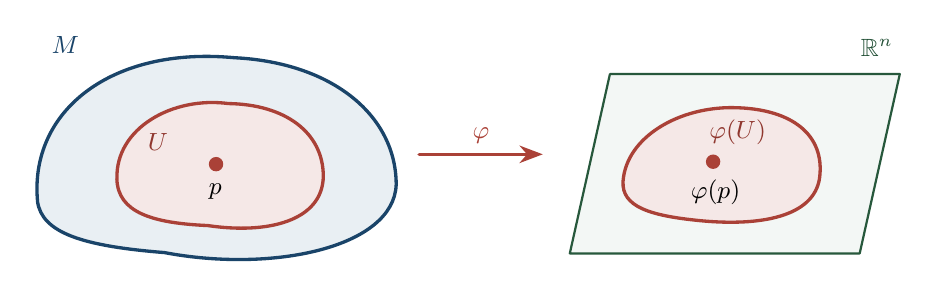
\begin{tikzpicture}[>=Stealth,scale=1.04,line cap=round,line join=round]
% Fragment M oraz wyróżniony otwarty zbiór U.
\filldraw[fill=manifoldblue!10,draw=manifoldblue!75!black,very thick]
 (-5.05,-.55) .. controls (-5.15,.55) and (-4.15,1.34) .. (-2.65,1.2)
 .. controls (-1.43,1.14) and (-.67,.48) .. (-.67,-.35)
 .. controls (-.7,-1.12) and (-2.18,-1.43) .. (-3.5,-1.18)
 .. controls (-4.5,-1.1) and (-5.0,-.94) .. cycle;
\filldraw[fill=manifoldred!12,draw=manifoldred,very thick]
 (-4.08,-.28) .. controls (-4.1,.34) and (-3.4,.73) .. (-2.72,.64)
 .. controls (-2.03,.63) and (-1.56,.29) .. (-1.56,-.25)
 .. controls (-1.57,-.79) and (-2.23,-.96) .. (-2.97,-.85)
 .. controls (-3.65,-.82) and (-4.07,-.69) .. cycle;
\node[manifoldblue!75!black,font=\small\bfseries] at (-4.71,1.35) {$M$};
\node[manifoldred!85!black,font=\small] at (-3.58,.17) {$U$};
\fill[manifoldred] (-2.87,-.1) circle (2.5pt);
\node[font=\small] at (-2.88,-.44) {$p$};
% Obraz mapy w przestrzeni współrzędnych, bez siatki.
\filldraw[fill=manifoldgreen!6,draw=manifoldgreen!70!black,thick]
 (1.45,-1.19)--(4.99,-1.19)--(5.48,1.0)--(1.94,1.0)--cycle;
\filldraw[fill=manifoldred!12,draw=manifoldred,very thick]
 (2.1,-.31) .. controls (2.14,.23) and (2.78,.6) .. (3.45,.59)
 .. controls (4.16,.58) and (4.57,.26) .. (4.5,-.27)
 .. controls (4.43,-.75) and (3.76,-.86) .. (3.04,-.79)
 .. controls (2.43,-.73) and (2.08,-.62) .. cycle;
\node[manifoldgreen!65!black,font=\small\bfseries] at (5.2,1.32) {$\R^n$};
\node[manifoldred!85!black,font=\small] at (3.5,.29) {$\varphi(U)$};
\fill[manifoldred] (3.2,-.07) circle (2.5pt);
\node[font=\small] at (3.23,-.44) {$\varphi(p)$};
\draw[->,very thick,manifoldred] (-.39,.02)--(1.12,.02)
 node[midway,above,font=\small] {$\varphi$};
\end{tikzpicture}
\caption{Mapa $(U,\varphi)$ przenosi otwarty fragment $U\subset M$ na obszar
$\varphi(U)\subset\R^n$; punktowi $p$ przyporządkowuje współrzędne $\varphi(p)$.}
\label{fig:mapa-rozmaitosc}
\end{figure}


\begin{definicja}
Dwie mapy $(U,\varphi)$ i $(V,\psi)$ na $M$ są \emph{zgodne} ($C^\infty$-zgodne), jeżeli
albo $U\cap V=\emptyset$, albo odwzorowania przejścia
\[
\psi\circ\varphi^{-1}\colon\varphi(U\cap V)\to\psi(U\cap V), \qquad
\varphi\circ\psi^{-1}\colon\psi(U\cap V)\to\varphi(U\cap V)
\]
są klasy $C^\infty$ (są to wtedy automatycznie odwzorowania wzajemnie odwrotne między
otwartymi podzbiorami $\R^n$, a więc dyfeomorfizmy).
\end{definicja}



Na Rysunku~\ref{fig:atlas-przejscie-dwie-mapy} pokazano
dwie zgodne mapy i współrzędne punktu
leżącego w ich części wspólnej. Odwzorowanie przejścia
działa \emph{między obrazami tej części wspólnej}, a nie
między całymi $\varphi_\alpha(U_\alpha)$ i
$\varphi_\beta(U_\beta)$, jeśli dziedziny map się różnią.

\begin{figure}[H]
\centering
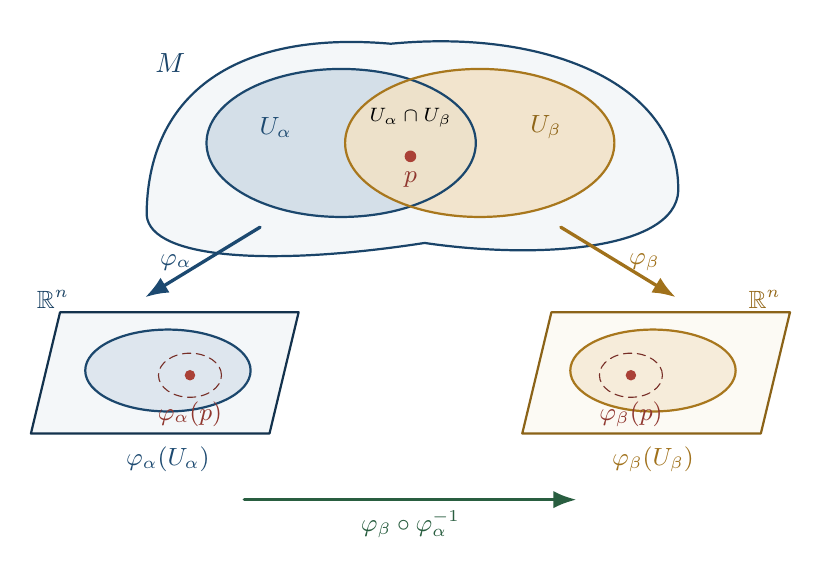
\begin{tikzpicture}[>=Latex,line cap=round,line join=round,
                     font=\small]
  % Fragment rozmaitości i dwa nakładające się obszary map.
  \filldraw[fill=manifoldblue!5,draw=manifoldblue!75!black,thick]
   (-3.35,1.25) .. controls (-3.32,2.76) and (-2.20,3.55)
   .. (-.25,3.38) .. controls (1.72,3.57) and (3.36,2.88)
   .. (3.40,1.59) .. controls (3.48,.77) and (1.68,.63)
   .. (.18,.85) .. controls (-1.90,.53) and (-3.39,.67)
   .. cycle;
  \fill[manifoldblue!22,opacity=.85]
       (-.88,2.12) ellipse (1.71 and .94);
  \fill[manifoldgold!26,opacity=.86]
       (.88,2.12) ellipse (1.71 and .94);
  \draw[manifoldblue!78!black,thick]
       (-.88,2.12) ellipse (1.71 and .94);
  \draw[manifoldgold!82!black,thick]
       (.88,2.12) ellipse (1.71 and .94);
  \node[manifoldblue!75!black,font=\bfseries] at (-3.05,3.13) {$M$};
  \node[manifoldblue!80!black] at (-1.71,2.32) {$U_\alpha$};
  \node[manifoldgold!70!black] at (1.72,2.32) {$U_\beta$};
  \node[font=\scriptsize] at (0,2.44) {$U_\alpha\cap U_\beta$};
  \fill[manifoldred] (0,1.95) circle (2.1pt);
  \node[below,manifoldred!85!black] at (0,1.88) {$p$};
  % Obrazy w dwóch osobnych przestrzeniach współrzędnych.
  \filldraw[fill=manifoldblue!5,draw=manifoldblue!55!black,thick]
       (-4.82,-1.57)--(-1.79,-1.57)--(-1.42,-.03)
       --(-4.45,-.03)--cycle;
  \fill[manifoldblue!15] (-3.08,-.77) ellipse (1.05 and .52);
  \draw[manifoldblue!78!black,thick]
       (-3.08,-.77) ellipse (1.05 and .52);
  \draw[manifoldred!70!black,densely dashed]
       (-2.80,-.83) ellipse (.40 and .28);
  \fill[manifoldred] (-2.80,-.83) circle (1.9pt);
  \node[manifoldred!85!black] at (-2.80,-1.32)
       {$\varphi_\alpha(p)$};
  \node[manifoldblue!70!black] at (-4.54,.13) {$\R^n$};

  \filldraw[fill=manifoldgold!5,draw=manifoldgold!68!black,thick]
       (1.42,-1.57)--(4.45,-1.57)--(4.82,-.03)
       --(1.79,-.03)--cycle;
  \fill[manifoldgold!17] (3.08,-.77) ellipse (1.05 and .52);
  \draw[manifoldgold!82!black,thick]
       (3.08,-.77) ellipse (1.05 and .52);
  \draw[manifoldred!70!black,densely dashed]
       (2.80,-.83) ellipse (.40 and .28);
  \fill[manifoldred] (2.80,-.83) circle (1.9pt);
  \node[manifoldred!85!black] at (2.80,-1.32)
       {$\varphi_\beta(p)$};
  \node[manifoldgold!72!black] at (4.50,.13) {$\R^n$};

  \draw[->,manifoldblue!80!black,very thick]
       (-1.91,1.05)--(-3.37,.16)
       node[midway,left] {$\varphi_\alpha$};
  \draw[->,manifoldgold!78!black,very thick]
       (1.91,1.05)--(3.37,.16)
       node[midway,right] {$\varphi_\beta$};
  \node[manifoldblue!80!black] at (-3.08,-1.90)
       {$\varphi_\alpha(U_\alpha)$};
  \node[manifoldgold!78!black] at (3.08,-1.90)
       {$\varphi_\beta(U_\beta)$};
  \draw[->,manifoldgreen!75!black,very thick]
       (-2.11,-2.41)--(2.11,-2.41)
       node[midway,below] {$\varphi_\beta\circ\varphi_\alpha^{-1}$};
\end{tikzpicture}
\caption{Dwie nakładające się mapy. Przerywane obszary
oznaczają obrazy części wspólnej. Punkt $p$ ma
dwa zapisy współrzędnych, a przejście
$\varphi_\beta\circ\varphi_\alpha^{-1}$ prowadzi
z $\varphi_\alpha(U_\alpha\cap U_\beta)$ do
$\varphi_\beta(U_\alpha\cap U_\beta)$. W atlasie
pozostałe mapy pokrywają ewentualną resztę $M$.}
\label{fig:atlas-przejscie-dwie-mapy}
\end{figure}

\begin{definicja}
\emph{Atlasem} (gładkim, $C^\infty$) na rozmaitości topologicznej $M$ nazywamy rodzinę map
$\mathcal{A}=\{(U_\alpha,\varphi_\alpha)\}_{\alpha\in I}$ taką, że:
\begin{enumerate}[label=(\roman*)]
\item $\bigcup_{\alpha\in I}U_\alpha=M$,
\item mapy $(U_\alpha,\varphi_\alpha)$ oraz $(U_\beta,\varphi_\beta)$ są zgodne dla
wszystkich $\alpha,\beta\in I$.
\end{enumerate}
\end{definicja}



Chcemy teraz porównywać różne atlasy na tej samej przestrzeni topologicznej $M$ — dwa
atlasy powinny wyznaczać tę samą strukturę gładką dokładnie wtedy, gdy razem tworzą
(większy) atlas.

\begin{definicja}
Dwa atlasy $\mathcal{A}_1$, $\mathcal{A}_2$ na $M$ są \emph{równoważne}, $\mathcal A_1\sim
\mathcal A_2$, jeżeli ich suma $\mathcal{A}_1\cup\mathcal{A}_2$ jest atlasem, tzn.\ każda
mapa z $\mathcal{A}_1$ jest zgodna z każdą mapą z $\mathcal{A}_2$.
\end{definicja}

Poniższy lemat techniczny jest kluczowym narzędziem rachunkowym tego paragrafu; wykorzystamy
go dwukrotnie: do dowodu, że $\sim$ jest relacją równoważności, oraz do dowodu istnienia i
jednoznaczności atlasu maksymalnego.

\begin{lemat}\label{lem:zgodnosc-przechodnia}
Niech $(U,\varphi)$, $(W,\eta)$, $(V,\psi)$ będą mapami na $M$ takimi, że $(U,\varphi)$
jest zgodna z $(W,\eta)$, a $(W,\eta)$ jest zgodna z $(V,\psi)$. Wówczas dla dowolnego
punktu $p\in U\cap V\cap W$, odwzorowania $\psi\circ\varphi^{-1}$ i $\varphi\circ\psi^{-1}$
są klasy $C^\infty$ w (odpowiednich) otoczeniach punktów $\varphi(p)$ i $\psi(p)$.
\end{lemat}

\begin{proof}
Na otoczeniu $\varphi(U\cap V\cap W)$ punktu $\varphi(p)$ mamy równość
$\psi\circ\varphi^{-1}=(\psi\circ\eta^{-1})\circ(\eta\circ\varphi^{-1})$; odwzorowanie
$\eta\circ\varphi^{-1}$ jest gładkie na $\varphi(U\cap W)$ (zgodność $(U,\varphi)$ z
$(W,\eta)$), a $\psi\circ\eta^{-1}$ jest gładkie na $\eta(W\cap V)$ (zgodność $(W,\eta)$ z
$(V,\psi)$); złożenie odwzorowań gładkich jest gładkie, więc $\psi\circ\varphi^{-1}$ jest
gładkie w otoczeniu $\varphi(p)$. Analogicznie, na otoczeniu $\psi(p)$:
$\varphi\circ\psi^{-1}=(\varphi\circ\eta^{-1})\circ(\eta\circ\psi^{-1})$ jest złożeniem
odwzorowań gładkich ($\varphi\circ\eta^{-1}$ i $\eta\circ\psi^{-1}$ gładkie, z tych samych
dwóch założeń zgodności), a więc gładkie.
\end{proof}

\begin{stwierdzenie}
Równoważność atlasów jest relacją równoważności na zbiorze wszystkich atlasów na $M$.
\end{stwierdzenie}

\begin{proof}
Zwrotność i symetria są oczywiste z definicji. Sprawdzimy przechodniość. Niech
$\mathcal{A}_1\sim\mathcal{A}_2$ i $\mathcal{A}_2\sim\mathcal{A}_3$; pokażemy, że
$\mathcal{A}_1\sim\mathcal{A}_3$, czyli że dowolna mapa $(U,\varphi)\in\mathcal{A}_1$ jest
zgodna z dowolną mapą $(V,\psi)\in\mathcal{A}_3$. Jeśli $U\cap V=\emptyset$, zgodność jest
trywialna. W przeciwnym razie ustalmy $p\in U\cap V$. Ponieważ $\mathcal{A}_2$ jest atlasem
pokrywającym $M$, istnieje mapa $(W,\eta)\in\mathcal{A}_2$ z $p\in W$. Z założenia
$\mathcal{A}_1\sim\mathcal{A}_2$, mapa $(U,\varphi)$ jest zgodna z $(W,\eta)$; z założenia
$\mathcal{A}_2\sim\mathcal{A}_3$, mapa $(W,\eta)$ jest zgodna z $(V,\psi)$. Na mocy
Lematu~\ref{lem:zgodnosc-przechodnia} (zastosowanego w punkcie $p\in U\cap V\cap W$),
odwzorowania $\psi\circ\varphi^{-1}$ i $\varphi\circ\psi^{-1}$ są gładkie w otoczeniach
odpowiednio $\varphi(p)$ i $\psi(p)$. Ponieważ punkt $p\in U\cap V$ był dowolny, oba te
odwzorowania są gładkie na całych swoich dziedzinach $\varphi(U\cap V)$, $\psi(U\cap V)$
(gładkość jest własnością lokalną). Zatem $(U,\varphi)$ i $(V,\psi)$ są zgodne, co dowodzi
$\mathcal{A}_1\sim\mathcal{A}_3$.
\end{proof}

W praktyce nie chcemy jednak utożsamiać struktury gładkiej z pojedynczym atlasem — dwa
równoważne atlasy powinny wyznaczać \emph{tę samą} strukturę. Wygodnie jest wybrać
kanonicznego reprezentanta każdej klasy równoważności: atlas maksymalny.

\begin{definicja}
Atlas $\mathcal{A}$ na $M$ jest \emph{maksymalny}, jeśli nie jest właściwym podzbiorem
żadnego innego atlasu na $M$, tzn.\ jeśli mapa $(U,\varphi)$ jest zgodna z każdą mapą
należącą do $\mathcal{A}$, to $(U,\varphi)\in\mathcal{A}$.
\end{definicja}

\begin{twierdzenie}\label{tw:atlas-maksymalny}
Każdy atlas $\mathcal{A}$ na $M$ jest zawarty w dokładnie jednym atlasie maksymalnym
$\mathcal{A}^+$, zadanym wzorem
\[
\mathcal{A}^+=\{(U,\varphi)\text{ -- mapa na }M : (U,\varphi)\text{ jest zgodna z każdą
mapą z }\mathcal{A}\}.
\]
Ponadto dwa atlasy $\mathcal{A}_1$, $\mathcal{A}_2$ są równoważne wtedy i tylko wtedy, gdy
$\mathcal{A}_1^+=\mathcal{A}_2^+$.
\end{twierdzenie}

\begin{proof}
\emph{Krok 1: $\mathcal{A}^+$ jest atlasem.} Ponieważ $\mathcal{A}\subseteq\mathcal{A}^+$
(każda mapa z $\mathcal{A}$ jest zgodna z każdą mapą z $\mathcal{A}$, gdyż $\mathcal{A}$
jest atlasem), zbiory dziedzin map z $\mathcal{A}^+$ pokrywają $M$. Pozostaje sprawdzić, że
dowolne dwie mapy $(U,\varphi),(V,\psi)\in\mathcal{A}^+$ są ze sobą zgodne. Ustalmy
$p\in U\cap V$ (dla $U\cap V=\emptyset$ zgodność jest trywialna); ponieważ $\mathcal{A}$
pokrywa $M$, istnieje $(W,\eta)\in\mathcal{A}$ z $p\in W$. Mapa $(U,\varphi)$ jest zgodna z
$(W,\eta)$ (bo $(U,\varphi)\in\mathcal{A}^+$ jest zgodna z każdą mapą z $\mathcal A$), a
$(W,\eta)$ jest zgodna z $(V,\psi)$ (analogicznie, bo $(V,\psi)\in\mathcal A^+$). Na mocy
Lematu~\ref{lem:zgodnosc-przechodnia}, odwzorowania $\psi\circ\varphi^{-1}$,
$\varphi\circ\psi^{-1}$ są gładkie w otoczeniach $\varphi(p)$, $\psi(p)$; wobec dowolności
$p\in U\cap V$, są gładkie na całych dziedzinach $\varphi(U\cap V)$, $\psi(U\cap V)$. Zatem
$\mathcal{A}^+$ jest atlasem.

\emph{Krok 2: $\mathcal{A}^+$ jest maksymalny.} Niech mapa $(U,\varphi)$ będzie zgodna z
każdą mapą należącą do $\mathcal{A}^+$. Ponieważ $\mathcal{A}\subseteq\mathcal{A}^+$, mapa
$(U,\varphi)$ jest w szczególności zgodna z każdą mapą z $\mathcal{A}$, a więc z definicji
$\mathcal{A}^+$ mamy $(U,\varphi)\in\mathcal{A}^+$.

\emph{Krok 3: jednoznaczność.} Niech $\mathcal B\supseteq\mathcal A$ będzie atlasem
maksymalnym. Ponieważ $\mathcal B$ jest atlasem i $\mathcal A\subseteq\mathcal B$, każda
mapa z $\mathcal B$ jest zgodna z każdą mapą z $\mathcal A$ (obie należą do atlasu
$\mathcal B$) — więc $\mathcal B\subseteq\mathcal A^+$ z definicji $\mathcal A^+$.

Odwrotnie, niech $(U,\varphi)\in\mathcal A^+$; pokażemy $(U,\varphi)\in\mathcal B$, co —
wobec dowolności $(U,\varphi)\in\mathcal A^+$ — da $\mathcal A^+\subseteq\mathcal B$, a
wraz z poprzednią inkluzją: $\mathcal B=\mathcal A^+$. Z maksymalności $\mathcal B$
wystarczy pokazać, że $(U,\varphi)$ jest zgodna z każdą mapą $(V,\psi)\in\mathcal B$.
Ustalmy taką mapę i punkt $p\in U\cap V$ (dla $U\cap V=\emptyset$ zgodność jest trywialna).
Ponieważ $\mathcal A$ pokrywa $M$, istnieje $(W,\eta)\in\mathcal A$ z $p\in W$. Mapa
$(U,\varphi)$ jest zgodna z $(W,\eta)$ (bo $(U,\varphi)\in\mathcal A^+$), a $(W,\eta)\in
\mathcal A\subseteq\mathcal B$ jest zgodna z $(V,\psi)\in\mathcal B$ (bo obie należą do
atlasu $\mathcal B$). Na mocy Lematu~\ref{lem:zgodnosc-przechodnia}, $(U,\varphi)$ i
$(V,\psi)$ są zgodne w otoczeniu $p$; wobec dowolności $p\in U\cap V$ — zgodne na całych
dziedzinach. Zatem $(U,\varphi)$ jest zgodna z każdą mapą z $\mathcal B$, więc — z
maksymalności $\mathcal B$ — $(U,\varphi)\in\mathcal B$.

\emph{Krok 4: $\mathcal A_1\sim\mathcal A_2\iff\mathcal A_1^+=\mathcal A_2^+$.}
($\Leftarrow$) Jeśli $\mathcal A_1^+=\mathcal A_2^+=:\mathcal B$, to $\mathcal A_1\subseteq
\mathcal B$ i $\mathcal A_2\subseteq\mathcal B$, a skoro $\mathcal B$ jest atlasem, każda
mapa z $\mathcal A_1$ jest zgodna z każdą mapą z $\mathcal B$, w szczególności z każdą mapą
z $\mathcal A_2$ — czyli $\mathcal A_1\sim\mathcal A_2$.

($\Rightarrow$) Załóżmy $\mathcal A_1\sim\mathcal A_2$. Pokażemy $\mathcal A_1^+\subseteq
\mathcal A_2^+$ (inkluzja odwrotna analogicznie, skąd równość). Niech $(U,\varphi)\in
\mathcal A_1^+$. Ustalmy dowolną mapę $(V,\psi)\in\mathcal A_2$ i (dla $U\cap V\neq
\emptyset$, inaczej trywialnie) punkt $p\in U\cap V$. Ponieważ $\mathcal A_1$ pokrywa $M$,
istnieje $(W,\eta)\in\mathcal A_1$ z $p\in W$. Mapa $(U,\varphi)$ jest zgodna z $(W,\eta)\in
\mathcal A_1$ (bo $(U,\varphi)\in\mathcal A_1^+$), a $(W,\eta)\in\mathcal A_1$ jest zgodna z
$(V,\psi)\in\mathcal A_2$ (bo $\mathcal A_1\sim\mathcal A_2$). Na mocy
Lematu~\ref{lem:zgodnosc-przechodnia}, $(U,\varphi)$ i $(V,\psi)$ są zgodne w otoczeniu
$p$; wobec dowolności $p\in U\cap V$ — na całych dziedzinach. Zatem $(U,\varphi)$ jest
zgodna z $(V,\psi)$; wobec dowolności $(V,\psi)\in\mathcal A_2$, mamy $(U,\varphi)\in
\mathcal A_2^+$.
\end{proof}

Powyższe twierdzenie pozwala oddzielić topologię przestrzeni od
wyboru współrzędnych, w których będziemy różniczkować.

\begin{definicja}[Struktura różniczkowa]\label{def:struktura-rozniczkowa}
\index{struktura rozniczkowa@Struktura różniczkowa}
\emph{Strukturą różniczkową} klasy $C^\infty$ na rozmaitości
topologicznej $M$ nazywamy klasę równoważności atlasów gładkich
na $M$. Równoważnie, na mocy Twierdzenia~\ref{tw:atlas-maksymalny},
jest nią jedyny atlas maksymalny $\mathcal A=\mathcal A_0^+$
zawierający dowolny atlas $\mathcal A_0$ z tej klasy. Mapy
należące do $\mathcal A$ nazywamy \emph{dopuszczalnymi}.
\end{definicja}

\begin{definicja}[Rozmaitość gładka]\label{def:rozmaitosc-gladka}
\index{rozmaitosc gladka@Rozmaitość gładka}
\emph{Rozmaitością gładką} (klasy $C^\infty$) wymiaru $n$
nazywamy parę $(M,\mathcal A)$, gdzie $M$ jest rozmaitością
topologiczną wymiaru $n$, a $\mathcal A$ jest strukturą
różniczkową zapisaną jako atlas maksymalny.
\end{definicja}

W praktyce wystarczy podać mały atlas $\mathcal A_0$:
wyznacza on jednoznacznie strukturę $\mathcal A_0^+$.
Topologia określa, które mapy współrzędnych są homeomorfizmami;
struktura różniczkowa określa dodatkowo, które przejścia
między nimi są gładkie.

\begin{przyklad}[Różne struktury na tej samej przestrzeni]
Na topologicznej prostej $\R$ atlas $\mathcal A_{\mathrm{std}}$
z mapą $\id\colon\R\to\R$ i atlas $\mathcal A_h$ z mapą
$h\colon\R\to\R$, $h(x)=x^3$, są osobno atlasami gładkimi.
Nie są równoważne: w jednym kierunku
przejście jest dane przez $h^{-1}(u)=\sqrt[3]{u}$,
które nie jest różniczkowalne w zerze.
Definiują zatem różne struktury na \emph{ustalonym} zbiorze
topologicznym $\R$, choć otrzymane rozmaitości są
dyfeomorficzne (w sensie definicji~\ref{def dyfeo}): dyfeomorfizm
$h\colon(\R,\mathcal A_h^+)\to(\R,\mathcal A_{\mathrm{std}}^+)$
ma w odpowiednich mapach współrzędnych postać identyczności.
\end{przyklad}

\begin{uwaga}[Intuicja: mapa, atlas i rozmaitość]
Najprostszym sposobem zrozumienia pojęć \emph{mapy}, \emph{atlasu} i
\emph{rozmaitości} jest analogia z powierzchnią Ziemi.

Powierzchnia Ziemi jest obiektem zakrzywionym i nie możemy przedstawić jej
w całości na jednej płaskiej kartce bez zniekształceń. Możemy jednak wybrać
niewielki fragment powierzchni, na przykład okolice Krakowa, i przedstawić go
na płaskiej mapie. Matematycznie dokładnie taką rolę pełni \emph{mapa}
rozmaitości.

Jeżeli $M$ jest rozmaitością, to mapa jest parą $(U,\varphi)$, gdzie
$U\subset M$ jest otwartym fragmentem rozmaitości, a $\varphi\colon U\longrightarrow \varphi(U)\subset\mathbb{R}^n$
jest homeomorfizmem. Oznacza to, że punkty znajdujące się w $U$ możemy opisać
za pomocą zwykłych współrzędnych $(x^1,\ldots,x^n)\in\mathbb{R}^n$.
Można więc myśleć o $\varphi$ jako o sposobie ``rozłożenia'' niewielkiego
fragmentu rozmaitości na płaskiej przestrzeni $\mathbb{R}^n$.

Jedna mapa zazwyczaj nie wystarcza do opisania całej przestrzeni. Podobnie
jedna mapa geograficzna przedstawiająca okolice Krakowa nie opisuje całej
powierzchni Ziemi. Potrzebujemy wielu map $(U_\alpha,\varphi_\alpha)$,
których dziedziny pokrywają całą przestrzeń:
\[
    M=\bigcup_{\alpha}U_\alpha.
\]
Taki zbiór map nazywamy \emph{atlasem}.

Jeżeli dwa obszary $U_\alpha$ i $U_\beta$ nachodzą na siebie, to ten sam punkt
rozmaitości może mieć dwa różne opisy współrzędnościowe. Przejście pomiędzy
nimi opisuje odwzorowanie $\varphi_\beta\circ\varphi_\alpha^{-1}$,
zwane odwzorowaniem przejścia. Można je porównać do przeliczania współrzędnych
tego samego miejsca pomiędzy dwiema zachodzącymi na siebie mapami
geograficznymi.

\emph{Rozmaitość} jest zatem przestrzenią, która globalnie może być
skomplikowana lub zakrzywiona, ale w dostatecznie małym otoczeniu każdego
punktu wygląda jak zwykła przestrzeń euklidesowa $\mathbb{R}^n$.

W skrócie:
\[
\boxed{
\begin{array}{ccl}
\text{mapa}      &\longleftrightarrow& \text{lokalny układ współrzędnych},\\[2mm]
\text{atlas}     &\longleftrightarrow& \text{zbiór map opisujących całą przestrzeń},\\[2mm]
\text{rozmaitość}&\longleftrightarrow& \text{przestrzeń lokalnie wyglądająca jak }\mathbb{R}^n.
\end{array}}
\]

Przykładowo sfera $S^2$ nie jest płaską częścią $\mathbb{R}^2$, ale każdy jej
dostatecznie mały fragment można opisać za pomocą dwóch współrzędnych.
Dlatego $S^2$ jest dwuwymiarową rozmaitością.
\end{uwaga}

Od tej pory, mówiąc o rozmaitości $M$, będziemy mieli na myśli rozmaitość gładką — parę
$(M,\mathcal{A})$ — pomijając $\mathcal{A}$ w oznaczeniach, gdy nie prowadzi to do
nieporozumień.

\section{Rozmaitości z brzegiem}
\label{sec:rozmaitosci-z-brzegiem-1}
\index{brzeg rozmaitosci@Brzeg rozmaitości}

Wnętrze dysku wygląda lokalnie jak otwarty zbiór w $\R^n$,
ale punkt na jego brzegu ma tylko jedną stronę. Modelem takiego
otoczenia jest półprzestrzeń $\mathbb H^n=\{(x^1,\ldots,x^n)\in\R^n:x^n\geq0\}, \ n\geq1$.
Otwartość podzbioru $\mathbb H^n$ rozumiemy w topologii względnej.

\begin{definicja}[Rozmaitość gładka z brzegiem]
\index{rozmaitosc gladka z brzegiem@Rozmaitość gładka z brzegiem}
\label{def:rozmaitosc-z-brzegiem-1}
\emph{Rozmaitość gładka z brzegiem} wymiaru $n\geq1$ to przestrzeń
Hausdorffa spełniająca drugi aksjomat przeliczalności, wyposażona
w atlas homeomorfizmów
$\varphi_\alpha:U_\alpha\to V_\alpha$ na zbiory
$V_\alpha$ otwarte w $\mathbb H^n$. Na częściach wspólnych
odwzorowania przejścia i ich odwrotności mają być gładkie:
w otoczeniu każdego punktu rozumie się przez to istnienie
gładkiego przedłużenia na otwarty zbiór w $\R^n$.
Maksymalny atlas zgodny z tym atlasem wyznacza strukturę gładką,
tak jak w Twierdzeniu~\ref{tw:atlas-maksymalny}.
\emph{Brzegiem rozmaitości} nazywamy zbiór
\[
 \partial M=\{p\in M:\varphi_\alpha(p)^n=0
             \text{ w pewnej mapie }(U_\alpha,\varphi_\alpha)\}.
\]
Pozostałe punkty tworzą wnętrze $M^\circ=M\setminus\partial M$.
Dla wymiaru $0$ przyjmujemy $\partial M=\varnothing$.
\end{definicja}

Warunek „w pewnej mapie” jest poprawny dzięki następującemu
faktowi; jednocześnie pokazuje, że brzeg nie zależy od wyboru
współrzędnych.

\begin{stwierdzenie}[Niezależność brzegu od mapy]
\label{prop:brzeg-niezalezny-1}
Dla $n\geq1$, jeśli $p$ ma ostatnią współrzędną równą $0$ w jednej
mapie półprzestrzennej, to ma ją równą $0$ w każdej
mapie półprzestrzennej, której dziedzina zawiera $p$.
Zbiór $\partial M$ jest zamknięty w $M$ i z map ograniczonych
do $\partial M$ otrzymuje strukturę gładkiej
rozmaitości wymiaru $n-1$ bez brzegu.
\end{stwierdzenie}
\begin{proof}
Przypuśćmy, że $\varphi(p)$ leży na płaszczyźnie
$x^n=0$, a $\psi(p)$ jest punktem wnętrza $\mathbb H^n$.
Ograniczmy mapy do wspólnego dostatecznie małego otoczenia
$p$. Wtedy $\psi$ odwzorowuje je na zbiór otwarty w $\R^n$,
a $\varphi\circ\psi^{-1}$ jest ciągłą injekcją tego zbioru
do $\R^n$. Twierdzenie Brouwera o niezmienniczości obszaru
orzeka, że obraz takiej injekcji jest otwarty w $\R^n$.
Obraz leży jednak w $\mathbb H^n$ i zawiera punkt
$\varphi(p)$ na jego płaszczyźnie brzegowej, więc nie może
być otwarty w $\R^n$. Sprzeczność dowodzi pierwszej tezy.
Dokładne sformułowanie użytego wyniku zewnętrznego podaje
\href{https://pi.math.cornell.edu/~hatcher/AT/AT.pdf}
{A. Hatcher, \emph{Algebraic Topology}, twierdzenie 2B.3}.

W każdej mapie punkty z $x^n>0$ tworzą zbiór otwarty.
Zatem $M^\circ$ jest otwarty, a $\partial M$ zamknięty.
Ograniczenie mapy $\varphi$ do
$U\cap\partial M$ przyjmuje wartości w otwartym
podzbiorze $\R^{n-1}\times\{0\}$. Przejścia między
tymi ograniczeniami są gładkie, bo są ograniczeniami
gładkich przedłużeń przejść na $\R^n$; to samo dotyczy
odwrotności. Są to więc mapy gładkiej rozmaitości
wymiaru $n-1$. Każda z nich ma obraz otwarty w całej
$\R^{n-1}$, czyli $\partial M$ nie ma własnego brzegu.
\end{proof}

W punkcie brzegu definiujemy $T_pM$ przez
wektory współrzędnych w półprzestrzennej mapie,
równoważnie przez derywacje gładkich kiełków
funkcji w $p$. Pełną konstrukcję i niezależność od przedłużeń
podamy po wprowadzeniu przestrzeni stycznej, w
Stwierdzeniu~\ref{prop:styczna-brzeg-1}. Ten model ma $n$ niezależnych
kierunków: $T_pM\cong\R^n$, natomiast
$T_p\partial M\cong\{v\in\R^n:v^n=0\}$ ma wymiar $n-1$.
Wektor o ujemnej ostatniej współrzędnej należy do $T_pM$,
choć nie jest prędkością krzywej biegnącej od $p$ do wnętrza
przy dodatnim czasie. Przykładowo $T_0[0,1]\cong\R$,
podczas gdy $T_0\partial[0,1]=0$.
Model przez krzywe określone na otwartym przedziale,
omówiony w Sekcji~\ref{sec:przestrzen-styczna},
dotyczy punktów wnętrza: w punkcie brzegu
dwustronna krzywa w $M$ nie reprezentuje
kierunku poprzecznego do brzegu.

\begin{przyklad}[Kula, okrąg i brzeg otaczającej przestrzeni]
\label{prz:brzeg-kula-okrag-1}
Domknięta kula $D^n=\{x\in\R^n:|x|\leq1\}$ ma brzeg
rozmaitościowy $S^{n-1}$. Rzeczywiście, przy $|p|=1$
funkcja $\rho(x)=1-|x|^2$ ma niezerową różniczkę
$\dd\rho_p(v)=-2\langle p,v\rangle$. Twierdzenie o funkcji
odwrotnej pozwala użyć $\rho$ jako ostatniej lokalnej
współrzędnej, zatem $D^n$ odpowiada warunkowi $\rho\geq0$.
Z kolei brzeg okręgu $S^1\subset\R^2$ jako rozmaitości
(w sensie Definicji~\ref{def:rozmaitosc-z-brzegiem-1})
jest pusty: $\partial S^1=\varnothing$. Jego brzeg topologiczny
jako \emph{podzbioru $\R^2$} jest natomiast całym $S^1$: okrąg ma
puste wnętrze w $\R^2$ i jest domknięty.
Te dwa znaczenia słowa „brzeg” trzeba odróżniać.
\end{przyklad}

Produkt dwóch rozmaitości z brzegiem może mieć
\emph{naroża}. W kwadracie $[0,1]^2$ przy wierzchołku
naturalny model pochodzący z zanurzenia to
$[0,\infty)^2$, z dwiema ścianami brzegowymi.
W rachunku uchwytów spotkamy taki model na
$\partial D^k\times\partial D^{n-k}$; naroże można
zaokrąglić w małym otoczeniu, zachowując części
odległe od niego. To operacja na gładkiej geometrii
brzegu, a nie zmiana tego, które punkty są brzegowe
topologicznie. Kołnierze i takie zaokrąglanie pojawią się
w Sekcji~\ref{sec:kolnierz-15} i przy uchwytach w
Sekcji~\ref{sec:uchwyt-morse-17}.

\section{Rozmaitości zespolone}

Analogicznie do konstrukcji z poprzedniego paragrafu, możemy modelować rozmaitość lokalnie
nie na $\R^n$, lecz na $\C^n$, żądając przy tym, by odwzorowania przejścia między mapami
były holomorficzne, a nie tylko gładkie.

\begin{definicja}
\emph{Rozmaitością zespoloną} wymiaru (zespolonego) $n$ nazywamy przestrzeń Hausdorffa $M$
spełniającą drugi aksjomat przeliczalności, wyposażoną w atlas $\{(U_\alpha,\varphi_\alpha)\}$
map $\varphi_\alpha\colon U_\alpha\to\varphi_\alpha(U_\alpha)\subseteq\C^n$ (homeomorfizmów
na zbiory otwarte w $\C^n\cong\R^{2n}$), takich że odwzorowania przejścia
\[
\varphi_\beta\circ\varphi_\alpha^{-1}\colon\varphi_\alpha(U_\alpha\cap U_\beta)\to
\varphi_\beta(U_\alpha\cap U_\beta)
\]
są \emph{holomorficzne} (jako odwzorowania między otwartymi podzbiorami $\C^n$), wraz z
maksymalnym takim atlasem (konstrukcja atlasu maksymalnego przebiega dosłownie tak samo,
jak w Sekcji~\ref{sec:atlas}, z ,,gładki'' zastąpionym przez ,,holomorficzny'' — złożenie odwzorowań
holomorficznych jest holomorficzne, więc Lemat~\ref{lem:zgodnosc-przechodnia} i
Twierdzenie~\ref{tw:atlas-maksymalny} przenoszą się bez zmian).
\end{definicja}

\begin{uwaga}
Utożsamiając $\C^n\cong\R^{2n}$ (przez część rzeczywistą i urojoną każdej współrzędnej)
oraz przypominając, że każde odwzorowanie holomorficzne jest w szczególności odwzorowaniem
gładkim (klasy $C^\infty$) w sensie rzeczywistym (ze wzoru całkowego
Cauchy'ego na małym polidysku wynika lokalne rozwinięcie w szereg potęgowy,
który można różniczkować wyraz po wyrazie), widzimy, że \emph{każda rozmaitość zespolona
wymiaru $n$ jest w naturalny sposób rzeczywistą rozmaitością gładką wymiaru $2n$}. Implikacja
odwrotna jest fałszywa: nie każda parzystowymiarowa rozmaitość gładka dopuszcza strukturę
zespoloną (a nawet jeśli dopuszcza, struktura taka zwykle nie jest jednoznaczna).
\end{uwaga}

\begin{przyklad}[Zespolona przestrzeń rzutowa]
Niech $\C_*:=\C\setminus\{0\}$ oznacza zbiór niezerowych
liczb zespolonych.
Zespolonym odpowiednikiem $\mathbb{RP}^n$ z
Przykładu~\ref{prz:RPn} jest przestrzeń ilorazowa $\mathbb{CP}^n := (\C^{n+1}\setminus\{0\})/\!\sim$,
gdzie
\[
z\sim w
\iff
\exists\,\lambda\in\C_*
\quad\text{takie, że}\quad
z=\lambda w.
\]
Przestrzeń $\mathbb{CP}^n$ wyposażamy w topologię ilorazową.
Punkty zapisujemy w postaci $[z^0:z^1:\dots:z^n]$,
przy czym
\[
[z^0:\dots:z^n]
=
[\lambda z^0:\dots:\lambda z^n]
\qquad
\text{dla każdego }\lambda\in\C_*.
\]

Dla $i=0,\dots,n$ definiujemy $U_i = \{[z^0:\dots:z^n]\in\mathbb{CP}^n:z^i\neq0\}$.
Zbiory $U_i$ są otwarte i pokrywają całą przestrzeń $\mathbb{CP}^n$.
Na każdym z nich definiujemy mapę $\varphi_i:U_i\longrightarrow\C^n$
wzorem
\[
\varphi_i([z^0:\dots:z^n])
=
\left(
\frac{z^0}{z^i},
\dots,
\frac{z^{i-1}}{z^i},
\frac{z^{i+1}}{z^i},
\dots,
\frac{z^n}{z^i}
\right).
\]
Jej odwrotność jest dana jawnie przez
\[
\varphi_i^{-1}
(w^0,\dots,w^{i-1},w^{i+1},\dots,w^n)
=
[w^0:\dots:w^{i-1}:1:w^{i+1}:\dots:w^n].
\]
Sprawdźmy także ciągłość, której nie daje sama bijektywność.
Niech $\pi\colon\C^{n+1}\setminus\{0\}\to\mathbb{CP}^n$ będzie
rzutowaniem ilorazowym. Przeciwobraz $\pi^{-1}(U_i)=\{z:z^i\ne0\}$
jest otwarty, zatem $U_i$ jest otwarty. Ograniczenie
$\pi\colon\pi^{-1}(U_i)\to U_i$ także jest odwzorowaniem ilorazowym:
otwarty w $\pi^{-1}(U_i)$ przeciwobraz podzbioru $U_i$ jest otwarty
w całej dziedzinie $\pi$, więc sam podzbiór jest otwarty w ilorazie.
Składowe $\varphi_i\circ\pi$ są ciągłymi ilorazami współrzędnych;
z własności topologii ilorazowej wynika ciągłość $\varphi_i$.
Podany wzór na $\varphi_i^{-1}$ jest złożeniem ciągłego wstawienia
współrzędnej $1$ z $\pi$. Każda $\varphi_i$ jest więc homeomorfizmem
pomiędzy $U_i$ a $\C^n$.

Na przecięciu $U_i\cap U_j$ ten sam punkt przestrzeni
$\mathbb{CP}^n$ posiada dwa różne opisy współrzędnościowe.
Przejście pomiędzy nimi jest opisane przez odwzorowanie $\varphi_j\circ\varphi_i^{-1}$.
Jego składowe są ilorazami wielomianów zespolonych, przy czym
mianowniki nie znikają na dziedzinie odwzorowania. Odwzorowania
przejścia są zatem holomorficzne. Aksjomat Hausdorffa i istnienie
przeliczalnej bazy topologii sprawdzimy w dowodzie
twierdzenia~\ref{thm:rzutowe-zwarte-1}. Łącznie daje to strukturę
rozmaitości zespolonej wymiaru $n$ na $\mathbb{CP}^n$, a więc również
rzeczywistej rozmaitości gładkiej wymiaru $2n$.

Rozważmy teraz szczególny przypadek $n=1$. Otrzymujemy
\emph{sferę Riemanna} $\mathbb{CP}^1$.
Mamy wówczas dwa zbiory $U_0=\{[z^0:z^1]:z^0\neq0\}, \ U_1=\{[z^0:z^1]:z^1\neq0\}$,
oraz mapy
\[
\varphi_0:U_0\longrightarrow\C,
\qquad
\varphi_0([z^0:z^1])=\frac{z^1}{z^0},
\]
i
\[
\varphi_1:U_1\longrightarrow\C,
\qquad
\varphi_1([z^0:z^1])=\frac{z^0}{z^1}.
\]
Każda z tych map identyfikuje odpowiedni fragment
$\mathbb{CP}^1$ z kopią płaszczyzny zespolonej $\C$.

Na przecięciu $U_0\cap U_1 = \{[z^0:z^1]:z^0\neq0,\ z^1\neq0\}$
ten sam punkt ma w pierwszej mapie współrzędną $w = \varphi_0([z^0:z^1]) = \frac{z^1}{z^0}$,
natomiast w drugiej mapie współrzędną $v = \varphi_1([z^0:z^1]) = \frac{z^0}{z^1}$.
Stąd $v=\frac1w$.
Odwzorowanie przejścia ma więc postać $\varphi_1\circ\varphi_0^{-1}(w) = \frac1w, \ w\in\C_*$.

Możemy zatem patrzeć na $\mathbb{CP}^1$ jako na przestrzeń otrzymaną
z dwóch rozłącznych kopii płaszczyzny zespolonej, $\C_0\sqcup\C_1$,
przez utożsamienie punktów należących do ich niezerowych części zgodnie
z regułą $w\in\C_0\setminus\{0\} \quad\sim\quad \frac1w\in\C_1\setminus\{0\}$.
W tym właśnie sensie mówi się, że dwie kopie $\C$ są
\emph{sklejone za pomocą odwzorowania przejścia} $w\longmapsto\frac1w$.
Nie sklejamy więc całych płaszczyzn punkt po punkcie, lecz utożsamiamy
jedynie te punkty obu kopii $\C$, które odpowiadają temu samemu punktowi
przestrzeni $\mathbb{CP}^1$ na części wspólnej $U_0\cap U_1$.

Punkt $0\in\C_0$ odpowiada punktowi $[1:0]\in\mathbb{CP}^1$,
natomiast punkt $0\in\C_1$ odpowiada punktowi $[0:1]\in\mathbb{CP}^1$.
W szczególności, patrząc wyłącznie przez mapę $\varphi_0$, punkt
$[0:1]$ można interpretować jako dodatkowy punkt w nieskończoności.
Dlatego często zapisuje się $\mathbb{CP}^1 \cong \C\cup\{\infty\}$.

Przestrzeń $\mathbb{CP}^1$ jest dyfeomorficzna ze sferą $S^2$.
Trzeba jednak uważać na wybór zespolonych współrzędnych
stereograficznych. Zwykłe rzeczywiste rzuty stereograficzne z
Przykładu~\ref{prz:sfera}, po utożsamieniu $\R^2=\C$, prowadzą do
odwzorowania przejścia $w\longmapsto\frac{w}{|w|^2} = \frac1{\overline{w}}$,
które nie jest holomorficzne.

Aby otrzymać strukturę zespoloną zgodną ze strukturą na
$\mathbb{CP}^1$, wybieramy na $S^2$ współrzędne
\[
\zeta_N(x)
=
\frac{x^1+ix^2}{1-x^3},
\qquad
\zeta_S(x)
=
\frac{x^1-ix^2}{1+x^3}.
\]
Wtedy na części wspólnej zachodzi $\zeta_S\circ\zeta_N^{-1}(w) = \frac1w$.

Jawny dyfeomorfizm $H:\mathbb{CP}^1\longrightarrow S^2$
jest dany wzorem
\[
H([z^0:z^1])
=
\frac{
\big(
2\Re(\overline{z^0}z^1),
2\Im(\overline{z^0}z^1),
|z^1|^2-|z^0|^2
\big)
}{
|z^0|^2+|z^1|^2
}.
\]
Skalowanie obu współrzędnych przez $\lambda\neq0$ mnoży licznik
i mianownik przez $|\lambda|^2$, dlatego wzór jest dobrze określony
na klasach równoważności.

Ponadto
\[
4|z^0|^2|z^1|^2
+
\big(|z^1|^2-|z^0|^2\big)^2
=
\big(|z^0|^2+|z^1|^2\big)^2,
\]
co pokazuje, że obraz odwzorowania $H$ leży na sferze $S^2$.

W wybranych współrzędnych mamy $\zeta_N\circ H=\varphi_0, \ \zeta_S\circ H=\varphi_1$.
Pierwsza z tych równości daje bijekcję $U_0\longrightarrow S^2\setminus\{N\}$,
natomiast pozostały punkt $[0:1]$
przechodzi na biegun północny $N$.
W lokalnych współrzędnych odwzorowanie $H$ oraz jego odwrotność są
tożsamościami, co pokazuje, że $\mathbb{CP}^1\cong S^2$
jako rozmaitości gładkie.
\end{przyklad}


\begin{figure}[h]
\centering
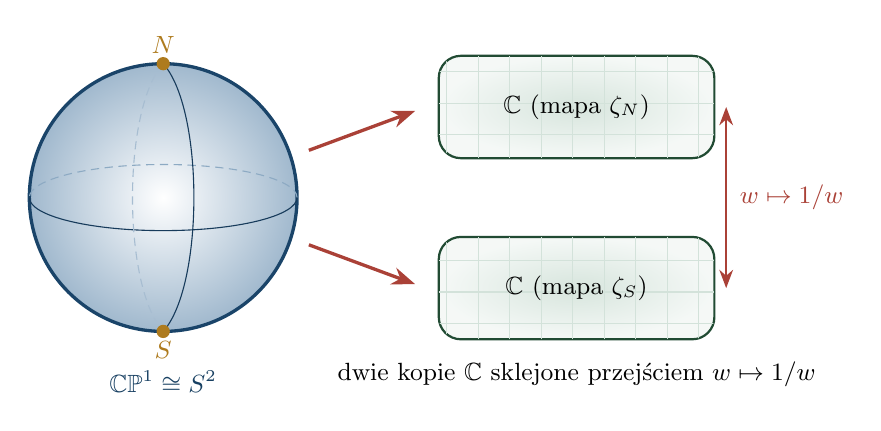
\begin{tikzpicture}[>=Stealth,scale=1]
% Sfera: jasna plama i podział równika na część widoczną oraz ukrytą.
\shade[inner color=white,outer color=manifoldblue!43] (0,0) circle (1.7);
\draw[manifoldblue!75!black,very thick] (0,0) circle (1.7);
\draw[manifoldblue!52,densely dashed,thin]
  (1.7,0) arc[start angle=0,end angle=180,x radius=1.7,y radius=.42];
\draw[manifoldblue!65!black,thin]
  (-1.7,0) arc[start angle=180,end angle=360,x radius=1.7,y radius=.42];
\draw[manifoldblue!40,densely dashed,thin] (0,1.7)
  .. controls (-.52,1.12) and (-.52,-1.12) .. (0,-1.7);
\draw[manifoldblue!65!black,thin] (0,1.7)
  .. controls (.52,1.12) and (.52,-1.12) .. (0,-1.7);
% bieguny
\fill[manifoldgold!85!black] (0,1.7) circle (2.4pt) node[above,font=\small]{$N$};
\fill[manifoldgold!85!black] (0,-1.7) circle (2.4pt) node[below,font=\small]{$S$};
\node[manifoldblue!70!black,font=\small] at (0,-2.35) {$\mathbb{CP}^1\cong S^2$};
% --- strzałki do płaszczyzn C ---
\draw[->,very thick,manifoldred] (1.85,0.6) -- (3.2,1.1);
\draw[->,very thick,manifoldred] (1.85,-0.6) -- (3.2,-1.1);
% --- dwie kopie C (zaokrąglone) ---
% górna
\shade[inner color=manifoldgreen!20, outer color=manifoldgreen!5, rounded corners=8pt]
  (3.5,0.5) rectangle (7.0,1.8);
\draw[manifoldgreen!60!black,thick,rounded corners=8pt]
  (3.5,0.5) rectangle (7.0,1.8);
\begin{scope}
  \clip[rounded corners=8pt] (3.5,0.5) rectangle (7.0,1.8);
  \draw[step=0.4,manifoldgreen!22,thin] (3.5,0.5) grid (7.0,1.8);
\end{scope}
\node[font=\small] at (5.25,1.15) {$\C$ (mapa $\zeta_N$)};
% dolna
\shade[inner color=manifoldgreen!20, outer color=manifoldgreen!5, rounded corners=8pt]
  (3.5,-1.8) rectangle (7.0,-0.5);
\draw[manifoldgreen!60!black,thick,rounded corners=8pt]
  (3.5,-1.8) rectangle (7.0,-0.5);
\begin{scope}
  \clip[rounded corners=8pt] (3.5,-1.8) rectangle (7.0,-0.5);
  \draw[step=0.4,manifoldgreen!22,thin] (3.5,-1.8) grid (7.0,-0.5);
\end{scope}
\node[font=\small] at (5.25,-1.15) {$\C$ (mapa $\zeta_S$)};
% przejście w↦1/w
\draw[<->,thick,manifoldred] (7.15,1.15) -- (7.15,-1.15);
\node[manifoldred,font=\small,right] at (7.2,0) {$w\mapsto 1/w$};
\node[font=\small] at (5.25,-2.25) {dwie kopie $\C$ sklejone przejściem $w\mapsto 1/w$};
\end{tikzpicture}
\caption{Schematyczna interpretacja $\mathbb{CP}^1$ jako sfery Riemanna:
dwie mapy zespolone pokrywają sferę; w mapie południowej odwrócono
znak drugiej współrzędnej rzeczywistej. Przejście $1/w$ jest określone dla $w\ne0$.}
\label{fig:cp1}
\end{figure}

\section{Odwzorowania gładkie między rozmaitościami}

\begin{definicja}
Niech $M$, $N$ będą rozmaitościami gładkimi wymiarów odpowiednio $m$, $n$. Odwzorowanie
$F\colon M\to N$ jest \emph{gładkie} (klasy $C^\infty$) w punkcie $p\in M$, jeżeli dla
pewnej (równoważnie: każdej) mapy dopuszczalnej $(U,\varphi)$ wokół $p$ i mapy
dopuszczalnej $(V,\psi)$ wokół $F(p)$ z $F(U)\subseteq V$, odwzorowanie
$\psi\circ F\circ\varphi^{-1}\colon\varphi(U)\to\psi(V)$
jest gładkie (klasy $C^\infty$) w pewnym otwartym otoczeniu
$\varphi(p)$. Odwzorowanie $F$ jest gładkie, jeśli jest gładkie w każdym punkcie $p\in M$.
Zbiór wszystkich gładkich funkcji $M\to\R$ oznaczamy $C^\infty(M)$.
\end{definicja}
\begin{figure}[ht]
\centering
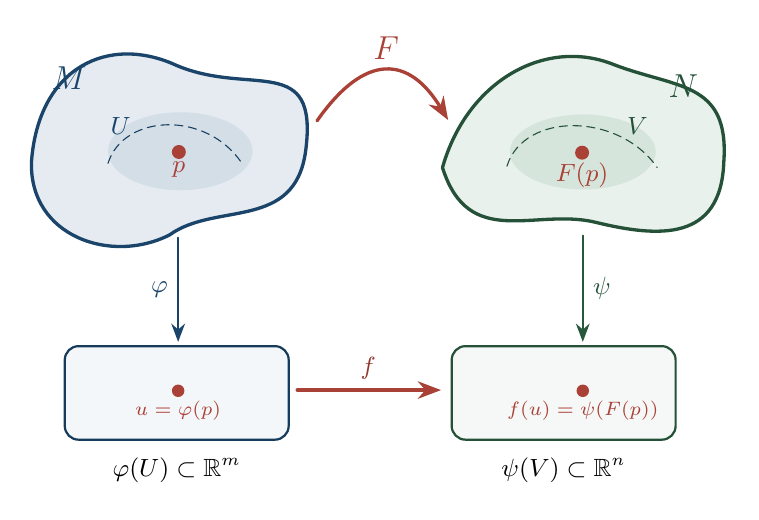
\begin{tikzpicture}[>=Stealth,scale=.9,line cap=round,line join=round]
% Dwie pofalowane powierzchnie z siatką lokalnych współrzędnych.
\def\Mshape{(-4.75,.2) .. controls (-4.65,1.55) and (-3.65,2.0) .. (-2.7,1.56)
 .. controls (-1.65,1.12) and (-.7,1.75) .. (-.88,.36)
 .. controls (-1.03,-.78) and (-2.15,-.36) .. (-2.8,-.83)
 .. controls (-3.63,-1.25) and (-4.78,-.85) .. cycle}
\def\Nshape{(1.05,.12) .. controls (1.4,1.35) and (2.5,1.95) .. (3.45,1.58)
 .. controls (4.35,1.23) and (5.1,1.35) .. (5.02,.2)
 .. controls (4.98,-.93) and (4.1,-.87) .. (3.2,-.65)
 .. controls (2.35,-.45) and (1.42,-1.05) .. cycle}
\fill[manifoldblue!12] \Mshape;
\begin{scope}
\clip \Mshape;
\fill[manifoldblue!24,opacity=.65] (-2.65,.35) ellipse (1.02 and .55);
\end{scope}
\draw[manifoldblue!75!black,very thick] \Mshape;
\draw[manifoldblue!70!black,densely dashed] (-3.67,.18) .. controls (-3.45,.88) and (-2.28,.93) .. (-1.78,.18);
\fill[manifoldgreen!11] \Nshape;
\begin{scope}
\clip \Nshape;
\fill[manifoldgreen!25,opacity=.65] (3.03,.34) ellipse (1.03 and .53);
\end{scope}
\draw[manifoldgreen!65!black,very thick] \Nshape;
\draw[manifoldgreen!65!black,densely dashed] (1.96,.14) .. controls (2.2,.91) and (3.54,.9) .. (4.08,.12);
\node[font=\large\bfseries,manifoldblue!75!black] at (-4.22,1.38) {$M$};
\node[font=\large\bfseries,manifoldgreen!65!black] at (4.45,1.27) {$N$};
\node[font=\small,manifoldblue!75!black] at (-3.49,.7) {$U$};
\node[font=\small,manifoldgreen!65!black] at (3.8,.7) {$V$};
\fill[manifoldred] (-2.67,.34) circle (2.8pt) node[below,font=\small] {$p$};
\fill[manifoldred] (3.02,.33) circle (2.8pt) node[below,font=\small] {$F(p)$};
\draw[->,very thick,manifoldred] (-.72,.78) .. controls (-.04,1.75) and (.58,1.7) .. (1.13,.79)
  node[midway,above,font=\large\bfseries] {$F$};
% Dwie euklidesowe mapy z zaznaczonymi odpowiadającymi sobie punktami.
\fill[manifoldblue!5,rounded corners=5pt] (-4.28,-3.72) rectangle (-1.12,-2.4);
\draw[manifoldblue!65!black,thick,rounded corners=5pt] (-4.28,-3.72) rectangle (-1.12,-2.4);
\fill[manifoldgreen!5,rounded corners=5pt] (1.18,-3.72) rectangle (4.34,-2.4);
\draw[manifoldgreen!65!black,thick,rounded corners=5pt] (1.18,-3.72) rectangle (4.34,-2.4);
\draw[->,thick,manifoldblue!75!black] (-2.68,-.87)--(-2.68,-2.34)
  node[midway,left,font=\small] {$\varphi$};
\draw[->,thick,manifoldgreen!70!black] (3.03,-.84)--(3.03,-2.34)
  node[midway,right,font=\small] {$\psi$};
\fill[manifoldred] (-2.68,-3.03) circle (2.5pt) node[below,font=\scriptsize] {$u=\varphi(p)$};
\fill[manifoldred] (3.03,-3.03) circle (2.5pt) node[below,font=\scriptsize] {$f(u)=\psi(F(p))$};
\draw[->,very thick,manifoldred] (-1.0,-3.02)--(1.03,-3.02);
\node[font=\small\bfseries,manifoldred!85!black] at (0,-2.71) {$f$};
\node[font=\small] at (-2.7,-4.15) {$\varphi(U)\subset\R^m$};
\node[font=\small] at (2.76,-4.15) {$\psi(V)\subset\R^n$};
\end{tikzpicture}
\caption{Odwzorowanie $F\colon M\to N$ oraz jego lokalny zapis współrzędnościowy. Po wybraniu map $(U,\varphi)$ i $(V,\psi)$ gładkość $F$ bada się poprzez zwykłe odwzorowanie $\psi\circ F\circ\varphi^{-1}$ między otwartymi podzbiorami przestrzeni euklidesowych.}
\label{fig:odwzorowanie-gładkie}
\end{figure}

\begin{uwaga}
Definicja gładkości nie zależy od wyboru map. Niech $(U,\varphi)$ oraz
$(V,\psi)$ będą mapami wokół odpowiednio $p$ i $F(p)$, dla których
odwzorowanie $\psi\circ F\circ\varphi^{-1}$
jest gładkie. Jeśli $(U',\varphi')$, $(V',\psi')$ są innymi mapami
dopuszczalnymi wokół $p$ i $F(p)$, to chcemy porównać oba opisy
współrzędnościowe funkcji $F$.

Najpierw zauważmy, że na odpowiednio małym otoczeniu punktu $p$ mamy
$F = \psi^{-1}\circ (\psi\circ F\circ\varphi^{-1}) \circ\varphi$.
Ponieważ $\varphi$ i $\psi^{-1}$ są homeomorfizmami, a odwzorowanie
$\psi\circ F\circ\varphi^{-1}$ jest gładkie, a więc w szczególności
ciągłe, otrzymujemy, że $F$ jest ciągłe w pewnym otoczeniu punktu $p$.

Ponieważ $p\in U\cap U' \ \text{oraz}\ F(p)\in V\cap V'$,
a $V\cap V'$ jest zbiorem otwartym, wybierzmy otwarte otoczenie
$O$ punktu $p$, na którym $F$ jest ciągłe. Wówczas $(F|_O)^{-1}(V\cap V')=O\cap F^{-1}(V\cap V')$
jest otwartym otoczeniem $p$ w $M$. Możemy więc zmniejszyć dziedzinę
do otwartego otoczenia $W\subseteq O\cap U\cap U'\cap F^{-1}(V\cap V')$.
Na $W$ jednocześnie obowiązują oba układy współrzędnych, a obraz
$F(W)$ jest zawarty w $V\cap V'$. Wszystkie poniższe złożenia są zatem
dobrze określone.

Na odpowiadającej zbiorowi $W$ dziedzinie mamy
\[
\psi'\circ F\circ(\varphi')^{-1}
=
(\psi'\circ\psi^{-1})
\circ
(\psi\circ F\circ\varphi^{-1})
\circ
(\varphi\circ(\varphi')^{-1}).
\]
Odwzorowania
\[
\varphi\circ(\varphi')^{-1}
\qquad\text{oraz}\qquad
\psi'\circ\psi^{-1}
\]
są odwzorowaniami przejścia, a więc są gładkie z definicji zgodności
map. Co więcej, są one dyfeomorfizmami pomiędzy odpowiednimi otwartymi
podzbiorami przestrzeni euklidesowych. Zatem złożenie z nimi nie zmienia
gładkości. W konsekwencji $\psi'\circ F\circ(\varphi')^{-1}$
jest gładkie wtedy i tylko wtedy, gdy gładkie jest $\psi\circ F\circ\varphi^{-1}$.
Definicja gładkości odwzorowania $F$ nie zależy więc od wyboru map
w dziedzinie i przeciwdziedzinie.
\end{uwaga}

\begin{definicja}\label{def dyfeo}
Odwzorowanie gładkie $F\colon M\to N$ jest \emph{dyfeomorfizmem}, jeśli jest bijekcją, a
$F^{-1}\colon N\to M$ jest również gładkie. Rozmaitości $M$, $N$ nazywamy
\emph{dyfeomorficznymi}, jeśli istnieje między nimi dyfeomorfizm.
\end{definicja}

Sama gładka bijekcja nie musi być dyfeomorfizmem; zob. \atlasref{KAT-02::cat:ex:smooth-bijection-not-diffeo}{Teoria kategorii: gładki bimorfizm niebędący izomorfizmem}.

\begin{stwierdzenie}
Złożenie odwzorowań gładkich jest gładkie: jeśli $F\colon M\to N$ i $G\colon N\to P$ są
gładkie, to $G\circ F\colon M\to P$ jest gładkie.
\end{stwierdzenie}

\begin{proof}
Ustalmy $p\in M$ i mapy dopuszczalne $(U,\varphi)$ wokół $p$, $(V,\psi)$ wokół $F(p)$,
$(W,\eta)$ wokół $G(F(p))$, z $F(U)\subseteq V$, $G(V)\subseteq W$ (istnienie takich map —
po ewentualnym zmniejszeniu $V$, a następnie $U$ — wynika z ciągłości $F$ i $G$, którą zapewnia gładkość).
Wówczas na $\varphi(U)$
\[
\eta\circ(G\circ F)\circ\varphi^{-1}=(\eta\circ G\circ\psi^{-1})\circ(\psi\circ F\circ
\varphi^{-1}),
\]
czyli złożenie dwóch odwzorowań gładkich (między otwartymi podzbiorami przestrzeni
euklidesowych) — a takie złożenie jest gładkie na mocy zwykłego twierdzenia analizy wielu
zmiennych o różniczkowaniu złożenia.
\end{proof}
\section{Przykłady rozmaitości}

\begin{stwierdzenie}\label{stw:otwarty-podzbior}
Jeśli $M$ jest rozmaitością gładką wymiaru $n$ i $\Omega\subseteq M$ jest zbiorem otwartym,
to $\Omega$ z topologią i strukturą gładką odziedziczoną po $M$ (mapy $(U\cap\Omega,
\varphi|_{U\cap\Omega})$ dla map dopuszczalnych $(U,\varphi)$ na $M$) jest rozmaitością
gładką wymiaru $n$.
\end{stwierdzenie}

\begin{proof}
Warunki Hausdorffa i drugiej przeliczalności dziedziczą się automatycznie na
podprzestrzenie. Rodzina $\{(U\cap\Omega,\varphi|_{U\cap\Omega})\}$, gdzie $(U,\varphi)$
przebiega atlas maksymalny na $M$, pokrywa $\Omega$ (bo mapy pokrywają $M\supseteq\Omega$)
i składa się z homeomorfizmów na zbiory otwarte $\varphi(U\cap\Omega)\subseteq\varphi(U)
\subseteq\R^n$ (obraz zbioru otwartego $U\cap\Omega$ przez homeomorfizm $\varphi$ jest
otwarty w $\varphi(U)$, a więc i w $\R^n$). Zgodność map $(U\cap\Omega,\varphi|_{U\cap
\Omega})$ i $(U'\cap\Omega,\varphi'|_{U'\cap\Omega})$ wynika natychmiast ze zgodności
$(U,\varphi)$ i $(U',\varphi')$, gdyż odwzorowania przejścia dla map obciętych są
obcięciami odwzorowań przejścia dla map oryginalnych do (otwartego) podzbioru dziedziny.
\end{proof}

\begin{przyklad}
Zbiór $\mathrm{GL}(n,\R)$ macierzy odwracalnych $n\times n$ o wyrazach rzeczywistych jest
otwartym podzbiorem przestrzeni $M_n(\R)\cong\R^{n^2}$ wszystkich macierzy $n\times n$ (bo
$\det\colon M_n(\R)\to\R$ jest funkcją ciągłą, a $\mathrm{GL}(n,\R)=\det^{-1}(\R\setminus
\{0\})$ jest przeciwobrazem zbioru otwartego). Na mocy Stwierdzenia~\ref{stw:otwarty-podzbior},
$\mathrm{GL}(n,\R)$ jest rozmaitością gładką wymiaru $n^2$.
\end{przyklad}

\begin{stwierdzenie}[Rozmaitość produktowa]
Jeśli $M$, $N$ są rozmaitościami gładkimi wymiarów odpowiednio $m$, $n$, to $M\times N$
(z topologią produktową) jest rozmaitością gładką wymiaru $m+n$, z atlasem złożonym z map
$(U\times V,\varphi\times\psi)$, gdzie $(U,\varphi)$ jest mapą na $M$, a $(V,\psi)$ mapą na
$N$, i $(\varphi\times\psi)(p,q):=(\varphi(p),\psi(q))\in\R^m\times\R^n\cong\R^{m+n}$.
\end{stwierdzenie}

\begin{proof}
Hausdorffowość i druga przeliczalność produktu dwóch przestrzeni o tych własnościach są
standardowymi faktami z topologii ogólnej. Mapy $\varphi\times\psi$ są homeomorfizmami na
zbiory otwarte jako produkty homeomorfizmów na zbiory otwarte, a ich dziedziny pokrywają
$M\times N$. Jeśli $(U_1\times V_1,\varphi_1\times\psi_1)$ i $(U_2\times V_2,\varphi_2
\times\psi_2)$ są dwiema takimi mapami, ich odwzorowanie przejścia to
\[
(\varphi_2\times\psi_2)\circ(\varphi_1\times\psi_1)^{-1}=(\varphi_2\circ\varphi_1^{-1})
\times(\psi_2\circ\psi_1^{-1}),
\]
które jest gładkie jako produkt dwóch odwzorowań gładkich. Zatem otrzymana rodzina map
jest atlasem.
\end{proof}

\begin{przyklad}[Sfera $S^n$ przez rzuty stereograficzne]\label{prz:sfera}
Niech $S^n=\{x\in\R^{n+1}:\|x\|=1\}$ z topologią podprzestrzeni $\R^{n+1}$. Oznaczmy przez
$N=(0,\dots,0,1)$ i $S=(0,\dots,0,-1)$ bieguny północny i południowy. Definiujemy rzut
stereograficzny z bieguna północnego,
\[
\varphi_N\colon S^n\setminus\{N\}\to\R^n, \qquad
\varphi_N(x^1,\dots,x^{n+1})=\frac{1}{1-x^{n+1}}(x^1,\dots,x^n),
\]
tzn.\ $\varphi_N(x)$ to punkt przecięcia prostej przechodzącej przez $N$ i $x$ z
hiperpłaszczyzną $\{x^{n+1}=0\}\cong\R^n$. Odwzorowanie odwrotne wyraża się wzorem
\[
\varphi_N^{-1}(u)=\frac1{\|u\|^2+1}\big(2u,\ \|u\|^2-1\big)\in\R^n\times\R,
\]
co sprawdzamy bezpośrednim rachunkiem: punkt $y=\varphi_N^{-1}(u)$ leży na prostej
$t\mapsto(tu,1-t)$ (parametryzacja prostej przez $N=(0,1)$ w kierunku $(u,0)-N=(u,-1)$) i
spełnia $\|y\|=1$; rozwiązując $t^2\|u\|^2+(1-t)^2=1$, tzn.\ $t\big(t(\|u\|^2+1)-2\big)=0$,
względem $t\neq0$, otrzymujemy $t=2/(\|u\|^2+1)$, skąd powyższy wzór. Analogicznie
definiujemy $\varphi_S\colon S^n\setminus\{S\}\to\R^n$, rzut z bieguna południowego, wzorem
$\varphi_S(x)=\frac1{1+x^{n+1}}(x^1,\dots,x^n)$.

Zbiory $S^n\setminus\{N\}$ i $S^n\setminus\{S\}$ pokrywają $S^n$, więc pozostaje sprawdzić
gładkość odwzorowania przejścia na $\varphi_N(S^n\setminus\{N,S\})=\R^n\setminus\{0\}$.
Podstawiając $\varphi_N^{-1}(u)$ do wzoru na $\varphi_S$, i licząc osobno mianownik
$1+\frac{\|u\|^2-1}{\|u\|^2+1}=\frac{2\|u\|^2}{\|u\|^2+1}$,
otrzymujemy
\[
(\varphi_S\circ\varphi_N^{-1})(u)=\frac{2u/(\|u\|^2+1)}{2\|u\|^2/(\|u\|^2+1)}=
\frac{u}{\|u\|^2},
\]
czyli inwersja względem sfery jednostkowej. Odwzorowanie $u\mapsto u/\|u\|^2$ jest gładkie
na $\R^n\setminus\{0\}$, a jest ono swoją własną odwrotnością (dla $w=u/\|u\|^2$ mamy
$\|w\|^2=1/\|u\|^2$, więc $w/\|w\|^2=(u/\|u\|^2)\cdot\|u\|^2=u$), więc obie mapy są
zgodne. Zatem $\{(S^n\setminus\{N\},\varphi_N),(S^n\setminus\{S\},\varphi_S)\}$ jest
atlasem na $S^n$, nadającym jej strukturę rozmaitości gładkiej wymiaru $n$.
\end{przyklad}

\begin{figure}[ht]
\centering
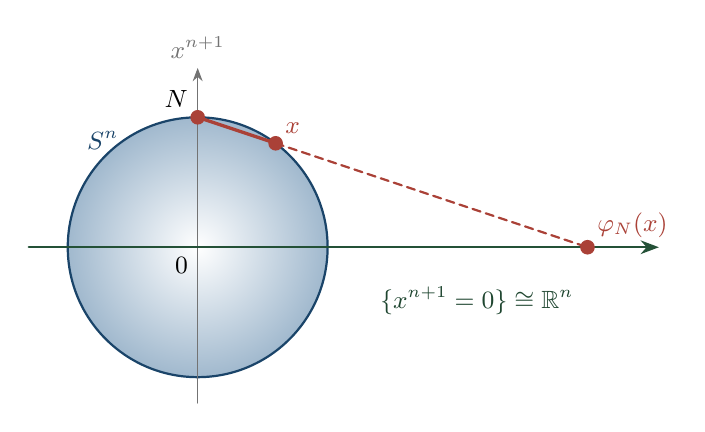
\begin{tikzpicture}[>=Stealth,scale=1.65,line cap=round,line join=round]
\shade[inner color=white,outer color=manifoldblue!43] (0,0) circle (1);
\draw[manifoldblue!75!black,thick] (0,0) circle (1);
\draw[->,black!55] (0,-1.2)--(0,1.38) node[above,font=\small] {$x^{n+1}$};
\draw[->,manifoldgreen!65!black,thick] (-1.3,0)--(3.55,0);
\node[below,font=\small,manifoldgreen!55!black] at (2.15,-.23)
 {$\{x^{n+1}=0\}\cong\R^n$};
\coordinate (N) at (0,1);
\coordinate (X) at (.6,.8);
\coordinate (P) at (3,0);
\draw[manifoldred,very thick] (N)--(X);
\draw[manifoldred,thick,densely dashed] (X)--(P);
\foreach \name in {N,X,P}{\fill[manifoldred] (\name) circle (1.6pt);}
\node[above left,font=\small] at (N) {$N$};
\node[above right,font=\small,manifoldred] at (X) {$x$};
\node[above right,font=\small,manifoldred] at (P) {$\varphi_N(x)$};
\node[below left,font=\small] at (0,0) {$0$};
\node[manifoldblue!75!black,font=\small] at (-.73,.82) {$S^n$};
\end{tikzpicture}
\caption{Rzut stereograficzny na płaszczyznę równikową, zgodny ze wzorem
w tekście. Pokazano przekrój płaszczyzną zawierającą oś biegunową
i punkt $x$. Punkty $N,x,\varphi_N(x)$ leżą na jednej prostej;
punkt przecięcia z $\{x^{n+1}=0\}$ ma współrzędne
$\varphi_N(x)=(x^1,\ldots,x^n)/(1-x^{n+1})$.}
\label{fig:stereo}
\end{figure}


\begin{przyklad}[Rzeczywista przestrzeń rzutowa]\label{prz:RPn}
Niech $\R_*:=\R\setminus\{0\}$ oznacza zbiór niezerowych
liczb rzeczywistych.
Niech $\mathbb{RP}^n = (\R^{n+1}\setminus\{0\})/\!\sim$,
gdzie
\[
x\sim y
\iff
\exists\,\lambda\in\R_*
\quad\text{takie, że}\quad
x=\lambda y.
\]
Przestrzeń $\mathbb{RP}^n$ wyposażamy w topologię ilorazową względem
rzutowania
\[
\pi:\R^{n+1}\setminus\{0\}\longrightarrow\mathbb{RP}^n,
\qquad
\pi(x)=[x].
\]
Punkty przestrzeni rzutowej zapisujemy w postaci $[x^0:\dots:x^n]$.

Dla $i=0,\dots,n$ definiujemy $U_i = \{[x^0:\dots:x^n]\in\mathbb{RP}^n:x^i\neq0\}$.
Najpierw należy sprawdzić, że definicja ta nie zależy od wyboru
reprezentanta klasy $[x]$. Jeżeli $x\sim y$, to istnieje
$\lambda\neq0$ takie, że $y=\lambda x$, a więc $y^i=\lambda x^i$.
Ponieważ $\lambda\neq0$, mamy $x^i\neq0 \iff y^i\neq0$.
Warunek $x^i\neq0$ zależy zatem wyłącznie od klasy $[x]$, więc zbiór
$U_i$ jest dobrze określony.

Zauważmy następnie, że $\pi^{-1}(U_i) = \{x\in\R^{n+1}\setminus\{0\}:x^i\neq0\}$.
Jest to zbiór otwarty w $\R^{n+1}\setminus\{0\}$, ponieważ jest
przeciwobrazem otwartego zbioru
$\R_*$ przez ciągłą funkcję współrzędnościową $x\longmapsto x^i$.
Z definicji topologii ilorazowej zbiór $A\subseteq\mathbb{RP}^n$
jest otwarty wtedy i tylko wtedy, gdy $\pi^{-1}(A)$ jest otwarty
w $\R^{n+1}\setminus\{0\}$. Stąd każdy $U_i$ jest otwarty.

Ponieważ każdy niezerowy wektor
$x=(x^0,\dots,x^n)$ ma przynajmniej jedną niezerową współrzędną,
zbiory $U_i$ pokrywają całą przestrzeń:
\[
\mathbb{RP}^n
=
\bigcup_{i=0}^n U_i.
\]

Na $U_i$ definiujemy odwzorowanie $\varphi_i:U_i\longrightarrow\R^n$
wzorem
\[
\varphi_i([x^0:\dots:x^n])
=
\left(
\frac{x^0}{x^i},
\dots,
\frac{x^{i-1}}{x^i},
\frac{x^{i+1}}{x^i},
\dots,
\frac{x^n}{x^i}
\right),
\]
czyli po znormalizowaniu reprezentanta tak, aby jego $i$-ta
współrzędna była równa $1$, pomijamy tę współrzędną.

Także tutaj należy sprawdzić niezależność od wyboru reprezentanta.
Jeżeli $y=\lambda x$ dla pewnego $\lambda\neq0$, to dla każdego
$j\neq i$ mamy $\frac{y^j}{y^i} = \frac{\lambda x^j}{\lambda x^i} = \frac{x^j}{x^i}$.
Wartość $\varphi_i([x])$ zależy więc wyłącznie od klasy $[x]$.

Odwzorowanie odwrotne jest dane jawnie przez wstawienie $1$
na $i$-te miejsce:
\[
\varphi_i^{-1}
(u^0,\dots,u^{i-1},u^{i+1},\dots,u^n)
=
[u^0:\dots:u^{i-1}:1:u^{i+1}:\dots:u^n].
\]
W szczególności $\varphi_i$ jest bijekcją.

Odwrotność $\varphi_i^{-1}$ jest ciągła, ponieważ jest złożeniem
ciągłego odwzorowania
\[
(u^0,\dots,u^{i-1},u^{i+1},\dots,u^n)
\longmapsto
(u^0,\dots,u^{i-1},1,u^{i+1},\dots,u^n)
\]
z ciągłym rzutowaniem ilorazowym $\pi$.

Aby wykazać ciągłość $\varphi_i$, zauważmy, że na zbiorze $\pi^{-1}(U_i)=\{x^i\neq0\}$
mamy
\[
\varphi_i\circ\pi(x)
=
\left(
\frac{x^0}{x^i},
\dots,
\frac{x^{i-1}}{x^i},
\frac{x^{i+1}}{x^i},
\dots,
\frac{x^n}{x^i}
\right),
\]
a więc $\varphi_i\circ\pi$ jest ciągłe. Ponieważ obcięcie $\pi|_{\pi^{-1}(U_i)}: \pi^{-1}(U_i)\longrightarrow U_i$
jest odwzorowaniem ilorazowym, wynika stąd ciągłość $\varphi_i$.
Otrzymujemy zatem homeomorfizm $\varphi_i:U_i\longrightarrow\R^n$.

Pozostaje sprawdzić zgodność map. Dla $i\neq j$ na przecięciu
$U_i\cap U_j$ odwzorowanie przejścia $\varphi_j\circ\varphi_i^{-1}$
jest określone tam, gdzie współrzędna odpowiadająca ilorazowi
$x^j/x^i$ jest niezerowa. Każda jego składowa jest albo odwrotnością
tej współrzędnej, albo ilorazem jednej ze współrzędnych przez nią.
Są to zatem funkcje wymierne o nieznikającym na dziedzinie
mianowniku, a więc funkcje gładkie.

W konsekwencji $\{(U_i,\varphi_i)\}_{i=0}^n$
jest atlasem gładkim. Po sprawdzeniu aksjomatów topologicznych
w twierdzeniu poniżej otrzymujemy, że $\mathbb{RP}^n$ jest
rozmaitością gładką wymiaru $n$.
\end{przyklad}


\begin{przyklad}[Dwie mapy $\mathbb{RP}^2$ krok po kroku]\label{prz:RP2-przejscie-1}
Na $U_0$ każda klasa ma jednoznacznego reprezentanta $[1:u:v]$,
natomiast na $U_1$ ma reprezentanta $[a:1:b]$.
Ich część wspólna $U_0\cap U_1$, zapisana we współrzędnych mapy
$\varphi_0$, odpowiada warunkowi $u\neq0$. Aby przejść od współrzędnych
zadanych przez $\varphi_0$ do współrzędnych zadanych przez $\varphi_1$,
dzielimy trzy współrzędne jednorodne przez $u$: $[1:u:v] = [1/u:1:v/u]$.
Stąd odwzorowanie zmiany współrzędnych ma postać $\varphi_1\circ\varphi_0^{-1}(u,v) = \left(\frac1u,\frac vu\right)$.
Oznacza to, że jeżeli punkt $p\in U_0\cap U_1$ ma w pierwszej mapie
współrzędne $\varphi_0(p)=(u,v)$,
to w drugiej mapie jego współrzędne wynoszą $\varphi_1(p)=(a,b) = \left(\frac1u,\frac vu\right)$.

Dziedziną odwzorowania przejścia jest $\{(u,v)\in\R^2:u\neq0\}$,
a jego macierz Jacobiego wynosi
\[
D(\varphi_1\circ\varphi_0^{-1})(u,v)
=
\begin{pmatrix}
-u^{-2} & 0\\[1mm]
-vu^{-2} & u^{-1}
\end{pmatrix}.
\]
Ponieważ $\det D(\varphi_1\circ\varphi_0^{-1})(u,v) = -u^{-3}\neq0$,
a odwrotne przejście ma postać $(a,b)\longmapsto \left(\frac1a,\frac ba\right)$,
odwzorowanie przejścia jest dyfeomorfizmem.

Zmianę współrzędnych wektora stycznego w tych mapach obliczymy
w przykładzie~\ref{prz:RP2-styczna-1}, po zdefiniowaniu przestrzeni stycznej.
\end{przyklad}


\begin{uwaga}[Geometryczna interpretacja $\mathbb{RP}^1$ i $\mathbb{RP}^2$]
Przestrzeń $\mathbb{RP}^n$ można interpretować jako zbiór prostych
przechodzących przez początek układu współrzędnych w $\R^{n+1}$.
Rzeczywiście, punkt $[x^0:\dots:x^n]\in\mathbb{RP}^n$
odpowiada prostej $\ell_x=\{\lambda x:\lambda\in\R\}$.
Zmiana reprezentanta $x$ na $\mu x$, gdzie $\mu\neq0$, nie zmienia tej
prostej. Współrzędne jednorodne opisują więc nie konkretny punkt
$\R^{n+1}$, lecz kierunek prostej przechodzącej przez $0$.

Każda taka prosta przecina sferę jednostkową $S^n$ w dokładnie dwóch
punktach antypodalnych $x$ i $-x$. Stąd $\mathbb{RP}^n\cong S^n/\{x\sim-x\}$.
Jest to także identyfikacja topologii. Oznaczmy pierwotne rzutowanie
przez $\pi$ i jego ograniczenie do sfery przez $q$.
Normalizacja $\nu(x)=x/\|x\|$ jest ciągła i $\pi=q\circ\nu$.
Jeśli $q^{-1}(A)$ jest otwarty w sferze, to
$\pi^{-1}(A)=\nu^{-1}(q^{-1}(A))$ jest otwarty, zatem $A$ jest
otwarty w pierwotnej topologii ilorazowej. Odwrotna implikacja
wynika z ciągłości $q$. Stąd $q$ jest odwzorowaniem ilorazowym,
co uzasadnia powyższy homeomorfizm.

Dla $n=1$ otrzymujemy $\mathbb{RP}^1\cong S^1/\{z\sim-z\}$.
Po utożsamieniu $S^1$ z okręgiem jednostkowym w $\C$ rozważmy
odwzorowanie $F:S^1\to S^1,\ F(z)=z^2$.
Ponieważ $F(z)=F(-z)$,
odwzorowanie to jest stałe na parach antypodalnych i wyznacza
odwzorowanie $\widetilde F:\mathbb{RP}^1\to S^1, \ \widetilde F([z])=z^2$.
Jest ono bijekcją, ponieważ $z^2=w^2 \iff z=\pm w$,
a każdy punkt okręgu posiada dwa przeciwne pierwiastki kwadratowe.
Ciągłość $\widetilde F$ wynika z ciągłości $F=\widetilde F\circ q$
i własności ilorazu. Ponieważ $\mathbb{RP}^1=q(S^1)$ jest zwarta,
a $S^1$ jest przestrzenią Hausdorffa, $\widetilde F$ jest homeomorfizmem.

Jest to również dyfeomorfizm. Jeśli $z=e^{i\theta}$,
to w $\mathbb{RP}^1$ kąty $\theta$ i $\theta+\pi$ opisują ten sam punkt,
natomiast $\widetilde F([e^{i\theta}])=e^{2i\theta}$.
Sprawdźmy zgodność współrzędnych kątowych z podanym wcześniej atlasem.
Dla $[\cos\theta:\sin\theta]$, na małym przedziale z $\cos\theta\ne0$,
współrzędną afiniczną jest $\tan\theta$, o pochodnej $1/\cos^2\theta$.
Gdy $\sin\theta\ne0$, druga mapa daje $\cot\theta$, o pochodnej
$-1/\sin^2\theta$. Pochodne nie znikają, więc przejścia i ich lokalne
odwrotności są gładkie. Kąt jest zatem zgodną lokalną współrzędną.
W lokalnych współrzędnych kątowych odwzorowanie ma więc postać $\theta\longmapsto 2\theta$,
a jego lokalna odwrotność $\alpha\longmapsto \frac{\alpha}{2}$.
Oba odwzorowania są gładkie, zatem $\mathbb{RP}^1\cong S^1$
jako rozmaitości gładkie.

Dla $n=2$ otrzymujemy $\mathbb{RP}^2\cong S^2/\{x\sim-x\}$.
Możemy ograniczyć się do domkniętej półsfery północnej. Każda para
antypodalna spoza równika ma dokładnie jeden punkt w jej wnętrzu; na równiku
oba punkty pary należą do półsfery. Ponieważ domknięta półsfera jest
homeomorficzna z dyskiem $D^2$, otrzymujemy model $\mathbb{RP}^2 \cong D^2/\{x\sim-x\text{ dla }x\in\partial D^2\}$.
Oznacza to, że punkty wewnętrzne dysku pozostają różne, natomiast każdy
punkt brzegu utożsamiamy z punktem antypodalnym. Rzutowanie półsfery
na $\mathbb{RP}^2$ jest ciągłą surjekcją i ma dokładnie te włókna.
Wyznacza zatem ciągłą bijekcję z opisanego ilorazu dysku.
Jej dziedzina jest zwarta, a $\mathbb{RP}^2$ jest przestrzenią Hausdorffa
na mocy twierdzenia~\ref{thm:rzutowe-zwarte-1}; jest więc homeomorfizmem.

Model ten daje również intuicję, dlaczego $\mathbb{RP}^2$ nie jest
orientowalna. Wyobraźmy sobie małą strzałkę lub niewielką figurę
asymetryczną przesuwaną po dysku. Gdy dochodzimy do brzegu, przechodzimy
przez niego dzięki utożsamieniu z punktem leżącym po przeciwnej stronie
okręgu. Po takim przejściu kierunek wzdłuż brzegu pozostaje zgodny,
natomiast kierunek wskazujący do wnętrza dysku zostaje odwrócony.

Lokalnie można to zapisać schematycznie jako $(s,t)\longmapsto (s,-t)$,
gdzie $s$ oznacza kierunek wzdłuż brzegu, a $t$ kierunek poprzeczny.
Jedna z dwóch lokalnych współrzędnych zmienia więc zwrot. Po przejściu
wzdłuż odpowiedniej zamkniętej drogi wracamy do punktu początkowego
z odwróconą lokalną orientacją. Nie można zatem wybrać orientacji
w sposób zgodny na całej przestrzeni.

Jest to geometryczna intuicja nieorientowalności $\mathbb{RP}^2$;
formalny dowód podamy po wprowadzeniu pojęcia orientacji rozmaitości.
\end{uwaga}


\begin{figure}[h]
\centering
\begin{tikzpicture}[>=Stealth,scale=1]

  %-------------------- RP^1 --------------------
  \begin{scope}
    % Okrąg
    \draw[thick,manifoldblue] (0,0) circle (1.45);

    % Kilka par antypodalnych na okręgu
    \foreach \ang in {0,45,90,135}{
        \draw[dashed,gray!55]
            (\ang:1.45) -- ({\ang+180}:1.45);

        \fill[manifoldgold]
            (\ang:1.45) circle (2.2pt);
        \fill[manifoldgold]
            ({\ang+180}:1.45) circle (2.2pt);
    }

    % Wyróżniona para x i -x
    \fill[manifoldred] (20:1.45) circle (2.8pt);
    \fill[manifoldred] (200:1.45) circle (2.8pt);

    \node[manifoldred, above right] at (20:1.45) {$x$};
    \node[manifoldred, below left] at (200:1.45) {$-x$};

    % Strzałka pokazująca utożsamienie wyróżnionej pary
    \draw[<->,thick,manifoldred]
      (20:1.36) to[bend left=18] (200:1.36);

    % Opisy
    \node[manifoldblue] at (0,1.85) {$S^1$};

    \node[align=center,manifoldred] at (0,-1.95)
      {$x\sim -x$ dla każdego $x\in S^1$};

    \node at (0,-2.35)
      {$\displaystyle \mathbb{RP}^1\cong S^1/\{x\sim -x\}$};

    \node at (0,-2.75)
      {$\displaystyle \cong\, S^1$};
  \end{scope}

  %-------------------- RP^2 --------------------
  \begin{scope}[xshift=6.2cm]
    % Dysk
    \fill[manifoldblue!8] (0,0) circle (1.45);
    \draw[thick,manifoldblue] (0,0) circle (1.45);

    % Kilka przykładowych par punktów antypodalnych na brzegu
    \foreach \ang in {0,45,90,135}{
        \fill[manifoldgold]
            (\ang:1.45) circle (2.2pt);
        \fill[manifoldgold]
            ({\ang+180}:1.45) circle (2.2pt);
    }

    % Wyróżniona para x i -x
    \fill[manifoldred] (0:1.45) circle (2.8pt);
    \fill[manifoldred] (180:1.45) circle (2.8pt);

    \node[manifoldred, right] at (0:1.45) {$x$};
    \node[manifoldred, left]  at (180:1.45) {$-x$};

    % Strzałka pokazująca utożsamienie
    \draw[<->,thick,manifoldred]
        (1.36,0) to[bend left=20] (-1.36,0);
    \node[align=center,font=\scriptsize,manifoldblue] at (0,0.55)
        {wnętrze bez\\utożsamień};

    % Opisy
    \node[manifoldblue] at (0,1.85) {$D^2$};

    \node[align=center,manifoldred] at (0,-1.95)
        {$x\sim -x$ dla każdego $x\in\partial D^2$};

    \node at (0,-2.35)
        {$\displaystyle \mathbb{RP}^2
        \cong D^2/\{x\sim -x,\;x\in\partial D^2\}$};
  \end{scope}

\end{tikzpicture}
\caption{Dwa użyteczne modele przestrzeni rzutowych.
Po lewej, $\mathbb{RP}^1$ otrzymujemy z okręgu $S^1$ przez utożsamienie
par antypodalnych punktów. Po prawej, $\mathbb{RP}^2$ otrzymujemy z dysku
$D^2$ przez utożsamienie antypodalnych punktów jego brzegu. Różnica polega
na tym, że w pierwszym przypadku utożsamiamy punkty na całym okręgu,
natomiast w drugim utożsamienie zachodzi tylko na brzegu dysku.}
\label{fig:projective-models}
\end{figure}


\begin{twierdzenie}[Przestrzenie rzutowe jako zwarte rozmaitości]\label{thm:rzutowe-zwarte-1}
Przestrzeń $\mathbb{RP}^n$ jest zwartą rozmaitością gładką wymiaru $n$, a
$\mathbb{CP}^n$ jest zwartą rozmaitością zespoloną wymiaru $n$ (a więc zwartą
rozmaitością rzeczywistą wymiaru $2n$).
\end{twierdzenie}

\begin{proof}
Zaczniemy od zwartości. Niech
\[
\pi_{\R}:\R^{n+1}\setminus\{0\}\longrightarrow\mathbb{RP}^n,
\qquad
\pi_{\R}(x)=[x],
\]
będzie rzutowaniem ilorazowym. Ograniczając je do sfery jednostkowej,
otrzymujemy ciągłe odwzorowanie $q_{\R}:S^n\longrightarrow\mathbb{RP}^n, \ q_{\R}(x)=[x]$.
Jest ono surjektywne. Istotnie, jeśli $[x]\in\mathbb{RP}^n$,
to $x\neq0$ i możemy znormalizować reprezentanta: $\widehat{x}:=\frac{x}{\|x\|}\in S^n$.
Ponieważ $\widehat{x}$ jest niezerową wielokrotnością $x$, mamy $[\widehat{x}]=[x]$.
Każdy punkt $\mathbb{RP}^n$ należy więc do obrazu $q_{\R}$.

Sfera $S^n$ jest zwarta, a ciągły obraz przestrzeni zwartej jest zwarty.
Ponieważ $q_{\R}(S^n)=\mathbb{RP}^n$,
otrzymujemy, że $\mathbb{RP}^n$ jest zwarta.

Dokładnie ten sam argument działa w przypadku zespolonym. Niech
\[
\pi_{\C}:\C^{n+1}\setminus\{0\}\longrightarrow\mathbb{CP}^n,
\qquad
\pi_{\C}(z)=[z].
\]
Po utożsamieniu $\C^{n+1}\cong\R^{2n+2}$ sfera jednostkowa ma postać $S^{2n+1} = \{z\in\C^{n+1}:\|z\|=1\}$.
Ograniczenie $q_{\C}:S^{2n+1}\longrightarrow\mathbb{CP}^n, \ q_{\C}(z)=[z]$,
jest ciągłe i surjektywne, ponieważ dla każdego $[z]\in\mathbb{CP}^n$
wektor $\widehat{z}:=\frac{z}{\|z\|}$
należy do $S^{2n+1}$ i reprezentuje tę samą klasę: $[\widehat{z}]=[z]$.
Ponieważ $S^{2n+1}$ jest zwarta, jej ciągły obraz $q_{\C}(S^{2n+1})=\mathbb{CP}^n$
jest zwarty. Zatem również $\mathbb{CP}^n$ jest zwarta.

Sprawdźmy teraz aksjomat Hausdorffa bez powoływania się na ogólne
twierdzenie o ilorazach. Dla jednostkowych reprezentantów $x,y\in S^n$
dwóch klas rzeczywistych połóżmy $d_{\R}([x],[y]) = \min\{\|x-y\|,\|x+y\|\}$.
Dla jednostkowych reprezentantów $z,w\in S^{2n+1}$ połóżmy $d_{\C}([z],[w]) = \min_{|\lambda|=1}\|z-\lambda w\|$.
Oba wzory nie zależą od wyboru jednostkowych reprezentantów:
w przypadku rzeczywistym zmiana $x$ na $-x$ jedynie zamienia miejscami
dwie liczby występujące w minimum, natomiast w przypadku zespolonym
zmiana reprezentanta przez czynnik o module $1$ jedynie zmienia
parametryzację zbioru, po którym bierzemy minimum. Minima istnieją
dzięki zwartości grup $\{\pm1\}$ i $S^1$.

Nierówność trójkąta sprawdzimy jednocześnie dla obu przypadków,
pisząc $G=\{\pm1\}$ lub $G=S^1$. Dla jednostkowych $x,y,z$
wybierzmy $\lambda,\mu\in G$ realizujące minima dla par $(x,y)$ i $(y,z)$.
Ponieważ mnożenie przez $\lambda$ zachowuje normę,
\begin{align*}
d([x],[z])&\leq\|x-\lambda\mu z\|\\
&\leq\|x-\lambda y\|+\|\lambda y-\lambda\mu z\|\\
&=d([x],[y])+d([y],[z]).
\end{align*}
Symetria wynika z zastąpienia $\lambda$ przez $\lambda^{-1}$.
Ponadto osiągane minimum jest równe zeru wtedy i tylko wtedy,
gdy reprezentanty należą do tej samej orbity, czyli reprezentują
ten sam punkt przestrzeni rzutowej. Otrzymujemy więc metryki na zbiorach klas.

Pozostaje sprawdzić, że topologie wyznaczone przez te metryki są
topologiami ilorazowymi. Rzutowania
\[
q_{\R}:S^n\to(\mathbb{RP}^n,d_{\R}),
\qquad
q_{\C}:S^{2n+1}\to(\mathbb{CP}^n,d_{\C})
\]
są ciągłe, ponieważ odległość klas nie przekracza odległości ich
wybranych reprezentantów. Aby przejść od sfer do pierwotnych ilorazów,
używamy ciągłej normalizacji $\nu(v)=v/\|v\|$.
Rzutowania $\pi_{\R}$ i $\pi_{\C}$ do przestrzeni klas z metryką są ciągłe,
bo mają postać $q_{\R}\circ\nu$ i $q_{\C}\circ\nu$.
Z definicji topologii ilorazowej wynika więc ciągłość identyczności
z pierwotnego ilorazu do przestrzeni metrycznej.
Z drugiej strony mamy już wykazaną zwartość
$\mathbb{RP}^n$ i $\mathbb{CP}^n$ w ich topologiach ilorazowych.
Identyczność z przestrzeni rzutowej wyposażonej w topologię ilorazową
do tego samego zbioru klas wyposażonego w powyższą metrykę jest więc
ciągłą bijekcją ze zwartej przestrzeni do przestrzeni Hausdorffa.
Jest zatem homeomorfizmem. W szczególności pierwotna topologia
ilorazowa jest Hausdorffa.

Każda z przestrzeni rzutowych ma skończony atlas $U_0,\ldots,U_n$,
którego obrazy są równe odpowiednio $\R^n$ lub $\C^n$. Wybierzmy
w $\R^n$ oraz $\C^n\cong\R^{2n}$ przeliczalną bazę, na przykład
złożoną z kul o wymiernych środkach i wymiernych promieniach.
Przeciwobrazy tych baz przez skończenie wiele map atlasu tworzą
przeliczalną bazę przestrzeni rzutowej.

Odwzorowania przejścia są ilorazami współrzędnych przez współrzędną
niezerową, a więc są gładkie w przypadku rzeczywistym i holomorficzne
w przypadku zespolonym. Otrzymujemy zatem strukturę rozmaitości
gładkiej wymiaru $n$ na $\mathbb{RP}^n$ oraz strukturę rozmaitości
zespolonej wymiaru $n$ na $\mathbb{CP}^n$. Ponieważ $\C^n\cong\R^{2n}$,
$\mathbb{CP}^n$ ma jako rozmaitość rzeczywista wymiar $2n$.
\end{proof}


\begin{uwaga}
Zwartość można zobaczyć bardzo bezpośrednio: każde $\mathbb{RP}^n$ jest ilorazem
sfery $S^n$ przez relację $x\sim-x$, a $\mathbb{CP}^n$ jest ilorazem sfery
jednostkowej $S^{2n+1}\subset\C^{n+1}$ przez działanie grupy $S^1$, $z\sim e^{i\theta}z$.
W przypadku zespolonym otrzymujemy w ten sposób słynne rozwłóknienie Hopfa
$S^1\longrightarrow S^{2n+1}\longrightarrow\mathbb{CP}^n$.
Pełny opis tej konstrukcji wykracza poza zakres tego rozdziału, ale pokazuje,
że przestrzenie rzutowe są naturalnie związane zarówno z ilorazami, jak i z teorią
wiązek.
\end{uwaga}

\begin{przyklad}[Torus $T^n$]\label{prz:torus}
Niech $T^n=\R^n/\Z^n$ z topologią ilorazową względem rzutowania kanonicznego $\pi\colon\R^n
\to T^n$, $\pi(x)=x+\Z^n$. Pokażemy najpierw, że $\pi$ jest odwzorowaniem otwartym: dla
zbioru otwartego $\Omega\subseteq\R^n$, $\pi^{-1}(\pi(\Omega))=\bigcup_{k\in\Z^n}(\Omega+k)$
jest sumą zbiorów otwartych, a więc otwarty; z definicji topologii ilorazowej oznacza to,
że $\pi(\Omega)$ jest otwarty w $T^n$.

Sprawdźmy pozostałe warunki topologiczne. Jeśli $[x]\ne[y]$, to
$\delta=\inf_{k\in\Z^n}\|x-y-k\|>0$: w dowolnym ograniczonym
zbiorze jest tylko skończenie wiele punktów kraty, a $x-y\notin\Z^n$.
Otwarte otoczenia $\pi(B(x,\delta/3))$ i $\pi(B(y,\delta/3))$
są rozłączne. W przeciwnym razie istniałyby $u,v$ w tych kulach
z $u-v=k\in\Z^n$, skąd $\|x-y-k\|<2\delta/3$, sprzeczność.
Torus jest więc Hausdorffa. Obrazy przeliczalnej bazy kul w $\R^n$
stanowią bazę ilorazu: dla otwartego $O\subset T^n$ i $[x]\in O$
wybieramy kulę bazową $B$ z $x\in B\subset\pi^{-1}(O)$;
wtedy $[x]\in\pi(B)\subset O$. To daje drugi aksjomat przeliczalności.

Niech $B(x,1/2)\subseteq\R^n$ będzie kulą otwartą o promieniu $1/2$. Dla $k\in\Z^n\setminus
\{0\}$, zbiory $B(x,1/2)$ i $B(x+k,1/2)$ są rozłączne: gdyby $y$ należał do obu, to
$\|y-x\|<1/2$ i $\|y-x-k\|<1/2$, skąd z nierówności trójkąta $\|k\|\leq\|y-x\|+\|y-x-k\|<1$;
ale $\|k\|\geq1$ dla $k\in\Z^n\setminus\{0\}$ — sprzeczność. Zatem $\pi|_{B(x,1/2)}$ jest
różnowartościowe, a więc — jako odwzorowanie ciągłe, otwarte i różnowartościowe na obraz —
homeomorfizmem $B(x,1/2)\to\pi(B(x,1/2))$. Kładziemy $\varphi_x:=(\pi|_{B(x,1/2)})^{-1}$;
zbiory $\pi(B(x,1/2))$ dla $x\in\R^n$ pokrywają $T^n$.

Odwzorowania przejścia między takimi mapami są (lokalnie) postaci $y\mapsto y+k$ dla
pewnego ustalonego $k\in\Z^n$ (bo dwa punkty z tym samym obrazem przy $\pi$ różnią się
dokładnie o wektor z $\Z^n$, a $k$ jest lokalnie stałe z ciągłości) — a translacja jest
odwzorowaniem gładkim z gładką odwrotną. Zatem otrzymana rodzina map jest atlasem, i $T^n$
jest rozmaitością gładką wymiaru $n$.
\end{przyklad}
\section{Przestrzeń styczna}\label{sec:przestrzen-styczna}

W porównaniu trzech poniższych modeli zakładamy,
że $M$ nie ma brzegu. Dla punktów brzegu
przestrzeń styczną definiujemy przez derywacje
lub współrzędne przedłużane poza półprzestrzeń,
jak w Sekcji~\ref{sec:rozmaitosci-z-brzegiem-1};
model dwustronnych krzywych nie działa tam dosłownie.

Chcemy nadać sens pojęciu ,,wektora stycznego'' do rozmaitości $M$ w punkcie $p$ —
uogólnieniu intuicji wektora stycznego do powierzchni w $\R^3$, niezależnemu od
zanurzenia $M$ w jakąkolwiek przestrzeń otaczającą. Istnieje kilka naturalnych, a priori
różnych, sposobów sformalizowania tej intuicji; w tej sekcji podajemy trzy z nich i
dowodzimy, że są one kanonicznie równoważne.

\subsection*{Trzy definicje przestrzeni stycznej}

Niech $M$ będzie rozmaitością gładką wymiaru $n$, $p\in M$.

\paragraph*{Definicja A (poprzez krzywe).} Niech $\Gamma_p$ oznacza zbiór gładkich krzywych
$\gamma\colon(-\varepsilon,\varepsilon)\to M$ (dla pewnego $\varepsilon>0$, zależnego od
$\gamma$) z $\gamma(0)=p$. Mówimy, że $\gamma_1,\gamma_2\in\Gamma_p$ są \emph{styczne w
$p$}, $\gamma_1\sim\gamma_2$, jeśli dla pewnej (równoważnie: każdej) mapy dopuszczalnej
$(U,\varphi)$ wokół $p$,
\[
(\varphi\circ\gamma_1)'(0)=(\varphi\circ\gamma_2)'(0)\quad\text{w }\R^n.
\]

\begin{figure}[!ht]
\centering
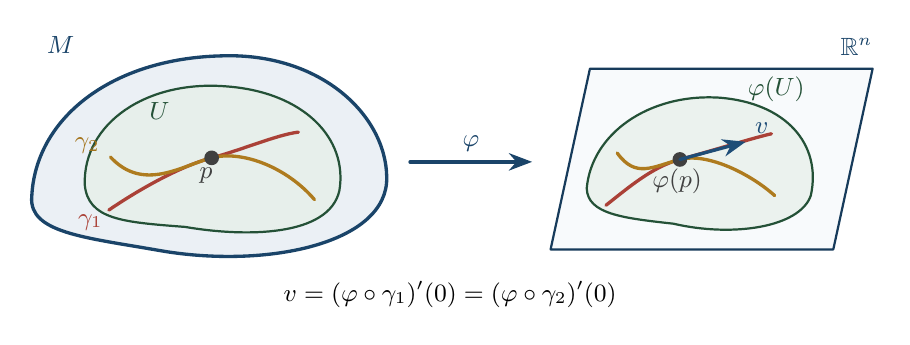
\begin{tikzpicture}[>=Stealth,scale=1.02,line cap=round,line join=round]
% Dwie różne krzywe, których pochodne w p po przejściu do współrzędnych są równe.
\filldraw[fill=manifoldblue!9,draw=manifoldblue!75!black,very thick]
 (-5.04,-.52) .. controls (-5.0,.46) and (-4.05,1.21) .. (-2.67,1.24)
 .. controls (-1.44,1.28) and (-.63,.5) .. (-.62,-.27)
 .. controls (-.6,-1.1) and (-2.13,-1.42) .. (-3.47,-1.18)
 .. controls (-4.39,-1.02) and (-5.07,-.96) .. cycle;
\filldraw[fill=manifoldgreen!12,draw=manifoldgreen!65!black,thick]
 (-4.38,-.36) .. controls (-4.4,.4) and (-3.61,.94) .. (-2.62,.86)
 .. controls (-1.65,.79) and (-1.1,.21) .. (-1.21,-.44)
 .. controls (-1.34,-1.01) and (-2.37,-1.02) .. (-3.13,-.89)
 .. controls (-3.91,-.83) and (-4.34,-.8) .. cycle;
\node[font=\small\bfseries,manifoldblue!75!black] at (-4.68,1.37) {$M$};
\node[font=\small,manifoldgreen!65!black] at (-3.45,.55) {$U$};
\draw[manifoldred,very thick]
 (-4.08,-.68) .. controls (-3.7,-.42) and (-3.18,-.13) .. (-2.8,-.03)
 .. controls (-2.42,.07) and (-1.98,.26) .. (-1.72,.29);
\draw[manifoldgold!85!black,very thick]
 (-4.06,-.02) .. controls (-3.65,-.46) and (-3.18,-.13) .. (-2.8,-.03)
 .. controls (-2.42,.07) and (-1.86,-.15) .. (-1.52,-.55);
\node[font=\small,manifoldred] at (-4.31,-.83) {$\gamma_1$};
\node[font=\small,manifoldgold!80!black] at (-4.35,.12) {$\gamma_2$};
\fill[black!75] (-2.8,-.03) circle (2.6pt)
 node[below,font=\small,xshift=-2pt] {$p$};
\draw[->,very thick,manifoldblue!75!black] (-.33,-.08)--(1.19,-.08)
 node[midway,above,font=\small] {$\varphi$};
% Rysunkowy fragment R^n oraz obraz U.
\filldraw[fill=manifoldblue!3,draw=manifoldblue!65!black,thick]
 (1.42,-1.17)--(4.94,-1.17)--(5.43,1.08)--(1.91,1.08)--cycle;
\filldraw[fill=manifoldgreen!10,draw=manifoldgreen!65!black,thick]
 (1.87,-.41) .. controls (1.93,.27) and (2.64,.77) .. (3.51,.72)
 .. controls (4.35,.66) and (4.8,.14) .. (4.66,-.5)
 .. controls (4.52,-.9) and (3.68,-1.02) .. (2.95,-.85)
 .. controls (2.32,-.78) and (1.88,-.73) .. cycle;
\draw[manifoldred,very thick]
 (2.11,-.62) .. controls (2.39,-.4) and (2.69,-.14) .. (3.03,-.05)
 .. controls (3.37,.04) and (3.91,.21) .. (4.17,.27);
\draw[manifoldgold!85!black,very thick]
 (2.25,.03) .. controls (2.48,-.29) and (2.69,-.14) .. (3.03,-.05)
 .. controls (3.37,.04) and (3.91,-.23) .. (4.21,-.5);
\fill[black!75] (3.03,-.05) circle (2.6pt)
 node[below,font=\small,xshift=-1pt] {$\varphi(p)$};
\draw[->,very thick,manifoldblue!85!black] (3.03,-.05)--(3.85,.17);
\node[font=\small,manifoldblue!85!black] at (4.05,.34) {$v$};
\node[font=\small,manifoldgreen!65!black] at (4.23,.82) {$\varphi(U)$};
\node[font=\small\bfseries,manifoldblue!75!black] at (5.23,1.35) {$\R^n$};
\node[font=\small] at (.17,-1.73)
 {$v=(\varphi\circ\gamma_1)'(0)=(\varphi\circ\gamma_2)'(0)$};
\end{tikzpicture}
\caption{Dwie krzywe w $M$ przechodzą przez $p$ i mają ten sam kierunek
styczny. W mapie $\varphi$ ich obrazy mają wspólną pochodną $v$ w $t=0$.}
\label{fig:krzywe-styczne-w-mapie}
\end{figure}

\begin{fakt}
Powyższy warunek nie zależy od wyboru mapy $(U,\varphi)$.
\end{fakt}
\begin{proof}
Jeśli $(V,\psi)$ jest inną mapą wokół $p$, to na wspólnej dziedzinie $\psi\circ\gamma_i=
(\psi\circ\varphi^{-1})\circ(\varphi\circ\gamma_i)$ blisko $t=0$, więc z reguły łańcucha
\[
(\psi\circ\gamma_i)'(0)=D(\psi\circ\varphi^{-1})(\varphi(p))\cdot(\varphi\circ\gamma_i)'(0),
\qquad i=1,2.
\]
Ponieważ $D(\psi\circ\varphi^{-1})(\varphi(p))$ jest tym samym przekształceniem liniowym
dla $i=1$ i $i=2$, równość $(\varphi\circ\gamma_1)'(0)=(\varphi\circ\gamma_2)'(0)$
implikuje $(\psi\circ\gamma_1)'(0)=(\psi\circ\gamma_2)'(0)$, i na odwrót (bo
$D(\psi\circ\varphi^{-1})(\varphi(p))$ jest odwracalne, jako różniczka dyfeomorfizmu).
\end{proof}

Relacja $\sim$ jest relacją równoważności na $\Gamma_p$ (natychmiast z definicji, poprzez
odpowiednie własności równości w $\R^n$). Definiujemy $T_p^AM:=\Gamma_p/\!\sim$.

Aby wyposażyć $T_p^AM$ w strukturę przestrzeni wektorowej, ustalmy mapę
$(U,\varphi)$ wokół $p$ i zdefiniujmy
\[
\Theta_\varphi:T_p^AM\longrightarrow\R^n,
\qquad
\Theta_\varphi([\gamma]):=(\varphi\circ\gamma)'(0).
\]
Odwzorowanie to jest dobrze określone i bijektywne. Różnowartościowość
wynika bezpośrednio z definicji relacji równoważności, natomiast
surjektywność z faktu, że dla dowolnego $v\in\R^n$ krzywa $\gamma(t)=\varphi^{-1}(\varphi(p)+tv)$,
określona dla dostatecznie małych $|t|$, spełnia $\gamma(0)=p, \ (\varphi\circ\gamma)'(0)=v$.

Za pomocą bijekcji $\Theta_\varphi$ przenosimy strukturę przestrzeni
wektorowej z $\R^n$ na $T_p^AM$, definiując
\[
[\gamma]+[\eta]
:=
\Theta_\varphi^{-1}
\bigl(\Theta_\varphi([\gamma])+\Theta_\varphi([\eta])\bigr)
\]
oraz
\[
a[\gamma]
:=
\Theta_\varphi^{-1}
\bigl(a\,\Theta_\varphi([\gamma])\bigr),
\qquad a\in\R.
\]
W szczególności mnożenie przez skalar można reprezentować przez
reparametryzację krzywej: $a[\gamma]=[t\mapsto\gamma(at)]$,
ponieważ $(\varphi\circ\gamma(at))'_{\,t=0} = a(\varphi\circ\gamma)'(0)$.
W ten sposób $\Theta_\varphi$ jest, z definicji, izomorfizmem liniowym
$T_p^AM\cong\R^n$.

\begin{fakt}
Struktura liniowa na $T_p^AM$ nie zależy od wyboru mapy $\varphi$.
\end{fakt}
\begin{proof}
Niech $(V,\psi)$ będzie inną mapą wokół $p$, $L:=D(\psi\circ\varphi^{-1})(\varphi(p))
\colon\R^n\to\R^n$. Z rachunku w poprzednim Fakcie, dla dowolnej krzywej $\gamma\in\Gamma_p$,
$\Theta_\psi([\gamma])=L(\Theta_\varphi([\gamma]))$, czyli $\Theta_\psi=L\circ\Theta_\varphi$.
Ponieważ $L$ jest izomorfizmem \emph{liniowym} (jako różniczka dyfeomorfizmu w punkcie),
struktury liniowe przeniesione na $T_p^AM$ przez $\Theta_\varphi$ i przez $\Theta_\psi=
L\circ\Theta_\varphi$ pokrywają się: liniowość $L$ gwarantuje, że dla dowolnych $[\gamma_1],
[\gamma_2]\in T_p^AM$, $a,b\in\R$, kombinacja $a[\gamma_1]+b[\gamma_2]$ wyznaczona przez
$\Theta_\varphi$ pokrywa się z kombinacją wyznaczoną przez $\Theta_\psi$. To kluczowa
obserwacja: liniowość różniczki odwzorowania przejścia gwarantuje, że mimo iż
$\Theta_\varphi\neq\Theta_\psi$, wyznaczona przez nie struktura wektorowa na $T_p^AM$ jest
jedna i ta sama.
\end{proof}

\paragraph*{Definicja B (klasyczna, poprzez pary mapa-wektor).} Rozważmy zbiór trójek
$(U,\varphi,v)$, gdzie $(U,\varphi)$ jest mapą dopuszczalną wokół $p$, a $v\in\R^n$.
Mówimy, że $(U,\varphi,v)\sim(V,\psi,w)$, jeśli $w=D(\psi\circ\varphi^{-1})(\varphi(p))\,v$.

\begin{fakt}
Powyższa relacja jest relacją równoważności.
\end{fakt}
\begin{proof}
Zwrotność: dla $\psi=\varphi$, $D(\id)=\id$, więc $v=v$. Symetria: jeśli $w=D(\psi\varphi^{-1})
(\varphi(p))v$, to stosując regułę łańcucha do $\varphi\circ\psi^{-1}=(\psi\circ
\varphi^{-1})^{-1}$ w punkcie $\psi(p)$, $D(\varphi\psi^{-1})(\psi(p))=\big[D(\psi\varphi^{-1})
(\varphi(p))\big]^{-1}$, skąd $v=D(\varphi\psi^{-1})(\psi(p))w$. Przechodniość: jeśli
$w=D(\psi\varphi^{-1})(\varphi(p))v$ i $u=D(\eta\psi^{-1})(\psi(p))w$, to z reguły łańcucha
zastosowanej do $\eta\circ\varphi^{-1}=(\eta\circ\psi^{-1})\circ(\psi\circ\varphi^{-1})$ w
punkcie $\varphi(p)$,
\[
D(\eta\varphi^{-1})(\varphi(p))=D(\eta\psi^{-1})(\psi(p))\cdot D(\psi\varphi^{-1})(\varphi(p)),
\]
a więc $D(\eta\varphi^{-1})(\varphi(p))v=D(\eta\psi^{-1})(\psi(p))w=u$, czyli
$(U,\varphi,v)\sim(W,\eta,u)$.
\end{proof}

Definiujemy $T_p^BM$ jako zbiór klas równoważności $[U,\varphi,v]$.
Strukturę przestrzeni wektorowej wprowadzamy wzorem $a[U,\varphi,v]+b[U,\varphi,v'] := [U,\varphi,av+bv']$.
Definicja ta jest dobrze określona, to znaczy wynik nie zależy od wyboru
reprezentantów klas. Istotnie, jeżeli przejdziemy do innej mapy
$(V,\psi)$ zawierającej punkt $p$, to wektory $v,v'\in\mathbb{R}^n$
przechodzą odpowiednio w
\[
D(\psi\circ\varphi^{-1})(\varphi(p))\,v
\qquad\text{oraz}\qquad
D(\psi\circ\varphi^{-1})(\varphi(p))\,v'.
\]
Z liniowości różniczki otrzymujemy
\[
D(\psi\circ\varphi^{-1})(\varphi(p))(av+bv')
=
a\,D(\psi\circ\varphi^{-1})(\varphi(p))v
+
b\,D(\psi\circ\varphi^{-1})(\varphi(p))v',
\]
a więc oba wybory reprezentantów prowadzą do tej samej klasy
równoważności.

Ustalmy teraz mapę $(U,\varphi)$ wokół punktu $p$. Definiujemy
odwzorowanie
\[
\Phi_\varphi\colon T_p^AM\longrightarrow T_p^BM,
\qquad
\Phi_\varphi([\gamma])
=
[U,\varphi,(\varphi\circ\gamma)'(0)].
\]
Odwzorowanie to jest dobrze określone, ponieważ jeżeli
$[\gamma]=[\eta]$ w $T_p^AM$, to z definicji relacji równoważności
krzywych mamy $(\varphi\circ\gamma)'(0) = (\varphi\circ\eta)'(0)$,
a zatem
\[
[U,\varphi,(\varphi\circ\gamma)'(0)]
=
[U,\varphi,(\varphi\circ\eta)'(0)].
\]

Żeby sprawdzić bijektywność, rozważmy odwzorowanie
\[
j_\varphi\colon\R^n\longrightarrow T_p^BM,
\qquad j_\varphi(v)=[U,\varphi,v].
\]
Jest ono liniowe na mocy definicji działań. Jest też
różnowartościowe: jeżeli $[U,\varphi,v]=[U,\varphi,w]$,
to relacja równoważności w tej samej mapie daje $v=w$.
Jest na, gdyż dla dowolnej klasy $[V,\psi,w]$ element $v=D(\varphi\circ\psi^{-1})(\psi(p))w$
spełnia $[V,\psi,w]=[U,\varphi,v]$. Ponieważ
$\Theta_\varphi$ jest liniową bijekcją, mamy
$\Phi_\varphi=j_\varphi\circ\Theta_\varphi$,
a więc $\Phi_\varphi$ również jest liniową bijekcją.
Zmiana mapy nie zmienia tego odwzorowania: dla $(V,\psi)$
reguła łańcucha i definicja relacji równoważności dają
$j_\psi\circ\Theta_\psi=j_\varphi\circ\Theta_\varphi$.
Otrzymujemy zatem kanoniczne utożsamienie $T_p^AM\cong T_p^BM$.
Od tej chwili obie te przestrzenie będziemy oznaczać wspólnym symbolem $T_p^{\mathrm{geom}}M$.

\paragraph*{Definicja C (algebraiczna, poprzez derywacje).} Niech $C^\infty(M)$ oznacza
przestrzeń funkcji gładkich $M\to\R$. \emph{Derywacją w punkcie $p$} nazywamy funkcjonał
liniowy $v\colon C^\infty(M)\to\R$ spełniający regułę Leibniza: $v(fg)=f(p)\,v(g)+g(p)\,v(f), \ f,g\in C^\infty(M)$.
Zbiór wszystkich derywacji w $p$ oznaczamy $T_p^CM$ — jest to podprzestrzeń liniowa
przestrzeni funkcjonałów liniowych na $C^\infty(M)$ (suma i wielokrotność derywacji
spełnia regułę Leibniza — sprawdzenie bezpośrednie).

W dalszej części skonstruujemy kanoniczny izomorfizm
$T_p^{\mathrm{geom}}M\to T_p^CM$. Utożsamimy w ten sposób
wszystkie trzy definicje i otrzymamy bazę przestrzeni
stycznej złożoną z pochodnych cząstkowych.

\subsection*{Lemat Hadamarda}

Poniższy lemat analityczny jest podstawowym narzędziem technicznym tej sekcji.

\begin{lemat}[Lemat Hadamarda]\label{lem:hadamard}
Niech $\Omega\subseteq\R^n$ będzie zbiorem otwartym, gwiaździstym względem $0$ (tzn.\
$tx\in\Omega$ dla wszystkich $x\in\Omega$, $t\in[0,1]$), i niech $f\in C^\infty(\Omega)$.
Wówczas istnieją funkcje $g_1,\dots,g_n\in C^\infty(\Omega)$ takie, że
\[
f(x)=f(0)+\sum_{i=1}^nx^ig_i(x), \qquad x\in\Omega,
\]
oraz $g_i(0)=\dfrac{\partial f}{\partial x^i}(0)$ dla każdego $i$.
\end{lemat}

\begin{proof}
Dla ustalonego $x\in\Omega$, funkcja $t\mapsto f(tx)$ jest dobrze określona i gładka na
$[0,1]$ (bo $\Omega$ jest gwiaździsty względem $0$), więc z twierdzenia podstawowego
rachunku różniczkowego,
\[
f(x)-f(0)=\int_0^1\frac{d}{dt}f(tx)\,dt=\int_0^1\sum_{i=1}^n\frac{\partial f}{\partial x^i}
(tx)\,x^i\,dt=\sum_{i=1}^nx^i\underbrace{\int_0^1\frac{\partial f}{\partial x^i}(tx)\,dt}
_{=:g_i(x)}.
\]
Funkcje $g_i(x):=\int_0^1\frac{\partial f}{\partial x^i}(tx)\,dt$ są gładkie na $\Omega$
(różniczkowanie pod znakiem całki, dopuszczalne, gdyż funkcja podcałkowa zależy gładko od
$(t,x)$), oraz $g_i(0)=\int_0^1\frac{\partial f}{\partial x^i}(0)\,dt=\frac{\partial f}
{\partial x^i}(0)$, co kończy dowód.
\end{proof}

\subsection*{Od krzywych do derywacji}

Zdefiniujmy odwzorowanie $\Phi\colon T_p^AM\to T_p^CM$ wzorem
$\Phi([\gamma])(f):=(f\circ\gamma)'(0), \ f\in C^\infty(M)$.

\begin{fakt}
$\Phi$ jest dobrze określone (niezależne od wyboru reprezentanta $\gamma$), a
$\Phi([\gamma])$ jest derywacją w $p$ dla każdego $[\gamma]\in T_p^AM$.
\end{fakt}
\begin{proof}
Niezależność od reprezentanta: jeśli $\gamma_1\sim\gamma_2$, to pisząc $f\circ\gamma_i=
(f\circ\varphi^{-1})\circ(\varphi\circ\gamma_i)$ dla mapy $(U,\varphi)$ wokół $p$,
\[
(f\circ\gamma_i)'(0)=D(f\circ\varphi^{-1})(\varphi(p))\cdot(\varphi\circ\gamma_i)'(0),
\]
a prawa strona zależy od $\gamma_i$ jedynie poprzez $(\varphi\circ\gamma_i)'(0)$, które z
założenia $\gamma_1\sim\gamma_2$ jest tym samym wektorem dla $i=1,2$. Liniowość
$\Phi([\gamma])$ względem $f$ wynika z liniowości pochodnej $(\cdot)'(0)$ oraz liniowości
$D(f\circ\varphi^{-1})$ względem $f$. Reguła Leibniza: $\big((fg)\circ\gamma\big)'(0)=
\big((f\circ\gamma)(g\circ\gamma)\big)'(0)=(f\circ\gamma)'(0)\,g(p)+f(p)\,(g\circ\gamma)'(0)
=\Phi([\gamma])(f)\,g(p)+f(p)\,\Phi([\gamma])(g)$, na mocy zwykłej reguły Leibniza dla
pochodnej iloczynu funkcji jednej zmiennej $t\mapsto f(\gamma(t))g(\gamma(t))$.
\end{proof}

Odwzorowanie $\Phi\colon T_p^A M\to T_p^C M$
jest liniowe względem struktury wektorowej na $T_p^A M$ zdefiniowanej
za pomocą izomorfizmu $\Theta_\varphi\colon T_p^A M\to\mathbb R^n$.
Istotnie, jeśli $v=\Theta_\varphi([\gamma]), \ w=\Theta_\varphi([\eta])$,
to dla $a,b\in\mathbb R$ mamy $\Theta_\varphi(a[\gamma]+b[\eta])=av+bw$.
Dla dowolnego $f\in C^\infty(M)$ otrzymujemy zatem
\begin{align*}
\Phi(a[\gamma]+b[\eta])(f)
&=
D(f\circ\varphi^{-1})(\varphi(p))(av+bw)\\
&=
a\,D(f\circ\varphi^{-1})(\varphi(p))(v)
+
b\,D(f\circ\varphi^{-1})(\varphi(p))(w)\\
&=
a\,\Phi([\gamma])(f)+b\,\Phi([\eta])(f).
\end{align*}
Stąd $\Phi$ jest odwzorowaniem liniowym.

Pokażemy teraz, że $\Phi$ jest izomorfizmem.
Kluczowym krokiem będzie zastosowanie Lematu Hadamarda, które
wyjaśni również, dlaczego pochodne cząstkowe
\[
\left.\frac{\partial}{\partial x^1}\right|_p,\ldots,
\left.\frac{\partial}{\partial x^n}\right|_p
\]
tworzą bazę $T_p^C M$.

Będziemy używać gładkiej \emph{funkcji odcinającej}
$\mu\colon\R^n\to[0,1]$ (ang.\ \emph{bump function}),
równej $1$ na $\overline{B(0,1)}$ i $0$ poza $B(0,2)$.
Zbudujmy ją jawnie. Niech $h(t)=e^{-1/t}$ dla $t>0$,
a $h(t)=0$ dla $t\leq0$. Wszystkie pochodne $h$ po
prawej stronie zera są sumami wyrazów postaci
$t^{-m}e^{-1/t}$, które dążą do zera przy $t\downarrow0$;
po lewej stronie wszystkie pochodne wynoszą zero.
Funkcja $h$ jest więc gładka także w zerze. Kładziemy
\[
 \theta(t):=\frac{h(t)}{h(t)+h(1-t)},\qquad
 \mu(x):=\theta\!\left(\frac{4-\|x\|^2}{3}\right).
\]
Mianownik $\theta$ nigdzie nie znika: dla $t\leq0$
dodatni jest $h(1-t)$, dla $t\geq1$ dodatni jest $h(t)$,
a pomiędzy nimi dodatnie są oba. Mamy $\theta(t)=0$
dla $t\leq0$ i $\theta(t)=1$ dla $t\geq1$.
Jeśli $\|x\|\leq1$, argument $\theta$ jest co najmniej $1$;
jeśli $\|x\|\geq2$, jest nie większy od zera.
Cała konstrukcja jest gładka, bo $\|x\|^2$ jest
wielomianem współrzędnych.


% ============================================================
% RYSUNEK 1
% U \subset W \subset M oraz mapa \varphi
% ============================================================

\begin{figure}[ht]
\centering

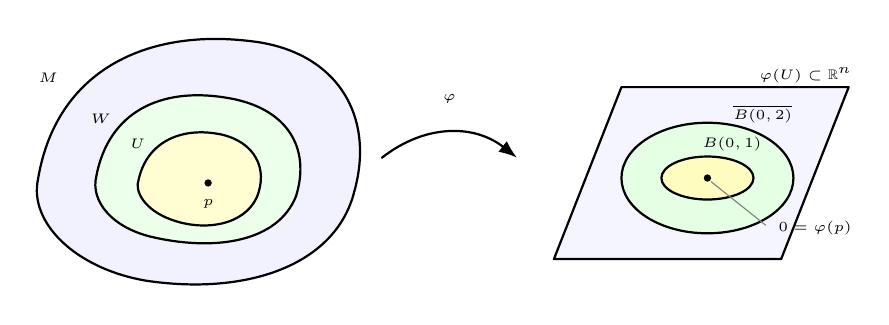
\begin{tikzpicture}[
    >=Latex,
    font=\small,
    line cap=round,
    line join=round,
    scale=0.78
]

% M
\draw[
    thick,
    fill=blue!5
]
    (-5.4,0.1)
    .. controls (-5.1,1.9) and (-3.6,2.55) .. (-1.95,2.35)
    .. controls (-0.55,2.2) and (0.10,1.15) .. (-0.25,-0.10)
    .. controls (-0.55,-1.30) and (-2.0,-1.80) .. (-3.65,-1.55)
    .. controls (-4.8,-1.35) and (-5.55,-0.60) .. (-5.4,0.1);

\node[anchor=west, font=\tiny] at (-5.55,1.75)
    {$M$};

% W
\draw[
    thick,
    fill=green!8
]
    (-4.45,0.15)
    .. controls (-4.25,1.20) and (-3.40,1.60) .. (-2.35,1.43)
    .. controls (-1.35,1.28) and (-0.95,0.62) .. (-1.20,-0.18)
    .. controls (-1.50,-0.92) and (-2.50,-1.07) .. (-3.50,-0.85)
    .. controls (-4.20,-0.70) and (-4.55,-0.25) .. (-4.45,0.15);

\node[anchor=west, font=\tiny] at (-4.70,1.08)
    {$W$};

% U
\draw[
    thick,
    fill=yellow!18
]
    (-3.76,0.10)
    .. controls (-3.62,0.72) and (-3.05,0.96) .. (-2.42,0.83)
    .. controls (-1.88,0.71) and (-1.64,0.28) .. (-1.84,-0.20)
    .. controls (-2.05,-0.65) and (-2.70,-0.76) .. (-3.25,-0.55)
    .. controls (-3.65,-0.40) and (-3.84,-0.10) .. (-3.76,0.10);

\node[anchor=west, font=\tiny] at (-4.05,0.67)
    {$U$};

% Punkt p
\fill (-2.63,0.04) circle (1.7pt);

\node[below=5pt, font=\tiny] at (-2.63,0.15)
    {$p$};

% Strzałka \varphi
\draw[->,thick]
    (0.20,0.45)
    .. controls (0.90,1.00) and (1.70,1.00) ..
    (2.40,0.45);

\node[above=5pt, font=\tiny] at (1.30,0.95)
    {$\varphi$};

% Obraz mapy
\draw[
    thick,
    fill=blue!4
]
    (3.0,-1.2)
    --
    (4.1,1.6)
    --
    (7.8,1.6)
    --
    (6.7,-1.2)
    --
    cycle;

\node[above=7pt, font=\tiny] at (7.10,1.20)
    {$\varphi(U)\subset\mathbb{R}^n$};

% \overline{B(0,2)}
\draw[
    thick,
    fill=green!10
]
    (5.50,0.12)
    ellipse (1.40 and 0.9);

\node[above=8pt, font=\tiny] at (6.40,0.5)
    {$\overline{B(0,2)}$};

% B(0,1)
\draw[
    thick,
    fill=yellow!25
]
    (5.50,0.12)
    ellipse (0.75 and 0.35);

\node[below=7pt, font=\tiny] at (5.90, 1.26)
    {$B(0,1)$};

% 0 = \varphi(p)
\fill (5.50,0.12) circle (1.7pt);

\draw[thin,gray] (5.56,0.06) -- (6.45,-0.65);
\node[anchor=west, font=\tiny] at (6.50,-0.70)
    {$0=\varphi(p)$};

\end{tikzpicture}

\caption{
Wybór mapy $(U,\varphi)$ wokół punktu $p$:
$U\subseteq W$, $\varphi(p)=0$ oraz
$\overline{B(0,2)}\subseteq\varphi(U)$.
}
\label{fig:kapelusz-mapa}

\end{figure}


% ============================================================
% RYSUNEK 2
% Wykres funkcji kapelusz
% ============================================================

\begin{figure}[ht]
\centering

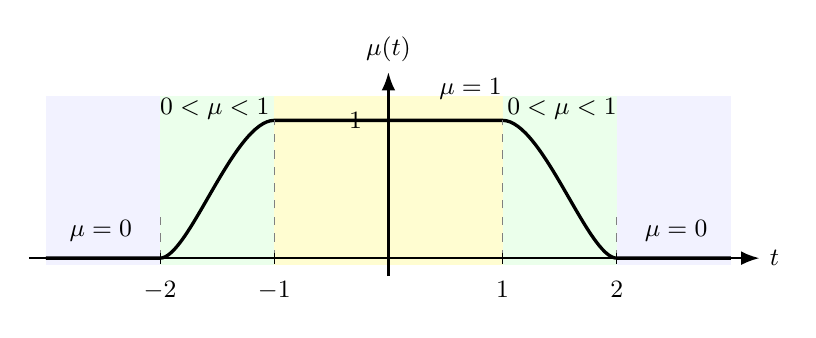
\begin{tikzpicture}[
    >=Latex,
    font=\small,
    x=1.45cm,
    y=1.75cm
]

% Delikatne kolorowe obszary
\fill[blue!5]
    (-3,-0.05)
    rectangle
    (-2,1.18);

\fill[green!8]
    (-2,-0.05)
    rectangle
    (-1,1.18);

\fill[yellow!18]
    (-1,-0.05)
    rectangle
    (1,1.18);

\fill[green!8]
    (1,-0.05)
    rectangle
    (2,1.18);

\fill[blue!5]
    (2,-0.05)
    rectangle
    (3,1.18);

% Oś pozioma
\draw[->,thick]
    (-3.15,0)
    --
    (3.25,0)
    node[right] {$t$};

% Oś pionowa
\draw[->,thick]
    (0,-0.13)
    --
    (0,1.35)
    node[above] {$\mu(t)$};

% Wykres funkcji kapelusz
\draw[very thick]
    (-3,0)
    --
    (-2,0)
    .. controls (-1.75,0) and (-1.35,1) ..
    (-1,1)
    --
    (1,1)
    .. controls (1.35,1) and (1.75,0) ..
    (2,0)
    --
    (3,0);

% Linie pomocnicze
\draw[dashed,gray]
    (-1,0) -- (-1,1);

\draw[dashed,gray]
    (1,0) -- (1,1);

\draw[dashed,gray]
    (-2,0) -- (-2,0.36);

\draw[dashed,gray]
    (2,0) -- (2,0.36);

% Znaczniki na osi
\draw
    (-2,0.04) -- (-2,-0.04);
\node[below=5pt] at (-2,0)
    {$-2$};

\draw
    (-1,0.04) -- (-1,-0.04);
\node[below=5pt] at (-1,0)
    {$-1$};

\draw
    (1,0.04) -- (1,-0.04);
\node[below=5pt] at (1,0)
    {$1$};

\draw
    (2,0.04) -- (2,-0.04);
\node[below=5pt] at (2,0)
    {$2$};

% Poziom 1
\draw
    (-0.04,1) -- (0.04,1);

\node[left=6pt] at (0,1)
    {$1$};

% Opisy — odsunięte od wykresu
\node[above=4pt] at (0.72,1)
    {$\mu=1$};

\node at (-1.52,1.08)
    {$0<\mu<1$};

\node at (1.52,1.08)
    {$0<\mu<1$};

\node at (-2.52,0.20)
    {$\mu=0$};

\node at (2.52,0.20)
    {$\mu=0$};

\end{tikzpicture}

\caption{
Jednowymiarowy przekrój funkcji odcinającej $\mu$.
Funkcja jest równa $1$ dla $|t|\leq1$,
płynnie maleje dla $1<|t|<2$
i znika dla $|t|\geq2$.
}
\label{fig:kapelusz-wykres}

\end{figure}




\begin{lemat}[Lokalność derywacji]\label{lem:lokalnosc}
Niech $v\in T_p^CM$ będzie derywacją w $p$. Jeśli $h\in C^\infty(M)$ znika na pewnym
otoczeniu punktu $p$, to $v(h)=0$. W szczególności, jeśli $f,g\in C^\infty(M)$ pokrywają
się na pewnym otoczeniu $p$, to $v(f)=v(g)$; wartość $v(f)$ zależy więc jedynie od
zachowania $f$ w dowolnie małym otoczeniu $p$.
\end{lemat}
\begin{proof}
Z reguły Leibniza zastosowanej do $f=g=\mathbf1$ (funkcji stałej równej $1$),
$v(\mathbf1)=v(\mathbf1\cdot\mathbf1)=2v(\mathbf1)$, skąd $v(\mathbf1)=0$; z liniowości,
$v(c)=0$ dla każdej funkcji stałej $c$.

Niech $h\equiv0$ na otoczeniu otwartym $W\ni p$. Wybierzmy mapę $(U,\varphi)$ wokół $p$ z
$U\subseteq W$, $\varphi(p)=0$, oraz (po przeskalowaniu)
$\overline{B(0,2)}\subseteq\varphi(U)$.
Zdefiniujmy $\tilde\mu\colon M\to\R$: $\tilde\mu(q):=\mu(\varphi(q))$ dla $q\in U$, oraz
$\tilde\mu(q):=0$ dla $q\notin U$. Nośnik jest zawarty w zwartym
zbiorze $K=\varphi^{-1}(\overline{B(0,2)})\subset U$.
Ponieważ $M$ jest Hausdorffa, $K$ jest domknięty w $M$.
Na otwartym pokryciu $U, M\setminus K$ obie gładkie definicje
pokrywają się, więc $\tilde\mu\in C^\infty(M)$, równa $1$ na otoczeniu $p$ i znikająca poza
$U\subseteq W$. Wówczas $\tilde\mu\cdot h\equiv0$ na całym $M$, więc $v(\tilde\mu h)=0$.
Z reguły Leibniza, $0=v(\tilde\mu h)=\tilde\mu(p)v(h)+h(p)v(\tilde\mu)=v(h)$ (bo
$\tilde\mu(p)=1$, $h(p)=0$). Zatem $v(h)=0$. Ostatnia część lematu wynika z zastosowania
powyższego do $h:=f-g$.
\end{proof}

\begin{twierdzenie}\label{tw:baza-styczna}
Niech $(U,\varphi)$ będzie mapą dopuszczalną wokół $p$,
$\varphi=(x^1,\dots,x^n)$,
gdzie $x^i=\pi_i\circ\varphi\colon U\to\R$ są funkcjami współrzędnymi,
czyli dla każdego $q\in U$ zachodzi
$\varphi(q)=\bigl(x^1(q),\dots,x^n(q)\bigr)$,
oraz załóżmy, że $\varphi(p)=0$. Wówczas:
\begin{enumerate}[label=(\alph*)]
\item Odwzorowanie $\Phi\colon T_p^AM\to T_p^CM$ jest izomorfizmem liniowym.
\item Elementy $\frac{\partial}{\partial x^1}\big|_p,\dots,\frac{\partial}{\partial x^n}
\big|_p\in T_p^CM$, zdefiniowane przez $\frac{\partial}{\partial x^i}\big|_p(f):=
\frac{\partial(f\circ\varphi^{-1})}{\partial x^i}(\varphi(p))$, stanowią bazę $T_p^CM$.
W szczególności $\dim T_pM=n$.
\end{enumerate}
\end{twierdzenie}

\begin{proof}
\emph{(a), injektywność.} Załóżmy $\Phi([\gamma])=0$, tzn.\ $(f\circ\gamma)'(0)=0$ dla
wszystkich $f\in C^\infty(M)$. Wybierzmy funkcję odcinającą
$\tilde\mu$ o zwartym nośniku zawartym w $U$, równą $1$ blisko $p$,
jak w dowodzie Lematu~\ref{lem:lokalnosc}.
Dla $i=1,\dots,n$ niech $\tilde x^i:=\tilde\mu\,x^i
=\tilde\mu\,\varphi^i$ na $U$ (rozszerzone przez $0$ poza $U$) —
funkcja gładka na $M$, pokrywająca się z $\varphi^i$ na otoczeniu $p$. Z założenia,
$0=\Phi([\gamma])(\tilde x^i)=(\tilde x^i\circ\gamma)'(0)$; blisko $t=0$, $\gamma(t)\in U$
i tam $\tilde x^i\circ\gamma=\varphi^i\circ\gamma$, więc $(\varphi^i\circ\gamma)'(0)=0$ dla
każdego $i$, czyli $(\varphi\circ\gamma)'(0)=0\in\R^n$. Oznacza to $\gamma\sim
\gamma_{\text{stała}}$ (gdzie $\gamma_{\text{stała}}(t)\equiv p$), czyli $[\gamma]=0$ w
$T_p^AM$. Zatem $\ker\Phi=\{0\}$.

\emph{(a), surjektywność — Lemat Hadamarda.} Niech $v\in T_p^CM$. Bez straty ogólności
$\varphi(U)$ jest kulą (gwiaździstą względem $0$). Niech $\tilde f:=f\circ\varphi^{-1}\in
C^\infty(\varphi(U))$; z Lematu~\ref{lem:hadamard} istnieją $g_1,\dots,g_n$ z
\[
\tilde f(x)=\tilde f(0)+\sum_ix^ig_i(x), \qquad g_i(0)=\frac{\partial\tilde f}{\partial x^i}
(0)=\frac{\partial}{\partial x^i}\Big|_p(f).
\]
Podstawiając $x=\varphi(q)$: $f(q)=f(p)+\sum_i\varphi^i(q)\,g_i(\varphi(q))$ dla $q$
blisko $p$. Niech $\widetilde{\varphi^i}$, $\tilde g_i$ oznaczają (jak wyżej) rozszerzenia
$\varphi^i$ oraz $g_i\circ\varphi$ do funkcji gładkich na $M$, pokrywające się z
oryginałami na otoczeniu $p$. Funkcja $F:=f(p)\cdot\mathbf1+\sum_i\widetilde{\varphi^i}\,
\tilde g_i$ pokrywa się z $f$ na otoczeniu $p$, więc $v(f)=v(F)$ (Lemat~\ref{lem:lokalnosc}).
Z liniowości $v$, reguły Leibniza (korzystając z $\widetilde{\varphi^i}(p)=0$,
$v(\mathbf1)=0$):
\[
v(f)=v(F)=\sum_i\Big(\widetilde{\varphi^i}(p)\,v(\tilde g_i)+\tilde g_i(p)\,v
(\widetilde{\varphi^i})\Big)=\sum_ig_i(0)\,v(\widetilde{\varphi^i})=\sum_{i=1}^n
v(\widetilde{\varphi^i})\cdot\frac{\partial}{\partial x^i}\Big|_p(f).
\]
Kładąc $c_i:=v(\widetilde{\varphi^i})\in\R$, mamy $v=\sum_ic_i\,\frac{\partial}{\partial
x^i}\big|_p$ jako funkcjonały. Niech $\gamma(t):=\varphi^{-1}(t\cdot(c_1,\dots,c_n))$; wtedy
$\Phi([\gamma])(f)=(f\circ\gamma)'(0)=D(f\circ\varphi^{-1})(0)\cdot(c_1,\dots,c_n)=
\sum_ic_i\frac{\partial}{\partial x^i}\big|_p(f)=v(f)$ dla każdego $f$, czyli
$\Phi([\gamma])=v$. To dowodzi surjektywności, a wraz z liniowością i injektywnością —
części (a).

\emph{(b).} Powyższy rachunek pokazał, że każdy $v\in T_p^CM$ jest kombinacją liniową
$\sum_ic_i\frac{\partial}{\partial x^i}\big|_p$ — więc baza ta rozpina $T_p^CM$. Niezależność
liniowa: załóżmy $\sum_ic_i\frac{\partial}{\partial x^i}\big|_p=0$. Stosując obie strony
do $\widetilde{\varphi^j}$ i korzystając z $\frac{\partial}{\partial x^i}\big|_p
(\widetilde{\varphi^j})=\frac{\partial x^j}{\partial x^i}(0)=\delta_i^j$, otrzymujemy
$0=\sum_ic_i\delta_i^j=c_j$ dla każdego $j$. Zatem $\{\partial/\partial x^i|_p\}$ jest
bazą $T_p^CM$; w szczególności $\dim T_p^CM=n$.
\end{proof}

\begin{wniosek}
Definicje A, B i C przestrzeni stycznej są kanonicznie izomorficzne. Piszemy odtąd po
prostu $T_pM$ i mówimy o \emph{przestrzeni stycznej do $M$ w punkcie $p$} — jest to
$n$-wymiarowa przestrzeń wektorowa. W mapie $(U,\varphi)$, gdzie $\varphi=(x^1,\dots,x^n)$,
jej \emph{bazą współrzędnościową} są wektory
\[
\left.\frac{\partial}{\partial x^1}\right|_p,\ \dots,\
\left.\frac{\partial}{\partial x^n}\right|_p.
\]
\end{wniosek}

\begin{figure}[ht]
\centering
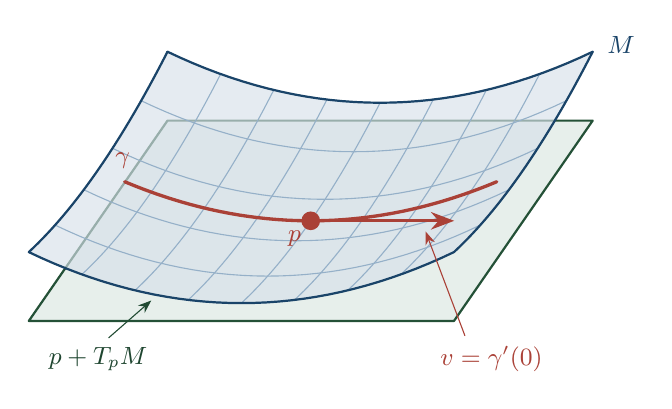
\begin{tikzpicture}[>=Stealth,scale=1.35,line cap=round,line join=round]
% S(u,v)=(u,v,.12u^2+.08v^2), rzut (x,y,z)->(x+.45y,.65y+z).
% Brzeg wypełnienia, siatka i krzywa używają tej samej parametryzacji.
\filldraw[fill=manifoldgreen!12,draw=manifoldgreen!65!black,thick]
 (-2.6525,-.9425)--(1.3475,-.9425)--(2.6525,.9425)--(-1.3475,.9425)--cycle;
\path[fill=manifoldblue!18,opacity=.65]
 (-2.65250,-0.29430)
  --(-2.48583,-0.37097)
  --(-2.31917,-0.44097)
  --(-2.15250,-0.50430)
  --(-1.98583,-0.56097)
  --(-1.81917,-0.61097)
  --(-1.65250,-0.65430)
  --(-1.48583,-0.69097)
  --(-1.31917,-0.72097)
  --(-1.15250,-0.74430)
  --(-0.98583,-0.76097)
  --(-0.81917,-0.77097)
  --(-0.65250,-0.77430)
  --(-0.48583,-0.77097)
  --(-0.31917,-0.76097)
  --(-0.15250,-0.74430)
  --(0.01417,-0.72097)
  --(0.18083,-0.69097)
  --(0.34750,-0.65430)
  --(0.51417,-0.61097)
  --(0.68083,-0.56097)
  --(0.84750,-0.50430)
  --(1.01417,-0.44097)
  --(1.18083,-0.37097)
  --(1.34750,-0.29430)
  --(1.40187,-0.24262)
  --(1.45625,-0.18861)
  --(1.51063,-0.13226)
  --(1.56500,-0.07358)
  --(1.61938,-0.01256)
  --(1.67375,0.05080)
  --(1.72812,0.11649)
  --(1.78250,0.18452)
  --(1.83688,0.25489)
  --(1.89125,0.32759)
  --(1.94562,0.40263)
  --(2.00000,0.48000)
  --(2.05437,0.55971)
  --(2.10875,0.64176)
  --(2.16312,0.72614)
  --(2.21750,0.81286)
  --(2.27188,0.90191)
  --(2.32625,0.99330)
  --(2.38063,1.08703)
  --(2.43500,1.18309)
  --(2.48937,1.28149)
  --(2.54375,1.38222)
  --(2.59813,1.48529)
  --(2.65250,1.59070)
  --(2.48583,1.51403)
  --(2.31917,1.44403)
  --(2.15250,1.38070)
  --(1.98583,1.32403)
  --(1.81917,1.27403)
  --(1.65250,1.23070)
  --(1.48583,1.19403)
  --(1.31917,1.16403)
  --(1.15250,1.14070)
  --(0.98583,1.12403)
  --(0.81917,1.11403)
  --(0.65250,1.11070)
  --(0.48583,1.11403)
  --(0.31917,1.12403)
  --(0.15250,1.14070)
  --(-0.01417,1.16403)
  --(-0.18083,1.19403)
  --(-0.34750,1.23070)
  --(-0.51417,1.27403)
  --(-0.68083,1.32403)
  --(-0.84750,1.38070)
  --(-1.01417,1.44403)
  --(-1.18083,1.51403)
  --(-1.34750,1.59070)
  --(-1.40187,1.48529)
  --(-1.45625,1.38222)
  --(-1.51063,1.28149)
  --(-1.56500,1.18309)
  --(-1.61938,1.08703)
  --(-1.67375,0.99330)
  --(-1.72812,0.90191)
  --(-1.78250,0.81286)
  --(-1.83688,0.72614)
  --(-1.89125,0.64176)
  --(-1.94562,0.55971)
  --(-2.00000,0.48000)
  --(-2.05437,0.40263)
  --(-2.10875,0.32759)
  --(-2.16312,0.25489)
  --(-2.21750,0.18452)
  --(-2.27188,0.11649)
  --(-2.32625,0.05080)
  --(-2.38063,-0.01256)
  --(-2.43500,-0.07358)
  --(-2.48937,-0.13226)
  --(-2.54375,-0.18861)
  --(-2.59813,-0.24262) --cycle;
\foreach \vv in {-1.45,-.9,-.3,.3,.9,1.45}{
 \draw[manifoldblue!48,thin] plot[domain=-2:2,samples=35]
  ({\x+.45*\vv},{.65*\vv+.12*\x*\x+.08*\vv*\vv});}
\foreach \uu in {-2,-1.5,-1,-.5,0,.5,1,1.5,2}{
 \draw[manifoldblue!48,thin] plot[domain=-1.45:1.45,samples=30]
  ({\uu+.45*\x},{.65*\x+.12*\uu*\uu+.08*\x*\x});}
\foreach \vv in {-1.45,1.45}{
 \draw[manifoldblue!75!black,thick] plot[domain=-2:2,samples=35]
  ({\x+.45*\vv},{.65*\vv+.12*\x*\x+.08*\vv*\vv});}
\foreach \uu in {-2,2}{
 \draw[manifoldblue!75!black,thick] plot[domain=-1.45:1.45,samples=30]
  ({\uu+.45*\x},{.65*\x+.12*\uu*\uu+.08*\x*\x});}
\draw[manifoldred,very thick] plot[domain=-1.75:1.75,samples=40]
 ({\x},{.12*\x*\x});
\fill[manifoldred] (0,0) circle (2.5pt) node[below left,font=\small] {$p$};
\draw[->,very thick,manifoldred] (0,0)--(1.35,0);
\node[font=\small,manifoldred] at (-1.77,.57) {$\gamma$};
\node[font=\small\bfseries,manifoldblue!75!black] at (2.92,1.65) {$M$};
\node[font=\small,manifoldgreen!55!black] at (-2.0,-1.30) {$p+T_pM$};
\draw[->,manifoldgreen!60!black,thin] (-1.9,-1.10)--(-1.5,-.75);
\node[font=\small,manifoldred] at (1.7,-1.30) {$v=\gamma'(0)$};
\draw[->,manifoldred,thin] (1.45,-1.08)--(1.08,-.10);
\end{tikzpicture}
\caption{Przestrzeń styczna: zielony równoległobok przedstawia afiniczną
płaszczyznę $p+T_pM$ przy zanurzonej powierzchni $M$. Czerwona krzywa
$\gamma$ leży na $M$, a wektor $v=\gamma'(0)$ leży w płaszczyźnie stycznej.
Siatka powierzchni odchyla się od tej płaszczyzny poza punktem $p$.}
\label{fig:tangent}
\end{figure}


\subsection*{Zmiana współrzędnych wektora stycznego}

\begin{fakt}
Niech $(U,\varphi)$ i $(V,\psi)$ będą mapami wokół $p\in M$, a
$[\gamma]\in T_pM$, gdzie $\gamma:(-\varepsilon,\varepsilon)\to M, \ \gamma(0)=p$.
Współrzędne wektora $[\gamma]$ w mapie $\varphi$ są dane przez $[\gamma]_{\varphi}:=(\varphi\circ\gamma)'(0)\in\R^n$,
a w mapie $\psi$ przez $[\gamma]_{\psi}:=(\psi\circ\gamma)'(0)$.
Wtedy
\[
\boxed{
[\gamma]_{\psi}
=
D(\psi\circ\varphi^{-1})(\varphi(p))\,[\gamma]_{\varphi}.
}
\]
\end{fakt}

\begin{proof}
Ponieważ $\psi\circ\gamma = (\psi\circ\varphi^{-1})\circ(\varphi\circ\gamma)$,
z reguły łańcuchowej otrzymujemy
\[
(\psi\circ\gamma)'(0)
=
D(\psi\circ\varphi^{-1})(\varphi(p))
\,(\varphi\circ\gamma)'(0),
\]
czyli dokładnie
\[
[\gamma]_{\psi}
=
D(\psi\circ\varphi^{-1})(\varphi(p))\,[\gamma]_{\varphi}.
\]
\end{proof}
Jak pokaże następna sekcja, jedną z najbardziej użytecznych definicji
przestrzeni stycznej jest konstrukcja za pomocą derywacji.
Podamy zatem regułę transformacji wektorów stycznych również
w tym ujęciu.

\begin{fakt}[Transformacja derywacji współrzędnych]
\label{fakt:transformacja-derywacji}
Niech $(U,\varphi)$ i $(V,\psi)$ będą mapami rozmaitości
$M$ wokół punktu $p\in U\cap V$, przy czym $\varphi=(x^1,\ldots,x^n), \ \psi=(y^1,\ldots,y^n)$.
Niech
\[
\left\{
\left.\frac{\partial}{\partial x^i}\right|_p
\right\}_{i=1}^n,
\qquad
\left\{
\left.\frac{\partial}{\partial y^j}\right|_p
\right\}_{j=1}^n
\]
oznaczają odpowiadające tym mapom bazy przestrzeni
stycznej $T_pM$, zdefiniowane za pomocą derywacji.

Wówczas zachodzi \emph{reguła transformacji derywacji
współrzędnych}:
\begin{equation}
\label{eq:transformacja-derywacji}
\boxed{
\left.\frac{\partial}{\partial x^i}\right|_p
=
\sum_{j=1}^n
\frac{\partial y^j}{\partial x^i}(p)
\left.\frac{\partial}{\partial y^j}\right|_p,
\qquad i=1,\ldots,n,
}
\end{equation}
gdzie
\[
\frac{\partial y^j}{\partial x^i}(p)
:=
\left.
\frac{\partial(y^j\circ\varphi^{-1})}{\partial u^i}
\right|_{u=\varphi(p)},
\]
a $u^1,\ldots,u^n$ oznaczają standardowe współrzędne
w $\R^n$.

Współczynniki te są elementami macierzy Jacobiego
odwzorowania przejścia:
\[
\boxed{
J_{\psi\varphi}(p)
:=
D(\psi\circ\varphi^{-1})(\varphi(p))
=
\left[
\frac{\partial y^j}{\partial x^i}(p)
\right]_{j,i=1}^n.
}
\]
\end{fakt}

\begin{proof}
Przypomnijmy, że dla dowolnej funkcji $f$ gładkiej
w otoczeniu punktu $p$ derywacje współrzędnych
są określone wzorami
\[
\left.\frac{\partial}{\partial x^i}\right|_p(f)
=
\left.
\frac{\partial(f\circ\varphi^{-1})}{\partial u^i}
\right|_{u=\varphi(p)}
\]
oraz
\[
\left.\frac{\partial}{\partial y^j}\right|_p(f)
=
\left.
\frac{\partial(f\circ\psi^{-1})}{\partial v^j}
\right|_{v=\psi(p)},
\]
gdzie $u^i$ i $v^j$ są standardowymi współrzędnymi
w $\R^n$.

Rozważmy odwzorowanie przejścia
\[
F:=\psi\circ\varphi^{-1}
\colon
\varphi(U\cap V)\longrightarrow\psi(U\cap V).
\]
Ponieważ $\psi=(y^1,\ldots,y^n)$,
jego funkcje współrzędne mają postać $F^j=y^j\circ\varphi^{-1}, \ j=1,\ldots,n$.
W szczególności, przy oznaczeniach $u:=\varphi(p), \ v:=\psi(p)=F(u)$,
otrzymujemy
\[
DF(u)
=
\left[
\frac{\partial F^j}{\partial u^i}(u)
\right]_{j,i=1}^n
=
\left[
\frac{\partial y^j}{\partial x^i}(p)
\right]_{j,i=1}^n
=
J_{\psi\varphi}(p).
\]

Zauważmy teraz, że w otoczeniu punktu $u$
możemy wstawić identyczność
$\psi^{-1}\circ\psi$ i zapisać
\[
f\circ\varphi^{-1}
=f\circ\psi^{-1}\circ\psi\circ\varphi^{-1}
=(f\circ\psi^{-1})\circ(\psi\circ\varphi^{-1})
=(f\circ\psi^{-1})\circ F.
\]

Stosując regułę łańcuchową, otrzymujemy
\[
\boxed{
D(f\circ\varphi^{-1})(u)
=
D(f\circ\psi^{-1})(v)\,DF(u).
}
\]

Rozpiszmy tę równość w postaci macierzowej:
\[
\begin{gathered}
\underbrace{
\begin{pmatrix}
\displaystyle
\frac{\partial(f\circ\varphi^{-1})}{\partial u^1}(u)
&
\cdots
&
\displaystyle
\frac{\partial(f\circ\varphi^{-1})}{\partial u^n}(u)
\end{pmatrix}
}_{1\times n}
\\[1mm]
=
\underbrace{
\begin{pmatrix}
\displaystyle
\frac{\partial(f\circ\psi^{-1})}{\partial v^1}(v)
&
\cdots
&
\displaystyle
\frac{\partial(f\circ\psi^{-1})}{\partial v^n}(v)
\end{pmatrix}
}_{1\times n}
\underbrace{
\begin{pmatrix}
\displaystyle\frac{\partial y^1}{\partial x^1}
&\cdots&
\displaystyle\frac{\partial y^1}{\partial x^n}
\\[2mm]
\vdots&\ddots&\vdots
\\[2mm]
\displaystyle\frac{\partial y^n}{\partial x^1}
&\cdots&
\displaystyle\frac{\partial y^n}{\partial x^n}
\end{pmatrix}_{\!p}
}_{n\times n}.
\end{gathered}
\]

Korzystając z definicji derywacji współrzędnych,
możemy tę samą równość zapisać krócej:
\[
\begin{pmatrix}
\displaystyle
\left.\frac{\partial}{\partial x^1}\right|_p(f)
&
\cdots
&
\displaystyle
\left.\frac{\partial}{\partial x^n}\right|_p(f)
\end{pmatrix}
=
\begin{pmatrix}
\displaystyle
\left.\frac{\partial}{\partial y^1}\right|_p(f)
&
\cdots
&
\displaystyle
\left.\frac{\partial}{\partial y^n}\right|_p(f)
\end{pmatrix}
J_{\psi\varphi}(p).
\]

Porównując $i$-te współrzędne obu stron,
dostajemy
\[
\left.\frac{\partial}{\partial x^i}\right|_p(f)
=
\sum_{j=1}^n
\frac{\partial y^j}{\partial x^i}(p)
\left.\frac{\partial}{\partial y^j}\right|_p(f).
\]

Ponieważ równość ta zachodzi dla każdej funkcji
$f$ gładkiej w otoczeniu $p$, obie strony
wyznaczają tę samą derywację w punkcie $p$.
Otrzymujemy zatem wzór
\eqref{eq:transformacja-derywacji}.
\end{proof}

Zauważmy, że macierz Jacobiego $J_{\psi\varphi}(p) = D(\psi\circ\varphi^{-1})(\varphi(p))$
jest dokładnie macierzą współczynników występujących
w regule transformacji derywacji
\eqref{eq:transformacja-derywacji}.
W zapisie macierzowym reguła ta przyjmuje postać
\[
\boxed{
\begin{pmatrix}
\displaystyle\left.\frac{\partial}{\partial x^1}\right|_p
&
\cdots
&
\displaystyle\left.\frac{\partial}{\partial x^n}\right|_p
\end{pmatrix}
=
\begin{pmatrix}
\displaystyle\left.\frac{\partial}{\partial y^1}\right|_p
&
\cdots
&
\displaystyle\left.\frac{\partial}{\partial y^n}\right|_p
\end{pmatrix}
J_{\psi\varphi}(p).
}
\]

W szczególności, jeżeli wektor styczny $X\in T_pM$
ma w obu bazach przedstawienia
\[
X=
\sum_{i=1}^n X_\varphi^i
\left.\frac{\partial}{\partial x^i}\right|_p
=
\sum_{j=1}^n X_\psi^j
\left.\frac{\partial}{\partial y^j}\right|_p,
\]
to jego kolumny współrzędnych spełniają
\[
\boxed{
\begin{pmatrix}
X_\psi^1\\
\vdots\\
X_\psi^n
\end{pmatrix}
=
D(\psi\circ\varphi^{-1})(\varphi(p))
\begin{pmatrix}
X_\varphi^1\\
\vdots\\
X_\varphi^n
\end{pmatrix}.
}
\]

Zatem różniczka odwzorowania przejścia
$\psi\circ\varphi^{-1}$ opisuje zarówno
transformację baz przestrzeni stycznej,
jak i transformację współrzędnych wektorów stycznych.

\begin{przyklad}[Zmiana współrzędnych wektora stycznego na $\mathbb{RP}^2$]
\label{prz:RP2-styczna-1}
Wróćmy do map z przykładu~\ref{prz:RP2-przejscie-1}:
punkt $[1:u:v]$, gdzie $u\ne0$, ma w drugiej mapie współrzędne
$(a,b)=(1/u,v/u)$. Zastosujemy do tego przejścia właśnie udowodnioną
regułę zmiany współrzędnych wektora stycznego.

Odwzorowanie $\varphi_1\circ\varphi_0^{-1}$ opisuje zmianę
\emph{współrzędnych punktów} rozmaitości. Jego różniczka opisuje natomiast
odpowiadającą jej zmianę \emph{współrzędnych wektorów stycznych}.

Niech $p\in U_0\cap U_1$ oraz $\varphi_0(p)=(u,v)$.
Mapy $\varphi_0$ i $\varphi_1$ wyznaczają dwie bazy przestrzeni stycznej
$T_p\mathbb{RP}^2$:
\[
\left\{
\left.\frac{\partial}{\partial u}\right|_p,
\left.\frac{\partial}{\partial v}\right|_p
\right\},
\qquad
\left\{
\left.\frac{\partial}{\partial a}\right|_p,
\left.\frac{\partial}{\partial b}\right|_p
\right\}.
\]
Jeżeli wektor $X\in T_p\mathbb{RP}^2$ ma w bazie indukowanej przez
$\varphi_0$ współrzędne
\[
X
=
\dot u\left.\frac{\partial}{\partial u}\right|_p
+
\dot v\left.\frac{\partial}{\partial v}\right|_p,
\]
to jego współrzędne w bazie indukowanej przez $\varphi_1$ otrzymujemy,
stosując różniczkę odwzorowania przejścia:
\[
\begin{pmatrix}
\dot a\\[1mm]
\dot b
\end{pmatrix}
=
D(\varphi_1\circ\varphi_0^{-1})(u,v)
\begin{pmatrix}
\dot u\\[1mm]
\dot v
\end{pmatrix}.
\]
A zatem
\[
\dot a=-\frac{\dot u}{u^2},
\qquad
\dot b
=
-\frac{v\dot u}{u^2}
+
\frac{\dot v}{u}.
\]
Ten sam wektor styczny możemy więc zapisać jako
\[
X
=
\dot u\left.\frac{\partial}{\partial u}\right|_p
+
\dot v\left.\frac{\partial}{\partial v}\right|_p
=
\dot a\left.\frac{\partial}{\partial a}\right|_p
+
\dot b\left.\frac{\partial}{\partial b}\right|_p.
\]

Innymi słowy, odwzorowanie przejścia
$\varphi_1\circ\varphi_0^{-1}$ zmienia współrzędne punktu na rozmaitości,
natomiast jego różniczka $d(\varphi_1\circ\varphi_0^{-1})_{\varphi_0(p)}$
zmienia reprezentację współrzędnościową tego samego wektora
$X\in T_p\mathbb{RP}^2$ względem baz przestrzeni stycznej indukowanych
przez obie mapy.
\end{przyklad}

\subsection*{Przestrzeń styczna w punkcie brzegu}

Niech teraz $p\in\partial M$. \emph{Kiełek}\index{kielek funkcji@Kiełek funkcji} funkcji gładkiej w $p$
to jej klasa względem równości w pewnym otoczeniu punktu $p$
otwartym w $M$;
funkcje są tu gładkie w sensie przedłużalności z półprzestrzeni.
Ich algebra to $C^\infty_p(M)$. Definiujemy $T_pM$ jako przestrzeń
$\R$-liniowych derywacji $D:C^\infty_p(M)\to\R$ spełniających $D(fg)=f(p)D(g)+g(p)D(f)$.
Wartość kiełka w $p$ jest dobrze określona. To lokalna wersja
Definicji C, która nie wymaga krzywej przechodzącej przez $p$
w obu kierunkach czasu.

Użycie kiełków jest tutaj istotne. Gładkie przedłużenie funkcji
$f$ poza brzeg, do otoczenia $\varphi(p)$ w $\R^n$, nie jest
jednoznaczne i stanowi jedynie pomocnicze narzędzie służące do
zdefiniowania gładkości. Przestrzeń styczna powinna natomiast zależeć
wyłącznie od lokalnego zachowania funkcji na samej rozmaitości $M$,
a nie od arbitralnego wyboru jej wartości poza $M$.

Dokładniej, dwa różne gładkie przedłużenia
$\widetilde f_1,\widetilde f_2$ mogą być różnymi funkcjami na
otoczeniu $\varphi(p)$ w $\R^n$, mimo że ich ograniczenia do
$\mathbb H^n$ wyznaczają tę samą funkcję na $M$. Nie chcemy więc
traktować samych przedłużeń jako obiektów, na których działa derywacja.
Obiektem właściwym jest kiełek funkcji na $M$, natomiast przedłużenie
wybieramy dopiero wtedy, gdy chcemy wykonać rachunek we współrzędnych.

Co więcej, derywacja w punkcie $p$ jest obiektem lokalnym: jej wartość
na funkcji zależy jedynie od zachowania tej funkcji w dowolnie małym
otoczeniu $p$. Dlatego naturalną dziedziną derywacji jest algebra
kiełków $C^\infty_p(M)$.

\begin{stwierdzenie}[Pełny wymiar przestrzeni stycznej przy brzegu]
\label{prop:styczna-brzeg-1}
W mapie półprzestrzennej $\varphi$ z $\varphi(p)=0$ każda taka
derywacja ma jednoznaczną postać
\[
D(f)=\sum_{i=1}^n v^i\partial_i\widetilde f(0),
\qquad v\in\R^n,
\]
gdzie $\widetilde f$ jest dowolnym gładkim przedłużeniem
$f\circ\varphi^{-1}$ na otoczenie zera w $\R^n$.
Wzór nie zależy od wyboru przedłużenia. Przy zmianie mapy współrzędne
$v$ zmieniają się przez odwracalną macierz Jacobiego przejścia.
W szczególności $\dim T_pM=n$, a inkluzja brzegu identyfikuje
$T_p\partial M$ z podprzestrzenią $v^n=0$.
\end{stwierdzenie}

\begin{proof}
Najpierw sprawdźmy, że prawa strona wzoru nie zależy od wyboru
przedłużenia $\widetilde f$. Jeżeli $\widetilde f_1$ i
$\widetilde f_2$ są dwoma gładkimi przedłużeniami reprezentującymi
ten sam kiełek funkcji $f\circ\varphi^{-1}$, to ich różnica znika
na pewnej małej półkuli $B_\varepsilon(0)\cap\mathbb H^n$.
Na jej części wewnętrznej, gdzie $x^n>0$, znikają więc wszystkie
pierwsze pochodne tej różnicy, a przez ciągłość znikają one również
w punkcie $0$. W konsekwencji
\[
\partial_i\widetilde f_1(0)
=
\partial_i\widetilde f_2(0),
\qquad i=1,\ldots,n.
\]
Zatem dla każdego $v\in\R^n$ wzór
\[
D_v(f):=\sum_{i=1}^n v^i\partial_i\widetilde f(0)
\]
jest dobrze określony na kiełkach. Jest on liniowy i spełnia regułę
Leibniza, a więc definiuje derywację w punkcie $p$.

Pokażmy teraz odwrotnie, że każda derywacja $D$ ma taką postać.
Najpierw $D(1)=D(1\cdot1)=2D(1)$,
zatem $D(1)=0$, a przez liniowość $D$ znika na wszystkich funkcjach
stałych.

Wybierzmy gładkie przedłużenie $\widetilde f$ funkcji
$f\circ\varphi^{-1}$ na małą kulę wokół zera. Lemat Hadamarda daje
\[
\widetilde f(x)
=
\widetilde f(0)+\sum_{i=1}^n x^i g_i(x),
\qquad
g_i(0)=\partial_i\widetilde f(0).
\]
Po ograniczeniu do półkuli otrzymujemy równość funkcji
reprezentujących kiełki w $0$, a więc
\[
[f\circ\varphi^{-1}]_0
=
\widetilde f(0)[1]_0
+
\sum_{i=1}^n [x^i]_0[g_i]_0.
\]

Niech również $x^i=\pi_i\circ\varphi$ oznacza $i$-tą funkcję
współrzędną na $U$. Stosując derywację $D$ do powyższej równości
kiełków oraz korzystając z $D(1)=0$ i $x^i(p)=0$, otrzymujemy
\[
D(f)
=
\sum_{i=1}^n D(x^i)\,g_i(0).
\]
Ponieważ $g_i(0)=\partial_i\widetilde f(0)$,
mamy
\[
D(f)
=
\sum_{i=1}^n D(x^i)\,\partial_i\widetilde f(0).
\]
Definiując $v^i:=D(x^i), \ i=1,\ldots,n$,
otrzymujemy żądaną postać
\[
D(f)
=
\sum_{i=1}^n v^i\partial_i\widetilde f(0).
\]

Współczynniki $v^i$ są jednoznaczne. Istotnie, stosując powyższy
wzór do funkcji współrzędnej $x^j$, otrzymujemy
\[
D(x^j)
=
\sum_{i=1}^n v^i\partial_i x^j(0)
=
\sum_{i=1}^n v^i\delta_i^j
=
v^j.
\]

Rozważmy dwie mapy półprzestrzenne $\varphi$ i $\psi$.
Odwzorowania przejścia $\varphi\circ\psi^{-1} \ \text{oraz}\ \psi\circ\varphi^{-1}$
są wzajemnie odwrotne. Na punktach odpowiadających wnętrzu $M$ mamy zatem
$(\psi\circ\varphi^{-1})\circ(\varphi\circ\psi^{-1}) =\operatorname{id}$
oraz
\[
(\varphi\circ\psi^{-1})\circ(\psi\circ\varphi^{-1})
=\operatorname{id}.
\]
Stosując regułę łańcuchową do gładkich przedłużeń odwzorowań
przejścia, otrzymujemy na punktach wnętrza
\[
D(\psi\circ\varphi^{-1})(\varphi(q))\,
D(\varphi\circ\psi^{-1})(\psi(q))
=I.
\]
Przechodząc z $q\in\operatorname{int}M$ do $p\in\partial M$
i korzystając z ciągłości różniczek, otrzymujemy
\[
D(\psi\circ\varphi^{-1})(\varphi(p))\,
D(\varphi\circ\psi^{-1})(\psi(p))
=I.
\]
Analogicznie iloczyn w odwrotnej kolejności jest równy $I$.
Zatem macierze Jacobiego odwzorowań przejścia w punkcie brzegowym
są wzajemnie odwrotne.

Wreszcie ograniczenie mapy $\varphi$ do brzegu ma współrzędne
$(x^1,\ldots,x^{n-1})$. Różniczka inkluzji
$\partial M\hookrightarrow M$ dodaje zerową ostatnią współrzędną,
a zatem identyfikuje $T_p\partial M$ z podprzestrzenią $\{v\in\R^n:v^n=0\}\subset T_pM$.
\end{proof}

Można też użyć derywacji funkcji globalnych: lokalność dowodzimy
jak wcześniej, a każdy kiełek ma globalnego reprezentanta po
pomnożeniu przez funkcję odcinającą równą $1$ blisko $p$,
o nośniku zawartym w dziedzinie reprezentanta, i przedłużeniu przez zero.
Taką funkcję otrzymujemy przez ograniczenie
euklidesowej funkcji odcinającej do półprzestrzeni.

Natomiast model przestrzeni stycznej za pomocą dwustronnych krzywych
nie daje przy brzegu całej przestrzeni $T_pM$. Istotnie, niech
\[
\gamma:(-\varepsilon,\varepsilon)\to M,
\qquad
\gamma(0)=p\in\partial M,
\]
i wybierzmy mapę półprzestrzenną $\varphi$ taką, że
$\varphi(p)=0$ oraz $\varphi(U)\subset\mathbb H^n = \{x\in\R^n:x^n\geq0\}$.
Ponieważ $\gamma(t)\in M$, dla dostatecznie małych $t$ mamy $(x^n\circ\gamma)(t)\geq0, \ (x^n\circ\gamma)(0)=0$.
Funkcja $x^n\circ\gamma$ ma więc w $t=0$ minimum lokalne, a zatem $(x^n\circ\gamma)'(0)=0$.
W konsekwencji prędkość krzywej w mapie ma postać $(\varphi\circ\gamma)'(0) = (v^1,\ldots,v^{n-1},0)$,
czyli należy do podprzestrzeni odpowiadającej
$T_p\partial M$.

Odwrotnie, każdy wektor $v=(v^1,\ldots,v^{n-1},0)\in T_p\partial M$
jest realizowany przez dwustronną krzywą $\gamma(t) = \varphi^{-1}(tv^1,\ldots,tv^{n-1},0)$
dla dostatecznie małych $|t|$. Dwustronne krzywe przechodzące przez
punkt brzegowy opisują więc dokładnie $T_p\partial M$, a nie pełną
przestrzeń $T_pM\simeq\R^n$.
W szczególności nie mogą realizować wektorów o niezerowej składowej
normalnej $v^n$. To wyjaśnia, dlaczego w punkcie brzegu model
dwustronnych krzywych nie może służyć jako definicja pełnej przestrzeni
stycznej.

\section{Przestrzeń kostyczna}\label{sec:przestrzen-kostyczna}

\begin{definicja}
\emph{Przestrzenią kostyczną} do $M$ w punkcie $p$ nazywamy przestrzeń dualną
$T_p^*M:=(T_pM)^*$, tzn.\ przestrzeń funkcjonałów liniowych $T_pM\to\R$. Jej elementy
nazywamy \emph{kowektorami} w $p$.
\end{definicja}

Dla $f\in C^\infty(M)$ definiujemy \emph{różniczkę} $f$ w punkcie $p$, $df_p\in T_p^*M$,
wzorem $df_p(v):=v(f), \ v\in T_pM$
(korzystając z utożsamienia $T_pM=T_p^CM$ — wektor styczny $v$ jest derywacją, a $v(f)\in
\R$ jest dobrze określoną liczbą). Odwzorowanie $df_p$ jest liniowe względem $v$ (z
definicji przestrzeni wektorowej derywacji), a więc istotnie $df_p\in T_p^*M$.

Niech $(U,\varphi)$, gdzie $\varphi=(x^1,\dots,x^n)$, będzie mapą wokół $p$. Rozpatrzmy różniczki funkcji
współrzędnościowych, $dx^i_p\in T_p^*M$ (traktując lokalnie zdefiniowaną funkcję
$x^i=\varphi^i$ jako element $C^\infty$ w otoczeniu $p$; z Lematu~\ref{lem:lokalnosc} o
lokalności derywacji, wartość $v(x^i)$ obliczamy na dowolnej funkcji
gładkiej na $M$, która zgadza się z $x^i$ blisko $p$; funkcję taką
otrzymujemy przez odcięcie wewnątrz $U$ i przedłużenie przez zero).

\begin{fakt}\label{fakt:dual-baza}
$dx^i_p\Big(\dfrac{\partial}{\partial x^j}\Big|_p\Big)=\delta^i_j$.
\end{fakt}
\begin{proof}
Z definicji, $dx^i_p\big(\partial/\partial x^j|_p\big)=\frac{\partial}{\partial x^j}
\Big|_p(x^i)=\frac{\partial(x^i\circ\varphi^{-1})}{\partial x^j}(\varphi(p))$. Ale
$x^i\circ\varphi^{-1}\colon\varphi(U)\to\R$ to rzutowanie na $i$-tą współrzędną,
$y\mapsto y^i$, którego pochodna cząstkowa po $j$-tej zmiennej wynosi $\delta^i_j$ w
każdym punkcie.
\end{proof}

Przypomnijmy ogólny fakt z algebry liniowej.

\begin{fakt}[Baza dualna]\label{fakt:baza-dualna}
Jeśli $e_1,\dots,e_n$ jest bazą przestrzeni wektorowej $V$ (wymiaru $n$), a $e^1,\dots,
e^n\in V^*$ są funkcjonałami spełniającymi $e^i(e_j)=\delta^i_j$, to $e^1,\dots,e^n$ jest
bazą $V^*$ (,,bazą dualną'' do $e_1,\dots,e_n$).
\end{fakt}
\begin{proof}
Rozpinanie: dla dowolnego $\omega\in V^*$, kładziemy $c_i:=\omega(e_i)$ i sprawdzamy, że
$\omega=\sum_ic_ie^i$ — obie strony, jako funkcjonały liniowe, pokrywają się na bazie
$e_1,\dots,e_n$: $\big(\sum_ic_ie^i\big)(e_j)=\sum_ic_i\delta^i_j=c_j=\omega(e_j)$;
funkcjonały liniowe pokrywające się na bazie są równe. Niezależność liniowa: jeśli
$\sum_ic_ie^i=0$, to podstawiając $e_j$ dla każdego $j$: $0=\sum_ic_i\delta^i_j=c_j$.
Zatem układ $e^1,\dots,e^n$ rozpina $V^*$ i jest liniowo niezależny, czyli jest bazą (w
szczególności $\dim V^*=\dim V=n$).
\end{proof}

Łącząc Fakt~\ref{fakt:dual-baza} z Faktem~\ref{fakt:baza-dualna} (dla $V=T_pM$, $e_i=
\partial/\partial x^i|_p$, $e^i=dx^i_p$), otrzymujemy odpowiedź na pytanie postawione we
wstępie: \emph{kowektory $dx^1_p,\dots,dx^n_p$ stanowią bazę $T_p^*M$ dokładnie dlatego, że
są bazą dualną do bazy $\{\partial/\partial x^i|_p\}$ przestrzeni stycznej} — żaden
dodatkowy argument nie jest potrzebny, wystarczy ogólny fakt algebry liniowej o istnieniu
i jednoznaczności bazy dualnej.

\begin{stwierdzenie}
Dla $f\in C^\infty(M)$,
\[
df_p=\sum_{i=1}^n\frac{\partial f}{\partial x^i}\Big|_p\,dx^i_p.
\]
\end{stwierdzenie}
\begin{proof}
Obie strony są elementami $T_p^*M$; wystarczy sprawdzić, że działają tak samo na każdym
wektorze bazy $\partial/\partial x^j|_p$. Lewa strona: $df_p(\partial/\partial x^j|_p)=
\frac{\partial}{\partial x^j}\big|_p(f)$ z definicji $df_p$. Prawa strona, na mocy
Faktu~\ref{fakt:dual-baza}: $\sum_i\frac{\partial f}{\partial x^i}\big|_p\,dx^i_p
(\partial/\partial x^j|_p)=\sum_i\frac{\partial f}{\partial x^i}\Big|_p\delta^i_j=
\frac{\partial f}{\partial x^j}\Big|_p$. Obie strony są równe.
\end{proof}
\subsection*{Transformacja kowektorów przy zmianie mapy}

Niech $(U,\varphi)$ i $(V,\psi)$ będą mapami wokół
$p\in U\cap V$, gdzie $\varphi=(x^1,\ldots,x^n)$ oraz
$\psi=(y^1,\ldots,y^n)$. Bazy $\{dx^i_p\}$ i $\{dy^j_p\}$
przestrzeni $T_p^*M$ są dualne do odpowiednich baz $T_pM$.
Reguła~\eqref{eq:transformacja-derywacji} mówi, jak zmienia się
baza wektorów stycznych. Aby znaleźć zmianę bazy dualnej,
obliczamy wartość $dy^j_p$ na każdym wektorze bazy $x$:
\[
dy^j_p\left(\left.\frac{\partial}{\partial x^i}\right|_p\right)
=\sum_{k=1}^n\frac{\partial y^k}{\partial x^i}(p)
dy^j_p\left(\left.\frac{\partial}{\partial y^k}\right|_p\right)
=\frac{\partial y^j}{\partial x^i}(p).
\]
Ponieważ $\{dx^i_p\}$ jest bazą dualną do bazy $x$, dostajemy
\begin{equation}\label{eq:transformacja-kowektorow}
\boxed{\quad
dy^j_p=\sum_{i=1}^n\frac{\partial y^j}{\partial x^i}(p)\,dx^i_p,
\qquad
dx^i_p=\sum_{j=1}^n\frac{\partial x^i}{\partial y^j}(p)\,dy^j_p.
\quad}
\end{equation}
Druga równość wynika z pierwszej po zamianie ról map;
macierze Jacobiego obu zmian są wzajemnie odwrotne.

Jeśli ten sam kowektor zapisujemy jako
$\omega=\sum_i\xi_i\,dx^i_p=\sum_j\eta_j\,dy^j_p$,
to po podstawieniu drugiej równości z~\eqref{eq:transformacja-kowektorow}
i zebraniu wyrazów przy $dy^j_p$ otrzymujemy
\begin{equation}\label{eq:transformacja-wspolrzednych-kowektora}
\boxed{\quad
\eta_j=\sum_{i=1}^n\frac{\partial x^i}{\partial y^j}(p)\,\xi_i,
\qquad
\eta=J_{\psi\varphi}(p)^{-\mathsf T}\xi .
\quad}
\end{equation}
Macierz działająca na współczynniki kowektora jest zatem
odwrotną transpozycją macierzy działającej na współczynniki
wektora stycznego. Dzięki temu wartość $\omega(v)$ nie zależy
od użytej mapy.

Na przykład w $\R^2$ weźmy $y^1=x^1+x^2$, $y^2=x^2$.
Wówczas $x^1=y^1-y^2$, więc
$dx^1=dy^1-dy^2$; kowektor o współczynnikach $(1,0)$
w mapie $x$ ma współczynniki $(1,-1)$ w mapie $y$.

\section{Wiązki wektorowe}\label{sec:wiazki-wektorowe}
Motywacją do wprowadzenia pojęcia wiązki wektorowej jest chęć badania przestrzeni wektorowych zależnych od punktu rozmaitości. Klasycznym przykładem jest rozmaitość $M$, dla której każdemu punktowi $p \in M$ przypisana jest przestrzeń styczna $T_pM$. Ponieważ przestrzenie te zmieniają się wraz z punktem, wygodnie jest traktować je jako jeden geometryczny obiekt. Wiązka wektorowa formalizuje tę ideę: nad każdym punktem przestrzeni bazowej umieszczone jest włókno będące przestrzenią wektorową, a lokalnie wiązka rzędu $k$ wygląda jak iloczyn kartezjański $U \times \R^k$. Globalnie jednak może mieć nietrywialną strukturę topologiczną, co pozwala opisywać zjawiska niedostrzegalne z lokalnego punktu widzenia.
\begin{definicja}[Wiązka wektorowa]
\index{wiazka wektorowa@Wiązka wektorowa}
\index{trywializacja wiazki@Trywializacja wiązki}
\label{def:wiazka-wektorowa}
\emph{Wiązką wektorową} rzędu $k$ nad rozmaitością gładką $M$
wymiaru $n$ nazywamy rozmaitość gładką $E$ wymiaru $n+k$ wraz
z odwzorowaniem gładkim
$
\pi\colon E\to M,
$
zwanym \emph{rzutowaniem}, takim że:
\begin{enumerate}[label=(\roman*)]
\item dla każdego $p\in M$ włókno
$
E_p:=\pi^{-1}(p)
$
jest wyposażone w strukturę $k$-wymiarowej rzeczywistej przestrzeni
wektorowej;

\item dla każdego $p\in M$ istnieje otwarte otoczenie $U\subseteq M$
punktu $p$ oraz dyfeomorfizm
$
\Psi\colon \pi^{-1}(U)\to U\times\R^k
$
spełniający
$
\operatorname{pr}_1\circ\Psi
=
\pi|_{\pi^{-1}(U)},
$
taki że dla każdego $q\in U$ ograniczenie
$
\Psi|_{E_q}\colon E_q\to\{q\}\times\R^k\cong\R^k
$
jest izomorfizmem liniowym.
\end{enumerate}
Odwzorowanie $\Psi$ nazywamy \emph{lokalną trywializacją} wiązki.
Rozmaitość $M$ nazywamy \emph{bazą} wiązki, natomiast $E$ jej
\emph{przestrzenią całkowitą}.
\end{definicja}

\begin{figure}[ht]
\centering
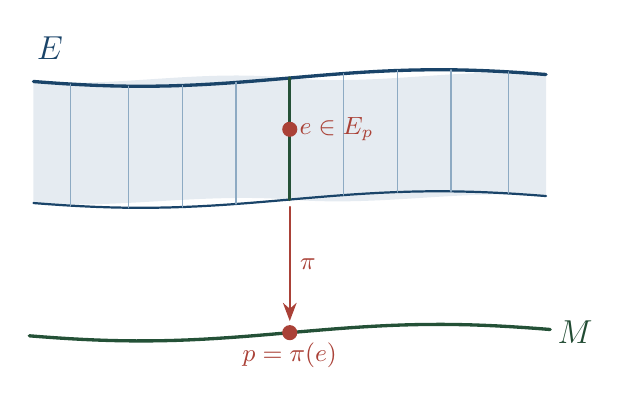
\begin{tikzpicture}[>=Stealth,scale=1.05,line cap=round]
\fill[manifoldblue!12] (-3.1,1.0)
 .. controls (-2.1,.92) and (-1.1,1.15) .. (0,1.04)
 .. controls (1.1,.94) and (2.1,1.18) .. (3.1,1.08)
 --(3.1,-.39)
 .. controls (2.1,-.30) and (1.1,-.52) .. (0,-.43)
 .. controls (-1.1,-.35) and (-2.1,-.55) .. (-3.1,-.47) --cycle;
\draw[manifoldblue!75!black,very thick]
 plot[domain=-3.1:3.1,samples=35] ({\x},{1.04+.10*sin(50*\x)});
\draw[manifoldblue!75!black,thick]
 plot[domain=-3.1:3.1,samples=35] ({\x},{-.43+.10*sin(50*\x)});
\foreach \xx in {-2.65,-1.95,-1.3,-.65,.65,1.3,1.95,2.65}
 \draw[manifoldblue!52,thin] (\xx,{-.43+.10*sin(50*\xx)})
 --(\xx,{1.04+.10*sin(50*\xx)});
\draw[manifoldgreen!65!black,very thick] (0,-.43)--(0,1.04);
\draw[manifoldgreen!65!black,very thick]
 plot[domain=-3.15:3.15,samples=40] ({\x},{-2.04+.10*sin(50*\x)});
\fill[manifoldred] (0,.42) circle (2.6pt) node[right,font=\small] {$e\in E_p$};
\fill[manifoldred] (0,-2.04) circle (2.6pt) node[below,font=\small] {$p=\pi(e)$};
\draw[->,thick,manifoldred] (0,-.52)--(0,-1.9)
 node[midway,right,font=\small] {$\pi$};
\node[manifoldblue!75!black,font=\large\bfseries] at (-2.9,1.4) {$E$};
\node[manifoldgreen!60!black,font=\large\bfseries] at (3.45,-2.03) {$M$};
\end{tikzpicture}
\caption{Lokalny obraz wiązki $\pi\colon E\to M$. Wyróżniono wektor $e$ i jego rzut $\pi(e)=p$. Włókna narysowano jako fragmenty prostych; ogólnie mają wymiar $k$.}
\label{fig:diagram-wiazki}
\end{figure}







Rysunek~\ref{fig:trywializacja} przedstawia lokalną trywializację
z Definicji~\ref{def:wiazka-wektorowa}: zachowuje ona punkt bazy
i jest liniowa na każdym włóknie.

\begin{figure}[ht]
\centering
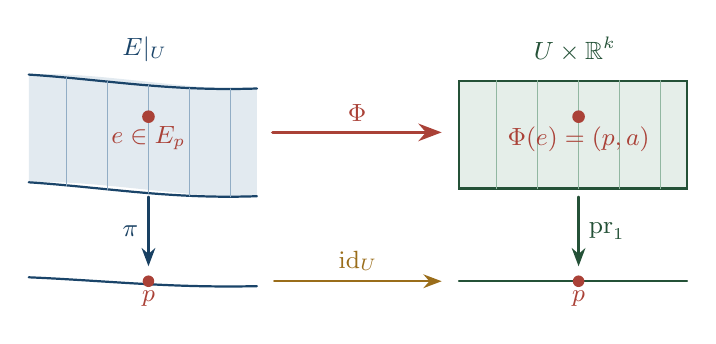
\begin{tikzpicture}[>=Stealth,scale=.95,line cap=round]
\fill[manifoldblue!13] (-4.4,1.16)
 .. controls (-3.55,1.22) and (-2.2,.93) .. (-1.35,.98)
 --(-1.35,-.46)
 .. controls (-2.2,-.51) and (-3.55,-.23) .. (-4.4,-.28) --cycle;
\draw[manifoldblue!75!black,thick]
 plot[domain=-4.4:-1.35,samples=25] ({\x},{1.08+.11*sin(52*\x)});
\draw[manifoldblue!75!black,thick]
 plot[domain=-4.4:-1.35,samples=25] ({\x},{-.36+.11*sin(52*\x)});
\foreach \xx in {-3.9,-3.35,-2.8,-2.25,-1.7}
 \draw[manifoldblue!50,thin] (\xx,{-.36+.11*sin(52*\xx)})
 --(\xx,{1.08+.11*sin(52*\xx)});
\fill[manifoldgreen!13] (1.35,-.36) rectangle (4.4,1.08);
\draw[manifoldgreen!65!black,thick] (1.35,-.36) rectangle (4.4,1.08);
\foreach \xx in {1.85,2.4,2.95,3.5,4.05}
 \draw[manifoldgreen!55,thin] (\xx,-.36)--(\xx,1.08);
\fill[manifoldred] (-2.8,.6) circle (2.4pt)
 node[below,font=\small] {$e\in E_p$};
\fill[manifoldred] (2.95,.6) circle (2.4pt)
 node[below,font=\small] {$\Phi(e)=(p,a)$};
\draw[->,very thick,manifoldred] (-1.14,.39)--(1.12,.39)
 node[midway,above,font=\small] {$\Phi$};
\draw[manifoldblue!75!black,thick]
 plot[domain=-4.4:-1.35,samples=25] ({\x},{-1.6+.07*sin(52*\x)});
\draw[manifoldgreen!65!black,thick] (1.35,-1.6)--(4.4,-1.6);
\fill[manifoldred] (-2.8,-1.6) circle (2.2pt) node[below,font=\small] {$p$};
\fill[manifoldred] (2.95,-1.6) circle (2.2pt) node[below,font=\small] {$p$};
\draw[->,manifoldblue!70!black,thick] (-2.8,-.47)--(-2.8,-1.4)
 node[midway,left,font=\small] {$\pi$};
\draw[->,manifoldgreen!65!black,thick] (2.95,-.47)--(2.95,-1.4)
 node[midway,right,font=\small] {$\operatorname{pr}_1$};
\draw[->,manifoldgold!75!black,thick] (-1.12,-1.6)--(1.12,-1.6)
 node[midway,above,font=\small] {$\mathrm{id}_U$};
\node[manifoldblue!75!black,font=\small\bfseries] at (-2.85,1.5) {$E|_U$};
\node[manifoldgreen!65!black,font=\small\bfseries] at (2.9,1.5) {$U\times\R^k$};
\end{tikzpicture}
\caption{Trywializacja $\Phi\colon E|_U\to U\times\R^k$ jest liniowa na włóknach i zachowuje punkt bazy: $\operatorname{pr}_1\circ\Phi=\pi$. Linie przedstawiają włókna schematycznie.}
\label{fig:trywializacja}
\end{figure}

\begin{definicja}[Sekcja wiązki wektorowej]
\index{sekcja wiazki wektorowej@Sekcja wiązki wektorowej}
Niech $\pi\colon E\to M$ będzie wiązką wektorową. \emph{Sekcją}
(inaczej: \emph{przekrojem}) wiązki $E$ nazywamy
gładkie odwzorowanie $s\colon M\to E$ spełniające $\pi\circ s=\id_M$.
Zatem dla każdego $p\in M$ mamy $s(p)\in E_p$. Sekcja wybiera dokładnie jeden wektor
z każdego włókna i robi to w sposób gładki.
\end{definicja}

\begin{figure}[ht]
\centering
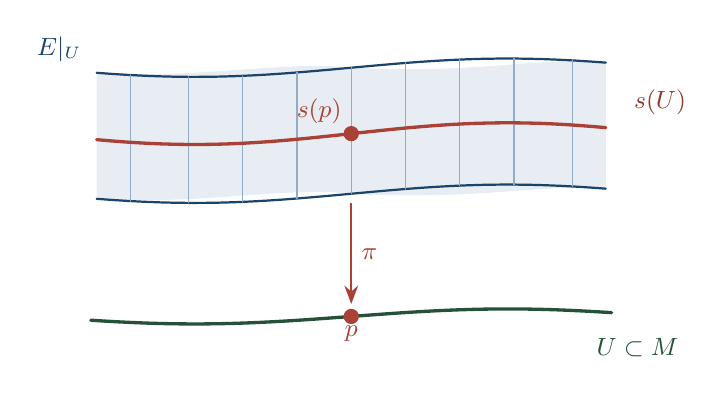
\begin{tikzpicture}[>=Stealth,scale=1.06,line cap=round]
\fill[manifoldblue!11] (-3.05,1.07)
 .. controls (-1.8,.99) and (-.8,1.22) .. (0,1.13)
 .. controls (1.6,1.05) and (2.2,1.27) .. (3.05,1.19)
 --(3.05,-.32)
 .. controls (2.2,-.26) and (1.6,-.46) .. (0,-.38)
 .. controls (-.8,-.29) and (-1.8,-.52) .. (-3.05,-.44) --cycle;
\draw[manifoldblue!75!black,thick]
 plot[domain=-3.05:3.05,samples=34] ({\x},{1.13+.11*sin(48*\x)});
\draw[manifoldblue!75!black,thick]
 plot[domain=-3.05:3.05,samples=34] ({\x},{-.38+.11*sin(48*\x)});
\foreach \xx in {-2.65,-1.95,-1.3,-.65,0,.65,1.3,1.95,2.65}
 \draw[manifoldblue!50,thin] (\xx,{-.38+.11*sin(48*\xx)})
 --(\xx,{1.13+.11*sin(48*\xx)});
\draw[manifoldgreen!65!black,very thick]
 plot[domain=-3.12:3.12,samples=38] ({\x},{-1.85+.09*sin(48*\x)});
\draw[manifoldred,very thick]
 plot[domain=-3.05:3.05,samples=40] ({\x},{.34+.13*sin(48*\x)});
\fill[manifoldred] (0,.34) circle (2.6pt) node[above left,font=\small] {$s(p)$};
\fill[manifoldred] (0,-1.85) circle (2.6pt) node[below,font=\small] {$p$};
\draw[->,manifoldred,thick] (0,-.5)--(0,-1.7)
 node[midway,right,font=\small] {$\pi$};
\node[font=\small\bfseries,manifoldred!85!black] at (3.7,.72) {$s(U)$};
\node[font=\small\bfseries,manifoldgreen!65!black] at (3.43,-2.22) {$U\subset M$};
\node[font=\small,manifoldblue!75!black] at (-3.5,1.35) {$E|_U$};
\end{tikzpicture}
\caption{Sekcja $s$ wybiera dokładnie jeden wektor $s(p)$ w każdym włóknie nad $p$. Czerwona krzywa przedstawia jej obraz nad pokazanym fragmentem $U$.}
\label{fig:sekcja}
\end{figure}

\begin{przyklad}[Sekcja zerowa]
Każda wiązka wektorowa posiada naturalną \emph{sekcję zerową} $s_0\colon M\to E,\ s_0(p)=0_p$,
gdzie $0_p$ jest wektorem zerowym we włóknie $E_p$.
Gładkość wynika z lokalnego zapisu $p\mapsto(p,0)$.
\end{przyklad}


\begin{przyklad}[Wiązka trywialna]
Najprostszym przykładem jest $E=M\times\R^k$ z $\pi=\mathrm{pr}_1$ i $\Psi=\id$ — wiązka ta
nosi nazwę \emph{trywialnej}.
\end{przyklad}

\begin{definicja}[Izomorfizm wiązek wektorowych]
\index{izomorfizm wiazek wektorowych@Izomorfizm wiązek wektorowych}
\label{def:izomorfizm-wiazek}
Niech
$
\pi_E\colon E\to M,
\
\pi_F\colon F\to M
$
będą wiązkami wektorowymi tego samego rzędu nad $M$.
\emph{Izomorfizmem wiązek wektorowych nad $M$} nazywamy
dyfeomorfizm
$
\Phi\colon E\to F
$
taki, że
$
\pi_F\circ\Phi=\pi_E,
$
oraz dla każdego $p\in M$ ograniczenie
$
\Phi_p:=\Phi|_{E_p}\colon E_p\to F_p
$
jest izomorfizmem liniowym.


Warunek
$
\pi_F\circ\Phi=\pi_E
$
oznacza, że $\Phi$ zachowuje punkt bazy: dla każdego $v\in E_p$
mamy
$
\Phi(v)\in F_p.
$
\end{definicja}


\begin{uwaga}
\index{wiazka wektorowa@Wiązka wektorowa!trywialnosc lokalna@trywialność lokalna}
\index{wiazka wektorowa@Wiązka wektorowa!trywialnosc globalna@trywialność globalna}
Każda wiązka wektorowa jest z definicji \emph{lokalnie trywialna}:
dla każdego $p\in M$ istnieje otwarte otoczenie $U\ni p$ takie, że
$
\pi^{-1}(U)\cong U\times\R^k
$
jako wiązki wektorowe nad $U$.

Nie każda wiązka lokalnie trywialna jest jednak globalnie trywialna.
Innymi słowy, z istnienia lokalnych izomorfizmów
$
\pi^{-1}(U)\cong U\times\R^k
$
nie wynika istnienie jednego globalnego izomorfizmu
$
E\cong M\times\R^k.
$
\end{uwaga}
\begin{przyklad}[Wstęga Möbiusa jako nietrywialna wiązka rzędu $1$]
\label{prz:mobius}
\index{wstega Mobiusa\@Wstęga Möbiusa}
\index{wiazka wektorowa\@Wiązka wektorowa!wstega Mobiusa\@wstęga Möbiusa}

Niech
$
M=S^1=\R/2\pi\Z.
$
Na przestrzeni $\R^2=\R\times\R$ definiujemy relację
\[
(x,t)\sim(y,s)
\quad\Longleftrightarrow\quad
\exists k\in\Z
\quad\text{takie, że}\quad
y=x+2\pi k,\qquad s=(-1)^k t.
\]
Definiujemy przestrzeń ilorazową
$
E:=\R^2/\sim.
$
Klasę równoważności punktu $(x,t)\in\R^2$ oznaczamy przez
$
[x,t].
$

Interpretacja tej definicji jest następująca:
przesunięcie pierwszej współrzędnej o jeden pełny obrót, czyli o $2\pi$,
powoduje zmianę znaku drugiej współrzędnej:
$
[x,t]=[x+2\pi,-t].
$
Po dwóch pełnych obrotach znak wraca do pierwotnego:
$
[x,t]=[x+4\pi,t].
$
Właśnie to odwrócenie znaku po jednym obejściu okręgu odpowiada
skręceniu charakterystycznemu dla wstęgi Möbiusa.

Definiujemy rzutowanie $\pi\colon E\longrightarrow S^1, \ \pi([x,t])=[x]$.
Jest ono dobrze określone, ponieważ jeśli
$
(x,t)\sim(y,s),
$
to
$
y=x+2\pi k
$
dla pewnego $k\in\Z$, a więc
$
[y]=[x]
\quad\text{w}\quad
\R/2\pi\Z=S^1.
$

\medskip
\emph{Lokalna trywialność poza punktem sklejenia.}

Niech $I\subset S^1$ będzie otwartym łukiem, który nie zawiera punktu $[0]$.
Możemy wtedy wybrać przedział $(a,b)\subset\R, \ b-a\leq2\pi$,
taki, że każdy punkt $p\in I$ ma dokładnie jednego reprezentanta
$x\in(a,b)$.

Definiujemy
\[
\Psi_I\colon \pi^{-1}(I)\longrightarrow I\times\R,
\qquad
\Psi_I([x,t])=([x],t),
\qquad x\in(a,b).
\]
Odwrotność ma postać $\Psi_I^{-1}([x],t)=[x,t], \ x\in(a,b)$.
Ponieważ na otwartym przedziale długości co najwyżej $2\pi$
nie trzeba przechodzić
przez punkt sklejenia, współrzędna włókna nie zmienia znaku i otrzymujemy
zwykłą lokalną trywializację.

\medskip
\emph{Lokalna trywialność w otoczeniu punktu $[0]$.}

Wybierzmy
$
0<\varepsilon<\pi
$
i rozważmy otwarty łuk
$
I_0:=\{[a]\in S^1:\,-\varepsilon<a<\varepsilon\}.
$
Każdy punkt tego łuku ma dokładnie jednego reprezentanta
$
a\in(-\varepsilon,\varepsilon).
$
Definiujemy odwrotność lokalnej trywializacji przez $\Psi_0^{-1}\colon I_0\times\R\longrightarrow \pi^{-1}(I_0)$,
\[
\Psi_0^{-1}([a],v)=
\begin{cases}
[a,v],& a\ge 0,\\[1mm]
[a+2\pi,-v],& a<0.
\end{cases}
\]

To jest właśnie miejsce, w którym pojawia się zmiana znaku.
Jeżeli $a\ge 0$, to wybieramy reprezentanta $a$ leżącego blisko $0$
z prawej strony i nic nie zmieniamy.
Jeżeli natomiast $a<0$, to aby opisać ten sam punkt okręgu za pomocą
reprezentanta z przedziału bliskiego $2\pi$, musimy zastąpić $a$
przez $a+2\pi$. Z definicji relacji równoważności mamy wtedy
$
[a,v]=[a+2\pi,-v].
$
A zatem przejście od reprezentanta $a$ do reprezentanta $a+2\pi$
wymusza zmianę współrzędnej włókna z $v$ na $-v$.
To nie jest dodatkowa konwencja, lecz bezpośrednia konsekwencja definicji
relacji
$
(x,t)\sim(x+2\pi,-t).
$

Odpowiadająca trywializacja ma postać
\[
\Psi_0([x,t])=
\begin{cases}
([x],t),& -\varepsilon<x<\varepsilon,\\[1mm]
([x-2\pi],-t),& 2\pi-\varepsilon<x<2\pi+\varepsilon.
\end{cases}
\]
W drugim przypadku odejmujemy $2\pi$, aby wrócić do reprezentanta
z przedziału $(-\varepsilon,\varepsilon)$, a współrzędna włókna
musi zmienić znak dokładnie z tego samego powodu co wyżej.

\medskip
\emph{Funkcje przejścia.}

Wybierzmy dwa otwarte łuki $U_0,U_1\subset S^1$, które pokrywają okrąg,
przy czym $U_0$ jest małym łukiem wokół punktu $[0]$, a $U_1=S^1\setminus\{[0]\}$.
Na $U_1$ używamy trywializacji
$
\Psi_1([x,t])=([x],t),
\ x\in(0,2\pi),
$
natomiast na $U_0$ trywializacji $\Psi_0$ zdefiniowanej wyżej.

Przecięcie $U_0\cap U_1$ ma dwie składowe spójne:
jedną w pobliżu punktu $[0]$ od strony dodatniej,
oraz drugą w pobliżu tego samego punktu od strony ujemnej
(czyli po identyfikacji: w pobliżu $2\pi$).

Na składowej dodatniej oba opisy używają tego samego reprezentanta $x$,
więc współrzędna włókna się nie zmienia:
$
v\longmapsto v.
$
Funkcja przejścia jest tam więc równa
$
g=+1.
$

Na składowej ujemnej jedna trywializacja używa reprezentanta bliskiego $0$,
a druga reprezentanta bliskiego $2\pi$.
Przejście między tymi reprezentantami odbywa się przez dodanie lub odjęcie
$2\pi$, a więc z definicji relacji
$
[x,t]=[x+2\pi,-t]
$
współrzędna włókna musi zmienić znak:
$
v\longmapsto -v.
$
Funkcja przejścia jest tam zatem równa
$
g=-1.
$

To dokładnie pokazuje, gdzie geometrycznie pojawia się skręt:
lokalnie mamy produkt $I\times\R$, lecz przy obejściu bazy dookoła
współrzędna włókna wraca z przeciwnym znakiem.

\medskip
Sprawdźmy jeszcze, że otrzymane opisy zgadzają się z topologią
ilorazową $E$. Niech $q:\R^2\to E$ będzie odwzorowaniem ilorazowym.
Jest ono otwarte: dla otwartego $A\subset\R^2$ przeciwobraz
$q^{-1}(q(A))$ jest sumą obrazów $A$ przez homeomorfizmy
$(x,t)\mapsto(x+2\pi k,(-1)^k t)$, $k\in\Z$.
Jeżeli otwarty łuk $I\subset S^1$ jest obrazem przedziału
$J\subset\R$ długości mniejszej niż $2\pi$, to
$q|_{J\times\R}:J\times\R\to\pi^{-1}(I)$ jest bijekcją:
każda klasa ma reprezentanta o pierwszej współrzędnej w $J$,
a dwóch takich reprezentantów nie może różnić przesunięcie
o niezerową wielokrotność $2\pi$. Jest to homeomorfizm,
bo jest ciągły i otwarty. Przejścia między tymi współrzędnymi
mają lokalnie postać
$(x,t)\mapsto(x+2\pi k,(-1)^k t)$ ze stałym $k$,
więc są gładkie.

Punkty nad różnymi punktami bazy rozdzielają przeciwobrazy
rozłącznych łuków w $S^1$. Dwa różne punkty tego samego
włókna rozdzielają otoczenia w jednym z powyższych
otwartych iloczynów. Zatem $E$ jest Hausdorffa.
Przeliczalne pokrycie okręgu takimi łukami i przeliczalne
bazy iloczynów $J\times\R$ dają drugi aksjomat
przeliczalności. W konsekwencji $E$ jest gładką
dwuwymiarową rozmaitością, a odwzorowanie
$
\pi\colon E\to S^1
$
jest gładką rzeczywistą wiązką liniową rzędu $1$.

\end{przyklad}

\begin{figure}[h]
\centering
\begin{minipage}{0.43\textwidth}
\centering
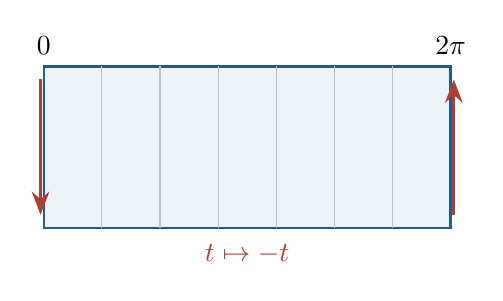
\begin{tikzpicture}[>=Stealth,scale=0.82]
  \fill[manifoldblue!8] (0,-1.25) rectangle (6.3,1.25);
  \draw[thick,manifoldblue] (0,-1.25) rectangle (6.3,1.25);
  \foreach \x in {0.9,1.8,2.7,3.6,4.5,5.4}
    \draw[manifoldblue!35] (\x,-1.25)--(\x,1.25);
  \draw[very thick,->,manifoldred] (-0.05,1.05) -- (-0.05,-1.05);
  \draw[very thick,->,manifoldred] (6.35,-1.05) -- (6.35,1.05);
  \node[above] at (0,1.28) {$0$};
  \node[above] at (6.3,1.28) {$2\pi$};
  \node[manifoldred] at (3.15,-1.65) {$t\mapsto-t$};
\end{tikzpicture}

\smallskip
\small (a) Prostokąt przed sklejeniem
\end{minipage}
\hfill
\begin{minipage}{0.53\textwidth}
\centering
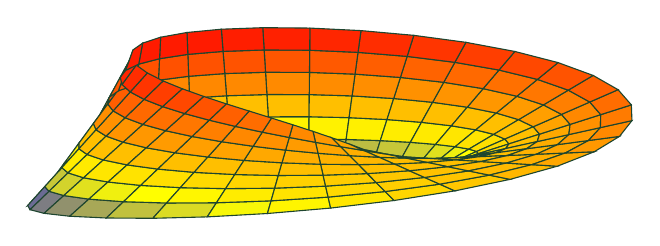
\begin{tikzpicture}
\begin{axis}[
  width=\linewidth,
  height=5.4cm,
  view={55}{25},
  axis lines=none,
  ticks=none,
  z buffer=sort,
  clip=false
]
\addplot3[
  surf,
  shader=faceted,
  faceted color=manifoldgreen!55!black,
  draw=manifoldgreen!70!black,
  domain=0:360,
  y domain=-0.55:0.55,
  samples=34,
  samples y=8
]
({(1+y*cos(x/2))*cos(x)},
 {(1+y*cos(x/2))*sin(x)},
 {y*sin(x/2)});
\end{axis}
\end{tikzpicture}

\smallskip
\small (b) Model geometryczny w $\R^3$
\end{minipage}
\caption{Wstęga Möbiusa: (a) konstrukcja przez sklejenie boków prostokąta z
odwróceniem współrzędnej włókna, (b) odpowiadająca jej klasyczna powierzchnia
zanurzona w $\R^3$. Parametryzacja w części (b) ma postać
$x=(1+t\cos(\theta/2))\cos\theta$,
$y=(1+t\cos(\theta/2))\sin\theta$,
$z=t\sin(\theta/2)$. Rysunek pokazuje tylko pas $|t|\leq0.55$;
w całej wiązce wektorowej $t$ przebiega $\R$.}
\label{fig:mobius}
\end{figure}

\begin{stwierdzenie}[Brak globalnej trywializacji]
\label{prop:mobius-nietrywialna}
\index{wstega Mobiusa\@Wstęga Möbiusa!nietrywialnosc\@nietrywialność}

Wiązka
$
\pi\colon E\to S^1
$
z Przykładu~\ref{prz:mobius} nie jest izomorficzna
z wiązką trywialną
$
S^1\times\R\to S^1.
$
Inaczej mówiąc, nie istnieje globalna trywializacja
$
E\cong S^1\times\R
$
jako wiązek nad $S^1$.
\end{stwierdzenie}

\begin{proof}
Pokażemy najpierw, że każda ciągła sekcja wiązki $E$
musi gdzieś znikać.

Niech
$
s\colon S^1\to E
$
będzie ciągłą sekcją, czyli
$
\pi\circ s=\operatorname{id}_{S^1}.
$
Podnosząc ją do funkcji na $\R$, możemy zapisać
$
s([x])=[x,f(x)]
$
dla pewnej ciągłej funkcji
$
f\colon\R\to\R.
$
Ponieważ
$
[x]=[x+2\pi]
\quad\text{w }S^1,
$
musimy mieć
$
s([x])=s([x+2\pi]).
$
To znaczy
$
[x,f(x)]=[x+2\pi,f(x+2\pi)].
$
Z definicji relacji równoważności wynika stąd
$
f(x+2\pi)=-f(x)
\ \text{dla każdego }x\in\R.
$

Załóżmy teraz, że sekcja $s$ jest nigdzie niezerowa.
Wtedy
$
f(x)\neq 0
\ \text{dla każdego }x\in\R.
$
Jako funkcja ciągła na spójnym zbiorze $\R$,
funkcja $f$ musi mieć stały znak.
W szczególności liczby $f(0)$ i $f(2\pi)$
muszą mieć ten sam znak.

Z drugiej strony z warunku
$
f(2\pi)=-f(0)
$
wynika, że mają znaki przeciwne, o ile tylko $f(0)\neq 0$.
To sprzeczność. Zatem każda ciągła sekcja wiązki $E$
musi mieć co najmniej jedno zero.

Tymczasem wiązka trywialna
$
S^1\times\R\to S^1
$
ma globalną nigdzie niezerową sekcję, na przykład
$
s_1(p)=(p,1).
$

Gdyby istniał izomorfizm wiązek
$
\Phi\colon S^1\times\R\longrightarrow E,
$
to sekcja
$
\Phi\circ s_1
$
byłaby globalną nigdzie niezerową sekcją wiązki $E$.
Jest to niemożliwe na mocy poprzedniego argumentu.

Otrzymujemy sprzeczność. Zatem globalna trywializacja nie istnieje.
\end{proof}

\begin{uwaga}[Znaczenie topologiczne]
Wstęga Möbiusa jest podstawowym przykładem sytuacji, w której
lokalna trywialność nie pociąga za sobą globalnej trywialności.
Na każdym dostatecznie małym łuku
$
I\subset S^1
$
mamy izomorfizm
$
\pi^{-1}(I)\cong I\times\R,
$
jednak nie istnieje jeden globalny izomorfizm
$
E\cong S^1\times\R.
$

Źródłem tej przeszkody jest dokładnie zmiana znaku
$
t\longmapsto -t
$
po jednym pełnym obejściu bazy.
To ona powoduje, że lokalne układy współrzędnych na włóknach
nie mogą zostać sklejone w jeden globalny wybór współrzędnej.
\end{uwaga}

\begin{przyklad}[Wiązka tautologiczna nad $\mathbb{RP}^1$]
\label{prz:tautologiczna-rp1}
\index{wiazka tautologiczna\@Wiązka tautologiczna}
\index{przestrzen rzutowa\@Przestrzeń rzutowa!wiazka tautologiczna\@wiązka tautologiczna}

Przykład wstęgi Möbiusa ma naturalny związek z rzeczywistą
przestrzenią rzutową $\mathbb{RP}^1$.

Przypomnijmy, że $\mathbb{RP}^1$ jest przestrzenią
jednowymiarowych podprzestrzeni liniowych $\R^2$.
Jej punkty zapisujemy w postaci
$
[x_1:x_2],
\ (x_1,x_2)\in\R^2\setminus\{0\},
$
przy czym
$
[x_1:x_2]=[\lambda x_1:\lambda x_2]
\ \text{dla każdego }\lambda\in\R\setminus\{0\}.
$


Każdemu punktowi $[x]\in\mathbb{RP}^1$,
gdzie $x=(x_1,x_2)\neq0$, odpowiada prosta $L_{[x]}:=\operatorname{span}(x) =\{tx:t\in\R\}\subset\R^2$.
Definicja ta nie zależy od wyboru reprezentanta,
ponieważ
$
\operatorname{span}(\lambda x)
=\operatorname{span}(x)
\ (\lambda\neq0).
$

Definiujemy przestrzeń całkowitą
\[
\boxed{
\gamma^1
:=
\bigl\{
([x],v)\in\mathbb{RP}^1\times\R^2:
v\in\operatorname{span}(x)
\bigr\}
}
\]
oraz rzutowanie
\[
\pi_\gamma\colon\gamma^1\longrightarrow\mathbb{RP}^1,
\qquad
\pi_\gamma([x],v)=[x].
\]

Włókno nad punktem $[x]$ ma zatem postać
$
\gamma^1_{[x]}
=
\bigl\{
([x],v):v\in\operatorname{span}(x)
\bigr\}.
$
Po utożsamieniu włókna z jego drugą współrzędną
otrzymujemy
$
\gamma^1_{[x]}\cong\operatorname{span}(x)\cong\R.
$
Poniższe trywializacje pokażą, że otrzymujemy
rzeczywistą wiązkę liniową rzędu $1$,
nazywaną \emph{wiązką tautologiczną}
lub \emph{kanoniczną wiązką liniową} nad $\mathbb{RP}^1$.

Geometrycznie konstrukcja polega na tym, że nad
każdym punktem przestrzeni rzutowej umieszczamy
dokładnie tę prostą w $\R^2$, którą dany punkt
reprezentuje.

\medskip
\emph{Lokalne trywializacje.}

Rozważmy standardowe otwarte podzbiory
$
U_i:=\{[x_1:x_2]\in\mathbb{RP}^1:x_i\neq0\},\ i=1,2.
$


Na $U_1$ używamy współrzędnej $z=\frac{x_2}{x_1}, \ [x_1:x_2]=[1:z]$.
Prosta odpowiadająca punktowi $[1:z]$
jest rozpięta przez wektor $(1,z)$.
Wybierzmy na niej wektor jednostkowy $u_1(z):=\frac{(1,z)}{\sqrt{1+z^2}}$.

Każdy wektor należący do tej prostej
można jednoznacznie zapisać jako
$
v=t\,u_1(z),
\ t\in\R.
$
Ponieważ $u_1(z)$ jest jednostkowy,
współczynnik ten wynosi
$s
t=\langle v,u_1(z)\rangle,
$
gdzie $\langle\cdot,\cdot\rangle$
oznacza standardowy iloczyn skalarny w $\R^2$.

Definiujemy lokalną trywializację
$
\Psi_1\colon
\pi_\gamma^{-1}(U_1)\longrightarrow U_1\times\R
$
wzorem $\Psi_1([1:z],v) = \bigl([1:z],\langle v,u_1(z)\rangle\bigr)$.
Jej odwrotność ma postać $\Psi_1^{-1}([1:z],t) = \bigl([1:z],t\,u_1(z)\bigr)$.

Analogicznie na $U_2$ używamy współrzędnej $w=\frac{x_1}{x_2}, \ [x_1:x_2]=[w:1]$,
i wybieramy wektor jednostkowy $u_2(w):=\frac{(w,1)}{\sqrt{1+w^2}}$.
Otrzymujemy drugą lokalną trywializację $\Psi_2([w:1],v) = \bigl([w:1],\langle v,u_2(w)\rangle\bigr)$,
której odwrotność jest dana przez $\Psi_2^{-1}([w:1],t) = \bigl([w:1],t\,u_2(w)\bigr)$.

Sprawdźmy strukturę gładką przestrzeni całkowitej,
którą na razie traktujemy jako podzbiór
$\mathbb{RP}^1\times\R^2$ z topologią podprzestrzeni.
Nad $U_1$ współrzędne $(z,v_1,v_2)$ spełniają
$v_2=zv_1$. Jest to wykres gładkiej funkcji
$(z,v_1)\mapsto zv_1$, a zatem gładka powierzchnia
w $U_1\times\R^2$. W tych współrzędnych
$t=\langle v,u_1(z)\rangle=v_1\sqrt{1+z^2}$,
więc $\Psi_1$ i jej odwrotność są gładkie.
Analogicznie nad $U_2$ mamy wykres $v_1=wv_2$
oraz $t=v_2\sqrt{1+w^2}$. Obszary $U_1,U_2$
pokrywają $\mathbb{RP}^1$, toteż $\gamma^1$
jest gładką dwuwymiarową podrozmaitością produktu,
a $\Psi_1,\Psi_2$ są lokalnymi trywializacjami
liniowymi na każdym włóknie.

\medskip
\emph{Funkcje przejścia i zmiana znaku.}

Obliczmy funkcję przejścia między
trywializacjami $\Psi_1$ i $\Psi_2$.

Na przecięciu $U_1\cap U_2$ mamy $z\neq0, \ w=\frac1z$.
Zatem
$
u_2(w)=\operatorname{sgn}(z)\,u_1(z)
$
oraz
$
u_2(1/z)=\operatorname{sgn}(z)\,u_1(z).
$

Wyjaśnijmy jej znaczenie.

Jeżeli $z>0$, to
$
u_2(1/z)=u_1(z),
$
a więc oba lokalnie wybrane wektory jednostkowe
mają ten sam zwrot.

Jeżeli natomiast $z<0$, to
$
u_2(1/z)=-u_1(z).
$
Oba wektory rozpinają tę samą prostą,
ale mają przeciwne zwroty.

Niech teraz
$
v=t_1u_1(z)=t_2u_2(1/z).
$
Z poprzedniej równości dostajemy
$
t_1u_1(z)
=
t_2\operatorname{sgn}(z)u_1(z),
$
a zatem
$
t_2=\operatorname{sgn}(z)t_1.
$

Funkcja przejścia ma więc postać
\[
\boxed{
g_{21}([1:z])
=
\begin{cases}
+1,&z>0,\\
-1,&z<0.
\end{cases}
}
\]

Przecięcie $U_1\cap U_2$ ma dwie składowe
spójności, odpowiadające $z>0$ oraz $z<0$.
Na jednej z nich współrzędna włókna
pozostaje niezmieniona, a na drugiej
zmienia znak.

Zmiana znaku nie oznacza zmiany samego
wektora $v\in\R^2$.
Wektor ten pozostaje ten sam.
Zmienia się jedynie jego współrzędna
względem innego wyboru wektora jednostkowego
rozpinającego tę samą prostą.

W szczególności
$
v=t\,u=(-t)(-u).
$
Ta prosta równość algebraiczna wyjaśnia
geometrycznie występowanie funkcji przejścia
równej $-1$.

\medskip
\emph{Identyfikacja $\mathbb{RP}^1$ z okręgiem.}

Pokażemy teraz, że wiązka $\gamma^1$
jest izomorficzna z wstęgą Möbiusa
skonstruowaną w Przykładzie~\ref{prz:mobius}.


Zdefiniujmy odwzorowanie
$
F\colon S^1\longrightarrow\mathbb{RP}^1
$
wzorem $F([\theta]) = [\cos(\theta/2):\sin(\theta/2)]$.

Najpierw sprawdźmy, że jest ono dobrze określone.
Jeżeli
$
[\theta]=[\varphi]\in S^1,
$
to
$
\varphi=\theta+2\pi k
$
dla pewnego $k\in\Z$.
Wówczas
\[
\begin{aligned}
\cos(\varphi/2)
&=\cos(\theta/2+\pi k)
=(-1)^k\cos(\theta/2),\\
\sin(\varphi/2)
&=\sin(\theta/2+\pi k)
=(-1)^k\sin(\theta/2).
\end{aligned}
\]
Ponieważ w przestrzeni rzutowej
utożsamiamy niezerowe wielokrotności
tego samego wektora, otrzymujemy
$
[\cos(\varphi/2):\sin(\varphi/2)]
=
[\cos(\theta/2):\sin(\theta/2)].
$

Pokażemy, że $F$ jest dyfeomorfizmem.

Różnowartościowość wynika z faktu, że
jeśli
$
[\cos(\theta/2):\sin(\theta/2)]
=
[\cos(\varphi/2):\sin(\varphi/2)],
$
to odpowiadające im wektory jednostkowe
różnią się co najwyżej znakiem:
\[
\begin{pmatrix}
\cos(\varphi/2)\\
\sin(\varphi/2)
\end{pmatrix}
=
\pm
\begin{pmatrix}
\cos(\theta/2)\\
\sin(\theta/2)
\end{pmatrix}.
\]
Stąd
$
\frac{\varphi}{2}
=
\frac{\theta}{2}+\pi k
$
dla pewnego $k\in\Z$, czyli
$
\varphi=\theta+2\pi k.
$
A zatem $[\varphi]=[\theta]$.

Aby wykazać surjektywność, weźmy dowolny
punkt $[x_1:x_2]\in\mathbb{RP}^1$.
Normalizując jego reprezentanta, możemy zapisać $\frac{(x_1,x_2)}{\sqrt{x_1^2+x_2^2}} = (\cos\alpha,\sin\alpha)$
dla pewnego $\alpha\in\R$.
Wtedy
$
F([2\alpha])
=
[\cos\alpha:\sin\alpha]
=
[x_1:x_2].
$

Dla pełności wskażmy również gładką
odwrotność. Utożsamiając $S^1$
z okręgiem jednostkowym w $\mathbb C$,
otrzymujemy wzór
\[
\boxed{
F^{-1}([x_1:x_2])
=
\frac{(x_1+ix_2)^2}{x_1^2+x_2^2}.
}
\]
Wyrażenie po prawej stronie należy do $S^1$,
ponieważ jego moduł wynosi $1$.
Nie zależy ono od reprezentanta:
zastąpienie $(x_1,x_2)$ przez
$(\lambda x_1,\lambda x_2)$ mnoży
licznik i mianownik przez $\lambda^2$.

Jeżeli
$
(x_1,x_2)=(\cos\alpha,\sin\alpha),
$
to
$
F^{-1}([x_1:x_2])
=(\cos\alpha+i\sin\alpha)^2
=e^{2i\alpha}.
$
Widzimy więc, że jest to rzeczywiście
odwrotność $F$.

Zarówno $F$, jak i $F^{-1}$
są gładkie w lokalnych współrzędnych,
a zatem
$
S^1\cong\mathbb{RP}^1
$
jako rozmaitości gładkie.

\medskip
\emph{Jawny izomorfizm wiązek.}

Dla $\theta\in\R$ oznaczmy
\[
u(\theta)
:=
\begin{pmatrix}
\cos(\theta/2)\\
\sin(\theta/2)
\end{pmatrix}.
\]
Jest to wektor jednostkowy rozpinający
prostą odpowiadającą punktowi $F([\theta])$.

Zdefiniujmy odwzorowanie
$
\Phi\colon E\longrightarrow\gamma^1
$
wzorem
\[
\Phi([\theta,t])
=
\bigl(
[\cos(\theta/2):\sin(\theta/2)],
t\,u(\theta)
\bigr).
\]

Wartość $\Phi([\theta,t])$ rzeczywiście
należy do $\gamma^1$, ponieważ
$
t\,u(\theta)
\in\operatorname{span}(u(\theta)).
$

Sprawdźmy dokładnie, że $\Phi$
jest dobrze określone na klasach równoważności.

Jeżeli
$
(\theta,t)\sim(\varphi,s),
$
to dla pewnego $k\in\Z$ mamy
$
\varphi=\theta+2\pi k,
\ 
s=(-1)^k t.
$
Jednocześnie
$
u(\varphi)
=
u(\theta+2\pi k)
=
(-1)^k u(\theta).
$
Stąd
$
s\,u(\varphi)=t\,u(\theta).
$
Ponadto
$
[u(\varphi)]=[u(\theta)]
\ \text{w }\mathbb{RP}^1.
$
W konsekwencji
$
\Phi([\varphi,s])=\Phi([\theta,t]).
$
Odwzorowanie $\Phi$ jest więc
dobrze określone.

W szczególności dla jednego pełnego obrotu
otrzymujemy rachunek
\[
\begin{aligned}
\Phi([\theta+2\pi,-t])
&=
\bigl([u(\theta+2\pi)],-t\,u(\theta+2\pi)\bigr)\\
&=
\bigl([-u(\theta)],(-t)(-u(\theta))\bigr)\\
&=
\bigl([u(\theta)],t\,u(\theta)\bigr)\\
&=\Phi([\theta,t]).
\end{aligned}
\]
Widzimy zatem, że zmiana znaku
współrzędnej włókna w definicji wstęgi Möbiusa
jest dokładnie kompensowana zmianą znaku
wektora jednostkowego reprezentującego
punkt przestrzeni rzutowej.

Odwzorowanie $\Phi$ zachowuje rzutowania,
gdyż
\[
\begin{aligned}
\pi_\gamma(\Phi([\theta,t]))
&=[\cos(\theta/2):\sin(\theta/2)]\\
&=F([\theta])\\
&=F(\pi([\theta,t])).
\end{aligned}
\]

Otrzymujemy więc przemienny diagram
\begin{center}
\begin{tikzcd}
E \arrow[r,"\Phi"] \arrow[d,"\pi"']
&
\gamma^1 \arrow[d,"\pi_\gamma"]
\\
S^1 \arrow[r,"F"']
&
\mathbb{RP}^1
\end{tikzcd}
\end{center}
Pokażemy teraz, że $\Phi$ jest bijekcją.
Niech
$
([x],v)\in\gamma^1.
$
Wybierzmy jednostkowy wektor $u$
rozpinający prostą $[x]$.
Możemy zapisać
$
u=(\cos\alpha,\sin\alpha)
$
dla pewnego $\alpha\in\R$.
Ponieważ $v\in\operatorname{span}(u)$,
istnieje dokładnie jedna liczba $t\in\R$
taka, że
$
v=tu.
$
Jest nią
$
t=\langle v,u\rangle.
$
Wówczas
$
\Phi([2\alpha,t])
=
([u],tu)
=
([x],v),
$
co dowodzi surjektywności.

Sprawdźmy również, że otrzymana klasa
$[2\alpha,t]\in E$ nie zależy od wyboru
wektora jednostkowego $u$.

Na tej samej prostej istnieją dokładnie
dwa wektory jednostkowe: $u$ oraz $-u$.
Jeżeli zastąpimy $u$ przez $-u$, to możemy
zastąpić $\alpha$ przez $\alpha+\pi$,
natomiast współczynnik $t$ przez $-t$:
$
v=tu=(-t)(-u).
$
Otrzymujemy wtedy parę
$
(2\alpha+2\pi,-t),
$
która jest równoważna z $(2\alpha,t)$,
ponieważ
$
(2\alpha,t)\sim(2\alpha+2\pi,-t).
$
Dodanie do $\alpha$ całkowitej wielokrotności
$2\pi$ również nie zmienia klasy w $E$.

Możemy zatem zdefiniować odwrotność $\Phi^{-1}([x],v) = [2\alpha,\langle v,u\rangle]$,
gdzie $u=(\cos\alpha,\sin\alpha)$
jest dowolnym wektorem jednostkowym
rozpinającym $[x]$.

Wykazaliśmy, że wzór ten nie zależy
od dokonanych wyborów.
Bezpośrednio otrzymujemy
\[
\Phi^{-1}\circ\Phi=\operatorname{id}_E,
\qquad
\Phi\circ\Phi^{-1}=\operatorname{id}_{\gamma^1}.
\]

Pozostaje uzasadnić gładkość.

Wybierzmy dostatecznie mały otwarty łuk
$I\subset S^1$, na którym można gładko
wybrać reprezentanta kąta $\theta$.
Na $\pi^{-1}(I)$ używamy trywializacji
wstęgi Möbiusa zapisującej każdy punkt
jednoznacznie jako $[\theta,t]$.

Na odpowiadającym mu obszarze $F(I)\subset\mathbb{RP}^1$
wybieramy gładki wektor jednostkowy
$
u(F([\theta]))=u(\theta).
$
Otrzymujemy wówczas trywializację
wiązki tautologicznej $([x],v)\longmapsto ([x],\langle v,u([x])\rangle)$.

W tych lokalnych trywializacjach
odwzorowanie $\Phi$ ma szczególnie prostą postać:
$
([\theta],t)\longmapsto(F([\theta]),t).
$
Jest więc gładkie, ponieważ $F$
jest dyfeomorfizmem.
Jego lokalna odwrotność ma postać
$
([x],t)\longmapsto(F^{-1}([x]),t)
$
i również jest gładka.

Ponadto na każdym włóknie $\Phi$
jest izomorfizmem liniowym:
$
t\longmapsto t\,u(\theta).
$

Ostatecznie $\Phi$ jest izomorfizmem
gładkich wiązek wektorowych nad
dyfeomorfizmem baz $F$:
\[
(E\xrightarrow{\pi}S^1)
\cong
(\gamma^1\xrightarrow{\pi_\gamma}\mathbb{RP}^1).
\]
Definicja~\ref{def:izomorfizm-wiazek} dotyczy wiązek
nad tą samą bazą; tutaj utożsamiamy bazy przez $F$,
a równanie $\pi_\gamma\circ\Phi=F\circ\pi$
zastępuje warunek zachowania punktu bazy.

\medskip
\emph{Geometryczna interpretacja skręcenia.}

Wyjaśnijmy jeszcze, dlaczego w tej konstrukcji
naturalnie pojawia się wstęga Möbiusa,
a nie wiązka trywialna.

Punkt $F([\theta]) = [\cos(\theta/2):\sin(\theta/2)]$
reprezentuje prostą przechodzącą przez początek
układu współrzędnych, tworzącą z dodatnią
półosią poziomą kąt $\theta/2$.

Kiedy $\theta$ przebiega przedział
$[0,2\pi]$, prosta wykonuje obrót o kąt $\pi$.
Jest to pełne obejście przestrzeni $\mathbb{RP}^1$,
ponieważ proste rozpięte przez $u$ i $-u$
są identyczne.

Jednak wybrany w sposób ciągły
wektor jednostkowy
$
u(\theta)
=
(\cos(\theta/2),\sin(\theta/2))
$
nie wraca do swojej początkowej wartości: $u(0)=(1,0),\ u(2\pi)=(-1,0)=-u(0)$.

Aby ten sam wektor $v$ we włóknie
przedstawić po pełnym obejściu bazy,
jego współczynnik musi więc zmienić znak:
$
v=t\,u(0)=(-t)\,u(2\pi).
$
Otrzymujemy dokładnie identyfikację
$
(0,t)\sim(2\pi,-t)
$
charakterystyczną dla wstęgi Möbiusa.

\medskip
\emph{Nietrywialność wiązki tautologicznej.}

Z wykazanego izomorfizmu i
Stwierdzenia~\ref{prop:mobius-nietrywialna}
wynika już, że $\gamma^1$ nie jest trywialna.
Można to również zobaczyć bezpośrednio
z jej geometrycznej konstrukcji.

Przypuśćmy, że istnieje globalna
nigdzie niezerowa ciągła sekcja
$
s\colon\mathbb{RP}^1\longrightarrow\gamma^1.
$
Dla $\theta\in[0,2\pi]$ możemy zapisać $s(F([\theta])) = \bigl(F([\theta]),a(\theta)u(\theta)\bigr)$,
gdzie $a\colon[0,2\pi]\to\R$
jest funkcją ciągłą.

Ponieważ
$
F([0])=F([2\pi]),
$
wartości przekroju na końcach przedziału
muszą być równe:
$
a(0)u(0)=a(2\pi)u(2\pi).
$
Korzystając z równości
$
u(2\pi)=-u(0),
$
otrzymujemy
$
a(0)u(0)=-a(2\pi)u(0),
$
a więc
$
a(2\pi)=-a(0).
$

Z twierdzenia o wartości pośredniej
wynika, że funkcja $a$ musi mieć zero
w przedziale $[0,2\pi]$.
Istnieje zatem $\theta_0$ takie, że
$
a(\theta_0)=0,
$
czyli
$
s(F([\theta_0]))
=
(F([\theta_0]),0).
$
Jest to sprzeczne z założeniem,
że przekrój jest nigdzie niezerowy.

Tymczasem każda trywialna wiązka
liniowa rzędu $1$ posiada globalny
nigdzie niezerowy przekrój.

W konsekwencji
$
\gamma^1\not\cong\mathbb{RP}^1\times\R
$
jako wiązki wektorowe nad $\mathbb{RP}^1$.

Wiązka tautologiczna nad $\mathbb{RP}^1$
jest więc dokładnie tą samą
nietrywialną wiązką liniową,
którą geometrycznie opisuje wstęga Möbiusa.
\end{przyklad}

\subsection*{Wiązka styczna}

Pokażemy, że zbiór $TM:=\bigsqcup_{p\in M}T_pM$
można w naturalny sposób wyposażyć w strukturę rozmaitości gładkiej
wymiaru $2n$, tak by rzutowanie $\pi\colon TM\to M, \ \pi(v)=p \quad\text{dla }v\in T_pM$,
było wiązką wektorową rzędu $n$.
Punkt $p=\pi(v)$ nazywamy \emph{podstawą}, natomiast
$T_pM=\pi^{-1}(p)$ jest włóknem wiązki stycznej nad $p$.

Niech $\{(U_\alpha,\varphi_\alpha)\}$ będzie atlasem na $M$,
$\varphi_\alpha=(x^1_\alpha,\dots,x^n_\alpha)$.
Definiujemy $\tilde U_\alpha:=\pi^{-1}(U_\alpha)\subseteq TM$
oraz
\[
\tilde\varphi_\alpha\colon
\tilde U_\alpha\to
\varphi_\alpha(U_\alpha)\times\R^n\subseteq\R^{2n},
\]
\[
\tilde\varphi_\alpha\Big(
\sum_{i=1}^n v^i
\left.\frac{\partial}{\partial x^i_\alpha}\right|_p
\Big)
:=
(\varphi_\alpha(p),v^1,\dots,v^n).
\]

Każde $\tilde\varphi_\alpha$ jest bijekcją na $\varphi_\alpha(U_\alpha)\times\R^n$
(dla ustalonego $p$, współrzędne $v^i$ względem bazy $\{\partial/\partial x^i_\alpha|_p\}$
wyznaczają bijekcję liniową $T_pM\to\R^n$).

Z reguły transformacji~\eqref{eq:transformacja-derywacji} wynika,
że dla $x\in\varphi_\alpha(U_\alpha\cap U_\beta)$ i $v\in\R^n$
odwzorowanie przejścia ma postać
\[
\big(\tilde\varphi_\beta\circ\tilde\varphi_\alpha^{-1}\big)(x,v)=\Big(
(\varphi_\beta\circ\varphi_\alpha^{-1})(x),\ D(\varphi_\beta\circ\varphi_\alpha^{-1})(x)
\cdot v\Big).
\]
Najpierw określamy topologię na $TM$: zbiór $A\subset TM$
jest otwarty wtedy i tylko wtedy, gdy każdy
$\tilde\varphi_\alpha(A\cap\tilde U_\alpha)$ jest otwarty.
Zmiany współrzędnych powyżej są homeomorfizmami, a ich dziedziny
$\varphi_\alpha(U_\alpha\cap U_\beta)\times\R^n$ są otwarte.
Wynika stąd, że $\tilde U_\alpha$ są otwarte, a
$\tilde\varphi_\alpha$ są homeomorfizmami: obraz dowolnego otwartego
zbioru z jednej mapy jest otwarty także w każdej nakładającej się mapie.
Rzutowanie $\pi$ jest ciągłe, bo lokalnie ma postać $(x,v)\mapsto x$.
Gładkość zmiany współrzędnych wynika z reguły
\eqref{eq:transformacja-derywacji}. Zatem $\{(\tilde
U_\alpha,\tilde\varphi_\alpha)\}$ jest atlasem na $TM$. Punkty o różnych
podstawach rozdzielają przeciwobrazy rozłącznych otoczeń w $M$;
dwa różne wektory w jednym włóknie rozdzielają kule w jednej mapie
$\tilde\varphi_\alpha$. Stąd $TM$ jest Hausdorffa. Z przeliczalności
bazy $M$ wybieramy przeliczalną rodzinę dziedzin map pokrywającą $M$.
Obrazy tych map w $TM$ mają przeliczalne bazy euklidesowe, których
przeciwobrazy tworzą przeliczalną bazę $TM$.

Tak skonstruowana rozmaitość $TM$, wraz z rzutowaniem $\pi$ i lokalnymi trywializacjami
$\Psi_\alpha=(\varphi_\alpha^{-1}\times\id)\circ\tilde\varphi_\alpha$, jest wiązką
wektorową rzędu $n$ nad $M$ — \emph{wiązką styczną}.

\subsection*{Wiązka kostyczna}

Definiujemy teraz \emph{wiązkę kostyczną}
$T^*M:=\bigsqcup_{p\in M}T_p^*M$ oraz rzutowanie
$\pi^*\colon T^*M\to M$, $\pi^*(\omega)=p$ dla $\omega\in T_p^*M$.
Nad $U_\alpha$ określamy mapę
\[
\tilde\varphi_\alpha^*\Big(\sum_i\xi_i\,dx^i_\alpha|_p\Big)
:=(\varphi_\alpha(p),\xi_1,\ldots,\xi_n).
\]
Jest ona bijekcją na $\varphi_\alpha(U_\alpha)\times\R^n$,
ponieważ $\{dx^i_\alpha|_p\}$ jest bazą każdego włókna.
Dla $x\in\varphi_\alpha(U_\alpha\cap U_\beta)$
reguła~\eqref{eq:transformacja-wspolrzednych-kowektora} daje
\[
\big(\tilde\varphi_\beta^*\circ(\tilde\varphi_\alpha^*)^{-1}\big)(x,\xi)
=\Big(\varphi_\beta\circ\varphi_\alpha^{-1}(x),
D(\varphi_\beta\circ\varphi_\alpha^{-1})(x)^{-\mathsf T}\xi\Big).
\]
Pochodna odwzorowania przejścia jest gładka i odwracalna,
więc również jej odwrotna transpozycja zależy gładko od $x$.
Wzory te pozwalają określić topologię i atlas na $T^*M$
tak samo jak dla $TM$; są też liniowe na każdym włóknie.
Dowód, że $T^*M$ jest wiązką wektorową rzędu $n$ nad $M$,
dopełnia to samo sprawdzenie:
punkty o różnych podstawach rozdzielają przeciwobrazy otoczeń bazy,
punkty jednego włókna rozdzielają kule współrzędnych dualnych; bazy
euklidesowe w przeliczalnym pokryciu map dają drugi aksjomat przeliczalności.

\begin{definicja}
\emph{Polem wektorowym} na $M$ nazywamy gładką sekcję wiązki stycznej, tzn.\ gładkie
odwzorowanie $X\colon M\to TM$ z $\pi\circ X=\id_M$ (a więc $X(p)\in T_pM$ dla każdego
$p$). \emph{Polem kowektorowym} na $M$ nazywamy gładką sekcję wiązki kostycznej $T^*M$.
\end{definicja}

\begin{definicja}[Ramka i ramka lokalna]
\label{def:ramka-lokalna}
\index{ramka@Ramka}
\index{ramka@Ramka!lokalna}
\index{ramka@Ramka!dualna}
\emph{Ramką} w przestrzeni wektorowej $V$ wymiaru $r$
nazywamy uporządkowaną bazę $(e_1,\ldots,e_r)$.
Kolejność wektorów jest częścią danych.
Uporządkowany układ $k$ liniowo niezależnych wektorów,
gdzie $k\leq r$, nazywamy \emph{$k$-ramką};
gdy trzeba podkreślić $k=r$, mówimy o ramce pełnej.

Niech $\pi:E\to M$ będzie gładką wiązką wektorową rzędu $r$,
a $U\subseteq M$ zbiorem otwartym.
\emph{Gładka ramka lokalna} $E$ nad $U$ to układ
gładkich sekcji $e_1,\ldots,e_r:U\to E|_U$ taki, że
$(e_1(p),\ldots,e_r(p))$ jest bazą $E_p$ dla każdego $p\in U$.
Jeśli $U=M$, ramkę nazywamy \emph{globalną}.
Analogicznie lokalna $k$-ramka składa się z $k$ sekcji
liniowo niezależnych w każdym punkcie.
Intuicyjnie ramka lokalna wybiera gładko bazę w każdym włóknie;
ramka w jednym punkcie jest tylko jedną taką bazą.

Jeśli we włóknach zadano iloczyn skalarny, ramka jest
\emph{ortonormalna}, gdy
$\langle e_i(p),e_j(p)\rangle=\delta_{ij}$.
\emph{Ramką dualną} do $(e_i)$ nazywamy rodzinę baz dualnych
$(e^1,\ldots,e^r)$, określoną przez
$e^i_p(e_j(p))=\delta^i_j$.
Dla wiązki zespolonej stosujemy te same definicje z bazami
nad $\C$; przy ortonormalności używamy iloczynu hermitowskiego.
\end{definicja}

\begin{stwierdzenie}[Ramka a trywializacja]
\label{prop:ramka-trywializacja}
Gładka ramka $(e_1,\ldots,e_r)$ wiązki $E$ nad $U$
wyznacza trywializację
\[
 \Psi_e:E|_U\longrightarrow U\times\R^r,\qquad
 \Psi_e\!\left(\sum_{i=1}^r a^i e_i(p)\right)
       =(p,(a^1,\ldots,a^r)).
\]
Odwrotnie, każda trywializacja wyznacza taką ramkę.
W szczególności ramki lokalne istnieją wokół każdego punktu,
a ramka globalna istnieje dokładnie wtedy, gdy wiązka jest trywialna.
\end{stwierdzenie}
\begin{proof}
Jeśli $\Psi:E|_U\to U\times\R^r$ jest trywializacją,
niech $b_1,\ldots,b_r$ będzie standardową bazą $\R^r$.
Kładziemy $e_i(p)=\Psi^{-1}(p,b_i)$.
Są to gładkie sekcje, a liniowy izomorfizm na każdym
włóknie przenosi bazę $(b_i)$ na bazę $(e_i(p))$.

W drugą stronę jednoznaczność współczynników w bazie
daje bijektywność podanego $\Psi_e$.
Sprawdźmy gładkość obu kierunków.
W dowolnej pomocniczej trywializacji
$\Phi:E|_V\to V\times\R^r$, gdzie $V\subset U$,
zapiszmy $\Phi(e_i(p))=(p,A_i(p))$.
Kolumny $A_i(p)$ tworzą gładką macierz $A(p)$
o niezerowym wyznaczniku, ponieważ $(e_i(p))$ jest bazą.
W tych współrzędnych $\Psi_e^{-1}$ ma postać
$(p,a)\mapsto(p,A(p)a)$, a $\Psi_e$ postać
$(p,v)\mapsto(p,A(p)^{-1}v)$.
Macierz odwrotna jest gładka, gdyż jej współczynniki
są ilorazami dopełnień algebraicznych przez niezerowy $\det A(p)$.
Oba odwzorowania są więc gładkie i liniowe na włóknach.
Ramka dualna także jest gładka: jej współczynniki
w dualnej bazie pomocniczej są wierszami $A(p)^{-1}$.
Wybór $U=M$ dowodzi stwierdzenia o ramce globalnej.
\end{proof}

W mapie $(U,x)$ rozmaitości $M^n$ pola
$(\partial/\partial x^1,\ldots,\partial/\partial x^n)$
tworzą \emph{ramkę współrzędnościową} $TM|_U$,
a $(\dd x^1,\ldots,\dd x^n)$ jest ramką dualną.
Ogólna ramka styczna jest gładkim wyborem bazy;
nie wymagamy, by pochodziła od jednego układu współrzędnych.

\begin{przyklad}[Ramka o zmiennych współczynnikach]
\label{prz:ramka-plaszczyzna}
Na $\R^2$ weźmy $e_1=\partial_x$ i
$e_2=x\partial_x+\partial_y$.
Macierz ich współczynników w ramce
$(\partial_x,\partial_y)$ to
$A(x,y)=\begin{psmallmatrix}1&x\\0&1\end{psmallmatrix}$.
Ma wyznacznik $1$ w każdym punkcie, zatem $(e_1,e_2)$
jest ramką globalną.
Z odwrotnej macierzy
$A^{-1}=\begin{psmallmatrix}1&-x\\0&1\end{psmallmatrix}$
otrzymujemy ramkę dualną
$e^1=\dd x-x\dd y$, $e^2=\dd y$.
Istotnie, $e^1(e_1)=1$, $e^1(e_2)=x-x=0$,
$e^2(e_1)=0$, $e^2(e_2)=1$.
Dlatego wektor $v=a\partial_x+b\partial_y$
ma współczynniki $(a-xb,b)$ w nowej ramce:
$v=(a-xb)e_1+be_2$.
Wektor pozostaje ten sam; zmieniają się jego współczynniki.
\end{przyklad}

\section{Funkcje przejścia i operacje na wiązkach}

Lokalna trywialność pozwala opisywać wiązkę macierzami. Ta postać jest
szczególnie użyteczna przy konstruowaniu wiązek normalnych podrozmaitości.

Niech $\Psi_i:E|_{U_i}\to U_i\times\R^r$ będą trywializacjami.
Dla każdego $p\in U_i$ mają one postać $\Psi_i(e)=(p,\psi_{i,p}(e)),\ e\in E_p$,
gdzie $\psi_{i,p}:E_p\to\R^r$ jest izomorfizmem liniowym.
Na przecięciu $U_i\cap U_j$ otrzymujemy więc zmianę trywializacji daną wzorem $\Psi_j\circ\Psi_i^{-1}(p,v)=(p,g_{ji}(p)v)$,
gdzie $g_{ji}(p)\in\mathrm{GL}(r,\R)$ jest macierzą izomorfizmu
liniowego $\psi_{j,p}\circ\psi_{i,p}^{-1}$.
W ten sposób otrzymujemy gładkie odwzorowania $g_{ji}:U_i\cap U_j\longrightarrow\mathrm{GL}(r,\R)$,
zwane \emph{funkcjami przejścia}. Na przecięciach spełniają one
\begin{equation}\label{eq:warunek-kocyklu-wiazki}
g_{ii}=I,\qquad g_{ij}=g_{ji}^{-1},\qquad
g_{ki}=g_{kj}g_{ji}\quad\text{na }U_i\cap U_j\cap U_k.
\end{equation}
Ostatnia równość porównuje bezpośrednie przejście z $i$ do $k$
z przejściem przez $j$; nazywamy ją warunkiem kocyklu.


\begin{twierdzenie}[Sklejanie wiązki z funkcji przejścia]
Niech $\{U_i\}$ będzie otwartym pokryciem rozmaitości $M$, a gładkie funkcje
$g_{ji}:U_i\cap U_j\to\mathrm{GL}(r,\R)$ spełniają
warunek~\eqref{eq:warunek-kocyklu-wiazki}. Wtedy istnieje
wiązka wektorowa rzędu $r$ o tych funkcjach przejścia.
\end{twierdzenie}

\begin{proof}
Na sumie rozłącznej $Z:=\bigsqcup_i(U_i\times\R^r)$ wprowadzamy relację
\[
(p,v)_i\sim(p,w)_j
\quad\Longleftrightarrow\quad
p\in U_i\cap U_j,\quad w=g_{ji}(p)v.
\]
Jest to relacja równoważności: pierwsza i druga tożsamość
w~\eqref{eq:warunek-kocyklu-wiazki}
dają zwrotność i symetrię, trzecia zaś przechodniość.

Niech $E:=Z/\sim$ będzie zbiorem klas równoważności i określmy
$\pi:E\to M$ wzorem $\pi([p,v]_i)=p$.
Dla każdego $i$ definiujemy odwzorowanie
\[
\Psi_i:\pi^{-1}(U_i)\longrightarrow U_i\times\R^r,
\qquad
\Psi_i([p,v]_j)=(p,g_{ij}(p)v).
\]
Jest ono dobrze określone: jeżeli $(p,v)_j\sim(p,w)_k$, to
$w=g_{kj}(p)v$, a z warunku kocyklu wynika $g_{ik}(p)w =g_{ik}(p)g_{kj}(p)v =g_{ij}(p)v$.
Ponadto $\Psi_i$ jest bijekcją, której odwrotność ma postać $\Psi_i^{-1}(p,v)=[p,v]_i$.

Nadajemy teraz $E$ topologię, przyjmując, że zbiór $A\subset E$
jest otwarty wtedy i tylko wtedy, gdy dla każdego $i$ zbiór $\Psi_i\bigl(A\cap\pi^{-1}(U_i)\bigr)$
jest otwarty w $U_i\times\R^r$.
Warunki te rzeczywiście określają topologię: zbiór pusty i całe $E$
są otwarte, a ponieważ każde $\Psi_i$ jest bijekcją,
obrazy sum dowolnych rodzin oraz przecięć skończonych
odpowiadają odpowiednio sumom i przecięciom ich obrazów.

Wykażemy, że każda $\Psi_i$ jest homeomorfizmem.

Najpierw zauważmy, że $\pi^{-1}(U_i)$ jest zbiorem otwartym
w $E$. Istotnie, dla każdego $j$ mamy
\[
\Psi_j\bigl(
\pi^{-1}(U_i)\cap\pi^{-1}(U_j)
\bigr)
=(U_i\cap U_j)\times\R^r,
\]
a zbiór po prawej stronie jest otwarty w $U_j\times\R^r$.

Niech następnie $V\subset U_i\times\R^r$ będzie otwarty.
Zbadamy otwartość zbioru $\Psi_i^{-1}(V)$ w $E$.
Dla każdego $j$ zachodzi
\[
\begin{aligned}
&\Psi_j\bigl(
\Psi_i^{-1}(V)\cap\pi^{-1}(U_j)
\bigr)\\
&\qquad =
(\Psi_j\circ\Psi_i^{-1})
\bigl(V\cap((U_i\cap U_j)\times\R^r)\bigr).
\end{aligned}
\]
Odwzorowanie przejścia ma postać $\Psi_j\circ\Psi_i^{-1}(p,v) =(p,g_{ji}(p)v)$.
Jest ono homeomorfizmem zbioru
$(U_i\cap U_j)\times\R^r$ na siebie, gdyż $g_{ji}$
jest gładka, a odwrotność jest dana wzorem $(p,w)\longmapsto(p,g_{ij}(p)w)$.
Wobec tego rozważany obraz jest otwarty w
$(U_i\cap U_j)\times\R^r$, a więc również
w $U_j\times\R^r$. Z definicji topologii na $E$
wynika, że $\Psi_i^{-1}(V)$ jest otwarty.
Dowodzi to ciągłości $\Psi_i$.

Z drugiej strony, jeżeli
$A\subset\pi^{-1}(U_i)$ jest otwarty, to jest również
otwarty w $E$, ponieważ $\pi^{-1}(U_i)$ jest otwarty.
Z definicji topologii otrzymujemy, że $\Psi_i(A) =\Psi_i\bigl(A\cap\pi^{-1}(U_i)\bigr)$
jest otwarty w $U_i\times\R^r$.
Zatem $\Psi_i$ jest odwzorowaniem otwartym.
Ponieważ jest także ciągłą bijekcją, jest homeomorfizmem.

Skonstruujemy teraz na $E$ gładki atlas wymiaru
$\dim M+r$. Niech $(W_\alpha,\varphi_\alpha)$ będzie
mapą rozmaitości $M$ i oznaczmy $n:=\dim M$.
Na zbiorze $\pi^{-1}(U_i\cap W_\alpha)$ definiujemy
\[
\widetilde\varphi_{i\alpha}
:=
(\varphi_\alpha\times\operatorname{id}_{\R^r})
\circ\Psi_i.
\]
Jest to homeomorfizm na otwarty podzbiór $\varphi_\alpha(U_i\cap W_\alpha)\times\R^r \subset\R^{n+r}$.
Otrzymane odwzorowania tworzą atlas topologiczny na $E$.

Na przecięciu dziedzin dwóch takich map
zmiana współrzędnych ma postać
\[
\begin{aligned}
&\widetilde\varphi_{j\beta}
\circ\widetilde\varphi_{i\alpha}^{-1}(x,v)\\
&\qquad =
\Bigl(
\varphi_\beta\circ\varphi_\alpha^{-1}(x),
g_{ji}(\varphi_\alpha^{-1}(x))v
\Bigr).
\end{aligned}
\]
Jest ona gładka, ponieważ zmiany współrzędnych na
$M$ oraz funkcje przejścia $g_{ji}$ są gładkie.
Jej odwrotność otrzymujemy przez zamianę
$(i,\alpha)$ z $(j,\beta)$, zatem także jest gładka.
Otrzymany atlas jest gładki.

Włókna $E_p=\pi^{-1}(\{p\})$ wyposażamy w działania
liniowe przeniesione z $\R^r$ przez dowolną
trywializację $\Psi_i$, dla której $p\in U_i$.
Działania te nie zależą od wyboru trywializacji,
ponieważ wszystkie funkcje przejścia $g_{ji}(p)$
są izomorfizmami liniowymi.
Ponadto w lokalnych współrzędnych rzutowanie
$\pi$ przyjmuje postać $(x,v)\longmapsto x$,
jest więc gładkie.

Pozostaje uzasadnić, że $E$ jest przestrzenią
Hausdorffa i spełnia drugi aksjomat przeliczalności.

Najpierw zauważmy, że $\pi$ jest ciągłe.
Istotnie, dla każdego otwartego $O\subset M$ mamy
\[
\Psi_i\bigl(
\pi^{-1}(O)\cap\pi^{-1}(U_i)
\bigr)
=(O\cap U_i)\times\R^r,
\]
co jest zbiorem otwartym w $U_i\times\R^r$.
Zatem $\pi^{-1}(O)$ jest otwarty w $E$.

Niech $e_1,e_2\in E$ będą różnymi punktami.
Jeżeli $\pi(e_1)\ne\pi(e_2)$, to ponieważ $M$
jest przestrzenią Hausdorffa, istnieją rozłączne
otwarte otoczenia $V_1,V_2\subset M$ punktów
$\pi(e_1)$ i $\pi(e_2)$. Wówczas
$\pi^{-1}(V_1)$ i $\pi^{-1}(V_2)$ są rozłącznymi
otwartymi otoczeniami punktów $e_1$ i $e_2$.

Jeżeli natomiast $\pi(e_1)=\pi(e_2)=p$,
wybieramy $i$ takie, że $p\in U_i$.
Ponieważ $\Psi_i$ jest bijekcją, istnieją różne
$v_1,v_2\in\R^r$ takie, że $\Psi_i(e_1)=(p,v_1), \ \Psi_i(e_2)=(p,v_2)$.
Wybieramy rozłączne otwarte kule
$B_1,B_2\subset\R^r$ wokół $v_1$ i $v_2$.
Wówczas $\Psi_i^{-1}(U_i\times B_1), \ \Psi_i^{-1}(U_i\times B_2)$
są rozłącznymi otwartymi otoczeniami
punktów $e_1$ i $e_2$.
Stąd $E$ jest przestrzenią Hausdorffa.

Na koniec wykażemy drugi aksjomat przeliczalności.
Ponieważ $M$ ma przeliczalną bazę topologii,
pokrycie $\{U_i\}$ ma przeliczalne podpokrycie
$\{U_{i_k}\}_{k\in\N}$.
Każda przestrzeń $U_{i_k}\times\R^r$ ma
przeliczalną bazę $\mathcal B_k$.
Ponieważ $\Psi_{i_k}$ jest homeomorfizmem
i $\pi^{-1}(U_{i_k})$ jest otwarty w $E$,
rodzina
\[
\mathcal B:=
\bigcup_{k\in\N}
\left\{
\Psi_{i_k}^{-1}(B):B\in\mathcal B_k
\right\}
\]
jest przeliczalną rodziną zbiorów otwartych w $E$.

Jest ona bazą topologii na $E$. Istotnie, jeżeli
$A\subset E$ jest otwarty i $e\in A$, to istnieje
$k$ takie, że $\pi(e)\in U_{i_k}$.
Zbiór $\Psi_{i_k}\bigl( A\cap\pi^{-1}(U_{i_k}) \bigr)$
jest otwarty i zawiera $\Psi_{i_k}(e)$.
Możemy więc wybrać $B\in\mathcal B_k$ takie, że
\[
\Psi_{i_k}(e)\in B
\subset
\Psi_{i_k}\bigl(
A\cap\pi^{-1}(U_{i_k})
\bigr).
\]
Wówczas $e\in\Psi_{i_k}^{-1}(B)\subset A$.
Zatem $E$ spełnia drugi aksjomat przeliczalności.
Wraz z opisanym wyżej atlasem daje to strukturę
rozmaitości gładkiej na $E$ i żądaną wiązkę wektorową
rzędu $r$.
\end{proof}


\begin{figure}[ht]
\centering
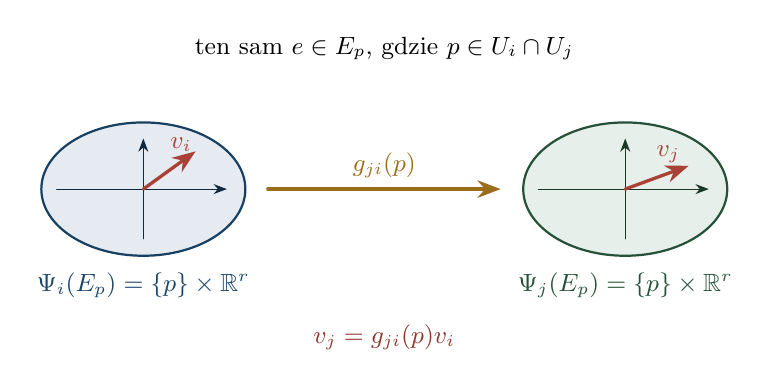
\begin{tikzpicture}[>=Stealth,scale=1.02,line cap=round]
\node[font=\small] at (0,1.75) {ten sam $e\in E_p$, gdzie $p\in U_i\cap U_j$};
\fill[manifoldblue!12] (-3,0) ellipse (1.27 and .83);
\draw[manifoldblue!70!black,thick] (-3,0) ellipse (1.27 and .83);
\draw[->,manifoldblue!45!black,thin] (-4.08,0)--(-1.96,0);
\draw[->,manifoldblue!45!black,thin] (-3,-.62)--(-3,.63);
\draw[->,manifoldred,very thick] (-3,0)--(-2.35,.47)
 node[pos=.72,above,font=\small] {$v_i$};
\fill[manifoldgreen!12] (3,0) ellipse (1.27 and .83);
\draw[manifoldgreen!65!black,thick] (3,0) ellipse (1.27 and .83);
\draw[->,manifoldgreen!45!black,thin] (1.92,0)--(4.04,0);
\draw[->,manifoldgreen!45!black,thin] (3,-.62)--(3,.63);
\draw[->,manifoldred,very thick] (3,0)--(3.79,.29)
 node[pos=.68,above,font=\small] {$v_j$};
\draw[->,very thick,manifoldgold!75!black] (-1.45,0)--(1.45,0)
 node[midway,above,font=\small] {$g_{ji}(p)$};
\node[font=\small,manifoldblue!75!black] at (-3,-1.2)
 {$\Psi_i(E_p)=\{p\}\times\R^r$};
\node[font=\small,manifoldgreen!65!black] at (3,-1.2)
 {$\Psi_j(E_p)=\{p\}\times\R^r$};
\node[font=\small\bfseries,manifoldred!85!black] at (0,-1.85)
 {$v_j=g_{ji}(p)v_i$};
\end{tikzpicture}
\caption{Dwie trywializacje tego samego włókna $E_p$. Wektor $e$ ma współrzędne $v_i$ i $v_j$, związane macierzą przejścia $g_{ji}(p)$.}
\end{figure}

\begin{uwaga}[Grupa strukturalna]
Wybór gładkich ramek lokalnych, równoważny wyborowi trywializacji
na mocy Stwierdzenia~\ref{prop:ramka-trywializacja},
daje funkcje przejścia o wartościach w
$\mathrm{GL}(r,\R)$; jest to
naturalna grupa strukturalna wiązki rzędu $r$. Jeżeli można dobrać
trywializacje tak, aby wszystkie macierze przejścia należały do podgrupy
$G\subseteq\mathrm{GL}(r,\R)$, mówimy o redukcji grupy strukturalnej do $G$.
Na przykład lokalne bazy ortonormalne wiązki z gładkim iloczynem
skalarnym we włóknach mają macierze przejścia w $\mathrm{O}(r)$.
W modelu wstęgi Möbiusa utożsamienie końców przedziału
zmienia znak współrzędnej włóknowej.
\end{uwaga}


\begin{przyklad}[Sekcje w zapisie lokalnym]
Niech $\pi:E\to M$ będzie wiązką wektorową rzędu $r$
z lokalnymi trywializacjami
$\Psi_i:E|_{U_i}\to U_i\times\R^r$ i funkcjami przejścia
$g_{ji}$.

Jeżeli $s:M\to E$ jest sekcją, to dla każdego $p\in U_i$
mamy $s(p)\in E_p$, a zatem $\Psi_i(s(p))=(p,s_i(p))$,
gdzie $s_i:U_i\to\R^r$ jest gładkim odwzorowaniem,
zwanym \emph{lokalnym zapisem sekcji} w trywializacji
$\Psi_i$.

Na przecięciu $U_i\cap U_j$ otrzymujemy
\[
\begin{aligned}
(p,s_j(p))
&=\Psi_j(s(p))\\
&=(\Psi_j\circ\Psi_i^{-1})(p,s_i(p))\\
&=(p,g_{ji}(p)s_i(p)),
\end{aligned}
\]
skąd $s_j(p)=g_{ji}(p)s_i(p)$.

Odwrotnie, jeżeli rodzina gładkich odwzorowań
$s_i:U_i\to\R^r$ spełnia powyższe warunki zgodności,
to wzór $s(p)=\Psi_i^{-1}(p,s_i(p)),\ p\in U_i$,
określa globalną sekcję wiązki $E$.
Istotnie, na przecięciu $U_i\cap U_j$ mamy
\[
\begin{aligned}
\Psi_j^{-1}(p,s_j(p))
&=\Psi_j^{-1}(p,g_{ji}(p)s_i(p))\\
&=\Psi_i^{-1}(p,s_i(p)),
\end{aligned}
\]
więc definicja nie zależy od wyboru indeksu.
Gładkość sekcji wynika z gładkości jej lokalnych
zapisów.

W szczególności, dla wiązki skonstruowanej przez
sklejanie z funkcji przejścia otrzymujemy $s(p)=[p,s_i(p)]_i$.

Rozważmy teraz wstęgę Möbiusa jako wiązkę liniową
nad okręgiem $S^1$. Możemy przedstawić ją jako
przestrzeń ilorazową $E=([0,2\pi]\times\R)/\sim$,
gdzie utożsamiamy $(0,v)\sim(2\pi,-v)$.
Rzutowanie na bazę jest dane wzorem $\pi([\theta,v])=e^{i\theta}$.

Sekcję opisujemy w tych współrzędnych za pomocą
funkcji $f:[0,2\pi]\to\R$, przypisując punktowi
$e^{i\theta}$ klasę $[\theta,f(\theta)]$.
Aby otrzymać dobrze określoną sekcję ciągłą,
funkcja $f$ musi być ciągła i spełniać $f(2\pi)=-f(0)$.
Dla sekcji gładkiej funkcja $f$ musi być gładka na domkniętym
przedziale i spełniać warunki zgodności wszystkich pochodnych
na utożsamianych końcach: $f^{(k)}(2\pi)=-f^{(k)}(0), \ k=0,1,2,\ldots$.

Pokażemy, że każda ciągła sekcja wstęgi Möbiusa
ma miejsce zerowe. Jeżeli $f(0)=0$, to teza
jest natychmiastowa. W przeciwnym razie
$f(2\pi)=-f(0)$ ma znak przeciwny do $f(0)$,
więc z twierdzenia o wartości pośredniej istnieje
$\theta_0\in(0,2\pi)$ takie, że $f(\theta_0)=0$.
Oznacza to, że $s(e^{i\theta_0})=0_{e^{i\theta_0}}$.

W szczególności wstęga Möbiusa nie posiada
globalnej sekcji nigdzie niezerowej, co stanowi
kolejny dowód jej nietrywialności jako wiązki
liniowej.
\end{przyklad}


\begin{definicja}[Suma i wiązka dualna]
\index{suma i wiazka dualna@Suma i wiązka dualna}
Dla wiązek $E,F$ nad tą samą bazą definiujemy włókna
$(E\oplus F)_p=E_p\oplus F_p$ oraz
$(E^*)_p=\mathrm{Hom}(E_p,\R)$. Przy macierzach przejścia $g_{ji}$
i $h_{ji}$ odpowiednie macierze to $g_{ji}\oplus h_{ji},\ (g_{ji}^{-1})^{\mathsf T}$.
Ostatni wzór wymusza zachowanie wartości funkcjonału:
jeżeli $v_j=g_{ji}v_i$ oraz $\xi_i(v_i)=\xi_j(v_j)$, to
$\xi_j=(g_{ji}^{-1})^{\mathsf T}\xi_i$. Obie rodziny spełniają
warunek kocyklu, więc twierdzenie o sklejaniu tworzy z nich wiązki.
\end{definicja}



\section{Różniczka, immersje, submersje i zanurzenia}

\begin{definicja}
Niech $F\colon M\to N$ będzie odwzorowaniem gładkim, $p\in M$. \emph{Różniczką} $F$ w
punkcie $p$ nazywamy odwzorowanie liniowe $dF_p\colon T_pM\to T_{F(p)}N$ zdefiniowane (w
języku derywacji) wzorem $(dF_p\,v)(g):=v(g\circ F), \ v\in T_pM,\ g\in C^\infty(N)$.

Równoważnie, jeśli $v=\gamma'(0)$ dla gładkiej krzywej
$\gamma\colon(-\varepsilon,\varepsilon)\to M$ z $\gamma(0)=p$, to $dF_p(v)=(F\circ\gamma)'(0)\in T_{F(p)}N$.
Istotnie, obie strony działają na $g\in C^\infty(N)$ jako
$(g\circ F\circ\gamma)'(0)=v(g\circ F)$. 
\end{definicja}

Jeśli krzywe $\gamma_1$ i
$\gamma_2$ mają tę samą prędkość $v$ w $p$, to dla każdego takiego $g$
obie prędkości $(F\circ\gamma_i)'(0)$ przyjmują na $g$ tę samą wartość
$v(g\circ F)$. Wektory styczne w $F(p)$ są derywacjami, więc są równe,
gdy działają jednakowo na wszystkie funkcje gładkie. Stąd wzór nie
zależy od wyboru krzywej reprezentującej $v$.
\begin{fakt}
$dF_pv$ jest istotnie derywacją w $F(p)$, a $dF_p$ jest odwzorowaniem liniowym.
\end{fakt}

\begin{proof}
Liniowość względem $g$: oczywista z liniowości $v$ i liniowości $g\mapsto g\circ F$.
Reguła Leibniza: $(dF_pv)(gh)=v((gh)\circ F)=v((g\circ F)(h\circ F))=(g\circ F)(p)\,
v(h\circ F)+(h\circ F)(p)\,v(g\circ F)=g(F(p))(dF_pv)(h)+h(F(p))(dF_pv)(g)$, na mocy reguły
Leibniza dla $v$ zastosowanej do $g\circ F,h\circ F\in C^\infty(M)$. Zatem $dF_pv\in
T_{F(p)}N$. Liniowość $dF_p$ względem $v$ jest natychmiastowa z liniowości $v\mapsto
v(g\circ F)$ w $v$, dla każdego ustalonego $g$.
\end{proof}

W Sekcji~\ref{sec:przestrzen-kostyczna} różniczkę funkcji
$f\colon M\to\R$ opisaliśmy jako kowektor $df_p\in T_p^*M$.
Powyższa definicja daje natomiast różniczkę odwzorowania
$f$ o wartościach w $T_{f(p)}\R$. Poniższy dowód utożsamia
te dwa opisy i wyjaśnia znany wzór na $df_p$ w mapie.



\begin{twierdzenie}[Różniczka odwzorowania we współrzędnych]
\label{tw:rozniczka-odwzorowania-wspolrzedne}
Niech $F\colon M\to N$ będzie odwzorowaniem gładkim, gdzie
$\dim M=m$ i $\dim N=n$. Niech $(U,\varphi)$ będzie mapą
wokół $p$, o współrzędnych $(x^1,\ldots,x^m)$, a $(V,\psi)$
mapą wokół $F(p)$, o współrzędnych $(y^1,\ldots,y^n)$.
Zmniejszając w razie potrzeby $U$, zakładamy, że
$F(U)\subset V$, i oznaczamy
\[
\widehat F:=\psi\circ F\circ\varphi^{-1}
=(\widehat F^{\,1},\ldots,\widehat F^{\,n}).
\]
Wówczas dla każdego $v\in T_pM$ zachodzi
\[
dF_p(v)=
\sum_{j=1}^n\sum_{i=1}^m
\frac{\partial\widehat F^{\,j}}{\partial u^i}
\bigl(\varphi(p)\bigr)\,dx_p^i(v)
\left.\frac{\partial}{\partial y^j}\right|_{F(p)}.
\]
W szczególności macierzą różniczki $dF_p$ w bazach
współrzędnościowych jest macierz Jacobiego
\[
[dF_p]=D\widehat F(\varphi(p))
=
\left[
\frac{\partial\widehat F^{\,j}}{\partial u^i}
\bigl(\varphi(p)\bigr)
\right]_{\substack{1\le j\le n\\1\le i\le m}}.
\]
\emph{Rzędem} odwzorowania $F$ w punkcie $p$ nazywamy
rząd $dF_p$, równy rzędowi powyższej macierzy.
\end{twierdzenie}

\begin{proof}
Z dualności baz współrzędnościowych mamy
\[
dx_p^i\left(
\left.\frac{\partial}{\partial x^j}\right|_p
\right)=\delta_j^i.
\]
Każdy wektor $v\in T_pM$ można zapisać jako
\[
v=\sum_{i=1}^m v^i
\left.\frac{\partial}{\partial x^i}\right|_p.
\]
Stosując $dx_p^j$ do obu stron, otrzymujemy
$v^j=dx_p^j(v)$, a zatem
\[
v=\sum_{i=1}^m dx_p^i(v)
\left.\frac{\partial}{\partial x^i}\right|_p.
\]

Niech $g$ będzie funkcją gładką określoną w otoczeniu
$F(p)$. Można ją przedłużyć funkcją odcinającą do funkcji
na $N$; wynik nie zależy od przedłużenia dzięki
Lematowi~\ref{lem:lokalnosc}. Dotyczy to również
lokalnych funkcji współrzędnych $y^j$ użytych poniżej.
Z definicji różniczki oraz powyższego rozkładu
wynika
\[
\begin{aligned}
(dF_p(v))(g)
&=v(g\circ F)\\
&=\sum_{i=1}^m dx_p^i(v)
\left.\frac{\partial}{\partial x^i}\right|_p(g\circ F)\\
&=\sum_{i=1}^m dx_p^i(v)
\frac{\partial(g\circ F\circ\varphi^{-1})}
{\partial u^i}\bigl(\varphi(p)\bigr).
\end{aligned}
\]

Aby wyznaczyć współrzędne wektora $dF_p(v)$,
stosujemy go do funkcji współrzędnych $y^j$.
Istotnie, z dualności baz w $T_{F(p)}N$ mamy
\[
w=\sum_{j=1}^n dy_{F(p)}^j(w)
\left.\frac{\partial}{\partial y^j}\right|_{F(p)},
\qquad
dy_{F(p)}^j(w)=w(y^j).
\]
Podstawiając $g=y^j$ i korzystając z równości
$\widehat F^{\,j}=y^j\circ F\circ\varphi^{-1}$,
otrzymujemy
\[
\begin{aligned}
dy_{F(p)}^j(dF_p(v))
&=(dF_p(v))(y^j)\\
&=\sum_{i=1}^m dx_p^i(v)
\frac{\partial\widehat F^{\,j}}{\partial u^i}
\bigl(\varphi(p)\bigr).
\end{aligned}
\]
Wstawiając te współczynniki do rozkładu wektora
$dF_p(v)$ w bazie współrzędnościowej, otrzymujemy
żądaną postać różniczki.

W szczególności, dla
$v=\partial/\partial x^i|_p$ mamy
\[
dF_p\left(
\left.\frac{\partial}{\partial x^i}\right|_p
\right)
=
\sum_{j=1}^n
\frac{\partial\widehat F^{\,j}}{\partial u^i}
\bigl(\varphi(p)\bigr)
\left.\frac{\partial}{\partial y^j}\right|_{F(p)}.
\]
Współczynniki przy wektorach bazy docelowej
tworzą kolejne kolumny macierzy $dF_p$,
czyli macierz Jacobiego $D\widehat F(\varphi(p))$.
\end{proof}

\begin{wniosek}[Różniczka funkcji we współrzędnych]
\label{tw:rozniczka-funkcji-wspolrzedne}
Niech $f\colon M\to\R$ będzie funkcją gładką,
a $(U,\varphi)$ mapą wokół $p$, o współrzędnych
$(x^1,\ldots,x^m)$. Oznaczmy
\[
\widehat f:=f\circ\varphi^{-1}.
\]
Po standardowym utożsamieniu $T_{f(p)}\R$ z $\R$
różniczka $df_p$ jest kowektorem i ma postać
\begin{equation}
\label{eq:df-wspolrzedne}
df_p=\sum_{i=1}^m
\frac{\partial f}{\partial x^i}(p)\,dx_p^i,
\qquad
\frac{\partial f}{\partial x^i}(p)
:=
\frac{\partial\widehat f}{\partial u^i}
\bigl(\varphi(p)\bigr).
\end{equation}
W szczególności, jeśli
$v=\sum_i v^i\partial/\partial x^i|_p$, to
\[
df_p(v)=\sum_{i=1}^m
v^i\frac{\partial f}{\partial x^i}(p).
\]
\end{wniosek}

\begin{proof}
Niech $t\colon\R\to\R$ będzie standardową
współrzędną, czyli $t(a)=a$. Każdy wektor
$w\in T_{f(p)}\R$ ma jednoznaczną postać
\[
w=a\left.\frac{\partial}{\partial t}\right|_{f(p)},
\qquad a\in\R.
\]
Standardowy izomorfizm $T_{f(p)}\R\cong\R$
przyporządkowuje temu wektorowi liczbę $a$.
Ponieważ
\[
\left.\frac{\partial}{\partial t}\right|_{f(p)}(t)=1,
\]
współczynnik ten możemy odczytać jako $a=w(t)$.
Zatem utożsamienie ma postać
\[
T_{f(p)}\R\longrightarrow\R,
\qquad w\longmapsto w(t).
\]

W szczególności różniczka odwzorowania
$f$, która pierwotnie przyjmuje wartości
w $T_{f(p)}\R$, po tym utożsamieniu spełnia
\[
df_p(v)=(df_p(v))(t)
=v(t\circ f)=v(f).
\]
Pierwsza równość oznacza tutaj zastosowanie
powyższego izomorfizmu, a druga wynika
z definicji różniczki odwzorowania.

Ponieważ lokalną reprezentacją $f$ względem
standardowej współrzędnej $t$ jest
$\widehat f=f\circ\varphi^{-1}$, poprzednie
twierdzenie daje
\[
df_p(v)=
\sum_{i=1}^m
\frac{\partial\widehat f}{\partial u^i}
\bigl(\varphi(p)\bigr)\,dx_p^i(v).
\]
Ponieważ równość zachodzi dla każdego
$v\in T_pM$, otrzymujemy wzór
\eqref{eq:df-wspolrzedne}.
\end{proof}

Na przykład dla $f(u,v)=u^2+uv$ na $\R^2$ mamy
$\partial_u f=2u+v$ i $\partial_v f=u$, więc
\[
 df_{(u,v)}=(2u+v)\,du_{(u,v)}+u\,dv_{(u,v)}.
\]
W punkcie $(1,2)$ dostajemy $df_{(1,2)}=4\,du_{(1,2)}+dv_{(1,2)}$;
na wektorze $a\,\partial_u|_{(1,2)}+b\,\partial_v|_{(1,2)}$
różniczka ma wartość $4a+b$.

\begin{twierdzenie}[Reguła łańcucha]
Jeśli $F\colon M\to N$ i $G\colon N\to P$ są gładkie, $p\in M$, to
$d(G\circ F)_p=dG_{F(p)}\circ dF_p\colon T_pM\to T_{G(F(p))}P$.
\end{twierdzenie}
\begin{proof}
Dla $v\in T_pM$ i $h\in C^\infty(P)$, z definicji różniczki:
\[
\big(d(G\circ F)_p\,v\big)(h)=v\big(h\circ(G\circ F)\big)=v\big((h\circ G)\circ F\big)=
(dF_pv)(h\circ G)=\big(dG_{F(p)}(dF_pv)\big)(h),
\]
gdzie w trzeciej równości zastosowaliśmy definicję $dF_p$ do $h\circ G\in C^\infty(N)$, a
w czwartej — definicję $dG_{F(p)}$ do $dF_pv\in T_{F(p)}N$. Zatem $d(G\circ F)_pv=
dG_{F(p)}(dF_pv)$ dla każdego $v$ — co dowodzi tezy.
\end{proof}


\begin{definicja}
Niech $F\colon M\to N$ będzie gładkie, $\dim M=m$, $\dim N=n$. Mówimy, że $F$ jest w
punkcie $p$ \emph{immersją}, jeśli $dF_p$ jest injektywne, oraz \emph{submersją}, jeśli
$dF_p$ jest surjektywne. $F$ jest immersją (submersją), jeśli jest nią w każdym punkcie
$p\in M$. \emph{Zanurzeniem} (ang.\ \emph{embedding}) nazywamy immersję $F\colon M\to N$,
która dodatkowo jest homeomorfizmem na obraz $F(M)$ (z topologią podprzestrzeni $N$).
\end{definicja}

Poniższy przykład pokazuje, że sama różnowartościowa immersja nie musi być zanurzeniem —
warunek ,,homeomorfizm na obraz'' jest istotnie mocniejszy.

\begin{przyklad}[Krzywa ósemkowa]\label{prz:osemka}
Niech $\beta\colon(-\pi,\pi)\to\R^2$, $\beta(t):=(\sin2t,\ \sin t)$.

\emph{$\beta$ jest immersją.} $\beta'(t)=(2\cos2t,\cos t)$. Gdyby $\beta'(t_0)=0$, to
$\cos t_0=0$ (więc $t_0=\pm\pi/2$) oraz $\cos2t_0=0$; ale $\cos(\pm\pi)=-1\neq0$ —
sprzeczność. Zatem $\beta'(t)\neq0$ dla wszystkich $t$, czyli $d\beta_t$ jest injektywne w
każdym punkcie.

\emph{$\beta$ jest różnowartościowa.} Przypuśćmy $\beta(t_1)=\beta(t_2)$, tzn.\ $\sin t_1=
\sin t_2=:s$ oraz $\sin2t_1=\sin2t_2$. Jeśli $s=0$: na $(-\pi,\pi)$ równość $\sin t=0$
zachodzi jedynie dla $t=0$, więc $t_1=t_2=0$. Jeśli $s\neq0$: korzystając z $\sin2t_i=
2\sin t_i\cos t_i=2s\cos t_i$, równość $\sin2t_1=\sin2t_2$ daje (dzieląc przez $2s\neq0$)
$\cos t_1=\cos t_2$. Zatem $\sin t_1=\sin t_2$ i $\cos t_1=\cos t_2$ jednocześnie — co
oznacza $t_1-t_2\in2\pi\Z$; ponieważ $t_1,t_2\in(-\pi,\pi)$, jedyna możliwość to $t_1=t_2$.
W obu przypadkach $\beta$ jest różnowartościowa.

\emph{$\beta$ nie jest zanurzeniem.} $\lim_{t\to\pi^-}\beta(t)=(\sin2\pi,\sin\pi)=(0,0)$
oraz $\lim_{t\to-\pi^+}\beta(t)=(0,0)$ — oba końce krzywej zbiegają do tego samego punktu
$(0,0)=\beta(0)$. Odwzorowanie odwrotne $\beta^{-1}$ nie jest więc ciągłe w $(0,0)$: dla
ciągu $t_k\to\pi^-$, $\beta(t_k)\to(0,0)=\beta(0)$, ale $\beta^{-1}(\beta(t_k))=t_k\to\pi
\neq0=\beta^{-1}(0,0)$. Zatem $\beta$ jest różnowartościową immersją, która nie jest
homeomorfizmem na obraz — nie jest zanurzeniem.
\end{przyklad}

\begin{figure}[h]
\centering
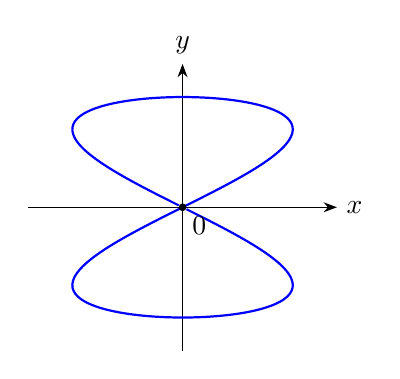
\begin{tikzpicture}[>=Stealth,scale=1.4]
\draw[->] (-1.4,0) -- (1.4,0) node[right]{$x$};
\draw[->] (0,-1.3) -- (0,1.3) node[above]{$y$};
\draw[thick,blue,domain=-179:179,samples=150,smooth]
plot ({sin(2*\x)},{sin(\x)});
\fill (0,0) circle (1pt) node[below right]{$0$};
\end{tikzpicture}
\caption{Krzywa ósemkowa $\beta(t)=(\sin2t,\sin t)$: różnowartościowa immersja, która nie
jest zanurzeniem — oba końce ($t\to\pm\pi$) zbiegają do początku układu współrzędnych.}
\label{fig:osemka}
\end{figure}


\begin{uwaga}[Nawinięcie niewymierne torusa]
Podobny, choć bardziej subtelny, przykład daje
\emph{nawinięcie niewymierne} torusa
$T^2=\R^2/\Z^2$. Rozważmy odwzorowanie $\gamma:\R\longrightarrow T^2, \ \gamma(t)=(t,\alpha t)+\Z^2$,
gdzie $\alpha\in\R\setminus\Q$.

Pokażemy, że $\gamma$ jest injektywną immersją,
która nie jest zanurzeniem, a jej obraz
jest gęsty w $T^2$.

\smallskip
\noindent\textbf{Injektywność i immersyjność.}
Jeżeli $\gamma(t)=\gamma(s)$, to $(t-s,\alpha(t-s))\in\Z^2$.
W szczególności $t-s\in\Z$ oraz
$\alpha(t-s)\in\Z$. Gdyby $t-s\ne0$,
otrzymalibyśmy $\alpha=\frac{\alpha(t-s)}{t-s}\in\Q$,
co przeczy niewymierności $\alpha$.
Zatem $t=s$, czyli $\gamma$ jest injektywna.

Ponieważ rzutowanie $\R^2\to T^2$ jest lokalnym
dyfeomorfizmem, różniczka $\gamma$ jest lokalnie
reprezentowana przez wektor $\gamma'(t)=(1,\alpha)\ne(0,0)$.
Ma więc rząd $1$ w każdym punkcie, co dowodzi,
że $\gamma$ jest immersją.

\smallskip
\noindent\textbf{Nieciągłość odwrotności na obraz.}
Wykażemy, że istnieje ciąg liczb całkowitych
dodatnich $q_N\to\infty$ taki, że $\gamma(q_N)\longrightarrow\gamma(0)$.

W tym celu ustalmy $N\ge1$ i podzielmy przedział
$[0,1)$ na $N$ rozłącznych przedziałów $I_j=\left[\frac{j}{N},\frac{j+1}{N}\right), \ j=0,\ldots,N-1$.
Każdy z nich ma długość $1/N$.

Rozważmy teraz $N+1$ liczb $\{0\alpha\},\{\alpha\},\{2\alpha\}, \ldots,\{N\alpha\}\in[0,1)$,
gdzie $\{x\}:=x-\lfloor x\rfloor$ oznacza
część ułamkową liczby $x$.

Ponieważ mamy $N+1$ liczb i tylko $N$
przedziałów, z zasady szufladkowej istnieją
indeksy $0\le k<l\le N$ takie, że
$\{k\alpha\}$ i $\{l\alpha\}$ należą do
tego samego przedziału $I_j$.

Wobec tego $|\{l\alpha\}-\{k\alpha\}|<\frac1N$.
Korzystając z definicji części ułamkowej,
otrzymujemy
\[
\left|
(l-k)\alpha-
\bigl(\lfloor l\alpha\rfloor
-\lfloor k\alpha\rfloor\bigr)
\right|<\frac1N.
\]
Oznaczając $q_N:=l-k,\ p_N:=\lfloor l\alpha\rfloor -\lfloor k\alpha\rfloor$,
dostajemy $1\le q_N\le N,\ p_N\in\Z, \ |q_N\alpha-p_N|<\frac1N$.

Pokażemy, że $q_N\to\infty$.
Gdyby tak nie było, istniałyby liczba
naturalna $K$ oraz nieskończenie wiele
indeksów $N$, dla których $q_N\le K$.
Ponieważ $\alpha$ jest niewymierna,
żadna z liczb $q\alpha$, $1\le q\le K$,
nie jest całkowita. Zatem $\delta_K:= \min_{1\le q\le K} \operatorname{dist}(q\alpha,\Z)>0$.
Jednak dla wspomnianych indeksów $N$ mamy $\delta_K \le |q_N\alpha-p_N| <\frac1N$,
co dla dostatecznie dużego $N$ prowadzi
do sprzeczności. Stąd $q_N\to\infty$.

Z drugiej strony, ponieważ $q_N,p_N\in\Z$,
w torusie zachodzi
\[
\begin{aligned}
\gamma(q_N)
&=(q_N,\alpha q_N)+\Z^2\\
&=(0,\alpha q_N-p_N)+\Z^2.
\end{aligned}
\]
Ponieważ $|\alpha q_N-p_N|<1/N$, otrzymujemy $\gamma(q_N)\longrightarrow(0,0)+\Z^2 =\gamma(0)$.

Przypuśćmy teraz, że odwrotność $\gamma^{-1}:\gamma(\R)\longrightarrow\R$
jest ciągła, przy czym $\gamma(\R)$
wyposażamy w topologię podprzestrzeni
odziedziczoną z $T^2$.

Z ciągłości $\gamma^{-1}$ w punkcie
$\gamma(0)$ oraz ze zbieżności
$\gamma(q_N)\to\gamma(0)$ wynikałoby
\[
q_N
=\gamma^{-1}(\gamma(q_N))
\longrightarrow
\gamma^{-1}(\gamma(0))=0.
\]
Jest to sprzeczne z $q_N\to\infty$.

Zatem $\gamma^{-1}$ nie jest ciągła,
a więc $\gamma$ nie jest homeomorfizmem
na swój obraz. W szczególności nie jest
zanurzeniem.

\smallskip
\noindent\textbf{Gęstość obrazu.}
Pokażemy jeszcze, że $\gamma(\R)$ jest
gęsty w $T^2$.

Najpierw udowodnimy, że zbiór $\{k\alpha+\Z:k\in\Z\}$
jest gęsty w okręgu $\R/\Z$.

Niech $\varepsilon\in(0,1)$.
Z wykazanego wyżej przybliżenia wynika,
że istnieją $q\in\N$ i $p\in\Z$ takie, że $0<|q\alpha-p|<\varepsilon$.
Oznaczmy $\delta:=q\alpha-p$ oraz
$d:=|\delta|$. Mamy więc $0<d<\varepsilon$.

Rozważmy punkty $0,d,2d,\ldots,\left\lfloor\frac1d\right\rfloor d$
w przedziale $[0,1]$.
Odległości między kolejnymi punktami
wynoszą $d$, natomiast odległość ostatniego
punktu od $1$ jest mniejsza niż $d$.
Zatem każdy punkt przedziału $[0,1]$
znajduje się w odległości mniejszej niż
$\varepsilon$ od jednego z tych punktów.

Ponadto każda wielokrotność $nd$ jest,
modulo $\Z$, całkowitą wielokrotnością
$\alpha$, gdyż $nd=n|q\alpha-p| \equiv \operatorname{sgn}(\delta)nq\alpha \pmod{\Z}$.
Wobec tego całkowite wielokrotności
$\alpha$ są $\varepsilon$-gęste
w $\R/\Z$. Ponieważ $\varepsilon>0$
było dowolne, otrzymujemy żądaną gęstość.

Niech teraz $(a,b)+\Z^2$ będzie dowolnym
punktem torusa. Z wykazanej gęstości
możemy dla dowolnego $\varepsilon>0$
wybrać $k\in\Z$ tak, aby $\operatorname{dist} \bigl(\alpha k-(b-\alpha a),\Z\bigr) <\varepsilon$.
Wtedy
\[
\begin{aligned}
\gamma(a+k)
&=(a+k,\alpha a+\alpha k)+\Z^2\\
&=(a,\alpha a+\alpha k)+\Z^2,
\end{aligned}
\]
a druga współrzędna tego punktu jest,
modulo $\Z$, odległa od $b$ o mniej
niż $\varepsilon$.

Ponieważ pierwsza współrzędna jest
dokładnie równa $a$ modulo $\Z$,
punkt $\gamma(a+k)$ może leżeć
dowolnie blisko $(a,b)+\Z^2$.
Stąd $\overline{\gamma(\R)}=T^2$.
\end{uwaga}


\subsection*{Twierdzenie o rzędzie stałym}

\begin{lemat}[Półciągłość rzędu z dołu]\label{lem:polciaglosc}
Niech $F\colon M\to N$ będzie gładkie. Zbiór $\{p\in M:\mathrm{rz}(dF_p)\geq r\}$ jest
otwarty w $M$, dla każdego $r$.
\end{lemat}
\begin{proof}
Warunek $\mathrm{rz}(dF_p)\geq r$ oznacza, w mapach lokalnych, że macierz Jacobiego $DF$ w
$\varphi(p)$ ma pewien minor stopnia $r$ różny od zera. Wyznacznik danego minora jest
funkcją ciągłą (wielomianem od wyrazów macierzy Jacobiego, gładkich funkcji punktu), więc
zbiór punktów, w których ten minor jest niezerowy, jest otwarty. Zbiór $\{\mathrm{rz}
(dF_p)\geq r\}$ jest sumą (po wszystkich wyborach minora stopnia $r$) takich zbiorów
otwartych, a więc otwarty.
\end{proof}

\begin{wniosek}\label{wn:stalyrzad}
Jeśli $F\colon M\to N$ jest immersją (submersją) w punkcie $p$, to $F$ jest immersją
(submersją) na pewnym otoczeniu $p$, o \emph{stałym} rzędzie na tym otoczeniu.
\end{wniosek}
\begin{proof}
Niech $m=\dim M$, $n=\dim N$. Jeśli $F$ jest immersją w $p$, $\mathrm{rz}(dF_p)=m$; ale
rząd $dF_q\colon\R^m\to\R^n$ jest zawsze $\leq m$, więc z Lematu~\ref{lem:polciaglosc}
($r=m$), $\{\mathrm{rz}(dF_q)\geq m\}=\{\mathrm{rz}(dF_q)=m\}$ jest otoczeniem otwartym
$p$, na którym $F$ ma stały rząd $m$. Przypadek submersji jest analogiczny z $r=n$.
\end{proof}

\begin{twierdzenie}[Twierdzenie o rzędzie stałym]
\label{tw:rzad-staly}
Niech $F\colon M\to N$
będzie odwzorowaniem gładkim o stałym rzędzie $k$ na pewnym otoczeniu
punktu $p\in M$, gdzie $\dim M=m, \ \dim N=n$.
Wówczas istnieją mapy $(U,\varphi) \ \text{oraz}\ (V,\psi)$
wokół odpowiednio $p$ i $F(p)$, takie że $\varphi(p)=0, \ \psi(F(p))=0, \ F(U)\subseteq V$,
oraz
\[
(\psi\circ F\circ\varphi^{-1})(u^1,\dots,u^m)
=
(u^1,\dots,u^k,0,\dots,0).
\]
\end{twierdzenie}
\begin{proof}
Wybierzmy najpierw dowolne mapy
\[
\varphi_0\colon U_0\to\varphi_0(U_0)\subset\R^m, \qquad \psi_0\colon V_0\to\psi_0(V_0)\subset\R^n
\]
wokół odpowiednio punktów $p$ i $F(p)$, takie że $\varphi_0(p)=0, \ \psi_0(F(p))=0$.
Po ewentualnym zmniejszeniu $U_0$ możemy założyć, że $F(U_0)\subseteq V_0$
oraz że $F$ ma stały rząd $k$ na całym $U_0$.

W tych mapach odwzorowanie $F$ jest reprezentowane przez gładkie
odwzorowanie
\[
\widehat F := \psi_0\circ F\circ\varphi_0^{-1} \colon \varphi_0(U_0)\longrightarrow\psi_0(V_0).
\]
Ponieważ $\varphi_0(p)=0 \ \text{oraz}\ \psi_0(F(p))=0$,
mamy $\widehat F(0)=0$.

Pokażmy najpierw, że $\widehat F$ ma ten sam rząd co $F$.
Niech $q\in U_0, \ u:=\varphi_0(q)$.
Z reguły łańcuchowej otrzymujemy
\[
D\widehat F_u = D(\psi_0)_{F(q)} \circ \dd F_q \circ D(\varphi_0^{-1})_u.
\]
Ponieważ $\varphi_0$ i $\psi_0$ są mapami, odwzorowania $D(\psi_0)_{F(q)} \ \text{oraz}\ D(\varphi_0^{-1})_u$
są izomorfizmami liniowymi. Złożenie odwzorowania liniowego
z izomorfizmami po lewej i prawej stronie nie zmienia jego rzędu,
a zatem $\operatorname{rz}(D\widehat F_u) = \operatorname{rz}(\dd F_q) = k$.
Odwzorowanie $\widehat F$ ma więc stały rząd $k$ na rozważanym
otoczeniu zera.

Dalszą część dowodu przeprowadzimy dla $\widehat F$ pomiędzy
otwartymi podzbiorami przestrzeni euklidesowych, a na końcu
przeniesiemy skonstruowane współrzędne z powrotem na rozmaitości.

\medskip
\emph{Przypadek $k=0$.}

Jeżeli $k=0$, to $D\widehat F_u=0$
dla każdego $u$ w dostatecznie małym otoczeniu zera.
Zmniejszając to otoczenie, możemy założyć, że jest ono wypukłe.

Dla ustalonego $u$ rozważmy krzywą $\gamma(t):=\widehat F(tu), \ 0\leq t\leq1$.
Z reguły łańcuchowej $\gamma'(t) = D\widehat F_{tu}(u) = 0$.
Krzywa $\gamma$ jest więc stała, a zatem $\widehat F(u) = \widehat F(0) = 0$.
Wobec tego $\widehat F(u)=(0,\dots,0)$,
czyli $\widehat F$ ma już żądaną postać normalną.

Po odpowiednim zmniejszeniu dziedzin możemy więc przyjąć $\varphi=\varphi_0, \ \psi=\psi_0$,
co kończy dowód w przypadku $k=0$.

Dalej zakładamy, że $k>0$.

\medskip
\emph{Krok 1: wybór odpowiednich współrzędnych i pierwszy
dyfeomorfizm lokalny.}

Ponieważ $\operatorname{rz}(D\widehat F(0))=k$,
istnieje niezerowy minor stopnia $k$ macierzy $D\widehat F(0)$.
Po odpowiednim przenumerowaniu współrzędnych w $\R^m$ oraz $\R^n$
możemy założyć, że jest to minor utworzony z pierwszych $k$
wierszy i pierwszych $k$ kolumn.

Formalnie takie przenumerowanie odpowiada złożeniu map
$\varphi_0$ i $\psi_0$ z odpowiednimi liniowymi izomorfizmami
będącymi permutacjami współrzędnych. Aby nie komplikować notacji,
otrzymane w ten sposób mapy nadal oznaczamy przez
$\varphi_0$ i $\psi_0$, a odpowiadającą im reprezentację $F$
przez $\widehat F$.

Piszemy $\widehat F = (\widehat F^1,\dots,\widehat F^n)$.
Macierz
\[
A := \left( \frac{\partial\widehat F^i}{\partial u^j}(0) \right)_{1\leq i,j\leq k}
\]
jest zatem odwracalna.

Definiujemy odwzorowanie $\Phi\colon\varphi_0(U_0)\to\R^m$
wzorem
\[
\Phi(u) := \bigl( \widehat F^1(u),\dots,\widehat F^k(u), u^{k+1},\dots,u^m \bigr).
\]
Macierz jego różniczki w zerze ma postać blokową
\[
D\Phi(0)
=
\begin{pmatrix}
A&B\\
0&I_{m-k}
\end{pmatrix}.
\]
Blok zerowy w lewym dolnym rogu pojawia się dlatego, że ostatnie
$m-k$ składowych $\Phi$ są funkcjami $u^{k+1},\dots,u^m$
i nie zależą od $u^1,\dots,u^k$.

Ponieważ macierz jest blokowo trójkątna, $\det D\Phi(0) = \det A\neq0$.
Na mocy twierdzenia o odwzorowaniu odwrotnym istnieje otwarte
otoczenie $W$ punktu $0$ takie, że $\Phi\colon W\longrightarrow\Phi(W)$
jest dyfeomorfizmem.

Po dalszym zmniejszeniu $U_0$ możemy zakładać, że $\varphi_0(U_0)\subseteq W$.

\medskip
\emph{Krok 2: przepisanie $\widehat F$ w nowych współrzędnych
dziedziny.}

Definiujemy $G := \widehat F\circ\Phi^{-1}$.
Niech $w=\Phi(u)$.
Z definicji $\Phi$ mamy $w^i=\widehat F^i(u), \ i=1,\dots,k$.
Ponieważ $G(w) = \widehat F(\Phi^{-1}(w)) = \widehat F(u)$,
otrzymujemy $G^i(w)=w^i, \ i=1,\dots,k$.

Dla pozostałych składowych wprowadzamy oznaczenie $h^i(w):=G^i(w), \ i=k+1,\dots,n$.
Wobec tego $G(w) = \bigl( w^1,\dots,w^k, h^{k+1}(w),\dots,h^n(w) \bigr)$.

\medskip
\emph{Krok 3: funkcje $h^i$ zależą tylko od
$w^1,\dots,w^k$.}

Ponieważ $G=\widehat F\circ\Phi^{-1}$,
a $\Phi^{-1}$ jest lokalnym dyfeomorfizmem, $G$ ma ten sam
stały rząd co $\widehat F$, czyli $\operatorname{rz}(DG(w))=k$.

Macierz różniczki $G$ ma postać
\[
DG(w)
=
\begin{pmatrix}
I_k&0\\
*&
\left(
\frac{\partial h^i}{\partial w^j}(w)
\right)_{\substack{i=k+1,\dots,n\\ j=k+1,\dots,m}}
\end{pmatrix}.
\]

Przypuśćmy, że dla pewnych $i_0>k, \ j_0>k$
oraz pewnego punktu $w_0$ zachodzi $\frac{\partial h^{i_0}}{\partial w^{j_0}}(w_0)\neq0$.
Rozważmy minor stopnia $k+1$ macierzy $DG(w_0)$ utworzony
z wierszy $1,\dots,k,i_0$
oraz kolumn $1,\dots,k,j_0$.
Odpowiadająca mu macierz ma postać
\[
\begin{pmatrix}
I_k&0\\
*&
\dfrac{\partial h^{i_0}}{\partial w^{j_0}}(w_0)
\end{pmatrix},
\]
więc jej wyznacznik wynosi $\frac{\partial h^{i_0}}{\partial w^{j_0}}(w_0)\neq0$.
Oznaczałoby to $\operatorname{rz}(DG(w_0))\geq k+1$,
co przeczy założeniu, że $G$ ma stały rząd $k$.

Zatem
\[
\frac{\partial h^i}{\partial w^j}=0
\qquad
\text{dla wszystkich }i>k,\ j>k.
\]

Zmniejszmy teraz dziedzinę $G$ tak, aby zawierała produkt
otwartych kul $A\times B \subset \R^k\times\R^{m-k}$
o środku $0$. Piszemy $w=(a,b), \ a=(w^1,\dots,w^k), \ b=(w^{k+1},\dots,w^m)$.
Dla $(a,b)\in A\times B$ oraz $i>k$ mamy
\begin{align*}
h^i(a,b)-h^i(a,0)
&=
\int_0^1
\frac{d}{dt}h^i(a,tb)\,dt\\
&=
\int_0^1
\sum_{j=k+1}^m
b^j
\frac{\partial h^i}{\partial w^j}(a,tb)\,dt\\
&=
0.
\end{align*}
Zatem $h^i(a,b)=h^i(a,0)$.
Każda funkcja $h^i$ zależy więc jedynie od pierwszych $k$
współrzędnych. Dalej będziemy pisać po prostu $h^i(w^1,\dots,w^k)$
zamiast $h^i(w^1,\dots,w^k,0,\dots,0)$.

W konsekwencji
\[
G(w) = \bigl( w^1,\dots,w^k, h^{k+1}(w^1,\dots,w^k), \dots, h^n(w^1,\dots,w^k) \bigr).
\]

\medskip
\emph{Krok 4: zmiana współrzędnych w przestrzeni docelowej.}

Na dostatecznie małym otwartym otoczeniu zera w $\R^n$
definiujemy
\[
\Psi(y^1,\dots,y^n)
:=
\bigl(
y^1,\dots,y^k,
y^{k+1}-h^{k+1}(y^1,\dots,y^k),
\dots,
y^n-h^n(y^1,\dots,y^k)
\bigr).
\]
Odwzorowanie to ma jawną odwrotność
\[
\Psi^{-1}(z^1,\dots,z^n)
=
\bigl(
z^1,\dots,z^k,
z^{k+1}+h^{k+1}(z^1,\dots,z^k),
\dots,
z^n+h^n(z^1,\dots,z^k)
\bigr).
\]
Bezpośrednie podstawienie pokazuje, że
\[
\Psi^{-1}\circ\Psi=\operatorname{id}
\qquad\text{oraz}\qquad
\Psi\circ\Psi^{-1}=\operatorname{id}.
\]
Odwzorowania $\Psi$ i $\Psi^{-1}$ są gładkie, zatem $\Psi$
jest dyfeomorfizmem swojego otwartego obszaru definicji na obraz.

Dla $w$ dostatecznie bliskiego $0$ mamy
\[
G(w) = \bigl( w^1,\dots,w^k, h^{k+1}(w^1,\dots,w^k), \dots, h^n(w^1,\dots,w^k) \bigr),
\]
a zatem
\begin{align*}
(\Psi\circ G)(w)
&=
\Psi\bigl(
w^1,\dots,w^k,
h^{k+1}(w^1,\dots,w^k),
\dots,
h^n(w^1,\dots,w^k)
\bigr)\\
&=
(w^1,\dots,w^k,0,\dots,0).
\end{align*}
Otrzymaliśmy więc w przestrzeniach euklidesowych postać normalną
\[
\Psi\circ\widehat F\circ\Phi^{-1}
= (w^1,\dots,w^k,0,\dots,0).
\]

\medskip
\emph{Krok 5: powrót do map na rozmaitościach.}

Pozostaje przełożyć skonstruowane powyżej zmiany współrzędnych
na nowe mapy rozmaitości $M$ i $N$.

Przypomnijmy, że początkowa reprezentacja $F$ miała postać $\widehat F = \psi_0\circ F\circ\varphi_0^{-1}$.
Odwzorowanie $\Phi$ jest zmianą współrzędnych po stronie dziedziny,
natomiast $\Psi$ jest zmianą współrzędnych po stronie przeciwdziedziny.

Definiujemy zatem nowe mapy przez
\[
\boxed{ \varphi:=\Phi\circ\varphi_0 }
\]
oraz
\[
\boxed{ \psi:=\Psi\circ\psi_0. }
\]
Po odpowiednim zmniejszeniu $U_0$ oraz $V_0$ są to mapy
\[
\varphi\colon U\to\varphi(U)\subset\R^m, \qquad \psi\colon V\to\psi(V)\subset\R^n
\]
wokół odpowiednio $p$ i $F(p)$.

Sprawdźmy najpierw położenie wyróżnionych punktów. Ponieważ $\varphi_0(p)=0$
oraz $\widehat F(0)=0$,
z definicji $\Phi$ otrzymujemy
\[
\Phi(0) = \bigl( \widehat F^1(0),\dots,\widehat F^k(0), 0,\dots,0 \bigr) = 0.
\]
Stąd $\varphi(p) = \Phi(\varphi_0(p)) = \Phi(0) = 0$.

Ponadto $G(0) = \widehat F(\Phi^{-1}(0)) = \widehat F(0) = 0$.
Ponieważ $G(0) = \bigl( 0,\dots,0, h^{k+1}(0),\dots,h^n(0) \bigr)$,
wynika stąd $h^{k+1}(0)=\cdots=h^n(0)=0$.
Z definicji $\Psi$ otrzymujemy więc $\Psi(0)=0$.
Wobec tego $\psi(F(p)) = \Psi(\psi_0(F(p))) = \Psi(0) = 0$.

Sprawdźmy teraz postać odwzorowania $F$ w nowych mapach.
Ponieważ $\varphi = \Phi\circ\varphi_0$,
mamy $\varphi^{-1} = \varphi_0^{-1}\circ\Phi^{-1}$.
Zatem
\begin{align*}
\psi\circ F\circ\varphi^{-1}
&=
(\Psi\circ\psi_0)
\circ F
\circ
(\varphi_0^{-1}\circ\Phi^{-1})\\
&=
\Psi
\circ
(\psi_0\circ F\circ\varphi_0^{-1})
\circ
\Phi^{-1}\\
&=
\Psi\circ\widehat F\circ\Phi^{-1}\\
&=
\Psi\circ G.
\end{align*}
Z Kroku~4 wynika więc, że
\[
(\psi\circ F\circ\varphi^{-1}) (u^1,\dots,u^m) = (u^1,\dots,u^k,0,\dots,0).
\]

Na końcu, zmniejszając w razie potrzeby otoczenie $U$ punktu $p$,
możemy zapewnić $F(U)\subseteq V$.
Otrzymaliśmy zatem mapy $(U,\varphi)$ i $(V,\psi)$ spełniające $\varphi(p)=0, \ \psi(F(p))=0, \ F(U)\subseteq V$,
oraz
\[
\boxed{ (\psi\circ F\circ\varphi^{-1})(u^1,\dots,u^m) = (u^1,\dots,u^k,0,\dots,0). }
\]
To kończy dowód.
\end{proof}

\begin{wniosek}[Postać lokalna immersji]\label{wn:immersja-lokalnie}
Jeśli $F\colon M\to N$ jest immersją w $p$ ($m\leq n$), to istnieją mapy wokół $p$, $F(p)$,
w których $F(u^1,\dots,u^m)=(u^1,\dots,u^m,0,\dots,0)$.
\end{wniosek}
\begin{proof}
Na mocy Wniosku~\ref{wn:stalyrzad}, $F$ ma stały rząd $m$ na otoczeniu $p$; stosujemy
Twierdzenie~\ref{tw:rzad-staly} z $k=m$.
\end{proof}

\begin{wniosek}[Postać lokalna submersji]\label{wn:submersja-lokalnie}
Jeśli $F\colon M\to N$ jest submersją w $p$ ($m\geq n$), to istnieją mapy wokół $p$, $F(p)$,
w których $F(u^1,\dots,u^m)=(u^1,\dots,u^n)$.
\end{wniosek}
\begin{proof}
Na mocy Wniosku~\ref{wn:stalyrzad}, $F$ ma stały rząd $n$ na otoczeniu $p$; stosujemy
Twierdzenie~\ref{tw:rzad-staly} z $k=n$ (teza redukuje się do $(u^1,\dots,u^n,0,\dots,0)\in
\R^n$, czyli po prostu $(u^1,\dots,u^n)$).
\end{proof}

\begin{przyklad}
Rzutowanie kanoniczne $\mathrm{pr}_1\colon M\times N\to M$ jest submersją: w mapach
produktowych, $\mathrm{pr}_1$ przyjmuje postać rzutowania liniowego $\R^m\times\R^n\to
\R^m$, którego różniczka (ono samo) jest surjektywna. Podobnie, rzutowanie wiązki
stycznej $\pi\colon TM\to M$ jest submersją — w mapach $\tilde\varphi_\alpha$ z Sekcji~\ref{sec:wiazki-wektorowe},
$\pi$ przyjmuje postać $(x,v)\mapsto x$.
\end{przyklad}
\section{Podrozmaitości}

Rozmaitość opisujemy za pomocą jej własnych map, bez wybierania
przestrzeni otaczającej. Podrozmaitość $S\subseteq M$ można badać
zarówno jako samodzielną rozmaitość, jak i jako część $M$:
podobnie powierzchnię Ziemi można opisywać mapami na samej powierzchni
albo jako powierzchnię w przestrzeni. Na przykład okrąg
$S^1\subset\R^2$ jest jednowymiarowy w swoich mapach, choć jego
punkty mają dwie współrzędne w $\R^2$. Poniższy warunek mapy
plasterkowej precyzuje tę sytuację: lokalnie $S$ zajmuje dokładnie
$\R^k\times\{0\}$ w przestrzeni współrzędnych $\R^n$ rozmaitości $M$.

\begin{definicja}
Niech $M$ będzie rozmaitością gładką wymiaru $n$, $S\subseteq M$ podzbiorem, $k\leq n$.
Mapa $(U,\varphi)$ na $M$ jest \emph{mapą plasterkową} (dostosowaną do $S$) rzędu $k$,
jeżeli
\[
\varphi(U\cap S)=\varphi(U)\cap(\R^k\times\{0\})\subseteq\R^k\times\R^{n-k}\cong\R^n.
\]
Mówimy, że $S$ jest \emph{podrozmaitością zanurzoną} wymiaru $k$ w $M$, jeśli każdy punkt
$p\in S$ posiada mapę plasterkową rzędu $k$ wokół $p$.
\end{definicja}

\begin{figure}[h]
\centering
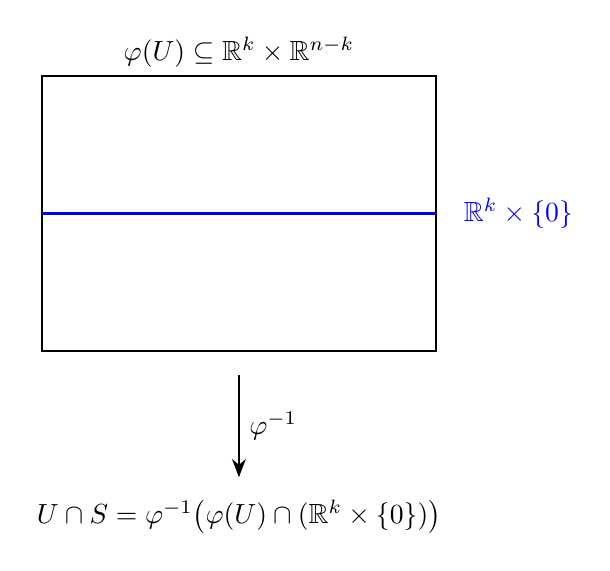
\begin{tikzpicture}[>=Stealth,scale=1]
\draw[thick] (0,0) rectangle (5,3.5);
\node at (2.5,3.8) {$\varphi(U)\subseteq\R^k\times\R^{n-k}$};
\draw[thick,blue] (0,1.75) -- (5,1.75);
\node[blue] at (6.05,1.75) {$\R^k\times\{0\}$};
\draw[->,thick] (2.5,-0.3) -- (2.5,-1.6) node[midway,right]{$\varphi^{-1}$};
\node at (2.5,-2.1) {$U\cap S=\varphi^{-1}\big(\varphi(U)\cap(\R^k\times\{0\})\big)$};
\end{tikzpicture}
\caption{Mapa plasterkowa: w mapie $\varphi$, przecięcie $U\cap S$ odpowiada dokładnie
przecięciu $\varphi(U)$ z podprzestrzenią $\R^k\times\{0\}$.}
\label{fig:plasterek}
\end{figure}

\begin{stwierdzenie}\label{stw:podrozm-struktura}
Jeśli $S\subseteq M$ jest podrozmaitością zanurzoną wymiaru $k$, to $S$ (z topologią
podprzestrzeni) jest rozmaitością topologiczną wymiaru $k$, posiadającą strukturę gładką,
względem której inkluzja $\iota\colon S\hookrightarrow M$ jest immersją; co więcej, $\iota$
jest zanurzeniem.
\end{stwierdzenie}
\begin{proof}
Wyposażamy $S$ w topologię podprzestrzeni. Ponieważ podprzestrzeń
przestrzeni Hausdorffa jest Hausdorffa, $S$ spełnia pierwszy warunek.
Jeśli $\mathcal B$ jest przeliczalną bazą $M$, to
$\{B\cap S:B\in\mathcal B\}$ jest przeliczalną bazą $S$:
dla otwartego $O\cap S$ i $p\in O\cap S$ znajdziemy
$B\in\mathcal B$ z $p\in B\subset O$, a wtedy
$p\in B\cap S\subset O\cap S$.

Ustalmy $p\in S$ i mapę plasterkową $(U,\varphi)$ przy $p$.
Ponieważ $U$ jest otwarte w $M$, zbiór $U_S=U\cap S$ jest otwarty
w $S$. Oznaczmy $W=\varphi(U)$, otwarty w $\R^n$.
Odwzorowanie $\varphi_S=\operatorname{pr}_1\circ\varphi|_{U_S}$
ma obraz $W_S=\{u\in\R^k:(u,0)\in W\}$, otwarty w $\R^k$ jako
przeciwobraz $W$ przez ciągłe zanurzenie $u\mapsto(u,0)$.
Odwrotność $u\mapsto\varphi^{-1}(u,0)$ jest ciągła; zatem
$\varphi_S:U_S\to W_S$ jest homeomorfizmem. To dowodzi lokalnej
euklidesowości $S$.

Niech teraz $(V,\psi)$ będzie drugą mapą plasterkową. Na
$\varphi_S(U\cap V\cap S)$ przejście ma wzór
\[
\psi_S\circ\varphi_S^{-1}(u)
=\operatorname{pr}_1\bigl((\psi\circ\varphi^{-1})(u,0)\bigr).
\]
Zanurzenie $u\mapsto(u,0)$, przejście $\psi\circ\varphi^{-1}$
i rzutowanie $\operatorname{pr}_1$ są gładkie, więc złożenie jest
gładkie. Zamieniając $\varphi$ i $\psi$, otrzymujemy gładką
odwrotność. Mapy $\varphi_S$ tworzą więc atlas gładki na $S$.

W mapach $\varphi_S$ i $\varphi$ inkluzja $\iota:S\to M$ ma postać
$u\mapsto(u,0)$, a jej różniczka wysyła $v$ na $(v,0)$ i jest
injektywna. Inkluzja jest więc immersją. Jako odwzorowanie
$S\to\iota(S)$ z \emph{topologią podprzestrzeni}, $\iota$ jest
homeomorfizmem już z wyboru topologii na $S$ (tożsamość na
zbiorze punktów). Zatem jest zanurzeniem.
\end{proof}



\begin{stwierdzenie}[Przestrzeń styczna do podrozmaitości]
\label{stw:styczna-podrozmaitosci}
\index{przestrzen styczna@Przestrzeń styczna!podrozmaitosci@podrozmaitości}
Niech $S\subseteq M$ będzie podrozmaitością zanurzoną wymiaru $k$
w rozmaitości $M$ wymiaru $n$, a $\iota\colon S\hookrightarrow M$
inkluzją. Dla $p\in S$ różniczka $d\iota_p$ utożsamia $T_pS$
z $k$-wymiarową podprzestrzenią $T_pM$. Jeśli mapa plasterkowa
przy $p$ ma współrzędne $(x^1,\ldots,x^k,y^1,\ldots,y^{n-k})$, to
\[
d\iota_p(T_pS)
=\operatorname{span}\left\{\left.\frac{\partial}{\partial x^i}\right|_p:
1\leq i\leq k\right\}
=\bigcap_{a=1}^{n-k}\ker(dy^a_p)\subseteq T_pM.
\]
Przy $k=0$ rozpiętość pustej rodziny oznacza $\{0\}$, a przy $k=n$
puste przecięcie oznacza $T_pM$.
Są to dokładnie prędkości $(\iota\circ\gamma)'(0)$ gładkich krzywych
$\gamma\colon(-\varepsilon,\varepsilon)\to S$ przechodzących przez $p$.
\end{stwierdzenie}
\begin{proof}
W mapie $\varphi_S$ na $S$ z dowodu
Stwierdzenia~\ref{stw:podrozm-struktura} inkluzja ma postać
$u\mapsto(u,0)$. Jej różniczka wysyła więc wektor o współrzędnych
$(a^1,\ldots,a^k)$ na $(a^1,\ldots,a^k,0,\ldots,0)$.
To daje pierwszy opis obrazu $d\iota_p$ i jego wymiar $k$.
Jeżeli $v\in T_pM$ ma współrzędne $(a^1,\ldots,a^k,b^1,\ldots,b^{n-k})$,
to $dy^a_p(v)=b^a$. Zatem wszystkie $dy^a_p(v)$ znikają dokładnie
wtedy, gdy $v$ należy do obrazu $d\iota_p$.

Każda krzywa w $S$ daje prędkość z tego obrazu na mocy reguły łańcucha.
Odwrotnie, dla dowolnego $(a^1,\ldots,a^k)$ krzywa
$\gamma(t)=\varphi_S^{-1}\bigl(\varphi_S(p)+t(a^1,\ldots,a^k)\bigr)$
jest określona dla dostatecznie małych $|t|$, leży w $S$ i jej prędkość
po inkluzji ma współrzędne $(a^1,\ldots,a^k,0,\ldots,0)$.
\end{proof}

\begin{przyklad}[Przestrzeń styczna do okręgu]
Niech $S^1=\{(x,y)\in\R^2:x^2+y^2=1\}$ i $p=(1,0)$.
Jest to jednowymiarowa podrozmaitość $\R^2$: dla
$f(x,y)=x^2+y^2$ różniczka $df_q(a,b)=2(q_1a+q_2b)$ jest niezerowa
w każdym $q=(q_1,q_2)\in S^1=f^{-1}(1)$, więc lokalna postać
submersji z Wniosku~\ref{wn:submersja-lokalnie} daje mapę plasterkową.
Jeśli $\eta(t)=(x(t),y(t))$ jest krzywą w $S^1$ przez $p$, to
różniczkowanie $x(t)^2+y(t)^2=1$ w $t=0$ daje $2x'(0)=0$.
Każda prędkość jest więc postaci $(0,b)$. Odwrotnie,
$\gamma_b(t)=(\cos bt,\sin bt)$ leży w $S^1$ i
$\gamma_b'(0)=(0,b)$. Stąd, przy $T_p\R^2\cong\R^2$,
\[
T_pS^1=\{(0,b):b\in\R\},\qquad
p+T_pS^1=\{(1,b):b\in\R\}.
\]
Pierwszy zbiór jest przestrzenią wektorów stycznych, a drugi ---
prostą styczną przechodzącą przez $p$ (rys.~\ref{fig:styczna-okrag}).
\end{przyklad}

\begin{figure}[ht]
\centering
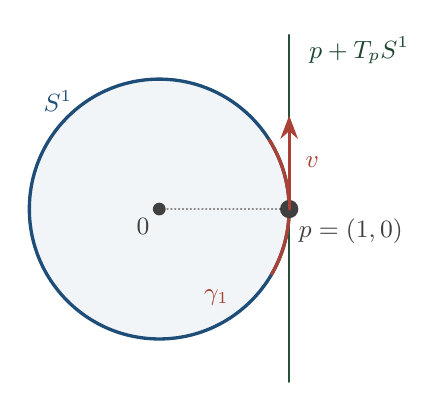
\begin{tikzpicture}[>=Stealth,scale=1.65,line cap=round,line join=round]
  \fill[manifoldblue!6] (0,0) circle (1);
  \draw[manifoldgreen!65!black,thick] (1,-1.33)--(1,1.34);
  \draw[black!45,densely dotted] (0,0)--(1,0);
  \draw[manifoldblue!85!black,very thick] (0,0) circle (1);
  \draw[manifoldred,very thick] plot[domain=-30:32,samples=30]
    ({cos(\x)},{sin(\x)});
  \fill[black!75] (0,0) circle (1.4pt) node[below left,font=\small] {$0$};
  \fill[black!75] (1,0) circle (2pt)
    node[below right,font=\small] {$p=(1,0)$};
  \draw[->,manifoldred,very thick] (1,0)--(1,.72)
    node[midway,right,font=\small,xshift=2pt] {$v$};
  \node[manifoldblue!85!black,font=\small] at (-.78,.83) {$S^1$};
  \node[manifoldred,font=\small] at (.44,-.68) {$\gamma_1$};
  \node[manifoldgreen!55!black,font=\small,anchor=west]
    at (1.08,1.22) {$p+T_pS^1$};
\end{tikzpicture}
\caption{Okrąg $S^1$ i jego prosta styczna w $p$. Czerwona krzywa
$\gamma_1$ biegnie po okręgu, a jej prędkość $v=\gamma_1'(0)=(0,1)$ wskazuje kierunek
styczny. Zielona prosta to przesunięcie przestrzeni wektorowej
$T_pS^1=\{(0,b):b\in\R\}$ do punktu $p$.}
\label{fig:styczna-okrag}
\end{figure}

\begin{przyklad}[Wiązka normalna jako wiązka ilorazowa]
Niech $S\subset M$ będzie podrozmaitością zanurzoną wymiaru $k$,
gdzie $\dim M=n$. Na mocy Stwierdzenia~\ref{stw:styczna-podrozmaitosci}
poprzez różniczkę inkluzji utożsamiamy
$T_pS$ z podprzestrzenią $T_pM$, a $TS$ traktujemy jako
podwiązkę wiązki ograniczonej $TM|_S$.

\emph{Wiązkę normalną} podrozmaitości $S$ definiujemy jako
wiązkę ilorazową $\nu S:=TM|_S/TS, \ \nu_pS:=T_pM/T_pS$.
Jej włókna są przestrzeniami wektorowymi wymiaru $n-k$.
Konstrukcja ta nie wymaga wyboru metryki ani dopełnienia
podprzestrzeni $T_pS$ w $T_pM$.

Pokażemy, że $\nu S$ jest wiązką wektorową rzędu $n-k$.
W mapie plasterkowej o współrzędnych $(x,y)$, gdzie
$x\in\R^k$ i $y\in\R^{n-k}$, podrozmaitość $S$ jest
opisana równaniem $y=0$. Wówczas
\[
T_pM=T_pS\oplus
\operatorname{span}\left\{
\left.\frac{\partial}{\partial y^1}\right|_p,
\ldots,
\left.\frac{\partial}{\partial y^{n-k}}\right|_p
\right\}.
\]
Każda klasa $[v]\in T_pM/T_pS$ ma zatem jednoznaczny
reprezentant w kierunkach $\partial/\partial y^a$,
co pozwala utożsamić lokalnie $\nu_pS$ z $\R^{n-k}$.

Sprawdźmy zmiany współrzędnych. Przejście między dwiema
mapami plasterkowymi ma postać $(x,y)\longmapsto(a(x,y),b(x,y))$,
przy czym $b(x,0)=0$. Różniczkując tę tożsamość
względem $x$, otrzymujemy $D_xb(x,0)=0$, więc
różniczka przejścia w punktach $S$ ma postać blokową
\[
\begin{pmatrix}
A&B\\
0&C
\end{pmatrix}.
\]
Cała macierz jest odwracalna, zatem kwadratowy blok
$C$ również jest odwracalny. Wektor o współrzędnych
$(u,v)\in\R^k\oplus\R^{n-k}$ przechodzi na $(u,v)\longmapsto(Au+Bv,Cv)$.
Ponieważ wektory styczne do $S$ odpowiadają
składowym $(u,0)$, klasa wektora w ilorazie
zmienia współrzędne według wzoru $[v]\longmapsto[Cv]$.
Zmiana ta zależy wyłącznie od składowej poprzecznej.

Macierze $C$ są gładkie i spełniają warunek kocyklu,
ponieważ różniczki przejść się składają, a iloczyn
macierzy blokowych zachowuje powyższą postać.
Twierdzenie o sklejaniu daje więc wiązkę wektorową
rzędu $n-k$ o włóknach $T_pM/T_pS$.

Otrzymujemy w ten sposób naturalny ciąg dokładny
wiązek wektorowych
\[
0\longrightarrow TS
\longrightarrow TM|_S
\longrightarrow \nu S
\longrightarrow 0.
\]
W szczególności konstrukcja wiązki normalnej jest
kanoniczna i nie wymaga żadnej dodatkowej struktury
geometrycznej na $M$.
\end{przyklad}


Poniższe twierdzenie i jego następstwa pokazują, w jaki sposób podrozmaitości powstają ,,w
praktyce'' — jako obrazy zanurzeń oraz jako przeciwobrazy wartości regularnych.

\begin{twierdzenie}[Twierdzenie o obrazie]\label{tw:obraz}
Jeśli $F\colon S\to M$ jest zanurzeniem ($\dim S=k\leq n=\dim M$), to $F(S)$ jest
podrozmaitością zanurzoną wymiaru $k$ w $M$, a $F\colon S\to F(S)$ (z topologią
podprzestrzeni) jest dyfeomorfizmem.
\end{twierdzenie}
\begin{proof}
Ustalmy $q=F(p_0)\in F(S)$. Ponieważ $F$ jest immersją w $p_0$, na mocy
Wniosku~\ref{wn:immersja-lokalnie} istnieją mapy $(U,\varphi)$ wokół $p_0$ w $S$ i
$(V,\psi)$ wokół $q$ w $M$, w których $F$ przyjmuje postać $u\mapsto(u,0)$.
Uzasadnijmy potrzebne dopasowanie dziedzin: wybieramy małe otwarte
kule $A\subset\R^k$, $B\subset\R^{n-k}$ o środku $0$, tak aby
$A\subset\varphi(U)$ i $A\times B\subset\psi(V)$.
Zastępujemy $U$ przez $\varphi^{-1}(A)$, a $V$ przez
$\psi^{-1}(A\times B)$. Wtedy rzeczywiście
$\psi(F(U))=A\times\{0\}=\psi(V)\cap(\R^k\times\{0\})$.
Zatem $(V,\psi)$ jest ,,prawie'' mapą
plasterkową dla $F(S)$, z tą różnicą, że warunek dotyczy $F(U)$, a nie od razu $F(S)\cap V$.

W tym miejscu wykorzystujemy założenie, że $F$ jest \emph{zanurzeniem}, nie tylko
różnowartościową immersją (por.\ Przykład~\ref{prz:osemka}): ponieważ $F\colon S\to F(S)$
jest homeomorfizmem na obraz, zbiór $F(U)$ jest otwarty w $F(S)$, tzn.\ $F(U)=F(S)\cap W$
dla pewnego otwartego $W\subseteq M$. Zastępując $V$ przez $V':=V\cap W$, otrzymujemy
$F(S)\cap V'=F(U)\cap V'$, a
\begin{align*}
\psi(F(S)\cap V')
 &=\psi(F(U)\cap V')\\
 &=\psi(F(U))\cap\psi(V')\\
 &=\big(\psi(V)\cap(\R^k\times\{0\})\big)\cap\psi(V')\\
 &=\psi(V')\cap(\R^k\times\{0\}).
\end{align*}
Zatem $(V',\psi|_{V'})$ jest mapą plasterkową rzędu $k$ dla $F(S)$ wokół $q$. Ponieważ
$q\in F(S)$ był dowolny, $F(S)$ jest podrozmaitością zanurzoną wymiaru $k$.

Wreszcie, $F\colon S\to F(S)$ jest bijekcją gładką (w mapach plasterkowych powyżej, $F$
przyjmuje postać identyczności), której odwrotność $F^{-1}\colon F(S)\to S$ jest gładka z
tego samego powodu. Zatem $F\colon S\to F(S)$ jest dyfeomorfizmem.
\end{proof}

\begin{definicja}
Niech $F\colon M\to N$ będzie gładkie, $q\in N$. Punkt $q$ jest \emph{wartością regularną}
$F$, jeśli dla każdego $p\in F^{-1}(q)$, $F$ jest submersją w $p$ (jeśli $F^{-1}(q)=
\emptyset$, $q$ jest — pusto — wartością regularną).
\end{definicja}

\begin{twierdzenie}[Twierdzenie o przeciwobrazie wartości regularnej]\label{tw:przeciwobraz}
Niech $F\colon M\to N$ będzie gładkie, $\dim M=m$, $\dim N=n$, i niech $q\in N$ będzie
wartością regularną $F$ z $F^{-1}(q)\neq\emptyset$. Wówczas $F^{-1}(q)$ jest
podrozmaitością zanurzoną wymiaru $m-n$ w $M$, a dla każdego $p\in F^{-1}(q)$,
$T_p\big(F^{-1}(q)\big)=\ker(dF_p)\subseteq T_pM$.
\end{twierdzenie}
\begin{proof}
Niech $p\in F^{-1}(q)$. Ponieważ $F$ jest submersją w $p$, na mocy
Wniosku~\ref{wn:submersja-lokalnie} istnieją mapy $(U,\varphi)$ wokół $p$ ($\varphi(p)=0$)
i $(V,\psi)$ wokół $q$ ($\psi(q)=0$), w których $F$ przyjmuje postać $\psi\circ F\circ
\varphi^{-1}(u^1,\dots,u^m)=(u^1,\dots,u^n)$. W tych mapach,
\[
\varphi(U\cap F^{-1}(q))=\{u\in\varphi(U):(u^1,\dots,u^n)=0\}=\varphi(U)\cap(\{0\}\times
\R^{m-n}).
\]
Po przenumerowaniu współrzędnych w $\R^m$ (zamiana miejscami pierwszych $n$ z pozostałymi
$m-n$), $(U,\varphi)$ staje się mapą plasterkową rzędu $m-n$ dla $F^{-1}(q)$ wokół $p$.
Ponieważ $p\in F^{-1}(q)$ był dowolny, $F^{-1}(q)$ jest podrozmaitością zanurzoną wymiaru
$m-n$.

W drugiej części niech $\iota\colon F^{-1}(q)\hookrightarrow M$
będzie inkluzją. Jest ona immersją na mocy
Stwierdzenia~\ref{stw:podrozm-struktura}. Ponieważ $F\circ\iota$ jest
odwzorowaniem stale równym $q$, jego różniczka znika: $dF_p\circ d\iota_p=0$ (reguła
łańcucha). Zatem $d\iota_p(T_pF^{-1}(q))\subseteq\ker(dF_p)$; utożsamiając (poprzez
injektywną różniczkę $d\iota_p$) $T_pF^{-1}(q)$ z jego obrazem w $T_pM$, mamy $T_pF^{-1}(q)
\subseteq\ker(dF_p)$. Z rachunku wymiarów: $\dim T_pF^{-1}(q)=m-n$ (z pierwszej części
dowodu), a $\dim\ker(dF_p)=m-\mathrm{rz}(dF_p)=m-n$ (bo $dF_p$ jest surjektywne na $T_qN$
wymiaru $n$, z definicji submersji). Zatem obie podprzestrzenie $T_pM$ mają ten sam,
skończony wymiar $m-n$, a jedna zawiera się w drugiej — więc są równe.
\end{proof}

\begin{wniosek}[Twierdzenie o poziomicy]
Jeśli $\dim M=n$, $f\colon M\to\R$ jest gładka, $c\in\R$ jest wartością regularną $f$ (tzn.\
$df_p\neq0$ dla każdego $p\in f^{-1}(c)$) i $f^{-1}(c)\neq\emptyset$, to $f^{-1}(c)$ jest
podrozmaitością zanurzoną wymiaru $n-1$ w $M$ (,,hiperpowierzchnią''), z $T_pf^{-1}(c)=
\ker(df_p)$.
\end{wniosek}
\begin{proof}
Szczególny przypadek Twierdzenia~\ref{tw:przeciwobraz} z $N=\R$: submersywność $f$ w
$p\in f^{-1}(c)$ to dokładnie warunek $df_p\neq0$.
\end{proof}

\begin{stwierdzenie}[Przestrzeń styczna i wektory normalne w $\R^m$]
\label{stw:styczna-normalne-euklidesowe}
Niech $S\subseteq\R^m$ będzie podrozmaitością zanurzoną wymiaru
$k<m$, a $p\in S$. Utożsamiajmy $T_pS$ z obrazem różniczki inkluzji
w $T_p\R^m\cong\R^m$. Załóżmy, że na otwartym otoczeniu $U$ punktu $p$
podrozmaitość jest opisana równaniami
\[
S\cap U=\{x\in U:f_1(x)=\cdots=f_{m-k}(x)=0\},
\]
gdzie $f_j\colon U\to\R$ są gładkie, a ich różniczki
$df_{1,q},\ldots,df_{m-k,q}$ są liniowo niezależne w każdym
$q\in S\cap U$. Wówczas
\[
T_pS=\bigcap_{j=1}^{m-k}\ker df_{j,p}
=\left(\operatorname{span}\{\nabla f_1(p),\ldots,
\nabla f_{m-k}(p)\}\right)^\perp\subseteq\R^m,
\]
gdzie $\nabla f_j(p)=
(\partial_1f_j(p),\ldots,\partial_mf_j(p))$ jest wektorem
współczynników różniczki względem standardowych współrzędnych.
Każda podrozmaitość zanurzona w $\R^m$ ma lokalnie taki opis:
funkcjami $f_j$ mogą być współrzędne poprzeczne mapy plasterkowej.
\end{stwierdzenie}
\begin{proof}
Odwzorowanie $F=(f_1,\ldots,f_{m-k})\colon U\to\R^{m-k}$
ma surjektywną różniczkę w każdym punkcie $S\cap U$,
bo jej składowe $df_{j,q}$ są liniowo niezależne. Zero jest więc
wartością regularną $F$. Z Twierdzenia~\ref{tw:przeciwobraz}
otrzymujemy $T_pS=\ker dF_p=\bigcap_j\ker df_{j,p}$.
W standardowym iloczynie skalarnym
$df_{j,p}(v)=\sum_{\ell=1}^m\partial_\ell f_j(p)v^\ell
=\langle\nabla f_j(p),v\rangle$.
Znikanie wszystkich tych iloczynów jest dokładnie prostopadłością
do rozpiętości wektorów $\nabla f_j(p)$.

W mapie plasterkowej $\varphi=(x^1,\ldots,x^k,y^1,\ldots,y^{m-k})$
można wybrać $f_j=y^j$: warunek $S\cap U=\{y=0\}$ jest częścią
definicji tej mapy, a różniczka $(y^1,\ldots,y^{m-k})$ jest
surjektywna, bo stanowi złożenie izomorfizmu $d\varphi_q$
z rzutowaniem na ostatnie $m-k$ współrzędnych.
\end{proof}

\begin{przyklad}
Niech $f\colon\R^{n+1}\to\R$, $f(x)=\|x\|^2$. Wtedy $df_x(v)=2\langle x,v\rangle$, niezerowe
dla $x\neq0$. Ponieważ $S^n=f^{-1}(1)$ i $0\notin f^{-1}(1)$, $1$ jest wartością regularną
— na mocy Wniosku powyżej, $S^n$ jest podrozmaitością zanurzoną wymiaru $n$ w $\R^{n+1}$
(zgodnie z tym, co wiedzieliśmy już z Przykładu~\ref{prz:sfera}; twierdzenie o poziomicy
daje jednak krótszy dowód gładkości struktury na $S^n$, choć nie podaje jawnych map).
\end{przyklad}

\begin{przyklad}[Grupa ortogonalna]
Niech $F\colon M_n(\R)\to\mathrm{Sym}(n)$, $F(A):=A^TA$, gdzie $\mathrm{Sym}(n)\cong
\R^{n(n+1)/2}$ oznacza przestrzeń macierzy symetrycznych. Dla $H\in T_AM_n(\R)\cong M_n(\R)$
stosujemy definicję różniczki przez krzywe do $\gamma(t)=A+tH$ w $M_n(\R)$:
\[
dF_A(H)=(F\circ\gamma)'(0)=\frac{d}{dt}\Big|_{t=0}(A+tH)^T(A+tH)=A^TH+H^TA.
\]
Dla $A\in\mathrm{O}(n):=F^{-1}(I)=\{A:A^TA=I\}$, $dF_A$ jest surjektywne na
$\mathrm{Sym}(n)$: dla symetrycznej $S$, kładąc $H:=\tfrac12AS$,
\[
dF_A(H)=A^T\big(\tfrac12AS\big)+\big(\tfrac12AS\big)^TA=\tfrac12(A^TA)S+\tfrac12S^TA^TA=
\tfrac12S+\tfrac12S=S
\]
(korzystając z $A^TA=I$, $S^T=S$). Zatem $I$ jest wartością regularną $F$, więc
$\mathrm{O}(n)=F^{-1}(I)$ jest podrozmaitością zanurzoną $M_n(\R)\cong\R^{n^2}$ wymiaru
$n^2-n(n+1)/2=n(n-1)/2$. Co więcej, $T_I\mathrm{O}(n)=\ker(dF_I)=\{H:H+H^T=0\}=:
\mathfrak{so}(n)$ — przestrzeń macierzy antysymetrycznych, wymiaru $n(n-1)/2$ (zgodnie z
powyższym rachunkiem wymiaru).
\end{przyklad}

\begin{uwaga}
Powyższy przykład jest pierwszym spotkaniem z fundamentalnym zjawiskiem: $\mathrm{O}(n)$
jest nie tylko rozmaitością, ale i grupą (względem mnożenia macierzy), w której mnożenie i
branie odwrotności są gładkie — tzw.\ \emph{grupą Liego} — a $T_I\mathrm{O}(n)=
\mathfrak{so}(n)$ jest jej \emph{algebrą Liego}.
\end{uwaga}

\begin{przyklad}[Torus jako regularna poziomica]
Niech $R>r>0$, $\rho=\sqrt{x^2+y^2}$ oraz
$\Omega=\{(x,y,z)\in\R^3:\rho>0\}$. Na tym otwartym zbiorze
$f(x,y,z)=(\rho-R)^2+z^2$ jest gładka. Poziom $f=r^2$
leży w $\Omega$, gdyż $|\rho-R|\leq r<R$ daje $\rho\geq R-r>0$.
Różniczka w punkcie $\Omega$ ma postać
\[
df=2(\rho-R)\left(\frac{x}{\rho}\,dx+
\frac{y}{\rho}\,dy\right)+2z\,dz.
\]
Jeżeli $df=0$, to $z=0$ oraz $\rho=R$: ponieważ $(x,y)\ne(0,0)$,
nie mogą jednocześnie znikać współczynniki przy $dx,dy$, chyba że
$\rho-R=0$. Lecz wtedy $f=0$, a więc taki punkt nie leży na
poziomie $r^2>0$. Zatem $r^2$ jest wartością regularną i torus
obrotowy $f^{-1}(r^2)$ jest gładką powierzchnią. Ponadto
$T_pT^2=\ker df_p$: wektor $(a,b,c)$ jest styczny wtedy i tylko
wtedy, gdy $(\rho-R)(xa+yb)/\rho+zc=0$.
\end{przyklad}

\par\smallskip
{\footnotesize\noindent\emph{Dalsza lektura:}
\href{https://www.ocw.mit.edu/courses/18-965-geometry-of-manifolds-fall-2004/34fad8f392208544e2b1e9794c33cbe7_lecture1.pdf}
{T.~S.~Mrowka, \emph{Geometry of Manifolds}, wykład~1},
definicje i przykłady rozmaitości;
\href{https://www.ocw.mit.edu/courses/18-965-geometry-of-manifolds-fall-2004/de18bf0029c583cacffb09810879bb54_lecture7.pdf}
{tenże, wykład~7}, wiązka styczna;
\href{https://pi.math.cornell.edu/~hatcher/VBKT/VB.pdf}
{A.~Hatcher, \emph{Vector Bundles and K-Theory}, \S\,1.1},
wiązki wektorowe.\par}

\clearpage

\chapter{Pola wektorowe, przepływy i pochodna Liego}
\label{ch:pola}

\providecommand{\atlasref}[2]{#2}
\index{pole wektorowe}

W Rozdziale~\ref{ch:rozmaitosci} zbudowaliśmy przestrzenie styczne i wiązkę $TM$.
Teraz wybieramy wektor \emph{w każdym} punkcie, w sposób gładki.
Otrzymujemy pole wektorowe: jednocześnie operator
różniczkowy, kierunek ruchu i infinitezymalny generator lokalnych dyfeomorfizmów.
Z tego jednego pojęcia wynikają nawias Liego, krzywe całkowe, przepływy oraz
pochodna Liego.

Rozdział rozwija rachunek pól oraz geometrię ich przepływów: najpierw
rozwiązujemy równanie krzywej całkowej, a następnie badamy ruch
punktów i sposób przenoszenia funkcji oraz pól wektorowych.
Do dalszej topologii różniczkowej przydadzą się zwłaszcza prostowanie
pola, pola zależne od czasu oraz rozszerzanie izotopii.
Przez $M$ rozumiemy rozmaitość gładką w sensie Definicji~\ref{def:rozmaitosc-gladka},
bez brzegu, chyba że wyraźnie zaznaczono inaczej.
Wszystkie pola i odwzorowania są klasy $C^\infty$.
Uwagi o brzegu i końcach przedziału czasu rozumiemy
według Definicji~\ref{def:rozmaitosc-z-brzegiem-1}
i opisu przestrzeni stycznej w
Stwierdzeniu~\ref{prop:styczna-brzeg-1}.
Tak samo interpretujemy gładkie rodziny na domkniętym przedziale czasu.



\section{Pola wektorowe i derywacje globalne}
\label{sec:derywacje}

W Sekcji~\ref{sec:przestrzen-styczna} utożsamiliśmy wektor $v\in T_pM$ z
\emph{derywacją w punkcie} $v\colon C^\infty(M)\to\R$:
po zastosowaniu do funkcji otrzymujemy liczbę. Pole wybiera taki
wektor w każdym punkcie, a jego działanie na funkcję zwraca nową
funkcję. Rozróżnienie tych dwóch typów derywacji będzie istotne.

\begin{definicja}
\emph{Pole wektorowe} $X$ na $M$ to gładka sekcja wiązki stycznej
$TM\to M$, czyli gładkie odwzorowanie $X\colon M\to TM$ spełniające
$X(p)\in T_pM$ dla każdego $p$. Przestrzeń pól oznaczamy $\X(M)=\Gamma(TM)$.
\end{definicja}

Wartość pola w ustalonym punkcie oznaczamy $X_p:=X(p)$.
Jest to jeden wektor styczny w $T_pM$; zapis $X_p(f)$ oznacza
działanie tego wektora jako derywacji w punkcie $p$ na funkcję $f$.
Na przykład wzór $X_{(u,v)}=(-v,u)$ na $\R^2$, po utożsamieniu
$T_{(u,v)}\R^2$ z $\R^2$, określa pole:
w każdym punkcie przypisuje wektor styczny zależny gładko od $(u,v)$.
Poza początkiem układu wektor jest styczny do okręgu o środku w zerze,
a w początku $X_{(0,0)}=0$.

W mapie $(U;x^1,\ldots,x^n)$ pole zapisuje się jednoznacznie jako
\begin{equation}\label{eq:lokalne-pole}
 X\big|_U=\sum_{i=1}^{n}X^i\frac{\partial}{\partial x^i},
 \qquad X^i\in C^\infty(U).
\end{equation}
Dokładniej, dla $p\in U$ jest to równość w $T_pM$:
$X_p=\sum_iX^i(p)\,\partial_{x^i}|_p$.
Lokalna trywializacja $TM$ z Rozdziału~\ref{ch:rozmaitosci}
pokazuje, że gładkość sekcji $X$ jest równoważna gładkości
wszystkich $X^i$ w każdej mapie. W drugą stronę gładkie współczynniki
na obszarach map określają jedno pole, jeżeli na przecięciach
opisują te same wektory styczne.

Geometrycznie $X_p$ wskazuje kierunek i prędkość w punkcie $p$.
Jeżeli $f\in C^\infty(M)$, czyli $f\colon M\to\R$,
opisuje na przykład temperaturę, to $X_p(f)$ jest chwilowym
tempem jej zmiany w kierunku wyznaczonym przez $X_p$.

Sprawdźmy tę interpretację na krzywej reprezentującej $X_p$.
W modelu z Sekcji~\ref{sec:przestrzen-styczna} każdy wektor
styczny jest reprezentowany przez klasę krzywych.
Wybierzmy mapę $(U,\varphi)$ wokół $p$, gdzie
$\varphi=(x^1,\ldots,x^n)$, i zapiszmy
$X_p=\sum_{i=1}^n X^i(p)\,\partial_{x^i}|_p$.
Na $\varphi(U)$ używamy standardowych współrzędnych
$u^1,\ldots,u^n$.
Oznaczmy $a=(X^1(p),\ldots,X^n(p))\in\R^n$ i rozważmy
krzywą $c(t)=\varphi(p)+ta$ w przestrzeni współrzędnych.
Ponieważ $\varphi(U)$ jest otwarty i $c(0)=\varphi(p)$,
istnieje $\varepsilon>0$ takie, że
$c((-\varepsilon,\varepsilon))\subset\varphi(U)$.
Możemy zatem zdefiniować
\[
\gamma\colon(-\varepsilon,\varepsilon)\to U,
\qquad
\gamma(t)=\varphi^{-1}\bigl(\varphi(p)+ta\bigr).
\]
Krzywa ta jest gładka i spełnia $\gamma(0)=p$ oraz
$(\varphi\circ\gamma)'(0)=a$, więc jej klasa $[\gamma]$
odpowiada wektorowi $X_p$ przy utożsamieniu
z rozdziału~1.

Pokażemy, że $X_p(f)$ jest pochodną funkcji $f$
wzdłuż skonstruowanej krzywej. Ponieważ
$\gamma=\varphi^{-1}\circ c$ i $\gamma(t)\in U$,
złożenie $f\circ\gamma$ jest dobrze określone oraz
$f\circ\gamma=(f\circ\varphi^{-1})\circ c$.
Stosując regułę łańcucha, otrzymujemy
\[
\begin{aligned}
\left.\frac{\dd}{\dd t}\right|_{t=0}f(\gamma(t))
&=D(f\circ\varphi^{-1})(\varphi(p))\cdot c'(0)\\
&=\sum_{i=1}^n X^i(p)
  \frac{\partial(f\circ\varphi^{-1})}{\partial u^i}
  (\varphi(p))
=X_p(f).
\end{aligned}
\]
Ostatnia równość wynika z definicji derywacji
współrzędnościowych. Rachunek obowiązuje dla każdej krzywej
o klasie $[\gamma]=X_p$: jej prędkość w mapie w chwili $t=0$
jest zawsze równa $a$. Niezależność tej klasy od wyboru mapy
ustaliliśmy w Sekcji~\ref{sec:przestrzen-styczna}.

Krzywa $\gamma$ reprezentuje zatem wektor w jednym
punkcie; jej dalszy przebieg nie wpływa na $X_p(f)$.
Nie musi być przy tym krzywą całkową pola $X$,
gdyż wymagamy jedynie zgodności jej wektora stycznego
z $X_p$ w chwili $t=0$.


\begin{definicja}
\emph{Derywacją} algebry $C^\infty(M)$ nazywamy $\R$-liniowe odwzorowanie
$D\colon C^\infty(M)\to C^\infty(M)$ spełniające regułę Leibniza
\[
 D(fg)=fD(g)+gD(f),\qquad f,g\in C^\infty(M).
\]
Zbiór takich derywacji oznaczamy $\operatorname{Der}_{\R}(C^\infty(M))$.
\end{definicja}

Warunek $\R$-liniowości oznacza liniowość względem stałych liczb.
Z reguły Leibniza wynika $D(1)=D(1\cdot1)=2D(1)$, więc $D(1)=0$
i $D(c)=0$ dla stałej $c$. Derywacja nie jest na ogół
$C^\infty(M)$-liniowa jako operator na funkcjach: jej działanie na
$hf$ zawiera dodatkowy składnik $fD(h)$.

Zacznijmy od pola $X$. Dla każdej funkcji $f\in C^\infty(M)$ określamy
\emph{funkcję} $D_X(f)$ przez
\[
 D_X(f)(p):=X_p(f),\qquad p\in M.
\]
W mapie $X_p=\sum_iX^i(p)\,\partial_i|_p$, więc
\[
 D_X(f)\big|_U=\sum_i X^i\partial_i f,
 \qquad D_X(f)(p)=\sum_iX^i(p)\,\partial_i f(p).
\]
W pierwszym wzorze $\partial_i f$ oznacza lokalną pochodną
$f\circ\varphi^{-1}$, przeniesioną z powrotem na $U$.
Suma gładkich funkcji jest gładka. Drugi wzór daje liczbę, bo
po ustaleniu $p$ współczynniki $X^i(p)$ są liczbami.
Punktowa reguła Leibniza dla $X_p$ daje
$D_X(fg)=fD_X(g)+gD_X(f)$ po sprawdzeniu równości w każdym punkcie.
Tak z pola otrzymujemy derywację globalną $D_X$.

W drugą stronę zacznijmy od \emph{dowolnej} derywacji globalnej $D$.
Dla ustalonego $p$ składamy ją z ewaluacją w $p$ i oznaczamy
\[
 v_p(f):=\bigl(D(f)\bigr)(p),\qquad
 C^\infty(M)\xrightarrow{\ D\ }C^\infty(M)
 \xrightarrow{\ \operatorname{ev}_p\ }\R.
\]
Funkcjonał $v_p$ jest $\R$-liniowy. Po ewaluacji globalnej
reguły Leibniza dostajemy \emph{punktową} regułę:
\[
 v_p(fg)=f(p)v_p(g)+g(p)v_p(f).
\]
Z definicji przestrzeni stycznej $v_p\in T_pM$; nie jest to już
operator o wartościach funkcyjnych. Lemat~\ref{lem:lokalnosc}
zapewnia, że $v_p(f)=D(f)(p)$ zależy tylko od kiełka $f$ w $p$.
Samo złożenie z ewaluacją daje na razie rodzinę wektorów;
jej gładkość trzeba jeszcze udowodnić.

\begin{twierdzenie}\label{thm:derywacje-pola}
Odwzorowanie
\[
 \X(M)\longrightarrow\operatorname{Der}_{\R}(C^\infty(M)),
 \qquad X\longmapsto D_X,\qquad D_X(f)(p)=X_p(f),
\]
jest izomorfizmem $C^\infty(M)$-modułów.
\end{twierdzenie}
\begin{proof}
Sprawdziliśmy wyżej, że $D_X$ jest derywacją, a dowolna
derywacja globalna $D$ wyznacza wektory $X_p(f):=D(f)(p)$.
Pozostaje pokazać, że $X\colon p\mapsto X_p$ jest gładką sekcją.

Ustalmy $p_0\in M$ i mapę $(U;x^1,\ldots,x^n)$ wokół $p_0$.
Wybierzmy otoczenie $V$ punktu $p_0$ o zwartym domknięciu zawartym w $U$
oraz funkcję odcinającą $\chi\in C^\infty(M)$, równą $1$ na
otoczeniu $\overline V$ i o nośniku zawartym w $U$.
Funkcja $\widetilde x^i$, zadana na $U$ przez $\chi x^i$ i równa
$0$ poza $U$, jest gładka na $M$. Na $V$ ma ten sam kiełek co $x^i$.
Z Twierdzenia~\ref{tw:baza-styczna} (po ewentualnym przesunięciu
początku współrzędnych) i lokalności derywacji punktowych
wynika, że dla $p\in V$
\[
 X_p=\sum_i a^i(p)\,\frac{\partial}{\partial x^i}\Big|_p,
 \qquad a^i(p)=X_p(\widetilde x^i)=D(\widetilde x^i)(p).
\]
Istotnie, działanie obu stron na $\widetilde x^j$ daje tę samą
liczbę $a^j(p)$, ponieważ
$\partial_{x^i}|_p(\widetilde x^j)=\delta_i^j$.
Każde $a^i=D(\widetilde x^i)|_V$ jest gładkie, gdyż $D$ przyjmuje
wartości w $C^\infty(M)$. Gładkość lokalnych współczynników
wokół każdego $p_0$ dowodzi gładkości $X$.

Dla każdego $f$ i $p$ mamy z konstrukcji
$D_X(f)(p)=X_p(f)=D(f)(p)$, zatem $D_X=D$.
Odwrotnie, jeśli zaczniemy od pola $X$, to ewaluacja $D_X$
w $p$ odzyskuje $X_p$ jako derywację punktową. Konstrukcje są więc
wzajemnie odwrotne. Dodawanie pól odpowiada dodawaniu derywacji,
a dla $h\in C^\infty(M)$ zachodzi
$D_{hX}(f)(p)=h(p)X_p(f)=(hD_X)(f)(p)$.
\end{proof}

Odtąd skracamy zapis $D_X(f)$ do $X(f)$; jest to funkcja na $M$,
podczas gdy $X_p(f)=X(f)(p)$ jest liczbą.

Na przykład na $\R$ operator $D(f)(x)=x^2f'(x)$ jest derywacją
globalną: $D(fg)(x)=x^2(f'(x)g(x)+f(x)g'(x))
=D(f)(x)g(x)+f(x)D(g)(x)$. Odpowiada mu pole
$X=x^2\partial_x$. W ustalonym punkcie $p$ jego wektor
$X_p=p^2\,\frac{\dd}{\dd x}\big|_p$ działa na funkcję przez
$X_p(f)=p^2f'(p)$; w szczególności $X_2(f)=4f'(2)$.
Współczynnik $x^2$ pola staje się liczbą $p^2$ po ustaleniu punktu.

\begin{uwaga}[Moduł pól i lokalne bazy]
Przestrzeń $\X(M)$ jest modułem nad pierścieniem funkcji:
$(hX)_p=h(p)X_p$. Po stronie derywacji mnożenie określa wzór
$(hD)(f)=hD(f)$; reguła Leibniza dla $hD$ wynika przez pomnożenie
obu stron reguły dla $D$ przez $h$.
Nie musi istnieć globalna baza modułu $\X(M)$ nad $C^\infty(M)$.
Na przykład $TS^2$ nie jest wiązką trywialną; nie da się wybrać
dwóch globalnych, wszędzie liniowo niezależnych pól na sferze.
Lokalne bazy $\partial_{x^1},\ldots,\partial_{x^n}$ zawsze istnieją.
Używamy tu klasycznego twierdzenia o nieistnieniu nigdzie
niezerowego pola na $S^2$; wynika ono również z późniejszego
Twierdzenia~\ref{thm:poincare-hopf-16} i $\chi(S^2)=2$.
\end{uwaga}

\begin{uwaga}[Przeniesienie pola przez mapę i zmiana współrzędnych]
Niech $(U,\varphi)$ będzie mapą rozmaitości $M$
o współrzędnych $x^1,\ldots,x^n$.
Ponieważ $\varphi\colon U\to\varphi(U)$ jest dyfeomorfizmem,
przenosi pole $X$ z $U$ na otwarty zbiór $\varphi(U)\subset\R^n$:
\begin{equation}\label{eq:pole-przeniesione-mapa}
\widehat X_\varphi(u)
:=(\dd\varphi)_{\varphi^{-1}(u)}X_{\varphi^{-1}(u)},
\qquad u\in\varphi(U).
\end{equation}
Piszemy $X_\varphi^i$ dla współczynników $X^i$
ze wzoru~\eqref{eq:lokalne-pole} w tej mapie;
indeks $\varphi$ odróżnia je od współczynników w innej mapie.
Jeśli $p=\varphi^{-1}(u)$ i
$X_p=\sum_iX_\varphi^i(p)\,\partial_{x^i}|_p$,
to współczynniki $\widehat X_\varphi(u)$ w standardowej bazie
$T_u\R^n$ wynoszą $X_\varphi^i(p)$.

W drugiej mapie $(V,\psi)$, o współrzędnych $y^1,\ldots,y^n$,
to samo pole ma na $U\cap V$ zapis
$X=\sum_jX_\psi^j\partial_{y^j}$.
Oznaczmy $G=\psi\circ\varphi^{-1}$.
Z reguły łańcucha dla $\psi=G\circ\varphi$ dostajemy
\[
\widehat X_\psi\bigl(G(u)\bigr)
=DG(u)\,\widehat X_\varphi(u),
\qquad u\in\varphi(U\cap V).
\]
Porównując $j$-te składowe, otrzymujemy regułę zmiany
współczynników pola:
\begin{equation}\label{eq:transformacja-wspolczynnikow-pola}
X_\psi^j(p)=\sum_i\frac{\partial y^j}{\partial x^i}(p)\,X_\varphi^i(p).
\end{equation}
Jest to ten sam rachunek co zmiana baz
z~\eqref{eq:transformacja-derywacji}.
Na przykład dla zmiany współrzędnej $y=2x$ na $\R$ pole
$X=a(x)\partial_x$ ma w nowej współrzędnej postać
$X=2a(y/2)\partial_y$.
\end{uwaga}

\begin{uwaga}[Od pola w przestrzeni otaczającej do współrzędnych]
Prześledźmy kolejność kroków, którą zastosujemy na okręgu i sferze.
Niech $M\subset\R^N$ będzie gładką podrozmaitością zanurzoną,
z inkluzją
$\iota\colon M\hookrightarrow\R^N$. Najpierw znamy pole $W$
na $\R^N$. Sprawdzamy, czy w punktach $p\in M$ jego wektor
$W_p\in T_p\R^N$ jest styczny do $M$, czyli należy do obrazu
$(\dd\iota)_p(T_pM)$. Dopiero wtedy możemy mówić o polu na samej
rozmaitości: ponieważ $(\dd\iota)_p$ jest injektywna
(Stwierdzenie~\ref{stw:styczna-podrozmaitosci}), istnieje
jedyny $X_p\in T_pM$ taki, że
\[
(\dd\iota)_pX_p=W_p.
\]
To są wektory w dwóch różnych przestrzeniach stycznych;
nie stosujemy $(\dd\varphi)_p$ bezpośrednio do $W_p$.
Gładkość $X$ wynika z gładkości $W$: w lokalnej parametryzacji
różniczka inkluzji ma rząd $\dim M$, więc współczynniki $X$
otrzymujemy lokalnie z gładkiego układu liniowego o nieosobliwym minorze.

Teraz wybieramy mapę $\varphi\colon U\to D\subset\R^n$ i piszemy
$u=\varphi(p)$. Korzystając ze wzoru~\eqref{eq:pole-przeniesione-mapa},
zapisujemy pole przeniesione na obszar współrzędnych $D$ jako
\[
\widehat X_\varphi(u)
=\sum_{i=1}^n a^i(u)\,
  \frac{\partial}{\partial u^i}\Big|_u,
\qquad a^i(u):=X_\varphi^i(\varphi^{-1}(u)).
\]
Liczby $a^i(u)=X_\varphi^i(p)$ są poszukiwanymi współczynnikami.
Wcześniejsza zmiana map porównywała dwa opisy \emph{tego samego}
pola $X$; tutaj przed użyciem mapy otrzymaliśmy $X$ z pola
otaczającego $W$. Jeśli $X$ jest już dane na $M$, zaczynamy
od wyboru mapy.

Dlaczego w rachunku pojawia się $\varphi^{-1}$? Aby porównać
nieznane współczynniki z danym wektorem $W_p$, wracamy z $D$
na $M$ przez $(\dd\varphi^{-1})_u$, a potem przechodzimy
do $\R^N$ przez $(\dd\iota)_p$. Równość
$(\dd\varphi^{-1})_u\widehat X_\varphi(u)=X_p$ wynika
z~$\varphi^{-1}\circ\varphi=\mathrm{id}_U$. Dla
$F=\iota\circ\varphi^{-1}\colon D\to\R^N$ reguła łańcucha daje
schemat w przestrzeniach stycznych:
\[
T_uD\ \xrightarrow{\ (\dd\varphi^{-1})_u\ }\ T_pM
\ \xrightarrow{\ (\dd\iota)_p\ }\ T_p\R^N,
\qquad
W_{F(u)}=(\dd F)_u\widehat X_\varphi(u)
=\sum_{i=1}^n a^i(u)\frac{\partial F}{\partial u^i}(u).
\]
Różniczka $\varphi^{-1}$ pokazuje więc, jak wektor zapisany
współrzędnymi wygląda na $M$; różniczka $F$ pokazuje ten sam
wektor w przestrzeni otaczającej. Ostatnie równanie pozwala
obliczyć $a^i(u)$ z podanego $W_p$ przez porównanie składowych.
\end{uwaga}

\begin{przyklad}[Pole obrotowe na okręgu]
Okrąg $S_r^1=\{(u,v)\in\R^2:u^2+v^2=r^2\}$, $r>0$,
jest jednowymiarową rozmaitością. Zanurzamy go w płaszczyźnie
przez inkluzję $\iota\colon S_r^1\hookrightarrow\R^2$,
$\iota(u,v)=(u,v)$; dla $r=1$ jest to zwykłe $S^1$.
Rozważmy na $\R^2$ pole
$W=-v\partial_u+u\partial_v$. Dla $p=(u,v)\in S_r^1$ mamy
$p\cdot W_p=-uv+vu=0$. Ponieważ przestrzeń styczna okręgu,
oglądana przez $(\dd\iota)_p$, jest prostopadła do $p$
(Stwierdzenie~\ref{stw:styczna-normalne-euklidesowe}),
$W_p$ jest styczny do okręgu. Dostajemy zatem jednoznaczne
pole $X$ na $S_r^1$ określone przez $(\dd\iota)_pX_p=W_p$.

Wybierzmy teraz otwarty przedział $I$ długości mniejszej niż $2\pi$.
Odwzorowanie $\gamma\colon I\to S_r^1$,
$\gamma(t)=(r\cos t,r\sin t)$, opisuje otwarty łuk
$U=\gamma(I)$ i jest odwrotnością lokalnej mapy kątowej
$\varphi\colon U\to I$. Po złożeniu z inkluzją otrzymujemy
parametryzację w płaszczyźnie
$F=\iota\circ\varphi^{-1}=\iota\circ\gamma\colon I\to\R^2$;
ma ona ten sam wzór $F(t)=(r\cos t,r\sin t)$.
Oznaczmy $p=\gamma(t)$. Na tym łuku zapis pola na rozmaitości
ma postać $X_p=a(t)\,\partial_t|_p$, gdzie
$a(t)=X_\varphi^1(\varphi^{-1}(t))$.
Chcemy znaleźć liczbę $a(t)$.
Zgodnie ze schematem przenosimy $X_p$ do $T_tI$ przez
$(\dd\varphi)_p$; otrzymujemy
$\widehat X_\varphi(t)=a(t)\,\partial_t|_t$.
Znamy jednak wektor $W_p$ w płaszczyźnie, więc porównamy oba
wektory po przeniesieniu z powrotem przez $(\dd F)_t$.
Reguła łańcucha daje
\[
\begin{aligned}
(\dd F)_t\!\left(\frac{\partial}{\partial t}\Big|_t\right)
&=\frac{\dd F}{\dd t}(t)
=(-r\sin t,r\cos t)\\
&=W_p.
\end{aligned}
\]
Ponieważ $(\dd F)_t=(\dd\iota)_p\circ(\dd\varphi^{-1})_t$,
różniczka odwrotności mapy przenosi $\partial_t|_t$ na wektor
bazy $\partial_t|_p$ na okręgu, a różniczka inkluzji pokazuje
go jako $(-r\sin t,r\cos t)$ w $T_p\R^2$.
Teraz
\[
W_p=(\dd F)_t\widehat X_\varphi(t)
=a(t)(-r\sin t,r\cos t).
\]
Pochodna $F'(t)$ jest niezerowa dla $r>0$, więc $a(t)=1$.
Równoważnie $X_p=\partial_t|_p$ i
$\widehat X_\varphi(t)=\partial_t|_t$. Wektor
$(-r\sin t,r\cos t)$ zapisujemy w bazie
$\partial_u|_p,\partial_v|_p$ przestrzeni $T_p\R^2$;
pojedynczy $\partial_u|_p$ na ogół nie jest styczny do okręgu.

Sprawdźmy teraz działanie pola na funkcje. Dla $g(u,v)=u$
otrzymujemy zmienną wzdłuż okręgu funkcję
$g\circ\gamma(t)=r\cos t$, a więc
$X(g|_{S_r^1})(\gamma(t))=\frac{\dd}{\dd t}(r\cos t)=-r\sin t$.
Natomiast dla $f(u,v)=u^2+v^2$ bierzemy
$h=f|_{S_r^1}$. Wzór współrzędnościowy daje
\[
X(h)\bigl(\gamma(t)\bigr)
=a(t)\frac{\dd}{\dd t}(h\circ\gamma)(t)
=\frac{\dd}{\dd t}\bigl(r^2\cos^2t+r^2\sin^2t\bigr)=0.
\]
Ta sama konstrukcja mapy działa lokalnie wokół każdego punktu okręgu.
Wynik $X(h)=0$ pokazuje, że pole nie zmienia wartości $f$ na
okręgu, zgodnie ze stycznością do poziomicy $f^{-1}(r^2)=S_r^1$.
Samo pole jest niezerowe, co widać z $F'(t)\ne0$.
\end{przyklad}

\begin{przyklad}[Pole na sferze]
Niech $S^2=\{(x,y,z)\in\R^3:x^2+y^2+z^2=1\}$.
Jak na okręgu, zaczynamy od pola w przestrzeni otaczającej:
$W=-y\partial_x+x\partial_y$ na $\R^3$, bez składowej
w kierunku $z$. Niech $\iota\colon S^2\hookrightarrow\R^3$
będzie inkluzją. W punkcie $p=(x,y,z)\in S^2$ wektor pola
otaczającego ma postać $W_p=(-y,x,0)$. Ponieważ
$p\cdot W_p=-xy+xy=0$, a obraz $(\dd\iota)_p(T_pS^2)$
jest płaszczyzną prostopadłą do $p$
(Stwierdzenie~\ref{stw:styczna-normalne-euklidesowe}),
$W_p$ jest styczny
do sfery. Określa zatem jednoznaczne gładkie pole $X$ na
$S^2$ przez $(\dd\iota)_pX_p=W_p$. Wzór na $W$ podaje
więc pole na całej sferze, zanim wybierzemy jakąkolwiek mapę.

Chcemy teraz odczytać współczynniki $X$ w jednej mapie.
Niech $U=\{(x,y,z)\in S^2:z>0\}$ będzie górną półsferą,
$D=\{(u,v)\in\R^2:u^2+v^2<1\}$, a
$\varphi\colon U\to D$ mapą $\varphi(x,y,z)=(x,y)=(u,v)$.
Współrzędne $x,y,z$ w $\R^3$ nie są trzema niezależnymi
współrzędnymi na $S^2$: wiąże je równanie $x^2+y^2+z^2=1$.
Na $U$ wystarczą dwie współrzędne $u,v$, gdyż
$z=\sqrt{1-u^2-v^2}>0$. W punkcie
$p=\varphi^{-1}(u,v)$ zapiszmy więc
$X_p=a(u,v)\,\partial_u|_p+b(u,v)\,\partial_v|_p$.
Po utożsamieniu $T_{(u,v)}D$ z $\R^2$ jego obraz ma postać
$\widehat X_\varphi(u,v)=(a(u,v),b(u,v))$.
Szukamy tych dwóch liczb.

Wiemy, jak wygląda $W_p$ w $\R^3$, więc znów wracamy ze
współrzędnych do przestrzeni otaczającej. Odwrotność mapy
razem z inkluzją daje parametryzację
\[
F=\iota\circ\varphi^{-1},\qquad
F(u,v)=(u,v,z(u,v)),\qquad
z(u,v)=\sqrt{1-u^2-v^2}.
\]
Różniczka $\varphi^{-1}$ przenosi wektory bazy z $D$
na wektory styczne do sfery, a $(\dd\iota)_p$ pokazuje je
w $\R^3$. Z reguły łańcucha
$(\dd F)_{(u,v)}=(\dd\iota)_p\circ(\dd\varphi^{-1})_{(u,v)}$.
Ponieważ $\partial_u z=-u/z$ i $\partial_v z=-v/z$,
\[
\dd F_{(u,v)}(a,b)
=a\left(1,0,-\frac{u}{z}\right)
 +b\left(0,1,-\frac{v}{z}\right)
=\left(a,b,-\frac{ua+vb}{z}\right).
\]
Teraz rozwiązujemy równanie ze schematu
$(\dd F)_{(u,v)}(a,b)=W_p=(-v,u,0)$.
Z pierwszych dwóch składowych dostajemy $a=-v$ i $b=u$;
trzecia też się zgadza, bo $u(-v)+vu=0$.
Stąd $X|_U=-v\,\partial_u+u\,\partial_v$.
Otrzymaliśmy ten sam wynik, który dałoby zastosowanie
$(\dd\varphi)_p$ do \emph{wektora stycznego $X_p$ na sferze}:
różniczka mapy bierze z jego obrazu w $\R^3$ pierwsze
dwie składowe. Nie stosujemy jej do pola $W$ zdefiniowanego
na całej $\R^3$.

Pole ma zera na biegunach; poza nimi wskazuje kierunek obrotu
wokół osi $z$. Na Rysunku~\ref{fig:pole-obrotowe-na-sferze}
wyróżniono punkt $p=(0,-\sqrt3/2,1/2)\in U$.
W naszej mapie $(u,v)=(0,-\sqrt3/2)$, więc
$X_p=(\sqrt3/2)\,\partial_u|_p$, a jego obraz w $\R^3$ to
$(\dd\iota)_pX_p=W_p=(\sqrt3/2,0,0)$.
\end{przyklad}

\begin{figure}[H]
\centering
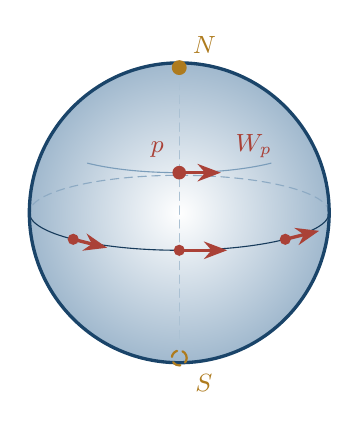
\begin{tikzpicture}[>=Stealth,scale=1.12,line cap=round,line join=round]
% Rzut ortogonalny P(x,y,z)=(x,(y+\sqrt{15}z)/4), ze skalą 1.7.
\shade[inner color=white,outer color=manifoldblue!43] (0,0) circle (1.7);
\coordinate (N) at (0,{1.7*sqrt(15)/4});
\coordinate (S) at (0,{-1.7*sqrt(15)/4});
\draw[manifoldblue!38,densely dashed,thin] (N)--(S);
% Tylna i przednia połowa równika.
\draw[manifoldblue!52,densely dashed,thin]
  (1.7,0) arc[start angle=0,end angle=180,x radius=1.7,y radius=.425];
\draw[manifoldblue!65!black,thin]
  (-1.7,0) arc[start angle=180,end angle=360,x radius=1.7,y radius=.425];
% Widoczny łuk równoleżnika z=1/2.
\draw[manifoldblue!60,thin]
  ({1.7*sqrt(3)/2*cos(225)},
   {1.7*sqrt(15)/8+1.7*sqrt(3)/8*sin(225)})
  arc[start angle=225,end angle=315,
      x radius={1.7*sqrt(3)/2},y radius={1.7*sqrt(3)/8}];
% Wektory są rzutami W_p=(-y,x,0), ze wspólną skalą długości.
\coordinate (pL) at ({1.7*cos(225)},{.425*sin(225)});
\coordinate (pE) at (0,-.425);
\coordinate (pR) at ({1.7*cos(315)},{.425*sin(315)});
\coordinate (p) at (0,{1.7*(sqrt(15)-sqrt(3))/8});
\fill[manifoldred] (pL) circle (1.8pt);
\fill[manifoldred] (pR) circle (1.8pt);
\fill[manifoldred] (pE) circle (1.8pt);
\draw[->,very thick,manifoldred] (pL)
  -- ++({.32*1.7/sqrt(2)},{-.32*.425/sqrt(2)});
\draw[->,very thick,manifoldred] (pR)
  -- ++({.32*1.7/sqrt(2)},{.32*.425/sqrt(2)});
\draw[->,very thick,manifoldred] (pE)
  -- ++(.544,0);
\draw[->,very thick,manifoldred] (p)
  -- ++({.32*1.7*sqrt(3)/2},0)
  node[above right=2pt,font=\small] {$W_p$};
\draw[manifoldblue!75!black,very thick] (0,0) circle (1.7);
\fill[manifoldred] (p) circle (2.2pt)
  node[above left=3pt,font=\small] {$p$};
\fill[manifoldgold!85!black] (N) circle (2.4pt)
  node[above right=2pt,font=\small] {$N$};
\draw[manifoldgold!85!black,densely dashed,thick] (S) circle (2.4pt)
  node[below right=3pt,font=\small] {$S$};
\end{tikzpicture}
\caption{Pole $X$ na sferze, oglądane przez $W_p=(-y,x,0)$ w $\R^3$.
Strzałki są styczne do
równoleżników i wskazują obrót wokół osi $z$. Bieguny $N$ i $S$
są zerami pola; przerywana obwódka oznacza zasłonięty biegun $S$.}
\label{fig:pole-obrotowe-na-sferze}
\end{figure}

\begin{uwaga}[Dwa sposoby obliczania pochodnej funkcji]
Gdy znamy współczynniki pola w mapie, obliczamy $X(f)(p)$
ze wzoru $X=\sum_iX^i\partial_{x^i}$, tak jak na okręgu.
Jeśli $M$ jest gładką podrozmaitością zanurzoną w $\R^N$,
możemy zamiast tego wybrać lokalne gładkie przedłużenie
$\widetilde f$ funkcji $f$ z $M$ do otoczenia $p$ w $\R^N$.
Takie przedłużenie istnieje: w lokalnym modelu, w którym $M$
jest zadana przez zerowe współrzędne normalne, nadajemy
$\widetilde f$ tę samą wartość niezależnie od tych współrzędnych.
Wtedy
$X_p(f)=W_p\cdot\nabla\widetilde f(p)$, gdzie
$(\dd\iota)_pX_p=W_p$: liczymy pochodną $\widetilde f$
wzdłuż krzywej w $M$ o wektorze stycznym $X_p$.
Wynik nie zależy od przedłużenia:
różnica dwóch przedłużeń znika na $M$, więc jej pochodna
wzdłuż każdej krzywej na $M$ jest równa zeru.
\end{uwaga}

\begin{uwaga}[Pole wzdłuż odwzorowania]
Dla gładkiego $F\colon M\to N$ i $X\in\X(M)$ wektory
$\dd F_p(X_p)$ leżą w przestrzeniach $T_{F(p)}N$.
Tworzą \emph{pole wzdłuż $F$}, czyli gładką sekcję wiązki cofniętej
\[
 F^*TN=\{(p,v):p\in M,\ v\in T_{F(p)}N\}\longrightarrow M,
 \qquad(p,v)\longmapsto p.
\]
Jeśli $x^i$ i $y^a$ są odpowiednio współrzędnymi na $M$ i $N$,
to współrzędne tego przekroju nad $p$ mają postać
$\sum_i X^i(p)\,\partial_i(y^a\circ F)(p)$.
Są gładkie, bo $X^i$ i $y^a\circ F$ są gładkie.
Pole wzdłuż $F$ ma za punkt bazowy $p\in M$, nawet gdy dwa różne
punkty $M$ mają ten sam obraz w $N$. Aby pochodziło od pola $Y$ na $N$,
musielibyśmy mieć
\[
 Y_{F(p)}=\dd F_p(X_p)\qquad\text{dla każdego }p\in M.
\]
Wektory po prawej stronie muszą zatem być równe przy wszystkich
przeciwobrazach jednego punktu.

Weźmy $M=N=\R$ oraz $X=\partial_t$ i oznaczmy współrzędną celu przez $y$.
Dla $F(t)=t^2$ reguła łańcucha daje
$\dd F_t(X_t)=2t\,\partial_y|_{t^2}$.
Jeśli $t>0$, punkty $t$ i $-t$ mają ten sam obraz $y=t^2$, więc
postulowane pole $Y$ musiałoby jednocześnie spełniać
\[
 Y_y=2t\,\partial_y|_y
 \qquad\text{oraz}\qquad
 Y_y=-2t\,\partial_y|_y.
\]
To niemożliwe, bo $t\ne0$. Nie otrzymujemy nawet jednoznacznego
przypisania wektora punktom obrazu $F$.

Dla $F(t)=t^3$ każdy $y\in\R$ ma dokładnie jeden przeciwobraz
$t=\sqrt[3]{y}$, więc nie ma już sprzeczności między przeciwobrazami.
Jedynym możliwym polem $Y$ byłoby jednak
\[
 \dd F_t(X_t)=3t^2\,\partial_y|_{t^3},
 \qquad
 Y_y=3|y|^{2/3}\,\partial_y|_y.
\]
Funkcja $a(y)=3|y|^{2/3}$ jest ciągła, lecz w zerze jej iloraz
różnicowy ma postać
\[
 \frac{a(h)-a(0)}{h}
 =3\,\operatorname{sgn}(h)|h|^{-1/3}\qquad(h\ne0),
\]
która nie ma skończonej granicy przy $h\to0$.
Nie istnieje więc gładkie pole $Y$ spełniające podany warunek.
Obie przeszkody dotyczą pary $(F,X)$: dla $F(t)=t^2$ i innego pola
$X=t\partial_t$ otrzymalibyśmy na przykład gładkie
$Y=2y\partial_y$ na $\R$.
Gdy $F$ jest dyfeomorfizmem, otrzymujemy natomiast pole
\[
 (F_*X)_q=\dd F_{F^{-1}(q)}X_{F^{-1}(q)}.
\]
Jest ono gładkie jako złożenie gładkich odwzorowań.
W szczególności $\varphi_*(X|_U)=\widehat X_\varphi$
ze wzoru~\eqref{eq:pole-przeniesione-mapa}.
Natomiast przyporządkowanie
$p\longmapsto(\dd\iota)_pX_p=W_p$ z obu przykładów
jest polem \emph{wzdłuż} inkluzji $\iota$;
wektory $W_p$ leżą w przestrzeniach stycznych do $\R^N$.
\end{uwaga}

\section{Nawias Liego: mierzenie nieprzemienności}
\label{sec:nawias}

Dwa pola są operatorami na funkcjach. Można je więc składać i wziąć
ich komutator.
\begin{definicja}
\emph{Nawiasem Liego} pól $X,Y\in\X(M)$ nazywamy pole $[X,Y]$ zadane przez
\begin{equation}\label{eq:nawias-def}
 [X,Y](f)=X(Y(f))-Y(X(f)),\qquad f\in C^\infty(M).
\end{equation}
\end{definicja}

Choć $X\circ Y$ jako operator jest na ogół drugiego rzędu, wyrazy z
pochodnymi drugimi znoszą się w różnicy.
\noindent\emph{Powiązanie tematyczne w Bibliotece matematycznej:} \atlasref{AA-57::aa:def:lie-algebra}{AA-57: abstrakcyjna definicja algebry Liego}.

\begin{fakt}\label{fakt:nawias-wlasnosci}
$[X,Y]$ jest polem wektorowym. Ponadto nawias jest dwuliniowy nad $\R$,
antysymetryczny i spełnia tożsamość Jacobiego
\[
 [X,[Y,Z]]+[Y,[Z,X]]+[Z,[X,Y]]=0.
\]
Jego reguła Leibniza względem funkcji ma postać
\begin{equation}\label{eq:nawias-leibniz}
 [X,fY]=f[X,Y]+X(f)Y,\qquad [fX,Y]=f[X,Y]-Y(f)X.
\end{equation}
\end{fakt}
\begin{proof}
Pokażmy najpierw, że komutator jest derywacją, choć samo
złożenie dwóch derywacji nią zazwyczaj nie jest.
Dla funkcji $f,g$ dwukrotnie stosujemy regułę Leibniza:
\begin{align*}
[X,Y](fg)
&=X\bigl(Y(f)g+fY(g)\bigr)
  -Y\bigl(X(f)g+fX(g)\bigr)\\
&=X(Yf)g+Y(f)X(g)+X(f)Y(g)+fX(Yg)\\
&\quad-Y(Xf)g-X(f)Y(g)-Y(f)X(g)-fY(Xg)\\
&=[X,Y](f)g+f[X,Y](g).
\end{align*}
Wyrazy mieszane znoszą się dokładnie parami. Komutator
jest liniowy nad $\R$ i spełnia regułę Leibniza,
więc z Twierdzenia~\ref{thm:derywacje-pola} odpowiada
gładkiemu polu wektorowemu. Z definicji natychmiast
$[X,Y]=-[Y,X]$; liniowość w obu argumentach wynika
z liniowości składania operatorów.

Sprawdźmy tożsamość Jacobiego, pokazując wszystkie
wyrazy. Wyłącznie w poniższym rachunku skracamy składanie
operatorów: $XYZ:=X\circ Y\circ Z$, czyli
$XYZ(f)=X(Y(Z(f)))$. Jako operatory na funkcjach mamy
\begin{align*}
[X,[Y,Z]]&=XYZ-XZY-YZX+ZYX,\\
[Y,[Z,X]]&=YZX-YXZ-ZXY+XZY,\\
[Z,[X,Y]]&=ZXY-ZYX-XYZ+YXZ.
\end{align*}
Suma prawych stron jest zerowa: np.\ $XYZ$ znosi się
z $-XYZ$, a analogicznie pozostałe pięć możliwych
kolejności. Ponieważ równość operatorów zachodzi na
każdej funkcji, zachodzi równość pól wektorowych.

Na koniec stosujemy definicję do dowolnej funkcji $g$:
\begin{align*}
[X,fY](g)
 &=X\bigl(fY(g)\bigr)-fY\bigl(X(g)\bigr)
  =X(f)Y(g)+f[X,Y](g),\\
[fX,Y](g)
 &=fX\bigl(Y(g)\bigr)-Y\bigl(fX(g)\bigr)
  =f[X,Y](g)-Y(f)X(g).
\end{align*}
Funkcje rozróżniają pola, zatem są to dokładnie
równości~\eqref{eq:nawias-leibniz}.
\end{proof}

W mapie, jeśli $X=X^i\partial_i$ i $Y=Y^j\partial_j$, to
\begin{equation}\label{eq:nawias-wspolrzedne}
 [X,Y]=\sum_{j=1}^{n}\left(\sum_{i=1}^{n}
 X^i\frac{\partial Y^j}{\partial x^i}-
 Y^i\frac{\partial X^j}{\partial x^i}\right)\partial_j.
\end{equation}
Istotnie, współczynnik przy $\partial_j$ jest równy
$[X,Y](x^j)=X(Y^j)-Y(X^j)$; na funkcjach lokalnych możemy
działać dzięki lokalności derywacji. Tu i dalej $\partial_i$
skraca $\partial/\partial x^i$, a powtórzony indeks w zapisie
takim jak $X^i\partial_i$ oznacza sumowanie po tym indeksie.
Ważny wniosek: $[\partial_i,\partial_j]=0$ w układzie współrzędnych,
ale pola tworzące ogólną ramkę lokalną
(Definicja~\ref{def:ramka-lokalna}) nie muszą komutować.
Na przykład ramka $e_1=\partial_x$,
$e_2=x\partial_x+\partial_y$ z
Przykładu~\ref{prz:ramka-plaszczyzna} spełnia
\[
 [e_1,e_2]
 =[\partial_x,x\partial_x]+[\partial_x,\partial_y]
 =\partial_x(x)\partial_x+x[\partial_x,\partial_x]+0
 =\partial_x=e_1,
\]
gdzie użyliśmy reguły~\eqref{eq:nawias-leibniz}.
Nie może więc być ramką współrzędnościową żadnej mapy.
Ramkę, w której nie wszystkie nawiasy pól bazowych znikają,
nazywamy \emph{nieholonomiczną}; określenie „ruchoma”
podkreśla natomiast gładką zależność bazy od punktu.

Co sprawdza nawias? Wykonajmy krótki ruch najpierw wzdłuż $X$,
potem wzdłuż $Y$, i porównajmy go z ruchami w odwrotnej kolejności.
Końcowe punkty mogą się różnić. Jeśli oba ruchy trwają czas $t$,
to w mapie $x$ wokół $p$ różnica współrzędnych punktów końcowych
(kolejność $X,Y$ minus $Y,X$) ma postać
$t^2\,\dd x_p([X,Y]_p)+O(t^3)$. Dokładny rachunek z przepływami podamy
niżej przy Rysunku~\ref{fig:komutator-przeplywow}.
Jeśli $[X,Y]$ znika na otoczeniu, lokalne przepływy tych pól
komutują (Stwierdzenie~\ref{prop:inwarianty}).
Nawias wykrywa także, czy ruchy wzdłuż pól stycznych do rozkładu
wytwarzają kierunek poza nim; do tego wrócimy po przykładach.

\begin{przyklad}[Ścinanie płaszczyzny]\label{prz:scinanie}
Niech $X=\partial_x$ i $Y=x\partial_y$ na $\R^2$.
Ze wzoru \eqref{eq:nawias-wspolrzedne} współczynnik przy
$\partial_x$ wynosi $X(0)-Y(1)=0$, a przy $\partial_y$
$X(x)-Y(0)=1$. Zatem $[X,Y]=\partial_y$.
Najpierw przesunięcie w kierunku $x$
zmienia prędkość pionową $Y$; wykonanie ruchów w odwrotnej kolejności
daje inny wynik. Pole $Y$ ma zera na osi $x=0$ i nie jest polem
przesunięcia o stałej prędkości.
\end{przyklad}

\begin{przyklad}[Obrót i skalowanie]
Dla $R=-y\partial_x+x\partial_y$ i $E=x\partial_x+y\partial_y$
na $\R^2$ współczynniki nawiasu wynoszą
$[R,E]^x=R(x)-E(-y)=-y-(-y)=0$ i
$[R,E]^y=R(y)-E(x)=x-x=0$.
Mamy więc $[R,E]=0$. Obrót i jednolite powiększenie
można wykonywać w dowolnej kolejności. Jeśli zaś
$X=\partial_x$, $Y=x\partial_y$, to wynik jest niezerowy
mimo że w punkcie $(0,0)$ mamy $Y=0$; nawias uwzględnia zmienność
pola w otoczeniu punktu.
\end{przyklad}



\begin{uwaga}[Rozkłady styczne i twierdzenie Frobeniusa]
Rozkład styczny wybiera w każdym punkcie $p$ podprzestrzeń
$\mathcal D_p\subset T_pM$ dopuszczalnych kierunków ruchu.
\emph{Gładkim rozkładem stałego rzędu} $0\leq k\leq n=\dim M$
nazywamy podwiązkę $\mathcal D\subset TM$ lokalnie rozpiętą
przez $k$ gładkich, punktowo liniowo niezależnych pól.
Pytamy, czy przez każdy punkt przechodzi lokalna
$k$-wymiarowa podrozmaitość $L$, dla której
$T_qL=\mathcal D_q$ w każdym $q\in L$.
Nazywamy ją \emph{podrozmaitością całkową} rozkładu.

Rozkład jest \emph{inwolutywny}, jeśli $[X,Y]$ jest jego sekcją
dla dowolnych lokalnych sekcji $X,Y$ rozkładu.
Wystarczy to sprawdzić na polach lokalnej bazy:
jeśli ich nawiasy należą do $\mathcal D$, to reguła
Leibniza~\eqref{eq:nawias-leibniz} daje tę samą własność
dla ich kombinacji o gładkich współczynnikach.
Twierdzenie Frobeniusa mówi, że jest to dokładnie warunek
istnienia przy każdym punkcie współrzędnych $(u^1,\ldots,u^n)$,
w których
\[
 \mathcal D=\operatorname{span}
 (\partial_{u^1},\ldots,\partial_{u^k}).
\]
Plasterki o stałych $u^{k+1},\ldots,u^n$ są wtedy lokalnymi
podrozmaitościami całkowymi, czyli fragmentami liści.

Na przykład na $\R^3$ pola
\[
 X=\partial_x+y\partial_z,\qquad
 Y=\partial_y+x\partial_z
\]
rozpinają rozkład $\mathcal D=\ker\dd(z-xy)$.
Rzeczywiście, $X(z-xy)=Y(z-xy)=0$, a pola są wszędzie
liniowo niezależne. Ich nawias znika:
$[X,Y]=\partial_z-\partial_z=0$.
Podrozmaitościami całkowymi są powierzchnie $z-xy=c$,
gdyż ich przestrzenie styczne są jądrami różniczki $\dd(z-xy)$.
Nie trzeba jednak wymagać, by wszystkie pola w rozkładzie
komutowały: $[X,xY]=Y\ne0$, lecz $Y$ nadal należy do
$\mathcal D$.

Inaczej jest dla rozkładu na $\R^3$
\[
 \mathcal D
 =\operatorname{span}\{\partial_x,\partial_y+x\partial_z\}.
\]
Nawias generatorów jest równy $\partial_z$, który nie należy do $\mathcal D$.
Składowe $x,y$ wymuszają bowiem zerowe współczynniki
ewentualnej kombinacji generatorów dającej $\partial_z$.
Nie ma zatem powierzchni, których przestrzenie styczne pokrywałyby się
z tym rozkładem. Dwa dozwolone ruchy wytwarzają tu
kierunek $\partial_z$ poza rozkładem.
Konieczność warunku jest widoczna już w mapie
plasterkowej: składowe normalne pól stycznych znikają na
podrozmaitości, więc ich pochodne w kierunkach stycznych również
tam znikają; wzór~\eqref{eq:nawias-wspolrzedne} pokazuje,
że nawias jest styczny. Dowód dostateczności podamy po twierdzeniu
o prostowaniu pola, w Stwierdzeniu~\ref{prop:frobenius-lokalny}.
Zastosujemy je później do lokalnego rozkładu metryki
w Twierdzeniu~\ref{thm:holonomia-lokalny-produkt}.
\end{uwaga}

\section{Krzywe całkowe i równania różniczkowe na rozmaitości}
\label{sec:krzywe}

Pole przypisuje prędkość każdemu punktowi, a krzywa całkowa opisuje
ruch zgodny z tymi prędkościami. Wektor styczny do krzywej w chwili $t$
należy do $T_{\gamma(t)}M$, dlatego porównujemy go z wartością pola
\emph{w aktualnym punkcie} $\gamma(t)$, nie z wartością w punkcie
początkowym. Obraz krzywej jest jej śladem geometrycznym; przedział
czasu i parametryzacja zapisują dodatkowo, jak szybko ten ślad przebiegamy.

\begin{definicja}
\emph{Krzywą całkową} pola $X$ nazywamy krzywą klasy $C^1$
\index{krzywa calkowa@Krzywa całkowa}
$\gamma\colon I\to M$ na otwartym przedziale $I\subset\R$ spełniającą
\begin{equation}\label{eq:krzywa-calkowa}
 \gamma'(t)=X_{\gamma(t)}.
\end{equation}
Jeśli $0\in I$ i $\gamma(0)=p$, mówimy o krzywej wychodzącej z $p$.
Jest \emph{maksymalna}, gdy nie daje się przedłużyć jako rozwiązanie
na większy przedział.
\end{definicja}

W mapie $(U,\varphi)$, gdzie $\varphi=(x^1,\ldots,x^n)$,
niech $x(t)=\varphi(\gamma(t))$ dla krzywej $\gamma$ pozostającej w $U$.
Jeśli $X|_U=\sum_i X_\varphi^i\partial_{x^i}$,
to warunek~\eqref{eq:krzywa-calkowa} staje się układem równań
różniczkowych zwyczajnych (ODE)
\[
 \frac{\dd x^i}{\dd t}
 =X_\varphi^i(\gamma(t))
 =\bigl(X_\varphi^i\circ\varphi^{-1}\bigr)(x(t)),
 \qquad i=1,\ldots,n.
\]
Krzywa nie musi być prostą nawet wtedy, gdy wektory pola rysujemy
jako małe strzałki. W każdym swoim punkcie porusza się w kierunku
aktualnej strzałki; prędkość także jest przez nią określona.

\begin{twierdzenie}[Istnienie, jednoznaczność i zależność od danych]
\label{thm:ode}
Dla każdego $p\in M$ istnieje dokładnie jedna maksymalna krzywa
całkowa $\gamma_p\colon I_p\to M$ pola $X$, gdzie $I_p$ jest otwartym
przedziałem zawierającym $0$ i $\gamma_p(0)=p$.
Rozwiązania zależą gładko od czasu i punktu początkowego tam,
gdzie są określone.
\end{twierdzenie}
\begin{proof}
\emph{Krok 1: konstrukcja w mapie.}
Wybierzmy mapę $\varphi=(u^1,\ldots,u^n)\colon U\to D=\varphi(U)\subset\R^n$
wokół punktu $p$ i połóżmy $u_0:=\varphi(p)$. Dla $v\in D$ definiujemy
\[
F(v):=(\dd\varphi)_{\varphi^{-1}(v)}
X_{\varphi^{-1}(v)}\in T_vD\cong\R^n.
\]
Współrzędnie
$F(v)=\bigl(X_\varphi^1(\varphi^{-1}(v)),\ldots,
X_\varphi^n(\varphi^{-1}(v))\bigr)$.

Pokażemy, że krzywe całkowe pola $X$ pozostające w $U$ odpowiadają
dokładnie rozwiązaniom równania $u'=F(u)$.

Niech najpierw $\gamma\colon I\to U$ będzie krzywą całkową pola $X$,
czyli $\gamma'(t)=X_{\gamma(t)}$, i połóżmy
$u(t):=\varphi(\gamma(t))$. Z reguły łańcuchowej
\[
u'(t)
=(\dd\varphi)_{\gamma(t)}\gamma'(t)
=(\dd\varphi)_{\gamma(t)}X_{\gamma(t)}
=F(u(t)),
\]
ponieważ $\varphi^{-1}(u(t))=\gamma(t)$. Jeśli dodatkowo
$\gamma(0)=p$, to $u(0)=\varphi(p)=u_0$.

Odwrotnie, niech $u\colon I\to D$ spełnia $u'(t)=F(u(t))$ oraz
$u(0)=u_0$, i zdefiniujmy $\gamma(t):=\varphi^{-1}(u(t))$.
Ponownie z reguły łańcuchowej oraz definicji $F$ mamy
\begin{align*}
\gamma'(t)
=(\dd\varphi^{-1})_{u(t)}u'(t)
=(\dd\varphi^{-1})_{u(t)}F(u(t))
=(\dd\varphi^{-1})_{u(t)}
  (\dd\varphi)_{\gamma(t)}X_{\gamma(t)}
=X_{\gamma(t)},
\end{align*}
gdyż $u(t)=\varphi(\gamma(t))$ oraz
$(\dd\varphi^{-1})_{\varphi(\gamma(t))}
\circ(\dd\varphi)_{\gamma(t)}
=\operatorname{id}_{T_{\gamma(t)}M}$.
Ponadto $\gamma(0)=\varphi^{-1}(u_0)=p$.

Otrzymujemy więc równoważność problemów
\[
\gamma'(t)=X_{\gamma(t)},\quad \gamma(0)=p
\qquad\Longleftrightarrow\qquad
u'(t)=F(u(t)),\quad u(0)=\varphi(p).
\]
Problem krzywych całkowych pola $X$ sprowadza się zatem lokalnie
do klasycznego zagadnienia początkowego dla układu ODE w $\R^n$.
Wystarczy więc skonstruować rozwiązanie $u'=F(u)$ w $D$,
a następnie wrócić przez $\varphi^{-1}$.
Wybierzmy $r>0$ tak, aby domknięta kula
$\overline B_{2r}(u_0)$ leżała w $D$.
Na tej kuli istnieją stałe $A,L\geq 0$ spełniające
$\|F(u)\|\leq A$ oraz $\|\D F(u)\|\leq L$.
Twierdzenie o wartości średniej daje
$\|F(u)-F(v)\|\leq L\|u-v\|$ dla punktów tej kuli.
Wybierzmy $h>0$ tak, aby $hA<r$ i $hL<1$
(gdy $A=0$ lub $L=0$, odpowiedni warunek jest automatyczny).

Dla każdego warunku początkowego $a\in B_r(u_0)$ rozważmy
zupełną przestrzeń metryczną krzywych ciągłych
$z\colon[-h,h]\to\overline B_{2r}(u_0)$ z metryką supremum.
Jest zupełna jako domknięty podzbiór przestrzeni Banacha
$C([-h,h],\R^n)$.
Operator Picarda
\[
 (\mathcal T_a z)(t)=a+\int_0^t F(z(\tau))\,\dd\tau,
 \qquad t\in[-h,h],
\]
jest dobrze określony także dla $t<0$: wtedy całkujemy po
$[t,0]\subset[-h,h]$ z przeciwnym znakiem. Ponieważ $|t|\leq h$,
odwzorowuje tę przestrzeń w siebie:
\[
 \|\mathcal T_a z(t)-u_0\|
 \leq\|a-u_0\|+|t|A<r+hA<2r.
\]
Podobnie z oszacowania Lipschitza dla $F$ otrzymujemy
$\|\mathcal T_a z-\mathcal T_a w\|_\infty
 \leq hL\|z-w\|_\infty$.
Z twierdzenia Banacha o punkcie stałym --- kontrakcja niepustej
zupełnej przestrzeni metrycznej ma dokładnie jeden punkt stały ---
otrzymujemy dokładnie jeden punkt stały $z_a$, czyli krzywą spełniającą
\[
 z_a(t)=a+\int_0^t F(z_a(\tau))\,\dd\tau.
\]
Jest to równanie całkowe odpowiadające zagadnieniu początkowemu
$z_a'(t)=F(z_a(t))$, $z_a(0)=a$. Istotnie, po zróżniczkowaniu
równania całkowego otrzymujemy $z_a'(t)=F(z_a(t))$ dla
$t\in(-h,h)$, a podstawienie $t=0$ daje $z_a(0)=a$.
Jest ona tam gładka w czasie: z ciągłości $z_a$ i gładkości $F$
równanie $z_a'=F(z_a)$ daje kolejno wszystkie pochodne po czasie.
Lokalna jednoznaczność dotyczy także dowolnego innego rozwiązania
$w$ przez $a$. Ciągłość $w$ pozwala wybrać $0<\delta\leq h$ tak,
aby $[-\delta,\delta]$ leżał w dziedzinie $w$ i
$w([-\delta,\delta])\subset\overline B_{2r}(u_0)$.
Ograniczamy $z_a$ do tego samego przedziału i rozpatrujemy na
$C([-\delta,\delta],\overline B_{2r}(u_0))$ operator
\[
 (\mathcal T_a^{(\delta)}z)(t)
 =a+\int_0^t F(z(\tau))\,\dd\tau,\qquad |t|\leq\delta.
\]
Jest on kontrakcją ze stałą $\delta L\leq hL<1$; zarówno $w$,
jak i $z_a$ po ograniczeniu są jego punktami stałymi, więc są równe.

\emph{Krok 2: zależność od punktu początkowego.}
Z równań całkowych dla $z_a$ i $z_b$ oraz z oszacowania
kontrakcji otrzymujemy
\[
 \|z_a-z_b\|_\infty
 \leq \|a-b\|+hL\|z_a-z_b\|_\infty,
 \qquad
 \|z_a-z_b\|_\infty\leq\frac{\|a-b\|}{1-hL}.
\]
To dowodzi najpierw ciągłej zależności, jednak do gładkości
potrzeba więcej. Dla ustalonego $a$ rozwiążmy liniowe
równanie całkowe dla macierzy $J_a(t)$:
\[
 J_a(t)=I+\int_0^t\D F(z_a(\tau))J_a(\tau)\,\dd\tau.
\]
Operator po prawej, działający na ciągłe funkcje o wartościach
macierzowych, również ma stałą kontrakcji $hL<1$.
Istnieje więc jedyne $J_a$; spełnia ono równanie
wariacyjne $J_a'=\D F(z_a)J_a$, $J_a(0)=I$.

Sprawdźmy, że jest to rzeczywiście pochodna względem $a$.
Niech $v$ będzie na tyle małe, aby $a+v\in B_r(u_0)$, i połóżmy
\[
\delta:=z_{a+v}-z_a.
\]
Z wcześniejszego oszacowania ciągłej zależności mamy
$\|\delta\|_\infty\leq \|v\|/(1-hL)$.

Ponieważ $\D^2F$ jest ograniczona na $\overline B_{2r}(u_0)$,
rozwinięcie Taylora na odcinku między $z_a(\tau)$ i
$z_{a+v}(\tau)=z_a(\tau)+\delta(\tau)$ daje, z pewną stałą
$C$ niezależną od $v$ i $\tau$,
\[
\|F(z_a(\tau)+\delta(\tau))-F(z_a(\tau))
      -\D F(z_a(\tau))\delta(\tau)\|
\leq C\|\delta(\tau)\|^2
\leq C\|\delta\|_\infty^2.
\]

Równania całkowe dla $z_{a+v}$ i $z_a$ mają postać
\[
z_{a+v}(t)=a+v+\int_0^t F(z_{a+v}(\tau))\,\dd\tau,
\qquad
z_a(t)=a+\int_0^t F(z_a(\tau))\,\dd\tau.
\]
Po ich odjęciu otrzymujemy
\[
\delta(t)
=
v+\int_0^t
\bigl(F(z_a(\tau)+\delta(\tau))-F(z_a(\tau))\bigr)\,\dd\tau.
\]
Z kolei z równania dla $J_a$ po zastosowaniu go do wektora $v$ mamy
\[
J_a(t)v
=
v+\int_0^t \D F(z_a(\tau))J_a(\tau)v\,\dd\tau.
\]

Definiujemy
\[
R(t):=\delta(t)-J_a(t)v
      =z_{a+v}(t)-z_a(t)-J_a(t)v.
\]
Odejmując dwa ostatnie równania całkowe, dostajemy
\[
R(t)
=
\int_0^t
\Bigl(
F(z_a+\delta)-F(z_a)-\D F(z_a)J_av
\Bigr)(\tau)\,\dd\tau.
\]
W wyrażeniu pod całką dodajemy i odejmujemy
$\D F(z_a(\tau))\delta(\tau)$. Ponieważ
$\delta-J_av=R$, otrzymujemy
\[
R(t)
=
\int_0^t \D F(z_a(\tau))R(\tau)\,\dd\tau
+
\int_0^t
\Bigl(
F(z_a+\delta)-F(z_a)-\D F(z_a)\delta
\Bigr)(\tau)\,\dd\tau.
\]
Stąd, korzystając z $\|\D F(z_a(\tau))\|\leq L$ oraz z oszacowania
reszty Taylora,
\[
\|R(t)\|
\leq |t|L\|R\|_\infty
     +|t|C\|\delta\|_\infty^2.
\]
Biorąc supremum po $|t|\leq h$, dostajemy
\[
\|R\|_\infty
\leq hL\|R\|_\infty+hC\|\delta\|_\infty^2
\leq hL\|R\|_\infty
+\frac{hC}{(1-hL)^2}\|v\|^2.
\]
Ponieważ $hL<1$, po przeniesieniu pierwszego składnika na lewą stronę
otrzymujemy
\[
\|R\|_\infty
\leq
\frac{hC}{(1-hL)^3}\|v\|^2
=
O(\|v\|^2).
\]
Zatem $\|R\|_\infty=O(\|v\|^2)$, co daje pochodną
$\D_a z_a=J_a$ jako odwzorowania do przestrzeni krzywych
ciągłych na $[-h,h]$. Dla jej ciągłości rozpiszmy
oszacowanie rozwiązań równania macierzowego.
Z równania dla $J_a$ najpierw
$\|J_a\|_\infty\leq1+hL\|J_a\|_\infty$,
czyli $\|J_a\|_\infty\leq(1-hL)^{-1}$.
Niech $A_a(\tau)=\D F(z_a(\tau))$.
Odejmując równania dla $J_a,J_b$ i dodając pod całką
$A_aJ_b-A_aJ_b$, otrzymujemy
\[
 J_a(t)-J_b(t)=\int_0^t
 \bigl(A_a(J_a-J_b)+(A_a-A_b)J_b\bigr)(\tau)\,\dd\tau.
\]
Stąd
$\|J_a-J_b\|_\infty
\leq hL\|J_a-J_b\|_\infty
+h\|A_a-A_b\|_\infty/(1-hL)$.
Przeniesienie pierwszego składnika na lewą stronę daje
\[
 \|J_a-J_b\|_\infty
 \leq\frac{h}{(1-hL)^2}
 \|\D F(z_a)-\D F(z_b)\|_\infty.
\]
Prawa strona dąży do zera dla $b\to a$, dzięki ciągłości
$a\mapsto z_a$ i jednostajnej ciągłości $\D F$ na zwartej kuli.
Dalsze pochodne otrzymujemy w ten sam sposób, rozdzielając
konstrukcję kandydata od sprawdzenia, że jest pochodną.
Rozpiszmy jeszcze drugi krok. Kandydat na drugą pochodną
$H_a(t)[v,w]$, dwuliniowy względem $v,w\in\R^n$, spełnia
\[
 H_a(t)[v,w]=\int_0^t\bigl(
 \D F(z_a)H_a[v,w]
 +\D^2F(z_a)[J_av,J_aw]\bigr)(\tau)\,\dd\tau.
\]
Na przestrzeni ciągłych krzywych o wartościach w odwzorowaniach
dwuliniowych część zależna od $H_a$ ma stałą kontrakcji $hL$.
Istnieje zatem dokładnie jeden taki $H_a$; jest on dwuliniowy,
bo równanie i jego wyraz wymuszający są dwuliniowe w $v,w$.

Pokażmy, że $H_a=\D_aJ_a$. Dla małego $v$ oznaczmy
$\Delta z=z_{a+v}-z_a$ i $\Delta J=J_{a+v}-J_a$ oraz
$A_a(\tau)=\D F(z_a(\tau))$. Z równań dla $J_{a+v}$ i $J_a$
po odjęciu wynika, że
\[
\Delta J(t)=\int_0^t\bigl(A_a\Delta J
 +(A_{a+v}-A_a)J_{a+v}\bigr)(\tau)\,\dd\tau.
\]
Z oszacowania~$\|\Delta z\|_\infty=O(\|v\|)$ oraz
ograniczoności $\D^2F$ na zwartej kuli dostajemy
$\|A_{a+v}-A_a\|_\infty=O(\|v\|)$.
Wcześniejsze oszacowanie dla $J_a-J_b$ daje wobec tego
$\|\Delta J\|_\infty=O(\|v\|)$.
Ponadto dowiedziona różniczkowalność $z_a$ daje
$\|\Delta z-J_av\|_\infty=O(\|v\|^2)$.
Ponieważ $\D^3F$ jest ograniczona na tej samej kuli,
wzór Taylora zastosowany do $\D F$ daje
\[
\bigl\|A_{a+v}-A_a
 -\D^2F(z_a)[J_av,\cdot]\bigr\|_\infty
 =O(\|v\|^2).
\]
Niech $R_v:=\Delta J-H_a[v,\cdot]$.
Odejmując równanie dla $H_a[v,\cdot]$ od równania dla $\Delta J$,
otrzymujemy
\begin{align*}
R_v(t)=\int_0^t\bigl(&A_aR_v
 +\bigl(A_{a+v}-A_a-\D^2F(z_a)[J_av,\cdot]\bigr)J_a\\
 &+(A_{a+v}-A_a)\Delta J\bigr)(\tau)\,\dd\tau.
\end{align*}
Ostatnie dwa składniki pod całką mają normę supremum
$O(\|v\|^2)$, więc
$\|R_v\|_\infty\leq hL\|R_v\|_\infty+O(\|v\|^2)$.
Ponieważ $hL<1$, mamy $\|R_v\|_\infty=O(\|v\|^2)$,
co dowodzi $\D_aJ_a=H_a$.
Ciągłość $a\mapsto H_a$ wynika z oszacowania kontrakcyjnego:
$z_a$ i $J_a$ zależą ciągle od $a$, więc współczynnik
$\D F(z_a)$ i wymuszenie $\D^2F(z_a)[J_a,J_a]$ są
ciągłe w normie supremum.

Ogólnie, dla $k\ge3$, połóżmy $Z_0=z_a$ i załóżmy,
że pochodne $Z_j=\D_a^j z_a$ dla $1\le j<k$
już istnieją i są ciągłe w $a$ jako krzywe na $[-h,h]$.
W $k$-krotnym różniczkowaniu złożenia $F(z_a)$ jedyny wyraz
zawierający nieznane $Z_k$ to $\D F(z_a)Z_k$.
Pozostałe wyrazy tworzą znane ciągłe wymuszenie $G_k$.
Można je zapisać bez przemilczanych współczynników.
Niech $\mathcal P_k$ oznacza zbiór podziałów zbioru
$\{1,\ldots,k\}$ na niepuste bloki. Dla bloku $B$ oznaczmy
\[
 \xi_B=Z_{|B|}(a,t)[v_i:i\in B].
\]
Jeśli $\pi=\{B_1,\ldots,B_m\}$, to $m=|\pi|$ i
\[
G_k(a,t)[v_1,\ldots,v_k]
=\sum_{\substack{\pi\in\mathcal P_k\\|\pi|\ge2}}
 \D^{|\pi|}F(z_a(t))
 [\xi_{B_1},\ldots,\xi_{B_m}].
\]
Kolejność bloków jest obojętna, bo pochodne $\D^mF$ są symetryczne.
Zapis $[v_i:i\in B]$ oznacza argumenty o indeksach z bloku $B$.
Każdy blok ma co najwyżej $k-1$ elementów, więc wszystkie
występujące tutaj $Z_j$ są już znane. Dla $k=2$ wzór daje
wyraz $\D^2F(z_a)[J_av,J_aw]$ z równania dla $H_a$.
Kandydata $Z_k$ określa więc równanie
\[
 Z_k(a,t)=\int_0^t\bigl(\D F(z_a(\tau))Z_k(a,\tau)
                         +G_k(a,\tau)\bigr)\,\dd\tau
 \qquad(k\ge3).
\]
Na ciągłych krzywych o wartościach w przestrzeni odwzorowań
$k$-liniowych jego prawa strona jest kontrakcją ze stałą $hL$.
Sprawdźmy, że jest to rzeczywiście pochodna $Z_{k-1}$.
Oznaczmy $A_a=\D F(z_a)$ i $\Delta Q=Q_{a+v}-Q_a$.
Ponieważ $G_{k-1}$ zawiera tylko $Z_j$ z $j\le k-2$,
a ich pochodne $Z_{j+1}$ są znane, odwzorowanie
$a\mapsto G_{k-1}(a,\cdot)$ jest klasy $C^1$ w normie supremum.
Także $a\mapsto A_a$ jest klasy $C^1$, z pochodną
$\D_aA_a[v]=\D^2F(z_a)[J_av,\cdot]$.
Różniczkując formalnie równanie dla $Z_{k-1}$, dostajemy
równanie dla kandydata $K[v,\cdot]$:
\[
K(t)=\int_0^t\bigl(A_aK
 +\D_aA_a[v]Z_{k-1}(a)
 +\D_aG_{k-1}(a)[v]\bigr)(\tau)\,\dd\tau.
\]
Reguła łańcucha zastosowana do powyższej sumy po podziałach
pokazuje, że dwa ostatnie składniki tworzą dokładnie
$G_k(a)[v,\cdot]$: różniczkowanie albo dodaje $v$ do
istniejącego bloku, albo tworzy dla niego nowy blok.
Z jednoznaczności rozwiązania równania liniowego mamy więc
$K=Z_k(a)[v,\cdot]$.

Niech $R_v:=\Delta Z_{k-1}-K$.
Po odjęciu równań dla $Z_{k-1}(a+v)$, $Z_{k-1}(a)$ i $K$
otrzymujemy
\begin{align*}
R_v(t)=\int_0^t\bigl(&A_aR_v
 +(\Delta A-\D_aA_a[v])Z_{k-1}(a)\\
 &+\Delta A\,\Delta Z_{k-1}
 +\Delta G_{k-1}-\D_aG_{k-1}(a)[v]\bigr)(\tau)\,\dd\tau.
\end{align*}
Pierwsza i ostatnia reszta mają normę $o(\|v\|)$,
bo $A_a$ i $G_{k-1}$ są różniczkowalne w normie supremum.
Ponadto $\|\Delta A\|_\infty=O(\|v\|)$ i
$\|\Delta Z_{k-1}\|_\infty=o(1)$ z ciągłości $Z_{k-1}$.
Stąd $\|R_v\|_\infty\leq hL\|R_v\|_\infty+o(\|v\|)$,
a $hL<1$ daje $R_v=o(\|v\|)$.
To dowodzi $Z_k=\D_aZ_{k-1}$.
Ponieważ $A_a$ i $G_k(a,\cdot)$ zależą ciągle od $a$,
oszacowanie kontrakcyjne zastosowane do dwóch równań dla $Z_k$
daje ciągłość $Z_k$. Indukcja dowodzi gładkości $a\mapsto z_a$.

Aby sprawdzić ciągłość pochodnych mieszanych po czasie i danych
początkowych, zdefiniujmy gładkie odwzorowania
$V_0(v)=v$ i $V_{m+1}(v)=\D V_m(v)F(v)$ na $D$.
Z równania $z_a'=F(z_a)$ i reguły łańcucha wynika indukcyjnie
$\partial_t^m z_a(t)=V_m(z_a(t))$. Prawa strona zależy
gładko od $a$ jako krzywa ciągła, a wszystkie jej pochodne
po $a$ są ciągłe wspólnie w $(t,a)$. Otrzymujemy gładkość
$(t,a)\mapsto z_a(t)$ na $(-h,h)\times B_r(u_0)$.

\emph{Krok 3: przedział maksymalny.}
Dwie krzywe całkowe wychodzące z $p$ są równe w pobliżu zera
na mocy powyższej jednoznaczności. Zbiór czasów, w których
się zgadzają, jest domknięty w części wspólnej ich
przedziałów przez ciągłość obu krzywych. Jest też otwarty:
w punkcie, w którym się zgadzają, stosujemy lokalną
jednoznaczność ponownie. Ponieważ część wspólna jest przedziałem,
krzywe pokrywają się wszędzie, gdzie obie są określone.
Można więc skleić wszystkie rozwiązania przez $p$ na sumie
ich przedziałów. Suma ta jest otwartym przedziałem $I_p$
zawierającym zero; sklejenie daje rozwiązanie, którego żadne
dalsze przedłużenie nie istnieje. Jednoznaczność w mapach
zapewnia, że konstrukcja nie zależy od wyboru współrzędnych.
Dotąd wykazaliśmy gładką zależność na wspólnym krótkim przedziale
wokół zera. Dla dowolnego $t_0\in I_{p_0}$ zwarty odcinek krzywej
od czasu $0$ do $t_0$ dzielimy na skończenie wiele fragmentów,
na których działają lokalne konstrukcje z kroków 1--2.
Ich gładkie złożenie daje wspólną dziedzinę i gładką zależność
w otoczeniu $(t_0,p_0)$. Szczegóły tego sklejania,
w tym otwartość dziedziny wszystkich par $(t,p)$,
podajemy w dowodzie Twierdzenia~\ref{thm:przeplyw}.
\end{proof}

Jeśli $X_p=0$, to jedyną krzywą wychodzącą z $p$ jest krzywa stała.
Jeśli dwie krzywe całkowe spotkają się, to po odpowiednim przesunięciu
parametru czasu pokrywają się tam, gdzie obie są określone.
Mogą więc tworzyć orbitę okresową, lecz nie mogą przecinać się
transwersalnie jako trajektorie tego samego pola.

\begin{przyklad}[Punkt równowagi i zbliżanie asymptotyczne]
Na $\R$ pole $X=x\partial_x$ prowadzi do równania $x'=x$.
Dla warunku początkowego $x(0)=a$ rozwiązaniem jest
$x_a(t)=ae^t$, bo $x_a'(t)=ae^t=x_a(t)$ i $x_a(0)=a$.
Jest określone dla każdego $t\in\R$, więc jest maksymalne.
Gdy $a=0$, otrzymujemy krzywą stałą: zero jest punktem
równowagi. Gdy $a>0$, krzywa pozostaje dodatnia, a gdy $a<0$
--- ujemna. W obu przypadkach $x_a(t)\to0$ przy $t\to-\infty$,
ale w żadnym skończonym czasie nie osiąga zera.
To konkretny obraz jednoznaczności: gdyby inna trajektoria
dotarła do punktu równowagi w skończonym czasie, od tej chwili
musiałaby pokrywać się z rozwiązaniem stałym.
\end{przyklad}

\begin{przyklad}[Przejście przez granicę mapy kątowej]
Wróćmy do pola $X$ na $S_r^1$ z Przykładu w
Sekcji~\ref{sec:derywacje}, otrzymanego z pola
$W=-v\partial_u+u\partial_v$ na $\R^2$.
Niech $p=(r\cos\theta_0,r\sin\theta_0)$, gdzie $\theta_0\in\R$.
Dla wszystkich $t\in\R$ określmy
\[
\gamma_p(t)=\bigl(r\cos(\theta_0+t),
                    r\sin(\theta_0+t)\bigr).
\]
Jeśli $\iota\colon S_r^1\hookrightarrow\R^2$ jest inkluzją,
to po zróżniczkowaniu dostajemy
\[
(\dd\iota)_{\gamma_p(t)}\gamma_p'(t)
=\bigl(-r\sin(\theta_0+t),r\cos(\theta_0+t)\bigr)
=W_{\iota(\gamma_p(t))}
=(\dd\iota)_{\gamma_p(t)}X_{\gamma_p(t)}.
\]
Różniczka inkluzji jest injektywna, zatem
$\gamma_p'(t)=X_{\gamma_p(t)}$.
Krzywa jest określona na całej $\R$, więc jej maksymalny
przedział to $I_p=\R$.

W mapie kątowej $U=S_r^1\setminus\{q\}$, gdzie $q=(-r,0)$,
wybieramy kąt z przedziału $(-\pi,\pi)$. Dla punktu
$p$ o kącie $\theta_0=2\pi/3$ współrzędna krzywej wynosi
$\theta(t)=2\pi/3+t$ tylko dopóki pozostaje w tym przedziale;
przy $t=\pi/3$ krzywa osiąga $q$. W tej chwili kończy się zapis
w wybranej mapie, choć sama krzywa i pole istnieją dalej.
Wystarczy przejść do mapy obejmującej $q$.
Rysunek~\ref{fig:krzywa-przez-granice-mapy} odróżnia koniec mapy
od końca przedziału istnienia rozwiązania.
\end{przyklad}

\begin{figure}[!htbp]
\centering
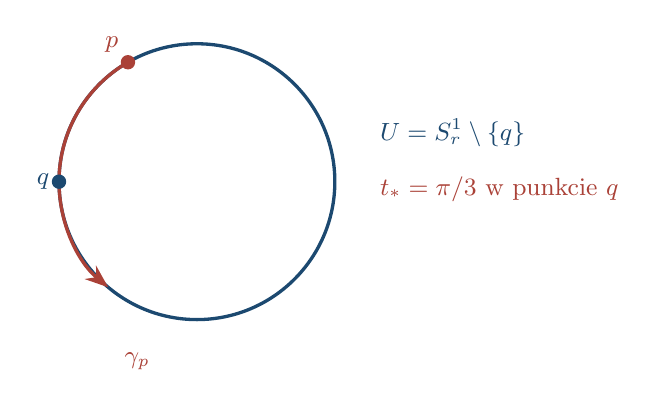
\begin{tikzpicture}[>=Stealth,scale=1.13,line cap=round,line join=round]
  \draw[manifoldblue!80!black,very thick] (0,0) circle (1.55);
  \draw[->,manifoldred,very thick]
    (120:1.55) arc[start angle=120,end angle=230,radius=1.55];
  \fill[manifoldred] (120:1.55) circle (2.3pt)
    node[above left,font=\small] {$p$};
  \fill[manifoldblue!80!black] (180:1.55) circle (2.3pt)
    node[left,font=\small] {$q$};
  \node[anchor=west,font=\small,manifoldblue!80!black]
    at (1.95,.55) {$U=S_r^1\setminus\{q\}$};
  \node[anchor=west,font=\small,manifoldred]
    at (1.95,-.08) {$t_*=\pi/3$ w punkcie $q$};
  \node[font=\small,manifoldred] at (-.67,-2.02) {$\gamma_p$};
\end{tikzpicture}
\caption{Krzywa całkowa pola obrotowego przechodzi przez $q$ w czasie
$t_*=\pi/3$. Punkt $q$ należy do okręgu, lecz nie do wybranej mapy
kątowej $U$. Czerwony łuk biegnie dalej po przekroczeniu $q$.}
\label{fig:krzywa-przez-granice-mapy}
\end{figure}

\begin{przyklad}[Obrót]
Na $\R^2$ niech $X=-y\partial_x+x\partial_y$. Układ
$x'=-y$, $y'=x$ rozwiązujemy, łącząc współrzędne w
$z=x+\mathrm{i}y$. Wtedy
$z'=-y+\mathrm{i}x=\mathrm{i}z$, więc
$(e^{-\mathrm{i}t}z)'=0$.
Dla $z(0)=a+\mathrm{i}b$ mamy
$z(t)=e^{\mathrm{i}t}(a+\mathrm{i}b)$.
Po użyciu $e^{\mathrm{i}t}=\cos t+\mathrm{i}\sin t$
i rozdzieleniu części rzeczywistej i urojonej dostajemy
\begin{equation}\label{eq:obrot}
 \gamma_{(a,b)}(t)=(a\cos t-b\sin t,\ a\sin t+b\cos t).
\end{equation}
Dla $(a,b)\ne(0,0)$ trajektorią jest okrąg o promieniu
$\sqrt{a^2+b^2}$, przebiegany przeciwnie do ruchu wskazówek zegara.
Początek układu jest punktem stałym.
\end{przyklad}

\begin{figure}[!htbp]
\centering
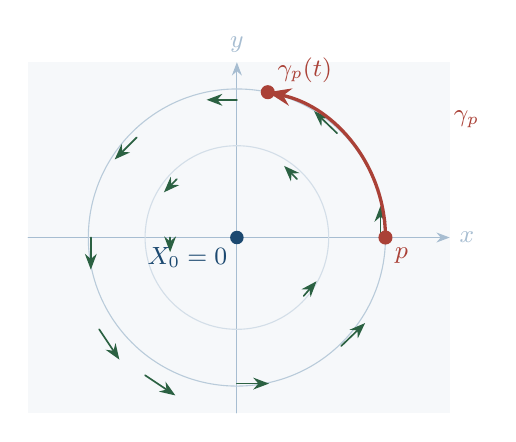
\begin{tikzpicture}[>=Stealth,scale=1.06,line cap=round]
\fill[manifoldblue!4] (-2.5,-2.1) rectangle (2.55,2.1);
\draw[->,manifoldblue!40] (-2.5,0)--(2.55,0) node[right,font=\small] {$x$};
\draw[->,manifoldblue!40] (0,-2.1)--(0,2.1) node[above,font=\small] {$y$};
\draw[manifoldblue!20] (0,0) circle (1.1);
\draw[manifoldblue!32] (0,0) circle (1.78);
\foreach \xx/\yy in {-1.65/-1.1,-1.1/-1.65,0/-1.75,1.25/-1.3,1.72/0,
 1.2/1.25,0/1.65,-1.2/1.2,-1.75/0,-.8/0,.72/.7,-.72/.7,.8/-.7}{
 \draw[->,manifoldgreen!78!black,semithick]
 (\xx,\yy)--++({-.22*\yy},{.22*\xx});}
\draw[manifoldred,very thick,->] (1.78,0)
 arc[start angle=0,end angle=78,radius=1.78];
\fill[manifoldred] (1.78,0) circle (2.4pt)
 node[below right,font=\small] {$p$};
\fill[manifoldred] ({1.78*cos(78)},{1.78*sin(78)}) circle (2.4pt)
  node[above right,font=\small] {$\gamma_p(t)$};
\fill[manifoldblue!80!black] (0,0) circle (2.3pt)
 node[below left,font=\small] {$X_0=0$};
\node[font=\small,manifoldred] at (2.75,1.42) {$\gamma_p$};
\end{tikzpicture}
\caption{Pole obrotowe $X=(-y,x)$: zielone strzałki przedstawiają wartości
pola pomniejszone wspólnym czynnikiem $0.22$,
a czerwona krzywa jest jego krzywą całkową. Strzałka pola
w każdym punkcie jest styczna do trajektorii.}
\label{fig:obrot-krzywa}
\end{figure}

\begin{przyklad}[Zmiana prędkości bez zmiany orbit]
Niech $Y=fX$, gdzie $f\colon M\to(0,\infty)$ jest funkcją gładką.
Pola $X$ i $Y$ wyznaczają te same \emph{zorientowane ślady} krzywych
całkowych: zmienia się jedynie prędkość, z jaką dana krzywa jest przebiegana.

Niech $\gamma\colon I\to M$ będzie krzywą całkową pola $X$, czyli
$\gamma'(\tau)=X_{\gamma(\tau)}$. Chcemy tę samą krzywą geometryczną
sparametryzować nowym parametrem $s$ tak, aby stała się krzywą
całkową pola $Y$.

Wybieramy $\tau_0\in I$ i definiujemy
$s(\tau):=\int_{\tau_0}^\tau\frac{\dd u}{f(\gamma(u))}$.
Ponieważ $f>0$, mamy $s'(\tau)=1/f(\gamma(\tau))>0$, zatem $s$ jest
ściśle rosnąca i wyznacza dyfeomorfizm przedziału $I$ na pewien
przedział $J$. Niech $\tau=\tau(s)$ oznacza funkcję odwrotną.
Z reguły różniczkowania funkcji odwrotnej
$\tau'(s)=1/s'(\tau(s))=f(\gamma(\tau(s)))$.

Definiujemy teraz $\eta(s):=\gamma(\tau(s))$.
Krzywe $\gamma$ i $\eta$ mają ten sam obraz w $M$, ponieważ różnią się
jedynie parametryzacją. Z reguły łańcucha
\begin{align*}
\eta'(s)
=\gamma'(\tau(s))\,\tau'(s)
=X_{\gamma(\tau(s))}\,f(\gamma(\tau(s)))
=f(\eta(s))X_{\eta(s)}
=Y_{\eta(s)}.
\end{align*}
Zatem $\eta$ jest krzywą całkową pola $Y$.

Widzimy więc, że pomnożenie pola $X$ przez dodatnią funkcję $f$
nie zmienia geometrycznych orbit pola. Zmienia jedynie sposób ich
parametryzacji w czasie, zgodnie z zależnością
$d\tau/ds=f(\eta(s))$.
Tam, gdzie $f$ jest duże, ruch względem czasu $s$ jest szybszy,
a tam, gdzie $f$ jest małe, jest wolniejszy.

Ta sama konstrukcja zastosowana do $X=\frac{1}{f}Y$
pokazuje odwrotną zależność. Zachowuje ona także maksymalność:
załóżmy, że $\gamma$ jest maksymalna, a $J$ ma skończony prawy
koniec $d$, przez który $\eta$ daje się przedłużyć jako krzywa
całkowa $Y$. Wtedy $\eta(s)\to\eta(d)$ dla $s\uparrow d$ oraz
$f(\eta(s))\to f(\eta(d))>0$. Z równania, dla ustalonego $s_0\in J$,
\[
\tau(s)=\tau(s_0)+\int_{s_0}^{s}f(\eta(u))\,\dd u
\]
wynika, że $\tau(s)$ ma skończoną granicę $\tau_*$ przy $s\uparrow d$.
Przedłużamy $\eta$ za $d$ i na tym większym przedziale
definiujemy $\widetilde\tau(s)$ przez tę samą całkę z
$f(\eta(u))$. Jej pochodna w $d$ wynosi $f(\eta(d))>0$,
więc ma lokalną odwrotność $\widetilde s$.
Ponieważ $\tau(J)=I$, liczba $\tau_*$ jest prawym końcem $I$.
Wzór $\widetilde\gamma(\tau)=\eta(\widetilde s(\tau))$
przedłuża wtedy $\gamma$ przez $\tau_*$, wbrew maksymalności.
Dla lewego końca $J$ argument jest
taki sam; przy nieskończonym końcu przedłużenie przedziału nie jest
możliwe. Wobec tego maksymalne
krzywe całkowe $X$ i $Y$ mają te same zorientowane obrazy, chociaż
ich maksymalne przedziały czasu nie muszą być takie same.

Na przykład na $\R$ rozważmy $X=\frac{\partial}{\partial x}$.
Krzywa całkowa wychodząca z $0$ ma postać $\gamma(\tau)=\tau$
i jest określona dla wszystkich $\tau\in\R$, więc pole $X$ jest zupełne.

Pomnóżmy je teraz przez $f(x)=1+x^2$. Otrzymujemy
$Y=(1+x^2)\frac{\partial}{\partial x}$.
Zmiana czasu jest dana przez
\[
s(\tau)=\int_0^\tau\frac{\dd u}{1+u^2}=\arctan\tau.
\]
Jej obrazem jest tylko przedział $(-\pi/2,\pi/2)$.
Funkcja odwrotna ma postać $\tau(s)=\tan s$, więc odpowiadająca
krzywa całkowa pola $Y$ jest dana przez
$\eta(s)=\tan s$, gdzie $s\in(-\pi/2,\pi/2)$.
Obie krzywe mają ten sam obraz, równy całej $\R$, lecz pierwsza jest
określona dla wszystkich czasów, a druga tylko dla skończonego
przedziału czasu. Zatem pomnożenie pola przez dodatnią funkcję może
zmienić jego zupełność.

Jeżeli $f$ może zmieniać znak, sytuacja jest inna: tam, gdzie $f<0$,
orientacja ruchu wzdłuż orbity zostaje odwrócona. Jeśli natomiast
$f(p)=0$, to $Y_p=f(p)X_p=0$, więc $p$ staje się punktem stałym
pola $Y$. Dlatego założenie $f>0$ jest istotne dla stwierdzenia
o zachowaniu zorientowanych orbit.
\end{przyklad}


\section{Przepływ lokalny, maksymalny i zupełny}
\label{sec:przeplyw}

Krzywe całkowe dla wszystkich punktów początkowych łączą się
w jedno odwzorowanie. W czasie $t$ przesuwamy punkt o tyle, ile
pozwala równanie~\eqref{eq:krzywa-calkowa}.

\begin{definicja}
Niech $\gamma_p\colon I_p\to M$ będzie maksymalną krzywą całkową.
\emph{Dziedziną maksymalnego przepływu} jest zbiór
$\mathcal D_X=\{(t,p)\in\R\times M:t\in I_p\}$, a
\emph{przepływem} pola $X$ odwzorowanie
\index{przeplyw pola wektorowego@Przepływ pola wektorowego}
\[
 \Phi\colon\mathcal D_X\to M,\qquad \Phi(t,p)=\Phi_t(p):=\gamma_p(t).
\]
Pole jest \emph{zupełne}, jeśli $\mathcal D_X=\R\times M$.
\end{definicja}

Przepływ łączy więc wszystkie krzywe całkowe w jedną rodzinę
odwzorowań $\Phi_t$. Dla ustalonego $t$ jego dziedziną są tylko
te punkty, których krzywe istnieją do chwili $t$; zbiór ten
może zależeć od $t$. Zupełność wymaga istnienia każdej krzywej
przez wszystkie dodatnie i ujemne czasy.
Ograniczenie $\Phi$ do prostokątnej dziedziny
$(-\varepsilon,\varepsilon)\times W\subset\mathcal D_X$,
gdzie $W\subset M$ jest otwarty, nazywamy \emph{przepływem lokalnym}.
Przepływ maksymalny wykorzystuje wszystkie dopuszczalne pary
$(t,p)\in\mathcal D_X$; przy polu zupełnym ta dziedzina staje się
całym $\R\times M$. Lokalny przepływ nie musi wysyłać $W$ w siebie:
jego wartości należą do $M$.

\begin{twierdzenie}[Podstawowe własności przepływu]
\label{thm:przeplyw}
Niech $X$ będzie gładkim polem wektorowym na $M$, a
$\gamma_p\colon I_p\to M$ maksymalną krzywą całkową spełniającą
$\gamma_p(0)=p$. Oznaczmy
$\mathcal D_X:=\{(t,p)\in\R\times M:t\in I_p\}$ oraz
$\Phi(t,p):=\gamma_p(t)$.
Wówczas $\mathcal D_X$ jest otwarty, a odwzorowanie
$\Phi\colon\mathcal D_X\to M$ jest gładkie. Ponadto:
\begin{enumerate}
\item $\Phi_0=\id_M$. Jeśli $s\in I_p$ i $q:=\Phi_s(p)$, to
$I_q=I_p-s$ oraz $\Phi_{t+s}(p)=\Phi_t(\Phi_s(p))$
dla każdego $t\in I_q$.
\item Dla $M_t:=\{p\in M:t\in I_p\}$ zbiory $M_t$ i $M_{-t}$
są otwarte, a $\Phi_t\colon M_t\to M_{-t}$ jest dyfeomorfizmem
odwrotnym do $\Phi_{-t}$.
\item Zachodzą równości
\begin{equation}\label{eq:przeplyw-generuje}
\left.\frac{\dd}{\dd t}\right|_{t=0}\Phi_t(p)=X_p,
\qquad (\dd\Phi_t)_pX_p=X_{\Phi_t(p)}
\quad (p\in M_t).
\end{equation}
\end{enumerate}
Jeśli $X$ jest zupełne, to $(\Phi_t)_{t\in\R}$ jest
jednoparametrową grupą dyfeomorfizmów $M$.
\end{twierdzenie}

\begin{proof}
\emph{Otwartość dziedziny i gładkość przepływu.}
Wyjaśnijmy najpierw cel tej części dowodu. Z poprzedniego
twierdzenia wiemy, że dla każdego $p\in M$ istnieje maksymalna
krzywa całkowa $\gamma_p$, a także że rozwiązania zależą gładko
od danych początkowych przez dostatecznie krótki czas.
Nie wiemy jednak jeszcze, czy dla ustalonego, być może dużego
$t_0\in I_{p_0}$ rozwiązania wychodzące z punktów bliskich $p_0$
istnieją aż do czasu bliskiego $t_0$. Chcemy wykazać, że istnieją
otoczenie $V$ punktu $p_0$ i liczba $\delta>0$, dla których
$ (t_0-\delta,t_0+\delta)\times V\subseteq\mathcal D_X$,
a $\Phi$ jest gładkie na tym iloczynie.

Przypomnijmy dokładnie, co daje lokalne twierdzenie o istnieniu
i gładkiej zależności. Dla każdego $q\in M$ istnieją otwarte
otoczenie $W_q$ i liczba $\varepsilon_q>0$ takie, że
\[
L_q\colon(-\varepsilon_q,\varepsilon_q)\times W_q\longrightarrow M,
\qquad L_q(u,z)=\gamma_z(u),
\]
jest dobrze określonym, gładkim odwzorowaniem. W szczególności
wszystkie rozwiązania rozpoczynające się w $W_q$ istnieją
przynajmniej przez wspólny czas $\varepsilon_q$ w obu kierunkach.
W dowodzie lokalnym można na przykład wybrać
$W_q=\varphi_q^{-1}(B(\varphi_q(q),r_q))$; jest to zbiór
punktów początkowych w $M$, nie cylinder zawierający zmienną czasu.

Ustalmy $(t_0,p_0)\in\mathcal D_X$ i najpierw załóżmy $t_0>0$.
Obraz $K:=\gamma_{p_0}([0,t_0])$ jest zwarty, gdyż jest obrazem
odcinka domkniętego przez odwzorowanie ciągłe. Wybierzmy z pokrycia
$K$ przez otoczenia $W_q$ skończone podpokrycie
$W_{q_1},\ldots,W_{q_m}$ oraz połóżmy
$\varepsilon:=\min\{\varepsilon_{q_1},\ldots,
\varepsilon_{q_m}\}>0$.
Każdy punkt $K$ należy zatem do pewnego $W_{q_i}$,
z którego można rozpocząć rozwiązanie na całym
$(-\varepsilon,\varepsilon)$. Wybierzmy podział
$0=\tau_0<\tau_1<\cdots<\tau_N=t_0$ taki, że
$\Delta_j:=\tau_{j+1}-\tau_j<\varepsilon/2$.
Rysunek~\ref{fig:przeplyw-pokrycie} przedstawia tę konstrukcję.

\begin{figure}[H]
\centering
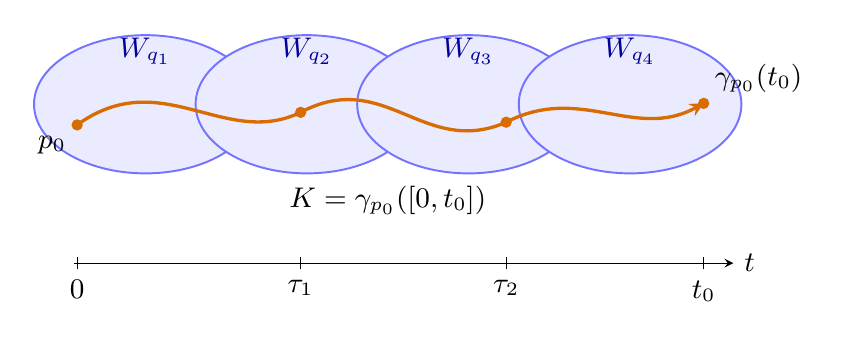
\begin{tikzpicture}[x=1cm,y=1cm,scale=1.14,transform shape,>=stealth,
    every node/.style={font=\small}]
  % Skończone pokrycie obrazu krzywej.
  \foreach \x/\i in {1.0/1,2.8/2,4.6/3,6.4/4}{
    \filldraw[fill=blue!8,draw=blue!55,line width=.7pt]
      (\x,1.75) ellipse (1.24 and .77);
    \node[blue!60!black] at (\x,2.34) {$W_{q_{\i}}$};
  }
  \draw[very thick,orange!85!black,->]
    (0.24,1.52) .. controls (1.18,2.20) and (1.88,1.25) .. (2.73,1.66)
    .. controls (3.67,2.16) and (4.10,1.15) .. (5.02,1.55)
    .. controls (5.85,1.98) and (6.45,1.34) .. (7.22,1.76);
  \fill[orange!85!black] (0.24,1.52) circle (1.8pt);
  \fill[orange!85!black] (2.73,1.66) circle (1.8pt);
  \fill[orange!85!black] (5.02,1.55) circle (1.8pt);
  \fill[orange!85!black] (7.22,1.76) circle (1.8pt);
  \node[below left] at (0.24,1.52) {$p_0$};
  \node[above right] at (7.22,1.76) {$\gamma_{p_0}(t_0)$};
  \node at (3.7,.68) {$K=\gamma_{p_0}([0,t_0])$};
  \draw[->] (.2,-.02)--(7.55,-.02) node[right] {$t$};
  \foreach \x/\lab in {.24/0,2.73/{\tau_1},5.02/{\tau_2},7.22/{t_0}}{
    \draw (\x,-.09)--(\x,.05);
    \node[below] at (\x,-.09) {$\lab$};
  }
\end{tikzpicture}

\caption{Skończone pokrycie zwartego obrazu $K$ otoczeniami,
na których obowiązuje wspólny dodatni czas lokalnego istnienia.
Podział czasu wybieramy dostatecznie drobny.}
\label{fig:przeplyw-pokrycie}
\end{figure}

Teraz dla każdego $j=0,\ldots,N-1$ oznaczmy
$z_j:=\gamma_{p_0}(\tau_j)$ i wybierzmy jeden ze zbiorów
$W_{q_i}$ zawierający $z_j$. Nazwijmy go $W_j$.
Lokalny przepływ odpowiadający temu otoczeniu oznaczmy przez
$L_j$. Ponieważ $\Delta_j<\varepsilon$, odwzorowanie
$\Psi_j\colon W_j\to M$, dane wzorem
$\Psi_j(z):=L_j(\Delta_j,z)$, jest gładkie.
Przesuwa ono punkt $z$ wzdłuż jego krzywej całkowej o czas
$\Delta_j$. Z jednoznaczności rozwiązań wynika w szczególności,
że $\Psi_j(z_j)=z_{j+1}$.

Musimy jednak uważać na dziedziny: obraz całego $W_j$ przez
$\Psi_j$ nie musi zawierać się w $W_{j+1}$. Nie możemy więc bez
dalszych przygotowań składać odwzorowań $\Psi_{j+1}$ i $\Psi_j$.
Rozwiązujemy ten problem, zmniejszając \emph{wyłącznie otoczenie
początkowego punktu $p_0$}, a nie zbiory $W_j$.

Rozpocznijmy od $U_0:=W_0$ i $F_0:=\id_{U_0}$.
Załóżmy indukcyjnie, że $U_j$ jest otwartym otoczeniem $p_0$,
a $F_j\colon U_j\to M$ jest gładkim odwzorowaniem opisującym
przesunięcie o czas $\tau_j$, przy czym $F_j(p_0)=z_j$.
Definiujemy
\[
U_{j+1}:=U_j\cap F_j^{-1}(W_j),\qquad
F_{j+1}:=\Psi_j\circ F_j\big|_{U_{j+1}}.
\]
Zbiór $U_{j+1}$ jest otwarty, ponieważ $F_j$ jest ciągłe
i $W_j$ jest otwarty. Zawiera $p_0$, gdyż
$F_j(p_0)=z_j\in W_j$. Co najważniejsze,
$F_j(U_{j+1})\subseteq W_j$, zatem następny lokalny przepływ
$\Psi_j$ rzeczywiście można zastosować do wszystkich punktów
z $U_{j+1}$. Odwzorowanie $F_{j+1}$ jest gładkie jako złożenie
odwzorowań gładkich i, na mocy jednoznaczności,
$F_{j+1}(p)=\gamma_p(\tau_{j+1})$ dla $p\in U_{j+1}$.

Dla lepszego zobrazowania pierwszych dwóch kroków oznaczmy
$p_j:=\gamma_{p_0}(\tau_j)$ i przyjmijmy
$\Psi_0(z)=\gamma_z(\tau_1-\tau_0)$,
$\Psi_1(z)=\gamma_z(\tau_2-\tau_1)$ na odpowiednich
otoczeniach $W_0$ i $W_1$. Wówczas
$U_1=U_0$ oraz $U_2=U_1\cap\Psi_0^{-1}(W_1)$. Jeśli dodatkowo wybierzemy
otoczenie $W_2$ punktu $p_2$, to
$U_3=U_2\cap(\Psi_1\circ\Psi_0)^{-1}(W_2)$
zapewnia możliwość wykonania kolejnego kroku po czasie $\tau_2$.
Rysunek~\ref{fig:przeplyw-skladanie-lokalne} pokazuje, skąd
biorą się kolejne ograniczenia otoczenia początkowego.

\begin{figure}[H]
\centering
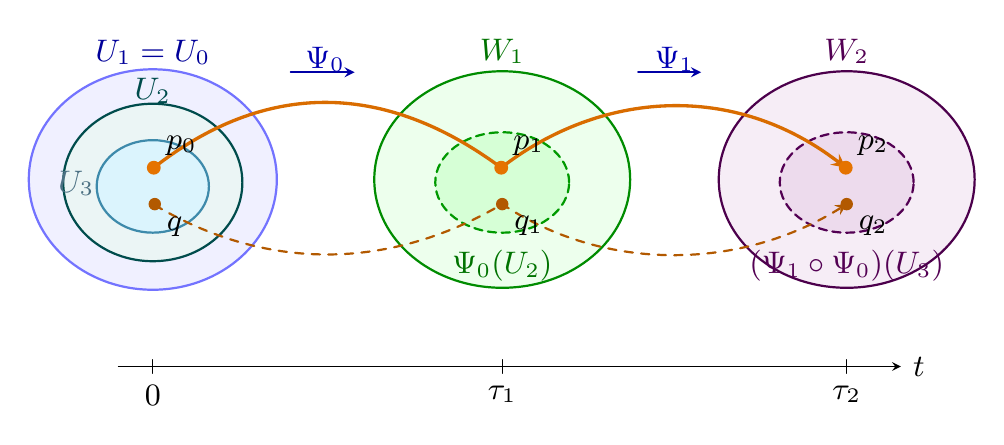
\begin{tikzpicture}[x=1cm,y=1cm,scale=1.25,transform shape,>=stealth,
    every node/.style={font=\small},line cap=round]
  % Otoczenia początkowe: U3 zawiera się w U2, a U2 w U1=U0.
  \filldraw[fill=blue!6,draw=blue!55,thick]
    (1.0,1.85) ellipse (1.26 and 1.12);
  \filldraw[fill=teal!8,draw=teal!60!black,thick]
    (1.0,1.82) ellipse (.91 and .80);
  \filldraw[fill=cyan!14,draw=cyan!65!black,thick]
    (1.0,1.78) ellipse (.57 and .47);
  \node[blue!60!black] at (1.0,3.14) {$U_1=U_0$};
  \node[teal!60!black] at (1.0,2.75) {$U_2$};
  \node[cyan!45!black,anchor=east] at (.53,1.81) {$U_3$};

  % Otoczenia w chwilach tau_1 i tau_2 oraz obrazy podzbiorów.
  \filldraw[fill=green!7,draw=green!55!black,thick]
    (4.55,1.85) ellipse (1.30 and 1.10);
  \filldraw[fill=green!16,draw=green!60!black,densely dashed,thick]
    (4.55,1.82) ellipse (.68 and .51);
  \node[green!45!black] at (4.55,3.15) {$W_1$};
  \node[green!45!black] at (4.55,.97) {$\Psi_0(U_2)$};

  \filldraw[fill=violet!7,draw=violet!60!black,thick]
    (8.05,1.85) ellipse (1.30 and 1.10);
  \filldraw[fill=violet!14,draw=violet!65!black,densely dashed,thick]
    (8.05,1.82) ellipse (.68 and .51);
  \node[violet!65!black] at (8.05,3.15) {$W_2$};
  \node[violet!65!black] at (8.05,.97) {$(\Psi_1\circ\Psi_0)(U_3)$};

  % Krzywa bazowa i krzywa punktu pobliskiego q.
  \draw[orange!85!black,very thick,->]
    (1.01,1.97) .. controls (2.15,2.86) and (3.35,2.85) .. (4.54,1.97)
    .. controls (5.55,2.75) and (6.90,2.85) .. (8.04,1.97);
  \draw[orange!70!black,dashed,thick,->]
    (1.02,1.59) .. controls (2.20,.89) and (3.45,.95) .. (4.55,1.60)
    .. controls (5.60,.90) and (6.98,.93) .. (8.05,1.60);

  \foreach \x in {1.01,4.54,8.04}{
    \fill[orange!90!black] (\x,1.97) circle (2pt);
  }
  \foreach \x in {1.02,4.55,8.05}{
    \fill[orange!70!black] (\x,1.60) circle (1.8pt);
  }
  \node[above right] at (1.01,1.97) {$p_0$};
  \node[above right] at (4.54,1.97) {$p_1$};
  \node[above right] at (8.04,1.97) {$p_2$};
  \node[below right] at (1.02,1.59) {$q$};
  \node[below right] at (4.55,1.60) {$q_1$};
  \node[below right] at (8.05,1.60) {$q_2$};

  \node[blue!70!black] at (2.75,3.07) {$\Psi_0$};
  \node[blue!70!black] at (6.30,3.07) {$\Psi_1$};
  \draw[->,blue!65!black,semithick] (2.40,2.94)--(3.05,2.94);
  \draw[->,blue!65!black,semithick] (5.93,2.94)--(6.57,2.94);

  % Schematyczna oś czasu (nie jest osią współrzędnych M).
  \draw[->] (.65,-.05)--(8.60,-.05) node[right] {$t$};
  \foreach \x/\lab in {1.0/0,4.55/{\tau_1},8.05/{\tau_2}}{
    \draw (\x,-.12)--(\x,.02);
    \node[below] at (\x,-.12) {$\lab$};
  }
\end{tikzpicture}

\caption{Składanie dwóch lokalnych przesunięć w czasie.
Po lewej $p_0,q\in U_3\subseteq U_2\subseteq U_1=U_0$;
w środku $p_1=\Psi_0(p_0)$ i $q_1=\Psi_0(q)$
należą do $W_1$, a po prawej $p_2=\Psi_1(p_1)$
i $q_2=\Psi_1(q_1)$ należą do $W_2$.
Linia ciągła przedstawia krzywą przez $p_0$,
a przerywana krzywą przez $q$.}
\label{fig:przeplyw-skladanie-lokalne}
\end{figure}

W ten sposób, po skończenie wielu krokach, otrzymujemy otwarte
otoczenie $U_N$ punktu $p_0$, na którym
\[
\Phi_{t_0}(p)=F_N(p)
=\Psi_{N-1}\circ\cdots\circ\Psi_0(p),\qquad p\in U_N.
\]
Wszystkie złożenia są tu dobrze określone dzięki kolejnym
ograniczeniom dziedzin. Zatem $p\mapsto\Phi_{t_0}(p)$ jest gładkie
na $U_N$. Jest to jednak dopiero gładkość przy \emph{ustalonym}
czasie $t_0$.

Aby uzyskać gładkość względem obu zmiennych, wybierzmy otoczenie
$W_*$ punktu $z_N=\gamma_{p_0}(t_0)$ i liczbę $\delta>0$,
na których istnieje gładki lokalny przepływ
$L_*\colon(-\delta,\delta)\times W_*\to M$.
Ponieważ $F_N(p_0)=z_N\in W_*$ i $F_N$ jest ciągłe, zbiór
$V:=U_N\cap F_N^{-1}(W_*)$ jest otwartym otoczeniem $p_0$.
Dla $p\in V$ oraz $|u|<\delta$ możemy więc zdefiniować
$L_*(u,F_N(p))$. Jednoznaczność rozwiązań daje
\[
\Phi(t_0+u,p)=L_*(u,F_N(p)),
\qquad |u|<\delta,\quad p\in V.
\]
Prawa strona jest gładka łącznie względem $u$ i $p$,
gdyż jest złożeniem gładkich odwzorowań.
Ponadto wszystkie te rozwiązania istnieją dla wskazanych czasów,
co daje $(t_0-\delta,t_0+\delta)\times V\subseteq\mathcal D_X$.
Jeżeli $t_0<0$, powtarzamy argument z ujemnymi przyrostami czasu;
przy $t_0=0$ wystarcza lokalne twierdzenie o istnieniu.
Wobec dowolności $(t_0,p_0)$ dowiedliśmy jednocześnie, że
$\mathcal D_X$ jest otwarty i $\Phi$ jest gładkie.

\medskip
\noindent\emph{Przesunięcie czasu i prawo grupowe.}
Niech $s\in I_p$ i $q:=\Phi_s(p)$. Krzywa
$u\mapsto\gamma_p(s+u)$ jest określona na przedziale $I_p-s$,
spełnia równanie krzywej całkowej i w chwili $u=0$ przyjmuje
wartość $q$. Z jednoznaczności i maksymalności $\gamma_q$
wynika $I_p-s\subseteq I_q$ oraz
$\gamma_q(u)=\gamma_p(s+u)$ na $I_p-s$.
W szczególności $-s\in I_q$ i $\gamma_q(-s)=p$.

Możemy więc rozważyć krzywą
$v\mapsto\gamma_q(v-s)$, określoną na $s+I_q$.
W chwili $v=0$ przechodzi ona przez $p$. Jej maksymalność
w punkcie początkowym $p$ daje $s+I_q\subseteq I_p$.
Łącząc oba zawierania, otrzymujemy $I_q=I_p-s$ oraz
\[
\Phi_t(\Phi_s(p))=\gamma_q(t)=\gamma_p(s+t)=\Phi_{s+t}(p)
\qquad (t\in I_q).
\]
W szczególności $\Phi_0(p)=p$.
Równość przedziałów pokazuje też precyzyjnie, kiedy wolno
składać przepływy: dla danego $s\in I_p$ warunek
$t\in I_{\Phi_s(p)}$ jest równoważny $s+t\in I_p$.

\medskip
\noindent\emph{Dyfeomorfizmy i odwrotności.}
Dla każdego ustalonego $t$ zbiór $M_t$ jest otwarty:
jest przekrojem otwartego zbioru $\mathcal D_X$
przez odwzorowanie ciągłe $p\mapsto(t,p)$.
Jeśli $p\in M_t$ i $q=\Phi_t(p)$, to z udowodnionego wzoru
$I_q=I_p-t$ wynika $-t\in I_q$, czyli $q\in M_{-t}$.
Ponadto $\Phi_{-t}(q)=p$. Po zamianie $t$ na $-t$
otrzymujemy odwrotne zawieranie, zatem
$\Phi_t(M_t)=M_{-t}$ i
$\Phi_t^{-1}=\Phi_{-t}$. Oba odwzorowania są gładkie,
więc $\Phi_t\colon M_t\to M_{-t}$ jest dyfeomorfizmem.

\medskip
\noindent\emph{Pole jako generator przepływu.}
Z definicji krzywej całkowej mamy
$\left.\frac{\dd}{\dd t}\right|_{t=0}\Phi_t(p)
=\gamma_p'(0)=X_p$.
Aby otrzymać drugą równość w~\eqref{eq:przeplyw-generuje},
ustalmy $p\in M_t$. Dla $s$ dostatecznie bliskiego zeru
prawo składania daje
$\Phi_t(\Phi_s(p))=\Phi_s(\Phi_t(p))$.
Różniczkując tę tożsamość względem $s$ w zerze,
otrzymujemy z reguły łańcuchowej
$(\dd\Phi_t)_pX_p=X_{\Phi_t(p)}$.
Oznacza to, że różniczka przepływu przenosi wektor pola
w punkcie początkowym na wektor pola w jego obrazie.

\medskip
\noindent\emph{Przypadek pola zupełnego.}
Jeśli $X$ jest zupełne, to $I_p=\R$ dla każdego $p$,
a więc $\mathcal D_X=\R\times M$ oraz $M_t=M$.
Z udowodnionych własności wynika wówczas
$\Phi_{t+s}=\Phi_t\circ\Phi_s$,
$\Phi_0=\id_M$ i $\Phi_t^{-1}=\Phi_{-t}$.
W szczególności $t\mapsto\Phi_t$ jest homomorfizmem
$(\R,+)\to\operatorname{Diff}(M)$, natomiast
$(t,p)\mapsto\Phi_t(p)$ jest gładkim działaniem grupy
$(\R,+)$ na $M$. Dla pola niezupełnego te same tożsamości
obowiązują tylko tam, gdzie wszystkie ich strony są określone.
\end{proof}

\begin{stwierdzenie}[Grupa przepływu wyznacza swoje pole]
Jeśli gładkie odwzorowanie $H\colon\R\times M\to M$ spełnia
$H_0=\id_M$ oraz $H_{t+s}=H_t\circ H_s$ dla wszystkich
$t,s\in\R$, to wzór
$X_p:=\left.\frac{\dd}{\dd t}\right|_{t=0}H_t(p)$
określa gładkie zupełne pole wektorowe $X$, którego
przepływem jest $H$, tzn. $H_t=\Phi_t^X$ dla każdego $t\in\R$.
\end{stwierdzenie}

\begin{proof}
Z prawa grupowego wynika
$H_t\circ H_{-t}=H_{-t}\circ H_t=\id_M$, więc każde $H_t$
jest dyfeomorfizmem o odwrotności $H_{-t}$.
Gładkość $H$ pociąga za sobą gładkość pola $X$,
ponieważ w lokalnych współrzędnych jego składowe są pochodnymi
cząstkowymi składowych $H$ względem czasu w zerze.

Dla ustalonego $p$ mamy $H_{t+h}(p)=H_h(H_t(p))$.
Różniczkując obie strony względem $h$ w chwili $h=0$,
dostajemy
\[
\frac{\dd}{\dd t}H_t(p)=X_{H_t(p)},\qquad H_0(p)=p.
\]
Zatem $t\mapsto H_t(p)$ jest krzywą całkową pola $X$,
określoną na całej prostej. Z jednoznaczności maksymalnej krzywej
wynika $H_t(p)=\Phi_t^X(p)$ dla wszystkich $t\in\R$.
Pole $X$ jest więc zupełne.
\end{proof}

Rysunek~\ref{fig:przeplyw-przekroj} pokazuje działanie $\Phi_t$
na przekroju poprzecznym do krzywych całkowych.
Wyprowadźmy wzór przepływu użyty w tym rysunku.
Dla stałych $A,\kappa$ weźmy
$X=\partial_x+A\kappa\cos(\kappa x)\partial_y$.
Krzywa $(u(s),v(s))$ zaczynająca się w $(x,y)$ spełnia
$u'=1$, $v'=A\kappa\cos(\kappa u)$, więc $u(s)=x+s$ oraz
\[
 v(s)-y
 =\int_0^s A\kappa\cos(\kappa(x+\tau))\,\dd\tau
 =A\bigl(\sin(\kappa(x+s))-\sin(\kappa x)\bigr).
\]
Stąd wzór na $\Phi_s$ w podpisie.
Wzdłuż trajektorii $v(s)-A\sin(\kappa u(s))$
jest stałe i równe $c=y-A\sin(\kappa x)$;
ślady mają więc równania $y=c+A\sin(\kappa x)$.
Na rysunku wybieramy $A=0.17$, $\kappa=38\pi/180$.
\begin{figure}[H]
\centering
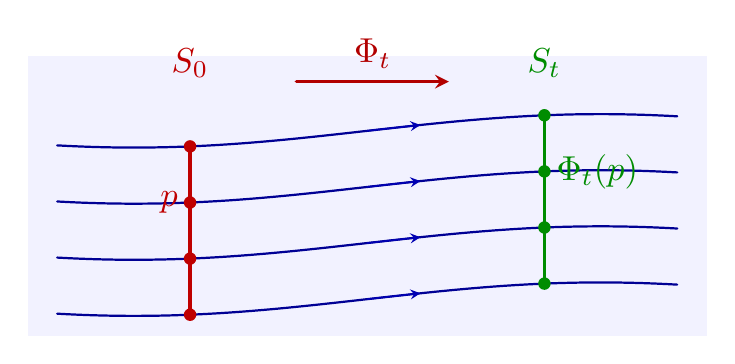
\begin{tikzpicture}[x=1cm,y=1cm,scale=1.25,transform shape,>=stealth,line cap=round]
  \fill[blue!5] (-3.45,-1.42) rectangle (3.45,1.42);
  \foreach \c in {-1.05,-.48,.09,.66}{
    \draw[blue!58!black,thick]
       plot[domain=-3.15:3.15,samples=55]
       ({\x},{\c+.17*sin(38*\x)});
    \draw[->,blue!70!black,semithick]
       (0,{\c}) -- (.54,{\c+.17*sin(38*.54)});
  }
  \draw[red!75!black,very thick]
      (-1.8,{-1.05+.17*sin(38*(-1.8))}) --
      (-1.8,{.66+.17*sin(38*(-1.8))});
  \draw[green!55!black,very thick]
      (1.8,{-1.05+.17*sin(38*1.8)}) --
      (1.8,{.66+.17*sin(38*1.8)});
  \foreach \c in {-1.05,-.48,.09,.66}{
    \fill[red!75!black] (-1.8,{\c+.17*sin(38*(-1.8))}) circle (1.8pt);
    \fill[green!55!black] (1.8,{\c+.17*sin(38*1.8)}) circle (1.8pt);
  }
  \node[red!75!black,above] at (-1.8,1.08) {$S_0$};
  \node[green!55!black,above] at (1.8,1.08) {$S_t$};
  \node[red!75!black,left] at (-1.8,{.09+.17*sin(38*(-1.8))}) {$p$};
  \node[green!55!black,right] at (1.8,{.09+.17*sin(38*1.8)}) {$\Phi_t(p)$};
  \draw[->,red!70!black,very thick]
      (-.72,1.16)--(.83,1.16) node[midway,above] {$\Phi_t$};
\end{tikzpicture}

\caption{Przepływ przesuwa przekrój poprzeczny $S_0$
na przekrój $S_t$, prowadząc każdy punkt wzdłuż jego krzywej
całkowej. Pokazane krzywe są trajektoriami pola
$X=(1,A\kappa\cos(\kappa x))$, gdzie $A=0.17$,
$\kappa=38\pi/180$. Jego przepływ ma postać
$\Phi_s(x,y)=(x+s,y+A[\sin(\kappa(x+s))-\sin(\kappa x)])$;
na rysunku $t=3.6$.}
\label{fig:przeplyw-przekroj}
\end{figure}

\begin{przyklad}[Trzy zupełne przepływy]
Na $\R^n$ pole stałe $X=v$ ma $\Phi_t(x)=x+tv$:
pochodna po $t$ jest równa $v$, niezależnie od położenia.
Pole Eulera $E=\sum_i x^i\partial_i$ ma $\Phi_t(x)=e^t x$,
bo $\frac{\dd}{\dd t}(e^t x)=e^t x=E_{e^t x}$.
Pole obrotowe z~\eqref{eq:obrot} ma
$\Phi_t(a,b)=(a\cos t-b\sin t,a\sin t+b\cos t)$.
Wszystkie trzy wzory są określone dla całego $t\in\R$ i
spełniają $\Phi_0=\id$ oraz $\Phi_{t+s}=\Phi_t\circ\Phi_s$.
\end{przyklad}

\begin{przyklad}[Ucieczka w skończonym czasie]\label{prz:niezupelne}
Dla $X=x^2\partial_x$ na $\R$ krzywa przez $x_0$ spełnia
$x'=x^2$, $x(0)=x_0$. Jeśli $x_0\ne0$, to przez krótki
czas $x(t)\ne0$, więc możemy zróżniczkować odwrotność:
$(1/x)'=-x'/x^2=-1$.
Całkowanie od $0$ do $t$ daje
$1/x(t)-1/x_0=-\int_0^t1\,\dd s=-t$.
Rozwiązując względem $x(t)$, dostajemy
\[
 \Phi_t(x_0)=\frac{x_0}{1-tx_0}
 \qquad\text{w maksymalnym przedziale zawierającym }0.
\]
Rzeczywiście, pochodna ilorazu wynosi
$x_0^2/(1-tx_0)^2=\Phi_t(x_0)^2$, a w chwili zero
otrzymujemy $x_0$. Dla $x_0=0$ ten sam wzór daje krzywą stałą.
Jeśli $x_0>0$, jej dziedzina to $(-\infty,1/x_0)$; jeśli $x_0<0$,
to $(1/x_0,\infty)$; dla $x_0=0$ jest nią $\R$.
Zatem dziedzina całego przepływu ma prosty opis
\[
\mathcal D_X=\{(t,x_0)\in\R^2:1-tx_0>0\}.
\]
Jest otwarta, ale nie jest iloczynem przedziału czasu i
całej prostej: czas, do którego dociera krzywa, zależy od $x_0$.
Dla ustalonego $t$ dziedziną $\Phi_t$ jest dokładnie
$M_t=\{x_0\in\R:1-tx_0>0\}$; dla $t=0$ jest to cała $\R$.
Algebraiczny wzór na $\Phi_t(x_0)$ ma też wartość przy
$1-tx_0<0$, lecz oddziela ją od chwili początkowej biegun
$t=1/x_0$; nie należy do tej samej krzywej całkowej.
Pole jest gładkie na całej prostej,
ale nie jest zupełne: nieograniczony wzrost rozwiązania powoduje
ucieczkę do nieskończoności w skończonym czasie.
\end{przyklad}

\begin{twierdzenie}[Kryterium przedłużenia i dwa warunki zupełności]
\label{thm:zupelnosc}
Jeśli maksymalna krzywa całkowa ma skończony prawy koniec $b$, to
opuszcza w pobliżu $b$ każdy zwarty podzbiór $M$.
W konsekwencji każde pole na rozmaitości zwartej jest zupełne.
Każde pole o zwartym nośniku na dowolnej rozmaitości także jest zupełne.
\end{twierdzenie}
\begin{proof}
\emph{Kryterium przedłużenia.}
Niech $I_p=(a,b)$ i $b<\infty$. Załóżmy przeciwnie,
że istnieją zbiór zwarty $K\subset M$ i ciąg
$t_j\nearrow b$ taki, że $\gamma_p(t_j)\in K$.
Po wybraniu podciągu mamy $\gamma_p(t_j)\to q\in K$.
Lokalne twierdzenie o istnieniu w $q$ daje otoczenie
$W\ni q$ i $\varepsilon>0$ takie, że z każdego punktu
$W$ można prowadzić rozwiązanie przez wszystkie czasy
$u\in(-\varepsilon,\varepsilon)$.
Dla dużego $j$ zachodzi $\gamma_p(t_j)\in W$
oraz $b-t_j<\varepsilon/2$.
Krzywa
\[
 u\longmapsto\Phi_u(\gamma_p(t_j)),\qquad
 -\varepsilon<u<\varepsilon,
\]
pokrywa się z $u\mapsto\gamma_p(t_j+u)$ w ich wspólnej
dziedzinie, bo obie zaczynają w $\gamma_p(t_j)$.
Możemy więc skleić je w krzywą określoną także dla
$t> b$, sprzecznie z maksymalnością $I_p$.
Przy skończonym lewym końcu stosujemy ten sam argument
do pola $-X$ i czasu odwróconego.

\emph{Zupełność na zbiorach zwartych.}
Jeśli $M$ jest zwarta, każda trajektoria przez cały czas
leży w jednym zwartym zbiorze $M$. Kryterium wyklucza
oba skończone końce $I_p$, zatem $I_p=\R$.
Teraz niech $K=\supp X$ będzie zwarty.
Jeśli $p\notin K$, to $X_p=0$, więc krzywa
stała w $p$ jest, z jednoznaczności, całą krzywą
maksymalną. Jeśli $p\in K$, krzywa nie może wejść
do $M\setminus K$: od chwili wejścia byłaby stała,
a jednoznaczność, zastosowana także wstecz w czasie,
zmusiłaby ją do bycia stałą już w chwili zero.
W obu przypadkach obraz $\gamma_p$ leży w zwartym
zbiorze $K\cup\{p\}$; kryterium znów daje $I_p=\R$.
\end{proof}

\begin{uwaga}[Nie mylić zupełności z brakiem zer]
Zupełne pole może mieć zera (obrót na płaszczyźnie), a pole bez zer
może być niezupełne, np.\ $X=(1+x^2)\partial_x$ na $\R$.
Dla rozmaitości z brzegiem pole musi dodatkowo być styczne do brzegu,
aby dać dwustronny przepływ zachowujący tę rozmaitość.
Istotnie, dyfeomorfizmy zachowują brzeg, więc różniczkowanie
krzywej $t\mapsto\Phi_t(p)$ dla $p\in\partial M$ daje
$X_p\in T_p\partial M$. Odwrotnie, dla pola stycznego do brzegu
rozwiązujemy równanie również na $\partial M$; jednoznaczność
w lokalnym przedłużeniu pola zapewnia, że jego krzywe przez
brzeg pozostają na brzegu. Krzywe z wnętrza nie mogą go
przekroczyć, bo przy pierwszym spotkaniu jednoznaczność wstecz
wymuszałaby wcześniejszy pobyt na brzegu.
Pole skierowane do wnętrza na brzegu daje zwykle przepływ tylko
dla małych dodatnich czasów, co wykorzystamy do budowania kołnierza.
Na przykład na $M=[0,\infty)$ pole $X=\partial_r$ jest gładkim
przekrojem pełnej wiązki stycznej, także w $0$.
Krzywa całkowa zaczynająca się w $0$ musiałaby mieć postać
$r(t)=t$, więc dla $t<0$ opuszczałaby $M$.
Nie ma tu sprzeczności ze Stwierdzeniem~\ref{prop:styczna-brzeg-1}:
$T_0M\cong\R$, ale $T_0\partial M=\{0\}$ i $X_0\notin T_0\partial M$.
Styczność do brzegu zapewnia lokalny przepływ dwustronny;
jego istnienie dla wszystkich czasów wymaga ponadto zupełności.
\end{uwaga}

\section{Geometria przepływu: prostowanie, niezmienniki, komutowanie}
\label{sec:prostowanie}

\begin{definicja}[Orbita i nasycenie przez przepływ]
\index{orbita i nasycenie przez przeplyw@Orbita i nasycenie przez przepływ}
\emph{Orbitą} punktu $p$ pod przepływem pola $X$ jest
$\mathcal O_X(p)=\{\Phi_t(p):t\in I_p\}$.
Dla $A\subseteq M$ jego \emph{nasycenie przez przepływ}
to suma orbit punktów z $A$:
\[
 \operatorname{Sat}_X(A)=\bigcup_{p\in A}\mathcal O_X(p).
\]
Zbiór $A$ jest \emph{nasycony przez $X$}, gdy
$\operatorname{Sat}_X(A)=A$, czyli gdy
$p\in A$ i $t\in I_p$ pociągają za sobą
$\Phi_t(p)\in A$.
\end{definicja}

To jest nasycenie względem relacji ,,leżeć na tej samej
orbicie'' w sensie Definicji~\ref{def:nasycenie}.
Istotnie, gdy $q=\Phi_s(p)$, to
$I_q=I_p-s$ i $\mathcal O_X(q)=\mathcal O_X(p)$
na mocy Twierdzenia~\ref{thm:przeplyw}; orbity rozcinają
więc $M$ na rozłączne klasy. Na przykład dla
$X=\partial_x$ na $\R^2$ nasyceniem
$\{0\}\times(0,1)$ jest cały pas $\R\times(0,1)$.

\begin{twierdzenie}[Twierdzenie o prostowaniu pola]\label{thm:flowbox}
Jeśli $X_p\ne0$, to istnieją współrzędne $(t,z^2,\ldots,z^n)$
w otoczeniu $p$, w których $X=\partial_t$. W tych współrzędnych
lokalny przepływ ma postać
\[
 (t,z^2,\ldots,z^n)\longmapsto(t+s,z^2,\ldots,z^n).
\]
\end{twierdzenie}
\begin{proof}
Wybieramy małą $(n-1)$-wymiarową podrozmaitość $S$
przechodzącą przez $p$ i poprzeczną do $X_p$, oraz parametryzację
$\sigma\colon V\subset\R^{n-1}\to S$ z $\sigma(0)=p$.
Można ją zbudować bez dodatkowego twierdzenia: wybieramy mapę
z $p=0$ i po liniowej zmianie współrzędnych z pierwszą składową
$X_p$ niezerową; bierzemy $S=\{x^1=0\}$ w tej mapie.
Odwzorowanie $F(t,z)=\Phi_t(\sigma(z))$ ma w $(0,0)$
różniczkę, której pierwszą kolumną jest $X_p$, a pozostałe kolumny
rozpinają $T_pS$. Jest więc izomorfizmem. Z twierdzenia o funkcji
odwrotnej $F$ jest lokalnym dyfeomorfizmem. Zmniejszamy jego
dziedzinę do produktu $(-\varepsilon,\varepsilon)\times V_0$.
Ponieważ $\partial_tF(t,z)=X_{F(t,z)}$, we współrzędnych $F^{-1}$
pole ma postać $\partial_t$. Prawo grupowe daje
$\Phi_s(F(t,z))=F(t+s,z)$, dopóki $t$ i $t+s$ leżą
w tym przedziale. To wyjaśnia lokalny zakres wzoru z tezy.
\end{proof}

Współrzędna $t$ mierzy czas ruchu od poprzecznego przekroju,
a $z=(z^2,\ldots,z^n)$ wskazuje punkt tego przekroju.
Gładką funkcję $h$ spełniającą $X(h)=0$ na otwartym zbiorze
\index{pierwsza calka@Pierwsza całka}
nazywamy tam \emph{całką pierwszą} pola: jej wartość nie zmienia się
wzdłuż żadnej trajektorii w tym zbiorze.
W prostującym otoczeniu trajektorie mają stałe $z$;
każda składowa $z^i$ jest więc lokalną całką pierwszą.

\begin{przyklad}[Jawne współrzędne prostujące]
Na $\R^2$ rozważmy pole
$X=\partial_x+y\partial_y$.
Jego krzywe całkowe spełniają $x'=1$, $y'=y$, więc
\[
\Phi_t(x_0,y_0)=(x_0+t,e^t y_0),
\qquad t\in\R.
\]
Jako przekrój poprzeczny wybieramy $S=\{x=0\}$ z
parametryzacją $\sigma(z)=(0,z)$.
Konstrukcja z dowodu Twierdzenia~\ref{thm:flowbox} daje
\[
F(t,z)=\Phi_t(\sigma(z))=(t,e^t z),
\qquad F^{-1}(x,y)=(x,e^{-x}y).
\]
W tym przykładzie $F$ jest dyfeomorfizmem całej $\R^2$,
więc prostowanie działa globalnie. Nowa współrzędna
$z=e^{-x}y$ nie zmienia się wzdłuż ruchu; bezpośrednio
\[
X(z)=\partial_x(e^{-x}y)+y\partial_y(e^{-x}y)
=-e^{-x}y+ye^{-x}=0.
\]
Orbity mają równania $y=Ce^x$, gdzie $C=z$ jest wartością
punktu przecięcia z $S$. Dla przedziału $(a,b)\subset\R$
nasycenie fragmentu przekroju jest zatem
\[
\operatorname{Sat}_X(\{0\}\times(a,b))
=\{(x,y)\in\R^2:a<e^{-x}y<b\}.
\]
Na Rysunku~\ref{fig:prostowanie-pola-przyklad} widać,
dlaczego współrzędna $z$ etykietuje trajektorie, a $t$
opisuje ruch po każdej z nich.
\end{przyklad}

\begin{figure}[!htbp]
\centering
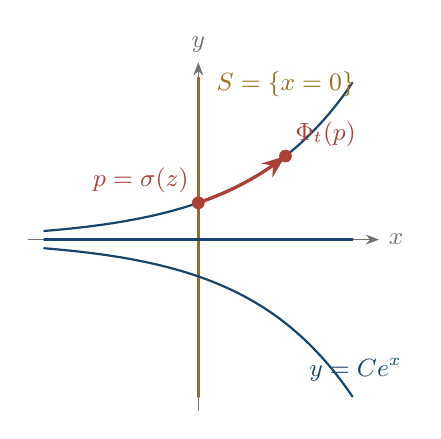
\begin{tikzpicture}[>=Stealth,x=1.35cm,y=.85cm,line cap=round]
  \draw[->,black!55] (-1.6,0)--(1.7,0) node[right,font=\small] {$x$};
  \draw[->,black!55] (0,-2.55)--(0,2.65) node[above,font=\small] {$y$};
  \draw[manifoldgold!75!black,very thick] (0,-2.35)--(0,2.42);
  \foreach \c in {-.55,0,.55}{
    \draw[manifoldblue!75!black,thick]
      plot[domain=-1.45:1.45,samples=60] (\x,{\c*exp(\x)});
  }
  \draw[->,manifoldred,very thick]
    plot[domain=0:.82,samples=35] (\x,{.55*exp(\x)});
  \fill[manifoldred] (0,.55) circle (2.3pt)
    node[above left,font=\small] {$p=\sigma(z)$};
  \fill[manifoldred] (.82,{.55*exp(.82)}) circle (2.3pt)
    node[above right,font=\small] {$\Phi_t(p)$};
  \node[manifoldgold!75!black,font=\small,anchor=west]
    at (.08,2.32) {$S=\{x=0\}$};
  \node[manifoldblue!75!black,font=\small] at (1.48,-1.95)
    {$y=Ce^x$};
\end{tikzpicture}
\caption{Pole $X=\partial_x+y\partial_y$: niebieskie krzywe są
orbitami $y=Ce^x$. Każda przecina złoty przekrój $S$ w jednym
punkcie $(0,C)$. Czerwony łuk pokazuje ruch od $p$ do $\Phi_t(p)$;
współrzędna $z=C$ pozostaje na nim stała.}
\label{fig:prostowanie-pola-przyklad}
\end{figure}

\begin{uwaga}
Pola nie można wyprostować w zerze $X_p=0$: dyfeomorfizm przenosi
wektor zerowy na wektor zerowy, natomiast $\partial_t$ nigdzie
nie znika. W zerze lokalne trajektorie i zachowanie przepływu
bada się innymi metodami niż prostowanie pola.
\end{uwaga}

\begin{stwierdzenie}[Lokalne twierdzenie Frobeniusa]
\label{prop:frobenius-lokalny}
Gładki rozkład inwolutywny $\mathcal D$ stałego rzędu $k$
ma lokalnie współrzędne, w których jest rozpięty przez pierwsze
$k$ pól współrzędnych.
\end{stwierdzenie}
\begin{proof}
Przeprowadzimy indukcję po $k$, jednocześnie dla wszystkich
wymiarów rozmaitości. Dla $k=0$ teza jest natychmiastowa.
Dla $k\ge1$ wybieramy lokalną bazę $X_1,\ldots,X_k$ rozkładu
i prostujemy niezerowe $X_1$. Mamy więc współrzędne $(t,z)$
w produkcie wokół $(0,0)$, z $X_1=\partial_t$.
Od każdego $X_j$, $j\ge2$, odejmujemy jego składową w kierunku
$\partial_t$. Otrzymane pola $Y_2,\ldots,Y_k$ nie mają tej
składowej, a wraz z $\partial_t$ nadal stanowią bazę $\mathcal D$.
Jeśli $k=1$, dowód jest już zakończony.

Niech $B(t,z)$ będzie macierzą o $k-1$ kolumnach złożonych
ze składowych $Y_2,\ldots,Y_k$ w kierunkach $z$.
Inwolutywność daje $[\partial_t,Y_j]\in\mathcal D$;
ponieważ ten nawias nie ma składowej czasowej, jest kombinacją
samych $Y_2,\ldots,Y_k$. Zatem
\[
 \partial_tB(t,z)=B(t,z)A(t,z)
\]
dla pewnej gładkiej macierzy kwadratowej $A$.
Gładkość współczynników wynika z rozwiązania układu za pomocą
niezerowego minora macierzy $B$, po zmniejszeniu otoczenia.
Rozwiązujemy macierzowe równanie
\[
 \partial_tQ(t,z)=-A(t,z)Q(t,z),\qquad Q(0,z)=I.
\]
Istnienie i gładka zależność od $z$ wynikają z
Twierdzenia~\ref{thm:ode}: dołączamy zmienne z równaniami
$t'=1$, $z'=0$. Po zmniejszeniu produktu $Q$ jest odwracalna,
bo $Q(0,0)=I$. Reguła iloczynu daje
\[
 \partial_t(BQ)=BAQ-BAQ=0,\qquad B(t,z)Q(t,z)=B(0,z).
\]
Kolumny $BQ$ wyznaczają więc nową bazę pól pionowych
niezależnych od $t$, rozpinającą te same kierunki co kolumny $B$.
Na przekroju $t=0$ tworzą rozkład rzędu $k-1$.
Jest on inwolutywny: nawiasy tych pól nie mają składowej
czasowej, należą do $\mathcal D$ i nie zależą od $t$;
reguła Leibniza dla nawiasu rozszerza to na dowolne sekcje.
Z założenia indukcyjnego istnieje zmiana współrzędnych $z$
prostująca ten rozkład. Stosujemy ją niezależnie od $t$.
Ponieważ baza pionowa nie zależy od czasu, w całym produkcie
$\mathcal D$ jest rozpięty przez $\partial_t$ i pierwsze
$k-1$ nowych pól współrzędnych na przekroju. To kończy indukcję.
\end{proof}

\begin{stwierdzenie}[Funkcje i pola niezmiennicze]\label{prop:inwarianty}
Dla zupełnego $X$ gładka funkcja $f\in C^\infty(M)$ jest stała na każdej jego trajektorii
wtedy i tylko wtedy, gdy $X(f)=0$. Przepływ zawsze zachowuje
pole, które go generuje: $(\Phi_t)_*X=X$.
Dla innego pola $Y$ następujące warunki są równoważne:
\begin{enumerate}[label=(\roman*)]
\item $[X,Y]=0$;
\item $(\Phi_t)_*Y=Y$ dla wszystkich $t$;
\item dla każdego $p\in M$ i $t\in\R$ zachodzi
$I^Y_{\Phi_t^X(p)}=I^Y_p$ oraz
$\Phi_t^X(\Phi_s^Y(p))=\Phi_s^Y(\Phi_t^X(p))$
dla każdego $s\in I^Y_p$.
\end{enumerate}
Jeśli także $Y$ jest zupełne, ostatni punkt oznacza
$\Phi_t^X\circ\Phi_s^Y=\Phi_s^Y\circ\Phi_t^X$ dla wszystkich $s,t\in\R$.
\end{stwierdzenie}
\begin{proof}
Reguła łańcucha daje
$\frac{\dd}{\dd t}f(\Phi_t(p))=X(f)(\Phi_t(p))$.
Jeśli $X(f)=0$, funkcja czasu jest stała na $\R$;
odwrotnie, stałość każdej trajektorii daje pochodną zerową w $t=0$.
Druga równość wynika z~\eqref{eq:przeplyw-generuje}.

Wykażmy (i)$\Leftrightarrow$(ii) bez porównywania wektorów
z różnych przestrzeni stycznych. Ustalmy $p$ i oznaczmy
$\gamma(t)=\Phi_t^X(p)$. Na krótkim fragmencie krzywej
w jednej mapie traktujemy pola jako funkcje o wartościach w $\R^n$.
Oznaczmy tam
\[
V(t)=(\dd\Phi_t^X)_pY_p,
\qquad W(t)=Y_{\gamma(t)}.
\]
Równanie wariacyjne z dowodu Twierdzenia~\ref{thm:ode}
daje $V'(t)=\D X(\gamma(t))V(t)$.
Reguła łańcucha daje natomiast
$W'(t)=\D Y(\gamma(t))X_{\gamma(t)}$.
W tych samych współrzędnych wzór~\eqref{eq:nawias-wspolrzedne}
przyjmuje postać $[X,Y]=\D Y\,X-\D X\,Y$.
Jeśli (i) zachodzi, to $W'=\D X(\gamma)W$.
Ponieważ $V(0)=W(0)=Y_p$, jednoznaczność liniowego ODE
daje $V=W$ na pierwszym fragmencie. Na jego końcu są one
tym samym wektorem w $T_{\gamma(t)}M$, więc stanowią wspólną
wartość początkową po przejściu do następnej mapy.
Skończone pokrycie każdego zwartego odcinka czasu pozwala
powtórzyć argument aż do dowolnego $t$. Dostajemy
$(\dd\Phi_t^X)_pY_p=Y_{\Phi_t^X(p)}$ dla każdego $t$,
czyli (ii). Odwrotnie, przy (ii) mamy $V=W$;
porównanie ich pochodnych w $t=0$ daje
$\D X(p)Y_p=\D Y(p)X_p$, a więc $[X,Y]_p=0$.

Niech $\Psi_s$ oznacza maksymalny przepływ $Y$. Przy (ii)
dla każdego ustalonego $t$ krzywa $s\mapsto\Phi_t(\Psi_s(p))$
ma pochodną $\dd\Phi_t(Y)=Y$ i zaczyna w $\Phi_t(p)$.
Jednoznaczność i maksymalność dają
$I_p^Y\subseteq I_{\Phi_t(p)}^Y$ oraz
$\Phi_t(\Psi_s(p))=\Psi_s(\Phi_t(p))$ dla $s\in I_p^Y$.
Ponieważ $\Phi_t$ jest globalnym dyfeomorfizmem, zastosowanie
tego samego argumentu do $\Phi_{-t}$ daje odwrotne zawieranie
przedziałów. Otrzymaliśmy więc (iii) wraz ze zgodnością dziedzin.
Różniczkując (iii) po $s$ w zerze, odzyskujemy
$\dd\Phi_t(Y_p)=Y_{\Phi_t(p)}$, czyli (ii).
\end{proof}

Przy niezupełnym $X$ równości o zachowaniu pola i komutowaniu
pozostają lokalne: stosujemy je na wspólnej dziedzinie, na której
wszystkie występujące przepływy i ich złożenia są określone.

\begin{przyklad}[Dwa komutujące przepływy]
Wróćmy do $X=\partial_x+y\partial_y$ z przykładu prostowania
i weźmy $Y=y\partial_y$ na $\R^2$.
Współrzędnościowy wzór na nawias daje
\[
[X,Y]=[\partial_x+y\partial_y,y\partial_y]
=\bigl(X(y)-Y(y)\bigr)\partial_y=0.
\]
Przepływ $Y$ ma postać $\Psi_s(x,y)=(x,e^s y)$ i jest zupełny.
Oba złożenia można obliczyć bezpośrednio:
\[
\Phi_t(\Psi_s(x,y))=(x+t,e^{t+s}y)
=\Psi_s(\Phi_t(x,y)).
\]
W prostujących współrzędnych $(t,z)=(x,e^{-x}y)$
pole $Y$ ma współczynniki $Y(t)=y\partial_yx=0$
i $Y(z)=y\partial_y(e^{-x}y)=e^{-x}y=z$.
Zatem pole $X$ przesuwa tylko $t$, a $Y=z\partial_z$ zmienia
tylko $z$; stąd ich ruchy mają niezależne kierunki.
\end{przyklad}

\begin{przyklad}[Pierwsza całka]
Dla pola obrotowego $R=-y\partial_x+x\partial_y$
funkcja $f(x,y)=x^2+y^2$ spełnia
$R(f)=(-y)(2x)+x(2y)=0$.
Jej dodatnie poziomice są okręgami, po których biegnie przepływ;
poziomica zerowa to nieruchomy punkt $(0,0)$, a ujemne są puste.
Jest to globalna pierwsza całka pola obrotowego.
W ogólności poziomica pierwszej całki może zawierać kilka orbit:
dla $X=\partial_x$ na $\R^2$ funkcja $h(x,y)=y^2$ spełnia
$X(h)=0$, lecz poziomica $h^{-1}(1)$ składa się z dwóch
oddzielnych orbit $y=1$ i $y=-1$.
\end{przyklad}

\section{Pochodna Liego: porównywanie danych w różnych punktach}
\label{sec:liego}

Nie można po prostu odjąć wektorów $Y_{\Phi_t(p)}$ i $Y_p$:
należą do różnych przestrzeni stycznych. Przepływ $X$ dostarcza
\emph{kanonicznego w tej sytuacji} sposobu ich porównania:
różniczka odwrotnego przepływu przenosi pierwszy z nich do $T_pM$.
Otrzymujemy odpowiedź na pytanie, jak obiekt zmienia się
wraz z ruchem generowanym przez $X$.

\begin{definicja}\label{def:pochodna-liego}
\index{pochodna Liego@Pochodna Liego}
Dla funkcji $f$ i pola $Y$ określamy
\begin{align}
 (\Lie_Xf)(p)
 &=\left.\frac{\dd}{\dd t}\right|_{0}f(\Phi_t(p))=X(f)(p),
 \label{eq:lie-f}\\
 (\Lie_XY)_p
 &=\left.\frac{\dd}{\dd t}\right|_{0}
 (\dd\Phi_{-t})_{\Phi_t(p)}Y_{\Phi_t(p)}.
 \label{eq:lie-y}
\end{align}
Definicja jest lokalna: przepływ jest potrzebny tylko dla małego $t$.
Wzór~\eqref{eq:lie-y} zapisujemy krótko jako
$\Lie_XY=\left.\frac{\dd}{\dd t}\right|_0\Phi_t^*Y$.
\end{definicja}


\begin{figure}[!htbp]
\centering
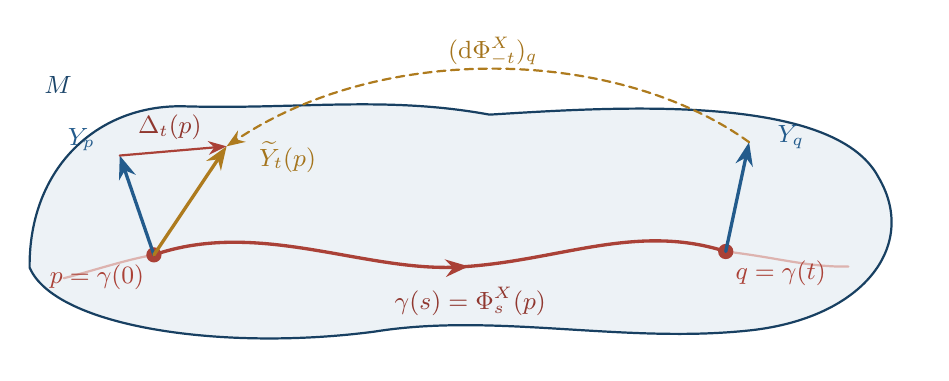
\begin{tikzpicture}[>=Stealth,scale=1.06,line cap=round,line join=round]
% Jedno spójne otoczenie na M; p i q są punktami czerwonej trajektorii.
\filldraw[fill=manifoldblue!8,draw=manifoldblue!70!black,thick]
 (-5.14,-.67) .. controls (-5.15,.52) and (-4.33,1.28) .. (-3.3,1.26)
 .. controls (-1.92,1.22) and (-.88,1.39) .. (.37,1.16)
 .. controls (1.84,1.25) and (4.49,1.43) .. (5.03,.41)
 .. controls (5.52,-.42) and (4.83,-1.3) .. (3.44,-1.43)
 .. controls (1.94,-1.58) and (.42,-1.21) .. (-1.01,-1.44)
 .. controls (-2.84,-1.68) and (-4.84,-1.38) .. cycle;
\node[font=\small,manifoldblue!75!black] at (-4.8,1.51) {$M$};
\coordinate (P) at (-3.65,-.52);
\coordinate (Q) at (3.2,-.48);
% Ciągła krzywa całkowa; wyraźne punkty p, q i kierunek czasu.
\draw[manifoldred!40,thick] (-4.73,-.8)
 .. controls (-4.38,-.71) and (-3.96,-.57) .. (P);
\draw[manifoldred,very thick,postaction={decorate},
 decoration={markings,mark=at position .55 with {\arrow{Stealth}}}]
 (P) .. controls (-2.43,-.1) and (-1.21,-.69) .. (-.1,-.67)
 .. controls (1.13,-.63) and (2.08,-.12) .. (Q);
\draw[manifoldred!40,thick] (Q)
 .. controls (3.81,-.55) and (4.19,-.67) .. (4.67,-.66);
\node[font=\small,manifoldred!85!black] at (.14,-1.08)
 {$\gamma(s)=\Phi_s^X(p)$};
\fill[manifoldred] (P) circle (2.6pt)
 node[below left,font=\small] {$p=\gamma(0)$};
\fill[manifoldred] (Q) circle (2.6pt)
 node[below right,font=\small] {$q=\gamma(t)$};
% Wektory porównywane po sprowadzeniu do T_p M.
\draw[->,manifoldblue,very thick] (P)--(-4.06,.67);
\draw[->,manifoldgold!85!black,very thick] (P)--(-2.78,.78);
\node[font=\small,manifoldblue] at (-4.52,.86) {$Y_p$};
\node[font=\small,manifoldgold!80!black] at (-2.05,.65)
 {$\widetilde Y_t(p)$};
\draw[->,manifoldred,thick] (-4.06,.67)--(-2.78,.78);
\node[font=\small,manifoldred!85!black] at (-3.46,1.01) {$\Delta_t(p)$};
% Wektor Y_q oraz schemat cofnięcia jego wartości, odrębny od trajektorii.
\draw[->,manifoldblue,very thick] (Q)--(3.48,.83);
\node[font=\small,manifoldblue] at (3.98,.89) {$Y_q$};
\draw[->,manifoldgold!85!black,thick,densely dashed]
 (3.48,.83) .. controls (1.93,1.95) and (-.88,2.05) .. (-2.78,.78);
\node[font=\small,manifoldgold!80!black] at (.41,1.92)
 {$(\dd\Phi_{-t}^X)_q$};
\end{tikzpicture}
\caption{Punkty $p=\gamma(0)$ i $q=\gamma(t)=\Phi_t^X(p)$ leżą
na tej samej krzywej całkowej na $M$; czerwona strzałka pokazuje
ruch w czasie od $p$ do $q$. Wektor $Y_q$ cofamy różniczką
przepływu do $T_pM$, otrzymując $\widetilde Y_t(p)$.
Tam porównujemy go z $Y_p$; $\Delta_t(p)$ jest ich różnicą.
Przerywana strzałka przedstawia transport wektora, nie ruch punktu.}
\label{fig:pochodna-liego}
\end{figure}

Dokładnie, oznaczając $q=\Phi_t^X(p)$, mamy
\[
 \widetilde Y_t(p):=(\dd\Phi_{-t}^X)_qY_q\in T_pM,\qquad
 (\Lie_XY)_p=\lim_{t\to0}\frac{\widetilde Y_t(p)-Y_p}{t}.
\]
Dla każdego małego $t$ oba odejmowane wektory leżą w $T_pM$.
Rysunek~\ref{fig:pochodna-liego} pokazuje różnicę $\Delta_t(p)$,
której iloraz przez $t$ ma granicę dla $t\to0$.


\begin{twierdzenie}\label{thm:lie-nawias}
Dla dowolnych pól $X,Y$ zachodzi
\begin{equation}\label{eq:lie-nawias}
 \Lie_XY=[X,Y].
\end{equation}
Zatem pochodna Liego funkcji jest działaniem derywacji,
a pochodna Liego pola jest nawiasem.
\end{twierdzenie}
\begin{proof}
Ustalmy $p\in M$ i $f\in C^\infty(M)$. Pracujemy w otoczeniu $p$
i dla na tyle małych $|t|$, aby lokalny przepływ $\Phi_t=\Phi_t^X$
oraz $\Phi_{-t}$ były określone we wszystkich rozważanych punktach.
Z definicji cofnięcia pola, przy $q=\Phi_t(p)$,
\[
 Z_t(p):=(\Phi_t^*Y)_p=(\dd\Phi_{-t})_qY_q\in T_pM.
\]
Wektory $Z_t(p)$ leżą więc w \emph{jednej} przestrzeni $T_pM$,
a $Z_0(p)=Y_p$. Aby obliczyć ich pochodną, zadziałajmy nimi
na dowolną funkcję $f$. Definicja różniczki daje
\begin{equation}\label{eq:lie-pullback-funkcja}
 Z_t(p)(f)
 =Y_q(f\circ\Phi_{-t})
 =Y(f\circ\Phi_{-t})(\Phi_t(p)).
\end{equation}
Oznaczmy $F(t,r):=f(\Phi_{-t}(r))$ dla $r$ w otoczeniu $p$.
Ponieważ $\frac{\dd}{\dd t}\Phi_{-t}(r)=-X_{\Phi_{-t}(r)}$,
reguła łańcucha daje
\[
 F(0,r)=f(r),\qquad
 \left.\frac{\partial F}{\partial t}\right|_{(0,r)}
 =-X(f)(r).
\]
Niech $H(t,r):=Y_r(F(t,\cdot))$. Wtedy prawa strona
\eqref{eq:lie-pullback-funkcja} jest równa $H(t,\Phi_t(p))$.
Różniczkując to złożenie, musimy uwzględnić zarówno zmianę
funkcji $H$ z czasem, jak i ruch punktu $\Phi_t(p)$:
\begin{align*}
 \left.\frac{\dd}{\dd t}H(t,\Phi_t(p))\right|_{t=0}
 &=\left.\frac{\partial H}{\partial t}\right|_{(0,p)}
   +X_p\bigl(H(0,\cdot)\bigr) \\
 &=-Y_p\bigl(X(f)\bigr)+X_p\bigl(Y(f)\bigr).
\end{align*}
W drugim kroku użyliśmy $H(0,\cdot)=Y(f)$ oraz
$\partial_tH(0,p)=Y_p\bigl(\partial_tF(0,\cdot)\bigr)$.
Zamiana kolejności $Y$ i $\partial_t$ jest dopuszczalna:
w lokalnych współrzędnych $Y=\sum_iY^i(r)\partial_{r^i}$,
współczynniki $Y^i$ nie zależą od $t$, a funkcja $F$ jest gładka.
Wreszcie, ponieważ $Z_t(p)$ jest gładką krzywą w $T_pM$,
jej pochodną można obliczyć po przyłożeniu do $f$. Otrzymujemy
\[
 (\Lie_XY)_p(f)
 =\left.\frac{\dd}{\dd t}Z_t(p)(f)\right|_{t=0}
 =X(Yf)(p)-Y(Xf)(p)=[X,Y]_p(f).
\]
Równość zachodzi dla każdej funkcji gładkiej $f$. Funkcje gładkie
rozróżniają wektory styczne: wystarczy wziąć funkcje, które
w pobliżu $p$ pokrywają się ze współrzędnymi lokalnymi.
Zatem $(\Lie_XY)_p=[X,Y]_p$; punkt $p$ był dowolny.
\end{proof}

\begin{stwierdzenie}\label{prop:lie-ewolucja}
Na wspólnych dziedzinach lokalnego przepływu pola $X$ zachodzi
\[
 \frac{\dd}{\dd t}\Phi_t^*Y=\Phi_t^*[X,Y].
\]
\end{stwierdzenie}
\begin{proof}
Dla dyfeomorfizmu $F$ cofnięcie pola oznacza $F^*Y=(F^{-1})_*Y$.
Reguła łańcucha daje $(F\circ G)^*=G^*\circ F^*$.
Prawo grupowe przepływu pozwala zatem napisać
$\Phi_{t+h}^*Y=\Phi_t^*(\Phi_h^*Y)$.
Ustalamy punkt i dostatecznie małe wspólne otoczenie, aby
wszystkie te odwzorowania były określone dla $h$ bliskiego zeru.
Różniczkujemy po $h$ w zerze: liniowe odwzorowanie cofające przez
ustalone $\Phi_t$ nie zależy od $h$, a
$\left.\partial_h\right|_0\Phi_h^*Y=[X,Y]$
na mocy Twierdzenia~\ref{thm:lie-nawias}.
\end{proof}

\begin{uwaga}[Ten sam rachunek we współrzędnych]
W lokalnych współrzędnych, zapisując pola jako kolumny funkcji,
gładkość przepływu daje przy $t\to0$
\[
 \Phi_t(x)=x+tX(x)+o(t),\qquad
 \dd\Phi_t|_x=I+t\,\dd X|_x+o(t),
\]
ponieważ $\partial_t\Phi_t|_{t=0}=X$,
a gładkość łączna pozwala zamienić pochodne:
$\partial_t(\dd\Phi_t)|_{t=0}
=\dd(\partial_t\Phi_t|_{t=0})=\dd X$.
Wyjaśnijmy też znak w różniczce odwrotnej.
Dla $J_t=\dd\Phi_t|_x=I+t\,\dd X|_x+o(t)$
mamy $J_t^{-1}\to I$ oraz
\[
 J_t^{-1}-I=-J_t^{-1}(J_t-I)
 =-J_t^{-1}\bigl(t\,\dd X|_x+o(t)\bigr)
 =-t\,\dd X|_x+o(t).
\]
Różniczkując $\Phi_{-t}\circ\Phi_t=\id$, dostajemy więc
$\dd\Phi_{-t}|_{\Phi_t(x)}=J_t^{-1}
=I-t\,\dd X|_x+o(t)$ oraz
$Y(\Phi_t(x))=Y(x)+t\,\dd Y|_xX(x)+o(t)$.
Po pomnożeniu obu wyrażeń otrzymujemy
\[
 (\Phi_t^*Y)(x)=Y(x)+t\bigl(\dd Y|_xX(x)-\dd X|_xY(x)\bigr)+o(t).
\]
Zatem składowa $j$ pochodnej wynosi
$\sum_i(X^i\partial_iY^j-Y^i\partial_iX^j)$,
co zgadza się ze wzorem na nawias Liego.
\end{uwaga}

\begin{przyklad}[Obliczenie w polu przesunięć]
Dla $X=\partial_x$ i $Y=x\partial_y$ mamy
$\Phi_t(x,y)=(x+t,y)$. W punkcie $q=(x+t,y)$ jest
$Y_q=(x+t)\partial_y$, a cofająca różniczka przesunięcia
działa identycznościowo na wektory. Zatem
\[
 ((\Phi_t)^*Y)_{(x,y)}=(x+t)\partial_y,
 \qquad \Lie_XY=\partial_y.
\]
Nie chodzi o różnicę położeń punktów, tylko o zmianę pola
po przeniesieniu obu wektorów do tej samej przestrzeni stycznej.
\end{przyklad}

\begin{przyklad}[Transport przez skalowanie]
Na $\R$ niech $X=x\partial_x$ oraz $Y=\partial_x$.
Przepływ $X$ ma postać $\Phi_t(x)=e^t x$.
W punkcie $q=e^t x$ wartość pola $Y_q$ ma współczynnik $1$,
ale różniczka powrotnego przepływu mnoży wektor przez $e^{-t}$.
Stąd
\[
(\Phi_t^*Y)_x=(\dd\Phi_{-t})_qY_q=e^{-t}\partial_x\big|_x,
\qquad \Lie_XY=-\partial_x.
\]
Ten sam wynik daje nawias:
$[x\partial_x,\partial_x](f)=xf''-(f'+xf'')=-f'$.
Współczynnik $Y$ jest stały, więc cała zmiana pochodzi tu z
transportu wektora przez różniczkę $\Phi_{-t}$.
\end{przyklad}

\begin{figure}[!htbp]
\centering
\begin{tikzpicture}[>=Stealth,scale=1.12,line cap=round,line join=round]
% Cztery kroki komutatora dla X=\partial_x, Y=(1+x)\partial_y.
\coordinate (P) at (-2,-.68);
\coordinate (A) at (.7,-.68);
\coordinate (B) at (.7,1.04);
\coordinate (C) at (-2,1.04);
\coordinate (Q) at (-2,.04);
\fill[manifoldblue!5] (-2.65,-1.15) rectangle (1.38,1.52);
\draw[manifoldblue!22,thin] (-2.65,-1.15) rectangle (1.38,1.52);
\draw[->,very thick,manifoldblue] (P)--(A)
 node[midway,below,font=\small] {$\Phi_t^X$};
\draw[->,very thick,manifoldgreen] (A)--(B)
 node[midway,right,font=\small] {$\Phi_t^Y$};
\draw[->,very thick,manifoldblue] (B)--(C)
 node[midway,above,font=\small] {$\Phi_{-t}^X$};
\draw[->,very thick,manifoldgreen] (C)--(Q)
 node[midway,left,font=\small] {$\Phi_{-t}^Y$};
\fill[manifoldred] (P) circle (2.5pt) node[below left,font=\small] {$p$};
\fill[manifoldred] (Q) circle (2.5pt) node[left,font=\small] {$C_t(p)$};
\draw[->,thick,manifoldred,densely dashed] (-1.66,-.68)--(-1.66,.04)
 node[midway,right,font=\small] {$t^2[X,Y]_p$};
\node[font=\footnotesize,align=center] at (3.7,.52)
 {$C_t=\Phi_{-t}^Y\circ\Phi_{-t}^X$\\[2pt]
 $\circ\Phi_t^Y\circ\Phi_t^X$};
\node[font=\footnotesize,align=center,text width=3.4cm] at (3.75,-.6)
 {Końcowy punkt leży o rząd $t^2$ ponad początkiem.};
\end{tikzpicture}
\caption{Komutator małych przepływów. Po przejściu kolejno wzdłuż
$X,Y,-X,-Y$ droga zwykle się nie zamyka; wyraz przemieszczenia rzędu $t^2$ jest wyznaczony przez nawias
$[X,Y]$. Jeśli $[X,Y]_p=0$, wyraz rzędu $t^2$ znika;
ewentualny pierwszy niezerowy wyraz ma wyższy rząd.
Rysunek schematycznie ilustruje przykład
$X=\partial_x$, $Y=(1+x)\partial_y$.}
\label{fig:komutator-przeplywow}
\end{figure}

Jeśli $C_t=\Phi_{-t}^Y\circ\Phi_{-t}^X\circ\Phi_t^Y\circ\Phi_t^X$, to
w dowolnej mapie wokół $p$ (i dla małego $t$)
\[
 x(C_t(p))=x(p)+t^2\,\dd x_p([X,Y]_p)+O(t^3).
\]
W przykładzie $X=\partial_x$, $Y=(1+x)\partial_y$ i $p=(0,0)$
można to policzyć dokładnie: $p\to(t,0)\to(t,t+t^2)
\to(0,t+t^2)\to(0,t^2)$. Geometria rysunku zgadza się więc ze
znakiem konwencji~\eqref{eq:nawias-def}.

Uzasadnijmy także wzór ogólny, zamiast wnioskować z jednego przykładu.
W ustalonej mapie przepływ gładkiego pola $Z$ ma rozwinięcie
\[
 \Phi_t^Z(x)=x+tZ(x)+\tfrac12t^2 DZ(x)Z(x)+O(t^3),
\]
bo druga pochodna krzywej całkowej w zerze to $DZ(x)Z(x)$.
Oznaczmy kolejne punkty czterech kroków przez $x_1,\ldots,x_4$.
Wstawiamy to rozwinięcie kolejno do
$x_1=\Phi_t^X(x)$, $x_2=\Phi_t^Y(x_1)$,
$x_3=\Phi_{-t}^X(x_2)$ i $x_4=\Phi_{-t}^Y(x_3)$.
Przy rozwijaniu pól w punktach pośrednich potrzebne są
\[
 \begin{aligned}
 Y(x_1)&=Y(x)+t\,DY(x)X(x)+O(t^2),\\
 X(x_2)&=X(x)+t\,DX(x)(X(x)+Y(x))+O(t^2),\\
 Y(x_3)&=Y(x)+t\,DY(x)Y(x)+O(t^2).
 \end{aligned}
\]
Każda z tych równości to wzór Taylora pierwszego rzędu:
używamy kolejno $x_1-x=tX+O(t^2)$,
$x_2-x=t(X+Y)+O(t^2)$ i $x_3-x=tY+O(t^2)$.
Wyrazy kwadratowe samych przepływów można liczyć w $x$,
bo przesunięcie argumentu o $O(t)$ zmienia je dopiero o $O(t^3)$.
Po podstawieniu i zebraniu potęg dostajemy
\begin{align*}
 x_1&=x+tX+\tfrac12t^2 DX\,X+O(t^3),\\
 x_2&=x+t(X+Y)+t^2(\tfrac12 DX\,X+DY\,X+\tfrac12 DY\,Y)+O(t^3),\\
 x_3&=x+tY+t^2(DY\,X+\tfrac12 DY\,Y-DX\,Y)+O(t^3),\\
 x_4&=x+t^2(DY\,X-DX\,Y)+O(t^3).
\end{align*}
Wszystkie pola i ich macierze pochodnych po prawej stronie
są obliczone w $x$. Równość $DY\,X-DX\,Y=[X,Y](x)$
wynika ze wzoru~\eqref{eq:nawias-wspolrzedne}.
Reszty $O(t^3)$ są rozumiane w tej mapie, dla punktów w
dostatecznie małym otoczeniu i małego czasu, gdy złożenia istnieją.
Drugi wiersz tabeli wyjaśnia również wcześniejsze porównanie
kolejności dwóch ruchów z Sekcji~\ref{sec:nawias}.
Po zamianie $X$ z $Y$ zmienia się w nim tylko składnik
$DY\,X$ na $DX\,Y$. Dlatego współrzędne końców ruchów
$X,Y$ i $Y,X$ różnią się o $t^2(DY\,X-DX\,Y)+O(t^3)$.


\begin{uwaga}[Znaczenie znaku]
W~\eqref{eq:lie-y} wektor cofamy przez $\Phi_{-t}$.
Niech $q=\Phi_t(p)$. Oba wektory $Y_q$ i
$(\dd\Phi_t)_pY_p$ należą do $T_qM$, a ich różnicę
możemy cofnąć do $T_pM$:
\[
(\dd\Phi_{-t})_q\bigl(Y_q-(\dd\Phi_t)_pY_p\bigr)
=(\Phi_t^*Y)_p-Y_p.
\]
Pochodna tego wyrażenia w $t=0$ jest równa
$[X,Y]_p$; odwrócenie kolejności odejmowania zmienia znak.
W przykładzie $X=\partial_x$, $Y=x\partial_y$ różnica
$Y_{\Phi_t(p)}-(\dd\Phi_t)_pY_p$ wynosi $t\partial_y$,
zgodnie z dodatnim znakiem $[X,Y]=\partial_y$.
\end{uwaga}

\section{Pola zależne od czasu i izotopie}
\label{sec:izotopie}

Przepływ pola stałego w czasie spełnia lokalne prawo grupowe;
dla pola zupełnego tworzy jednoparametrową grupę dyfeomorfizmów.
W topologii różniczkowej często trzeba deformować obiekty według
zaplanowanego ruchu, którego prędkość może zmieniać się z czasem.

\begin{definicja}
\emph{Pole zależne od czasu} to rodzina $X_t\in\X(M)$,
$t\in[0,1]$, gładka łącznie w $(t,p)$ (na końcach przedziału
w sensie lokalnego gładkiego przedłużenia). Jej krzywe całkowe spełniają nieautonomiczne równanie
$\gamma'(t)=(X_t)_{\gamma(t)}$. Odwzorowanie ewolucji
$F_{t,s}(p)$ przenosi położenie w chwili $s$ do położenia
w chwili $t$, tam gdzie rozwiązanie istnieje.
\end{definicja}

Dodanie czasu jako zmiennej sprowadza to równanie do autonomicznego
pola $\widehat X=\partial_t+X_t$ na czasoprzestrzeni.
Krzywa tego pola startująca w $(s,p)$ ma postać
$(s+u,F_{s+u,s}(p))$. Twierdzenie~\ref{thm:ode}, zastosowane
lokalnie także do przedłużeń przy końcach przedziału, daje
gładkość ewolucji łącznie w $(t,s,p)$. Jednoznaczność daje prawo
\begin{equation}\label{eq:ewolucja}
 F_{s,s}=\id,\qquad F_{u,t}\circ F_{t,s}=F_{u,s},
 \qquad F_{s,t}=F_{t,s}^{-1}.
\end{equation}
Równości obowiązują tam, gdzie odpowiednie rozwiązania istnieją;
$F_{t,s}$ jest dyfeomorfizmem swojej otwartej dziedziny na obraz,
z odwrotnością $F_{s,t}$.
Zwykle $F_{t,0}$ \emph{nie} spełnia
$F_{t+s,0}=F_{t,0}\circ F_{s,0}$, bo samo pole się zmienia.
Jeżeli nośniki wszystkich $X_t$ mieszczą się w jednym zwartym
$K\subset M$, ewolucja istnieje dla całego przedziału $[0,1]$:
poza $K$ krzywe stałe są rozwiązaniami, a jednoznaczność
w obu kierunkach czasu nie pozwala trajektorii z $K$ wyjść
poza $K$. Trajektoria startująca w $p$ pozostaje więc w
$K\cup\{p\}$. Jej podniesienie do czasoprzestrzeni leży
w zwartym $[0,1]\times(K\cup\{p\})$. Argument przedłużania
z dowodu Twierdzenia~\ref{thm:zupelnosc}, z lokalnymi przedłużeniami
pola na końcach przedziału, wyklucza skończony czas zakończenia
rozwiązania przed dojściem do wymaganej chwili. Istotny jest
\emph{wspólny} zwarty nośnik, a nie tylko zwartość każdego z nośników osobno.

\begin{przyklad}[Osobno zwarte nośniki nie wystarczą]
Wybierzmy $\chi\in C_c^\infty(\R)$ z $\chi(0)=1$.
Dla $0\le t<1$ połóżmy
\[
X_t(x)=\frac{1}{(1-t)^2}\,
\chi\!\left(x-\frac{1}{1-t}\right)\partial_x,
\qquad X_1=0.
\]
Każde $X_t$ ma zwarty nośnik. Rodzina jest gładka łącznie
w $(t,x)$ również przy $t=1$: w otoczeniu każdego punktu
$(1,x_0)$ nośniki dla $t$ bliskich $1$ leżą już poza ustalonym
otoczeniem $x_0$, więc pole jest tam identycznie zerowe.
Nośniki nie mieszczą się jednak we wspólnym zwartym zbiorze.
Krzywa $x(t)=(1-t)^{-1}$ wychodząca z $x(0)=1$ spełnia
\[
x'(t)=\frac{1}{(1-t)^2}
=\frac{1}{(1-t)^2}\chi\bigl(x(t)-(1-t)^{-1}\bigr)
=X_t(x(t))
\qquad(0\le t<1),
\]
gdzie ostatnią równość rozumiemy po utożsamieniu
$T_{x(t)}\R\cong\R$. Ponieważ $x(t)\to+\infty$ przy $t\uparrow1$,
ewolucja $F_{1,0}(1)$ nie istnieje. Wspólna zwartość nośników
jest więc rzeczywistym założeniem, a nie tylko wygodą dowodu.
\end{przyklad}

\begin{definicja}
Gładka rodzina dyfeomorfizmów $h_t\colon M\to M$ z
$h_0=\id_M$ to \emph{izotopia otoczenia}.
Gładka rodzina zanurzeń $i_t\colon N\hookrightarrow M$ to
\emph{izotopia zanurzeń}. Drugie pojęcie dotyczy tylko ruchu
podrozmaitości, pierwsze przesuwa całe otoczenie.
Zanurzenie rozumiemy jak w Rozdziale~\ref{ch:rozmaitosci}:
jest to immersja będąca homeomorfizmem na obraz.
Nośnikiem izotopii otoczenia nazywamy domknięcie zbioru
$\{p\in M:h_t(p)\ne p\text{ dla pewnego }t\in[0,1]\}$.
\end{definicja}

\begin{przyklad}[Ruch o zmiennej prędkości]
Na $\R$ weźmy pole $X_t=t\partial_x$ dla $0\le t\le1$.
Krzywa wychodząca z $a$ w chwili $s$ spełnia
$x'(u)=u$ i $x(s)=a$, zatem
\[
F_{t,s}(a)=a+\int_s^t u\,\dd u
=a+\frac{t^2-s^2}{2}.
\]
Prawo ewolucji widać bezpośrednio: przy złożeniu przesunięć
$s\to t$ i $t\to u$ składniki $t^2/2$ znoszą się.
Rodzina $h_t=F_{t,0}$ ma postać $h_t(a)=a+t^2/2$;
jest izotopią otoczenia, a jej generatorem z
\eqref{eq:generator-izotopii} poniżej będzie $X_t$.
Nie jest jednoparametrową grupą: dla dodatnich $s,t$ z
$s+t\le1$ przesunięcie przez $h_{s+t}$ jest większe niż
przesunięcie przez $h_t\circ h_s$ o $st$.
Istotnie, różnica wynosi
$\bigl((s+t)^2-s^2-t^2\bigr)/2=st$.
Rysunek~\ref{fig:izotopia-zmienna-predkosc} pokazuje ślady
trzech punktów w czasoprzestrzeni.
\end{przyklad}

\begin{figure}[!htbp]
\centering
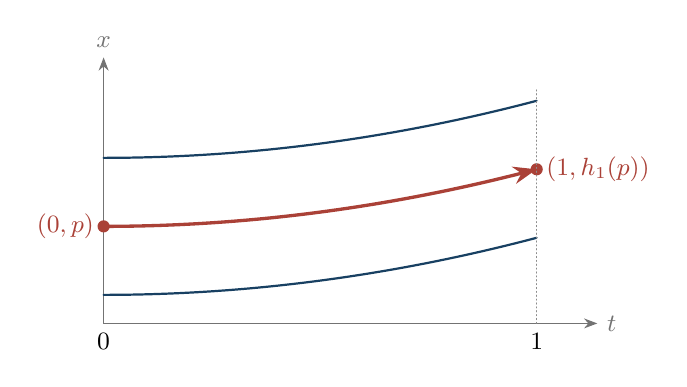
\begin{tikzpicture}[>=Stealth,x=5.5cm,y=1.45cm,line cap=round]
  \draw[->,black!55] (0,-.25)--(1.14,-.25)
    node[right,font=\small] {$t$};
  \draw[->,black!55] (0,-.25)--(0,2.08)
    node[above,font=\small] {$x$};
  \foreach \a in {0,1.2}{
    \draw[manifoldblue!70!black,thick]
      plot[domain=0:1,samples=40] (\x,{\a+.5*\x*\x});
  }
  \draw[->,manifoldred,very thick]
    plot[domain=0:1,samples=40] (\x,{.6+.5*\x*\x});
  \fill[manifoldred] (0,.6) circle (2.2pt)
    node[left,font=\small] {$(0,p)$};
  \fill[manifoldred] (1,1.1) circle (2.2pt)
    node[right,font=\small] {$(1,h_1(p))$};
  \draw[black!45,densely dotted] (1,-.25)--(1,1.8);
  \node[below,font=\small] at (0,-.25) {$0$};
  \node[below,font=\small] at (1,-.25) {$1$};
\end{tikzpicture}
\caption{Ślady trzech punktów w czasoprzestrzeni dla
$X_t=t\partial_x$. Przesunięcie od chwili $0$ do $t$
wynosi $t^2/2$; czerwony ślad punktu $p$ ma rosnące
nachylenie, czyli rosnącą prędkość.}
\label{fig:izotopia-zmienna-predkosc}
\end{figure}

Każda izotopia otoczenia jest generowana przez pole zależne od
czasu: dla $q=h_t(p)$ kładziemy
\begin{equation}\label{eq:generator-izotopii}
 (X_t)_q=\left.\frac{\partial h_t(p)}{\partial t}
 \right|_{p=h_t^{-1}(q)}.
\end{equation}
Gładkość tego pola wymaga także gładkości $(t,q)\mapsto h_t^{-1}(q)$.
Wynika ona z twierdzenia o funkcji odwrotnej zastosowanego do
$H(t,p)=(t,h_t(p))$: różniczka jest blokowo trójkątna z
odwracalnymi blokami $1$ i $\dd h_t$. Przy $t=0,1$ stosujemy
lokalne przedłużenia; pierwsza współrzędna pozostaje czasem.
Jednoznaczność rozwiązań daje $h_t=F_{t,0}$.
W szczególności pole zależne od czasu
o wspólnym zwartym nośniku buduje izotopię otoczenia
stałą poza tym nośnikiem.

\begin{twierdzenie}[Rozszerzenie izotopii, wersja zwarta]
\label{thm:rozszerzenie-izotopii}
Niech $M$ będzie rozmaitością bez brzegu,
$N$ jej zwartą podrozmaitością bez brzegu,
a $i_t\colon N\hookrightarrow M$, $t\in[0,1]$, gładką
izotopią zanurzeń. Istnieje izotopia otoczenia $h_t$ taka, że
$h_t\circ i_0=i_t$. Jej nośnik można umieścić w dowolnym
otwartym otoczeniu zwartego śladu
$\bigcup_{t\in[0,1]}i_t(N)$.
\end{twierdzenie}
Jest to zwarta wersja twierdzenia o rozszerzaniu izotopii;
por.\ \href{https://webhomes.maths.ed.ac.uk/~v1ranick/papers/hirschdx.pdf}
{M. Hirsch, \emph{Differential Topology}, rozdział~8, \S\,1,
Twierdzenie~1.3}.
\begin{proof}
\emph{Krok 1: pole na śladzie izotopii.}
Zbudujmy \emph{ślad w czasoprzestrzeni}
\[
 \mathcal T:=\{(t,i_t(x)):t\in[0,1],\ x\in N\}
 \subset[0,1]\times M.
\]
Odwzorowanie $I(t,x)=(t,i_t(x))$ jest różnowartościowe:
z równości pierwszych współrzędnych mamy ten sam $t$,
a różnowartościowość $i_t$ daje ten sam $x$.
Jego różniczka jest injektywna: jeśli
$\dd I_{(t,x)}(a,v)=0$, to pierwsza współrzędna daje
$a=0$, a następnie $\dd (i_t)_x(v)=0$ wymusza $v=0$.
Ponieważ $[0,1]\times N$ jest zwarta, $I$ jest zanurzeniem
(ciągła bijekcja z przestrzeni zwartej na podprzestrzeń
Hausdorffa ma ciągłą odwrotność). Zatem $\mathcal T$
jest zwartą podrozmaitością z brzegiem w $[0,1]\times M$.
Wyjaśnijmy postać lokalną także dla $t=0,1$. W lokalnych
współrzędnych $u$ na $N$ wybieramy $k=\dim N$ składowych $i_t(u)$,
których różniczka względem $u$ jest odwracalna. Odwzorowanie
$(t,u)\mapsto(t,i_t^1(u),\ldots,i_t^k(u))$ jest lokalnym
dyfeomorfizmem. Pozostałe składowe śladu są więc wykresem
$w=b(t,z)$. Zmiana $(t,z,w)\mapsto(t,z,w-b(t,z))$ prostuje
ślad i zachowuje czas, a zatem również brzeg przy $t=0,1$.
Homeomorficzność $I$ na obraz pozwala zmniejszyć otoczenie tak,
aby nie zawierało innych fragmentów śladu.
Wzdłuż niej mamy dobrze określony \emph{pionowy} wektor
\[
 V(t,i_t(x)):=\frac{\partial i_t(x)}{\partial t}
 \in T_{i_t(x)}M.
\]
Jest gładki, bo $I$ ma gładką odwrotność na $\mathcal T$.

\emph{Krok 2: przedłużenie o małym nośniku.}
Niech $O\subset M$ będzie wskazanym otwartym otoczeniem
rzutu $\mathcal T$ na $M$. Wokół każdego punktu
$\mathcal T$ wybieramy lokalne współrzędne na
$[0,1]\times M$, w których $\mathcal T$ ma postać
normalną opisaną powyżej; otoczenia wybieramy wewnątrz
$[0,1]\times O$. W lokalnej trywializacji $TM$
składowe wektora $V$ są gładkimi funkcjami współrzędnych
na $\mathcal T$; przedłużamy je, nadając im te same
wartości w pobliskich kierunkach normalnych.
Otrzymujemy lokalne pola pionowe $V^{(j)}$, których
ograniczenia do $\mathcal T$ są równe $V$.
Zwartość $\mathcal T$ pozwala wybrać skończenie wiele
takich otoczeń i nieujemne gładkie funkcje odcinające $\chi_j$
o zwartych nośnikach w tych otoczeniach, z
$\sum_j\chi_j>0$ na $\mathcal T$.
Na otwartym zbiorze $U=\{\sum_j\chi_j>0\}$ kładziemy
$Y=(\sum_j\chi_j V^{(j)})/(\sum_k\chi_k)$,
przedłużając każde $\chi_j V^{(j)}$ przez zero poza jego otoczenie.
Na $\mathcal T$ wszystkie składniki $V^{(j)}$ są równe
$V$, więc $Y|_{\mathcal T}=V$.
Wybieramy jeszcze funkcję odcinającą $\rho$ równą $1$ w
otoczeniu zwartej $\mathcal T$, o zwartym nośniku
w $U\subset[0,1]\times O$, i mnożymy przez nią $Y$.
Taka funkcja powstaje ze skończonego pokrycia $\mathcal T$
otoczeniami z funkcjami $0\le\rho_j\le1$, równymi $1$
na mniejszych otoczeniach: $\rho=1-\prod_j(1-\rho_j)$.
Przy końcach czasu wystarczą ograniczenia zwykłych funkcji
odcinających do półprzestrzeni. Warunek $\supp\rho\subset U$
zapewnia, że nie dzielimy przez zero.
Przedłużenie przez zero definiuje gładkie pole $X_t$
na całym $M$, gładkie w $t$, którego wszystkie nośniki
leżą w jednym zwartym $K\subset O$ (rzucie $\supp\rho$ na $M$)
i które spełnia
$(X_t)_{i_t(x)}=\partial_t i_t(x)$.

\emph{Krok 3: całkowanie.} Każda krzywa
$t\mapsto i_t(x)$ spełnia równanie
$\dot q(t)=(X_t)_{q(t)}$ z warunkiem początkowym
$q(0)=i_0(x)$. Lokalna jednoznaczność dla pola zależnego
od czasu wynika z tego samego argumentu co
Twierdzenie~\ref{thm:ode}, po dodaniu czasu jako zmiennej.
Wspólny zwarty nośnik $K$ wyklucza ucieczkę rozwiązania
w skończonym czasie, więc ewolucja $F_{t,s}$ istnieje
dla $s,t\in[0,1]$. Z jednoznaczności
$F_{t,0}(i_0(x))=i_t(x)$. Kładąc $h_t:=F_{t,0}$,
otrzymujemy izotopię dyfeomorfizmów:
jej odwrotnością w chwili $t$ jest $F_{0,t}$.
Poza $K$ pole $X_t$ znika, zatem punkty tam pozostają
nieruchome i nośnik $h_t$ leży w $O$.
\end{proof}

\begin{przyklad}[Przesuwanie punktu]
Gdy $i_t\colon\{*\}\hookrightarrow M$ opisuje gładką drogę
$p_t$ w spójnej składowej $M$, rozszerzenie izotopii daje
rodzinę dyfeomorfizmów $h_t$ z $h_t(p_0)=p_t$.
Można ją zbudować konkretnie, przedłużając prędkość
$\dot p_t$ do pola wspieranego w małym otoczeniu całej drogi.
To narzędzie pozwala przesuwać lokalne konstrukcje
bez zmieniania odległych części rozmaitości.
\end{przyklad}

\begin{uwaga}[Kołnierz brzegu]
Jeśli $M$ ma zwarty brzeg, wybieramy pole $X$, które na
$\partial M$ jest skierowane do wnętrza i poprzeczne do brzegu.
Jego mały dodatni przepływ daje dyfeomorfizm na obraz
$\partial M\times[0,\varepsilon)\to M$,
$(p,t)\mapsto\Phi_t(p)$, zwany \emph{kołnierzem}.
Pole takie otrzymujemy z lokalnych pól skierowanych do wnętrza
przez nieujemne funkcje odcinające; dodatnia składowa normalna
pozostaje dodatnia przy ich sumowaniu. W mapach półprzestrzeni
przedłużamy pole za brzeg, aby zastosować lokalne twierdzenie
o przepływie. Jego dodatnie trajektorie pozostają początkowo w $M$.
Różniczka $(v,a)\mapsto v+aX_p$ jest izomorfizmem w $(p,0)$.
Twierdzenie o funkcji odwrotnej, z uwzględnieniem znaku składowej
normalnej, daje lokalny dyfeomorfizm półotoczeń. Zwartość brzegu
pozwala wybrać wspólny czas istnienia i lokalnej odwracalności.
Pozostaje globalna injektywność dla małego czasu. Gdyby żadna
wartość $\varepsilon$ jej nie dawała, istniałyby różne pary
$(p_j,t_j),(q_j,s_j)$ o tym samym obrazie i $0\le t_j,s_j<1/j$.
Po przejściu do podciągu $p_j\to p$, $q_j\to q$; ciągłość
daje $p=q$. Obie pary leżą wtedy w jednym otoczeniu lokalnej
injektywności przy $(p,0)$, sprzeczność. Obraz jest otwartym
otoczeniem brzegu w $M$, bo mapa jest lokalnym dyfeomorfizmem
półotoczeń. Kołnierz pozwala opisywać otoczenie brzegu
wspólną współrzędną normalną $t$ oraz lokalnymi współrzędnymi
na $\partial M$.
\end{uwaga}

\par\smallskip
{\footnotesize\noindent\emph{Dalsza lektura:}
\href{https://doi.org/10.1007/978-1-4419-9982-5}
{J. M. Lee, \emph{Introduction to Smooth Manifolds}, wyd. 2},
rozdziały 8--9: pola, przepływy (także przy brzegu),
pochodna Liego i pola zależne od czasu;
rozdział 12: rozszerzenie pochodnej Liego na pola tensorowe;
\href{https://people.dm.unipi.it/benedett/MILNOR-TDVPOINT.pdf}
{J. Milnor, \emph{Topology from the Differentiable Viewpoint}},
§4, s.~20--24: gładka izotopia i przemieszczanie punktów
przez przepływ; §6, s.~32--41: pola wektorowe i liczba Eulera.\par}
\clearpage

\chapter{Algebra tensorowa i zewnętrzna}
\label{ch:algebra-tensorowa}

\providecommand{\atlasref}[2]{#2}

\index{tensor}

Wektor styczny i kowektor z Rozdziału~\ref{ch:rozmaitosci} są obiektami
liniowymi. Do opisu odwzorowań wieloliniowych, operatorów i
wyznaczników potrzebujemy przestrzeni, w której symbole
$v\otimes w$ spełniają dokładnie relacje wymuszone przez dwuliniowość.
Zbudujemy ją bez wyboru bazy, a dopiero potem wyprowadzimy rachunek
współrzędnych. W całym rozdziale $\mathbb K=\R$ albo $\C$;
przestrzenie mają skończony wymiar, chyba że zaznaczono inaczej.
W przypadku zespolonym wszystkie odwzorowania wieloliniowe są
$\C$-liniowe w każdym argumencie: nie stosujemy tu sprzężenia
zespolonego. W szczególności dualność algebraiczna nie jest
utożsamieniem przez iloczyn hermitowski.

\section{Iloczyn tensorowy: definicja, istnienie i jednoznaczność}
\label{sec:iloczyn-tensorowy}

\noindent\emph{Powiązania tematyczne w Bibliotece matematycznej:} \atlasref{LA-10::thm:lin10-istnienie}{LA-10: konstrukcja iloczynu tensorowego}.


\begin{definicja}[Własność uniwersalna]
\index{wlasnosc uniwersalna@Własność uniwersalna}
\label{def:tensor-universal}
\emph{Iloczynem tensorowym} przestrzeni $V,W$ nazywamy parę
$(T,\tau)$, gdzie $T$ jest przestrzenią liniową,
$\tau\colon V\times W\to T$ jest odwzorowaniem dwuliniowym,
a dla każdej przestrzeni $Z$ i każdego odwzorowania dwuliniowego
$B\colon V\times W\to Z$ istnieje dokładnie jedno odwzorowanie
liniowe $\widetilde B\colon T\to Z$ takie, że
$B=\widetilde B\circ\tau$. Piszemy $T=V\otimes W$ i
$\tau(v,w)=v\otimes w$. Elementy $v\otimes w$ nazywamy
\emph{tensorami prostymi}.
\end{definicja}

Rysunek~\ref{fig:tensor-wlasnosc-uniwersalna} pokazuje sens definicji:
parę argumentów zastępujemy tensorem $v\otimes w$, a wartość
każdej reguły dwuliniowej obliczamy przez odpowiednie
odwzorowanie liniowe $\widetilde B$.
\begin{figure}[H]
\centering
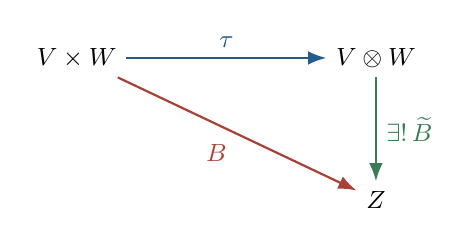
\begin{tikzpicture}[>=Latex, every node/.style={font=\small}]
 \node (vw) at (0,1.8) {$V\times W$};
 \node (tensor) at (3.8,1.8) {$V\otimes W$};
 \node (z) at (3.8,0) {$Z$};
 \draw[->,thick,manifoldblue] (vw) -- node[above] {$\tau$} (tensor);
 \draw[->,thick,manifoldred] (vw) -- node[below left] {$B$} (z);
 \draw[->,thick,manifoldgreen] (tensor) -- node[right] {$\exists!\,\widetilde B$} (z);
\end{tikzpicture}
\caption{Własność uniwersalna: trójkąt komutuje, czyli
$B(v,w)=\widetilde B(v\otimes w)$ dla każdej pary $(v,w)$.}
\label{fig:tensor-wlasnosc-uniwersalna}
\end{figure}

Samo zapisanie $v\otimes w$ nie jest definicją: najpierw trzeba
wykazać, że przestrzeń o tej własności istnieje.

\begin{uwaga}[Co znaczy ,,formalna kombinacja liniowa''?]
\label{rem:kombinacje-formalne}
Jeśli $S$ jest dowolnym zbiorem, \emph{wolna przestrzeń liniowa}
o bazie symboli $[s]$, $s\in S$, składa się z zapisów
\[
 \sum_{s\in S} c_s[s],\qquad c_s\in\mathbb K,
 \quad c_s=0\text{ poza skończoną liczbą indeksów}.
\]
To jest kombinacja \emph{formalna}: dodajemy współczynniki
stojące przy tym samym symbolu i mnożymy je przez skalary,
ale nie przypisujemy symbolom żadnych innych relacji.
Dwa takie zapisy są równe dokładnie wtedy, gdy ich
współczynniki przy każdym $[s]$ są równe. W szczególności
$[s]$ i $[s']$ są niezależnymi wektorami, jeśli $s\ne s'$.
Można myśleć o takim zapisie jako o funkcji
$s\mapsto c_s$ o \emph{skończonym nośniku}.

W dowodzie poniżej bierzemy $S=V\times W$. Jeśli
$v,v'$ są niezależne, symbole $[(v+v',w)]$, $[(v,w)]$
i $[(v',w)]$ mają różne indeksy, więc przed podzieleniem
przez relacje są niezależne. Dopiero iloraz nakazuje równość
$[(v+v',w)]+R=[(v,w)]+[(v',w)]+R$.
Równość dwóch klas $x+R=y+R$ oznacza dokładnie $x-y\in R$.
Ta ostatnia reguła wyjaśnia, dlaczego relacje dwuliniowości
pojawiają się w konstruowanej przestrzeni, a nie były
ukrytym założeniem o symbolach.
\end{uwaga}

\begin{twierdzenie}[Konstrukcja iloczynu tensorowego]
\label{thm:tensor-istnienie}
Dla dowolnych przestrzeni liniowych $V,W$ iloczyn tensorowy istnieje.
Ponadto tensory proste rozpinają $V\otimes W$.
\end{twierdzenie}
\begin{proof}
Niech $F$ będzie wolną przestrzenią liniową o bazie formalnych
symboli $[(v,w)]$, po jednym dla każdej pary $(v,w)\in V\times W$.
Jej elementy są kombinacjami z Uwagi~\ref{rem:kombinacje-formalne}.
Ta pomocnicza przestrzeń jest na ogół nieskończenie wymiarowa,
nawet gdy $V,W$ mają skończony wymiar; dopiero iloraz narzuci relacje.
Niech $R\subseteq F$ będzie podprzestrzenią rozpiętą przez
wszystkie elementy czterech rodzajów:
\begin{align*}
 &[(v+v',w)]-[(v,w)]-[(v',w)],
 &&[(av,w)]-a[(v,w)],\\
 &[(v,w+w')]-[(v,w)]-[(v,w')],
 &&[(v,aw)]-a[(v,w)],
\end{align*}
gdzie $a\in\mathbb K$. Kładziemy $T:=F/R$ oraz
$v\otimes w:=[(v,w)]+R$. Cztery relacje pokazują kolejno,
że $\tau(v,w):=v\otimes w$ jest liniowa w każdej zmiennej.
Każda klasa w $F/R$ jest skończoną kombinacją liniową klas $[(v,w)]+R$,
więc tensory proste rozpinają $T$.

Weźmy teraz dowolne odwzorowanie dwuliniowe $B\colon V\times W\to Z$.
Na $F$ istnieje dokładnie jedno odwzorowanie liniowe
$L\colon F\to Z$ o wartościach $L([(v,w)])=B(v,w)$:
określamy je na bazie i przedłużamy liniowo. Dwuliniowość $B$
oznacza, że $L$ zeruje każdy z czterech typów generatorów $R$,
a więc $R\subseteq\ker L$. Odwzorowanie $L$ przechodzi na iloraz:
$\widetilde B(x+R):=L(x)$ dla $x\in F$. Jest dobrze określone, bo
$x+R=x'+R$ implikuje $L(x-x')=0$, i spełnia
$\widetilde B(v\otimes w)=B(v,w)$. Jeśli drugie odwzorowanie liniowe
spełniałoby tę samą równość, zgadzałoby się z $\widetilde B$
na zbiorze rozpinającym $T$, a zatem wszędzie.
\end{proof}

W praktyce faktoryzacja działa na dowolnej skończonej sumie:
\[
 \widetilde B\!\left(\sum_{a=1}^N c_a v_a\otimes w_a\right)
   =\sum_{a=1}^N c_a B(v_a,w_a).
\]
Ten wzór nie zależy od wybranego zapisu tensora jako sumy:
wynika z odwzorowania $L$, które zeruje wszystkie relacje tworzące $R$.
Relacje nie zerują też niezerowego tensora prostego. Jeżeli
$v\ne0$ i $w\ne0$, dopełniamy je do baz i wybieramy
$\alpha\in V^*$, $\beta\in W^*$ z
$\alpha(v)=\beta(w)=1$. Dla dwuliniowego
$B(x,y)=\alpha(x)\beta(y)$ mamy
$\widetilde B(v\otimes w)=1$, więc $v\otimes w\ne0$.

\begin{uwaga}[Faktoryzacja przez iloraz a izomorfizm]
\label{rem:tensor-iloraz-izomorfizm}
W dowodzie wystarczyło $R\subseteq\ker L$, aby otrzymać
odwzorowanie $\widetilde B:F/R\to Z$. To jest ten sam mechanizm
przechodzenia do ilorazu, który w ogólnej postaci
porządkuje Twierdzenie~\ref{thm:modul-izomorfizm}
w Rozdziale~\ref{ch:algebra-abstrakcyjna}
(przestrzenie liniowe są modułami nad $\mathbb K$).
Pełne twierdzenie daje $F/\ker L\cong\operatorname{im}L$.
Nie utożsamiamy natomiast $F/R$ z $\operatorname{im}L$,
chyba że $R=\ker L$; do istnienia iloczynu tensorowego
taka równość nie jest potrzebna.
\end{uwaga}

\begin{twierdzenie}[Jednoznaczność]
\label{thm:tensor-jednoznacznosc}
Jeżeli $(T,\tau)$ i $(T',\tau')$ spełniają
Definicję~\ref{def:tensor-universal}, istnieje dokładnie jeden
izomorfizm spełniający
\[
 J\colon T\to T',\qquad J\circ\tau=\tau'.
\]
\end{twierdzenie}
\begin{proof}
Własność uniwersalna $(T,\tau)$ zastosowana do $\tau'$ daje
jedyne odwzorowanie liniowe $J\colon T\to T'$ z~żądaną własnością.
Podobnie $(T',\tau')$ daje $K\colon T'\to T$ z
$K\circ\tau'=\tau$. Zatem $(K\circ J)\circ\tau=\tau$.
Również $\id_T\circ\tau=\tau$; jednoznaczność faktoryzacji
przez $T$ wymusza $K\circ J=\id_T$. Tak samo $J\circ K=\id_{T'}$.
Odwzorowanie $J$ jest więc izomorfizmem i jedynym możliwym odwzorowaniem
zachowującym wskazane obrazy par $(v,w)$.
\end{proof}

\begin{przyklad}[Wyznacznik jako odwzorowanie liniowe na tensorach]
Niech $V=W=\R^2$ i
$B(v,w)=v_1w_2-v_2w_1=\det(v,w)$.
Dwuliniowość wyznacznika daje dokładnie jedno
$\widetilde B\colon\R^2\otimes\R^2\to\R$ takie, że
\[
 \widetilde B\!\left(\sum_{a=1}^N c_a v_a\otimes w_a\right)
 =\sum_{a=1}^N c_a\det(v_a,w_a).
\]
Na wektorach bazy standardowej
$\widetilde B(e_1\otimes e_2)=1$ i
$\widetilde B(e_2\otimes e_1)=-1$.
Zatem $e_1\otimes e_2\ne e_2\otimes e_1$:
w zwykłym iloczynie tensorowym przestawienie czynników
nie jest równością tensorów. Na przykład
$\widetilde B(2e_1\otimes e_2-e_2\otimes e_1)=3$.
\end{przyklad}

W szczególności
\begin{equation}\label{eq:tensor-biliniowosc}
 (av+bv')\otimes w=a(v\otimes w)+b(v'\otimes w),\qquad
 v\otimes(aw+bw')=a(v\otimes w)+b(v\otimes w').
\end{equation}
\emph{Każdy} element $V\otimes W$ jest skończoną sumą tensorów
prostych, ale nie musi sam być tensorem prostym.

\section{Baza, wymiar i wiele czynników}
\label{sec:baza-tensorowa}

Wybór baz pozwala zapisać tensor jako tablicę współczynników.
Najpierw sprawdzimy, że każdy element ma dokładnie jedną taką tablicę;
liczba jej pól wyjaśni wymiar iloczynu tensorowego.

\begin{twierdzenie}[Baza iloczynu tensorowego]
\label{thm:baza-tensorowa}
Jeżeli $e_1,\ldots,e_m$ jest bazą $V$, a
$f_1,\ldots,f_n$ bazą $W$, to
\[
 \bigl\{e_i\otimes f_j:1\leq i\leq m,\;1\leq j\leq n\bigr\}
\]
jest bazą $V\otimes W$. W szczególności
$\dim(V\otimes W)=mn$.
\end{twierdzenie}
\begin{proof}
Dla $v=\sum_i a_i e_i$ i $w=\sum_j b_j f_j$ dwuliniowość daje
\[
 v\otimes w=\sum_{i=1}^m\sum_{j=1}^n a_ib_j(e_i\otimes f_j).
\]
Ponieważ tensory proste rozpinają $V\otimes W$, wyświetlone
wektory są układem rozpinającym. Dla liniowej niezależności
wprowadźmy przestrzeń $\mathbb K^{m\times n}$ z bazą jednostek
macierzowych $E_{ij}$: jedynka na miejscu $(i,j)$ i zera poza nim. Przypisanie
$B(v,w)=(a_i b_j)_{i,j}$ jest dwuliniowe; własność uniwersalna
daje $\widetilde B\colon V\otimes W\to\mathbb K^{m\times n}$
z $\widetilde B(e_i\otimes f_j)=E_{ij}$. Jeśli
$\sum_{i,j}c_{ij}e_i\otimes f_j=0$, zastosowanie
$\widetilde B$ daje $\sum_{i,j}c_{ij}E_{ij}=0$, czyli
wszystkie $c_{ij}=0$. Każdy tensor ma więc jednoznaczną postać
$T=\sum_{i,j}c_{ij}e_i\otimes f_j$, a $\widetilde B(T)=(c_{ij})$.
Tak wykazaliśmy również podany wymiar.
\end{proof}

Utożsamienie $T$ z macierzą $(c_{ij})$ zależy od wybranych baz.
Sam tensor i jego własność prostoty od nich nie zależą.

\begin{przyklad}[Tensor prosty a suma tensorów]
Dla $V=W=\R^2$ odwzorowanie z dowodu przypisuje
$(1,2)\otimes(3,-1)$ macierz
$\begin{psmallmatrix}3&-1\\6&-2\end{psmallmatrix}$.
Każdy niezerowy tensor prosty ma tu macierz rzędu $1$:
jest ona iloczynem kolumny współrzędnych $v$ i wiersza
współrzędnych $w$. Odwrotnie, każda macierz rzędu $1$
ma postać $ab^{\mathsf T}$: wybieramy niezerową kolumnę $a$,
a pozostałe kolumny są jej wielokrotnościami $b_j a$.
Macierz zerowa odpowiada tensorowi prostemu $0\otimes w=0$.
Zatem na $\R^2\otimes\R^2$ tensor jest prosty dokładnie wtedy,
gdy jego macierz ma rząd co najwyżej $1$, czyli wyznacznik $0$.
Natomiast
$e_1\otimes e_1+e_2\otimes e_2$ odpowiada macierzy
identycznościowej rzędu $2$, więc nie jest prosty.
Należy też pamiętać, że $v\otimes w$ nie oznacza pary $(v,w)$:
na przykład $(2v)\otimes w=v\otimes(2w)$.
\end{przyklad}

\begin{figure}[H]
\centering
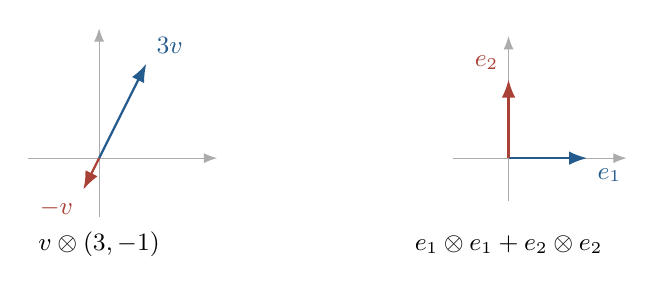
\begin{tikzpicture}[>=Latex, every node/.style={font=\small}]
 \begin{scope}[xshift=-2.6cm]
  \draw[gray!65,->] (-0.9,0)--(1.5,0);
  \draw[gray!65,->] (0,-0.75)--(0,1.65);
  \draw[manifoldblue,thick,->] (0,0)--(0.6,1.2)
    node[above right] {$3v$};
  \draw[manifoldred,thick,->] (0,0)--(-0.2,-0.4)
    node[below left] {$-v$};
  \node at (0,-1.1) {$v\otimes(3,-1)$};
 \end{scope}
 \begin{scope}[xshift=2.6cm]
  \draw[gray!65,->] (-0.7,0)--(1.5,0);
  \draw[gray!65,->] (0,-0.55)--(0,1.55);
  \draw[manifoldblue,thick,->] (0,0)--(1,0)
    node[below right] {$e_1$};
  \draw[manifoldred,thick,->] (0,0)--(0,1)
    node[above left] {$e_2$};
  \node at (0,-1.1) {$e_1\otimes e_1+e_2\otimes e_2$};
 \end{scope}
\end{tikzpicture}
\caption{Kolumny macierzy tensora prostego są współliniowe (po lewej:
$v=(1,2)$, kolumny $3v$ i $-v$). Dwie kolumny macierzy
identycznościowej są niezależne, więc odpowiadający jej tensor nie jest prosty.}
\label{fig:tensor-prosty-rzad}
\end{figure}

\begin{stwierdzenie}[Łączność i przestawianie czynników]
\label{prop:tensor-lacznosc}
Istnieją kanoniczne izomorfizmy
\[
 (V\otimes W)\otimes U\longrightarrow V\otimes(W\otimes U),
 \quad (v\otimes w)\otimes u\longmapsto v\otimes(w\otimes u),
\]
\[
 V\otimes W\longrightarrow W\otimes V,
 \quad v\otimes w\longmapsto w\otimes v.
\]
Dlatego możemy pisać $V_1\otimes\cdots\otimes V_k$ bez nawiasów.
\end{stwierdzenie}
\begin{proof}
Odwzorowanie $(v,w,u)\mapsto v\otimes(w\otimes u)$ jest
trójliniowe. Każde odwzorowanie trójliniowe na $V\times W\times U$
faktoryzuje jednoznacznie przez $(V\otimes W)\otimes U$:
gdy $H\colon V\times W\times U\to Z$ jest trójliniowe,
przy ustalonym $u$ kładziemy $H_u(v,w):=H(v,w,u)$
i faktoryzujemy je do liniowego $L_u\colon V\otimes W\to Z$.
Równość
$L_{au+bu'}(v\otimes w)=aL_u(v\otimes w)+bL_{u'}(v\otimes w)$
na tensorach prostych daje $L_{au+bu'}=aL_u+bL_{u'}$.
Stąd $(t,u)\mapsto L_u(t)$ jest dwuliniowe i faktoryzuje
przez $(V\otimes W)\otimes U$. Otrzymujemy zatem odwzorowanie w treści
stwierdzenia. Analogiczna konstrukcja w drugą stronę daje
$v\otimes(w\otimes u)\mapsto(v\otimes w)\otimes u$.
Oba złożenia są identycznością na tensorach prostych trzech
czynników, które rozpinają odpowiednie przestrzenie.
Izomorfizm przestawiający dwa czynniki pochodzi z dwuliniowego
odwzorowania $(v,w)\mapsto w\otimes v$; jego odwrotność powstaje
po ponownym przestawieniu.
Na współczynnikach $v\otimes w=\sum_{i,j}a_i b_j e_i\otimes f_j$
przestawienie odpowiada transpozycji tablicy $(a_i b_j)$;
przez liniowość ten sam opis działa dla dowolnego tensora.
Jest to kanoniczny izomorfizm przestrzeni tensorowych,
nie dosłowna równość ich elementów.
Przy większej liczbie czynników dowolne dwa sposoby zmiany
nawiasowania dają to samo odwzorowanie: na każdym tensorze
prostym zachowują kolejność i wartości wszystkich czynników,
a takie tensory rozpinają dziedzinę. To uzasadnia pomijanie
nawiasów również dla czterech i więcej przestrzeni.
\end{proof}

Kładziemy $V^{\otimes0}:=\mathbb K$ oraz
$V^{\otimes k}:=V\otimes\cdots\otimes V$ dla $k\geq1$.
Uzasadnia to kanoniczny izomorfizm
$\mathbb K\otimes U\cong U$, $a\otimes u\mapsto au$,
z odwrotnością $u\mapsto1\otimes u$; analogicznie
$U\otimes\mathbb K\cong U$. Będziemy stosować te
utożsamienia także wtedy, gdy $U=\mathbb K$.
Jeżeli $\dim V=n$, iterowanie Twierdzenia~\ref{thm:baza-tensorowa}
daje bazę $e_{i_1}\otimes\cdots\otimes e_{i_k}$ i wymiar
\begin{equation}\label{eq:dim-potega-tensorowa}
 \dim V^{\otimes k}=n^k\qquad(k\geq0).
\end{equation}
Dla $k=0$ bazą jest $\{1\}$ i przyjmujemy $n^0=1$,
również gdy $V=0$. Na przykład
$\dim(\R^2)^{\otimes3}=2^3=8$.

\section{Tensory mieszane i operacje na nich}
\label{sec:operacje-tensorowe}

Oznaczmy $V^*:=\operatorname{Hom}_{\mathbb K}(V,\mathbb K)$.
Jest to przestrzeń liniowych funkcjonałów, zwanych kowektorami.
Dla nieujemnych $r,s$ przyjmujemy konwencję
\begin{equation}\label{eq:typ-tensora}
 T^r_s(V):=V^{\otimes r}\otimes(V^*)^{\otimes s}.
\end{equation}
Tensory typu $(r,s)$ mają $r$ czynników wektorowych i $s$
kowektorowych; powiązane z nimi funkcje wieloliniowe
przyjmują $r$ kowektorów i $s$ wektorów. Na tensorze prostym
dla $r+s>0$ wyznacza je wzór
\[
 (v_1\otimes\cdots\otimes v_r\otimes
 \alpha_1\otimes\cdots\otimes\alpha_s)
 (\xi_1,\ldots,\xi_r;w_1,\ldots,w_s)
 =\prod_{a=1}^r\xi_a(v_a)\prod_{b=1}^s\alpha_b(w_b).
\]
Puste iloczyny mają wartość $1$. Dla $r=s=0$ mamy
$T^0_0(V)=\mathbb K$ po kanonicznym utożsamieniu
$\mathbb K\otimes\mathbb K\cong\mathbb K$ z poprzedniej sekcji.
Skalar $c$ przyjmuje na jedynym pustym układzie argumentów
wartość $c$; dziedziną takiej funkcji jest zbiór jednoelementowy.

\begin{twierdzenie}[Postać wieloliniowa tensora]
\label{thm:tensor-wieloliniowy}
Dla skończenie wymiarowej przestrzeni $V$ powyższy wzór daje
izomorfizm
\[
 T^r_s(V)\cong
 \operatorname{Mult}\bigl((V^*)^r\times V^s,\mathbb K\bigr).
\]
Jeśli $e_1,\ldots,e_n$ jest bazą $V$ i $e^1,\ldots,e^n$
bazą dualną, każdy tensor ma dokładnie jedno rozwinięcie
\begin{equation}\label{eq:wspolczynniki-tensora}
 T=\sum_{\substack{i_1,\ldots,i_r\\j_1,\ldots,j_s}}
 T^{i_1\cdots i_r}{}_{j_1\cdots j_s}
 e_{i_1}\otimes\cdots\otimes e_{i_r}
 \otimes e^{j_1}\otimes\cdots\otimes e^{j_s}.
\end{equation}
\end{twierdzenie}
\begin{proof}
Rozwinięcie i jego jednoznaczność wynikają z kolejnych
zastosowań Twierdzenia~\ref{thm:baza-tensorowa}. Wzór
na działanie na argumentach jest wieloliniowy w czynnikach
tensora, więc przez własność uniwersalną definiuje odwzorowanie liniowe
$T^r_s(V)$ do wskazanej przestrzeni funkcji. Aby wykazać jego
iniektywność, podstawmy w miejsce argumentów elementy baz:
\[
 e^{i_1},\ldots,e^{i_r};\qquad e_{j_1},\ldots,e_{j_s}.
\]
Uzyskana wartość jest dokładnie współczynnikiem
$T^{i_1\cdots i_r}{}_{j_1\cdots j_s}$. Jeśli wszystkie wartości
są zerowe, znikają więc wszystkie współczynniki.
Odwrotnie, dla dowolnej funkcji wieloliniowej $F$ wstawmy te
wartości do prawej strony~\eqref{eq:wspolczynniki-tensora}.
Otrzymany tensor ma te same wartości co $F$ na wszystkich
układach elementów bazowych. Rozwinięcie argumentów i ich
wieloliniowość dają równość na dowolnych argumentach.
\end{proof}

Współczynniki tensora są jego wartościami na wskazanych układach
wektorów i kowektorów bazowych. Zmieniają się po zmianie bazy,
choć sam tensor i określona przez niego funkcja pozostają te same.

Przykładowo $T^0_2(V)$ to formy dwuliniowe na $V$.
Związek tensorów z operatorami wymaga pilnowania,
z której przestrzeni operator \emph{przyjmuje} argument.

\begin{twierdzenie}[Tensory i przestrzenie operatorów]
\label{thm:tensor-hom}
Dla skończenie wymiarowych $V,W$ istnieje kanoniczny izomorfizm
\begin{equation}\label{eq:tensor-hom}
 \Theta_{V,W}\colon V\otimes W^*\longrightarrow
 \operatorname{Hom}_{\mathbb K}(W,V),\qquad
 \Theta_{V,W}(v\otimes\lambda)(w):=\lambda(w)v.
\end{equation}
W szczególności po zamianie nazw przestrzeni otrzymujemy
$W\otimes V^*\cong\operatorname{Hom}_{\mathbb K}(V,W)$.
\end{twierdzenie}
\begin{proof}
Dla ustalonego $w\in W$ wyrażenie $\lambda(w)v$ zależy
liniowo od $v$ oraz liniowo od $\lambda$; samo przypisanie
$w\mapsto\lambda(w)v$ jest liniowe. Dlatego odwzorowanie
$(v,\lambda)\mapsto(w\mapsto\lambda(w)v)$ ma wartości
w $\operatorname{Hom}(W,V)$ i jest dwuliniowe.
Własność uniwersalna iloczynu tensorowego wyznacza
\emph{jedno} odwzorowanie liniowe $\Theta_{V,W}$ o wzorze
\eqref{eq:tensor-hom}. Tym samym wzór działa również
na sumach: $\Theta_{V,W}(\sum_a v_a\otimes\lambda_a)(w)
=\sum_a\lambda_a(w)v_a$. Nie musimy wybierać sposobu
zapisania takiej sumy, bo $\Theta_{V,W}$ została zdefiniowana
na całej przestrzeni tensorowej.

Zbudujmy odwrotność. Wybierzmy bazę $f_1,\ldots,f_m$
przestrzeni $W$ i jej bazę dualną $f^1,\ldots,f^m$.
Dla $A\in\operatorname{Hom}(W,V)$ połóżmy
\begin{equation}\label{eq:hom-tensor-odwrotna}
 \mathcal I(A):=\sum_{j=1}^m A(f_j)\otimes f^j\in V\otimes W^*.
\end{equation}
Sprawdzimy oba złożenia. Jeśli $w\in W$, to
\[
 \Theta_{V,W}(\mathcal I(A))(w)
 =\sum_j f^j(w)A(f_j)
 =A\!\left(\sum_j f^j(w)f_j\right)=A(w),
\]
bo $w=\sum_j f^j(w)f_j$. Odwrotnie, dla prostego
tensora $v\otimes\lambda$ mamy
\[
 \mathcal I(\Theta_{V,W}(v\otimes\lambda))
 =\sum_j\lambda(f_j)v\otimes f^j
 =v\otimes\left(\sum_j\lambda(f_j)f^j\right)
 =v\otimes\lambda.
\]
Tensory proste rozpinają $V\otimes W^*$, więc drugie
złożenie też jest identycznością wszędzie. Wzór
\eqref{eq:hom-tensor-odwrotna} wygląda zależnie od bazy,
ale jest odwrotnością kanonicznej $\Theta_{V,W}$;
dlatego jego wynik od bazy nie zależy.
\end{proof}

Tensor prosty $v\otimes\lambda$ działa na $w$ dwuetapowo:
funkcjonał $\lambda$ odczytuje liczbę $\lambda(w)$,
a ta liczba skaluje ustalony wektor $v$.
Obraz operatora mieści się więc w prostej $\mathbb Kv$.
Suma skończonej liczby takich tensorów daje operator skończonej
rangi. Założenie skończonego wymiaru w Twierdzeniu~\ref{thm:tensor-hom}
zapewnia, że każdy operator jest taką sumą;
na przestrzeni nieskończenie wymiarowej identyczność nie ma
skończonej rangi.

Przy $W=V$ otrzymujemy
$T^1_1(V)=V\otimes V^*\cong\operatorname{End}(V)$.
Na tensorze prostym odpowiada temu wzór
\begin{equation}\label{eq:endo-tensor}
 v\otimes\alpha\longmapsto
 \bigl(w\longmapsto\alpha(w)v\bigr).
\end{equation}
Na przykład $e_i\otimes e^j$ przechodzi na jednostkę
macierzową $E_{ij}$: wysyła $e_j$ na $e_i$, a pozostałe
wektory bazowe na zero. W bazie $e'_i=\sum_a A^a{}_i e_a$
macierz operatora $S$ ma postać $[S]'=A^{-1}[S]A$:
zmieniają się współczynniki, nie sam operator.
Istotnie, jeśli $[v]$ i $[v]'$ oznaczają kolumny współrzędnych,
to $[v]=A[v]'$. Stąd $[Sv]'=A^{-1}[S]A[v]'$.
Baza dualna zmienia się według
$e'^i=\sum_b(A^{-1})^i{}_b e^b$, co wynika z warunku
$e'^i(e'_j)=\delta^i_j$; używamy odwrotności bez sprzężenia zespolonego.

\begin{uwaga}[Funkcja dwuliniowa a operator]
\label{rem:mult-hom}
Z Twierdzenia~\ref{thm:tensor-wieloliniowy} dla typu $(1,1)$
dostajemy
\[
 V\otimes V^*\cong\operatorname{Mult}(V^*\times V,\mathbb K).
\]
Dlaczego równie często spotyka się zapis
$\operatorname{Mult}(V\times V^*,\mathbb K)$?
Kolejność argumentów można po prostu zamienić: jeśli
$C(\lambda,v)$ jest dwuliniowa, to $B(v,\lambda):=C(\lambda,v)$
też jest dwuliniowa. Jest to odwracalna operacja, niezależna
od wyboru bazy. W obu zapisach odpowiadający operatorowi
$A\in\operatorname{Hom}(V,V)$ wzór ma postać
\begin{equation}\label{eq:mult-operator}
 B_A(v,\lambda)=\lambda(Av),
 \qquad v\in V,\quad\lambda\in V^*.
\end{equation}
Wektor $v$ jest argumentem operatora $A$; kowektor
$\lambda$ odczytuje liczbę z wyniku $Av$.

Sprawdźmy, że przy $\dim V<\infty$ wzór ten obejmuje
\emph{każdą} taką funkcję dwuliniową $B$. Wybierzmy bazę
$e_1,\ldots,e_n$ i bazę dualną $e^1,\ldots,e^n$, po czym
zdefiniujmy
\[
 A_B(v):=\sum_{i=1}^n B(v,e^i)e_i.
\]
Odwzorowanie $A_B$ jest liniowe, bo $B$ jest liniowa w pierwszym
argumencie. Dla dowolnego $\lambda\in V^*$ zachodzi
\[
 \lambda(A_Bv)=\sum_i B(v,e^i)\lambda(e_i)
 =B\!\left(v,\sum_i\lambda(e_i)e^i\right)=B(v,\lambda).
\]
Jeżeli dwa operatory dają tę samą funkcję $B$, każdy kowektor
przyjmuje na ich wartościach ten sam wynik, więc operatory
są równe. Zatem
$\operatorname{Mult}(V\times V^*,\mathbb K)
 \cong\operatorname{Hom}(V,V)$.
Na przykład tensor $u\otimes\alpha$ odpowiada operatorowi
$A(v)=\alpha(v)u$, a następnie funkcji
$B_A(v,\lambda)=\alpha(v)\lambda(u)$.
Nie utożsamiamy przy tym $V$ z $V^*$; korzystamy jedynie
z naturalnego sparowania $\lambda(v)$.
\end{uwaga}

\begin{przyklad}[Tensor prosty i nieprosty typu $(1,1)$]
Niech $V=\R^2$, niech $e_1,e_2$ będzie jego bazą, a
$e^1,e^2$ bazą dualną. Tensor
\[
 P=(e_1+e_2)\otimes(e^1-e^2)
\]
jest \emph{prosty}: ma postać jednego iloczynu tensorowego.
Odpowiada mu operator $A_P(v)=(e^1(v)-e^2(v))(e_1+e_2)$,
o macierzy
$\begin{psmallmatrix}1&-1\\1&-1\end{psmallmatrix}$.
Wszystkie jego wartości leżą na jednej prostej, więc
$\operatorname{rank}A_P=1$. Jego funkcja dwuliniowa to
$B_P(v,\lambda)=(e^1(v)-e^2(v))\lambda(e_1+e_2)$.

Z kolei tensor
$Q=e_1\otimes e^1+e_2\otimes e^2$ jest
\emph{nieprosty}. Odpowiada mu operator
$A_Q(v)=e^1(v)e_1+e^2(v)e_2=v$, czyli macierz
$\begin{psmallmatrix}1&0\\0&1\end{psmallmatrix}$ i funkcja
$B_Q(v,\lambda)=\lambda(v)$. Gdyby $Q=u\otimes\alpha$,
obraz $A_Q$ mieściłby się w prostej $\mathbb Ku$.
Jednak $A_Q(e_1)=e_1$ i $A_Q(e_2)=e_2$ są niezależne;
stąd $Q$ nie może być jednym tensorem prostym.
\end{przyklad}

\begin{uwaga}[Kolejność czynników jest istotna]
Równość $V\otimes W^*\cong\operatorname{Hom}(V,W)$
nie jest naturalnym utożsamieniem: wzór~\eqref{eq:tensor-hom}
przyjmuje argument $w\in W$ i zwraca wynik w $V$.
Do otrzymania odwzorowań z $V$ do $W$ trzeba wziąć
$W\otimes V^*$. Przestrzenie $V\otimes W^*$ oraz
$\operatorname{Hom}(V,W)$ mają wprawdzie równy wymiar,
ale równość wymiarów daje jedynie istnienie pewnego
izomorfizmu po dokonaniu dodatkowych wyborów, np.\ baz.
\end{uwaga}

\begin{twierdzenie}[Iloczyn tensorowy odwzorowań]
\label{thm:tensor-operatorow}
Dla odwzorowań liniowych $A\colon V\to V'$ i $B\colon W\to W'$
istnieje dokładnie jedno odwzorowanie liniowe
$A\otimes B\colon V\otimes W\to V'\otimes W'$ spełniające
\begin{equation}\label{eq:tensor-operatorow}
 (A\otimes B)(v\otimes w)=Av\otimes Bw.
\end{equation}
Jeżeli $A'\colon V'\to V''$ i $B'\colon W'\to W''$, to
\[
 (A'\otimes B')\circ(A\otimes B)=(A'\circ A)\otimes(B'\circ B),
 \qquad \id_V\otimes\id_W=\id_{V\otimes W}.
\]
Dla przestrzeni skończenie wymiarowych
$\operatorname{rank}(A\otimes B)=\operatorname{rank}A\,\operatorname{rank}B$.
\end{twierdzenie}
\begin{proof}
Odwzorowanie $(v,w)\mapsto Av\otimes Bw$ jest dwuliniowe:
liniowość $A$ i pierwszego miejsca $\otimes$ dają
liniowość w $v$, analogicznie w $w$. Własność uniwersalna
tworzy dokładnie jedno odwzorowanie o wzorze~\eqref{eq:tensor-operatorow}.
Obie strony równości złożeń przyłożone do $v\otimes w$
dają $A'Av\otimes B'Bw$. Tensory proste rozpinają dziedzinę,
więc odwzorowania są równe. Identyczność sprawdzamy tak samo.

Obraz $A\otimes B$ jest rozpięty przez wszystkie $Av\otimes Bw$,
więc równa się $(\operatorname{im}A)\otimes(\operatorname{im}B)$,
rozumianemu jako podprzestrzeń $V'\otimes W'$.
Aby uzasadnić tę ostatnią inkluzję bez ukrytego założenia,
dopełnijmy bazy obu obrazów do baz $V'$ i $W'$;
Twierdzenie~\ref{thm:baza-tensorowa} pokazuje, że iloczyny
wektorów z mniejszych baz pozostają liniowo niezależne
w większym iloczynie tensorowym. Ich liczba to iloczyn rang.
\end{proof}

Jeśli macierze $A,B$ mają współczynniki $a_{pi},b_{qj}$,
to dla baz źródła $e_i,f_j$ i celu $e'_p,f'_q$ mamy
\[
 \begin{aligned}
 (A\otimes B)(e_i\otimes f_j)
 &=\left(\sum_p a_{pi}e'_p\right)\otimes
   \left(\sum_q b_{qj}f'_q\right)\\
 &=\sum_{p,q}a_{pi}b_{qj}\,e'_p\otimes f'_q.
 \end{aligned}
\]
Zatem w bazach tensorowych współczynnik macierzy
$A\otimes B$ o indeksach $(p,q),(i,j)$ jest $a_{pi}b_{qj}$.
Jest to \emph{iloczyn Kroneckera}. Pary porządkujemy
leksykograficznie: $(1,1),(1,2),\ldots,(2,1),\ldots$.
W takim porządku na przykład
\[
 A=\begin{pmatrix}1&2\\0&1\end{pmatrix},\quad
 B=\begin{pmatrix}2&0\\0&3\end{pmatrix},\qquad
 A\otimes B=
 \begin{pmatrix}1B&2B\\0B&1B\end{pmatrix}
 =
 \begin{pmatrix}
 2&0&4&0\\0&3&0&6\\0&0&2&0\\0&0&0&3
 \end{pmatrix}.
\]
Rangę widać także w przykładzie osobliwym: dla
$A=\operatorname{diag}(1,0)$ i $B=\operatorname{diag}(2,3)$
macierz $A\otimes B=\operatorname{diag}(2,3,0,0)$ ma
rangę $2=1\cdot2$.

Iloczyn tensorów mieszanych wymaga ustalenia kolejności.
Jeśli $S\in T^r_s(V)$ i $T\in T^{r'}_{s'}(V)$, ich surowy
iloczyn ma kolejno bloki $V^{\otimes r}$, $(V^*)^{\otimes s}$,
$V^{\otimes r'}$, $(V^*)^{\otimes s'}$. Przenosimy trzeci blok
przed drugi kanonicznym przestawieniem czynników i tak otrzymany
element $T^{r+r'}_{s+s'}(V)$ oznaczamy także $S\otimes T$.
Wewnątrz bloków zachowujemy kolejność. Nie pojawia się znak:
jest to zwykły iloczyn tensorowy, a nie iloczyn zewnętrzny.

\begin{definicja}[Kontrakcja]
\index{kontrakcja@Kontrakcja}
\label{def:kontrakcja}
\emph{Kontrakcja} usuwa jedną parę: czynnik $V$ i czynnik $V^*$,
łącząc je przez ewaluację $\alpha(v)$. W najprostszym przypadku
jest to odwzorowanie $C\colon V\otimes V^*\to\mathbb K$,
$C(v\otimes\alpha)=\alpha(v)$. W~ogólności dostajemy
$C_{a,b}\colon T^r_s(V)\to T^{r-1}_{s-1}(V)$, gdy $r,s\geq1$.
Indeksy spełniają $1\leq a\leq r$ i $1\leq b\leq s$.
Na tensorze prostym mnożymy przez $\alpha_b(v_a)$,
usuwamy czynniki $v_a$ i $\alpha_b$, a pozostałe zachowujemy
w pierwotnej kolejności. Przykładowo kontrakcja pierwszej pary ma współczynniki
\[
 (C_{1,1}T)^{i_2\cdots i_r}{}_{j_2\cdots j_s}
 =\sum_{a=1}^{\dim V}T^{a i_2\cdots i_r}{}_{a j_2\cdots j_s}.
\]
\end{definicja}

Kontrakcja korzysta tylko z naturalnego sparowania
$V^*\times V\to\mathbb K$; nie wymaga iloczynu skalarnego
ani utożsamienia $V$ z $V^*$.

\begin{stwierdzenie}[Kontrakcja i ślad]
\label{prop:kontrakcja-slad}
Kontrakcja jest liniowa i nie zależy od wyboru bazy. Dla
$S=\sum_{i,j}S^i{}_j e_i\otimes e^j\in T^1_1(V)$ zachodzi
\[
 C(S)=\sum_i S^i{}_i=\operatorname{tr}S,
\]
gdzie ostatni ślad dotyczy operatora z~\eqref{eq:endo-tensor}.
\end{stwierdzenie}
\begin{proof}
Ewaluacja $(v,\alpha)\mapsto\alpha(v)$ jest dwuliniowa,
więc ma jednoznaczne przedłużenie do $V\otimes V^*$.
Pozostałe czynniki przestawiamy izomorfizmami ze
Stwierdzenia~\ref{prop:tensor-lacznosc} i stosujemy tę ewaluację
w wybranej parze. Ponieważ definicja używa jedynie wartości
kowektora na wektorze, wynik nie zależy od bazy.
Dla współrzędnych $C(e_i\otimes e^j)=e^j(e_i)=\delta_i^j$,
więc $C(S)=\sum_i S^i{}_i$. Z~\eqref{eq:endo-tensor}
współczynniki $S^i{}_j$ są współczynnikami macierzy operatora,
a powyższa suma jest jej śladem.
Ten sam rachunek wyjaśnia ogólny wzór z
Definicji~\ref{def:kontrakcja}: na tensorze bazowym
ewaluacja pierwszej pary wnosi
$e^{j_1}(e_{i_1})=\delta^{j_1}_{i_1}$.
Przy sumowaniu rozwinięcia \eqref{eq:wspolczynniki-tensora}
zostają więc dokładnie składniki z $i_1=j_1=a$;
sumujemy po $a$, a pozostałe indeksy zachowujemy.
\end{proof}

Rysunek~\ref{fig:kontrakcja-slad} zapisuje tę samą operację
dwiema drogami: bezpośrednią ewaluacją i śladem operatora.
\begin{figure}[H]
\centering
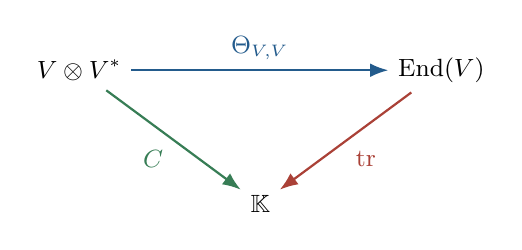
\begin{tikzpicture}[>=Latex, every node/.style={font=\small}]
 \node (tensor) at (0,1.7) {$V\otimes V^*$};
 \node (endo) at (4.6,1.7) {$\operatorname{End}(V)$};
 \node (scalar) at (2.3,0) {$\mathbb K$};
 \draw[->,thick,manifoldblue] (tensor)--node[above] {$\Theta_{V,V}$} (endo);
 \draw[->,thick,manifoldgreen] (tensor)--node[below left] {$C$} (scalar);
 \draw[->,thick,manifoldred] (endo)--node[below right] {$\operatorname{tr}$} (scalar);
\end{tikzpicture}
\caption{Kontrakcja jest śladem operatora odpowiadającego tensorowi:
$C(v\otimes\alpha)=\alpha(v)=\operatorname{tr}(w\mapsto\alpha(w)v)$.}
\label{fig:kontrakcja-slad}
\end{figure}

\begin{przyklad}[Ślad i wybór pary w kontrakcji]
Niech $S=e_1\otimes e^1+2e_2\otimes e^2$ na $\R^2$.
Wtedy $S(e_1)=e_1$, $S(e_2)=2e_2$, a $C(S)=3$.
Dla $u\otimes v\otimes\alpha\in T^2_1(V)$ kontrakcja
$v$ z $\alpha$ daje $\alpha(v)u$, zaś kontrakcja
$u$ z $\alpha$ daje $\alpha(u)v$. Wybór pary ma znaczenie:
\[
 C_{1,1}(e_1\otimes e_2\otimes e^1)=e_2,
 \qquad C_{2,1}(e_1\otimes e_2\otimes e^1)=0.
\]
Wcześniejszy tensor $P$ z przykładu typu $(1,1)$ jest niezerowy,
choć $C(P)=1-1=0$; dla $Q$ otrzymujemy $C(Q)=2$.
\end{przyklad}

\section{Algebra tensorowa i symetryzacja}
\label{sec:algebra-tensorowa}

Wyjaśnijmy użyte dalej słowa. \emph{Algebra} to przestrzeń
liniowa z dwuliniowym mnożeniem; u nas mnożenie będzie
łączne i będzie miało element jednostkowy $1$.
\emph{Suma prosta} $\bigoplus_{k\geq0}U_k$ zawiera ciągi
$(u_0,u_1,\ldots)$ z tylko skończenie wieloma niezerowymi
składnikami. \emph{Ideał obustronny} $I$ algebry $A$ to
podprzestrzeń taka, że $ai,ia\in I$ dla wszystkich
$a\in A$, $i\in I$. Dzięki temu na klasach w $A/I$
można określić mnożenie $(a+I)(b+I)=ab+I$:
zamiana $a$ na $a+i$ i $b$ na $b+j$ dodaje do
iloczynu wyrazy $aj+ib+ij\in I$. Algebra jest
\emph{stopniowana}, gdy $A=\bigoplus_{k\geq0}A^k$
i $A^kA^\ell\subseteq A^{k+\ell}$. Element należący do $A^k$ nazywamy
jednorodnym stopnia $k$. Homomorfizm algebr z jedynką to
odwzorowanie liniowe zachowujące mnożenie i jedynkę.

\begin{samepage}
\begin{definicja}[Algebra tensorowa]
\index{algebra tensorowa@Algebra tensorowa}
\label{def:algebra-tensorowa}
\emph{Algebra tensorowa} przestrzeni $V$ to suma prosta
\[
 T(V):=\bigoplus_{k=0}^{\infty}V^{\otimes k},
 \qquad V^{\otimes0}=\mathbb K.
\]
Elementy tej sumy mają tylko skończenie wiele niezerowych
składników. Mnożenie tensorów jednorodnych definiujemy przez
\emph{konkatenację}:
\[
 (v_1\otimes\cdots\otimes v_k)
 \cdot(w_1\otimes\cdots\otimes w_\ell)
 :=v_1\otimes\cdots\otimes v_k\otimes w_1\otimes\cdots\otimes w_\ell.
\]
Rozszerzamy je dwuliniowo na $T(V)$; jedynką jest $1\in\mathbb K$.
W stopniu $0$ mnożenie jest zwykłym mnożeniem przez skalar.
Na całych potęgach to mnożenie jest kanonicznym złożeniem
$V^{\otimes k}\otimes V^{\otimes\ell}\cong V^{\otimes(k+\ell)}$
ze Stwierdzenia~\ref{prop:tensor-lacznosc}; dzięki temu nie zależy
od zapisu tensorów jako sum prostych. Skończoność nośnika sum
zapewnia, że wynik znów należy do $T(V)$.
\end{definicja}
\end{samepage}

\begin{twierdzenie}[Łączność i swoboda algebry tensorowej]
\label{thm:algebra-tensorowa-universal}
$T(V)$ jest łączną algebrą z jedynką, na ogół nieprzemienną.
Dla każdej łącznej algebry $\mathcal A$ z jedynką i każdego
odwzorowania liniowego $f\colon V\to\mathcal A$ istnieje dokładnie jeden
homomorfizm algebr z jedynką $\widehat f\colon T(V)\to\mathcal A$
spełniający $\widehat f|_V=f$.
\end{twierdzenie}
\begin{proof}
Na tensorach prostych obu stron równości
$(ab)c=a(bc)$ otrzymujemy ten sam tensor przez zapisanie
wszystkich czynników po kolei. Stwierdzenie~\ref{prop:tensor-lacznosc}
pozwala pominąć nawiasy; dwuliniowość rozszerza równość
na sumy skończone. Podobnie $1\cdot a=a\cdot1=a$.

Dla ustalonego $k\geq1$ odwzorowanie
$(v_1,\ldots,v_k)\mapsto f(v_1)\cdots f(v_k)$
jest $k$-liniowe, ponieważ mnożenie w $\mathcal A$ jest
dwuliniowe. Iterowana własność uniwersalna daje jedyne odwzorowanie
liniowe $f_k\colon V^{\otimes k}\to\mathcal A$ spełniające
$f_k(v_1\otimes\cdots\otimes v_k)=f(v_1)\cdots f(v_k)$.
W stopniu $0$ kładziemy $f_0(a)=a1_{\mathcal A}$.
Definiujemy $\widehat f$ na całej sumie prostej jako sumę
$f_k$ po jej skończenie wielu niezerowych składowych.
Dla tensorów prostych zachodzi
$\widehat f(a\cdot b)=\widehat f(a)\widehat f(b)$;
dwuliniowość dowodzi tego dla dowolnych $a,b$.
Jedynka też jest zachowana. Jeśli $g$ jest drugim takim
homomorfizmem, to na $v_1\otimes\cdots\otimes v_k$
musi przyjmować wartość $g(v_1)\cdots g(v_k)
=f(v_1)\cdots f(v_k)$; te tensory i $1$ rozpinają $T(V)$.
Stąd $g=\widehat f$.
\end{proof}

\begin{przyklad}[Słowa w dwóch generatorach]
Niech $V=\R^2$ z bazą $e_1,e_2$, a
$\mathcal A=M_2(\R)$. Zadajmy liniowo
$f(e_1)=E_{12}$ i $f(e_2)=E_{21}$, gdzie $E_{ij}$ są
jednostkami macierzowymi. Własność swobodna wyznacza
$\widehat f\colon T(V)\to M_2(\R)$ i daje
\[
 \widehat f(e_1\otimes e_2)=E_{12}E_{21}=E_{11},
 \qquad
 \widehat f(e_2\otimes e_1)=E_{21}E_{12}=E_{22}.
\]
Obrazy są różne: w algebrze tensorowej kolejność liter
w iloczynie zachowuje informację.
\end{przyklad}

Dla niezależnych $e_1,e_2$ tensory $e_1\otimes e_2$ i
$e_2\otimes e_1$ są różnymi elementami $V^{\otimes2}$.
Wymuszenie przemienności prowadzi do algebry symetrycznej,
a wymuszenie $v\wedge v=0$ do algebry zewnętrznej.

\begin{definicja}[Symetryzator i antysymetryzator]
\index{symetryzator i antysymetryzator@Symetryzator i antysymetryzator}
\label{def:sym-alt}
Dla $k\geq1$ permutacja $\sigma\in S_k$ działa na
$V^{\otimes k}$ przez
\[
 P_\sigma(v_1\otimes\cdots\otimes v_k)
 :=v_{\sigma^{-1}(1)}\otimes\cdots\otimes v_{\sigma^{-1}(k)}.
\]
Odwzorowania te istnieją na mocy iterowanej własności uniwersalnej.
Definiujemy projekcje
\begin{equation}\label{eq:sym-alt}
 \operatorname{Sym}_k:=\frac1{k!}\sum_{\sigma\in S_k}P_\sigma,
 \qquad
 \operatorname{Alt}_k:=\frac1{k!}\sum_{\sigma\in S_k}
\operatorname{sgn}(\sigma)P_\sigma.
\end{equation}
W stopniu $0$ przyjmujemy
$\operatorname{Sym}_0=\operatorname{Alt}_0=\id_{\mathbb K}$.
\end{definicja}

\begin{twierdzenie}[Własności obu projekcji]
\label{thm:sym-alt}
 Zachodzą równości operatorów
\[
 \operatorname{Sym}_k^2=\operatorname{Sym}_k,\qquad
 \operatorname{Alt}_k^2=\operatorname{Alt}_k,
\]
a ich obrazy są dokładnie przestrzeniami tensorów spełniających,
odpowiednio, $P_\sigma t=t$ albo
$P_\sigma t=\operatorname{sgn}(\sigma)t$ dla każdego $\sigma$.
\end{twierdzenie}
\begin{proof}
Dzięki wyborowi $\sigma^{-1}$ w definicji
$P_\sigma\circ P_\tau=P_{\sigma\tau}$.
Istotnie, na $i$-tym miejscu po dwóch przestawieniach
stoi $v_{\tau^{-1}(\sigma^{-1}(i))}
=v_{(\sigma\tau)^{-1}(i)}$, czyli czynnik z definicji
$P_{\sigma\tau}$.
Dla ustalonej $\tau$ podstawienie
$\rho=\tau\sigma$ jest bijekcją zbioru permutacji.
W sumie symetrycznej tylko zmienia nazwy składników.
W sumie alternującej dodatkowo
$\operatorname{sgn}(\sigma)
=\operatorname{sgn}(\tau^{-1}\rho)
=\operatorname{sgn}(\tau)\operatorname{sgn}(\rho)$,
więc znak $\tau$ można wyłączyć przed sumę.
Z \eqref{eq:sym-alt} otrzymujemy zatem
\[
 P_\tau\operatorname{Sym}_k=\operatorname{Sym}_k,
 \qquad
 P_\tau\operatorname{Alt}_k
 =\operatorname{sgn}(\tau)\operatorname{Alt}_k.
\]
Tak samo, zmieniając indeks po prawej stronie, otrzymujemy
$\operatorname{Sym}_kP_\tau=\operatorname{Sym}_k$ oraz
$\operatorname{Alt}_kP_\tau=\operatorname{sgn}(\tau)\operatorname{Alt}_k$.
Każdy element pierwszego obrazu jest więc niezmienniczy,
a drugiego zmienia znak zgodnie z parzystością permutacji.
Jeżeli odwrotnie $P_\sigma t=t$ dla wszystkich $\sigma$,
to $\operatorname{Sym}_k t=\frac1{k!}\sum_\sigma t=t$.
Jeśli $P_\sigma t=\operatorname{sgn}(\sigma)t$, to
$\operatorname{Alt}_k t=
\frac1{k!}\sum_\sigma\operatorname{sgn}(\sigma)^2t=t$.
Zastosowanie projekcji do jej obrazu nic więc nie zmienia,
co daje obie równości idempotencji.
\end{proof}

Na przykład
\[
 \operatorname{Sym}_2(u\otimes v)
 =\tfrac12(u\otimes v+v\otimes u),\qquad
 \operatorname{Alt}_2(u\otimes v)
 =\tfrac12(u\otimes v-v\otimes u).
\]
Dla $u=v$ drugi tensor znika. W stopniu $k=1$ obie
projekcje są identycznością.

\begin{przyklad}[Rozkład tensora dwukowariantnego]
Niech $e_1,e_2$ będzie bazą $V$, a $e^1,e^2$ bazą dualną $V^*$; połóżmy
$t=e^1\otimes e^2+3e^2\otimes e^1$.
Wówczas $t(e_1,e_2)=1$, $t(e_2,e_1)=3$.
Transpozycja zamienia oba czynniki:
$P_{(12)}t=e^2\otimes e^1+3e^1\otimes e^2$.
W średniej $\tfrac12(t+P_{(12)}t)$ współczynniki
wynoszą $(1+3)/2=2$ i $(3+1)/2=2$,
a w różnicy $\tfrac12(t-P_{(12)}t)$ odpowiednio
$(1-3)/2=-1$ i $(3-1)/2=1$. Zatem
\[
 \operatorname{Sym}_2(t)
 =2(e^1\otimes e^2+e^2\otimes e^1),\qquad
 \operatorname{Alt}_2(t)
 =-e^1\otimes e^2+e^2\otimes e^1.
\]
Ich suma jest równa $t$. Pierwszy składnik jest symetryczny,
drugi zmienia znak po zamianie argumentów.
\end{przyklad}

Równość $t=\operatorname{Sym}_2t+\operatorname{Alt}_2t$
zachodzi dla każdego tensora drugiego stopnia, bo w sumie
$\tfrac12(\id+P_{(12)})+\tfrac12(\id-P_{(12)})$ zostaje $\id$.
Nie jest to ogólny rozkład na dwie części dla $k\geq3$.
Na przykład dla trzech niezależnych wektorów bazowych
współczynnik $e_1\otimes e_2\otimes e_3$ w
$(\operatorname{Sym}_3+\operatorname{Alt}_3)
(e_1\otimes e_2\otimes e_3)$ wynosi $2/6$, a nie $1$.

\begin{definicja}[Algebra symetryczna]
\index{algebra symetryczna@Algebra symetryczna}
\label{def:algebra-symetryczna}
Niech $J$ będzie obustronnym ideałem w $T(V)$ generowanym
przez wszystkie $u\otimes v-v\otimes u$. Iloraz
$S(V):=T(V)/J$ jest \emph{algebrą symetryczną}.
Jego składową stopnia $k$ oznaczamy $S^k(V)$.
Jest ona równa $V^{\otimes k}/(J\cap V^{\otimes k})$.
Istotnie, $J$ jest sumą swoich części jednorodnych:
w każdym elemencie $a(u\otimes v-v\otimes u)b$ rozwijamy
$a,b$ na skończone sumy składników jednorodnych. Każda
otrzymana część nadal należy do $J$. To uzasadnia stopniowanie ilorazu.
\end{definicja}

\begin{stwierdzenie}[Baza algebry symetrycznej]
\label{prop:sym-baza}
Dla bazy $e_1,\ldots,e_n$ i $k\geq0$ klasy
$e_1^{a_1}\cdots e_n^{a_n}$, gdzie
$a_i\geq0$ i $a_1+\cdots+a_n=k$, tworzą bazę $S^k(V)$.
Zatem
\[
 \dim S^k(V)=\binom{n+k-1}{k}\quad(n\geq1),
 \qquad S^k(V)\cong\operatorname{im}\operatorname{Sym}_k\quad(k\geq1).
\]
\end{stwierdzenie}
\begin{proof}
Niech $q\colon T(V)\to S(V)$ będzie ilorazem.
Ponieważ $q(e_i)q(e_j)=q(e_j)q(e_i)$, każdą klasę tensora
prostego można uporządkować do postaci
$e_1^{a_1}\cdots e_n^{a_n}$; te jednomiany rozpinają.
Zdefiniujmy homomorfizm $\pi\colon S(V)\to
\mathbb K[x_1,\ldots,x_n]$ przez $\pi(q(e_i))=x_i$.
Istnieje, bo odwzorowanie z algebry tensorowej wysyłające $e_i$
na $x_i$ zeruje każdy generator $J$. Z drugiej strony
przypisanie $x_i\mapsto q(e_i)$ wyznacza homomorfizm
$\rho\colon\mathbb K[x_1,\ldots,x_n]\to S(V)$:
na wielomianie podstawiamy za zmienne te przemienne elementy.
Oba złożenia ustalają wszystkie generatory i jedynkę,
więc są identycznościami. Niezależność i rozpinanie
wynikają teraz z niezależności zwykłych jednomianów.
Liczbę rozwiązań $a_1+\cdots+a_n=k$ otrzymujemy przez
rozmieszczenie $n-1$ przegród wśród $n+k-1$ pozycji,
czyli $\binom{n+k-1}{k}$.

Na koniec w stopniu $k$ zachodzi $q_kP_\sigma=q_k$,
zatem $q_k\operatorname{Sym}_k=q_k$. Dokładniej, permutację
można złożyć z transpozycji sąsiednich miejsc, a po takiej
zamianie klasy iloczynów są równe, bo $S(V)$ jest przemienna.
Dla $k=0,1$ mamy $J\cap V^{\otimes k}=0$.
Dla $k\ge2$ przestrzeń $J\cap V^{\otimes k}$ rozpinają elementy
\[
 a\otimes(u\otimes v-v\otimes u)\otimes b,
 \qquad a\in V^{\otimes p},\quad b\in V^{\otimes q},
 \quad p,q\ge0,\quad p+q=k-2.
\]
Tutaj $p=0$ lub $q=0$ oznacza czynnik skalarny.
Symetryzator zeruje każdy taki element: transpozycja
sąsiednich miejsc nie zmienia średniej po wszystkich
permutacjach. Przechodzi zatem
na odwzorowanie $S^k(V)\to\operatorname{im}\operatorname{Sym}_k$.
W jedną stronę jego złożenie z $q_k$ daje symetryzator,
w drugą $q_k\operatorname{Sym}_k=q_k$; są to izomorfizmy odwrotne.
Dokładniej: ograniczamy $q_k$ do obrazu symetryzatora,
na którym $\operatorname{Sym}_k$ jest identycznością.
W stopniu $0$ obie przestrzenie to $\mathbb K$ i izomorfizm
jest identycznością. Jeśli $V=0$, to $S^0(V)=\mathbb K$
i $S^k(V)=0$ dla $k>0$; wzoru z symbolem Newtona dla $n\ge1$
nie stosujemy w tym przypadku.
\end{proof}

Izomorfizm $S(V)\cong\mathbb K[x_1,\ldots,x_n]$ powyżej zależy
od wyboru bazy $e_i$. Natomiast
$S^k(V)\cong\operatorname{im}\operatorname{Sym}_k$ jest kanoniczny:
symetryzator i odwzorowanie ilorazowe nie potrzebują bazy.
Dla $V=\R^2$ odwrotność ograniczenia $q_2$ ma postać
\[
 e_1^2\longmapsto e_1\otimes e_1,\qquad
 e_1e_2\longmapsto\tfrac12(e_1\otimes e_2+e_2\otimes e_1),
 \qquad e_2^2\longmapsto e_2\otimes e_2.
\]
W szczególności klasa $e_1e_2$ w ilorazie i jej symetryczny
reprezentant w $V^{\otimes2}$ są różnymi opisami tego samego
elementu po wskazanym izomorfizmie.
Rysunek~\ref{fig:sym-iloraz} pokazuje obie drogi od tensora
do jego klasy w $S^2(V)$.
\begin{figure}[H]
\centering
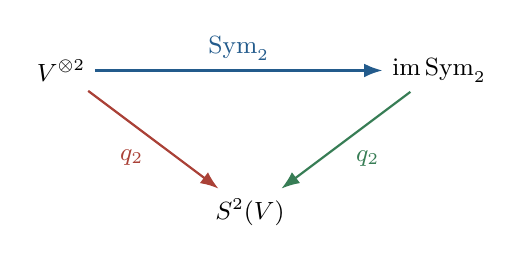
\begin{tikzpicture}[>=Latex, every node/.style={font=\small}]
 \node (tensor) at (0,1.8) {$V^{\otimes2}$};
 \node (sym) at (4.8,1.8) {$\operatorname{im}\operatorname{Sym}_2$};
 \node (quot) at (2.4,0) {$S^2(V)$};
 \draw[->,thick,manifoldblue] (tensor)--node[above] {$\operatorname{Sym}_2$} (sym);
 \draw[->,thick,manifoldred] (tensor)--node[below left] {$q_2$} (quot);
 \draw[->,thick,manifoldgreen] (sym)--node[below right] {$q_2$} (quot);
\end{tikzpicture}
\caption{Symetryzator wybiera średnią po permutacjach,
a iloraz utożsamia tensory różniące się zamianą czynników.
Prawa strzałka to ograniczenie $q_2$ do obrazu $\operatorname{Sym}_2$.
Trójkąt komutuje: $q_2\circ\operatorname{Sym}_2=q_2$.}
\label{fig:sym-iloraz}
\end{figure}

Dla $V=\R^2$ mamy np. bazę
$S^2(V)=\langle e_1^2,e_1e_2,e_2^2\rangle$,
podczas gdy $\dim V^{\otimes2}=4$. W~algebrze symetrycznej
$e_1e_2=e_2e_1$, ale w $T(V)$ odpowiednie tensory są różne.

\section{Algebra zewnętrzna i własność uniwersalna}
\label{sec:algebra-zewnetrzna}

\noindent\emph{Powiązania tematyczne w Bibliotece matematycznej:} \atlasref{LA-11::thm:lin11-zew-uniwersalna}{LA-11: własność uniwersalna algebry zewnętrznej}.


\begin{definicja}[Algebra zewnętrzna]
\index{algebra zewnetrzna@Algebra zewnętrzna}
\label{def:algebra-zewnetrzna}
Niech $I$ będzie obustronnym ideałem algebry $T(V)$
generowanym przez $v\otimes v$ dla wszystkich $v\in V$.
\emph{Algebra zewnętrzna} jest ilorazem
\[
 \Lambda(V):=T(V)/I,
 \qquad \Lambda^k(V):=V^{\otimes k}/(I\cap V^{\otimes k}).
\]
Iloczyn w ilorazie zapisujemy $\wedge$, a obraz
$v_1\otimes\cdots\otimes v_k$ oznaczamy
$v_1\wedge\cdots\wedge v_k$.
\end{definicja}

Iloraz wymusza, by dwukrotne użycie tego samego kierunku
dawało zero. Po rozwinięciu kwadratu $u+v$ będzie to oznaczało,
że zamiana dwóch sąsiednich wektorów zmienia znak.
Tak powstaje algebra uwzględniająca kolejność i orientację
kierunków, odmienna od algebry słów $T(V)$.

Ideał $I$ jest jednorodny: jego generatory mają stopień $2$,
a każdy iloczyn z tensorami jednorodnymi ma określony stopień.
Stąd podana definicja $\Lambda^k(V)$ jest zgodna z rozkładem
$\Lambda(V)=\bigoplus_{k\geq0}\Lambda^k(V)$.
W stopniach $0$ i $1$ ideał nie ma elementów niezerowych, dlatego
$\Lambda^0(V)=\mathbb K$ i $\Lambda^1(V)=V$.

\begin{stwierdzenie}[Relacje i znaki]
\label{prop:wedge-znak}
W $\Lambda(V)$ zachodzą
\begin{equation}\label{eq:wedge-relacje}
 v\wedge v=0,\qquad u\wedge v=-v\wedge u.
\end{equation}
Jeżeli $\alpha\in\Lambda^k(V)$ i $\beta\in\Lambda^\ell(V)$,
to
\begin{equation}\label{eq:wedge-graded}
 \alpha\wedge\beta=(-1)^{k\ell}\beta\wedge\alpha.
\end{equation}
Mnożenie $\wedge$ jest dwuliniowe, łączne i ma jedynkę $1$.
\end{stwierdzenie}
\begin{proof}
Pierwsza równość~\eqref{eq:wedge-relacje} jest relacją
z definicji ideału. Po podstawieniu $u+v$ dostajemy
$0=(u+v)\wedge(u+v)=u\wedge v+v\wedge u$;
stąd druga równość. Iloraz algebry łącznej z jedynką przez
ideał obustronny dziedziczy łączność i dwuliniowość.
Ponieważ ideał składa się z elementów stopni co najmniej $2$,
nie zawiera jedynki i jej klasa pozostaje jedynką.

Dla prostych $\alpha=v_1\wedge\cdots\wedge v_k$ i
$\beta=w_1\wedge\cdots\wedge w_\ell$ przejście od
$\alpha\wedge\beta$ do $\beta\wedge\alpha$ wymaga
$k\ell$ zamian miejsc sąsiednich wektorów. Każda zamiana
zmienia znak, co dowodzi~\eqref{eq:wedge-graded} dla
prostych wielowektorów. Te rozpinają składowe jednorodne,
a dwuliniowość kończy dowód.
Gdy $k=0$ lub $\ell=0$, wzór wynika też bezpośrednio
z działania skalarów: każdy element $\Lambda^0(V)=\mathbb K$
jest wielokrotnością jedynki.
\end{proof}

Na przykład dla trzech niezależnych wektorów
$e_1,e_2,e_3$ mamy $e_1\wedge e_2=-e_2\wedge e_1$,
ale
\[
 (e_1\wedge e_2)\wedge e_3
 =e_3\wedge(e_1\wedge e_2).
\]
Przesunięcie $e_3$ przez dwa czynniki daje znak
$(-1)^{2\cdot1}=+1$.

\begin{twierdzenie}[Własność uniwersalna algebry zewnętrznej]
\label{thm:wedge-algebra-universal}
Niech $\mathcal A$ będzie łączną algebrą z jedynką,
a $f\colon V\to\mathcal A$ odwzorowaniem liniowym takim, że
$f(v)^2=0$ dla każdego $v\in V$. Istnieje dokładnie jeden
homomorfizm algebr z jedynką
$\bar f\colon\Lambda(V)\to\mathcal A$ spełniający
$\bar f(v)=f(v)$ dla $v\in\Lambda^1(V)=V$.
\end{twierdzenie}
\begin{proof}
Z Twierdzenia~\ref{thm:algebra-tensorowa-universal} mamy
jedyny homomorfizm $\widehat f\colon T(V)\to\mathcal A$
przedłużający $f$. Dla każdego generatora ideału $I$
zachodzi $\widehat f(v\otimes v)=f(v)^2=0$.
Warunek ten oznacza także antykomutację obrazów:
\[
 0=f(u+v)^2=f(u)f(v)+f(v)f(u),
\]
bo kwadraty $f(u)^2$ i $f(v)^2$ są zerowe.
Jądro homomorfizmu jest ideałem obustronnym, więc zawiera
cały $I$. Odwzorowanie
$\bar f([t]):=\widehat f(t)$ na $T(V)/I$ jest zatem
dobrze określone i jest homomorfizmem. Każdy homomorfizm
przedłużający $f$ musi na klasie
$v_1\wedge\cdots\wedge v_k$ przyjmować wartość
$f(v_1)\cdots f(v_k)$; te klasy wraz z jedynką rozpinają
$\Lambda(V)$. Stąd jednoznaczność.
\end{proof}

\begin{przyklad}[Przedłużenie odwzorowania liniowego]
Niech $V=\R^2$ z bazą $e_1,e_2$ i $W=\R^2$ z bazą
$a,b$. Zadajmy $f\colon V\to\Lambda(W)$ przez
$f(e_1)=a$, $f(e_2)=2b$. Każdy $f(v)$ ma stopień $1$,
więc $f(v)\wedge f(v)=0$. Twierdzenie daje homomorfizm
$\bar f\colon\Lambda(V)\to\Lambda(W)$, dla którego
$\bar f(1)=1$ i
\[
 \bar f(e_1\wedge e_2)=f(e_1)\wedge f(e_2)=2a\wedge b.
\]
Wartość na pozostałych iloczynach wyznaczają liniowość
i mnożenie, bez wyboru dodatkowych reguł.
\end{przyklad}

Przypomnijmy związek alternowania ze znakiem. Jeśli odwzorowanie
wieloliniowe $b$ znika przy powtórzeniu argumentów, to rozwinięcie
$0=b(\ldots,u+v,\ldots,u+v,\ldots)$ w dwóch wskazanych miejscach
daje
\[
 b(\ldots,u,\ldots,v,\ldots)
 =-b(\ldots,v,\ldots,u,\ldots).
\]
Wyrazy z dwoma $u$ i dwoma $v$ znikają. Każda permutacja jest
złożeniem transpozycji, więc przestawienie argumentów mnoży wynik
przez jej znak. Odwrotnie, zmiana znaku przy każdej transpozycji
daje $b=-b$ przy równych argumentach, czyli $b=0$ nad $\R$ lub $\C$.
Stąd w tym rozdziale „alternujący” i „antysymetryczny” są równoważne
dla odwzorowań wieloliniowych.

\begin{twierdzenie}[Własność uniwersalna stopnia $k$]
\label{thm:wedge-multilinear}
Dla $k\geq1$ odwzorowanie
\[
 (v_1,\ldots,v_k)\longmapsto v_1\wedge\cdots\wedge v_k
\]
jest $k$-liniowe i alternujące: znika, gdy dwa jego argumenty
są równe. Dla każdej przestrzeni $Z$ i każdego alternującego
$k$-liniowego odwzorowania $b\colon V^k\to Z$ istnieje dokładnie jedno
odwzorowanie liniowe $\bar b\colon\Lambda^k(V)\to Z$ takie, że
\[
 \bar b(v_1\wedge\cdots\wedge v_k)=b(v_1,\ldots,v_k).
\]
\end{twierdzenie}
\begin{proof}
Wieloliniowość wynika z definicji mnożenia i z liniowej
inkluzji $V=\Lambda^1(V)$. Jeśli dwa wektory są równe,
przesuwamy jeden przez sąsiednie czynniki, korzystając
z~\eqref{eq:wedge-relacje}, aż znajdą się obok siebie.
Wtedy ich iloczyn jest zerowy.

Przez iterowaną własność iloczynu tensorowego odwzorowanie $b$
wyznacza jedyne odwzorowanie liniowe
$\widetilde b\colon V^{\otimes k}\to Z$ z
$\widetilde b(v_1\otimes\cdots\otimes v_k)=b(v_1,\ldots,v_k)$.
Jednorodna część $I\cap V^{\otimes k}$ jest rozpięta
przez elementy postaci
$x\otimes v\otimes v\otimes y$, gdzie $x,y$ są tensorami
prostymi (dopuszczamy skalar w stopniu $0$), a łączny stopień
wynosi $k$. Na każdym z nich
$\widetilde b$ znika, bo w $b$ występują dwa jednakowe
argumenty. Wobec tego $\widetilde b$ przechodzi na iloraz
$\Lambda^k(V)$ i określa $\bar b$.
Wielowektory proste rozpinają ten iloraz, więc faktoryzacja
jest jednoznaczna.
\end{proof}

\begin{przyklad}[Wyznacznik na drugiej potędze zewnętrznej]
Na $V=\R^2$ funkcja $b(v,w)=\det(v,w)$ jest dwuliniowa
i alternująca. Własność uniwersalna daje jedyne liniowe
$\bar b\colon\Lambda^2(\R^2)\to\R$ z
$\bar b(v\wedge w)=\det(v,w)$.
Ponieważ $\bar b(e_1\wedge e_2)=1$, wielowektor
$e_1\wedge e_2$ nie jest zerowy. W
Sekcji~\ref{sec:iloczyn-tensorowy} ten sam
wyznacznik działał na całym $V\otimes V$;
tutaj dodatkowo przechodzi przez iloraz, bo
$\det(v,v)=0$.
\end{przyklad}

\begin{twierdzenie}[Antysymetryzacja a iloczyn zewnętrzny]
\label{thm:wedge-alt}
Niech $q_k\colon V^{\otimes k}\to\Lambda^k(V)$ będzie odwzorowaniem
ilorazowym. Istnieje kanoniczny izomorfizm
\[
 j_k\colon\Lambda^k(V)\longrightarrow
 \operatorname{im}\operatorname{Alt}_k\subseteq V^{\otimes k},
 \qquad j_k(v_1\wedge\cdots\wedge v_k)
 =\operatorname{Alt}_k(v_1\otimes\cdots\otimes v_k).
\]
W szczególności $j_2(u\wedge v)=
\tfrac12(u\otimes v-v\otimes u)$. Przy tym utożsamieniu,
dla tensorów antysymetrycznych $a$ stopnia $k$ i $b$ stopnia
$\ell$ ich iloczyn zewnętrzny odpowiada
$\operatorname{Alt}_{k+\ell}(a\otimes b)$.
\end{twierdzenie}
\begin{proof}
Jeżeli tensor prosty zawiera kolejno $v\otimes v$, to
transpozycja tych dwóch miejsc pozostawia go bez zmian,
ale zmienia znak jego antysymetryzacji zgodnie z
Twierdzeniem~\ref{thm:sym-alt}. Ponieważ pracujemy nad
$\R$ lub $\C$, jego antysymetryzacja jest zerowa.
To samo dotyczy wielokrotności i sum takich tensorów,
zatem $\operatorname{Alt}_k$ zeruje $I\cap V^{\otimes k}$
i przechodzi na wskazane odwzorowanie $j_k$.

W ilorazie permutacja czynników zmienia znak o
$\operatorname{sgn}(\sigma)$, na mocy~\eqref{eq:wedge-relacje}.
Dla wielowektora prostego mamy więc
\[
 q_kj_k(v_1\wedge\cdots\wedge v_k)
 =\frac1{k!}\sum_{\sigma\in S_k}
 \operatorname{sgn}(\sigma)^2
 (v_1\wedge\cdots\wedge v_k)
 =v_1\wedge\cdots\wedge v_k.
\]
Wynika stąd iniektywność $j_k$. Z drugiej strony
$j_kq_k=\operatorname{Alt}_k$ na tensorach prostych,
a więc wszędzie, co dowodzi surjektywności na obraz.
Jeśli $a=j_k(\alpha)$ i $b=j_\ell(\beta)$, to
$j_{k+\ell}(\alpha\wedge\beta)
=\operatorname{Alt}_{k+\ell}(a\otimes b)$,
bo $q_k(a)=\alpha$, $q_\ell(b)=\beta$ i stosujemy właśnie
sprawdzoną równość $j_{k+\ell}q_{k+\ell}=\operatorname{Alt}_{k+\ell}$.
\end{proof}

\begin{uwaga}[Skąd bierze się czynnik $1/k!$?]
\label{rem:normalizacja-wedge}
Obraz $u\wedge v$ w \emph{algebrze zewnętrznej} to klasa
$u\otimes v$. Dopiero jego kanoniczny reprezentant w
\emph{przestrzeni tensorów antysymetrycznych}, dany przez $j_2$,
ma postać $\tfrac12(u\otimes v-v\otimes u)$. W szczególności
nie wolno utożsamiać tych dwóch zapisów bez podania
normalizacji. Sprawdzenie w ilorazie daje
\[
 q_2\!\left(\tfrac12(u\otimes v-v\otimes u)\right)
 =\tfrac12(u\wedge v-v\wedge u)=u\wedge v.
\]
Dla kowektorów standardowe odwzorowanie
$\Lambda^k(V^*)$ na funkcje alternujące na $V^k$
przyjmiemy z normalizacją przez wyznacznik w
Sekcji~\ref{sec:wyznacznik}.
\end{uwaga}

\section{Baza i wymiar potęg zewnętrznych}
\label{sec:baza-zewnetrzna}

\begin{twierdzenie}[Baza potęgi zewnętrznej]
\label{thm:wedge-baza}
Niech $e_1,\ldots,e_n$ będzie bazą $V$. Dla $0\leq k\leq n$
rodzina
\[
 e_{i_1}\wedge\cdots\wedge e_{i_k},
 \qquad 1\leq i_1<\cdots<i_k\leq n,
\]
stanowi bazę $\Lambda^k(V)$; dla $k=0$ jest to wektor $1$.
Dla $k>n$ zachodzi $\Lambda^k(V)=0$. W szczególności
\begin{equation}\label{eq:wedge-wymiar}
 \dim\Lambda^k(V)=\binom nk,\qquad
 \dim\Lambda(V)=\sum_{k=0}^n\binom nk=2^n.
\end{equation}
\end{twierdzenie}
\begin{proof}
Jeśli $k=0$, mamy $\Lambda^0(V)=\mathbb K$ z bazą $\{1\}$.
Dalej niech $k\geq1$.
Rozwijamy każdy czynnik $v_a$ w bazie $e_i$ i korzystamy
z wieloliniowości iloczynu zewnętrznego. Otrzymujemy sumę
wielowektorów $e_{j_1}\wedge\cdots\wedge e_{j_k}$.
Jeśli indeks się powtarza, składnik znika, bo dwa jednakowe
wektory można ustawić obok siebie. Pozostałe porządkujemy
rosnąco, a każda zamiana sąsiadów daje minus. Rodzina
z tezy rozpięła więc $\Lambda^k(V)$; dla $k>n$ wszystkie
ciągi $k$ indeksów mają powtórzenie, więc
cała przestrzeń jest zerowa.

Dla $1\leq k\leq n$ udowodnimy niezależność;
nie wystarczy do tego samo porządkowanie.
Dla rosnącego indeksu $I=(i_1<\cdots<i_k)$ i
$v_b=\sum_j a_{jb}e_j$ definiujemy
\begin{equation}\label{eq:wedge-wspolrzedne-minor}
 D_I(v_1,\ldots,v_k)
 :=\sum_{\sigma\in S_k}\operatorname{sgn}(\sigma)
 \prod_{b=1}^k a_{i_{\sigma(b)},b}.
\end{equation}
W każdym składniku dla ustalonego $b$ występuje dokładnie
jeden współczynnik wektora $v_b$, więc $D_I$ jest
wieloliniowa. Zamiana dwóch argumentów przestawia dwie
kolumny: permutacje w sumie parują się ze znakami przeciwnymi.
Dlatego $D_I$ jest alternująca. Własność uniwersalna z
Twierdzenia~\ref{thm:wedge-multilinear} daje funkcjonał
$\overline D_I\colon\Lambda^k(V)\to\mathbb K$.
Na uporządkowanym wielowektorze bazowym $e_{j_1}\wedge\cdots
\wedge e_{j_k}$ wartość $\overline D_I$ wynosi $1$,
gdy $I=(j_1,\ldots,j_k)$, oraz $0$ w przeciwnym razie.
Jeżeli zatem suma $\sum_J c_J e_{j_1}\wedge\cdots\wedge e_{j_k}$
jest zerowa, zastosowanie kolejno $\overline D_I$ daje
$c_I=0$ dla każdego $I$. Rodzina jest liniowo niezależna.
Indeksów rosnących długości $k$ jest $\binom nk$;
sumę wymiarów obliczamy z dwumianu Newtona.
Ponieważ $\overline D_I$ odczytuje współczynnik przy $e_I$,
otrzymujemy także jawny wzór współrzędnych
\begin{equation}\label{eq:wedge-rozwiniecie-minory}
 v_1\wedge\cdots\wedge v_k
 =\sum_{1\leq i_1<\cdots<i_k\leq n}
 D_{(i_1,\ldots,i_k)}(v_1,\ldots,v_k)
 e_{i_1}\wedge\cdots\wedge e_{i_k}.
\end{equation}
\end{proof}

\begin{przyklad}[Współczynniki $u\wedge v$]
Dla $V=\R^3$, $u=e_1+2e_2$ i $v=e_2+e_3$ mamy
\[
 u\wedge v=(e_1+2e_2)\wedge(e_2+e_3)
 =e_1\wedge e_2+e_1\wedge e_3+2e_2\wedge e_3.
\]
Współczynnik przy $e_i\wedge e_j$ jest wyznacznikiem
$\begin{psmallmatrix}u^i&v^i\\u^j&v^j\end{psmallmatrix}
=u^iv^j-u^jv^i$, zgodnie z~\eqref{eq:wedge-rozwiniecie-minory}.
Tutaj macierz dwóch kolumn ma postać
\[
 [u\ v]=\begin{pmatrix}1&0\\2&1\\0&1\end{pmatrix}.
\]
Jej trzy minory wierszy $(1,2)$, $(1,3)$ i $(2,3)$
wynoszą odpowiednio $1$, $1$ i $2$; są dokładnie trzema
współczynnikami w otrzymanym rozwinięciu $u\wedge v$.
\end{przyklad}

W standardowej euklidesowej $\R^3$ minory można odczytać
jako zorientowane pola rzutów ortogonalnych równoległoboku rozpiętego
przez $(u,v)$ na trzy płaszczyzny współrzędnych.
Rysunek~\ref{fig:wedge-minory-rzuty} przedstawia rzuty
z powyższego przykładu w tej samej skali.
\begin{figure}[H]
\centering
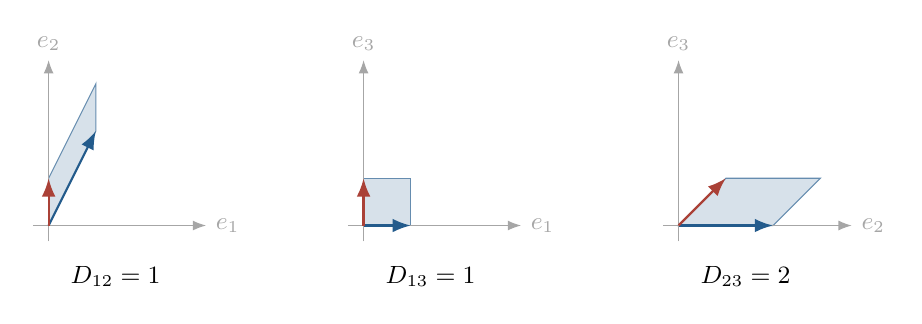
\begin{tikzpicture}[>=Latex, every node/.style={font=\small}]
 \begin{scope}[xshift=-4cm]
  \fill[manifoldblue!18] (0,0)--(.6,1.2)--(.6,1.8)--(0,.6)--cycle;
  \draw[manifoldblue!70] (0,0)--(.6,1.2)--(.6,1.8)--(0,.6)--cycle;
  \draw[gray!70,->] (-.2,0)--(2,0) node[right] {$e_1$};
  \draw[gray!70,->] (0,-.2)--(0,2.1) node[above] {$e_2$};
  \draw[manifoldblue,thick,->] (0,0)--(.6,1.2);
  \draw[manifoldred,thick,->] (0,0)--(0,.6);
  \node at (.85,-.65) {$D_{12}=1$};
 \end{scope}
 \begin{scope}
  \fill[manifoldblue!18] (0,0)--(.6,0)--(.6,.6)--(0,.6)--cycle;
  \draw[manifoldblue!70] (0,0)--(.6,0)--(.6,.6)--(0,.6)--cycle;
  \draw[gray!70,->] (-.2,0)--(2,0) node[right] {$e_1$};
  \draw[gray!70,->] (0,-.2)--(0,2.1) node[above] {$e_3$};
  \draw[manifoldblue,thick,->] (0,0)--(.6,0);
  \draw[manifoldred,thick,->] (0,0)--(0,.6);
  \node at (.85,-.65) {$D_{13}=1$};
 \end{scope}
 \begin{scope}[xshift=4cm]
  \fill[manifoldblue!18] (0,0)--(1.2,0)--(1.8,.6)--(.6,.6)--cycle;
  \draw[manifoldblue!70] (0,0)--(1.2,0)--(1.8,.6)--(.6,.6)--cycle;
  \draw[gray!70,->] (-.2,0)--(2.2,0) node[right] {$e_2$};
  \draw[gray!70,->] (0,-.2)--(0,2.1) node[above] {$e_3$};
  \draw[manifoldblue,thick,->] (0,0)--(1.2,0);
  \draw[manifoldred,thick,->] (0,0)--(.6,.6);
  \node at (.85,-.65) {$D_{23}=2$};
 \end{scope}
\end{tikzpicture}
\caption{Rzuty równoległoboku $(u,v)$ na płaszczyzny
rozpięte przez $(e_1,e_2)$, $(e_1,e_3)$ i $(e_2,e_3)$
w standardowej $\R^3$.
Niebieska strzałka to rzut $u$, czerwona to rzut $v$;
zorientowane pola rzutów wynoszą odpowiednio $1,1,2$.}
\label{fig:wedge-minory-rzuty}
\end{figure}

\begin{przyklad}[Nie każdy dwuwektor jest prosty]
W $\Lambda^2(\R^4)$ weźmy
$\omega=e_1\wedge e_2+e_3\wedge e_4$. Wówczas
\[
\begin{aligned}
 \omega\wedge\omega
 &=(e_1\wedge e_2)\wedge(e_3\wedge e_4)
   +(e_3\wedge e_4)\wedge(e_1\wedge e_2)\\
 &=2e_1\wedge e_2\wedge e_3\wedge e_4\ne0.
\end{aligned}
\]
Oba kwadraty składników prostych znikają, a dwa składniki
mieszane są równe, ponieważ zamiana bloków stopni $2$ i $2$
daje znak $(-1)^{2\cdot2}=+1$.
Natomiast $(u\wedge v)\wedge(u\wedge v)=0$ dla każdego
$u,v$, gdyż $u$ występuje dwa razy. Zatem $\omega$ nie
jest pojedynczym iloczynem $u\wedge v$. Pokazuje to, że
również w algebrze zewnętrznej potrzebujemy sum wielowektorów
prostych.
\end{przyklad}

\section{Potęgi zewnętrzne i wyznacznik}
\label{sec:wyznacznik}

\noindent\emph{Powiązania tematyczne w Bibliotece matematycznej:} \atlasref{LA-11::thm:lin11-det-wedge}{LA-11: wyznacznik a najwyższa potęga zewnętrzna}.


Iloczyn $v_1\wedge\cdots\wedge v_k$ zapisuje
antysymetryczną informację o $k$ wektorach. W standardowej $\R^n$
jego współczynniki opisują zorientowane objętości
rzutów na płaszczyzny współrzędnych. Odwzorowanie liniowe
przenosi każdy wektor, a więc także ich iloczyn; macierz
działania na wielowektorach ma w odpowiednich bazach minory
jako współczynniki. Dla operatora
$A\colon V\to V$ i $k=n=\dim V$ przestrzeń $\Lambda^n(V)$
jest jednowymiarowa, więc pozostaje jeden skalar: wyznacznik.

\begin{twierdzenie}[Potęga zewnętrzna odwzorowania]
\label{thm:potega-zewn-operatora}
Dla liniowego $A\colon V\to W$ i $k\geq1$ istnieje dokładnie jedno odwzorowanie
liniowe
\[
 \Lambda^k A\colon\Lambda^k(V)\to\Lambda^k(W),\qquad
 (\Lambda^k A)(v_1\wedge\cdots\wedge v_k)
 =Av_1\wedge\cdots\wedge Av_k.
\]
Dla $B\colon W\to U$ zachodzi
$\Lambda^k(B\circ A)=\Lambda^k B\circ\Lambda^k A$
i $\Lambda^k\id_V=\id_{\Lambda^k(V)}$.
Przyjmujemy również $\Lambda^0A=\id_{\mathbb K}$; wtedy powyższe
prawa obowiązują także dla $k=0$, a pusty iloczyn zewnętrzny oznacza $1$.
\end{twierdzenie}
\begin{proof}
Odwzorowanie $(v_1,\ldots,v_k)\mapsto
Av_1\wedge\cdots\wedge Av_k$ jest wieloliniowe,
bo $A$ jest liniowe, a iloczyn zewnętrzny wieloliniowy.
Gdy dwa argumenty są równe, odpowiadające im obrazy też
są równe, więc iloczyn znika. Twierdzenie~\ref{thm:wedge-multilinear}
daje jedyne odwzorowanie $\Lambda^k A$.
Na wielowektorze prostym obie strony wzoru na złożenie
dają $BA v_1\wedge\cdots\wedge BA v_k$.
Wielowektory proste rozpinają $\Lambda^k(V)$, co dowodzi
równości na całej przestrzeni. Argument dla identyczności
jest taki sam.
\end{proof}

\begin{definicja}[Wyznacznik operatora]
\index{wyznacznik operatora@Wyznacznik operatora}
\label{def:det-wedge}
Jeżeli $\dim V=n$, to $\Lambda^n(V)$ jest jednowymiarowa
na mocy Twierdzenia~\ref{thm:wedge-baza}. Dla operatora
$A\colon V\to V$ jego \emph{wyznacznik} jest jedynym skalarem
$\det A\in\mathbb K$, dla którego
\begin{equation}\label{eq:det-top-wedge}
 \Lambda^n A=(\det A)\id_{\Lambda^n(V)}.
\end{equation}
Dla $V=0$ przyjmujemy $\det\id_V=1$; odpowiada temu
wyznacznik pustej macierzy równy $1$.
\end{definicja}

\begin{twierdzenie}[Wzór Leibniza i własności wyznacznika]
\label{thm:det-wlasnosci}
Jeśli $Ae_j=\sum_{i=1}^n a_{ij}e_i$, to
\begin{equation}\label{eq:det-leibniz}
 \det A=\sum_{\sigma\in S_n}\operatorname{sgn}(\sigma)
 \prod_{j=1}^n a_{\sigma(j),j}.
\end{equation}
Ponadto
\[
 \det\id_V=1,\qquad \det(B\circ A)=\det B\,\det A,
 \qquad \det A\ne0\ \Longleftrightarrow\ A\text{ jest odwracalne}.
\]
Wartość $\det A$ nie zależy od bazy; wyznacznik jest
liniowy w każdej kolumnie macierzy i zmienia znak po
zamianie dwóch kolumn.
\end{twierdzenie}
\begin{proof}
Niech $\varepsilon=e_1\wedge\cdots\wedge e_n\ne0$.
Z~\eqref{eq:det-top-wedge} i wieloliniowości mamy
\[
 (\det A)\varepsilon
 =Ae_1\wedge\cdots\wedge Ae_n
 =\sum_{i_1,\ldots,i_n}
   a_{i_1,1}\cdots a_{i_n,n}
   e_{i_1}\wedge\cdots\wedge e_{i_n}.
\]
Wyrazy z powtarzającym się indeksem znikają. Pozostałe
ciągi $(i_1,\ldots,i_n)$ są permutacjami
$(\sigma(1),\ldots,\sigma(n))$, a przestawienie odpowiadającego
iloczynu zewnętrznego do $\varepsilon$ daje znak
$\operatorname{sgn}(\sigma)$. Porównanie współczynników
przy niezerowym $\varepsilon$ daje~\eqref{eq:det-leibniz}.

Twierdzenie~\ref{thm:potega-zewn-operatora} w stopniu $n$
daje $\Lambda^n(B\circ A)=\Lambda^n B\circ\Lambda^n A$.
Ponieważ każde z tych odwzorowań jest mnożeniem przez odpowiedni
skalar, otrzymujemy $\det(BA)=\det B\det A$;
tak samo $\det\id_V=1$. Jeśli $A$ ma odwrotność,
$1=\det(A^{-1}A)=\det(A^{-1})\det A$, więc $\det A\ne0$.
Jeżeli $A$ nie ma odwrotności, kolumny $Ae_1,\ldots,Ae_n$
są liniowo zależne. Jedna z nich jest kombinacją pozostałych,
a po rozwinięciu odpowiadającego czynnika każdy wyraz
$Ae_1\wedge\cdots\wedge Ae_n$ zawiera powtórzony wektor
i znika. Stąd $\det A=0$.

Definicja~\eqref{eq:det-top-wedge} mówi o skalarze działania
operatora na samej jednowymiarowej przestrzeni
$\Lambda^n(V)$, dlatego nie zależy od wyboru jej bazy.
Wreszcie $Ae_1\wedge\cdots\wedge Ae_n$ jest liniowy
w każdym czynniku i antysymetryczny przy ich zamianie;
jego współczynnik przy $\varepsilon$, czyli wyznacznik,
ma takie same własności względem kolumn.
\end{proof}

\begin{przyklad}[Pole zorientowane w $\R^2$]
Niech $u=(3,1)$ i $v=(1,2)$ w standardowej bazie.
Wówczas
\[
 u\wedge v=(3e_1+e_2)\wedge(e_1+2e_2)
 =(3\cdot2-1\cdot1)e_1\wedge e_2
 =5e_1\wedge e_2.
\]
Wartość $5$ jest polem równoległoboku ze znakiem określonym
przez kolejność $(u,v)$; pole geometryczne wynosi $|5|$.
Zmiana kolejności wektorów daje $v\wedge u=-5e_1\wedge e_2$.
Para $(u,v)$ ma tu orientację dodatnią względem $(e_1,e_2)$.
\end{przyklad}

\begin{figure}[H]
\centering
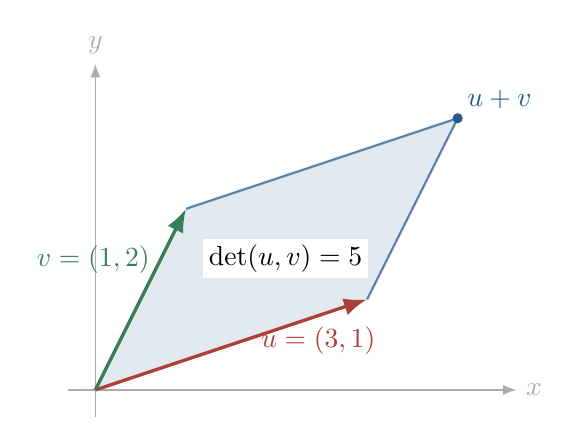
\begin{tikzpicture}[>=Latex,scale=1.15]
 \coordinate (O) at (0,0);
 \coordinate (U) at (3,1);
 \coordinate (V) at (1,2);
 \coordinate (UV) at (4,3);
 \fill[manifoldblue!13] (O)--(U)--(UV)--(V)--cycle;
 \draw[->,gray!65] (-0.3,0)--(4.65,0) node[right] {$x$};
 \draw[->,gray!65] (0,-0.3)--(0,3.6) node[above] {$y$};
 \draw[thick,manifoldblue!75] (U)--(UV)--(V);
 \draw[->,very thick,manifoldred] (O)--(U)
   node[pos=0.82,below] {$u=(3,1)$};
 \draw[->,very thick,manifoldgreen] (O)--(V)
   node[pos=0.72,left] {$v=(1,2)$};
 \fill[manifoldblue] (UV) circle (1.6pt) node[above right] {$u+v$};
 \node[fill=white,inner sep=2pt] at (2.1,1.45)
   {$\det(u,v)=5$};
\end{tikzpicture}
\caption{Iloczyn zewnętrzny w $\R^2$ koduje pole i orientację
równoległoboku. Zmiana kolejności wektorów zmienia znak.}
\label{fig:wedge-pole}
\end{figure}

\begin{twierdzenie}[Minory jako macierz $\Lambda^k A$]
\label{thm:minory-lambda}
Niech $A\colon\mathbb K^n\to\mathbb K^m$ ma macierz
$(a_{ij})$. W bazach uporządkowanych z
Twierdzenia~\ref{thm:wedge-baza} współczynnik macierzy
$\Lambda^k A$ w wierszu $I=(i_1<\cdots<i_k)$ i kolumnie
$J=(j_1<\cdots<j_k)$ jest wyznacznikiem podmacierzy
$A_{I,J}=(a_{i_a,j_b})_{a,b=1}^k$.
\end{twierdzenie}
\begin{proof}
Rozwijamy
$Ae_{j_1}\wedge\cdots\wedge Ae_{j_k}$ według
$Ae_{j_b}=\sum_i a_{i,j_b}e_i$. Przy bazowym
$e_{i_1}\wedge\cdots\wedge e_{i_k}$ pojawiają się tylko
składniki, których $k$ indeksów stanowi permutację $I$.
Po ustawieniu ich w kolejności rosnącej dostajemy
\[
 \sum_{\sigma\in S_k}\operatorname{sgn}(\sigma)
 \prod_{b=1}^k a_{i_{\sigma(b)},j_b}
 =\det A_{I,J}
\]
na mocy wzoru~\eqref{eq:det-leibniz} dla macierzy $k\times k$.
Nie występują żadne inne składniki przy wskazanym
wektorze bazowym, więc to jest szukany współczynnik.
\end{proof}

\begin{wniosek}[Wzór Cauchy'ego--Bineta]
\label{cor:cauchy-binet}
Dla macierzy $A$ o wymiarach $m\times n$ i $B$ o wymiarach
$n\times p$, oraz rosnących indeksów $I\subseteq\{1,\ldots,m\}$,
$J\subseteq\{1,\ldots,p\}$ długości $k$, gdzie $0\leq k\leq\min(m,p)$,
zachodzi
\begin{equation}\label{eq:cauchy-binet}
 \det\bigl((AB)_{I,J}\bigr)
 =\sum_{\substack{K\subseteq\{1,\ldots,n\}\\ |K|=k}}
 \det A_{I,K}\,\det B_{K,J}.
\end{equation}
\end{wniosek}
\begin{proof}
Z Twierdzenia~\ref{thm:potega-zewn-operatora} mamy
$\Lambda^k(AB)=(\Lambda^k A)(\Lambda^k B)$.
Twierdzenie~\ref{thm:minory-lambda} mówi, że macierze
trzech występujących tu operatorów mają za współczynniki
odpowiednie minory. Współczynnik iloczynu macierzy w
wierszu $I$ i kolumnie $J$ to suma po wszystkich
$k$-elementowych indeksach pośrednich $K$; jest ona
dokładnie prawą stroną~\eqref{eq:cauchy-binet}.
Dla $k=0$ obie strony są równe $1$. Gdy $k>n$,
nie ma indeksów $K$ i suma jest zerowa, zgodnie z tym,
że $\Lambda^k(\mathbb K^n)=0$.
\end{proof}

\begin{przyklad}[Obliczenie wzoru Cauchy'ego--Bineta]
Niech
\[
 A=\begin{pmatrix}1&2&0\\0&1&1\end{pmatrix},\qquad
 B=\begin{pmatrix}1&0\\0&1\\1&2\end{pmatrix}.
\]
Macierze $\Lambda^2A\colon\Lambda^2\R^3\to\Lambda^2\R^2$
i $\Lambda^2B\colon\Lambda^2\R^2\to\Lambda^2\R^3$ mają,
w uporządkowaniu indeksów $12,13,23$, odpowiednio postacie
\[
 [\Lambda^2A]=\begin{pmatrix}1&1&2\end{pmatrix},\qquad
 [\Lambda^2B]=\begin{pmatrix}1\\2\\-1\end{pmatrix}.
\]
Na przykład minor $A_{\{1,2\},\{2,3\}}$ wynosi
$\det\bigl(\begin{smallmatrix}2&0\\1&1\end{smallmatrix}\bigr)=2$,
a minor $B_{\{2,3\},\{1,2\}}$ wynosi
$\det\bigl(\begin{smallmatrix}0&1\\1&2\end{smallmatrix}\bigr)=-1$.
Zatem $\det(AB)=1\cdot1+1\cdot2+2\cdot(-1)=1$.
Bezpośrednio $AB=\bigl(\begin{smallmatrix}1&2\\1&3\end{smallmatrix}\bigr)$,
również o wyznaczniku $1$. Wzór sumuje wkłady trzech
możliwych płaszczyzn współrzędnych przestrzeni pośredniej $\R^3$;
ich znaki mogą się znosić.
\end{przyklad}

Oznaczamy przez $\operatorname{Alt}^k(V;\mathbb K)$ przestrzeń
alternujących $k$-liniowych funkcji $V^k\to\mathbb K$.
Dla $k=0$ jest to $\mathbb K$.

\begin{twierdzenie}[Kowektory zewnętrzne jako odwzorowania alternujące]
\label{thm:dual-zewnetrzny}
Dla skończenie wymiarowego $V$ istnieje kanoniczny izomorfizm
\[
 \mathcal E_k\colon\Lambda^k(V^*)
 \longrightarrow\operatorname{Alt}^k(V;\mathbb K),
\]
ustalony na iloczynach prostych przez
\begin{equation}\label{eq:wedge-form-det}
 \mathcal E_k(\alpha_1\wedge\cdots\wedge\alpha_k)
 (v_1,\ldots,v_k)
 =\det\bigl(\alpha_a(v_b)\bigr)_{a,b=1}^k.
\end{equation}
W szczególności $\Lambda^k(V^*)\cong(\Lambda^k V)^*$.
Dla kowektorów $\alpha,\beta$ otrzymujemy
\begin{equation}\label{eq:wedge-kowektory}
 \mathcal E_2(\alpha\wedge\beta)(u,v)
 =\alpha(u)\beta(v)-\alpha(v)\beta(u).
\end{equation}
Dla $k=0$ przyjmujemy $\mathcal E_0=\id_{\mathbb K}$ i wyznacznik
pustej macierzy równy $1$. Dla $k>\dim V$ obie strony izomorfizmu
są przestrzeniami zerowymi.
\end{twierdzenie}
\begin{proof}
Wyznacznik w~\eqref{eq:wedge-form-det} jest wieloliniowy
i alternujący w wierszach, a zatem w $\alpha_a$;
Twierdzenie~\ref{thm:wedge-multilinear}, zastosowane do $V^*$,
zapewnia dobrze określone odwzorowanie liniowe $\mathcal E_k$.
Jest ono alternujące w argumentach $v_b$, bo zamiana dwóch
kolumn wyznacznika zmienia znak, i wieloliniowe w tych
argumentach. Jeśli $e^1,\ldots,e^n$ jest bazą dualną,
to wartość $\mathcal E_k(e^{i_1}\wedge\cdots\wedge e^{i_k})$
na $(e_{j_1},\ldots,e_{j_k})$, dla indeksów rosnących,
wynosi $\delta_{I,J}$. Wektory bazowe w
$\Lambda^k(V^*)$ przechodzą więc na bazę dualną do
wektorów bazowych $\Lambda^k V$: daje to izomorfizm
$\Lambda^k(V^*)\cong(\Lambda^k V)^*$.
Każde odwzorowanie alternujące $V^k\to\mathbb K$ wyznacza
funkcjonał na $\Lambda^k V$ przez
Twierdzenie~\ref{thm:wedge-multilinear}, więc powyższy
izomorfizm obejmuje dokładnie wszystkie takie odwzorowania.
Przy $k=2$ wzór wyznacznika $2\times2$ daje
równość~\eqref{eq:wedge-kowektory}.
\end{proof}

\begin{uwaga}[Dwie zgodne normalizacje]
Utożsamienie $j_2$ z Twierdzenia~\ref{thm:wedge-alt} wysyła
$\alpha\wedge\beta$ na
$\tfrac12(\alpha\otimes\beta-\beta\otimes\alpha)$.
Natomiast $\mathcal E_2$ wysyła go na \emph{dwukrotność}
tego antysymetrycznego odwzorowania dwuliniowego: wzór
\eqref{eq:wedge-kowektory} nie zawiera czynnika $1/2$.
Ogólnie, po odczytaniu tensorów kowariantnych jako funkcji wieloliniowych,
zachodzi $\mathcal E_k=k!\,j_k$: suma w wyznaczniku ma te same
składniki ze znakami co antysymetryzacja, lecz bez dzielenia przez $k!$.
Po utożsamieniu elementów $\Lambda^k(V^*)$ z
odwzorowaniami alternującymi za pomocą $\mathcal E_k$, iloczyn
$\omega\wedge\eta$ stopni $k$ i $\ell$ jest dany przez
\begin{equation}\label{eq:wedge-alt-forms}
 (\omega\wedge\eta)(v_1,\ldots,v_{k+\ell})
 =\frac1{k!\ell!}\sum_{\sigma\in S_{k+\ell}}
 \operatorname{sgn}(\sigma)
 \omega(v_{\sigma(1)},\ldots,v_{\sigma(k)})
 \eta(v_{\sigma(k+1)},\ldots,v_{\sigma(k+\ell)}).
\end{equation}
Dla iloczynów kowektorów prostych jest to rozwinięcie
wyznacznika względem pierwszych $k$ wierszy: każdemu
wyborowi $k$ kolumn odpowiada $k!\ell!$ permutacji
wewnątrz dwóch bloków. Ponieważ takie iloczyny rozpinają
przestrzenie zewnętrzne, wzór zachodzi zawsze.
Równoważnie współczynnik przed
$\operatorname{Alt}_{k+\ell}(\omega\otimes\eta)$ jest równy
$(k+\ell)!/(k!\ell!)$, gdy $\omega,\eta$ są już funkcjami
alternującymi. Rozpiszmy to przejście: dla
$\alpha\in\Lambda^k(V^*)$, $\beta\in\Lambda^\ell(V^*)$
oraz $\omega=\mathcal E_k(\alpha)$, $\eta=\mathcal E_\ell(\beta)$ mamy
\[
 \begin{aligned}
 \mathcal E_{k+\ell}(\alpha\wedge\beta)
 &=(k+\ell)!\operatorname{Alt}_{k+\ell}
                  (j_k(\alpha)\otimes j_\ell(\beta))\\
 &=\frac{(k+\ell)!}{k!\ell!}
       \operatorname{Alt}_{k+\ell}(\omega\otimes\eta).
 \end{aligned}
\]
Pierwszy wiersz używa mnożenia z
Twierdzenia~\ref{thm:wedge-alt}, a drugi podstawień
$j_k(\alpha)=\omega/k!$, $j_\ell(\beta)=\eta/\ell!$.
Antysymetryzator dzieli swoją sumę przez $(k+\ell)!$,
więc po skróceniu pozostaje dokładnie $1/(k!\ell!)$
we wzorze \eqref{eq:wedge-alt-forms}.
To wyjaśnia, dlaczego wzór w modelu tensorów antysymetrycznych
i wzór dla form mają różne współczynniki, mimo że opisują tę samą algebrę.
\end{uwaga}

\begin{przyklad}[Kontrola normalizacji iloczynu zewnętrznego form]
\label{prz:normalizacja-wedge-form}
Niech $V=\R^3$ z bazą $e_1,e_2,e_3$ i bazą dualną
$e^1,e^2,e^3$. Weźmy
$\alpha=e^1\wedge e^2\in\Lambda^2(V^*)$
oraz $\beta=e^3\in V^*$.
Odczytujemy je jako formy przez izomorfizmy
$\mathcal E_2$ i $\mathcal E_1$ z
Twierdzenia~\ref{thm:dual-zewnetrzny}.
Wtedy $\alpha(e_1,e_2)=1$,
$\alpha(e_2,e_1)=-1$, $\beta(e_3)=1$,
a pozostałe wartości niezbędne do rachunku są zerowe.
W sumie~\eqref{eq:wedge-alt-forms} na
$(e_1,e_2,e_3)$ przeżywają tylko dwie permutacje:
identyczność oraz zamiana pierwszych dwóch argumentów.
Drugi składnik ma również znak dodatni, ponieważ
znak permutacji i znak formy $\alpha$ są oba ujemne.
Zatem
\[
 (\alpha\wedge\beta)(e_1,e_2,e_3)
 =\frac{1}{2!\,1!}(1+1)=1,
\]
co zgadza się z
$\mathcal E_3(e^1\wedge e^2\wedge e^3)(e_1,e_2,e_3)
=\det I_3=1$.
Natomiast znormalizowana antysymetryzacja
$\operatorname{Alt}_3(\alpha\otimes\beta)$
ma na tej trójce wartość $2/3!=1/3$;
aby dostać iloczyn form, trzeba ją pomnożyć przez
$3!/(2!\,1!)=3$. Usunięcie czynnika
$1/(2!\,1!)$ z~\eqref{eq:wedge-alt-forms}
dałoby błędny wynik $2$.
Przykład pozwala sprawdzić współczynniki bez
odwoływania się do konwencji symbolicznej.
\end{przyklad}

\section{Tensory w punkcie rozmaitości}
\label{sec:tensory-rozmaitosc}

Dla gładkiej rozmaitości $M$ i $p\in M$ bierzemy teraz
$V=T_pM$ jako rzeczywistą przestrzeń liniową, a
$V^*=T_p^*M$ z Sekcji~\ref{sec:przestrzen-styczna}
i~\ref{sec:przestrzen-kostyczna}. Tensor typu $(r,s)$
\emph{w punkcie} $p$ jest elementem $T^r_s(T_pM)$;
to pojedynczy obiekt w jednym włóknie.

\begin{stwierdzenie}[Iloczyn tensorowy wiązek]
\label{prop:tensor-wiazek}
Niech $E,F\to M$ będą wiązkami wektorowymi rzędów
odpowiednio $a,b$. Przestrzenie $(E\otimes F)_p:=E_p\otimes F_p$
tworzą wiązkę wektorową rzędu $ab$ nad $M$. Jeśli
$g_{ji}$ i $h_{ji}$ są macierzami przejścia wiązek
$E$ i $F$, to macierzami przejścia $E\otimes F$
są $g_{ji}\otimes h_{ji}$.
\end{stwierdzenie}

\begin{proof}
Na obszarze, gdzie $E$ i $F$ mają bazy lokalne
$e_1,\ldots,e_a$ oraz $f_1,\ldots,f_b$, ich $ab$
iloczynów $e_u\otimes f_v$ stanowi bazę każdego włókna
$E_p\otimes F_p$ na mocy twierdzenia o bazie iloczynu
tensorowego. Oznaczmy przez $v_i\in\R^a$ i $w_i\in\R^b$
współrzędne wektorów $v\in E_p$, $w\in F_p$ w lokalnych
trywializacjach o numerze $i$. Przy konwencji przejścia
$v_j=g_{ji}(p)v_i$ i $w_j=h_{ji}(p)w_i$ dostajemy
\[
 (v\otimes w)_j=(g_{ji}(p)\otimes h_{ji}(p))(v\otimes w)_i.
\]
Tensory proste rozpinają włókno, więc ta sama macierz działa
na wszystkie jego elementy; jej współczynniki są iloczynami
gładkich funkcji. Na przecięciu
trzech obszarów własność złożenia z
Twierdzenia~\ref{thm:tensor-operatorow} daje
\[
 (g_{kj}\otimes h_{kj})(g_{ji}\otimes h_{ji})
   =(g_{kj}g_{ji})\otimes(h_{kj}h_{ji})
   =g_{ki}\otimes h_{ki}.
\]
Jest to warunek sklejania; macierze są odwracalne,
bo ich odwrotnościami są $g_{ji}^{-1}\otimes h_{ji}^{-1}$.
Konstrukcja wiązki z takich danych, podana w
Sekcji~\ref{sec:wiazki-wektorowe}, kończy dowód.
\end{proof}

\begin{definicja}[Pole tensorowe]
\index{pole tensorowe@Pole tensorowe}
\label{def:pole-tensorowe}
\emph{Pole tensorowe} typu $(r,s)$ przypisuje każdemu
$p\in M$ tensor $T_p\in T^r_s(T_pM)$ w sposób gładki.
Dokładnie: jest gładkim przekrojem wiązki
\begin{equation}\label{eq:wiazka-tensorowa}
 T^r_s M:=(TM)^{\otimes r}\otimes(T^*M)^{\otimes s}
 \longrightarrow M.
\end{equation}
Przy wykładniku $0$ rozumiemy czynnik jako wiązkę
trywialną $M\times\R$.
Jeśli $\dim M=n$, jej rząd wynosi $n^{r+s}$, przy umowie,
że pusta potęga tensorowa ma rząd $1$. Przekrój wybiera
jeden tensor z każdego włókna, a gładkość określa, jak
ten wybór zmienia się przy przesuwaniu punktu $p$.
\end{definicja}

W lokalnej mapie $x^1,\ldots,x^n$ bazami włókien są
$\partial_i:=\partial/\partial x^i$ oraz dualne
$\dd x^j$, określone przez $\dd x^j(\partial_i)=\delta_i^j$.
Pole ma zatem postać
\begin{equation}\label{eq:pole-tensorowe-lokalnie}
 T=\sum_{\substack{i_1,\ldots,i_r\\j_1,\ldots,j_s}}
 T^{i_1\cdots i_r}{}_{j_1\cdots j_s}(x)
 \partial_{i_1}\otimes\cdots\otimes\partial_{i_r}
 \otimes\dd x^{j_1}\otimes\cdots\otimes\dd x^{j_s}.
\end{equation}
Warunek gładkości oznacza dokładnie, że wszystkie funkcje
$T^{i_1\cdots i_r}{}_{j_1\cdots j_s}(x)$ są gładkie.
W innej mapie bazowe wektory i kowektory się zmieniają;
przepisanie tej samej wartości $T_p$ w nowych bazach
narzuca współczynnikom prawa transformacji, które teraz rozpiszemy.
Niech $x$ i $y$ będą dwiema mapami wokół $p$, a
\[
 A^a{}_i(p)=\frac{\partial y^a}{\partial x^i}(p),\qquad
 B^j{}_b(p)=\frac{\partial x^j}{\partial y^b}(p),\qquad B(p)=A(p)^{-1}.
\]
Reguła łańcucha i dualność dają
\[
 \partial_{x^i}=\sum_a A^a{}_i\partial_{y^a},\qquad
 \dd x^j=\sum_b B^j{}_b\dd y^b.
\]
Podstawiając te równości w każdy czynnik
\eqref{eq:pole-tensorowe-lokalnie}, otrzymujemy
\begin{equation}\label{eq:tensor-zmiana-wspolrzednych}
 (T_y)^{a_1\cdots a_r}{}_{b_1\cdots b_s}
 =\sum_{I,J}
 \left(\prod_{\mu=1}^r A^{a_\mu}{}_{i_\mu}\right)
 \left(\prod_{\nu=1}^s B^{j_\nu}{}_{b_\nu}\right)
 (T_x)^{i_1\cdots i_r}{}_{j_1\cdots j_s}.
\end{equation}
Wszystkie wartości odnoszą się do tego samego punktu $p$;
zmienia się jedynie jego opis i baza. Każdy górny indeks wnosi
macierz Jacobiego $A$, a każdy dolny jej odwrotność $B$.
Odwracając zamianę map, odzyskujemy stare współczynniki.
Ponieważ $A(p),B(p)$ zależą gładko od $p$ na przecięciu
dziedzin map, gładkość współczynników w jednej
mapie pociąga ją w każdej innej.

Wiązka~\eqref{eq:wiazka-tensorowa} powstaje
przez wielokrotne zastosowanie
Stwierdzenia~\ref{prop:tensor-wiazek} do $TM$ i $T^*M$.

Typ $(0,0)$ to zwykła funkcja gładka, typ $(1,0)$ to
pole wektorowe z Rozdziału~\ref{ch:pola}, a typ $(0,2)$
to gładko zmieniająca się rodzina form dwuliniowych
na przestrzeniach stycznych. Iloczyn tensorowy i kontrakcja
działają \emph{punkt po punkcie}. Pozostawiają pola gładkie,
bo w mapach ich współczynniki są sumami iloczynów
gładkich funkcji współczynnikowych.

\begin{przyklad}[Tensor identycznościowy]
Operator $\id_{T_pM}$ z~\eqref{eq:endo-tensor} odpowiada
w dowolnej bazie $e_i$ tensorowi
\[
 \mathsf I_p=\sum_i e_i\otimes e^i\in T^1_1(T_pM).
\]
Jego zapis w mapie to $\sum_i\partial_i\otimes\dd x^i$.
Nie zależy od mapy: po przyłożeniu do dowolnego $v$
odzyskujemy $\sum_i e^i(v)e_i=v$, a izomorfizm
$T^1_1(T_pM)\cong\operatorname{End}(T_pM)$ jest
iniektywny. Tensor $\mathsf I$ jest zatem globalnym
gładkim polem tensorowym, mimo że zapisaliśmy go lokalnie.
\end{przyklad}

\begin{przyklad}[Tensor jako iloczyn skalarny]
Na $\R^2$ pole
$g=\dd x\otimes\dd x+\dd y\otimes\dd y$
przypisuje każdemu punktowi ten sam iloczyn skalarny.
Dla $u=a\partial_x+b\partial_y$ i
$v=c\partial_x+d\partial_y$ mamy
$g(u,v)=ac+bd$. Oznacza to, że tensor typu $(0,2)$
można czytać jako przepis przyjmujący \emph{dwa}
wektory styczne w jednym punkcie i zwracający liczbę.
Sama lista jego współczynników zmieni się przy zamianie
współrzędnych, ale wartość $g(u,v)$ pozostanie ta sama.
Na jednowymiarowym przykładzie widać konkretny czynnik:
dla $x>0$ i $y=x^2$ tensor $g_1=\dd x\otimes\dd x$ ma zapis
$\frac1{4y}\dd y\otimes\dd y$, bo
$\dd x=\frac1{2\sqrt y}\dd y$. Zmiana współrzędnych nie
pozwala więc po prostu zastąpić symbolu $x$ symbolem $y$
przy pozostawieniu tych samych współczynników.
Jeśli $u=\partial_x$ w punkcie $x=a>0$, to
$u=2a\partial_y$ i w obu mapach otrzymujemy tę samą
wartość: $g_1(u,u)=1=(4a^2)^{-1}(2a)^2$.
W tym przykładzie dla tensora identycznościowego typu $(1,1)$
czynniki Jacobiego się znoszą:
$\partial_x\otimes\dd x
 =(2x\partial_y)\otimes((2x)^{-1}\dd y)
 =\partial_y\otimes\dd y$.
\end{przyklad}

\begin{przyklad}[Metryka euklidesowa we współrzędnych biegunowych]
Na $\R^2\setminus\{0\}$, lokalnie przy
$x=r\cos\theta$, $y=r\sin\theta$, mamy
\[
 \dd x=\cos\theta\,\dd r-r\sin\theta\,\dd\theta,
 \qquad
 \dd y=\sin\theta\,\dd r+r\cos\theta\,\dd\theta.
\]
Po podstawieniu do $g=\dd x\otimes\dd x+
\dd y\otimes\dd y$ zbieramy współczynniki.
Przy $\dd r\otimes\dd r$ mamy
$\cos^2\theta+\sin^2\theta=1$,
a przy $\dd\theta\otimes\dd\theta$
$r^2\sin^2\theta+r^2\cos^2\theta=r^2$.
Przy każdym z dwóch mieszanych tensorów
$\dd r\otimes\dd\theta$ i $\dd\theta\otimes\dd r$
współczynnik wynosi
$-r\cos\theta\sin\theta+r\sin\theta\cos\theta=0$.
Zatem
\[
 g=\dd r\otimes\dd r+r^2\dd\theta\otimes\dd\theta.
\]
Istotnie $\partial_r=(\cos\theta,\sin\theta)$ ma
długość $1$, natomiast
$\partial_\theta=(-r\sin\theta,r\cos\theta)$ ma
długość $r$. Zmiana kąta o małą wartość $\delta\theta$
przemieszcza punkt o długość w przybliżeniu $r|\delta\theta|$.
Ilustruje to Rysunek~\ref{fig:tensor-biegunowe}.
\end{przyklad}

\begin{figure}[H]
\centering
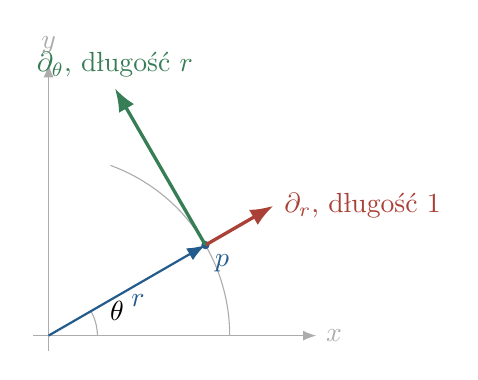
\begin{tikzpicture}[>=Latex,scale=1.0]
 \coordinate (O) at (0,0);
 \coordinate (P) at ({2.3*cos(30)},{2.3*sin(30)});
 \draw[->,gray!65] (-0.2,0)--(3.4,0) node[right] {$x$};
 \draw[->,gray!65] (0,-0.2)--(0,3.45) node[above] {$y$};
 \draw[gray!65] (2.3,0) arc[start angle=0,end angle=70,radius=2.3];
 \draw[gray!65] (0.62,0) arc[start angle=0,end angle=30,radius=0.62];
 \draw[->,thick,manifoldblue] (O)--(P)
    node[pos=0.57,below] {$r$};
 \fill[manifoldblue] (P) circle (1.5pt) node[below right] {$p$};
 \draw[->,very thick,manifoldred] (P)--++({cos(30)},{sin(30)})
    node[right] {$\partial_r$, długość $1$};
 \draw[->,very thick,manifoldgreen] (P)--++({-2.3*sin(30)},{2.3*cos(30)})
    node[above] {$\partial_\theta$, długość $r$};
 \node at (0.87,0.31) {$\theta$};
\end{tikzpicture}
\caption{Współrzędne biegunowe: wektor $\partial_r$ jest radialny,
a $\partial_\theta$ styczny do okręgu o promieniu $r$.
Współczynnik $r^2$ w metryce jest kwadratem długości drugiego wektora.}
\label{fig:tensor-biegunowe}
\end{figure}

Podobnie $\Lambda^k(T_pM)$ ma wymiar $\binom nk$.
W przypadku różniczki $\dd F_p\colon T_pM\to T_{F(p)}N$
między rozmaitościami tego samego wymiaru,
$\Lambda^n(\dd F_p)$ działa między ich jednowymiarowymi
potęgami zewnętrznymi. Jest niezerowe dokładnie wtedy,
gdy $\dd F_p$ jest izomorfizmem: wynika to z dowodu
Twierdzenia~\ref{thm:det-wlasnosci}, zastosowanego do baz
w dwóch różnych przestrzeniach. W mapach odpowiada temu
warunek niezerowego wyznacznika macierzy Jacobiego.
W odróżnieniu od endomorfizmu jednej przestrzeni, dla odwzorowania
$T_pM\to T_{F(p)}N$ nie otrzymujemy jednak kanonicznego skalara
„wyznacznik” bez wyboru baz lub elementów objętości w obu włóknach.
Kanoniczne jest odwzorowanie $\Lambda^n(\dd F_p)$ między
dwiema prostymi; jego macierz liczbową określają wybrane mapy.

\begin{uwaga}[Cztery sposoby widzenia tej samej konstrukcji]
Iloczyn tensorowy powstaje z dwuliniowości
(Definicja~\ref{def:tensor-universal}); algebra tensorowa
gromadzi wszystkie stopnie i mnoży przez konkatenację
(Definicja~\ref{def:algebra-tensorowa}). Symetryzator
$\operatorname{Sym}_k$ wybiera część niezmienniczą względem
permutacji, zaś $\operatorname{Alt}_k$ część zmieniającą znak.
Algebra zewnętrzna jest ilorazem, w którym kwadrat każdego
wektora znika (Definicja~\ref{def:algebra-zewnetrzna}).
Twierdzenie~\ref{thm:wedge-alt} mówi dokładnie, jak przejść
od tego ilorazu do tensorów antysymetrycznych.
\end{uwaga}

\section{Różniczkowanie pól tensorowych: pochodna Liego}
\label{sec:lie-tensory}

Pole tensorowe ma wartości w różnych przestrzeniach nad
różnymi punktami. Dlatego wyrażenie ,,odejmij $T_q-T_p$''
nie ma sensu, dopóki nie wskażemy sposobu przeniesienia
obu tensorów do jednego włókna. W Sekcji~\ref{sec:liego}
przepływ pola $X$ zrobił to dla pól wektorowych;
ta sama konstrukcja działa na każdym typie tensora.

Samo różniczkowanie współczynników w mapie nie rozwiązuje
problemu: ich pochodne zmieniają się przy zmianie współrzędnych.
Na przykład na $(0,\infty)$ wektor $Y=\partial_x$ ma w
mapie $x$ stały współczynnik $Y^x=1$, więc
$\partial_xY^x=0$. Po podstawieniu $y=x^2$ mamy
$Y=2\sqrt y\,\partial_y$ i
$\partial_yY^y=1/\sqrt y\ne0$.
Różnica pochodzi od zmiany samej bazy $\partial_y$.
Pochodna Liego uwzględnia również tę zmianę.

\begin{definicja}[Cofnięcie pola tensorowego]
\index{cofniecie pola tensorowego@Cofnięcie pola tensorowego}
\label{def:cofniecie-tensora}
Niech $F\colon U\to V$ będzie dyfeomorfizmem między
otwartymi podzbiorami $M$. Dla pola wektorowego $Y$ i
pola kowektorowego $\alpha$ na $V$ definiujemy w $p\in U$
\begin{align*}
 (F^*Y)_p&:=(\dd F_p)^{-1}Y_{F(p)}\in T_pM,\\
 (F^*\alpha)_p(v)&:=\alpha_{F(p)}(\dd F_pv),
 \qquad v\in T_pM.
\end{align*}
Dla funkcji kładziemy $F^*f=f\circ F$.
Na tensorach prostych cofamy każdy czynnik osobno,
np.\ $F^*(Y\otimes\alpha)=F^*Y\otimes F^*\alpha$,
i przedłużamy liniowo na sumy w każdym włóknie. Do gładkości
wystarczy lokalne rozwinięcie w bazie tensorowej; nie zakładamy
istnienia jednej globalnej bazy ani globalnego rozkładu na tensory proste.
Dostajemy pole
tego samego typu na $U$. W szczególności
$F^*(fT)=(f\circ F)F^*T$, a nie $fF^*T$.
Współczynniki są gładkie: różniczka i jej macierz odwrotna
zależą gładko od punktu, a działania tensorowe są wieloliniowe.
\end{definicja}

Przy cofaniu wektora używamy odwrotnej różniczki,
a przy cofaniu kowektora różniczki bez odwracania:
obie wartości muszą ostatecznie należeć do włókna nad $p$.
Wzór dla tensorów prostych jest dobrze określony na
iloczynach tensorowych, ponieważ każda z operacji na
czynnikach jest liniowa. W szczególności cofnięcie zachowuje
iloczyn tensorowy i kontrakcję. To drugie można sprawdzić
na jednej parze:
\[
 (F^*\alpha)_p\bigl((F^*Y)_p\bigr)
 =\alpha_{F(p)}\bigl(\dd F_p(\dd F_p)^{-1}Y_{F(p)}\bigr)
 =\alpha_{F(p)}(Y_{F(p)}).
\]
Obie strony są cofnięciem funkcji $p\mapsto\alpha_p(Y_p)$;
z liniowości wynikają analogiczne równości dla innych tensorów.

\begin{figure}[H]
\centering
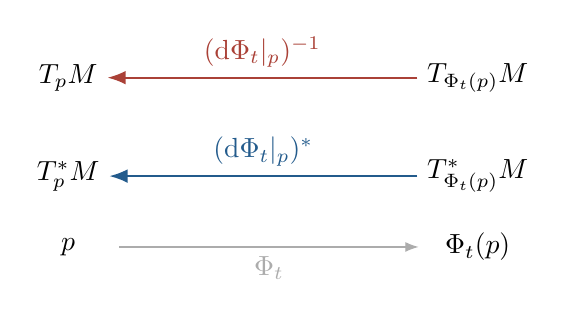
\begin{tikzpicture}[>=Latex]
 \node (Tp) at (0,2) {$T_pM$};
 \node (Tq) at (5.2,2) {$T_{\Phi_t(p)}M$};
 \node (Tps) at (0,0.75) {$T_p^*M$};
 \node (Tqs) at (5.2,0.75) {$T_{\Phi_t(p)}^*M$};
 \draw[->,thick,manifoldred] (Tq) --
    node[above] {$(\dd\Phi_t|_p)^{-1}$} (Tp);
 \draw[->,thick,manifoldblue] (Tqs) --
    node[above] {$(\dd\Phi_t|_p)^*$} (Tps);
 \node at (0,-0.15) {$p$};
 \node at (5.2,-0.15) {$\Phi_t(p)$};
 \draw[->,gray!65] (0.65,-0.15) --
    node[below] {$\Phi_t$} (4.45,-0.15);
\end{tikzpicture}
\caption{Cofnięcie przez przepływ przenosi wektor i kowektor
z włókien nad $\Phi_t(p)$ do włókien nad $p$.
Wektor przenosi odwrotna różniczka, a kowektor różniczka dualna.}
\label{fig:lie-tensor-transport}
\end{figure}

\begin{definicja}[Pochodna Liego dowolnego pola tensorowego]
\index{pochodna liego dowolnego pola tensorowego@Pochodna Liego dowolnego pola tensorowego}
\label{def:lie-tensor}
Niech $\Phi_t=\Phi_t^X$ oznacza lokalny przepływ pola $X$.
Dla pola tensorowego $T$ dowolnego typu kładziemy
\begin{equation}\label{eq:lie-tensor-def}
 (\Lie_XT)_p
 :=\left.\frac{\dd}{\dd t}\right|_{t=0}
 (\Phi_t^*T)_p.
\end{equation}
W otoczeniu każdego $p$ przepływ jest określony dla $t$
z pewnego przedziału wokół zera; dla takiego $t$
$\Phi_t$ jest dyfeomorfizmem między odpowiednimi otwartymi
podzbiorami $M$. Transport obrazuje
Rysunek~\ref{fig:lie-tensor-transport}.
Każdy tensor $(\Phi_t^*T)_p$ należy do tej samej
przestrzeni $T^r_s(T_pM)$, zatem pochodna jest
zwykłą pochodną krzywej w przestrzeni liniowej. Jest to gładkie
pole tensorowe: w każdej mapie współczynniki cofnięcia są gładkie
łącznie w $(t,p)$, więc ich pochodne po $t$ w zerze są gładkie w $p$.
\end{definicja}

W stopniu $(0,0)$ wzór~\eqref{eq:lie-tensor-def} daje
$\Lie_Xf=X(f)$, ponieważ $\Phi_t^*f=f\circ\Phi_t$.
Dla typu $(1,0)$ odzyskujemy dokładnie
$\Lie_XY=[X,Y]$ z Twierdzenia~\ref{thm:lie-nawias}.
Dowód tamtego twierdzenia wyjaśnia szczegółowo znak:
przenosimy $Y_{\Phi_t(p)}$ z powrotem różniczką
przepływu $\Phi_{-t}$.

\begin{twierdzenie}[Reguła Leibniza i zgodność z kontrakcją]
\label{thm:lie-tensor-reguly}
Dla pól tensorowych $S,T$, funkcji $f$, pola wektorowego
$Y$ i pola kowektorowego $\alpha$ mamy
\begin{align}
 \Lie_X(S\otimes T)
 &= (\Lie_XS)\otimes T+S\otimes(\Lie_XT),
 \label{eq:lie-tensor-leibniz}\\
 \Lie_X(fT)&=X(f)T+f\Lie_XT,
 \label{eq:lie-tensor-funkcja}\\
 (\Lie_X\alpha)(Y)
 &=X\bigl(\alpha(Y)\bigr)-\alpha([X,Y]),
 \label{eq:lie-kowektor}\\
 \Lie_X(C(S))&=C(\Lie_XS),
 \label{eq:lie-kontrakcja}
\end{align}
gdzie w ostatnim wzorze $C$ jest dowolną kontrakcją
jednego indeksu wektorowego z jednym kowektorowym.
\end{twierdzenie}
\begin{proof}
Ustalmy punkt $p$. Cofnięcie zachowuje iloczyn tensorowy:
$\Phi_t^*(S\otimes T)=\Phi_t^*S\otimes\Phi_t^*T$.
Obie krzywe tensorów po prawej stronie leżą w stałych
przestrzeniach nad $p$; różniczkując ich iloczyn
dwuliniowy w $t=0$ dostajemy
\eqref{eq:lie-tensor-leibniz}. Traktując $f$ jako tensor
typu $(0,0)$, otrzymujemy
\eqref{eq:lie-tensor-funkcja} z $\Lie_Xf=X(f)$.

Dla kowektora i wektora równanie o zachowaniu ewaluacji,
wykazane tuż przed definicją, przyjmuje postać
\[
 \Phi_t^*\bigl(\alpha(Y)\bigr)
 =(\Phi_t^*\alpha)(\Phi_t^*Y).
\]
Lewa strona po zróżniczkowaniu w zerze wynosi
$X(\alpha(Y))$. Prawa, przez zwykłą regułę
różniczkowania wartości kowektora na wektorze,
wynosi $(\Lie_X\alpha)(Y)+\alpha(\Lie_XY)$.
Z~$\Lie_XY=[X,Y]$ otrzymujemy
\eqref{eq:lie-kowektor}.

Wreszcie, cofnięcie i kontrakcja spełniają
$\Phi_t^*C(S)=C(\Phi_t^*S)$, co dla pojedynczej
pary sprawdziliśmy powyżej. Kontrakcja jest liniowym
odwzorowaniem między przestrzeniami tensorów w $p$, więc
można ją przenieść przez pochodną po $t$.
To daje~\eqref{eq:lie-kontrakcja}.
\end{proof}

\begin{twierdzenie}[Wzór we współrzędnych]
\label{thm:lie-tensor-wspolrzedne}
Niech $X=\sum_{a=1}^nX^a\partial_a$ i niech $T$ ma
współczynniki $T^I{}_J$ z~\eqref{eq:pole-tensorowe-lokalnie},
gdzie $I=(i_1,\ldots,i_r)$ i $J=(j_1,\ldots,j_s)$.
Symbol $I_{\mu\leftarrow a}$ oznacza zastąpienie w $I$
indeksu $i_\mu$ przez $a$, a $J_{\nu\leftarrow a}$
oznacza to samo w $J$. Wtedy
\begin{equation}\label{eq:lie-tensor-komponenty}
\begin{aligned}
 (\Lie_XT)^I{}_J
 &=\sum_{a=1}^nX^a\partial_a T^I{}_J
 -\sum_{\mu=1}^r\sum_{a=1}^n
   (\partial_aX^{i_\mu})T^{I_{\mu\leftarrow a}}{}_J\\
 &\quad+\sum_{\nu=1}^s\sum_{a=1}^n
   (\partial_{j_\nu}X^a)T^I{}_{J_{\nu\leftarrow a}}.
\end{aligned}
\end{equation}
Pierwszy wyraz różniczkuje funkcje współczynnikowe,
każdy indeks wektorowy wnosi wyraz z minusem,
a każdy indeks kowektorowy wyraz z plusem.
Na przykład dla pola operatorów $S\in\Gamma(T^1_1M)$
wzór ten ma łatwą do odczytania postać
\[
 (\Lie_XS)^i{}_j
 =\sum_a X^a\partial_aS^i{}_j
  -\sum_a S^a{}_j\partial_aX^i
  +\sum_a S^i{}_a\partial_jX^a.
\]
\end{twierdzenie}
\begin{proof}
Z~\eqref{eq:nawias-wspolrzedne}, zastosowanego do
$Y=\partial_i$, wynika
\[
 \Lie_X\partial_i=[X,\partial_i]
 =-\sum_a(\partial_iX^a)\partial_a,
\]
ponieważ współczynniki pola $\partial_i$ są stałe.
Z kolei $\dd x^j(\partial_i)=\delta_i^j$ jest funkcją
stałą. Wstawiając $Y=\partial_i$ i $\alpha=\dd x^j$
do~\eqref{eq:lie-kowektor}, dostajemy
\[
 (\Lie_X\dd x^j)(\partial_i)
 =X(\delta_i^j)-\dd x^j([X,\partial_i])
 =\partial_iX^j.
\]
Wektory $\partial_i$ tworzą bazę, zatem
$\Lie_X\dd x^j=\sum_i(\partial_iX^j)\dd x^i$.
Teraz rozwińmy $T$ według~\eqref{eq:pole-tensorowe-lokalnie}
i stosujmy~\eqref{eq:lie-tensor-leibniz} kolejno
do funkcji współczynnikowej oraz do każdego czynnika.
Różniczkowanie funkcji daje pierwszy wyraz
\eqref{eq:lie-tensor-komponenty}. Dla ustalonego miejsca
wektorowego $\mu$ współczynnik przy bazowym
$\partial_{i_\mu}$ po zróżniczkowaniu wcześniejszego
czynnika $\partial_a$ wynosi
$-\sum_a(\partial_aX^{i_\mu})T^{I_{\mu\leftarrow a}}{}_J$;
sumowanie po $\mu$ daje drugi wyraz wzoru.
Dla ustalonego miejsca kowektorowego $\nu$ wcześniejszy
czynnik $\dd x^a$ wnosi do współczynnika przy
$\dd x^{j_\nu}$ sumę
$\sum_a(\partial_{j_\nu}X^a)T^I{}_{J_{\nu\leftarrow a}}$;
po zsumowaniu po $\nu$ otrzymujemy trzeci wyraz.
Ponieważ tensory bazowe są liniowo niezależne,
ich współczynniki są dokładnie podanymi wyrażeniami.
\end{proof}

\begin{przyklad}[Sprawdzenie znaków na przepływie]
Na $\R^2$ weźmy $X=x\partial_x$. Jego przepływ to
$\Phi_t(x,y)=(e^tx,y)$, więc
\[
 \Phi_t^*\partial_x=e^{-t}\partial_x,
 \qquad \Phi_t^*\dd x=e^t\dd x.
\]
Po zróżniczkowaniu w zerze otrzymujemy
$\Lie_X\partial_x=-\partial_x=[X,\partial_x]$
oraz $\Lie_X\dd x=\dd x$. Pierwszy znak jest ujemny,
bo cofamy wektor różniczką odwrotnego przepływu;
drugi dodatni, bo kowektor działa na różniczce przepływu.
Wyniki są zgodne z tym, że $\dd x(\partial_x)=1$
pozostaje funkcją stałą: $1+(-1)=0$ w regule
Leibniza dla ewaluacji.
\end{przyklad}

\begin{przyklad}[Znoszenie się znaków w tensorze mieszanym]
Dla tego samego przepływu weźmy
$S=\partial_x\otimes\dd x$. Wówczas
\[
 \Phi_t^*S=(e^{-t}\partial_x)\otimes(e^t\dd x)=S,
 \qquad \Lie_XS=0.
\]
Formuła współrzędnych potwierdza to dla jedynego
niezerowego współczynnika $S^x{}_x=1$:
$X(S^x{}_x)-S^x{}_x\partial_xX^x+
S^x{}_x\partial_xX^x=0-1+1=0$.
Kontrakcja $C(S)=\dd x(\partial_x)=1$ również ma
pochodną Liego równą zeru, zgodnie z
\eqref{eq:lie-kontrakcja}.
\end{przyklad}

Jeżeli tensor metryczny ma postać
$g=\sum_{i,j}g_{ij}\dd x^i\otimes\dd x^j$, to
ogólny wzór~\eqref{eq:lie-tensor-komponenty} przyjmuje postać
\[
 (\Lie_Xg)_{ij}
 =\sum_a\bigl(X^a\partial_a g_{ij}
  +g_{aj}\partial_iX^a+g_{ia}\partial_jX^a\bigr).
\]
Ostatnie dwa wyrazy opisują zmianę dwóch argumentów
metryki pod przepływem.

\begin{przyklad}[Jak zmienia się tensor metryczny]
Dla $g=\dd x\otimes\dd x+\dd y\otimes\dd y$ i
$X=x\partial_x$ mamy
\[
 (\Phi_t^*g)_p(v,w)
 =g_{\Phi_t(p)}(\dd\Phi_t|_p v,\dd\Phi_t|_p w).
\]
Ponieważ $\dd\Phi_t$ mnoży składową $x$ wektora przez
$e^t$, otrzymujemy
\[
 \Phi_t^*g=e^{2t}\dd x\otimes\dd x
             +\dd y\otimes\dd y,\qquad
 \Lie_Xg=2\dd x\otimes\dd x.
\]
Przepływ rozciąga kierunek $x$; gdy tensor mierzy
iloczyny skalarne dwóch wektorów, pojawia się czynnik
$e^t$ dla każdego z dwóch kowektorowych miejsc.
\end{przyklad}

\begin{uwaga}[Jaką pochodną zdefiniowaliśmy?]
Pochodna Liego porównuje tensory za pomocą przepływu
\emph{konkretnego} pola $X$. Jej wzór wymaga tylko struktury
gładkiej i pola $X$. Jeśli chcielibyśmy porównywać tensory
wzdłuż dowolnej krzywej bez wskazanego przepływu,
potrzebowalibyśmy dodatkowej reguły przenoszenia między
przestrzeniami stycznymi, nazywanej \emph{koneksją} (połączeniem).
Na przykład $\Lie_{x\partial_x}\partial_x=-\partial_x$
chociaż współczynniki pola $\partial_x$ są stałe:
wynik uwzględnia ruch bazy pod przepływem.
\end{uwaga}

\par\smallskip
{\footnotesize\noindent\emph{Dalsza lektura:}
\href{https://math.stanford.edu/~conrad/diffgeomPage/handouts/tensor.pdf}
{B. Conrad, \emph{Tensor algebras, tensor pairings, and duality}},
notatki do Math 396, s. 1--13: własności uniwersalne i dualność;
\href{https://doi.org/10.1007/978-1-4419-9982-5}
{J. M. Lee, \emph{Introduction to Smooth Manifolds}, wyd. 2},
rozdziały 12 i 14: pola tensorowe, formy alternujące
i pochodne Liego.\par}
\clearpage

\chapter{Grassmanniany, algebra Clifforda i spinory}
\label{ch:grass-spin}

\providecommand{\atlasref}[2]{#2}

\index{grupa spin@Grupa Spin}

W Rozdziale~\ref{ch:algebra-tensorowa} skonstruowaliśmy iloczyn
zewnętrzny i wiązki tensorowe. Teraz zadamy trzy kolejne pytania:
jak opisać \emph{przestrzeń wszystkich podprzestrzeni} danego wymiaru,
jak zmienić algebrę zewnętrzną, aby uwzględniała iloczyn skalarny,
i dlaczego obrót o $2\pi$ może zmieniać znak spinora.
Odpowiedzi prowadzą kolejno do grassmannianów, algebr Clifforda
i grup Spin. Przykłady w wymiarach $2$ i $3$ pozwolą nam
sprawdzać każdą konwencję znaku na konkretnych macierzach.

\section{Grassmannian jako przestrzeń podprzestrzeni}
\label{sec:grass-atlas}

\noindent\emph{Powiązania tematyczne w Bibliotece matematycznej:} \atlasref{LA-29::thm:lin29-grass-atlas}{LA-29: atlas Grassmannianu}.


W trzech pierwszych sekcjach przez $\mathbb K$ oznaczamy
$\R$ albo $\C$.
Jeśli $0\leq k\leq n$, \emph{grassmannian}
$\operatorname{Gr}_k(\mathbb K^n)$ to zbiór wszystkich
$k$-wymiarowych podprzestrzeni liniowych $\mathbb K^n$.
Jego \emph{punktem} jest cała podprzestrzeń $L$,
a nie wektor w $L$. Na przykład
$\operatorname{Gr}_1(\R^n)=\mathbb{RP}^{n-1}$
z Przykładu~\ref{prz:RPn}, a
$\operatorname{Gr}_1(\C^n)=\mathbb{CP}^{n-1}$.
Dla $k=0$ i $k=n$ grassmannian jest jednym punktem.
Dla dowolnej $n$-wymiarowej przestrzeni $V$ nad $\mathbb K$
piszemy analogicznie $\operatorname{Gr}_k(V)$; wybór bazy
identyfikuje go z powyższym modelem, lecz konstrukcje nie zależą od tej bazy.

\begin{twierdzenie}[Mapy wykresowe grassmannianu]
\label{thm:grass-atlas}
Niech $\mathbb K^n=P\oplus Q$, gdzie $\dim_{\mathbb K}P=k$.
Zbiór
\[
 U_P=\{L\in\operatorname{Gr}_k(\mathbb K^n):
           \pi_P|_L:L\longrightarrow P\text{ jest izomorfizmem}\}
\]
można jednoznacznie opisać odwzorowaniami liniowymi
$A:P\to Q$: punktowi $A$ odpowiada jego
\emph{wykres} $\Gamma(A)=\{u+Au:u\in P\}$.
Mapy $\Gamma(A)\mapsto A$ tworzą gładki atlas
grassmannianu. Jego wymiar nad $\mathbb K$ wynosi
$k(n-k)$. W przypadku zespolonym atlas jest holomorficzny,
a rzeczywisty wymiar wynosi $2k(n-k)$.
Oznaczenie $U_P$ zależy również od wybranego dopełnienia $Q$;
pomijamy je w indeksie tylko dla skrócenia zapisu.
\end{twierdzenie}
\begin{proof}
Jeśli $L=\Gamma(A)$, to $\pi_P(u+Au)=u$, więc
$\pi_P|_L$ jest izomorfizmem. W drugą stronę, dla
$L\in U_P$ określmy
\[
 A_L:=\pi_Q|_L\circ(\pi_P|_L)^{-1}:P\longrightarrow Q.
\]
Każdy $v\in L$ ma postać $u+\pi_Qv=u+A_Lu$
dla $u=\pi_Pv$. Stąd $L=\Gamma(A_L)$; dowiedliśmy
zarówno istnienia, jak i jednoznaczności parametru.

Sprawdźmy przejścia między mapami, a nie tylko ich
liczbę. Niech $\mathbb K^n=P'\oplus Q'$ będzie drugim
rozkładem. Dla $A:P\to Q$ połóżmy
$T_A:P\to\mathbb K^n$, $T_A(u)=u+Au$.
Wykres $\Gamma(A)$ należy do $U_{P'}$ dokładnie wtedy,
gdy $D_A:=\pi_{P'}T_A:P\to P'$ jest odwracalny.
Po wybraniu baz $P,P'$ wyznacznik macierzy $D_A$ zależy
wielomianowo od współczynników $A$;
warunek $\det D_A\ne0$ jest więc otwarty. W nowej mapie
parametr ma postać
\begin{equation}\label{eq:grass-przejscie}
 A'=\pi_{Q'}T_A\circ(\pi_{P'}T_A)^{-1}:P'\longrightarrow Q'.
\end{equation}
Odwracanie macierzy jest gładkie na zbiorze macierzy
odwracalnych, a nad $\C$ jest tam także holomorficzne
(wzór przez dopełnienia algebraiczne i wyznacznik).
Każde $L$ leży w $U_L$, bo dla rozkładu
$\mathbb K^n=L\oplus Q$ otrzymujemy $A_L=0$.
Atlasy pokrywają zatem cały zbiór. Współczynniki
$A\in\operatorname{Hom}_{\mathbb K}(P,Q)$ tworzą
przestrzeń $\mathbb K^{(n-k)k}$, co daje wymiar.

Definiujemy topologię przez atlas: zbiór jest otwarty, gdy
jego obraz w każdej z map wykresowych jest otwarty.
Otwartość dziedzin przejść i ich ciągłość zapewniają, że
same $U_P$ są otwarte, a mapy są homeomorfizmami.
Uzasadnijmy również pozostałe własności topologiczne.
Wybierzmy standardowy iloczyn skalarny, a nad $\C$ hermitowski;
gwiazdka oznacza operator sprzężony. W tym kroku
ograniczmy się do rozkładów ortogonalnych $Q=P^\perp$;
takie mapy wciąż pokrywają cały grassmannian
(dla danego $L$ bierzemy $P=L$).
Wzór~\eqref{eq:grass-przejscie} zapewnia zgodność
z pozostałymi mapami. Każdemu $L$
przypiszmy macierz rzutowania ortogonalnego $\Pi_L$.
Jest ona wyznaczona jednoznacznie przez $L$, a jej
współczynniki w mapie wykresowej są gładkie:
\[
 \Pi_{\Gamma(A)}
  =T_A(T_A^*T_A)^{-1}T_A^*.
\]
Wyprowadźmy ten wzór z warunku prostopadłości.
Obraz $T_A$ to $\Gamma(A)$, więc rzut wektora $v$ ma postać
$T_Au$. Różnica $v-T_Au$ ma być prostopadła do wszystkich
$T_Aw$; równoważnie $T_A^*(v-T_Au)=0$.
Stąd $(T_A^*T_A)u=T_A^*v$ i otrzymujemy wypisany wzór.
Macierz $G_A:=T_A^*T_A=I+A^*A$ jest odwracalna, ponieważ
$\langle G_Au,u\rangle=\|u\|^2+\|Au\|^2>0$ dla $u\ne0$.
Odwrót na $U_P$ jest również ciągły w macierzach
rzutowania, ponieważ dla $L\in U_P$
\[
 A_L=\pi_Q\Pi_L|_P\,(\pi_P\Pi_L|_P)^{-1}.
\]
Istotnie, w rozkładzie $P\oplus Q$ mamy
$T_Au=(u,Au)$ i $T_A^*(u,0)=u$.
Zatem $\pi_P\Pi_L|_P=G_A^{-1}$ oraz
$\pi_Q\Pi_L|_P=AG_A^{-1}$, a złożenie w ostatnim wzorze
wynosi $(AG_A^{-1})(G_A^{-1})^{-1}=A$.
Ostatnia odwrotność istnieje, gdyż przy ortogonalnym
rzutowaniu $\pi_P$ odwzorowanie $\Pi_L|_P:P\to L$
jest sprzężeniem izomorfizmu
$\pi_P|_L:L\to P$. Nasza topologia zgadza się więc
z topologią podzbioru macierzy rzutowania: $U_P$ jest w tym
modelu zbiorem, gdzie $\pi_P\Pi_L|_P$ jest odwracalne,
a więc zbiorem otwartym. Oba podane wzory są ciągłe na tych mapach.
Zbiór $\Pi^*=\Pi$, $\Pi^2=\Pi$, $\operatorname{tr}\Pi=k$
jest domknięty i ograniczony w skończenie wymiarowej
przestrzeni macierzy, a więc zwarty. Istotnie, samosprzężone
idempotenty mają wartości własne $0,1$, więc norma operatorowa
jest co najwyżej $1$, a ślad jest rangą. Są zatem dokładnie
rzutami na $k$-płaszczyzny. Ten model jest także
Hausdorffa i ma przeliczalną bazę. Atlas definiuje
zatem rozmaitość w sensie Rozdziału~\ref{ch:rozmaitosci}.
\end{proof}

\begin{figure}[!htbp]
\centering
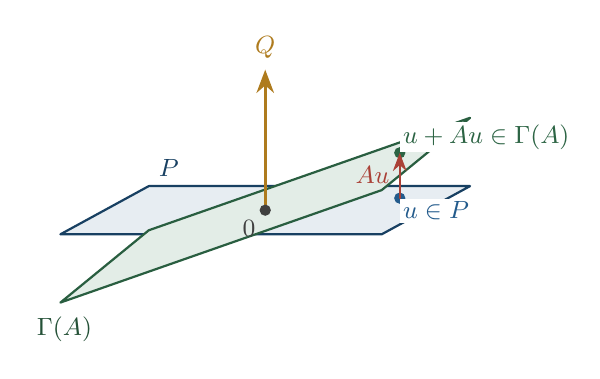
\begin{tikzpicture}[>=Stealth,line cap=round,line join=round,scale=1.02]
 \filldraw[fill=manifoldblue!11,draw=manifoldblue!70!black,thick]
 (-2.55,-.3)--(1.45,-.3)--(2.55,.3)--(-1.45,.3)--cycle;
 \filldraw[fill=manifoldgreen!14,draw=manifoldgreen!75!black,thick]
 (-2.55,-1.15)--(1.45,.25)--(2.55,1.15)--(-1.45,-.25)--cycle;
 \draw[->,manifoldgold!85!black,very thick] (0,0)--(0,1.75)
  node[above,font=\small] {$Q$};
 \fill[black!75] (0,0) circle (2pt) node[below left,font=\small] {$0$};
 \fill[manifoldblue] (1.675,.15) circle (2pt)
  node[below right,fill=white,inner sep=1pt,font=\small] {$u\in P$};
 \fill[manifoldgreen!80!black] (1.675,.715) circle (2pt)
  node[above right,fill=white,inner sep=1pt,font=\small] {$u+Au\in\Gamma(A)$};
 \draw[->,manifoldred,thick] (1.675,.15)--(1.675,.715)
  node[midway,left,font=\small] {$Au$};
 \node[manifoldblue!70!black,font=\small\bfseries] at (-1.2,.52) {$P$};
 \node[manifoldgreen!65!black,font=\small\bfseries] at (-2.5,-1.48) {$\Gamma(A)$};
\end{tikzpicture}
\caption{Mapa wykresowa grassmannianu. Przestrzeń $P$ jest
punktem odniesienia; pobliska płaszczyzna $\Gamma(A)$ powstaje,
gdy nad $u\in P$ odkładamy przemieszczenie $Au\in Q$.}
\label{fig:grass-wykres}
\end{figure}

\begin{przyklad}[Mała mapa, a nie cały grassmannian]
\label{prz:grass-rp1-mapy}
Na $\operatorname{Gr}_1(\R^2)=\mathbb{RP}^1$ ustalmy
$P=\R e_1$ i $Q=\R e_2$. Prosta
$L_a=\operatorname{span}(e_1+ae_2)$ ma współrzędną
$a\in\R$. Brakuje dokładnie jednej prostej, $\R e_2$:
rzutowanie na $P$ jest na niej zerowe. Zatem mapa
wykresowa jest lokalna, podobnie jak mapa stereograficzna
nie pokrywa całej sfery.

W drugiej mapie, z $P'=\R e_2$ i $Q'=\R e_1$,
zapisujemy $L=\operatorname{span}(be_1+e_2)$.
Na części wspólnej obu map $a\ne0$ i
\[
 e_1+ae_2=a\bigl(a^{-1}e_1+e_2\bigr),
 \qquad b=\frac1a.
\]
To najprostszy przypadek wzoru~\eqref{eq:grass-przejscie}:
druga mapa dopisuje prostą $\R e_2$, której nie ma
w pierwszej; jej współrzędna $b=0$ odpowiada
,,$a=\infty$'' w potocznym opisie.
\end{przyklad}

\section{Przestrzeń styczna i wiązka tautologiczna}
\label{sec:grass-styczna}

Wektor styczny do grassmannianu opisuje \emph{pierwszy
rząd zmiany podprzestrzeni}. Wektory należące już do
danej podprzestrzeni nie zmieniają jej położenia:
istotna jest część wychodząca poza nią.
Z każdej z $k$ niezależnych osi podprzestrzeni możemy
wyjść w $n-k$ niezależnych kierunkach poprzecznych;
stąd intuicyjnie bierze się wymiar $k(n-k)$.

\begin{twierdzenie}[Styczne jako odwzorowania do ilorazu]
\label{thm:grass-styczna}
Dla $L\in\operatorname{Gr}_k(V)$ istnieje kanoniczny
izomorfizm
\begin{equation}\label{eq:grass-styczna}
 T_L\operatorname{Gr}_k(V)
  \cong\operatorname{Hom}_{\mathbb K}(L,V/L).
\end{equation}
Nad $\C$ prawa strona jest zespoloną przestrzenią
styczną; jej podłożem rzeczywistym jest rzeczywista
przestrzeń styczna.
\end{twierdzenie}
\begin{proof}
Niech $L(t)$ będzie gładką krzywą podprzestrzeni,
$L(0)=L$. Dla $v\in L$ wybierzmy gładką krzywą
$v(t)\in L(t)$ z $v(0)=v$. Definiujemy
$D_{L'(0)}(v):=[v'(0)]\in V/L$, gdzie nawias oznacza
klasę modulo $L$. Pokażmy niezależność od wyboru
$v(t)$. Różnica dwóch takich krzywych $w(t)\in L(t)$
ma $w(0)=0$. W gładkiej lokalnej bazie $s_i(t)$
zapisuje się $w(t)=\sum_i a_i(t)s_i(t)$ z
$a_i(0)=0$, zatem
$w'(0)=\sum_i a_i'(0)s_i(0)\in L$. Klasa
$[v'(0)]$ nie zmienia się. Zmiana parametryzacji
krzywej nie jest jedyną możliwą zmianą przedstawiciela wektora
stycznego; niezależność od dowolnej krzywej o tym samym wektorze
stycznym sprawdzimy teraz w mapie.

Ustalmy teraz uzupełnienie $V=L\oplus Q$.
W mapie z Twierdzenia~\ref{thm:grass-atlas} mamy
$L(t)=\Gamma(A(t))$ i $A(0)=0$.
Wybieramy $v(t)=v+A(t)v$. Wtedy
\[
 D_{L'(0)}(v)=[A'(0)v]\in V/L.
\]
Tak samo $s_i(t)=e_i+A(t)e_i$ dla bazy $(e_i)$ przestrzeni $L$
daje gładką bazę używaną powyżej. Wzór zależy tylko od $A'(0)$,
czyli współrzędnych wektora stycznego, a nie od dalszego przebiegu krzywej.
Jeśli $D_{L'(0)}=0$, to $A'(0)v\in Q\cap L=0$ dla każdego $v$,
więc $A'(0)=0$ i wektor styczny jest zerowy. To dowodzi iniektywności.
Utożsamienie $Q\cong V/L$ pokazuje, że
$D_{L'(0)}$ jest liniowe w $v$. Każdy
$D\in\operatorname{Hom}(L,V/L)$ można otrzymać:
wybierzmy odpowiadające mu odwzorowanie $A:L\to Q$
i krzywą $L(t)=\Gamma(tA)$. Jej pochodna daje
właśnie $D$. Konstrukcja rozpoczęła się od
krzywej i klas modulo $L$, więc otrzymany
izomorfizm nie zależy od wybranego $Q$.
\end{proof}

\begin{przyklad}[Wektor styczny do przestrzeni prostych]
Niech $L_0=\R e_1\in\operatorname{Gr}_1(\R^2)$ i
$L(t)=\R(e_1+t e_2)$. W mapie z
Przykładu~\ref{prz:grass-rp1-mapy}
współrzędna krzywej to $a(t)=t$, więc jej prędkość
wynosi $a'(0)=1$. Dla wektora $v=s e_1\in L_0$
wybieramy $v(t)=s(e_1+t e_2)\in L(t)$; z definicji
\[
 D_{L'(0)}(s e_1)=[s e_2]\in\R^2/L_0.
\]
Zatem pojedyncza liczba $a'(0)$ jest macierzą
odwzorowania $L_0\to\R^2/L_0$ w bazach
$e_1$ i $[e_2]$. Krzywa
$\widetilde L(t)=\R(\cos t\,e_1+\sin t\,e_2)$
daje ten sam wektor styczny, bo jej współrzędna
$\tan t$ także ma pochodną $1$ w zerze.
\end{przyklad}

\begin{definicja}[Wiązka tautologiczna]
\index{wiazka tautologiczna@Wiązka tautologiczna}
\label{def:grass-taut}
Nad $\operatorname{Gr}_k(V)$ określamy
\emph{wiązkę tautologiczną}
\[
 \gamma^k
 :=\{(L,v)\in\operatorname{Gr}_k(V)\times V:v\in L\}
 \longrightarrow\operatorname{Gr}_k(V),\qquad (L,v)\mapsto L.
\]
Jej włókno w punkcie $L$ jest dosłownie podprzestrzenią
$L\subseteq V$.
\end{definicja}

\begin{stwierdzenie}[Lokalność i wiązka ilorazowa]
\label{prop:grass-wiazki}
Wiązka $\gamma^k$ ma rząd $k$. Jest podwiązką
wiązki trywialnej $\operatorname{Gr}_k(V)\times V$.
Istnieje też wiązka ilorazowa $\mathcal Q$ z
włóknem $\mathcal Q_L=V/L$, rzędu $n-k$,
oraz kanoniczny dokładny ciąg wiązek
\begin{equation}\label{eq:grass-ciag}
 0\longrightarrow\gamma^k
 \longrightarrow\operatorname{Gr}_k(V)\times V
 \longrightarrow\mathcal Q\longrightarrow0.
\end{equation}
Po wybraniu iloczynu skalarnego otrzymujemy
$\mathcal Q\cong(\gamma^k)^\perp$.
\end{stwierdzenie}
\begin{proof}
Na $U_P$ każdy element $L=\Gamma(A)$ zawiera
dokładnie jeden wektor $u+Au$ dla danego $u\in P$.
Odwzorowanie $(L,u)\mapsto(L,u+Au)$ jest zatem lokalną
trywializacją $U_P\times P\cong\gamma^k|_{U_P}$;
jej odwrotność to $(L,v)\mapsto(L,\pi_Pv)$.
Oba odwzorowania są gładkie, a na włóknach liniowe.
W tym samym rozkładzie $V=P\oplus Q$ klasa
$[w]\in V/\Gamma(A)$ ma jednoznacznego
reprezentanta w $Q$: od $w$ odejmujemy
$u+Au\in\Gamma(A)$, gdzie $u=\pi_Pw$.
Stąd lokalnie $\mathcal Q|_{U_P}\cong U_P\times Q$.
Na każdym włóknie inkluzja $L\hookrightarrow V$
jest iniekcją, a naturalne odwzorowanie $V\to V/L$ jest
surjekcją z jądrem $L$, co wyjaśnia \emph{dokładność}
ciągu~\eqref{eq:grass-ciag}. Iloczyn skalarny
identyfikuje klasę $[v]$ z $(\id-\Pi_L)v\in L^\perp$.
Rzut zależy gładko od $L$, więc jest to izomorfizm wiązek,
a nie tylko rodzina izomorfizmów włókien.
\end{proof}

\begin{uwaga}[Jeszcze jedno zastosowanie Rozdziału 3]
Twierdzenie~\ref{thm:grass-styczna} i
izomorfizm tensorowy~\ref{thm:tensor-hom} dają
\[
 T\operatorname{Gr}_k(V)\cong
       (\gamma^k)^*\otimes\mathcal Q.
\]
Włókno po prawej stronie w $L$ to
$L^*\otimes(V/L)\cong\operatorname{Hom}(L,V/L)$.
Kolejność czynników jest tu ważna: źródłem odwzorowania
jest $L$, a jego wartości należą do $V/L$.
Zgodność tych izomorfizmów z gładkością również widać w mapie:
przy $L=\Gamma(A)$ przyrost $\dot A$ wysyła $u+Au$ na
klasę $\dot A u$. W trywializacji ilorazu
$[w]\mapsto\pi_Qw-A\pi_Pw$ ma on po prostu macierz $\dot A$.
Zatem izomorfizmy włókien sklejają się w gładki izomorfizm wiązek.
\end{uwaga}

\begin{przyklad}[Proste w płaszczyźnie i wstęga Möbiusa]
Na $\operatorname{Gr}_1(\R^2)\cong\mathbb{RP}^1\cong S^1$
wiązka $\gamma^1$ jest wstęgą Möbiusa z
Przykładu~\ref{prz:mobius}. Istotnie,
$L(t)=\R(\cos t,\sin t)$, $0\leq t\leq\pi$,
opisuje pełne okrążenie bazy: $L(0)=L(\pi)$.
Wybrany lokalnie wektor jednostkowy
$(\cos t,\sin t)\in L(t)$ wraca jako jego
przeciwieństwo. To właśnie sklejanie włókna
ze zmianą znaku.
W dwóch mapach z Przykładu~\ref{prz:grass-rp1-mapy} tę zmianę
widać również w funkcji przejścia: jeśli
$\lambda(e_1+ae_2)=\mu(be_1+e_2)$ oraz $b=1/a$,
to porównanie współczynników daje $\mu=a\lambda$.
Na dwóch składowych części wspólnej ($a>0$ i $a<0$)
funkcja przejścia ma przeciwne znaki. Właśnie tego
nie da się usunąć przez jeden globalny wybór
niezerowego wektora w każdym włóknie: zmiana
lokalnej ramki (Definicja~\ref{def:ramka-lokalna})
przez funkcję nigdzie niezerową
ma na każdej spójnej mapie stały znak.
\end{przyklad}

\section{Orientacja, współrzędne Plückera i odwzorowanie Gaussa}
\label{sec:grass-plucker}

\begin{definicja}[Grassmannian zorientowany]
\index{grassmannian zorientowany@Grassmannian zorientowany}
Punkt $\operatorname{Gr}^+_k(\R^n)$ to para $(L,o)$:
$k$-płaszczyzna $L$ wraz z wyborem jej orientacji $o$.
Zapomnienie orientacji daje dwukrotne nakrycie
$\operatorname{Gr}^+_k(\R^n)\to\operatorname{Gr}_k(\R^n)$
dla $0<k<n$: nad każdą płaszczyzną są dokładnie
dwie możliwe orientacje. W mapie wykresowej
orientację przenosimy z $P$ na $\Gamma(A)$ przez
$u\mapsto u+Au$, więc lokalnie nakrycie jest
sumą dwóch kopii tej samej mapy.
\end{definicja}

\begin{przyklad}[Płaszczyzny w $\R^3$]
Płaszczyźnie $L\in\operatorname{Gr}_2(\R^3)$
odpowiada jej nieukierunkowana prosta normalna
$L^\perp$, a zatem
$\operatorname{Gr}_2(\R^3)\cong\mathbb{RP}^2$.
Gdy $L$ ma orientację, wybierzmy dodatnią bazę
ortonormalną $(u,v)$ i połóżmy $n=u\times v$.
Inna dodatnia baza różni się obrotem w $L$,
więc daje ten sam $n$. W drugą stronę $n\in S^2$
wyznacza $L=n^\perp$ i orientację, dla której
$(u,v,n)$ jest dodatnią bazą $\R^3$. Otrzymujemy
\[
 \operatorname{Gr}^+_2(\R^3)\cong S^2,\qquad
 \operatorname{Gr}_2(\R^3)\cong S^2/(n\sim -n).
\]
Zmiana orientacji płaszczyzny zamienia $n$ z $-n$.
Dla ustalenia gładkości zauważmy, że normalna z lokalnej dodatniej
ramki ortonormalnej jest gładka. W drugą stronę rzut
na $n^\perp$ ma macierz $I-nn^T$, gładką w $n$;
lokalny wybór orientacji jest stały na każdym z dwóch płatów.
Są to więc dyfeomorfizmy, nie tylko bijekcje zbiorów.
\end{przyklad}

\begin{figure}[!htbp]
\centering
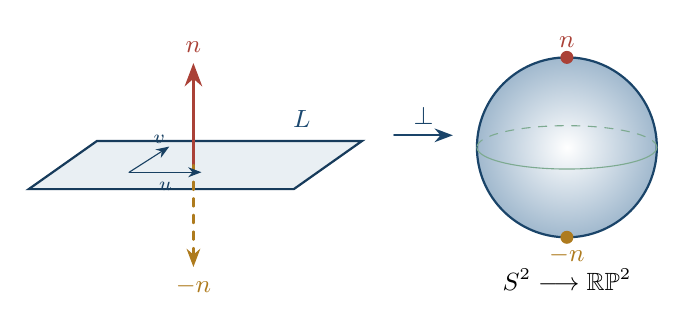
\begin{tikzpicture}[>=Stealth,line cap=round,scale=1.02]
 \filldraw[fill=manifoldblue!10,draw=manifoldblue!65!black,thick]
 (-4.6,-.52)--(-1.3,-.52)--(-.45,.08)--(-3.75,.08)--cycle;
 \draw[->,very thick,manifoldred] (-2.55,-.22)--(-2.55,1.05)
   node[above,font=\small] {$n$};
 \draw[->,thick,manifoldgold!85!black,dashed]
   (-2.55,-.22)--(-2.55,-1.49)
   node[below,font=\small] {$-n$};
 \node[font=\small,manifoldblue!80!black] at (-1.2,.35) {$L$};
 \draw[->,manifoldblue!70!black] (-3.35,-.31)--(-2.45,-.31)
   node[midway,below,font=\scriptsize] {$u$};
 \draw[->,manifoldblue!70!black] (-3.35,-.31)--(-2.85,.01)
   node[near end,above,font=\scriptsize] {$v$};
 \shade[inner color=white,outer color=manifoldblue!43] (2.1,0) circle (1.12);
 \draw[manifoldblue!75!black,thick] (2.1,0) circle (1.12);
 \draw[manifoldgreen!65,thin] (.98,0) arc[start angle=180,end angle=360,x radius=1.12,y radius=.27];
 \draw[manifoldgreen!65,thin,dashed] (3.22,0)
   arc[start angle=0,end angle=180,x radius=1.12,y radius=.27];
 \fill[manifoldred] (2.1,1.12) circle (2.3pt)
   node[above,font=\small] {$n$};
 \fill[manifoldgold!85!black] (2.1,-1.12) circle (2.3pt)
   node[below,font=\small] {$-n$};
 \draw[->,manifoldblue!75!black,thick] (-.05,.15)--(.68,.15)
   node[midway,above,font=\small] {$\perp$};
 \node[font=\small] at (2.1,-1.65) {$S^2\longrightarrow\mathbb{RP}^2$};
\end{tikzpicture}
\caption{Orientacja płaszczyzny w $\R^3$ wybiera jedną z
dwóch jednostkowych normalnych. Zapomnienie orientacji
utożsamia punkty antypodyczne $n$ i $-n$ na sferze.}
\label{fig:grass-normalne}
\end{figure}

\begin{stwierdzenie}[Bazy ortonormalne i przestrzeń ilorazowa]
\label{prop:grass-stiefel}
Niech $V_k(\R^n)$ będzie zbiorem uporządkowanych
ortonormalnych $k$-ramek $(v_1,\ldots,v_k)$.
Odwzorowanie $(v_i)\mapsto\operatorname{span}(v_i)$ ma
włókna izomorficzne z $\mathrm O(k)$.
Ponadto, jako gładkie przestrzenie,
\[
 \operatorname{Gr}_k(\R^n)
   \cong\mathrm O(n)/(\mathrm O(k)\times\mathrm O(n-k)),
\quad
 \operatorname{Gr}_k(\C^n)
   \cong\mathrm U(n)/(\mathrm U(k)\times\mathrm U(n-k)).
\]
\end{stwierdzenie}
\begin{proof}
Dwie ramki wyznaczają tę samą $k$-płaszczyznę wtedy
i tylko wtedy, gdy zmiana bazy między nimi należy do
$\mathrm O(k)$. Wykonując ortonormalizację Grama--Schmidta
na wektorach $u_i+Au_i$ z mapy wykresowej, dostajemy
gładki lokalny wybór ramki; włókna są więc lokalnie
kopiami $\mathrm O(k)$. Grupa $\mathrm O(n)$ działa
tranzytywnie na płaszczyznach: wybieramy bazy ortonormalne
dwóch płaszczyzn, uzupełniamy je do baz $\R^n$ i bierzemy
odwzorowanie przenoszące pierwszą pełną bazę na drugą.
Element zachowujący standardowe $\R^k$ zachowuje też
jego dopełnienie prostopadłe, czyli ma postać blokową
$\mathrm{diag}(B,C)$ z $B\in\mathrm O(k)$,
$C\in\mathrm O(n-k)$. To daje pierwszy iloraz.
Wyjaśnijmy gładką strukturę ilorazu. W rozkładzie ortogonalnym
$P\oplus Q$ uzupełniamy ramkę wykresu przez ramkę
$\Gamma(-A^*)\subset Q\oplus P$ jego dopełnienia prostopadłego:
jej wektory mają postać $-A^*w+w$, $w\in Q$.
Ortonormalizacja obu ramek daje macierz $s(A)\in\mathrm O(n)$
zależną gładko od $A$. Każda macierz ortogonalna nad tą mapą
ma jednoznaczną postać $s(A)\operatorname{diag}(B,C)$.
Parametr $A$ odzyskujemy z obrazu pierwszych $k$ kolumn,
a bloki $B,C$ z iloczynu $s(A)^{-1}O$. Daje to lokalny
produkt i jego gładką odwrotność; po podzieleniu przez bloki
pozostaje dokładnie mapa wykresowa grassmannianu.
Argument dla $\C$ jest taki sam, z bazami unitarnymi,
sprzężeniem hermitowskim i grupą $\mathrm U(n)$.
\end{proof}

Iloczyn zewnętrzny z Sekcji~\ref{sec:algebra-zewnetrzna}
pozwala zapisać $k$-płaszczyznę jednym wielowektorem,
określonym z dokładnością do niezerowego skalara.
Po wyborze bazy $(e_i)$ przestrzeni $V$ oraz zapisaniu
$v_j=\sum_i v_{ij}e_i$ współczynnik
$p_I$ przy $e_{i_1}\wedge\cdots\wedge e_{i_k}$
ma postać minora
$\det(v_{i_a j})_{1\leq a,j\leq k}$, gdzie
$I=(i_1<\cdots<i_k)$; jest to
wzór~\eqref{eq:wedge-rozwiniecie-minory} z Rozdziału~3.
Liczby $p_I$ nazywamy \emph{współrzędnymi Plückera}.
Zmiana bazy $L$ mnoży je wszystkie przez tę samą
niezerową liczbę $\det C$, więc geometryczną informację
niesie ich klasa rzutowa $[p_I]$.

\begin{twierdzenie}[Zanurzenie Plückera]
\label{thm:grass-plucker}
Jeśli $(v_1,\ldots,v_k)$ jest bazą $L$, to wzór
\begin{equation}\label{eq:plucker}
 \mathrm{Pl}(L):=[v_1\wedge\cdots\wedge v_k]
 \in\mathbb P(\Lambda^k V)
\end{equation}
określa gładkie zanurzenie
$\operatorname{Gr}_k(V)\hookrightarrow\mathbb P(\Lambda^k V)$.
Nawias $[\xi]$ oznacza prostą $\mathbb K\xi$,
$\xi\ne0$. Obraz składa się dokładnie z klas
niezerowych \emph{wielowektorów prostych}.
\end{twierdzenie}
\begin{proof}
Zmiana bazy $(v_i)$ macierzą $C$ mnoży iloczyn
zewnętrzny przez $\det C\ne0$ na mocy
Twierdzenia~\ref{thm:det-wlasnosci}, więc klasa
rzutowa jest dobrze określona. Jeżeli
$\xi=v_1\wedge\cdots\wedge v_k\ne0$, to
\[
 L=\{w\in V:w\wedge\xi=0\}.
\]
Wektory z $L$ dają zero przez powtórzenie czynnika.
Jeśli $w\notin L$, rodzina $(v_1,\ldots,v_k,w)$
jest liniowo niezależna; po uzupełnieniu do bazy
Twierdzenie~\ref{thm:wedge-baza} mówi, że jej
iloczyn zewnętrzny jest niezerowy. Zatem
$\mathrm{Pl}(L)$ wyznacza $L$ jednoznacznie.

Pokażmy, skąd bierze się gładki odwrotny wzór na obrazie.
W mapie $V=P\oplus Q$ wybierzmy bazy
$e_1,\ldots,e_k$ przestrzeni $P$ oraz
$e_{k+1},\ldots,e_n$ przestrzeni $Q$ i zapiszmy
$Ae_j=\sum_{a=1}^{n-k}a_{aj}e_{k+a}$.
W wielowektorze
$\xi_A=(e_1+Ae_1)\wedge\cdots\wedge(e_k+Ae_k)$
współczynnik $p_{1\cdots k}$ wynosi $1$.
Współczynnik przy
$e_1\wedge\cdots\wedge\widehat{e_j}\wedge\cdots
\wedge e_k\wedge e_{k+a}$ wynosi
$(-1)^{k-j}a_{aj}$: przesuwamy $e_{k+a}$
przez $k-j$ późniejszych czynników.
Z ilorazów tych współczynników przez $p_{1\cdots k}$
odzyskujemy wszystkie $a_{aj}$.
Jeśli dla dowolnego indeksu $I$ mamy $p_I\ne0$,
to rzut bazy $L$ na płaszczyznę
$P=\operatorname{span}\{e_i:i\in I\}$ ma wyznacznik $p_I$.
Jest więc izomorfizmem $L\to P$ i możemy stosować
analogiczny wzór w mapie $U_P$, dzieląc przez $p_I$.
Odwzorowanie~\eqref{eq:plucker} jest więc gładkie.
Wzory odzyskujące $a_{aj}$ są określone na całym otwartym
zbiorze przestrzeni rzutowej $p_{1\cdots k}\ne0$, nie tylko
na obrazie. Ich złożenie z $\mathrm{Pl}$ jest odwzorowaniem identycznościowym
w parametrach $A$; różniczkowanie daje lewą odwrotność różniczki
$\mathrm{Pl}$, która jest zatem injektywna.
Otrzymaliśmy immersję. Grupy $\mathrm O(n)$ i $\mathrm U(n)$
są zwarte jako domknięte i ograniczone zbiory macierzy.
Ich ilorazy z~\ref{prop:grass-stiefel}, a więc oba
grassmanniany, są zwarte jako ciągłe obrazy grup zwartych.
Ponieważ przestrzeń rzutowa jest Hausdorffa,
ciągła iniekcja ze zwartego grassmannianu jest
homeomorfizmem na obraz. To daje zanurzenie i domkniętość obrazu.
\end{proof}

\begin{przyklad}[Relacja Plückera dla $\operatorname{Gr}_2(\R^4)$]
Zapiszmy $\xi=\sum_{1\leq i<j\leq4}p_{ij}e_i\wedge e_j$.
Rozwińmy $\xi\wedge\xi$. Składnik z powtórzonym
indeksem znika, więc zostają tylko pary $12|34$, $13|24$
i $14|23$ oraz te same pary w odwrotnej kolejności.
Pierwsza para jest już uporządkowana; w drugiej
przestawienie $1,3,2,4$ do $1,2,3,4$ wymaga jednej
transpozycji, a w trzeciej przestawienie $1,4,2,3$
wymaga dwóch. Znaki wynoszą zatem kolejno $+,-,+$.
Każda para występuje dwukrotnie z tym samym znakiem,
bo zamiana dwóch bloków stopnia $2$ daje $(-1)^4=1$.
Otrzymujemy
\begin{equation}\label{eq:plucker-24}
 \xi\wedge\xi=
 2(p_{12}p_{34}-p_{13}p_{24}+p_{14}p_{23})
   e_1\wedge e_2\wedge e_3\wedge e_4.
\end{equation}
Jeżeli $\xi=u\wedge v$, to $\xi\wedge\xi=0$,
więc współczynniki spełniają relację w nawiasie.
Odwrotnie, dla $\xi\ne0$ z taką relacją możemy
przestawić współrzędne tak, by $p_{12}\ne0$.
Po podzieleniu przez $p_{12}$ ustawiamy w wykresie
$e_1+ae_3+ce_4$, $e_2+be_3+de_4$ liczby
$b=p_{13}/p_{12}$, $d=p_{14}/p_{12}$,
$a=-p_{23}/p_{12}$, $c=-p_{24}/p_{12}$.
Pięć współczynników się zgadza z definicji,
a szósty jest równy $ad-bc=p_{34}/p_{12}$
właśnie dzięki relacji: po podstawieniu
$ad-bc=(p_{13}p_{24}-p_{14}p_{23})/p_{12}^2$,
a relacja daje w liczniku $p_{12}p_{34}$.
To dowodzi również
wystarczalności.

Policzmy wszystkie współrzędne dla
$L=\operatorname{span}(e_1+2e_3,e_2+e_4)$:
\[
 (e_1+2e_3)\wedge(e_2+e_4)
  =e_1\wedge e_2+e_1\wedge e_4
   -2e_2\wedge e_3+2e_3\wedge e_4.
\]
Mamy więc $(p_{12},p_{13},p_{14},p_{23},p_{24},p_{34})
=(1,0,1,-2,0,2)$ i relację $1\cdot2+1\cdot(-2)=0$.
Z kolei współrzędne wykresu odzyskujemy jako
$(a,b,c,d)=(2,0,0,1)$, zgodnie z wyjściową bazą.
W tym przypadku $\dim\operatorname{Gr}_2(\R^4)=4$,
podczas gdy $\mathbb P(\Lambda^2\R^4)$ ma wymiar $5$:
jedna relacja $p_{12}p_{34}-p_{13}p_{24}+p_{14}p_{23}=0$
opisuje więc cały obraz Plückera jako kwadrykę rzutową.
Dla kontrastu
$e_1\wedge e_2+e_3\wedge e_4$ ma
$p_{12}p_{34}=1$ i pozostałe wyrazy zerowe,
więc nie jest wielowektorem prostym, zgodnie
z wcześniejszym Przykładem w
Sekcji~\ref{sec:baza-zewnetrzna}.
\end{przyklad}

\begin{twierdzenie}[Odwzorowanie Gaussa i wiązka styczna]
\label{thm:grass-gauss}
Niech $M^m\subset\R^N$ będzie gładką podrozmaitością.
Przypisanie
$G(p)=T_pM\in\operatorname{Gr}_m(\R^N)$
jest gładkim \emph{odwzorowaniem Gaussa}. Wiązki
$TM$ i normalna $\nu M$ są odpowiednio
cofnięciami $G^*\gamma^m$ i $G^*\mathcal Q$
z~\eqref{eq:grass-ciag}.
\end{twierdzenie}
\begin{proof}
W mapie podrozmaitości zapisujemy jej parametryzację
$F:U\subset\R^m\to\R^N$. Wektory
$\partial_iF(x)$ tworzą gładką bazę $T_{F(x)}M$.
W pobliżu ustalonego punktu pewien minor $m\times m$
macierzy $\dd F$ pozostaje niezerowy. W odpowiadającym
mu rozkładzie $\R^N=P\oplus Q$ przestrzeń
$T_{F(x)}M$ jest wykresem macierzy
$A(x)=D_QF(x)(D_PF(x))^{-1}$,
gładkiej w $x$. Stąd $G$ jest gładka.
Włókno $(G^*\gamma^m)_p$ to z definicji
$\gamma^m_{G(p)}=T_pM$; lokalne ramki po obu
stronach są tymi samymi $\partial_iF$.
Włókno $(G^*\mathcal Q)_p$ to
$\R^N/T_pM$, czyli $\nu_pM$ z
Przykładu o wiązce normalnej w Sekcji o podrozmaitościach
Rozdziału~\ref{ch:rozmaitosci}.
Zgodność lokalnych trywializacji daje oba
izomorfizmy wiązek.
\end{proof}

\begin{przyklad}[Odwzorowanie Gaussa paraboli]
Dla paraboli $M=\{(t,t^2):t\in\R\}\subset\R^2$
weźmy parametryzację $F(t)=(t,t^2)$. Wówczas
\[
 F'(t)=(1,2t),\qquad
 G(F(t))=\R(1,2t),\qquad a(t)=2t
\]
w mapie $\operatorname{Gr}_1(\R^2)$ z
Przykładu~\ref{prz:grass-rp1-mapy}.
W punkcie $p=F(0)$ różniczka odwzorowania Gaussa
odpowiada, według~\eqref{eq:grass-styczna},
odwzorowaniu $T_pM\to\R^2/T_pM$ danemu przez
$e_1\mapsto2[e_2]$. Liczba $2$ mierzy tutaj
pierwszy rząd zmiany kierunku stycznej, podczas gdy
położenie punktu $F(t)$ nie występuje we współrzędnej $a(t)$.
Po utożsamieniu ilorazu z prostopadłą prostą
jednostkowa normalna ma postać
$(-2t,1)/\sqrt{1+4t^2}$.
\end{przyklad}

\begin{uwaga}[Dlaczego wiązka tautologiczna jest uniwersalna?]
Na zwartej rozmaitości każdą gładką rzeczywistą wiązkę $E$
rzędu $k$ można umieścić w trywialnej wiązce
$M\times\R^N$ dla pewnego $N$.
Oto konstrukcja. Wybieramy skończone pokrycie
trywializujące $U_i$, jego mniejsze podpokrycie
oraz funkcje gładkie $\beta_i$ o nośnikach w $U_i$,
takie że dla każdego $p$ co najmniej jedna
$\beta_i(p)$ jest niezerowa. Jeśli $[v]_i\in\R^k$
oznacza współrzędne $v\in E_p$ na $U_i$,
definiujemy różnowartościowe odwzorowanie liniowe w $v$
\[
 j_p(v)=\bigl(\beta_1(p)[v]_1,\ldots,
                  \beta_r(p)[v]_r\bigr)\in\R^{kr},
\]
przyjmując wartość $0$ dla bloku poza $U_i$.
Podparcie $\beta_i$ wewnątrz $U_i$ zapewnia
gładkość po przedłużeniu zerem; co najmniej
jeden niezerowy blok zapewnia iniektywność $j_p$.
Obrazy $j_p(E_p)$ zmieniają się gładko, ponieważ
lokalnie tworzą kolumny macierzy gładkiej i
stałego rzędu $k$, a więc definiują odwzorowanie
$f:M\to\operatorname{Gr}_k(\R^{kr})$.
Wprost z definicji włókien mamy
$E\cong f^*\gamma^k$. Ta konkretna konstrukcja
wyjaśnia użyteczność grassmannianów dla topologii
wiązek; nie potrzebuje jeszcze teorii klas
charakterystycznych.
W przypadku wiązki zespolonej ten sam rachunek
prowadzimy w $\C^{kr}$ i otrzymujemy mapę do
$\operatorname{Gr}_k(\C^{kr})$.
\end{uwaga}

\section{Algebra Clifforda: iloczyn i dowód wymiaru}
\label{sec:clifford}

\noindent\emph{Powiązania tematyczne w Bibliotece matematycznej:} \atlasref{LA-30::thm:lin30-cliff-baza}{LA-30: baza algebry Clifforda}.


Od tego miejsca $V$ jest rzeczywistą przestrzenią
euklidesową wymiaru $n$ z iloczynem skalarnym
$\langle\cdot,\cdot\rangle$ i normą
$\|v\|^2=\langle v,v\rangle$. Algebra zewnętrzna
pamięta zorientowane pola: $v\wedge v=0$.
Algebra Clifforda pamięta ponadto \emph{długość}:
kwadrat wektora jest skalarem $-\|v\|^2$.
Przyjmujemy konsekwentnie ten znak minus;
w literaturze spotyka się również konwencję przeciwną.

\begin{definicja}[Algebra Clifforda]
\index{algebra clifforda@Algebra Clifforda}
\label{def:clifford}
Niech $I_q$ będzie ideałem obustronnym algebry
tensorowej $T(V)$ z Definicji~\ref{def:algebra-tensorowa},
generowanym przez
$v\otimes v+\|v\|^2\,1$ dla wszystkich $v\in V$.
\emph{Algebra Clifforda} to
\[
 \operatorname{Cl}(V):=T(V)/I_q.
\]
Obraz $v\in V$ oznaczamy nadal $v$,
a mnożenie w ilorazie zapisujemy bez symbolu $\otimes$.
Z definicji $v^2=-\|v\|^2\,1$.
\end{definicja}

Po usunięciu z relacji składnika $\|v\|^2\,1$
otrzymujemy algebrę zewnętrzną
(Definicja~\ref{def:algebra-zewnetrzna}).
Tak więc obie algebry startują z tej samej algebry
tensorowej; zmieniamy tylko relację, przez którą
dzielimy. W algebrze Clifforda nie można zachować
zwykłego stopnia tensorowego: relacja utożsamia
wyraz stopnia $2$ ze skalarem stopnia $0$.
Pozostaje rozróżnienie stopnia \emph{parzystego}
i \emph{nieparzystego}, bo oba wyrazy relacji
mają tę samą parzystość.
Oznaczamy odpowiadające podprzestrzenie przez
$\operatorname{Cl}^0(V)$ i $\operatorname{Cl}^1(V)$.
Jest to suma prosta: ideał $I_q$ rozkłada się na części
parzystą i nieparzystą, ponieważ jego generatory są parzyste,
a każdy mnożnik po lewej i prawej można rozdzielić
według parzystości. Iloraz zachowuje więc ten rozkład.
Iloczyn słów o parzystościach $i,j\in\{0,1\}$
ma parzystość $i+j$ modulo $2$; jest to
$\Z/2\Z$-stopniowanie algebry Clifforda.

\begin{twierdzenie}[Relacja Clifforda i własność uniwersalna]
\label{thm:cliff-relacje}
Dla $v,w\in V$ w $\operatorname{Cl}(V)$ zachodzi
\begin{equation}\label{eq:cliff-relacja}
 vw+wv=-2\langle v,w\rangle\,1.
\end{equation}
Jeżeli $\mathcal A$ jest łączną algebrą rzeczywistą
z jedynką, a $f:V\to\mathcal A$ jest liniowa i spełnia
$f(v)^2=-\|v\|^2 1_{\mathcal A}$ dla każdego $v$,
to istnieje dokładnie jeden homomorfizm algebr
$\widehat f:\operatorname{Cl}(V)\to\mathcal A$
przedłużający $f$.
\end{twierdzenie}
\begin{proof}
Rozwijając $(v+w)^2$ na dwa sposoby, otrzymujemy
\[
 v^2+vw+wv+w^2=-\|v+w\|^2\,1
  =-(\|v\|^2+\|w\|^2+2\langle v,w\rangle)\,1.
\]
Po odjęciu $v^2=-\|v\|^2 1$ i
$w^2=-\|w\|^2 1$ zostaje~\eqref{eq:cliff-relacja}.
Z Twierdzenia~\ref{thm:algebra-tensorowa-universal}
odwzorowanie $f$ przedłuża się jednoznacznie do homomorfizmu
$F:T(V)\to\mathcal A$. Dla każdego generatora ideału
$I_q$ mamy
$F(v\otimes v+\|v\|^2 1)
 =f(v)^2+\|v\|^2 1_{\mathcal A}=0$.
Jądro homomorfizmu jest ideałem, więc zawiera $I_q$.
Wobec tego wzór $\widehat f([t])=F(t)$
nie zależy od przedstawiciela $t\in T(V)$
i wyznacza żądany homomorfizm na ilorazie.
Jednoznaczność wynika stąd, że $V$ i jedynka
generują $\operatorname{Cl}(V)$.
\end{proof}

Przy bazie ortonormalnej $(e_1,\ldots,e_n)$
relacja~\eqref{eq:cliff-relacja} mówi
\begin{equation}\label{eq:cliff-orto}
 e_i^2=-1,\qquad e_ie_j=-e_je_i\quad(i\ne j).
\end{equation}
Stąd każdy iloczyn generatorów można uporządkować
rosnąco, redukując powtórzone indeksy.
Trudniejszą częścią jest wykazanie, że tak otrzymane
wyrazy nie mają dodatkowych relacji.

\begin{twierdzenie}[Baza algebry Clifforda]
\label{thm:cliff-baza}
Dla bazy ortonormalnej $e_1,\ldots,e_n$ elementy
\[
 1,\qquad e_{i_1}\cdots e_{i_r}
 \quad(1\leq i_1<\cdots<i_r\leq n,\ 1\leq r\leq n)
\]
stanowią bazę $\operatorname{Cl}(V)$. Zatem
$\dim_\R\operatorname{Cl}(V)=2^n$.
Dla $n\geq1$ części parzysta i nieparzysta mają
po $2^{n-1}$ wymiarów.
\end{twierdzenie}
\begin{proof}
\emph{Rozpinanie.} Obrazy słów $v_1\cdots v_r$
rozpinają iloraz $T(V)/I_q$. Po rozwinięciu każdego
$v_j$ w bazie wystarczą słowa z liter $e_i$.
Równości~\eqref{eq:cliff-orto} pozwalają zamienić
każde dwie sąsiednie różne litery (ze zmianą znaku)
i usunąć parę równych liter ($e_i^2=-1$).
Powtarzając te operacje, dostajemy kombinację
iloczynów o rosnących, różnych indeksach.

\emph{Niezależność.} Skorzystamy z algebry zewnętrznej
$\Lambda(V)$ z Rozdziału~\ref{ch:algebra-tensorowa}.
Na niej określmy dwie operacje:
\[
 \varepsilon(v)\omega:=v\wedge\omega,\qquad
 \iota_v(w_1\wedge\cdots\wedge w_r)
 :=\sum_{j=1}^r(-1)^{j-1}
   \langle v,w_j\rangle\,
   w_1\wedge\cdots\wedge\widehat{w_j}
       \wedge\cdots\wedge w_r .
\]
Kreska nad $w_j$ oznacza pominięcie tego czynnika;
przyjmujemy $\iota_v(1)=0$.
Wzór na $\iota_v$ jest wieloliniowy i alternujący
w $w_j$: przy zamianie dwóch sąsiednich argumentów składniki
pomijające inny argument zmieniają znak przez antysymetrię iloczynu
zewnętrznego, a dwa pozostałe zamieniają się miejscami z przeciwnymi
znakami. Zatem własność uniwersalna
z Twierdzenia~\ref{thm:wedge-multilinear}
zapewnia, że operator jest dobrze określony.
Bezpośrednio z tego wzoru otrzymujemy
\[
 \iota_v(w\wedge\omega)
  =\langle v,w\rangle\omega-w\wedge\iota_v\omega.
\]
Pierwszy składnik powstaje przy usunięciu pierwszego
czynnika; pozostałe mają o jeden minus więcej niż
w $\iota_v\omega$. Usunięcie dwóch czynników
w dwóch przeciwnych kolejnościach daje składniki
o przeciwnych znakach: dla pozycji $p<q$ ich znaki to
$(-1)^{p-1}(-1)^{q-2}$ oraz
$(-1)^{q-1}(-1)^{p-1}$. Po ich dodaniu
otrzymujemy zero, zatem $\iota_v^2=0$.
Również $\varepsilon(v)^2=0$, bo $v\wedge v=0$.
Jeżeli $c(v):=\varepsilon(v)-\iota_v$, to
\[
 c(v)^2
 =-\bigl(\varepsilon(v)\iota_v
          +\iota_v\varepsilon(v)\bigr)
 =-\|v\|^2\id_{\Lambda(V)}.
\]
Własność uniwersalna z poprzedniego twierdzenia
daje więc reprezentację
$c:\operatorname{Cl}(V)\to\operatorname{End}_\R(\Lambda V)$.
Przyłóżmy ją do $1\in\Lambda^0V$.
Dla różnych ortonormalnych $e_{i_j}$ wszystkie
kontrakcje pojawiające się podczas kolejnego
działania znikają: nowy $e_{i_j}$ jest prostopadły
do wcześniej utworzonych czynników. Stąd
\[
 c(e_{i_1}\cdots e_{i_r})\,1
    =e_{i_1}\wedge\cdots\wedge e_{i_r},\qquad
 c(1)\,1=1.
\]
Prawa strona przebiega bazę $\Lambda(V)$ z
Twierdzenia~\ref{thm:wedge-baza}. Jeśli kombinacja
uporządkowanych słów znikałaby w algebrze Clifforda,
jej działanie na $1$ dawałoby zerową kombinację
\emph{różnych} wektorów tej bazy. Wszystkie
współczynniki muszą więc być zerowe.
Słów o $r$ indeksach jest $\binom nr$;
sumując po $r$ otrzymujemy $2^n$.
Wreszcie bijekcja $I\mapsto I\triangle\{1\}$
zamienia podzbiory parzystej i nieparzystej
liczności, co dowodzi równości ich liczby.
\end{proof}

Na przykład w $\operatorname{Cl}(\R^2)$ redukcja słowa
$e_2e_1e_2=-e_1e_2^2=e_1$ łączy zamianę sąsiednich
generatorów z relacją $e_2^2=-1$. Dzięki dowodowi
niezależności wiemy, że taka redukcja nie ukrywa
żadnych dodatkowych relacji między słowami uporządkowanymi.

\begin{uwaga}[Podobne przestrzenie, różne mnożenia]
\label{rem:cliff-zewnetrzna}
Istnieje kanoniczny izomorfizm \emph{przestrzeni liniowych}
$\Lambda V\cong\operatorname{Cl}(V)$: wysyła
$v_1\wedge\cdots\wedge v_r$ na antysymetryzację
$\frac1{r!}\sum_{\sigma\in S_r}\operatorname{sgn}(\sigma)
 v_{\sigma(1)}\cdots v_{\sigma(r)}$.
Jest dobrze określony, bo wyrażenie jest alternujące;
na bazowych wektorach ortonormalnych daje
$e_{i_1}\cdots e_{i_r}$, więc poprzednie twierdzenie
zapewnia odwracalność. Nie jest to jednak izomorfizm
algebr: w $\Lambda V$ mamy $v\wedge v=0$,
a w $\operatorname{Cl}(V)$ mamy
$v^2=-\|v\|^2$. To wyjaśnia, dlaczego obie
przestrzenie mają wymiar $2^n$, choć kodują
inne mnożenia.
\end{uwaga}

\begin{przyklad}[Wymiary $0$, $1$ i $2$]
Dla $V=0$ otrzymujemy $\operatorname{Cl}(0)=\R$.
W wymiarze $1$, przy $e_1^2=-1$, każdy element
ma postać $a+be_1$ i mnoży się jak liczba
$a+bi\in\C$. Stąd $\operatorname{Cl}(\R)\cong\C$
\emph{jako algebra rzeczywista}.
W wymiarze $2$ baza $(1,e_1,e_2,e_1e_2)$
spełnia dokładnie relacje kwaternionów:
$e_1\leftrightarrow i$, $e_2\leftrightarrow j$,
$e_1e_2\leftrightarrow k$, zatem
$\operatorname{Cl}(\R^2)\cong\mathbb H$.
Sprawdźmy brakujący kwadrat i znaki:
$(e_1e_2)^2=-e_1^2e_2^2=-1$,
$e_2e_1=-e_1e_2$,
$e_2(e_1e_2)=-e_1e_2^2=e_1$ oraz
$(e_1e_2)e_1=-e_1^2e_2=e_2$.
Relacje $i^2=j^2=-1$ i $ij=-ji$ dają homomorfizm
wysyłający $e_1,e_2$ na $i,j$.
Obrazy czterech wektorów bazy to $1,i,j,k$, czyli baza
$\mathbb H$, więc ten homomorfizm jest izomorfizmem.
Na przykład $(e_1+2e_2)^2=-5$, podczas gdy
$(e_1+2e_2)\wedge(e_1+2e_2)=0$
w algebrze zewnętrznej. Porównujemy więc kwadraty tego samego wektora.
\end{przyklad}

\begin{stwierdzenie}[Iloczyn wektorów: skalar i dwuwektor]
\label{prop:cliff-wedge}
Przez powyższy izomorfizm przestrzeni liniowych
iloczyn Clifforda dwóch wektorów rozkłada się na
\begin{equation}\label{eq:cliff-rozdzial}
 vw=-\langle v,w\rangle
       +\tfrac12(vw-wv)
 \quad\longleftrightarrow\quad
 -\langle v,w\rangle+v\wedge w.
\end{equation}
\end{stwierdzenie}
\begin{proof}
Suma $vw+wv$ jest równa
$-2\langle v,w\rangle$ z~\eqref{eq:cliff-relacja}.
Dodając połowę tej sumy do połowy różnicy,
odzyskujemy $vw$. Antysymetryzacja
$v\wedge w\mapsto\tfrac12(vw-wv)$
jest przypadkiem stopnia $2$ opisanym w
poprzedniej uwadze.
\end{proof}

Przykładowo, dla $v=e_1+2e_2$ oraz $w=2e_1+e_2$
mamy $\langle v,w\rangle=4$ i
$v\wedge w=(1\cdot1-2\cdot2)e_1\wedge e_2
=-3e_1\wedge e_2$. W algebrze Clifforda dostajemy
więc $vw=-4-3e_1e_2$; część skalarna mierzy
iloczyn skalarny, a część stopnia $2$ mierzy
zorientowane pole równoległoboku.

\begin{figure}[!htbp]
\centering
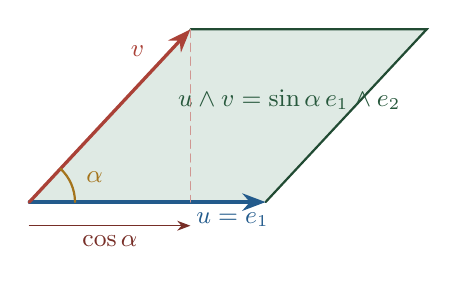
\begin{tikzpicture}[>=Stealth,line cap=round,scale=1.0]
 \coordinate (O) at (0,0);
 \coordinate (U) at (3.0,0);
 \coordinate (W) at ({3*cos(47)},{3*sin(47)});
 \coordinate (UW) at ({3+3*cos(47)},{3*sin(47)});
 \fill[manifoldgreen!16] (O)--(U)--(UW)--(W)--cycle;
 \draw[manifoldgreen!60!black,thick] (U)--(UW)--(W);
 \draw[->,manifoldblue,very thick] (O)--(U)
  node[pos=.86,below,font=\small] {$u=e_1$};
 \draw[->,manifoldred,very thick] (O)--(W)
  node[pos=.78,above left,font=\small] {$v$};
 \draw[densely dashed,manifoldred!55] (W)--({3*cos(47)},0);
 \draw[->,manifoldred!70!black] (0,-.3)--({3*cos(47)},-.3)
  node[midway,below,font=\small] {$\cos\alpha$};
 \draw[manifoldgold!80!black,thick] (.58,0)
  arc[start angle=0,end angle=47,radius=.58];
 \node[manifoldgold!80!black,font=\small] at (.83,.32) {$\alpha$};
 \node[manifoldgreen!70!black,font=\small] at (3.3,1.3)
  {$u\wedge v=\sin\alpha\,e_1\wedge e_2$};
\end{tikzpicture}
\caption{Dla jednostkowych $u=e_1$ i
$v=\cos\alpha\,e_1+\sin\alpha\,e_2$ iloczyn Clifforda
$uv=-\cos\alpha+\sin\alpha\,e_1e_2$ łączy
ujemny iloczyn skalarny ze zorientowanym polem.}
\label{fig:cliff-iloczyn}
\end{figure}

\section{Od odbić do grupy Spin}
\label{sec:spin-grupa}

Ustalmy najpierw dwie operacje na algebrze Clifforda.
Zmiana każdego $v$ na $-v$ zachowuje relacje definiujące,
więc daje automorfizm $\alpha$, z $\alpha^2=\id$.
Jego przestrzenie własne dla $+1$ i $-1$ są rozpięte
odpowiednio przez słowa parzyste i nieparzyste; dowód bazy
pokazuje, że ich suma jest prosta.
Drugą operacją jest \emph{rewersja}, oznaczana tyldą:
\[
 \widetilde{v_1\cdots v_r}=v_r\cdots v_1,\qquad
 \widetilde 1=1,
\]
przedłużona liniowo. Jest dobrze określona na ilorazie:
odwracanie słów w $T(V)$ ustala każdy generator
$v\otimes v+\|v\|^2 1$, a element $a(v\otimes v+\|v\|^2 1)b$
wysyła na $\widetilde b(v\otimes v+\|v\|^2 1)\widetilde a$,
nadal należący do ideału. Zatem
$\widetilde{st}=\widetilde t\,\widetilde s$ i
$\widetilde{\widetilde s}=s$, niezależnie od zapisu $s$ jako sumy słów.

Odbicie względem hiperpłaszczyzny prostopadłej
do jednostkowego $u\in V$ ma wzór
\begin{equation}\label{eq:spin-odbicie}
 r_u(v)=v-2\langle u,v\rangle u.
\end{equation}
Rozkład $v=\langle u,v\rangle u+w$, $w\perp u$,
pokazuje, że $r_u$ odwraca składową równoległą do $u$
i zostawia składową $w$. Jego wyznacznik jest równy $-1$.
Relacja Clifforda daje zaskakujący opis tego odbicia:
ponieważ $u^2=-1$, mamy $u^{-1}=-u$ i
\[
 -uvu^{-1}=uvu
 =-vu^2-2\langle u,v\rangle u
 =v-2\langle u,v\rangle u
 =r_u(v).
\]
W środkowej równości użyliśmy
$uv=-vu-2\langle u,v\rangle$. Znak minus przed
sprzężeniem jest niezbędny, aby obrazem było odbicie
w hiperpłaszczyźnie $u^\perp$ w każdym wymiarze.
Na przykład w $\R^3$ dla $u=e_1$ zwykłe sprzężenie
$v\mapsto uvu^{-1}$ ma w bazie standardowej macierz
$\operatorname{diag}(1,-1,-1)$, natomiast skręcone sprzężenie
$v\mapsto-uvu^{-1}$ ma macierz $\operatorname{diag}(-1,1,1)$.

\begin{definicja}[Grupa Pin]
\label{def:pin-grupa}
\index{grupa pin@Grupa Pin}
Dla euklidesowej przestrzeni $V$ grupą $\operatorname{Pin}(V)$
nazywamy podgrupę odwracalnych elementów $\operatorname{Cl}(V)$
złożoną ze wszystkich skończonych iloczynów wektorów
jednostkowych; dopuszczamy pusty iloczyn $1$.
W odróżnieniu od grupy Spin dopuszczamy także nieparzystą
liczbę czynników. Dla $s\in\operatorname{Pin}(V)$ określamy
\[
 \rho_{\mathrm{Pin}}(s)(v):=\alpha(s)v s^{-1},
 \qquad v\in V,
\]
gdzie $\alpha$ zmienia znak każdego wektora, jak wyżej.
\end{definicja}

Wzór jest skręconym sprzężeniem: dla jednostkowego $u$
daje $\rho_{\mathrm{Pin}}(u)(v)=-uvu^{-1}=r_u(v)$.
Zatem pojedynczy wektor reprezentuje odbicie, a jego parzysty
iloczyn reprezentuje obrót. Na przykład w $\R^2$ element
$e_1\in\operatorname{Pin}(2)$ daje odbicie w prostej
$e_1^\perp$: wysyła $e_1$ na $-e_1$, a $e_2$ pozostawia
bez zmiany. Z kolei $e_1e_2$ daje złożenie odbić
$r_{e_1}r_{e_2}=-\id_{\R^2}$, czyli obrót o pół obiegu.
Przy przyjętej relacji $u^2=-\|u\|^2$ grupa ta bywa
oznaczana $\operatorname{Pin}^{-}(n)$; znak rozróżnia dwie
konwencje algebry Clifforda.

\begin{definicja}[Grupa Spin]
\index{grupa spin@Grupa Spin}
\label{def:spin-grupa}
Niech $n=\dim V\geq2$. \emph{Grupą spinową}
$\operatorname{Spin}(V)$ nazywamy podgrupę
odwracalnych elementów $\operatorname{Cl}(V)$,
składającą się z iloczynów \emph{parzystej}
liczby wektorów jednostkowych:
\[
 \operatorname{Spin}(V)
 :=\{u_1\cdots u_{2r}:\|u_j\|=1,\ r\geq0\}.
\]
Pusty iloczyn to $1$. Skrót
$\operatorname{Spin}(n)$ oznacza
$\operatorname{Spin}(\R^n)$ ze standardową metryką.
Dla $s\in\operatorname{Spin}(V)$ określamy
$\rho(s)v:=svs^{-1}$.
Topologię na grupie bierzemy z jej inkluzji do skończenie
wymiarowej przestrzeni $\operatorname{Cl}(V)$. Gładką strukturę
zgodną z tą inkluzją uzasadnimy w dowodzie nakrycia.
\end{definicja}

Zbiór w definicji jest grupą: iloczyn dwóch słów
parzystych jest parzysty, a odwrotność słowa
$u_1\cdots u_{2r}$ to
$(-u_{2r})\cdots(-u_1)$, ponownie słowo parzyste
złożone z wektorów jednostkowych.
Każdy jego czynnik ma dobrze określoną odwrotność.

\begin{twierdzenie}[Dwukrotne nakrycie grupy obrotów]
\label{thm:spin-nakrycie}
Przypisanie $\rho$ jest surjektywnym homomorfizmem
\[
 \rho:\operatorname{Spin}(n)\longrightarrow\mathrm{SO}(n),
 \qquad\ker\rho=\{1,-1\}.
\]
Jest gładkim dwukrotnym nakryciem: każdy obrót
ma dokładnie dwa podniesienia $s$ i $-s$.
\end{twierdzenie}
\begin{proof}
\emph{Dlaczego obrazem jest obrót?}
Dla słowa $s=u_1\cdots u_{2r}$ zastosujmy
wzór na odbicie do kolejnych czynników.
W odwzorowaniu $v\mapsto-u v u^{-1}$ pojawia się
jedno odbicie $r_u$; przy parzystej liczbie
czynników wszystkie minusy się znoszą i
\[
 \rho(s)=r_{u_1}\circ\cdots\circ r_{u_{2r}}.
\]
To złożenie zachowuje iloczyn skalarny i ma
wyznacznik $(-1)^{2r}=1$. Ponieważ
$\rho(st)(v)=s(tvt^{-1})s^{-1}$,
$\rho$ jest homomorfizmem do $\mathrm{SO}(n)$.

\emph{Dlaczego jest surjektywna?}
Pokażmy elementarnie, że każdą izometrię liniową
można zapisać jako iloczyn odbić. Weźmy bazę
ortonormalną $e_1,\ldots,e_n$ i $A\in\mathrm O(n)$.
Jeśli $Ae_1\ne e_1$, to dla
$u=(Ae_1-e_1)/\|Ae_1-e_1\|$ rachunek z
\eqref{eq:spin-odbicie} daje $r_u(Ae_1)=e_1$:
licznik iloczynu
$\langle Ae_1-e_1,Ae_1\rangle$ to
$1-\langle Ae_1,e_1\rangle$, a kwadrat
mianownika to $2(1-\langle Ae_1,e_1\rangle)$.
Jeśli $Ae_1=e_1$, pomijamy ten krok.
Nowa izometria zachowuje $e_1$, więc działa
na $e_1^\perp$. Powtarzamy argument dla $e_2$
w tym dopełnieniu, potem dla $e_3$, itd.
Po skończenie wielu krokach otrzymujemy
identyczność. Zapisujemy więc $A$ jako
iloczyn odbić. Ponieważ $\det A=1$, liczba
użytych odbić musi być parzysta; odpowiadający
im iloczyn jednostkowych $u_j$ jest szukanym
elementem $\operatorname{Spin}(n)$.

\emph{Dlaczego jądro ma tylko dwa elementy?}
Niech $s$ działa trywialnie na $V$. Wtedy
$se_j=e_js$ dla każdego wektora bazy ortonormalnej.
Rozwińmy $s$ w bazie z
Twierdzenia~\ref{thm:cliff-baza}, używając tylko
słów parzystej długości:
$s=\sum_{|I|\ {\rm parzyste}}a_I e_I$.
Dla parzystego niepustego $I$ i $j\in I$
relacja~\eqref{eq:cliff-orto} daje
$e_je_Ie_j^{-1}=-e_I$; gdy $j\notin I$,
otrzymujemy $+e_I$.
Rzeczywiście, jeśli $j\notin I$, przenosimy $e_j$
przez $|I|$ różnych generatorów i dostajemy znak
$(-1)^{|I|}=1$. Jeśli $j\in I$, mija on tylko
$|I|-1$ innych generatorów, co daje znak $-1$;
czynnik $e_je_j^{-1}$ następnie się skraca. Równość
$e_jse_j^{-1}=s$ dla \emph{wszystkich} $j$
wymusza więc $a_I=0$ dla każdego niepustego $I$.
Zatem $s=a\,1$. Aby ustalić $a$, odwróćmy
porządek wektorów w słowie:
$\widetilde s=u_{2r}\cdots u_1$.
Wtedy $s\widetilde s=(-1)^{2r}=1$,
bo wektory są jednostkowe i $u_i^2=-1$.
Dla skalarnego $s=a$ również $\widetilde s=a$,
stąd $a^2=1$. Oba znaki występują,
gdyż $-1=e_1e_1\in\operatorname{Spin}(n)$.

\emph{Dlaczego rzeczywiście jest to nakrycie?}
Grupa $\mathrm O(n)$ ma strukturę gładkiej podrozmaitości
przestrzeni macierzy, skonstruowaną w przykładzie o grupie
ortogonalnej w Rozdziale~\ref{ch:rozmaitosci}.
Warunek $\det A=1$ wycina w niej otwartą i domkniętą
podrozmaitość $\mathrm{SO}(n)$.
Pokażmy, że w pobliżu identyczności obroty mają
gładko wybrane podniesienie. Dla bliskich
jednostkowych $a,b$ połóżmy
\[
 R(a,b):=-\frac{a+b}{\|a+b\|}\,a
       =\frac{1-ba}{\|a+b\|}\in\operatorname{Spin}(n).
\]
Jest to iloczyn dwóch jednostkowych wektorów,
zależy gładko od $(a,b)$, spełnia $R(a,a)=1$
i przenosi $a$ na $b$: pierwsze odbicie w
hiperpłaszczyźnie do $a$ wysyła $a$ na $-a$,
drugie, o normalnej $(a+b)/\|a+b\|$, wysyła
$-a$ na $b$.
W tym ostatnim kroku $u=(a+b)/\|a+b\|$ i wzór na odbicie dają
\[
 r_u(-a)
 =-a+\frac{2(1+\langle a,b\rangle)}{\|a+b\|^2}(a+b)
 =-a+(a+b)=b,
\]
ponieważ $\|a+b\|^2=2(1+\langle a,b\rangle)>0$.
Jeśli $A$ jest bliski identyczności,
stosujemy taki rotor, aby skorygować $Ae_1$ do
$e_1$. Otrzymany obrót zachowuje $e_1$.
W $e_1^\perp$ korygujemy następnie obraz
$e_2$, potem $e_3$, kończąc na $e_{n-1}$;
ostatni wektor jest ustalony dzięki wyznacznikowi
$1$. Każdy rotor zależy gładko od $A$
w niewielkim otoczeniu identyczności.
Odwrotność ich iloczynu daje gładką lokalną
sekcję $\sigma$ odwzorowania $\rho$.
Przy innym obrocie przenosimy to otoczenie
przez ustalony element z jego przeciwobrazu.
Wybierzmy otoczenie $U$ identyczności w $\mathrm{SO}(n)$
tak małe, aby $\sigma(A)$ było określone i współczynnik
przy $1$ w jego rozwinięciu w bazie Clifforda był większy
niż $1/2$ dla każdego $A\in U$; jest to możliwe, bo
$\sigma(\id)=1$. Obliczone jądro daje dokładnie
\[
 \rho^{-1}(U)=\sigma(U)\sqcup(-\sigma(U)).
\]
Pierwszy zbiór jest przecięciem $\rho^{-1}(U)$
z otwartym warunkiem dodatniości współczynnika skalarnego,
drugi odpowiada warunkowi ujemności tego współczynnika.
Oba są więc otwarte w $\operatorname{Spin}(n)$, a $\rho$
odwzorowuje każdy z nich homeomorficznie na $U$:
odwrotnościami są ciągłe odwzorowania $\sigma$ i $-\sigma$.
Mnożenie przez ustalone podniesienie przenosi tę konstrukcję
nad otoczenie dowolnego obrotu. Otrzymaliśmy zatem
dwukrotne nakrycie.
W ten sposób otrzymujemy także atlas gładki: na każdym płacie
używamy współrzędnych z $\mathrm{SO}(n)$ przeniesionych przez $\rho$.
Jest on zgodny z inkluzją do algebry Clifforda. Istotnie,
$\sigma$ jest gładka jako odwzorowanie do tej algebry, a pochodna
$\rho\circ\sigma=\id$ jest identycznością. Do różniczkowania
$\rho$ w otoczeniu płata wystarczy gładki wzór
$s\mapsto(v\mapsto\operatorname{pr}_V(svs^{-1}))$
na otwartym zbiorze elementów odwracalnych; na grupie Spin
rzut $\operatorname{pr}_V$ na składnik $V$ w bazie
z Twierdzenia~\ref{thm:cliff-baza} niczego nie zmienia.
Wynika stąd injektywność różniczki $\sigma$; ponieważ
$\rho|_{\sigma(U)}$ jest odwrotnością $\sigma$, płat
jest lokalnie podrozmaitością algebry Clifforda. Mnożenie jest
dwuliniowe, a odwracanie gładkie: można je obliczać przez
odwracanie macierzy lewego mnożenia. Obie operacje ograniczają
się więc do gładkich operacji grupy Spin, a $\rho$ jest lokalnym dyfeomorfizmem.
\end{proof}

\begin{wniosek}[Nakrycie grupy ortogonalnej przez Pin]
\label{cor:pin-nakrycie}
Dla $n\geq2$ odwzorowanie
\[
 \rho_{\mathrm{Pin}}:\operatorname{Pin}(n)\longrightarrow
 \mathrm O(n)
\]
jest surjektywnym homomorfizmem o jądrze $\{1,-1\}$.
Jest gładkim dwukrotnym nakryciem, a przeciwobraz
$\mathrm{SO}(n)$ jest równy $\operatorname{Spin}(n)$.
\end{wniosek}
\begin{proof}
Automorfizm $\alpha$ jest multiplikatywny, więc
$\rho_{\mathrm{Pin}}(st)=\rho_{\mathrm{Pin}}(s)
\rho_{\mathrm{Pin}}(t)$. Każdy czynnik jednostkowy
daje odbicie. Rozkład izometrii na odbicia wykonano
w dowodzie Twierdzenia~\ref{thm:spin-nakrycie}; zapewnia
on surjektywność. Wyznacznik obrazu iloczynu $r$
wektorów wynosi $(-1)^r$. Parzyste słowa tworzą
zatem dokładnie przeciwobraz $\mathrm{SO}(n)$, czyli
$\operatorname{Spin}(n)$. Element jądra musi być parzysty,
a jądro na $\operatorname{Spin}(n)$ obliczono w tym samym
twierdzeniu jako $\{\pm1\}$. Lokalnie nad składową
$\mathrm{SO}(n)$ mamy już dwa gładkie płaty nakrycia Spin.
Mnożenie przez ustalony wektor jednostkowy przenosi je
na drugą składową $\mathrm O(n)$, co dowodzi ostatniej tezy.
\end{proof}

\begin{przyklad}[Dlaczego pojawia się połowa kąta?]
\label{prz:spin2}
W płaszczyźnie $B=e_1e_2$ spełnia $B^2=-1$.
Ponieważ część parzysta ma bazę $(1,B)$,
jej elementy mają postać $a+bB$. Dla słów
należących do $\operatorname{Spin}(2)$ równość
$s\widetilde s=1$ z poprzedniego dowodu daje
$a^2+b^2=1$. Odwrotnie, jeśli
$a=\cos t$, $b=\sin t$, to
\[
 a+bB=(-\cos t\,e_1-\sin t\,e_2)e_1,
\]
czyli iloczyn dwóch jednostkowych wektorów.
Grupa $\operatorname{Spin}(2)$ jest zatem okręgiem.
Połóżmy
\[
 s_\theta=\cos(\theta/2)+\sin(\theta/2)B.
\]
Korzystając z $Be_1=e_2$ i $Be_2=-e_1$,
oznaczmy $c=\cos(\theta/2)$ i $d=\sin(\theta/2)$.
Ponieważ $B^2=-1$, mamy $s_\theta^{-1}=c-dB$.
Obliczamy kolejno
\[
 s_\theta e_1s_\theta^{-1}
 =(ce_1+de_2)(c-dB)
 =(c^2-d^2)e_1+2cd\,e_2
 =\cos\theta\,e_1+\sin\theta\,e_2.
\]
Dla drugiego wektora $Be_2=-e_1$ daje
$s_\theta e_2s_\theta^{-1}
=(ce_2-de_1)(c-dB)
=-2cd\,e_1+(c^2-d^2)e_2
=-\sin\theta\,e_1+\cos\theta\,e_2$.
Jeden pełny obrót ma zatem podniesienie
$s_{2\pi}=-1$, a dopiero $s_{4\pi}=1$.
Po utożsamieniu obu grup z okręgiem odwzorowanie
$\rho$ ma postać $z\mapsto z^2$.
\end{przyklad}

\begin{figure}[!htbp]
\centering
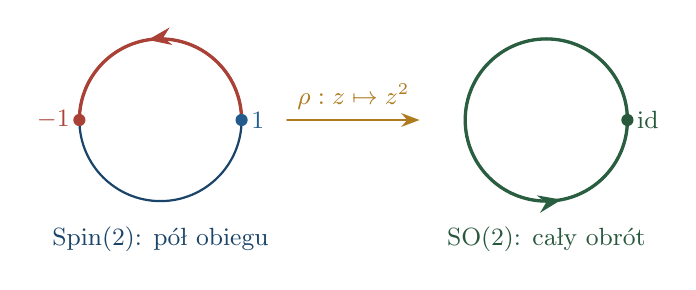
\begin{tikzpicture}[>=Stealth,line cap=round]
 \draw[manifoldblue!75!black,thick] (-2.45,0) circle (1.03);
 \draw[manifoldgreen!75!black,thick] (2.45,0) circle (1.03);
 \draw[manifoldred,very thick,postaction={decorate},
  decoration={markings,mark=at position .55 with {\arrow{Stealth}}}]
  (-1.42,0) arc[start angle=0,end angle=180,radius=1.03];
 \draw[manifoldgreen!75!black,very thick,postaction={decorate},
  decoration={markings,mark=at position .78 with {\arrow{Stealth}}}]
  (3.48,0) arc[start angle=0,end angle=360,radius=1.03];
 \fill[manifoldblue] (-1.42,0) circle (2.2pt)
  node[right,font=\small] {$1$};
 \fill[manifoldred] (-3.48,0) circle (2.2pt)
  node[left,font=\small] {$-1$};
 \fill[manifoldgreen!70!black] (3.48,0) circle (2.2pt)
  node[right,font=\small] {$\id$};
 \draw[->,thick,manifoldgold!85!black] (-.84,0)--(.84,0)
  node[midway,above,font=\small] {$\rho:z\mapsto z^2$};
 \node[font=\small,manifoldblue!75!black] at (-2.45,-1.52)
  {$\operatorname{Spin}(2)$: pół obiegu};
 \node[font=\small,manifoldgreen!70!black] at (2.45,-1.52)
  {$\mathrm{SO}(2)$: cały obrót};
\end{tikzpicture}
\caption{Droga od $1$ do $-1$ w $\operatorname{Spin}(2)$
rzutuje się na pełen obrót w $\mathrm{SO}(2)$.
Końce drogi są różne w grupie Spin, choć odpowiadają
temu samemu obrotowi.}
\label{fig:spin-dwukrotne}
\end{figure}

\begin{przyklad}[Trzy wymiary: kwaterniony]
\label{prz:spin3}
W $\operatorname{Cl}(\R^3)$ część parzysta ma bazę
$1,I=e_2e_3,J=e_3e_1,K=e_1e_2$.
Na przykład z \eqref{eq:cliff-orto}
$I^2=e_2e_3e_2e_3=-e_2^2e_3^2=-1$ oraz
$IJ=e_2e_3e_3e_1=-e_2e_1=e_1e_2=K$.
Cykliczna zamiana indeksów $1,2,3$ daje
$J^2=K^2=-1$, $JK=I$ i $KI=J$.
Iloczyny w odwrotnej kolejności mają przeciwne znaki;
na przykład $JI=e_3e_1e_2e_3=-e_1e_2=-K$.
Jest to algebra kwaternionów $\mathbb H$.
Odwracanie kolejności czynników wysyła
$a+bI+cJ+dK$ na $a-bI-cJ-dK$,
więc $s\widetilde s=a^2+b^2+c^2+d^2$.
Istotnie, dla $q=bI+cJ+dK$ mieszane składniki $q^2$
znikają, bo $IJ+JI=JK+KJ=KI+IK=0$.
Stąd $q^2=-(b^2+c^2+d^2)$ i
$(a+q)(a-q)=a^2-q^2$ daje tę równość.
Każdy element $\operatorname{Spin}(3)$
jest zatem jednostkowym kwaternionem.
I odwrotnie, dowolny jednostkowy kwaternion
można zapisać jako $\cos t+\sin t\,B$,
gdzie $B$ jest jednostkowym dwuwektorem
w $\R^3$ (przypadki $\pm1$ są natychmiastowe).
Każdy taki $B$ jest iloczynem dwóch
prostopadłych wektorów jednostkowych. Aby to sprawdzić,
zapiszmy $B=b e_2e_3+c e_3e_1+d e_1e_2$ z $b^2+c^2+d^2=1$.
Wybierzmy jednostkowy $u\perp n=(b,c,d)$ i połóżmy
$v=n\times u$. Wtedy $u,v$ są ortonormalne i $u\times v=n$.
Współczynniki $u\wedge v$ w bazie
$(e_2\wedge e_3,e_3\wedge e_1,e_1\wedge e_2)$ są właśnie $(b,c,d)$,
więc $uv=B$. Z kolei
$\cos t+\sin t\,B$ jest także iloczynem dwóch
wektorów jednostkowych: jeśli $B=uv$ dla
$u\perp v$, to wprost z $vu=-uv$ i $u^2=-1$
otrzymujemy
\[
 (-\cos t\,u-\sin t\,v)u
     =\cos t+\sin t\,uv.
\]
Zatem $\operatorname{Spin}(3)\cong S^3$
jako grupa jednostkowych kwaternionów,
a $\rho:S^3\to\mathrm{SO}(3)$ utożsamia
parę $s,-s$.
\end{przyklad}

\section{Spinory: moduły algebry Clifforda}
\label{sec:spinory}

Wektor w $\R^n$ obraca się przez $\rho(s)\in\mathrm{SO}(n)$.
Spinor ma podlegać działaniu samego $s\in\operatorname{Spin}(n)$,
tak aby dwa podniesienia tego samego obrotu mogły
działać odmiennie. Do opisania wszystkich wymiarów
użyjemy liczb zespolonych. \emph{Zespolenie}
$\operatorname{Cl}^{\C}_n:=
\operatorname{Cl}(\R^n)\otimes_\R\C$
ma tę samą bazę uporządkowanych słów co algebra
rzeczywista, ale współczynniki zespolone.
Jego wymiar nad $\C$ wynosi $2^n$.

\begin{definicja}[Spinor zespolony]
\index{spinor zespolony@Spinor zespolony}
\label{def:spinor}
\emph{Moduł} algebry $A$ nad $\mathbb K$ to przestrzeń liniowa
$\Delta$ nad $\mathbb K$ z działaniem $A\times\Delta\to\Delta$
dwuliniowym nad $\mathbb K$ i zgodnym
z mnożeniem: $(ab)\psi=a(b\psi)$
oraz $1\psi=\psi$. Jest \emph{nieredukowalny},
jeśli $\Delta\ne0$ i nie ma właściwej niezerowej podprzestrzeni
zachowywanej przez wszystkie działania $a\in A$.
W tym rozdziale \emph{przestrzenią spinorów}
w wymiarze $n$ nazwiemy nieredukowalny zespolony
moduł $\Delta_n$ algebry $\operatorname{Cl}^{\C}_n$.
Jej element $\psi$ to spinor. Ograniczenie
działania do $\operatorname{Spin}(n)\subset
\operatorname{Cl}^{\C}_n$ jest
\emph{reprezentacją spinową}.
\end{definicja}

Słowo \emph{moduł} brzmi abstrakcyjnie, lecz tutaj
oznacza po prostu konkretne macierze $c(v)$
działające na kolumny $\psi$, z warunkiem
$c(v)^2=-\|v\|^2 I$. Działanie na całej algebrze
jest wtedy wyznaczone przez jej własność uniwersalną.
Przykładem modułu jest $\Lambda V$ z dowodu
Twierdzenia~\ref{thm:cliff-baza}, ale zwykle jest
on \emph{większy} niż nieredukowalna przestrzeń
spinorów. Nie należy więc utożsamiać automatycznie
wielowektora ze spinorem.

\begin{przyklad}[Macierze Pauliego]
\label{prz:pauli}
Niech
\[
 \sigma_1=\begin{pmatrix}0&1\\1&0\end{pmatrix},
 \quad
 \sigma_2=\begin{pmatrix}0&-i\\i&0\end{pmatrix},
 \quad
 \sigma_3=\begin{pmatrix}1&0\\0&-1\end{pmatrix}.
\]
Kwadraty $\sigma_1,\sigma_3$ są identycznością,
a dla $\sigma_2$ dwa diagonalne współczynniki kwadratu
to $(-i)i=i(-i)=1$, przy zerowych pozostałych.
Trzy niezależne iloczyny różnych macierzy wynoszą
\[
 \begin{aligned}
 \sigma_1\sigma_2&=\begin{pmatrix}i&0\\0&-i\end{pmatrix}
                  =i\sigma_3,\\
 \sigma_2\sigma_3&=\begin{pmatrix}0&i\\i&0\end{pmatrix}
                  =i\sigma_1,\\
 \sigma_3\sigma_1&=\begin{pmatrix}0&1\\-1&0\end{pmatrix}
                  =i\sigma_2.
 \end{aligned}
\]
Każda $\sigma_j$ jest hermitowska.
Sprzężenie tych trzech równości daje więc iloczyny w odwrotnej
kolejności: $(\sigma_i\sigma_j)^*=\sigma_j\sigma_i$,
a $(i\sigma_k)^*=-i\sigma_k$.
Otrzymaliśmy $\sigma_i^2=I_2$ oraz
$\sigma_i\sigma_j=-\sigma_j\sigma_i$ dla $i\ne j$.
Macierze $c(e_j)=i\sigma_j$ spełniają więc
\[
 c(e_i)c(e_j)+c(e_j)c(e_i)=-2\delta_{ij}I_2.
\]
Dla $n=2$ wystarczą $c(e_1),c(e_2)$.
Ich iloczyn to $-i\sigma_3$, a cztery macierze
$I_2,i\sigma_1,i\sigma_2,-i\sigma_3$
są liniowo niezależne i rozpinają
$M_2(\C)$. Aby sprawdzić niezależność, przyrównujemy
ich kombinację do macierzy zerowej:
\[
 \alpha I_2+\beta i\sigma_1+\gamma i\sigma_2-\delta i\sigma_3
 =\begin{pmatrix}
   \alpha-i\delta&i\beta+\gamma\\
   i\beta-\gamma&\alpha+i\delta
  \end{pmatrix}=0.
\]
Dodanie i odjęcie równań diagonalnych daje
$\alpha=\delta=0$, a pozostałych $\beta=\gamma=0$.
W przestrzeni wymiaru $4$ te cztery macierze tworzą więc bazę.
Z wymiaru $4$ obu stron dostajemy
$\operatorname{Cl}^{\C}_2\cong M_2(\C)$.
Przestrzeń spinorów $\Delta_2=\C^2$
jest zwykłą przestrzenią kolumn długości $2$.
\end{przyklad}

\begin{twierdzenie}[Klasyfikacja zespolona i wymiar spinorów]
\label{thm:cliff-kompleks}
Dla $m\geq0$ istnieją izomorfizmy algebr
\begin{align}
 \operatorname{Cl}^{\C}_{2m}
   &\cong M_{2^m}(\C), \label{eq:cliff-complex-even}\\
 \operatorname{Cl}^{\C}_{2m+1}
   &\cong M_{2^m}(\C)\oplus M_{2^m}(\C).
   \label{eq:cliff-complex-odd}
\end{align}
Wobec tego nieredukowalny moduł zespolony
ma wymiar $2^{\lfloor n/2\rfloor}$.
Dla parzystego $n$ jest jeden taki moduł
z dokładnością do izomorfizmu, a dla
nieparzystego $n$ są dwa.
\end{twierdzenie}
\begin{proof}
W wymiarze $0$ algebra ma postać $\C$.
W wymiarze $1$ składa się z $a+be_1$ przy
$e_1^2=-1$. Homomorfizm
$a+be_1\mapsto(a+bi,a-bi)$ powstaje przez podstawienia
$e_1=i$ i $e_1=-i$.
Ma odwrotność
$(z_+,z_-)\mapsto(z_++z_-)/2+(z_+-z_-)\,e_1/(2i)$,
więc daje $\operatorname{Cl}^{\C}_1\cong\C\oplus\C$.
Przykład~\ref{prz:pauli} daje
$\operatorname{Cl}^{\C}_2\cong M_2(\C)$.

Wykażmy krok indukcyjny zwiększający wymiar o $2$.
Iloczyn tensorowy algebr wyposażamy tu w mnożenie
$(a\otimes A)(b\otimes B)=ab\otimes AB$, rozszerzone
dwuliniowo; własność uniwersalna iloczynu tensorowego zapewnia
jego poprawne określenie. Łączność sprawdzamy na tensorach
prostych, a jedynką jest $1\otimes I_2$.
Niech $e_1,\ldots,e_n$ będą generatorami
$\operatorname{Cl}^{\C}_n$. W algebrze
$\operatorname{Cl}^{\C}_n\otimes M_2(\C)$
weźmy $n+2$ elementów:
\[
 F_j=e_j\otimes\sigma_3\ (j\leq n),\qquad
 F_{n+1}=1\otimes i\sigma_1,\qquad
 F_{n+2}=1\otimes i\sigma_2.
\]
Każdy $F_j^2=-1$. Dwa różne elementy
antykomutują: dla $j,\ell\leq n$ wynika
to z relacji starych $e_j$; między pierwszymi
$n$ a ostatnimi dwoma wynika z tego, że
$\sigma_3$ antykomutuje z $\sigma_1,\sigma_2$;
ostatnie dwa antykomutują jako macierze Pauliego.
Własność uniwersalna daje homomorfizm
\[
 \operatorname{Cl}^{\C}_{n+2}
    \longrightarrow
   \operatorname{Cl}^{\C}_n\otimes M_2(\C).
\]
Obrazy dwóch ostatnich generatorów dają całą
podalgebrę $1\otimes M_2(\C)$:
ich iloczyn jest $-i(1\otimes\sigma_3)$,
a wraz z jedynką tworzą bazę czterech macierzy.
Następnie z
$(e_j\otimes\sigma_3)(1\otimes\sigma_3)
=e_j\otimes I_2$ otrzymujemy wszystkie
generatory pierwszego czynnika. Homomorfizm
jest więc surjektywny. Obie algebry mają
wymiar $2^{n+2}$ nad $\C$
(Twierdzenie~\ref{thm:cliff-baza}),
więc jest izomorfizmem. Używamy przy tym
$M_d(\C)\otimes M_2(\C)\cong M_{2d}(\C)$:
jednostka macierzowa $E_{ab}\otimes E_{rs}$ odpowiada
jednostce z indeksem wiersza $(a,r)$ i kolumny $(b,s)$.
To bijekcja baz zachowująca mnożenie. Iloczyn tensorowy
rozdziela się też względem sumy prostej obu składników.
Iteracja od $n=0$
i $n=1$ daje~\eqref{eq:cliff-complex-even}
i~\eqref{eq:cliff-complex-odd}.

Pozostaje uzasadnić wymiary modułów. Algebra
$M_d(\C)$ działa na $\C^d$ nieredukowalnie:
jeśli podprzestrzeń zawiera $x\ne0$, to
dla dowolnego $y\in\C^d$ można znaleźć
macierz $A$ z $Ax=y$, więc zawiera wszystkie $y$.
Każdy nieredukowalny moduł $M_d(\C)$ jest
izomorficzny z tym standardowym: wybieramy
wektor $\psi$ z $E_{11}\psi\ne0$ (w razie potrzeby
zmieniamy indeks; jest to możliwe, gdyż
$\sum_jE_{jj}=I$). Wektory
$E_{i1}\psi$, $1\leq i\leq d$, są liniowo
niezależne: zastosowanie $E_{1j}$ do ich
kombinacji liniowej zerowej pozostawia
tylko $j$-ty współczynnik razy
$E_{11}\psi\ne0$. Ich rozpiętość zachowują
wszystkie macierze, bo
$E_{ab}(E_{i1}\psi)=\delta_{bi}E_{a1}\psi$.
Jest zatem niezerowym podmodułem, a
nieredukowalność wymusza, że stanowi cały moduł.
Dla sumy dwóch algebr macierzowych jej
dwa centralne idempotenty $(I,0)$, $(0,I)$
rozkładają każdy moduł na dwie niezmiennicze
części. W module nieredukowalnym tylko jedna
z nich jest niezerowa, co daje dokładnie
dwa wybory modułu wymiaru $d$.
\end{proof}

\begin{uwaga}[Dwa moduły w wymiarze nieparzystym]
Gdy $n=2m+1\geq3$, dwa nieredukowalne moduły
$\operatorname{Cl}^{\C}_n$ są różne, lecz
po ograniczeniu do $\operatorname{Spin}(n)$
dają izomorficzne reprezentacje.
Rzeczywiście, podalgebra parzysta jest
izomorficzna z
$\operatorname{Cl}^{\C}_{n-1}$: przypiszmy
jego generatorowi $e_j$ element $e_je_n$
dla $j<n$. Dla $j,\ell<n$ obliczamy
$(e_je_n)(e_\ell e_n)=-e_je_\ell e_n^2=e_je_\ell$.
Dla $j=\ell$ daje to kwadrat $-1$, a dla $j\ne\ell$
zamiana $j,\ell$ zmienia znak. Te elementy zatem antykomutują i
generują wszystkie parzyste słowa
(każde $e_je_\ell$ z $j,\ell<n$ jest dokładnie
iloczynem $(e_je_n)(e_\ell e_n)$). Obie strony mają
wymiar $2^{n-1}$, więc to izomorfizm.
Ponieważ $n-1=2m$, algebra parzysta jest
$M_{2^m}(\C)$ i ma tylko jeden nieredukowalny
moduł. Trzeba jeszcze sprawdzić nieredukowalność ograniczeń:
każdy z dwóch modułów ma wymiar $d=2^m$, a w dowolnym
niezerowym module $M_d(\C)$ konstrukcja z jednostkami $E_{ij}$
z poprzedniego dowodu daje podmoduł wymiaru $d$.
Tutaj musi on być całą przestrzenią. Ponadto słowa parzyste
z wektorów ortonormalnych należą do Spin i rozpinają algebrę
parzystą, więc niezmienniczość względem Spin jest równoważna
niezmienniczości względem tej algebry.
W szczególności spinor dla obrotów
wymiaru $3$ ma po prostu dwie zespolone składowe.
Można zobaczyć oba działania Clifforda na tej samej przestrzeni:
jeśli $c_+(v)$ jest jednym z nich, to $c_-(v)=-c_+(v)$
na wektorach. Zmiana znaku każdego słowa nieparzystego
zamienia dwa nieredukowalne moduły, natomiast na słowach
parzystych, a więc i na grupie Spin, działania są identyczne.
Rozróżnia je centralny element
$i^{m+1}e_1\cdots e_{2m+1}$.
Przeniesienie generatora przez $2m$ pozostałych nie zmienia
znaku, co wyjaśnia centralność.
Kwadrat iloczynu $n$ różnych generatorów to
$(-1)^{n(n-1)/2}(-1)^n=(-1)^{n(n+1)/2}$:
pierwszy znak pochodzi od ich uporządkowania, drugi od kwadratów.
Dla $n=2m+1$ wynosi $(-1)^{m+1}$.
Czynnik $i^{m+1}$ ma kwadrat również równy $(-1)^{m+1}$,
więc cały element ma kwadrat $1$.
Zmiana znaków nieparzystej liczby generatorów zmienia jego znak
i zamienia wartości własne.
\end{uwaga}

\begin{stwierdzenie}[Spinory chiralne w wymiarze parzystym]
\label{prop:spin-chiral}
Dla $n=2m\geq2$ ustalmy orientację $V$ i dodatnią bazę
ortonormalną $(e_1,\ldots,e_{2m})$. W module $\Delta_{2m}$
element
\[
 \Gamma:=i^m c(e_1e_2\cdots e_{2m})
\]
ma własność $\Gamma^2=I$, komutuje z działaniem
$\operatorname{Spin}(2m)$ i dzieli przestrzeń
na dwa nieredukowalne, nieizomorficzne podmoduły dla grupy Spin:
\[
 \Delta_{2m}=\Delta^+_{2m}\oplus\Delta^-_{2m},
 \qquad
 \Delta^\pm_{2m}=\ker(\Gamma\mp I),\qquad
 \dim_\C\Delta^\pm_{2m}=2^{m-1}.
\]
Nazywamy je \emph{półspinorami}.
\end{stwierdzenie}
\begin{proof}
Niech $\omega=e_1\cdots e_{2m}$. Aby uporządkować czynniki
w iloczynie $\omega^2$, wykonujemy $(2m)(2m-1)/2$ transpozycji;
następnie mnożymy $2m$ kwadratów $e_j^2=-1$.
Otrzymujemy
$\omega^2=(-1)^{m(2m-1)}(-1)^{2m}=(-1)^m$.
Ponieważ $i^{2m}=(-1)^m$, mamy $\Gamma^2=I$.
Zatem $P_\pm=\tfrac12(I\pm\Gamma)$ są projekcjami
o sumie $I$ i zerowym iloczynie; dają podany rozkład na przestrzenie własne.
Zmiana dodatniej bazy ortonormalnej nie zmienia $\omega$.
Istotnie, wyrażenie
\[
 \operatorname{Alt}(v_1,\ldots,v_{2m})
 :=\frac{1}{(2m)!}
   \sum_{\pi\in S_{2m}}\operatorname{sgn}(\pi)\,
    v_{\pi(1)}\cdots v_{\pi(2m)}
\]
jest naprzemienne i wieloliniowe, a na bazie ortonormalnej
równa się jej iloczynowi Clifforda, bo wszystkie różne
wektory bazy antykomutują. Jako odwzorowanie naprzemienne
przy zmianie bazy mnoży się przez wyznacznik, tutaj równy $1$.
Przy odwróceniu orientacji $\Gamma$ zmienia znak i oznaczenia
$\Delta^+$, $\Delta^-$ zamieniają się miejscami.
Przesunięcie dowolnego $e_j$ przez pozostałe
$2m-1$ generatory zmienia znak:
$\Gamma c(e_j)=-c(e_j)\Gamma$.
Przez liniowość to samo zachodzi dla $c(v)$ każdego $v\in V$,
więc mnożenie Clifforda przez wektor zamienia oba półspinory.
Zatem $\Gamma$ komutuje z iloczynami
parzystej liczby generatorów, w szczególności
ze $\operatorname{Spin}(2m)$; obie przestrzenie
własne są niezmiennicze. Operator
$c(e_1)$ jest odwracalny i przestawia
te przestrzenie własne, więc mają równe
wymiary. Suma wymiarów to $2^m$ z poprzedniego
twierdzenia, co daje $2^{m-1}$.

Sprawdźmy jeszcze nieredukowalność względem grupy Spin.
Jeśli $0\ne W\subset\Delta^+_{2m}$ jest jej niezmienniczą
podprzestrzenią, to $W\oplus c(e_1)W$ jest niezmiennicza
względem każdego $c(e_j)$: istotnie,
$c(e_1)^{-1}c(e_j)$ oraz $c(e_j)c(e_1)$ są działaniami
elementów Spin (dla $j=1$ pierwszy z nich to $I$).
Stąd $c(e_j)W\subset c(e_1)W$ i
$c(e_j)c(e_1)W\subset W$.
Przestrzeń ta jest więc niezerowym podmodułem całej algebry
Clifforda. Nieredukowalność $\Delta_{2m}$ wymusza
$W\oplus c(e_1)W=\Delta_{2m}$, skąd $W=\Delta^+_{2m}$.
Tak samo postępujemy dla $\Delta^-_{2m}$.
Wreszcie $\omega=e_1\cdots e_{2m}\in\operatorname{Spin}(2m)$
działa na tych przestrzeniach przez różne skalary
$i^{-m}$ i $-i^{-m}$. Żaden niezerowy operator splatający
oba działania grupy Spin nie może więc istnieć.
\end{proof}

\begin{przyklad}[Półspinory w płaszczyźnie]
Dla $n=2$ w modelu Pauliego
$\Gamma=i\,c(e_1)c(e_2)=\sigma_3$,
więc $\Delta^+_2=\C\binom10$ oraz
$\Delta^-_2=\C\binom01$.
Element $s_\theta$ z Przykładu~\ref{prz:spin2}
działa przez
$c(s_\theta)=\cos(\theta/2)I_2
+\sin(\theta/2)c(e_1)c(e_2)
=\cos(\theta/2)I_2-i\sin(\theta/2)\sigma_3$.
Ponieważ $\sigma_3=\operatorname{diag}(1,-1)$,
oba współczynniki diagonalne to
$\cos(\theta/2)\mp i\sin(\theta/2)=e^{\mp i\theta/2}$.
Zatem
\[
 c(s_\theta)=
 \begin{pmatrix}
  e^{-i\theta/2}&0\\0&e^{i\theta/2}
 \end{pmatrix}.
\]
Wektor po obrocie o $2\pi$ wraca do swego
położenia, a każdy z obu półspinorów
zostaje przemnożony przez $-1$.
\end{przyklad}

\begin{przyklad}[Spinor w $\R^3$ i sfera Blocha]
\label{prz:bloch}
W wymiarze $3$ działanie
$c(e_j)=i\sigma_j$ na $\Delta_3=\C^2$
spełnia relacje Clifforda. Na parzystych
generatorach z Przykładu~\ref{prz:spin3}
otrzymujemy macierze $-i\sigma_1,-i\sigma_2,
-i\sigma_3$. Dla
$s=a+bI+cJ+dK\in\operatorname{Spin}(3)$
macierz działania ma postać
\[
 U_s=aI_2-i(b\sigma_1+c\sigma_2+d\sigma_3).
\]
Połóżmy $H=b\sigma_1+c\sigma_2+d\sigma_3$.
Macierze Pauliego są hermitowskie, więc $H^*=H$.
W rozwinięciu $H^2$ składniki mieszane kasują się parami,
bo $\sigma_j\sigma_k+\sigma_k\sigma_j=0$ dla $j\ne k$,
a $\sigma_j^2=I_2$. Stąd
\[
 U_s^*U_s=(aI_2+iH)(aI_2-iH)
 =a^2I_2+H^2=(a^2+b^2+c^2+d^2)I_2=I_2.
\]
Podstawiając macierze Pauliego, dostajemy również
\[
 U_s=\begin{pmatrix}a-id&-c-ib\\c-ib&a+id\end{pmatrix},
 \qquad
 \det U_s=(a^2+d^2)-(-c^2-b^2)=1.
\]
Sprawdźmy teraz, że tak otrzymujemy każdą macierz $U\in\mathrm{SU}(2)$.
Jej pierwsza kolumna $(\alpha,\gamma)^T$ ma normę $1$,
a jednostkowe wektory do niej prostopadłe to
$\lambda(-\overline\gamma,\overline\alpha)^T$, $|\lambda|=1$.
Druga kolumna ma więc tę postać. Wyznacznik takiej macierzy
wynosi $\lambda(|\alpha|^2+|\gamma|^2)=\lambda$,
zatem warunek $\det U=1$ wymusza $\lambda=1$.
Pisząc $\beta=-\overline\gamma$, otrzymujemy
$U=\begin{psmallmatrix}\alpha&\beta\\
-\overline\beta&\overline\alpha\end{psmallmatrix}$,
gdzie $|\alpha|^2+|\beta|^2=1$.
Porównanie współczynników daje jednoznacznie
$a=\Re\alpha$, $d=-\Im\alpha$,
$c=-\Re\beta$, $b=-\Im\beta$;
warunek normy kolumny to właśnie $a^2+b^2+c^2+d^2=1$.
Zatem $\operatorname{Spin}(3)\cong\mathrm{SU}(2)$.

Niech teraz $\psi=(z_1,z_2)^T$ ma normę $1$.
Liczby rzeczywiste
\begin{equation}\label{eq:spin-bloch}
 b_j(\psi):=\psi^*\sigma_j\psi
 \quad\text{dają}\quad
 b(\psi)=
 \bigl(2\Re(\overline z_1z_2),
       2\Im(\overline z_1z_2),
       |z_1|^2-|z_2|^2\bigr).
\end{equation}
Wyprowadźmy te współrzędne. Dla $w=\overline z_1z_2$
mnożenie przez $\sigma_1$ daje
$\psi^*\sigma_1\psi=w+\overline w=2\Re w$,
a przez $\sigma_2$ daje
$\psi^*\sigma_2\psi=-iw+i\overline w=2\Im w$.
Macierz diagonalna $\sigma_3$ daje różnicę kwadratów modułów.
Ponieważ $(\Re w)^2+(\Im w)^2=|w|^2$, mamy
\[
 \begin{aligned}
 \|b(\psi)\|^2
 &=4|z_1|^2|z_2|^2+(|z_1|^2-|z_2|^2)^2\\
 &=(|z_1|^2+|z_2|^2)^2=1.
 \end{aligned}
\]
Zmiana fazy $\psi\mapsto e^{i\varphi}\psi$
nie zmienia $b(\psi)$: w każdym iloczynie
$\overline z_jz_k$ czynniki fazowe się skracają.
Odwrotnie, liczby $b_j$ wyznaczają macierz
\[
 \begin{aligned}
 \psi\psi^*
 &=\begin{pmatrix}
 |z_1|^2&z_1\overline z_2\\
 z_2\overline z_1&|z_2|^2
 \end{pmatrix}\\
 &=\frac12\begin{pmatrix}
 1+b_3&b_1-ib_2\\b_1+ib_2&1-b_3
 \end{pmatrix}
 =\frac12\left(I_2+\sum_{j=1}^3b_j\sigma_j\right).
 \end{aligned}
\]
Jest to rzut ortogonalny na $\C\psi$: wysyła $v$ na
$\psi(\psi^*v)$ i zachowuje $\psi$, bo $\psi^*\psi=1$.
Jego obraz wyznacza zatem tę prostą jednoznacznie.
Każdy punkt sfery otrzymujemy: dla
$b=(x,y,z)$ z $z>-1$ bierzemy
$z_1=\sqrt{(1+z)/2}$,
$z_2=(x+iy)/\sqrt{2(1+z)}$;
dla bieguna południowego bierzemy $(0,1)$.
Istotnie, $x^2+y^2=1-z^2$ daje
$|z_2|^2=(x^2+y^2)/(2(1+z))=(1-z)/2$,
więc $|z_1|^2+|z_2|^2=1$ oraz $|z_1|^2-|z_2|^2=z$.
Ponadto $\overline z_1z_2=(x+iy)/2$,
co odtwarza dwie pierwsze współrzędne we wzorze~\eqref{eq:spin-bloch}.
Otrzymujemy więc konkretną identyfikację
\[
 \mathbb{CP}^1=\operatorname{Gr}_1(\C^2)\cong S^2.
\]
Jest to także gładka identyfikacja: na mapie $[1:w]$
wybieramy jednostkowego przedstawiciela
$\psi=(1,w)^T/\sqrt{1+|w|^2}$.
Podstawienie go do~\eqref{eq:spin-bloch} daje
$b=(2\Re w,2\Im w,1-|w|^2)/(1+|w|^2)$,
a odwrotność poza biegunem południowym to $w=(x+iy)/(1+z)$;
druga mapa analogicznie obsługuje biegun południowy.
Macierze $U_s$ obracają odpowiedni punkt sfery.
Istotnie, z $U_sc(v)U_s^{-1}=c(\rho(s)v)$ i $c(v)=i\sum_jv_j\sigma_j$
otrzymujemy
\[
 (U_s\psi)(U_s\psi)^*
 =U_s\psi\psi^*U_s^{-1}
 =\tfrac12\bigl(I_2+\textstyle\sum_j(\rho(s)b(\psi))_j\sigma_j\bigr).
\]
Jednoznaczność współczynników przy $\sigma_j$ daje
$b(U_s\psi)=\rho(s)b(\psi)$.
Znak spinora $\psi\mapsto-\psi$ jest
niewidoczny po przejściu do punktu sfery.
\end{przyklad}

\begin{figure}[!htbp]
\centering
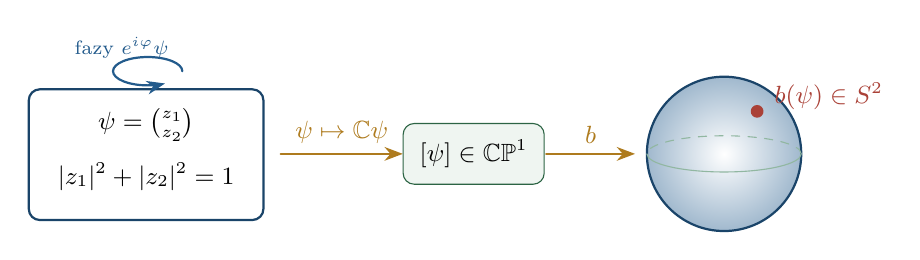
\begin{tikzpicture}[>=Stealth,line cap=round,scale=1.0]
 \draw[manifoldblue!75!black,thick,rounded corners]
 (-5.6,-.72) rectangle (-2.62,.94);
 \node[font=\small] at (-4.11,.49)
   {$\psi=\binom{z_1}{z_2}$};
 \node[font=\small] at (-4.11,-.17)
   {$|z_1|^2+|z_2|^2=1$};
 \draw[->,manifoldblue,thick] (-3.65,1.17)
  arc[start angle=0,end angle=300,x radius=.44,y radius=.18];
 \node[font=\scriptsize,manifoldblue] at (-4.42,1.47)
  {fazy $e^{i\varphi}\psi$};
 \draw[->,thick,manifoldgold!85!black] (-2.4,.12)--(-.85,.12)
  node[midway,above,font=\small] {$\psi\mapsto\C\psi$};
 \node[draw=manifoldgreen!80!black,rounded corners,
  fill=manifoldgreen!8,font=\small,inner sep=6pt] at (.05,.12)
  {$[\psi]\in\mathbb{CP}^1$};
 \draw[->,thick,manifoldgold!85!black] (.97,.12)--(2.1,.12)
  node[midway,above,font=\small] {$b$};
 \shade[inner color=white,outer color=manifoldblue!43] (3.23,.12) circle (.98);
 \draw[manifoldblue!75!black,thick] (3.23,.12) circle (.98);
 \draw[manifoldgreen!55,thin] (2.25,.12)
   arc[start angle=180,end angle=360,x radius=.98,y radius=.23];
 \draw[manifoldgreen!55,thin,dashed] (4.21,.12)
   arc[start angle=0,end angle=180,x radius=.98,y radius=.23];
 \fill[manifoldred] (3.65,.66) circle (2.3pt);
 \node[manifoldred,font=\small] at (4.56,.85) {$b(\psi)\in S^2$};
\end{tikzpicture}
\caption{Spinor jednostkowy $\psi\in\C^2$ ma fazę,
która nie zmienia prostej $[\psi]\in\mathbb{CP}^1$.
Wzór~\eqref{eq:spin-bloch} przypisuje tej prostej
punkt sfery. To łączy spinory z grassmannianem prostych.}
\label{fig:spin-bloch}
\end{figure}

\section{Struktury spinowe i wiązki spinorów}
\label{sec:struktura-spinowa}

\noindent\emph{Powiązania tematyczne w Bibliotece matematycznej:} \atlasref{LA-31::def:lin31-struktura-spinowa}{LA-31: struktura spinowa}.


Dotąd wektory, obroty i spinory należały do jednej
ustalonej przestrzeni $\R^n$. Na rozmaitości
przestrzeń $T_pM$ zmienia się z $p$.
Gładka rodzina dodatnio określonych iloczynów
skalarnych $g_p$ na $T_pM$ to \emph{metryka
riemannowska}. Pozwala wybierać bazy ortonormalne
w każdym punkcie. Jeśli $M$ jest zorientowana,
możemy wybierać bazy o dodatniej orientacji.

\emph{Wiązka dodatnio zorientowanych ramek
ortonormalnych} $F^+(M)\to M$ ma w punkcie $p$
za włókno wszystkie uporządkowane bazy
$(u_1,\ldots,u_n)$ przestrzeni $T_pM$,
które są ortonormalne i dodatnie.
Grupa $\mathrm{SO}(n)$ działa z prawej strony
przez zmianę takiej bazy. Nie ma wyróżnionej
bazy w każdym włóknie; lokalnie wiązka wygląda
jednak jak $U\times\mathrm{SO}(n)$.
Wiązkę o takiej lokalnej postaci, z wolnym
działaniem grupy przechodzącym tranzytywnie
na każdym włóknie, nazywamy \emph{wiązką główną}.

\begin{definicja}[Struktura spinowa i wiązka spinorowa]
\index{struktura spinowa i wiazka spinorowa@Struktura spinowa i wiązka spinorowa}
\label{def:struktura-spinowa}
Dla zorientowanej rozmaitości riemannowskiej
$M^n$, $n\geq2$, \emph{struktura spinowa}
składa się z wiązki głównej
$P_{\mathrm{Spin}}\to M$ o grupie
$\operatorname{Spin}(n)$ oraz odwzorowania
gładkiego $\lambda:P_{\mathrm{Spin}}\to F^+(M)$
nad identycznością bazy, takiego że
\[
 \lambda(pg)=\lambda(p)\rho(g),
 \qquad g\in\operatorname{Spin}(n),
\]
a $\lambda$ ograniczona do każdego włókna
jest dwukrotnym nakryciem.
Niech $\varrho:\operatorname{Spin}(n)\to\operatorname{GL}(\Delta_n)$
będzie ograniczeniem działania modułu Clifforda do grupy Spin.
\emph{Wiązka spinorowa} to wiązka zespolona
\[
 S:=P_{\mathrm{Spin}}\times_{\varrho}\Delta_n.
\]
Jej elementami są klasy par $(p,\psi)$,
$p\in P_{\mathrm{Spin}}$, $\psi\in\Delta_n$,
z relacją $(pg,\psi)\sim(p,\varrho(g)\psi)$.
\emph{Polem spinorowym} nazywamy gładki przekrój $S$.
Tę samą definicję stosujemy do dowolnej zorientowanej wiązki
euklidesowej $E$ rzędu $n$, zastępując $F^+(M)$ wiązką jej
dodatnich ramek ortonormalnych $F^+(E)$.
\end{definicja}

Po wyborze lokalnej ramki spinowej $s_i:U_i\to P_{\mathrm{Spin}}$
wiązka $S$ wygląda jak $U_i\times\Delta_n$. Ustalmy kierunek
zmian: jeśli $s_j=s_i h_{ij}$, to
$[s_j,\psi_j]=[s_i,c(h_{ij})\psi_j]$, zatem współrzędne
tego samego spinora spełniają $\psi_i=c(h_{ij})\psi_j$.
Przy przejściu od kolumny $i$ do kolumny $j$ używamy więc
macierzy odwrotnej. Z równości dla lokalnych ramek wynika też
$h_{ij}h_{jk}=h_{ik}$; reprezentacja $c$ przenosi tę równość
na macierze przejścia, co uzasadnia strukturę wiązki wektorowej $S$.
Wiązka spinorów ma ponadto \emph{mnożenie Clifforda przez wektory
styczne}. Dla $v\in T_xM$, $p\in(P_{\mathrm{Spin}})_x$ i
ramki $\lambda(p)$ traktowanej jako izometria
$f_p:\R^n\to T_xM$ określmy
\begin{equation}\label{eq:spin-bundle-cliff}
 c_x(v)[p,\psi]
   :=[p,c(f_p^{-1}v)\psi].
\end{equation}
Sprawdźmy niezależność od reprezentanta klasy. Gdy $p'=pg$,
to $f_{p'}=f_p\rho(g)$, a $[p',\psi']=[p,c(g)\psi']$.
Oznaczając $w=f_p^{-1}v$, dostajemy
\[
 [p',c(f_{p'}^{-1}v)\psi']
 =[p,c(g)c(\rho(g)^{-1}w)\psi']
 =[p,c(w)c(g)\psi'].
\]
Druga równość wynika z relacji
$c(g)c(u)c(g)^{-1}=c(\rho(g)u)$.
Zatem wzór~\eqref{eq:spin-bundle-cliff} jest dobrze określony,
zależy gładko od $x$ i spełnia
$c_x(v)^2=-g_x(v,v)I_{S_x}$.
W wymiarze parzystym $\Gamma$ jest niezmienniczy przy zmianie
dodatniej ramki, więc definiuje globalny rozkład
$S=S^+\oplus S^-$; mnożenie przez wektor zamienia $S^+$ z $S^-$.
Gdy chce się mnożyć przez kowektory, najpierw używa się metryki
do identyfikacji $T_x^*M\cong T_xM$.
W przypadku ogólnej wiązki $E$ w tym samym wzorze zastępujemy
$T_xM$ przez $E_x$.
W nieparzystym wymiarze dwa wybory nieredukowalnego działania
Clifforda dają równoważne działanie Spin na $S$, lecz w tym
utożsamieniu zmieniają znak mnożenia przez pojedynczy wektor.
Zauważmy też, że $\lambda$ jest nakryciem całych przestrzeni:
w lokalnej trywializacji zadanej przez $s_i$ i ramkę $\lambda\circ s_i$
ma postać $(x,g)\mapsto(x,\rho(g))$.
Jeśli zmiana ramki wektorowej wykonuje pełny
obrót o $2\pi$, jej podniesienie w Spin
może dojść do $-1$. Wtedy wektory wracają
do wartości początkowych, lecz spinor dostaje
znak minus. To lokalna treść różnicy między
wiązką wektorów i wiązką spinorów.

\begin{przyklad}[Płaszczyzna i sfera są spinowe]
Na $\R^n$ standardowe ramki dają
$F^+(\R^n)\cong\R^n\times\mathrm{SO}(n)$.
Bierzemy
$P_{\mathrm{Spin}}=\R^n\times\operatorname{Spin}(n)$
i $\lambda(x,s)=(x,\rho(s))$; spinory
tworzą trywialną wiązkę
$S\cong\R^n\times\Delta_n$.

Na sferze $S^2\subset\R^3$ każda dodatnia
ramka styczna $(u,v)$ w punkcie $p$ wyznacza
macierz o kolumnach $(u,v,p)\in\mathrm{SO}(3)$.
To utożsamia $F^+(S^2)$ z $\mathrm{SO}(3)$,
a rzut do bazy wysyła macierz na jej trzecią
kolumnę $p$. Dwukrotne nakrycie
$\mathrm{SU}(2)\cong\operatorname{Spin}(3)
\to\mathrm{SO}(3)$ z
Przykładu~\ref{prz:spin3} daje odwzorowanie $\lambda$.
Rzut z $\operatorname{Spin}(3)$ do sfery ma postać
$q(s)=\rho(s)e_3$. Używamy jednej, ustalonej podgrupy
$H=\rho^{-1}(\operatorname{Stab}(e_3))=\operatorname{Spin}(2)$,
złożonej z $\cos t+\sin t\,e_1e_2$. Działa ona z prawej strony
na $\operatorname{Spin}(3)$ i zachowuje $q(s)$.
Jeśli $q(s)=q(s')$, to $s^{-1}s'\in H$, więc działanie jest
wolne i przechodnie na każdym włóknie. Lokalne gładkie ramki
styczne $(u,v)$ dają lokalne sekcje w $\mathrm{SO}(3)$;
po zmniejszeniu otoczenia podnosimy je przez lokalną odwrotność
nakrycia $\rho$. To zapewnia lokalną trywialność wiązki głównej.
Równość $\lambda(sh)=\lambda(s)\rho(h)$ kończy sprawdzenie
definicji struktury spinowej na sferze.
\end{przyklad}

\begin{przyklad}[Cztery podniesienia ramek płaskiego torusa]
\label{prz:spin-torus}
Niech $T^2=\R^2/\Z^2$ ma metrykę płaską i orientację
zadaną przez stałą ramkę $(\partial_x,\partial_y)$.
W tej ramce $F^+(T^2)\cong T^2\times\mathrm{SO}(2)$.
Dla każdej pary znaków
$\varepsilon=(\varepsilon_1,\varepsilon_2)\in\{1,-1\}^2$
grupa $\Z^2$ działa na $\R^2\times\operatorname{Spin}(2)$ wzorem
\[
 (k_1,k_2)\cdot(x,s)
  =\bigl(x+(k_1,k_2),
          \varepsilon_1^{k_1}\varepsilon_2^{k_2}s\bigr).
\]
Iloraz $P_\varepsilon$ jest wiązką główną Spin:
nad małym kwadratem w torusie wybór jego podniesienia do $\R^2$
daje lokalną trywializację, a znaki są centralne,
więc działanie grupy Spin z prawej strony schodzi na iloraz.
Odwzorowanie
$\lambda_\varepsilon[x,s]=([x],\rho(s))$
jest dobrze określone, gdyż $\rho(\pm1)=I$.
Na każdym włóknie jest dwukrotnym nakryciem, zatem daje
strukturę spinową. Para $\varepsilon$ zapisuje znaki,
z jakimi podniesienie ustalonej stałej ramki wraca
po obejściu dwóch podstawowych pętli torusa.

Te cztery struktury są różne jako \emph{podniesienia}
ustalonej wiązki ramek. Istotnie, izomorfizm
$P_\varepsilon\to P_{\varepsilon'}$ zgodny z $\lambda$
po podciągnięciu do $\R^2$ ma postać
$(x,s)\mapsto(x,\delta(x)s)$, gdzie
$\delta(x)\in\ker\rho=\{\pm1\}$.
Funkcja $\delta$ jest stała, bo $\R^2$ jest spójna.
Porównanie identyfikacji punktów przy przesunięciach
o $(1,0)$ i $(0,1)$ wymusza więc
$\varepsilon_1=\varepsilon'_1$ oraz
$\varepsilon_2=\varepsilon'_2$.

Są to wszystkie struktury spinowe na torusie. Dla dowolnego
podniesienia $P\to F^+(T^2)$ podciągamy je do $\R^2$ i bierzemy
przeciwobraz stałej ramki. Jest to dwukrotne nakrycie
ściągalnej $\R^2$, więc ma gładką sekcję $\widetilde f$.
Po przesunięciu o $k\in\Z^2$ jej wartości nad tym samym
punktem torusa różnią się znakiem $\delta_k(x)\in\{\pm1\}$.
Ciągłość i spójność $\R^2$ czynią ten znak stałym w $x$,
a składanie przesunięć daje homomorfizm
$k\mapsto\delta_k$ z $\Z^2$ do $\{\pm1\}$.
Wyznaczają go dwa znaki dla $(1,0)$ i $(0,1)$;
trywializacja $(x,s)\mapsto\widetilde f(x)s$ utożsamia
wyjściowe podniesienie z odpowiednim $P_\varepsilon$.

W trywializacji spinorów podciągniętej do $\R^2$
pole spinorowe jest funkcją $\psi:\R^2\to\Delta_2$
spełniającą konkretne warunki
\[
 \psi(x+1,y)=\varepsilon_1\psi(x,y),
 \qquad
 \psi(x,y+1)=\varepsilon_2\psi(x,y).
\]
Wyprowadźmy te warunki z relacji ilorazowej.
Dla $k=(k_1,k_2)\in\Z^2$ oznaczmy
$\varepsilon^k=\varepsilon_1^{k_1}\varepsilon_2^{k_2}$.
Ramki spinowe nad tym samym punktem spełniają
$[x+k,1]=[x,\varepsilon^k]$.
W wiązce stowarzyszonej zastąpienie ramki $p$ przez $p h$
zastępuje współrzędną spinora przez $c(h)^{-1}$ razy tę współrzędną.
Zapis tego samego pola w obu ramkach wymaga więc
$\psi(x)=c(\varepsilon^k)\psi(x+k)$.
Z $c(-1)=-I_{\Delta_2}$ mamy
$c(\varepsilon^k)=\varepsilon^k I_{\Delta_2}$;
ponieważ $(\varepsilon^k)^2=1$, dostajemy
$\psi(x+k)=\varepsilon^k\psi(x)$.
Wybory $k=(1,0)$ i $k=(0,1)$ dają oba wypisane warunki.
Wybór znaku $-1$ oznacza więc antyperiodyczność
w odpowiednim kierunku, choć zwykłe wektory styczne
są okresowe w obu kierunkach.
\end{przyklad}

\begin{figure}[!htbp]
\centering
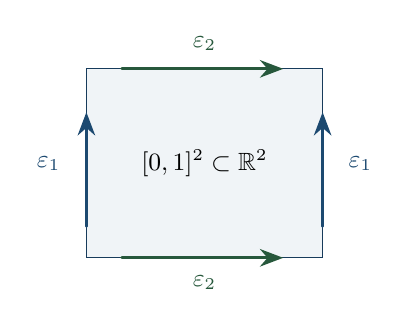
\begin{tikzpicture}[>=Stealth,line cap=round]
 \fill[manifoldblue!7] (0,0) rectangle (3,2.4);
 \draw[manifoldblue!65!black,thin] (0,0) rectangle (3,2.4);
 \draw[->,manifoldblue!80!black,very thick]
   (0,.4)--(0,1.85);
 \draw[->,manifoldblue!80!black,very thick]
   (3,.4)--(3,1.85);
 \draw[->,manifoldgreen!70!black,very thick]
   (.45,0)--(2.5,0);
 \draw[->,manifoldgreen!70!black,very thick]
   (.45,2.4)--(2.5,2.4);
 \node[font=\small,manifoldblue!80!black] at (-.48,1.2)
   {$\varepsilon_1$};
 \node[font=\small,manifoldblue!80!black] at (3.48,1.2)
   {$\varepsilon_1$};
 \node[font=\small,manifoldgreen!70!black] at (1.5,-.32)
   {$\varepsilon_2$};
 \node[font=\small,manifoldgreen!70!black] at (1.5,2.72)
   {$\varepsilon_2$};
 \node[font=\small] at (1.5,1.2) {$[0,1]^2\subset\R^2$};
\end{tikzpicture}
\caption{Dwie pary brzegów kwadratu fundamentalnego torusa.
Przesunięcie w kierunku $x$ utożsamia pionowe krawędzie
ze znakiem $\varepsilon_1$ dla spinora; przesunięcie w kierunku
$y$ utożsamia poziome krawędzie ze znakiem $\varepsilon_2$.
W wiązce ramek ortonormalnych oba znaki są niewidoczne.}
\label{fig:spin-torus-signs}
\end{figure}

\begin{uwaga}[Podnoszenie na zbiorze ściągalnym]
\label{rem:spin-podnoszenie}
Użyjemy elementarnego faktu o nakryciach: gładkie odwzorowanie
ze ściągalnego obszaru $U$ do podstawy gładkiego nakrycia ma
gładkie podniesienie po wybraniu obrazu jednego punktu.
Istotnie, drogę od tego punktu podnosimy kolejno przez lokalne
odwrotności nakrycia, dzieląc jej przedział parametrów na skończenie
wiele odcinków. Jednoznaczność na przecięciach daje jednoznaczność
podniesionej drogi. Homotopię dróg o ustalonych końcach podnosimy
analogicznie po podziale kwadratu parametrów na małe prostokąty,
których obrazy leżą w dziedzinach lokalnych odwrotności.
Końcowy punkt podniesienia nie zmienia się w tej homotopii:
poruszałby się ciągle w dyskretnym włóknie. W obszarze ściągalnym
każde dwie drogi o tych samych końcach są tak homotopijne,
więc ich podniesienia wyznaczają tę samą wartość w punkcie końcowym.
Otrzymana funkcja jest lokalnie złożeniem danej funkcji z jedną
lokalną odwrotnością nakrycia, zatem jest gładka.
Ten sam argument działa na dysku z brzegiem.
\end{uwaga}

\begin{przyklad}[Wiązka, której nie da się podnieść]
\label{prz:nie-spin-linia}
Podłoże $S^2\cong\mathbb{CP}^1$ jest spinowe,
ale nie każda \emph{wiązka} nad nim dopuszcza
podniesienie struktury do Spin.
Weźmy zespoloną wiązkę tautologiczną
$\gamma^1_\C$ nad
$\operatorname{Gr}_1(\C^2)=\mathbb{CP}^1$
i potraktujmy jej włókna jako rzeczywiste
zorientowane płaszczyzny wymiaru $2$.
Na mapie $[1:z]$ mamy ramkę zespoloną
$s_0(z)=(1,z)$, a na mapie $[w:1]$,
$w=1/z$, ramkę $s_\infty(w)=(w,1)$.
Na przecięciu
$s_\infty(1/z)=z^{-1}s_0(z)$.
Po unormowaniu ramek, przy $|z|=1$, $z=e^{i\theta}$, unitarny
czynnik przejścia jest więc $e^{-i\theta}$:
jako rzeczywista izometria obraca płaszczyznę
o kąt $-\theta$. Po przejściu
$0\leq\theta\leq2\pi$ daje pętlę
o nieparzystej liczbie pełnych obrotów.
Ta pętla w $\mathrm{SO}(2)$ nie ma
\emph{zamkniętego} podniesienia do $\operatorname{Spin}(2)$:
połowa kąta biegnie
od $0$ do $-\pi$ i kończy w $-1$, nie w $1$.
Gdyby istniała struktura spinowa, ramkę ortonormalną nad każdą
z dwóch półkul można by podnieść do ramki spinowej.
Rzeczywiście, przeciwobraz takiej ramki przez $\lambda$ jest
dwukrotnym nakryciem dysku; Uwagi~\ref{rem:spin-podnoszenie}
używamy do podniesienia identyczności dysku. Przejście między
otrzymanymi ramkami spinowymi na równiku byłoby właśnie
zamkniętym podniesieniem opisanej pętli, co jest sprzecznością.
Zmiana ramki na którejś z dwóch półkul
zmienia pętlę tylko o taką, która przedłuża
się na dysk i ma zerowy całkowity obrót.
Dlatego ten brak podniesienia nie zależy
od wybranych ramek. Wiązka rzeczywista otrzymana przez zapomnienie
struktury zespolonej $\gamma^1_\C$ nie ma struktury
spinowej, mimo że sama sfera $S^2$ ją ma.
\end{przyklad}

\begin{stwierdzenie}[Znaki na potrójnych przecięciach]
\label{prop:w2-znaki}
Niech $E$ będzie zorientowaną wiązką euklidesową
rzędu $n\geq2$ nad $M$. Weźmy dostatecznie drobne
pokrycie trywializujące $(U_i)$, w którym
niepuste skończone przecięcia są ściągalne. Takie pokrycie
nazywamy \emph{dobrym}; w tym stwierdzeniu zakładamy jego wybór.
Niech $g_{ij}:U_i\cap U_j\to\mathrm{SO}(n)$
przepisują współrzędne z trywializacji $j$ do trywializacji $i$,
więc $g_{ij}g_{jk}=g_{ik}$.
Na przecięciach wybierzmy podniesienia
$h_{ij}:U_i\cap U_j\to\operatorname{Spin}(n)$
z $\rho(h_{ij})=g_{ij}$ i $h_{ji}=h_{ij}^{-1}$.
Wtedy na potrójnym przecięciu
\begin{equation}\label{eq:w2-znaki}
 \varepsilon_{ijk}:=h_{ij}h_{jk}h_{ki}
          \in\{1,-1\}.
\end{equation}
Wiązka $E$ ma strukturę spinową dokładnie wtedy,
gdy wybory $h_{ij}$ można zmodyfikować znakami
tak, aby wszystkie $\varepsilon_{ijk}$ wynosiły $1$.
\end{stwierdzenie}
\begin{proof}
Z warunku kocyklu dla $g_{ij}$ mamy
$\rho(\varepsilon_{ijk})
=g_{ij}g_{jk}g_{ki}=I$.
Twierdzenie~\ref{thm:spin-nakrycie} mówi, że
jądro $\rho$ to $\{\pm1\}$; ponieważ znak jest
dyskretny, $\varepsilon_{ijk}$ jest lokalnie stały.
Nie ma problemu z samym podniesieniem
$g_{ij}$ na ściągalnym przecięciu:
zapewnia je Uwaga~\ref{rem:spin-podnoszenie}.
Przyjmujemy też $h_{ii}=1$.

Jeżeli na każdym potrójnym przecięciu
$\varepsilon_{ijk}=1$, to
$h_{ij}h_{jk}=h_{ik}$.
Są to funkcje przejścia z warunkiem kocyklu.
Sklejamy $U_i\times\operatorname{Spin}(n)$ relacją
$(x,a)_j\sim(x,h_{ij}(x)a)_i$. Warunek kocyklu zapewnia
przechodniość tej relacji, a gładkie przejścia zapewniają lokalne
trywializacje, jak w Sekcji~\ref{sec:wiazki-wektorowe}.
Działanie z prawej strony jest dobrze określone, wolne
i przechodnie we włóknach, więc otrzymujemy wiązkę główną.
Jeśli $f_i$ oznacza wybraną lokalną ramkę $E$, to
$\lambda([x,a]_i)=f_i(x)\rho(a)$ jest niezależne od reprezentanta,
ponieważ $f_j=f_i g_{ij}$ i $\rho(h_{ij})=g_{ij}$.
Lokalnie jest to $\id\times\rho$, a więc spełnia definicję
struktury spinowej.
Odwrotnie, w istniejącej strukturze spinowej podnosimy każdą
ustaloną ramkę $f_i$ do ramki spinowej nad ściągalnym $U_i$.
Stosujemy Uwagę~\ref{rem:spin-podnoszenie} do dwukrotnego
nakrycia będącego przeciwobrazem $f_i$ przez $\lambda$.
Przejścia tych ramek podnoszą właśnie dane $g_{ij}$ i spełniają
warunek kocyklu, więc wszystkie znaki są $1$.
Dowolne dwa odwzorowania $h_{ij}$ nad
tym samym $g_{ij}$ różnią się na spójnym
przecięciu stałym znakiem
$\delta_{ij}\in\{\pm1\}$.
Zmiana podniesień zastępuje
$\varepsilon_{ijk}$ przez
$\delta_{ij}\delta_{jk}\delta_{ki}
\varepsilon_{ijk}$, co dowodzi
sformułowania o modyfikacji znakami.
\end{proof}

\begin{uwaga}[Druga klasa Stiefela--Whitneya]
Zdarza się, że pojedynczych znaków
$\varepsilon_{ijk}$ nie da się wszystkich
usunąć. Ich układ spełnia warunek zgodności
na poczwórnych przecięciach. Z definicji znaków mamy
$h_{ij}h_{jk}=\varepsilon_{ijk}h_{ik}$.
Stosując tę równość do dwóch sposobów nawiasowania
iloczynu trzech przejść, otrzymujemy
\[
 \begin{aligned}
 (h_{ij}h_{jk})h_{k\ell}
 &=\varepsilon_{ijk}h_{ik}h_{k\ell}
 =\varepsilon_{ijk}\varepsilon_{ik\ell}h_{i\ell},\\
 h_{ij}(h_{jk}h_{k\ell})
 &=h_{ij}\varepsilon_{jk\ell}h_{j\ell}
 =\varepsilon_{jk\ell}\varepsilon_{ij\ell}h_{i\ell}.
 \end{aligned}
\]
W drugim wierszu użyto centralności znaku $\varepsilon_{jk\ell}$.
Łączność mnożenia i skrócenie odwracalnego $h_{i\ell}$
dają $\varepsilon_{ijk}\varepsilon_{ik\ell}
=\varepsilon_{jk\ell}\varepsilon_{ij\ell}$.
Taką rodzinę znaków nazywamy
\emph{dwukocyklowym} zapisem przeszkody.
Zmiany przez $\delta_{ij}$ z dowodu
uznajemy za równoważne. Nie zmienia tego wybór lokalnych ramek:
jeśli $f'_i=f_i a_i$, wybieramy podniesienia $b_i$ funkcji $a_i$
nad ściągalnymi $U_i$. Wtedy $g'_{ij}=a_i^{-1}g_{ij}a_j$
mają podniesienia $h'_{ij}=b_i^{-1}h_{ij}b_j$.
Ich iloczyn na potrójnym przecięciu to
$b_i^{-1}\varepsilon_{ijk}b_i=\varepsilon_{ijk}$,
bo znaki należą do centrum grupy Spin.
Wyjaśnijmy używane tutaj oznaczenie kohomologiczne,
aby nie odsyłać definicji przeszkody wyłącznie do
późniejszej teorii kohomologii. Utożsamiamy
$\{1,-1\}$ z grupą addytywną $\Z/2$ przez
$(-1)^a\longleftrightarrow a$.
Dla dobrego pokrycia $\mathcal U=(U_i)$
niech $C^q(\mathcal U;\Z/2)$ oznacza grupę rodzin
$a_{i_0\ldots i_q}\in\Z/2$, przypisanych
wszystkim niepustym przecięciom
$U_{i_0}\cap\cdots\cap U_{i_q}$ z rosnącymi indeksami.
Definiujemy \emph{operator kobrzegu}
$\delta:C^q(\mathcal U;\Z/2)\to C^{q+1}(\mathcal U;\Z/2)$ wzorem
\[
 (\delta a)_{i_0\ldots i_{q+1}}
 =\sum_{r=0}^{q+1}
 a_{i_0\ldots\widehat{i_r}\ldots i_{q+1}}
 \pmod 2.
\]
Każdy wyraz powstający przez pominięcie dwóch
różnych indeksów występuje w $\delta^2 a$ dwukrotnie,
a $1+1=0$ w $\Z/2$; zatem $\delta^2=0$.
Daje to dobrze określoną grupę
\[
 H^2(\mathcal U;\Z/2)
 :=\frac{\ker(\delta:C^2\to C^3)}
          {\operatorname{im}(\delta:C^1\to C^2)}.
\]
Jeśli $\varepsilon_{ijk}=(-1)^{a_{ijk}}$,
sprawdzona wyżej tożsamość na poczwórnych
przecięciach staje się
$(\delta a)_{ijk\ell}=0$, więc $a$ jest
\emph{dwukocyklem}. Zastąpienie
$h_{ij}$ przez $(-1)^{b_{ij}}h_{ij}$
zmienia go na $a+\delta b$:
na potrójnym przecięciu nowy wykładnik
wynosi $a_{ijk}+b_{ij}+b_{jk}+b_{ik}$
modulo $2$. Klasa $[a]$ jest więc niezależna
od wyboru podniesień, a $[a]=0$ dokładnie wtedy,
gdy można usunąć wszystkie znaki, otrzymując
funkcje przejścia struktury spinowej.

Dla dobrego pokrycia standardowe twierdzenie
o kohomologii Čech utożsamia powyższą grupę
z $H^2(M;\Z/2)$, niezależnie od wyboru
dobrego pokrycia. Otrzymana klasa
$w_2(E):=[a]\in H^2(M;\Z/2)$
jest \emph{drugą klasą Stiefela--Whitneya}.
Z udowodnionego kryterium wynika
\[
 E\text{ ma strukturę spinową}
 \quad\Longleftrightarrow\quad w_2(E)=0
\]
dla zorientowanej wiązki euklidesowej
rzędu co najmniej $2$ nad rozpatrywaną
rozmaitością. Samo utożsamienie różnych
dobrych pokryć z kohomologią przestrzeni jest
twierdzeniem z późniejszej teorii; test znaku
i jego niezależność od podniesień dowiedliśmy tutaj.
Dla wiązki z
Przykładu~\ref{prz:nie-spin-linia}
przeszkoda jest niezerowa.
\end{uwaga}

\subsection*{Pola spinorowe i zmiana ramki}
\label{sec:pola-spinorowe-podstawy}
\index{pole spinorowe}

Definicja~\ref{def:struktura-spinowa} rozróżnia spinor
$\psi(x)\in S_x$ w jednym punkcie od pola spinorowego,
czyli gładkiego przekroju $\psi\in\Gamma^\infty(S)$.
Lokalne kolumny pola sklejają się według reprezentacji
spinowej, jak wyprowadzono po tej definicji.
Dalej oznaczamy tę samą wiązkę także przez $S(M)$.
\begin{stwierdzenie}[Pola jako odwzorowania ekwiwariantne]
\label{prop:pola-spinorowe-ekwiwariantnosc}
Niech $n\geq2$, niech $(M^n,g)$ będzie zorientowaną
rozmaitością riemannowską ze strukturą spinową
$P_{\mathrm{Spin}}\to M$, a $S(M)$ stowarzyszoną
wiązką spinorową określoną przez reprezentację
$\varrho:\operatorname{Spin}(n)\to\operatorname{GL}(\Delta_n)$.
Istnieje naturalna bijekcja między
$\Gamma^\infty(S(M))$ a zbiorem gładkich odwzorowań
$F:P_{\mathrm{Spin}}\to\Delta_n$ spełniających
\begin{equation}\label{eq:pola-spinorowe-ekwiwariantnosc}
 F(ph)=\varrho(h)^{-1}F(p),\qquad
 h\in\operatorname{Spin}(n),\quad p\in P_{\mathrm{Spin}}.
\end{equation}
\end{stwierdzenie}
\begin{proof}
Dla pola $\psi$ i ramki spinowej $p$ nad $x$ istnieje
jedyny $z\in\Delta_n$ taki, że $\psi(x)=[p,z]$;
kładziemy $F(p)=z$. Przejście do $ph$ wymusza
$F(ph)=\varrho(h)^{-1}F(p)$. Odwrotnie, dla takiego $F$
przypisanie $x\mapsto[p,F(p)]$ nie zależy od wyboru
ramki nad $x$ i wyznacza gładki przekrój.
\end{proof}

\begin{uwaga}[Ramki ortonormalne a ramki spinowe]
\label{rem:pola-spinorowe-ramki}
Niech na przecięciu $e_j=e_i A_{ij}$ oznacza zmianę
lokalnej ramki ortonormalnej, gdzie $A_{ij}$ jest
odwzorowaniem o wartościach w $\mathrm{SO}(n)$,
a $h_{ij}$ jego podniesieniem do $\operatorname{Spin}(n)$.
Współrzędne wektora stycznego transformują się jako
$v_j=A_{ij}^{-1}v_i$, natomiast współrzędne spinora
jako $\psi_j=\varrho(h_{ij})^{-1}\psi_i$.
Są to działania różnych reprezentacji. W szczególności
wektor nie staje się spinorem tylko dlatego, że zapisano go
w postaci kolumny współrzędnych.
\end{uwaga}

\begin{center}
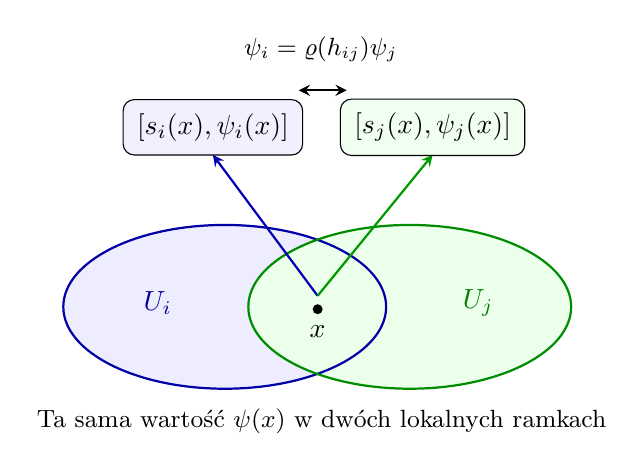
\begin{tikzpicture}[>=stealth,scale=1]
 \fill[blue!7] (-4.7,-1.1) ellipse (2.05 and 1.04);
 \fill[green!8] (-2.35,-1.1) ellipse (2.05 and 1.04);
 \draw[blue!65!black,thick] (-4.7,-1.1) ellipse (2.05 and 1.04);
 \draw[green!55!black,thick] (-2.35,-1.1) ellipse (2.05 and 1.04);
 \fill[black] (-3.52,-1.13) circle (1.8pt);
 \node[below] at (-3.52,-1.22) {$x$};
 \node[blue!60!black] at (-5.55,-1.05) {$U_i$};
 \node[green!50!black] at (-1.48,-1.05) {$U_j$};
 \draw[->,thick,blue!70!black] (-3.52,-.96)--(-4.85,.83);
 \draw[->,thick,green!60!black] (-3.52,-.96)--(-2.06,.83);
 \node[draw,rounded corners,fill=blue!6,align=center,inner sep=5pt]
  at (-4.85,1.18) {$[s_i(x),\psi_i(x)]$};
 \node[draw,rounded corners,fill=green!6,align=center,inner sep=5pt]
  at (-2.06,1.18) {$[s_j(x),\psi_j(x)]$};
 \draw[<->,thick] (-3.76,1.65)--(-3.15,1.65);
 \node[font=\small] at (-3.48,2.17)
  {$\psi_i=\varrho(h_{ij})\psi_j$};
 \node[font=\small] at (-3.47,-2.55)
  {Ta sama wartość $\psi(x)$ w dwóch lokalnych ramkach};
\end{tikzpicture}

{\small\itshape Dwie lokalne reprezentacje jednego pola spinorowego.
Warunek sklejania zapewnia zgodność na przecięciu obszarów.}
\end{center}

Różniczkowanie pól spinorowych wymaga koneksji na $S(M)$.
Uzasadnienie oraz prawo transformacji jej lokalnych form
podajemy w tomie II, w podsekcji
\hyperref[sec:koneksja-spinorowa-transformacja]{„Koneksja na wiązce spinorowej”}
rozdziału o koneksjach.


\par\smallskip
{\footnotesize\noindent\emph{Dalsza lektura:}
Rachunki z konwencją $v^2=-\|v\|^2$
można porównać z notatkami Briana Conrada,
\emph{Clifford algebras and spin groups},
\url{https://math.stanford.edu/~conrad/210CPage/handouts/clifford.pdf}.
Budowę struktur spinowych i opis przeszkody
$w_2$ rozwijają notatki Konstantina Wernliego,
\emph{Lecture Notes on Spin Geometry},
\url{https://arxiv.org/pdf/1911.09766}.
Obie lektury używają miejscami innej kolejności tematów.
Powyższy test znaków został dowiedziony bez użycia kohomologii;
jego interpretacja jako klasy w $H^2$ korzysta z teorii
kohomologii Čech, której tutaj nie dowodziliśmy.\par}
\clearpage

\chapter{Podstawy algebry abstrakcyjnej}
\label{ch:algebra-abstrakcyjna}

\providecommand{\atlasref}[2]{#2}
\index{algebra abstrakcyjna@Algebra abstrakcyjna}

Zbierzemy pojęcia grup, pierścieni i modułów potrzebne
do algebry homologicznej. Konstrukcje ilorazowe pozwalają
narzucać relacje, a iloczyn tensorowy pozwala zastąpić
odwzorowanie dwuliniowe liniowym. Wcześniejszy
Rozdział~\ref{ch:algebra-tensorowa} dotyczył przestrzeni
nad ciałem; tutaj pracujemy nad pierścieniem.
W Rozdziale~\ref{ch:grass-spin} wystąpił też moduł
algebry Clifforda; wrócimy do tego przykładu.

\section{Grupy, słowa i prezentacje}
\label{sec:grupy-prezentacje-5}
\index{grupa wolna@Grupa wolna}
\index{prezentacja grupy@Prezentacja grupy}

Zanim przejdziemy do modułów, zbierzmy język
potrzebny przy grupie podstawowej i
Twierdzeniu~\ref{thm:van-kampen}. Grupa opisuje
odwracalne składanie działań. W grupie klas
pętli opartych w jednym punkcie działaniem
jest składanie pętli, a odwrotność reprezentuje
pętla przebiegnięta w przeciwnym kierunku.

\subsection*{Grupy, homomorfizmy i ilorazy}

\begin{definicja}[Grupa i homomorfizm]
\index{grupa i homomorfizm@Grupa i homomorfizm}
\label{def:grupa-hom-5}
\emph{Grupa} $(G,\cdot,1)$ to zbiór z łącznym
mnożeniem, elementem neutralnym $1$ i
odwrotnością $g^{-1}$ każdego $g\in G$.
Nie zakładamy przemienności. Odwzorowanie
$\varphi:G\to H$ jest \emph{homomorfizmem},
jeśli $\varphi(gh)=\varphi(g)\varphi(h)$.
Wtedy $\varphi(1)=1$ i
$\varphi(g^{-1})=\varphi(g)^{-1}$.
Istotnie, $\varphi(1)^2=\varphi(1)$, więc skracanie daje
$\varphi(1)=1$; następnie stosujemy $\varphi$ do $gg^{-1}=1$.
Bijektywny homomorfizm nazywamy \emph{izomorfizmem}.
\end{definicja}

Przykładem jest $(\Z,+,0)$;
w zapisie addytywnym odwrotnością $m$
jest $-m$. Grupa permutacji trzech
elementów dostarcza przykładu
nieprzemiennego: przestawienia
$(12)(23)=(123)$ i $(23)(12)=(132)$ są różne
(permutacje składamy od prawej do lewej).

\begin{definicja}[Podgrupa normalna i iloraz]
\index{podgrupa normalna i iloraz@Podgrupa normalna i iloraz}
\label{def:normal-quotient-5}
\emph{Podgrupa} $N\leq G$ to podzbiór zawierający $1$
i zamknięty na mnożenie oraz branie odwrotności.
\emph{Warstwa lewostronna} to $gN=\{gn:n\in N\}$.
Mamy $gN=hN$ dokładnie wtedy, gdy $h^{-1}g\in N$:
z równości warstw wynika $g=hn$ dla pewnego $n\in N$,
a z $g=hn$ wynika $gN=hnN=hN$.
Podgrupa $N\leq G$ jest \emph{normalna},
gdy $gNg^{-1}=N$ dla każdego $g\in G$.
Wówczas zbiór warstw $G/N$ staje się
grupą przez $(gN)(hN)=ghN$.
Jądro homomorfizmu
$\ker\varphi=\{g:\varphi(g)=1\}$
jest normalne. \emph{Domknięcie normalne}
zbioru $R\subset G$, oznaczane
$\langle\!\langle R\rangle\!\rangle$,
jest najmniejszą podgrupą normalną
zawierającą $R$.
\end{definicja}

\begin{proof}[Dlaczego iloraz jest dobrze określony?]
Jeśli $g'=gn$ i $h'=hm$ dla $n,m\in N$,
to $g'h'=gnhm=gh(h^{-1}nh)m$.
Normalność daje $h^{-1}nh\in N$,
zatem $g'h'N=ghN$. Mnożenie
nie zależy więc od wybranych
reprezentantów. Łączność dziedziczymy z $G$;
elementem neutralnym jest $N$, a odwrotnością $gN$ jest $g^{-1}N$.
Dla jądra mamy $\varphi(1)=1$, a jeśli $x,y\in\ker\varphi$,
to $\varphi(xy^{-1})=\varphi(x)\varphi(y)^{-1}=1$;
jest więc podgrupą. Ponadto
$\varphi(gng^{-1})=
\varphi(g)1\varphi(g)^{-1}=1$.
Elementy domknięcia normalnego
są skończonymi iloczynami
sprzężeń $grg^{-1}$ i ich
odwrotności, $r\in R$:
zbiór tych iloczynów jest
podgrupą normalną zawierającą
$R$ i mieści się w każdej takiej
podgrupie.
\end{proof}

Normalność jest dokładnie warunkiem potrzebnym do mnożenia warstw.
Istotnie, gdyby iloczyn warstw był niezależny od reprezentantów,
to dla $n\in N$ mielibyśmy
$(gN)(nN)(g^{-1}N)=(gN)N(g^{-1}N)=N$,
czyli $gng^{-1}\in N$. Zmieniając $g$ na $g^{-1}$,
dostajemy równość $gNg^{-1}=N$.
Na przykład w $S_3$ podgrupa $N=\{1,(12)\}$ nie jest normalna:
$(23)(12)(23)=(13)\notin N$. Przy próbie obliczenia
$N\cdot(23)N$ wybór reprezentanta $1$ albo $(12)$ pierwszej
warstwy daje odpowiednio $(23)N$ i $(12)(23)N$.
Są to różne warstwy, bo $(23)^{-1}(12)(23)=(13)\notin N$.

\begin{stwierdzenie}[Twierdzenie o homomorfizmie grup]
\index{twierdzenie o homomorfizmie grup}
\label{prop:group-first-isomorphism-5}
Jeśli $\varphi:G\to H$ jest homomorfizmem i $N=\ker\varphi$,
to $\varphi$ wyznacza izomorfizm
\[
 \overline\varphi:G/N\longrightarrow\operatorname{im}\varphi,
 \qquad gN\longmapsto\varphi(g).
\]
\end{stwierdzenie}
\begin{proof}
Jądro $N$ jest normalne, więc $G/N$ jest grupą. Jeśli $gN=hN$,
to $h^{-1}g\in N$, skąd
$\varphi(h)^{-1}\varphi(g)=\varphi(h^{-1}g)=1$.
Wzór na $\overline\varphi$ nie zależy zatem od reprezentanta.
Ponadto
$\overline\varphi((gN)(hN))=\varphi(gh)
=\varphi(g)\varphi(h)$, więc jest homomorfizmem.
Jego obrazem jest z definicji $\operatorname{im}\varphi$.
Jeśli $\overline\varphi(gN)=\overline\varphi(hN)$, to
$\varphi(h^{-1}g)=1$, czyli $h^{-1}g\in N$ i $gN=hN$.
Stąd $\overline\varphi$ jest iniektywne. Równoważnie, dwa
elementy $G$ mają ten sam obraz dokładnie wtedy, gdy należą
do tej samej warstwy jądra.
\end{proof}

\begin{przyklad}[Reszty modulo $m$]
\label{prz:Zmodm-grupa-5}
Niech $m\geq2$.
W grupie addytywnej $\Z$ każda
podgrupa jest normalna.
Iloraz $\Z/m\Z$ ma elementy
$[0],\ldots,[m-1]$ i dodawanie
$[a]+[b]=[a+b]$. Homomorfizm
$\Z\to\Z/m\Z$ ma jądro $m\Z$.
Na przykład w $\Z/5\Z$ mamy $[3]+[4]=[2]$, ponieważ
$3+4-2=5\in5\Z$. Twierdzenie~\ref{prop:group-first-isomorphism-5}
wyjaśnia, że iloraz utożsamia dokładnie liczby o tej samej
reszcie modulo $m$.
\end{przyklad}

\subsection*{Grupy wolne i iloczyn wolny}

\begin{definicja}[Grupa wolna i iloczyn wolny]
\index{grupa wolna i iloczyn wolny@Grupa wolna i iloczyn wolny}
\index{slowo w grupie wolnej@słowo w grupie wolnej}
\label{def:free-groups-5}
Niech $A$ będzie zbiorem \emph{symboli},
zwanych generatorami. Dla każdego $a\in A$
tworzymy nowy symbol $a^{-1}$;
zbiór tych nowych symboli oznaczamy $A^{-1}$
i przyjmujemy $(a^{-1})^{-1}=a$.
\emph{Słowo} w alfabecie
$A^{\pm1}=A\sqcup A^{-1}$ jest skończonym
ciągiem liter $x_1\cdots x_r$, $r\geq0$.
Długość słowa to $r$; jedyne słowo długości
zero oznaczamy $\varnothing$ i nazywamy pustym.
Słowa można sklejać, czyli konkatenować:
$(x_1\cdots x_r)(y_1\cdots y_s)
=x_1\cdots x_ry_1\cdots y_s$.

\emph{Redukcja elementarna} usuwa sąsiednie
litery $xx^{-1}$ lub $x^{-1}x$.
Słowo jest \emph{zredukowane}, gdy nie zawiera
takiej pary. Dwa słowa uznajemy za równoważne,
jeżeli można przejść od jednego do drugiego
skończonym ciągiem wstawień lub usunięć
takich par. \emph{Grupa wolna} $F(A)$
to zbiór tych klas, z mnożeniem zadanym
przez sklejanie słów.

Dla grup $G,H$ \emph{iloczyn wolny} $G*H$
powstaje ze słów w \emph{rozłącznej sumie} alfabetów
$(G\setminus\{1_G\})\sqcup(H\setminus\{1_H\})$.
Litera pamięta swój czynnik, nawet gdy $G=H$.
Redukcja zastępuje sąsiednie litery jednego czynnika
ich iloczynem w tym czynniku; jeśli iloczyn jest jedynką,
usuwa obie litery. Równoważność słów dopuszcza zarówno
te redukcje, jak i operacje odwrotne.
$G*H$ jest zbiorem klas z mnożeniem przez konkatenację.
Słowo zredukowane ma litery z obu czynników naprzemiennie.
\end{definicja}

Zanim utożsamimy klasy ze słowami zredukowanymi,
trzeba wiedzieć, że wynik redukcji nie zależy
od kolejności kasowania par. Sam zbiór
\emph{wszystkich} słów z konkatenacją
jest tylko monoidem: słowa $aa^{-1}$
i $\varnothing$ nie są w nim dosłownie równe.

\begin{stwierdzenie}[Jednoznaczna postać zredukowana]
\index{redukcja slowa@redukcja słowa}
\label{prop:free-reduction-5}
Każda klasa w $F(A)$ zawiera dokładnie jedno
słowo zredukowane. Jeżeli $\operatorname{red}(w)$
oznacza to słowo, działanie grupowe ma postać
\[
 u\cdot v=\operatorname{red}(uv),\qquad
 1=\varnothing,\qquad
 (x_1\cdots x_r)^{-1}=x_r^{-1}\cdots x_1^{-1}.
\]
\end{stwierdzenie}
\begin{proof}
Czytamy słowo od lewej do prawej i trzymamy
\emph{stos} już przeczytanych liter.
Gdy następna litera jest odwrotnością
litery na wierzchu stosu, zdejmujemy wierzch;
w przeciwnym razie dokładamy nową literę.
Po ostatnim kroku na stosie nie ma sąsiedniej
pary odwrotnej, więc otrzymaliśmy słowo
zredukowane. Po każdym kroku stos reprezentuje tę samą
klasę co przeczytany fragment: dopisujemy literę albo
usuwamy końcową parę odwrotną. Wynik należy więc do klasy
początkowego słowa.

Sprawdźmy niezależność od usuwania par.
Operacja dopisania litery $x$ do słowa
na stosie jest odwracalna: operacja
dopisania $x^{-1}$ cofa ją, zarówno gdy
pierwszy krok dołożył literę, jak i wtedy,
gdy ją skasował. Dlatego przeczytanie
fragmentu $xx^{-1}$ nie zmienia stanu stosu.
Usunięcie takiego fragmentu z dowolnego miejsca
słowa nie zmienia końcowego wyniku algorytmu.
Każde słowo równoważne daje zatem ten sam wynik.
Jeśli słowo jest już zredukowane, algorytm
pozostawia je bez zmian; w każdej klasie
może więc być tylko jedno takie słowo.

Sklejanie jest łączne przed redukcją, a
usuwanie par nie zmienia wyniku algorytmu.
Stąd $\operatorname{red}(\operatorname{red}(uv)w)
=\operatorname{red}(uvw)
=\operatorname{red}(u\operatorname{red}(vw))$.
Słowo puste jest jedynką. Zapisane w tezie
słowo odwrotne po sklejeniu z oryginałem
redukuje się kolejno od środka do słowa pustego.
To sprawdza wszystkie aksjomaty grupy.
\end{proof}

\begin{przyklad}[Słowa i działanie na słowach]
\label{prz:redukcja-slow-5}
W $F(\{a,b\})$ słowo
$ab\,b^{-1}a^{-1}ba$
redukujemy najpierw do
$aa^{-1}ba$, a następnie
do $ba$. Słowa $ab$ i $ba$
są już zredukowane i różne,
więc grupa ta nie jest przemienna.
Dla jednego generatora każde słowo
redukuje się do $a^m$ z jednoznacznym
$m\in\Z$; stąd $F(\{a\})\cong\Z$.

Grupa $F(A)$ działa na zbiorze zredukowanych
słów przez mnożenie z lewej:
$u\cdot w=\operatorname{red}(uw)$.
Na przykład $a\cdot(a^{-1}b)=b$.
Jest to działanie, bo łączność udowodniono
powyżej; odwrotna operacja do działania
przez $a$ to działanie przez $a^{-1}$.
Jest ono przechodnie, gdyż $w\cdot\varnothing=w$,
i wolne: jeśli $u\cdot w=w$, to w grupie
$uw=w$, zatem po pomnożeniu przez $w^{-1}$
dostajemy $u=1$. Ten sam zbiór ma również
działanie z prawej $w\cdot u=\operatorname{red}(wu)$.
Rysunek~\ref{fig:free-words-5} pokazuje
pojedyncze kroki tego drugiego działania.
Na przykład iloczyn dwóch zredukowanych słów
$ab$ i $b^{-1}a$ trzeba jeszcze skrócić:
$\operatorname{red}(ab\,b^{-1}a)=a^2$.
Każde słowo zredukowane wyznacza drogę od $1$ bez natychmiastowego
powrotu po przebytej krawędzi. Jednoznaczność postaci zredukowanej
oznacza, że takie drogi nie tworzą cykli: pełny graf jest drzewem,
a Rysunek~\ref{fig:free-words-5} pokazuje tylko jego fragment.
Istotnie, cykl prosty można przez mnożenie z lewej przenieść tak,
aby zaczynał się w $1$. Litery kolejnych krawędzi dałyby wtedy
niepuste słowo zredukowane reprezentujące jedynkę, wbrew
Stwierdzeniu~\ref{prop:free-reduction-5}.
\end{przyklad}

\begin{figure}[htbp]
\centering
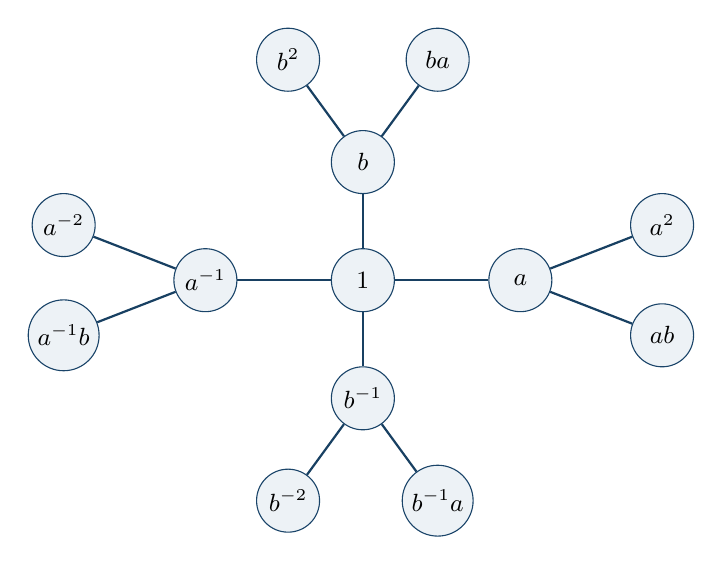
\begin{tikzpicture}[>=Latex,font=\small,
 every node/.style={circle,draw=manifoldblue!75!black,
 fill=manifoldblue!8,inner sep=2pt,minimum size=8mm}]
 \node (e) at (0,0) {$1$};
 \node (a) at (2,0) {$a$};
 \node (ai) at (-2,0) {$a^{-1}$};
 \node (b) at (0,1.5) {$b$};
 \node (bi) at (0,-1.5) {$b^{-1}$};
 \node (aa) at (3.8,.7) {$a^2$};
 \node (ab) at (3.8,-.7) {$ab$};
 \node (aiai) at (-3.8,.7) {$a^{-2}$};
 \node (aib) at (-3.8,-.7) {$a^{-1}b$};
 \node (bb) at (-.95,2.8) {$b^2$};
 \node (ba) at (.95,2.8) {$ba$};
 \node (bibi) at (-.95,-2.8) {$b^{-2}$};
 \node (bia) at (.95,-2.8) {$b^{-1}a$};
 \foreach \x/\y in {e/a,e/ai,e/b,e/bi,a/aa,a/ab,
 ai/aiai,ai/aib,b/bb,b/ba,bi/bibi,bi/bia}
   \draw[thick,manifoldblue!70!black] (\x)--(\y);
\end{tikzpicture}
\caption{Fragment grafu słów zredukowanych w
$F(\{a,b\})$. Krawędź oznacza dopisanie
z prawej jednej litery $a^{\pm1}$ albo $b^{\pm1}$
i ewentualną redukcję. Powrót po krawędzi
odpowiada dopisaniu litery odwrotnej.}
\label{fig:free-words-5}
\end{figure}

\begin{stwierdzenie}[Własność uniwersalna grupy wolnej]
\label{prop:free-universal-5}
Dla dowolnej grupy $K$ i dowolnego wyboru
elementów $h_a\in K$, $a\in A$, istnieje
dokładnie jeden homomorfizm $\Phi:F(A)\to K$
spełniający $\Phi(a)=h_a$.
\end{stwierdzenie}
\begin{proof}
Na słowach musi on mieć postać
\[
 \Phi(a_1^{\epsilon_1}\cdots a_r^{\epsilon_r})
 =h_{a_1}^{\epsilon_1}\cdots h_{a_r}^{\epsilon_r},
 \qquad \epsilon_i\in\{1,-1\}.
\]
Usunięcie sąsiedniej pary odwrotnej nie zmienia
iloczynu po prawej. Wzór zależy więc tylko
od klasy słowa i jest dobrze określony.
Sklejanie słów odpowiada mnożeniu obrazów,
zatem $\Phi$ jest homomorfizmem.
Każde słowo jest iloczynem generatorów
i ich odwrotności, co dowodzi jednoznaczności.
Właśnie brak dodatkowych relacji między
generatorami nazywamy \emph{wolnością}.
\end{proof}

\begin{stwierdzenie}[Postać normalna i własność uniwersalna iloczynu wolnego]
\label{prop:free-product-normal-5}
Każdy element $G*H$ ma dokładnie jeden zapis jako słowo
naprzemienne o literach różnych od jedynki, z dopuszczeniem
słowa pustego. Odwzorowania $G\to G*H$ i $H\to G*H$,
wysyłające element niejednostkowy na słowo jednoliterowe,
a jedynkę na słowo puste, są iniektywnymi homomorfizmami.
Dla każdej pary homomorfizmów $f:G\to K$, $h:H\to K$
istnieje dokładnie jeden homomorfizm $\Phi:G*H\to K$
ograniczający się na czynnikach do $f$ oraz $h$.
\end{stwierdzenie}
\begin{proof}
Czytamy litery po kolei i przechowujemy stos liter
niejednostkowych, pochodzących naprzemiennie z obu czynników.
Dla $x$ z jednego czynnika oznaczmy przez $T_x$ operację
dopisania $x$: literę z innego czynnika dokładamy, a z tego
samego mnożymy z ostatnią literą stosu. Gdy iloczyn jest
jedynką, zdejmujemy tę ostatnią literę. Przyjmujemy $T_1=\id$.
Każdy krok jest dozwoloną redukcją, więc wynik algorytmu
należy do klasy czytanego słowa.

Kluczowa jest równość $T_y(T_x(u))=T_{xy}(u)$, gdy $x,y$
pochodzą z tego samego czynnika. Jeśli któraś litera jest
jedynką, równość jest natychmiastowa. W pozostałym przypadku:
\begin{itemize}[leftmargin=*]
\item Gdy $u$ jest pusty albo kończy się literą drugiego
czynnika, najpierw dopisujemy $x$, potem zastępujemy $xy$
jedną literą albo usuwamy je, jeśli $xy=1$. To właśnie $T_{xy}(u)$.
\item Gdy $u=vz$ i $z$ jest z tego samego czynnika co $x,y$,
słowo $v$ jest puste albo kończy się w drugim czynniku.
Jeśli $zx\ne1$, dwa kroki zastępują końcówkę przez
$(zx)y=z(xy)$, z usunięciem jedynki. Dla $xy=1$ odzyskujemy $vz$;
dla $xy\ne1$ jest to pojedynczy krok $T_{xy}$.
Jeśli $zx=1$, pierwszy krok usuwa $z$, a drugi daje $vy$.
Z kolei $z(xy)=y$; gdy $xy\ne1$, pojedynczy krok również daje $vy$.
Gdy $xy=1$, mamy $y=z$, więc $vy=u=T_1(u)$.
\end{itemize}
Zastąpienie sąsiednich liter ich iloczynem nie zmienia zatem
stosu po przeczytaniu tego fragmentu, ani wyniku po przeczytaniu
reszty słowa. Dotyczy to także odwrotnej operacji.
Wynik jest stały na klasie równoważności. Ponieważ algorytm
pozostawia słowo naprzemienne bez zmian, w każdej klasie jest
dokładnie jedno takie słowo.

Relacje można wykonywać wewnątrz dowolnego dłuższego słowa,
więc konkatenacja jest dobrze określona na klasach i łączna.
Słowo puste jest jedynką, a odwrócenie kolejności liter
i zastąpienie ich odwrotnościami daje odwrotność słowa.
Relacje wewnątrz czynników zapewniają, że ich odwzorowania
do $G*H$ są homomorfizmami. Jednoznaczność postaci normalnej
daje ich iniektywność; obrazy czynników mają tylko jedynkę wspólną.

Definiujemy $\Phi(x_1\cdots x_r)$ jako iloczyn obrazów liter,
używając $f$ lub $h$ zależnie od czynnika.
Redukcja w jednym czynniku nie zmienia tego iloczynu, bo
$f$ i $h$ są homomorfizmami. Wzór przechodzi więc na klasy.
Konkatenacja słów odpowiada mnożeniu obrazów, a każdy element
jest iloczynem liter z czynników; daje to istnienie i jednoznaczność $\Phi$.
\end{proof}

Ta własność uniwersalna będzie używana w
Twierdzeniu~\ref{thm:van-kampen}.

Na przykład dla $G=\langle a\rangle\cong\Z$
i $H=\langle b\rangle\cong\Z$ własności
uniwersalne dają $G*H\cong F(\{a,b\})$.
Iloczyn słów naprzemiennych
$(ab)(b^{-1}a)$ redukuje się do $a^2$:
po skasowaniu $bb^{-1}$ zostaje $aa$.
Podobnie, dla $G=\{1,s\}$ z $s^2=1$ i
$H=\{1,t,t^2\}$ z $t^3=1$ mamy w $G*H$ redukcję
\[
 (st^2)(ts)=s(t^2t)s=s\,1\,s=s^2=1.
\]
Pierwsze skrócenie odbywa się w $H$, a ostatnie w $G$;
oba są konieczne, by otrzymać postać normalną.

Nie należy mylić iloczynu wolnego z iloczynem prostym.
Dla $G=\langle a\mid a^2=1\rangle$ i
$H=\langle b\mid b^2=1\rangle$, obu rzędu dwa,
słowa $(ab)^k$, $k\geq0$, są różnymi postaciami normalnymi.
Zatem $G*H$ jest nieskończony, podczas gdy $G\times H$ ma
cztery elementy. W $G*H$ nie narzucamy przemienności liter
z różnych czynników.

\subsection*{Generatory i relacje}

\begin{definicja}[Prezentacja grupy]
\index{prezentacja grupy@Prezentacja grupy}
\label{def:prezentacja-grupy-5}
Jeśli $R$ jest zbiorem słów
w $F(A)$, to
\[
 \langle A\mid R\rangle
 :=F(A)/\langle\!\langle R\rangle\!\rangle
\]
nazywamy \emph{grupą o generatorach}
$A$ i \emph{relacjach} $R$.
Relacja $r=1$ oznacza, że jej
wszystkie konsekwencje po
mnożeniu i sprzęganiu również
stają się jedynką.
\end{definicja}

\begin{stwierdzenie}[Odwzorowanie zadane na generatorach i relacjach]
\label{prop:presentation-universal-5}
Niech $K$ będzie grupą. Wybór elementów $h_a\in K$ dla $a\in A$
wyznacza homomorfizm $\langle A\mid R\rangle\to K$ wysyłający
klasę $a$ na $h_a$ wtedy i tylko wtedy, gdy każde słowo $r\in R$
po podstawieniu $a\mapsto h_a$ daje jedynkę w $K$.
Jeśli taki homomorfizm istnieje, jest jedyny.
\end{stwierdzenie}
\begin{proof}
Z własności uniwersalnej grupy wolnej
(Stwierdzenie~\ref{prop:free-universal-5}) otrzymujemy jedyny
homomorfizm $f:F(A)\to K$ o zadanych obrazach generatorów.
Jeśli $f(r)=1$ dla wszystkich $r\in R$, normalność jądra
implikuje $\langle\!\langle R\rangle\!\rangle\subseteq\ker f$.
Możemy więc określić
$\bar f(w\langle\!\langle R\rangle\!\rangle)=f(w)$.
Gdy dwie warstwy są równe, ich reprezentanci różnią się elementem
jądra $f$, zatem wzór jest dobrze określony; zachowuje też iloczyn.
Odwrotnie, homomorfizm z ilorazu wysyła każdą klasę $r\in R$
na jedynkę, więc podstawione słowo musi być jedynką.
Jednoznaczność wynika z tego, że klasy liter $a$ generują iloraz.
\end{proof}

\begin{przyklad}[Jedna relacja potęgowa]
\label{prz:cyclic-presentation-5}
Dla $m\geq2$ grupa $\langle a\mid a^m\rangle$ jest izomorficzna
z $\Z/m\Z$. Każde jej słowo jest potęgą $a^k$;
relacja $a^m=1$ pozwala zmniejszyć wykładnik modulo $m$.
Nie powoduje ona dalszych utożsamień: przypisanie
$a\mapsto[1]\in\Z/m\Z$ respektuje $a^m=1$ i daje homomorfizm
z prezentacji na $\Z/m\Z$. Obrazy $1,a,\ldots,a^{m-1}$ są różne,
więc te $m$ potęg są różnymi elementami grupy.
\end{przyklad}

\begin{przyklad}[Prezentacja grupy torusa]
\label{prz:prezentacja-torusa-5}
Niech $F(\{a,b\})$ będzie grupą wolną
na dwóch symbolach. Relacja
$aba^{-1}b^{-1}=1$
jest równoważna $ab=ba$.
Samo słowo $aba^{-1}b^{-1}$ jest zredukowane i niepuste
w $F(\{a,b\})$; staje się jedynką dopiero po przejściu do ilorazu.
Po jej narzuceniu każde słowo
można przestawić do postaci
$a^m b^n$, $m,n\in\Z$.
Odwzorowanie
$F(\{a,b\})\to\Z^2$ dane przez
$a\mapsto(1,0)$,
$b\mapsto(0,1)$
zabija tę relację i wysyła
$a^m b^n$ na $(m,n)$.
Postacie te są więc wzajemnie
różne, a zatem
\[
 \langle a,b\mid aba^{-1}b^{-1}\rangle
 \cong\Z^2.
\]
Sklejenie przeciwnych boków kwadratu
tworzy torus. Brzeg kwadratu przed
sklejeniem odczytujemy przeciwnie do ruchu wskazówek zegara
jako słowo $aba^{-1}b^{-1}$; orientacje boków
pokazuje Rysunek~\ref{fig:torus-square-5}.
Topologiczne uzasadnienie, że
prezentacja opisuje $\pi_1(T^2)$,
podamy przy
Twierdzeniu~\ref{thm:van-kampen}.
\end{przyklad}

\begin{figure}[htbp]
\centering
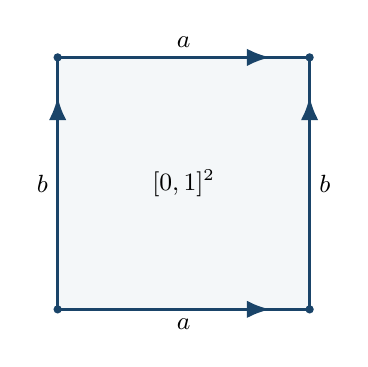
\begin{tikzpicture}[>=Latex,font=\small]
 \fill[manifoldblue!5] (0,0) rectangle (3.2,3.2);
 \draw[very thick,manifoldblue!75!black] (0,0) rectangle (3.2,3.2);
 \draw[->,very thick,manifoldblue!75!black] (.5,0)--(2.7,0);
 \draw[->,very thick,manifoldblue!75!black] (.5,3.2)--(2.7,3.2);
 \draw[->,very thick,manifoldblue!75!black] (0,.5)--(0,2.7);
 \draw[->,very thick,manifoldblue!75!black] (3.2,.5)--(3.2,2.7);
 \node[below] at (1.6,0) {$a$};
 \node[above] at (1.6,3.2) {$a$};
 \node[left] at (0,1.6) {$b$};
 \node[right] at (3.2,1.6) {$b$};
 \foreach \x/\y in {0/0,3.2/0,3.2/3.2,0/3.2}
   \fill[manifoldblue!75!black] (\x,\y) circle (1.5pt);
 \node at (1.6,1.6) {$[0,1]^2$};
\end{tikzpicture}
\caption{Kwadrat fundamentalny torusa. Strzałki wskazują
orientacje identyfikowanych par boków. Obchodząc brzeg kwadratu
od lewego dolnego wierzchołka przeciwnie do ruchu wskazówek zegara,
czytamy $a,b,a^{-1},b^{-1}$; wszystkie cztery wierzchołki
po sklejeniu reprezentują ten sam punkt.}
\label{fig:torus-square-5}
\end{figure}


\subsection*{Iloczyn prosty grup}
\index{iloczyn prosty grup}
\index{grupa!iloczyn prosty}

Iloczyn prosty opisuje niezależne wykonywanie dwóch działań.
\begin{definicja}[Iloczyn prosty]
Dla grup $G,H$ ich \emph{iloczyn prosty} jest zbiorem $G\times H$
z mnożeniem $(g_1,h_1)(g_2,h_2)=(g_1g_2,h_1h_2)$.
Jedynką jest $(e_G,e_H)$, a $(g,h)^{-1}=(g^{-1},h^{-1})$.
Łączność wynika z łączności w każdej współrzędnej.
\end{definicja}

Inkluzje $g\mapsto(g,e_H)$ i $h\mapsto(e_G,h)$ są homomorfizmami.
Ich obrazy są normalne: sprzęganie odbywa się współrzędnie.
Elementy z różnych czynników komutują i każdy element ma jednoznaczny
rozkład $(g,h)=(g,e_H)(e_G,h)$.

\begin{stwierdzenie}[Wewnętrzny iloczyn prosty]
Jeśli $G,H$ są normalnymi podgrupami $K$, $G\cap H=\{e\}$ i $K=GH$,
to $F:G\times H\to K$, $F(g,h)=gh$, jest izomorfizmem.
Zapis $GH$ oznacza zbiór wszystkich iloczynów $gh$.
\end{stwierdzenie}
\begin{proof}
Komutator $ghg^{-1}h^{-1}$ należy do $G$ i do $H$ przez normalność:
jest iloczynem $g(hg^{-1}h^{-1})$ elementów $G$ oraz
iloczynem $(ghg^{-1})h^{-1}$ elementów $H$,
więc jest jedynką. Dlatego $gh=hg$ i
\[
 F(g_1g_2,h_1h_2)=g_1g_2h_1h_2=g_1h_1g_2h_2
 =F(g_1,h_1)F(g_2,h_2).
\]
Warunek $K=GH$ daje surjektywność. Jeśli $F(g,h)=e$, to
$g=h^{-1}\in G\cap H$, zatem $g=h=e$; jądro jest trywialne.
\end{proof}

\begin{przyklad}[Grupy cykliczne i grupa Kleina]
Grupę generowaną przez jeden element nazywamy \emph{cykliczną}.
Piszemy $C_m=\Z/m\Z$ dla $m\geq1$. Rząd elementu jest najmniejszą
dodatnią liczbą potęg dającą jedynkę, o ile taka liczba istnieje.
W $C_m\times C_n$ element $([1],[1])$ ma rząd
$\operatorname{lcm}(m,n)$: jego $j$-krotność znika dokładnie wtedy,
gdy $m\mid j$ i $n\mid j$. Dla $\gcd(m,n)=1$ rząd wynosi $mn$,
więc ten element generuje całą grupę i $C_m\times C_n\cong C_{mn}$.
Na przykład $C_2\times C_3\cong C_6$. Natomiast w
$V_4:=C_2\times C_2$, zwanej \emph{grupą Kleina}, każdy niezerowy
element ma rząd dwa, więc nie ma generatora całej czteroelementowej grupy.
\end{przyklad}

\subsection*{Iloczyn półprosty grup}
\index{iloczyn półprosty grup}
\index{grupa!iloczyn półprosty}
\index{działanie grupy!przez automorfizmy}

Teraz jedna grupa może zmieniać sposób działania drugiej.
\emph{Automorfizmem} grupy $N$ nazywamy izomorfizm $N\to N$;
ich grupa ze składaniem to $\operatorname{Aut}(N)$.
Działanie $H$ na $N$ przez automorfizmy jest homomorfizmem
$\varphi:H\to\operatorname{Aut}(N)$, a więc
$\varphi(h_1h_2)=\varphi(h_1)\circ\varphi(h_2)$.

\begin{definicja}[Iloczyn półprosty]
\emph{Iloczyn półprosty} $N\rtimes_\varphi H$ ma zbiór elementów
$N\times H$ i mnożenie
\[
 (n_1,h_1)(n_2,h_2)
 =\bigl(n_1\varphi(h_1)(n_2),h_1h_2\bigr).
\]
Gdy działanie jest ustalone, skracamy zapis do $N\rtimes H$.
\end{definicja}

Sprawdźmy łączność. Pierwsza współrzędna obu sposobów mnożenia
trzech elementów jest równa
\[
 n_1\varphi(h_1)(n_2)\varphi(h_1h_2)(n_3)
 =n_1\varphi(h_1)\bigl(n_2\varphi(h_2)(n_3)\bigr).
\]
Druga to $h_1h_2h_3$. Jedynką jest $(e_N,e_H)$, a odwrotność
ma postać $(n,h)^{-1}=\bigl(\varphi(h^{-1})(n^{-1}),h^{-1}\bigr)$.
Wyznaczmy ją z równania $(n,h)(a,k)=(e_N,e_H)$:
druga współrzędna daje $k=h^{-1}$, a pierwsza
$\varphi(h)(a)=n^{-1}$, czyli $a=\varphi(h^{-1})(n^{-1})$.
Ten wybór działa z obu stron. Pierwsze współrzędne obu iloczynów to
\[
 \begin{aligned}
 n\,\varphi(h)\bigl(\varphi(h^{-1})(n^{-1})\bigr)
 &=nn^{-1}=e_N,\\
 \varphi(h^{-1})(n^{-1})\,\varphi(h^{-1})(n)
 &=\varphi(h^{-1})(n^{-1}n)=e_N.
 \end{aligned}
\]
Drugie współrzędne wynoszą odpowiednio $hh^{-1}=e_H$ i $h^{-1}h=e_H$.
Inkluzje $n\mapsto(n,e_H)$ i $h\mapsto(e_N,h)$ są homomorfizmami.
Pierwszy obraz jest normalny jako jądro homomorfizmu
$(n,h)\mapsto h$. Drugi nie musi być normalny, a wzór
\[
 (e_N,h)(n,e_H)(e_N,h)^{-1}=(\varphi(h)(n),e_H)
\]
pokazuje, że zadane działanie realizuje się przez sprzężenie.
Dla działania trywialnego, $\varphi(h)=\id_N$, odzyskujemy iloczyn prosty.

\begin{stwierdzenie}[Wewnętrzny iloczyn półprosty]
\index{iloczyn półprosty grup!wewnętrzny}
Niech $N,H\leq G$, $N\trianglelefteq G$, $N\cap H=\{e\}$ i $G=NH$.
Wtedy $G\cong N\rtimes H$, z działaniem $\varphi(h)(n)=hnh^{-1}$.
\end{stwierdzenie}
\begin{proof}
Normalność zapewnia, że sprzężenie przez $h$ jest automorfizmem $N$,
a składanie sprzężeń daje homomorfizm $\varphi$.
Dla $F(n,h)=nh$ mamy
\[
 F\bigl(n_1(h_1n_2h_1^{-1}),h_1h_2\bigr)
 =n_1h_1n_2h_2=F(n_1,h_1)F(n_2,h_2).
\]
Surjektywność wynika z $G=NH$, a $nh=e$ wymusza
$n=h^{-1}\in N\cap H=\{e\}$, więc $F$ jest iniektywny.
\end{proof}

\begin{uwaga}[Rozszczepiony ciąg dokładny]
\index{ciąg dokładny!rozszczepiony}
\index{rozszerzenie grup!rozszczepione}
Zapis $1\to N\xrightarrow{i}G\xrightarrow{p}H\to1$ oznacza,
że $i$ jest iniekcją, $p$ surjekcją i $i(N)=\ker p$; to
\emph{krótki ciąg dokładny grup}, czyli rozszerzenie $H$ przez $N$.
Jest \emph{rozszczepiony}, gdy istnieje homomorfizm $s:H\to G$
z $p\circ s=\id_H$. Dla iloczynu półprostego są to
$i(n)=(n,e_H)$, $p(n,h)=h$ i $s(h)=(e_N,h)$.
Odwrotnie, w rozszczepionym ciągu $s$ jest iniektywny,
$i(N)\cap s(H)=\{e\}$ i każdy $g\in G$ ma rozkład
$g=(g\,s(p(g))^{-1})s(p(g))$, z pierwszym czynnikiem w $\ker p$.
Poprzednie stwierdzenie daje zatem $G\cong N\rtimes H$.
\end{uwaga}

\begin{przyklad}[Grupa diedralna]
\index{grupa diedralna!jako iloczyn półprosty}
Dla $n\geq3$ niech $r$ będzie obrotem foremnego $n$-kąta o $2\pi/n$,
a $s$ jego odbiciem. Mamy $r^n=s^2=e$ i $srs^{-1}=r^{-1}$.
Ostatnią relację można zobaczyć we współrzędnych zespolonych:
wybieramy środek wielokąta w $0$ i oś odbicia jako oś rzeczywistą.
Wtedy $r(z)=\zeta z$ dla $\zeta=e^{2\pi i/n}$,
$s(z)=\overline z=s^{-1}(z)$ i
$(s\circ r\circ s^{-1})(z)=\overline{\zeta\overline z}
=\overline\zeta z=\zeta^{-1}z=r^{-1}(z)$.
Każda symetria ma postać $r^j$ lub $r^js$, $0\leq j<n$:
jej obraz jednego wierzchołka i wybór kierunku do sąsiedniego
wyznaczają całą symetrię. Te $2n$ możliwości są różne.
Grupa symetrii $D_n$ jest więc $C_n\rtimes C_2$, gdzie nietrywialny
element $C_2$ odwraca generator $C_n$. Dla trójkąta wszystkie
permutacje trzech wierzchołków są symetriami, stąd
$S_3\cong C_3\rtimes C_2$.
Na przykład w $D_5$ wzór $sr^js^{-1}=r^{-j}$ daje
$(r^2s)(r^3s)=r^2(sr^3s)=r^{-1}$; iloczyn dwóch odbić jest obrotem.
\end{przyklad}

\begin{przyklad}[Grupa afiniczna]
\index{grupa afiniczna!jako iloczyn półprosty}
Grupa odwracalnych macierzy rzeczywistych $\mathrm{GL}(n,\R)$
działa na addytywnej grupie $\R^n$ przez $A\cdot v=Av$.
Grupa odwracalnych odwzorowań afinicznych $x\mapsto Ax+v$ to
$\operatorname{Aff}(n)=\R^n\rtimes\mathrm{GL}(n,\R)$, ponieważ
\[
 A(Bx+w)+v=ABx+(v+Aw),\qquad
 (v,A)(w,B)=(v+Aw,AB).
\]
Macierz i przesunięcie są jednoznaczne: $v$ jest obrazem zera,
a $A$ jest częścią liniową. Czynnik $Aw$ odróżnia ten iloczyn
od iloczynu prostego.
\end{przyklad}

\begin{przyklad}[Ruchy euklidesowe]
\index{grupa euklidesowa!jako iloczyn półprosty}
\index{grupa ruchów euklidesowych}
Niech $\mathrm O(n)=\{A:A^TA=I\}$ i
$\mathrm{SO}(n)=\{A\in\mathrm O(n):\det A=1\}$.
Grupa izometrii przestrzeni euklidesowej to
$E(n)=\R^n\rtimes\mathrm O(n)$, z tym samym prawem składania.
Istotnie, dla izometrii $f$ połóżmy $v=f(0)$ i $g(x)=f(x)-v$.
Mamy $g(0)=0$ i $\|g(x)-g(y)\|=\|x-y\|$. Zatem
$\|g(x)\|=\|x\|$, a tożsamość polaryzacyjna
$2\langle u,w\rangle=\|u\|^2+\|w\|^2-\|u-w\|^2$ daje
$\langle g(x),g(y)\rangle=\langle x,y\rangle$.
Wektory $g(e_i)$ tworzą bazę ortonormalną, a współrzędne $g(x)$
w tej bazie wynoszą $\langle g(x),g(e_i)\rangle=x_i$.
Zatem $g(x)=\sum_i x_i g(e_i)=Ax$ z $A\in\mathrm O(n)$.
Odwrotnie, każde $Ax+v$ z taką macierzą zachowuje odległości.
Izometrie zachowujące orientację tworzą
$E^+(n)=\R^n\rtimes\mathrm{SO}(n)$.
Przykłady grup ortogonalnych oraz ich pokryć
przez grupy Pin i Spin omówiliśmy w
Rozdziale~\ref{ch:grass-spin}; jest to bezpośrednie
zastosowanie grup macierzowych w geometrii.
\end{przyklad}

\begin{uwaga}[Kolejność czynników i wybór działania]
W zapisie $N\rtimes H$ (również $H\ltimes N$) normalny jest czynnik
$N$, a $H$ działa na nim przez automorfizmy. Same grupy $N,H$ nie
wyznaczają wyniku: dla $C_3,C_2$ działanie trywialne daje abelową
grupę $C_6$, a odwracanie generatora daje nieabelową $S_3$.
Dlatego przy nieustalonym działaniu zachowujemy zapis $N\rtimes_\varphi H$.
\end{uwaga}


\section{Pierścienie, ideały i ilorazy}
\label{sec:pierscienie-idealy}
\index{pierscien@Pierścień}
\index{ideal@Ideał}

W grupie normalność podgrupy pozwala utworzyć
iloraz. Dla pierścieni podobną rolę pełni ideał:
trzeba zachować nie tylko dodawanie, lecz także
mnożenie klas przez dowolne elementy pierścienia.
W praktyce ideał jest zbiorem wyrażeń, które chcemy
uznać za zero. W ilorazie dwa elementy są równe
właśnie wtedy, gdy ich różnica należy do tego zbioru.

\begin{definicja}[Pierścień przemienny i homomorfizm]
\label{def:pierscien-przemienny}
\emph{Pierścień przemienny z jedynką} $R$ ma
dwa działania $+$ i mnożenie. Grupa $(R,+,0)$
jest abelowa, mnożenie jest łączne i przemienne,
ma jedynkę $1$, a rozdzielność
$r(s+t)=rs+rt$ wiąże oba działania.
Pierścień zerowy z $1=0$ jest dozwolony.
\emph{Homomorfizm pierścieni}
$\varphi:R\to S$ zachowuje dodawanie, mnożenie
i jedynkę: $\varphi(1_R)=1_S$.
\end{definicja}

Z przemienności mnożenia wynika też druga rozdzielność
$(r+s)t=rt+st$. Element $u\in R$ nazywamy
\emph{odwracalnym}, gdy istnieje $v\in R$ z $uv=1$;
zbiór takich elementów oznaczamy $R^\times$.
W każdym pierścieniu $0r=(0+0)r=0r+0r$,
zatem po dodaniu elementu przeciwnego $0r=0$.
Ponieważ $(r+(-r))s=0$, mamy także $(-r)s=-(rs)$.

Przykładami są $\Z$, $\Q$ i pierścień
wielomianów $\mathbb K[t]$ nad ciałem $\mathbb K$.
W $\Z$ nie każdy niezerowy element ma odwrotność
mnożeniową: równanie $2x=1$ nie ma rozwiązania
w $\Z$. Definicja pierścienia, w odróżnieniu od definicji
ciała, nie wymaga takich odwrotności. Dokładnie
$\Z^\times=\{-1,1\}$, choć $\Z\setminus\{0\}$ zawiera wszystkie
niezerowe liczby całkowite.

\begin{definicja}[Dziedzina całkowitości i ciało]
\label{def:dziedzina-cialo-5}
\index{dziedzina całkowitości}
\index{ciało}
Niezerowy element $a$ pierścienia przemiennego jest \emph{dzielnikiem
zera}, jeśli $ab=0$ dla pewnego $b\ne0$. \emph{Dziedzina całkowitości}
to pierścień przemienny z $1\ne0$ bez dzielników zera, czyli
$ab=0$ wymusza $a=0$ lub $b=0$. Pozwala to skracać niezerowy czynnik:
z $ac=bc$ i $c\ne0$ wynika $(a-b)c=0$, więc $a=b$.
\emph{Ciało} jest pierścieniem przemiennym z $1\ne0$, w którym
każdy niezerowy element ma odwrotność mnożeniową.
\end{definicja}

Każde ciało jest dziedziną: z $ab=0$, $a\ne0$, po pomnożeniu
przez $a^{-1}$ dostajemy $b=0$. Dziedzina $\Z$ nie jest ciałem,
natomiast $\Q$ jest ciałem. Również $\mathbb K[t]$ nad ciałem
jest dziedziną, bo iloczyn niezerowych współczynników wiodących
jest niezerowy. Pierścień $\Z/6\Z$ nie jest dziedziną:
$[2][3]=[0]$, choć oba czynniki są niezerowe.
Nie wolno więc w nim skracać dowolnego niezerowego czynnika:
$[2][3]=[2][0]$, lecz $[3]\ne[0]$.

\begin{definicja}[Ideał i pierścień ilorazowy]
\label{def:ideal-iloraz}
\emph{Ideał} $I\subseteq R$ jest podgrupą
addytywną zamkniętą na mnożenie przez
elementy $R$: jeśli $r\in R$ i $x\in I$,
to $rx\in I$. Pierścień $R/I$ ma klasy
$[r]=r+I$ oraz działania
$[r]+[s]=[r+s]$, $[r][s]=[rs]$.
Klasy spełniają $[r]=[s]$ dokładnie wtedy, gdy
$r-s\in I$. Dla $a\in R$ zbiór
$(a):=aR=\{ar:r\in R\}$ jest \emph{ideałem głównym}
generowanym przez $a$.
\end{definicja}

\begin{proof}[Dlaczego iloraz jest dobrze określony?]
Jeżeli $r'=r+i$ i $s'=s+j$ dla $i,j\in I$,
to $r'+s'-(r+s)=i+j\in I$ oraz
$r's'-rs=rj+is+ij\in I$.
Dlatego wynik obu działań nie zależy od
wyboru przedstawicieli. Prawa łączności, przemienności
i rozdzielności dziedziczą się z $R$;
zerem jest $[0]$, jedynką $[1]$, a elementem
przeciwnym do $[r]$ jest $[-r]$.
Odwzorowanie ilorazowe $q:R\to R/I$, $q(r)=[r]$,
jest więc surjektywnym homomorfizmem o jądrze $I$.

Jądro dowolnego homomorfizmu $\varphi:R\to S$ jest ideałem:
z $\varphi(x)=\varphi(y)=0$ wynikają
$\varphi(x-y)=0$ i
$\varphi(rx)=\varphi(r)\varphi(x)=0$.
Gdy $I=R$, iloraz jest pierścieniem zerowym
z $[1]=[0]$.
\end{proof}

\begin{stwierdzenie}[Ideały pierścienia liczb całkowitych]
\label{prop:idealy-Z-5}
Każdy ideał $I\subseteq\Z$ ma postać $m\Z$ dla dokładnie
jednego $m\geq0$. Dla $m=0$ jest to ideał zerowy.
\end{stwierdzenie}
\begin{proof}
Jeżeli $I\ne\{0\}$, to razem z niezerowym $a$ zawiera $-a$,
więc zawiera liczbę dodatnią. Niech $m$ będzie najmniejszą taką
liczbą. Ponieważ $I$ jest zamknięty na mnożenie przez liczby
całkowite, $m\Z\subseteq I$. Dla dowolnego $a\in I$
dzielenie z resztą daje $a=qm+r$ z $0\leq r<m$.
Liczba $r=a-qm$ należy do $I$, więc z minimalności $m$
wynika $r=0$. Stąd $a\in m\Z$ i $I=m\Z$.
Najmniejszy dodatni element wyznacza $m$ jednoznacznie;
przypadek $I=\{0\}$ daje $m=0$.
\end{proof}

\begin{stwierdzenie}[Własność ilorazu pierścienia]
\label{prop:ring-quotient-universal-5}
Niech $I\subseteq R$ będzie ideałem i niech
$f:R\to S$ będzie homomorfizmem pierścieni.
Istnieje homomorfizm $\bar f:R/I\to S$ spełniający
$f=\bar f\circ q$ dokładnie wtedy, gdy $I\subseteq\ker f$.
Jeśli istnieje, jest jedyny i dany wzorem $\bar f([r])=f(r)$.
W szczególności
\[
 R/\ker f\cong\operatorname{im}f,
 \qquad [r]\longmapsto f(r).
\]
\end{stwierdzenie}
\begin{proof}
Jeżeli $f=\bar f\circ q$, to dla $i\in I$ mamy
$q(i)=[0]$, więc $f(i)=\bar f([0])=0$.
Odwrotnie, załóżmy $I\subseteq\ker f$. Z równości
$[r]=[s]$ wynika $r-s\in I$, a stąd
$f(r)-f(s)=f(r-s)=0$. Wzór na $\bar f$ jest więc
dobrze określony. Zachowuje dodawanie, mnożenie i jedynkę,
ponieważ robi to $f$; warunek $f=\bar f\circ q$ zachodzi
dla każdego $r\in R$. Surjektywność $q$ wymusza
jednoznaczność $\bar f$. Przy $I=\ker f$ obraz $\bar f$
jest równy $\operatorname{im}f$, a jego jądro jest zerowe:
$\bar f([r])=0$ oznacza $r\in\ker f$, czyli $[r]=[0]$.
Ograniczenie przeciwdziedziny do obrazu daje izomorfizm.
\end{proof}

\begin{przyklad}[Relacje w pierścieniach]
\label{prz:idealy-ilorazy}
Niech $m\geq2$. Ideał $m\Z$ narzuca
relację $m=0$, a iloraz $\Z/m\Z$ jest pierścieniem
reszt modulo $m$. Na przykład w $\Z/5\Z$ mamy
$[17]=[2]$ i $[17][4]=[68]=[3]$.
Rysunek~\ref{fig:reszty-modulo-3-5} przedstawia
klasy dla $m=3$.

W $\mathbb K[t]$
ideał $(t):=t\mathbb K[t]=
\{tf(t):f\in\mathbb K[t]\}$ składa się z wielomianów
o zerowym wyrazie stałym. Ewaluacja
$f(t)\mapsto f(0)$ ma jądro $(t)$,
a Stwierdzenie~\ref{prop:ring-quotient-universal-5} daje izomorfizm
$\mathbb K[t]/(t)\cong\mathbb K$.
Istotnie, każda klasa zawiera dokładnie
jedną stałą, bo $f(t)-f(0)$ jest podzielny
przez $t$, a jedyną stałą podzielną przez $t$ jest zero.

Inny wynik daje relacja $t^2=0$.
Każda klasa w $\mathbb K[t]/(t^2)$ ma dokładnie
jeden reprezentant $a+bt$, $a,b\in\mathbb K$,
ponieważ odrzucamy wyrazy stopnia co najmniej dwa,
a żaden niezerowy wielomian stopnia co najwyżej jeden
nie jest wielokrotnością $t^2$.
Mnożenie ma postać
$[a+bt][c+dt]=[ac+(ad+bc)t]$, ponieważ
$(a+bt)(c+dt)=ac+adt+bct+bdt^2$,
a składnik $bdt^2$ należy do ideału $(t^2)$.
Klasa $[t]$ jest niezerowa, bo $t\notin(t^2)$,
ale $[t]^2=[0]$.
Iloraz pierścienia może więc mieć dzielniki zera,
choć pierścień wyjściowy $\mathbb K[t]$ ich nie ma.
\end{przyklad}

\begin{figure}[htbp]
\centering
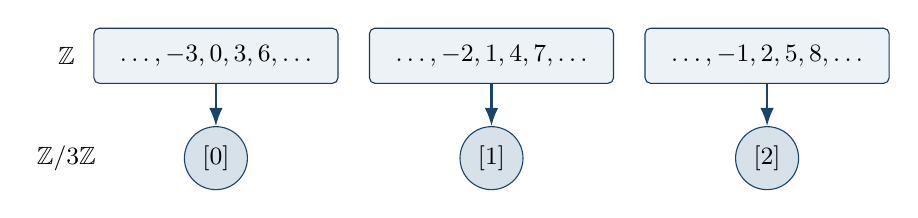
\begin{tikzpicture}[>=Latex,font=\small]
  \node[font=\small] at (-1.9,1.25) {$\Z$};
  \node[font=\small] at (-1.9,-.05) {$\Z/3\Z$};
  \node[draw=manifoldblue!65!black,fill=manifoldblue!8,
        rounded corners=2pt,minimum width=3.1cm,minimum height=.7cm]
        (c0) at (0,1.25) {$\ldots,-3,0,3,6,\ldots$};
  \node[draw=manifoldblue!65!black,fill=manifoldblue!8,
        rounded corners=2pt,minimum width=3.1cm,minimum height=.7cm]
        (c1) at (3.5,1.25) {$\ldots,-2,1,4,7,\ldots$};
  \node[draw=manifoldblue!65!black,fill=manifoldblue!8,
        rounded corners=2pt,minimum width=3.1cm,minimum height=.7cm]
        (c2) at (7,1.25) {$\ldots,-1,2,5,8,\ldots$};
  \node[draw=manifoldblue!75!black,fill=manifoldblue!18,
        circle,minimum size=.8cm] (r0) at (0,-.05) {$[0]$};
  \node[draw=manifoldblue!75!black,fill=manifoldblue!18,
        circle,minimum size=.8cm] (r1) at (3.5,-.05) {$[1]$};
  \node[draw=manifoldblue!75!black,fill=manifoldblue!18,
        circle,minimum size=.8cm] (r2) at (7,-.05) {$[2]$};
  \draw[->,thick,manifoldblue!75!black] (c0)--(r0);
  \draw[->,thick,manifoldblue!75!black] (c1)--(r1);
  \draw[->,thick,manifoldblue!75!black] (c2)--(r2);
\end{tikzpicture}
\caption{Iloraz $\Z/3\Z$: wszystkie liczby w danym
górnym polu mają tę samą resztę, więc odwzorowanie ilorazowe
utożsamia je z jedną klasą.}
\label{fig:reszty-modulo-3-5}
\end{figure}

\section{Moduły, homomorfizmy i ilorazy}
\label{sec:moduly}

Przez $R$ oznaczamy pierścień przemienny z jedynką
$1\ne0$ w sensie Definicji~\ref{def:pierscien-przemienny}.
Pozwala to traktować wszystkie moduły
jednakowo, bez rozróżniania strony działania.
Wiele definicji działa również dla pierścieni
nieprzemiennych i modułów lewych; zaznaczymy,
gdzie przemienność upraszcza zapis.
Moduł można traktować jak przestrzeń liniową, w której
skalary nie muszą mieć odwrotności. W szczególności
wektory kratowe $\Z^2$ można dodawać i mnożyć przez
liczby całkowite, lecz połowa wektora $(1,0)$
nie należy do tej kraty.

\begin{definicja}[Moduł nad pierścieniem]
\index{modul nad pierscieniem@Moduł nad pierścieniem}
\label{def:modul}
\emph{Moduł $M$ nad $R$} to grupa abelowa
$(M,+,0)$ z mnożeniem przez skalary
$R\times M\to M$, $(r,m)\mapsto rm$, takim że
dla $r,s\in R$ i $m,n\in M$ mamy
\[
 (r+s)m=rm+sm,\qquad r(m+n)=rm+rn,\qquad
 (rs)m=r(sm),\qquad 1m=m.
\]
Grupa abelowa oznacza tutaj, że dodawanie w $M$
jest łączne, przemienne, ma element $0$ i każdy
element $m$ ma element przeciwny $-m$.
\end{definicja}

Aksjomaty wymuszają $0_Rm=0_M$ i $r0_M=0_M$:
na przykład $0_Rm=(0_R+0_R)m=0_Rm+0_Rm$,
więc skracamy w grupie addytywnej $M$; dla drugiej
równości stosujemy $r(0_M+0_M)=r0_M+r0_M$.
Ponadto $m+(-1_R)m=(1_R-1_R)m=0_M$,
czyli $(-1_R)m=-m$.

Definicja różni się od definicji przestrzeni liniowej
jedynie tym, że nie wymagamy dzielenia przez
niezerowy skalar. Ta różnica ma poważne skutki:
moduł może nie mieć bazy, a równanie $rm=0$ może
zachodzić dla $r\ne0$ i $m\ne0$.
W przypadku grup abelowych, czyli $\Z$-modułów,
opisujemy to precyzyjnie następująco.

\begin{definicja}[Element torsyjny i $m$-torsja]
\label{def:torsja}
Element $x$ grupy abelowej $M$ jest
\emph{torsyjny}, jeśli istnieje liczba całkowita
$k\ne0$ taka, że $kx=0$. Zbiór takich elementów
oznaczamy $\operatorname{Tors}(M)$ i nazywamy
\emph{podgrupą torsyjną}. Dla ustalonego $m\geq2$
definiujemy \emph{$m$-torsję}
$M[m]:=\{x\in M:mx=0\}=\ker(\times m:M\to M)$.
Podgrupa $M[m]$ składa się z elementów zabijanych
przez tę jedną liczbę $m$; cały
$\operatorname{Tors}(M)$ dopuszcza różne niezerowe
liczby dla różnych elementów.
\end{definicja}

Oba zbiory są rzeczywiście podgrupami: jeśli
$kx=0$ i $\ell y=0$, to $k\ell(x-y)=0$;
dla ustalonego $m$ mamy od razu
$m(x-y)=mx-my=0$. Na przykład
$\operatorname{Tors}(\Z\oplus\Z/2)
=0\oplus\Z/2$, podczas gdy $\Z$
nie ma niezerowej torsji.
W $M=\Z/6\Z$ wszystkie elementy są torsyjne,
ale $M[2]=\{[0],[3]\}$ i
$M[3]=\{[0],[2],[4]\}$. Na przykład
$2[k]=[0]$ dokładnie wtedy, gdy $6$ dzieli $2k$,
czyli $3$ dzieli $k$. Pokazuje to różnicę między
torsją o ustalonym wykładniku a całą podgrupą torsyjną.

\begin{przyklad}[Od grup abelowych do spinorów]
\label{prz:moduly-podstawowe}
\begin{enumerate}[leftmargin=*]
\item Każda przestrzeń liniowa nad ciałem
      $\mathbb K$ jest $\mathbb K$-modułem.
\item $R^n$ z dodawaniem i mnożeniem współrzędnych
      przez skalary jest wolnym $R$-modułem o bazie
      $e_1,\ldots,e_n$. W szczególności $\Z^2$
      jest modułem wolnym, choć nie jest przestrzenią
      liniową nad $\Z$, bo $\Z$ nie jest ciałem.
\item Każda grupa abelowa $A$ jest $\Z$-modułem:
      $na$ dla $n>0$ oznacza sumę $n$ kopii $a$,
      $0a=0$, a $(-n)a=-(na)$. Aksjomaty modułu
      wynikają z praw dodawania. Odwrotnie,
      w każdym $\Z$-module aksjomaty wymuszają
      właśnie tę regułę, więc pojęcia są równoważne.
\item Dla $m\geq2$ grupa $\Z/m\Z$ jest $\Z$-modułem;
      niezerowa klasa $[1]$ spełnia $m[1]=0$. Nie ma bazy
      nad $\Z$. Istotnie, gdyby $[1]=\sum_i a_i e_i$ w takiej
      bazie, równość $\sum_i ma_i e_i=0$ i jednoznaczność
      współczynników wymuszałyby $ma_i=0$ w $\Z$ dla każdego $i$.
      Stąd wszystkie $a_i=0$, sprzecznie z $[1]\ne0$.
\item $R/I$ dla ideału $I\subseteq R$ jest
      $R$-modułem: $r[s]=[rs]$. Działanie jest
      dobrze określone, gdyż z $s-s'\in I$
      wynika $r(s-s')\in I$.
      Sam ideał $I$ jest podmodułem modułu $R$.
\item Moduł spinorów z Definicji~\ref{def:spinor}
      jest modułem nad zespoloną algebrą
      Clifforda. Tam algebra może być
      nieprzemienna i działanie jest \emph{lewe};
      jest to przykład szerszego pojęcia modułu lewego.
      W głównej części obecnego rozdziału ograniczamy się
      do pierścieni przemiennych, wystarczających
      w podstawowych przykładach grup homologii.
\end{enumerate}
\end{przyklad}

\begin{definicja}[Podmoduł, homomorfizm i moduł wolny]
\index{podmodul homomorfizm modul wolny@Podmoduł, homomorfizm, moduł wolny}
\label{def:modul-map}
Podzbiór $N\subseteq M$ jest \emph{podmodułem}, jeśli zawiera $0$
i jest zamknięty na dodawanie, branie elementów przeciwnych
oraz mnożenie przez elementy $R$.
\emph{Homomorfizm $R$-modułów} $f:M\to N$ spełnia
$f(m+m')=f(m)+f(m')$ i $f(rm)=rf(m)$.
Zbiór takich homomorfizmów oznaczamy przez $\operatorname{Hom}_R(M,N)$.

Moduł \emph{wolny} z bazą $(e_i)_{i\in I}$ ma tę własność,
że każdy element jest jednoznaczną skończoną sumą
$\sum_{i\in I}r_i e_i$. Modelem jest $R^{(I)}$, czyli rodziny
współczynników o skończonym nośniku. Suma prosta $M\oplus N$
składa się z par $(m,n)$ z działaniami składowymi.
\end{definicja}

Przy dodawaniu punktowym i działaniu $(rf)(m)=r f(m)$
zbiór $\operatorname{Hom}_R(M,N)$ jest $R$-modułem.
Przemienność $R$ zapewnia $R$-liniowość $rf$:
$(rf)(sm)=rsf(m)=s(rf)(m)$.
Na przykład $\operatorname{Hom}_{\Z}(\Z/2,\Z)=0$,
bo obraz klasy $[1]$ musiałby być elementem $\Z$ zabijanym przez $2$.

\begin{stwierdzenie}[Homomorfizmy wyznaczone przez generator]
\label{prop:hom-cyclic-5}
Dla $R$-modułu $M$ odwzorowanie $f\mapsto f(1)$ daje
izomorfizm $\operatorname{Hom}_R(R,M)\cong M$.
Dla grupy abelowej $A$ i $n\geq2$ analogicznie
$\operatorname{Hom}_{\Z}(\Z/n\Z,A)\cong A[n]$,
przy czym izomorfizm wysyła $f$ na $f([1])$.
\end{stwierdzenie}
\begin{proof}
Liniowość daje $f(r)=rf(1)$, więc wartość w $1$
wyznacza $f:R\to M$. Odwrotnie, dla dowolnego $m\in M$
wzór $f_m(r)=rm$ definiuje homomorfizm z $f_m(1)=m$.
Oba przyporządkowania zachowują dodawanie i mnożenie
przez skalary, więc są odwrotnymi izomorfizmami.

Jeśli $f:\Z/n\Z\to A$, to
$nf([1])=f(n[1])=f([0])=0$, zatem $f([1])\in A[n]$.
Dla $x\in A[n]$ wzór $f_x([k])=kx$ jest dobrze określony:
gdy $[k]=[\ell]$, mamy $k-\ell=qn$ i
$kx-\ell x=qn x=0$. Wzór jest addytywny,
a $f_x([1])=x$. Znów dostajemy odwrotne homomorfizmy.
\end{proof}

Na przykład $\operatorname{Hom}_{\Z}(\Z/6\Z,\Z/4\Z)$
ma dwa elementy: obraz $[1]$ może być tylko $[0]$
albo $[2]$, bo tylko te klasy w $\Z/4\Z$ są
zabijane przez $6$. Istotnie, $6[k]_4=[0]_4$ oznacza
$4\mid6k$, równoważnie $2\mid k$; spośród reprezentantów
$0,1,2,3$ warunek spełniają dokładnie $0$ i $2$.

\begin{definicja}[Moduł ilorazowy]
\index{modul ilorazowy@Moduł ilorazowy}
\label{def:modul-ilorazowy}
Niech $M$ będzie $R$-modułem, a $N\subseteq M$ jego podmodułem.
Na $M$ wprowadzamy relację $m\sim m'$ wtedy i tylko wtedy,
gdy $m-m'\in N$. Jest to relacja równoważności:
zwrotność wynika z $0\in N$, symetria z zamknięcia na
elementy przeciwne, a przechodniość z zamknięcia na dodawanie.
Klasę elementu $m\in M$ oznaczamy przez $[m]=m+N$.
Zbiór $M/N:=\{m+N:m\in M\}$ nazywamy
\emph{modułem ilorazowym} $M$ przez $N$.
Klasa $m+N$ jest kopią podmodułu $N$ przesuniętą o $m$.
W ilorazie wszystkie jej punkty stają się jednym elementem.

Działania definiujemy przez $[m]+[m']=[m+m']$ oraz
$r[m]=[rm]$. Są dobrze określone. Istotnie, jeśli
$m-\widetilde m\in N$ i $m'-\widetilde m'\in N$, to
\[
(m+m')-(\widetilde m+\widetilde m')
=
(m-\widetilde m)+(m'-\widetilde m')
\in N,
\]
a dla $r\in R$ mamy $rm-r\widetilde m=r(m-\widetilde m)\in N$.
\end{definicja}

Naturalne odwzorowanie $\pi\colon M\to M/N$, $\pi(m)=[m]$,
jest surjektywnym homomorfizmem $R$-modułów o jądrze
$\ker\pi=N$.
Otrzymujemy więc krótki ciąg dokładny
\[
0\longrightarrow N
\overset{\iota}{\longrightarrow} M
\overset{\pi}{\longrightarrow}M/N
\longrightarrow0.
\]
Tutaj $\iota$ jest inkluzją. Słowo \emph{dokładny} oznacza,
że w każdym środkowym miejscu obraz poprzedniej strzałki
jest jądrem następnej: $\ker\iota=0$,
$\operatorname{im}\iota=N=\ker\pi$ oraz
$\operatorname{im}\pi=M/N$.

\begin{stwierdzenie}[Własność modułu ilorazowego]
\label{prop:module-quotient-universal-5}
Dla homomorfizmu $R$-modułów $f:M\to P$ istnieje
homomorfizm $\bar f:M/N\to P$ spełniający
$f=\bar f\circ\pi$ dokładnie wtedy, gdy
$N\subseteq\ker f$. Wtedy $\bar f$ jest jedyny
i $\bar f([m])=f(m)$.
\end{stwierdzenie}
\begin{proof}
Jeśli $f=\bar f\circ\pi$ i $n\in N$, to
$f(n)=\bar f([n])=\bar f([0])=0$.
Odwrotnie, jeśli $N\subseteq\ker f$, to z
$[m]=[m']$ wynika $m-m'\in N$ i
$f(m)-f(m')=f(m-m')=0$. Wzór na $\bar f$
jest więc dobrze określony. Zachowuje dodawanie
i mnożenie przez skalary, ponieważ robi to $f$.
Równość $f=\bar f\circ\pi$ zachodzi na każdym $m$,
a surjektywność $\pi$ zapewnia jednoznaczność $\bar f$.
\end{proof}

\noindent\emph{Porównanie w Bibliotece matematycznej:} \atlasref{AA-16::aa:tw:modules-first-isomorphism}{AA-16: pierwsze twierdzenie o izomorfizmie modułów}.

\begin{twierdzenie}[Pierwsze twierdzenie o izomorfizmie]
\label{thm:modul-izomorfizm}
Dla homomorfizmu $f:M\to P$ jądro i obraz są podmodułami,
a odwzorowanie
\[
\overline f:M/\ker f\longrightarrow\operatorname{im}f,
\qquad [m]\longmapsto f(m)
\]
jest izomorfizmem $R$-modułów.
\end{twierdzenie}
\begin{proof}
Jeśli $f(m)=f(m')=0$, to $f(m-m')=0$ i $f(rm)=0$;
zatem jądro jest podmodułem. Obraz jest nim, ponieważ
$f(m)+f(m')=f(m+m')$ oraz $rf(m)=f(rm)$.
Jeśli $[m]=[m']$ modulo $\ker f$, to $f(m-m')=0$,
więc $f(m)=f(m')$: wzór jest dobrze określony.
Jest liniowy i surjektywny na obraz. Równość
$\overline f([m])=0$ oznacza $m\in\ker f$, czyli $[m]=[0]$;
stąd jest również injektywny.
\end{proof}

\begin{przyklad}
Dla $M=\Z$ i $N=m\Z$ otrzymujemy $M/N=\Z/m\Z$.
Jest to moduł nad $\Z$, lecz dla $m>1$ nie jest modułem wolnym.
Przykład ten pokazuje, że iloraz modułu wolnego przez podmoduł
nie musi być modułem wolnym.

Dla $M=\R^2$ i $N=\R(1,0)$ odwzorowanie
$f(x,y)=y$ ma jądro $N$. Pierwsze twierdzenie
o izomorfizmie daje $\R^2/\R(1,0)\cong\R$;
izomorfizm wysyła $[(x,y)]$ na $y$.
Klasa punktu $(x,y)$ jest całą poziomą prostą
$\{(x+t,y):t\in\R\}$: w ilorazie zapamiętujemy tylko
wysokość $y$, jak na Rysunku~\ref{fig:modul-iloraz-poziome-5}.

Z kolei homomorfizm
$\Z^2\to\Z/2\Z\oplus\Z/3\Z$ dany przez
$(a,b)\mapsto([a]_2,[b]_3)$ jest surjektywny,
a jego jądrem jest $2\Z\oplus3\Z$. Stąd
$\Z^2/(2\Z\oplus3\Z)\cong\Z/2\Z\oplus\Z/3\Z$.
Ten iloraz jest skończony i torsyjny, mimo że
$\Z^2$ i jego podmoduł są wolne.
\end{przyklad}

\begin{figure}[htbp]
\centering
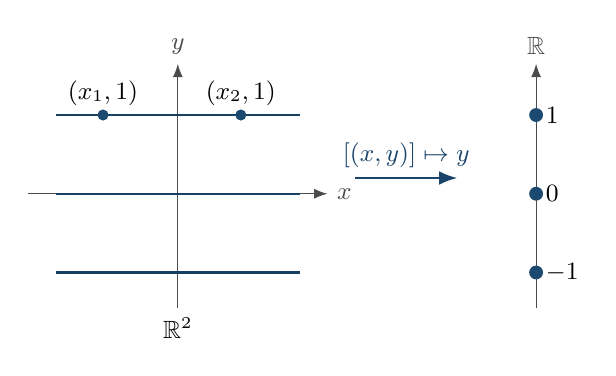
\begin{tikzpicture}[>=Latex,font=\small]
  \draw[->,black!70] (-1.9,0)--(1.9,0) node[right] {$x$};
  \draw[->,black!70] (0,-1.45)--(0,1.65) node[above] {$y$};
  \draw[manifoldblue!70!black,thick] (-1.55,-1)--(1.55,-1);
  \draw[manifoldblue!70!black,thick] (-1.55,0)--(1.55,0);
  \draw[manifoldblue!70!black,thick] (-1.55,1)--(1.55,1);
  \fill[manifoldblue!80!black] (-.95,1) circle (2pt);
  \fill[manifoldblue!80!black] (.8,1) circle (2pt);
  \node[above] at (-.95,1) {$(x_1,1)$};
  \node[above] at (.8,1) {$(x_2,1)$};
  \node[below] at (0,-1.45) {$\R^2$};
  \draw[->,thick,manifoldblue!75!black] (2.25,.2)--(3.55,.2)
        node[midway,above] {$[(x,y)]\mapsto y$};
  \draw[->,black!70] (4.55,-1.45)--(4.55,1.65) node[above] {$\R$};
  \foreach \v in {-1,0,1}{
    \fill[manifoldblue!80!black] (4.55,\v) circle (2.5pt);
  }
  \node[right] at (4.55,1) {$1$};
  \node[right] at (4.55,0) {$0$};
  \node[right] at (4.55,-1) {$-1$};
\end{tikzpicture}
\caption{Iloraz $\R^2/\R(1,0)$: każda pozioma prosta
jest jedną klasą. Dwa zaznaczone punkty na wysokości $1$
mają ten sam obraz.}
\label{fig:modul-iloraz-poziome-5}
\end{figure}

\begin{stwierdzenie}[Wymiar przestrzeni ilorazowej]
\index{modul ilorazowy!wymiar}
\label{prop:wymiar-ilorazu}
Niech $\mathbb K$ będzie ciałem, $M$ skończenie wymiarową
$\mathbb K$-przestrzenią wektorową, a $N\subseteq M$ podprzestrzenią.
Wówczas
\[
\dim_{\mathbb K}(M/N)
=
\dim_{\mathbb K}M-\dim_{\mathbb K}N.
\]
\end{stwierdzenie}

\begin{proof}
Niech $e_1,\ldots,e_k$ będzie bazą $N$.
Uzupełnijmy ją do bazy $e_1,\ldots,e_k,e_{k+1},\ldots,e_n$
przestrzeni $M$. Pokażemy, że klasy
$[e_{k+1}],\ldots,[e_n]$ tworzą bazę $M/N$.

Każdy $m\in M$ ma jednoznaczne współrzędne w tej bazie.
Pierwsza część jego rozkładu leży w $N$, więc
\[
\begin{aligned}
m&=\underbrace{\sum_{i=1}^k a_i e_i}_{\in N}
   +\sum_{i=k+1}^n a_i e_i,\\
[m]&=\sum_{i=k+1}^n a_i[e_i].
\end{aligned}
\]
Wskazane klasy generują zatem $M/N$.

Jeśli $\sum_{i=k+1}^n a_i[e_i]=[0]$, to
$v:=\sum_{i=k+1}^n a_i e_i\in N$.
Możemy więc zapisać $v=\sum_{i=1}^k b_i e_i$.
Jednoznaczność rozwinięcia względem pełnej bazy
wymusza $a_{k+1}=\cdots=a_n=0$.
Klasy są liniowo niezależne, więc tworzą bazę
$M/N$ o $n-k$ elementach. To daje żądany wzór.
\end{proof}

Dla modułów nad dziedziną całkowitości analogiczny wzór
sformułujemy po zdefiniowaniu iloczynu tensorowego modułów.

\section{Iloczyn tensorowy modułów}
\label{sec:tensor-modulow-algebra}
\index{iloczyn tensorowy modulow@Iloczyn tensorowy modułów}

W Rozdziale~\ref{ch:algebra-tensorowa} konstruowaliśmy iloczyny tensorowe
przestrzeni liniowych nad ciałem. Nad pierścieniem
budujemy podobny obiekt, lecz nie wolno już korzystać
z bazy dowolnego modułu. Intuicja pozostaje ta sama:
symbol $m\otimes n$ ma być liniowy w obu argumentach,
a każda dwuliniowa reguła na parach powinna przechodzić
przez jedno odwzorowanie liniowe.
Różnica względem przestrzeni liniowych ujawni się już w przykładzie:
utworzenie iloczynu tensorowego z $R/I$ narzuca w drugim czynniku relacje $im=0$
dla wszystkich $i\in I$, nawet jeśli wcześniej $im\ne0$.

\begin{definicja}[Iloczyn tensorowy modułów]
\label{def:tensor-modulow}
Niech $M,N$ będą $R$-modułami. Weźmy wolny
$R$-moduł $F=R^{(M\times N)}$ na formalnych
symbolach $[(m,n)]$, po jednym dla każdej pary $(m,n)$.
Nawias kwadratowy oznacza tu generator wolnego modułu;
dopiero $[(m,n)]+K$ będzie jego klasą w ilorazie.
Niech $K\subseteq F$ będzie
podmodułem generowanym przez wszystkie elementy
\[
\begin{aligned}
 &[(m+m',n)]-[(m,n)]-[(m',n)],\\
 &[(m,n+n')]-[(m,n)]-[(m,n')],\\
 &[(rm,n)]-r[(m,n)],\qquad [(m,rn)]-r[(m,n)],
\end{aligned}
\]
gdzie $m,m'\in M$, $n,n'\in N$ i $r\in R$.
\emph{Iloczyn tensorowy} to $M\otimes_R N=F/K$,
a $m\otimes n$ oznacza klasę $[(m,n)]+K$.
\end{definicja}

Podmoduł generowany przez relacje składa się
z ich \emph{skończonych} kombinacji $R$-liniowych.
To jest algebraiczny sens narzucenia relacji.
Ukończony iloczyn tensorowy jest innym pojęciem:
wymaga dodatkowej topologii lub normy na modułach
i nie występuje w tej konstrukcji.
Z definicji
$rm\otimes n=m\otimes rn=r(m\otimes n)$.
Ponadto $(0+0)\otimes n=0\otimes n+0\otimes n$,
więc $0\otimes n=0$; analogicznie $m\otimes0=0$.
Każdy element jest skończoną sumą tensorów
prostych, lecz nie musi być jednym tensorem prostym.
Przykład sumy niebędącej tensorem prostym pojawił się już
w Rozdziale~\ref{ch:algebra-tensorowa}; nad pierścieniem
nie możemy go na ogół rozpoznać za pomocą macierzy
współczynników, bo moduły nie muszą mieć baz.

\begin{twierdzenie}[Własność uniwersalna iloczynu tensorowego]
\label{thm:tensor-modulow-uniwersalnosc}
Dla każdego $R$-modułu $P$ i każdego
odwzorowania $R$-dwuliniowego
$b:M\times N\to P$ istnieje dokładnie
jeden homomorfizm $\widetilde b:M\otimes_R N\to P$
spełniający $\widetilde b(m\otimes n)=b(m,n)$.
\end{twierdzenie}
\begin{proof}
Na wolnym module $F$ istnieje dokładnie
jeden homomorfizm $L:F\to P$ z
$L([(m,n)])=b(m,n)$: określamy go na bazie
i przedłużamy liniowo. Addytywność i
$R$-liniowość $b$ w każdej zmiennej oznaczają,
że $L$ zeruje cztery rodzaje generatorów $K$.
Stąd $K\subseteq\ker L$, więc wzór
$\widetilde b(x+K)=L(x)$ jest dobrze określony.
Tensory proste rozpinają iloraz $F/K$;
wartości na nich wymuszają jednoznaczność.
Jeśli para $(T,\tau)$ również spełnia podaną własność,
stosujemy ją do odwzorowania $(m,n)\mapsto m\otimes n$
i otrzymujemy $\alpha:T\to M\otimes_R N$. Własność właśnie
skonstruowanego iloczynu daje w drugą stronę
$\beta:M\otimes_R N\to T$, wysyłające $m\otimes n$ na
$\tau(m,n)$. Złożenie $\beta\circ\alpha$ spełnia
$(\beta\circ\alpha)(\tau(m,n))=\tau(m,n)$, zatem
jest $\id_T$ przez jednoznaczność we własności $(T,\tau)$.
Analogicznie $\alpha\circ\beta$ jest $\id_{M\otimes_R N}$
przez właśnie dowiedzioną jednoznaczność.
To uzasadnia kanoniczność konstrukcji.
\end{proof}

\begin{przyklad}[Jednostka i iloraz przez ideał]
\label{prz:tensor-jednostka-ideal}
Odwzorowanie $R\otimes_R M\to M$,
$r\otimes m\mapsto rm$, jest izomorfizmem;
jego odwrotność wysyła $m$ na $1\otimes m$.
Oba złożenia sprawdzamy na generatorach:
$m\mapsto1\otimes m\mapsto m$ oraz
$r\otimes m\mapsto rm\mapsto1\otimes rm=r\otimes m$.
Ostatnia równość jest relacją przenoszącą skalar między czynnikami.
Jeśli $I\subseteq R$ jest ideałem, połóżmy
$IM=\{\sum_{j=1}^q i_jm_j:
i_j\in I,\ m_j\in M\}$.
Wówczas
\begin{equation}\label{eq:tensor-ideal-iloraz}
 (R/I)\otimes_R M\cong M/IM,
 \qquad (r+I)\otimes m\longmapsto rm+IM.
\end{equation}
Istotnie, wzór jest dwuliniowy i nie zależy
od wyboru $r$, bo $i m\in IM$ dla $i\in I$.
Odwrotność wysyła $m+IM$ na
$(1+I)\otimes m$. Jeśli $i\in I$, to
$(1+I)\otimes im=(i+I)\otimes m=0$;
znika więc na całym $IM$. Oba złożenia
są identycznościami na generatorach.
Dla $R=\Z$ i $I=m\Z$ otrzymujemy
$(\Z/m)\otimes_{\Z}A\cong A/mA$.
\end{przyklad}

\begin{przyklad}[Iloczyn tensorowy modułów cyklicznych]
Dla dodatnich liczb całkowitych $m,n$ wzór
\eqref{eq:tensor-ideal-iloraz} daje
\[
 (\Z/m)\otimes_{\Z}(\Z/n)
 \cong (\Z/n)/m(\Z/n)
 \cong \Z/(m\Z+n\Z)
 \cong \Z/\gcd(m,n).
\]
Środkowy izomorfizm pochodzi z surjekcji
$\Z/n\to\Z/(m\Z+n\Z)$, $[a]_n\mapsto a+(m\Z+n\Z)$.
Jest ona dobrze określona, bo $n\Z\subseteq m\Z+n\Z$.
Jej jądro to $m(\Z/n)$: warunek $a=mk+n\ell$
jest równoważny $[a]_n=m[k]_n$.
Stosujemy Twierdzenie~\ref{thm:modul-izomorfizm}.

Wyjaśnijmy też ostatnią równość ideałów. Na mocy
Stwierdzenia~\ref{prop:idealy-Z-5} niezerowy ideał
$m\Z+n\Z$ ma postać $d\Z$, gdzie $d>0$.
Ponieważ $m,n\in d\Z$, liczba $d$ dzieli oba.
Z kolei $d\in m\Z+n\Z$ daje $d=um+vn$
dla pewnych $u,v\in\Z$; każdy wspólny dzielnik $m,n$
dzieli więc $d$. Stąd $d=\gcd(m,n)$.
Jest to zarazem tożsamość Bézouta użyta w tym rachunku.
Na przykład $6(\Z/4)=\{[0]_4,[2]_4\}=2(\Z/4)$,
więc $(\Z/6)\otimes_{\Z}(\Z/4)\cong\Z/2$.
Natomiast $(\Z/2)\otimes_{\Z}(\Z/3)=0$:
mnożenie przez $2$ jest surjekcją na $\Z/3$,
gdyż klasy $[0]_3,[1]_3,[2]_3$ przechodzą odpowiednio
na $[0]_3,[2]_3,[1]_3$. Zatem $2(\Z/3)=\Z/3$.
\end{przyklad}

\begin{stwierdzenie}[Iloczyn tensorowy odwzorowań]
\label{prop:tensor-maps-algebra}
Homomorfizm $f:M\to M'$ indukuje
$f\otimes\id_N:M\otimes_R N\to M'\otimes_R N$
przez $(f\otimes\id_N)(m\otimes n)=f(m)\otimes n$.
Jeśli $f$ jest surjekcją, to $f\otimes\id_N$
jest surjekcją. Funktor $-\otimes_R N$ nie musi
zachowywać iniekcji.
\end{stwierdzenie}
\begin{proof}
Dwuliniowość odwzorowania $(m,n)\mapsto f(m)\otimes n$
i Twierdzenie~\ref{thm:tensor-modulow-uniwersalnosc}
dają indukowany homomorfizm.
Gdy $f$ jest surjekcją, każdy tensor prosty
$m'\otimes n$ ma przeciwobraz $m\otimes n$
z $f(m)=m'$. Tensory proste rozpinają cel,
więc indukowany homomorfizm jest surjekcją.
Dla iniekcji $f=\times2:\Z\to\Z$ oraz
$N=\Z/2$ identyfikacja
$\Z\otimes_{\Z}\Z/2\cong\Z/2$ pokazuje,
że $f\otimes\id_N$ jest odwzorowaniem zerowym:
$(2z)\otimes[1]=z\otimes[2]=0$.
Nie jest zatem iniekcją.
\end{proof}

\begin{stwierdzenie}[Dokładność po prawej stronie]
\label{prop:tensor-prawostronnie-dokladny}
\index{iloczyn tensorowy!dokładność po prawej stronie}
Jeśli ciąg $R$-modułów
\[
 M_1\xrightarrow{f}M_2\xrightarrow{q}M_3\longrightarrow0
\]
jest dokładny, to dla każdego $R$-modułu $N$ dokładny jest także
\[
 M_1\otimes_R N\xrightarrow{f\otimes\id_N}
 M_2\otimes_R N\xrightarrow{q\otimes\id_N}
 M_3\otimes_R N\longrightarrow0.
\]
Nie ma analogicznej gwarancji iniektywności na lewym końcu.
\end{stwierdzenie}
\begin{proof}
Ponieważ $q$ jest surjekcją, taka jest również $q\otimes\id_N$.
Równość $q\circ f=0$ daje
$\operatorname{im}(f\otimes\id_N)\subseteq\ker(q\otimes\id_N)$.
Oznaczmy iloraz $(M_2\otimes_R N)/\operatorname{im}(f\otimes\id_N)$
przez $Q$. Dla $x\in M_3$ wybierzmy podniesienie
$\widehat x\in M_2$ i połóżmy
$b(x,n)=[\widehat x\otimes n]\in Q$.
Jeśli $\widehat x'$ jest innym podniesieniem, to
$\widehat x-\widehat x'\in\ker q=\operatorname{im}f$;
stąd obie klasy są równe. Podniesienia sumy oraz
sumy podniesień różnią się elementem $\ker q$,
podobnie jak podniesienia $rx$ oraz $r\widehat x$.
Dlatego $b$ jest $R$-dwuliniowe. Własność uniwersalna
daje homomorfizm $V:M_3\otimes_R N\to Q$.
W drugą stronę $q\otimes\id_N$ zeruje
$\operatorname{im}(f\otimes\id_N)$ i schodzi do
$U:Q\to M_3\otimes_R N$.
Dla $x\otimes n$ złożenie daje
$(U\circ V)(x\otimes n)=q(\widehat x)\otimes n=x\otimes n$.
Z kolei $(V\circ U)([m\otimes n])=[m\otimes n]$,
bo jako podniesienie $q(m)$ możemy wybrać samo $m$.
Takie elementy rozpinają odpowiednie moduły,
więc $U,V$ są wzajemnie odwrotne.
W szczególności $q\otimes\id_N$ jest złożeniem projekcji
na $Q$ z izomorfizmem $U$, a jego jądro jest jądrem tej projekcji.
To dokładnie równość
$\ker(q\otimes\id_N)=\operatorname{im}(f\otimes\id_N)$.
\end{proof}

\begin{definicja}[Rozszerzenie skalarów]
\label{def:rozszerzenie-skalarow}
\index{rozszerzenie skalarów}
Jeśli $\varphi:R\to S$ jest homomorfizmem
pierścieni przemiennych z jedynką, to $S$
staje się $R$-modułem przez $r\cdot s=\varphi(r)s$.
Na $M\otimes_R S$ działa $S$ przez
$s\cdot(m\otimes a)=m\otimes sa$.
Ten $S$-moduł nazywamy \emph{rozszerzeniem
skalarów} modułu $M$ wzdłuż $\varphi$.
\end{definicja}

Sprawdźmy relację zbalansowania dla działania
$S$: dla $r\in R$ oraz $s,a\in S$ mamy
\[
 s\cdot((rm)\otimes a)
 =m\otimes\varphi(r)sa
 =m\otimes s\varphi(r)a
 =s\cdot(m\otimes\varphi(r)a).
\]
Przemienność $S$ uzasadnia środkową równość;
relacje addytywności sprawdza się składnikowo.
Dlatego działanie nie zależy od zapisu elementu
jako sumy tensorów prostych. Dla wolnego
$M=\bigoplus_{i\in J}Re_i$ mamy
\[
 M\otimes_R S\cong\bigoplus_{i\in J}Se_i,
 \quad
 (\textstyle\sum_i r_i e_i)\otimes s
 \longmapsto\textstyle\sum_i\varphi(r_i)s e_i.
\]
Odwrotność wysyła $\sum_i s_i e_i$ na
$\sum_i e_i\otimes s_i$; wszystkie sumy są
skończone. Ogólniej, dla rodziny $R$-modułów $(M_i)_{i\in J}$
otrzymujemy izomorfizm
\[
 \left(\bigoplus_{i\in J}M_i\right)\otimes_R N
 \longrightarrow \bigoplus_{i\in J}(M_i\otimes_R N),
 \qquad (m_i)_i\otimes n\longmapsto(m_i\otimes n)_i.
\]
Wzór jest dwuliniowy i ma skończony nośnik, więc określa
homomorfizm przez własność uniwersalną. Odwrotność na
$i$-tym składniku wysyła $m\otimes n$ na $\iota_i(m)\otimes n$,
gdzie $\iota_i$ jest inkluzją do sumy prostej. Oba złożenia są
identycznościami na tensorach prostych, które rozpinają moduły.
Funktor $-\otimes_R N$ zachowuje też izomorfizmy: dla izomorfizmu $f$
odwrotnością $f\otimes\id$ jest $f^{-1}\otimes\id$.
Przykład z $\times2$ ostrzega natomiast przed
wnioskowaniem o dowolnych iniekcjach.
Na przykład po rozszerzeniu skalarów przez
$\R\hookrightarrow\C$ moduł $\R^2$ staje się
$\C^2$: nowe współczynniki są zespolone,
a dwa wektory bazowe pozostają niezależne.

\begin{uwaga}[Moduły rzutowe]
\label{uwaga:moduly-projektywne}
\index{moduł rzutowy}
Moduł $P$ jest \emph{rzutowy}, gdy dla każdej
surjekcji $q:E\twoheadrightarrow B$ i każdego
homomorfizmu $g:P\to B$ istnieje podniesienie
$\widetilde g:P\to E$ z $q\circ\widetilde g=g$.
Równoważnie, $P$ jest składnikiem prostym
pewnego modułu wolnego. Jeśli $P$ jest rzutowy,
wybieramy wolny moduł $F$ na symbolach elementów
$P$ i jego naturalną surjekcję $q:F\twoheadrightarrow P$.
Podnosimy $\id_P$ przez $q$, otrzymując $j:P\to F$
z $q\circ j=\id_P$. Izomorfizm i jego odwrotność to
\[
 P\oplus\ker q\longrightarrow F,\quad (p,k)\longmapsto j(p)+k,
 \qquad
 f\longmapsto\bigl(q(f),f-j(q(f))\bigr).
\]
Drugi składnik ostatniej pary należy do $\ker q$, bo
$q(f-j(q(f)))=q(f)-q(f)=0$.
Złożenie w kierunku $F\to F$ daje $j(q(f))+f-j(q(f))=f$,
a w kierunku $P\oplus\ker q$ daje $(p,k)$, bo $q(k)=0$.
To wyprowadza rozkład $F\cong P\oplus\ker q$. Odwrotnie,
odwzorowanie z wolnego modułu można podnieść,
wybierając przeciwobrazy wartości na bazie.
Jeśli $F=P\oplus Q$, to dla $g:P\to B$
podnosimy $g\circ\operatorname{pr}_P:F\to B$
i ograniczamy otrzymane odwzorowanie do $P$.
Moduł rzutowy nie musi być wolny: dla
$R=\Z/6$ ideał $3R=\{0,3\}$ jest składnikiem
prostym w $R=3R\oplus4R$, lecz jego dwa
elementy wykluczają izomorfizm z $R^{(J)}$.
Rzeczywiście, $3R\cap4R=\{0\}$, a $1=3+4$ w $R$ daje
$r=3r+4r$ dla każdego $r\in R$. Niezerowy moduł wolny
nad $R$ zawiera co najmniej sześć elementów, bo zawiera kopię $R$.
\end{uwaga}

W zastosowaniach do nieprzemiennego pierścienia
grupowego $\Z[\pi]$ rozróżnia się moduł prawy
i lewy. Dla dowolnego pierścienia z jedynką $\Lambda$
oraz prawego modułu $M$ i lewego $N$ zaczynamy od
\emph{wolnej grupy abelowej} na parach $(m,n)$.
Dzielimy ją przez podgrupę generowaną przez relacje
addytywności w obu argumentach oraz
$[(m\lambda,n)]-[(m,\lambda n)]$, $\lambda\in\Lambda$.
Otrzymana grupa abelowa $M\otimes_\Lambda N$ spełnia
$(m\lambda)\otimes n=m\otimes(\lambda n)$.
Każde odwzorowanie do grupy abelowej, addytywne w obu
argumentach i spełniające tę relację, przechodzi przez
dokładnie jeden homomorfizm z iloczynu tensorowego: przedłużamy je
na wolną grupę i dzielimy przez relacje, jak wyżej.
Bez dodatkowych danych wynik nie ma naturalnej struktury
$\Lambda$-modułu. Dla przemiennego $R$ utożsamiamy działanie
prawe z lewym przez $mr=rm$ i odzyskujemy wcześniejszy
$R$-moduł z działaniem $r(m\otimes n)=(rm)\otimes n$.
Na przykład dla prawego modułu regularnego $\Lambda$ zachodzi
$\Lambda\otimes_\Lambda N\cong N$:
$\lambda\otimes n\mapsto\lambda n$, a odwrotność
wysyła $n$ na $1\otimes n$. Relacja zbalansowania daje
$\lambda\otimes n=1\otimes\lambda n$, więc obydwa
złożenia są identycznościami.
Charakteryzacja rzutowości przez podnoszenie i
składniki proste wolnych działa również tam.

\section{Ranga modułu i ciało ułamków}
\label{sec:ranga-modulu}

Po rozszerzeniu skalarów z dziedziny całkowitości $R$ do jej
ciała ułamków moduł staje się przestrzenią wektorową. Jej wymiar
mierzy liczbę niezależnych kierunków, które pozostają po usunięciu
torsji. Pojęcie torsji z Definicji~\ref{def:torsja} dotyczyło
grup abelowych, czyli modułów nad $\Z$. Nad inną dziedziną
musimy wskazać, które skalary mogą zabijać elementy.

\begin{definicja}[Torsja modułu nad dziedziną całkowitości]
\label{def:torsja-r-modulu-5}
Niech $R$ będzie dziedziną całkowitości i $M$ będzie
$R$-modułem. Element $m\in M$ nazywamy
\emph{torsyjnym nad $R$}, jeśli istnieje $r\in R\setminus\{0\}$
takie, że $rm=0$. Przez
\[
 \operatorname{Tors}_R(M)
 :=\{m\in M:\exists r\in R\setminus\{0\},\ rm=0\}
\]
oznaczamy \emph{podmoduł torsyjny}. Moduł jest
\emph{bez torsji}, gdy $\operatorname{Tors}_R(M)=\{0\}$.
Dla $R=\Z$ jest to dokładnie torsja grupy abelowej
z Definicji~\ref{def:torsja}.
\end{definicja}

Uzasadnijmy nazwę \emph{podmoduł}. Jeśli $rm=0$ i $sn=0$,
gdzie $r,s\ne0$, to $rs\ne0$, ponieważ $R$ nie ma
dzielników zera, oraz
\[
 rs(m-n)=s(rm)-r(sn)=0.
\]
Zatem $m-n$ jest torsyjny. Ponadto dla $a\in R$
mamy $r(am)=a(rm)=0$, więc $am$ jest torsyjny.
Element zerowy również należy do tej rodziny.
Wynika stąd zamknięcie na dodawanie, elementy przeciwne
i mnożenie przez skalary.

\begin{przyklad}[Dlaczego potrzebna jest dziedzina całkowitości?]
\label{prz:torsja-z-dzielnikami-zera-5}
W pierścieniu $R=\Z/6\Z$, traktowanym jako
moduł nad samym sobą, mamy $[3][2]=0$
i $[2][3]=0$. Według analogicznego kryterium
elementy $[2]$ i $[3]$ byłyby torsyjne.
Ich suma to jednak $[5]$, będące elementem
odwracalnym ($[5]^2=[1]$). Jeśli
$r[5]=0$, to po pomnożeniu przez $[5]$
otrzymujemy $r=0$. Zatem zbiór elementów
zabijanych przez pewien niezerowy skalar
\emph{nie} byłby zamknięty na dodawanie.
Założenie o braku dzielników zera
nie jest więc tylko wygodą terminologiczną.
\end{przyklad}

\begin{przyklad}[Torsja zależy od pierścienia skalarów]
\label{prz:torsja-wielomiany-5}
Niech $R=\mathbb K[t]$, gdzie $\mathbb K$ jest ciałem,
a $M=R/(t)$. Klasa $[1]$ jest niezerowa w $M$,
ale $t[1]=[t]=0$ i $t\ne0$ w $R$.
Ponieważ każda klasa $[p(t)]$ jest wielokrotnością
$[1]$, wszystkie elementy $M$ są torsyjne nad $R$.
Jako przestrzeń liniowa nad $\mathbb K$ ten sam $M$
jest jednak jednowymiarowy i nie ma torsji
w znaczeniu $\mathbb K$-modułu: niezerowy skalar
ciała jest odwracalny.
Dlatego pojęcia torsji i rangi zawsze wymagają
podania pierścienia skalarów.
\end{przyklad}

\subsection*{Konstrukcja ciała ułamków}

\begin{definicja}[Ciało ułamków]
\label{def:cialo-ulamkow-5}
\index{ciało ułamków}
Niech $R$ będzie dziedziną całkowitości i $S=R\setminus\{0\}$.
Chcemy umożliwić dzielenie przez każdy element $S$.
Na parach $(a,s)\in R\times S$ określamy relację
$(a,s)\sim(b,t)$ wtedy i tylko wtedy, gdy $ta=sb$.
Klasę oznaczamy $a/s$, a zbiór klas przez $K=\operatorname{Frac}(R)$.
Dodawanie i mnożenie mają znane z liczb wymiernych postacie
\[
 \frac as+\frac bt=\frac{ta+sb}{st},\qquad
 \frac as\frac bt=\frac{ab}{st}.
\]
\end{definicja}

\begin{proof}[Poprawność konstrukcji]
Zbiór $S$ zawiera $1$ i jest zamknięty na mnożenie, ponieważ $R$
nie ma dzielników zera. Mianowniki pozostają więc dozwolone.
Zwrotność i symetria relacji są bezpośrednie. Jeśli $ta=sb$ oraz
$ub=tc$, to $t(ua-sc)=0$; skrócenie $t\ne0$ daje $ua=sc$.
Stąd przechodniość.

Jeśli $a/s=a'/s'$ i $b/t=b'/t'$, mamy $s'a=sa'$ oraz $t'b=tb'$.
Po sprowadzeniu sum do wspólnego mianownika korzystamy
w pierwszym składniku z $s'a=sa'$, a w drugim z $t'b=tb'$:
\[
 \begin{aligned}
 s't'(ta+sb)
 &=tt'(s'a)+ss'(t'b)\\
 &=stt'a'+sts'b'=st(t'a'+s'b'),\\
 s't'ab&=(s'a)(t'b)=(sa')(tb')=sta'b'.
 \end{aligned}
\]
Druga równość sprawdza zarazem niezależność iloczynu od przedstawicieli.
Prawa pierścienia wynikają z praw w $R$ po sprowadzeniu do wspólnego
mianownika. Na przykład suma trzech ułamków ma licznik
$tu\,a+su\,b+st\,c$ i mianownik $stu$ niezależnie od nawiasów.
Rozdzielność wynika z rachunku
\[
 \frac as\left(\frac bt+\frac cu\right)
 =\frac{a(ub+tc)}{stu}
 =\frac{uab+tac}{stu}
 =\frac{ab}{st}+\frac{ac}{su}.
\]
W ostatnim kroku obie sumowane klasy sprowadzono do mianownika $stu$.
Zerem jest $0/1$, jedynką $1/1$, a elementem przeciwnym do $a/s$ jest $(-a)/s$.

Równość $a/s=0/1$ zachodzi dokładnie dla $a=0$.
Dla niezerowej klasy $a/s$ element $s/a$ jest więc dozwolony
i $(a/s)(s/a)=1$. Ponadto $0/1\ne1/1$. Otrzymaliśmy ciało.
Odwzorowanie $R\to K$, $a\mapsto a/1$, zachowuje działania i jest
iniektywne; odtąd utożsamiamy $R$ z jego obrazem.
\end{proof}

\begin{stwierdzenie}[Własność uniwersalna ciała ułamków]
Jeśli $j:R\hookrightarrow L$ jest iniektywnym homomorfizmem
do ciała $L$, to istnieje dokładnie jeden homomorfizm ciał
$\widehat j:K\to L$ przedłużający $j$. Jest on dany wzorem
$\widehat j(a/s)=j(a)j(s)^{-1}$.
Jego obraz jest najmniejszym podciałem $L$ zawierającym $j(R)$.
\end{stwierdzenie}
\begin{proof}
Ponieważ $s\ne0$ i $j$ jest iniektywne, $j(s)$ ma odwrotność.
Jeśli $a/s=b/t$, to $ta=sb$, a więc
$j(t)j(a)=j(s)j(b)$; po podzieleniu przez $j(s)j(t)$
otrzymujemy równość wartości wzoru. Dodawanie i mnożenie
ułamków pokazują, że $\widehat j$ jest homomorfizmem.
Każdy homomorfizm ciał przedłużający $j$ musi wysłać
$a/s=(a/1)(s/1)^{-1}$ na $j(a)j(s)^{-1}$,
więc jest jedyny. Obraz składa się z takich ilorazów;
każde podciało zawierające $j(R)$ musi je zawierać.
\end{proof}

\begin{przyklad}[Liczby i funkcje wymierne]
Dla $R=\Z$ konstrukcja daje $\operatorname{Frac}(\Z)=\Q$.
Dla $R=\mathbb K[t]$ otrzymujemy ciało funkcji wymiernych
$\mathbb K(t)$: elementy to ilorazy wielomianów $p(t)/q(t)$ z
$q\ne0$, przy równości przez mnożenie na krzyż. Nie wymagamy,
by mianownik nie miał zer; chodzi o ułamki formalne, nie o funkcje
określone w każdym punkcie $\mathbb K$.
\end{przyklad}

\subsection*{Lokalizacja modułu i jej związek z iloczynem tensorowym}
\index{lokalizacja modułu}

Niech $S=R\setminus\{0\}$. Aby opisać elementy iloczynu tensorowego przez
ułamki, definiujemy \emph{lokalizację} $S^{-1}M$ jako zbiór klas
par $(m,s)\in M\times S$ przy relacji
\[
(m,s)\sim(m',s')
\quad\Longleftrightarrow\quad
t(s'm-sm')=0\text{ dla pewnego }t\in S.
\]
Klasę pary $(m,s)$ oznaczamy $m/s$. Mianowniki stają się tu
odwracalne: dla $M=R$ otrzymujemy $S^{-1}R=K$.
Relacja jest zwrotna i symetryczna. Jeśli
$u(s'm-sm')=0$ i $v(s''m'-s'm'')=0$, to
$uvs'(s''m-sm'')=0$: po rozwinięciu lewa strona
jest sumą $uvs''(s'm-sm')$ oraz
$uvs(s''m'-s'm'')$. Ponieważ $uvs'\in S$,
otrzymujemy przechodniość.
Dodawanie i działanie $K$ określamy przez
\[
\frac{m}{s}+\frac{m'}{s'}=\frac{s'm+sm'}{ss'},
\qquad
\frac{a}{u}\cdot\frac{m}{s}=\frac{am}{us}.
\]
Wzory nie zależą od przedstawicieli. Dla dodawania wynika to
z tożsamości
\[
tt'(s'm+sm')-ss'(t'n+tn')
=t's'(tm-sn)+ts(t'm'-s'n'),
\]
gdy $m/s=n/t$ oraz $m'/s'=n'/t'$; oba składniki po prawej
stronie zeruje iloczyn odpowiednich elementów $S$.
Dokładniej, jeśli $u(tm-sn)=0$ i $v(t'm'-s'n')=0$,
to $uv$ zeruje całą różnicę. Nie trzeba skracać elementów
$S$ w module $M$.
Jeśli ponadto $a/u=b/v$ w $K$, to $va=ub$ i różnica
krzyżowa dla $am/(us)$ i $bn/(vt)$ wynosi
$v a t m-u b s n=v a(t m-s n)$; zeruje ją ten sam element $S$
co różnicę $t m-s n$. Obejmuje to jednoczesną zmianę
przedstawicieli skalara i wektora, więc działanie $K$
jest dobrze określone.

W tym działaniu $a/u$ jest \emph{skalarem} z $K$, a $m/s$ jest
\emph{wektorem} z $S^{-1}M$; nie mnożymy dwóch elementów modułu.
Na $M\otimes_R K$ ten sam skalar działa wzorem
$(a/u)\cdot(m\otimes b/s)=m\otimes ab/(us)$.
Łączność działania na lokalizacji widać z równości
\[
 (a/u)((b/v)(m/s))=(abm)/(uvs)=((a/u)(b/v))(m/s).
\]
Dodawanie jest łączne: obydwa sposoby dodania trzech klas
$m/s$, $m'/s'$ i $m''/s''$ mają przedstawiciela
$(s's''m+ss''m'+ss'm'')/(ss's'')$.
Zerem jest $0/1$, a przeciwną klasą do $m/s$ jest $(-m)/s$.
Na przykład rozdzielność względem dodawania skalarów ma postać
\[
 \left(\frac au+\frac bv\right)\frac ms
 =\frac{(va+ub)m}{uvs}
 =\frac{am}{us}+\frac{bm}{vs}.
\]
Rozdzielność względem dodawania wektorów sprawdza się tak samo
po sprowadzeniu do wspólnego mianownika; $1/1$ działa
identycznie. Dostajemy więc przestrzeń wektorową nad $K$.
W przypadku $M=R$ relacja lokalizacji redukuje się do mnożenia
na krzyż, bo niezerowy $t$ można skrócić w $R$.
W ogólnym module tego robić nie wolno: w $\Z$-module $\Z/2\Z$
element $[1]$ jest niezerowy, lecz $[1]/1=0$ w lokalizacji,
gdyż $2[1]=0$. Właśnie dlatego relacja zawiera dodatkowy czynnik $t$.

\begin{przyklad}[Dwie lokalizacje nad liczbami całkowitymi]
Dla $M=\Z$ mamy $S^{-1}M=\Q$ i na przykład
$(2/3)\cdot(5/7)=10/21$.
Dla $M=\Z\oplus\Z/2\Z$ torsyjny składnik znika:
odwzorowanie $S^{-1}M\to\Q$ określone przez
$(a,[b])/s\mapsto a/s$
jest izomorfizmem, z odwrotnością $a/s\mapsto(a,[0])/s$.
Istotnie, różnicę $(0,[b])/s$ zeruje $2$, a równość dwóch
pierwszych współrzędnych sprawdza się przez mnożenie na krzyż.
\end{przyklad}

\begin{stwierdzenie}[Iloczyn tensorowy z ciałem ułamków]
\label{prop:tensor-cialo-ulamkow}
Niech $R$ będzie dziedziną całkowitości,
$S=R\setminus\{0\}$ i $K=\operatorname{Frac}(R)$.
Dla każdego $R$-modułu $M$ istnieje naturalny izomorfizm
\[
M\otimes_R K\cong S^{-1}M,
\qquad m\otimes\frac{a}{s}\longmapsto\frac{am}{s}.
\]
W szczególności $m/s=0$ dokładnie wtedy, gdy
$tm=0$ dla pewnego $t\in S$.
\end{stwierdzenie}
\begin{proof}
Z definicji lokalizacji
$m/s=0/1$ dokładnie wtedy, gdy pewien $t\in S$
zeruje $m$. Podany wzór jest $R$-dwuliniowy i nie zależy
od wyboru przedstawiciela $a/s\in K$: z $ta=sb$ wynika
$t(am)=s(bm)$. Dlatego przez
Twierdzenie~\ref{thm:tensor-modulow-uniwersalnosc}
określa homomorfizm $M\otimes_R K\to S^{-1}M$.
W drugą stronę kładziemy $m/s\mapsto m\otimes(1/s)$.
Jeśli $(m,s)\sim(m',s')$, to dla pewnego $t\in S$
zachodzi $t(s'm-sm')=0$, a więc
\[
m\otimes\frac1s-m'\otimes\frac1{s'}
=(s'm-sm')\otimes\frac1{ss'}
=t(s'm-sm')\otimes\frac1{tss'}=0.
\]
Odwzorowanie odwrotne jest więc dobrze określone.
Wzór na dodawanie ułamków pokazuje jego addytywność;
zgodność z działaniem $K$ widać na przykład z rachunku
\[
 \frac{am}{us}\longmapsto (am)\otimes\frac1{us}
 =m\otimes\frac{a}{us}
 =\frac au\cdot\left(m\otimes\frac1s\right).
\]
Oba złożenia sprawdzamy bezpośrednio:
$m/s\mapsto m\otimes(1/s)\mapsto m/s$ oraz
$m\otimes(a/s)\mapsto(am)/s\mapsto(am)\otimes(1/s)=m\otimes(a/s)$.
W drugiej równości użyto relacji przenoszącej skalar $a$.
Tensory proste generują cały iloczyn tensorowy,
więc złożenia są identycznościami.
Ponadto dla homomorfizmu $f:M\to M'$ oba sposoby
przeniesienia klasy $m/s$ dają $f(m)/s$;
izomorfizm jest więc naturalny.
\end{proof}

\subsection*{Ranga i jej addytywność}

\begin{definicja}[Ranga modułu nad dziedziną całkowitości]
\index{ranga modułu}
\label{def:ranga-modulu}
Niech $R$ będzie dziedziną całkowitości, a
$K=\operatorname{Frac}(R)$ jej ciałem ułamków.
Rangą $R$-modułu $M$ nazywamy liczbę
\[
\operatorname{rank}_R M
:=
\dim_K(M\otimes_R K),
\]
o ile wymiar po prawej stronie jest skończony.
\end{definicja}

Jeśli $M$ jest wolnym modułem o $n$ generatorach bazowych, to
$M\cong R^n$ i wzór na rozszerzenie skalarów daje
$M\otimes_R K\cong K^n$. Zatem $\operatorname{rank}_R M=n$.

\begin{przyklad}[Ranga nie widzi torsji]
Dla $M=\Z^2\oplus\Z/6$ lokalizacja daje
\[
 M\otimes_{\Z}\Q\longrightarrow\Q^2,\qquad
 ((a,b),[c])\otimes q\longmapsto(qa,qb).
\]
To izomorfizm: jego odwrotność wysyła $(x,y)$ na
$((1,0),[0])\otimes x+((0,1),[0])\otimes y$,
a dla $w=((0,0),[c])$ mamy
$w\otimes q=(6w)\otimes(q/6)=0$, bo $6[c]=0$.
Stąd $\operatorname{rank}_{\Z}M=2$.
Podobnie moduł $\mathbb K[t]/(t)$ ma rangę $0$
nad $\mathbb K[t]$: jego generator $[1]$ jest niezerowy,
ale $t[1]=0$, a $t$ staje się odwracalny w
$\mathbb K(t)$.
\end{przyklad}

\begin{stwierdzenie}[Addytywność rangi]
\index{ranga modułu!addytywnosc@addytywność}
\label{prop:ranga-ilorazu}
Niech $R$ będzie dziedziną całkowitości oraz
$N\subseteq M$ podmodułem. Jeśli odpowiednie rangi są skończone, to
\[
\operatorname{rank}_R M
=
\operatorname{rank}_R N
+
\operatorname{rank}_R(M/N).
\]
W szczególności $\operatorname{rank}_R(M/N)
=\operatorname{rank}_R M-\operatorname{rank}_R N$.
\end{stwierdzenie}

\begin{proof}
Z krótkiego ciągu dokładnego
\[
0\longrightarrow N
\longrightarrow M
\longrightarrow M/N
\longrightarrow0
\]
po utworzeniu iloczynu tensorowego każdego składnika
z ciałem ułamków $K=\operatorname{Frac}(R)$
otrzymujemy ciąg dokładny przestrzeni wektorowych
\[
0
\longrightarrow
N\otimes_R K
\longrightarrow
M\otimes_R K
\longrightarrow
(M/N)\otimes_R K
\longrightarrow0.
\]
Wyjaśnijmy tu krok o dokładności, korzystając z
izomorfizmu~\ref{prop:tensor-cialo-ulamkow}. Jeśli $n/s$
dla $n\in N$ znika w $M\otimes_R K$, to $tn=0$
dla pewnego $t\in S$ już w $N$, więc $n/s=0$ także
w $N\otimes_R K$. Jeśli obraz $m/s$ znika w
$(M/N)\otimes_R K$, to dla pewnego $t\in S$ mamy
$tm\in N$, a więc $m/s=(tm)/(ts)$ należy do obrazu
$N\otimes_R K$. Surjektywność na końcu wynika z
podnoszenia licznika klasy $[m]/s$.
Z Twierdzenia~\ref{thm:modul-izomorfizm} ostatnia przestrzeń
jest izomorficzna z ilorazem $M\otimes_R K$
przez obraz $N\otimes_R K$. Iniektywność pierwszej strzałki
utożsamia ten obraz z $N\otimes_R K$.
Stosując wzór na wymiar ilorazu ze
Stwierdzenia~\ref{prop:wymiar-ilorazu} i przenosząc składnik, dostajemy
\[
\dim_K(M\otimes_R K)
=
\dim_K(N\otimes_R K)
+
\dim_K((M/N)\otimes_R K),
\]
co jest dokładnie żądanym wzorem.
\end{proof}

\begin{przyklad}[Torsja powstała w ilorazie]
Weźmy $M=\Z^2$ oraz podmoduł
$N=2\Z\oplus\{0\}$, którego ranga wynosi $1$.
Odwzorowanie
\[
 M/N\longrightarrow\Z/2\oplus\Z,\qquad
 (a,b)+N\longmapsto([a]_2,b)
\]
jest izomorfizmem: dwie pary mają ten sam obraz
dokładnie wtedy, gdy ich różnica należy do $N$.
Iloraz ma więc niezerowy składnik torsyjny, ale jego
ranga wynosi $1$, zgodnie z równością $2=1+1$.
\end{przyklad}

\begin{uwaga}
Dla ogólnego pierścienia $R$ nie należy bez dodatkowych założeń
pisać wzoru $\dim(M/N)=\dim M-\dim N$.
Pojęcie wymiaru jest naturalne dla przestrzeni wektorowych, natomiast
dla modułów stosuje się między innymi rangę, liczbę generatorów
oraz -- w przypadku skończenie generowanych modułów nad
pierścieniami głównymi -- rozkład
na część wolną i torsyjną.

Na przykład $\Z/2\Z$ ma rangę zerową jako $\Z$-moduł,
mimo że jest modułem niezerowym. Ranga nie wykrywa więc torsji.
\end{uwaga}

\par\smallskip
{\footnotesize\noindent\emph{Dalsza lektura:}
Konstrukcję iloczynu wolnego i jego związek z topologią opisuje
Allen Hatcher, \emph{Algebraic Topology}, sekcja~1.2,
\emph{Free Products of Groups}, s.~41--42,
\url{https://pi.math.cornell.edu/~hatcher/AT/AT.pdf}.
Iloczyn tensorowy nad pierścieniem przemiennym rozwija
\emph{The Stacks Project}, sekcja~10.12, \emph{Tensor products},
\url{https://stacks.math.columbia.edu/tag/00CV}.
Tam też znajdują się dokładność po prawej stronie
(Lemat~10.12.10) i związek z lokalizacją (Lemat~10.12.15).
Lokalizację opisuje sekcja~10.9 tego samego źródła,
\url{https://stacks.math.columbia.edu/tag/00CM}.
Jej dokładność jest sformułowana w Propozycji~10.9.12,
\url{https://stacks.math.columbia.edu/tag/00CS}.
Powyższe konstrukcje i dowody nie wymagają jeszcze algebry homologicznej.\par}

\chapter{Algebra homologiczna: kompleksy i (ko)homologie}
\label{ch:algebra-homologiczna}

\providecommand{\atlasref}[2]{#2}
\index{homologia@Homologia}

Grupy, moduły i iloczyn tensorowy zebraliśmy w
Rozdziale~\ref{ch:algebra-abstrakcyjna}.
Teraz badamy ciągi odwzorowań między modułami.
W kompleksie łańcuchowym elementy spełniające
$\partial x=0$ są cyklami; część z nich ma postać
$x=\partial y$ i jest brzegami. Iloraz cykli
przez brzegi tworzy homologię. W kohomologii
strzałki biegną w przeciwną stronę.
Na razie prowadzimy rachunek algebraiczny;
później zastosujemy go do przestrzeni.

O ile nie zaznaczono inaczej, $R$ jest pierścieniem przemiennym
z jedynką $1\ne0$, moduły są $R$-modułami, a odwzorowania między
nimi są $R$-liniowe. Zachowujemy więc konwencję z
Sekcji~\ref{sec:moduly}; w szczególności
$\operatorname{Hom}_R(M,N)$ jest znów $R$-modułem.

W rachunkach operatorowych stosujemy również skrót
$fg:=f\circ g$: najpierw wykonujemy $g$, potem $f$,
a na elemencie $x$ zapis ten oznacza $f(g(x))$.
Pozwala to czytelnie zapisywać wielokrotnie występujące sumy
złożeń, takie jak $\partial h+h\partial$.

\section{Ciągi modułów i dokładność}
\label{sec:dokladnosc-modulow}

Mając kolejne homomorfizmy
\[
 \cdots\longrightarrow M_{i-1}
 \xrightarrow{f_{i-1}}M_i
 \xrightarrow{f_i}M_{i+1}
 \longrightarrow\cdots,
\]
pytamy, które elementy $M_i$ przychodzą z lewej
i które znikają po wysłaniu w prawo.
Samo słowo \emph{dokładny} odnosi się do
ciągu \emph{w danym miejscu}, a nie do
pojedynczego modułu.
Jeżeli $x=f_{i-1}(y)$, to dokładność wymaga
$f_i(x)=0$: element otrzymany z lewej nie może
przejść dalej. Wymaga także odwrotnego stwierdzenia:
każdy $x$ zatrzymany przez $f_i$ musiał już
przyjść z lewej. Ta druga część jest istotna,
bo sama równość $f_i f_{i-1}=0$ jej nie zapewnia.

\begin{definicja}[Dokładność ciągu]
\index{dokladnosc ciagu@Dokładność ciągu}
\label{def:ciag-dokladny}
Ciąg jest \emph{dokładny w $M_i$}, jeśli
$\operatorname{im}f_{i-1}=\ker f_i$.
Jest \emph{dokładny}, jeśli tak jest
w każdym jego miejscu. Równość zawiera
dwa żądania: $f_i f_{i-1}=0$ oraz to,
że każdy element zabity przez $f_i$
już pochodzi z $M_{i-1}$.
\emph{Długi ciąg dokładny} ma wiele
następujących po sobie takich miejsc;
może rozciągać się w obie strony
bez wyznaczonego początku.
\end{definicja}

Ponieważ jedyne odwzorowanie $0\to M$ ma obraz $0$,
warunek dokładności $0\to A\xrightarrow{i}B$
w $A$ mówi $\ker i=0$, czyli $i$ jest iniekcją.
Analogicznie dokładność
$B\xrightarrow{p}C\to0$ w $C$ mówi
$\operatorname{im}p=C$, czyli $p$ jest surjekcją.

\begin{definicja}[Krótki ciąg dokładny]
\index{krotki ciag dokladny@Krótki ciąg dokładny}
\label{def:krotki-ciag}
Ciąg
\begin{equation}\label{eq:krotki-ciag}
 0\longrightarrow A\xrightarrow{i}B
   \xrightarrow{p}C\longrightarrow0
\end{equation}
jest \emph{krótki i dokładny}, gdy $i$ jest
iniekcją, $p$ jest surjekcją oraz
$\operatorname{im}i=\ker p$.
Wtedy $C\cong B/i(A)$ przez
Twierdzenie~\ref{thm:modul-izomorfizm}
zastosowane do $p$. Mówimy też,
że $B$ jest \emph{rozszerzeniem} $C$ przez $A$.
\end{definicja}

Dokładność określa też, które elementy $B$ stają się
zerem w $C$: są to dokładnie elementy $i(A)$.
Dlatego $A$ można utożsamić z podmodułem $B$,
a $C$ z jego ilorazem. Sama znajomość $A$ i $C$
nie wyznacza jednak struktury rozszerzenia $B$.

\begin{przyklad}[Reszty z dzielenia]
\label{prz:ses-mod-m}
Dla $m\geq2$ mamy krótki ciąg dokładny
\[
 0\longrightarrow\Z\xrightarrow{\ \times m\ }\Z
   \xrightarrow{\ \pi\ }\Z/m\Z\longrightarrow0,
 \qquad \pi(k)=[k].
\]
Pierwsze odwzorowanie jest iniektywne: $mk=0$
w $\Z$ pociąga $k=0$. Odwzorowanie $\pi$ jest
surjektywne, bo każda klasa ma reprezentanta.
Jej jądro to dokładnie wielokrotności $m$,
czyli obraz pierwszego odwzorowania.
Na przykład dla $m=4$ elementy $2$ i $6$ mają
ten sam obraz w $\Z/4\Z$, ponieważ ich różnica
$6-2=4$ leży w obrazie mnożenia przez $4$.
\end{przyklad}

\begin{przyklad}[Rozszczepione rozszerzenie liczb całkowitych]
\label{prz:ses-z2}
Inne rozszerzenie $\Z$ przez $\Z$ ma postać
$0\to\Z\xrightarrow{i}\Z^2\xrightarrow{p}\Z\to0$,
gdzie $i(a)=(a,0)$ i $p(x,y)=y$.
Równość $\ker p=\{(x,0):x\in\Z\}=\operatorname{im}i$
sprawdza dokładność. Przekrój $s(y)=(0,y)$
spełnia $ps=\id_{\Z}$. Nie jest jedyny:
każde $s_k(y)=(ky,y)$, $k\in\Z$, również
spełnia ten warunek. Wybór rozkładu na dwie
części może więc istnieć bez wyboru kanonicznego.
\end{przyklad}

\begin{przyklad}[Te same końce, różne rozszerzenia]
\label{prz:ses-dwa-rozszerzenia}
Moduły $A=C=\Z/2\Z$ mają zarówno rozszerzenie
rozszczepione z $B=(\Z/2\Z)^2$, jak i ciąg
$0\to\Z/2\Z\xrightarrow{i}\Z/4\Z
\xrightarrow{p}\Z/2\Z\to0$, w którym
$i([a]_2)=[2a]_4$ i $p([b]_4)=[b]_2$.
W drugim ciągu $\ker p=\{[0]_4,[2]_4\}
=\operatorname{im}i$, lecz nie ma homomorfizmu
$s$ spełniającego $ps=\id_{\Z/2\Z}$:
element podnoszący $[1]_2$ musiałby być klasą
nieparzystą w $\Z/4\Z$, a każda taka klasa ma
rząd $4$. Obraz $[1]_2$ przez homomorfizm
musiałby natomiast mieć rząd dzielący $2$.
\end{przyklad}

Krótki ciąg może, ale nie musi, rozkładać się
na dwie niezależne części. Nie należy mylić
wyboru dowolnego przedstawiciela każdej klasy
z \emph{liniowym} wyborem przedstawicieli.

\begin{twierdzenie}[Kiedy krótki ciąg się rozszczepia?]
\label{thm:ses-rozszczepienie}
Dla~\eqref{eq:krotki-ciag} równoważne są:
\begin{enumerate}[leftmargin=*]
\item istnieje homomorfizm $s:C\to B$
      z $p s=\id_C$ (przekrój $p$);
\item istnieje homomorfizm $r:B\to A$
      z $r i=\id_A$ (retrakcja $i$);
\item istnieje izomorfizm $\Phi:A\oplus C\to B$
      taki, że $\Phi(a,0)=i(a)$ oraz
      $p\Phi(a,c)=c$.
\end{enumerate}
Wtedy ciąg nazywamy \emph{rozszczepionym}.
\end{twierdzenie}
\begin{proof}
Załóżmy najpierw, że mamy $s$.
Każde $b\in B$ można rozłożyć jako
$b=(b-s(p(b)))+s(p(b))$.
Pierwszy składnik leży w $\ker p=\operatorname{im}i$.
Istotnie, $p(b-s(p(b)))=p(b)-(p\circ s)(p(b))=p(b)-p(b)=0$.
Ponieważ $i$ jest iniekcją, istnieje dokładnie
jeden $a\in A$ taki, że $i(a)=b-s(p(b))$.
Odwzorowanie
$\Phi:A\oplus C\to B$, $\Phi(a,c)=i(a)+s(c)$
jest więc surjektywne. Jeżeli $\Phi(a,c)=0$,
to po zastosowaniu $p$ otrzymujemy $c=0$,
a wtedy $i(a)=0$, czyli $a=0$.
Ponadto $\Phi(a,0)=i(a)$ i $p\Phi(a,c)=c$,
zatem izomorfizm respektuje obie strzałki ciągu.
To dowodzi (1)$\Rightarrow$(3).

Z izomorfizmu $\Phi:A\oplus C\to B$ w (3) i rzutu
$\operatorname{pr}_A:A\oplus C\to A$ bierzemy
$r=\operatorname{pr}_A\circ\Phi^{-1}$. Dostajemy
$r:B\to A$ z $r(i(a))=\operatorname{pr}_A(\Phi^{-1}(\Phi(a,0)))=a$,
czyli $r\circ i=\id_A$. To daje (3)$\Rightarrow$(2).
Wreszcie, mając $r$, dla $c\in C$ wybierzmy
jakikolwiek $b$ z $p(b)=c$ i połóżmy
$s(c)=b-i(r(b))$. Jeśli zmienimy $b$ na
$b+i(a)$, nowa wartość wyniesie
$b+i(a)-i(r(b)+a)=b-i(r(b))$,
ponieważ $r(i(a))=a$ i $r$ jest liniowa.
Tak otrzymane odwzorowanie $s$ nie zależy od
wybranego $b$ i jest liniowe: dla $c,c'$
możemy jako podniesienie $c+c'$ wziąć sumę
podniesień $c,c'$, a dla $tc$ podniesienie $tb$.
Ponadto $p(s(c))=p(b)=c$.
Otrzymaliśmy (2)$\Rightarrow$(1).
\end{proof}

\begin{uwaga}[Dwa kontrastujące przypadki]
Jeśli $R=\mathbb K$ jest ciałem, każdy krótki
ciąg przestrzeni liniowych rozszczepia się:
wybierzmy bazę $C$, podnieśmy jej wektory
do $B$ przez surjekcję $p$ i rozszerzmy
liniowo do odwzorowania $s$. Nie zależy nam na
kanoniczności tego wyboru.

Ciąg z Przykładu~\ref{prz:ses-mod-m} dla
$m\geq2$ \emph{nie} rozszczepia się jako
ciąg $\Z$-modułów. Gdyby przekrój $s$
istniał, dla $z=s([1])\in\Z$ byłoby
$mz=s(m[1])=0$, więc $z=0$.
Ale wtedy $\pi(s([1]))=[0]\ne[1]$.
Przyczyną jest torsja w $\Z/m\Z$: element $[1]$
jest zabijany przez $m$, podczas gdy w $\Z$
jedynym elementem zabijanym przez $m$ jest $0$.
Nie istnieje więc liniowy wybór reprezentantów.
\end{uwaga}
\section{Kompleksy łańcuchowe i homologia algebraiczna}
\label{sec:kompleks-homologia}

W dokładnym ciągu każdy element zabity przez
następne odwzorowanie pochodzi z poprzedniego miejsca.
Do zdefiniowania homologii wystarczy najpierw
słabszy warunek: obraz poprzedniego odwzorowania ma
\emph{mieścić się} w jądrze następnego.
Homologia mierzy brak równości.

\begin{definicja}[Kompleks łańcuchowy]
\index{kompleks lancuchowy@Kompleks łańcuchowy}
\label{def:kompleks-lancuchowy}
\emph{Kompleks łańcuchowy} $C_\bullet$ nad $R$
to moduły $C_n$, $n\in\Z$, i homomorfizmy
$\partial_n:C_n\to C_{n-1}$ takie, że
\begin{equation}\label{eq:d-kwadrat-zero}
 \partial_{n-1}\circ \partial_n=0\qquad\text{dla każdego }n.
\end{equation}
Odwzorowanie $\partial_n$ nazywamy \emph{różniczką} albo
\emph{brzegiem}. Dla kompleksów łańcuchowych
będziemy używać symbolu $\partial$, a symbol $d$
pozostawimy różniczkom kołańcuchowym.
Gdy $C_n=0$ dla $n<0$,
mówimy o kompleksie w stopniach nieujemnych.
\end{definicja}

Warunek~\eqref{eq:d-kwadrat-zero} należy czytać
dosłownie: brzeg tego, co samo jest brzegiem,
wynosi zero. Nie zakładamy, że wszystkie
elementy o zerowym brzegu są brzegami.
Przy rachunku zawsze trzeba więc wykonać dwa kroki:
znaleźć jądro $\partial_n$ i znaleźć obraz
$\partial_{n+1}$. Sama liczba generatorów $C_n$
nie rozstrzyga, czy homologia w stopniu $n$ znika.

\begin{definicja}[Cykle, brzegi i grupy homologii]
\index{cykle brzegi i grupy homologii@Cykle, brzegi i grupy homologii}
\label{def:homologia-algebraiczna}
W stopniu $n$ określamy podmoduły
\[
 Z_n(C):=\ker(\partial_n:C_n\to C_{n-1}),\qquad
 B_n(C):=\operatorname{im}(\partial_{n+1}:C_{n+1}\to C_n).
\]
Elementy $Z_n(C)$ to \emph{cykle}, a elementy
$B_n(C)$ to \emph{brzegi}. Ponieważ
$\partial_n\partial_{n+1}=0$, mamy $B_n(C)\subseteq Z_n(C)$,
więc można zdefiniować \emph{homologię stopnia $n$}
\begin{equation}\label{eq:homologia-def}
 H_n(C):=Z_n(C)/B_n(C)
 =\frac{\ker \partial_n}{\operatorname{im}\partial_{n+1}}.
\end{equation}
Klasę cyklu $z$ oznaczamy $[z]$.
\end{definicja}

Dwa cykle $z,z'$ opisują tę samą klasę dokładnie
wtedy, gdy $z-z'=\partial_{n+1}w$ dla pewnego
$w\in C_{n+1}$. To jest algebraiczne
znaczenie słowa \emph{homologiczne}.
Klasa $[z]$ znika dokładnie wtedy, gdy
$z$ jest brzegiem. Z Definicji~\ref{def:ciag-dokladny}
otrzymujemy zatem
$H_n(C)=0$ dokładnie wtedy, gdy
$\operatorname{im}\partial_{n+1}=\ker\partial_n$,
czyli gdy $C_\bullet$ jest dokładny w $C_n$.
Gdy znika homologia we wszystkich stopniach,
kompleks nazywamy \emph{acyklicznym}.
Nie znaczy to, że same moduły $C_n$ są zerowe.

\begin{przyklad}[Cztery rachunki]
\label{prz:homologia-rachunki}
\begin{enumerate}[leftmargin=*]
\item W kompleksie
      $0\to\Z\xrightarrow{\ \times2\ }\Z\to0$,
      gdzie niezerowe moduły są w stopniach
      $1$ i $0$, mamy $Z_1=0$, $Z_0=\Z$,
      $B_0=2\Z$. Stąd
      $H_1=0$ i $H_0=\Z/2\Z$.
\item Jeżeli na tych samych dwóch modułach
      postawimy różniczkę zerową, każdy element
      jest cyklem, a jedynym brzegiem jest $0$.
      Otrzymujemy $H_1\cong H_0\cong\Z$.
\item Dla
      $0\to R\xrightarrow{\ \id\ }R\to0$
      odwzorowanie w stopniu $1$ ma zerowe jądro,
      a w stopniu $0$ jego obraz jest całym $R$.
      Wszystkie homologie są zerowe, choć
      dwa moduły kompleksu są niezerowe.
\item Torsja może powstać nawet z modułów
      wolnych. Weźmy
      \[
       0\longrightarrow\Z
       \xrightarrow{\ \partial_2\ }\Z^2
       \xrightarrow{\ \partial_1\ }\Z
       \longrightarrow0,\qquad
       \partial_2(t)=(0,2t),\quad \partial_1(x,y)=x.
      \]
      Mamy $\partial_1\partial_2=0$.
      Cykle w stopniu $1$ to $(0,y)$,
      a brzegi to $(0,2t)$, więc
      $H_1\cong\Z/2\Z$. Odwzorowanie $\partial_1$ jest
      surjektywne, więc $H_0=0$; odwzorowanie
      $\partial_2$ jest iniektywne, więc $H_2=0$.
\end{enumerate}
\end{przyklad}

\begin{przyklad}[Obwód i wypełniony trójkąt]
\label{prz:homologia-alg-trojkat}
Rozważmy wolne grupy abelowe $C_0$ o bazie
$v_0,v_1,v_2$, $C_1$ o bazie $e_{01},e_{12},e_{02}$
oraz $C_2=\Z t$; w pozostałych stopniach
przyjmijmy $C_n=0$. Niech
$\partial_1e_{ij}=v_j-v_i$ i
$\partial_2t=e_{01}+e_{12}-e_{02}$.
Po podstawieniu brzegów krawędzi otrzymujemy
$\partial_1\partial_2t=(v_1-v_0)+(v_2-v_1)-(v_2-v_0)=0$,
więc jest to kompleks.
Znak minus przy $e_{02}$ oznacza, że obieg
trójkąta biegnie po tej krawędzi przeciwnie
do jej wybranej orientacji.

Dla $z=x e_{01}+y e_{12}+w e_{02}$ mamy
\[
 \begin{aligned}
 \partial_1 z
 &=x(v_1-v_0)+y(v_2-v_1)+w(v_2-v_0)\\
 &=-(x+w)v_0+(x-y)v_1+(y+w)v_2.
 \end{aligned}
\]
Współczynniki są jednocześnie zerowe dokładnie
wtedy, gdy $x=y=-w$. Zatem
$Z_1=\Z(e_{01}+e_{12}-e_{02})=B_1$.
Ponieważ $\partial_2$ jest iniektywna,
$H_2=H_1=0$. W $H_0$ relacje pochodzące
z $\partial_1 e_{01}$ i $\partial_1 e_{02}$
utożsamiają klasy trzech wierzchołków.
Homomorfizm $C_0\to\Z$ wysyłający każdy
$v_i$ na $1$ zeruje $B_0$ i pokazuje, że
pozostała klasa ma nieskończony rząd.
Dlatego $H_0\cong\Z$.

Jeżeli usuniemy generator $t$ i pozostawimy
te same $C_1,C_0,\partial_1$, obwód nadal
jest cyklem, lecz nie jest już brzegiem.
Otrzymujemy wtedy $H_1\cong\Z$, generowane
przez $[e_{01}+e_{12}-e_{02}]$.
\end{przyklad}

\begin{figure}[!htbp]
\centering
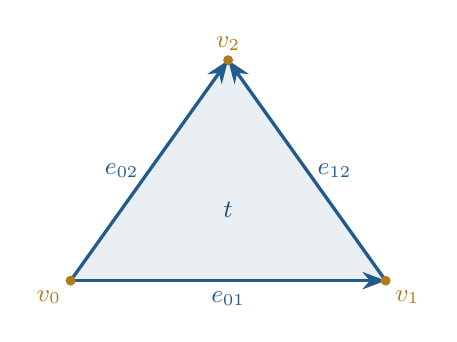
\begin{tikzpicture}[>=Stealth,line cap=round,
  every node/.style={font=\small}]
 \coordinate (v0) at (0,0);
 \coordinate (v1) at (4,0);
 \coordinate (v2) at (2,2.8);
 \fill[manifoldblue!10] (v0)--(v1)--(v2)--cycle;
 \draw[->,very thick,manifoldblue] (v0)--
  node[midway,below] {$e_{01}$} (v1);
 \draw[->,very thick,manifoldblue] (v1)--
  node[midway,right] {$e_{12}$} (v2);
 \draw[->,very thick,manifoldblue] (v0)--
  node[midway,left] {$e_{02}$} (v2);
 \fill[manifoldgold!85!black] (v0) circle (1.8pt)
  node[below left] {$v_0$};
 \fill[manifoldgold!85!black] (v1) circle (1.8pt)
  node[below right] {$v_1$};
 \fill[manifoldgold!85!black] (v2) circle (1.8pt)
  node[above] {$v_2$};
 \node[manifoldblue!80!black] at (2,.9) {$t$};
\end{tikzpicture}
\caption{Wybrane orientacje krawędzi i dwuwymiarowy generator $t$.
Po usunięciu $t$ obwód jest niezerową klasą homologii;
po jego dodaniu staje się brzegiem $\partial_2t$.}
\label{fig:homologia-alg-trojkat}
\end{figure}

\begin{definicja}[Odwzorowanie łańcuchowe]
\index{odwzorowanie lancuchowe@Odwzorowanie łańcuchowe}
\label{def:mapa-lancuchowa}
Odwzorowanie $f:C_\bullet\to D_\bullet$ to rodzina
homomorfizmów $f_n:C_n\to D_n$ zgodnych
z różniczkami:
\begin{equation}\label{eq:mapa-lancuchowa}
 \partial^D_n f_n=f_{n-1}\partial^C_n.
\end{equation}
Oznacza to, że najpierw zastosować $f$,
a potem wziąć brzeg, daje ten sam wynik,
co zrobić to w odwrotnej kolejności.
\end{definicja}

\begin{stwierdzenie}[Odwzorowanie indukowane na homologii]
\label{prop:homologia-funktor}
Odwzorowanie łańcuchowe $f$ wyznacza homomorfizmy
$H_n(f):H_n(C)\to H_n(D)$,
$H_n(f)[z]=[f_n(z)]$. Zachodzą
$H_n(\id_C)=\id_{H_n(C)}$ oraz
$H_n(gf)=H_n(g)H_n(f)$.
\end{stwierdzenie}
\begin{proof}
Jeżeli $\partial^C_n z=0$, to z~\eqref{eq:mapa-lancuchowa}
$\partial^D_n f_nz=f_{n-1}\partial^C_nz=0$, czyli
$f_nz$ jest cyklem. Jeżeli zmienimy
$z$ na $z+\partial^C_{n+1}w$, jego obraz zmieni się o
$f_n(\partial^C_{n+1}w)=\partial^D_{n+1}(f_{n+1}w)$,
czyli o brzeg. Odwzorowanie na klasach jest więc
dobrze określone i liniowe.
Równość dla identyczności to $[\id_C(z)]=[z]$.
Dla złożenia otrzymujemy na dowolnej klasie
$H_n(g\circ f)[z]=[g_n(f_n(z))]
=(H_n(g)\circ H_n(f))[z]$.
\end{proof}

\begin{przyklad}[Odwzorowanie na klasach reszt]
\label{prz:homologia-mapa-mod-m}
Niech $C_\bullet$ będzie dwuwyrazowym kompleksem
$0\to\Z\xrightarrow{\times m}\Z\to0$,
$m\geq2$. Mnożenie przez ustaloną liczbę
całkowitą $k$ w obu stopniach jest odwzorowaniem
łańcuchowym, bo $k(mx)=m(kx)$.
W stopniu $0$ daje ono
$H_0(f):\Z/m\Z\to\Z/m\Z$, $[x]\mapsto[kx]$.
Na przykład dla $m=6$ i $k=2$ obraz składa się
z klas $[0],[2],[4]$, więc odwzorowanie
indukowane nie jest surjekcją. Dwa różne
odwzorowania łańcuchowe dla $k$ i $k+m$
dają jednak to samo odwzorowanie na $H_0$.
Homologia zachowuje więc część informacji
o odwzorowaniu, ale nie całą jego postać.
\end{przyklad}

\section{Skąd bierze się długi ciąg dokładny homologii?}
\label{sec:dlugi-ciag-homologii}

Niech $A_\bullet,B_\bullet,C_\bullet$ będą
kompleksami, a $i:A_\bullet\to B_\bullet$,
$p:B_\bullet\to C_\bullet$ odwzorowaniami łańcuchowymi.
Mówimy, że
\[
 0\longrightarrow A_\bullet
 \xrightarrow{i}B_\bullet
 \xrightarrow{p}C_\bullet
 \longrightarrow0
\]
jest \emph{krótkim ciągiem dokładnym kompleksów},
jeśli dla \emph{każdego} $n$ ciąg modułów
\begin{equation}\label{eq:ses-kompleks}
 0\longrightarrow A_n\xrightarrow{i_n}B_n
 \xrightarrow{p_n}C_n\longrightarrow0
\end{equation}
jest dokładny. Stopniowa dokładność nie
mówi jeszcze, że ciąg powstałych homologii
jest krótki i dokładny: cykl podniesiony
z $C_n$ może przestać być cyklem w $B_n$.
Jego brzeg mierzy właśnie tę przeszkodę.
Ponieważ $c$ jest cyklem, brzeg podniesienia
ma zerowy obraz w $C_{n-1}$, zatem leży
w $i_{n-1}(A_{n-1})$. Po odczytaniu go w $A$
otrzymamy cykl stopnia o jeden niższego.
To wyjaśnia zarówno pochodzenie, jak i stopień
odwzorowania łączącego na Rysunku~\ref{fig:homologia-delta}.

\begin{figure}[!htbp]
\centering
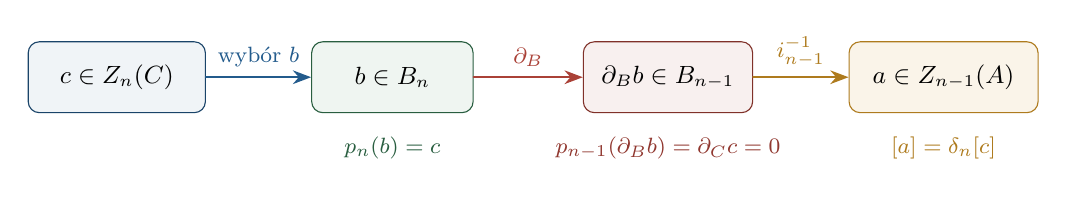
\begin{tikzpicture}[>=Stealth,line cap=round,
  every node/.style={font=\small}]
 \node[draw=manifoldblue!75!black,rounded corners,
  fill=manifoldblue!7,minimum width=2.25cm,
  minimum height=.9cm] (c) at (-5.25,0) {$c\in Z_n(C)$};
 \node[draw=manifoldgreen!75!black,rounded corners,
  fill=manifoldgreen!8,minimum width=2.05cm,
  minimum height=.9cm] (b) at (-1.75,0) {$b\in B_n$};
 \node[draw=manifoldred!75!black,rounded corners,
  fill=manifoldred!8,minimum width=2.15cm,
  minimum height=.9cm] (db) at (1.75,0) {$\partial_Bb\in B_{n-1}$};
 \node[draw=manifoldgold!85!black,rounded corners,
  fill=manifoldgold!10,minimum width=2.4cm,
  minimum height=.9cm] (a) at (5.25,0) {$a\in Z_{n-1}(A)$};
 \draw[->,thick,manifoldblue] (c) --
  node[midway,above,font=\footnotesize] {wybór $b$} (b);
 \draw[->,thick,manifoldred] (b) --
  node[midway,above,font=\footnotesize] {$\partial_B$} (db);
 \draw[->,thick,manifoldgold!85!black] (db) --
  node[midway,above,font=\footnotesize] {$i_{n-1}^{-1}$} (a);
 \node[font=\footnotesize,manifoldgreen!75!black]
  at (-1.75,-.9) {$p_n(b)=c$};
 \node[font=\footnotesize,manifoldred!85!black]
  at (1.75,-.9) {$p_{n-1}(\partial_Bb)=\partial_Cc=0$};
 \node[font=\footnotesize,manifoldgold!85!black]
  at (5.25,-.9) {$[a]=\delta_n[c]$};
\end{tikzpicture}
\caption{Odwzorowanie łączące: podnosimy cykl $c$, bierzemy brzeg
podniesienia $b$, po czym odczytujemy go w $A_{n-1}$.
Odwrócenie $i_{n-1}$ dotyczy tylko jego obrazu
$\ker p_{n-1}$; całego odwzorowania $i_{n-1}$ nie odwracamy.}
\label{fig:homologia-delta}
\end{figure}

\noindent\emph{Porównanie w Bibliotece matematycznej:} \atlasref{TOP-03::thm:les-homologia}{TOP-03: długi ciąg dokładny homologii}.

\begin{twierdzenie}[Długi ciąg dokładny]
\label{thm:les-homologia}
Z krótkiego ciągu dokładnego kompleksów
otrzymujemy naturalny długi ciąg dokładny
\begin{equation}\label{eq:les-homologia}
 \cdots\longrightarrow H_n(A)
 \xrightarrow{i_*}H_n(B)
 \xrightarrow{p_*}H_n(C)
 \xrightarrow{\delta_n}H_{n-1}(A)
 \xrightarrow{i_*}H_{n-1}(B)
 \longrightarrow\cdots.
\end{equation}
Odwzorowanie \emph{łączące} $\delta_n$ ma następujący
konkretny wzór. Dla cyklu $c\in C_n$ wybieramy
podniesienie $b\in B_n$ z $p_n(b)=c$.
Wtedy $\partial_B b=i_{n-1}(a)$ dla dokładnie
jednego $a\in A_{n-1}$, a
\begin{equation}\label{eq:delta-wzor}
 \delta_n[c]=[a]\in H_{n-1}(A).
\end{equation}
Jeżeli kompleksy są zerowe w ujemnych stopniach,
końcowy fragment ma postać
$H_0(A)\to H_0(B)\to H_0(C)\to0$.
\end{twierdzenie}
\begin{proof}
\emph{Konstrukcja i cykl.} Surjektywność $p_n$
daje podniesienie $b$. Ponieważ $p$ jest odwzorowaniem
łańcuchowym, $p_{n-1}(\partial_Bb)=\partial_C(p_nb)
=\partial_Cc=0$.
Z dokładności~\eqref{eq:ses-kompleks} w
stopniu $n-1$ mamy
$\partial_Bb\in\ker p_{n-1}=\operatorname{im}i_{n-1}$,
więc istnieje $a$ z $i_{n-1}a=\partial_Bb$.
Iniektywność $i_{n-1}$ daje jego jednoznaczność.
W tym miejscu $i_{n-1}^{-1}$ oznacza odwrotność
tylko na podmodule $\operatorname{im}i_{n-1}$.
Ponadto $i_{n-2}(\partial_Aa)
=\partial_B(i_{n-1}a)=\partial_B^2b=0$.
Iniektywność $i_{n-2}$ wymusza $\partial_Aa=0$.
Możemy więc wziąć klasę $[a]$.

\emph{Niezależność od podniesienia.} Jeśli $b'$ też
podnosi $c$, to $b'-b=i_n(u)$ dla pewnego
$u\in A_n$. Wtedy $\partial_Bb'=\partial_Bb
+\partial_Bi_nu=i_{n-1}(a+\partial_Au)$.
Nowy cykl w $A$ różni się od $a$ o brzeg,
więc wyznacza tę samą klasę.

\emph{Niezależność od reprezentanta.}
Niech $c'=c+\partial_Cv$, $v\in C_{n+1}$.
Wybierzmy podniesienie $w\in B_{n+1}$ elementu $v$.
Wtedy $b+\partial_Bw$ podnosi $c'$ i ma ten sam
brzeg co $b$, bo $\partial_B^2w=0$.
Każde inne podniesienie $c'$ różni się od tego
o element $\operatorname{im}i_n$; właśnie
sprawdzona niezależność od podniesienia
kończy dowód niezależności od wyboru reprezentanta klasy $[c]$.
Suma podniesień podnosi sumę cykli, a
podniesienie $rb$ podnosi $rc$, więc $\delta_n$
jest homomorfizmem $R$-modułów.

\emph{Dokładność przy $H_n(B)$.}
Z $pi=0$ mamy $p_*i_*=0$.
Jeśli $[b]\in H_n(B)$ spełnia
$p_*[b]=0$, to dla cyklu $b$
istnieje $v\in C_{n+1}$ z
$p_nb=\partial_Cv$. Wybierzmy podniesienie
$w\in B_{n+1}$ elementu $v$.
Wtedy $b'=b-\partial_Bw$ nadal jest cyklem,
$[b']=[b]$ i
$p_nb'=p_nb-\partial_Cv=0$. Z dokładności
w stopniu $n$ mamy $b'=i_na$.
Ponieważ $\partial_Bb'=i_{n-1}\partial_Aa=0$
i $i_{n-1}$ jest iniektywna, $a$ jest
cyklem. Stąd $[b]=i_*[a]$.

\emph{Dokładność przy $H_n(C)$.}
Jeżeli $c=p_nb$ dla cyklu $b$, możemy
w definicji $\delta_n$ wybrać to właśnie
podniesienie: $\partial_Bb=0$, więc $\delta_n[c]=0$.
Odwrotnie, załóżmy $\delta_n[c]=0$
i podnieśmy cykl $c$ do $b$.
Jeśli $\partial_Bb=i_{n-1}a$, to $[a]=0$,
czyli $a=\partial_Au$ dla pewnego $u\in A_n$.
Element $b-i_nu$ jest cyklem, bo
$\partial_B(b-i_nu)=i_{n-1}(a-\partial_Au)=0$,
a $p_n(b-i_nu)=c$. Zatem
$[c]=p_*[b-i_nu]$.

\emph{Dokładność przy $H_{n-1}(A)$.}
Dla klasy $\delta_n[c]=[a]$ mamy
$i_{n-1}a=\partial_Bb$, czyli $i_*[a]=0$.
Odwrotnie, jeżeli $a\in Z_{n-1}(A)$
i $i_*[a]=0$, istnieje $b\in B_n$
takie, że $i_{n-1}a=\partial_Bb$.
Wówczas $c=p_nb$ jest cyklem, bo
$\partial_Cc=p_{n-1}\partial_Bb=p_{n-1}i_{n-1}a=0$,
a wzór~\eqref{eq:delta-wzor} daje
$\delta_n[c]=[a]$.
Przesuwając indeks $n$ o jeden,
obejmujemy tymi trzema sprawdzeniami
każde miejsce całego ciągu~\eqref{eq:les-homologia}.
W końcu, przy założonej zerowości kompleksów w ujemnych
stopniach mamy $A_{-1}=0$, a więc
$H_{-1}(A)=0$, więc $H_0(B)\to H_0(C)$
jest surjekcją na mocy właśnie wykazanej
dokładności.
\end{proof}

\begin{uwaga}[Naturalność odwzorowania łączącego]
\label{uwaga:les-naturalnosc}
Jeżeli mamy odwzorowanie między dwoma krótkimi
ciągami kompleksów, zgodne z $i,p$ i
różniczkami, to odwzorowania na homologiach
komutują także z $\delta$.
Dokładniej, są to odwzorowania łańcuchowe
$f_A:A\to A'$, $f_B:B\to B'$, $f_C:C\to C'$ spełniające
$f_Bi=i'f_A$ oraz $p'f_B=f_Cp$.
Istotnie, podniesienie $b$ cyklu $c$ przechodzi
w podniesienie obrazu $c$, jego brzeg przechodzi
w obraz $\partial_Bb$, a wstrzyknięcie $i$
pozwala odczytać obraz tego samego $a$:
z $i_{n-1}a=\partial_Bb$ wynika
$i'_{n-1}f_{A,n-1}a=\partial_{B'}f_{B,n}b$.
Iniektywność $i'_{n-1}$ identyfikuje więc
cykl użyty do obliczenia $\delta'_n$ z $f_{A,n-1}a$.
Równość na reprezentantach ma postać
$\delta'_n(H_n(f_C)[c])
=H_{n-1}(f_A)(\delta_n[c])$.
\end{uwaga}

\begin{przyklad}[Odwzorowanie łączące jako mnożenie przez $m$]
\label{prz:delta-razy-m}
Ustalmy $m\geq2$ i pracujmy nad $\Z$.
Niech $A_\bullet$ ma jedyny niezerowy moduł
$A_0=\Z$, a $C_\bullet$ jedyny niezerowy
moduł $C_1=\Z$. Niech $B_\bullet$ ma
$B_1=B_0=\Z$ i różniczkę
$\partial_B=\times m:B_1\to B_0$.
W stopniu $0$ odwzorowanie $i_0:A_0\to B_0$
jest identycznością, a w stopniu $1$
odwzorowanie $p_1:B_1\to C_1$ jest identycznością;
pozostałe odwzorowania to jedyne możliwe odwzorowania zerowe.
W każdym stopniu otrzymujemy rozszczepiony
krótki ciąg dokładny modułów. Mamy natomiast
$H_1(B)=0$ i $H_0(B)=\Z/m\Z$.
Cykl $c=1\in C_1$ podnosimy do $b=1\in B_1$.
Jego brzeg to $m=i_0(m)\in B_0$,
więc $\delta_1:\Z\to\Z$ jest mnożeniem przez $m$.
Fragment długiego ciągu staje się dokładnie
ciągiem $0\to\Z\xrightarrow{\times m}\Z
\to\Z/m\Z\to0$ z Przykładu~\ref{prz:ses-mod-m}.
Gdyby istniał przekrój $s:C_\bullet\to B_\bullet$
złożony z odwzorowań łańcuchowych, w stopniu $1$
musiałoby być $s_1=\id_{\Z}$, bo $p_1=\id_{\Z}$.
Wówczas jednak $\partial_Bs_1=\times m\ne0$,
podczas gdy $s_0\partial_C=0$.
Stopniowe rozszczepienie nie daje zatem
rozszczepienia kompleksów.
\end{przyklad}
\section{Kohomologia algebraiczna i jej długi ciąg}
\label{sec:kohomologia-algebraiczna}

W homologii różniczka obniża stopień.
Kohomologia powstaje z równie prostej
konstrukcji, w której różniczka stopień
\emph{podwyższa}. Gdy elementy kompleksu
łańcuchowego są wektorami, elementy
kompleksu dualnego są funkcjonałami:
zamiast brać brzeg wektora, oceniamy
funkcjonał na brzegu.

\begin{definicja}[Kompleks kołańcuchowy i kohomologia]
\index{kompleks kołańcuchowy i kohomologia@Kompleks kołańcuchowy i kohomologia}
\label{def:kohomologia-algebraiczna}
\emph{Kompleks kołańcuchowy} $K^\bullet$ to
moduły $K^n$ i homomorfizmy
$d^n:K^n\to K^{n+1}$ z
$d^{n+1}d^n=0$ dla $n\in\Z$. Jego \emph{kohomologią stopnia $n$}
jest
\begin{equation}\label{eq:kohomologia-def}
 H^n(K):=\frac{\ker(d^n:K^n\to K^{n+1})}
 {\operatorname{im}(d^{n-1}:K^{n-1}\to K^n)}.
\end{equation}
Elementy jądra nazywamy \emph{kocyklami},
a elementy obrazu \emph{kobrzegami}.
Odwzorowanie kołańcuchowe $F:K^\bullet\to L^\bullet$
składa się z $F^n:K^n\to L^n$ spełniających
$d_L^nF^n=F^{n+1}d_K^n$.
\end{definicja}

Tak jak w dowodzie
Stwierdzenia~\ref{prop:homologia-funktor},
odwzorowanie kołańcuchowe przenosi kocykle w
kocykle i kobrzegi w kobrzegi:
$d_LFz=Fdz=0$ oraz
$F(d_Ku)=d_L(Fu)$. Wobec tego definiuje
$H^n(F)[z]=[F^nz]$. Równość
$H^n(K)=0$ mówi dokładnie, że
$K^{n-1}\to K^n\to K^{n+1}$
jest dokładny w $K^n$.

\begin{przyklad}[Kohomologia dwuwyrazowego kompleksu]
Dla $K^0=K^1=\Z$, $d^0=\times2$
i wszystkich innych modułów równych $0$
otrzymujemy $H^0(K)=0$ oraz
$H^1(K)=\Z/2\Z$. W stopniu $1$ nie ma
już różniczki wychodzącej, więc
wszystkie elementy $\Z$ są kocyklami;
kobrzegami są liczby parzyste.
\end{przyklad}

\begin{stwierdzenie}[Kompleks dualny]
\label{prop:kompleks-dualny}
Dla kompleksu łańcuchowego $C_\bullet$
i $R$-modułu $G$ połóżmy
$C^n(C;G):=\operatorname{Hom}_R(C_n,G)$ oraz
$d^n\varphi:=\varphi\circ\partial_{n+1}$.
Wtedy $C^\bullet(C;G)$ jest kompleksem
kołańcuchowym. Odwzorowanie łańcuchowe
$f:C_\bullet\to D_\bullet$ daje odwzorowanie
kołańcuchowe w odwrotną stronę,
$f^*:C^\bullet(D;G)\to C^\bullet(C;G)$,
$f^*(\varphi)=\varphi\circ f_n$.
\end{stwierdzenie}
\begin{proof}
Dla $\varphi:C_n\to G$ mamy
$d^{n+1}(d^n\varphi)
=\varphi\circ(\partial_{n+1}\partial_{n+2})=0$.
Z kolei dla $\varphi:D_n\to G$
oraz $x\in C_{n+1}$ równość odwzorowań łańcuchowych
z~\eqref{eq:mapa-lancuchowa} daje
\[
 (d f^*\varphi)(x)
 =\varphi(f_n(\partial_C x))
 =\varphi(\partial_D(f_{n+1}x))
 =(f^*d\varphi)(x).
\]
To dowodzi zgodności z różniczką.
Odwrócenie kierunku jest widoczne już w typach:
funkcjonał na $D_n$ po złożeniu z $f_n:C_n\to D_n$
staje się funkcjonałem na $C_n$.
\end{proof}

Słowo \emph{dualny} wymaga tu ostrożności:
zastosowanie $\operatorname{Hom}_R(-,G)$
do krótkiego ciągu dokładnego modułów
nie musi dać krótkiego ciągu dokładnego.
Na przykład przy $G=\Z$ w ciągu
$0\to2\Z\hookrightarrow\Z\to\Z/2\Z\to0$
funkcjonał $2\Z\to\Z$, $2k\mapsto k$,
nie przedłuża się do homomorfizmu
$\Z\to\Z$: musiałby wysłać $1$
na liczbę $t$ z $2t=1$.
Z tego powodu nie będziemy budować
długiego ciągu kohomologii przez
bezrefleksyjne dualizowanie
Twierdzenia~\ref{thm:les-homologia}.

\begin{twierdzenie}[Długi ciąg kohomologii]
\label{thm:les-kohomologia}
Jeżeli w każdym stopniu dokładny jest
krótki ciąg \emph{kompleksów kołańcuchowych}
\[
 0\longrightarrow A^\bullet\xrightarrow{i}B^\bullet
 \xrightarrow{p}C^\bullet\longrightarrow0,
\]
to istnieje długi ciąg dokładny
\begin{equation}\label{eq:les-kohomologia}
 \cdots\longrightarrow H^n(A)
 \xrightarrow{i_*}H^n(B)
 \xrightarrow{p_*}H^n(C)
 \xrightarrow{\delta^n}H^{n+1}(A)
 \xrightarrow{i_*}H^{n+1}(B)\longrightarrow\cdots.
\end{equation}
\end{twierdzenie}
\begin{proof}
Dla kocyklu $c\in C^n$ wybierzmy podniesienie
$b\in B^n$ z $p(b)=c$.
Wtedy $p(d_Bb)=d_Cc=0$, więc dokładność
w stopniu $n+1$ i iniektywność $i$
dają dokładnie jedno $a\in A^{n+1}$
z $i(a)=d_Bb$.
Ponieważ $i(d_Aa)=d_B^2b=0$,
otrzymujemy kocykl $a$.
Definiujemy $\delta^n[c]=[a]$.
Jeśli podniesienie $b$ zastąpimy $b+i(u)$,
to $a$ zmienia się na $a+d_Au$.
Jeśli $c$ zastąpimy $c+d_Cv$, to po
wyborze podniesienia $w$ dla $v$ możemy
zastąpić $b$ przez $b+d_Bw$,
co w ogóle nie zmienia $d_Bb$.
Oba wybory prowadzą zatem do tej
samej klasy. Podniesienie sumy można wziąć
jako sumę podniesień, a $rb$ podnosi $rc$ dla $r\in R$.
Zatem $\delta^n$ jest $R$-liniowa.

Sprawdźmy każde z trzech rodzajów miejsc
w~\eqref{eq:les-kohomologia}.
Przy $H^n(B)$ mamy $p_*i_*=0$.
Jeśli $b\in B^n$ jest kocyklem
i $p_*[b]=0$, to $p(b)=d_Cv$
dla pewnego $v\in C^{n-1}$.
Podnieśmy $v$ do $w\in B^{n-1}$.
Wówczas $b-d_Bw$ jest kocyklem
z tą samą klasą co $b$, a jego
obraz przez $p$ wynosi $0$.
Równa się więc $i(a)$ dla pewnego
$a\in A^n$. Z $0=d_Bi(a)=i(d_Aa)$
i iniektywności $i$ dostajemy
$d_Aa=0$, a zatem $[b]=i_*[a]$.

Przy $H^n(C)$ inkluzja
$\operatorname{im}p_*\subseteq\ker\delta^n$
wynika z wybrania jako podniesienia $c=p(b)$
samego kocyklu $b$: jego różniczka jest $0$.
Jeśli odwrotnie $\delta^n[c]=0$,
to dla podniesienia $b$ mamy $d_Bb=i(a)$,
gdzie $a=d_Au$ dla pewnego $u\in A^n$.
Element $b-i(u)$ jest kocyklem,
którego obraz to $c$, więc
$[c]\in\operatorname{im}p_*$.

Przy $H^{n+1}(A)$ element
$i_*\delta^n[c]$ reprezentuje
$i(a)=d_Bb$ i dlatego jest zerowy.
Jeśli z drugiej strony $a\in A^{n+1}$
jest kocyklem i $i_*[a]=0$,
to $i(a)=d_Bb$ dla pewnego
$b\in B^n$. Obraz $c=p(b)$ jest
kocyklem, gdyż $d_Cc=p(d_Bb)=p(i(a))=0$,
a jego odwzorowanie łączące wynosi $[a]$.
Zmiana $n$ daje dokładność także
w pozostałych stopniach. Konstrukcja jest naturalna:
dla zgodnych odwzorowań $f_A,f_B,f_C$ między krótkimi ciągami
podniesieniem $f_C(c)$ jest $f_B(b)$, a jego różniczka to
$f_B(d_Bb)=f_B(i(a))=i'(f_A(a))$.
Stąd $\delta'^n H^n(f_C)=H^{n+1}(f_A)\delta^n$.
\end{proof}

\begin{przyklad}[Niezerowe odwzorowanie łączące w kohomologii]
Niech $B^0=B^1=\Z$, $d_B^0=\times2$, a inne
wyrazy $B$ będą zerowe. Weźmy podkompleks
$A^1=B^1=\Z$, $A^0=0$; iloraz $C=B/A$
ma jedyny niezerowy wyraz $C^0=\Z$.
W krótkim ciągu $0\to A\to B\to C\to0$
klasę $k\in H^0(C)=\Z$ podnosimy do $k\in B^0$.
Jej różniczka wynosi $2k\in B^1=A^1$, zatem
$\delta^0:H^0(C)\to H^1(A)$ jest mnożeniem przez $2$.
Dokładność fragmentu
$0\to\Z\xrightarrow{\times2}\Z\to\Z/2\Z\to0$
odtwarza $H^0(B)=0$ i $H^1(B)=\Z/2\Z$.
Przykład pokazuje, że różniczka podniesienia mierzy
przeszkodę w podniesieniu \emph{kocyklu} do kocyklu.
\end{przyklad}

\begin{twierdzenie}[Nad ciałem kohomologia jest dualna do homologii]
\label{thm:field-hom-dual}
Niech $C_\bullet$ będzie kompleksem
przestrzeni liniowych nad ciałem
$\mathbb K$, a
$C^n=\operatorname{Hom}_{\mathbb K}(C_n,\mathbb K)$.
Wtedy naturalne przypisanie
\begin{equation}\label{eq:field-duality}
 H^n(C^\bullet)
 \longrightarrow\operatorname{Hom}_{\mathbb K}
  (H_n(C_\bullet),\mathbb K),
 \qquad [\varphi]\longmapsto
     ([z]\longmapsto\varphi(z))
\end{equation}
jest izomorfizmem. Zakładamy, że
przestrzenie pozwalają na wybór
dopełnień podprzestrzeni
(w szczególności wystarcza skończony wymiar).
\end{twierdzenie}
\begin{proof}
Chodzi o dualność \emph{algebraiczną}: rozważamy wszystkie
funkcjonały liniowe, bez założeń topologicznych.
Jeżeli $\varphi\in C^n$ jest kocyklem,
to $d^n\varphi=\varphi \partial_{n+1}=0$.
Zatem $\varphi$ znika na $B_n$,
więc jej wartość na $z\in Z_n$
zależy tylko od klasy $[z]\in H_n$.
Jeżeli zmienimy $\varphi$ na
$\varphi+d^{n-1}\psi
=\varphi+\psi \partial_n$, to dla cyklu $z$
mamy $\partial_nz=0$, więc otrzymujemy
ten sam funkcjonał na $H_n$.
Odwzorowanie~\eqref{eq:field-duality} jest
dobrze określone i liniowe. Jest też naturalne: dla odwzorowania
łańcuchowego $f:C\to D$, kocyklu $\varphi$ na $D$ i cyklu $z$ na $C$
mamy $(f^*\varphi)(z)=\varphi(fz)$. Zatem obie drogi, przez
$H^n(f^*)$ lub przez prekompozycję z $H_n(f)$, dają ten sam funkcjonał.

Aby pokazać surjektywność, weźmy
$\ell:H_n=Z_n/B_n\to\mathbb K$.
Złożenie $Z_n\to H_n\xrightarrow{\ell}\mathbb K$
jest liniowe i znika na $B_n$.
Wybieramy dopełnienie $Z_n$ w $C_n$
i przedłużamy funkcjonał liniowo
na $C_n$, na przykład jako zero
na tym dopełnieniu. Otrzymany
$\varphi$ spełnia
$\varphi \partial_{n+1}=0$, bo
$\operatorname{im}\partial_{n+1}=B_n$;
jest kocyklem wysyłanym na $\ell$.

Jeżeli klasa $[\varphi]$ trafia na zero,
to $\varphi$ znika na całym $Z_n$.
Możemy więc zdefiniować funkcjonał
$\eta$ na $B_{n-1}=\operatorname{im}\partial_n$
przez $\eta(\partial_nx)=\varphi(x)$.
Jest dobrze określony: z
$\partial_nx=\partial_nx'$ wynika $x-x'\in Z_n$,
a tam $\varphi$ znika.
Wybieramy dopełnienie $B_{n-1}$
w $C_{n-1}$ i przedłużamy $\eta$
do $\psi:C_{n-1}\to\mathbb K$.
Wtedy $\varphi=\psi \partial_n=d^{n-1}\psi$
jest kobrzegiem. Jądro odwzorowania
w~\eqref{eq:field-duality} jest więc zerowe.
\end{proof}

\begin{uwaga}[Dlaczego ważne są współczynniki?]
Nad $\Z$ odpowiednik~\eqref{eq:field-duality}
może być fałszywy. Dla kompleksu
$C_1=C_0=\Z$ z $\partial_1=\times2$ mamy
$H_0(C)=\Z/2$ i $H_1(C)=0$,
podczas gdy dla dualnego kompleksu
$H^1(C^\bullet)=\Z/2$.
Grupa $\operatorname{Hom}_{\Z}
(H_1(C),\Z)$ jest zerowa.
Ta dodatkowa klasa kohomologii
wykrywa informację torsyjną z
poprzedniego stopnia. Nie utożsamiamy
więc homologii z kohomologią bez
sprawdzenia założeń o współczynnikach.
\end{uwaga}
\section{Homotopia łańcuchowa i uproszczenia kompleksów}
\label{sec:homotopia-lancuchowa}

Jedna homologia może mieć bardzo różne opisy
przez generatory i różniczki. Poniższe kryterium
mówi, kiedy dwa odwzorowania kompleksów dają
\emph{dokładnie to samo} odwzorowanie na
homologiach. Jest to algebraiczny mechanizm
usuwania par generatorów, które wzajemnie
się kasują.

\begin{definicja}[Homotopia łańcuchowa]
\index{homotopia lancuchowa@Homotopia łańcuchowa}
\label{def:homotopia-lancuchowa}
Dwa odwzorowania łańcuchowe $f,g:C_\bullet\to D_\bullet$
są \emph{łańcuchowo homotopijne}, jeśli istnieją
homomorfizmy $R$-modułów $h_n:C_n\to D_{n+1}$ takie, że
\begin{equation}\label{eq:chain-homotopy}
 f_n-g_n=\partial^D_{n+1}h_n+h_{n-1}\partial^C_n
 \qquad\text{dla każdego }n.
\end{equation}
Kompleks $C_\bullet$ jest \emph{ściągalny},
jeśli $\id_C$ jest łańcuchowo homotopijna
z odwzorowaniem zerowym.
\end{definicja}

Wzór~\eqref{eq:chain-homotopy} przypomina
zasadę całkowania przez części: różnica
odwzorowań składa się z dwóch operacji, w których
$h$ i $\partial$ występują w przeciwnych
kolejnościach. Na cyklach drugi składnik
znika, a pierwszy jest brzegiem. Homotopia $h$
podnosi stopień o jeden; nie musi sama komutować
z różniczką, bo mierzy różnicę między $f$ i $g$.

\begin{twierdzenie}[Homotopia nie zmienia homologii]
\label{thm:homotopia-homologia}
Jeśli $f$ i $g$ są łańcuchowo homotopijne,
to $H_n(f)=H_n(g)$ dla każdego $n$.
W szczególności kompleks ściągalny jest
acykliczny. Jeśli istnieją odwzorowania łańcuchowe
$f:C_\bullet\to D_\bullet$ i
$g:D_\bullet\to C_\bullet$ z
$gf\simeq\id_C$ i $fg\simeq\id_D$,
to $H_n(f)$ i $H_n(g)$ są wzajemnymi
izomorfizmami.
\end{twierdzenie}
\begin{proof}
Dla $z\in Z_n(C)$ równanie~\eqref{eq:chain-homotopy}
redukuje się do
$f_n(z)-g_n(z)=\partial^D_{n+1}h_n(z)$,
bo $\partial^C_nz=0$. Różnica obrazów jest
brzegiem, więc $[f_n(z)]=[g_n(z)]$.
Gdy $f=\id_C$, $g=0$, otrzymujemy
$[z]=[0]$ dla każdej klasy, czyli
$H_n(C)=0$.
Na koniec, dzięki Stwierdzeniu~\ref{prop:homologia-funktor},
$H_n(g)H_n(f)=H_n(gf)=H_n(\id_C)=\id$ oraz
$H_n(f)H_n(g)=\id$.
Stąd oba odwzorowania na homologiach są
odwrotne do siebie.
\end{proof}

\begin{przyklad}[Najprostsze ściągnięcie]
Dla kompleksu
$0\to R\xrightarrow{\id}R\to0$
z modułami w stopniach $1$ i $0$
połóżmy $h_0:R=C_0\to C_1=R$
równe identyczności, a pozostałe
$h_n=0$. W stopniu $0$ mamy
$\partial_1h_0=\id_{C_0}$, a w stopniu
$1$ mamy $h_0\partial_1=\id_{C_1}$.
Wzór~\eqref{eq:chain-homotopy}
daje $\id_C=\partial h+h\partial$.
\end{przyklad}

\begin{twierdzenie}[Algebraiczne skasowanie pary generatorów]
\label{thm:kasowanie-pary}
Niech $C_\bullet$ będzie kompleksem
wolnych $R$-modułów z ustalonymi
bazami, a $n\geq1$. Załóżmy, że
przy generatorze $f\in C_{n-1}$
we współrzędnych $\partial_n(e)$ dla pewnego
generatora $e\in C_n$ stoi skalar
odwracalny $u\in R$.
Wtedy przez zmiany baz można rozłożyć
$C_\bullet$ na sumę prostą
podkompleksu i dwuwyrazowego kompleksu
\[
 0\longrightarrow R e
 \xrightarrow{\ \partial_n\ }R\,\partial_n(e)
 \longrightarrow0,
\]
w którym $\partial_n$ jest izomorfizmem.
Usunięcie tej pary nie zmienia homologii.
\end{twierdzenie}
\begin{proof}
Zapiszmy
$C_n=R e\oplus M$ oraz
$C_{n-1}=R f\oplus N$, gdzie
$M,N$ są rozpięte przez pozostałe
wybrane wektory bazowe.
Z założenia
$\partial_n(e)=u f+v$ z $v\in N$.
Ponieważ $u$ jest odwracalny,
$f':=\partial_n(e)$ może zastąpić $f$
w bazie $C_{n-1}$:
$C_{n-1}=R f'\oplus N$.
Rzeczywiście, $f=u^{-1}(f'-v)$
pozwala przejść w obie strony
między rozkładami.

Dla $x\in M$ zapiszmy
$\partial_n(x)=a(x)f+w(x)$,
gdzie $a(x)\in R$ i $w(x)\in N$.
Zmieńmy też bazę w stopniu $n$,
zastępując każdy bazowy $x\in M$
wektorem $x':=x-u^{-1}a(x)e$.
Wtedy
\[
 \partial_n(x')
 =a(x)f+w(x)-u^{-1}a(x)(uf+v)
 =w(x)-u^{-1}a(x)v\in N.
\]
Nowe wektory $x'$ razem z $e$
tworzą bazę $C_n$: możemy odzyskać
$x=x'+u^{-1}a(x)e$.
Oznaczmy ich rozpiętość przez $M'$.
Mamy zatem $\partial_n(Re)=Rf'$
i $\partial_n(M')\subseteq N$.

Równość $\partial_{n-1}(f')=\partial_{n-1}\partial_n(e)=0$
mówi, że z $Rf'$ nie wychodzi
różniczka. Z kolei dla $y\in C_{n+1}$
zapiszmy $\partial_{n+1}(y)=t e+x'$,
$x'\in M'$. Po zastosowaniu $\partial_n$
dostajemy
$0=\partial_n\partial_{n+1}(y)=t f'+\partial_n(x')$.
Pierwszy składnik należy do $Rf'$,
drugi do $N$; rozkład jest prosty,
więc $t=0$. Żadna różniczka
z wyższego stopnia nie trafia do $Re$.
Pozostałe moduły wraz z $M'$ i $N$
tworzą więc podkompleks, a
$Re\xrightarrow{\cong}Rf'$
jest jego prostym składnikiem
w całym kompleksie.

Na tym dwuwyrazowym składniku
homotopia $h_{n-1}(f')=e$,
zerowa w innych stopniach,
spełnia $\id=\partial h+h\partial$.
Jest on ściągalny. Przedłużmy tę homotopię przez zero na
pozostałym podkompleksie $D$. Dla rzutu $p:C\to D$ i inkluzji
$j:D\to C$ otrzymujemy $pj=\id_D$ oraz
$\id_C-jp=\partial h+h\partial$. Rzut i inkluzja
wyznaczają odwrotne izomorfizmy
na homologiach na mocy
Twierdzenia~\ref{thm:homotopia-homologia}.
\end{proof}

\begin{przyklad}[Skasowanie pary w macierzy różniczki]
Niech $C_1=\Z e\oplus\Z x$ i
$C_0=\Z f\oplus\Z g$, a inne wyrazy będą zerowe.
Zadajmy $\partial_1e=f+3g$ i
$\partial_1x=2f+8g$. W tych bazach macierz różniczki
ma postać $\bigl(\begin{smallmatrix}1&2\\3&8\end{smallmatrix}\bigr)$.
Współczynnik przy $f$ w $\partial_1e$ jest jednostką.
Po zmianach $f'=f+3g$ oraz $x'=x-2e$ otrzymujemy
$\partial_1e=f'$ i
$\partial_1x'=(2f+8g)-2(f+3g)=2g$.
Możemy prześledzić również zmiany macierzy.
Kolumny nowych baz w starych współrzędnych to
$P=\bigl(\begin{smallmatrix}1&0\\3&1\end{smallmatrix}\bigr)$
w stopniu $0$ i
$Q=\bigl(\begin{smallmatrix}1&-2\\0&1\end{smallmatrix}\bigr)$
w stopniu $1$.
Jeśli $D$ jest starą macierzą różniczki, nowa wynosi
\[
 P^{-1}DQ
 =\begin{pmatrix}1&2\\0&2\end{pmatrix}
  \begin{pmatrix}1&-2\\0&1\end{pmatrix}
 =\begin{pmatrix}1&0\\0&2\end{pmatrix}.
\]
Pierwszy czynnik po znaku równości to $P^{-1}D$:
od drugiego wiersza $D$ odejmujemy trzykrotność pierwszego.
Cały kompleks jest więc sumą pary ściągalnej
$\Z e\xrightarrow{\cong}\Z f'$ oraz kompleksu
$\Z x'\xrightarrow{\times2}\Z g$.
Pierwszą parę usuwamy, a druga zachowuje
$H_0(C)=\Z/2\Z$. Sama obecność jednostki w jednym
współczynniku nie usuwa torsji z reszty kompleksu.
\end{przyklad}

Nad $\Z$ jednostkami są tylko $1$ i $-1$.
Współczynnik $2$ w różniczce
$\Z\xrightarrow{\times2}\Z$ nie pozwala
wykonać takiego skasowania: pozostała
klasa $\Z/2$ z
Przykładu~\ref{prz:homologia-rachunki}
jest rzeczywistą przeszkodą.

\begin{stwierdzenie}[Acykliczny kompleks przestrzeni liniowych]
\label{prop:acykliczny-sciagalny}
Jeżeli $C_\bullet$ jest kompleksem
przestrzeni liniowych nad ciałem
$\mathbb K$ i $H_n(C)=0$ dla wszystkich
$n$, to $C_\bullet$ jest ściągalny.
Wystarczy, aby każda podprzestrzeń
$Z_n(C)\subseteq C_n$ miała dopełnienie;
warunek ten zachodzi zawsze przy
skończonych wymiarach.
\end{stwierdzenie}
\begin{proof}
Acykliczność daje $Z_n=B_n$.
Wybierzmy dopełnienie $S_n$ tak, aby
$C_n=Z_n\oplus S_n$. Ograniczenie
$\partial_n|_{S_n}:S_n\to Z_{n-1}$
jest iniektywne: element jego jądra
należy do $S_n\cap Z_n=\{0\}$.
Jest też surjektywne, bo
$\partial_n(C_n)=B_{n-1}=Z_{n-1}$
i $\partial_n$ znika na $Z_n$.
Ma więc odwrotność.
Każde $x\in C_n$ zapiszmy
jednoznacznie jako $x=z+s$
z $z\in Z_n$, $s\in S_n$, i połóżmy
\[
 h_n(z+s)
 :=(\partial_{n+1}|_{S_{n+1}})^{-1}(z)
 \in S_{n+1}.
\]
Wówczas $\partial_{n+1}h_n(z+s)=z$.
Z drugiej strony $\partial_n(z+s)=\partial_n(s)$,
więc
$h_{n-1}\partial_n(z+s)
=(\partial_n|_{S_n})^{-1}(\partial_ns)=s$.
Zatem $(\partial h+h\partial)(x)=z+s=x$
w każdym stopniu.
\end{proof}

\begin{przyklad}[Acykliczny, lecz nieściągalny nad $\Z$]
\label{prz:acykliczny-niesciagalny}
Potraktujmy dokładny ciąg z
Przykładu~\ref{prz:ses-mod-m} dla $m=2$
jako kompleks w stopniach $2,1,0$:
\[
 0\longrightarrow\Z\xrightarrow{\ \times2\ }\Z
 \xrightarrow{\ \pi\ }\Z/2\Z\longrightarrow0.
\]
Jego wszystkie homologie są zerowe,
bo $\times2$ jest iniekcją,
$\ker\pi=2\Z$, a $\pi$ jest
surjekcją. Gdyby kompleks był
ściągalny, to w stopniu $0$
wzór $\id=\partial h+h\partial$ dałby
$\id_{\Z/2}=\pi h_0$.
Odwzorowanie $h_0:\Z/2\to\Z$ byłoby
przekrojem $\pi$, którego
nie ma według uwagi po
Twierdzeniu~\ref{thm:ses-rozszczepienie}.
Zatem implikacja \emph{acykliczny
$\Rightarrow$ ściągalny} wymaga
dodatkowych założeń. Implikacja
odwrotna z
Twierdzenia~\ref{thm:homotopia-homologia}
działa nad każdym pierścieniem.
\end{przyklad}

\section{Ilorazy, ciągi względne i filtracje}
\label{sec:iloraz-filtracja}

Podkompleks $A_\bullet\subseteq C_\bullet$
oznacza podmoduły $A_n\subseteq C_n$
we wszystkich stopniach, takie że
$\partial_C(A_n)\subseteq A_{n-1}$.
Definiujemy \emph{kompleks ilorazowy}
$(C/A)_n=C_n/A_n$ i
$\partial_{C/A}[c]=[\partial_Cc]$.
Jeśli $[c]=[c+a]$ dla $a\in A_n$,
to $[\partial_Cc]=[\partial_Cc+\partial_Ca]$;
różniczka ilorazowa jest dobrze
określona i jej kwadrat wynosi zero.

\begin{stwierdzenie}[Długi ciąg ilorazu]
\label{prop:ses-iloraz}
Dla podkompleksu $A_\bullet\subseteq C_\bullet$
ciąg
\[
 0\longrightarrow A_\bullet
 \longrightarrow C_\bullet
 \longrightarrow C_\bullet/A_\bullet
 \longrightarrow0
\]
jest stopniowo dokładny. Dlatego istnieje
długi ciąg
\begin{equation}\label{eq:les-iloraz}
 \cdots\to H_n(A)\to H_n(C)\to H_n(C/A)
 \xrightarrow{\delta_n}H_{n-1}(A)\to\cdots.
\end{equation}
Jeśli $\xi\in H_n(C/A)$, to możemy
reprezentować ją elementem $c\in C_n$
z $\partial_Cc\in A_{n-1}$, a wtedy
$\delta_n\xi=[\partial_Cc]$. Tutaj $c$ najpierw wyznacza cykl
$c+A_n$ w kompleksie ilorazowym, a dopiero jego klasa modulo
brzegi jest elementem $\xi$; są to dwa różne przejścia do ilorazu.
\end{stwierdzenie}
\begin{proof}
W każdym stopniu inkluzja $A_n\to C_n$
jest iniekcją, projekcja $C_n\to C_n/A_n$
jest surjekcją, a jej jądrem jest $A_n$.
Oba odwzorowania komutują z różniczkami
z definicji podkompleksu i ilorazu.
Twierdzenie~\ref{thm:les-homologia}
stosuje się więc bez dodatkowych
założeń. Warunek
$\partial_{C/A}[c]=[0]$ jest równoważny
$\partial_Cc\in A_{n-1}$; w tej sytuacji
konstrukcja~\eqref{eq:delta-wzor}
przy podniesieniu $c$ daje dokładnie
klasę $[\partial_Cc]$.
\end{proof}

Symbol $H_n(C,A):=H_n(C/A)$ będziemy
nazywać \emph{względną homologią
algebraiczną} kompleksu $C$ względem
podkompleksu $A$. Jest to definicja
czysto algebraiczna. W przyszłych
konstrukcjach topologicznych trzeba
osobno sprawdzić, że odpowiednie
łańcuchy tworzą podkompleks.

\begin{stwierdzenie}[Względna kohomologia nad ciałem]
\label{prop:wzgledna-kohomologia}
Jeśli $A_\bullet\subseteq C_\bullet$
jest podkompleksem przestrzeni liniowych
nad ciałem $\mathbb K$, to wzięcie
funkcjonałów daje krótki ciąg dokładny
kompleksów kołańcuchowych
\[
 0\to\operatorname{Hom}_{\mathbb K}
      (C/A,\mathbb K)
 \to\operatorname{Hom}_{\mathbb K}(C,\mathbb K)
 \to\operatorname{Hom}_{\mathbb K}(A,\mathbb K)
 \to0.
\]
Jeśli $H^n(C,A;\mathbb K)$ oznacza
kohomologię pierwszego z nich, to mamy
długi ciąg
\[
 \cdots\to H^n(C,A;\mathbb K)\to H^n(C;\mathbb K)
 \to H^n(A;\mathbb K)\to H^{n+1}(C,A;\mathbb K)
 \to\cdots .
\]
W tym zapisie $H^n(C;\mathbb K)$
oznacza kohomologię kompleksu
$\operatorname{Hom}_{\mathbb K}(C,\mathbb K)$,
a analogicznie dla $A$.
\end{stwierdzenie}
\begin{proof}
W stopniu $n$ pierwsze odwzorowanie składa
funkcjonał $C_n/A_n\to\mathbb K$
z projekcją $C_n\to C_n/A_n$,
więc jest iniektywne.
Drugie ogranicza funkcjonał na $C_n$
do podprzestrzeni $A_n$.
Jego jądrem są dokładnie funkcjonały
znikające na $A_n$, czyli faktoryzujące
się przez $C_n/A_n$; to obraz
pierwszego odwzorowania. Każdy funkcjonał
na $A_n$ przedłuża się do $C_n$:
wybieramy dopełnienie $A_n$
i stawiamy na nim wartość $0$.
Drugie odwzorowanie jest zatem surjektywne.
Odwzorowania komutują z różniczkami
kołańcuchowymi, bo są zdefiniowane
przez składanie z odwzorowaniami łańcuchowymi.
Stosujemy
Twierdzenie~\ref{thm:les-kohomologia}.
\end{proof}

Kołańcuchy względne w tym ujęciu są funkcjonałami na $C_n$
znikającymi na $A_n$: taki funkcjonał zależy tylko od klasy
modulo $A_n$. Kolejność w ciągu dokładnym odwraca się,
ponieważ ograniczenie kołańcuchy z $C$ do $A$ biegnie od
większego kompleksu do mniejszego. Przy założeniach
Twierdzenia~\ref{thm:field-hom-dual} otrzymujemy ponadto
$H^n(C,A;\mathbb K)\cong
\operatorname{Hom}_{\mathbb K}(H_n(C,A),\mathbb K)$.

\begin{stwierdzenie}[Trzy zagnieżdżone kompleksy]
\label{prop:les-potrojny}
Jeśli $A_\bullet\subseteq B_\bullet
\subseteq C_\bullet$, to istnieje
krótki ciąg dokładny kompleksów
\[
 0\longrightarrow B_\bullet/A_\bullet
 \longrightarrow C_\bullet/A_\bullet
 \longrightarrow C_\bullet/B_\bullet
 \longrightarrow0
\]
i wynikający z niego długi ciąg
\[
 \cdots\to H_n(B,A)\to H_n(C,A)\to H_n(C,B)
 \to H_{n-1}(B,A)\to\cdots.
\]
\end{stwierdzenie}
\begin{proof}
W stopniu $n$ pierwsze odwzorowanie
$[b]_A\mapsto[b]_A$ jest iniektywne:
jeśli $[b]_A=0$ w $C_n/A_n$, to
$b\in A_n$, więc była już zerowa w
$B_n/A_n$. Ostatnie odwzorowanie
$[c]_A\mapsto[c]_B$ jest dobrze
określone, bo $A_n\subseteq B_n$,
i surjektywne, bo każda klasa modulo
$B_n$ ma reprezentanta $c\in C_n$.
Jej jądro składa się z klas
$[c]_A$ z $c\in B_n$, czyli jest
obrazem pierwszego odwzorowania.
Różniczki zachowują wszystkie trzy
podkompleksy, więc są to odwzorowania
kompleksów. Stosujemy
Twierdzenie~\ref{thm:les-homologia}.
\end{proof}

Odwzorowanie łączące ma tu konkretną postać. Jeżeli
$[c]_B\in C_n/B_n$ jest cyklem, to $\partial c\in B_{n-1}$.
Podnosimy go do $[c]_A\in C_n/A_n$ i otrzymujemy
$\delta_n([[c]_B])=[[\partial c]_A]\in H_{n-1}(B/A)$.
Podwójne nawiasy w tym zapisie odróżniają klasę
homologiczną od klasy łańcucha w ilorazie.

\begin{definicja}[Filtracja kompleksu]
\index{filtracja kompleksu@Filtracja kompleksu}
\label{def:filtracja-kompleksu}
Przez \emph{skończoną filtrację rosnącą} rozumiemy tutaj ciąg
podkompleksów
\[
 0=F_{-1}C_\bullet\subseteq
 F_0C_\bullet\subseteq\cdots\subseteq
 F_NC_\bullet=C_\bullet.
\]
Iloraz $F_pC/F_{p-1}C$ opisuje
algebraicznie \emph{nową warstwę}
w kroku $p$. W każdym kroku mamy
krótki ciąg dokładny
$0\to F_{p-1}C\to F_pC\to
F_pC/F_{p-1}C\to0$
i odpowiadający mu długi ciąg homologii.
\end{definicja}

\begin{wniosek}[Zmiana skoncentrowana w jednym stopniu]
\label{wn:filtracja-jeden-stopien}
Niech $A\subseteq B$ będzie podkompleksem
w nieujemnych stopniach i niech
$H_j(B/A)=0$ dla $j\ne q$, $q\geq1$.
Wówczas $H_j(A)\to H_j(B)$ jest
izomorfizmem dla $j\notin\{q,q-1\}$,
a pozostałe zmiany opisuje ciąg
\begin{equation}\label{eq:jedna-warstwa}
 0\to H_q(A)\to H_q(B)\to H_q(B/A)
 \xrightarrow{\delta_q}H_{q-1}(A)
 \to H_{q-1}(B)\to0.
\end{equation}
\end{wniosek}
\begin{proof}
Dla dowolnego $j$ wytnijmy z~\eqref{eq:les-iloraz}
fragment $H_{j+1}(B/A)\to H_j(A)\to H_j(B)\to H_j(B/A)$.
Jeśli oba zewnętrzne moduły są zerowe,
środkowe odwzorowanie jest jednocześnie
iniektywne i surjektywne.
Tak jest, gdy $j\ne q,q-1$.
Dla $j=q$ i $j=q-1$ zachowujemy
pełen fragment długiego ciągu.
Jego lewa skrajna strzałka wychodzi
z $H_{q+1}(B/A)=0$, a prawa
wchodzi do $H_{q-1}(B/A)=0$,
co daje dokładnie~\eqref{eq:jedna-warstwa}.
\end{proof}

\begin{przyklad}[Nowa klasa albo zabita klasa]
Niech $A$ ma jedyny niezerowy wyraz $A_0=\Z v$.
Rozszerzmy go do kompleksu $B$ przez dodanie
$B_1=\Z e$, pozostawiając $B_0=\Z v$.
W obu poniższych wariantach iloraz $B/A$
ma jedyną niezerową homologię
$H_1(B/A)=\Z[e]$.

Jeśli $\partial e=0$, to $e$ jest nowym cyklem w $B$:
$\delta_1[e]=0$, $H_1(B)=\Z[e]$ i $H_0(B)=\Z[v]$.
Jeśli $\partial e=v$, to $\delta_1[e]=[v]$ jest
izomorfizmem $\Z\to\Z$. Wówczas $e$ nie jest cyklem,
$v$ staje się brzegiem i $H_1(B)=H_0(B)=0$.
Rysunek~\ref{fig:filtracja-klasy} pokazuje oba przypadki.
\end{przyklad}

\begin{figure}[!htbp]
\centering
\begin{tikzpicture}[>=Stealth,line cap=round,
  every node/.style={font=\small}]
 \node[font=\small\bfseries,manifoldblue!75!black]
  at (-3.25,1.55) {powstanie klasy};
 \node[font=\small\bfseries,manifoldred!75!black]
  at (3.25,1.55) {zabicie klasy};
 \node[draw=manifoldblue!75!black,rounded corners,
  fill=manifoldblue!8,minimum width=2.1cm,
  minimum height=.72cm] (eb) at (-3.25,.65) {$e\in B_1$};
 \node[draw=manifoldgreen!75!black,rounded corners,
  fill=manifoldgreen!8,minimum width=2.1cm,
  minimum height=.72cm] (vb) at (-3.25,-.85) {$v\in A_0$};
 \node[font=\footnotesize] at (-3.25,-.1) {$\partial e=0$};
 \node[draw=manifoldred!75!black,rounded corners,
  fill=manifoldred!8,minimum width=2.1cm,
  minimum height=.72cm] (ed) at (3.25,.65) {$e\in B_1$};
 \node[draw=manifoldgreen!75!black,rounded corners,
  fill=manifoldgreen!8,minimum width=2.1cm,
  minimum height=.72cm] (vd) at (3.25,-.85) {$v\in A_0$};
 \draw[->,thick,manifoldred!85!black] (ed) --
  node[right,font=\footnotesize] {$\partial e=v$} (vd);
 \draw[densely dotted,gray!65] (0,1.8) -- (0,-1.4);
\end{tikzpicture}
\caption{Ta sama warstwa $B/A$ wnosi generator $[e]$ stopnia $1$.
Różniczka w $B$ rozstrzyga, czy tworzy on klasę $H_1(B)$,
czy zabija wcześniejszą klasę $[v]\in H_0(A)$.}
\label{fig:filtracja-klasy}
\end{figure}

\begin{uwaga}[Co mówi odwzorowanie łączące?]
W~\eqref{eq:jedna-warstwa} element
nowej warstwy może zwiększyć
$H_q(B)$, jeśli ma zerowy obraz
przez $\delta_q$. Może też sprawić,
że wcześniejsza klasa w
$H_{q-1}(A)$ stanie się brzegiem:
tak dzieje się, jeśli leży w
$\operatorname{im}\delta_q$.
Ten jeden fragment ciągu odróżnia
\emph{powstanie klasy} od
\emph{zabicia klasy}, bez odwoływania
się do szczególnej realizacji
geometrycznej kompleksu.
\end{uwaga}
\section{Suma podkompleksów i ciąg Mayera--Vietorisa}
\label{sec:mv-algebraiczny}

Przy rozbiciu obiektu na dwie części trzeba
uwzględnić elementy wspólne: bez tego
zliczylibyśmy je dwa razy. Poniższy wynik
jest czysto algebraicznym źródłem
późniejszych ciągów Mayera--Vietorisa.
Nie wymaga jeszcze żadnej konstrukcji
łańcuchów z przestrzeni topologicznej.

\begin{twierdzenie}[Algebraiczny Mayer--Vietoris]
\label{thm:mv-algebraiczny}
Niech $A_\bullet$ i $B_\bullet$ będą
podkompleksami $C_\bullet$. Wtedy
$A\cap B$ i $A+B$ też są podkompleksami,
a ciąg
\begin{equation}\label{eq:mv-ses}
 0\longrightarrow A\cap B
 \xrightarrow{\ j\ }A\oplus B
 \xrightarrow{\ q\ }A+B
 \longrightarrow0,
 \quad j(x)=(x,-x),\quad q(a,b)=a+b
\end{equation}
jest krótkim ciągiem dokładnym kompleksów.
W szczególności mamy długi ciąg dokładny
\begin{equation}\label{eq:mv-les}
 \cdots\to H_n(A\cap B)\to H_n(A)\oplus H_n(B)
 \to H_n(A+B)\xrightarrow{\delta}
 H_{n-1}(A\cap B)\to\cdots.
\end{equation}
Jeśli cykl $c\in(A+B)_n$ zapiszemy
$c=a+b$ z $a\in A_n$, $b\in B_n$,
to $\delta[c]=[\partial a]=[-\partial b]$.
\end{twierdzenie}
\begin{proof}
Jeśli $x\in A_n\cap B_n$, to
$\partial x\in A_{n-1}$ i $\partial x\in B_{n-1}$,
więc $\partial$ zachowuje przecięcie.
Podobnie $\partial(a+b)=\partial a+\partial b$ należy do
$A_{n-1}+B_{n-1}$, zatem suma
też jest podkompleksem.
Różniczka w $A\oplus B$ działa
składowo, dlatego
$\partial\,j(x)=(\partial x,-\partial x)=j(\partial x)$ i
$\partial\,q(a,b)=\partial(a+b)=q(\partial a,\partial b)$.
Są to odwzorowania łańcuchowe.

W każdym stopniu odwzorowanie $j$ jest
iniektywne, bo $j(x)=(0,0)$
implikuje $x=0$. Odwzorowanie $q$ jest
surjektywne na $A_n+B_n$ z samej
definicji sumy. Jeśli $q(a,b)=0$,
to $a=-b$ należy jednocześnie do
$A_n$ i do $B_n$, a para ma postać
$(a,-a)=j(a)$. Stąd
$\ker q=\operatorname{im}j$.
Twierdzenie~\ref{thm:les-homologia}
daje~\eqref{eq:mv-les}. Używamy przy tym kanonicznego izomorfizmu
$H_n(A\oplus B)\cong H_n(A)\oplus H_n(B)$:
różniczka działa składowo, więc cykle i brzegi są odpowiednio
$Z_n(A)\oplus Z_n(B)$ i $B_n(A)\oplus B_n(B)$,
a $[(a,b)]\mapsto([a],[b])$ jest izomorfizmem ich ilorazów.

Na koniec, jeśli $\partial(a+b)=0$, to
$\partial a=-\partial b$. Lewa strona należy do
$A_{n-1}$, prawa do $B_{n-1}$,
więc obie są elementem $A\cap B$.
W konstrukcji odwzorowania łączącego
podniesienie cyklu $c$ jest parą $(a,b)$,
a jej brzeg $(\partial a,\partial b)=(\partial a,-\partial a)$
jest obrazem $j(\partial a)$. To daje
podany wzór i objaśnia znak. Wzór nie zależy też od
rozkładu $c$: jeśli $a+b=a'+b'$, to
$t=a-a'=b'-b$ leży w $(A\cap B)_n$, a
$\partial a-\partial a'=\partial t$ jest tam brzegiem.
\end{proof}

\begin{przyklad}[Niezerowy brzeg z przecięcia]
\label{prz:mv-niezerowa-delta}
Nad ciałem $\mathbb K$ weźmy kompleks
z $C_1=\mathbb K u\oplus\mathbb K v$,
$C_0=\mathbb K x\oplus\mathbb K y$,
$\partial(u)=x-y$ i $\partial(v)=y-x$,
zerowy w pozostałych stopniach.
Niech $A_1=\mathbb K u$, $B_1=\mathbb K v$,
ale $A_0=B_0=C_0$. Są to podkompleksy,
$A+B=C$, zaś $A\cap B$ jest
skoncentrowany w stopniu $0$
i ma tam moduł $\mathbb K x\oplus\mathbb K y$.
Element $u+v$ jest cyklem w $C_1$.
Jego podniesienie do $A_1\oplus B_1$ to $(u,v)$,
którego brzeg wynosi
$(x-y,y-x)=j(x-y)$. Stąd
$\delta[u+v]=[x-y]\ne0$ w
$H_0(A\cap B)=\mathbb K x\oplus\mathbb K y$.
Rachunek obejmuje cały stopień pierwszy:
$\partial(\alpha u+\beta v)=(\alpha-\beta)(x-y)$,
więc $H_1(C)=\mathbb K[u+v]$,
podczas gdy $H_1(A)=H_1(B)=0$.
Obraz $\delta$ jest prostą $\mathbb K(x-y)$,
dokładnie jądrem odwzorowania
$H_0(A\cap B)\to H_0(A)\oplus H_0(B)$:
w obu częściach przestrzeń brzegów to $\mathbb K(x-y)$.
Identyfikujemy każdą z grup $H_0(A),H_0(B)$ z $\mathbb K$
przez $[x]\mapsto1$, $[y]\mapsto1$.
Wtedy odwzorowanie indukowane przez $j(t)=(t,-t)$ ma wzór
$\alpha x+\beta y\mapsto(\alpha+\beta,-\alpha-\beta)$.
Jego jądro opisuje równanie $\alpha+\beta=0$,
czyli jest nim dokładnie $\mathbb K(x-y)$.
Widzimy, jak brzeg
jednej części zostaje zniesiony
przez brzeg drugiej i powstaje
cykl w ich sumie (Rysunek~\ref{fig:mv-dwa-luki}).
\end{przyklad}

\begin{figure}[htbp]
\centering
\begin{tikzpicture}[>=Stealth,line cap=round,font=\small]
 \coordinate (y) at (0,0);
 \coordinate (x) at (4.4,0);
 \draw[manifoldblue,very thick,-{Stealth[length=2.8mm]}]
  (y) .. controls (1.15,1.12) and (3.25,1.12) .. (x);
 \draw[manifoldred,very thick,-{Stealth[length=2.8mm]}]
  (x) .. controls (3.25,-1.12) and (1.15,-1.12) .. (y);
 \fill[manifoldblue] (y) circle (2.5pt) (x) circle (2.5pt);
 \node[left=4pt] at (y) {$y$};
 \node[right=4pt] at (x) {$x$};
 \node[above] at (2.2,0.83) {$u\in A_1$};
 \node[below] at (2.2,-0.83) {$v\in B_1$};
\end{tikzpicture}
\caption{Dwie skierowane krawędzie o wspólnych wierzchołkach.
 W $A\cap B$ pozostają tylko $x,y$; po złożeniu krawędzi
 cykl $u+v$ ma brzeg $(x-y)+(y-x)=0$.}
\label{fig:mv-dwa-luki}
\end{figure}

\section{Współczynniki, torsja i charakterystyka Eulera}
\label{sec:wspolczynniki-euler}

Wybór pierścienia $R$ wpływa na
wynik homologiczny. Kompleks
wolnych grup abelowych
można sprowadzić modulo $m$,
lecz homologia po tej operacji
nie polega zawsze wyłącznie
na redukcji dawnej homologii:
dochodzi torsja z poprzedniego stopnia.

\begin{twierdzenie}[Redukcja współczynników modulo $m$]
\label{thm:mod-m-homologia}
Niech $C_\bullet$ będzie kompleksem
wolnych grup abelowych, a $m\geq2$.
Różniczki wyznaczają kompleks
$(C/mC)_n=C_n/mC_n$. Dla każdego
$n$ istnieje krótki ciąg dokładny
\begin{equation}\label{eq:mod-m-homologia}
 0\longrightarrow H_n(C)/mH_n(C)
 \longrightarrow H_n(C/mC)
 \longrightarrow H_{n-1}(C)[m]
 \longrightarrow0,
\end{equation}
gdzie $H_{n-1}(C)[m]:=
\{x\in H_{n-1}(C):mx=0\}$
to $m$-torsja z Definicji~\ref{def:torsja}.
Nie twierdzimy, że ten ciąg ma
kanoniczne rozszczepienie.
\end{twierdzenie}
\begin{proof}
Wolna grupa abelowa nie ma
niezerowych elementów zabijanych
przez $m$. W każdym stopniu mamy
zatem dokładny ciąg
\[
 0\to C_n\xrightarrow{\ \times m\ }C_n
 \xrightarrow{\ \pi\ }C_n/mC_n\to0.
\]
Ponieważ $\partial(mx)=m\,\partial(x)$,
odwzorowania $\times m$ i $\pi$
komutują z różniczkami.
To krótki ciąg dokładny
kompleksów, więc
Twierdzenie~\ref{thm:les-homologia}
daje fragment
\[
 H_n(C)\xrightarrow{\ \times m\ }H_n(C)
 \xrightarrow{\ \pi_*\ }H_n(C/mC)
 \xrightarrow{\ \delta\ }H_{n-1}(C)
 \xrightarrow{\ \times m\ }H_{n-1}(C).
\]
Dokładność mówi
$\ker\pi_*=mH_n(C)$, a więc
$\pi_*$ wyznacza iniekcję
$H_n(C)/mH_n(C)\hookrightarrow H_n(C/mC)$
o obrazie $\ker\delta$.
Mówi też
$\operatorname{im}\delta
=\ker(\times m:H_{n-1}(C)\to H_{n-1}(C))
=H_{n-1}(C)[m]$.
Odwzorowanie $\delta$ po ograniczeniu
przeciwdziedziny do tego jądra
jest więc surjektywne.
To dokładnie trzy warunki
ciągu~\eqref{eq:mod-m-homologia}.
Warto zapisać ostatnią strzałkę jawnie. Jeśli $\bar c$ jest cyklem
modulo $m$ i $c\in C_n$ jest jego przedstawicielem, to
$\partial c=ma$ dla pewnego $a\in C_{n-1}$.
Element $a$ jest jednoznaczny, bo mnożenie przez $m$ jest iniektywne.
Ponadto $m\partial a=0$ wymusza $\partial a=0$,
a $m[a]=[\partial c]=0$. Zatem strzałka wysyła $[\bar c]$ na $[a]$.
Jeśli zamiast $c$ weźmiemy $c+mt$, otrzymane $a$ zmieni się
o brzeg $\partial t$. Jeśli zaś zmienimy klasę $[\bar c]$
o brzeg $\partial\bar b$, możemy podnieść $\bar b$ do $b\in C_{n+1}$
i zastąpić $c$ przez $c+\partial b$; wtedy $a$ się nie zmieni.
To sprawdza bezpośrednio niezależność $[a]$ od obu wyborów.
Jest naturalna względem odwzorowań łańcuchowych, gdyż
$\partial f(c)=mf(a)$; pierwsza strzałka wysyła klasę cyklu
$[z]$ modulo $mH_n(C)$ na klasę $z$ modulo $m$.
\end{proof}

\begin{przyklad}[Nowa homologia po redukcji]
Dla $C_1=C_0=\Z$ i $\partial_1=\times2$
otrzymaliśmy $H_1(C)=0$ oraz
$H_0(C)=\Z/2$. Po redukcji modulo
$2$ różniczka $\times2$ staje się
zerowa, a więc
$H_1(C/2C)\cong H_0(C/2C)\cong\Z/2$.
Nowa klasa stopnia $1$ pochodzi
w~\eqref{eq:mod-m-homologia} z
$H_0(C)[2]=\Z/2$, choć wcześniejsze
$H_1(C)$ było zerowe.
Jawny wzór z dowodu daje
$\delta([\overline1])=[1]\in H_0(C)=\Z/2$:
podnosimy $\overline1$ do $1\in C_1$,
bierzemy $\partial_1(1)=2$ i zapisujemy $2=2\cdot1$.
Ostatni czynnik $1\in C_0$ reprezentuje właśnie obraz klasy.
Po przejściu do $\Q$, $\R$ lub $\C$
różniczka $\times2$ staje się izomorfizmem,
więc w tym samym przykładzie obie homologie znikają.
\end{przyklad}

\begin{przyklad}[Dwa niezależne źródła klas modulo $2$]
\label{prz:mod2-dwa-zrodla}
Zbudujmy kompleks wolnych grup abelowych
\[
 0\longrightarrow C_2=\Z t
 \xrightarrow{\ \partial_2\ }
 C_1=\Z e\oplus\Z f
 \xrightarrow{\ \partial_1\ }
 C_0=\Z v\longrightarrow0,
 \qquad
 \partial_2t=2e,\quad
 \partial_1e=0,\quad \partial_1f=2v.
\]
Jest to kompleks, ponieważ
$\partial_1\partial_2t=2\partial_1e=0$.
W stopniu $1$ cykl $ae+bf$ spełnia
$\partial_1(ae+bf)=2bv=0$, więc $b=0$.
Stąd $Z_1(C)=\Z e$ oraz $B_1(C)=2\Z e$.
W stopniu $0$ wszystkie elementy są cyklami,
ale $B_0(C)=2\Z v$. Zatem
\[
 H_2(C)=0,\qquad H_1(C)\cong\Z/2\Z,
 \qquad H_0(C)\cong\Z/2\Z.
\]

Po redukcji modulo $2$ obie różniczki są zerowe,
dlatego $H_1(C/2C)$ ma \emph{dwa} niezależne
generatory $[\bar e]$ i $[\bar f]$.
Twierdzenie~\ref{thm:mod-m-homologia} w stopniu $1$
przyjmuje w tym przypadku postać
\[
 0\longrightarrow\Z/2\Z
 \xrightarrow{\ \iota\ }(\Z/2\Z)^2
 \xrightarrow{\ \delta\ }\Z/2\Z
 \longrightarrow0.
\]
Rozpiszmy oba odwzorowania, zamiast
opierać się jedynie na porównaniu liczby elementów.
Pierwsze wysyła klasę $[e]$ modulo $2H_1(C)$
na $[\bar e]$. Natomiast dla
$\bar a,\bar b\in\Z/2\Z$
podnosimy cykl $\bar a\bar e+\bar b\bar f$
do $ae+bf\in C_1$. Wtedy
\[
 \partial_1(ae+bf)=2bv,\qquad
 \delta([\bar a\bar e+\bar b\bar f])
 =[bv]\in H_0(C)=\Z/2\Z.
\]
Zatem $\delta([\bar e])=0$, a
$\delta([\bar f])=[v]\ne0$.
Pierwsza klasa pochodzi z wcześniejszej homologii
$H_1(C)$, druga jest nowa i wykrywa $2$-torsję
w $H_0(C)$.
Jądro $\delta$ jest dokładnie prostą rozpiętą
przez $[\bar e]$, czyli obrazem $\iota$.
Przykład pokazuje jednocześnie obecność
obu składników ciągu~\eqref{eq:mod-m-homologia}.
Rozkład na te dwie proste korzysta z wybranych
generatorów $e,f$ i nie uzasadnia istnienia
\emph{kanonicznego} rozszczepienia w ogólności.
\end{przyklad}

\begin{uwaga}[Rola założenia o grupach wolnych]
W dowodzie Twierdzenia~\ref{thm:mod-m-homologia}
wolność $C_n$ została użyta dokładnie do tego,
by $\times m:C_n\to C_n$ była iniekcją;
ten słabszy warunek w każdym stopniu również wystarcza.
Bez niego wzór może zawieść. Dla kompleksu
$C_1=C_0=\Z/2$ z zerową różniczką i $m=2$
lewa oraz środkowa grupa w~\eqref{eq:mod-m-homologia}
przy $n=1$ są równe $\Z/2$, lecz prawa także wynosi
$H_0(C)[2]=\Z/2$. Nie istnieje krótki ciąg dokładny
$0\to\Z/2\to\Z/2\to\Z/2\to0$.
Pierwsza iniekcja między grupami dwuelementowymi musiałaby
bowiem być surjekcją. Dokładność wymuszałaby wtedy,
aby następna strzałka miała całe $\Z/2$ jako jądro,
czyli była zerowa; taka strzałka nie jest surjekcją na $\Z/2$.
\end{uwaga}

\begin{uwaga}[Iloczyn tensorowy modułów i rozszerzenie skalarów]
\label{uwaga:tensor-modulow}
Konstrukcję $M\otimes_R N$, rozszerzenie skalarów
i wpływ funktora $-\otimes_R N$ na surjekcje i iniekcje
udowodniliśmy w Sekcji~\ref{sec:tensor-modulow-algebra}.
Tutaj stosujemy ją do grup łańcuchów; w szczególności
możemy pisać $C_n\otimes_{\Z}\mathbb F$ dla ciała
$\mathbb F$ zawierającego $\Q$.
Sama konstrukcja dopuszcza dowolną przemienną $\Z$-algebrę $S$,
nie tylko ciało charakterystyki zero. Dla $S=\Z/m\Z$
izomorfizm~\eqref{eq:tensor-ideal-iloraz}, z zamianą czynników
$c\otimes[a]\mapsto[a]\otimes c$, daje
$C_n\otimes_{\Z}\Z/m\Z\cong C_n/mC_n$ przez
$c\otimes[a]\mapsto ac+mC_n$.
Komutuje on z różniczkami, bo $\partial(ac)=a\partial c$.
Zatem wcześniejsze Twierdzenie~\ref{thm:mod-m-homologia}
już opisuje szczególny przypadek iloczynu tensorowego kompleksu
z pierścieniem $\Z/m\Z$.
Warunek charakterystyki zero w następnym twierdzeniu służy
prostszemu porównaniu homologii przed zmianą współczynników i po niej.
\end{uwaga}

\begin{definicja}[Homologia ze współczynnikami w $\Q$, $\R$ lub $\C$]
\label{def:homologia-ciala-char-zero}
Niech $(C_\bullet,\partial)$ będzie kompleksem
wolnych grup abelowych, na przykład
kompleksem łańcuchów symplicjalnych.
Dla $\mathbb F\in\{\Q,\R,\C\}$ tworzymy
$C_n(C;\mathbb F):=C_n\otimes_{\Z}\mathbb F$ z różniczką
$\partial_{\mathbb F}(c\otimes a):=(\partial c)\otimes a$.
Jeśli $C_n$ ma bazę sympleksów, nowy kompleks
ma tę samą bazę, lecz można przy nich stawiać
współczynniki z $\mathbb F$ zamiast liczb całkowitych.
Jego homologię oznaczamy $H_n(C;\mathbb F)$;
dla kompleksu przypisanego przestrzeni $X$
piszemy $H_n(X;\mathbb F)$.
Piszemy też $H_n(C;\Z)=H_n(C)$ dla pierwotnego kompleksu.
Różniczka jest dobrze określona przez własność uniwersalną,
a $\partial_{\mathbb F}^2=0$ sprawdzamy na tensorach prostych.
\end{definicja}

\begin{twierdzenie}[Co zmienia przejście do charakterystyki zero]
\label{thm:homologia-char-zero}
Dla każdego kompleksu wolnych grup abelowych
i $\mathbb F=\Q,\R$ lub $\C$ istnieje naturalny
izomorfizm
\begin{equation}\label{eq:homologia-char-zero}
 H_n(C;\mathbb F)
 \cong H_n(C;\Z)\otimes_{\Z}\mathbb F.
\end{equation}
Jeśli $H_n(C;\Z)\cong\Z^{b_n}\oplus T_n$,
gdzie $T_n$ jest skończoną grupą torsyjną, to
$H_n(C;\mathbb F)\cong\mathbb F^{b_n}$.
W szczególności w tych trzech ciałach
pozostaje ta sama liczba $b_n$ niezależnych
klas, a torsja znika.
\end{twierdzenie}
\begin{proof}
Najpierw rozważmy $\mathbb F=\Q$.
Element $C_n\otimes_{\Z}\Q$ jest skończoną
sumą prostych tensorów; sprowadzając
mianowniki do wspólnego, zapisujemy go jako
$c/d$ z $c\in C_n$ i niezerowym
$d\in\Z$. Ponieważ każda grupa $C_j$
jest wolna, równość $tx=0$ dla $t\in\Z\setminus\{0\}$ wymusza
$x=0$: w bazie oznacza $ta_i=0$ w $\Z$ dla każdego współczynnika $a_i$.
Kryterium zerowania z
Stwierdzenia~\ref{prop:tensor-cialo-ulamkow} pokazuje zatem,
że odwzorowania $C_j\to C_j\otimes_{\Z}\Q$ są iniektywne.
Jeśli $c/d$ jest cyklem, to
$\partial c/d=0$, a więc $\partial c=0$.
Każda klasa racjonalna pochodzi zatem
całkowitego cyklu po dopuszczeniu mianownika:
odwzorowanie
\[
 H_n(C;\Z)\otimes_{\Z}\Q\longrightarrow H_n(C;\Q),
 \qquad [c]\otimes q\longmapsto[c\otimes q]
\]
jest surjektywne. Jest ono dobrze określone,
bo cykl pozostaje cyklem, brzeg pozostaje
brzegiem, a reguła jest dwuliniowa nad $\Z$.
Każdy tensor w dziedzinie ma postać $[c]\otimes(1/d)$
po sprowadzeniu skończenie wielu ułamków do wspólnego mianownika.

Sprawdźmy, czy nie utożsamia zbyt wielu klas.
Załóżmy, że cykl $c/d$ jest brzegiem
w kompleksie racjonalnym. Istnieją
$b\in C_{n+1}$ i $e\ne0$ takie, że
$c/d=\partial b/e$. Po pomnożeniu przez
$de$ i użyciu iniektywności
$C_n\to C_n\otimes\Q$ otrzymujemy
$ec=d\,\partial b=\partial(db)$
już w $C_n$. To znaczy, że $e[c]=0$
w $H_n(C;\Z)$. Po przejściu do $\Q$
liczba $e$ jest odwracalna, więc
$[c]\otimes(1/d)=0$. Odwzorowanie jest
również iniektywne i wzór został
udowodniony dla $\Q$.

Teraz $\mathbb F=\R$ albo $\C$.
Są to przestrzenie liniowe nad $\Q$, a
rozszerzenie skalarów daje izomorfizm
kompleksów $C_\bullet\otimes_{\Z}\mathbb F
\cong (C_\bullet\otimes_{\Z}\Q)\otimes_{\Q}\mathbb F$.
Jawnie, $(c\otimes q)\otimes a\mapsto c\otimes qa$,
a odwrotnie $c\otimes a\mapsto(c\otimes1)\otimes a$.
Relacje tensorowe pokazują, że oba wzory są dobrze określone
i wzajemnie odwrotne. W jednym kierunku złożenie wysyła
$c\otimes a$ na $(c\otimes1)\otimes a$, a potem na $c\otimes a$.
W drugim wysyła $(c\otimes q)\otimes a$
na $(c\otimes1)\otimes qa=(c\otimes q)\otimes a$;
ostatnia równość przenosi skalar $q$ między czynnikami
iloczynu nad $\Q$. Wzory komutują też z różniczkami,
ponieważ w obu kierunkach różniczka zastępuje $c$ przez $\partial c$.
Wyjaśnijmy, dlaczego utworzenie iloczynu tensorowego kompleksu
przestrzeni liniowych nad ciałem z $\mathbb F$ zachowuje
homologię. Oznaczmy na chwilę
$D_\bullet=C_\bullet\otimes_{\Z}\Q$,
$Z_n^\Q=\ker(\partial:D_n\to D_{n-1})$
oraz $B_n^\Q=\operatorname{im}(\partial:D_{n+1}\to D_n)$.
W każdym stopniu uzupełniamy bazy, aby zapisać
$Z_n^\Q=B_n^\Q\oplus V_n$ i
$D_n=Z_n^\Q\oplus L_n$.
Wtedy $\partial:L_n\to B_{n-1}^\Q$ jest
izomorfizmem: surjektywność wynika z definicji
$B_{n-1}^\Q$, a jądro to
$L_n\cap Z_n^\Q=0$. Ponadto
$V_n\cong Z_n^\Q/B_n^\Q=H_n(D)$.
Po utworzeniu iloczynów tensorowych z $\mathbb F$ nad $\Q$ rozkłady nadal
są sumami prostymi, a ograniczenie
$\partial\otimes1:L_n\otimes\mathbb F
\to B_{n-1}^\Q\otimes\mathbb F$ pozostaje
izomorfizmem. Nowa homologia to więc
$V_n\otimes\mathbb F
\cong H_n(D)\otimes_{\Q}\mathbb F$.
Łącząc to z przypadkiem $\Q$, otrzymujemy
\eqref{eq:homologia-char-zero} dla $\R,\C$.
Choć dopełnienia ułatwiły dowód bijektywności, sam izomorfizm
jest kanoniczny: we wszystkich trzech przypadkach jest zadany
przez $[z]\otimes a\mapsto[z\otimes a]$.
Równość $f(z)\otimes a=(f\otimes\id)(z\otimes a)$ dowodzi
naturalności względem odwzorowań łańcuchowych.

Wreszcie $\Z\otimes_{\Z}\mathbb F\cong\mathbb F$.
Jeśli $mx=0$ w $T_n$, to
$m(x\otimes a)=0$; ponieważ $m\ne0$
ma odwrotność w $\mathbb F$,
$x\otimes a=0$. Zatem $T_n\otimes\mathbb F=0$,
a $b_n$ generatorów części wolnej daje
$\mathbb F^{b_n}$.
\end{proof}

Warto porównać to z Twierdzeniem~\ref{thm:mod-m-homologia}.
W ciele $\Q$, $\R$ lub $\C$ każda niezerowa
liczba całkowita staje się odwracalna.
Przy współczynnikach modulo $p$ liczba $p$
staje się natomiast \emph{zerem}; torsja
może wtedy dać nowe klasy także w innym stopniu.
Przejście do $\R$ lub $\C$ po obliczeniu
homologii nad $\Q$ jest już tylko
rozszerzeniem skalarów: $H_n(C;\R)\cong H_n(C;\Q)\otimes_{\Q}\R$
oraz $H_n(C;\C)\cong H_n(C;\R)\otimes_{\R}\C$.

\begin{twierdzenie}[Algebraiczna charakterystyka Eulera]
\label{thm:euler-homologia}
Niech $C_\bullet$ będzie kompleksem
skończenie wymiarowych przestrzeni
liniowych nad ciałem $\mathbb K$
i niech tylko skończenie wiele $C_n$
będzie niezerowych. Wtedy
\begin{equation}\label{eq:euler-homologia}
 \sum_n(-1)^n\dim_{\mathbb K}C_n
 =\sum_n(-1)^n\dim_{\mathbb K}H_n(C).
\end{equation}
Lewą stronę nazywamy \emph{charakterystyką
Eulera kompleksu} i oznaczamy $\chi(C)$.
\end{twierdzenie}
\begin{proof}
Odwzorowanie $\partial_n:C_n\to B_{n-1}$ jest
surjektywne z definicji obrazu,
a jego jądro to $Z_n$.
Wybór bazy $Z_n$ i jej uzupełnienie
do bazy $C_n$ pokazują
$\dim C_n=\dim Z_n+\dim B_{n-1}$.
Podobnie projekcja $Z_n\to H_n=Z_n/B_n$
ma jądro $B_n$, więc
$\dim Z_n=\dim B_n+\dim H_n$.
Łącząc te równości, otrzymujemy
$\dim C_n=\dim B_n+\dim H_n+\dim B_{n-1}$.
Mnożymy przez $(-1)^n$ i sumujemy
po $n$. Suma
$\sum_n(-1)^n\dim B_n$
znosi się z
$\sum_n(-1)^n\dim B_{n-1}$:
po podstawieniu $j=n-1$
druga jest równa
$-\sum_j(-1)^j\dim B_j$.
Skończona liczba niezerowych
wyrazów pozwala to wykonać bez
kłopotów ze zbieżnością.
Pozostaje~\eqref{eq:euler-homologia}.
\end{proof}

\begin{przyklad}[Obwód i wypełnienie a charakterystyka Eulera]
W Przykładzie~\ref{prz:homologia-alg-trojkat} obliczyliśmy
homologię wypełnionego trójkąta i jego samego obwodu.
Ten sam rachunek działa po zastąpieniu $\Z$ dowolnym
ciałem $\mathbb K$: równości wyznaczające cykle i brzegi
zachowują postać. Dla wypełnionego trójkąta wymiary grup
łańcuchów wynoszą $\dim C_0=3$, $\dim C_1=3$,
$\dim C_2=1$, a jedyna niezerowa homologia to
$H_0\cong\mathbb K$. Zatem $\chi(C)=3-3+1=1=\dim H_0$.
Po usunięciu generatora dwuwymiarowego zostaje obwód:
$C_2=0$, $H_1\cong\mathbb K$ i $H_0\cong\mathbb K$.
Wówczas $\chi(C)=3-3=0=\dim H_0-\dim H_1$.
\end{przyklad}

\begin{przyklad}[Wykrywanie brakującego wymiaru]
Niech nad $\mathbb K$ mamy tylko
$C_2\cong\mathbb K^2$, $C_1\cong\mathbb K^5$
i $C_0\cong\mathbb K^4$.
Niezależnie od szczegółów różniczek
spełniających $\partial^2=0$, musi zachodzić
$\dim H_0-\dim H_1+\dim H_2=4-5+2=1$.
Nie można zatem uzyskać
acyklicznego kompleksu z takimi
wymiarami. Charakterystyka Eulera
nie mówi, w którym stopniu leży
niezerowa klasa; daje jednak
szybki test każdego obliczenia.
\end{przyklad}

\section{Porównywanie długich ciągów}
\label{sec:lemat-pieciu}

Czasem umiemy opisać cztery składniki
dwóch długich ciągów, a piąty jest trudny.
Następny lemat zamienia dane o odwzorowaniach
sąsiednich w informację o odwzorowaniu środkowym.
Przyda się do porównywania kompleksów
i różnych modeli tej samej homologii.

\begin{lemat}[Lemat pięciu]
\label{lem:pieciu}
Załóżmy, że mamy przemienny diagram
homomorfizmów $R$-modułów o dokładnych
wierszach
\[
\begin{array}{ccccccccc}
A_1&\longrightarrow&A_2&\longrightarrow&A_3&
 \longrightarrow&A_4&\longrightarrow&A_5\\
\downarrow f_1&&\downarrow f_2&&\downarrow f_3&&
\downarrow f_4&&\downarrow f_5\\
B_1&\longrightarrow&B_2&\longrightarrow&B_3&
 \longrightarrow&B_4&\longrightarrow&B_5 .
\end{array}
\]
Jeśli $f_1$ jest surjekcją, $f_2$ i $f_4$ są
izomorfizmami, a $f_5$ jest iniekcją,
to $f_3$ także jest izomorfizmem.
W szczególności wystarczy, aby wszystkie cztery
odwzorowania skrajne były izomorfizmami.
\end{lemat}
\begin{proof}
Oznaczmy kolejne poziome odwzorowania w górnym
wierszu przez $u_1,u_2,u_3,u_4$,
a w dolnym przez $v_1,v_2,v_3,v_4$.
Przemienność oznacza
$f_{j+1}u_j=v_jf_j$.

\emph{Iniektywność.} Niech $x\in A_3$
spełnia $f_3x=0$.
Wtedy
$f_4(u_3x)=v_3(f_3x)=0$;
iniektywność $f_4$ daje $u_3x=0$.
Z dokładności w $A_3$ mamy
$x=u_2y$ dla pewnego $y\in A_2$.
Ponieważ
$v_2f_2y=f_3u_2y=f_3x=0$,
dokładność w $B_2$ daje
$f_2y=v_1z$ dla pewnego $z\in B_1$.
Surjektywność $f_1$ pozwala napisać
$z=f_1w$ dla $w\in A_1$.
Stąd $f_2y=v_1f_1w=f_2u_1w$.
Iniektywność $f_2$ daje $y=u_1w$,
a więc $x=u_2u_1w=0$.

\emph{Surjektywność.} Weźmy $z\in B_3$.
Surjektywność $f_4$ daje $a_4\in A_4$
z $f_4a_4=v_3z$. Teraz
$f_5u_4a_4=v_4f_4a_4=v_4v_3z=0$.
Z iniektywności $f_5$ wynika
$u_4a_4=0$. Dokładność w $A_4$
daje $a_4=u_3x$ dla pewnego
$x\in A_3$. Różnica
$z-f_3x$ leży w $\ker v_3$,
bo $v_3(z-f_3x)=v_3z-f_4u_3x=0$.
Z dokładności w $B_3$ jest więc
równa $v_2y$ dla pewnego $y\in B_2$.
Surjektywność $f_2$ daje
$y=f_2w$ dla $w\in A_2$, a wtedy
$z=f_3x+v_2f_2w
=f_3(x+u_2w)$.
Otrzymaliśmy surjektywność $f_3$.
\end{proof}

\begin{przyklad}[Niediagonalna strzałka środkowa]
Rozważmy nad $\Q$ dwa jednakowe dokładne wiersze
$0\to\Q\xrightarrow{i}\Q^2\xrightarrow{p}\Q\to0$,
gdzie $i(a)=(a,0)$ i $p(x,y)=y$.
Końcowe zera uzupełniają każdy wiersz do pięciu miejsc
diagramu z Lematu~\ref{lem:pieciu}.
W pionie przy pierwszym i ostatnim $\Q$ weźmy
odpowiednio mnożenie przez $2$ i przez $3$,
a pośrodku $f_3(x,y)=(2x+y,3y)$.
Równości $f_3i(a)=i(2a)$ oraz $pf_3(x,y)=3p(x,y)$
pokazują przemienność diagramu. Lemat pięciu daje
odwracalność $f_3$, mimo że obraz drugiego wektora
bazowego ma składową w pierwszym. Wyprowadźmy odwrotność
z układu $u=2x+y$, $v=3y$.
Drugie równanie daje $y=v/3$, a podstawienie do pierwszego
daje $x=(u-v/3)/2=u/2-v/6$.
Zatem $f_3^{-1}(u,v)=(u/2-v/6,v/3)$.
\end{przyklad}

\begin{wniosek}[Porównywanie krótkich ciągów kompleksów]
\label{wn:pieciu-ses-kompleksy}
Niech dwa krótkie ciągi dokładne kompleksów
$0\to A\to B\to C\to0$ i
$0\to A'\to B'\to C'\to0$ łączy przemienny diagram
odwzorowań łańcuchowych $f_A,f_B,f_C$.
Jeśli $H_n(f_A)$ i $H_n(f_C)$ są izomorfizmami
dla każdego $n$, to $H_n(f_B)$ także jest
izomorfizmem dla każdego $n$.
\end{wniosek}
\begin{proof}
Naturalność z Uwagi~\ref{uwaga:les-naturalnosc} daje
przemienny diagram długich ciągów dokładnych.
W ustalonym stopniu $n$ wytnijmy z niego pięć
kolejnych miejsc: $H_{n+1}(C)\to H_n(A)\to H_n(B)
\to H_n(C)\to H_{n-1}(A)$, z analogicznym
dolnym wierszem dla $A',B',C'$.
Cztery pionowe strzałki otaczające $H_n(f_B)$
są izomorfizmami z założenia. Lemat~\ref{lem:pieciu}
stwierdza więc, że środkowa strzałka $H_n(f_B)$
też jest izomorfizmem. Argument działa w każdym stopniu.
\end{proof}

\par\smallskip
{\footnotesize\noindent\emph{Dalsza lektura:}
Algebraiczny długi ciąg homologii i kohomologii
oraz homotopie kompleksów są opisane w
\emph{The Stacks Project}, rozdział
\emph{Homological Algebra},
\url{https://stacks.math.columbia.edu/tag/010V}.
Zastosowania długich ciągów do geometrii
topologicznej rozwija Allen Hatcher,
\emph{Algebraic Topology}, rozdział 2,
\url{https://pi.math.cornell.edu/~hatcher/AT/AT.pdf}.
Definicje potrzebne w obecnym rozdziale
i dowody podstawowych twierdzeń podaliśmy
bez używania jeszcze modeli
symplicjalnych ani komórkowych.\par}
\clearpage

\chapter{Homotopia, nakrycia i komórkowe modele przestrzeni}
\label{ch:topologia-algebraiczna-podstawy}

\providecommand{\atlasref}[2]{#2}
\index{grupa podstawowa}

W Rozdziale~\ref{ch:algebra-homologiczna} kompleks łańcuchowy
był ciągiem modułów i homomorfizmów. Aby zbudować taki
kompleks z przestrzeni, nauczymy się rozkładać przestrzeń
na proste części. Równolegle zapytamy, kiedy dwa odwzorowania
można ciągle deformować jedno w drugie. Są to pytania
topologiczne: gładkość nie jest tu potrzebna.

Zaczniemy od dróg i nakryć, następnie od sympleksów
przejdziemy do CW-kompleksów. Homologia tych obiektów
pojawi się w następnym rozdziale. Homotopii odwzorowań
nie należy mylić z homotopią \emph{łańcuchową}
z Definicji~\ref{def:homotopia-lancuchowa};
ta druga jest algebraicznym odpowiednikiem pierwszej.

\section{Homotopie, drogi i grupa podstawowa}
\label{sec:homotopie-pi1}

W całym rozdziale $I=[0,1]$. Parametr $t\in I$
można interpretować jako czas ciągłej deformacji.
Obrazy pośrednie mogą być bardzo różne, lecz
ciągłość wyklucza skoki i rozdarcia.

\begin{definicja}[Homotopia i równoważność homotopijna]
\index{homotopia i rownowaznosc homotopijna@Homotopia i równoważność homotopijna}
\label{def:homotopia-topologiczna}
Dwa ciągłe odwzorowania $f,g:X\to Y$ są
\emph{homotopijne}, zapisujemy $f\simeq g$,
jeśli istnieje ciągłe $H:X\times I\to Y$ z
$H(x,0)=f(x)$ i $H(x,1)=g(x)$.
Jeśli $f|_A=g|_A$ oraz $H(a,t)=f(a)$
dla $a\in A\subseteq X$ i $t\in I$,
mówimy o homotopii \emph{względem $A$}.
Przestrzenie $X,Y$ są \emph{homotopijnie
równoważne}, gdy istnieją ciągłe $f:X\to Y$,
$g:Y\to X$ z $g\circ f\simeq\id_X$ i
$f\circ g\simeq\id_Y$.
\end{definicja}

Symbol $\circ$ oznacza złożenie odwzorowań:
w $g\circ f$ najpierw stosujemy $f$, a następnie $g$.
Tak samo zapisujemy złożenia homomorfizmów indukowanych
między grupami podstawowymi.

Homeomorfizm ma prawdziwą odwrotność.
Równoważność homotopijna dopuszcza odwrotność
z dokładnością do deformacji. Dysk i punkt
nie są homeomorficzne, ale są homotopijnie
równoważne.
Na przykład dla $D^n=\{x\in\R^n:\|x\|\leq1\}$ odwzorowanie
$r:D^n\to\{0\}$ jest stałe, inkluzja
$i:\{0\}\hookrightarrow D^n$ spełnia $r\circ i=\id_{\{0\}}$,
a $H(x,t)=(1-t)x$ łączy $\id_{D^n}$ z $i\circ r$.
Homotopia odbywa się wewnątrz dysku, gdyż
$\|H(x,t)\|=(1-t)\|x\|\leq1$.

\begin{definicja}[Retrakt deformacyjny]
\index{retrakt deformacyjny@Retrakt deformacyjny}
\label{def:retrakt-deformacyjny}
Podprzestrzeń $A\subseteq X$ jest
\emph{silnym retraktem deformacyjnym} $X$,
jeśli istnieje ciągłe $H:X\times I\to X$ takie, że
 $H(x,0)=x$, $H(x,1)\in A$ dla $x\in X$
 oraz $H(a,t)=a$ dla $a\in A$, $t\in I$.
Odwzorowanie $r(x):=H(x,1)$ jest wówczas
retrakcją $X\to A$. Oznaczając inkluzję przez
$i:A\hookrightarrow X$, mamy $r\circ i=\id_A$ i $i\circ r\simeq\id_X$;
stąd $i$ i $r$ są odwrotnościami homotopijnymi.
Przestrzeń homotopijnie równoważną punktowi
nazywamy \emph{ściągalną}. Równoważnie, niepusta
przestrzeń $X$ jest ściągalna wtedy i tylko wtedy,
gdy $\id_X$ jest homotopijna z pewnym odwzorowaniem
stałym $X\to X$: odwrotność homotopijna odwzorowania
$X\to\{*\}$ wybiera właśnie punkt, do którego
ściągamy $X$.
\end{definicja}

\begin{przyklad}[Promieniowa deformacja]
\label{prz:retrakcja-pierscien}
Niech $n\geq1$. Dla $x\in\R^n\setminus\{0\}$ wzór
$H(x,t)=(1-t)x+t\,x/\|x\|$ daje silny retrakt deformacyjny
$\R^n\setminus\{0\}$ na $S^{n-1}$.
Istotnie, $H(x,t)=((1-t)+t/\|x\|)x$, a współczynnik
jest dodatni, więc tor nie przechodzi przez usunięty
początek. Dla $\|x\|=1$ punkt pozostaje nieruchomy,
a dla $t=1$ otrzymujemy $x/\|x\|$. W płaszczyźnie
punkty spoza okręgu poruszają się do środka, zaś
punkty między okręgiem a usuniętym początkiem
poruszają się na zewnątrz, zawsze wzdłuż promienia.
Każdy niepusty zbiór wypukły $C\subseteq\R^N$ jest ściągalny:
dla wybranego $c_0\in C$ stosujemy
$H(x,t)=(1-t)x+tc_0$, którego cały obraz należy
do $C$ z definicji wypukłości.
\end{przyklad}

\begin{figure}[!htbp]
\centering
\begin{tikzpicture}[>=Stealth,line cap=round,line join=round,scale=.95]
 \fill[manifoldblue!5] (-2.7,-1.75) rectangle (2.7,1.75);
 \draw[manifoldblue,line width=1.7pt] (0,0) circle(1.25);
 \fill[white] (0,0) circle(3pt);
 \draw[manifoldred,line width=1pt] (0,0) circle(3pt);
 \node[manifoldred,below right=2pt] at (0,0) {$0$};
 \fill[manifoldred] (1.95,1.13) circle(2.5pt);
 \draw[manifoldred,very thick,-{Stealth[length=2.8mm]}]
   (1.95,1.13)--(1.08,.62);
 \fill[manifoldgold!90!black] (-.55,-.32) circle(2.5pt);
 \draw[manifoldgold!90!black,very thick,-{Stealth[length=2.8mm]}]
   (-.55,-.32)--(-1.08,-.62);
 \node[manifoldblue!90!black,above right=2pt]
   at (.70,1.04) {$S^1$};
 \node[manifoldred,right=3pt] at (1.95,1.13) {$x$};
 \node[manifoldgold!80!black,above left=2pt]
   at (-.55,-.32) {$y$};
\end{tikzpicture}
\caption{Promieniowa retrakcja $\R^2\setminus\{0\}$ na $S^1$.
Punkty $x$ i $y$ przesuwają się w przeciwne strony
promieni, a żaden tor nie przechodzi przez $0$.}
\label{fig:retrakcja-promieniowa}
\end{figure}

Do badania dziur potrzebujemy dróg,
których końce pozostają nieruchome w czasie deformacji.

\begin{definicja}[Drogi, pętle i homotopia dróg]
\index{drogi petle i homotopia drog@Drogi, pętle i homotopia dróg}
\label{def:droga-petla}
\emph{Droga} w $X$ to ciągłe
$\alpha:I\to X$; jej początek i koniec
to $\alpha(0)$ i $\alpha(1)$.
Gdy oba są równe $x_0$, nazywamy ją
\emph{pętlą opartą w $x_0$}.
Drogi $\alpha,\beta$ o tych samych końcach
są homotopijne \emph{względem końców},
jeśli łączy je homotopia $H:I\times I\to X$
z $H(0,t)=\alpha(0)$ i
$H(1,t)=\alpha(1)$ dla każdego $t$.
Gdy $\alpha(1)=\beta(0)$, określamy
\[
 (\alpha*\beta)(s)=
 \begin{cases}
  \alpha(2s),&0\leq s\leq\tfrac12,\\
  \beta(2s-1),&\tfrac12\leq s\leq1,
 \end{cases}
\]
Przy $s=1/2$ oba wzory dają ten sam punkt,
więc lemat o sklejaniu zapewnia ciągłość.
Ścieżka odwrotna to $\bar\alpha(s)=\alpha(1-s)$.
Symbol $\alpha*\beta$ oznacza: najpierw $\alpha$,
potem $\beta$; parametr czasu każdej z dróg
przebiega dwa razy szybciej.
\end{definicja}

Homotopia względem końców jest relacją równoważności.
Stała deformacja daje zwrotność, zamiana $t$ na $1-t$ daje
symetrię, a sklejenie dwóch homotopii na połówkach przedziału
czasu daje przechodniość; ciągłość wynika z lematu o sklejaniu.

\begin{przyklad}[Drogi w zbiorze wypukłym]
Jeżeli $C\subseteq\R^N$ jest wypukły, a drogi
$\alpha,\beta:I\to C$ mają te same końce,
to $H(s,t)=(1-t)\alpha(s)+t\beta(s)$ jest homotopią
względem końców. Wypukłość gwarantuje $H(s,t)\in C$,
zaś $H(0,t)=\alpha(0)$ i $H(1,t)=\alpha(1)$.
Na przykład dwie krzywe w dysku prowadzące od
$(-1,0)$ do $(1,0)$, choćby przez przeciwną połowę
dysku, można połączyć taką deformacją.
Warunek ustalenia końców jest potrzebny przy
składaniu klas dróg: bez niego środkowy punkt
$\alpha(1)=\beta(0)$ mógłby podczas deformacji
przestać być wspólnym końcem.
\end{przyklad}

\begin{figure}[!htbp]
\centering
\begin{tikzpicture}[>=Stealth,line cap=round,line join=round,scale=.9]
 \fill[manifoldblue!5,rounded corners=18pt]
  (-.4,-1.15) rectangle (10.2,2.45);
 \draw[manifoldblue!35,thick,rounded corners=18pt]
  (-.4,-1.15) rectangle (10.2,2.45);
 \coordinate (x) at (.5,.25);
 \coordinate (y) at (9.25,.25);
 \draw[manifoldred,very thick,-{Stealth[length=2.8mm]}]
  (x) .. controls (2.6,2.4) and (6.7,2.0) .. (y)
  node[pos=.48,above=4pt] {$\alpha$};
 \draw[manifoldgreen!80!black,very thick,-{Stealth[length=2.8mm]}]
  (x) .. controls (2.7,-1.0) and (6.5,-.7) .. (y)
  node[pos=.51,below=4pt] {$\beta$};
 \draw[manifoldgold!90!black,thick,-{Stealth[length=2.5mm]}]
  (4.9,1.5) -- (4.9,.35)
  node[pos=.52,right=4pt,font=\small] {deformacja};
 \fill[manifoldblue] (x) circle(2.4pt) (y) circle(2.4pt);
 \node[below left=3pt] at (x) {$x_0$};
 \node[below right=3pt] at (y) {$x_1$};
\end{tikzpicture}
\caption{Homotopia dróg przesuwa ich wnętrza,
ale zachowuje oba punkty końcowe.}
\label{fig:homotopia-drog}
\end{figure}

\begin{lemat}[Reparametryzacja nie zmienia klasy]
\label{lem:reparametr-drogi}
Jeśli $r:I\to I$ jest ciągła i spełnia
$r(0)=0$, $r(1)=1$, to
$\alpha\circ r$ jest homotopijna z $\alpha$
względem końców.
\end{lemat}
\begin{proof}
Połóżmy $r_t(s)=(1-t)r(s)+ts$.
Każde $r_t$ jest ciągłe, ma te same końce
i wartości w $I$. Funkcja
$H(s,t)=\alpha(r_t(s))$ jest ciągła.
Dla $t=0$ daje $\alpha\circ r$, dla $t=1$
daje $\alpha$, a końce pozostają stałe.
\end{proof}

Pętla jest zamkniętą drogą, a jej klasa pamięta,
czy można ją odkształcić do pętli stałej bez
przesuwania punktu bazowego. Składanie pętli
pozwala zamienić to pytanie geometryczne na
rachunek w grupie.

\begin{twierdzenie}[Grupa podstawowa]
\label{thm:grupa-podstawowa}
Klasy homotopii pętli opartych w $x_0$,
z działaniem $[\alpha][\beta]=[\alpha*\beta]$,
tworzą grupę $\pi_1(X,x_0)$.
Element neutralny to stała pętla $c_{x_0}$,
a odwrotnością $[\alpha]$ jest $[\bar\alpha]$.
\end{twierdzenie}
\begin{proof}
Jeśli $H$ deformuje $\alpha$ w $\alpha'$,
a $K$ deformuje $\beta$ w $\beta'$
względem końców, sklejenie
\[
 L(s,t)=
 \begin{cases}
   H(2s,t),&s\leq\tfrac12,\\
   K(2s-1,t),&s\geq\tfrac12
 \end{cases}
\]
jest ciągłe, bo na wspólnej krawędzi
obie części mają wartość $x_0$.
Działanie nie zależy więc od reprezentantów.

Przy trzech pętlach $(\alpha*\beta)*\gamma$
przeznacza na $\alpha,\beta,\gamma$
odcinki czasu długości $1/4,1/4,1/2$,
zaś $\alpha*(\beta*\gamma)$ długości
$1/2,1/4,1/4$. Obie drogi przebiegają
te same kawałki w tej samej kolejności
i różnią się zmianą parametru. Dokładniej,
$\alpha*(\beta*\gamma)=((\alpha*\beta)*\gamma)\circ r$,
gdzie $r$ przenosi chwile rozpoczęcia i zakończenia kolejnych
kawałków na odpowiadające im chwile w drugiej parametryzacji:
$0\mapsto0$, $1/2\mapsto1/4$, $3/4\mapsto1/2$, $1\mapsto1$.
Na każdym z trzech przedziałów wybieramy funkcję afiniczną.
Jej nachylenia wynoszą odpowiednio
$(1/4)/(1/2)=1/2$, $(1/4)/(1/4)=1$ i $(1/2)/(1/4)=2$.
Stąd $r(s)=s/2$ na $[0,1/2]$,
$r(s)=s-1/4$ na $[1/2,3/4]$ oraz
$r(s)=2s-1$ na $[3/4,1]$.
Wartości tych trzech wzorów zgadzają się
w punktach podziału, a $r(0)=0$, $r(1)=1$.
Lemat~\ref{lem:reparametr-drogi} daje łączność
na klasach. Podobnie $c_{x_0}*\alpha=\alpha\circ r_-$
dla $r_-(s)=\max(0,2s-1)$ oraz
$\alpha*c_{x_0}=\alpha\circ r_+$
dla $r_+(s)=\min(2s,1)$.
Obie reparametryzacje zachowują końce,
więc $[c_{x_0}]$ jest elementem neutralnym.

Dla odwrotności określmy
\[
 H(s,t)=
 \begin{cases}
  \alpha(2(1-t)s),&0\leq s\leq\tfrac12,\\
  \alpha(2(1-t)(1-s)),&\tfrac12\leq s\leq1.
 \end{cases}
\]
Przy $s=1/2$ obie gałęzie są równe
$\alpha(1-t)$, a przy $s=0,1$ mają
wartość $x_0$. Przy $t=0$ otrzymujemy
$\alpha*\bar\alpha$, przy $t=1$ pętlę stałą;
jest to zatem homotopia względem punktu bazowego.
Zamiana $\alpha$ z $\bar\alpha$ daje też
$[\bar\alpha][\alpha]=[c_{x_0}]$.
\end{proof}

\begin{stwierdzenie}[Odwzorowania indukowane i punkt bazowy]
\label{prop:pi1-funktor}
Odwzorowanie ciągłe $f:(X,x_0)\to(Y,y_0)$
z $f(x_0)=y_0$ wyznacza homomorfizm
\[
 f_*:\pi_1(X,x_0)\to\pi_1(Y,y_0),
 \qquad [\alpha]\mapsto[f\circ\alpha].
\]
Zachodzi $(g\circ f)_*=g_*\circ f_*$ i
$(\id_X)_*=\id$. Homotopia odwzorowań
utrzymująca $x_0$ w $y_0$ daje
równe homomorfizmy. Jeśli
$u$ jest drogą od $x_0$ do $x_1$,
to $b_u([\alpha])=[\bar u*\alpha*u]$
jest izomorfizmem
$\pi_1(X,x_0)\to\pi_1(X,x_1)$.
\end{stwierdzenie}
\begin{proof}
Złożenie $f\circ H$ przenosi homotopię
pętli w homotopię ich obrazów, a
$f\circ(\alpha*\beta)
=(f\circ\alpha)*(f\circ\beta)$.
Równości dla złożeń wynikają stąd wprost.
Jeśli $F$ jest homotopią odwzorowań utrzymującą
punkt bazowy, $F(\alpha(s),t)$ jest
homotopią pętli opartych w $y_0$.
Jeżeli $\alpha$ i $\alpha'$ są homotopijne
względem końców, dołączenie na początku
$\bar u$ i na końcu $u$ do wszystkich
pośrednich dróg daje homotopię pętli przy $x_1$.
Zatem $b_u$ nie zależy od reprezentanta.
Ponadto $b_u([\alpha])b_u([\beta])$ jest
reprezentowane przez
$\bar u*\alpha*u*\bar u*\beta*u$.
Środkowa droga $u*\bar u$ jest homotopijna
względem końców z drogą stałą przy $x_0$,
więc po usunięciu postoju otrzymujemy
$\bar u*(\alpha*\beta)*u$.
To dowodzi własności homomorfizmu.
Z tego samego rachunku
$b_{\bar u}\circ b_u=\id_{\pi_1(X,x_0)}$
oraz $b_u\circ b_{\bar u}=\id_{\pi_1(X,x_1)}$.
\end{proof}

Izomorfizm $b_u$ wymaga drogi łączącej oba punkty:
wszystkie pętle przy $x_0$ pozostają w jego
składowej łukowej. Wybór drogi może mieć znaczenie.
Dla innej drogi $u'$ od $x_0$ do $x_1$ połóżmy
$\lambda=\bar u*u'$, pętlę przy $x_1$.
Ponieważ $u*\lambda\simeq u'$ względem końców,
odwrócona droga spełnia
$\bar u'\simeq\bar\lambda*\bar u$.
Podstawienie obu homotopii do definicji daje
$b_{u'}([\alpha])=[\bar\lambda*\bar u*\alpha*u*\lambda]$,
czyli
$b_{u'}([\alpha])=[\lambda]^{-1}b_u([\alpha])[\lambda]$.
Stąd przy zmianie drogi izomorfizm może zmienić
się o sprzężenie w $\pi_1(X,x_1)$.

\begin{wniosek}[Niezmienniczość grupy podstawowej]
\label{cor:pi1-homotopia}
Jeśli $f\simeq g:X\to Y$ przez homotopię
$H$, a $u(t)=H(x_0,t)$ prowadzi od
$f(x_0)$ do $g(x_0)$, to
$g_*=b_u\circ f_*$. Każda równoważność
homotopijna $f:X\to Y$ daje więc
izomorfizm grup podstawowych,
po uwzględnieniu zmiany punktu bazowego.
\end{wniosek}
\begin{proof}
Piszmy $H_t(x)=H(x,t)$ i dla $t\in I$ połóżmy
$u_t(s)=u(ts)$. Droga $u_t$ prowadzi od $f(x_0)$
do $H_t(x_0)$. Dla pętli $\alpha$ przy $x_0$
rodzina $(u_t*(H_t\circ\alpha))*\bar u_t$ jest
ciągłą homotopią pętli opartych w $f(x_0)$:
ciągłość na częściach przedziału wynika z ciągłości
$H$, a na granicach części wzory się zgadzają.
Przy $t=0$ otrzymujemy klasę $[f\circ\alpha]$,
gdyż $u_0$ jest stała. Przy $t=1$ otrzymujemy
$[u*(g\circ\alpha)*\bar u]
=b_{\bar u}([g\circ\alpha])$.
Stąd $f_*=b_{\bar u}\circ g_*$, czyli $g_*=b_u\circ f_*$.

Niech $h:Y\to X$ będzie odwrotnością homotopijną
$f$ i niech $y_0=f(x_0)$. Dla jasności piszemy
$f_{*,a}$, gdy $a$ jest punktem bazowym w dziedzinie.
Homotopia $h\circ f\simeq\id_X$ wyznacza drogę
$u$ od $h(y_0)$ do $x_0$ oraz równość
$b_u\circ h_{*,y_0}\circ f_{*,x_0}=\id$.
Zatem $f_{*,x_0}$ jest iniektywny.
Podobnie homotopia $f\circ h\simeq\id_Y$ wyznacza
drogę $v$ od $(f\circ h)(y_0)$ do $y_0$ i równość
$b_v\circ(f\circ h)_{*,y_0}=\id$. Ponieważ $b_v$ jest
izomorfizmem, $(f\circ h)_{*,y_0}$ jest surjektywny,
a więc także $f_{*,h(y_0)}$ jest surjektywny.
Obraz drogi $u$ przez $f$ prowadzi od $(f\circ h)(y_0)$
do $y_0$. Dla pętli $\beta$ przy $h(y_0)$
tożsamość $f\circ(\bar u*\beta*u)
=\overline{f\circ u}*(f\circ\beta)*(f\circ u)$
daje naturalność zmiany punktu bazowego:
$f_{*,x_0}\circ b_u=b_{f\circ u}\circ f_{*,h(y_0)}$.
Prawa strona jest surjektywna, a $b_u$ jest
izomorfizmem; dlatego $f_{*,x_0}$ jest
surjektywny i w konsekwencji jest izomorfizmem.
\end{proof}

Silna retrakcja deformacyjna
z~\ref{def:retrakt-deformacyjny} daje
izomorfizm grup podstawowych w punktach
podprzestrzeni. Dla przestrzeni wypukłej
każdą pętlę $\alpha$ można deformować
wzorem $(1-t)\alpha(s)+tx_0$ do pętli
stałej, nie ruszając punktu bazowego.
Stąd $\pi_1(C,x_0)$ jest grupą trywialną
dla każdego niepustego wypukłego $C\subseteq\R^N$
i $x_0\in C$.

\begin{przyklad}[Pętla na brzegu dysku]
\label{prz:petla-w-dysku}
W dysku $D^2\subseteq\R^2$ weźmy punkt bazowy
$x_0=(1,0)$ i pętlę
$\alpha(s)=(\cos(2\pi s),\sin(2\pi s))$.
Wzór $F(s,t)=(1-t)\alpha(s)+t x_0$ daje
homotopię do pętli stałej: nierówność
$\|F(s,t)\|\leq(1-t)\|\alpha(s)\|+t\|x_0\|=1$
pokazuje, że obraz pozostaje w dysku, a
$F(0,t)=F(1,t)=x_0$ utrzymuje punkt bazowy.
W połowie deformacji punkt naprzeciw $x_0$
przechodzi przez środek, bo $F(1/2,1/2)=0$.
Zatem ta konkretna deformacja nie mieści się
w $D^2\setminus\{0\}$; w Sekcji~\ref{sec:nakrycia}
obliczymy, że na samym okręgu $S^1$ nie istnieje
żadna homotopia tej pętli do stałej.
\end{przyklad}

\section{Nakrycia: lokalnie wiele kopii jednej przestrzeni}
\label{sec:nakrycia}

Nakrycie przypomina nałożenie kilku arkuszy
na tę samą małą okolicę. Gdy idziemy po bazie,
wybranie początkowego arkusza jednoznacznie
ustala przebieg drogi na nakryciu.
Po zamkniętej drodze możemy wrócić na inny arkusz.

\begin{definicja}[Nakrycie i arkusze]
\index{nakrycie i arkusze@Nakrycie i arkusze}
\label{def:nakrycie}
Surjekcja ciągła $p:E\to X$ jest \emph{nakryciem},
jeśli każdy $x\in X$ ma otwarte otoczenie $U$
takie, że
\[
 p^{-1}(U)=\coprod_{\lambda\in\Lambda}V_\lambda,
 \qquad
 p|_{V_\lambda}:V_\lambda\xrightarrow{\cong}U,
\]
gdzie $V_\lambda$ są parami rozłącznymi
otwartymi podzbiorami $E$, a ograniczenia $p|_{V_\lambda}$
są homeomorfizmami.
Takie $U$ nazywamy \emph{równomiernie nakrytym},
a $V_\lambda$ \emph{arkuszami}.
Włókno $p^{-1}(x)$ jest dyskretne: arkusz zawierający
dany punkt włókna ma z tym włóknem tylko ten jeden
punkt wspólny.
\end{definicja}

\begin{przyklad}[Prosta nad okręgiem]
\label{prz:exp-nakrycie}
Odwzorowanie $p:\R\to S^1$, $p(t)=e^{2\pi i t}$,
jest nakryciem. Jeśli $U$ jest krótkim,
otwartym łukiem okręgu, wybierzmy przedział
$J$ długości mniejszej niż $1$, na którym
$p|_J$ jest homeomorfizmem na $U$.
Wtedy $p^{-1}(U)=\coprod_{k\in\Z}(J+k)$.
Włókno nad $1$ to $\Z$.
Podobnie $q_m:S^1\to S^1$, $q_m(z)=z^m$,
jest $m$-krotnym nakryciem dla $m\geq1$.
Rzeczywiście, jeśli
$U=\{e^{2\pi it}:a<t<b\}$ i $b-a<1$,
to jego przeciwobraz ma dokładnie $m$ arkuszy
$V_j=\{e^{2\pi i(t+j)/m}:a<t<b\}$,
$j=0,\ldots,m-1$. Na każdym z nich $q_m$
jest homeomorfizmem na $U$.
Dwukrotne nakrycie $\operatorname{Spin}(n)
\to\mathrm{SO}(n)$ pojawiło się już w
Twierdzeniu~\ref{thm:spin-nakrycie}.
\end{przyklad}

\begin{figure}[!htbp]
\centering
\begin{tikzpicture}[>=Stealth,line cap=round,line join=round,
 x={(1.55cm,0cm)},y={(.40cm,.37cm)},z={(0cm,1.25cm)}]
 % Okrąg u dołu, widoczna i zasłonięta połowa.
 \draw[manifoldblue!40,densely dashed,line width=1pt]
  plot[domain=0:180,samples=60,variable=\u]
   ({cos(\u)},{sin(\u)},0);
 \draw[manifoldblue,line width=1.8pt]
  plot[domain=180:360,samples=60,variable=\u]
   ({cos(\u)},{sin(\u)},0);
 % Włókno nad 1 oraz promień projekcji dla punktu t=1.25.
 \draw[manifoldblue!30,densely dotted]
  (1,0,0)--(1,0,2.9);
 \draw[manifoldgold!90!black,thick,dashed,
       -{Stealth[length=2.2mm]}]
  (0,1,1.65)--(0,1,0);
 \node[manifoldgold!70!black,right=4pt]
  at (0,1,.75) {$p$};
 % Fragment helisy: jeden obrót podnosi wysokość o jedną jednostkę.
 \draw[manifoldred,line width=2.1pt,
       -{Stealth[length=2.8mm]}]
  plot[domain=0:2.38,samples=180,variable=\t]
   ({cos(360*\t)},{sin(360*\t)},{.4+\t});
 \foreach \k in {0,1,2} {
  \fill[manifoldred] (1,0,{.4+\k}) circle(2.4pt);
  \node[manifoldred,right=5pt,font=\small]
   at (1,0,{.4+\k}) {$t=\k$};
 }
 \fill[manifoldblue] (1,0,0) circle(2.8pt);
 \node[manifoldblue,below right=3pt] at (1,0,0) {$1\in S^1$};
 \node[manifoldred!85!black,left=7pt]
  at (-1,0,2.7) {$\widetilde X\cong\R$};
 \node[manifoldblue!85!black,left=11pt]
  at (-1,0,-.22) {$X=S^1$};
\end{tikzpicture}
\caption{Nakrycie $p:\R\to S^1$, $p(t)=e^{2\pi i t}$,
przedstawione jako linia śrubowa nad okręgiem. Rzut pionowy
odpowiada $p$. Punkty linii śrubowej oznaczone $t=0,1,2$
leżą nad tym samym punktem $1\in S^1$.
Pokazano fragment linii śrubowej, która biegnie dalej
w obie strony.}
\label{fig:nakrycie-okragu}
\end{figure}

\begin{figure}[!htbp]
\centering
\begin{tikzpicture}[>=Stealth,line cap=round]
 \foreach \j in {0,1,2} {
  \pgfmathsetmacro{\yy}{1.35+0.75*\j}
  \pgfmathsetmacro{\xx}{-1.05+1.05*\j}
  \draw[manifoldgold!65!black,densely dashed,-{Stealth[length=2.2mm]}]
   (\xx,{\yy-.08}) -- (\xx,.44);
 }
 \foreach \j in {0,1,2} {
  \pgfmathsetmacro{\yy}{1.35+0.75*\j}
  \draw[manifoldblue,line width=2.1pt]
   (-1.7,\yy) .. controls (-.5,{\yy+.16}) and (.5,{\yy+.16}) .. (1.7,\yy);
  \node[manifoldblue,left=8pt] at (-1.7,\yy) {$V_{\j}$};
 }
 \draw[manifoldred,line width=2.3pt]
  (-1.7,.28) .. controls (-.5,.44) and (.5,.44) .. (1.7,.28);
 \node[manifoldred,left=8pt] at (-1.7,.28) {$U$};
 \node[manifoldgold!80!black,right=5pt] at (1.28,1.04) {$q_3$};
\end{tikzpicture}
\caption{Lokalny obraz nakrycia $q_3(z)=z^3$. Nad małym łukiem
$U\subset S^1$ znajdują się trzy rozłączne łuki $V_0,V_1,V_2$;
każdy odwzorowuje się homeomorficznie na $U$. Rysunek pokazuje
tylko tę lokalną sytuację: całkowita przestrzeń nakrycia $q_3$
jest jednym okręgiem.}
\label{fig:nakrycie-trzy-arkusze}
\end{figure}

W poniższych dowodach użyjemy \emph{liczby Lebesgue'a}:
dla otwartego pokrycia zwartej przestrzeni metrycznej istnieje
$\delta>0$ takie, że każdy niepusty zbiór o średnicy mniejszej
niż $\delta$ leży w jednym elemencie pokrycia.
Oto uzasadnienie. Dla każdego $x$ wybierzmy $\varepsilon_x>0$
tak, aby $B(x,2\varepsilon_x)$ mieściła się w elemencie pokrycia.
Ze zwartości skończenie wiele kul $B(x_i,\varepsilon_{x_i})$
pokrywa przestrzeń. Wystarczy $\delta=\min_i\varepsilon_{x_i}$:
jeśli $y$ należy do jednej z tych mniejszych kul, wszystkie
punkty zbioru zawierającego $y$ i o średnicy $<\delta$
leżą w odpowiadającej jej większej kuli. Stosujemy ten fakt
do odcinka i kwadratu z ich zwykłą metryką.

\begin{twierdzenie}[Podnoszenie drogi i homotopii]
\label{thm:podnoszenie-nakrycie}
Niech $p:E\to X$ będzie nakryciem.
\begin{enumerate}[label=(\alph*),leftmargin=*]
\item Każda droga $\gamma:I\to X$ i wybór
      $e_0\in p^{-1}(\gamma(0))$ wyznaczają
      dokładnie jedną drogę
      $\widetilde\gamma:I\to E$ z
      $\widetilde\gamma(0)=e_0$ i
      $p\circ\widetilde\gamma=\gamma$.
\item Jeśli $H:I\times I\to X$ jest
      homotopią dróg, a $\widetilde H(s,0)$
      jest zadanym podniesieniem $H(s,0)$,
      to istnieje dokładnie jedno ciągłe
      podniesienie $\widetilde H$ całego $H$.
      Gdy $H$ zachowuje końce dróg,
      podniesione końce również są stałe.
\end{enumerate}
\end{twierdzenie}
\begin{proof}
\emph{Droga.} Przeciwobrazy równomiernie
nakrytych otwartych $U$ tworzą otwarte
pokrycie odcinka $I$. Z liczby Lebesgue'a
tego pokrycia wybieramy podział
$0=t_0<\cdots<t_N=1$ tak drobny, aby
każdy obraz $\gamma([t_{j-1},t_j])$
mieścił się w jednym $U_j$.
Arkusz nad $U_1$ zawierający $e_0$
określa na pierwszym przedziale wzór
$\widetilde\gamma(t)=(p|_{V_1})^{-1}(\gamma(t))$.
W punkcie $t_1$ wybieramy arkusz nad $U_2$
zawierający uzyskany punkt włókna i powtarzamy.
Wzory zgadzają się na końcach przedziałów,
więc sklejają się w drogę ciągłą.
Jeśli dwa podniesienia zgadzają się w pewnej
chwili, to lokalnie leżą w tym samym arkuszu
i są identyczne. Gdy w pewnej chwili
się różnią, leżą nad tym samym punktem
w różnych arkuszach, więc również w małej
okolicy chwili pozostają różne. Zbiór
chwil zgodności jest zatem otwarty
i domknięty w spójnym $I$ oraz
zawiera $0$, co daje jednoznaczność.

\emph{Homotopia.} Pokrycie $I^2$ zbiorami
$H^{-1}(U)$ ma liczbę Lebesgue'a.
Dzielimy kwadrat na skończoną siatkę
małych prostokątów, z których każdy ma
obraz w jednym równomiernie nakrytym $U$.
Na dolnej krawędzi mamy zadaną drogę.
Jej podniesienie na części dolnej krawędzi danego
prostokąta leży w jednym arkuszu nad wybranym $U$:
jest spójne, a arkusze są rozłączne i otwarte.
To samo dotyczy każdego wspólnego boku już podniesionego
prostokąta, gdy przechodzimy do następnego.
Podnosimy prostokąty kolejno od dołu i
od lewej: na każdym wybieramy arkusz
zawierający już ustalony obraz jego narożnika
i stosujemy $(p|_V)^{-1}\circ H$.
Na wspólnej krawędzi oba wzory są
podniesieniami tej samej drogi i zgadzają
się w narożniku, więc na mocy (a) są równe.
Skończone sklejanie daje ciągłą
$\widetilde H$; lokalna jednoznaczność
na spójnym $I^2$ daje jej jedyność.
Jeśli $H(0,t)$ albo $H(1,t)$ jest stała,
jej podniesienie leży w dyskretnym włóknie,
więc też jest stałe.
\end{proof}

Stąd $p_*:\pi_1(E,e_0)\to\pi_1(X,p(e_0))$
jest iniektywny. Jeśli obraz pętli jest
homotopijny do stałej pętli względem bazy,
podnosimy homotopię od danej pętli w $E$.
Końcowa podniesiona pętla leży w dyskretnym
włóknie i jest stała.

\begin{twierdzenie}[Kryterium podnoszenia odwzorowań]
\label{thm:kryterium-podnoszenia}
Niech $Y$ będzie łukowo spójna i lokalnie
łukowo spójna, $f:Y\to X$ ciągła,
$p:E\to X$ nakryciem, a $p(e_0)=f(y_0)$.
Istnieje ciągła $\widetilde f:Y\to E$
z $p\circ\widetilde f=f$ i
$\widetilde f(y_0)=e_0$ wtedy i tylko wtedy, gdy
\[
 f_*\pi_1(Y,y_0)\subseteq
 p_*\pi_1(E,e_0).
\]
Takie podniesienie jest jedyne.
\end{twierdzenie}
\begin{proof}
Gdy $\widetilde f$ istnieje,
$f=p\circ\widetilde f$, zatem
$f_*=p_*\circ\widetilde f_*$, co daje konieczność.
Załóżmy inkluzję. Dla $y\in Y$ wybierzmy
drogę $\gamma$ od $y_0$ do $y$ i
zdefiniujmy $\widetilde f(y)$ jako koniec
podniesienia $f\circ\gamma$ z początkiem $e_0$.
Gdy $\gamma'$ jest innym wyborem,
pętla $f\circ(\gamma'*\bar\gamma)$
ma klasę w obrazie $p_*$. Jest więc
homotopijna względem punktu bazowego
do obrazu pewnej pętli w $E$ o początku
$e_0$. Podnosząc tę homotopię za pomocą
Twierdzenia~\ref{thm:podnoszenie-nakrycie},
otrzymujemy, że podniesienie
$f\circ(\gamma'*\bar\gamma)$ wraca do $e_0$.
Druga część tego zamkniętego podniesienia jest podniesieniem
$f\circ\bar\gamma$ kończącym się w $e_0$.
Po odwróceniu jest, z jednoznaczności, podniesieniem
$f\circ\gamma$ zaczynającym się w $e_0$.
Podniesienia $f\circ\gamma$ i $f\circ\gamma'$ mają więc ten sam koniec.

Sprawdźmy ciągłość, której nie daje sama
definicja punkt po punkcie. Wybierzmy
równomiernie nakryte $U$ zawierające $f(y)$
oraz łukowo spójne otwarte $W\ni y$ z
$f(W)\subseteq U$. Niech $V$ będzie
arkuszem nad $U$ zawierającym $\widetilde f(y)$.
Dla $z\in W$ połączmy $y$ z $z$ drogą
w $W$ i dopiszmy ją do drogi od $y_0$
do $y$. Definicja i podnoszenie drogi
pokazują wtedy, że
$\widetilde f(z)=(p|_V)^{-1}(f(z))$.
Na $W$ odwzorowanie jest więc ciągłe.
Jedyność wynika z jedyności podniesienia
każdej drogi od $y_0$.
\end{proof}

\begin{twierdzenie}[Grupa podstawowa okręgu]
\label{thm:pi1-okragu}
Podnoszenie względem $p:\R\to S^1$
z Przykładu~\ref{prz:exp-nakrycie} daje
izomorfizm
\[
 \operatorname{wind}:\pi_1(S^1,1)\xrightarrow{\ \cong\ }\Z,
 \qquad [\gamma]\longmapsto
 \widetilde\gamma(1),
 \quad \widetilde\gamma(0)=0.
\]
Liczba po prawej to \emph{liczba owinięć}.
\end{twierdzenie}
\begin{proof}
Ponieważ $\gamma(1)=1$, koniec
podniesienia leży w $p^{-1}(1)=\Z$.
Homotopijne pętle dają homotopię
podniesień z nieruchomymi końcami,
więc liczba zależy tylko od klasy.
Jeśli podniesienie $\alpha$ kończy się w $k$,
to podniesienie następnej pętli $\beta$
zaczynające się w $k$ jest przesunięciem
o $k$ podniesienia zaczynającego się w $0$.
Stąd $\operatorname{wind}([\alpha*\beta])
=\operatorname{wind}([\alpha])
+\operatorname{wind}([\beta])$.
Pętla $\gamma_k(s)=e^{2\pi i ks}$
ma podniesienie $ks$, więc homomorfizm
jest surjektywny. Gdy podniesienie
$\widetilde\gamma$ wraca do $0$,
wzór $(s,t)\mapsto(1-t)\widetilde\gamma(s)$
deformuje ją w $\R$ do stałej drogi
z zachowaniem końców. Projekcja tej
homotopii do $S^1$ deformuje $\gamma$
do pętli stałej. Jądro jest zerowe.
\end{proof}

Z Przykładu~\ref{prz:retrakcja-pierscien}
otrzymujemy $\pi_1(\R^2\setminus\{0\})\cong\Z$.
W szczególności okrąg i punkt nie są
homotopijnie równoważne. Obliczenie
$\pi_1(S^{n})=0$ dla $n\geq2$
wyniknie niżej z twierdzenia van Kampena.

\begin{przyklad}[Kiedy odwzorowanie okręgu podnosi się przez $q_m$?]
\label{prz:podnoszenie-poteg}
Niech $m\geq1$ i $f_k:S^1\to S^1$, $f_k(z)=z^k$,
gdzie $k\in\Z$. Z obliczenia liczby owinięć wynika, że
$(f_k)_*:\Z\to\Z$ jest mnożeniem przez $k$, a
$(q_m)_*$ jest mnożeniem przez $m$.
Istotnie, klasę $j\in\Z$ reprezentuje pętla
$\gamma_j(s)=e^{2\pi ijs}$, a
$(f_k\circ\gamma_j)(s)=e^{2\pi ikjs}=\gamma_{kj}(s)$.
Jej podniesienie zaczynające się w $0$ ma wzór $s\mapsto kjs$
i kończy się w $kj$, co wyprowadza działanie $(f_k)_*$.
Dla $q_m=f_m$ bierzemy $k=m$. Kryterium
podnoszenia mówi więc, że podniesienie $f_k$ przez
$q_m$, przyjmujące w punkcie $1$ wartość $1$, istnieje
dokładnie wtedy, gdy $k\Z\subseteq m\Z$, czyli $m\mid k$.
Gdy $k=m\ell$, podniesienie jest jawne:
$\widetilde f_k(z)=z^\ell$ i
$(q_m\circ\widetilde f_k)(z)=z^{m\ell}=f_k(z)$.
Na przykład $z\mapsto z^6$ podnosi się przez $q_3$
jako $z\mapsto z^2$, natomiast $z\mapsto z^2$
nie ma ciągłego podniesienia przez $q_3$.
Przeszkodą jest liczba owinięć, a nie wybór lokalnej
gałęzi pierwiastka: taką gałąź można wybrać na każdym
krótkim łuku, lecz przy pełnym obiegu może ona wrócić
na inny arkusz.
\end{przyklad}

\begin{definicja}[Lokalna spójność i warunek półlokalny]
\index{lokalna spojnosc i warunek pollokalny@Lokalna spójność i warunek półlokalny}
\label{def:semilokalnie-prosto-spojna}
Przestrzeń $X$ jest \emph{lokalnie łukowo spójna},
gdy każdy punkt ma bazę otoczeń otwartych,
które są łukowo spójne. Jest
\emph{półlokalnie jednospójna}, gdy każdy
$x\in X$ ma otoczenie $U$, w którym
każda pętla oparta w $x$ jest homotopijna do stałej
względem punktu bazowego \emph{w całym $X$}. Nie wymagamy, aby
ta homotopia mieściła się w $U$.
Przestrzeń łukowo spójna z
$\pi_1(X,x_0)=0$ jest \emph{jednospójna}.
\end{definicja}

Każda rozmaitość topologiczna spełnia
lokalne warunki z tej definicji, gdyż
w otwartej mapie współrzędnych można
wybrać małą kulę. Warunek półlokalny
jest ważny: bez niego nakrycie uniwersalne
może w ogóle nie istnieć.

\begin{twierdzenie}[Konstrukcja nakrycia uniwersalnego]
\label{thm:uniwersalne-nakrycie}
Jeśli $X$ jest łukowo spójna, lokalnie
łukowo spójna i półlokalnie jednospójna,
to ma nakrycie $q:\widetilde X\to X$
z jednospójną przestrzenią $\widetilde X$.
\end{twierdzenie}
\begin{proof}
Ustalmy $x_0\in X$. Punktem $\widetilde X$
niech będzie klasa $[\gamma]$ drogi w $X$
zaczynającej się w $x_0$, przy czym
homotopie zachowują oba końce.
Definiujemy $q([\gamma])=\gamma(1)$.
Istnieje baza otwartych łukowo spójnych
zbiorów $U\subseteq X$, w których
klasa każdej pętli znika po inkluzji do $X$:
najpierw wybieramy otoczenie z warunku
półlokalnego, następnie w nim małe
łukowo spójne otoczenie z lokalnej
łukowej spójności. Każdą pętlę opartą w innym punkcie
takiego $U$ przenosimy do jego wyróżnionego punktu drogą w $U$;
izomorfizm zmiany punktu bazowego pokazuje, że ona też jest zerowa w $X$.

Dla drogi $\gamma$ kończącej się w $x\in U$
niech $W([\gamma],U)$ składa się z klas
$[\gamma*\eta]$, gdzie $\eta$ jest drogą
w $U$ od $x$ do dowolnego $y\in U$.
Jeśli dwie takie drogi $\eta,\eta'$
mają ten sam koniec, to
$\eta*\bar\eta'$ jest pętlą w $U$,
zerową w $X$. Zatem $[\gamma*\eta]
=[\gamma*\eta']$. Otrzymujemy bijekcję
$q:W([\gamma],U)\to U$. Bierzemy wszystkie
te zbiory jako bazę topologii. Sprawdźmy warunek przecięć:
jeśli $[\beta]\in W([\gamma],U)\cap W([\gamma'],U')$,
wybieramy otwarte łukowo spójne $O$ z naszej bazy,
zawierające $\beta(1)$ i zawarte w $U\cap U'$.
Wtedy $W([\beta],O)$ zawiera $[\beta]$ i mieści się w obu zbiorach:
do drogi kończącej się w $\beta(1)$ dopisujemy tylko drogę w $O$.
To dowodzi, że rzeczywiście otrzymujemy bazę.
Ograniczenie $q$ do każdego $W$ jest ciągłe, ponieważ przeciwobrazy
otwartych podzbiorów $U$ są sumami takich mniejszych zbiorów bazowych;
jest też otwarte, bo mniejsze $W([\beta],O)$ przechodzą na otwarte $O$.
Wcześniej wykazana bijekcja jest więc homeomorfizmem.
Jeśli dwa $W$ nad tym samym
$U$ mają wspólny punkt, ich drogi początkowe
różnią się drogą w $U$ z dokładnością
do homotopii w $X$, więc zbiory $W$
są równe. Dla mniejszych otoczeń
używamy ograniczenia tych samych odwzorowań.
Stąd $q^{-1}(U)$ jest rozłączną sumą
arkuszy $W([\gamma],U)$: $q$ jest nakryciem.

Jest ono łukowo spójne. Drogę od klasy
stałej $[c_{x_0}]$ do $[\gamma]$
otrzymujemy, biorąc po kolei klasy
odcinków $\gamma|_{[0,t]}$ po
przeparametryzowaniu na $I$; lokalnie
leżą one w jednym $W$, więc tworzą
ciągłą drogę. Jeśli pętla
$\lambda$ w $\widetilde X$ jest oparta
w $[c_{x_0}]$, jej rzut $\gamma=q\circ\lambda$
ma podniesienie $\lambda$ i kończy
się w tej samej klasie drogi.
Konstrukcja podniesienia pokazuje,
że ta klasa jest $[\gamma]$, więc
$\gamma$ jest homotopijna do stałej
pętli względem bazowego końca.
Podnosimy tę homotopię, zaczynając
od $\lambda$, za pomocą
Twierdzenia~\ref{thm:podnoszenie-nakrycie}.
Na końcu dostajemy stałą pętlę
w dyskretnym włóknie. Zatem
$\pi_1(\widetilde X)=0$.
\end{proof}

\begin{uwaga}[Skąd podgrupy grupy podstawowej?]
\label{uwaga:nakrycia-podgrupy}
Dla spójnego nakrycia $p:(E,e_0)\to(X,x_0)$
iniekcja $p_*$ wyróżnia podgrupę
$H=p_*\pi_1(E,e_0)\leq\pi_1(X,x_0)$.
W warunkach Twierdzenia~\ref{thm:uniwersalne-nakrycie}
każda taka podgrupa daje nakrycie:
na klasach dróg w $\widetilde X$ grupa
$\pi_1(X,x_0)$ działa przez
$[\omega]\cdot[\gamma]=[\omega*\gamma]$,
a iloraz $H\backslash\widetilde X$
jest nakryciem $X$. Istotnie, działanie przenosi
$W([\gamma],U)$ na $W([\omega*\gamma],U)$,
więc jest działaniem przez homeomorfizmy. Jest wolne:
z $[\omega*\gamma]=[\gamma]$ po dopisaniu $\bar\gamma$
wynika $[\omega]=1$.
Co więcej, jeśli $hW\cap W\ne\varnothing$, to $hW=W$,
bo są to arkusze nad tym samym $U$. Ponieważ $q$ jest
iniektywne na $W$ i $q(hz)=q(z)$, element $h$ ustala punkt $z\in W$;
stąd $h=1$. Różne przesunięcia jednego arkusza są więc rozłączne.
Projekcja na orbity jest otwarta: przeciwobraz obrazu zbioru
otwartego $O$ jest sumą otwartych zbiorów $hO$.
Obrazy arkuszy w ilorazie są zatem otwarte i każdy odwzorowuje się
homeomorficznie na $U$. To uzasadnia własność nakrycia.
Przestrzeń ilorazowa jest łukowo spójna jako obraz $\widetilde X$.
Podniesienie pętli $\gamma$ z $x_0$ kończy się w orbicie $[\gamma]$;
wraca do orbity drogi stałej dokładnie wtedy, gdy $[\gamma]\in H$.
Ponieważ obraz homomorfizmu indukowanego przez nakrycie składa się
właśnie z klas mających zamknięte podniesienie, skonstruowane nakrycie
realizuje dokładnie podgrupę $H$.
Z drugiej strony kryterium
\ref{thm:kryterium-podnoszenia} podnosi
$q:\widetilde X\to X$ do $E$, z ustaloną wartością $e_0$.
Przy obecnych założeniach $E$ jest lokalnie łukowo spójna,
więc jej spójność daje łukową spójność: składowe łukowe są otwarte.
Każdy punkt $E$ można połączyć z $e_0$ drogą; rzut tej drogi
pokazuje, że podniesione odwzorowanie $\widetilde X\to E$ jest surjektywne.
Dwa punkty $[\gamma],[\gamma']$ nad tym samym punktem $X$
trafiają w ten sam punkt $E$
dokładnie wtedy, gdy $[\gamma'*\bar\gamma]\in H$.
W jedną stronę składamy podniesione drogi o wspólnym końcu,
otrzymując pętlę w $E$; w drugą używamy podnoszenia homotopii
jak w dowodzie kryterium podnoszenia. Ten warunek jest też
równoważny przynależności do jednej orbity, gdyż
$[\gamma'*\bar\gamma]\cdot[\gamma]=[\gamma']$.
Wybierzmy spójne, równomiernie nakryte otoczenie $U$
i arkusz $W$ nakrycia $q$ nad $U$. Obraz $W$ przez
podniesione odwzorowanie jest spójny, więc mieści się
w jednym arkuszu $V$ nakrycia $p$ nad $U$.
Na $W$ odwzorowanie to ma postać
$(p|_V)^{-1}\circ q|_W$, a zatem jest homeomorfizmem
$W\to V$. Wykazana wyżej zgodność włókien z orbitami
$H$ pokazuje, że po przejściu do ilorazu otrzymujemy
lokalnie homeomorfizm. To daje
$E\cong H\backslash\widetilde X$
nad $X$. Zmiana wybranego punktu
$e_0$ sprzęga podgrupę $H$: droga w $E$ między dwoma punktami
nad $x_0$ rzutuje się na pętlę $u$, a zmiana bazy zastępuje
$H$ podgrupą $[\bar u]H[u]$.
Odwrotnie, dowolną pętlę $u$ w $X$ można podnieść z $e_0$;
jej koniec wybiera punkt włókna realizujący właśnie to sprzężenie.
Tak powstaje klasyfikacja spójnych
nakryć przez klasy sprzężoności
podgrup $\pi_1(X,x_0)$.
Ponadto włókno nad $x_0$ jest w tej konstrukcji
zbiorem warstw prawostronnych $H\backslash\pi_1(X,x_0)$.
Istotnie, orbita klasy pętli $g$ pod działaniem $H$
składa się z klas $hg$, $h\in H$, czyli jest warstwą $Hg$.
To odróżnia ten zapis od warstw lewostronnych $gH$
z Definicji~\ref{def:normal-quotient-5}.
Liczba arkuszy spójnego nakrycia wynosi więc
$[\pi_1(X,x_0):H]$, także gdy indeks jest nieskończony.
Droga między dwoma punktami bazy daje przez podnoszenie
bijekcję ich włókien; droga odwrotna daje bijekcję odwrotną.
\end{uwaga}

\begin{definicja}[Transformacje nakrycia i nakrycie normalne]
\index{transformacja nakrycia}
\label{def:transformacja-nakrycia}
\emph{Transformacją nakrycia} $p:E\to X$ nazywamy
homeomorfizm $T:E\to E$ spełniający $p\circ T=p$.
Takie homeomorfizmy tworzą grupę $\operatorname{Deck}(p)$.
Nakrycie spójne nazywamy \emph{normalnym} (lub regularnym),
jeśli transformacje nakrycia działają tranzytywnie na każdym
włóknie: dowolne dwa punkty leżące nad tym samym punktem
bazy można zamienić pewną transformacją. Grupa ta opisuje
symetrie przestrzeni całkowitej, których nie widać w bazie.
\end{definicja}

\begin{twierdzenie}[Grupa transformacji nakrycia]
\label{thm:deck-normalizator}
Niech $X$ będzie łukowo spójna, lokalnie łukowo spójna
i półlokalnie jednospójna, a $p:(E,e_0)\to(X,x_0)$
spójnym nakryciem. Dla
$G=\pi_1(X,x_0)$ i $H=p_*\pi_1(E,e_0)$ zachodzi
\[
 \operatorname{Deck}(p)\cong N_G(H)/H,
 \qquad N_G(H)=\{g\in G:gHg^{-1}=H\}.
\]
Nakrycie jest normalne wtedy i tylko wtedy, gdy
$H\mathrel{\triangleleft}G$; wówczas
$\operatorname{Deck}(p)\cong G/H$.
\end{twierdzenie}
\begin{proof}
Z klasyfikacji powyżej możemy utożsamić $E$
z $H\backslash\widetilde X$. Dla $g\in N_G(H)$
wybierzmy reprezentującą go pętlę i zdefiniujmy
$T_g(H[\gamma])=H[g*\gamma]$; wartość zależy tylko
od klasy $g$, ponieważ homotopie pętli zachowują
punkt bazowy.
Jeżeli $H[\gamma]=H[h*\gamma]$ dla $h\in H$,
to w grupie $G$ mamy $gh=(ghg^{-1})g$,
a $ghg^{-1}\in H$.
Zatem wzór nie zależy od reprezentanta orbity.
Jest ciągły, ponieważ pochodzi z działania $g$
na $\widetilde X$; odwrotnością jest $T_{g^{-1}}$.
Ponieważ pętla $g$ nie zmienia końca drogi $\gamma$,
otrzymujemy $p\circ T_g=p$. Równość
$T_g\circ T_{g'}=T_{gg'}$ pokazuje, że jest to
homomorfizm $N_G(H)\to\operatorname{Deck}(p)$.
Jego jądrem jest $H$: transformacja $T_g$
ustala punkt $H[c_{x_0}]$ dokładnie wtedy, gdy $g\in H$,
a taka transformacja, jako podniesienie $p$,
jest wyznaczona przez wartość w jednym punkcie.

Pokażmy surjektywność. Dla dowolnej transformacji $T$
połączmy $e_0$ z $T(e_0)$ drogą $\alpha$ w $E$.
Jej rzut jest pętlą $u$ w $X$. Zmiana punktu bazowego
wzdłuż $\alpha$ daje
$p_*\pi_1(E,T(e_0))=[\bar u]H[u]$.
Z drugiej strony $p\circ T=p$, więc ta grupa jest równa $H$.
Stąd $[u]\in N_G(H)$. Transformacje $T_u$ i $T$
przenoszą $e_0$ w ten sam punkt włókna; jedyność
podnoszenia dróg i łukowa spójność $E$ dają $T_u=T$.
Twierdzenie o izomorfizmie grup kończy pierwszy dowód.

Włókno nad $x_0$ odpowiada warstwom $H\backslash G$,
a orbita punktu $H$ pod działaniem transformacji
odpowiada warstwom reprezentowanym przez $N_G(H)$.
Tranzytywność jest więc równoważna $N_G(H)=G$, czyli
normalności $H$. Jeśli zachodzi dla jednego włókna,
zachodzi dla każdego: podnoszenie drogi z $x_0$ do
innego punktu bazy przenosi oba włókna bijektywnie
i komutuje z każdą transformacją nakrycia.
\end{proof}

\begin{przyklad}[Symetrie nakryć okręgu]
Dla $p:\R\to S^1$ transformacje to przesunięcia
$T_n(t)=t+n$, $n\in\Z$. Istotnie, każda transformacja
jest wyznaczona przez obraz $0$, który musi leżeć
w $p^{-1}(1)=\Z$, a przesunięcia realizują wszystkie
te możliwości. Zatem $\operatorname{Deck}(p)\cong\Z$.
Dla $q_m(z)=z^m$ transformacje są obrotami
$T_j(z)=e^{2\pi i j/m}z$, $j=0,\ldots,m-1$,
bo $q_m(T_j(z))=e^{2\pi ij}z^m=z^m=q_m(z)$.
Obrazy punktu $1$ to wszystkie pierwiastki $z^m=1$,
więc jedyność podniesienia wyklucza inne transformacje.
Ponadto $(T_j\circ T_k)(z)=e^{2\pi i(j+k)/m}z=T_{j+k}(z)$,
z indeksem odczytanym modulo $m$.
Stąd $\operatorname{Deck}(q_m)\cong\Z/m\Z$.
To zgadza się z podgrupą $m\Z\leq\pi_1(S^1)=\Z$:
ma ona indeks $m$ i jest normalna. Ponieważ wszystkie
podgrupy $\Z$ mają postać $m\Z$ dla $m\geq0$,
każde spójne nakrycie okręgu jest, z dokładnością
do izomorfizmu nad $S^1$, jednym z $q_m$ dla $m\geq1$
albo nakryciem $p$ odpowiadającym podgrupie $0\Z=\{0\}$.
\end{przyklad}

\section{Twierdzenie van Kampena i pierwsze obliczenia}
\label{sec:van-kampen}

Nakrycie okręgu mierzy jedną liczbę owinięć.
Gdy przestrzeń składa się z kilku części,
potrzebujemy sposobu łączenia informacji
o pętlach w tych częściach.
Ważne są przy tym dwie rzeczy: pętle porównujemy
przy tym samym punkcie bazowym, a pętla leżąca
w obu częściach nie może dawać dwóch niezależnych
generatorów. Twierdzenie van Kampena ujmuje
drugą zasadę jako relację w iloczynie wolnym.

\noindent\emph{Porównanie w Bibliotece matematycznej:} \atlasref{TOP-04::thm:van-kampen}{TOP-04: twierdzenie van Kampena dla dwóch zbiorów otwartych}.

\begin{twierdzenie}[van Kampen: dwa otwarte zbiory]
\label{thm:van-kampen}
Niech $X=U\cup V$, gdzie $U,V$ są otwarte,
łukowo spójne, a $U\cap V$ jest łukowo
spójne i zawiera $x_0$. Jeśli
$G_U=\pi_1(U,x_0)$, $G_V=\pi_1(V,x_0)$
oraz $G_0=\pi_1(U\cap V,x_0)$, a
$i_U:U\cap V\hookrightarrow U$ i $i_V:U\cap V\hookrightarrow V$
są inkluzjami, to
\[
 \pi_1(X,x_0)\cong
 (G_U*G_V)/
 \left\langle\!\left\langle
 (i_U)_*(h)(i_V)_*(h)^{-1}:h\in G_0
 \right\rangle\!\right\rangle.
\]
Iloczyn wolny wprowadziliśmy w Definicji~\ref{def:free-groups-5};
postać normalną i własność uniwersalną uzasadnia
Stwierdzenie~\ref{prop:free-product-normal-5}. Zapis
$\langle\!\langle\cdot\rangle\!\rangle$
oznacza domknięcie normalne z
Definicji~\ref{def:normal-quotient-5}.
W szczególności gdy $U\cap V$ jest jednospójne,
nie ma relacji pochodzących z przecięcia i otrzymujemy
$\pi_1(X,x_0)\cong G_U*G_V$.
\end{twierdzenie}
\begin{proof}
Inkluzje $U,V\hookrightarrow X$, przez własność uniwersalną
iloczynu wolnego, określają homomorfizm
$\Phi:G_U*G_V\to\pi_1(X,x_0)$.
Pętla w $U\cap V$ daje ten sam obraz
niezależnie od wyboru strony.
Zatem wszystkie relacje z tezy
leżą w $\ker\Phi$.

\emph{Surjektywność.} Dla pętli
$\alpha:I\to X$ przeciwobrazy $U,V$
tworzą otwarte pokrycie zwartego odcinka.
Z lematu o liczbie Lebesgue'a dla tego pokrycia
dzielimy odcinek na tyle małych przedziałów,
aby obraz każdego leżał w $U$ albo $V$.
Sąsiednie kawałki przypisane temu
samemu zbiorowi łączymy. Każdy
punkt przejścia między kawałkiem
w $U$ i kawałkiem w $V$ leży w
$U\cap V$. Łączymy go z $x_0$
pomocniczą drogą w $U\cap V$.
Jeśli $\lambda_j$ prowadzi od $x_0$
do $j$-tego punktu przejścia,
to z kawałka $\alpha_j$ budujemy
pętlę $\lambda_{j-1}*\alpha_j*
\bar\lambda_j$ całkowicie w $U$
albo w $V$. Iloczyn tych pętli
odtwarza $\alpha$: sąsiednie
$\bar\lambda_j*\lambda_j$
kasują się na mocy
Twierdzenia~\ref{thm:grupa-podstawowa}.
Na początku i końcu bierzemy stałą drogę
$\lambda_0=\lambda_m=c_{x_0}$, więc nie pojawia się
dodatkowe sprzężenie całej pętli.

Zmiana drogi $\lambda_j$ na $\lambda'_j$
wyznacza pętlę $h=\lambda'_j*\bar\lambda_j$ w $U\cap V$
\emph{opartą w $x_0$}. Poprzedni czynnik słowa mnożymy z prawej
przez $h^{-1}$, a następny z lewej przez $h$.
Oba zapisy $h$ są równe w ilorazie z tezy, więc się skracają.
Również dopisanie podziału wewnątrz
jednego otwartego zbioru nie zmienia
otrzymanej klasy słowa.

\emph{Jądro.} Przypuśćmy, że słowo
z $G_U*G_V$ daje pętlę homotopijną
do stałej w $X$. Wypełnijmy ją
homotopią $F:I^2\to X$, stałą na
pozostałych trzech bokach.
Zwartość kwadratu pozwala wybrać
siatkę tak drobną, by obraz
każdego małego prostokąta leżał
w całości w $U$ lub w $V$.
Podział dolnego boku dobieramy także tak, aby zawierał końce
pętli reprezentujących litery wyjściowego słowa.
Dla każdego wierzchołka $z$ siatki wybierzmy drogę $\mu_z$
od $x_0$ do $F(z)$. Jeśli $F(z)\in U\cap V$, wybieramy ją
w przecięciu; jeśli $F(z)$ należy tylko do jednego zbioru,
wybieramy drogę w tym zbiorze. Jest to możliwe dzięki założeniom
o łukowej spójności. Przy $F(z)=x_0$ wybieramy drogę stałą.

Zorientowanej krawędzi $e:z\to w$ przypisujemy klasę
$[\mu_z*(F|_e)*\bar\mu_w]$ w grupie zbioru zawierającego
obraz sąsiedniego prostokąta. Obie drogi pomocnicze leżą w tym
zbiorze. Jeżeli dwa sąsiednie prostokąty mają różne oznaczenia,
ich wspólna krawędź i obie drogi pomocnicze leżą w $U\cap V$,
więc przypisania dają ten sam element ilorazu z tezy.
Odwrócenie krawędzi daje element odwrotny.

Iloczyn czterech elementów wokół jednego prostokąta jest jedynką:
drogi pomocnicze skracają się parami, a jego brzeg jest homotopijny
do stałej we właściwym $U$ lub $V$, przez odwzorowanie $F$ na tym prostokącie.
Możemy zatem zastępować dwa kolejne boki prostokąta pozostałymi
dwoma, z tymi samymi końcami, bez zmiany elementu ilorazu.
Przesuwając tak łamaną po kolejnych prostokątach, wiersz po wierszu,
zamieniamy dolny bok kwadratu na drogę wzdłuż pozostałych trzech boków.
Te trzy boki są stałe. Na dolnym boku drogi pomocnicze wewnątrz
każdej pierwotnej litery skracają się w jej grupie.
Rzeczywiście, jeżeli litera leży w $U$, ale prostokąt
przylegający do fragmentu dolnego boku ma etykietę $V$,
ten fragment i jego końce leżą w $U\cap V$; relacja
z przecięcia pozwala więc przypisać mu etykietę $U$.
Analogicznie postępujemy dla litery w $V$.
Przy końcach liter drogi $\mu_z$ są stałe, ponieważ
obraz tych wierzchołków jest równy $x_0$.
Odtwarzamy więc dokładnie wyjściowe słowo,
które okazało się jedynką w ilorazie. Każdy krok używał tylko
relacji wewnątrz obu grup i relacji pochodzących z przecięcia.
Stąd $\ker\Phi$ zawiera się we wskazanym domknięciu normalnym
relacji $N$; przeciwna inkluzja wynika z pierwszego kroku,
bo jądro jest podgrupą normalną. Wzór $gN\mapsto\Phi(g)$
jest więc dobrze określonym homomorfizmem na ilorazie.
Jest surjektywny, a jego jądro jest trywialne, ponieważ
$\Phi(g)=1$ zachodzi dokładnie dla $g\in N$. Daje to żądany izomorfizm.
\end{proof}

\begin{przyklad}[Dwa okręgi złączone w punkcie]
\label{prz:pi1-dwa-okregi}
Niech $X=S^1_a\vee S^1_b$.
Wybierzmy na każdym okręgu po jednym
punkcie różnym od punktu sklejenia
$x_0$. Usuwając punkt z drugiego
okręgu, otrzymujemy otwarty $U$
retrakcyjny na $S^1_a$; analogicznie
$V$ retrakcyjny na $S^1_b$.
Przecięcie $U\cap V$ jest ściągalne
(to dwa otwarte łuki spotykające się
w $x_0$). Wobec tego
$\pi_1(S^1\vee S^1,x_0)\cong\Z*\Z=:F(a,b)$.
Słowa $ab$ i $ba$ są różne:
grupa podstawowa nie musi być przemienna.
\end{przyklad}

\begin{przyklad}[Wypełnienie dziury relacją]
\label{prz:van-kampen-dysk}
Niech $X=D^2=\{y\in\R^2:\|y\|\leq1\}$,
$U=D^2\setminus\{0\}$, $V=\{y:\|y\|<1/2\}$
oraz $x_0=(1/4,0)$. Są to otwarte podzbiory $X$,
a $U\cap V$ jest przekłutym małym dyskiem.
Zarówno $U$, jak i $U\cap V$ deformują się radialnie
na okrąg o promieniu $1/4$: dla $y\ne0$ wystarcza
homotopia $H(y,t)=((1-t)\|y\|+t/4)y/\|y\|$.
Promień pozostaje między $\|y\|$ a $1/4$,
więc homotopia nie opuszcza żadnego z tych zbiorów.
Ich grupy podstawowe są zatem równe $\Z$.
Inkluzja $U\cap V\hookrightarrow U$
indukuje izomorfizm, bo obie retrakcje ustalają
ten sam okrąg. Zbiór $V$ jest wypukły, więc
$\pi_1(V,x_0)=0$. W twierdzeniu van Kampena
generator $a$ pochodzący z $U$ jest zatem równy
jedynce po stronie $V$. Otrzymujemy
$\pi_1(D^2,x_0)\cong\Z/\langle a\rangle=0$.
Geometrycznie dysk $V$ wypełnia pętlę obiegającą
brakujący w $U$ punkt.
\end{przyklad}

\begin{figure}[!htbp]
\centering
\begin{tikzpicture}[>=Stealth,line cap=round,line join=round]
 \fill[manifoldblue!12] (0,0) circle(2cm);
 \fill[manifoldgreen!18] (0,0) circle(1cm);
 \draw[manifoldblue,thick] (0,0) circle(2cm);
 \draw[manifoldgreen!65!black,thick,dashed] (0,0) circle(1cm);
 \draw[manifoldred,thick,-{Stealth[length=2.2mm]}]
  (.5,0) arc[start angle=0,end angle=330,radius=.5cm];
 \fill[manifoldgreen!65!black] (0,0) circle(3pt);
 \fill[manifoldred] (.5,0) circle(2.5pt);
 \node[manifoldgreen!65!black,below left=2pt] at (0,0) {$0$};
 \node[right=4pt] at (.5,0) {$x_0$};
 \node[manifoldblue!80!black] at (1.48,.7) {$U$};
 \node[manifoldgreen!55!black] at (-.53,.55) {$V$};
 \node[manifoldred] at (-.7,-.36) {$a$};
\end{tikzpicture}
\caption{Pokrycie dysku przez przekłuty dysk $U$ i mały dysk $V$.
Zielony punkt $0$ należy do $V$, lecz nie do $U$.
Pętla $a$ w przecięciu generuje $\pi_1(U)$,
lecz kurczy się w $V$; relacja van Kampena ją usuwa.}
\label{fig:van-kampen-dysk}
\end{figure}

\begin{uwaga}[Dlaczego przecięcie musi być łukowo spójne]
Pokryjmy $S^1\subset\C$ zbiorami
$U=S^1\setminus\{-1\}$ i $V=S^1\setminus\{1\}$,
wybierając $x_0=i$. Każdy z nich jest otwartym łukiem,
więc ma trywialną grupę podstawową. Natomiast
$U\cap V$ ma dwie składowe łukowe.
Gdyby bez sprawdzenia hipotezy zastosować wzór
z Twierdzenia~\ref{thm:van-kampen}, otrzymalibyśmy
grupę trywialną, chociaż $\pi_1(S^1,x_0)\cong\Z$
na mocy Twierdzenia~\ref{thm:pi1-okragu}.
Druga składowa przecięcia pozwala przejść z jednego
łuku do drugiego i wrócić, tworząc generator okręgu.
\end{uwaga}

\begin{przyklad}[Sfera wymiaru co najmniej dwa]
\label{prz:pi1-sfera}
Niech $n\geq2$. Zbiory
$U=S^n\setminus\{N\}$ i
$V=S^n\setminus\{S\}$, gdzie $N,S$
są biegunami, są homeomorficzne
z $\R^n$, więc mają trywialne
grupy podstawowe. Ich przecięcie
jest łukowo spójne: deformuje się
na równik $S^{n-1}$, który jest
łukowo spójny dla $n-1\geq1$.
Zapiszmy tę deformację. Punkt poza biegunami ma postać
$(x,z)=(\sqrt{1-z^2}\,u,z)$, gdzie $-1<z<1$ i
$u=x/\|x\|\in S^{n-1}$.
Zmniejszamy wysokość do $z_t=(1-t)z$,
pozostawiając kierunek $u$; równanie sfery wymusza długość
poziomej części $\sqrt{1-z_t^2}$.
Otrzymujemy
\[
 H((x,z),t)=\bigl(\sqrt{1-(1-t)^2z^2}\,u,(1-t)z\bigr).
\]
Kwadrat normy wynosi $1-(1-t)^2z^2+(1-t)^2z^2=1$,
a $|(1-t)z|<1$, więc nie dochodzimy do biegunów.
Dla $t=1$ obraz leży na równiku, a przy $z=0$ punkt pozostaje nieruchomy.
Twierdzenie~\ref{thm:van-kampen}
daje $\pi_1(S^n)=0$.
Stąd $\pi_1(\R^{n+1}\setminus\{0\})=0$
dla $n\geq2$, co odróżnia ten
przypadek od płaszczyzny.
\end{przyklad}

\section{Sympleksy i triangulacje}
\label{sec:sympleksy}

Sympleks jest najprostszym wielowymiarowym
klockiem: odcinek w wymiarze $1$, trójkąt
w wymiarze $2$, czworościan w wymiarze $3$.
Współrzędne barycentryczne opisują
zarazem punkt i to, na której ścianie leży.

\begin{definicja}[Sympleks standardowy i ściany]
\index{sympleks standardowy i sciany@Sympleks standardowy i ściany}
\label{def:sympleks-standardowy}
Dla $n\geq0$ \emph{standardowy $n$-sympleks}
to
\[
 \Delta^n=
 \left\{(t_0,\ldots,t_n)\in\R^{n+1}:
 t_i\geq0,\ \sum_{i=0}^{n}t_i=1\right\}.
\]
Jego wierzchołki to wektory $e_0,\ldots,e_n$.
\emph{Wnętrze} oznacza $t_i>0$ dla wszystkich $i$
(względem afinicznej otoczki sympleksu).
Dla $n\geq1$ \emph{ściana kowymiaru jeden} naprzeciw $e_i$
jest zadana równaniem $t_i=0$ i jest kopią $\Delta^{n-1}$.
Ogólniej ścianę wyznacza dowolny niepusty podzbiór wierzchołków;
jest właściwa, gdy pomija choć jeden z nich.
Suma wszystkich właściwych ścian to $\partial\Delta^n$.
Przy $n=0$ nie ma niepustych właściwych ścian i $\partial\Delta^0=\varnothing$.
Punkty $v_0,\ldots,v_n\in\R^N$
są \emph{afinicznie niezależne}, jeśli
$v_1-v_0,\ldots,v_n-v_0$ są liniowo
niezależne. Ich otoczka wypukła
$[v_0,\ldots,v_n]$ jest
\emph{geometrycznym $n$-sympleksem}.
\end{definicja}

Każdy punkt sympleksu ma postać
$x=\sum_i t_iv_i$. Współczynniki
$t_i$ są jednoznaczne: jeśli
$\sum_i(t_i-s_i)v_i=0$ i obie sumy
współczynników są równe $1$, to
$\sum_{i=1}^n(t_i-s_i)(v_i-v_0)=0$;
afiniczna niezależność wymusza
$t_i=s_i$ dla wszystkich $i$.
W szczególności usunięcie jednego
wierzchołka daje ścianę
o wymiarze $n-1$.
Odwzorowanie $\Delta^n\to[v_0,\ldots,v_n]$ dane wzorem
$(t_0,\ldots,t_n)\mapsto\sum_i t_iv_i$ jest homeomorfizmem:
jest ciągłą bijekcją, a jej dziedzina jest zwarta,
zaś obraz jest podzbiorem przestrzeni Hausdorffa.
Współrzędne barycentryczne pozwalają więc przenosić
rachunki ze standardowego sympleksu na dowolny
sympleks geometryczny.

\begin{figure}[!htbp]
\centering
\begin{tikzpicture}[line cap=round,line join=round]
 \node[font=\bfseries] at (0,3.45) {$\Delta^0$};
 \node[font=\bfseries] at (4.05,3.45) {$\Delta^1$};
 \node[font=\bfseries] at (8.63,3.45) {$\Delta^2$};
 % Wymiar zero.
 \fill[manifoldblue!10] (0,1.15) circle(.26);
 \fill[manifoldred] (0,1.15) circle(3.2pt);
 \node[below=9pt] at (0,1.15) {$v_0$};
 % Wymiar jeden.
 \coordinate (b0) at (2.75,1.15);
 \coordinate (b1) at (5.35,1.15);
 \draw[manifoldblue,line width=2.6pt] (b0)--(b1);
 \fill[manifoldred] (b0) circle(3.2pt)
  (b1) circle(3.2pt);
 \node[below=8pt] at (b0) {$v_0$};
 \node[below=8pt] at (b1) {$v_1$};
 % Wymiar dwa.
 \coordinate (c0) at (7.00,.35);
 \coordinate (c1) at (10.28,.35);
 \coordinate (c2) at (8.21,2.45);
 \fill[manifoldblue!13] (c0)--(c1)--(c2)--cycle;
 \draw[manifoldblue,line width=2pt] (c0)--(c1)--(c2)--cycle;
 \fill[manifoldred] (c0) circle(3.2pt)
  (c1) circle(3.2pt) (c2) circle(3.2pt);
 \node[below left=3pt] at (c0) {$v_0$};
 \node[below right=3pt] at (c1) {$v_1$};
 \node[above=4pt] at (c2) {$v_2$};
\end{tikzpicture}
\caption{Sympleksy wymiarów $0,1,2$: punkt,
odcinek i wypełniony trójkąt. Wymiar
$n$ odpowiada $n+1$ afinicznie niezależnym
wierzchołkom; ściany powstają przez ich usunięcie.}
\label{fig:sympleks-trojkat}
\end{figure}

\begin{uwaga}[Brzeg geometryczny i znaki orientacji]
\label{uwaga:orientacja-przed-homologia}
Jako zbiór sympleks $[v_0,v_1,v_2]$ nie zależy
od kolejności wypisania wierzchołków.
Gdy ten sam zapis oznacza \emph{zorientowany łańcuch},
zamiana dwóch wierzchołków zmienia znak.
Na przykład algebraiczny brzeg zorientowanego trójkąta to
\[
 \partial[v_0,v_1,v_2]
 =[v_1,v_2]-[v_0,v_2]+[v_0,v_1].
\]
Środkowa krawędź jest obiegana od $v_2$ do $v_0$,
a jej wybrany kierunek od $v_0$ do $v_2$ daje znak minus.
Natomiast $\partial\Delta^2$ w Definicji~\ref{def:sympleks-standardowy}
jest po prostu \emph{zbiorem} trzech krawędzi, bez znaków.
Definicja łańcuchów i dowód reguły $\partial^2=0$
pojawią się w~\S\ref{sec:homologia-symplicjalna}.
\end{uwaga}

\begin{stwierdzenie}[Brzeg sympleksu jest sferą]
\label{prop:brzeg-sympleksu}
Dla $n\geq1$ przestrzeń $\Delta^n$
jest homeomorficzna z dyskiem $D^n$,
a $\partial\Delta^n$ z $S^{n-1}$.
\end{stwierdzenie}
\begin{proof}
Pracujemy w $n$-wymiarowej płaszczyźnie
afinicznej $P=\{\sum t_i=1\}$.
Środek $c=(1/(n+1),\ldots,1/(n+1))$
leży we wnętrzu. Każdy promień z $c$
w $P$ przecina brzeg dokładnie raz:
nierówności $t_i\geq0$ wyznaczają
na nim odcinek od $c$ do pierwszej
ściany, na której pewna współrzędna
staje się zerem.
Można to wyliczyć: dla kierunku $u\in P-c$ o normie $1$
mamy $\sum_i u_i=0$, więc przynajmniej jedno $u_i<0$.
Nierówność $c_i+\lambda u_i\geq0$ ogranicza $\lambda\geq0$
tylko dla takich indeksów, dając
$\lambda\leq1/((n+1)(-u_i))$.
Pierwsze trafienie w brzeg następuje zatem dla
\[
 \lambda(u)=\min_{u_i<0}\frac{1}{(n+1)(-u_i)}
           =\frac{1}{(n+1)\max_i(-u_i)},\qquad
 b(u)=c+\lambda(u)u.
\]
Maksimum jest dodatnie i ciągłe w $u$, więc $b(u)$ też jest ciągłe.
Przypisanie punktowi brzegowemu
$x$ kierunku $(x-c)/\|x-c\|$
jest ciągłą bijekcją
$\partial\Delta^n\to S^{n-1}$
po utożsamieniu $P-c\cong\R^n$.
Dziedzina jest zwarta, a sfera
Hausdorffa, więc odwrotność jest
ciągła. Jeśli $b(u)$ jest tą odwrotnością dla kierunku
$u\in S^{n-1}$, wzór $ru\mapsto c+r(b(u)-c)$, $0<r\leq1$,
z wartością $c$ w zerze daje ciągłą bijekcję z $D^n$ na $\Delta^n$.
Ciągłość w zerze wynika z ograniczoności $b(u)-c$.
Ponownie zwartość i własność Hausdorffa dają homeomorfizm,
który na brzegu jest poprzednią identyfikacją. Dla $n=1$ brzeg
składa się z dwóch punktów,
czyli jest $S^0$.
\end{proof}

\begin{definicja}[Skończony kompleks symplicjalny]
\index{skonczony kompleks symplicjalny@Skończony kompleks symplicjalny}
\label{def:kompleks-symplicjalny}
Niech $V$ będzie skończonym zbiorem
wierzchołków. \emph{Kompleks symplicjalny}
$K$ to rodzina niepustych skończonych
podzbiorów $V$ taka, że jeśli
$\sigma\in K$ i $\varnothing\ne\tau\subseteq\sigma$,
to $\tau\in K$. Zbiór o $n+1$
wierzchołkach nazywamy
\emph{$n$-sympleksem} $K$.
Jego \emph{realizacja geometryczna} to
\[
 |K|=\left\{\sum_{v\in V}t_v e_v:
 t_v\geq0,\ \sum_v t_v=1,\
 \{v:t_v>0\}\in K\right\}\subseteq\R^{V}.
\]
Kompleks $L\subseteq K$ zamknięty
na przechodzenie do ścian jest
\emph{podkompleksem}.
\emph{Skończona triangulacja} przestrzeni $X$
to homeomorfizm $|K|\to X$. W tej sekcji ograniczamy się do
skończonych kompleksów; ich realizacje są zwarte. Triangulacje
przestrzeni niezwartych wymagają dopuszczenia nieskończenie wielu sympleksów.
\end{definicja}

Zwartość $|K|$ wynika też bezpośrednio z definicji:
jest ono skończoną unią domkniętych sympleksów
leżących w standardowym sympleksie na zbiorze $V$.

W tej definicji dwie różne ściany
mają dokładnie to wspólne, co
wynika ze wspólnych wierzchołków.
Istotnie, punkt części wspólnej sympleksów
na zbiorach wierzchołków $\sigma$ i $\tau$ ma,
dzięki jednoznaczności współrzędnych barycentrycznych,
dodatnie współczynniki tylko przy wierzchołkach
z $\sigma\cap\tau$. Część wspólna jest zatem
ich wspólną ścianą albo jest pusta.
Słowo \emph{podkompleks} jest
ważniejsze niż dowolny podzbiór:
zawiera wraz z sympleksem
wszystkie jego ściany.

\begin{przyklad}[Okrąg i dysk z tych samych wierzchołków]
Niech $V=\{v_0,v_1,v_2\}$, a $K_{\partial}$
zawiera wszystkie niepuste podzbiory $V$
o jednym lub dwóch elementach. Jego realizacja
składa się z trzech wierzchołków i trzech krawędzi,
więc $|K_{\partial}|=\partial\Delta^2\cong S^1$
na mocy Stwierdzenia~\ref{prop:brzeg-sympleksu}.
Jeżeli dołączymy jedyny $2$-sympleks $V$,
otrzymamy kompleks $K_D$ z realizacją
$|K_D|=\Delta^2\cong D^2$.
O dodaniu wnętrza decyduje więc obecność
jednego zbioru $V$ w rodzinie sympleksów;
same trzy krawędzie już tworzą zamknięty obieg.
\end{przyklad}

\begin{uwaga}[Nie każdy podział na trójkąty
jest kompleksem symplicjalnym]
\label{uwaga:delta-motywacja}
Kwadrat z utożsamionymi przeciwległymi
bokami przedstawia torus. Gdy podzielimy
go jedną przekątną, po sklejeniu wszystkie
cztery narożniki stają się jednym
wierzchołkiem, a każda z dwóch
trójkątnych części nadal ma sens.
Nie jest to \emph{kompleks symplicjalny}
z jednym wierzchołkiem: trójkąt
potrzebuje trzech różnych wierzchołków.
Wygodniejszym opisem są
$\Delta$-kompleksy.
\end{uwaga}

\begin{definicja}[$\Delta$-kompleks]
\label{def:delta-kompleks}
\emph{$\Delta$-kompleks} $X$ jest
przestrzenią Hausdorffa z rodziną ciągłych odwzorowań charakterystycznych
$\sigma_\alpha:\Delta^{n_\alpha}\to X$:
\begin{enumerate}[label=(\roman*),leftmargin=*]
\item ograniczenie $\sigma_\alpha$ do wnętrza
      jest iniektywne, a obrazy wnętrz
      różnych sympleksów są rozłączne
      i pokrywają $X$;
\item ograniczenie $\sigma_\alpha$ do każdej
      ściany jest jednym z odwzorowań
      charakterystycznych niższego wymiaru
      po standardowym afinicznym
      utożsamieniu tej ściany z sympleksem, zachowującym
      kolejność pozostałych wierzchołków;
\item $A\subseteq X$ jest domknięty dokładnie
      wtedy, gdy $\sigma_\alpha^{-1}(A)$
      jest domknięty w każdym
      $\Delta^{n_\alpha}$.
\end{enumerate}
Różne ściany tego samego sympleksu
mogą być tu sklejone, o ile zgodne
są odwzorowania na ich dalszych ścianach.
\end{definicja}

Ostatni warunek to \emph{topologia słaba}
względem odwzorowań charakterystycznych:
odwzorowanie z $X$ do innej przestrzeni
jest ciągłe dokładnie wtedy, gdy jego
złożenia z każdą $\sigma_\alpha$ są ciągłe.
Jest to topologia ilorazowa z
Definicji~\ref{def:topologia-ilorazowa}
na rozłącznej sumie wszystkich sympleksów.

\begin{przyklad}[Okrąg i torus jako $\Delta$-kompleksy]
\label{prz:delta-torus}
Okrąg ma jeden $0$-sympleks $v$
i jeden $1$-sympleks, którego oba końce
przechodzą w $v$. Jego odwzorowanie charakterystyczne
$\Delta^1\to S^1$ jest iniektywne we wnętrzu,
choć na całym odcinku utożsamia oba końce;
obie ściany zerowymiarowe ograniczają się do
tego samego odwzorowania $\Delta^0\to S^1$
o obrazie $\{v\}$.
Dla torusa
podzielmy kwadrat $[0,1]^2$
przekątną i sklejmy
$(0,t)\sim(1,t)$ oraz
$(s,0)\sim(s,1)$. Otrzymujemy
jeden wierzchołek, trzy krawędzie
(poziomą $a$, pionową $b$ i przekątną
$c$) oraz dwa $2$-sympleksy. Porządkujemy ich wierzchołki jako
$((0,0),(0,1),(1,1))$ i $((0,0),(1,0),(1,1))$.
Oba porządki nadają krawędziom poziomym kierunek w prawo,
pionowym w górę, a przekątnej kierunek od $(0,0)$ do $(1,1)$.
Odwzorowania ścian są zatem zgodne także z porządkiem wierzchołków.
Znakowa reguła z Uwagi~\ref{uwaga:orientacja-przed-homologia}
pozwala policzyć oba brzegi. Jeśli oznaczymy wymienione
uporządkowane trójkąty przez $\tau_1$ (górny) i $\tau_2$ (dolny),
to ściany po usunięciu kolejnych wierzchołków dają
$\partial\tau_1=a-c+b$ oraz $\partial\tau_2=b-c+a$.
W obu przypadkach jest to $a+b-c$.
Znaki orientacji względem kwadratu odczytujemy z wyznaczników
par wektorów wychodzących z $(0,0)$:
$\det((0,1),(1,1))=-1$ dla $\tau_1$,
a $\det((1,0),(1,1))=1$ dla $\tau_2$.
Górny trójkąt ma zatem orientację przeciwną do dolnego,
więc różnica dolnego i górnego trójkąta ma brzeg zero.
To konkretny przykład znoszenia się brzegów
w łańcuchu opisującym zamkniętą powierzchnię.
Iloraz jest homeomorficzny z
$(\R/\Z)\times(\R/\Z)$:
odwzorowanie $(s,t)\mapsto([s],[t])$
identyfikuje dokładnie wskazane
punkty brzegowe, jest ciągłe
i przechodzi na bijekcję
między przestrzenią zwartą
a przestrzenią Hausdorffa.
\end{przyklad}

\begin{figure}[!htbp]
\centering
\begin{tikzpicture}[>=Stealth,line cap=round,line join=round,
 x=1cm,y=1cm]
 \coordinate (a) at (0,0);
 \coordinate (b) at (4.4,0);
 \coordinate (c) at (4.4,4.4);
 \coordinate (d) at (0,4.4);
 \fill[manifoldblue!8] (a)--(b)--(c)--cycle;
 \fill[manifoldgreen!10] (a)--(d)--(c)--cycle;
 \draw[manifoldblue,very thick] (a)--(b)--(c)--(d)--cycle;
 \draw[manifoldgold!90!black,thick] (a)--(c);
 \draw[manifoldgold!90!black,thick,-{Stealth[length=2.7mm]}]
  (1.8,1.8)--(2.7,2.7);
 \draw[manifoldred,very thick,-{Stealth[length=2.7mm]}]
  (1.3,0)--(2.6,0);
 \draw[manifoldred,very thick,-{Stealth[length=2.7mm]}]
  (1.3,4.4)--(2.6,4.4);
 \draw[manifoldgreen!75!black,very thick,-{Stealth[length=2.7mm]}]
  (0,1.3)--(0,2.6);
 \draw[manifoldgreen!75!black,very thick,-{Stealth[length=2.7mm]}]
  (4.4,1.3)--(4.4,2.6);
 \node[manifoldred,below=2pt] at (3.2,0) {$a$};
 \node[manifoldgreen!65!black,right=2pt] at (4.4,3.2) {$b$};
 \node[manifoldgold!65!black,above left=2pt]
  at (2.6,2.6) {$c$};
 \foreach \p in {a,b,c,d}
  \fill[manifoldblue] (\p) circle(2.3pt);
 \node[font=\small] at (1.42,2.48) {$\Delta^2_1$};
 \node[font=\small] at (3.17,1.74) {$\Delta^2_2$};
\end{tikzpicture}
\caption{Torus z dwóch sympleksów: boki o tych samych
kolorach i kierunkach sklejamy ze sobą. Przekątna
pozostaje trzecią krawędzią. Wszystkie cztery narożniki
reprezentują ten sam wierzchołek torusa.}
\label{fig:delta-torus}
\end{figure}

\section{Grafy i drzewa}
\label{sec:grafy-drzewa}
\index{graf}
\index{drzewo!grafowe}

Graf $\Gamma=(V,E)$ składa się ze zbioru \emph{wierzchołków}
$V$ i zbioru \emph{krawędzi} $E$. Każdej krawędzi przypisujemy
dwa końce w $V$, nie wybierając jeszcze kierunku przejścia.
Końce mogą być tym samym wierzchołkiem (\emph{pętla}), a dwie
różne krawędzie mogą mieć te same końce (\emph{krawędzie
równoległe}). Dzięki temu definicja obejmuje grafy uchwytów,
grafy dualne triangulacji i jednowymiarowe szkielety CW.
\emph{Drogą krawędziową} od $v_0$ do $v_k$ jest ciąg
$v_0,e_1,v_1,\ldots,e_k,v_k$, w którym $e_i$ łączy
$v_{i-1}$ z $v_i$; jej długość wynosi $k$.
Od drogi ciągłej z Sekcji~\ref{sec:homotopie-pi1} odróżnia ją
to, że zapisuje tylko przejścia między wierzchołkami.
Droga krawędziowa jest \emph{prosta}, gdy jej wierzchołki
są różne. \emph{Cykl} to zamknięta droga krawędziowa
o różnych krawędziach, bez powtórzeń wierzchołków poza
wspólnym początkiem i końcem. Pętla jest cyklem długości
$1$, a dwie krawędzie równoległe tworzą cykl długości $2$.
Graf jest \emph{spójny}, gdy każde dwa wierzchołki
łączy droga krawędziowa.
Jest \emph{lokalnie skończony}, gdy z każdego wierzchołka
wychodzi tylko skończenie wiele krawędzi (pętlę liczymy
dwukrotnie jako dwa końce tej samej krawędzi).
\index{graf!lokalnie skończony}

\begin{definicja}[Drzewo, las i korzeń]
\label{def:drzewo-grafowe}
\emph{Drzewo} to spójny graf bez cykli. \emph{Las} to graf
bez cykli, czyli rozłączna suma drzew. W \emph{drzewie
zakorzenionym} wyróżniamy wierzchołek zwany korzeniem;
odległość od niego, liczona liczbą krawędzi jedynej
drogi, jest poziomem wierzchołka. Wierzchołek o jednej
krawędzi nazywamy \emph{liściem}, gdy nie jest korzeniem.
Korzeń nie zmienia samego drzewa; pozwala mówić o drodze
od początku i porządkować wierzchołki według poziomów.
\end{definicja}

Na przykład droga z czterech wierzchołków jest drzewem
o trzech krawędziach. Trójkąt jest spójny, lecz jego
trzy krawędzie tworzą cykl; usunięcie jednej daje drzewo.

\begin{stwierdzenie}[Drogi, krawędzie i drzewa rozpinające]
\label{prop:drzewo-rozpinajace}
W drzewie dowolne dwa wierzchołki łączy dokładnie jedna
prosta droga krawędziowa. Skończone drzewo o $v\geq1$
wierzchołkach ma $v-1$ krawędzi; skończony las o $c$
składowych ma $|E|=|V|-c$.
Każdy skończony spójny graf ma \emph{drzewo rozpinające}
$T$, czyli podgraf będący drzewem i zawierający wszystkie
wierzchołki. Każda krawędź spoza $T$ tworzy z jedyną
drogą w $T$ między jej końcami dokładnie jeden cykl.
Liczba takich dodatkowych krawędzi wynosi $|E|-|V|+1$.
\end{stwierdzenie}
\begin{proof}
Spójność daje drogę między dwoma wierzchołkami;
usuwając z niej odcinki między powtórzonymi
wierzchołkami, otrzymujemy drogę prostą.
Gdyby istniały dwie różne drogi proste o tych samych
końcach, po pierwszym rozdzieleniu musiałyby po raz
pierwszy ponownie spotkać się najpóźniej w końcu.
Ich fragmenty między tymi spotkaniami utworzyłyby
cykl, sprzecznie z definicją drzewa.

Dla $v=1$ liczba krawędzi wynosi $0$.
Przy $v>1$ wybierzmy najdłuższą drogę prostą.
Jej końcowy wierzchołek ma tylko krawędź do
poprzednika: krawędź do wierzchołka już na tej
drodze dałaby cykl, a krawędź do nowego
wierzchołka przedłużyłaby drogę.
Po usunięciu tego liścia i jego krawędzi graf
pozostaje spójny, bo droga między pozostałymi
wierzchołkami nie mogła przechodzić przez liść,
i nadal nie ma cykli. Indukcja daje
$(v-1)-1$ krawędzi w mniejszym drzewie,
a po przywróceniu liścia dokładnie $v-1$.
Sumując ten wzór po $c$ składowych lasu,
dostajemy $|E|=|V|-c$.

Aby zbudować $T$, zacznijmy od jednego wierzchołka.
Dopóki nie objęliśmy wszystkich wierzchołków,
spójność grafu zapewnia krawędź z już objętego
zbioru do wierzchołka poza nim. Dodajmy tę
krawędź i nowy wierzchołek. Każdy krok zachowuje
spójność i nie tworzy cyklu, więc po skończenie
wielu krokach otrzymujemy drzewo rozpinające.
Jeśli $e\notin T$ ma końce $u,w$, jedyna droga
w $T$ od $u$ do $w$ wraz z $e$ zamyka cykl.
Jest to jedyny cykl w $T\cup\{e\}$, bo każdy
cykl musi używać $e$. Ponieważ $T$ ma $|V|-1$
krawędzi, poza nim pozostaje $|E|-|V|+1$ krawędzi.
\end{proof}

\begin{przyklad}[Kwadrat z przekątną]
Na Rysunku~\ref{fig:graf-drzewo-cykle} graf ma cztery
wierzchołki i pięć krawędzi. Trzy niebieskie krawędzie
tworzą drzewo rozpinające. Czerwona krawędź $v_4v_1$
zamyka cykl kwadratu, a czerwona przekątna $v_1v_3$
zamyka cykl trójkąta z drogą $v_1v_2v_3$ w drzewie.
Liczba krawędzi spoza drzewa to $5-4+1=2$.
\end{przyklad}

\begin{figure}[!htbp]
\centering
\begin{tikzpicture}[line cap=round,every node/.style={font=\small}]
 \coordinate (v1) at (0,0);
 \coordinate (v2) at (3.4,0);
 \coordinate (v3) at (3.4,2.2);
 \coordinate (v4) at (0,2.2);
 \draw[manifoldblue,very thick] (v1)--(v2)--(v3)--(v4);
 \draw[manifoldred!85!black,very thick,densely dashed]
  (v4)--(v1) (v1)--(v3);
 \foreach \v in {v1,v2,v3,v4}
  \fill[manifoldgold!85!black] (\v) circle (2.5pt);
 \node[below left] at (v1) {$v_1$};
 \node[below right] at (v2) {$v_2$};
 \node[above right] at (v3) {$v_3$};
 \node[above left] at (v4) {$v_4$};
\end{tikzpicture}
\caption{Niebieskie krawędzie tworzą drzewo rozpinające $T$.
Każda z dwóch czerwonych krawędzi wraz z jedyną drogą
w $T$ między jej końcami wyznacza cykl.}
\label{fig:graf-drzewo-cykle}
\end{figure}

W drzewach nieskończonych użyjemy tylko jedyności
skończonych dróg krawędziowych; wzory na liczby
wierzchołków i krawędzi dotyczą grafów skończonych.
Graf $\Gamma$ można zrealizować topologicznie jako
$|\Gamma|$, dołączając do każdego $e\in E$ kopię
odcinka $[0,1]$ i sklejając jej końce z przypisanymi
wierzchołkami. Pętla daje wtedy okrąg z jednym
wierzchołkiem. Podział krawędzi przez dodanie punktów
wewnętrznych zmienia opis grafowy, lecz nie przestrzeń
$|\Gamma|$; aby pozbyć się pętli, wystarczy wstawić do
każdej z nich dwa nowe wierzchołki, a aby rozdzielić
krawędzie równoległe, po jednym nowym wierzchołku
we wnętrzu każdej takiej krawędzi.

Krawędzie spoza drzewa rozpinającego okażą się wolnymi
generatorami grupy podstawowej grafu.

\begin{twierdzenie}[Grupa podstawowa skończonego grafu]
\label{thm:pi1-graf}
Niech $\Gamma$ będzie skończonym spójnym grafem, $v_0$ jego
wierzchołkiem, a $T$ drzewem rozpinającym. Dla każdej krawędzi
$e\notin T$ wybierzmy kierunek od $u_e$ do $w_e$. Niech
$\gamma_e$ biegnie w $T$ od $v_0$ do $u_e$, przechodzi wzdłuż
$e$ i wraca w $T$ od $w_e$ do $v_0$. Wtedy klasy
$[\gamma_e]$ tworzą bazę wolną $\pi_1(|\Gamma|,v_0)$.
W szczególności
$\pi_1(|\Gamma|,v_0)\cong F_{|E|-|V|+1}$.
Jeśli $\Gamma$ jest drzewem, przestrzeń $|\Gamma|$ jest
ściągalna.
\end{twierdzenie}
\begin{proof}
Najpierw pokażmy ostatnie zdanie. Skończone drzewo z co
najmniej dwiema krawędziami ma liść różny od $v_0$.
Jego krawędź wraz z końcowym wierzchołkiem można
stopniowo ściągnąć do drugiego końca krawędzi, nie ruszając
reszty grafu. To jest silna retrakcja deformacyjna, ponieważ
liść nie należy do żadnej innej krawędzi. Powtarzając ten
krok, ściągamy $|T|$ do $v_0$. Dla drzewa z jedną krawędzią
wykonujemy ten sam krok, a drzewo bez krawędzi jest punktem.

Ponumerujmy krawędzie spoza drzewa jako $e_1,\ldots,e_r$
i połóżmy $G_0=|T|$ oraz
$G_j=G_{j-1}\cup e_j$ dla $1\leq j\leq r$.
Niech $p_j\subseteq T$ będzie jedyną drogą od
$u_{e_j}$ do $w_{e_j}$; dla pętli jest to droga stała.
Podgraf
$p_j\cup e_j$ jest okręgiem, również wtedy, gdy $e_j$
jest pętlą albo krawędzią równoległą do krawędzi drzewa.

Zastosujmy twierdzenie van Kampena do $G_j$, najpierw
z punktem bazowym $u_{e_j}\in p_j$. Jako pierwszy
zbiór otwarty wybieramy $G_{j-1}$ wraz z krótkimi fragmentami
$e_j$ przy jej końcach. Zbiór ten deformacyjnie retrahuje się
na $G_{j-1}$. Drugi zbiór jest małym otwartym otoczeniem
$p_j\cup e_j$ w grafie $G_j$; oprócz tych krawędzi zawiera
tylko krótkie fragmenty krawędzi incydentnych do
wierzchołków $p_j$. Retraktuje się on na okrąg
$p_j\cup e_j$, a przecięcie obu zbiorów retraktuje się
na drzewo $p_j$. Oba zbiory i ich przecięcie są spójne
drogowo. Ponieważ $\pi_1(p_j)=0$, twierdzenie van Kampena
daje $\pi_1(G_j,u_{e_j})\cong
\pi_1(G_{j-1},u_{e_j})*\mathbb Z$.
Nowy czynnik jest generowany przez przejście po $e_j$
i powrót wzdłuż $p_j$. Przenieśmy punkt bazowy do $v_0$
jedyną drogą $q$ w $T$ od $v_0$ do $u_{e_j}$.
Otrzymujemy pętlę $q*e_j*\bar p_j*\bar q$.
W drzewie droga $\bar p_j*\bar q$ ma te same końce co
jedyna droga od $w_{e_j}$ do $v_0$, a obie są homotopijne
względem końców po skasowaniu odcinków przebytych tam
i z powrotem. Jest to właśnie $[\gamma_{e_j}]$.

Zaczynając od trywialnej grupy $\pi_1(G_0)$ i dodając
krawędzie kolejno, otrzymujemy grupę wolną o bazie
$[\gamma_{e_1}],\ldots,[\gamma_{e_r}]$.
Z poprzedniego stwierdzenia $r=|E|-|V|+1$.
\end{proof}

W grafie z Rysunku~\ref{fig:graf-drzewo-cykle} dwie czerwone
krawędzie odpowiadają więc dwóm wolnym generatorom:
$\pi_1(|\Gamma|)\cong F_2$. Samo drzewo ma grupę
podstawową trywialną. Ta sama konstrukcja działa dla
każdej składowej grafu osobno. Później, gdy wprowadzimy
homologie, liczba $|E|-|V|+1$ będzie także pierwszą liczbą
Bettiego spójnego grafu.

Każdą ciągłą pętlę w skończonym grafie można homotopijnie
zastąpić skończoną drogą krawędziową. Po podziale krawędzi
na połówki otwarte gwiazdy wierzchołków tworzą pokrycie
grafu zbiorami ściągalnymi. Zwartość przedziału parametru
pozwala podzielić pętlę na skończenie wiele odcinków, z
których każdy leży w jednej gwieździe. W każdym odcinku
zastępujemy fragment pętli drogą przez jej środek; homotopia
pozostaje w tej samej gwieździe. Po połączeniu fragmentów
i usunięciu powrotów otrzymujemy drogę krawędziową.
Jeśli punkt bazowy jest wierzchołkiem, pierwszy i ostatni
fragment dobieramy tak, by homotopia zachowała ten punkt.

\begin{przyklad}[Trzyarkuszowe nakrycie, które nie jest normalne]
\label{prz:nakrycie-nieregularne-bukiet-dg07}
Nie każde spójne nakrycie skończone jest normalne.
Zbudujmy jawny kontrprzykład nad bukietem dwóch okręgów
$X=S^1_a\vee S^1_b$ z jednym wierzchołkiem $v$
i dwiema zorientowanymi pętlami $a,b$.
Weźmy trzy wierzchołki $v_1,v_2,v_3$
leżące nad $v$. Dla każdej z liter $a,b$
oraz każdego $i\in\{1,2,3\}$ dołączmy
zorientowaną krawędź $a_i$, odpowiednio $b_i$,
której początek to $v_i$, a koniec określają permutacje
\[
 \sigma_a=(1\,2),\qquad \sigma_b=(2\,3):
 \qquad
 a_i:v_i\longrightarrow v_{\sigma_a(i)},\quad
 b_i:v_i\longrightarrow v_{\sigma_b(i)}.
\]
Niech $E$ będzie realizacją powstałego grafu.
Odwzorowanie $p:E\to X$ wysyła wszystkie wierzchołki
na $v$, każdą krawędź $a_i$ liniowo na $a$,
a każdą $b_i$ liniowo na $b$, z zachowaniem orientacji.
Daje to dobrze określone odwzorowanie ciągłe:
końce każdej krawędzi przechodzą w $v$.

Sprawdźmy \emph{warunek nakrycia}, a nie tylko liczbę włókien.
W otwartym wnętrzu krawędzi bazy podniesienie składa się
z trzech rozłącznych otwartych odcinków.
Mała otwarta gwiazda wokół $v$ zawiera cztery półkrawędzie:
początek i koniec $a$ oraz początek i koniec $b$.
Przy każdym $v_i$ leży dokładnie jedna krawędź
$a_i$ wychodząca i jedna dochodząca
$a_{\sigma_a^{-1}(i)}$; analogicznie
$b_i$ i $b_{\sigma_b^{-1}(i)}$.
Każda gwiazda nad $v_i$ odwzorowuje się więc
homeomorficznie na gwiazdę bazy,
a trzy takie gwiazdy są rozłączne po ich odpowiednim
skróceniu. Zatem $p$ jest nakryciem o trzech arkuszach.

Graf $E$ jest spójny: krawędź $a_1$ łączy $v_1$ z $v_2$,
a $b_2$ łączy $v_2$ z $v_3$.
Ma trzy wierzchołki i sześć krawędzi;
dwie z nich wystarczają na drzewo rozpinające.
Twierdzenie~\ref{thm:pi1-graf} daje
\[
 \pi_1(E)\cong F_{6-3+1}=F_4,\qquad
 \pi_1(X)\cong F_2.
\]
To także konkretny przypadek wzrostu rangi grupy
podstawowej w nakryciu o skończonej liczbie arkuszy.

Obliczmy \emph{grupę transformacji nakrycia}.
Każda transformacja $T$ permutuje włókno
$\{v_1,v_2,v_3\}$, powiedzmy przez $\tau$.
Jednoznaczność podnoszenia krawędzi $a,b$
wymusza
$\tau\sigma_a=\sigma_a\tau$ oraz
$\tau\sigma_b=\sigma_b\tau$.
Pierwsza równość każe $\tau$ zachować zbiór $\{1,2\}$,
a więc ustalać $3$; druga każe zachować $\{2,3\}$,
a więc ustalać $1$. Wówczas ustala też $2$,
zatem $\tau=\id$. Transformacja nakrycia
ustalająca jeden punkt spójnego $E$ jest identycznością
z jednoznaczności podnoszenia dróg.
W rezultacie
\[
 \operatorname{Deck}(p)=\{1\}.
\]
Nakrycie ma trzy punkty w każdym włóknie,
lecz nie ma nieidentycznościowych transformacji.
Nie jest więc normalne w sensie
Definicji~\ref{def:transformacja-nakrycia};
odpowiada podgrupie indeksu $3$, która nie jest normalna
w $F_2$, zgodnie z
Twierdzeniem~\ref{thm:deck-normalizator}.
\end{przyklad}

\begin{figure}[!htbp]
\centering
\begin{tikzpicture}[>=Stealth,font=\small,line cap=round]
 \coordinate (v1) at (0,0);
 \coordinate (v2) at (3.4,0);
 \coordinate (v3) at (6.8,0);
 \draw[->,manifoldblue,very thick]
   (v1) to[bend left=30] node[above] {$a_1$} (v2);
 \draw[->,manifoldblue,very thick]
   (v2) to[bend left=30] node[below] {$a_2$} (v1);
 \draw[->,manifoldgreen!70!black,very thick]
   (v2) to[bend left=30] node[above] {$b_2$} (v3);
 \draw[->,manifoldgreen!70!black,very thick]
   (v3) to[bend left=30] node[below] {$b_3$} (v2);
 \draw[->,manifoldgreen!70!black,very thick]
   (v1) .. controls (-1.65,.9) and (-1.65,-.9) .. (v1);
 \node[manifoldgreen!70!black,anchor=east] at (-1.15,.18) {$b_1$};
 \draw[->,manifoldblue,very thick]
   (v3) .. controls (8.45,.9) and (8.45,-.9) .. (v3);
 \node[manifoldblue,anchor=west] at (7.95,.18) {$a_3$};
 \foreach \i/\x in {1/0,2/3.4,3/6.8}{
   \fill[manifoldgold!80!black] (\x,0) circle (3pt);
   \node[below=5pt] at (\x,0) {$v_{\i}$};
 }
 \node[align=center,font=\small] at (3.4,-1.45)
   {$a:\ (1\,2)$,\qquad $b:\ (2\,3)$};
\end{tikzpicture}
\caption{Spójne, ale nienormalne nakrycie trzyarkuszowe
bukietu dwóch okręgów. Niebieskie krawędzie podnoszą $a$,
zielone podnoszą $b$. Podniesienie każdego obiegu permutuje
trzy arkusze; jedyną permutacją komutującą z obydwoma
jest identyczność.}
\label{fig:nakrycie-nieregularne-bukiet-dg07}
\end{figure}

\section{CW-kompleksy i dołączanie komórek}
\label{sec:cw-kompleksy}

Trójkąty są wygodne do obliczeń, lecz
potrafią wymagać wielu wierzchołków.
Komórka pozwala dołączyć naraz cały
otwarty dysk, przy czym jego brzeg
może biec po starszej części przestrzeni
w sposób nietrywialny.

\begin{definicja}[Dołączenie komórki]
\index{dolaczenie komorki@Dołączenie komórki}
\label{def:dolaczenie-komorki}
Niech $Y$ będzie przestrzenią i
$\varphi:S^{n-1}=\partial D^n\to Y$
odwzorowaniem ciągłym, $n\geq1$.
\emph{Dołączeniem $n$-komórki} jest
przestrzeń ilorazowa
\[
 Y\cup_\varphi D^n
 :=(Y\sqcup D^n)/(z\sim\varphi(z)
 \text{ dla }z\in S^{n-1}).
\]
Obraz wnętrza dysku oznaczamy $e^n$.
Odwzorowanie z dysku do ilorazu jest
\emph{odwzorowaniem charakterystycznym}
tej komórki; $\varphi$ nazywamy
\emph{odwzorowaniem dołączającym}.
W wymiarze $0$ po prostu dołączamy
izolowany punkt, gdyż
$S^{-1}=\varnothing$.
\end{definicja}

Naturalna inkluzja $Y$ w przestrzeń dołączoną jest
homeomorfizmem na domknięty obraz. Dla każdego domkniętego $F\subseteq Y$
przeciwobraz jego obrazu w $Y\sqcup D^n$ jest równy
$F\sqcup\varphi^{-1}(F)$ i jest domknięty; dotyczy to również $F=Y$.
Ponieważ na punktach $Y$ nie wprowadzamy nowych utożsamień,
otrzymujemy to stwierdzenie. Wnętrze $D^n$ jest natomiast
otwartym zbiorem nasyconym, bez żadnych utożsamień, więc przechodzi
homeomorficznie na otwartą komórkę $e^n$.

Już dla $n=1$ sposób dołączenia zmienia wynik. Jeśli
$Y$ składa się z dwóch punktów i dwa końce $D^1$ trafiają
do różnych punktów, powstaje odcinek. Gdy $Y$ jest jednym
punktem i oba końce trafiają do niego, powstaje okrąg.
W obu przypadkach wnętrze dysku jest tą samą otwartą
$1$-komórką; całą różnicę zapisuje odwzorowanie
dołączające na $S^0$.

Topologia ilorazowa z
Definicji~\ref{def:topologia-ilorazowa}
ma tu konkretne znaczenie. Jeśli
$F:Y\cup_\varphi D^n\to Z$
ma być ciągła, wystarczy podać
ciągłe $F_Y:Y\to Z$ i
$F_D:D^n\to Z$ zgodne na brzegu:
$F_D(z)=F_Y(\varphi(z))$.
Istotnie, takie odwzorowania dają ciągłe
odwzorowanie na rozłącznej sumie, stałe
na każdej klasie sklejenia;
uniwersalna własność ilorazu
przenosi je na iloraz.
To jest praktyczny sposób
konstruowania odwzorowań na przestrzeniach
sklejonych.

\begin{definicja}[CW-kompleks]
\index{cw-kompleks@CW-kompleks}
\label{def:cw-kompleks}
\emph{CW-kompleks} $X$ jest przestrzenią Hausdorffa budowaną
ze szkieletów $X^0\subseteq X^1
\subseteq X^2\subseteq\cdots$:
$X^0$ jest dyskretnym zbiorem punktów,
a $X^n$ powstaje z $X^{n-1}$
przez dołączenie rodziny $n$-dysków
odwzorowaniami $S^{n-1}\to X^{n-1}$.
Przestrzeń $X=\bigcup_n X^n$
ma \emph{topologię słabą}:
$A\subseteq X$ jest domknięty,
dokładnie wtedy, gdy przeciwobraz $A$ pod każdym
odwzorowaniem charakterystycznym $D^n\to X$
jest domknięty. Wymagamy ponadto
\emph{skończoności domknięć komórek}:
domknięcie każdej komórki
spotyka tylko skończenie wiele
komórek. Litery CW przypominają
te dwa warunki
(\emph{closure-finite}, \emph{weak topology}).
\emph{Podkompleks CW} to suma komórek
domknięta w $X$; jeśli zawiera komórkę,
zawiera także całe jej domknięcie.
\end{definicja}

\begin{figure}[!htbp]
\centering
\begin{tikzpicture}[>=Stealth,line cap=round,line join=round]
 \node[font=\bfseries] at (0,3.02) {$X^0$};
 \node[font=\bfseries] at (4.33,3.02) {$X^1$};
 \node[font=\bfseries] at (8.68,3.02) {$X^2$};
 % 0-komórka.
 \fill[manifoldred] (0,1.39) circle(3.7pt);
 \node[below=7pt] at (0,1.39) {$e^0=\{v\}$};
 % Dołączenie 1-komórki: oba końce trafiają do v.
 \draw[manifoldblue,line width=2.5pt]
  (4.33,1.45) circle(1.03);
 \fill[manifoldred] (4.33,.42) circle(3.7pt);
 \node[manifoldblue!85!black] at (4.33,1.45) {$e^1$};
 \draw[->,manifoldblue!75!black,thin]
  (4.62,1.74)--({4.33+1.03*cos(45)},{1.45+1.03*sin(45)});
 \node[below=7pt] at (4.33,.42) {$v$};
 \draw[->,manifoldgold!80!black,thick]
  (1.22,1.54)--(3.08,1.54)
  node[midway,above=5pt,font=\small] {dołącz $e^1$};
 % Dołączenie 2-komórki: brzeg dysku biegnie po okręgu.
 \fill[manifoldgreen!18] (8.68,1.45) circle(1.03);
 \draw[manifoldblue,line width=2.5pt]
  (8.68,1.45) circle(1.03);
 \fill[manifoldred] (8.68,.42) circle(3.7pt);
 \node[manifoldgreen!65!black] at (8.68,1.45) {$e^2$};
 \node[below=7pt] at (8.68,.42) {$v$};
 \draw[->,manifoldgold!80!black,thick]
  (5.58,1.54)--(7.35,1.54)
  node[midway,above=5pt,font=\small] {dołącz $e^2$};
\end{tikzpicture}
\caption{Przykłady kolejnych wymiarów CW: punkt
$X^0=\{v\}$, okrąg $X^1\cong S^1$ otrzymany
przez sklejenie obu końców $1$-komórki z $v$,
oraz dysk $X^2\cong D^2$ po dołączeniu
$2$-komórki wzdłuż całego okręgu.
Czerwony punkt, niebieski łuk i zielone wnętrze
oznaczają odpowiednio otwarte komórki
wymiarów $0,1,2$.}
\label{fig:cw-wymiary}
\end{figure}

W kompleksie skończonym warunki
topologiczne łatwo sprawdzić
bez osobnej teorii granic:
topologia słaba jest ilorazową
topologią sklejania skończenie
wielu dysków, a domknięcie
każdej komórki spotyka
tylko skończenie wiele innych.
Przy nieskończenie wielu komórkach
topologia słaba jest konieczna,
aby ciągłość dało się sprawdzać
na wszystkich domkniętych komórkach.

Na przykład rozważmy przeliczalną sumę okręgów z jednym
wspólnym wierzchołkiem, zbudowaną jako CW-kompleks z
jednej $0$-komórki i przeliczalnie wielu $1$-komórek.
Wybierzmy jeden punkt $p_j$ we wnętrzu każdej komórki.
Zbiór $\{p_j:j\geq1\}$ jest domknięty w topologii słabej:
jego przeciwobraz w każdym dysku charakterystycznym jest
jednym punktem, więc jest domknięty. W szczególności
$p_j$ nie zbiegają do wspólnego wierzchołka. Gdy natomiast
rysujemy okręgi w płaszczyźnie z promieniami malejącymi do
zera, punkty położone naprzeciw wspólnego punktu zbiegają
do niego. Ten rysunek ma inną topologię przy wierzchołku;
warunek słabej topologii rozstrzyga tę różnicę.

\begin{stwierdzenie}[Sympleksy dają komórki]
\label{prop:sympleksy-cw}
Skończony kompleks symplicjalny i
skończony $\Delta$-kompleks są
CW-kompleksami: ich otwarte komórki
to obrazy wnętrz sympleksów.
\end{stwierdzenie}
\begin{proof}
Indukujemy po wymiarze. Szkielet
zerowy składa się z wierzchołków.
Wnętrze każdego $n$-sympleksu
jest rozłączne z obrazami innych
wnętrz, a brzeg jest sumą ścian
zawartych w poprzednim szkielecie.
Stwierdzenie~\ref{prop:brzeg-sympleksu}
pozwala traktować sympleks
jako dysk $D^n$, którego
odwzorowanie na brzegu jest odwzorowaniem dołączającym.
Warunek o topologii jest w
Definicji~\ref{def:delta-kompleks}
podany wprost, a dla skończonej
realizacji symplicjalnej wynika
z topologii skończonej sumy zwartych sympleksów:
ciągła surjekcja z tej sumy na $|K|\subseteq\R^V$ jest domknięta,
gdyż obrazy zbiorów domkniętych są zwarte w przestrzeni Hausdorffa.
Jest więc odwzorowaniem ilorazowym, co daje właśnie wymaganą topologię.
Skończona liczba sympleksów
zapewnia skończoność domknięć komórek.
\end{proof}

\begin{przyklad}[Minimalne struktury komórkowe]
\label{prz:cw-sfera-torus}
\begin{enumerate}[label=(\arabic*),leftmargin=*]
\item Dla $n\geq1$ sfera $S^n$
      ma jedną $0$-komórkę i jedną
      $n$-komórkę:
      $D^n/S^{n-1}\cong S^n$.
      Jawny homeomorfizm opisujemy
      poniżej.
      Dla $S^0$ używamy dwóch
      $0$-komórek.
\item Torus ma jedną $0$-komórkę,
      dwie $1$-komórki $a,b$ oraz
      jedną $2$-komórkę. Obchodząc
      brzeg kwadratu z
      Rysunku~\ref{fig:delta-torus},
      otrzymujemy słowo
      $aba^{-1}b^{-1}$ w
      $S^1\vee S^1$.
      Dwa trójkąty realizacji
      $\Delta$-kompleksowej zostały
      zastąpione jednym dyskiem,
      którego odwzorowanie dołączające
      zapamiętuje sklejanie.
\end{enumerate}
\end{przyklad}

\begin{przyklad}[Sfera $S^2$ bez $1$-komórek]
\label{prz:cw-s2}
Weźmy $X^0=\{v\}$ i nie dołączajmy
żadnej $1$-komórki, więc $X^1=X^0$.
Niech odwzorowanie dołączające
$\varphi:\partial D^2=S^1\to\{v\}$
będzie stałe. Wtedy
\[
 X^2=X^1\cup_\varphi D^2
 \cong D^2/\partial D^2\cong S^2.
\]
Cały brzeg dysku staje się \emph{jednym}
punktem $v$; obraz jego wnętrza
jest jedną otwartą $2$-komórką
$e^2=S^2\setminus\{v\}\cong\R^2$.
Rysunek~\ref{fig:cw-s2} pokazuje to
sklejenie. W szczególności
$X^1$ nie jest okręgiem:
okrąg po lewej stronie rysunku
to brzeg \emph{dołączanego dysku},
a nie komórka przestrzeni wynikowej.
\end{przyklad}

\begin{figure}[!htbp]
\centering
\begin{tikzpicture}[>=Stealth,line cap=round,line join=round]
 % Dysk przed sklejeniem: czerwony brzeg zapada się do v.
 \fill[manifoldblue!10] (0,1.85) circle(1.33);
 \draw[manifoldred,line width=2.4pt] (0,1.85) circle(1.33);
 \node[font=\bfseries] at (0,3.58) {$D^2$};
 \node[manifoldblue!80!black] at (0,1.85) {$\operatorname{int}D^2$};
 \node[manifoldred!85!black,below=7pt]
  at (0,.52) {$\partial D^2=S^1$};
 % Sklejenie brzegu do jednego punktu.
 \draw[->,manifoldgold!85!black,line width=1.5pt]
  (1.73,1.85)--(4.8,1.85)
  node[midway,above=7pt] {$q$};
 \node[font=\small,manifoldgold!70!black]
  at (3.26,1.25) {sklejamy cały brzeg};
 % Sfera w stylistyce rysunku 1.4: jasny środek, tył i przód łuków.
 \shade[inner color=white,outer color=manifoldblue!43]
  (6.8,1.85) circle(1.43);
 \draw[manifoldblue!75!black,very thick]
  (6.8,1.85) circle(1.43);
 \draw[manifoldblue!50,densely dashed,thin]
  (8.23,1.85) arc[start angle=0,end angle=180,x radius=1.43,y radius=.34];
 \draw[manifoldblue!70!black,thin]
  (5.37,1.85) arc[start angle=180,end angle=360,x radius=1.43,y radius=.34];
 \draw[manifoldblue!38,densely dashed,thin]
  (6.8,3.28) .. controls (6.35,2.76) and (6.35,.94) .. (6.8,.42);
 \draw[manifoldblue!65!black,thin]
  (6.8,3.28) .. controls (7.25,2.76) and (7.25,.94) .. (6.8,.42);
 \fill[manifoldred] (6.8,.42) circle(3.8pt);
 \node[font=\bfseries] at (6.8,3.58) {$X^2\cong S^2$};
 \node[manifoldblue!85!black] at (6.8,2.44) {$e^2$};
 \node[manifoldred!85!black,below=7pt] at (6.8,.42) {$v$};
\end{tikzpicture}
\caption{Struktura CW sfery: $D^2$ dołączamy do
punktu $v$ odwzorowaniem stałym na całym brzegu;
$q:D^2\to D^2/\partial D^2$ jest odwzorowaniem ilorazowym.
W powstałej sferze czerwony punkt to
jedyne $e^0$, a cała pozostała powierzchnia
to jedna otwarta komórka $e^2$.
Nie występują komórki wymiaru $1$.}
\label{fig:cw-s2}
\end{figure}

\begin{uwaga}[Uwaga o ilorazie dysku]
\label{rem:iloraz-dysku-sfera}
W punkcie (1) nie potrzebujemy
identyfikować półkuli z ilorazem
za pomocą niejawnego rysunku.
Istnieje jawne ciągłe odwzorowanie
$D^n\to S^n\subseteq\R^{n+1}$,
\[
 x\longmapsto
 \bigl(\sin(\pi\|x\|)\,x/\|x\|,
       \cos(\pi\|x\|)\bigr)
 \quad(x\ne0),
\]
z wartością $(0,\ldots,0,1)$
w $x=0$. Wyprowadźmy wzór i sprawdźmy jego własności.
Piszemy $x=ru$ z $\|u\|=1$, $0<r\leq1$.
Chcemy zachować kierunek $u$ i przesuwać kąt od bieguna
północnego do południowego od $0$ do $\pi$, więc wybieramy
$\theta=\pi r$. Punkt sfery o tym kierunku i kącie ma
współrzędne $(\sin\theta\,u,\cos\theta)$, ponieważ
kwadrat jego normy to $\sin^2\theta+\cos^2\theta=1$.
To daje podany wzór. W zerze ciągłość wynika z
$\|\sin(\pi r)u\|=|\sin(\pi r)|\leq\pi r$ oraz $\cos(\pi r)\to1$.
Cały brzeg $\|x\|=1$
przechodzi w biegun południowy,
a na wnętrzu odwzorowanie jest iniektywne
i pokrywa sferę bez tego bieguna.
Istotnie, dla $(y,z)\in S^n$, $z>-1$,
ostatnia współrzędna wyznacza jednoznacznie
$r=\arccos(z)/\pi\in[0,1)$.
Gdy $r=0$, dostajemy $x=0$; gdy $r>0$, mamy
$\|y\|=\sin(\pi r)>0$, więc $u=y/\|y\|$ i $x=ru$.
Przechodzi więc na ciągłą bijekcję
$D^n/S^{n-1}\to S^n$, która jest
homeomorfizmem przez zwartość
dziedziny i własność Hausdorffa
sfery.
\end{uwaga}

\begin{twierdzenie}[Co robi dołączenie komórki z $\pi_1$?]
\label{thm:pi1-dolaczenie-komorki}
Niech $Y$ będzie łukowo spójna,
a $X=Y\cup_\varphi D^n$, z punktem bazowym $y_0\in Y$.
Jeśli $n=2$, wybierzmy $z_0\in S^1$, drogę
$\lambda$ w $Y$ od $y_0$ do $\varphi(z_0)$ oraz
dodatnio zorientowaną pętlę $\ell$ w $S^1$ opartą w $z_0$.
Wtedy $\pi_1(X,y_0)$ jest ilorazem $\pi_1(Y,y_0)$
przez domknięcie normalne elementu
$[\lambda*(\varphi\circ\ell)*\bar\lambda]$.
Jeśli $n\geq3$, inkluzja
$Y\hookrightarrow X$ wyznacza izomorfizm na $\pi_1$.
\end{twierdzenie}
\begin{proof}
W dysku wybierzmy promień $r=\|x\|$.
Otwarty w $X$ zbiór $U$ złożony
z $Y$ i pasa $r>1/3$ deformuje
się na $Y$: przesuwamy punkty
pasa promieniowo do $r=1$,
a punkty $Y$ zostawiamy. Na części dyskowej homotopia ma wzór
$ru\mapsto((1-t)r+t)u$, gdzie $u\in S^{n-1}$.
Wyjaśnijmy ciągłość przy sklejanym $Y$. Dla otwartego otoczenia
$O$ punktu $y\in Y$ zmniejszamy jego część dyskową do punktów $ru$,
dla których $\varphi(u)\in O\cap Y$ i cały odcinek
$\{\rho u:r\leq\rho\leq1\}$ leży w przeciwobrazie $O$.
Ta część jest otwarta: zawieranie zwartego odcinka w zbiorze
otwartym zachowuje się przy małej zmianie $r,u$.
Wraz z $O\cap Y$ tworzy otwarte otoczenie $y$ w ilorazie,
którego obraz przez homotopię pozostaje w $O$ dla wszystkich $t$.
Dowodzi to ciągłości przy $Y$; na wnętrzu dysku wynika ona z podanego wzoru.
Drugi otwarty zbiór $V$ jest
obrazem $r<2/3$; jest to
ściągalne wnętrze dysku.
Przecięcie $U\cap V$ to pierścień
$1/3<r<2/3$, homotopijnie
równoważny $S^{n-1}$.
Jest łukowo spójne dla $n\geq2$.
Otwartość obu zbiorów sprawdzamy przed sklejeniem:
przeciwobrazy $U$ to całe $Y$ i otwarty w $D^n$ pas $r>1/3$,
a przeciwobraz $V$ to $r<2/3$, bez punktów $Y$.

Twierdzenie~\ref{thm:van-kampen}
z $G_V=1$ mówi, że $\pi_1(X)$
jest ilorazem $\pi_1(U)\cong\pi_1(Y)$
przez domknięcie normalne obrazu
$\pi_1(U\cap V)$. Przy $n=2$
generator $\pi_1(S^1)\cong\Z$
po przejściu przez retrakcję
$U\to Y$ staje się pętlą
$\lambda*(\varphi\circ\ell)*\bar\lambda$.
Inna droga $\lambda$ daje element sprzężony, więc
to samo domknięcie normalne.
Przy $n\geq3$ mamy
$\pi_1(S^{n-1})=0$ z
Przykładu~\ref{prz:pi1-sfera},
więc nie pojawia się żadna
relacja ani nowy generator.
\end{proof}

\begin{wniosek}[Prezentacja grupy podstawowej kompleksu CW]
\label{wn:pi1-cw-prezentacja}
Niech $X$ będzie spójnym skończonym CW-kompleksem,
$v_0\in X^0$, a $T$ drzewem rozpinającym grafu $X^1$.
Wybierzmy kierunek każdej $1$-komórki spoza $T$.
Grupa $\pi_1(X,v_0)$ ma prezentację z jednym generatorem
na każdą taką komórkę i jedną relacją na każdą
$2$-komórkę. Brzeg jej dysku zastępujemy homotopijną
zamkniętą drogą krawędziową; relację odczytujemy z tej
drogi, zapisując krawędzie spoza $T$ ze znakami zależnymi
od kierunku i pomijając krawędzie $T$. Komórki wymiarów
co najmniej $3$ nie zmieniają tej prezentacji.
\end{wniosek}
\begin{proof}
Jednowymiarowy szkielet jest spójnym grafem: komórka
wymiaru co najmniej $2$ ma spójny brzeg, więc jej
dołączenie nie łączy różnych składowych wcześniejszego
szkieletu. Z Twierdzenia~\ref{thm:pi1-graf} grupa
$\pi_1(X^1,v_0)$ jest wolna na krawędziach spoza $T$.
Dołączajmy teraz kolejno skończenie wiele $2$-komórek.
Twierdzenie~\ref{thm:pi1-dolaczenie-komorki} dodaje dla
każdej z nich do jądra dokładnie domknięcie normalne
klasy jej brzegu. Po zastąpieniu brzegu homotopijną
pętlą krawędziową, jak wyżej, drogę od $v_0$ do jej
początkowego wierzchołka wybieramy w $T$. Zapis brzegu
w bazie z twierdzenia o grafie jest wtedy opisanym słowem;
zmiana drogi lub punktu startowego sprzęga to słowo i
nie zmienia domknięcia normalnego. Ponowne zastosowanie
tego twierdzenia do komórek wyższych wymiarów
nie zmienia grupy podstawowej.
\end{proof}

\begin{przyklad}[Torus i powierzchnia rzutowa]
\label{prz:pi1-torus-rp2}
Dla torusa część jednowymiarowa
jest $S^1\vee S^1$, z grupą
$F(a,b)$ z Przykładu~\ref{prz:pi1-dwa-okregi}.
Dołączona $2$-komórka wymusza
$aba^{-1}b^{-1}=1$, czyli
\[
 \pi_1(T^2)\cong
 \langle a,b\mid ab=ba\rangle
 \cong\Z^2.
\]
Rachunek tej prezentacji przeprowadziliśmy w
Przykładzie~\ref{prz:prezentacja-torusa-5}; dołączenie komórki
uzasadnia teraz topologicznie pochodzenie relacji.
Drugim przykładem jest
$\R P^2$: dysk będący górną
półkulą $S^2$ ma na brzegu
antypody utożsamione, więc
$\R P^2$ ma $0$-komórkę,
      $1$-komórkę i $2$-komórkę
      dołączoną do $S^1\cong\R P^1$
      odwzorowaniem odpowiadającym
      $z\mapsto z^2$ (liczba owinięć wynosi $2$).
      Istotnie, $S^1/(z\sim-z)\to S^1$, $[z]\mapsto z^2$,
      jest homeomorfizmem jako ciągła bijekcja ze zwartej
      przestrzeni do przestrzeni Hausdorffa; odwzorowanie dołączające
      przechodzi przez ten iloraz. Pełny obieg brzegu daje zatem dwa obiegi
      $1$-szkieletu, co wyjaśnia relację $a^2=1$.
      Zatem
\[
 \pi_1(\R P^2)
 \cong\langle a\mid a^2=1\rangle
 \cong\Z/2\Z.
\]
W obu przykładach relacja grupowa pochodzi bezpośrednio
z przebiegu brzegu dołączanej $2$-komórki.
\end{przyklad}

\begin{uwaga}[Granica obecnego rozdziału]
Sympleksy i komórki dają
konkretne przestrzenie, a ich
odwzorowania dołączające kodują sposób
sklejenia. W następnym rozdziale
zorientowanym sympleksom przypiszemy
generatory łańcuchów, a ich ścianom
operator brzegu $\partial$.
Sprawdzimy $\partial^2=0$,
porównamy homologię symplicjalną,
singularną i komórkową oraz
wykorzystamy długie ciągi
z Rozdziału~\ref{ch:algebra-homologiczna}.
Wyższe grupy homotopii i twierdzenie
Hurewicza wymagają już tak
zbudowanej homologii przestrzeni.
\end{uwaga}

\par\smallskip
{\footnotesize\noindent\emph{Dalsza lektura:}
Pełne rozwinięcie teorii homotopii,
nakryć, kompleksów CW i
$\Delta$-kompleksów podaje
Allen Hatcher, \emph{Algebraic Topology},
rozdziały 0 i 1 oraz początek rozdziału 2,
\url{https://pi.math.cornell.edu/~hatcher/AT/AT.pdf}.
W tym rozdziale wyprowadziliśmy
podstawowe własności, które
wykorzystamy do budowania homologii.\par}

\clearpage

\chapter{Homologia przestrzeni}
\label{ch:homologia-przestrzeni}

\providecommand{\atlasref}[2]{#2}

W Rozdziale~\ref{ch:algebra-homologiczna} homologia była
niezmiennikiem \emph{kompleksu łańcuchowego}.
Teraz przypiszemy taki kompleks przestrzeni. Najpierw
użyjemy sympleksów z Rozdziału~\ref{ch:topologia-algebraiczna-podstawy};
potem zastąpimy je wszystkimi ciągłymi obrazami sympleksów,
aby móc badać przestrzenie bez wybranej triangulacji. Na końcu
zobaczymy, dlaczego do obliczeń zwykle wystarczy
kilka komórek CW.

Intuicja jest jedna: cykl to suma zorientowanych kawałków
bez brzegu, a brzeg to cykl, który ogranicza kawałek
o wymiar wyższy. Iloraz
\[
 H_n(X;\Z)=
 \frac{\{\text{$n$-cykle w $X$}\}}
 {\{\text{brzegi $(n+1)$-łańcuchów w $X$}\}}
\]
odróżnia na przykład pętlę będącą brzegiem na tarczy od pętli
obiegającej dziurę. Nie chodzi przy tym o sam kształt pętli:
ważne jest, jakie wypełnienia należą do badanej przestrzeni.
Pracujemy nad $\Z$; zmianę
współczynników omawia
Twierdzenie~\ref{thm:homologia-char-zero},
a konkretny rachunek znajduje się poniżej.

\section{Łańcuchy symplicjalne: orientacja i brzeg}
\label{sec:homologia-symplicjalna}

W sympleksie geometrycznym kolejność wierzchołków nie zmienia
zbioru punktów, ale pozwala określić \emph{orientację}.
Dwie kolejności różniące się parzystą permutacją nadają tę samą
orientację; nieparzysta permutacja odwraca ją. Łańcuch nie jest
podzbiorem $|K|$: to formalna suma zorientowanych sympleksów
z całkowitymi krotnościami. Współczynnik $-1$ oznacza ten sam
sympleks z przeciwną orientacją, a współczynnik $2$ oznacza jego
dwukrotne wystąpienie. Dzięki temu wspólne ściany mogą się znosić.

\begin{definicja}[Kompleks łańcuchów symplicjalnych]
\index{kompleks lancuchow symplicjalnych@Kompleks łańcuchów symplicjalnych}
\label{def:homologia-symplicjalna}
Niech $K$ będzie skończonym kompleksem symplicjalnym
z Definicji~\ref{def:kompleks-symplicjalny}.
Ustalmy porządek jego wierzchołków. Grupa
$C_n^\Delta(K)$ jest wolną grupą abelową, której bazą są
$n$-sympleksy o wierzchołkach zapisanych rosnąco:
$[v_0,\ldots,v_n]$. Jeśli wierzchołki wypiszemy
w innej kolejności, przyjmujemy zasadę
$[v_{\pi(0)},\ldots,v_{\pi(n)}]
=\operatorname{sgn}(\pi)[v_0,\ldots,v_n]$.
Zatem odwrócenie orientacji zmienia znak, a dwa
różne sympleksy nadal dają niezależne generatory.
Dla $n\geq1$ określamy
\begin{equation}\label{eq:brzeg-symplicjalny}
 \partial_n[v_0,\ldots,v_n]
 =\sum_{i=0}^n(-1)^i
 [v_0,\ldots,\widehat v_i,\ldots,v_n],
 \qquad \partial_0=0.
\end{equation}
Rozszerzamy $\partial$ liniowo na sumy
o całkowitych współczynnikach. Dla $n<0$ przyjmujemy $C_n^\Delta(K)=0$.
Symbol $\widehat v_i$ oznacza pominięcie wierzchołka $v_i$;
pozostałe zachowują swój porządek.
\end{definicja}

\begin{stwierdzenie}[Brzeg respektuje orientację]
\label{prop:brzeg-orientacja}
Wzór~\eqref{eq:brzeg-symplicjalny} nie zależy od wyboru zapisu
orientacji sympleksu: jeśli zmienimy jego orientację, brzeg zmieni
znak.
\end{stwierdzenie}
\begin{proof}
Wystarczy zamienić dwa sąsiednie wierzchołki $v_i,v_{i+1}$,
bo każdą permutację można złożyć z takich zamian. Każda ściana,
w której oba te wierzchołki pozostają, zmienia orientację, więc
jej wkład w brzeg ma przeciwny znak. Dwie pozostałe ściany
powstają przez usunięcie jednego z zamienionych wierzchołków.
Przed zamianą ich suma ma postać
$(-1)^i[\ldots,v_{i+1},\ldots]
+(-1)^{i+1}[\ldots,v_i,\ldots]$;
po zamianie te same ściany otrzymują odpowiednio współczynniki
$(-1)^{i+1}$ i $(-1)^i$. Każdy wkład zmienia więc znak.
Tak samo dzieje się z całym brzegiem. Dla $0$-sympleksu brzeg
jest zerowy i nie ma nietrywialnej permutacji wierzchołków.
\end{proof}

Znak ściany nie jest ozdobą: kierunek odziedziczony
przez brzeg wypełnionego trójkąta musi być spójny.
Dla $e=[v_0,v_1]$ i $t=[v_0,v_1,v_2]$ dostajemy
\[
 \partial e=[v_1]-[v_0],\qquad
 \partial t=[v_1,v_2]-[v_0,v_2]+[v_0,v_1].
\]
Drugą równość można zapisać
$\partial t=[v_0,v_1]+[v_1,v_2]+[v_2,v_0]$.
Jest to obieg brzegu trójkąta.

\begin{figure}[!htbp]
\centering
\begin{tikzpicture}[>=Stealth,line cap=round,line join=round]
 \coordinate (a) at (0,0); \coordinate (b) at (3.3,0);
 \coordinate (c) at (1.35,2.55);
 \fill[manifoldblue!13] (a)--(b)--(c)--cycle;
 \draw[manifoldblue!65!black,line width=1.6pt]
  (a)--(b)--(c)--cycle;
 \draw[->,manifoldred,line width=1.5pt]
  (.7,-.13)--(2.5,-.13);
 \draw[->,manifoldred,line width=1.5pt]
  (3.1,.38)--(1.8,2.07);
 \draw[->,manifoldred,line width=1.5pt]
  (1.04,2.1)--(.13,.39);
 \foreach \p in {a,b,c}{\fill[manifoldgold!85!black] (\p) circle(2.8pt);}
 \node[below left] at (a) {$v_0$};
 \node[below right] at (b) {$v_1$};
 \node[above] at (c) {$v_2$};
 \node[manifoldblue!75!black] at (1.4,.84) {$t$};
 \node[align=left,anchor=west,text width=5.5cm] at (4.1,1.38)
  {$\partial t=e_{01}+e_{12}+e_{20}$\\[3pt]
   zewnętrzna pętla jest brzegiem, gdy wnętrze $t$
   należy do przestrzeni};
\end{tikzpicture}
\caption{Zorientowany brzeg trójkąta. Usunięcie jego
wnętrza pozostawia cykl, który w samym okręgu
nie jest już brzegiem żadnego $2$-łańcucha.}
\label{fig:homologia-trojkat}
\end{figure}

\begin{twierdzenie}[Brzeg brzegu znika]
\label{thm:brzeg-brzegu}
Odwzorowania~\eqref{eq:brzeg-symplicjalny}
spełniają $\partial_{n-1}\circ\partial_n=0$.
Wobec tego
\[
 H_n^\Delta(K):=
 \ker(\partial_n:C_n^\Delta(K)\to C_{n-1}^\Delta(K))
 \big/
 \operatorname{im}(\partial_{n+1})
\]
jest dobrze określoną grupą. Licznik składa
się z \emph{cykli}, mianownik z \emph{brzegów}.
\end{twierdzenie}
\begin{proof}
Dla $n=1$ wynika to z $\partial_0=0$.
Niech $n\geq2$ i weźmy generator
$[v_0,\ldots,v_n]$. Każda jego ściana
o wymiarze $n-2$ powstaje po usunięciu
pewnych dwóch wierzchołków $v_i,v_j$,
$i<j$, dokładnie na dwa sposoby.
Usunięcie najpierw $v_i$, a następnie
$v_j$ (ma on już pozycję $j-1$) daje
współczynnik $(-1)^i(-1)^{j-1}$.
W przeciwnej kolejności współczynnik
wynosi $(-1)^j(-1)^i$.
Ich suma to
$(-1)^{i+j-1}+(-1)^{i+j}=0$.
Dotyczy to każdej ściany z osobna,
więc $\partial^2$ znika na bazie,
a przez liniowość na całej grupie.
Stąd $\operatorname{im}\partial_{n+1}
\subseteq\ker\partial_n$, co pozwala
utworzyć podany iloraz.
\end{proof}

Zapis $\partial^2$ użyty w dowodzie oznacza złożenie dwóch kolejnych
operatorów brzegu, czyli $\partial_{n-1}\circ\partial_n$ w stopniu $n$.

\begin{przyklad}[Odcinek, okrąg, tarcza]
\label{prz:homologia-odcinek-okrag}
Odcinek ma dwa wierzchołki $v_0,v_1$
i jedną krawędź $e$. Odwzorowanie
$\partial_1:\Z e\to\Z v_0\oplus\Z v_1$
przypisuje $me\mapsto m(v_1-v_0)$.
Ma zerowe jądro, więc $H_1^\Delta=0$,
a w ilorazie $H_0^\Delta$ obie klasy
wierzchołków są równe. Otrzymujemy $\Z$.

Teraz weźmy obwód trójkąta, bez wnętrza,
i ustawmy kierunki $e_{01},e_{12},e_{20}$.
Każdy $1$-łańcuch
$ae_{01}+be_{12}+ce_{20}$ jest cyklem
dokładnie wtedy, gdy $a=b=c$
(współczynnik przy każdym wierzchołku
w jego brzegu musi być zerem).
Po podstawieniu brzegów trzech krawędzi otrzymujemy
\[
 \begin{aligned}
 \partial(ae_{01}+be_{12}+ce_{20})
 &=a(v_1-v_0)+b(v_2-v_1)+c(v_0-v_2)\\
 &=(c-a)v_0+(a-b)v_1+(b-c)v_2.
 \end{aligned}
\]
Zerowanie tych trzech współczynników daje właśnie $a=b=c$.
Nie ma tu $2$-sympleksów, a więc
$H_1^\Delta\cong\Z$ z generatorem
$e_{01}+e_{12}+e_{20}$.
Jeśli wstawimy wnętrze $t$, ten sam
cykl staje się $\partial t$ i
$H_1^\Delta$ znika. Rysunek~\ref{fig:homologia-trojkat}
pokazuje dokładnie tę zmianę.
\end{przyklad}

\begin{przyklad}[Dwa trójkąty i jedna wspólna krawędź]
\label{prz:homologia-kwadrat}
Kwadrat o kolejnych wierzchołkach $v_0,v_1,v_2,v_3$
podzielmy przekątną $[v_0,v_2]$.
Weźmy uporządkowane bazy
$(e_{01},e_{12},e_{23},e_{03},e_{02})$ w stopniu $1$
oraz $(t_{012},t_{023})$ w stopniu $2$.
Wszystkie indeksy w tych symbolach rosną; w szczególności
$e_{03}$ biegnie od $v_0$ do $v_3$, przeciwnie do obiegu brzegu
kwadratu. Z definicji
$\partial t_{012}=e_{12}-e_{02}+e_{01}$ oraz
$\partial t_{023}=e_{23}-e_{03}+e_{02}$.
Macierze brzegu w tych bazach i bazie $(v_0,v_1,v_2,v_3)$ wynoszą
\[
 [\partial_1]=
 \begin{pmatrix}
 -1&0&0&-1&-1\\
 1&-1&0&0&0\\
 0&1&-1&0&1\\
 0&0&1&1&0
 \end{pmatrix},\qquad
 [\partial_2]=
 \begin{pmatrix}1&0\\1&0\\0&1\\0&-1\\-1&1\end{pmatrix}.
\]
Każda kolumna jest brzegiem jednego generatora, a nie listą
niezależnych relacji. Dla wektora współczynników $(a,b,c,d,e)$
równanie $\partial_1(a,b,c,d,e)=0$ daje kolejno
$b=a$, $d=-c$ i $e=c-a$; równanie przy $v_0$ jest wtedy
automatycznie spełnione. Zatem
\[
 (a,b,c,d,e)
 =a(1,1,0,0,-1)+c(0,0,1,-1,1)
 =a\,\partial t_{012}+c\,\partial t_{023}.
\]
Każdy $1$-cykl jest brzegiem, więc $H_1^\Delta=0$.
Ponadto $\partial_2$ jest iniektywny: współczynniki przy
$e_{01}$ i $e_{23}$ odzyskują oba współczynniki $2$-łańcucha.
Stąd $H_2^\Delta=0$. Relacje pochodzące z krawędzi utożsamiają
wszystkie cztery wierzchołki, pozostawiając $H_0^\Delta\cong\Z$.

Suma $t_{012}+t_{023}$ ma brzeg
$e_{01}+e_{12}+e_{23}-e_{03}$: przekątna znosi się z przeciwnym
znakiem. Gdy usuniemy tylko wnętrza obu trójkątów, pozostawiając
pięć krawędzi, grupa cykli pozostaje ta sama, lecz nie ma już
$2$-łańcuchów. Wtedy $H_1^\Delta\cong\Z^2$.
To na tych samych macierzach pokazuje różnicę między cyklem
a klasą cyklu modulo dostępne wypełnienia.
\end{przyklad}

W $\Delta$-kompleksie z
Definicji~\ref{def:delta-kompleks} postępujemy
podobnie: każdy \emph{sympleks charakterystyczny}
jest osobnym generatorem, nawet jeżeli jego
różne ściany mają ten sam obraz. Brzeg
jest sumą obrazów ścian z ich znakami;
po identyfikacji mogą się one wzajemnie
skasować. Tak właśnie sklejony odcinek
z jednym wierzchołkiem ma $\partial e=v-v=0$.

\begin{stwierdzenie}[Składowe i $H_0$]
\label{prop:h0-symplicjalne}
Jeżeli $K$ ma $c$ składowych łukowych,
to $H_0^\Delta(K)\cong\Z^c$.
\end{stwierdzenie}
\begin{proof}
Ponieważ $\partial_0=0$, grupa $H_0$
to wolna grupa na wierzchołkach
modulo relacje
$v_j-v_i=\partial[v_i,v_j]$
dla krawędzi. Idąc po drodze krawędziowej,
utożsamiamy klasy wszystkich wierzchołków
jej składowej. Dwa wierzchołki tej samej
składowej $|K|$ można połączyć taką drogą:
wszystkie wierzchołki jednego sympleksu należą do tej samej
składowej grafu krawędzi. Sympleksy przypisane jednej takiej
składowej tworzą podkompleks. Jego realizacja i jej dopełnienie
są domknięte jako skończone sumy domkniętych sympleksów,
więc są też otwarte. Droga nie może przejść między tymi zbiorami.
Każdy punkt sympleksu można natomiast połączyć odcinkiem z wierzchołkiem.
Składowe grafu odpowiadają zatem dokładnie składowym łukowym $|K|$. Wreszcie żadna
relacja nie łączy różnych składowych,
bo obie końcówki każdej krawędzi leżą
w jednej. W każdej składowej pozostaje
więc jeden wolny generator.
\end{proof}

\section{Łańcuchy singularne i niezmienniczość homotopijna}
\label{sec:homologia-singularna}

Triangulacja bywa trudna do znalezienia. W konstrukcji
singularnej sam wybór \emph{ciągłego} odwzorowania
standardowego sympleksu do przestrzeni tworzy
generator; nie żądamy różnowartościowości ani
ładnego kształtu jego obrazu.

\begin{definicja}[Homologia singularna]
\index{homologia singularna@Homologia singularna}
\label{def:homologia-singularna}
\emph{Singularny $n$-sympleks} w $X$ to dowolne
ciągłe odwzorowanie $\sigma:\Delta^n\to X$.
Niech $C_n(X)$ będzie wolną grupą abelową
na wszystkich takich odwzorowaniach; dla $n<0$ przyjmujemy $C_n(X)=0$.
W szczególności
dwa różne odwzorowania o tym samym obrazie są
różnymi generatorami. Niech
$\iota_i:\Delta^{n-1}\to\Delta^n$
będzie afiniczną inkluzją ściany
naprzeciw $i$-tego wierzchołka. Kładziemy
\begin{equation}\label{eq:singular-boundary}
 \partial\sigma=\sum_{i=0}^n(-1)^i
 \sigma\circ\iota_i\quad(n\geq1),
 \qquad \partial:C_0(X)\to0,
 \qquad H_n(X):=H_n(C_\bullet(X),\partial).
\end{equation}
\end{definicja}

Obliczenie $\partial^2=0$ jest słowo w słowo
rachunkiem dwóch usuwanych wierzchołków
z dowodu Twierdzenia~\ref{thm:brzeg-brzegu}.
Teraz pojawia się nawet singularny sympleks
stały: nie odrzucamy go na poziomie
łańcuchów, gdyż później jego wkład może
być brzegiem.

Warto oddzielić dwie konwencje orientacji. Dla singularnej drogi
$\gamma$ odwzorowanie $\bar\gamma(t)=\gamma(1-t)$ jest innym
generatorem niż $\gamma$, jeżeli te funkcje są różne;
nie narzucamy relacji $\bar\gamma=-\gamma$ w $C_1(X)$.
Mamy natomiast $\partial\bar\gamma=-\partial\gamma$.
Zależności między klasami pętli o przeciwnych kierunkach
wyprowadzimy z brzegów $2$-łańcuchów w
Sekcji~\ref{sec:obliczenia-homologii}.

\begin{figure}[!htbp]
\centering
\begin{tikzpicture}[>=Stealth,line cap=round,line join=round]
 \coordinate (a) at (0,0); \coordinate (b) at (2.45,0);
 \coordinate (c) at (.9,1.9);
 \fill[manifoldblue!12] (a)--(b)--(c)--cycle;
 \draw[manifoldblue!70!black,thick] (a)--(b)--(c)--cycle;
 \node[below left] at (a) {$v_0$};
 \node[below right] at (b) {$v_1$};
 \node[above] at (c) {$v_2$};
 \node at (1.05,.55) {$\Delta^2$};
 \draw[->,manifoldred,very thick] (2.95,.95)--(4.28,.95)
  node[midway,above] {$\sigma$};
 \fill[manifoldgreen!12]
  (4.95,.12) .. controls (5.7,-.65) and (6.6,.24) ..
  (7.75,-.08) .. controls (8.8,.3) and (8.3,1.4) ..
  (7.5,1.55) .. controls (6.5,2.2) and (5.2,1.66) ..
  (4.95,.12);
 \draw[manifoldgreen!70!black,thick]
  (4.95,.12) .. controls (5.7,-.65) and (6.6,.24) ..
  (7.75,-.08) .. controls (8.8,.3) and (8.3,1.4) ..
  (7.5,1.55) .. controls (6.5,2.2) and (5.2,1.66) ..
  (4.95,.12);
 \fill[manifoldblue!25,opacity=.7]
  (5.6,.45) .. controls (6.3,.1) and (7.3,.2) .. (7.9,.65)
  .. controls (8.05,1.1) and (7.3,1.6) .. (6.8,1.5)
  .. controls (6.1,1.7) and (5.8,1.05) .. (5.6,.45);
 \draw[manifoldred,thick,->]
  (5.6,.45) .. controls (6.3,.1) and (7.3,.2) .. (7.9,.65);
 \draw[manifoldred,thick,->]
  (7.9,.65) .. controls (8.05,1.1) and (7.3,1.6) .. (6.8,1.5);
 \draw[manifoldred,thick,->]
  (6.8,1.5) .. controls (6.1,1.7) and (5.8,1.05) .. (5.6,.45);
 \foreach \x/\y in {5.6/.45,7.9/.65,6.8/1.5}
  {\fill[manifoldred] (\x,\y) circle(1.8pt);}
 \node[font=\scriptsize,below left] at (5.6,.45) {$\sigma(v_0)$};
 \node[font=\scriptsize,right] at (7.9,.65) {$\sigma(v_1)$};
 \node[font=\scriptsize,above] at (6.8,1.5) {$\sigma(v_2)$};
 \node[manifoldgreen!70!black] at (8.05,1.87) {$X$};
 \node[manifoldblue!70!black] at (6.7,.8) {$\sigma(\Delta^2)$};
\end{tikzpicture}
\caption{Singularny sympleks jest odwzorowaniem do $X$, niekoniecznie
płaskim trójkątem. Jego brzeg liczymy
z ograniczeń odwzorowania $\sigma$ do trzech ścian.}
\label{fig:singular-simplex}
\end{figure}

\begin{stwierdzenie}[Ciągłe odwzorowania działają na homologii]
\label{prop:funktor-singularny}
Jeśli $f:X\to Y$ jest ciągłe, to
$f_\#:C_n(X)\to C_n(Y)$,
$f_\#(\sigma)=f\circ\sigma$,
jest odwzorowaniem łańcuchowym. Wyznacza homomorfizm
$f_*:H_n(X)\to H_n(Y)$, przy czym
$(g\circ f)_*=g_*\circ f_*$ oraz
$(\id_X)_*=\id_{H_n(X)}$.
\end{stwierdzenie}
\begin{proof}
Na pojedynczym generatorze
\[
 \partial(f\circ\sigma)
 =\sum_i(-1)^i f\circ\sigma\circ\iota_i
 =f_\#(\partial\sigma).
\]
Równość na sumach wynika z liniowości.
Zatem obraz cyklu jest cyklem, a obraz
brzegu brzegiem, więc $f_*$ jest
dobrze określony na ilorazie.
Równości dotyczące składania sprawdzamy
już na $\sigma$:
$(g_\#\circ f_\#)(\sigma)=g\circ f\circ\sigma$.
\end{proof}

\begin{przyklad}[Punkt]
\label{prz:homologia-punktu}
Dla $X=\{*\}$ w każdym stopniu jest
dokładnie jeden singularny sympleks
stały $c_n$, więc $C_n(X)\cong\Z$.
Jego brzeg to
$\partial c_n=(\sum_{i=0}^n(-1)^i)c_{n-1}$:
dla $n$ nieparzystego współczynnik
jest $0$, dla dodatniego parzystego $1$.
Dla $n=2r+1$ mamy $r+1$ par $1-1$, więc suma wynosi $0$;
dla $n=2r$ mamy $r$ takich par i ostatni składnik $+1$.
Kompleks ma więc postać
\[
 \cdots\xrightarrow{\;0\;}\Z
 \xrightarrow{\;1\;}\Z
 \xrightarrow{\;0\;}\Z
 \xrightarrow{\;1\;}\Z
 \xrightarrow{\;0\;}\Z\longrightarrow0,
\]
gdzie prawy skraj to $C_0$; precyzyjnie
$\partial_1=0$, $\partial_2=1$.
Stąd $H_0(*)=\Z$ i $H_n(*)=0$ dla $n>0$.
\end{przyklad}

\begin{stwierdzenie}[Składowe łukowe]
\label{prop:h0-singularne}
Grupa $H_0(X)$ jest wolna na składowych
łukowych $X$. W szczególności
dla przestrzeni niepustej łukowo spójnej
$H_0(X)\cong\Z$.
\end{stwierdzenie}
\begin{proof}
Każdy punkt $x$ jest singularnym
$0$-sympleksem, więc $C_0(X)$
jest wolną grupą na punktach.
Dla drogi $\gamma:[0,1]=\Delta^1\to X$
mamy $\partial\gamma=[\gamma(1)]-
[\gamma(0)]$. Punkty w jednej składowej
łukowej mają zatem tę samą klasę.
Z drugiej strony każdy składnik
brzegu dowolnego $1$-łańcucha
jest różnicą punktów połączonych drogą:
nie może utożsamić dwóch różnych
składowych. Sumowanie współczynników
punktów osobno w każdej składowej
daje odwrotny homomorfizm do
wolnej grupy na składowych.
\end{proof}

\noindent\emph{Porównanie w Bibliotece matematycznej:} \atlasref{TOP-05::thm:homotopia-singularna}{TOP-05: niezmienniczość homotopijna homologii singularnej}.

\begin{twierdzenie}[Niezmienniczość homotopijna]
\label{thm:homotopia-singularna}
Jeśli $f,g:X\to Y$ są homotopijne, to
$f_*=g_*:H_n(X)\to H_n(Y)$ w każdym stopniu.
Jeśli $X$ i $Y$ są homotopijnie równoważne,
ich grupy homologii są izomorficzne.
\end{twierdzenie}
\begin{proof}
Niech $F:X\times[0,1]\to Y$ będzie
homotopią, $F(x,0)=f(x)$,
$F(x,1)=g(x)$.
Graniastosłup $\Delta^n\times[0,1]$
dzielimy na $n+1$ zorientowanych
$(n+1)$-sympleksów. Dla $i=0,\ldots,n$
ich uporządkowane wierzchołki to
\[
 (e_0,0),\ldots,(e_i,0),
 (e_i,1),\ldots,(e_n,1).
\]
Niech $T_i:\Delta^{n+1}\to
\Delta^n\times[0,1]$ będzie odwzorowaniem
afinicznym posyłającym kolejne wierzchołki
właśnie na tę listę. Określmy
\[
 P_n(\sigma)=\sum_{i=0}^n(-1)^i\,
 F\circ(\sigma\times\id_{[0,1]})\circ T_i
 \in C_{n+1}(Y).
\]
Rozpiszmy brzeg sumy. Wewnętrzne
$n$-ściany, na których spotykają się
sąsiednie części graniastosłupa,
pojawiają się z przeciwnymi znakami.
Ściany boczne nad każdą ścianą
$\Delta^n$ tworzą dokładnie
$-P_{n-1}(\partial\sigma)$:
jeśli $j<i$, usuwamy dolny wierzchołek $(e_j,0)$
z $T_i$, z łącznym znakiem $(-1)^{i+j}$.
Na pryzmacie ściany naprzeciw $e_j$ punkt podziału ma indeks $i-1$,
więc znak w $-P_{n-1}\partial$ wynosi
$-(-1)^j(-1)^{i-1}=(-1)^{i+j}$.
Jeśli $j>i$, usuwamy górny wierzchołek $(e_j,1)$,
na pozycji $j+1$; oba rachunki dają $(-1)^{i+j+1}$.
Wewnętrzna ściana między $T_{i-1}$ i $T_i$ powstaje
przez usunięcie odpowiednio $(e_{i-1},1)$ i $(e_i,0)$,
ze znakami $(-1)^{i-1}(-1)^i=-1$ i
$(-1)^i(-1)^i=+1$: oba usuwane wierzchołki
mają pozycję $i$ w swoich uporządkowanych listach.
Pozostałe dwie ściany to górna
$g\circ\sigma$ ze znakiem $+1$
oraz dolna $f\circ\sigma$ ze
znakiem $-1$. Zatem
\begin{equation}\label{eq:prism-identity}
 \partial\circ P_n+P_{n-1}\circ\partial
 =g_\#-f_\#.
\end{equation}
Przyjmujemy $P_{-1}=0$. Dla $n=0$ jest to znana równość
,,koniec drogi minus początek'';
powyższe parowanie ścian dowodzi
jej w każdym wymiarze. W świetle
Twierdzenia~\ref{thm:homotopia-homologia}
oba odwzorowania indukują to samo na homologii.
Jeśli $u:X\to Y$, $v:Y\to X$
są odwrotne z dokładnością do homotopii,
to $(v\circ u)_*=\id$ i $(u\circ v)_*=\id$,
więc $u_*$ i $v_*$ są odwrotne.
\end{proof}

W szczególności przestrzeń ściągalna
ma homologię punktu. Jeśli
$A\subseteq X$ jest retraktem
deformacyjnym, to $H_n(A)\cong H_n(X)$.

\begin{przyklad}[Tożsamość pryzmatyczna dla drogi]
\label{prz:pryzmat-drogi}
Dla $\sigma:[0,1]\to X$ oznaczmy dolne wierzchołki kwadratu
przez $a_0,a_1$, a górne przez $b_0,b_1$.
Przez $[a_0,b_0,b_1]$ rozumiemy teraz singularny sympleks
otrzymany po afinicznym odwzorowaniu na ten trójkąt i zastosowaniu
$F\circ(\sigma\times\id_I)$; podobnie oznaczamy pozostałe części.
Definicja daje $P_1(\sigma)=[a_0,b_0,b_1]-[a_0,a_1,b_1]$.
Rozpisanie sześciu ścian pokazuje wszystkie znaki:
\[
 \begin{aligned}
 \partial\bigl(P_1(\sigma)\bigr)
 &=[b_0,b_1]-[a_0,b_1]+[a_0,b_0]\\
 &\quad-[a_1,b_1]+[a_0,b_1]-[a_0,a_1]\\
 &=g_\#(\sigma)-f_\#(\sigma)
   -P_0\bigl([\sigma(1)]-[\sigma(0)]\bigr).
 \end{aligned}
\]
Przekątna znosi się dosłownie jako to samo odwzorowanie
singularne, występujące raz ze znakiem dodatnim i raz z ujemnym.
Jeśli $\sigma$ jest cyklem, ostatni składnik znika: obrazy
cyklu przez $f$ i $g$ różnią się brzegiem.
\end{przyklad}

\begin{figure}[!htbp]
\centering
\begin{tikzpicture}[>=Stealth,line cap=round,line join=round]
 \coordinate (a0) at (0,0); \coordinate (a1) at (4,0);
 \coordinate (b0) at (0,2.6); \coordinate (b1) at (4,2.6);
 \fill[manifoldblue!12] (a0)--(b0)--(b1)--cycle;
 \fill[manifoldgold!15] (a0)--(a1)--(b1)--cycle;
 \draw[manifoldblue!70!black,thick] (a0)--(a1)--(b1)--(b0)--cycle;
 \draw[manifoldred,dashed,thick] (a0)--(b1);
 \draw[->,thick] (.4,0)--(3.6,0) node[midway,below] {$f\circ\sigma$};
 \draw[->,thick] (.4,2.6)--(3.6,2.6) node[midway,above] {$g\circ\sigma$};
 \draw[->,manifoldgreen!70!black,thick] (0,.35)--(0,2.25)
  node[midway,left] {$P_0(\sigma(0))$};
 \draw[->,manifoldgreen!70!black,thick] (4,.35)--(4,2.25)
  node[midway,right] {$P_0(\sigma(1))$};
 \node at (1,1.8) {$T_0\;(+)$}; \node at (3,.8) {$T_1\;(-)$};
 \node[below left] at (a0) {$a_0$}; \node[below right] at (a1) {$a_1$};
 \node[above left] at (b0) {$b_0$}; \node[above right] at (b1) {$b_1$};
\end{tikzpicture}
\caption{Dziedzina pryzmatu nad $1$-sympleksem. Podpisy krawędzi
oznaczają ich obrazy w $Y$. Suma zorientowanych trójkątów ma brzeg
równy górnej drodze minus dolna, z dwiema bocznymi poprawkami.}
\label{fig:pryzmat-homologia}
\end{figure}

\section{Pary przestrzeni i homologia zredukowana}
\label{sec:homologia-wzgledna}

\begin{definicja}[Grupy względne i zredukowane]
\index{grupy wzgledne i zredukowane@Grupy względne i zredukowane}
\label{def:homologia-wzgledna}
Dla $A\subseteq X$ inkluzja daje
podkompleks $C_\bullet(A)\subseteq C_\bullet(X)$.
Kładziemy
\[
 C_n(X,A)=C_n(X)/C_n(A),\qquad
 H_n(X,A)=H_n(C_\bullet(X,A)).
\]
\emph{Augmentacja} $\varepsilon:C_0(X)\to\Z$ sumuje
współczynniki punktów. Dołączamy stopień $C_{-1}=\Z$,
z różniczką $\partial_0=\varepsilon$; niższe grupy są zerowe.
Ponieważ $\varepsilon\circ\partial_1=0$, otrzymujemy kompleks,
którego homologie oznaczamy $\widetilde H_n(X)$.
Dla niepustego $X$ mamy
$\widetilde H_0(X)=\ker(\varepsilon:H_0(X)\to\Z)$,
$\widetilde H_n(X)=H_n(X)$ dla $n>0$ i
$\widetilde H_n(X)=0$ dla $n<0$.
Dla $X=\varnothing$ wszystkie grupy łańcuchów w stopniach
nieujemnych są zerowe, więc $\widetilde H_{-1}(\varnothing)=\Z$
i pozostałe grupy zredukowane są zerowe.
\end{definicja}

Konkretnie, dwa łańcuchy reprezentują ten sam element $C_n(X,A)$,
gdy różnią się łańcuchem leżącym w $A$. Klasa $c+C_n(A)$ jest
cyklem wtedy i tylko wtedy, gdy $\partial c\in C_{n-1}(A)$.
Dwa takie cykle $c,c'$ dają tę samą klasę homologii względnej,
gdy $c-c'=\partial b+a$ dla pewnych $b\in C_{n+1}(X)$
i $a\in C_n(A)$. Mamy więc dwie różne operacje ilorazowe:
najpierw pomijamy łańcuchy w $A$, a następnie brzegi w tym ilorazie.

Względny cykl może mieć brzeg w $A$:
to, co w $X$ jest otwartą powierzchnią,
po ,,pominięciu $A$'' staje się cyklem.
Na przykład zorientowany dysk reprezentuje klasę względną
względem swojego okręgu brzegowego.
Jeżeli $X$ ma skończoną liczbę $c>0$ składowych łukowych,
to $\widetilde H_0(X)\cong\Z^{c-1}$.
Ogólnie, po wyborze jednej składowej $P_0$, bazę jądra
augmentacji tworzą różnice $[P]-[P_0]$ dla $P\ne P_0$:
jest to suma prosta kopii $\Z$, także dla nieskończenie wielu składowych.

\begin{twierdzenie}[Długi ciąg pary]
\label{thm:les-pary}
Każda para $(X,A)$ daje naturalny
długi ciąg dokładny
\begin{equation}\label{eq:les-pary}
 \cdots\to H_n(A)\xrightarrow{i_*}H_n(X)
 \xrightarrow{j_*}H_n(X,A)
 \xrightarrow{\delta}H_{n-1}(A)
 \to H_{n-1}(X)\to\cdots.
\end{equation}
Jeśli $\partial c\in C_{n-1}(A)$,
to $\delta[c]=[\partial c]$.
\end{twierdzenie}
\begin{proof}
W każdej grupie łańcuchów mamy
krótki ciąg dokładny
$0\to C_n(A)\to C_n(X)\to C_n(X,A)\to0$.
Jest zgodny z brzegami, więc
Stwierdzenie~\ref{prop:ses-iloraz}
daje długi ciąg i wzór na $\delta$.
Sprawdźmy bezpośrednio znaczenie tego wzoru. Zmiana reprezentanta
na $c+a$, $a\in C_n(A)$, zmienia $\partial c$ o brzeg $\partial a$
w $A$. Zmiana klasy względnej o $\partial b$ nie zmienia jej brzegu,
bo $\partial^2b=0$. Zatem $\delta$ nie zależy od tych wyborów.

Dokładność w $H_n(X,A)$ też widać na łańcuchach. Jeśli
$\delta[c]=0$, to $\partial c=\partial a$ dla pewnego
$a\in C_n(A)$. Wtedy $c-a$ jest cyklem w $X$, a jego obraz
w grupie względnej jest równy $[c]$.
Odwrotnie, cykl z $X$ ma zerowy brzeg, więc jego obraz przez
$\delta$ jest zerowy. W $H_n(X)$ klasa znika względnie
dokładnie wtedy, gdy $c=\partial b+a$ z $a$ w $A$;
z $\partial c=0$ wynika wówczas $\partial a=0$, więc
$[c]=i_*[a]$. Wreszcie cykl $a$ w $A$ znika po włożeniu do $X$
dokładnie wtedy, gdy $a=\partial c$ w $X$, czyli
$[a]=\delta[c]$ dla względnego cyklu $c$ stopnia $n+1$.
Naturalność pochodzi z przemienności
odwzorowań łańcuchów dla odwzorowań
par $(X,A)\to(Y,B)$.
\end{proof}

\begin{przyklad}[Odcinek względem obu końców]
\label{prz:para-odcinek-konce}
Niech $I=[0,1]$ i $A=\{0,1\}$. Dla $k>0$ mamy $H_k(I)=0$
oraz $H_k(A)=0$, natomiast $H_0(A)=\Z[0]\oplus\Z[1]$
i $H_0(I)=\Z$. Fragment ciągu pary przyjmuje postać
\[
 0\longrightarrow H_1(I,A)\xrightarrow{\ \delta\ }
 \Z[0]\oplus\Z[1]\xrightarrow{\ (a,b)\mapsto a+b\ }
 \Z\longrightarrow H_0(I,A)\longrightarrow0.
\]
Oba końce należą do tej samej składowej $I$, stąd wzór
na środkową strzałkę. Jest ona surjektywna i ma jądro
$\Z([1]-[0])$. Dokładność daje $H_0(I,A)=0$ i
$H_1(I,A)\cong\Z$. Droga $c(t)=t$ nie jest cyklem zwykłym,
lecz jest cyklem względnym, bo $\partial c=[1]-[0]$ leży w $A$.
Ponieważ $\delta[c]=[1]-[0]$ jest generatorem jądra,
$[c]$ generuje grupę względną. Wyższe grupy względne są zerowe
z pozostałych fragmentów tego samego ciągu.

Dla porównania, jeśli zachowamy w $A$ tylko punkt $0$,
to $H_0(\{0\})\to H_0(I)$ jest izomorfizmem i wszystkie
grupy $H_k(I,\{0\})$ znikają. Dwa wyróżnione końce mierzą
przejście między nimi, jeden koniec nie daje takiej klasy.
\end{przyklad}

Jeśli $A\ne\varnothing$, możemy w tym ciągu zastąpić homologie
$A$ i $X$ zredukowanymi, pozostawiając zwykłą homologię względną.
Istotnie, w stopniu $-1$ inkluzja kompleksów augmentowanych
jest identycznością $\Z\to\Z$, więc ich iloraz ma tam zero
i jest właśnie kompleksem $C_\bullet(X,A)$.

Homotopia par (w każdym czasie obraz $A$
leży w $B$) daje te same odwzorowania na $H_n(X,A)$:
pryzmat z dowodu Twierdzenia~\ref{thm:homotopia-singularna}
przenosi $C_\bullet(A)$ do $C_{\bullet+1}(B)$,
więc wzór~\eqref{eq:prism-identity}
schodzi na kompleksy ilorazowe.

\section{Podział barycentryczny, wycinanie i sklejanie}
\label{sec:wycinanie-homologia}

Homologia singularna ma nieskończenie wiele generatorów nawet
dla prostych przestrzeni. Podział dużego sympleksu na małe
części pozwala jednak sprowadzić rachunek do lokalnych
fragmentów. Z tego mechanizmu wynika wycinanie.

\begin{lemat}[Małe łańcuchy]
\label{lem:male-lancuchy}
Niech $\mathcal U=\{U_\alpha\}$ będzie otwartym
pokryciem $X$. Podkompleks
$C_n^{\mathcal U}(X)\subseteq C_n(X)$
generowany przez sympleksy, których obrazy
leżą w jednym $U_\alpha$, ma te same
grupy homologii co $C_\bullet(X)$.
Inkluzja indukuje izomorfizmy w każdym stopniu.
\end{lemat}
\begin{proof}
Podamy konstrukcję potrzebną w obu kierunkach.
Podzielmy liniowo $\Delta^n$ na sympleksy
barycentryczne: wierzchołkami małego sympleksu
są barycentra łańcucha niepustych ścian
$F_0\subsetneq F_1\subsetneq\cdots\subsetneq F_n$,
zapisane w tej właśnie kolejności. Każdy taki łańcuch odpowiada
permutacji $\pi$ wierzchołków: $F_j=[e_{\pi(0)},\ldots,e_{\pi(j)}]$.
Niech $a_\pi:\Delta^n\to\Delta^n$ będzie afinicznym odwzorowaniem
na uporządkowany mały sympleks. Określamy
\[
 S_n(\sigma)=\sum_{\pi\in S_{n+1}}\operatorname{sgn}(\pi)
                 \,\sigma\circ a_\pi.
\]
Znak pochodzi z orientacji: dla permutacji identycznościowej
macierz kolejnych barycentrów ma dodatni wyznacznik w otoczce afinicznej,
a permutacja wierzchołków zmienia go o $\operatorname{sgn}(\pi)$.
Rzeczywiście, dla tej pierwszej permutacji
$b_j=(e_0+\cdots+e_j)/(j+1)$ oraz $b_0=e_0$, więc
$b_j-b_0=\sum_{\ell=1}^j(e_\ell-e_0)/(j+1)$.
Macierz tych kolumn w bazie $(e_1-e_0,\ldots,e_n-e_0)$
jest trójkątna, z przekątną $1/2,1/3,\ldots,1/(n+1)$.
Jej wyznacznik wynosi $1/(n+1)!>0$.
Kolejność barycentrów jest ważna: w kompleksie singularnym
odwrócenie parametryzacji nie jest z definicji ujemnym generatorem.
Ściany wewnętrzne dwóch części
występują z przeciwnymi znakami,
a ich ściany na zewnątrz dają
podział odpowiedniej ściany $\sigma$.
Dokładniej, wewnętrzną ścianę uzyskujemy, pomijając barycentrum $F_j$
dla $j<n$. Dwie odpowiadające jej permutacje zamieniają miejscami
pozycje $j,j+1$, więc mają przeciwne znaki, a pozostałe
uporządkowane barycentra są identyczne. Dla $j=n$ otrzymujemy
sympleks podziału ściany naprzeciw $e_{\pi(n)}$.
Jeśli $\rho$ jest permutacją pozostałych wierzchołków w ich
odziedziczonej kolejności, to
$(-1)^n\operatorname{sgn}(\pi)=(-1)^{\pi(n)}\operatorname{sgn}(\rho)$.
Istotnie, przeniesienie $e_{\pi(n)}$ z jego pierwotnego miejsca
na koniec wymaga $n-\pi(n)$ transpozycji, zatem
$\operatorname{sgn}(\pi)=(-1)^{n-\pi(n)}\operatorname{sgn}(\rho)$;
pomnożenie przez $(-1)^n$ daje wskazaną równość.
To właśnie znak tej ściany w $S\circ\partial$;
stąd $\partial\circ S=S\circ\partial$.

Wyjaśnijmy też, dlaczego $S$ nie zmienia
klasy homologii. Na standardowym sympleksie
oznaczmy jego identycznościowe odwzorowanie
przez $u_n$ i indukcyjnie zbudujmy
łańcuchy $t_n$ tak, aby dla $n\geq1$
\[
 \partial t_n+\sum_{i=0}^n(-1)^i(\iota_i)_\#t_{n-1}
       =S(u_n)-u_n. \tag{*}
\]
W stopniu $0$ obie strony są zerowe,
więc $t_0=0$. Jeśli mamy już konstrukcję
na wszystkich ścianach, to oznaczmy ich sumę
$b_n=\sum_i(-1)^i(\iota_i)_\#t_{n-1}$.
Łańcuch $z=S(u_n)-u_n-b_n$
jest cyklem: stosując $\partial$,
używamy $\partial\circ S=S\circ\partial$,
równości (*) na ścianach
i $\partial^2=0$.
Rozpiszmy ten krok. Po wstawieniu (*) dla $t_{n-1}$
otrzymujemy
\[
 \partial b_n
 =\sum_{i=0}^n(-1)^i(\iota_i)_\#
       \bigl(S(u_{n-1})-u_{n-1}\bigr)
 =S(\partial u_n)-\partial u_n.
\]
Dodatkowa suma zawierająca $t_{n-2}$ znika:
każda ściana kowymiaru dwa występuje dwa razy
z przeciwnymi znakami, dokładnie jak w dowodzie
Twierdzenia~\ref{thm:brzeg-brzegu}. Dla $n=1$ nie ma tej sumy,
bo $t_0=0$. Stąd
$\partial z=S(\partial u_n)-\partial u_n-\partial b_n=0$.
W wypukłym $\Delta^n$ taki cykl jest
brzegiem: z barycentrum $b$ łączymy
każdy jego singularny sympleks prostym
stożkiem. Dla $\tau:\Delta^k\to\Delta^n$ stożek $b*\tau$
ma wzór
\[
 (b*\tau)(s_0,\ldots,s_{k+1})
 =s_0b+(1-s_0)\tau\left(\frac{s_1}{1-s_0},\ldots,
                         \frac{s_{k+1}}{1-s_0}\right)
 \quad(s_0<1),
\]
z wartością $b$ dla $s_0=1$. Jest ciągły także w tym wierzchołku,
bo obraz $\tau$ jest ograniczony.
Wyprowadźmy jego brzeg dla $k\geq1$. Ściana naprzeciw
pierwszego wierzchołka $b$ ma $s_0=0$ i jest dokładnie $\tau$.
Usunięcie $i$-tego wierzchołka z części należącej do $\tau$
ma natomiast w całej liście pozycję $i+1$
i pozostawia stożek nad $i$-tą ścianą $\tau$. Zatem
\[
 \partial(b*\tau)
 =\tau+\sum_{i=0}^k(-1)^{i+1}b*(\tau\circ\iota_i)
 =\tau-b*(\partial\tau).
\]
Dla $k=0$ brzeg odcinka od $b$ do punktu $\tau$
wynosi $\tau-b$. Przedłużamy stożkowanie liniowo.
Ponieważ nasz cykl $z$ ma stopień $n\geq1$,
$\partial(b*z)=z-b*(\partial z)=z$.
Możemy więc wybrać $t_n=b*z$, co daje (*).
Przenosząc $t_n$ przez dowolne
$\sigma:\Delta^n\to X$, otrzymujemy
operator $T_n(\sigma)=\sigma_\#t_n$ o nośniku zawartym
w $\sigma(\Delta^n)$, który spełnia
\[
 \partial\circ T+T\circ\partial=S-\id.
\]
Zatem $S^r-\id=\partial\circ T^{(r)}+
T^{(r)}\circ\partial$, gdzie
$T^{(r)}=T+S\circ T+\cdots+S^{r-1}\circ T$.
Potęga $S^r$ oznacza $r$ kolejnych zastosowań operatora $S$.
Wyprowadzenie jest sumą teleskopową: ponieważ $S$ komutuje z $\partial$,
\[
 \begin{aligned}
 \partial\circ T^{(r)}+T^{(r)}\circ\partial
 &=\sum_{j=0}^{r-1}S^j\circ(\partial\circ T+T\circ\partial)\\
 &=\sum_{j=0}^{r-1}(S^{j+1}-S^j)=S^r-\id.
 \end{aligned}
\]

Średnice części po kolejnych podziałach
barycentrycznych dążą do zera: dla
$n$-sympleksu każdy nowy wierzchołek
jest średnią wierzchołków pewnej ściany,
a nowa krawędź łączy barycentra zagnieżdżonych ścian.
Jeśli mają one $p<q\leq n+1$ wierzchołków, to
$b_G=(p/q)b_F+((q-p)/q)b_{G\setminus F}$.
Zatem $\|b_G-b_F\|\leq(q-p)\operatorname{diam}(\Delta)/q
\leq n\operatorname{diam}(\Delta)/(n+1)$.
Średnica wypukłego sympleksu jest największą odległością jego
wierzchołków, więc dla $n\geq1$ otrzymujemy geometryczny spadek
średnic (także na ścianach). Dla $n=0$ sympleks jest już punktem. Dla danego $\sigma$
przeciwobrazy $U_\alpha$ tworzą
otwarte pokrycie zwartego $\Delta^n$;
jego liczba Lebesgue'a jest dodatnia.
Po dostatecznie wielu podziałach
każda część trafia przez $\sigma$
do jednego $U_\alpha$.
Każdy łańcuch jest skończoną sumą,
więc można wybrać wspólne $r$
dla wszystkich jego sympleksów.

Jeśli $z$ jest cyklem, $S^r(z)$
jest mały i różni się od $z$
o $\partial(T^{(r)}(z))$; to dowodzi
surjektywności na homologii.
Jeśli mały cykl $z$ jest brzegiem
$c$ w pełnym kompleksie, podzielmy
$c$ tak wiele razy, by $S^r(c)$
był mały. Łańcuch $T^{(r)}(z)$
też jest mały, ponieważ każda
jego część leży w obrazie
jednego pierwotnego, małego sympleksu.
Równości $\partial c=z$ i
$\partial(T^{(r)}(z))=S^r(z)-z$ dają
\[
 \partial\bigl(S^r(c)-T^{(r)}(z)\bigr)=z.
\]
Zatem $z$ jest brzegiem już
w podkompleksie małych łańcuchów:
otrzymujemy iniektywność.
\end{proof}

Stożkowanie wypełnia każdy cykl dodatniego stopnia w wypukłym
sympleksie, a w stopniu zero tylko cykl o sumie współczynników zero.
W konstrukcji $T$ stopień zero załatwiamy przez $t_0=0$,
bo $S_0=\id$. Lokalność $T$ jest istotna dla dowodu iniektywności.

\begin{przyklad}[Co dzieli operator $S$]
\label{prz:podzial-singularny-8}
Dla drogi $\sigma:[0,1]\to X$ dwa odwzorowania afiniczne podziału
mają wzory $\alpha(t)=t/2$ i $\beta(t)=1-t/2$.
Zatem $S_1(\sigma)=\sigma\circ\alpha-\sigma\circ\beta$.
Druga połowa jest parametryzowana od $1$ do $1/2$, a jej
współczynnik wynosi $-1$. Bez wprowadzania jakiejkolwiek
relacji między różnymi generatorami dostajemy
\[
 \partial\bigl(S_1(\sigma)\bigr)
 =\bigl([\sigma(1/2)]-[\sigma(0)]\bigr)
  -\bigl([\sigma(1/2)]-[\sigma(1)]\bigr)
 =\partial\sigma.
\]
W wymiarze $2$ łańcuch ma sześć składników: wybieramy wierzchołek,
zawierającą go krawędź i cały trójkąt. Ich barycentra tworzą
uporządkowane wierzchołki małego sympleksu.
Rysunek~\ref{fig:podzial-barycentryczny-8} pokazuje ten podział
w dziedzinie. Obraz $\sigma(\Delta^2)$ może mieć samoprzecięcia;
nie trzeba go ciąć jako podzbioru $X$.
\end{przyklad}

\begin{figure}[!htbp]
\centering
\begin{tikzpicture}[>=Stealth,line cap=round,line join=round]
 \coordinate (a) at (0,0); \coordinate (b) at (4,0);
 \coordinate (c) at (1.6,3); \coordinate (mab) at (2,0);
 \coordinate (mac) at (.8,1.5); \coordinate (mbc) at (2.8,1.5);
 \coordinate (o) at (1.8667,1);
 \fill[manifoldblue!10] (a)--(b)--(c)--cycle;
 \draw[manifoldblue!70!black,thick] (a)--(b)--(c)--cycle;
 \foreach \p in {a,b,c,mab,mac,mbc}{\draw[manifoldred] (o)--(\p);}
 \foreach \p in {mab,mac,mbc,o}{\fill[manifoldgold!85!black] (\p) circle(2.1pt);}
 \node[below left] at (a) {$e_0$}; \node[below right] at (b) {$e_1$};
 \node[above] at (c) {$e_2$}; \node[below] at (mab) {$b_{01}$};
 \node[left] at (mac) {$b_{02}$}; \node[right] at (mbc) {$b_{12}$};
 \node[above=2pt,font=\small] at (o) {$b$};
 \node[align=left,text width=5.2cm,anchor=west] at (4.7,1.5)
  {Wierzchołki jednej części:\\[3pt]
   $e_0,\ b_{01},\ b$.\\[6pt]
   Sześć części odpowiada sześciu permutacjom
   wierzchołków wyjściowego trójkąta.};
\end{tikzpicture}
\caption{Podział barycentryczny standardowego $2$-sympleksu.
Wspólne ściany małych części znoszą się w $\partial\circ S$,
a na zewnętrznych krawędziach pozostaje podział $S\circ\partial$.}
\label{fig:podzial-barycentryczny-8}
\end{figure}

\begin{twierdzenie}[Wycinanie]
\label{thm:wycinanie}
Jeżeli $Z\subseteq A\subseteq X$ oraz
$\overline Z\subseteq\operatorname{int}_X A$,
to inkluzja par
\[
 (X\setminus Z,A\setminus Z)\longrightarrow(X,A)
\]
indukuje izomorfizm na wszystkich
grupach homologii względnej.
\end{twierdzenie}
\begin{proof}
Oznaczmy $U=X\setminus\overline Z$
oraz $V=\operatorname{int}_X A$.
To otwarte pokrycie $X$;
po ograniczeniu do $X\setminus Z$
otrzymujemy pokrycie
$\{U,V\setminus Z\}$.
Lemat~\ref{lem:male-lancuchy} działa
także po wzięciu ilorazu przez
łańcuchy w $A$: izomorfizmy
dla $A$ i $X$, zestawione
z długimi ciągami par, dają
izomorfizm dla odpowiadających
kompleksów względnych
(Lemat~\ref{lem:pieciu}).

Policzmy teraz te małe kompleksy.
Ponieważ $V\subseteq A$,
\[
 C_\bullet^{\{U,V\}}(X)
   =C_\bullet(U)+C_\bullet(V),\qquad
 C_\bullet^{\{U,V\}}(A)
   =C_\bullet(U\cap A)+C_\bullet(V).
\]
Ich iloraz jest kanonicznie
$C_\bullet(U)/C_\bullet(U\cap A)$:
sympleks należący jednocześnie do
$U$ i $V$ należy do $U\cap A$,
więc jądro tej identyfikacji jest
dokładnie wskazanym podkompleksem.
Analogiczny iloraz dla
$(X\setminus Z,A\setminus Z)$
i jego pokrycia jest \emph{tym samym}
kompleksem
$C_\bullet(U)/C_\bullet(U\cap A)$.
Inkluzja par staje się na tych
modelach identycznością, co
kończy dowód.
\end{proof}

Wycinanie mówi, że usunięcie części
leżącej głęboko we wnętrzu $A$
nie zmienia tego, co para $(X,A)$
mierzy \emph{poza} $A$. Warunek
o domknięciu ma znaczenie:
zapewnia otwarte pokrycia użyte
w dowodzie.

Nie można dowolnie usuwać punktów $A$. Dla
$(X,A)=([0,1],\{0\})$ wszystkie grupy względne znikają,
jak w Przykładzie~\ref{prz:para-odcinek-konce}.
Jeśli wytniemy $Z=\{0\}$, otrzymamy parę $((0,1],\varnothing)$,
której $H_0$ jest równe $\Z$. Tutaj $\operatorname{int}_X A$
jest puste, więc hipoteza wycinania nie zachodzi.
Usunęliśmy cały wyróżniony zbiór, zamiast tylko jego wewnętrznej części.

\begin{twierdzenie}[Ciąg Mayera--Vietorisa]
\label{thm:mv-przestrzenie}
Jeśli $X=U\cup V$, gdzie $U,V$
są otwarte w $X$, to istnieje
długi ciąg dokładny
\begin{equation}\label{eq:mv-przestrzenie}
 \cdots\to H_n(U\cap V)
 \xrightarrow{(i_*,-j_*)}
 H_n(U)\oplus H_n(V)
 \xrightarrow{k_*+\ell_*}H_n(X)
 \xrightarrow{\delta}H_{n-1}(U\cap V)\to\cdots.
\end{equation}
Tak samo działają grupy zredukowane.
\end{twierdzenie}
\begin{proof}
Wewnątrz $C_\bullet(X)$ rozważmy
$B_\bullet=C_\bullet(U)+C_\bullet(V)$.
Mamy krótki ciąg kompleksów
\[
 0\to C_\bullet(U\cap V)
 \xrightarrow{c\mapsto(c,-c)}
 C_\bullet(U)\oplus C_\bullet(V)
 \xrightarrow{(a,b)\mapsto a+b}
 B_\bullet\to0.
\]
Iniektywność pierwszego odwzorowania jest jasna;
jądro drugiej składa się z par
$(c,-c)$, w których każdy singularny
sympleks występujący w $c$ należy
zarazem do $U$ i do $V$.
Surjektywność wynika z definicji sumy.
Ponadto $B_\bullet=C_\bullet^{\{U,V\}}(X)$,
więc Lemat~\ref{lem:male-lancuchy}
identyfikuje $H_*(B)$ z $H_*(X)$.
Zastosowanie Twierdzenia~\ref{thm:les-homologia}
daje~\eqref{eq:mv-przestrzenie}.
W wersji zredukowanej dołączamy
do każdego kompleksu stopień $-1$
równy $\Z$ i różniczkę
$\varepsilon:C_0\to\Z$.
Na stopniu $-1$ ten sam krótki
ciąg ma postać
$0\to\Z\xrightarrow{c\mapsto(c,-c)}
\Z\oplus\Z\xrightarrow{(a,b)\mapsto a+b}
\Z\to0$, nadal dokładną.
W stopniach nieujemnych
obowiązuje poprzedni rachunek.
Homologie tych powiększonych
kompleksów są właśnie
homologiami zredukowanymi;
dotyczy to również pustego
przecięcia, dla którego
$\widetilde H_{-1}(\varnothing)=\Z$.
\end{proof}

Jeśli $c=a+b\in B_n$ jest cyklem,
gdzie $a\in C_n(U)$ i $b\in C_n(V)$,
to $\partial a=-\partial b$ jest
łańcuchem w $U\cap V$, a
$\delta[c]=[\partial a]$ z wyborem
znaku zgodnym z pierwszym odwzorowaniem.
To praktyczna recepta na odwzorowanie łączące.
Istotnie, parę $(a,b)$ podnoszącą $c$ różniczka przenosi
na $(\partial a,\partial b)=(\partial a,-\partial a)$,
czyli obraz $\partial a$ przez pierwszą strzałkę krótkiego ciągu.
Jeżeli $c$ nie jest jeszcze sumą takich małych sympleksów,
najpierw zastępujemy go homologicznie przez $S^r(c)$.

\begin{przyklad}[Okrąg z dwóch łuków]
\label{prz:mv-okrag}
Pokryjmy $S^1$ dwoma otwartymi,
ściągalnymi łukami $U,V$, których
przecięcie składa się z dwóch
łuków. Mamy
$\widetilde H_0(U)=
\widetilde H_0(V)=0$,
a $\widetilde H_0(U\cap V)\cong\Z$
generuje różnica klas punktów
z dwóch składowych.
Zredukowany ciąg
Mayera--Vietorisa daje
\[
 0=\widetilde H_1(U)\oplus
 \widetilde H_1(V)\to
 \widetilde H_1(S^1)
 \xrightarrow[\cong]{\delta}
 \widetilde H_0(U\cap V)\to0.
\]
Zatem $H_1(S^1)\cong\Z$.
Geometria odwzorowania $\delta$ jest prosta:
rozcinając cykl okręgu na łuki
leżące w $U$ i $V$, otrzymujemy
dwa końce w różnych składowych
ich przecięcia.
Wybierzmy punkty $p,q$ w tych składowych, drogę $a$ z $p$ do $q$
w $U$ i drogę $b$ z $q$ do $p$ w $V$.
Łańcuch $c=a+b$ jest cyklem, a
$\delta[c]=[q]-[p]$ generuje $\widetilde H_0(U\cap V)$.
Zatem $[c]$ jest generatorem $H_1(S^1)$, a nie jedynie
nieokreśloną wielokrotnością generatora.
\end{przyklad}

\begin{figure}[!htbp]
\centering
\begin{tikzpicture}[>=Stealth,line cap=round,line join=round]
 \draw[manifoldblue!15,line width=13pt] (20:1.65) arc (20:340:1.65);
 \draw[manifoldgreen!17,line width=7pt] (200:1.65) arc (200:520:1.65);
 \draw[manifoldblue!80!black,thick,->] (90:1.65) arc (90:270:1.65);
 \draw[manifoldgreen!70!black,thick,->] (270:1.65) arc (270:450:1.65);
 \fill[manifoldred] (90:1.65) circle(2.8pt) node[above=5pt] {$p$};
 \fill[manifoldred] (270:1.65) circle(2.8pt) node[below=5pt] {$q$};
 \node[manifoldblue!80!black,left] at (-1.7,0) {$a\subset U$};
 \node[manifoldgreen!70!black,right] at (1.7,0) {$b\subset V$};
 \node[align=left,text width=4.8cm,anchor=west] at (3.15,.15)
  {$U\cap V$ ma dwie składowe:\\[3pt]
   jedną wokół $p$, drugą wokół $q$.\\[7pt]
   $\partial a=[q]-[p]$,\\[3pt]
   $\partial b=[p]-[q]$.};
\end{tikzpicture}
\caption{Pokrycie okręgu dwoma otwartymi łukami. Niebieski łuk
omija punkt po prawej, zielony omija punkt po lewej.
Grubsze pasy zaznaczają zbiory pokrycia; strzałki wskazują
dwie drogi tworzące cykl.}
\label{fig:mv-okrag-8}
\end{figure}

\begin{twierdzenie}[Homologia sfer]
\label{thm:homologia-sfer}
Dla $n\geq0$:
\[
 \widetilde H_k(S^n;\Z)=
 \begin{cases}\Z,&k=n,\\0,&k\ne n.\end{cases}
\]
Ponadto dla $n\geq1$
\[
 H_k(D^n,S^{n-1};\Z)=
 \begin{cases}\Z,&k=n,\\0,&k\ne n.\end{cases}
\]
\end{twierdzenie}
\begin{proof}
$S^0$ ma dwie składowe punktowe:
$H_0(S^0)=\Z^2$ oraz
$\widetilde H_0(S^0)=\Z$.
Wyższa homologia znika, bo jest
to suma dwóch kopii homologii
punktu z Przykładu~\ref{prz:homologia-punktu}.

Dla $n\geq1$ weźmy lekko
powiększone otwarte półkule
$U,V\subset S^n$. Konkretnie, dla $0<\varepsilon<1$ i ostatniej
współrzędnej $z$ możemy wybrać $U=\{z>-\varepsilon\}$
i $V=\{z<\varepsilon\}$; przecięcie to pas $|z|<\varepsilon$.
Każda półkula jest
ściągalna, a $U\cap V$
deformacyjnie zwija się na
sferę równikową $S^{n-1}$.
Można użyć homotopii wysokości z
Przykładu~\ref{prz:pi1-sfera}: w pasie przecięcia
zmiana $z$ na $(1-t)z$ pozostawia punkt w tym pasie,
a dla $t=1$ daje równik.
Zredukowany ciąg
Mayera--Vietorisa, wraz z
zerowaniem homologii $U,V$,
daje dla każdego $k$ izomorfizm
\[
 \widetilde H_k(S^n)
 \xrightarrow{\ \cong\ }
 \widetilde H_{k-1}(S^{n-1}).
\]
W stopniu $k=1$ używa się
właśnie zredukowanego $H_0$;
gdy $n=1$, obie składowe
przecięcia są niezbędne.
Indukcja od $S^0$ daje pierwszy wzór.

Dysk $D^n$ jest ściągalny. W ciągu
zredukowanym pary $(D^n,S^{n-1})$
grupy dysku są zerowe, a odwzorowanie
łączące daje
$H_k(D^n,S^{n-1})\cong
\widetilde H_{k-1}(S^{n-1})$
dla $k\geq1$. Dla $k=0$
odwzorowanie $H_0(S^{n-1})\to H_0(D^n)$
jest surjekcją, więc grupa
względna również znika.
To daje drugi wzór.
\end{proof}

\begin{uwaga}[Klasa fundamentalna i orientacja]
Generator $H_n(D^n,S^{n-1})\cong\Z$
nazywamy \emph{klasą orientacji dysku}.
Wybór jednego z jego dwóch znaków
określa orientację; w długim ciągu
pary $\delta$ posyła ją na
generator $\widetilde H_{n-1}(S^{n-1})$.
Różniczkowe ujęcie orientacji
i całkowania pozostawiamy
osobnemu rozdziałowi.
\end{uwaga}

\section{Od triangulacji do homologii przestrzeni}
\label{sec:porownanie-symplicjalne}

Dla kompleksu symplicjalnego zachowujemy ustalony porządek
wierzchołków, a dla $\Delta$-kompleksu porządki jego odwzorowań charakterystycznych.
Każdy bazowy sympleks $\sigma:\Delta^n\to|K|$ jest wtedy
jednocześnie singularnym sympleksem. Daje to odwzorowanie łańcuchowe
\[
 I:C_\bullet^\Delta(K)\longrightarrow C_\bullet(|K|),
 \qquad [\sigma]\longmapsto \sigma,
\]
bo oba operatory $\partial$ sumują te same
ściany z tymi samymi znakami.
Odwzorowanie $I$ rozszerzamy liniowo: na przykład $I(-[\sigma])=-\sigma$.
Nie zastępujemy prawej strony osobnym generatorem otrzymanym
przez odwrócenie parametryzacji. Nie jest to
izomorfizm grup łańcuchów: po prawej są
wszystkie odwzorowania ciągłe, po lewej tylko
wybrane sympleksy. Niezwykłe jest to,
że po przejściu do homologii różnica znika.

Potrzebny będzie prosty sposób traktowania
komórki z całym brzegiem zwiniętym do punktu.

\begin{lemat}[Iloraz pary komórkowej]
\label{lem:iloraz-cw-homologia}
Niech $A\ne\varnothing$ będzie podkompleksem skończonego
kompleksu CW $X$. Jeśli istnieje otwarte
otoczenie $N$ zbioru $A$, które silnie
deformacyjnie retrahuje się na $A$, to
odwzorowanie ilorazowe indukuje izomorfizm
\[
 H_k(X,A)\xrightarrow{\ \cong\ }
 H_k(X/A,\{*\})=\widetilde H_k(X/A)
 \quad(k\geq0).
\]
Takie otoczenie istnieje, gdy
$A=X^{n-1}\ne\varnothing$ i $X=X^n$ jest skończonym
szkieletem CW dla $n\geq1$, a także gdy do skończonego $A$
dołączamy pojedynczą komórkę dodatniego wymiaru.
\end{lemat}
\begin{proof}
Inkluzja $A\hookrightarrow N$ jest
równoważnością homotopijną. Porównując
długie ciągi par $(X,A)$ i $(X,N)$
za pomocą Lematu~\ref{lem:pieciu},
dostajemy $H_k(X,A)\cong H_k(X,N)$.
Po zwinięciu $A$ do punktu homotopia schodzi na $N/A$.
Uzasadnijmy jej ciągłość również względem czasu.
Skończony kompleks CW jest zwarty, bo jest obrazem skończonej
sumy zwartych dysków; domknięty $A$ też jest zwarty.
Projekcja $q:N\to N/A$ jest domknięta: dla domkniętego $F\subseteq N$
zbiór $q^{-1}q(F)$ jest równy $F$ lub $F\cup A$.
Ma zwarte włókna, więc $q\times\id_I$ jest również domknięta.
Istotnie, jeśli domknięty zbiór omija włókno nad $(y,t)$,
skończone pokrycie tego włókna prostokątami otwartymi daje
otoczenia $O\supseteq q^{-1}(y)$ i $J\ni t$ z $O\times J$
rozłącznym z tym zbiorem; domkniętość $q$ daje otoczenie
$W\ni y$ takie, że $q^{-1}(W)\subseteq O$.
Stąd $(q\times\id_I)$ jest odwzorowaniem ilorazowym,
co pozwala przenieść homotopię. Zatem $N/A$ silnie zwija się do $\{*\}$,
więc tak samo
$H_k(X/A,\{*\})\cong H_k(X/A,N/A)$.

Porównajmy środkowe grupy.
Zbiór $A$ jest domknięty
(dla skończonego CW wynika to
z topologii słabej), zatem
$\{X\setminus A,N\}$ jest
otwartym pokryciem $X$.
W ilorazie mamy pokrycie
$\{(X/A)\setminus\{*\},N/A\}$.
Lemat o małych łańcuchach,
zastosowany również do $N$,
pozwala obliczać homologie
tych dwóch par odpowiednio za pomocą kompleksów
\[
 \frac{C_\bullet(X\setminus A)}
      {C_\bullet(N\setminus A)}
 \quad\text{oraz}\quad
 \frac{C_\bullet((X/A)\setminus\{*\})}
      {C_\bullet((N/A)\setminus\{*\})}.
\]
Poza $A$ odwzorowanie ilorazowe jest
homeomorfizmem, więc te dwa
kompleksy są izomorficzne.
Składając trzy izomorfizmy,
otrzymujemy tezę.

Dla $A=X^{n-1}\subset X^n$
weźmy $N$ złożony z $A$ oraz,
w każdej dołączonej $n$-komórce,
obrazu pierścienia
$\{x\in D^n:\|x\|>1/2\}$.
Jest otwarty w topologii
nadanej przez odwzorowania dołączające.
W każdym pierścieniu promieniowo
przesuwamy $r$ od wartości
$r>1/2$ do $1$, pozostawiając
brzeg i cały $A$ nieruchome.
Na częściach dyskowych używamy wzoru
$ru\mapsto((1-t)r+t)u$. Ciągłość przy $A$ sprawdzamy jak
w dowodzie Twierdzenia~\ref{thm:pi1-dolaczenie-komorki}:
w każdym otoczeniu zachowujemy tylko te punkty pasa, których
cały odcinek radialny do brzegu mieści się w tym otoczeniu.
Te mniejsze zbiory są otwarte i pozostają w pierwotnym otoczeniu
przez cały czas homotopii. Daje to silną retrakcję $N\to A$.
Ten sam argument działa przy dołączeniu pojedynczej komórki.
\end{proof}

\begin{lemat}[Generator pojedynczego sympleksu]
\label{lem:orientacja-simpleksu}
Identycznościowe odwzorowanie singularne
$u_n:\Delta^n\to\Delta^n$ określa
generator
$H_n(\Delta^n,\partial\Delta^n)\cong\Z$
dla $n\geq1$.
\end{lemat}
\begin{proof}
Jest cyklem względnym, bo jego
brzeg leży w $\partial\Delta^n$.
Brzeg sympleksu jest sferą
(Stwierdzenie~\ref{prop:brzeg-sympleksu}),
a jej homologię policzyliśmy
w Twierdzeniu~\ref{thm:homologia-sfer}.
Wynika stąd, że odwzorowanie łączące
\[
 \delta:H_n(\Delta^n,\partial\Delta^n)
 \longrightarrow
 \widetilde H_{n-1}(\partial\Delta^n)
 \]
jest izomorfizmem i posyła
$[u_n]$ na klasę cyklu
$\partial u_n$.
Pokażemy indukcyjnie, że ten
cykl jest generatorem.
Dla $n=1$ jest to różnica
końców, generator
$\widetilde H_0(S^0)$.
W wyższym wymiarze rozdzielmy
$\partial\Delta^n$ na jedną
ścianę $F\cong\Delta^{n-1}$
i sumę $B$ pozostałych ścian.
$F$ i $B$ są ściągalne:
$B$ jest stożkiem z przeciwległego
wierzchołka nad $\partial F$;
ich przecięciem jest $\partial F$.
W ciągu Mayera--Vietorisa
odwzorowanie łączące
$\widetilde H_{n-1}(\partial\Delta^n)
\to\widetilde H_{n-2}(\partial F)$
jest izomorfizmem. Aby zastosować wersję dla zbiorów otwartych, przedstawmy
oba dyski $F,B$ jako stożki nad ich wspólnym brzegiem $\partial F$.
Niech $r\in[0,1]$ oznacza w każdym z nich parametr radialny,
z $r=1$ na $\partial F$. Zbiory
$U=F\cup\{x\in B:r(x)>1/2\}$ oraz
$V=B\cup\{x\in F:r(x)>1/2\}$ są otwarte w $F\cup B$:
na każdej z dwóch części ich przeciwobrazy są otwarte.
Przesuwając dodatkowe pasy do $r=1$, retrahujemy je na $F,B$,
a ich przecięcie na $\partial F$.
Cykl $\partial u_n$ jest sumą
$\pm u_F$ na $F$ i pozostałych
ścian na $B$; jego obrazem przez
odwzorowanie łączące jest
$\pm[\partial u_F]$.
To generator na mocy
założenia indukcyjnego.
Zatem $\partial u_n$, a więc
również $u_n$ względnie,
jest generatorem.
\end{proof}

\begin{twierdzenie}[Porównanie homologii]
\label{thm:symplicjalna-singularna}
Dla skończonego kompleksu symplicjalnego
$K$ naturalne odwzorowanie indukuje
\[
 I_*:H_n^\Delta(K)\xrightarrow{\ \cong\ }
 H_n(|K|;\Z)
 \qquad(n\geq0).
\]
To samo zachodzi dla skończonego
$\Delta$-kompleksu, jeśli generatory
po lewej to jego sympleksy
charakterystyczne z ich ścianami.
\end{twierdzenie}
\begin{proof}
Uporządkujmy sympleksy tak, aby
każdy pojawiał się po wszystkich
swoich ścianach. Budujemy kompleks
po jednym sympleksie:
$L\subset K=L\cup_\varphi\Delta^n$.
Załóżmy indukcyjnie, że porównanie
jest izomorfizmem dla $L$.
Iloraz kompleksów symplicjalnych
$C^\Delta(K)/C^\Delta(L)$
ma jeden generator w stopniu $n$
i zero w pozostałych stopniach,
więc jego homologia jest $\Z$
tylko w stopniu $n$.

Jeśli $n\geq1$, po zwinięciu $L$
do punktu przestrzeń $|K|/|L|$
jest $\Delta^n/\partial\Delta^n
\cong S^n$; analogiczny opis
działa dla $\Delta$-kompleksu,
nawet gdy jego ściany były
między sobą utożsamione.
Lemat~\ref{lem:iloraz-cw-homologia}
i Twierdzenie~\ref{thm:homologia-sfer}
dają $H_q(|K|,|L|)=\Z$ dla
$q=n$ i zero w innych stopniach.
Odwzorowanie względne przenosi jedyny
generator na klasę charakterystycznego sympleksu.
Odwzorowanie par $(\Delta^n,\partial\Delta^n)\to(|K|,|L|)$
indukuje homeomorfizm ich ilorazów: jest ciągłą bijekcją
ze zwartej przestrzeni do przestrzeni Hausdorffa.
Naturalność odwzorowań do ilorazów w Lemacie~\ref{lem:iloraz-cw-homologia}
pokazuje, że także na homologii względnej jest izomorfizmem.
Na mocy Lematu~\ref{lem:orientacja-simpleksu} przenosi więc
generator na generator, a nie na jego dowolną wielokrotność.
Dla $n=0$ nowy wierzchołek jest
osobną składową i odpowiednie
odwzorowanie względne jest izomorfizmem
$\Z\to\Z$ w stopniu $0$.

Mamy teraz przemienny diagram
długich ciągów par dla kompleksów
symplicjalnych i singularnych.
Oznaczając homologię ilorazu kompleksów symplicjalnych przez
$H_*^\Delta(K,L)$, dla dowolnego $q\geq0$ jego potrzebny fragment zapisujemy jako
\[
\begin{tikzcd}[column sep=small,row sep=large]
 H_{q+1}^\Delta(K,L) \arrow[r] \arrow[d,"\cong" left]
 &H_q^\Delta(L) \arrow[r] \arrow[d,"\cong" left]
 &H_q^\Delta(K) \arrow[r] \arrow[d,"I_*"]
 &H_q^\Delta(K,L) \arrow[r] \arrow[d,"\cong" right]
 &H_{q-1}^\Delta(L) \arrow[d,"\cong" right]\\
 H_{q+1}(|K|,|L|) \arrow[r]
 &H_q(|L|) \arrow[r]
 &H_q(|K|) \arrow[r]
 &H_q(|K|,|L|) \arrow[r]
 &H_{q-1}(|L|).
\end{tikzcd}
\]
Przemienność przy odwzorowaniu łączącym wynika z tego, że
$I$ posyła brzeg generatora dokładnie na jego brzeg singularny.
Na wyrazach dotyczących $L$
odwzorowania pionowe są izomorfizmami
z założenia indukcyjnego,
a na względnych właśnie
to pokazaliśmy. Lemat~\ref{lem:pieciu}
zastosowany do kolejnych pięciu
wyrazów daje izomorfizm dla $K$.
Zaczynamy od kompleksu pustego,
dla którego wszystkie zwykłe
grupy homologii są zerowe.
\end{proof}

W praktyce wolno zatem obliczać
homologię przestrzeni z jednej
wygodnej triangulacji: otrzymany
wynik nie zależy od wyboru
triangulacji. Podziały sympleksów
zmieniają grupy łańcuchów,
ale nie grupy homologii.

Na przykład dla kwadratu z
Przykładu~\ref{prz:homologia-kwadrat} obliczone grupy
$H_0^\Delta=\Z$, $H_k^\Delta=0$ dla $k>0$ są już grupami
homologii całego wypełnionego kwadratu. To samo otrzymalibyśmy
z dowolnego drobniejszego podziału, mimo większych macierzy brzegu.
Nie twierdzimy przy tym, że każda przestrzeń ma triangulację:
homologia singularna pozostaje definicją także bez niej.

\section{Homologia komórkowa}
\label{sec:homologia-komorkowa}

W triangulacji torusa potrzeba
trójkątów i ich ścian. Struktura
CW z Sekcji~\ref{sec:cw-kompleksy}
może opisywać go jednym punktem,
dwoma pętlami i jedną
$2$-komórką. Homologia komórkowa
zachowuje tę oszczędność.

\begin{twierdzenie}[Względna homologia warstwy komórek]
\label{thm:warstwa-komorek}
Niech $X$ będzie skończonym
kompleksem CW, $X^n$ jego
$n$-szkieletem i $X^{-1}=\varnothing$.
Dla $n\geq1$:
\[
 H_k(X^n,X^{n-1})
 \cong
 \begin{cases}
 \displaystyle\bigoplus_{\alpha\in I_n}\Z[e_\alpha^n],
 &k=n,\\[3pt]0,&k\ne n,
 \end{cases}
\]
gdzie $I_n$ oznacza zbiór $n$-komórek.
Dla $n=0$ mamy
$H_0(X^0)=\bigoplus_{\alpha\in I_0}\Z[e_\alpha^0]$
i $H_k(X^0)=0$ dla $k\ne0$.
\end{twierdzenie}
\begin{proof}
Jeśli $X^{n-1}=\varnothing$ i $n\geq1$, to również $X^n=\varnothing$:
nie można dołączyć dysku o niepustym brzegu do pustej przestrzeni.
Teza jest wtedy oczywista. W pozostałych przypadkach
w ilorazie $X^n/X^{n-1}$
brzeg każdej dołączonej kopii
$D^n$ staje się jednym punktem,
a wnętrza komórek pozostają
rozłączne. Z definicji topologii
CW otrzymujemy bukiet
$\bigvee_{\alpha\in I_n}
(D^n/\partial D^n)\cong
\bigvee_{\alpha\in I_n}S^n$.
Lemat~\ref{lem:iloraz-cw-homologia}
zamienia homologię względną
na zredukowaną homologię bukietu.
Dla skończonego bukietu
zredukowana homologia jest sumą
zredukowanych homologii składników:
dołączamy kolejne sfery. Dla bukietu $Y\vee S^n$
bierzemy $U=Y\cup B$ i $V=S^n\cup N$, gdzie $B$ jest małą
otwartą kulą wokół punktu wspólnego w nowej sferze, a $N$
jest sumą takich kul w dotychczasowych sferach.
Te zbiory są otwarte w topologii ilorazowej bukietu,
retrahują się na $Y,S^n$, a $U\cap V=N\vee B$ jest ściągalne.
Ciąg Mayera--Vietorisa daje izomorfizm indukowany inkluzjami
składników, a więc właśnie ich sumę prostą.
Twierdzenie~\ref{thm:homologia-sfer}
daje wskazane grupy.
Znaki generatorów zależą
od wyboru orientacji komórek.
Dla $n=0$ mamy skończony
zbiór punktów; rachunek wynika
z homologii punktu.
\end{proof}

\begin{definicja}[Kompleks komórkowy]
\index{kompleks komorkowy@Kompleks komórkowy}
\label{def:kompleks-komorkowy}
Kładziemy
$C_n^{\mathrm{CW}}(X)=H_n(X^n,X^{n-1})$.
Dla $n\geq1$ jego operator brzegu
jest złożeniem
\begin{equation}\label{eq:cellular-boundary}
 H_n(X^n,X^{n-1})
 \xrightarrow{\ \delta_n\ }
 H_{n-1}(X^{n-1})
 \xrightarrow{\ j_{n-1}\ }
 H_{n-1}(X^{n-1},X^{n-2}),
\end{equation}
gdzie $\delta_n$ pochodzi z
długiego ciągu pary, a
$j_{n-1}$ z ilorazu łańcuchów.
Przyjmujemy $\partial_0^{\mathrm{CW}}=0$.
\end{definicja}

Pierwsza strzałka bierze brzeg komórki jako klasę w całym
poprzednim szkielecie. Druga zapomina jego część w $X^{n-2}$,
zostawiając całkowite krotności przejść przez $(n-1)$-komórki.
Zatem $\partial_n^{\mathrm{CW}}=j_{n-1}\circ\delta_n$;
nie trzeba wybierać triangulacji wnętrza każdej komórki.

\begin{twierdzenie}[Komórki obliczają homologię]
\label{thm:komorkowa-singularna}
Operator~\eqref{eq:cellular-boundary}
spełnia $(\partial^{\mathrm{CW}})^2=0$.
Dla skończonego CW istnieją
izomorfizmy
\[
 H_n(C_\bullet^{\mathrm{CW}}(X),
       \partial^{\mathrm{CW}})
 \cong H_n(X;\Z)
 \qquad\text{dla każdego }n\geq0.
\]
\end{twierdzenie}
\begin{proof}
Dla $n=1$ równość brzegu brzegu wynika z $\partial_0^{\mathrm{CW}}=0$.
Dla $n\geq2$ z dokładności długiego ciągu
pary $(X^{n-1},X^{n-2})$
wynika $\delta_{n-1}\circ j_{n-1}=0$.
Stąd
\[
 \partial^{\mathrm{CW}}_{n-1}\circ
 \partial^{\mathrm{CW}}_n
 =j_{n-2}\circ\delta_{n-1}\circ j_{n-1}\circ\delta_n=0.
\]

Rozpiszmy porównanie homologii.
Indukcja po szkieletach,
z użyciem długiego ciągu pary
i Twierdzenia~\ref{thm:warstwa-komorek},
daje $H_k(X^m)=0$ dla $k>m$.
Inkluzja $X^{m-1}\hookrightarrow X^m$
indukuje ponadto izomorfizm na
$H_k$ dla $k<m-1$: dwa sąsiednie
wyrazy względne o stopniach
$k+1$ i $k$ są wtedy zerowe.
W szczególności komórki wymiaru
$\geq n+2$ nie zmieniają $H_n$.

Dla $n\geq1$ w ciągu pary
$(X^n,X^{n-1})$ mamy odcinek
\[
 0=H_n(X^{n-1})\longrightarrow
 H_n(X^n)\xrightarrow{\ j_n\ }
 C_n^{\mathrm{CW}}
 \xrightarrow{\ \delta_n\ }
 H_{n-1}(X^{n-1}).
\]
Odwzorowanie $j_{n-1}:H_{n-1}(X^{n-1})
\to C_{n-1}^{\mathrm{CW}}$
jest iniektywne: jego jądro
jest obrazem
$H_{n-1}(X^{n-2})=0$.
Dla $n=1$ używamy
$X^{-1}=\varnothing$, co daje
ten sam wniosek.
Zatem $\ker\partial_n^{\mathrm{CW}}
=\ker\delta_n=\operatorname{im}j_n$
i $j_n$ identyfikuje cykle
komórkowe z $H_n(X^n)$.

W następnym długim ciągu,
dla $(X^{n+1},X^n)$,
\[
 C_{n+1}^{\mathrm{CW}}
 \xrightarrow{\ \delta_{n+1}\ }
 H_n(X^n)\longrightarrow
 H_n(X^{n+1})\longrightarrow
 H_n(X^{n+1},X^n)=0.
\]
Jądro przejścia do $H_n(X^{n+1})$
jest więc $\operatorname{im}\delta_{n+1}$.
Po włożeniu w $C_n^{\mathrm{CW}}$
przez $j_n$ jest to dokładnie
$\operatorname{im}\partial_{n+1}^{\mathrm{CW}}$.
Otrzymujemy
$H_n^{\mathrm{CW}}(X)\cong
H_n(X^{n+1})\cong H_n(X)$.
Dla $n=0$ ten sam argument działa
z $H_0(X^0)=C_0^{\mathrm{CW}}$:
$H_0(X^1)$ jest ilorazem przez
obrazy brzegów $1$-komórek,
a wyższe komórki już nie
zmieniają $H_0$.
\end{proof}

W dowodzie pojawiają się trzy kolejne szkielety:
$X^{n-1}\subseteq X^n\subseteq X^{n+1}$.
Najpierw ustalamy, które kombinacje $n$-komórek mają zerowy brzeg;
następnie dzielimy je przez brzegi $(n+1)$-komórek.
Komórki jeszcze wyższych wymiarów nie zmieniają już $H_n$.
Nie oznacza to, że każda dołączona komórka daje nowy generator
homologii: może ona również usunąć wcześniejszą klasę.

\begin{przyklad}[Wypełnienie pętli i powstanie sfery]
\label{prz:dwa-dyski-homologia-8}
Zacznijmy od jednego okręgu z komórkami $v,a$.
Dołączmy dysk $e$ przez identyczność jego brzegu z okręgiem.
Wybieramy orientację tak, by $\partial_2e=a$.
Otrzymana przestrzeń jest dyskiem, a mnożenie przez $1$
z $C_2=\Z e$ do $C_1=\Z a$ zabija klasę $[a]$.

Do tej samej pętli dołączmy drugi dysk $f$, również z
$\partial_2f=a$. Dwa dyski sklejone całymi brzegami tworzą $S^2$.
Teraz $\partial_2(pe+qf)=(p+q)a$, więc
$\ker\partial_2=\Z(e-f)$ i $\operatorname{im}\partial_2=\Z a$.
Nie ma $3$-komórek: $H_2=\Z[e-f]$, podczas gdy $H_1=0$.
Różnica $e-f$ oznacza zgodne złożenie orientacji obu półsfer:
ich brzegi się znoszą. To samo dołączenie $2$-komórki może więc
usunąć klasę w wymiarze $1$ albo utworzyć klasę w wymiarze $2$,
zależnie od tego, czy jej brzeg był już brzegiem wcześniejszego łańcucha.
\end{przyklad}

\section{Graf jako kompleks łańcuchowy}
\label{sec:homologia-grafu-incydencja}
\index{graf!homologia}
\index{macierz incydencji}

Realizacja grafu z Sekcji~\ref{sec:grafy-drzewa} jest
jednowymiarowym kompleksem CW. Daje to pierwszy rachunek,
w którym operator brzegu jest zwykłą macierzą całkowitą.
Niech $G$ będzie skończonym multigrafem z $n\geq1$
wierzchołkami, $m$ krawędziami i $c$ składowymi.
Dopuszczamy pętle i krawędzie równoległe. Wybierzmy
orientację każdej krawędzi wyłącznie do zapisania znaków.
Dla krawędzi $e$ biegnącej od $u$ do $v$ kładziemy
$\partial_1[e]=[v]-[u]$. Jeśli $e$ jest pętlą, to $u=v$
i jej brzeg jest zerowy. Macierz $B_G$ odwzorowania
$\partial_1:\Z^E\to\Z^V$ ma więc w kolumnie zwykłej
krawędzi wpis $-1$ przy początku i $+1$ przy końcu;
kolumna pętli jest zerowa. Odwrócenie orientacji zmienia
znak kolumny, lecz nie zmienia homologii.

\begin{twierdzenie}[Homologia skończonego grafu]
\label{thm:homologia-grafu-incydencja}
Dla realizacji $|G|$ skończonego multigrafu zachodzi
\[
 H_0(|G|;\Z)\cong\Z^c,\qquad
 H_1(|G|;\Z)\cong\Z^{m-n+c},\qquad
 H_k(|G|;\Z)=0\quad(k\geq2).
\]
Jeśli $T$ jest lasem rozpinającym $G$, to krawędzie
spoza $T$, w tym każda pętla, wyznaczają bazę $H_1$.
\end{twierdzenie}
\begin{proof}
Kompleks komórkowy ma postać
$0\to\Z^E\xrightarrow{B_G}\Z^V\to0$,
zatem $H_1=\ker B_G$ i $H_0=\operatorname{coker}B_G$.
W każdej składowej wybierzmy korzeń $r_i$ i drzewo
rozpinające. Dla innego wierzchołka $v$ w tej składowej
jedyna droga w drzewie, ze znakami zgodnymi lub przeciwnymi
do orientacji krawędzi, tworzy łańcuch o brzegu
$[v]-[r_i]$. Te różnice tworzą bazę grupy wszystkich
wektorów w $\Z^V$, których suma współczynników w każdej
składowej jest zerowa. Każda kolumna $B_G$ ma tę własność,
więc opisaliśmy dokładnie $\operatorname{im}B_G$.
Sumowanie współczynników osobno po składowych indukuje
teraz izomorfizm $\operatorname{coker}B_G\cong\Z^c$.

Dla $e\notin T$ dołączmy do $e$ jedyną drogę w $T$
od jej końca do początku. Otrzymany łańcuch $z_e$
ma zerowy brzeg. Gdy $e$ jest pętlą, droga jest pusta,
więc $z_e=[e]$; dla krawędzi równoległych dostajemy
osobne łańcuchy. Każdy $z_e$ ma współczynnik $1$ przy
$e$ i $0$ przy pozostałych krawędziach spoza $T$,
co dowodzi niezależności. Od dowolnego cyklu $z$
odejmijmy $\sum_{e\notin T}z(e)z_e$.
Pozostaje cykl wsparty na lesie. Jeśli byłby niezerowy,
liść jego skończonego nośnika miałby niezerowy
współczynnik w brzegu, co przeczy założeniu.
Zatem cykle $z_e$ tworzą bazę całkowitą. Las ma
$n-c$ krawędzi, więc ich liczba to $m-n+c$.
Brak komórek wyższych wymiarów kończy dowód.
\end{proof}

\begin{przyklad}[Dwie krawędzie i pętla]
Niech wierzchołki to $a,b$, krawędzie $e_1,e_2$
biegną od $a$ do $b$, a $\ell$ jest pętlą przy $b$.
W bazach $(a,b)$ i $(e_1,e_2,\ell)$ mamy
\[
 B_G=\begin{pmatrix}-1&-1&0\\1&1&0\end{pmatrix}.
\]
Las $T=\{e_1\}$ daje cykle $[e_2]-[e_1]$ oraz
$[\ell]$. Stąd $H_1(|G|;\Z)\cong\Z^2$ i
$H_0(|G|;\Z)\cong\Z$; liczba $m-n+c=3-2+1=2$
zgadza się z rachunkiem macierzy.
\end{przyklad}

\section{Odwzorowania dołączające i konkretne obliczenia}
\label{sec:obliczenia-homologii}

Znamy już grupy łańcuchów komórkowych: ich bazy stanowią komórki.
Do obliczenia homologii brakuje jeszcze macierzy brzegu.
Odczytamy jej współczynniki z odwzorowań dołączających,
a następnie oddzielnie wyznaczymy jądra i obrazy.
W ten sposób sklejenie przestrzeni staje się
konkretnym rachunkiem nad $\Z$.

\begin{definicja}[Stopień odwzorowania sfer]
\index{stopien odwzorowania sfer@Stopień odwzorowania sfer}
\label{def:stopien-sfer}
Dla $m\geq1$ każde ciągłe odwzorowanie
$h:S^m\to S^m$ indukuje
endomorfizm $H_m(S^m)\cong\Z$.
Istnieje więc dokładnie jedna
liczba całkowita $\deg h$ taka,
że $h_*([S^m])=(\deg h)[S^m]$.
Nazywamy ją \emph{stopniem} $h$.
\end{definicja}

Wybieramy ten sam generator $[S^m]$ w dziedzinie i przeciwdziedzinie.
Zastąpienie go przez $-[S^m]$ po obu stronach nie zmienia stopnia.
Liczba $\deg h$ mierzy algebraiczną krotność pokrycia sfery:
przejścia zachowujące orientację i odwracające ją wnoszą przeciwne znaki.
Nie jest to na ogół liczba punktów dowolnego włókna.

Z definicji i funktorialności
$\deg(\id)=1$ oraz
$\deg(h\circ g)=\deg h\deg g$.
Homotopijne odwzorowania mają ten sam
stopień. Odwzorowanie stałe ma stopień zero, ponieważ
na dodatniej homologii przechodzi przez grupę homologii punktu,
która jest zerowa. Na $S^1=\{z\in\C:|z|=1\}$
odwzorowanie $z\mapsto z^r$ ma stopień $r\in\Z$.
Uzasadnijmy przejście od liczby obiegów do homologii.
Pętla $\gamma(t)=e^{2\pi it}$ reprezentuje generator $H_1(S^1)$:
po podziale na łuki jej obraz przez izomorfizm Mayera--Vietorisa
z Przykładu~\ref{prz:mv-okrag} jest różnicą punktów dwóch składowych przecięcia.
Dla dowolnych dwóch pętli $\alpha,\beta$ opartych w tym samym punkcie
mamy $[\alpha*\beta]=[\alpha]+[\beta]$ w $H_1$.
Istotnie, złożenie $\alpha*\beta$ z afinicznym odwzorowaniem
$\Delta^2\to[0,1]$ o wartościach $0,1/2,1$ w kolejnych wierzchołkach
jest singularnym $2$-sympleksem o brzegu
$\beta-(\alpha*\beta)+\alpha$.
Ponadto homotopia pętli względem końców daje homologiczne cykle
przez wzór pryzmatyczny; pętla stała jest brzegiem stałego $2$-sympleksu.
Stąd $[\bar\alpha]=-[\alpha]$, bo $\alpha*\bar\alpha$ jest
homotopijna do stałej. Pętla $t\mapsto e^{2\pi irt}$ jest,
z dokładnością do zmiany parametryzacji, złożeniem $r$ obiegów dla $r>0$,
$|r|$ obiegów przeciwnych dla $r<0$
i jest stała dla $r=0$. Jej klasa to zatem $r[\gamma]$.
W szczególności $z\mapsto z^3$ ma stopień $3$,
a $z\mapsto\bar z=z^{-1}$ stopień $-1$.

\begin{twierdzenie}[Współczynniki brzegu komórkowego]
\label{thm:formula-komorkowa}
Niech $X$ będzie skończonym kompleksem CW, a
$\varphi_\alpha:S^{n-1}\to X^{n-1}$
będzie odwzorowaniem dołączającym
zorientowanej $n$-komórki
$e_\alpha^n$, gdzie $n\geq2$.
Dla każdej zorientowanej
$(n-1)$-komórki $e_\beta^{n-1}$
zwińmy w $X^{n-1}$ do punktu
dopełnienie jej otwartego wnętrza.
Otrzymamy odwzorowanie
\[
 q_\beta:X^{n-1}\longrightarrow
 X^{n-1}/(X^{n-1}\setminus e_\beta^{n-1})
 \cong S^{n-1}.
\]
Sferę docelową orientujemy zgodnie z komórką $e_\beta^{n-1}$,
a dziedzinę $\varphi_\alpha$ jako brzeg zorientowanej komórki $e_\alpha^n$.
Wówczas
\begin{equation}\label{eq:formula-komorkowa}
 \partial_n^{\mathrm{CW}}(e_\alpha^n)
 =\sum_{\beta}
 \deg(q_\beta\circ\varphi_\alpha)
 e_\beta^{n-1}.
\end{equation}
W stopniu $1$ brzeg zorientowanej
komórki od początku $v_-$ do końca
$v_+$ wynosi $\partial_1e=v_+-v_-$.
\end{twierdzenie}
\begin{proof}
Generator $e_\alpha^n$ jest
obrazem klasy orientacji
$(D^n,S^{n-1})$ w parze
$(X^n,X^{n-1})$. Pierwsza
strzałka~\eqref{eq:cellular-boundary}
zwraca klasę obrazu
zorientowanego brzegu $S^{n-1}$
przez $\varphi_\alpha$:
tak działa odwzorowanie łączące,
bo na łańcuchach bierze
dosłowny brzeg podniesionego
cyklu względnego.
Druga strzałka przenosi tę
klasę do
$H_{n-1}(X^{n-1},X^{n-2})$.
Według
Twierdzenia~\ref{thm:warstwa-komorek}
jest to suma kopii $\Z$,
po jednej dla każdego $\beta$.
Rzutowanie na składnik $\beta$
jest, poprzez iloraz z
Lematu~\ref{lem:iloraz-cw-homologia},
tym samym co $q_{\beta*}$.
Zatem współczynnik przy
$e_\beta^{n-1}$ to liczba,
przez którą
$(q_\beta\circ\varphi_\alpha)_*$
mnoży generator homologii
$S^{n-1}$: z definicji
jest to jego stopień.
Dla $n=1$ używamy
bezpośrednio
$\partial[0,1]=[1]-[0]$;
oba końce mogą w $X^0$
oznaczać ten sam wierzchołek.
\end{proof}

Warto przeczytać wzór geometrycznie:
liczymy, ile razy, z jakimi znakami,
brzeg wyższej komórki przechodzi
przez daną komórkę niższą. Aby policzyć współczynnik przy
$e_\beta^{n-1}$, pomijamy pozostałe komórki przez złożenie
$q_\beta\circ\varphi_\alpha$. Wynikiem jest pojedyncza liczba całkowita,
czyli jeden wpis macierzy $\partial_n^{\mathrm{CW}}$.
Brzeg dołączanej komórki staje się brzegiem łańcucha w nowej przestrzeni,
więc jego klasa homologii
znika. Nie musi przy tym zniknąć każdy składnik tego brzegu:
relacja $2a=0$ pozostawia możliwość niezerowej klasy $[a]$ rzędu dwa.
Rysunek~\ref{fig:sklejenia-homologia-torus-rp2} zestawia
dwa sposoby dołączenia dysku, które dają różne wyniki.

\begin{figure}[!htbp]
\centering
\begin{tikzpicture}[>=Stealth,line cap=round,line join=round,
 every node/.style={font=\small}]
 % Torus: poziome boki mają kierunek w prawo, pionowe w górę.
 \node[font=\bfseries] at (1.7,4.1) {Torus $T^2$};
 \fill[manifoldblue!10] (0,0) rectangle (3.4,3.4);
 \draw[manifoldblue,very thick] (0,0) rectangle (3.4,3.4);
 \draw[manifoldred,very thick,-{Stealth[length=2.6mm]}]
   (1.0,0)--(2.2,0);
 \draw[manifoldred,very thick,-{Stealth[length=2.6mm]}]
   (1.0,3.4)--(2.2,3.4);
 \draw[manifoldgreen!80!black,very thick,-{Stealth[length=2.6mm]}]
   (0,1.0)--(0,2.2);
 \draw[manifoldgreen!80!black,very thick,-{Stealth[length=2.6mm]}]
   (3.4,1.0)--(3.4,2.2);
 \node[manifoldred,below=4pt] at (1.7,0) {$a$};
 \node[manifoldred,above=4pt] at (1.7,3.4) {$a$};
 \node[manifoldgreen!70!black,left=4pt] at (0,1.7) {$b$};
 \node[manifoldgreen!70!black,right=4pt] at (3.4,1.7) {$b$};
 \foreach \x in {0,3.4} \foreach \y in {0,3.4}
   \fill[manifoldgold!90!black] (\x,\y) circle(2.8pt);
 \node[below left=2pt] at (0,0) {$v$};
 \node[below right=2pt] at (3.4,0) {$v$};
 \node[above left=2pt] at (0,3.4) {$v$};
 \node[above right=2pt] at (3.4,3.4) {$v$};
 \node[manifoldblue!85!black] at (1.7,1.7) {$e^2$};
 \node at (1.7,-.83) {$\partial_2e^2=a+b-a-b=0$};
 % RP2: oba półokręgi obiegamy przeciwnie do wskazówek zegara.
 \node[font=\bfseries] at (8,4.1) {Płaszczyzna rzutowa $\mathbb{RP}^2$};
 \fill[manifoldblue!10] (8,1.7) circle(1.7);
 \draw[manifoldblue,very thick] (8,1.7) circle(1.7);
 \draw[manifoldred,very thick,-{Stealth[length=2.6mm]}]
   ({8+1.7*cos(45)},{1.7+1.7*sin(45)})
   arc[start angle=45,end angle=130,radius=1.7];
 \draw[manifoldred,very thick,-{Stealth[length=2.6mm]}]
   ({8+1.7*cos(225)},{1.7+1.7*sin(225)})
   arc[start angle=225,end angle=310,radius=1.7];
 \fill[manifoldgold!90!black] (6.3,1.7) circle(2.8pt)
   (9.7,1.7) circle(2.8pt);
 \node[left=5pt] at (6.3,1.7) {$v$};
 \node[right=5pt] at (9.7,1.7) {$v$};
 \node[manifoldred,above=5pt] at (8,3.4) {$a$};
 \node[manifoldred,below=5pt] at (8,0) {$a$};
 \node[manifoldblue!85!black] at (8,1.7) {$e^2$};
 \node at (8,-.83) {$\partial_2e^2=a+a=2a$};
\end{tikzpicture}
\caption{Po lewej sklejamy przeciwległe boki kwadratu zgodnie
ze strzałkami; wszystkie narożniki dają jeden punkt $v$.
Dodatni obieg brzegu czyta $aba^{-1}b^{-1}$, więc
oba kierunki występują z sumą współczynników zero.
Po prawej sklejamy antypody $z\sim-z$ na brzegu dysku.
Złote punkty utożsamiają się z $v$, a oba półokręgi
przechodzą na tę samą $1$-komórkę $a$ z tym samym zwrotem.
Pełny obieg brzegu daje dlatego współczynnik $2$.}
\label{fig:sklejenia-homologia-torus-rp2}
\end{figure}

\begin{figure}[!htbp]
\centering
\begin{tikzpicture}[>=Stealth,line cap=round,line join=round]
 \node[draw=manifoldblue!65!black,fill=manifoldblue!9,
  rounded corners=4pt,minimum width=2.15cm,
  minimum height=.8cm] (c2) at (1.2,0) {$C_2=\Z$};
 \node[draw=manifoldgreen!65!black,fill=manifoldgreen!9,
  rounded corners=4pt,minimum width=2.35cm,
  minimum height=.8cm] (c1) at (4.5,0) {$C_1=\Z^2$};
 \node[draw=manifoldgold!75!black,fill=manifoldgold!10,
  rounded corners=4pt,minimum width=2.15cm,
  minimum height=.8cm] (c0) at (7.8,0) {$C_0=\Z$};
 \draw[->,thick,manifoldred] (c2)--(c1)
  node[midway,above=5pt] {$\partial_2=0$};
 \draw[->,thick,manifoldred] (c1)--(c0)
  node[midway,above=5pt] {$\partial_1=0$};
 \node[align=center,font=\small,manifoldblue!75!black]
  at (1.2,-.9) {jedna\\$2$-komórka};
 \node[align=center,font=\small,manifoldgreen!75!black]
  at (4.5,-.9) {dwie\\pętle};
 \node[font=\small,manifoldgold!75!black]
  at (7.8,-.9) {punkt};
\end{tikzpicture}
\caption{Kompleks komórkowy torusa. Ma trzy
niezerowe grupy łańcuchów, a oba odwzorowania
brzegu znikają: pętle kończą się w tym
samym punkcie, a słowo dołączające
komórkę $2$-wymiarową jest komutatorem.}
\label{fig:kompleks-torusa}
\end{figure}

\begin{przyklad}[Sfera z dwóch komórek]
\label{prz:homologia-cw-sfera}
W modelu z
Przykładu~\ref{prz:cw-s2}
jest jedna komórka $e^0=v$
i jedna $e^2$, bez $1$-komórek.
Kompleks komórkowy to
\[
 0\longrightarrow\Z e^2
 \xrightarrow{\;0\;}0
 \xrightarrow{\;0\;}\Z v
 \longrightarrow0.
\]
Stąd $H_2(S^2)=\Z$, $H_1(S^2)=0$,
$H_0(S^2)=\Z$. Ogólniej
$S^n=D^n/\partial D^n$ ma
jedną komórkę w stopniu $0$
i jedną w stopniu $n$
($n\geq2$). Dla $S^1$
jedna $1$-komórka jest pętlą,
więc $\partial_1=0$.
W ten sposób odzyskujemy
Twierdzenie~\ref{thm:homologia-sfer}.
\end{przyklad}

\begin{przyklad}[Torus]
\label{prz:homologia-cw-torus}
Model CW z
Przykładu~\ref{prz:pi1-torus-rp2}
ma komórki $v$,
$a,b$ oraz $e^2$.
Krawędzie są pętlami, więc
$\partial_1a=v-v=0$ i tak samo $\partial_1b=0$.
Brzeg $e^2$ jest dołączony
według słowa $aba^{-1}b^{-1}$.
Aby obliczyć współczynnik przy $a$, zwijamy pętlę $b$ do punktu.
Pozostaje jeden dodatni i jeden ujemny obieg $a$, czyli
$\deg(q_a\circ\varphi)=1-1=0$. Po zwinięciu $a$ otrzymujemy
analogicznie $\deg(q_b\circ\varphi)=1-1=0$.
Ze Wzoru~\eqref{eq:formula-komorkowa} wynika więc $\partial_2e^2=0$.

Wyznaczmy teraz każdą grupę jako iloraz jądra przez obraz.
Nie ma $3$-komórek, więc $\operatorname{im}\partial_3=0$.
Ponieważ $\partial_2=0$, mamy
$\ker\partial_2=\Z e^2$ i $\operatorname{im}\partial_2=0$.
Podobnie $\ker\partial_1=\Z a\oplus\Z b$,
$\operatorname{im}\partial_1=0$ oraz $\ker\partial_0=\Z v$.
Stąd
\[
 \begin{aligned}
 H_2(T^2)&=\frac{\Z e^2}{0}\cong\Z,\\
 H_1(T^2)&=\frac{\Z a\oplus\Z b}{0}\cong\Z^2,\\
 H_0(T^2)&=\frac{\Z v}{0}\cong\Z.
 \end{aligned}
\]
W stopniach $k>2$ grupy łańcuchów są zerowe, więc $H_k(T^2)=0$.
Rysunek~\ref{fig:kompleks-torusa}
pokazuje odpowiadający kompleks.
Klasy $[a]$ i $[b]$ dają dwa niezależne kierunki obiegu torusa.
Klasa $[e^2]$ reprezentuje całą zorientowaną powierzchnię:
po sklejeniu przeciwległe boki znoszą się w jej brzegu.
To, że brzeg komórkowy jest zerowy, nie znaczy,
że odwzorowanie dołączające jest stałe. Komutator jest nietrywialny
w grupie podstawowej bukietu $S^1\vee S^1$, lecz
homologia zlicza sumy wykładników i daje tutaj zero.
\end{przyklad}

\begin{przyklad}[Płaszczyzna rzutowa i torsja]
\label{prz:homologia-rp2}
Przestrzeń $\mathbb{RP}^2$
ma po jednej komórce
$e^0=v$, $e^1=a$, $e^2$.
Jedyna $1$-komórka jest pętlą,
więc $\partial_1=0$.
Odwzorowanie dołączające $e^2$
okrąża $\mathbb{RP}^1\cong S^1$
dwa razy, co było widoczne
w Przykładzie~\ref{prz:pi1-torus-rp2}.
Ma stopień $2$ po ustaleniu
orientacji, zatem $\partial_2e^2=2a$ i kompleks ma postać
\[
 0\longrightarrow\Z e^2
 \xrightarrow{\;\times2\;}\Z a
 \xrightarrow{\;0\;}\Z v
 \longrightarrow0.
\]
Rachunek jąder i obrazów rozdziela dwa skutki tego samego
niezerowego operatora. Jeśli $\partial_2(ke^2)=2ka=0$,
to $2k=0$ w $\Z$, a więc $k=0$; stąd $\ker\partial_2=0$.
Nie ma zatem niezerowego $2$-cyklu komórkowego i $H_2=0$.
Natomiast $\ker\partial_1=\Z a$, a
$\operatorname{im}\partial_2=2\Z a$.
Łańcuch $ka$ jest brzegiem dokładnie wtedy, gdy $k$ jest parzyste.
Mamy więc
\[
 H_1(\mathbb{RP}^2)
 =\frac{\Z a}{2\Z a}\cong\Z/2\Z.
\]
Ponadto $H_0=\Z v/0\cong\Z$, a $H_k=0$ dla $k>2$.

Geometrycznie pojedynczy obieg $a$ nie jest brzegiem,
ale jego podwojenie jest brzegiem dołączonego dysku.
Klasa $[a]\ne0$ spełnia zatem $2[a]=0$.
To konkretny przykład \emph{torsji} zdefiniowanej w
Sekcji~\ref{sec:wspolczynniki-euler}.
Jednocześnie dysk sam nie daje całkowitoliczbowego cyklu powierzchni:
jego dwa półokręgi dodają się w $2a$, zamiast się znosić.
Rysunek~\ref{fig:sklejenia-homologia-torus-rp2} pokazuje,
dlaczego rachunek różni się od rachunku dla torusa.
\end{przyklad}

\begin{przyklad}[Dysk dołączony przez odwzorowanie stopnia $m$]
\label{prz:homologia-dolaczenie-stopien-m}
Niech $m\geq0$ i niech $f_m:S^1\to S^1$ będzie dane przez
$f_m(z)=z^m$ (dla $m=0$ jest to odwzorowanie stałe).
Do okręgu dołączmy dysk tym odwzorowaniem:
$M_m=S^1\cup_{f_m}D^2$.
Wybieramy jeden wierzchołek $v$ i jedną zorientowaną
$1$-komórkę $a$ w okręgu; wnętrze dysku to komórka $e^2$.
Stopień $f_m$ jest równy $m$, więc kompleks komórkowy to
\[
 0\longrightarrow\Z e^2
 \xrightarrow{\;\times m\;}\Z a
 \xrightarrow{\;0\;}\Z v\longrightarrow0.
\]
Dla $m\geq1$ mnożenie przez $m$ jest iniektywne,
czyli $\ker\partial_2=0$, a jego obraz to $m\Z a$.
Zatem $H_2(M_m)=0$, $H_1(M_m)=\Z/m\Z$ i $H_0(M_m)=\Z$;
wyższe homologie są zerowe.
Przy $m\geq2$ klasa $[a]$ ma dokładnie rząd $m$:
$ma=\partial_2e^2$, a dla $0<k<m$ liczba $k$ nie jest
wielokrotnością $m$, więc $ka$ nie jest brzegiem.
Dołączenie dysku zamienia tutaj nieskończony rząd obiegu okręgu
w skończony rząd jego klasy homologii.

Przypadki brzegowe warto rozpatrzyć osobno.
Dla $m=1$ odwzorowanie dołączające jest identycznością;
$M_1\cong D^2$, a operator $\partial_2$ jest izomorfizmem.
Stąd $H_1(M_1)=H_2(M_1)=0$, zgodnie ze ściągalnością dysku.
Dla $m=0$ cały brzeg dysku sklejamy z jednym punktem okręgu,
więc $M_0\cong S^1\vee S^2$.
Oba operatory brzegu są zerowe: teraz
$H_1(M_0)\cong\Z$ oraz $H_2(M_0)\cong\Z$.
Dołączana komórka nie usuwa żadnej klasy $H_1$, a tworzy nową klasę $H_2$.
Przypadek $m=2$ daje model $\mathbb{RP}^2$ z poprzedniego przykładu.
\end{przyklad}

\begin{uwaga}[Homologia ze współczynnikami]
\label{rem:homologia-wspolczynniki-przestrzeni}
Uzasadnijmy zmianę współczynników także w dodatniej charakterystyce.
Dla przemiennego pierścienia $R$ z jedynką definiujemy $C_n(X;R)$
jako wolny $R$-moduł na singularnych sympleksach, z tym samym wzorem brzegu.
Równoważnie jest to $C_n(X;\Z)\otimes_{\Z}R$.
Homotopie pryzmatyczne i podział barycentryczny mają całkowite współczynniki,
więc wszystkie ich tożsamości pozostają prawdziwe nad $R$.
Ciągi łańcuchów par oraz małych łańcuchów Mayera--Vietorisa są
rozszczepione w każdym stopniu na wybranych bazach, więc są dokładne także nad $R$.
Rachunek punktu, sfer i kolejnych szkieletów przebiega wtedy tak samo:
$C_n^{\mathrm{CW}}(X;R)$ ma po jednej kopii $R$ na komórkę.
Naturalność odwzorowań łączących względem $\Z\to R$ pokazuje,
że całkowity współczynnik brzegu $d$ staje się $d\cdot1_R$.
To uzasadnia obliczenia komórkowe nad $R$; nie zakładamy,
że utworzenie iloczynu tensorowego dowolnego ciągu dokładnego
z $R$ zawsze zachowuje dokładność.
\end{uwaga}

\begin{przyklad}[Te same przestrzenie nad różnymi ciałami]
\label{prz:zmiana-wspolczynnikow-rp2-torus}
Wstawmy teraz do powyższych kompleksów komórkowych
w miejsce $\Z$ dowolne
$\mathbb F\in\{\Q,\R,\C\}$.
Dla płaszczyzny rzutowej dostajemy
\[
 0\longrightarrow\mathbb F
 \xrightarrow{\;\times2\;}\mathbb F
 \xrightarrow{\;0\;}\mathbb F
 \longrightarrow0.
\]
Ponieważ $2$ ma w $\mathbb F$ odwrotność
$1/2$, środkowe odwzorowanie jest
izomorfizmem: jego jądro jest zerowe, a obraz równy całemu
$\mathbb F$. Dlatego $H_2=0$ oraz $H_1=\mathbb F/\mathbb F=0$.
Zatem
\[
 H_0(\mathbb{RP}^2;\mathbb F)=\mathbb F,
 \qquad H_k(\mathbb{RP}^2;\mathbb F)=0\quad(k>0).
\]
Klasa $\Z/2$ zniknęła. Dla torusa oba
operatory brzegu nadal są zerowe, więc
\[
 H_0(T^2;\mathbb F)=\mathbb F,\qquad
 H_1(T^2;\mathbb F)=\mathbb F^2,\qquad
 H_2(T^2;\mathbb F)=\mathbb F.
\]
Wymiary tych przestrzeni, odpowiednio
$1,2,1$, to liczby Betti'ego torusa.
Tak działa ogólny
Wzór~\eqref{eq:homologia-char-zero}.
Dla porównania nad $\Z/2$ strzałka
$\times2$ w kompleksie $\mathbb{RP}^2$
staje się zerowa, bo $2\cdot1=0$ w tym ciele.
Jej jądro jest teraz całym $\Z/2$, a obraz zerowy.
Wtedy oprócz $H_0$
otrzymujemy również
$H_1(\mathbb{RP}^2;\Z/2)\cong\Z/2$
oraz $H_2(\mathbb{RP}^2;\Z/2)\cong\Z/2$.
W rachunku modulo dwa podwójny brzeg $2a$ znika,
więc komórka $e^2$ staje się cyklem.
Nie uzyskaliśmy tego wyniku przez samo utworzenie iloczynu tensorowego
grup $H_k(\mathbb{RP}^2;\Z)$ z $\Z/2$: najpierw zmieniliśmy współczynniki
kompleksu, a dopiero potem policzyliśmy jego jądra i obrazy.
\end{przyklad}

\begin{przyklad}[Bukiet okręgów i charakterystyka Eulera]
\label{prz:homologia-bukiet}
Bukiet $r$ okręgów ma jeden
wierzchołek i $r$ pętli,
bez komórek wyższych:
$C_1^{\mathrm{CW}}=\Z^r$,
$C_0^{\mathrm{CW}}=\Z$ i
$\partial_1=0$.
Stąd $H_1=\Z^r$, $H_0=\Z$,
a wyższe homologie znikają.
Dla skończonego CW z
$c_n$ komórkami w wymiarze $n$
równanie Eulera z
Twierdzenia~\ref{thm:euler-homologia}
przyjmuje postać
\[
 \sum_n(-1)^n c_n
 =\sum_n(-1)^n
   \operatorname{rank}_{\Z} H_n(X;\Z).
\]
Wyjaśnijmy przejście do rang. Stosujemy twierdzenie Eulera
do kompleksu komórkowego nad $\Q$:
w stopniu $n$ ma on $c_n$ wektorów bazowych,
więc wymiar grupy łańcuchów wynosi $c_n$.
Z Twierdzenia~\ref{thm:homologia-char-zero}
$H_n(X;\Q)\cong H_n(X;\Z)\otimes_{\Z}\Q$,
a jego wymiar jest z Definicji~\ref{def:ranga-modulu}
równy $\operatorname{rank}_{\Z}H_n(X;\Z)$.
Podstawienie tych dwóch wymiarów daje wypisany wzór.
W szczególności dla torusa
$1-2+1=0$, a dla
$\mathbb{RP}^2$ mamy
$1-1+1=1$; torsja
$\Z/2\Z$ ma rangę zero.
\end{przyklad}


\section{Lokalna homologia i dalsza droga}
\label{sec:lokalna-homologia}

Grupy $H_k(X,X\setminus\{p\};\Z)$ nazywamy
\index{homologia lokalna@Homologia lokalna}
\emph{homologią lokalną przestrzeni $X$ w punkcie $p$}.
Łańcuchy omijające $p$ stają się w tej parze zerowe.
Pozostaje informacja o tym, jak przestrzeń otacza wyróżniony punkt.
W przestrzeni Hausdorffa wycinanie pozwoli obliczyć te grupy
w dowolnie małym otwartym otoczeniu $p$. Dla rozmaitości wynik zależy od
wymiaru oraz od tego, czy punkt leży we wnętrzu, czy na brzegu.

\begin{stwierdzenie}[Lokalna homologia rozmaitości]
\label{prop:lokalna-homologia}
Jeśli $M$ jest topologiczną
rozmaitością wymiaru $m$
bez brzegu i $p\in M$, to
\[
 H_k(M,M\setminus\{p\};\Z)
 \cong
 \begin{cases}\Z,&k=m,\\0,&k\ne m.\end{cases}
\]
Wybór generatora grupy w stopniu $m$
jest \emph{lokalną orientacją}
w punkcie $p$.
\end{stwierdzenie}
\begin{proof}
Wybierzmy otwarte otoczenie $U\subseteq M$ i mapę
$\psi:U\to B^m$ na otwartą kulę jednostkową,
z $\psi(p)=0$. Zbiór
$Z=M\setminus U$
jest domknięty i leży
we wnętrzu $M\setminus\{p\}$,
więc wycinanie
(Twierdzenie~\ref{thm:wycinanie})
daje
\[
 H_k(M,M\setminus\{p\})
 \cong H_k(U,U\setminus\{p\})
 \cong H_k(B^m,B^m\setminus\{0\}).
\]
Dla $m\geq1$ kula jest
ściągalna, a kula pozbawiona
środka silnie deformacyjnie retrahuje się na sferę
o promieniu $1/2$, homeomorficzną z $S^{m-1}$:
używamy $ru\mapsto((1-t)r+t/2)u$, co pozostaje w $0<r<1$.
Ponieważ $B^m\setminus\{0\}$ jest niepuste, zredukowany
długi ciąg pary daje
\[
 H_k(B^m,B^m\setminus\{0\})
 \cong\widetilde H_{k-1}(B^m\setminus\{0\})
 \cong\widetilde H_{k-1}(S^{m-1})
 \qquad(k\geq1).
\]
Twierdzenie~\ref{thm:homologia-sfer} wyznacza więc wszystkie
grupy dodatnich stopni. W stopniu zero inkluzja
$B^m\setminus\{0\}\hookrightarrow B^m$ jest surjektywna na $H_0$,
bo kula jest łukowo spójna i zbiór po lewej jest niepusty;
stąd $H_0(B^m,B^m\setminus\{0\})=0$.
Dla $m=0$ punkt jest otwartą składową
mapy lokalnej, a para lokalna to $(\{p\},\varnothing)$.
Jej grupa $H_0$ jest równa $\Z$, a wyższe grupy są zerowe.
\end{proof}

Istnienie lokalnego generatora
nie oznacza jeszcze, że można
wybrać generatory \emph{spójnie}
na całej rozmaitości. To będzie
treść pojęcia orientowalności. Najpierw porównajmy
otrzymany wynik z punktem brzegu rozmaitości
z Sekcji~\ref{sec:rozmaitosci-z-brzegiem-1}.

\begin{stwierdzenie}[Lokalna homologia w punkcie brzegu]
\label{prop:lokalna-homologia-brzeg-8}
Niech $M$ będzie topologiczną rozmaitością wymiaru $m\geq1$
z brzegiem i niech $p\in\partial M$.
Wtedy $H_k(M,M\setminus\{p\};\Z)=0$ dla każdego $k$.
\end{stwierdzenie}
\begin{proof}
Ograniczając mapę przy $p$, możemy znaleźć otwarte w $M$
otoczenie $U$ homeomorficzne z półkulą otwartą względem
półprzestrzeni, czyli ze zbiorem
\[
 B_+^m=\{x\in\R^m:\|x\|<1,\ x_m\geq0\},
\]
przy czym $p$ odpowiada $0$. Tak jak w poprzednim dowodzie,
wycinamy $M\setminus U$ i otrzymujemy
$H_k(M,M\setminus\{p\})\cong H_k(B_+^m,B_+^m\setminus\{0\})$.

Zbiór $B_+^m$ jest wypukły, więc jest ściągalny.
Dla $x=ru\ne0$, gdzie $0<r<1$, $\|u\|=1$ i $u_m\geq0$,
ten sam wzór radialny
$ru\mapsto((1-t)r+t/2)u$ daje silną retrakcję deformacyjną
$B_+^m\setminus\{0\}$ na
\[
 K=\{x\in\R^m:\|x\|=1/2,\ x_m\geq0\}.
\]
Jest to \emph{domknięta półsfera}, a nie cała sfera.
Rzutowanie na pierwsze $m-1$ współrzędnych daje homeomorfizm
$K\to\{y\in\R^{m-1}:\|y\|\leq1/2\}$,
którego odwrotnością jest
$y\mapsto(y,\sqrt{1/4-\|y\|^2})$.
Ostatnia współrzędna wynika z równania
$\|y\|^2+x_m^2=1/4$ i warunku $x_m\geq0$.
Zatem $K$ jest ściągalne; dla $m=1$ jest po prostu jednym punktem.
Wynika stąd, że $B_+^m\setminus\{0\}$ również jest niepuste
i ściągalne.

W zredukowanym długim ciągu tej pary obie grupy otaczające
$H_k(B_+^m,B_+^m\setminus\{0\})$ są zerowe dla $k\geq1$,
więc wszystkie te grupy względne znikają.
W stopniu zero inkluzja łączy dwie niepuste przestrzenie
łukowo spójne i indukuje izomorfizm $\Z\to\Z$.
Z dokładności otrzymujemy także zerowe $H_0$ pary.
\end{proof}

Różnica ma prostą przyczynę geometryczną: po usunięciu
środka kuli pozostaje sfera otaczająca brakujący punkt,
natomiast przy brzegu pozostaje tylko ściągalna półsfera.
Homologia lokalna rozróżnia więc punkt wewnętrzny i punkt
brzegu nawet wtedy, gdy cała rozmaitość jest ściągalna.
Na przykład odcinek $[0,1]$ ma homologię punktu,
lecz w jego punktach wewnętrznych lokalne $H_1$ jest równe $\Z$,
a na obu końcach wszystkie grupy lokalne są zerowe.

\begin{figure}[H]
\centering
\begin{tikzpicture}[line cap=round,line join=round,
 every node/.style={font=\small}]
 \begin{scope}
  \node[align=center] at (0,1.75) {punkt wewnętrzny\\odcinka};
  \draw[manifoldblue!70!black,line width=2pt] (-1.3,.5)--(1.3,.5);
  \fill[manifoldred] (0,.5) circle(3pt);
  \node[below=4pt] at (0,.5) {$p$};
  \node at (0,-.6) {$H_1\cong\Z$};
 \end{scope}
 \begin{scope}[xshift=4.4cm]
  \node[align=center] at (0,1.75) {punkt końcowy\\odcinka};
  \draw[manifoldblue!70!black,line width=2pt] (-1.05,.5)--(1.3,.5);
  \fill[manifoldred] (-1.05,.5) circle(3pt);
  \node[below=4pt] at (-1.05,.5) {$p$};
  \node at (0,-.6) {$H_1=0$};
 \end{scope}
 \begin{scope}[xshift=8.8cm]
  \node[align=center] at (0,1.75) {wierzchołek\\trójnogu};
  \draw[manifoldblue!70!black,line width=2pt]
   (-1.05,-.12)--(0,.5)--(1.05,-.12);
  \draw[manifoldblue!70!black,line width=2pt] (0,.5)--(0,1.22);
  \fill[manifoldred] (0,.5) circle(3pt);
  \node[right=4pt] at (0,.5) {$p$};
  \node at (0,-.6) {$H_1\cong\Z^2$};
 \end{scope}
\end{tikzpicture}
\caption{Porównanie grup $H_1(X,X\setminus\{p\};\Z)$.
Usunięcie wyróżnionego punktu pozostawia odpowiednio dwie,
jedną lub trzy składowe. Całe narysowane przestrzenie są
ściągalne, lecz mają różną homologię lokalną w punkcie $p$.}
\label{fig:lokalna-homologia-trzy-modele-8}
\end{figure}

\begin{przyklad}[Trójnóg nie jest rozmaitością w swoim wierzchołku]
\label{prz:lokalna-homologia-trojnog-8}
Niech $Y\subset\R^2$ będzie sumą trzech odcinków
$[0,u_1]$, $[0,u_2]$, $[0,u_3]$ leżących na trzech różnych
promieniach, a $p=0$ ich jedynym wspólnym punktem.
Przestrzeń $Y$ jest ściągalna przez homotopię
$(x,t)\mapsto(1-t)x$. Po usunięciu $p$ otrzymujemy trzy
składowe łukowe $(0,u_j]$, każdą ściągalną do swojego końca.
Zatem $H_0(Y\setminus\{p\})\cong\Z^3$, $H_0(Y)\cong\Z$,
a obie przestrzenie mają zerową homologię w stopniach dodatnich.

Zapiszmy potrzebny fragment długiego ciągu pary:
\[
 0\longrightarrow H_1(Y,Y\setminus\{p\})
 \xrightarrow{\ \delta\ }\Z^3
 \xrightarrow{\ s\ }\Z
 \longrightarrow H_0(Y,Y\setminus\{p\})
 \longrightarrow0.
\]
Wybierzmy generator $e_j$ grupy $H_0$ każdej składowej
$Y\setminus\{p\}$. W $Y$ wszystkie te punkty leżą w jednej
składowej, więc inkluzja posyła każdy $e_j$ na ten sam generator.
Stąd $s(a,b,c)=a+b+c$. Odwzorowanie $s$ jest surjektywne,
a jego jądro ma bazę $e_1-e_3$, $e_2-e_3$.
Istotnie, $a+b+c=0$ daje
$(a,b,c)=(a,b,-a-b)=a(e_1-e_3)+b(e_2-e_3)$;
współczynniki są jednoznaczne dzięki pierwszym dwóm współrzędnym.
Dokładność daje więc
\[
 H_1(Y,Y\setminus\{p\})\cong\ker s\cong\Z^2,
 \qquad H_0(Y,Y\setminus\{p\})=0.
\]
Pozostałe grupy lokalne również znikają: dla $k\geq2$
oba sąsiednie wyrazy $H_k(Y)$ i $H_{k-1}(Y\setminus\{p\})$
w długim ciągu są zerowe.

Gdyby $p$ miał otwarte otoczenie będące rozmaitością wymiaru $m$
z brzegiem, w punkcie wewnętrznym homologia lokalna byłaby równa
$\Z$ tylko w stopniu $m$, a w punkcie brzegu byłaby wszędzie zerowa.
Otrzymana grupa $H_1\cong\Z^2$ wyklucza każdy wymiar:
dla $m=1$ powinna być równa $\Z$, a dla $m\ne1$ zeru.
Problemem nie jest ściągalność
całego $Y$, lecz spotkanie trzech ramion w jednym punkcie.
\end{przyklad}



Na obecnym etapie mamy
już narzędzia do dalszej nauki:
kompleksy łańcuchowe i długie ciągi,
homotopijną niezmienniczość,
wycinanie, Mayera--Vietorisa
oraz model komórkowy, w którym
odwzorowania dołączające kontrolują
operator brzegu. Pozwalają one
później opisać, jak dołączenie
uchwytu zmienia homologię,
bez wprowadzania tutaj
teorii Morse'a i chirurgii.


\par\smallskip
{\footnotesize\noindent\emph{Dalsza lektura:}
Pełne rozwinięcie homologii symplicjalnej,
singularnej i komórkowej, wraz ze
szczegółami technicznymi dotyczącymi
podziału barycentrycznego, znajduje się
w Allen Hatcher,
\emph{Algebraic Topology}, rozdział 2,
\url{https://pi.math.cornell.edu/~hatcher/AT/AT.pdf}.\par}
\clearpage

\chapter{Wyższe grupy homotopii i związek z homologią}
\label{ch:wyzsza-homotopia}

\providecommand{\atlasref}[2]{#2}
\index{grupa homotopii}

Grupa podstawowa z Rozdziału~\ref{ch:topologia-algebraiczna-podstawy}
rejestruje pętle. Wyższe grupy homotopii mierzą, czy można
ściągnąć do punktu odwzorowania całej sfery $S^n$. Homologia z
Rozdziału~\ref{ch:homologia-przestrzeni} bierze z kolei
zorientowane cykle i zapomina część informacji o sposobie ich
odwzorowania. Twierdzenie Hurewicza wskazuje dokładnie sytuację,
w której te dwa opisy mają ten sam pierwszy niezerowy wynik.
Twierdzenie Whiteheada mówi, kiedy wszystkie grupy homotopii
rozstrzygają typ homotopijny kompleksu CW.

W tym rozdziale pracujemy z przestrzeniami z wybranym punktem bazowym,
przede wszystkim z kompleksami CW. W argumentach komórkowych
wybieramy punkt bazowy będący wierzchołkiem. Gdy piszemy
$\pi_n(X)$ bez punktu bazowego, zakładamy spójność łukową i
wybieramy punkt bazowy; jego zmiana wzdłuż drogi daje izomorfizm, ale
sam wybór drogi może mieć znaczenie.

\section{Od pętli do odwzorowań sfer}
\label{sec:grupy-pi-n}

\begin{definicja}[Grupa $\pi_n$ i punkt bazowy]
\label{def:pi-n}
Niech $I=[0,1]$, $I^n=I\times\cdots\times I$, a
$\partial I^n$ niech oznacza sumę wszystkich jego ścian.
Dla przestrzeni z wybranym punktem $x_0$ kładziemy
\[
 \pi_n(X,x_0)
 =\big[(I^n,\partial I^n),(X,x_0)\big]_*
 =\big[(S^n,*),(X,x_0)\big]_*
 \qquad(n\geq1).
\]
Nawias oznacza klasy homotopii, w których
\emph{przez cały czas} brzeg kostki lub wyróżniony
punkt sfery jest wysyłany do $x_0$.
Utożsamienie pochodzi z $I^n/\partial I^n\cong S^n$.
Wyjaśnijmy przejście od kostki do dysku. Po przesunięciu
i przeskalowaniu $y=2s-(1,\ldots,1)$ kostka staje się
$[-1,1]^n$. Jej promień w normie maksimum to
$r=\|y\|_\infty$. Zachowując kierunek euklidesowy, wysyłamy
$y\ne0$ na $r\,y/\|y\|_2\in D^n$, a $0$ na $0$.
Norma obrazu wynosi $r$, więc brzeg przechodzi na $S^{n-1}$;
odwrotność dla $x\ne0$ to $\|x\|_2x/\|x\|_\infty$.
Oba wzory są ciągłe także w zerze, ponieważ normy obrazów
dążą do zera. Otrzymujemy homeomorfizm par
$(I^n,\partial I^n)\cong(D^n,S^{n-1})$.
Pozostaje $D^n/S^{n-1}\cong S^n$, wyprowadzone jawnie
w Uwadze~\ref{rem:iloraz-dysku-sfera}.
Dla $n=1$ otrzymujemy $\pi_1(X,x_0)$ z
Definicji~\ref{def:droga-petla}. Symbol $\pi_0(X)$
oznacza jedynie zbiór składowych łukowych,
zwykle bez działania grupowego.
\end{definicja}

Obraz odwzorowania $S^2\to X$ można sobie wyobrażać jako
elastyczną powłokę rozpiętą w przestrzeni; jej
ściągalność do punktu wymaga ciągłej deformacji
\emph{całego odwzorowania}, nie tylko zniknięcia klasy
homologii reprezentowanej przez to odwzorowanie. Sfera $S^n$ jest brzegiem dysku $D^{n+1}$,
a także jest homeomorficzna z brzegiem kostki $I^{n+1}$.

\begin{twierdzenie}[Działanie i przemienność]
\label{thm:pi-n-abelowe}
Dla $n\geq1$ klasy w $\pi_n(X,x_0)$ tworzą grupę.
Dla $n\geq2$ grupa ta jest abelowa.
\end{twierdzenie}
\begin{proof}
Jeśli $f,g:(I^n,\partial I^n)\to(X,x_0)$,
przedstawmy ich sumę sklejeniem w pierwszej
współrzędnej:
\[
 (f+_1g)(s_1,\ldots,s_n)=
 \begin{cases}
 f(2s_1,s_2,\ldots,s_n),&0\leq s_1\leq\tfrac12,\\
 g(2s_1-1,s_2,\ldots,s_n),&\tfrac12\leq s_1\leq1.
 \end{cases}
\]
Na płaszczyźnie sklejenia oba wzory dają
$x_0$; tak samo jest na zewnętrznym brzegu.
Homotopie $f$ lub $g$ zachowujące brzeg
sklejają się tym samym wzorem, więc działanie
nie zależy od reprezentantów. Łączność
wynika z liniowej zmiany podziału pierwszej
współrzędnej na trzy odcinki, dokładnie jak
w dowodzie Twierdzenia~\ref{thm:grupa-podstawowa}.
Stałe odwzorowanie jest elementem neutralnym:
reparametryzacje $r_-,r_+$ z tego samego dowodu stosujemy
do $s_1$, pozostawiając pozostałe współrzędne bez zmiany.
Odwrotność reprezentuje $\bar f(s_1,s')=f(1-s_1,s')$,
gdzie $s'=(s_2,\ldots,s_n)$. Jawna homotopia od
$f+_1\bar f$ do odwzorowania stałego to
\[
 K(s_1,s',t)=
 \begin{cases}
 f(2(1-t)s_1,s'),&s_1\leq\tfrac12,\\
 f(2(1-t)(1-s_1),s'),&s_1\geq\tfrac12.
 \end{cases}
\]
Pierwszy argument homotopii jest parametrem drogi
przebytej przez $f$ tam i z powrotem: dla $t=0$ rośnie
od $0$ do $1$ i maleje do $0$. Mnożnik $1-t$ skraca
osiągany przedział z $[0,1]$ do $[0,1-t]$.
Na styku obie gałęzie mają wartość $f(1-t,s')$.
Na brzegu kostki wartość jest zawsze $x_0$, a przy $t=1$
całe odwzorowanie ma wartość $f(0,s')=x_0$.
Zastąpienie $f$ przez $\bar f$ dowodzi też, że $\bar f+_1f$ jest zerem.

Gdy $n\geq2$, możemy niezależnie zdefiniować
drugie działanie $+_2$, sklejając w kierunku
$s_2$. Ma ono ten sam element neutralny
i tę samą konstrukcję homotopii. Podział
kwadratu $(s_1,s_2)$ na cztery ćwiartki
daje \emph{równość odwzorowań}, a nie tylko klas:
\[
 (a+_1 b)+_2(c+_1d)
   =(a+_2c)+_1(b+_2d).
\]
Teraz przechodzimy do klas homotopii i oznaczamy klasę stałą przez $0$.
Korzystając z neutralności $0$, otrzymujemy
\[
 a+_1b=(a+_2 0)+_1(0+_2 b)
      =(a+_1 0)+_2(0+_1 b)=a+_2b.
\]
Z kolei
\[
 a+_1b=(0+_2a)+_1(b+_2 0)
      =(0+_1b)+_2(a+_1 0)=b+_2a=b+_1a.
\]
Te ostatnie równości dotyczą klas; samo usuwanie stałych połówek
zmienia parametryzację odwzorowania.
To argument Eckmanna--Hiltona: dwa
zgodne sposoby sklejania wymuszają
przemienność. Użycie drugiej
współrzędnej jest niemożliwe dla
$n=1$, dlatego $\pi_1$ może być
nieabelowa.
\end{proof}

\begin{figure}[!htbp]
\centering
\begin{tikzpicture}[>=Stealth,line cap=round,line join=round]
 \fill[manifoldblue!8] (0,0) rectangle (4,4);
 \draw[manifoldblue!75!black,line width=1.4pt] (0,0) rectangle (4,4);
 \draw[manifoldblue!55] (2,0)--(2,4) (0,2)--(4,2);
 \fill[manifoldred!20] (.28,2.28) rectangle (1.72,3.72);
 \fill[manifoldgreen!22] (2.28,.28) rectangle (3.72,1.72);
 \node[font=\large,manifoldred!80!black] at (1,3) {$f$};
 \node[font=\large,manifoldgreen!70!black] at (3,1) {$g$};
 \node at (3,3) {$*$}; \node at (1,1) {$*$};
 \draw[->,manifoldgold!85!black,thick] (0,-.35)--(4,-.35)
  node[midway,below=4pt] {sklejanie w kierunku $s_1$};
 \draw[->,manifoldgold!85!black,thick] (-.35,0)--(-.35,4)
  ;
 \node[rotate=90,manifoldgold!85!black] at (-.8,2)
  {sklejanie w kierunku $s_2$};
 \node[font=\small,align=left,anchor=west,text width=4.2cm]
  at (4.6,2)
  {Puste pola są odwzorowaniem stałym. Oba kierunki
   sklejania opisują to samo odwzorowanie czterech
   ćwiartek; zamiana kolejności daje
   $[f]+[g]=[g]+[f]$.};
\end{tikzpicture}
\caption{Dwa niezależne kierunki sklejania w $\pi_2$.
W $\pi_n$ dla $n\geq2$ pozostałe współrzędne
traktujemy jako parametry.}
\label{fig:pi2-sklejanie}
\end{figure}

\begin{stwierdzenie}[Odwzorowania, iloczyny i homotopie]
\label{prop:pi-n-funktor}
Ciągłe odwzorowanie oparte $F:(X,x_0)\to(Y,y_0)$ wyznacza
homomorfizm $F_*:\pi_n(X,x_0)\to\pi_n(Y,y_0)$
przez $[f]\mapsto[F\circ f]$.
Odwzorowania homotopijne \emph{przez odwzorowania oparte}
indukują ten sam homomorfizm. Dla
$n\geq1$ i przestrzeni opartych $X,Y$:
\[
 \pi_n(X\times Y,(x_0,y_0))
 \cong \pi_n(X,x_0)\times\pi_n(Y,y_0).
\]
\end{stwierdzenie}
\begin{proof}
Złożenie $F\circ f$ nadal wysyła
$\partial I^n$ do $y_0$, a homotopia
$f_t$ daje homotopię $F\circ f_t$.
Ponieważ $F$ działa po sklejaniu
obu połówek dokładnie tak samo
jak przed nim, $F_*([f]+[g])
=F_*[f]+F_*[g]$. Homotopia
oparta $F_t$ daje homotopię
$F_t\circ f$ z nieruchomym
obrazem brzegu. Wreszcie odwzorowanie
$I^n\to X\times Y$ to dokładnie
para odwzorowań do $X$ i $Y$; to
samo dotyczy homotopii.
Projekcje i składanie pary
stanowią wzajemne odwrotności
podanego izomorfizmu.
\end{proof}

\begin{uwaga}[Zmiana punktu bazowego]
Niech $\gamma$ prowadzi od $x_0$ do $x_1$, a
$f:(I^n,\partial I^n)\to(X,x_1)$.
Umieścimy $f$ w środkowej kostce $[1/4,3/4]^n$,
a otaczający ją pas odwzorujemy wzdłuż $\gamma$.
Dla $s=(s_1,\ldots,s_n)$ połóżmy
$\rho(s)=\max_i|2s_i-1|$.
Na środkowej kostce każdą współrzędną musimy przenieść
z $[1/4,3/4]$ na $[0,1]$; wzór afiniczny to
$(s_i-1/4)/(3/4-1/4)=2s_i-1/2$.
Na pasie parametr drogi ma wynosić $1$ przy $\rho=1/2$
i $0$ przy $\rho=1$. Dla $\tau(\rho)=a+b\rho$
warunki $a+b/2=1$, $a+b=0$ dają $b=-2$, $a=2$.
Stąd definiujemy
\[
 (T_\gamma f)(s)=
 \begin{cases}
 f(2s_1-\tfrac12,\ldots,2s_n-\tfrac12),&\rho(s)\leq\tfrac12,\\
 \gamma(2-2\rho(s)),&\rho(s)\geq\tfrac12.
 \end{cases}
\]
Na styku obu części otrzymujemy $x_1=\gamma(1)$,
a na zewnętrznym brzegu $x_0=\gamma(0)$; lemat o sklejaniu
daje ciągłość. Ten sam wzór zastosowany do homotopii $f$
pokazuje niezależność od reprezentanta.
Homotopię drogi względem końców stosujemy tylko na pasie,
więc wynik zależy jedynie od klasy $\gamma$.

Składając dwie kostki z pasami, możemy przesunąć podział
tak, aby otrzymać pas wokół obu kostek; dwa przeciwne przejścia
drogi na wspólnej ścianie kasują się przez homotopię
drogi przebytej tam i z powrotem, jak w dowodzie
Twierdzenia~\ref{thm:grupa-podstawowa}.
Dlatego $T_\gamma$ zachowuje działanie na klasach.
Dla $n=1$ ten wzór przedstawia wprost pętlę
$\gamma*f*\bar\gamma$, z nieistotnymi zmianami parametryzacji.
Zagnieżdżenie dwóch pasów odpowiada złożeniu dróg:
jeśli $\eta$ prowadzi od $x_1$ do $x_2$, to
$T_\gamma\circ T_\eta=T_{\gamma*\eta}$ na klasach homotopii.
Pas dla drogi stałej można zwęzić do brzegu, więc indukuje identyczność.
Ponieważ $\gamma*\bar\gamma$ i $\bar\gamma*\gamma$ są homotopijne
do dróg stałych względem końców, $T_{\bar\gamma}$ jest odwrotnością $T_\gamma$.
Otrzymujemy zatem izomorfizm
$T_\gamma:\pi_n(X,x_1)\to\pi_n(X,x_0)$.
Dwie różne drogi mogą dać różne izomorfizmy; dla pętli
otrzymujemy \emph{działanie} $\pi_1(X,x_0)$ na $\pi_n(X,x_0)$.
W przypadku przestrzeni jednospójnej wybór drogi
nie powoduje tej niejednoznaczności.
Jeśli $F_t:X\to Y$ jest homotopią bez warunku oparcia i
$\gamma(t)=F_t(x_0)$, to
$T_\gamma\circ(F_1)_*=(F_0)_*$.
Istotnie, w powyższym wzorze używamy kolejno drogi
$\gamma_t(u)=\gamma(tu)$ i odwzorowania $F_t\circ f$.
Daje to homotopię opartą w $F_0(x_0)$; przy $t=0$ pas jest stały,
a przy $t=1$ otrzymujemy $T_\gamma(F_1\circ f)$.
W szczególności zwykła równoważność homotopijna indukuje
izomorfizmy wszystkich grup homotopii, z odpowiednio dobranymi bazami.
Dowód Wniosku~\ref{cor:pi1-homotopia} używał właśnie
funktorialności i zmiany bazy, więc ten sam argument działa dla każdego $n$.
\end{uwaga}

\section{Grupy względne i długi ciąg homotopii}
\label{sec:pi-wzgledne}

Tak jak $H_n(X,A)$ mierzy cykle,
których brzeg może trafić do $A$,
tak względna homotopia mierzy
dyski w $X$ z brzegiem w $A$.
Brzeg dysku może się przy tym
przesuwać w $A$ podczas homotopii.

\begin{definicja}[Względne grupy homotopii]
\index{wzgledne grupy homotopii@Względne grupy homotopii}
\label{def:pi-wzgledne}
Niech $x_0\in A\subseteq X$.
W kostce $I^n$ wyróżnijmy
dolną ścianę $B=I^{n-1}\times\{0\}$,
a przez $J$ oznaczmy sumę
pozostałych ścian kostki $I^n$.
Klasa względna jest klasą odwzorowań
\[
 F:(I^n,\partial I^n,J)
       \longrightarrow(X,A,x_0);
\]
zatem $F(\partial I^n)\subseteq A$
i $F(J)=x_0$. Homotopie spełniają
te same warunki. Ich zbiór oznaczamy
$\pi_n(X,A,x_0)$.
W równoważnym modelu są to
oparte odwzorowania trójek
$(D^n,S^{n-1},*)\to(X,A,x_0)$.
Dla $n\geq2$ składanie w pierwszej
współrzędnej daje grupę; dla
$n\geq3$ jest ona abelowa.
Dla $n=1$ pozostaje \emph{zbiór
z wyróżnionym elementem},
ponieważ nie ma wolnej współrzędnej
do składania.
\end{definicja}

Przy $n\geq2$ płaszczyzna sklejania $s_1=1/2$ jest obrazem
ścian $s_1=0,1$, należących do $J$, więc oba wzory mają na niej
wartość $x_0$. Homotopie reparametryzacji i kasowania odwrotności
z Twierdzenia~\ref{thm:pi-n-abelowe} zachowują teraz dolną ścianę w $A$,
a pozostałe ściany w $x_0$; dają więc aksjomaty grupy względnej.
Jeśli $n\geq3$, współrzędna $s_2$ również nie jest ostatnią współrzędną,
zatem drugi sposób sklejania zachowuje te warunki i dowodzi przemienności.

W przeciwieństwie do $\pi_n(X)$,
względna $\pi_2(X,A)$ może być
nieprzemienna. Drugi kierunek
sklejania zajmuje wówczas rolę
wyróżnionej ściany, a argument
z Rysunku~\ref{fig:pi2-sklejanie}
nie ma zastosowania.

\begin{figure}[!htbp]
\centering
\begin{tikzpicture}[>=Stealth,line cap=round,line join=round]
 \filldraw[rounded corners=8pt,fill=manifoldblue!7,draw=manifoldblue!60!black]
  (0,0) rectangle (8,3.4);
 \fill[manifoldblue!18] (2.5,1.65) ellipse (1.65 and 1.05);
 \draw[manifoldgreen!28,line width=12pt] (2.5,1.65) ellipse (1.65 and 1.05);
 \draw[manifoldred,line width=1.4pt] (2.5,1.65) ellipse (1.65 and 1.05);
 \fill[manifoldgold!80!black] (.85,1.65) circle(2.6pt);
 \node[left,font=\small] at (.78,1.65) {$x_0$};
 \node[manifoldblue!75!black] at (2.5,1.65) {$F(\operatorname{int}D^2)$};
 \node[anchor=west,manifoldgreen!60!black] at (5.1,2.5) {$A$ (zielony pas)};
 \draw[->,manifoldgreen!60!black] (5,2.5)--(3.85,2.32);
 \node[anchor=west,manifoldred!80!black] at (5.1,1.05) {$F(S^1)\subset A$};
 \draw[->,manifoldred!80!black] (5,1.05)--(4.05,1.3);
 \node[manifoldblue!75!black] at (7.65,3.05) {$X$};
\end{tikzpicture}
\caption{Przykład odwzorowania względnego $(D^2,S^1,*)\to(X,A,x_0)$.
Czerwony obraz brzegu leży w zielonym pasie $A$, podczas gdy
obraz wnętrza dysku może wyjść poza $A$. W ogólnej definicji
nie wymaga się różnowartościowości $F$.}
\label{fig:pi-wzgledny-dysk}
\end{figure}

\begin{twierdzenie}[Długi ciąg homotopii pary]
\label{thm:les-pi}
Dla $x_0\in A\subseteq X$ otrzymujemy
naturalny ciąg
\begin{equation}\label{eq:les-pi}
 \cdots\to\pi_n(A,x_0)\xrightarrow{i_*}
 \pi_n(X,x_0)\xrightarrow{j_*}
 \pi_n(X,A,x_0)\xrightarrow{\partial}
 \pi_{n-1}(A,x_0)\xrightarrow{i_*}
 \pi_{n-1}(X,x_0)\to\cdots .
\end{equation}
Jest on dokładny: obraz każdej
strzałki to jądro następnej.
Odwzorowanie $\partial$ ogranicza
reprezentujący dysk do jego
wyróżnionej ściany $B$.
Na końcu ciągu występują
zbiory $\pi_1(X,A,x_0)$ i
$\pi_0(A),\pi_0(X)$; dokładność
oznacza tam przeciwobraz
wyróżnionego elementu.
\end{twierdzenie}
\begin{proof}
W modelu kostkowym $i_*$ jest
odwzorowaniem indukowanym przez inkluzję $A\to X$, a $j_*$
traktuje odwzorowanie z całym brzegiem
w $x_0$ jako odwzorowanie względne.
Wzór $\partial[F]=[F|_B]$
jest poprawny, ponieważ
$\partial B\subset J$ i
$F(J)=x_0$. Homotopia
względna ogranicza się
do homotopii opartych
odwzorowań na $B$, więc
$\partial$ nie zależy
od reprezentanta.

Sprawdźmy trzy kolejne miejsca.
\emph{W $\pi_n(X)$.} Jeśli $f$ ma cały obraz w $A$, homotopia
$f_t(s',r)=f(s',(1-t)r+t)$ jest względną homotopią do stałej;
tutaj $s'\in I^{n-1}$, a $r$ jest ostatnią współrzędną.
Odwrotnie, niech $H(s',r,t)$ będzie względną homotopią
od $f$ do stałej. Ściana $g(s',t)=H(s',0,t)$ leży w $A$
i ma cały brzeg w $x_0$, więc reprezentuje element $\pi_n(A)$.
W kwadracie $(r,t)$ porównujemy drogi od $(0,0)$ do $(1,1)$:
dolny, a potem prawy bok oraz lewy, a potem górny bok.
Są homotopijne względem końców przez liniową interpolację w kwadracie.
Po złożeniu z $H$ dają odpowiednio $f$ i $g$ ze stałym dodatkowym
odcinkiem; na brzegu współrzędnych $s'$ wszystko pozostaje w $x_0$.
Usunięcie stałego odcinka jest reparametryzacją ostatniej współrzędnej,
więc nie porusza brzegu kostki. Stąd $[f]=i_*[g]$.

\emph{W $\pi_n(X,A)$.} Dysk
pochodzący z $\pi_n(X)$
ma stały brzeg, więc jego
$\partial$ jest zerem.
Odwrotnie, jeśli $[F|_B]=0$ w $\pi_{n-1}(A)$ dla $n\geq2$,
wybieramy opartą nullhomotopię
$h:I^{n-1}\times I\to A$ z $h(s',0)=F(s',0)$ i $h(s',1)=x_0$.
Trzeba włączyć tę deformację brzegu do całego dysku.
Dla $\tau\in I$ doklejamy na dole pas grubości $\tau/2$.
Na pasie czas homotopii $h$ ma maleć od $\tau$ przy $r=0$
do $0$ przy $r=\tau/2$, zatem wynosi $\tau-2r$.
Pozostały odcinek $[\tau/2,1]$ przeskalowujemy na $[0,1]$:
odejmujemy jego początek $\tau/2$ i dzielimy przez długość $1-\tau/2$.
Otrzymujemy
\[
 K_\tau(s',r)=
 \begin{cases}
 h(s',\tau-2r),&0\leq r\leq\tau/2,\\
 F\left(s',\dfrac{r-\tau/2}{1-\tau/2}\right),&\tau/2\leq r\leq1.
 \end{cases}
\]
Na styku obie wartości są równe $F(s',0)$, a mianownik
jest co najmniej $1/2$, więc wzór daje ciągłą homotopię,
także dla $\tau=0$. Dolna ściana pozostaje w $A$,
a $J$ w $x_0$. Mamy $K_0=F$, natomiast $K_1$ ma już
\emph{cały} brzeg w $x_0$, ponieważ na dole przyjmuje $h(s',1)=x_0$.
Jest więc reprezentantem klasy w $\pi_n(X)$,
której obraz przez $j_*$ jest równy $[F]$.
Geometrycznie jest to sklejenie dysku $F$ z wypełnieniem jego brzegu w $A$;
wzór na $K_\tau$ uzasadnia równość otrzymanych klas względnych.

\emph{W $\pi_{n-1}(A)$.} Brzeg
dysku względnego wypełnia
się w $X$, więc ginie
po inkluzji do $X$.
Jeśli oparte odwzorowanie $g:I^{n-1}\to A$ jest
zerowe w $\pi_{n-1}(X)$, wybieramy opartą homotopię
$G(s',r)$ od $g$ do stałej. Jest ona zarazem odwzorowaniem względnym:
na dole ma wartość $g(s')\in A$, na górze $x_0$, a na pozostałych
ścianach $x_0$, ponieważ homotopia jest oparta.
Zatem $\partial[G]=[g]$. W drugą stronę ten sam wzór pokazuje,
że brzeg każdego dysku względnego ginie po inkluzji do $X$.
Te trzy rachunki powtarzają się w sąsiednich stopniach.
Na końcu ciągu element $\pi_1(X,A,x_0)$ jest drogą
od pewnego $a\in A$ do $x_0$, a $\partial$ przypisuje mu
składową $a$ w $A$. Trafia ona do wyróżnionej składowej $X$.
Odwrotnie, punkt tej składowej można połączyć drogą z $x_0$.
Jeśli $a$ leży w składowej $x_0$ już w $A$, dopinamy drogę
z $x_0$ do $a$ w $A$ i otrzymujemy pętlę w $X$ reprezentującą
daną klasę względną. To dowodzi dokładności także dla zbiorów wskazanych.
Wszystkie konstrukcje zachowują się przy składaniu z odwzorowaniem par,
co daje naturalność ciągu.
\end{proof}

\begin{definicja}[Spójność homotopijna]
\index{spojnosc homotopijna@Spójność homotopijna}
\label{def:spojnosc-homotopijna}
Przestrzeń $X$ jest
\emph{$r$-spójna} ($r\geq0$),
jeśli jest łukowo spójna
i $\pi_i(X)=0$ dla $1\leq i\leq r$.
W szczególności $1$-spójna
oznacza jednospójną.
Para $(X,A)$ jest
\emph{$r$-spójna}, jeśli
każda składowa łukowa $X$
spotyka $A$ oraz
$\pi_i(X,A)=0$ dla
$1\leq i\leq r$ przy każdym wyborze punktu bazowego w $A$
(w stopniu $1$ jest to
trywialność zbioru
z wyróżnioną klasą).
\end{definicja}

Dokładność~\eqref{eq:les-pi}
pokazuje, że dla $r$-spójnej
pary inkluzja $A\hookrightarrow X$
indukuje izomorfizm na
$\pi_i$ dla $i<r$ oraz
surjekcję na $\pi_r$.
Rzeczywiście, w fragmencie
$\pi_{i+1}(X,A)\to\pi_i(A)\to\pi_i(X)\to\pi_i(X,A)$
oba zewnętrzne wyrazy są zerowe dla $1\leq i<r$;
przy $i=r\geq1$ znika prawy wyraz, co daje surjektywność.
Na poziomie składowych surjektywność wynika z tego, że każda
składowa $X$ spotyka $A$. Jeśli dodatkowo $r\geq1$, droga w $X$
łącząca dwa punkty $A$ reprezentuje zerową klasę względną,
więc jej początek można przesunąć w $A$ do jej końca;
stąd także bijekcja $\pi_0(A)\to\pi_0(X)$.
Wymiar komórek CW pozwoli
za chwilę uzyskać takie
zanikanie bez liczenia odwzorowań
pojedynczo.

\section{Homotopie na komórkach CW}
\label{sec:pi-n-cw}

W rozdziale o homologii komórki dawały
generatory grup łańcuchów. W homotopii
ich wymiary pozwalają \emph{usuwać
przeszkody do deformacji}. Żeby
deformować jedną komórkę bez psucia
tego, co zrobiliśmy na jej brzegu,
potrzebujemy przedłużania homotopii.

\begin{lemat}[Zwarte obrazy i homotopie w CW]
\label{lem:zwartosc-cw-pi}
Każdy zwarty podzbiór kompleksu CW leży w skończonym podkompleksie.
Ponadto odwzorowanie $H:X\times I\to Y$ jest ciągłe, jeśli jego złożenia
z każdym $\chi_\alpha\times\id_I:D^{d_\alpha}\times I\to X\times I$
są ciągłe, gdzie $\chi_\alpha$ są odwzorowaniami charakterystycznymi komórek.
\end{lemat}
\begin{proof}
Gdyby zwarty zbiór $C$ spotykał nieskończenie wiele otwartych komórek,
wybralibyśmy z każdej z nich jeden punkt $c_\alpha\in C$.
Każda domknięta komórka spotyka tylko skończenie wiele spośród tych punktów.
Każdy podzbiór $E$ zbioru wybranych punktów ma więc domknięty
przeciwobraz przez każde odwzorowanie charakterystyczne: jest to skończona
suma przeciwobrazów punktów w przestrzeni Hausdorffa.
Topologia słaba mówi, że $E$ jest domknięty w $X$.
Zatem zbiór wszystkich $c_\alpha$ jest domkniętym, dyskretnym
podzbiorem zwartego $C$, co jest niemożliwe, jeśli jest nieskończony.
Istotnie, jako domknięty podzbiór $C$ byłby zwarty, natomiast
pokrycie dyskretnego zbioru przez jego jednoelementowe podzbiory
nie ma skończonego podpokrycia.
Do skończenie wielu spotkanych komórek dołączamy ich ściany;
warunek skończoności domknięć i malejące wymiary dają skończony podkompleks.

Topologia słaba oznacza, że surjekcja
$q:\bigsqcup_\alpha D^{d_\alpha}\to X$ jest ilorazowa.
Iloczyn dowolnego odwzorowania ilorazowego $q:E\to X$ z $\id_I$ też jest ilorazowy.
Aby to sprawdzić, niech przeciwobraz $W\subseteq X\times I$ będzie otwarty.
Dla $e\in q^{-1}(x)$ przekrój
$\{s\in I:(e,s)\in(q\times\id_I)^{-1}(W)\}$ jest otwarty w $I$
i jest równy $\{s:(x,s)\in W\}$.
Możemy więc dla $(x,t)\in W$ wybrać zwarte otoczenie $J$ punktu $t$
w tym przekroju, zatem $\{x\}\times J\subset W$. Zbiór
$V=\{y:\{y\}\times J\subset W\}$ ma otwarty przeciwobraz przez $q$:
dla każdego $e$ nad $V$ skończone pokrycie zwartego $J$
prostokątami zawartymi w przeciwobrazie $W$ daje otoczenie $e$
o tej samej własności; bierzemy przecięcie skończenie wielu
otoczeń $e$ występujących w tych prostokątach.
Z ilorazowości $q$ wynika, że $V$ jest otwarty, a
$V\times\operatorname{int}_I J\subseteq W$ jest otoczeniem $(x,t)$.
To dowodzi tezy o iloczynie, a więc także kryterium ciągłości $H$.
\end{proof}

Z lematu wynika również rozszerzenie homologii komórkowej
z Rozdziału~\ref{ch:homologia-przestrzeni} na dowolne CW i pary CW.
Dla pary skończonych CW definiujemy najpierw
$C_\bullet^{\mathrm{CW}}(X,A)=C_\bullet^{\mathrm{CW}}(X)/C_\bullet^{\mathrm{CW}}(A)$:
jest to kompleks wolny na komórkach spoza $A$, z brzegiem modulo komórki $A$.
Krótki ciąg tych kompleksów daje długi ciąg homologii.
Naturalne porównanie ze zwykłym ciągiem pary i lemat pięciu
przenoszą izomorfizmy dla $A,X$ na grupy względne.
Każdy singularny łańcuch, jego brzeg oraz świadectwo homologiczności
są skończonymi sumami odwzorowań zwartych sympleksów, więc mieszczą się
w skończonym podkompleksie. Cykl pochodzi z takiego podkompleksu,
a relacja między cyklami jest już prawdziwa w pewnym większym,
również skończonym. Tak samo jest dla skończonych sum komórek
i dla par: przecięcie skończonego podkompleksu z podkompleksem $A$
jest skończonym podkompleksem. Izomorfizmy dla modeli skończonych
są zgodne z inkluzjami, bo pochodzą z naturalnych ciągów par.
Przechodzą więc na izomorfizmy dla całego CW.
Grupy łańcuchów komórkowych są przy tym \emph{sumami prostymi},
a nie iloczynami: każda kombinacja nadal ma skończony nośnik.

\begin{lemat}[Przedłużanie homotopii dla par CW]
\label{lem:hep-cw}
Niech $A\subseteq X$ będzie podkompleksem
CW. Jeśli $f:X\to Y$ i homotopia
$h:A\times I\to Y$ spełniają
$h(a,0)=f(a)$, to istnieje
$H:X\times I\to Y$ takie, że
$H(x,0)=f(x)$ oraz $H|_{A\times I}=h$.
W szczególności homotopię
zadaną na brzegu dołączonego
dysku można przedłużyć do
całego dysku.
\end{lemat}
\begin{proof}
Najpierw rozważmy jedną komórkę
$D^k$, której brzeg $S^{k-1}$
leży w już zbudowanej części.
Na
\[
 (D^k\times\{0\})\cup
 (S^{k-1}\times I)
\subset D^k\times I
\]
mamy dane: $f$ na dole
i homotopię $h$ na boku.
Ta podprzestrzeń jest
retraktem całego cylindra. Poprowadźmy promień z punktu
$(0,2)$, leżącego nad cylindrem, przez $(x,t)$.
Jego parametryzacja to
$(0,2)+\lambda((x,t)-(0,2))=(\lambda x,2-\lambda(2-t))$;
punkt wyjściowy $(x,t)$ odpowiada $\lambda=1$.
Zwiększamy $\lambda$, aż po raz pierwszy trafimy na bok
lub na dół. Pisząc $r=\|x\|$, dostajemy odpowiednio równania
$\lambda r=1$ oraz $2-\lambda(2-t)=0$.
Wybieramy mniejszy z dwóch parametrów trafienia, czyli
\[
 \lambda(x,t)=
 \min\left\{\frac1r,\frac2{2-t}\right\},
 \qquad
 R(x,t)=\bigl(\lambda x,\,
                  2-\lambda(2-t)\bigr),
\]
przy $r=0$ przyjmujemy
$1/r=+\infty$. Dla $r\leq1/2$ minimum wynosi $2/(2-t)$,
więc wzór jest ciągły także przy $r=0$. Wartość
$R(x,t)$ leży albo na boku
$\|\lambda x\|=1$, albo
na dole z drugą współrzędną
równą $0$. Ponadto $\lambda\geq1$ i
$\lambda\leq2/(2-t)$, więc druga współrzędna należy do $[0,t]\subseteq I$.
Jeśli $t=0$
lub $r=1$, mamy $\lambda=1$,
więc $R$ pozostawia dane
punkty nieruchome.
Złożenie danych z $R$
przedłuża homotopię
na $D^k\times I$.

Dołączajmy teraz komórki
$X\setminus A$ według
wymiarów. Na każdym kroku
stosujemy poprzednią
konstrukcję na wszystkich
dyskach danego wymiaru;
na ich brzegach odwzorowania
już się zgadzają. Ponieważ
topologia CW jest zadana
przez odwzorowania charakterystyczne,
sklejone homotopie są
ciągłe. Dla nieskończenie wielu komórek uzasadnieniem ciągłości
z parametrem czasu jest Lemat~\ref{lem:zwartosc-cw-pi},
zastosowany do wszystkich odwzorowań $D^k\times I\to Y$.
Dla $0$-komórek wybieramy homotopię stałą równą wartości $f$;
wzór na $R$ jest potrzebny dla $k\geq1$.
\end{proof}

\begin{twierdzenie}[Przybliżenie komórkowe]
\label{thm:przyblizenie-komorkowe}
Każde odwzorowanie $f:X\to Y$ kompleksów CW
jest homotopijne z odwzorowaniem
\emph{komórkowym}, czyli takim,
które spełnia
$f(X^k)\subseteq Y^k$ dla
każdego $k$. Jeśli na
podkompleksie $A\subseteq X$
odwzorowanie już jest komórkowe,
homotopię można wybrać
stałą na $A$.
\end{twierdzenie}
\begin{proof}
Wyjaśnijmy lokalny krok geometryczny. Niech
$u:D^k\to Y^m$ wysyła brzeg do $Y^{k-1}$, gdzie $m>k$.
Obraz jest zawarty w skończonym podkompleksie na mocy
Lematu~\ref{lem:zwartosc-cw-pi}. W jednej otwartej $m$-komórce
używamy współrzędnych $\operatorname{int}D^m$ i oznaczamy przez $v$
współrzędnościowy zapis $u$ na otwartym przeciwobrazie tej komórki.
Wybierzmy $0<a<b<c<1$. Zbiór $K=v^{-1}(\overline B_b)$
jest zwarty i leży we wnętrzu $D^k$: obraz $\overline B_b$
jest zwarty i domknięty w przestrzeni Hausdorffa $Y$.
Wybieramy skończone otoczenie wielościenne $P$ zbioru $K$
takie, że $K\subset\operatorname{int}P\subset P\subset v^{-1}(B_c)$.
Można je uzyskać jako sumę domkniętych kostek dostatecznie drobnej siatki
spotykających $K$. Triangulujemy $P$ i przez interpolację wartości $v$
w wierzchołkach dostajemy odcinkowo afiniczne $w$ z
$\|w-v\|<\varepsilon$, gdzie $\varepsilon<\min(b-a,1-c)$.
Istnienie takiego przybliżenia wynika z jednostajnej ciągłości $v$ na $P$:
na każdym małym sympleksie interpolujemy wartości różniące się o mniej niż $\varepsilon$.

Niech $\eta:D^k\to[0,1]$ będzie ciągła, równa $1$ na $K$
i $0$ poza $\operatorname{int}P$. Na $P$ stosujemy homotopię
$v_t=v+t\eta(w-v)$, a poza $P$ nic nie zmieniamy.
Na $P$ nierówność trójkąta daje
$\|v_t\|\leq\|v\|+t\eta\|w-v\|<c+\varepsilon<1$.
Wszystkie wartości pozostają więc we wnętrzu komórki,
a poza $P$ homotopia niczego nie zmienia, w szczególności na brzegu dysku.
W $P\setminus K$ mamy $\|v\|>b$ i
$\|v_t\|\geq\|v\|-t\eta\|w-v\|>b-\varepsilon>a$;
poza $P$ ten sam wniosek wynika z $v_t=v$.
W $K$ końcowe odwzorowanie jest równe $w$.
Jego obraz jest zawarty w skończonej sumie podprzestrzeni afinicznych
wymiaru co najwyżej $k<m$, która nie zawiera otwartej kuli $B_a$.
Istnieje więc $z\in B_a$ pominięty przez całe nowe odwzorowanie.

Promieniowa retrakcja $D^m\setminus\{z\}$ na $\partial D^m$
zostawia brzeg nieruchomy, więc po sklejeniu komórki daje homotopię
usuwającą jej wnętrze z obrazu $u$.
Wyznaczmy punkt trafienia: dla jednostkowego kierunku $\xi$
warunek $\|z+R\xi\|^2=1$ oznacza
$R^2+2\langle z,\xi\rangle R+\|z\|^2-1=0$.
Ponieważ $\|z\|<1$, pierwiastki mają przeciwne znaki.
Dodatni pierwiastek wynosi
\[
 R_z(\xi)=-\langle z,\xi\rangle+
 \sqrt{\langle z,\xi\rangle^2+1-\|z\|^2}.
\]
Jest ciągły, dodatni i nie większy niż $1+\|z\|$,
bo jest odległością między $z$ i punktem sfery jednostkowej.
Na promieniu $z+r\xi$, gdzie $0<r\leq R_z(\xi)$,
homotopia ma zatem wzór
\[
 z+r\xi\longmapsto z+\bigl((1-t)r+tR_z(\xi)\bigr)\xi.
\]
Interpolujemy liniowo od odległości $r$ do odległości trafienia.
Nie używamy wzoru w $z$, który został pominięty przez odwzorowanie.
Na brzegu $r=R_z(\xi)$ nic się nie zmienia,
więc homotopia jest zgodna z odwzorowaniem dołączającym
i z identycznością na pozostałych komórkach.
Odwzorowanie $u$ pomija $z$, zatem można je złożyć z tą homotopią.
Ciągłość po sklejeniu, również z parametrem czasu,
wynika z ilorazowego kryterium z Lematu~\ref{lem:zwartosc-cw-pi};
usunięcie zamkniętego punktu $z$ ogranicza iloraz do nasyconego zbioru otwartego.
Usuwamy kolejno komórki najwyższego wymiaru i schodzimy z wymiarem do $k$.
Pracujemy w skończonym podkompleksie zawierającym obraz i domknięcia
spotkanych komórek, zatem proces kończy się po skończenie wielu krokach.

Zaczynamy od $X^0$:
obraz każdego wierzchołka
przesuwamy do odpowiedniego
wierzchołka w jego składowej
$Y$, a na $A$ niczego
nie zmieniamy. Załóżmy
indukcyjnie, że
$f(X^{k-1})\subseteq Y^{k-1}$.
Dla każdej $k$-komórki
stosujemy lokalny krok
do jej odwzorowania
charakterystycznego:
usuwamy po kolei obrazy
komórek celu o wymiarach
$m>k$, zachowując
jej brzeg. Dostajemy
odwzorowanie tej komórki do
$Y^k$. Dzięki
Lematowi~\ref{lem:hep-cw}
homotopię na dotychczas
zbudowanej części
przedłużamy na całe $X$
i przechodzimy do
następnego wymiaru.
Podane kroki wykonuje
się względnie $A$.
Etapowi wymiaru $k$ przydzielamy przedział
$[1-2^{-k},1-2^{-k-1}]$, a w chwili $1$ bierzemy odwzorowanie końcowe.
Każdy ustalony szkielet pozostaje nieruchomy po zakończeniu swojego etapu.
Przy przedłużaniu kolejnego etapu zachowujemy bowiem homotopię stałą
na podkompleksie $A\cup X^{k-1}$.
Na każdym $D^k\times I$ mamy więc skończenie wiele sklejonych homotopii
i stały odcinek końcowy. Lemat~\ref{lem:zwartosc-cw-pi}
zapewnia ciągłość całej homotopii, także w chwili $1$.
\end{proof}

\begin{uwaga}[Przybliżenie w równych wymiarach]
\label{rem:przyblizenie-rowne-wymiary}
Ta sama lokalna konstrukcja dla $k=m$ pozwala wybrać $z\in B_a$
poza obrazami ścian triangulacji $P$ i tych $m$-sympleksów,
na których $w$ ma rząd mniejszy od $m$. Jest to skończona suma
zbiorów o wymiarze mniejszym od $m$. Każdy przeciwobraz $z$
leży wtedy we wnętrzu jednego sympleksu, gdzie $w$ jest afinicznym homeomorfizmem.
Przeciwobrazów jest skończenie wiele, a każdy ma znak wyznacznika $+1$ lub $-1$.
Nie leżą one na brzegu $K$: tam $\|v\|=b$, więc
$\|w\|>b-\varepsilon>a>\|z\|$.
W otoczeniu każdego przeciwobrazu mamy zatem $\eta=1$,
a końcowe odwzorowanie jest dokładnie afinicznym $w$.
Możemy wokół $z$ wybrać małą kulę, której przeciwobrazy są rozłącznymi
dyskami, odwzorowanymi homeomorficznie na tę kulę.
To wynika również ze zwartości: poza małymi otoczeniami znalezionych
przeciwobrazów obraz omija całe dostatecznie małe otoczenie $z$.
Ten wariant będzie użyty w dowodzie o pierwszych komórkach.
\end{uwaga}

\begin{wniosek}[Szkielet widziany przez $\pi_i$]
\label{cor:pi-szkielety}
Dla kompleksu CW $X$ para
$(X,X^n)$ jest $n$-spójna.
Inkluzja $X^n\hookrightarrow X$
daje więc izomorfizm na
$\pi_i$ dla $i<n$
i surjekcję dla $i=n$.
Jeśli $1\leq i<k$, to
$\pi_i(S^k)=0$.
\end{wniosek}
\begin{proof}
Reprezentant klasy
$\pi_i(X,X^n)$ jest
odwzorowaniem $(D^i,\partial D^i)\to
(X,X^n)$, gdzie $i\leq n$.
Najpierw przybliżamy komórkowo odwzorowanie brzegu do $X^n$,
zachowując punkt bazowy, i przedłużamy tę homotopię na dysk
Lematem~\ref{lem:hep-cw}. Dopiero teraz brzeg jest komórkowy,
więc względne przybliżenie na dysku przesuwa cały obraz do
$X^i\subseteq X^n$. Klasa względna znika: jeśli całe
$F(I^{i-1}\times I)$ leży w $X^n$, to
$F_t(s',r)=F(s',(1-t)r+t)$ jest dozwoloną homotopią
względną od $F$ do stałej. Na dolnej ścianie może zmieniać wartości
w $X^n$, a pozostałe ściany nadal mają wartość $x_0$.
Każda składowa $X$ zawiera wierzchołek: punkt komórki można
połączyć z jej brzegiem i powtarzać to w malejących wymiarach.
To daje także stwierdzenie o składowych i przypadek $n=0$.
Długi ciąg~\eqref{eq:les-pi}
daje twierdzenie o
inkluzji szkieletu.
Sfera $S^k$ ma strukturę CW
z jednym wierzchołkiem
i jedną $k$-komórką,
więc jej $i$-szkielet
jest punktem dla $0\leq i<k$.
Każde oparte odwzorowanie
$S^i\to S^k$ jest
homotopijne do odwzorowania
komórkowego i wtedy
jego obraz jest punktem.
\end{proof}

\begin{stwierdzenie}[Wyższe grupy i nakrycia]
\label{prop:pi-n-nakrycie}
Jeśli $p:\widetilde X\to X$
jest nakryciem, $\widetilde x_0$
leży nad $x_0$, to
\[
 p_*:\pi_n(\widetilde X,\widetilde x_0)
 \xrightarrow{\ \cong\ }
 \pi_n(X,x_0)\qquad(n\geq2).
\]
\end{stwierdzenie}
\begin{proof}
Sfera $S^n$ dla $n\geq2$
jest jednospójna na mocy
Wniosku~\ref{cor:pi-szkielety}
(dla $n=2$ znika $\pi_1$,
a dla większych wymiarów
również). Każde oparte
odwzorowanie $S^n\to X$ podnosi
się więc jednoznacznie
po wskazaniu obrazu
punktu bazowego,
zgodnie z kryterium
z Twierdzenia~\ref{thm:kryterium-podnoszenia}.
Daje to surjektywność $p_*$.
Jeśli dwa podniesienia
po zrzutowaniu są
homotopijne przez odwzorowania oparte,
ich homotopię
$S^n\times I\to X$ podnosimy z kryterium podnoszenia:
$S^n\times I$ jest łukowo i lokalnie łukowo spójna oraz jednospójna,
bo retrahuje się na $S^n$. Ustalamy obraz $(\ast,0)$.
Ścieżka punktu bazowego leży w dyskretnym włóknie, więc jest stała,
a ograniczenie do $S^n\times\{0\}$ jest zadanym podniesieniem.
Jednoznaczność podnoszenia
sprawia, że na końcu
otrzymujemy drugie
podniesienie, ponieważ
oba zgadzają się w
punkcie bazowym.
To daje iniektywność.
\end{proof}

\begin{przyklad}[Okrąg i torus nie mają wyższych $\pi_n$]
\label{prz:pi-torus}
Nakrycia $\R\to S^1$ i
$\R^2\to T^2=S^1\times S^1$
mają ściągalne przestrzenie
całkowite. Kontrakcja $v\mapsto(1-t)v$ ustala $0$,
więc każde oparte odwzorowanie sfery do $\R$ lub $\R^2$
staje się przez złożenie z nią homotopijne do stałego.
Stwierdzenie~\ref{prop:pi-n-nakrycie} daje zatem dla $n\geq2$
\[
 \pi_n(S^1)=0,\qquad
 \pi_n(T^2)=0.
\]
Jednocześnie
$H_2(T^2)=\Z$ z
Przykładu~\ref{prz:homologia-cw-torus}.
Już tu widać, że w
przestrzeni z nietrywialną
$\pi_1$ wyższa homologia
nie musi być obrazem
wyższej grupy homotopii.
\end{przyklad}


\section{Pierwsze odwzorowanie Hurewicza: od pętli do cykli}
\label{sec:hurewicz-jeden}

\begin{twierdzenie}[Hurewicz w stopniu pierwszym]
\label{thm:hurewicz-h1}
Dla przestrzeni łukowo spójnej $X$ odwzorowanie przypisujące
opartej pętli jej klasę singularnego $1$-cyklu indukuje naturalny
izomorfizm
\[
 h_1:\pi_1(X,x_0)_{\mathrm{ab}}
 =\pi_1(X,x_0)/[\pi_1(X,x_0),\pi_1(X,x_0)]
 \xrightarrow{\ \cong\ }H_1(X;\Z).
\]
\end{twierdzenie}
\begin{proof}
\emph{Krok 1: od konkatenacji dróg do sumy łańcuchów.}
Pętla $\ell:I\to X$, potraktowana jako singularny $1$-sympleks,
jest cyklem, ponieważ $\partial\ell=[x_0]-[x_0]=0$.
Potrzebujemy jednak sprawdzić, co dzieje się z działaniem grupowym:
łańcuch $\ell_1*\ell_2$ jest jednym generatorem $C_1(X)$,
a $\ell_1+\ell_2$ jest sumą dwóch generatorów. Nie są to te same łańcuchy.

Niech ogólniej $\alpha$ będzie drogą od $x$ do $y$, a $\beta$
drogą od $y$ do $z$. Dla współrzędnych barycentrycznych
$(t_0,t_1,t_2)$ trójkąta $\Delta^2$ połóżmy
$q(t_0,t_1,t_2)=t_1/2+t_2$ oraz
$T_{\alpha,\beta}=(\alpha*\beta)\circ q$.
Ten wybór wynika z czasów przejścia przez wierzchołki:
$q(v_0)=0$, $q(v_1)=1/2$, $q(v_2)=1$.
Afiniczne przedłużenie ma więc wartość
$t_0\cdot0+t_1\cdot(1/2)+t_2\cdot1$.
Na krawędzi $01$ parametr $q$ biegnie od $0$ do $1/2$,
więc ograniczeniem $T_{\alpha,\beta}$ jest dokładnie $\alpha$.
Na krawędzi $12$ otrzymujemy $\beta$, a na krawędzi $02$
całą drogę $\alpha*\beta$. Ze znaków w definicji brzegu wynika zatem
\[
 \partial T_{\alpha,\beta}
 =\beta-(\alpha*\beta)+\alpha.
\]
W szczególności konkatenacja pętli i suma ich łańcuchów
różnią się o brzeg. Homotopia oparta pętli także daje homologiczne
cykle przez operator pryzmatyczny z
Twierdzenia~\ref{thm:homotopia-singularna}.
Otrzymujemy więc dobrze określony homomorfizm
$\widehat h_1:\pi_1(X,x_0)\to H_1(X;\Z)$.
Ponieważ grupa docelowa jest abelowa, każdy komutator ma obraz zerowy:
obrazy $aba^{-1}b^{-1}$ sumują się do
$\widehat h_1(a)+\widehat h_1(b)-\widehat h_1(a)-\widehat h_1(b)=0$.
Stąd $\widehat h_1$ przechodzi na homomorfizm $h_1$
z abelianizacji podany w tezie.

\emph{Krok 2: odwzorowanie w przeciwnym kierunku.}
Dla każdego $x\in X$ wybierzmy drogę $u_x$ od $x_0$ do $x$;
istnieje ona dzięki spójności łukowej. Przyjmijmy, że $u_{x_0}$
jest drogą stałą. Singularnej krawędzi $\sigma:x\to y$ przypiszmy
klasę opartej pętli
$L(\sigma)=[u_x*\sigma*\bar u_y]$
w $\pi_1(X,x_0)_{\mathrm{ab}}$ i przedłużmy $L$ liniowo
na $C_1(X)$. Kreska nad drogą oznacza zmianę jej kierunku.

Sprawdźmy, że $L$ zeruje brzegi $2$-sympleksów.
Niech $\tau:\Delta^2\to X$ ma wierzchołki $a,b,c$ i krawędzie
$\tau_{01},\tau_{12},\tau_{02}$, skierowane zgodnie z indeksami.
W iloczynie pętli odpowiadających $\tau_{01}$ i $\tau_{12}$
środkowe drogi $\bar u_b*u_b$ można ściągnąć względem końców.
Po dopisaniu odwrotności pętli odpowiadającej $\tau_{02}$
tak samo skracają się drogi przy $c$. Pozostaje pętla
\[
 u_a*(\tau_{01}*\tau_{12}*\bar\tau_{02})*\bar u_a.
\]
Środkowa pętla jest brzegiem trójkąta odwzorowanego przez $\tau$,
więc jest ściągalna; doprowadzenie jej do bazy drogą $u_a$
nie zmienia tego faktu. W abelianizacji otrzymujemy zatem
\[
 L(\partial\tau)
 =L(\tau_{12})-L(\tau_{02})+L(\tau_{01})=0.
\]
Z liniowości $L$ zeruje całą grupę $\operatorname{im}\partial_2$.
Jego ograniczenie do cykli wyznacza więc homomorfizm
$\bar L:H_1(X;\Z)\to\pi_1(X,x_0)_{\mathrm{ab}}$.

\emph{Krok 3: sprawdzenie obu złożeń.}
Dla pętli opartej w $x_0$ obie pomocnicze drogi są stałe,
więc $u_{x_0}*\ell*\bar u_{x_0}$ jest homotopijna do $\ell$.
Stąd $(\bar L\circ h_1)([\ell])=[\ell]$.

Drugie złożenie wymaga rachunku na łańcuchach, ponieważ pojedyncze
$u_x$ zwykle nie są cyklami. Piszmy $\equiv$ dla równości
w $C_1(X)/\operatorname{im}\partial_2$.
Krok 1 daje $\alpha*\beta\equiv\alpha+\beta$ również dla dróg
o różnych końcach. Ponadto $\bar\alpha\equiv-\alpha$:
droga $\alpha*\bar\alpha$ jest opartą pętlą ściągalną,
zatem jest homologiczna do stałego $1$-sympleksu, a ten jest
brzegiem stałego $2$-sympleksu. Wobec tego
\[
 u_x*\sigma*\bar u_y\equiv u_x+\sigma-u_y.
\]
Niech $z=\sum_\sigma m_\sigma\sigma$ będzie cyklem.
Po zsumowaniu poprzednich równości łańcuch reprezentujący
$h_1(\bar L([z]))$ jest równy modulo brzegi
\[
 z+\sum_{v\in X}
 \left(\sum_{\sigma(0)=v}m_\sigma
       -\sum_{\sigma(1)=v}m_\sigma\right)u_v.
\]
Wszystkie sumy są skończone. Wyrażenie w nawiasie jest
przeciwieństwem współczynnika przy $[v]$ w
$\partial z=\sum_\sigma m_\sigma([\sigma(1)]-[\sigma(0)])$.
Ponieważ $\partial z=0$ i punkty $[v]$ są niezależnymi generatorami
$C_0(X)$, każdy z tych współczynników jest zerowy.
Pozostaje dokładnie $z$, co dowodzi $h_1\circ\bar L=\id$.
Oba homomorfizmy są więc odwrotne. W szczególności wynik nie zależy
od pomocniczych dróg $u_x$: wszystkie ich wybory dają odwrotność
tego samego $h_1$.

\emph{Krok 4: naturalność.}
Dla odwzorowania opartego $f:(X,x_0)\to(Y,y_0)$ obraz pętli
na obu drogach porównania jest tą samą pętlą $f\circ\ell$.
Zatem $h_1(f_*[\ell])=f_*(h_1[\ell])$.
Równość przechodzi na abelianizacje, bo homomorfizm grup
przenosi komutatory w komutatory. To dowodzi naturalności.
\end{proof}

\begin{przyklad}[Od wolnej grupy do liczby pętli]
Bukiet $r$ okręgów ma grupę podstawową $F_r$
z Przykładu~\ref{prz:pi1-dwa-okregi}; dla $r=2$ rachunek
podano tam wprost. Oznaczmy standardowe pętle przez
$a_1,\ldots,a_r$. W abelianizacji możemy przestawiać litery,
więc każde słowo ma postać $a_1^{m_1}\cdots a_r^{m_r}$.
Wykładnik $m_i$ jest sumą wykładników litery $a_i$ w słowie:
skracanie sąsiednich odwrotnych liter go nie zmienia.
Odwzorowanie na $(m_1,\ldots,m_r)\in\Z^r$ jest więc dobrze
określone, a jego odwrotność przypisuje wektorowi klasę
$a_1^{m_1}\cdots a_r^{m_r}$ w abelianizacji.
Stąd $F_r^{\mathrm{ab}}\cong\Z^r$, zgodnie z
Przykładem~\ref{prz:homologia-bukiet}.
Dla dwóch okręgów pętla $a_1*a_2*\bar a_1*\bar a_2$
jest nietrywialnym słowem zredukowanym w $F_2$, ale w $H_1$
ma klasę $(1,0)+(0,1)-(1,0)-(0,1)=(0,0)$.
Homologia pamięta tu liczby obiegów, lecz gubi kolejność
przebywania pętli.
\end{przyklad}

\section{Twierdzenie Whiteheada}
\label{sec:whitehead}

W tym twierdzeniu istotne jest konkretne odwzorowanie
$f:X\to Y$ i homomorfizmy, które ono indukuje.
Samo istnienie abstrakcyjnych izomorfizmów między wszystkimi
grupami $\pi_n(X)$ i $\pi_n(Y)$ nie jest jego założeniem.
Dla kompleksów CW izomorfizmy indukowane przez $f$ pozwolą
przechodzić od deformacji sfer do deformacji całych komórek,
a następnie skonstruować homotopijną odwrotność $f$.

\begin{definicja}[Słaba równoważność homotopijna]
\index{slaba rownowaznosc homotopijna@Słaba równoważność homotopijna}
\label{def:slaba-rownowaznosc}
Odwzorowanie $f:X\to Y$ jest \emph{słabą równoważnością homotopijną},
jeśli daje bijekcję $\pi_0(X)\to\pi_0(Y)$ i dla wszystkich punktów
bazowych $x\in X$ oraz wszystkich $n\geq1$ izomorfizmy
$f_*:\pi_n(X,x)\to\pi_n(Y,f(x))$.
\end{definicja}

Każda równoważność homotopijna jest słabą równoważnością:
homotopijna odwrotność daje odwrotne homomorfizmy po uwzględnieniu
zmiany punktu bazowego opisanej po
Stwierdzeniu~\ref{prop:pi-n-funktor}.
Whitehead dowodzi implikacji odwrotnej dla CW.
Potrzebny krok geometryczny zawiera następujący lemat.

\begin{lemat}[Ściskanie komórek]
\label{lem:kompresja-cw}
Niech $(K,L)$ będzie parą CW, a $B\subseteq Y$ niepustą
podprzestrzenią. Załóżmy, że każda składowa łukowa $Y$ spotyka $B$
oraz wszystkie grupy $\pi_k(Y,B,b)$ dla $k\geq1$ i $b\in B$
są trywialne; dla $k=1$ chodzi o zbiór z wyróżnioną klasą.
Wówczas każde odwzorowanie par $F:(K,L)\to(Y,B)$ jest homotopijne
\emph{względem $L$} z odwzorowaniem o obrazie w $B$.
\end{lemat}
\begin{proof}
\emph{Krok 1: wierzchołki i założenie indukcyjne.}
Każdy obraz $0$-komórki spoza $L$ łączymy drogą z punktem $B$;
jest to możliwe dzięki założeniu o składowych $Y$.
Na wierzchołkach z $L$ wybieramy homotopie stałe.
Lemat~\ref{lem:hep-cw} przedłuża je z podkompleksu $L\cup K^0$
na całe $K$. Końcowe odwzorowanie wysyła $L\cup K^0$ do $B$.

Załóżmy indukcyjnie, że bieżące odwzorowanie wysyła
$L\cup K^{k-1}$ do $B$. Na tym podkompleksie nie będziemy
już zmieniać wartości. Jeśli $\chi:D^k\to K$ jest odwzorowaniem
charakterystycznym komórki spoza $L$, to $f=F\circ\chi$
wysyła cały $S^{k-1}$ do $B$. Wybieramy jeden punkt tego brzegu
jako punkt bazowy; jego obraz to pewne $b\in B$.
W ten sposób $f$ reprezentuje klasę w $\pi_k(Y,B,b)$.
Jej zerowość daje homotopię $G:D^k\times I\to Y$ od $f$
do stałego odwzorowania o wartości $b$, przy czym
$G_t(S^{k-1})\subseteq B$. Dla $k=1$ jest to właśnie
zerowość względnej klasy drogi, z jednym końcem unieruchomionym w $b$.

\emph{Krok 2: zatrzymanie całego brzegu.}
Homotopia $G$ może przesuwać pozostałe punkty brzegu w $B$.
Nie można jeszcze skleić takich homotopii sąsiednich komórek,
bo na wspólnym brzegu mogłyby dawać różne wartości.
Zachowamy więc na zewnętrznym brzegu początkowe $f$,
a przesuwający się brzeg schowamy w kołnierzu dysku.
Wybierzmy wewnętrzny promień $a_t=1-t/2$:
kołnierz ma grubość $t/2$ i zanika w chwili $0$,
a wewnętrzny dysk nigdy nie zapada się do punktu.
W jego wnętrzu dzielimy promień przez $a_t$, aby ponownie
uzyskać dysk jednostkowy. Na kołnierzu czas homotopii
ma maleć od $t$ przy $r=a_t$ do $0$ przy $r=1$.
Liniowa interpolacja dla $t>0$ daje
$t(1-r)/(1-a_t)=2(1-r)$; ostatni wzór ma sens także przy $t=0$.
Dla $x=ru$, gdzie $0\leq r\leq1$
i $u\in S^{k-1}$, definiujemy
\[
 \widehat G_t(ru)=
 \begin{cases}
 G_t(ru/a_t),&0\leq r\leq a_t,\\
 G_{2(1-r)}(u),&a_t\leq r\leq1.
 \end{cases}
\]
W środku dysku używamy tylko pierwszego wzoru,
który jest niezależny od nieokreślonego tam kierunku $u$.
Na styku $r=a_t$ mamy $2(1-r)=t$, więc oba wzory dają $G_t(u)$.
Na zewnętrznym brzegu $r=1$ wartość wynosi stale $G_0(u)=f(u)$.
Dla $t=0$ pierwszy wzór daje $f$ na całym dysku.
Choć kołnierz zanika przy $t=0$, ciągłość pozostaje zachowana:
na nim czas $2(1-r)$ leży w $[0,t]$, więc przy $t\to0$
i zbliżaniu się do brzegu wartości obu wzorów dążą do tej samej
wartości $G_0$.

Dla $t=1$ wewnętrzny dysk ma stały obraz $b$,
a kołnierz korzysta wyłącznie z wartości $G_s(u)$ dla $u\in S^{k-1}$,
które leżą w $B$. Otrzymaliśmy więc deformację $f$ do $B$
\emph{nieruchomą na całym brzegu}.
Wykonujemy tę konstrukcję na wszystkich $k$-komórkach spoza $L$.
Na ich brzegach homotopie są stałe, zatem sklejają się
z homotopią stałą na $L\cup K^{k-1}$.
Lemat~\ref{lem:hep-cw} przedłuża je z $L\cup K^k$ na całe $K$.
Końcowe odwzorowanie wysyła już $L\cup K^k$ do $B$.

\emph{Krok 3: sklejenie nieskończenie wielu etapów.}
Jeśli wymiar $K$ jest skończony, po skończenie wielu krokach
otrzymujemy tezę. Dla dowolnego CW wykonujemy etap dotyczący
$k$-komórek na przedziale
$[1-2^{-k},1-2^{-(k+1)}]$, $k=0,1,\ldots$,
i w chwili $1$ bierzemy ustaloną końcową wartość w każdym punkcie.
Po etapie $k$ cały $k$-szkielet pozostaje nieruchomy,
ponieważ późniejsze homotopie są względem niego stałe.
Na domkniętej komórce wymiaru $d$ występuje więc tylko
skończenie wiele niestałych etapów; od etapu $d$ do chwili $1$
odwzorowanie już się tam nie zmienia.
Złożenie z $\chi\times\id_I:D^d\times I\to K\times I$
jest zatem ciągłe także przy czasie $1$.
Kryterium z Lematu~\ref{lem:zwartosc-cw-pi} daje ciągłość
homotopii na całym $K\times I$. Na $L$ jest ona przez cały czas
stała, a końcowy obraz każdej komórki leży w $B$.
\end{proof}

\noindent\emph{Porównanie w Bibliotece matematycznej:} \atlasref{TOP-06::thm:whitehead}{TOP-06: twierdzenie Whiteheada dla kompleksów CW}.

\begin{twierdzenie}[Whitehead]
\label{thm:whitehead}
Słaba równoważność homotopijna $f:X\to Y$ między kompleksami CW
jest równoważnością homotopijną. Jeśli $i:X\hookrightarrow Y$
jest inkluzją podkompleksu i indukuje izomorfizmy wszystkich
$\pi_n$ oraz bijekcję na $\pi_0$, to $X$ jest silnym retraktem
deformacyjnym $Y$.
\end{twierdzenie}
\begin{proof}
Jeśli $X=\varnothing$, bijekcja na składowych wymusza
$Y=\varnothing$ i teza jest natychmiastowa.
Dalej zakładamy $X\ne\varnothing$.

\emph{Krok 1: zanik grup względnych dla inkluzji.}
Niech najpierw $i:X\hookrightarrow Y$ będzie inkluzją
podkompleksu z tezy. Dla każdej bazy $x_0\in X$
w długim ciągu~\eqref{eq:les-pi} występuje fragment
\[
 \pi_n(X,x_0)\xrightarrow[\cong]{i_*}\pi_n(Y,x_0)
 \xrightarrow{j_*}\pi_n(Y,X,x_0)
 \xrightarrow{\partial}\pi_{n-1}(X,x_0)
 \xrightarrow[\cong]{i_*}\pi_{n-1}(Y,x_0).
\]
Dla $n\geq2$ weźmy dowolną klasę $a\in\pi_n(Y,X,x_0)$.
Jej brzeg leży w jądrze ostatniego $i_*$, więc $\partial a=0$.
Dokładność daje $a=j_*(b)$ dla pewnego $b\in\pi_n(Y,x_0)$.
Surjektywność pierwszego $i_*$ pozwala napisać $b=i_*(c)$,
a wtedy $a=(j_*\circ i_*)(c)=0$.
Ten argument działa również dla $n=2$: nie wymaga przemienności
$\pi_2(Y,X,x_0)$.

Stopień $1$ sprawdzamy osobno, bo występuje w nim względny
zbiór z wyróżnioną klasą. Reprezentuje go droga $\gamma$
od pewnego $a\in X$ do ustalonego $x_0\in X$.
Jej końce leżą w tej samej składowej łukowej $Y$.
Injektywność $\pi_0(X)\to\pi_0(Y)$ oznacza, że leżą również
w tej samej składowej $X$; wybieramy więc drogę
$\lambda:x_0\to a$ w $X$.
Pętla $\lambda*\gamma$ w $Y$ jest, dzięki surjektywności
$\pi_1(X,x_0)\to\pi_1(Y,x_0)$, homotopijna względem końców
z pewną pętlą $\mu$ w $X$.
Po dopięciu $\bar\lambda$ i skróceniu $\bar\lambda*\lambda$
otrzymujemy homotopię $\gamma\simeq\bar\lambda*\mu$
względem obu końców. Prawa strona jest drogą w $X$.
Każdą drogę $\rho:I\to X$ z $\rho(1)=x_0$ można ściągnąć
względnie $X$ wzorem $\rho_t(s)=\rho((1-t)s+t)$:
koniec $s=1$ pozostaje w $x_0$, a drugi koniec porusza się w $X$.
Zatem $\pi_1(Y,X,x_0)$ ma tylko wyróżnioną klasę.
Każda składowa $Y$ spotyka $X$, bo odwzorowanie na $\pi_0$
jest także surjekcją.

\emph{Krok 2: silna retrakcja dla inkluzji.}
Możemy zastosować Lemat~\ref{lem:kompresja-cw} do
$F=\id_Y:(Y,X)\to(Y,X)$: wszystkie jego założenia
sprawdziliśmy w Kroku 1 dla każdej bazy w $X$.
Otrzymujemy homotopię od $\id_Y$ do odwzorowania $s:Y\to X$,
która na $X$ jest stale identycznością.
W szczególności $s|_X=\id_X$, a homotopia jest
silną retrakcją deformacyjną $Y$ na $X$.

\emph{Krok 3: zamiana dowolnego odwzorowania na inkluzję.}
Niech teraz $f:X\to Y$ będzie dowolną słabą równoważnością CW.
Twierdzenie~\ref{thm:przyblizenie-komorkowe} daje komórkowe
$f'\simeq f$. Homotopia może przesuwać obraz punktu bazowego,
lecz zmiana bazy wzdłuż tej drogi utożsamia indukowane
homomorfizmy; stąd $f'$ nadal jest słabą równoważnością.
Utwórzmy cylinder odwzorowania
\[
 M_{f'}=(X\times I)\sqcup Y/
       \bigl((x,1)\sim f'(x)\bigr).
\]
Poza komórkami $Y$ ma on dolne komórki $e^k\times\{0\}$
i komórki $e^k\times(0,1)$ wymiaru $k+1$.
Brzeg charakterystycznego walca $D^k\times I$ składa się
z dołu, boków nad $\partial D^k$ i góry odwzorowanej przez
$f'$ do $Y^k$. Wszystkie te części leżą w $k$-szkielecie
konstruowanego cylindra: tutaj korzystamy z komórkowości $f'$.
Warunek skończoności domknięć wynika z niego dla $X,Y$
oraz ze zwartości obrazów dysków charakterystycznych.
Topologia ilorazowa wraz z kryterium z
Lematu~\ref{lem:zwartosc-cw-pi} daje topologię słabą tej struktury.
Zatem $M_{f'}$ jest CW, a dolna inkluzja
$j:X\hookrightarrow M_{f'}$, $j(x)=[x,0]$, jest inkluzją podkompleksu.

Oznaczmy inkluzję drugiej części przez $i:Y\hookrightarrow M_{f'}$.
Cylinder ma retrakcję $r:M_{f'}\to Y$ daną przez
$r([x,u])=f'(x)$ oraz $r([y])=y$.
Homotopia $D_t([x,u])=[x,u+t(1-u)]$, $D_t([y])=[y]$,
przesuwa każdy odcinek do jego górnego końca i pozostawia $Y$
nieruchome. Wzory są zgodne na utożsamionych punktach
$[x,1]=[f'(x)]$, więc wyznaczają ciągłą homotopię na ilorazie;
ciągłość z parametrem wynika z tego samego ilorazowego kryterium.
Otrzymujemy $r\circ i=\id_Y$ oraz $i\circ r\simeq\id_{M_{f'}}$.
Ponadto $r\circ j=f'$.

Ponieważ $r$ jest równoważnością homotopijną, indukuje
izomorfizmy grup homotopii i bijekcję na składowych.
Równość $r_*\circ j_*=f'_*$ pokazuje, że także $j_*$
jest izomorfizmem w każdym stopniu: jest złożeniem
$(r_*)^{-1}\circ f'_*$, z bazami $j(x)$ i $f'(x)$.
Tak samo uzyskujemy bijekcję na $\pi_0$.
Kroki 1--2 stosujemy więc do inkluzji $j$.
Dają retrakcję $s:M_{f'}\to X$ i relacje
$s\circ j=\id_X$, $j\circ s\simeq\id_{M_{f'}}$.

\emph{Krok 4: sprawdzenie odwrotności.}
Połóżmy $g=s\circ i:Y\to X$.
Korzystając najpierw z homotopii $i\circ r\simeq\id_{M_{f'}}$,
a potem z $j\circ s\simeq\id_{M_{f'}}$, obliczamy
\[
 \begin{aligned}
 g\circ f'&=s\circ i\circ r\circ j
       \simeq s\circ j=\id_X,\\
 f'\circ g&=r\circ j\circ s\circ i
       \simeq r\circ i=\id_Y.
 \end{aligned}
\]
Homotopie można składać z $s,j$ lub $r,i$, bo złożenie
ciągłych odwzorowań z homotopią znów jest homotopią.
Wreszcie $f\simeq f'$ daje $g\circ f\simeq g\circ f'$
oraz $f\circ g\simeq f'\circ g$.
To samo $g$ jest więc homotopijną odwrotnością $f$.
\end{proof}

\begin{figure}[H]
\centering
\begin{tikzpicture}[>=Stealth,line cap=round,line join=round]
 \fill[manifoldblue!10]
  (0,0)--(4.1,0)--(4.35,2.0)--(.25,2.0)--cycle;
 \draw[manifoldblue!70!black,thick]
  (0,0)--(4.1,0)--(4.35,2.0)--(.25,2.0)--cycle;
 \foreach \x in {.7,1.8,2.9,3.7}{
  \draw[manifoldblue!35] (\x,.07)--({\x+.23},1.94);
 }
 \fill[manifoldgreen!18]
  (-.38,2.0) rectangle (4.86,2.5);
 \draw[manifoldgreen!70!black,thick]
  (-.38,2.0) rectangle (4.86,2.5);
 \node at (2.2,2.25) {$Y$};
 \node[below] at (2.08,0) {$X\times\{0\}$};
 \node[manifoldblue!70!black] at (2.2,1.02)
  {$X\times I$};
 \node[manifoldred!85!black,above]
  at (2.2,2.62) {$(x,1)\sim f'(x)$};
 \draw[->,manifoldred,thick]
  (3.35,1.48)--(3.35,2.2)
  node[midway,right=3pt] {$r$};
 \node[font=\small,align=left,anchor=west,text width=4.8cm]
  at (5.15,1.15)
  {Cylinder zwija się na $Y$.
   Gdy $f'$ jest słabą równoważnością,
   poprzednia część dowodu zwija go
   również na dolną kopię $X$.};
\end{tikzpicture}
\caption{Cylinder odwzorowania zamienia
odwzorowanie $f':X\to Y$ na inkluzję
podkompleksu $X\hookrightarrow M_{f'}$.
Rysunek pokazuje mechanizm dowodu
twierdzenia Whiteheada.}
\label{fig:cylinder-whiteheada}
\end{figure}

\begin{uwaga}[Zakres twierdzenia]
Sprawdzenie tylko $\pi_1$ i kilku pierwszych grup $\pi_n$
nie wystarcza do zastosowania Whiteheada: założenie dotyczy
\emph{każdego} $n$ i homomorfizmów indukowanych przez to samo $f$.
Również samo podobieństwo grup homologii dwóch przestrzeni
nie wskazuje jeszcze odwzorowania, które mogłoby być równoważnością.
Niżej wyprowadzimy użyteczne kryterium homologiczne
przy dodatkowej jednospójności.
\end{uwaga}

\section{Odwzorowanie Hurewicza i pierwszy niezerowy wymiar}
\label{sec:hurewicz-wyzszy}

\begin{definicja}[Odwzorowanie Hurewicza]
\index{odwzorowanie hurewicza@Odwzorowanie Hurewicza}
\label{def:mapa-hurewicza}
Homologia $H_n(S^n;\Z)$
jest izomorficzna z $\Z$
na mocy
Twierdzenia~\ref{thm:homologia-sfer}.
Wybierzmy generatory zgodnie z orientacjami dysków i ich brzegów,
tak aby $\delta[D^n,S^{n-1}]=[S^{n-1}]$.
Dla $n\geq2$ określamy
\[
 h_n:\pi_n(X,x_0)\longrightarrow H_n(X;\Z),
 \qquad h_n([f])=f_*[S^n].
\]
Dla pary $(X,A)$ bierzemy
analogicznie generator
$[D^n,S^{n-1}]
\in H_n(D^n,S^{n-1})$ i
kładziemy
\[
 h_n^{\mathrm{rel}}([F])
 =F_*[D^n,S^{n-1}]
 \in H_n(X,A).
\]
W stopniu $1$ dla przestrzeni używamy homomorfizmu
$\pi_1(X)\to\pi_1(X)_{\mathrm{ab}}\xrightarrow{h_1}H_1(X)$.
Względny homomorfizm określamy tutaj dla $n\geq2$;
zbiór $\pi_1(X,A)$ nie jest w ogólności grupą.
\end{definicja}

Homotopie oparte są w
szczególności zwykłymi
homotopiami odwzorowań, więc
$h_n$ jest dobrze
określone dzięki
Twierdzeniu~\ref{thm:homotopia-singularna}.
Odwzorowanie jest homomorfizmem:
sklejanie dwóch połówek
sfery odpowiada sumie
ich klas fundamentalnych.
Dokładniej, sklejanie jest złożeniem odwzorowania ściskającego równik
$S^n\to S^n\vee S^n$ z $f\vee g$. Odwzorowanie ściskające posyła
generator na sumę dwóch generatorów: rzut na każdy składnik
ma stopień $+1$, co widać z klasy orientacji odpowiedniej półkuli
i naturalności odwzorowania łączącego dla dysku i brzegu.
Względnie używamy kostki podzielonej na dwie połowy w pierwszej współrzędnej.
Po zorientowaniu obu połówek zgodnie z całą kostką ich wewnętrzne
ściany kasują się; obraz łańcucha fundamentalnego jest sumą obu obrazów.
To daje również homomorfizm względny. Naturalność wynika od razu ze składania odwzorowań.

Odwzorowania Hurewicza są także zgodne ze strzałkami brzegowymi
obu długich ciągów pary. Oznaczmy je chwilowo przez
$\partial_\pi$ w homotopii i $\delta_H$ w homologii.
Dla reprezentanta $F:(D^n,S^{n-1},*)\to(X,A,x_0)$ naturalność
ciągu homologii daje
\[
 \begin{aligned}
 \delta_H\bigl(h_n^{\mathrm{rel}}[F]\bigr)
 &=\delta_H\bigl(F_*[D^n,S^{n-1}]\bigr)\\
 &=(F|_{S^{n-1}})_*\bigl(\delta_H[D^n,S^{n-1}]\bigr)\\
 &=(F|_{S^{n-1}})_*[S^{n-1}]
 =h_{n-1}\bigl(\partial_\pi[F]\bigr).
 \end{aligned}
\]
Dla $n=2$ ostatnia strzałka jest homomorfizmem
$\pi_1(A)\to H_1(A)$ z Twierdzenia~\ref{thm:hurewicz-h1}.
Uzgodniony wybór orientacji dysku i jego brzegu zapewnia znak dodatni.

Do dowodu potrzebujemy
przeliczyć grupy homotopii
prostych modeli komórkowych.
Najważniejszy jest
następujący krok: w
pierwszym nowym wymiarze
komórki są niezależne,
a komórki o wymiar
wyższym wprowadzają
relacje.

\begin{lemat}[Pierwsze komórki i ich relacje]
\label{lem:pierwsze-komorki-pi}
Niech $A$ będzie jednospójnym
podkompleksem CW kompleksu $Z$.
Załóżmy, że wszystkie komórki
$Z\setminus A$ mają wymiar
co najmniej $n\geq2$.
Oznaczmy przez $I_n$
zbiór nowych $n$-komórek.
Wtedy
\[
 \pi_n(Z^n\cup A,A)
 \cong\bigoplus_{\alpha\in I_n}\Z[e_\alpha^n]
 \xrightarrow[\cong]{\ h_n^{\mathrm{rel}}\ }
 H_n(Z^n\cup A,A).
\]
Po dołączeniu $(n+1)$-komórek
obie grupy otrzymujemy
z tej wolnej grupy przez
te \emph{same} relacje:
obraz brzegu odwzorowania
dołączającego $S^n\to
Z^n\cup A$. Komórki
o wymiarach co najmniej
$n+2$ nie zmieniają
tych grup.
\end{lemat}
\begin{proof}
Niech $W=Z^n\cup A$ oraz $W'=Z^{n+1}\cup A$.
Przestrzeń $W$ jest jednospójna: do jednospójnego $A$
dołączamy tylko komórki wymiaru co najmniej $2$, co nie tworzy
nowych pętli (lokalny krok przybliżenia komórkowego przesuwa pętlę do $A$).
W szczególności także $\pi_2(W,A)$ jest abelowa, bo z ciągu pary
jest ilorazem abelowej $\pi_2(W)$ przy $\pi_1(A)=0$.
Możemy więc mówić o homomorfizmie z wolnej grupy abelowej
również w przypadku $n=2$.
Po zwinięciu $A$
otrzymujemy bukiet
$\bigvee_{\alpha\in I_n}S^n$.
Względna homologia
$H_n(W,A)$ jest
wolna na komórkach
na mocy
Twierdzenia~\ref{thm:warstwa-komorek}
i rozszerzenia na pary CW po Lemacie~\ref{lem:zwartosc-cw-pi};
to jeszcze nie jest
argument o homotopii,
więc rozpiszmy go
osobno.

Każde odwzorowanie charakterystyczne nowej komórki opieramy w $x_0$
przez dołączenie drogi w $A$ do obrazu wybranego punktu jej brzegu.
Wybór drogi nie zmienia klasy, bo $A$ jest jednospójna.
Tak rozumiemy symbole $[e_\alpha^n]$ po stronie homotopii.
Weźmy teraz odwzorowanie względne
$F:(D^n,S^{n-1},*)\to(W,A,x_0)$.
Zwarty obraz spotyka
tylko skończenie wiele
otwartych komórek.
W każdej z nowych $n$-komórek stosujemy przybliżenie
z Uwagi~\ref{rem:przyblizenie-rowne-wymiary}, nieruchome przy $S^{n-1}$.
Wybieramy regularny punkt $z_\alpha$ poza obrazami ścian triangulacji.
Ma on skończenie wiele przeciwobrazów; na małych otoczeniach
$F$ jest afinicznym homeomorfizmem o znaku $+1$ lub $-1$.
Wybierzmy wokół $z_\alpha$ małą kulę. Jej przeciwobrazy są rozłącznymi
dyskami $D_j$, a poza nimi $F$ omija tę kulę.
Parametryzując $D_j$ przez odwrotność lokalnego odwzorowania afinicznego,
otrzymujemy dokładnie lokalny fragment odwzorowania charakterystycznego;
ujemny znak odpowiada odbiciu pierwszej współrzędnej, czyli odwrotności w grupie.

Rozpiszmy jednoczesne rozszerzenie małych dysków i przesunięcie
ich dopełnienia do $A$. We współrzędnych jednej komórki niech
$\overline B_\varepsilon(z)\subset\operatorname{int}D^n$ będzie
wybraną małą kulą. Dla jednostkowego $u$ oznaczmy przez $R(u)>\varepsilon$
odległość od $z$ do jedynego punktu przecięcia promienia $z+ru$
z $\partial D^n$. Jest to funkcja $R_z(u)$ obliczona
w dowodzie Twierdzenia~\ref{thm:przyblizenie-komorkowe}.
Aby rozciągnąć promień małej kuli $[0,\varepsilon]$
na $[0,R(u)]$, mnożymy $r$ przez $R(u)/\varepsilon$.
Interpolacja od identyczności daje
$(1-t)r+trR(u)/\varepsilon$. Dla większych $r$
wartość mogłaby wyjść poza dysk, więc zatrzymujemy ją
na $R(u)$, biorąc minimum. Na całym dysku stosujemy homotopię
\[
 \Psi_t(z+ru)=z+
 \min\!\left\{(1-t)r+t\frac{rR(u)}{\varepsilon},\ R(u)\right\}u,
 \qquad \Psi_t(z)=z.
\]
Funkcja $R$ jest ciągła i ograniczona przez $1+\|z\|$.
Odległość obrazu od $z$ jest nie większa niż
$r(1+(1+\|z\|)/\varepsilon)$, niezależnie od $t$ i $u$,
więc wzór jest ciągły także w $z$. Dla $t=0$ mamy identyczność, a punkty brzegu
$r=R(u)$ pozostają nieruchome. Dla $t=1$ cała mała kula
rozciąga się homeomorficznie na $D^n$, podczas gdy jej dopełnienie
trafia do $\partial D^n$. Ponieważ na brzegu niczego nie zmieniamy,
te homotopie schodzą przez odwzorowania charakterystyczne na $W$
i są identycznością na $A$. Po złożeniu z $F$ otrzymujemy
na każdym $D_j$ cały dysk charakterystyczny, a poza wnętrzami
tych dysków odwzorowanie o obrazie w $A$.

Pozostaje uzasadnić, dlaczego takie odwzorowanie jest sumą klas
lokalnych dysków. W dopełnieniu ich wnętrz wybieramy skończone
drzewo łuków łączących je z punktem bazowym. Łuki można dobrać
odcinkowo liniowo, z rozłącznymi wnętrzami; w wymiarze dwa
prowadzimy je kolejno w dysku z otworami. Pogrubiamy łuki do
cienkich pasów. Pojedynczy pas doprowadza jeden dysk do zewnętrznego
brzegu. Rozcięcie wzdłuż niego oddziela tę część od pozostałych;
po przeparametryzowaniu obu części są one dwiema połówkami kostki
z Definicji~\ref{def:pi-wzgledne}. Aby użyć tego dodawania,
musimy jeszcze uzyskać stałą wartość $x_0$ na ścianie rozcięcia.
Niech $E\cong D^{n-1}$ będzie tą ścianą, zawierającą wyróżniony
punkt $p\in\partial D^n$, z $F(p)=x_0$. Cięcia i pasy wybieramy
wielościennie, więc $E$, $\partial D^n$ i ich suma są podkompleksami
odpowiednio podzielonego dysku.
Obraz $F(E)$ leży w $A$. Kontrakcja $E$ do jego punktu $p$,
nieruchoma w $p$, daje po złożeniu z $F$ homotopię
$F|_E$ do stałego $x_0$, w całości w $A$.
Jej ograniczenie do $E\cap\partial D^n$ przedłużamy najpierw
na $\partial D^n$ z wartościami w $A$, korzystając z HEP.
Dostajemy zgodne dane homotopii na $E\cup\partial D^n$;
HEP dla pary $(D^n,E\cup\partial D^n)$ przedłuża je na cały dysk
z wartościami w $W$. Podczas tej deformacji brzeg pozostaje
w $A$, a $p$ w $x_0$, więc klasa względna się nie zmienia.
Teraz $E$ jest wysłane stale do $x_0$ i obie części rzeczywiście
dają kostkową sumę, po przeparametryzowaniu i zwężeniu stałych
fragmentów brzegu. Doprowadzenia wzdłuż pasów zapisują oba składniki
przy tej samej bazie $x_0$.
Powtarzamy tę operację, usuwając kolejne końcowe gałęzie drzewa.
Po skończenie wielu cięciach pozostają oddzielne dyski charakterystyczne
oraz części z całym obrazem w $A$. Te ostatnie dają zero względne:
ściągamy ich dziedzinę do wyróżnionego punktu, a wszystkie wartości
przez cały czas pozostają w $A$.

Dwie drogi doprowadzające ten sam dysk różnią się pętlą w $A$.
Jej nullhomotopia, wynikająca z $\pi_1(A)=0$, daje homotopię
obu pasów przy ustalonych końcach. Wybór drzewa i dróg nie zmienia
więc uzyskanych klas. Jeśli $\alpha(j)$ oznacza komórkę zawierającą
obraz lokalnego dysku $D_j$, a $\varepsilon_j\in\{1,-1\}$ jego znak,
otrzymujemy konkretną równość
$[F]=\sum_j\varepsilon_j[e_{\alpha(j)}^n]$.
Suma jest skończona dzięki zwartości dziedziny i skończonej liczbie
przeciwobrazów wybranych punktów.
To dowodzi surjektywności
odwzorowania od wolnej grupy
na nowych komórkach
do $\pi_n(W,A)$.
Obrazy tych generatorów
przez $h_n^{\mathrm{rel}}$
tworzą bazę
$H_n(W,A)$. Gdyby ich
kombinacja dawała
zerową klasę względnej
homotopii, jej obraz
homologiczny również
byłby zerowy; niezależność
bazy wymusza wszystkie
współczynniki równe $0$.
Mamy więc izomorfizm.

Niech teraz dołączamy dyski $D^{n+1}_\beta$, otrzymując $W'$.
Każde odwzorowanie $D^n\to W'$ względnie $A$ przesuwamy do $W$
przez lokalne usuwanie punktów w komórkach wymiaru $n+1$.
Inkluzja indukuje więc surjekcję na $\pi_n$.
Relację od $\varphi_\beta:S^n\to W$ rozumiemy jako jej obraz
przez $\pi_n(W)\to\pi_n(W,A)$.
Ich odwzorowania charakterystyczne
dają oczywiste relacje:
brzeg każdego takiego
dysku staje się zerem
w $\pi_n(W',A)$.
Dlaczego nie pojawiają się inne relacje?
Niech $F_0,F_1:(D^n,S^{n-1},*)\to(W,A,x_0)$ mają
ten sam obraz w $\pi_n(W',A)$ i niech
$H:D^n\times I\to W'$ będzie homotopią względną między nimi.
Zatem $H|_{D^n\times\{i\}}=F_i$,
$H(S^{n-1}\times I)\subseteq A$ oraz $H(*,t)=x_0$.
Możemy użyć kostkowego modelu $D^n=I^n$;
wtedy cylinder $B=D^n\times I$ jest wielościennym
$(n+1)$-dyskiem. Orientujemy go tak, aby górny dysk
miał orientację $D^n$, a dolny orientację przeciwną.
Cały brzeg $B$ ma obraz w $W$.

Obraz $H$ spotyka tylko skończenie wiele nowych komórek.
Uwaga~\ref{rem:przyblizenie-rowne-wymiary}, zastosowana
w wymiarze $n+1$ i względem całego brzegu $B$, pozwala
wybrać w każdej z tych komórek punkt $z_\beta$ tak, aby
wszystkie jego przeciwobrazy leżały we wnętrzach sympleksów,
na których $H$ jest afinicznym homeomorfizmem.
Przeciwobrazów jest skończenie wiele.
Wokół każdego wybieramy mały wypukły wielościenny dysk
$Q_j\subset\operatorname{int}B$, zawarty w takim sympleksie.
Dyski $Q_j$ wybieramy parami rozłączne; każdy zawiera
dokładnie jeden z rozpatrywanych przeciwobrazów.
Oznaczmy przez $\beta(j)$ odpowiadającą mu komórkę
i przez $\varepsilon_j\in\{1,-1\}$ znak lokalnego
odwzorowania afinicznego, względem wybranych orientacji.

Połóżmy
\[
 P=B\setminus\bigcup_j\operatorname{int}Q_j.
\]
Jest to skończony wielościan z brzegiem. Możemy triangulować
go bez korzystania z ogólnego twierdzenia o triangulacji
rozmaitości: dzielimy kostkę $B$ hiperpłaszczyznami
zawierającymi ściany wszystkich $Q_j$. Powstaje skończenie
wiele wypukłych wielościanów, które triangulujemy przez
barycentra ich ścian. W tym podziale $P$, $\partial B$
i wszystkie $\partial Q_j$ są podkompleksami.
Następnie wypełnienie każdego otworu traktujemy jako
dołączenie do $P$ jednej $(n+1)$-komórki $\operatorname{int}Q_j$.
Daje to parę CW $(B,P)$.

Przestrzeń $P$ jest łukowo spójna: fragment drogi w kostce,
który przechodzi przez $\operatorname{int}Q_j$, możemy
zastąpić drogą w łukowo spójnym brzegu $\partial Q_j$.
Jest również jednospójna. Wklejenie jednego $Q_j$ nie zmienia
grupy podstawowej: w twierdzeniu van Kampena używamy
otwartych otoczeń z kołnierzami, które retrahują się
odpowiednio na dotychczasową przestrzeń, $Q_j$ i ich
przecięcie $\partial Q_j\cong S^n$.
Ostatnia sfera jest jednospójna, bo $n\geq2$,
a sam dysk jest ściągalny. Inkluzja indukuje więc
izomorfizm grup podstawowych. Po wklejeniu wszystkich
dysków otrzymujemy ściągalne $B$, zatem $\pi_1(P)=0$.

Teraz stosujemy \emph{udowodnioną już pierwszą część}
niniejszego lematu w wymiarze $n+1$, z bazą $P$.
Otrzymujemy wolną grupę na klasach charakterystycznych
dysków $Q_j$ oraz izomorfizm
\[
 h_{n+1}^{\mathrm{rel}}:
 \pi_{n+1}(B,P)\xrightarrow{\ \cong\ }H_{n+1}(B,P).
\]
Nie używamy tutaj części lematu o relacjach.
Ponieważ $B$ jest ściągalny, oba długie ciągi pary dają
izomorfizmy brzegowe. Zgodność odwzorowań Hurewicza
z brzegiem, sprawdzona po ich definicji, daje diagram
\[
\begin{tikzcd}[column sep=large,row sep=large]
 \pi_{n+1}(B,P) \arrow[r,"\partial","\cong"']
  \arrow[d,"h_{n+1}^{\mathrm{rel}}" left,"\cong" right]
 &\pi_n(P) \arrow[d,"h_n"]\\
 H_{n+1}(B,P) \arrow[r,"\delta","\cong"']
 &H_n(P).
\end{tikzcd}
\]
Trzy zaznaczone strzałki są izomorfizmami, więc $h_n$
po prawej również jest izomorfizmem. W obu grupach bazę
stanowią sfery $\partial Q_j$, zorientowane jako brzegi
samodzielnych dysków $Q_j$. Po stronie homotopii doprowadzamy
ich punkty bazowe drogami w $P$ do jednego punktu na $\partial B$.
Wybór tych dróg nie wpływa na klasy, ponieważ $\pi_1(P)=0$.

Niech $c_P$ będzie sumą wszystkich $(n+1)$-sympleksów
triangulacji $P$, z orientacjami odziedziczonymi z $B$.
W jego brzegu wewnętrzne ściany znoszą się parami.
Pozostaje cykl $\omega_{\mathrm{out}}$ na zewnętrznej
sferze $\partial B$ oraz cykle $-\omega_j$ na sferach
$\partial Q_j$: orientacja brzegu otworu jest przeciwna
do orientacji brzegu wyjętego dysku. Zatem
\[
 \partial c_P=\omega_{\mathrm{out}}-\sum_j\omega_j,
 \qquad
 [\omega_{\mathrm{out}}]=\sum_j[\omega_j]
 \quad\text{w }H_n(P).
\]
Ponieważ $h_n:\pi_n(P)\to H_n(P)$ identyfikuje wskazane
bazy, ta sama równość zachodzi w $\pi_n(P)$:
klasa zewnętrznej sfery jest sumą klas sfer wewnętrznych.

Odwzorowanie $H|_P$ omija wszystkie wybrane punkty $z_\beta$.
Promieniowe deformacje komórek z usuniętymi punktami,
nieruchome na ich brzegach, przesuwają je więc do
odwzorowania $G:P\to W$. Na $\partial B$ niczego nie zmieniamy.
Na $\partial Q_j$ otrzymujemy odwzorowanie dołączające
$\varphi_{\beta(j)}$, poprzedzone homeomorfizmem sfery
o znaku $\varepsilon_j$. Znak ten daje odpowiednio klasę
$[\varphi_{\beta(j)}]$ albo jej odwrotność.
Uzasadnia to już pierwsza część lematu dla bazy będącej
punktem: identyfikuje $\pi_n(S^n)$ z $\Z$ przez klasę orientacji,
więc homeomorfizm zachowujący orientację reprezentuje $1$,
a odwracający ją reprezentuje $-1$.
Wynika stąd, że po złożeniu z $G$ równość sfer daje
sumę $\varepsilon_j[\varphi_{\beta(j)}]$ w $\pi_n(W)$.
Drogi doprowadzające są teraz obrazami dróg w $P$;
możemy zastąpić je drogami wybranymi przy definiowaniu
$[\varphi_\beta]$, ponieważ $W$ jest jednospójna.

Przejdźmy jeszcze przez $j_*:\pi_n(W)\to\pi_n(W,A)$.
Zewnętrzna sfera składa się z górnego dysku $F_1$,
dolnego dysku $F_0$ z przeciwną orientacją oraz bocznego
pasa o obrazie w $A$. Wyróżniony odcinek $\{*\}\times I$
tego pasa jest wysłany stale do $x_0$.
W kostkowym dodawaniu klas względnych taki pas doprowadza
oba dyski do tej samej bazy; jego przesuwanie w $A$ jest
dozwoloną homotopią względną. Otrzymujemy więc klasę
$[F_1]-[F_0]$, podczas gdy każda sfera wewnętrzna daje
$\varepsilon_jj_*[\varphi_{\beta(j)}]$. Stąd dokładnie
\[
 [F_1]-[F_0]
 =\sum_j\varepsilon_j\,j_*[\varphi_{\beta(j)}]
 \quad\text{w }\pi_n(W,A).
\]
Każda relacja po dołączeniu $(n+1)$-komórek jest zatem
całkowitą kombinacją klas ich odwzorowań dołączających.

W homologii to samo
stwierdza wzór
na brzeg komórkowy
\eqref{eq:formula-komorkowa}:
stopnie odwzorowań dołączających
są dokładnie
współczynnikami
tych relacji.

Wreszcie dla $k\geq n+2$
homotopię dysku $D^n$
można przybliżyć
komórkowo, zachowując
brzeg w $A$: jej obraz
nie musi wchodzić
do nowych $k$-komórek.
To samo dotyczy
$(n+1)$-wymiarowej
homotopii, bo $n+1<k$.
Zatem grupy $\pi_n$
nie zmieniają się.
Również względny
kompleks komórkowy
nie zmienia swoich
grup i brzegów
w stopniach $n$ i $n+1$.
\end{proof}

\begin{wniosek}[Zabijanie wybranych klas]
\label{cor:zabijanie-klas-pi}
Niech $Y$ będzie jednospójnym CW i $k\geq2$.
Dołączenie $(k+1)$-komórek wzdłuż klas $a_\beta\in\pi_k(Y)$
zmienia $\pi_k(Y)$ na iloraz przez podgrupę generowaną przez $a_\beta$,
a nie zmienia $\pi_i$ dla $i<k$.
\end{wniosek}
\begin{proof}
Oznaczmy nową przestrzeń przez $V$. Poprzedni lemat z bazą $A=Y$
i pierwszym nowym wymiarem $k+1$ mówi, że
$\pi_{k+1}(V,Y)$ jest wolna na dołączonych komórkach.
Odwzorowanie brzegowe do $\pi_k(Y)$ posyła ich generatory na $a_\beta$.
Niższe grupy względne znikają przez lokalny krok przybliżenia
komórkowego, ponieważ dyski tych wymiarów można przesunąć do $Y$.
Długi ciąg pary daje dokładnie podany iloraz i izomorfizmy w niższych stopniach.
\end{proof}

\begin{uwaga}[O przybliżeniu w lemacie]
Warunek $\pi_1(A)=0$ ma
konkretną rolę: pozwala
jednoznacznie przenosić
lokalne dyski do bazy.
Gdy $A$ nie jest
jednospójna, powstają
przesunięte przez pętle
kopie generatorów.
Wersja względnego
twierdzenia Hurewicza
bez tego warunku
wymaga ilorazu przez
działanie $\pi_1(A)$;
nie utożsamiamy wtedy
bezpośrednio całej
$\pi_n(X,A)$ z
$H_n(X,A)$.
\end{uwaga}

\begin{lemat}[Model bez niższych komórek]
\label{lem:model-wysoko-spojny}
Jeśli kompleks CW $X$
jest $(n-1)$-spójny,
$n\geq2$, to jest
homotopijnie równoważny
kompleksowi $Z$ z
jedną $0$-komórką
i bez komórek
wymiarów $1,\ldots,n-1$.
Odwzorowanie $Z\to X$
można dobrać tak,
by przenosiło
wyróżniony punkt
na $x_0$.
\end{lemat}
\begin{proof}
Zaczynamy od jednej
$0$-komórki $Z^0=\{*\}$
wysłanej do $x_0$.
Ponieważ $\pi_i(X)=0$
dla $i<n$, odwzorowanie to
jest już izomorfizmem
na tych grupach.
Dołączamy do punktu
po jednej $n$-komórce
dla wybranego zbioru
generatorów $\pi_n(X)$.
Każda taka komórka
z brzegiem sklejonym
do punktu jest $S^n$;
odwzorowanie do $X$ definiujemy
na niej reprezentantem
wybranej klasy.
Uzyskujemy surjekcję
na $\pi_n(X)$.

Teraz dla każdego
generatora jądra
$\pi_n(Z^n)\to\pi_n(X)$
dołączamy $(n+1)$-komórkę
wzdłuż reprezentującego
go odwzorowania $S^n\to Z^n$.
Jej obraz w $X$
jest zerowy w $\pi_n(X)$,
więc wybieramy
wypełnienie $D^{n+1}\to X$
i przedłużamy odwzorowanie
$Z\to X$.
Wniosek~\ref{cor:zabijanie-klas-pi}, zastosowany do $Y=Z^n$,
mówi, że dokładnie te relacje zabijają wybrane jądro; w
stopniu $n$ odwzorowanie
staje się izomorfizmem.
Algebraicznie, jeśli $q_*:\pi_n(Z^n)\to\pi_n(X)$ oznacza
otrzymaną surjekcję, to po dołączeniu komórek grupa źródła
staje się $\pi_n(Z^n)/\ker q_*$. Wypełnienia wybrane w $X$
zapewniają, że nowe odwzorowanie jest dokładnie homomorfizmem
indukowanym przez $q_*$ na tym ilorazie. Pierwsze twierdzenie
o izomorfizmie grup daje jego bijektywność.
Dołączone komórki
nie zmieniają niższych
grup dzięki
Wnioskowi~\ref{cor:pi-szkielety}.

Powtarzamy procedurę
w stopniu $k=n+1,n+2,\ldots$:
komórki $k$-wymiarowe
dołączone do punktu
realizują brakujące
elementy $\pi_k(X)$,
a komórki $(k+1)$-wymiarowe
dołączone wzdłuż klas
z jądra zabijają
dokładnie te klasy.
Dołączenie sfer $S^k$ do punktu daje surjekcję na brakujące klasy
i nie narusza już ustalonych niższych grup: nowy bukiet ma retrakcję
na poprzedni etap, a względne dyski wymiaru $<k$ można przesunąć do niego.
Dokładniej, jeśli $Y$ jest bieżącym etapem, to
$Y\hookrightarrow Y\vee\bigvee_\alpha S^k$ indukuje surjekcję
na $\pi_i$ dla $i<k$, ponieważ odpowiednia grupa względna jest zerowa.
Retrakcja ściskająca nowe sfery do punktu jest lewą odwrotnością
tej inkluzji, więc indukuje także jej iniektywność. Otrzymujemy
izomorfizm w każdym wcześniej ustalonym stopniu.
Do zabijania jądra w każdym stopniu stosujemy
Wniosek~\ref{cor:zabijanie-klas-pi} z bazą równą \emph{całemu bieżącemu etapowi}.
Nie wolno tu ponownie traktować punktu jako jedynej bazy pierwszych komórek,
bo wcześniej dołączono już komórki niższych wymiarów.
Odwzorowania dołączające przybliżamy komórkowo, dzięki czemu otrzymujemy strukturę CW;
homotopia takiego odwzorowania nie zmienia jej klasy ani możliwości wypełnienia w $X$.
Wszystkie odwzorowania do $X$ przedłużają się,
bo obrazy odwzorowań
dołączających z jądra
są zerowe w $\pi_k(X)$.
Komórki późniejszego
wymiaru nie naruszają
ustalonych już
izomorfizmów w
niższych stopniach.
Po wykonaniu
wszystkich etapów otrzymujemy CW $Z$.
Odwzorowania sfer i homotopie mają zwarte dziedziny, więc z Lematu~\ref{lem:zwartosc-cw-pi}
każda klasa i każda relacja pojawiają się już w skończonym etapie.
Stabilizacja grup oznacza zatem, że odwzorowanie $Z\to X$
indukuje izomorfizmy
na wszystkich
$\pi_k$ oraz na
$\pi_0$. Aby jawnie sprawdzić tę stabilizację, ustalmy $i$.
Każdy reprezentant w $\pi_i(X)$ został uzyskany na etapie $i$
(dla $i<n$ obie grupy są zerowe). Jeśli reprezentant w $Z$
ginie w $X$, jego zwarty obraz leży w pewnym skończonym etapie
konstrukcji. Przechodzimy do etapu nie wcześniejszego niż $i$;
tam odwzorowanie na $\pi_i$ jest już iniektywne, więc reprezentant
ma nullhomotopię w tym etapie, a tym samym w $Z$.
To daje osobno surjektywność i iniektywność odwzorowania końcowego.
Twierdzenie
\ref{thm:whitehead}
zamienia tę słabą
równoważność CW
w równoważność
homotopijną.
\end{proof}

\begin{twierdzenie}[Hurewicz: pierwszy niezerowy wymiar]
\label{thm:hurewicz-wyzszy}
Jeżeli $X$ jest
$(n-1)$-spójnym
kompleksem CW,
$n\geq2$, to
\[
 \widetilde H_i(X;\Z)=0
 \quad\text{dla }i<n,
 \qquad
 h_n:\pi_n(X,x_0)
 \xrightarrow{\ \cong\ }H_n(X;\Z).
\]
Izomorfizm jest naturalny:
dla odwzorowania opartego
$f:X\to Y$ odpowiedni
kwadrat z $f_*$ na
homotopii i homologii
jest przemienny.
\end{twierdzenie}
\begin{proof}
Lemat~\ref{lem:model-wysoko-spojny}
pozwala zastąpić
$X$ homotopijnie
równoważnym $Z$
z $Z^{n-1}=\{*\}$.
Homologia i homotopia
nie zmieniają się
przy tej operacji
(Twierdzenia
\ref{thm:homotopia-singularna}
i~\ref{thm:whitehead}).
W kompleksie komórkowym
$Z$ nie ma grup
łańcuchów w
stopniach $1,\ldots,n-1$,
więc
$\widetilde H_i(Z)=0$
dla $i<n$.

Niech
$E_n=\bigoplus_{\alpha\in I_n}
\Z[e_\alpha^n]$.
Z Lematu~\ref{lem:pierwsze-komorki-pi}
dla $A=\{*\}$ mamy
$\pi_n(Z^n)\cong E_n$.
Inkluzja
$Z^n\hookrightarrow Z$
jest surjekcją
na $\pi_n$,
a jądrem są relacje
narzucone przez
$(n+1)$-komórki.
Po lewej otrzymujemy
zatem
\[
 \pi_n(Z)
 \cong
 E_n/\langle
   [\varphi_\beta]:
   \varphi_\beta:S^n\to Z^n
   \text{ dołącza }e_\beta^{n+1}
 \rangle.
\]
Po prawej
$\partial_n^{\mathrm{CW}}=0$,
bo $C_{n-1}^{\mathrm{CW}}=0$,
więc
\[
 H_n(Z)
 \cong E_n/
     \operatorname{im}
       \partial_{n+1}^{\mathrm{CW}}.
\]
Obraz $[\varphi_\beta]$
przez $h_n$ jest
klasą brzegową
$(n+1)$-komórki:
jej współczynniki
w bazie $E_n$
to te same stopnie
odwzorowań dołączających
z Twierdzenia
\ref{thm:formula-komorkowa}.
Oba ilorazy są
więc ilorazami
\emph{tej samej}
wolnej grupy przez
\emph{ten sam}
podmoduł.
Ponieważ $h_n$
na generatorach
$[e_\alpha^n]$
przypisuje im
klasy komórkowe
$[e_\alpha^n]$,
jest izomorfizmem.

Na koniec
$h_n(f_*[u])
=(f\circ u)_*[S^n]
=f_*(u_*[S^n])$,
co dowodzi
naturalności.
W szczególności dla zbudowanej równoważności $q:Z\to X$
kwadrat z $h_n$ i $q_*$ jest przemienny. Oba poziome odwzorowania
indukowane przez $q$ są izomorfizmami, więc izomorficzność
$h_n$ dla $Z$ daje ją także dla wyjściowego $X$.
\end{proof}

\begin{twierdzenie}[Hurewicz względny dla par jednospójnych]
\label{thm:hurewicz-wzgledny}
Niech $(X,A)$ będzie parą CW,
$A\ne\varnothing$ i $A$
jednospójna. Jeśli para
jest $(n-1)$-spójna,
$n\geq2$, to
\[
 H_i(X,A;\Z)=0\quad(i<n),
 \qquad
 h_n^{\mathrm{rel}}:
 \pi_n(X,A,x_0)
 \xrightarrow{\ \cong\ }
 H_n(X,A;\Z).
\]
\end{twierdzenie}
\begin{proof}
Zbudujemy najpierw
model pary bez nowych
komórek poniżej
wymiaru $n$.
Sprawdźmy najpierw spójność przestrzeni. Każda składowa $X$
spotyka $A$, a $A$ jest łukowo spójna, więc $X$ ma tylko jedną
składową łukową. Ponieważ $n\geq2$, para jest co najmniej
$1$-spójna. Dokładność w
$\pi_1(A)\to\pi_1(X)\to\pi_1(X,A)$, przy zerowym pierwszym
wyrazie i trywialnym ostatnim zbiorze, daje $\pi_1(X)=0$.
Długi ciąg~\eqref{eq:les-pi}
oraz $\pi_i(X,A)=0$
dają izomorfizmy
$\pi_i(A)\to\pi_i(X)$
dla $i<n-1$ i
surjekcję dla
$i=n-1$.
Zaczynamy od
identyczności $A\to A$
oraz inkluzji $A\to X$.
Dołączamy $n$-komórki
wzdłuż reprezentantów
jądra
$\pi_{n-1}(A)\to
\pi_{n-1}(X)$.
Każdy taki reprezentant
wypełnia się w $X$,
więc odwzorowanie do $X$
przedłuża się na
nową komórkę.
Oznaczmy otrzymany etap przez $Z_{(n)}$: zawiera on całe $A$
i właśnie dołączone $n$-komórki. Nawias w indeksie odróżnia
etap konstrukcji od absolutnego szkieletu $Z^n$; w $A$ mogą
być komórki dowolnie wysokiego wymiaru.
W długim ciągu pary $(Z_{(n)},A)$ odwzorowanie brzegowe
$\pi_n(Z_{(n)},A)\to\pi_{n-1}(A)$
posyła każdą
charakterystyczną
$n$-komórkę na
klasę jej odwzorowania
dołączającego.
Lemat~\ref{lem:pierwsze-komorki-pi},
zastosowany do
jednospójnego $A$,
pokazuje, że
te dołączenia
zabijają dokładnie
podgrupę przez
nie generowaną,
czyli wybrane jądro.
Istotny fragment ciągu, dla $n\geq3$, ma postać
\[
 \pi_n(Z_{(n)},A)\xrightarrow{\ \partial\ }
 \pi_{n-1}(A)\longrightarrow\pi_{n-1}(Z_{(n)})
 \longrightarrow\pi_{n-1}(Z_{(n)},A)=0.
\]
Ostatnia grupa znika, bo do $A$ dołączyliśmy tylko $n$-komórki:
lokalny krok przybliżenia komórkowego przesuwa do $A$
każdy dysk mniejszego wymiaru. Obraz $\partial$ jest dokładnie
wybranym jądrem, a więc $\pi_{n-1}(Z_{(n)})$ jest ilorazem
$\pi_{n-1}(A)$ przez to jądro. Ponieważ odwzorowanie
$\pi_{n-1}(A)\to\pi_{n-1}(X)$ jest surjektywne,
otrzymujemy izomorfizm $\pi_{n-1}(Z_{(n)})\to\pi_{n-1}(X)$.
W stopniach
niższych niczego
nie zmieniają: dla $i<n-1$ znikają obie sąsiednie grupy względne
$\pi_{i+1}(Z_{(n)},A)$ i $\pi_i(Z_{(n)},A)$, więc
$\pi_i(A)\to\pi_i(Z_{(n)})$ jest izomorfizmem.
Gdy $n=2$,
wyjściowe $\pi_1(A)$
jest już zerowe
i ten krok nie
wymaga komórek.
W obu przypadkach wszystkie bieżące etapy są jednospójne:
zaczynamy od jednospójnego $A$ i dołączamy komórki wymiaru
co najmniej dwa. Pętlę można przesunąć do $A$, a tam wypełnić dyskiem.

Teraz dla $k=n,n+1,\ldots$
postępujemy jak w
dowodzie Lematu
\ref{lem:model-wysoko-spojny}:
dołączamy $k$-komórki
z brzegiem wysłanym
do $x_0$, aby
otrzymać surjekcję
na $\pi_k(X)$,
a potem
$(k+1)$-komórki
wzdłuż generatorów
jądra, aby
otrzymać izomorfizm.
Nigdy nie dołączamy
komórek wymiaru
mniejszego od $n$.
W każdym kroku wniosek o zabijaniu klas stosujemy z bieżącym,
jednospójnym etapem jako bazą. Przybliżamy komórkowo odwzorowania dołączające.
Powstaje odwzorowanie par $F:(Z,A)\to(X,A)$
równe identyczności na $A$, które
indukuje izomorfizmy
wszystkich grup
homotopii przestrzeni
oraz składowych.
Twierdzenie~\ref{thm:whitehead}
zapewnia równoważność
homotopijną $Z\simeq X$.
Porównując długie ciągi
homotopii i homologii
obu par, widzimy
ponadto, że $F$
indukuje izomorfizmy
grup \emph{względnych}:
odwzorowania na wyrazach dotyczących $A$ są identycznością,
a na wyrazach dotyczących $Z,X$ izomorfizmami.
Dla stopni co najmniej $3$ stosujemy lemat pięciu do grup abelowych.
W stopniu $2$ względne grupy są ilorazami $\pi_2(Z)$ i $\pi_2(X)$
przez obrazy $\pi_2(A)$, ponieważ $\pi_1(A)=0$;
to daje izomorfizm bez stosowania lematu pięciu do zbiorów.
Stopień $1$ jest trywialny po obu stronach, bo wszystkie trzy przestrzenie
są jednospójne. Dla homologii stosujemy zwykły lemat pięciu.

W modelu $(Z,A)$
nie ma względnych
łańcuchów komórkowych
w wymiarach $<n$,
więc $H_i(Z,A)=0$
dla $i<n$.
Lemat~\ref{lem:pierwsze-komorki-pi}
oblicza zarówno
$\pi_n(Z,A)$,
jak i $H_n(Z,A)$
jako tę samą
wolną grupę na
$n$-komórkach
modulo te same
relacje od
$(n+1)$-komórek.
Na generatorach
odwzorowanie $h_n^{\mathrm{rel}}$
przypisuje dyskowi
jego klasę orientacji,
więc jest izomorfizmem.
Naturalność
$h_n^{\mathrm{rel}}$
przenosi ten wynik
przez $F$
na parę $(X,A)$.
\end{proof}

\begin{przyklad}[Dysk względem brzegu]
\label{prz:pi-dysk-brzeg}
Dla pary $(D^{n+1},S^n)$
długi ciąg homotopii zawiera fragment
$\pi_{n+1}(D^{n+1})\to\pi_{n+1}(D^{n+1},S^n)
\xrightarrow{\partial}\pi_n(S^n)\to\pi_n(D^{n+1})$.
Ściągalność dysku zeruje obie grupy skrajne.
Dokładność daje więc zerowe jądro i pełny obraz $\partial$, czyli
\[
 \partial:
 \pi_{n+1}(D^{n+1},S^n)
 \xrightarrow{\ \cong\ }
 \pi_n(S^n)
 \qquad(n\geq1).
\]
Generator po lewej jest reprezentowany przez dysk tożsamościowy,
a jego brzegiem jest
tożsamość sfery.
W homologii dzieje się
to samo na mocy
Twierdzenia~\ref{thm:homologia-sfer};
oba ciągi łączy odwzorowanie
Hurewicza.
\end{przyklad}

\begin{wniosek}[Homologiczne kryterium Whiteheada]
\label{cor:whitehead-homologiczny}
Niech $f:X\to Y$ będzie odwzorowaniem
między jednospójnymi
kompleksami CW.
Jeśli
$f_*:H_i(X;\Z)\to H_i(Y;\Z)$
jest izomorfizmem
dla wszystkich $i$,
to $f$ jest
równoważnością
homotopijną.
\end{wniosek}
\begin{proof}
Zastępujemy $f$
odwzorowaniem komórkowym
homotopijnym z nim
i tworzymy cylinder
$M_f$ z dowodu
Twierdzenia~\ref{thm:whitehead}.
Inkluzja
$i:X\hookrightarrow M_f$
ma te same odwzorowania
na homologii co $f$
po złożeniu z
retrakcyjną deformacją
$M_f\to Y$.
Zatem w długim
ciągu homologii
pary $(M_f,X)$
wszystkie grupy
$H_i(M_f,X)$
są zerowe.
Rzeczywiście, w odcinku
$H_i(X)\xrightarrow[\cong]{i_*}H_i(M_f)\to H_i(M_f,X)
\xrightarrow{\delta}H_{i-1}(X)\xrightarrow[\cong]{i_*}H_{i-1}(M_f)$
dokładność najpierw zeruje strzałkę do grupy względnej.
Następnie daje iniektywność $\delta$, której obraz leży w zerowym
jądrze ostatniej strzałki. Grupa względna musi więc być zerowa.
W stopniu zero wystarcza surjektywność $H_0(X)\to H_0(M_f)$.
Ponieważ $X$
i $M_f\simeq Y$
są jednospójne,
długi ciąg homotopii
daje
$\pi_1(M_f,X)=0$.

Załóżmy, że pewna
wyższa względna
grupa homotopii
nie znika, i weźmy
najmniejsze $n\geq2$
z $\pi_n(M_f,X)\ne0$.
Para jest wtedy
$(n-1)$-spójna,
a $X$ jednospójna.
Twierdzenie
\ref{thm:hurewicz-wzgledny}
dałoby
$H_n(M_f,X)\cong
\pi_n(M_f,X)\ne0$,
sprzeczność.
Wszystkie względne
$\pi_n$ są więc
zerowe, a długi
ciąg homotopii
pokazuje, że
$i$, a zatem $f$,
indukuje izomorfizmy
wszystkich $\pi_n$.
Twierdzenie
\ref{thm:whitehead}
kończy dowód.
\end{proof}

\section{Obliczenia i ograniczenia twierdzeń}
\label{sec:pi-przyklady}

\begin{przyklad}[Pierwsza grupa homotopii sfery]
\label{prz:pi-sfera-hurewicz}
Z Wniosku~\ref{cor:pi-szkielety}
wiemy, że $S^n$
jest $(n-1)$-spójna.
Twierdzenia
\ref{thm:hurewicz-wyzszy}
i~\ref{thm:homologia-sfer}
dają dla $n\geq2$
\[
 \pi_i(S^n)=0\quad(1\leq i<n),
 \qquad
 \pi_n(S^n)\cong\Z.
\]
Tożsamość $S^n\to S^n$
odpowiada generatorowi,
a odwzorowanie $g:S^n\to S^n$
odpowiada liczbie
$\deg g$ z
Definicji~\ref{def:stopien-sfer}.
Zatem oparte $g$ jest homotopijne do tożsamości lub do ustalonego
odbicia sfery zachowującego punkt bazowy odpowiednio wtedy,
gdy stopień wynosi $+1$ lub $-1$.
Odbicie ma stopień $-1$, bo odwraca orientację dysku i jego brzegu.
Dla nieopartego $g$ najpierw przesuwamy obraz wyróżnionego punktu do bazy
i przedłużamy tę homotopię na sferę przez własność HEP.
Jednospójność sfery sprawia, że wybór drogi nie wpływa na wynik. W szczególności
odwzorowanie sfery stopnia
$\pm1$ jest
równoważnością
homotopijną:
wywołuje izomorfizm
na $H_n$ i $H_0$,
a inne grupy homologii
sfery są zerowe,
więc można użyć
Wniosku~\ref{cor:whitehead-homologiczny}.
\end{przyklad}

\begin{przyklad}[Kompleks Moore'a]
\label{prz:moore-hurewicz}
Niech $n\geq2$ i $m\geq2$.
Do $S^n$ dołączmy
jedną $(n+1)$-komórkę
odwzorowaniem stopnia $m$.
Powstała przestrzeń
$M(\Z/m\Z,n)$ ma
kompleks komórkowy
\[
 0\longrightarrow\Z
 \xrightarrow{\;\times m\;}\Z
 \longrightarrow0
\]
w dodatnich stopniach $n+1$ i $n$; ponadto $C_0=\Z$,
a pozostałe grupy łańcuchów są zerowe. Zatem
$\partial_n=0$, a $\partial_{n+1}$ jest mnożeniem przez $m$.
Stąd $\ker\partial_n=\Z$ i $\operatorname{im}\partial_{n+1}=m\Z$,
co daje $H_n(M)=\Z/m\Z$.
Równanie $m a=0$ dla $a\in\Z$ wymusza $a=0$,
więc $\ker\partial_{n+1}=0$ i $H_{n+1}(M)=0$.
Sprawdźmy też hipotezę spójności homotopijnej.
Model ma jeden wierzchołek i komórki jedynie w wymiarach $n$ i $n+1$.
Każde oparte odwzorowanie $S^i\to M$ dla $1\leq i<n$
przesuwamy komórkowo do punktowego $i$-szkieletu, więc
$\pi_i(M)=0$. Przestrzeń jest łukowo spójna, zatem rzeczywiście
jest $(n-1)$-spójna i Hurewicz daje $\pi_n(M)=\Z/m\Z$.
Intuicja jest
dosłowna: dołączony
dysk czyni
$m$-krotne
owinięcie sfery
zerem w pierwszej
niezerowej grupie.
\end{przyklad}

\begin{przyklad}[Dwie komórki, wspólny dzielnik i granica twierdzenia Hurewicza]
\label{prz:dwiekrotne-dolaczenie-stopnie-dg09}
Niech $a,b\in\Z$ będą liczbami całkowitymi,
z których co najmniej jedna jest niezerowa.
Do $S^2$ dołączmy dwie $3$-komórki wzdłuż
odwzorowań $S^2\to S^2$ stopni odpowiednio $a$ i $b$.
Powstałą przestrzeń CW oznaczmy przez $X_{a,b}$.
Ma ona jedną $0$-komórkę, jedną $2$-komórkę
i dwie $3$-komórki; jej dodatni kompleks
komórkowy ma postać
\[
 0\longrightarrow \Z^2
 \xrightarrow{\ \partial_3\ }\Z\longrightarrow0,
 \qquad \partial_3(u,v)=au+bv.
\]
Obrazem $\partial_3$ jest ideał
$a\Z+b\Z=d\Z$, gdzie $d=\gcd(|a|,|b|)>0$.
Stąd bezpośrednio
\[
 H_2(X_{a,b};\Z)\cong\Z/d\Z.
\]
Wyznaczmy teraz \emph{całe} jądro.
Zapiszmy $a=da'$ i $b=db'$, gdzie
$\gcd(|a'|,|b'|)=1$. Równanie
$au+bv=0$ jest równoważne
$a'u=-b'v$.
Względna pierwszość daje $b'\mid u$:
z tożsamości Bézouta
$r a'+s b'=1$ mamy
$u=r a'u+s b'u=-r b'v+s b'u$.
Zatem $u=b't$ i wtedy $v=-a't$
dla jednego $t\in\Z$ (również gdy
$a'$ lub $b'$ jest zerem).
Otrzymujemy
\[
 H_3(X_{a,b};\Z)
 =\ker\partial_3
 =\Z\bigl(b/d,-a/d\bigr)\cong\Z.
\]
Grupy $H_i$ dla $i\geq4$ są zerowe,
a $H_1=0$ i $H_0\cong\Z$.

Przestrzeń $X_{a,b}$ jest jednospójna:
$S^2$ jest jednospójna, a dołączenie
komórek wymiaru $3$ nie zmienia $\pi_1$
na mocy
Twierdzenia~\ref{thm:pi1-dolaczenie-komorki}.
Możemy więc zastosować Hurewicza w \emph{stopniu drugim},
uzyskując
\[
 \pi_2(X_{a,b})\cong H_2(X_{a,b};\Z)
 \cong\Z/d\Z.
\]
Dla $a=4$, $b=6$ mamy $d=2$, zatem
$\pi_2(X_{4,6})\cong\Z/2\Z$, mimo że
$H_3(X_{4,6};\Z)\cong\Z$
z generatorem $(3,-2)$.
\emph{Nie można} na tej podstawie
ogłosić $\pi_3(X_{4,6})\cong\Z$:
hipoteza $2$-spójności w twierdzeniu
Hurewicza dla stopnia $3$ nie jest spełniona.
Ta różnica pokazuje, dlaczego sama obecność
niezerowej trzeciej homologii nie wyznacza
jeszcze trzeciej grupy homotopii.

Jeśli natomiast $d=1$, to $\pi_2(X_{a,b})=0$.
Przestrzeń jest wówczas $2$-spójna,
więc Hurewicz w stopniu $3$ daje
$\pi_3(X_{a,b})\cong H_3(X_{a,b})\cong\Z$.
Wybierzmy odwzorowanie oparte $f:S^3\to X_{a,b}$
reprezentujące generator $\pi_3$.
Naturalność Hurewicza pokazuje, że
$f_*$ przenosi generator $H_3(S^3)$ na generator
$H_3(X_{a,b})$.
W stopniu $0$ również jest izomorfizmem,
a inne dodatnie grupy homologii obu przestrzeni
są zerowe. Homologiczne kryterium Whiteheada,
Wniosek~\ref{cor:whitehead-homologiczny},
daje zatem
\[
 d=1\quad\Longrightarrow\quad
 X_{a,b}\simeq S^3.
\]
Dla przykładu $a=2$, $b=3$ otrzymujemy
dokładnie tę sytuację: dwa dyski
$3$-wymiarowe osobno wnoszą niezerowe
relacje w $\pi_2(S^2)\cong\Z$,
a razem pozostawiają generator trzeciej
homologii $(3,-2)$.
\end{przyklad}

\begin{przyklad}[Dlaczego potrzeba jednospójności]
\label{prz:rp2-pi2}
Nakrycie antypodalne
$p:S^2\to\mathbb{RP}^2$
indukuje izomorfizm
$\pi_2(S^2)\cong
\pi_2(\mathbb{RP}^2)$
na mocy
Stwierdzenia~\ref{prop:pi-n-nakrycie}.
Zatem
$\pi_2(\mathbb{RP}^2)\cong\Z$.
Tymczasem
$H_2(\mathbb{RP}^2)=0$
z Przykładu~\ref{prz:homologia-rp2},
więc tutaj
$h_2:\Z\to0$
nie jest izomorfizmem.
Przestrzeń rzutowa
nie jest jednospójna:
$\pi_1(\mathbb{RP}^2)=\Z/2\Z$.
To konkretna granica
Twierdzenia~\ref{thm:hurewicz-wyzszy}.
\end{przyklad}

\begin{przyklad}[Bukiet $S^1\vee S^2$]
\label{prz:pi-bukiet-pokrycie}
Przestrzeń
$X=S^1\vee S^2$
ma $\pi_1(X)\cong\Z$.
Jej nakrycie uniwersalne
składa się z prostej
z kopią $S^2$ w każdym
punkcie całkowitym.
Generator $T$ przesunięć przenosi punkt $t\in\R$ na $t+1$
i sferę $S_k^2$ na $S_{k+1}^2$. Jego potęga $T^r$, $r\in\Z$,
przesuwa odpowiednio $t$ na $t+r$ i $S_k^2$ na $S_{k+r}^2$.
Iloraz przez te przesunięcia jest właśnie $S^1\vee S^2$.
Nad małym łukiem okręgu z dala od punktu sklejenia mamy
rozłączne przedziały prostej. Nad otoczeniem punktu sklejenia,
złożonym z krótkiego łuku i małego otoczenia bazy w sferze,
mamy rozłączne kopie tego samego otoczenia przy kolejnych liczbach
całkowitych. Tak sprawdzamy lokalnie warunek nakrycia.
Jego przestrzeń jest jednospójna: każda pętla ma obraz
w skończonym odcinku z dołączonymi skończenie wieloma sferami,
a taka przestrzeń jest jednospójna z van Kampena.
Można obliczyć homologię bez zwijania całej prostej:
mamy wierzchołki w punktach całkowitych, krawędzie między nimi
i po jednej $2$-komórce każdej sfery, dołączonej stale do jej wierzchołka.
Zatem $C_2=\bigoplus_{k\in\Z}\Z e_k^2$.
Każdy okrąg dołączający jest stały, więc wszystkie współczynniki
$\partial_2$ są zerowe; nie ma też $3$-komórek, czyli
$\operatorname{im}\partial_3=0$.
Z definicji homologii komórkowej
\[
 H_2(\widetilde X)
 \cong\bigoplus_{k\in\Z}\Z.
\]
Nakrycie nie zmienia
$\pi_2$, a
$\widetilde X$
jest jednospójna,
więc Hurewicz daje
\[
 \pi_2(X)\cong
 \pi_2(\widetilde X)
 \cong\bigoplus_{k\in\Z}\Z,
 \qquad
 H_2(X)\cong\Z.
\]
Każda podniesiona
sfera $S_k^2$
rzutuje się
na tę samą sferę
wewnątrz $X$.
Opiszmy jednak jej generator przy jednej ustalonej bazie $0$
w przestrzeni nakrycia. Najpierw wybieramy drogę $u_k$ w prostej
od $0$ do $k$. Inkluzję $S_k^2$ opartą w $k$ przenosimy
wzdłuż tej drogi do bazy $0$, używając pasa zmiany bazy
z Sekcji~\ref{sec:grupy-pi-n}. Otrzymaną klasę oznaczmy przez $b_k$.
Jej obraz przez $h_2$ jest klasą orientacji $k$-tej sfery:
po zapomnieniu bazy wprowadzenie pasa daje zwykłą homotopię
odwzorowań sfery, a homotopijne odwzorowania wyznaczają
ten sam obraz klasy $[S^2]$ w homologii.
Po zrzutowaniu droga $u_k$ obiega okrąg $k$ razy, a sama sfera
nadal przechodzi na jedyną sferę w $X$.
Naturalność Hurewicza dla nakrycia $p$ daje więc
$h_2(p_*b_k)=p_*h_2(b_k)=[S^2]$ dla każdego $k$.
Ponieważ $p_*$ jest izomorfizmem na $\pi_2$, w tych bazach
odwzorowanie Hurewicza sumuje współczynniki:
$\sum_k a_k\,p_*b_k\mapsto(\sum_k a_k)[S^2]$.
Wszystkie te sumy są skończone, zgodnie z definicją sumy prostej.
Homologia traci
informację, którą
z podniesionych
sfer reprezentuje
dana klasa.
\end{przyklad}

\begin{figure}[!htbp]
\centering
\begin{tikzpicture}[>=Stealth,line cap=round,line join=round]
 \draw[manifoldgold!80!black,line width=2pt]
  (-4.5,0)--(4.5,0);
 \foreach \x/\lab in {-3/{-1},0/{0},3/{1}}{
  \shade[inner color=white,outer color=manifoldblue!37]
   (\x,.95) circle(.95);
  \draw[manifoldblue!75!black,thick]
   (\x,.95) circle(.95);
  \draw[manifoldblue!45,densely dashed,thin]
   ({\x+.95},.95)
   arc[start angle=0,end angle=180,x radius=.95,y radius=.23];
  \draw[manifoldblue!70!black,thin]
   ({\x-.95},.95)
   arc[start angle=180,end angle=360,x radius=.95,y radius=.23];
  \draw[manifoldblue!32,densely dashed,thin]
   (\x,1.9)..controls({\x-.28},1.6)
     and({\x-.28},.5)..(\x,0);
  \draw[manifoldblue!62!black,thin]
   (\x,1.9)..controls({\x+.28},1.6)
     and({\x+.28},.5)..(\x,0);
  \fill[manifoldred] (\x,0) circle(2.8pt);
  \node[below=5pt,font=\small] at (\x,0)
   {$k=\lab$};
 }
 \node[manifoldgold!75!black,font=\small]
  at (4.12,-.35) {$\R$};
 \node[font=\large] at (-4.28,1.02) {$\cdots$};
 \node[font=\large] at (4.28,1.02) {$\cdots$};
\end{tikzpicture}
\caption{Fragment nakrycia uniwersalnego
$S^1\vee S^2$: kopia sfery w każdym
punkcie całkowitym nad pętlą okręgu.
Każda sfera daje inny generator
$\pi_2(X)$, ale wszystkie mają
ten sam obraz w $H_2(X)$.}
\label{fig:nakrycie-bukiet-sfer}
\end{figure}

\begin{uwaga}[Który Whitehead?]
Twierdzenie~\ref{thm:whitehead}
dotyczy słabych równoważności
homotopijnych CW.
\emph{Torsja Whiteheada}
jest innym, późniejszym
niezmiennikiem używanym
przy prostej homotopii
i ogólniejszych
twierdzeniach o
kobordyzmach; sama
nazwa nie czyni jej
częścią tego twierdzenia.
\end{uwaga}

\section*{Dalsza droga}
\addcontentsline{toc}{section}{Dalsza droga}
Następny naturalny blok to
formy różniczkowe,
orientacja, całkowanie,
twierdzenie Stokesa
i kohomologia de Rhama.
Po nich rozwiniemy
geometrię riemannowską:
tensor metryczny, koneksję,
symbole Christoffela,
transport równoległy,
geodezyjne, odwzorowanie
wykładnicze, twierdzenie
Hopfa--Rinowa, krzywiznę
i tensory krzywizny,
pola Jacobiego,
twierdzenia porównawcze
oraz twierdzenie
Gaussa--Bonneta.
\emph{Dopiero po tym bloku}
przejdziemy do teorii
Morse'a, uchwytów,
twierdzenia Smale'a
i chirurgii.
Nie wprowadzamy
tych późniejszych
teorii w obecnym rozdziale.

\par\smallskip
{\footnotesize\noindent\emph{Dalsza lektura:}
Allen Hatcher,
\emph{Algebraic Topology},
rozdział 4, §§4.1--4.2,
\url{https://pi.math.cornell.edu/~hatcher/AT/ATch4.pdf},
zawiera pełne rozwinięcie
grup względnych,
przybliżenia komórkowego,
twierdzeń Whiteheada
i Hurewicza.\par}
\clearpage

\chapter{Formy różniczkowe, orientacja i kohomologia de Rhama}
\label{ch:formy-de-rham}

\providecommand{\atlasref}[2]{#2}

\index{forma rozniczkowa@Forma różniczkowa}

W Rozdziale~\ref{ch:algebra-tensorowa} zbudowaliśmy algebrę
zewnętrzną jednej przestrzeni wektorowej. Teraz wykonamy tę
konstrukcję w każdym punkcie rozmaitości i pozwolimy, by jej
współczynniki zmieniały się gładko. Otrzymamy formy różniczkowe.
Różniczkowanie form, ich całkowanie i twierdzenie Stokesa
połączą rachunek różniczkowy z homologią przestrzeni z
Rozdziału~\ref{ch:homologia-przestrzeni}. Na końcu porównamy
obie teorie kohomologii. Nadal nie potrzebujemy metryki,
koneksji ani krzywizny; tym pojęciom poświęcimy późniejszy blok.

\section{Czym jest forma różniczkowa?}
\label{sec:formy-definicje}

\begin{definicja}[Formy i ich wartości]
\index{formy i ich wartosci@Formy i ich wartości}
\label{def:forma-rozniczkowa}
Niech $M$ będzie gładką rozmaitością wymiaru $n$.
\emph{Formą różniczkową stopnia $k$} na $M$ nazywamy
gładkie pole naprzemiennych form $k$-liniowych:
\[
 \omega_p\in\Lambda^k T_p^*M,
 \qquad \omega\in\Omega^k(M)
 :=\Gamma(\Lambda^k T^*M).
\]
Przy $k=0$ jest to funkcja gładka,
$\Omega^0(M)=C^\infty(M)$; dla $k>n$ otrzymujemy
$\Omega^k(M)=0$. Przyjmujemy też $\Omega^k(M)=0$ dla $k<0$.
Na rozmaitości z brzegiem gładkość
oznacza lokalne przedłużenie współczynników do
otwartego otoczenia w $\R^n$.
\end{definicja}

Forma $1$-stopnia mierzy wektor styczny i zwraca liczbę.
Forma $2$-stopnia mierzy \emph{zorientowane pole} zadane
parą wektorów; zamiana wektorów zmienia znak.
Jeśli $(U,x)$ jest mapą $x=(x^1,\ldots,x^n)$, to
\begin{equation}\label{eq:forma-lokalna}
 \omega|_U=\sum_{i_1<\cdots<i_k}
 a_{i_1\ldots i_k}\,\dd x^{i_1}\wedge\cdots\wedge\dd x^{i_k},
 \qquad a_I\in C^\infty(U).
\end{equation}
Tutaj $\dd x^i|_p(v)=v(x^i)$ jest kowektorem z
Rozdziału~\ref{ch:rozmaitosci}. Jedyność współczynników
wynika z bazy algebry zewnętrznej
(Twierdzenie~\ref{thm:wedge-baza}). Zmiana mapy zmienia
współczynniki, lecz nie samą formę.

\begin{przyklad}[Dwie formy na płaszczyźnie]
Na $\R^2$ forma $\alpha=x\,\dd y-y\,\dd x$
przypisuje wektorowi $(u,v)$ liczbę $xv-yu$.
Forma $\omega=\dd x\wedge\dd y$ spełnia
\[
 \omega((u_1,v_1),(u_2,v_2))
 =u_1v_2-v_1u_2.
\]
Jest to wyznacznik: wartość bezwzględna daje pole
równoległoboku, znak zaś jego orientację.
\end{przyklad}

\begin{figure}[!htbp]
\centering
\begin{tikzpicture}[>=Stealth,line cap=round,line join=round]
 \fill[manifoldblue!12] (0,0)--(3.2,.45)--(4.25,2.65)--(1.05,2.2)--cycle;
 \draw[manifoldblue!70!black,thick]
  (0,0)--(3.2,.45)--(4.25,2.65)--(1.05,2.2)--cycle;
 \draw[->,manifoldred,very thick] (0,0)--(3.2,.45)
  node[pos=.78,below=5pt] {$u$};
 \draw[->,manifoldgreen!70!black,very thick] (0,0)--(1.05,2.2)
  node[pos=.8,left=5pt] {$v$};
 \draw[->,manifoldgold!90!black,thick]
  (8:1.45) arc[start angle=8,end angle=61,radius=1.45];
 \node[font=\small,align=left,anchor=west,text width=5.3cm]
  at (5.05,1.42)
  {$(\dd x\wedge\dd y)(u,v)=\det(u,v)>0$.
   Po zamianie $u$ i $v$ ten sam obszar
   dostaje przeciwny znak.};
\end{tikzpicture}
\caption{Forma $\dd x\wedge\dd y$ daje pole ze znakiem
w standardowych współrzędnych płaszczyzny. Ogólna $2$-forma
przypisuje liczbę parze wektorów bez wyboru metryki;
nie musi być euklidesowym polem ich równoległoboku.}
\label{fig:forma-zorientowane-pole}
\end{figure}

\section{Iloczyn zewnętrzny, cofnięcie i różniczka}
\label{sec:formy-dzialania}

\noindent\emph{Powiązania tematyczne w Bibliotece matematycznej:} \atlasref{LA-11::thm:lin11-formy-alt}{LA-11: formy naprzemienne}.


\begin{stwierdzenie}[Działania punkt po punkcie]
\label{prop:formy-wedge-pullback}
Dla $\alpha\in\Omega^k(M)$ i $\beta\in\Omega^\ell(M)$
iloczyn $\alpha\wedge\beta\in\Omega^{k+\ell}(M)$
otrzymujemy, biorąc iloczyn zewnętrzny w każdym
$T_p^*M$. Zachodzi $\alpha\wedge\beta
=(-1)^{k\ell}\beta\wedge\alpha$.
Jeżeli $F:M\to N$ jest gładkie, to \emph{cofnięcie}
$F^*:\Omega^k(N)\to\Omega^k(M)$ ma wzór
\begin{equation}\label{eq:pullback-formy}
 (F^*\omega)_p(v_1,\ldots,v_k)
 =\omega_{F(p)}(\dd F_pv_1,\ldots,\dd F_pv_k).
\end{equation}
Spełnia $(G\circ F)^*=F^*\circ G^*$ i
$F^*(\alpha\wedge\beta)=F^*\alpha\wedge F^*\beta$.
\end{stwierdzenie}
\begin{proof}
Gładkość iloczynu w mapie wynika z faktu, że jego
współczynniki są sumami iloczynów gładkich $a_I,b_J$;
przemienność z odpowiednim znakiem jest własnością
algebry zewnętrznej z Rozdziału~\ref{ch:algebra-tensorowa}.
Wzór~\eqref{eq:pullback-formy} jest wieloliniowy i
naprzemienny, a w mapach używa pochodnych współrzędnych
$F$, więc wyznacza formę gładką. Reguła łańcucha
$\dd(G\circ F)_p=\dd G_{F(p)}\circ\dd F_p$
daje własność złożenia. Iloczyn zewnętrzny definiuje
się sumą wartości na przestawionych argumentach; podstawienie
do niej tych samych $\dd F_pv_i$ dowodzi ostatniej równości.
\end{proof}

W szczególności $F^*(\dd y^j)=\dd(y^j\circ F)$.
Jeżeli $F:\R^2\to\R^2$, $F(u,v)=(u^2,v+u)$,
to $F^*(\dd x\wedge\dd y)
=\dd(u^2)\wedge\dd(v+u)
=2u\,\dd u\wedge(\dd v+\dd u)=2u\,\dd u\wedge\dd v$:
użyliśmy $\dd u\wedge\dd u=0$.
Współczynnik $2u$ jest wyznacznikiem macierzy Jacobiego
i rejestruje także odwrócenie orientacji przy $u<0$.

\begin{twierdzenie}[Różniczka zewnętrzna]
\label{thm:formy-d}
Istnieje dokładnie jedna rodzina $\R$-liniowych
operatorów $\dd:\Omega^k(M)\to\Omega^{k+1}(M)$
o następujących własnościach:
\begin{enumerate}[leftmargin=*]
\item dla funkcji $f$ forma $\dd f$ jest jej różniczką;
\item $\dd(\alpha\wedge\beta)=\dd\alpha\wedge\beta
 +(-1)^k\alpha\wedge\dd\beta$, gdy $\deg\alpha=k$;
\item $\dd^2=0$.
\end{enumerate}
W mapie jej wzór jest szczególnie prosty:
\begin{equation}\label{eq:zewnetrzna-lokalnie}
 \dd\!\left(\sum_I a_I\,\dd x^I\right)
  =\sum_I\sum_j\frac{\partial a_I}{\partial x^j}
     \dd x^j\wedge\dd x^I,
 \qquad \dd x^I=\dd x^{i_1}\wedge\cdots\wedge\dd x^{i_k}.
\end{equation}
Dla każdego gładkiego $F:M\to N$ zachodzi
$F^*(\dd\omega)=\dd(F^*\omega)$.
\end{twierdzenie}
\begin{proof}
Najpierw sprawdźmy lokalność dowolnego operatora spełniającego
podane warunki. Jeśli $\omega$ znika w otoczeniu $p$, wybierzmy
gładką funkcję $\chi$, równą $1$ blisko $p$, z nośnikiem
w tym otoczeniu. Taką pojedynczą funkcję buduje się w mapie
z $e^{-1/t}$, jak w dowodzie Twierdzenia
\ref{thm:podzial-jednosci-formy}; nie wymaga to różniczki form.
Ponieważ $\chi\omega=0$, reguła Leibniza daje w $p$
$0=\dd(\chi\omega)_p=(\dd\omega)_p$.
Użyliśmy tu $\chi(p)=1$ i $\dd\chi_p=0$, bo $\chi$
jest stała w otoczeniu $p$.
Operator zależy więc tylko od formy w otoczeniu punktu.
Lokalne funkcje i formy możemy pomnożyć przez taką funkcję
odcinającą i przedłużyć przez zero; wynik różniczkowania
blisko $p$ nie zależy od przedłużenia.

Każda forma lokalnie jest sumą wyrazów $a_I\dd x^I$.
Możemy już stosować warunki do lokalnych współrzędnych.
Ponieważ $\dd(\dd x^i)=\dd^2x^i=0$,
reguła Leibniza \emph{wymusza} wzór
\eqref{eq:zewnetrzna-lokalnie}; mamy więc jednoznaczność.
Zdefiniujmy operator tym wzorem. Po powtórnym użyciu
otrzymujemy współczynniki
$(\partial_{x^j}\partial_{x^h}a_I)
\dd x^j\wedge\dd x^h\wedge\dd x^I$.
Wyrazy z $(j,h)$ i $(h,j)$ znoszą się, gdyż pochodne
mieszane są równe, a iloczyn zewnętrzny zmienia znak.
Wyrazy z $j=h$ są zerowe już przez $\dd x^j\wedge\dd x^j=0$.
Stąd $\dd^2=0$.

Dla dwóch wyrazów $a\dd x^I$ i $b\dd x^J$
zwykła reguła iloczynu $\dd(ab)=a\dd b+b\dd a$
oraz przestawienie $\dd b$ przez $k$ czynników
$\dd x^I$ dają dokładnie znak $(-1)^k$.
Liniowość rozszerza to na sumy.
Sprawdźmy teraz zgodność z cofnięciem, nadal dla operatorów
zdefiniowanych w mapach. Jeśli $y$ są współrzędnymi na celu
odwzorowania $F$, połóżmy $F^j=y^j\circ F$.
Dla jednego wyrazu $\omega=a\,\dd y^{i_1}\wedge\cdots\wedge\dd y^{i_k}$
mamy $F^*\omega=(a\circ F)\,\dd F^{i_1}\wedge\cdots\wedge\dd F^{i_k}$.
Stosując lokalnie dowiedzioną regułę Leibniza oraz $\dd^2=0$, otrzymujemy
\[
 \begin{aligned}
 \dd(F^*\omega)
 &=\dd(a\circ F)\wedge\dd F^{i_1}\wedge\cdots\wedge\dd F^{i_k}\\
 &=F^*(\dd a)\wedge F^*(\dd y^{i_1})\wedge\cdots\wedge F^*(\dd y^{i_k})
 =F^*(\dd\omega).
 \end{aligned}
\]
Druga równość jest regułą łańcucha dla funkcji;
różniczki $\dd F^j$ nie wnoszą dodatkowych składników,
ponieważ $\dd(\dd F^j)=0$. Liniowość daje tę samą równość dla sum.
Stosujemy ją najpierw do zmiany współrzędnych:
lokalne wzory na przecięciu map wyznaczają tę samą formę,
więc sklejają się w globalny operator. Zastosowanie rachunku
do dowolnego $F$ dowodzi następnie
$F^*\circ\dd=\dd\circ F^*$ na rozmaitościach.
\end{proof}

\begin{przyklad}[Rachunek na $\R^3$]
\label{prz:formy-rachunek-r3}
Jeżeli $\alpha=P\,\dd x+Q\,\dd y+R\,\dd z$, to
\[
 \dd\alpha=(Q_x-P_y)\,\dd x\wedge\dd y
 +(R_x-P_z)\,\dd x\wedge\dd z
 +(R_y-Q_z)\,\dd y\wedge\dd z.
\]
Rozpiszmy pochodzenie współczynników. Reguła Leibniza daje
$\dd\alpha=\dd P\wedge\dd x+\dd Q\wedge\dd y+\dd R\wedge\dd z$,
gdyż różniczki $\dd x,\dd y,\dd z$ mają zerową różniczkę.
Po rozwinięciu $\dd P=P_x\dd x+P_y\dd y+P_z\dd z$
i analogicznie $\dd Q,\dd R$, składniki z powtórzoną
różniczką znikają. Pozostaje
\[
 \begin{aligned}
 \dd\alpha={}&P_y\,\dd y\wedge\dd x+P_z\,\dd z\wedge\dd x\\
 &+Q_x\,\dd x\wedge\dd y+Q_z\,\dd z\wedge\dd y\\
 &+R_x\,\dd x\wedge\dd z+R_y\,\dd y\wedge\dd z.
 \end{aligned}
\]
Odwrócenie każdej pary daje minus, więc grupowanie
przy $\dd x\wedge\dd y$, $\dd x\wedge\dd z$,
$\dd y\wedge\dd z$ daje podany wzór.
Dla $\beta=P\,\dd y\wedge\dd z
+Q\,\dd z\wedge\dd x+R\,\dd x\wedge\dd y$
otrzymujemy $\dd\beta=(P_x+Q_y+R_z)
\dd x\wedge\dd y\wedge\dd z$.
Tu z $\dd P\wedge\dd y\wedge\dd z$ pozostaje tylko
$P_x\dd x\wedge\dd y\wedge\dd z$, a z pozostałych
składników odpowiednio $Q_y\dd y\wedge\dd z\wedge\dd x$
i $R_z\dd z\wedge\dd x\wedge\dd y$.
Każdą z dwóch ostatnich trójek porządkujemy dwiema zamianami,
zatem oba znaki są dodatnie.
Są to wyrażenia występujące w klasycznych wzorach na rotację
i dywergencję. Utożsamianie tu pól wektorowych z formami
korzysta ze standardowej struktury euklidesowej $\R^3$;
sama różniczka zewnętrzna na $M$ nie wymaga metryki.
\end{przyklad}

\begin{definicja}[Kontrakcja i pochodna Liego]
\index{kontrakcja i pochodna liego@Kontrakcja i pochodna Liego}
\label{def:formy-kontrakcja-lie}
Dla pola wektorowego $X$ operator
$\iota_X:\Omega^k(M)\to\Omega^{k-1}(M)$ określamy przez
\[
 (\iota_X\omega)_p(v_1,\ldots,v_{k-1})
 =\omega_p(X_p,v_1,\ldots,v_{k-1}),
 \qquad \iota_Xf=0.
\]
Jeśli $M$ ma brzeg, w definicji przez dwustronny przepływ
zakładamy, że $X$ jest styczne do $\partial M$.
Jeśli $\Phi_t$ jest lokalnym przepływem $X$ z
Rozdziału~\ref{ch:pola}, kładziemy
$\Lie_X\omega=\left.\frac{\dd}{\dd t}\right|_{t=0}\Phi_t^*\omega$.
\end{definicja}

\begin{twierdzenie}[Wzór Cartana]
\label{thm:cartan-formy}
Dla każdej formy $\omega$ mamy
\begin{equation}\label{eq:cartan-formula}
 \Lie_X\omega=\dd(\iota_X\omega)
       +\iota_X(\dd\omega).
\end{equation}
Ponadto $\Lie_X\circ\dd=\dd\circ\Lie_X$ oraz
$\iota_X(\alpha\wedge\beta)=
(\iota_X\alpha)\wedge\beta
+(-1)^{\deg\alpha}\alpha\wedge\iota_X\beta$.
\end{twierdzenie}
Dla pola niestycznego do brzegu prawa strona wzoru Cartana
nadal określa gładką formę. Możemy nią zdefiniować
$\Lie_X\omega$ na brzegu: jest to przedłużenie pochodnej
Liego z wnętrza, niezależne od przedłużeń w mapach.
Nie zakładamy wówczas istnienia dwustronnego przepływu w $M$.
\begin{proof}
Ostatnia równość wynika wprost z definicji iloczynu
zewnętrznego: po wstawieniu $X$ w pierwsze miejsce
może on wejść do pierwszej grupy argumentów lub,
po przejściu przez $\deg\alpha$ argumentów, do drugiej.
Ponieważ $\Phi_t^*$ zachowuje iloczyn zewnętrzny,
$\Lie_X$ jest derywacją stopnia $0$ algebry form.
Prawa strona~\eqref{eq:cartan-formula} również nią jest:
rozwijamy oba składniki na $\alpha\wedge\beta$
regułami dla $\dd$ i $\iota_X$; wyrazy mieszane mają
przeciwne znaki i znoszą się. Dokładniej, dla $\deg\alpha=k$
współczynniki przy $(\iota_X\alpha)\wedge\dd\beta$ są równe
$(-1)^{k-1}$ i $(-1)^k$, a przy
$\dd\alpha\wedge\iota_X\beta$ równe $(-1)^k$ i $(-1)^{k+1}$.
Pozostają więc tylko
$\bigl(\dd(\iota_X\alpha)+\iota_X(\dd\alpha)\bigr)\wedge\beta$
oraz $\alpha\wedge\bigl(\dd(\iota_X\beta)+\iota_X(\dd\beta)\bigr)$.

Wystarczy zatem porównać obie strony na lokalnych
generatorach $f,\dd x^i$. Dla funkcji lewa strona to
$Xf$, a prawa to $\iota_X(\dd f)=\dd f(X)=Xf$.
Dla $\dd x^i$ lewa strona wynosi
$\dd(\Lie_Xx^i)=\dd(Xx^i)$, gdyż cofnięcie
komutuje z $\dd$, a różniczkowanie gładkich współczynników
po $t$ komutuje z ich pochodnymi po współrzędnych.
Nie korzystamy więc tu jeszcze ze wzoru Cartana.
Prawa strona wynosi
$\dd(\iota_X(\dd x^i))+\iota_X(\dd^2x^i)
=\dd(Xx^i)$. Wzór obowiązuje więc dla
każdej sumy wyrazów $f\,\dd x^I$ i globalnie.
Wreszcie, z $\dd^2=0$ dostajemy
$\dd\circ\Lie_X=\dd\circ\iota_X\circ\dd
=\Lie_X\circ\dd$.
\end{proof}

\begin{przyklad}[Pochodna Liego formy]
Na $\R^2$ weźmy $X=\partial_x$ i $\omega=x\,\dd y$.
Przepływ przesuwa punkty poziomo, więc
$\Phi_t^*\omega=(x+t)\dd y$ oraz
$\Lie_X\omega=\dd y$. Ze wzoru Cartana:
$\iota_X\omega=0$, $\dd\omega=\dd x\wedge\dd y$
i $\iota_X(\dd\omega)=\dd y$. Oba obliczenia są zgodne.
\end{przyklad}
\section{Lokalne istnienie funkcji pierwotnej}
\label{sec:formy-poincare}

Równość $\dd^2=0$ mówi, że każda forma postaci
$\dd\eta$ jest \emph{zamknięta}. Odwrotność nie zachodzi
globalnie: przeszkodę może stanowić topologia. Lokalnie
przeszkoda znika, co wyjaśnia następujący rachunek.
Dla zamkniętej $1$-formy $\omega$ szukamy \emph{funkcji
pierwotnej} $f$ spełniającej $\omega=\dd f$.
Dla formy stopnia $k>1$ jej odpowiednikiem jest
\emph{forma pierwotna} $\eta$ stopnia $k-1$ z
$\omega=\dd\eta$. Lemat Poincarégo obejmuje
oba przypadki.

\begin{lemat}[Homotopia form]
\label{lem:homotopia-form}
Niech $H:[0,1]\times M\to N$ będzie gładką homotopią
odwzorowań $H_0,H_1$. Przy końcach przedziału, a także
przy narożach iloczynu, gdy $M$ ma brzeg, gładkość
rozumiemy jako gładkie przedłużanie składowych w mapach. Istnieje operator liniowy
$K:\Omega^k(N)\to\Omega^{k-1}(M)$ taki, że
\begin{equation}\label{eq:homotopia-form}
 H_1^*\omega-H_0^*\omega
 =\dd(K\omega)+K(\dd\omega).
\end{equation}
\end{lemat}
\begin{proof}
Dla $k=0$ przyjmujemy $K\omega=0$; poniższy rachunek
obejmuje ten przypadek z $a=0$. Każdą formę na
$[0,1]\times M$ zapisujemy jednoznacznie
w postaci $H^*\omega=\dd t\wedge a(t)+b(t)$,
gdzie $a(t)$ jest rodziną form stopnia $k-1$ na $M$,
a $b(t)$ rodziną form stopnia $k$.
Jeśli $j_t:M\to[0,1]\times M$ oznacza $j_t(p)=(t,p)$, to
$a(t)=j_t^*(\iota_{\partial_t}(H^*\omega))$ oraz $b(t)=j_t^*(H^*\omega)$.
Te wzory uzasadniają globalność rozkładu: $a$ zbiera składniki
zawierające $\dd t$, a $b$ pozostałe.
Położenie
$K\omega:=\int_0^1 a(t)\,\dd t$ oznacza całkowanie
\emph{współczynników} formy po parametrze; można je
wykonać w każdej mapie, a zgodność na przecięciach
wynika z liniowości przekształcenia współczynników formy.
Jego macierz zależy od punktu $M$, lecz nie od $t$,
można ją więc wynieść przed całkę.
Gładkość wyniku i równość
$\dd_M\int_0^1a(t)\,\dd t=\int_0^1\dd_Ma(t)\,\dd t$
wynikają z różniczkowania gładkich współczynników pod znakiem
całki po zwartym przedziale.
Ponieważ $\dd(\dd t\wedge a)=-\dd t\wedge\dd_Ma$
oraz $\dd b=\dd t\wedge\partial_tb+\dd_Mb$, otrzymujemy
\[
 \dd(H^*\omega)
 =\dd t\wedge(\partial_tb-\dd_Ma)+\dd_Mb.
\]
Ponieważ $H^*(\dd\omega)=\dd(H^*\omega)$, współczynniki
przy $\dd t$ mówią, że
$a_{\dd\omega}(t)=\partial_tb(t)-\dd_Ma(t)$.
Po scałkowaniu od $0$ do $1$ otrzymujemy
$K(\dd\omega)=b(1)-b(0)-\dd_M(K\omega)$.
Ale $b(i)=H_i^*\omega$ dla $i=0,1$,
więc jest to dokładnie~\eqref{eq:homotopia-form}.
\end{proof}

\begin{twierdzenie}[Lemat Poincarégo]
\label{thm:lemat-poincare-formy}
Niech $U\subset\R^n$ będzie otwarty i gwiaździsty
względem $0$. Jeżeli $k\geq1$ i
$\omega\in\Omega^k(U)$ spełnia $\dd\omega=0$,
to istnieje $\eta\in\Omega^{k-1}(U)$ z
$\omega=\dd\eta$. Każda zamknięta forma stopnia
$0$ jest stała na $U$.
\end{twierdzenie}
\begin{proof}
W Lemacie~\ref{lem:homotopia-form} bierzemy
$H(t,x)=tx$. Dla $k\geq1$ odwzorowanie $H_0$
jest stałe, więc $H_0^*\omega=0$; dla zamkniętej
$\omega$ drugi składnik po prawej stronie
\eqref{eq:homotopia-form} także znika.
Dostajemy $\omega=\dd(K\omega)$.
Jeśli chcemy \emph{obliczyć} formę pierwotną
(dla $k=1$: funkcję pierwotną), to
\begin{equation}\label{eq:poincare-pierwotna}
 (K\omega)_x(v_1,\ldots,v_{k-1})
 =\int_0^1 t^{k-1}
   \omega_{tx}(x,v_1,\ldots,v_{k-1})\,\dd t.
\end{equation}
Istotnie, $\dd H(\partial_t)=x$, podczas gdy
$\dd H(v_i)=tv_i$, skąd $k-1$ czynników $t$.
Gwiaździstość zapewnia, że cały odcinek $tx$ leży w $U$.
Dla $k=0$ warunek $\dd f=0$ mówi, że wszystkie
pochodne kierunkowe znikają. Zatem pochodna
$t\mapsto f(tx)$ jest zerowa i $f(x)=f(0)$.
\end{proof}

\begin{przyklad}[Obliczenie funkcji pierwotnej]
Na $\R^2$ forma $\omega=2xy\,\dd x+x^2\,\dd y$
jest zamknięta, bo
$\dd\omega=(2x-2x)\dd x\wedge\dd y=0$.
Wzór~\eqref{eq:poincare-pierwotna} dla $k=1$ daje
\[
 (K\omega)(x,y)=\int_0^1
 \omega_{(tx,ty)}(x,y)\,\dd t
 =\int_0^1 3t^2x^2y\,\dd t=x^2y.
\]
W środkowym wyrażeniu podstawiliśmy
$\omega_{(tx,ty)}(x,y)=2(tx)(ty)x+(tx)^2y=3t^2x^2y$.
Następnie $x,y$ są stałe względem $t$, a
$\int_0^1 3t^2\,\dd t=[t^3]_0^1=1$.
Zatem $f(x,y)=x^2y$ jest funkcją pierwotną
$1$-formy $\omega$, ponieważ $\omega=\dd f$.
Obliczenie pokazuje mechanizm lematu.
\end{przyklad}

\begin{wniosek}[Niezmienniczość przez homotopię]
\label{cor:de-rham-homotopia}
Odwzorowania gładko homotopijne indukują tę samą
operację cofnięcia na kohomologii de Rhama
z Definicji~\ref{def:de-rham-cohomology}.
\end{wniosek}
\begin{proof}
Jeśli $\dd\omega=0$, wzór~\eqref{eq:homotopia-form}
mówi, że $H_1^*\omega-H_0^*\omega=\dd(K\omega)$.
Różnica jest więc dokładna i obie klasy są równe.
\end{proof}

\section{Podział jedności}
\label{sec:formy-podzial-jednosci}

Przy całkowaniu trzeba scalać dane z wielu map.
Służy do tego wynik, który wyjaśnia także wcześniejsze
użycia funkcji odcinających w skrypcie.

\begin{twierdzenie}[Gładki podział jedności]
\label{thm:podzial-jednosci-formy}
Niech $(U_\alpha)$ będzie otwartym pokryciem rozmaitości
$M$ Hausdorffa i o przeliczalnej bazie. Istnieją
nieujemne funkcje gładkie $(\rho_j)$ o lokalnie skończonej
rodzinie nośników (każdy punkt ma otoczenie spotykające
tylko skończenie wiele nośników) oraz indeksy $\alpha(j)$ takie, że
\[
 \supp\rho_j\subset U_{\alpha(j)},
 \qquad \sum_j\rho_j(p)=1\quad(p\in M).
\]
Każdą $\rho_j$ można wybrać o nośniku zwartym
w jednej dziedzinie mapy zawartej w $U_{\alpha(j)}$.
\end{twierdzenie}
\begin{proof}
Najpierw budujemy jedną funkcję odcinającą.
Jeśli w mapie kula domknięta $\overline B_r$
leży w większej kuli $B_R$, przy czym $0<r<R$
i $\overline B_R$ zawiera się w obrazie mapy,
wybierzmy gładką funkcję $\chi$ zależną tylko
od $\|x\|^2$, równą $1$ na $\overline B_r$,
dodatnią między $r$ i $R$, a zerową poza $B_R$.
Można ją złożyć z funkcji $h(t)=e^{-1/t}$ dla
$t>0$ i $h(t)=0$ dla $t\leq0$; jej gładkość w
$t=0$ wynika z zanikania wszystkich pochodnych
$t^{-a}e^{-1/t}$. Dokładniej, dla $u=\|x\|^2$ bierzemy
\[
 \chi(x)=\frac{h(R^2-u)}{h(R^2-u)+h(u-r^2)}.
\]
Mianownik jest dodatni dla każdego $u$: oba argumenty
nie mogą być niedodatnie, gdy $r<R$.
Przedłużenie $\chi$ przez $0$
na resztę $M$ jest gładkie, bo nośnik ma zwartą
domkniętą otoczkę wewnątrz mapy. Przy brzegu bierzemy
przecięcia tych kul z półprzestrzenią i ograniczamy do nich
te same funkcje. Wszystkie wnętrza i domknięcia poniżej
rozumiemy w topologii $M$, także przy brzegu.

Z lokalnej zwartości wybieramy pokrycie stosunkowo
zwartymi dziedzinami małych kul w mapach. Przeliczalna
baza pozwala wybrać z niego przeliczalne podpokrycie
$(V_j)$: dla każdego elementu bazy zawartego w którymś
zbiorze pokrycia wybieramy jeden taki zbiór.
Konstruujemy zwarte $K_j$ indukcyjnie.
Bierzemy $K_1=\overline V_1$. Jeśli wybrano $K_j$,
zwarty zbiór $K_j\cup\overline V_{j+1}$ pokrywamy
skończenie wieloma stosunkowo zwartymi otwartymi
kulami w mapach i jako $K_{j+1}$ bierzemy sumę
ich domknięć. Wtedy
$K_j\cup\overline V_{j+1}\subset\operatorname{int}K_{j+1}$.
Otrzymujemy więc
$K_1\subset\operatorname{int}K_2\subset\cdots$
oraz $\bigcup_jK_j=M$, bo $V_j\subset K_j$.
Ustalmy $K_j=\varnothing$ dla $j\leq0$.
Zwarty pas $K_j\setminus\operatorname{int}K_{j-1}$
leży w otwartym zbiorze
$\operatorname{int}K_{j+1}\setminus K_{j-2}$:
pierwszą inkluzję daje konstrukcja wyczerpania,
a $K_{j-2}\subset\operatorname{int}K_{j-1}$.
W każdym punkcie pasa wybieramy dwie koncentryczne
kule w mapie, mniejszą i większą, tak aby domknięcie
większej leżało jednocześnie w tym otwartym zbiorze
i w którymś $U_\alpha$. Ze zwartości wybieramy
skończenie wiele mniejszych kul pokrywających pas.
Odpowiadające im funkcje odcinające są równe $1$
na mniejszych kulach i mają nośniki w domknięciach większych.
Rodzina tych kul dla wszystkich $j$ jest
lokalnie skończona: otoczenie punktu wewnątrz
pewnego $K_N$ nie spotyka kul z pasów o indeksie
$j\geq N+2$, ponieważ te kule leżą poza
$K_{j-2}\supset K_N$. Z pozostałych, skończenie
wielu pasów pochodzi łącznie skończenie wiele kul.

Niech $\chi_j$ oznaczają wszystkie otrzymane
funkcje. Suma $S=\sum_j\chi_j$ jest lokalnie
skończona, gładka i wszędzie dodatnia, bo
każdy punkt należy do któregoś pasa. Kładziemy
$\rho_j=\chi_j/S$. Wtedy nośniki pozostają
w domknięciach wybranych kul, wewnątrz dziedzin map, i
$\sum_j\rho_j=S/S=1$.
Gdy potrzebujemy funkcji indeksowanych samymi zbiorami
pokrycia, sumujemy $\rho_j$ o tym samym $\alpha(j)$.
Nośnik takiej sumy nadal leży w $U_\alpha$:
lokalnie skończona suma zamkniętych nośników jest
zbiorem domkniętym zawartym w $U_\alpha$.
\end{proof}
\section{Orientowalność i orientacje indukowane}
\label{sec:formy-orientacja}

\begin{definicja}[Orientacja]
\index{orientacja@Orientacja}
\label{def:orientacja-formy}
Dwie uporządkowane bazy $m$-wymiarowej przestrzeni
rzeczywistej $V$, dla $m\geq1$, mają tę samą orientację, jeśli
macierz przejścia ma dodatni wyznacznik.
Powstają dwie klasy baz. Na rozmaitości $M^m$
\emph{orientacja} to gładki wybór takiej klasy w
każdym $T_pM$. Równoważnie jest to klasa
nigdzie niezerowych form $m$-stopnia: formy
$\mu,\nu$ wyznaczają tę samą orientację, jeśli
$\nu=f\mu$ dla gładkiej funkcji $f>0$.
Rozmaitość dopuszczająca taki wybór jest
\emph{orientowalna}; wraz z wyborem orientacji
jest \emph{zorientowana}.
\end{definicja}

W wymiarze $0$ stosujemy opis przez formy najwyższego
stopnia: $\Lambda^0 V^*=\R$, a orientacja jest wyborem
jednej z dwóch półprostych, czyli znaku $+1$ lub $-1$.
Każdemu punktowi rozmaitości dyskretnej przypisujemy taki
znak. Opis przez dwie klasy baz dotyczy tylko $m\geq1$,
gdyż przestrzeń zerowa ma tylko jedną bazę pustą.

Dla $m\geq1$ forma $\mu_p$ określa bazę dodatnią $(v_1,\ldots,v_m)$
przez nierówność $\mu_p(v_1,\ldots,v_m)>0$.
To definicja \emph{znaku}, a nie długości ani pola:
zamiana $\mu$ na $2\mu$ nie zmienia orientacji.
Na każdej spójnej orientowalnej rozmaitości istnieją
dwa wybory globalne, wzajemnie przeciwne.

\begin{twierdzenie}[Trzy opisy orientowalności]
\label{thm:orientacja-atlas-forma}
Dla rozmaitości gładkiej $M^m$ równoważne są
poniższe warunki. W mapach przy brzegu dopuszczamy
obie półprzestrzenie $x^m\geq0$ i $x^m\leq0$;
jest to ta sama struktura gładka, a pozwala stosować
odbicie współrzędnej także w wymiarze $1$.
\begin{enumerate}[leftmargin=*]
\item orientowalność $M$;
\item istnienie atlasu, w którym wszystkie wyznaczniki
      odwzorowań przejścia są dodatnie;
\item istnienie globalnej nigdzie niezerowej formy
      $\mu\in\Omega^m(M)$.
\end{enumerate}
\end{twierdzenie}
\begin{proof}
Dla $m=0$ wszystkie trzy warunki są spełnione:
rozmaitość jest dyskretna, dowolny wybór znaków jest
gładki, a funkcja $1$ jest nigdzie niezerową $0$-formą.
Atlas zerowymiarowy sam nie zapisuje wyboru znaków.
Załóżmy więc $m\geq1$.
Forma $\mu$ wybiera dodatnie bazy w każdym punkcie,
więc (3) daje (1). Jeśli wybór (1) jest ustalony,
zmniejszamy dziedziny map do spójnych otoczeń.
Każdą mapę można w razie potrzeby złożyć z odbiciem
jednej współrzędnej, aby jej standardowa baza była
dodatnia. W nowym atlasie dwie bazy lokalne opisują
tę samą orientację, zatem ich wyznacznik przejścia
jest dodatni: (1) daje (2).

Załóżmy (2). W każdej mapie z tego atlasu lokalna
forma $\mu_j=\dd x_j^1\wedge\cdots\wedge\dd x_j^m$
jest dodatnia. Wybierzmy podział jedności $(\rho_j)$
z Twierdzenia~\ref{thm:podzial-jednosci-formy},
o nośnikach w dziedzinach tych map, i przedłużmy
$\rho_j\mu_j$ przez zero. Suma
$\mu=\sum_j\rho_j\mu_j$ jest lokalnie skończona.
W dowolnym punkcie co najmniej jedno $\rho_j$ jest
dodatnie; wszystkie występujące $\mu_j$ są dodatnimi
wielokrotnościami jednej z nich, bo przejścia
mają dodatni wyznacznik. Suma nie może się
wyzerować. Tak dostajemy (3).
\end{proof}

\begin{stwierdzenie}[Dwa podstawowe sposoby przenoszenia orientacji]
\label{prop:orientacja-iloczyn-pullback}
Jeżeli $F:M\to N$ jest dyfeomorfizmem i $N$ ma
orientację $[\nu]$, to $F^*\nu$ orientuje $M$;
$F$ zachowuje orientację wtedy, gdy zgadza się ona
z uprzednio wybraną orientacją $M$. Jeśli $M^m,N^n$
są zorientowane, orientację $M\times N$ wyznacza
$\pr_M^*\mu\wedge\pr_N^*\nu$.
Po zamianie kolejności czynników znak zmienia się
o $(-1)^{mn}$.
\end{stwierdzenie}
\begin{proof}
Różniczka dyfeomorfizmu jest izomorfizmem, więc
cofnięcie nigdzie niezerowej formy najwyższego stopnia
pozostaje nigdzie niezerowe. Na iloczynie wartości
$\mu\wedge\nu$ na bazie najpierw $TM$, potem $TN$
są dodatnie. Przestawienie $m$ wektorów z pierwszego
czynnika z $n$ wektorami drugiego wymaga $mn$
zamian; każda zmienia znak formy.
\end{proof}

Orientacja brzegu i orientacja regularnego zbioru
poziomicowego są dwiema wersjami tej samej zasady:
\emph{najpierw kierunki normalne, potem styczne}.

\begin{definicja}[Orientacja brzegu: normalna na zewnątrz]
\index{orientacja brzegu normalna na zewnatrz@Orientacja brzegu: normalna na zewnątrz}
\label{def:orientacja-brzegu}
Niech $M^m$ będzie zorientowaną rozmaitością z brzegiem.
Dla $m\geq2$ baza $(v_1,\ldots,v_{m-1})$ przestrzeni $T_p\partial M$
jest dodatnia wtedy i tylko wtedy, gdy
$(n,v_1,\ldots,v_{m-1})$ jest dodatnią bazą $T_pM$
dla dowolnego wektora $n$ skierowanego na zewnątrz.
Wymóg nie zależy od konkretnego $n$: dwa takie wektory
mają dodatnio proporcjonalne składowe poprzeczne,
a dodanie wektora stycznego nie zmienia wyznacznika.
Równoważnie, dla formy $\mu$ reprezentującej orientację,
brzeg orientuje $\iota_n\mu$ ograniczona do $T\partial M$.
Ten opis działa również dla $m=1$: znak w punkcie brzegu
jest znakiem liczby $\mu_p(n)$.
\end{definicja}

\begin{stwierdzenie}[Brzeg jest orientowalny]
\label{prop:brzeg-orientowalny}
Powyższa reguła nadaje $\partial M$ gładką orientację.
Dla standardowej orientacji $[a,b]$ końcowy punkt $b$
ma znak $+1$, a początkowy $a$ ma znak $-1$.
Dla dysku $D^2$ ze standardową orientacją płaszczyzny
brzeg biegnie przeciwnie do ruchu wskazówek zegara.
\end{stwierdzenie}
\begin{proof}
W mapie półprzestrzeni $\{x^m\geq0\}$ kierunek
na zewnątrz to $-\partial_{x^m}$; reguła daje
stały wybór znaku baz współrzędnych stycznych.
Zmiany map zachowują orientację $M$ i wysyłają
kierunek na zewnątrz na kierunek na zewnątrz,
więc uzyskane wybory na przecięciach są zgodne.
W wymiarze $1$ przy $b$ wektor zewnętrzny
$+\partial_t$ jest dodatni, a przy $a$ wektor
$-\partial_t$ ujemny. W dysku przy $(1,0)$
wektor zewnętrzny jest $(1,0)$; aby para była
dodatnia, wektor styczny musi wskazywać $(0,1)$.
Ciągłość przenosi ten kierunek na cały okrąg.
\end{proof}

\begin{figure}[H]
\centering
\begin{tikzpicture}[>=Stealth,line cap=round,line join=round]
 \fill[manifoldblue!9] (0,0) circle (1.65);
 \draw[manifoldblue!75!black,line width=1.2pt] (0,0) circle (1.65);
 \draw[->,manifoldred,very thick] (1.65,0)--(2.73,0)
  node[right,font=\small] {$n$};
 \draw[->,manifoldgreen!70!black,very thick] (1.65,0)--(1.65,1.15)
  node[above,font=\small] {$v$ styczny};
 \draw[->,manifoldgold!85!black,thick]
  (210:1.65) arc[start angle=210,end angle=255,radius=1.65];
 \draw[->,manifoldgold!85!black,thick]
  (120:1.65) arc[start angle=120,end angle=165,radius=1.65];
 \fill[manifoldred] (1.65,0) circle(2.5pt)
  node[below=5pt] {$p$};
 \node[font=\small,align=left,anchor=west,text width=4.6cm]
  at (4.75,.55)
  {Para $(n,v)$ ma dodatni wyznacznik.
   Dodatni kierunek na $\partial D^2$
   biegnie przeciwnie do wskazówek zegara.};
\end{tikzpicture}
\caption{Orientację brzegu wyznacza reguła
„normalna na zewnątrz jako pierwszy wektor”.}
\label{fig:orientacja-brzegu-dysk}
\end{figure}

\begin{twierdzenie}[Orientacja regularnego przeciwobrazu]
\label{thm:orientacja-poziomicy}
Niech $F:M^m\to N^q$ będzie gładkie,
$M,N$ zorientowane, $N$ bez brzegu, a $y\in N$ wartością
regularną. Jeśli $M$ ma brzeg, zakładamy ponadto, że $y$
jest wartością regularną $F|_{\partial M}$.
Wtedy $S=F^{-1}(y)$ jest orientowalną podrozmaitością
wymiaru $m-q$ (o ile nie jest pusta). Orientację
można określić dla wszystkich wymiarów następująco.
Dla dodatnich form objętości $\mu_p$ na $T_pM$
i $\nu_y$ na $T_yN$, dowolnej bazy $(e_1,\ldots,e_q)$
oraz podniesień $\dd F_pw_i=e_i$ kładziemy
\[
 \eta_p(v_1,\ldots,v_{m-q})
 =\frac{\mu_p(w_1,\ldots,w_q,v_1,\ldots,v_{m-q})}
        {\nu_y(e_1,\ldots,e_q)}.
\]
Puste listy argumentów oznaczają wartości form stopnia $0$.
Forma $\eta$ określa orientację $S$. Gdy $q\geq1$
i $m-q\geq1$, jest to reguła: $(v_1,\ldots,v_{m-q})$
w $T_pS=\ker\dd F_p$ jest dodatnia, jeśli dla
wektorów $w_1,\ldots,w_q\in T_pM$, których obrazy
$(\dd F_pw_1,\ldots,\dd F_pw_q)$ tworzą dodatnią
bazę $T_yN$, ciąg
$(w_1,\ldots,w_q,v_1,\ldots,v_{m-q})$
jest dodatni w $T_pM$. Gdy $m=q$, punktowi $p\in S$
przypisujemy znak izomorfizmu $\dd F_p$ między
zorientowanymi przestrzeniami. Przy brzegu
$\partial S=S\cap\partial M$.
\end{twierdzenie}
\begin{proof}
Regularność znaczy, że $\dd F_p$ jest surjekcją,
więc takie $w_i$ istnieją. Jeśli $m=q$, przeciwobraz
nie spotyka $\partial M$: surjekcja
$T_p\partial M\to T_yN$ wymagałaby $m-1\geq q$.
W tym przypadku lokalny przeciwobraz jest pojedynczym
punktem we wnętrzu. Przy $\partial M$, gdzie zatem
$m-q\geq1$, dodatkowa
surjekcja na przestrzeni stycznej do brzegu pozwala wybrać
$q$ współrzędnych stycznych, w których pochodne $F$ są
niezależne. Twierdzenie o funkcji odwrotnej zastosowane
do $F$ wraz z pozostałymi współrzędnymi, w tym współrzędną
normalną $s\geq0$, daje lokalną postać poziomicy
$\R^{m-q-1}\times[0,\infty)$.
Odwzorowanie współrzędnych zachowuje $s$; po przedłużeniu
do otoczenia w $\R^m$ twierdzenie o funkcji odwrotnej
można więc ograniczyć z powrotem do półprzestrzeni.
Stąd podana formuła brzegu. We wnętrzu ten sam argument,
bez $s$, daje lokalny model $\R^{m-q}$.
Bez założenia o $F|_{\partial M}$ wniosek mógłby zawieść:
dla $F(x,s)=x^2+s$ na $s\geq0$ wartość $0$ jest regularna
dla $F$, lecz przeciwobraz jest pojedynczym punktem,
a nie oczekiwaną jednowymiarową podrozmaitością z brzegiem.
Zastąpienie $w_i$ innymi podniesieniami zmienia je o elementy
$\ker\dd F_p=T_pS$. W liczniku wzoru na $\eta_p$
każdy dodatkowy składnik zawiera wtedy $m-q+1$
wektorów z przestrzeni $T_pS$ wymiaru $m-q$,
więc znika przez naprzemienność. Równoważnie,
macierz zmiany bazy ma wówczas
blok trójkątny z jednostką na przekątnej w części
normalnej, zatem nie zmienia znaku. Zmiana
dodatniej bazy w $T_yN$ ma dodatni wyznacznik
i także zachowuje znak. Reguła jest więc
jednoznaczna. W ilorazowym wzorze na $\eta_p$ zmiana
dowolnej bazy $(e_i)$ mnoży licznik i mianownik przez
ten sam niezerowy wyznacznik; zmiana dodatnich form
$\mu_p,\nu_y$ mnoży wynik przez liczbę dodatnią.
W lokalnej postaci submersji z
Wniosku~\ref{wn:submersja-lokalnie} wybory normalnych
i stycznych są gładkie; znaki są zgodne na przecięciach.
To dowodzi orientowalności $S$ i wzoru.
\end{proof}

Ta konstrukcja działa też dla zorientowanej
\emph{wiązki normalnej} podrozmaitości $S\subset M$:
jej baza dodatnia, a następnie baza $TS$ mają razem
dawać bazę dodatnią $TM$. Wybór orientacji normalnej
nazywamy \emph{koorientacją}. Bez takiego wyboru sama
orientacja $M$ nie zawsze orientuje $S$.

\begin{przyklad}[Okrąg jako poziomica]
W $\R^2$ i $\R$ wybierzmy orientacje standardowe
i weźmy $F(x,y)=x^2+y^2$. Na $S^1=F^{-1}(1)$
różniczka ma wartość dodatnią na wektorze
skierowanym promieniowo na zewnątrz.
Twierdzenie~\ref{thm:orientacja-poziomicy} daje więc
orientację przeciwną do ruchu wskazówek zegara,
taką samą jak orientacja brzegu $D^2$.
\end{przyklad}

\begin{przyklad}[Co zawodzi na wstędze i przestrzeni rzutowej]
Wstęga Möbiusa z Przykładu~\ref{prz:mobius}
po jednym okrążeniu odwraca
kierunek poprzeczny, zachowując kierunek
wzdłuż okręgu. Orientacja płaszczyzny stycznej
musiałaby więc zmienić znak i nie może być globalna.
Jej brzeg jest jednak okręgiem, a zatem orientowalnym.

Dla $n\geq1$ przestrzeń $\mathbb{RP}^n$ jest
orientowalna dokładnie wtedy, gdy $n$ jest nieparzyste.
Istotnie, nakrycie $S^n\to\mathbb{RP}^n$ identyfikuje
$x$ z $-x$. Antypodalne $A(x)=-x$ zmienia orientację
$S^n$ o znak $(-1)^{n+1}$: dodatnią bazę przestrzeni otaczającej
otrzymujemy z $(x,v_1,\ldots,v_n)$ w $\R^{n+1}$,
a $A$ mnoży wszystkie $n+1$ wektorów przez $-1$.
Orientacja na ilorazie istnieje wtedy i tylko wtedy,
gdy to utożsamienie zachowuje orientację sfery:
jeśli zachowuje, orientacja schodzi przez lokalne
dyfeomorfizmy; jeśli odwraca, jej podniesienie z
ilorazu byłoby zarazem zachowane i odwrócone, co
jest niemożliwe na spójnej sferze.
\end{przyklad}
\section{Całkowanie form na rozmaitości}
\label{sec:formy-calkowanie}

Na zorientowanej rozmaitości $M^m$ całkujemy formy
stopnia $m$: mają dokładnie tyle argumentów, ile
niezależnych kierunków ma $M$. Bez orientacji można
całkować \emph{gęstości}, ale wymagają osobnej definicji;
całka z formy najwyższego stopnia potrzebuje znaku.

\begin{definicja}[Całka z formy o zwartym nośniku]
\index{calka z formy o zwartym nosniku@Całka z formy o zwartym nośniku}
\label{def:calka-z-formy}
Niech $M^m$ będzie zorientowana i
$\omega\in\Omega_c^m(M)$, gdzie dolny indeks $c$
oznacza zwarty nośnik. W mapie $(U,x)$ zgodnej z
orientacją, jeśli $\supp\omega\subset U$ i
$\omega=f\,\dd x^1\wedge\cdots\wedge\dd x^m$,
definiujemy
\begin{equation}\label{eq:calka-lokalna}
 \int_M\omega:=\int_{x(U)} f(x^{-1}(u))\,\dd u^1\cdots\dd u^m.
\end{equation}
Dla dowolnego zwartego nośnika bierzemy podział
jedności $(\rho_j)$ z Twierdzenia
\ref{thm:podzial-jednosci-formy}, w mapach zgodnych
z orientacją, i kładziemy
\begin{equation}\label{eq:calka-globalna}
 \int_M\omega:=\sum_j\int_M\rho_j\omega.
\end{equation}
Tylko skończenie wiele składników może być niezerowych:
lokalnie skończona rodzina nośników spotyka zwarty
$\supp\omega$ tylko dla skończenie wielu indeksów.
W wymiarze $0$ definicję zastępuje suma
$\int_M f=\sum_{p\in M}\varepsilon_p f(p)$,
gdzie $\varepsilon_p\in\{1,-1\}$ jest orientacją punktu.
Zwarty nośnik w przestrzeni dyskretnej jest skończony.
\end{definicja}

\begin{twierdzenie}[Niezależność od map i podziału]
\label{thm:calka-dobrze-okreslona}
Definicja~\ref{def:calka-z-formy} nie zależy od
wybranego dodatniego atlasu ani podziału jedności.
Jeżeli $F:M\to N$ jest dyfeomorfizmem zachowującym
orientację, to dla $\omega\in\Omega_c^m(N)$ zachodzi
$\int_M F^*\omega=\int_N\omega$; gdy $F$ odwraca
orientację i $M,N$ są spójne, po prawej pojawia się
znak minus.
\end{twierdzenie}
\begin{proof}
W wymiarze $0$ teza wynika z sumy ze znakami i z tego,
że dyfeomorfizm jest bijekcją punktów. Dla $m\geq1$
najpierw niech nośnik leży w dwóch dodatnich mapach
$x$ i $y$. Z równości
\[
 \dd y^1\wedge\cdots\wedge\dd y^m
 =\det D(y\circ x^{-1})\,
   \dd x^1\wedge\cdots\wedge\dd x^m
\]
otrzymanej przez podstawienie
$\dd y^i=\sum_j\partial_j(y^i\circ x^{-1})\,\dd x^j$
i użycie wzoru wyznacznikowego~\eqref{eq:wedge-form-det},
wynika relacja między współczynnikami.
Jeśli $\omega=f\,\dd x^1\wedge\cdots\wedge\dd x^m
=g\,\dd y^1\wedge\cdots\wedge\dd y^m$, to
$f(p)=g(p)\det D(y\circ x^{-1})_{x(p)}$.
Jest to dokładnie czynnik wymagany przy zamianie
zmiennych $u=x(p)$ na $v=y(p)$.
Jest on dodatni. Twierdzenie o zmianie zmiennych
w całce na otwartych podzbiorach $\R^m$ pokazuje,
że oba wzory~\eqref{eq:calka-lokalna} dają tę samą
liczbę. Dla map przybrzegowych stosujemy ten wynik
do ich wnętrz, gdzie obrazy są otwarte w $\R^m$.
Płaszczyzna $u^m=0$ ma $m$-wymiarową miarę zero,
więc dodanie jej części do dziedziny całkowania
nie zmienia całki. Dyfeomorfizm map zachowuje brzeg
i wnętrze; otrzymujemy zatem tę samą równość także
przy brzegu. Dla mapy odwracającej orientację wyznacznik
jest ujemny, a zwykły wzór na zmianę zmiennych
zawiera jego wartość bezwzględną; stąd minus.

Jeśli $(\rho_j)$ i $(\sigma_k)$ są dwoma podziałami,
to na nośniku $\omega$ możemy wstawić
$1=\sum_k\sigma_k$ do każdej całki $\rho_j\omega$.
Otrzymujemy sumę $\sum_{j,k}\int_M\rho_j\sigma_k\omega$.
Każdy składnik ma nośnik w przecięciu dwóch map.
Rozcinamy go w razie potrzeby na mniejsze mapy,
stosujemy poprzedni rachunek i zamieniamy kolejność
obu skończonych sum. Wynik jest taki sam, gdy
zaczniemy od $(\sigma_k)$. Wzór dla $F$ sprawdzamy
na składnikach lokalnych przez $y\circ F\circ x^{-1}$
i sumujemy.
\end{proof}

Na zwartej rozmaitości każda gładka forma ma zwarty
nośnik. Dla zorientowanej krzywej parametryzowanej
$\gamma:[a,b]\to M$ całka z $1$-formy jest
$\int_\gamma\alpha:=\int_a^b\gamma^*\alpha$;
przeparametryzowanie zachowujące kierunek nie zmienia
jej wartości. Dla parametryzowanej powierzchni
analogicznie cofamy formę $2$-stopnia.

\begin{przyklad}[Całka po okręgu]
Dla $\gamma(t)=(\cos t,\sin t)$, $0\leq t\leq2\pi$,
zorientowanej przeciwnie do ruchu wskazówek zegara,
forma $\alpha=x\,\dd y-y\,\dd x$ daje
$\gamma^*\alpha=(\cos^2t+\sin^2t)\dd t=\dd t$.
Stąd $\int_{S^1}\alpha=2\pi$.
Nie jest to długość łuku wyprowadzona z metryki:
całkujemy $1$-formę wybraną w otaczającej płaszczyźnie.
\end{przyklad}

\section{Twierdzenie Stokesa}
\label{sec:formy-stokes}

Intuicja jest jedna: gdy zsumujemy brzegi
małych, zgodnie zorientowanych fragmentów,
ich wewnętrzne krawędzie wystąpią po dwa razy
z przeciwnymi znakami. Pozostanie brzeg całości.
Rachunek na formach pozwala zapisać tę zasadę
bez ograniczania się do konkretnych wymiarów.

\begin{figure}[!htbp]
\centering
\begin{tikzpicture}[>=Stealth,line cap=round,line join=round]
 \fill[manifoldblue!10] (0,0) rectangle (3,2.35);
 \fill[manifoldgreen!12] (3,0) rectangle (6,2.35);
 \draw[manifoldblue!70!black,thick] (0,0) rectangle (3,2.35);
 \draw[manifoldgreen!70!black,thick] (3,0) rectangle (6,2.35);
 \draw[->,manifoldred,very thick] (2.92,.6)--(2.92,1.68);
 \draw[->,manifoldgold!85!black,very thick] (3.08,1.68)--(3.08,.6);
 \draw[->,manifoldblue!70!black,thick] (.65,0)--(1.75,0);
 \draw[->,manifoldgreen!70!black,thick] (4.25,0)--(5.35,0);
 \node[manifoldblue!80!black] at (1.5,1.25) {$P_1$};
 \node[manifoldgreen!70!black] at (4.5,1.25) {$P_2$};
 \node[font=\small,align=left,anchor=west,text width=5.0cm]
  at (6.55,1.2)
  {Wspólna krawędź jest brzegiem $P_1$
   i $P_2$ z przeciwnymi kierunkami.
   W sumie znika; zostaje tylko brzeg zewnętrzny.};
\end{tikzpicture}
\caption{Znak orientacji usuwa wewnętrzną krawędź
przy składaniu dwóch fragmentów.}
\label{fig:stokes-anulowanie}
\end{figure}

\begin{twierdzenie}[Stokes dla form]
\label{thm:stokes-formy}
Niech $M^m$ będzie zorientowaną gładką rozmaitością
z brzegiem, $m\geq1$, a $\omega\in\Omega_c^{m-1}(M)$.
Brzeg ma orientację z Definicji
\ref{def:orientacja-brzegu}, a
$i:\partial M\hookrightarrow M$ jest \emph{inkluzją}.
Wtedy
\begin{equation}\label{eq:stokes-formy}
 \int_M\dd\omega
        =\int_{\partial M}i^*\omega
\end{equation}
Gdy $\partial M=\varnothing$, prawa strona wynosi $0$.
\end{twierdzenie}

Obie całki są określone: lokalność różniczki daje
$\supp(\dd\omega)\subset\supp\omega$, a
$\supp(i^*\omega)\subset\partial M\cap\supp\omega$.
Drugi zbiór jest zwarty, gdyż $\partial M$ jest domknięty w $M$.

Zapis $i^*\omega$ oznacza \emph{cofnięcie formy}
przez inkluzję $i$, a nie nową pochodną czy
ograniczenie samego współczynnika. Z definicji
cofnięcia~\eqref{eq:pullback-formy}, dla
$p\in\partial M$ i $v_j\in T_p\partial M$,
\begin{equation}\label{eq:inkluzja-formy}
 (i^*\omega)_p(v_1,\ldots,v_{m-1})
 =\omega_p(\dd i_pv_1,\ldots,\dd i_pv_{m-1}).
\end{equation}
Różniczka $\dd i_p$ po prostu traktuje wektor
styczny do brzegu jako wektor styczny do $M$.
W mapie przybrzegowej $x^m\geq0$ mamy
$i(x^1,\ldots,x^{m-1})=(x^1,\ldots,x^{m-1},0)$,
więc $i^*(\dd x^j)=\dd x^j$ dla $j<m$, natomiast
$i^*(\dd x^m)=0$. Współczynniki formy podstawiamy
przy $x^m=0$; składniki zawierające $\dd x^m$
znikają. Znak orientacji brzegu rozpatrujemy
\emph{osobno}: nie jest częścią operacji $i^*$.

\begin{proof}
\emph{Przypadek mapy wewnętrznej.}
Załóżmy najpierw, że nośnik $\omega$ jest zwarty
i zawarty w dziedzinie mapy, która nie spotyka
$\partial M$. We współrzędnych jej obraz jest
otwartym podzbiorem $\R^m$. Ponieważ nośnik
leży wewnątrz obrazu, przedłużenie współczynników
przez zero na całą $\R^m$ jest gładkie i ma
zwarty nośnik. Dla standardowej orientacji piszemy
\[
 \omega=\sum_{i=1}^m f_i\,
 \dd x^1\wedge\cdots\wedge\widehat{\dd x^i}
      \wedge\cdots\wedge\dd x^m.
\]
Symbol daszka oznacza opuszczenie jednego czynnika.
Ze wzoru na różniczkę zewnętrzną wyraz
$\partial_j f_i\,\dd x^j$ mnożymy przez wszystkie
$\dd x^r$ z $r\ne i$. Jeśli $j\ne i$, występuje
dwukrotnie $\dd x^j$ i wyraz znika. Jeśli $j=i$,
przestawiamy $\dd x^i$ przez $i-1$ czynników,
co daje znak $(-1)^{i-1}$. Zatem
\[
 \dd\omega=\sum_{i=1}^m(-1)^{i-1}
 (\partial_i f_i)\,\dd x^1\wedge\cdots\wedge\dd x^m.
\]
Ustalmy wszystkie współrzędne poza $x^i$.
Funkcja $x^i\mapsto f_i(x)$ znika przy
$x^i\to\pm\infty$. Podstawowe twierdzenie
rachunku całkowego daje
\[
 \int_{-\infty}^{\infty}\partial_i f_i(x)\,\dd x^i
 =\lim_{b\to\infty}f_i(x^1,\ldots,b,\ldots,x^m)
  -\lim_{a\to-\infty}f_i(x^1,\ldots,a,\ldots,x^m)=0.
\]
Zamieniamy kolejność całkowania dzięki zwartemu
nośnikowi i sumujemy po $i$. Wychodzi
$\int_M\dd\omega=0$. Także
$i^*\omega=0$, ponieważ nośnik $\omega$ nie
spotyka brzegu, więc równość Stokesa zachodzi.

\emph{Przypadek mapy przybrzegowej.}
Teraz niech nośnik leży w mapie na otwarty
podzbiór półprzestrzeni
$\mathbb H^m=\{(x',s):x'\in\R^{m-1},\ s\geq0\}$,
gdzie $s=x^m$. Na razie używamy standardowej
orientacji $\dd x^1\wedge\cdots\wedge\dd x^m$.
Przedłużamy $f_i$ przez zero w obrębie
$\mathbb H^m$ poza obraz mapy; zwarty nośnik
sprawia, że to przedłużenie jest gładkie.
Nie przedłużamy funkcji przez $s=0$ na $s<0$:
wartość na brzegu może przecież być niezerowa.
Wzór na $\dd\omega$ jest taki sam jak wyżej.
Jeśli $i<m$, to po ustaleniu $s$ oraz pozostałych
współrzędnych stycznych całka z $\partial_i f_i$
po całej prostej $x^i$ wynosi zero.
Pozostaje wyraz $i=m$. Dla każdego $x'$ funkcja
$s\mapsto f_m(x',s)$ znika dla dostatecznie
dużego $s$. Stąd
\[
 \int_0^\infty\partial_s f_m(x',s)\,\dd s
 =\lim_{s\to\infty}f_m(x',s)-f_m(x',0)
 =-f_m(x',0).
\]
Po uwzględnieniu znaku $(-1)^{m-1}$ we wzorze
na $\dd\omega$ otrzymujemy
\[
 \int_{\mathbb H^m}\dd\omega
 =(-1)^{m-1}\int_{\R^{m-1}}
  \left(\int_0^\infty\partial_s f_m(x',s)\,\dd s\right)
          \dd x'
 =(-1)^m\int_{\R^{m-1}} f_m(x',0)\,\dd x'.
\]
Dlaczego jest to całka po \emph{zorientowanym}
brzegu? Na $s=0$ normalna na zewnątrz to
$n=-\partial_s$. Dla standardowej formy
objętościowej $\mu=\dd x^1\wedge\cdots\wedge\dd x^m$
liczymy bez skrótu
\[
 \mu(-\partial_s,\partial_1,\ldots,\partial_{m-1})
 =-(-1)^{m-1}=(-1)^m.
\]
Zasada „normalna na zewnątrz jako pierwsza”
z Definicji~\ref{def:orientacja-brzegu} mówi więc,
że orientacja brzegu względem standardowego
$\dd x^1\wedge\cdots\wedge\dd x^{m-1}$
ma znak $(-1)^m$. Jednocześnie wzór
\eqref{eq:inkluzja-formy} daje
\[
 i^*\omega=f_m(x',0)\,
 \dd x^1\wedge\cdots\wedge\dd x^{m-1},
\]
bo tylko wyraz z opuszczonym $\dd x^m$
nie zawiera różniczki normalnej. Całka tej
formy z orientacją brzegu jest zatem równa
obliczonej całce z $\dd\omega$.
Dla $m=1$ rozumiemy $x'$ jako pusty układ
współrzędnych: brzeg w tym modelu składa się
z punktu $s=0$ o znaku $-1$, a wzór nadal działa.
Gdy wybrana mapa odwraca orientację $M$,
całka po mapie i indukowana orientacja jej brzegu
zmieniają znaki jednocześnie, więc równość
pozostaje prawdziwa.

\emph{Przejście do całej rozmaitości.}
Wybierzmy podział jedności $(\rho_j)$
podporządkowany mapom wewnętrznym i przybrzegowym,
tak że każdy $\rho_j$ ma zwarty nośnik w swojej
mapie (Twierdzenie~\ref{thm:podzial-jednosci-formy}).
Ponieważ rodzina jest lokalnie skończona, a
$\supp\omega$ zwarty, tylko skończenie wiele
iloczynów $\rho_j\omega$ jest niezerowych.
Każdy ma nośnik zwarty w odpowiedniej mapie,
więc należy do jednego z dwóch powyższych
przypadków. Mamy $\sum_j\rho_j\omega=\omega$;
stosując liniowość $\dd$ do tej \emph{skończonej}
sumy, dostajemy $\sum_j\dd(\rho_j\omega)=\dd\omega$.
Z drugiej strony cofnięcie przez inkluzję jest
liniowe, a $i^*(\rho_j\omega)
=(\rho_j|_{\partial M})\,i^*\omega$.
Sumując lokalne równości Stokesa, otrzymujemy
\[
 \int_M\dd\omega
 =\sum_j\int_M\dd(\rho_j\omega)
 =\sum_j\int_{\partial M}i^*(\rho_j\omega)
 =\int_{\partial M}i^*\omega,
\]
ponieważ $\sum_j\rho_j|_{\partial M}=1$.
\end{proof}

\begin{przyklad}[Cofnięcie $1$-formy na brzeg dysku]
Niech $M=D^2$, $\omega=P(x,y)\,\dd x+Q(x,y)\,\dd y$
i niech $\gamma(t)=(\cos t,\sin t)$ parametryzuje
dodatnio zorientowany brzeg. Ponieważ
$\dd x(\gamma'(t))=-\sin t$ oraz
$\dd y(\gamma'(t))=\cos t$, dostajemy
\[
 \gamma^*(i^*\omega)
 =(i\circ\gamma)^*\omega
 =\bigl[-P(\cos t,\sin t)\sin t
       +Q(\cos t,\sin t)\cos t\bigr]\,\dd t.
\]
Tak obliczamy prawą stronę twierdzenia Stokesa
jako zwykłą całkę po $t\in[0,2\pi]$.
\end{przyklad}

\begin{wniosek}[Podstawowe twierdzenie rachunku całkowego]
\label{cor:stokes-ftc}
Jeśli $f$ jest gładka na $[a,b]$, to
\[
 \int_a^b f'(t)\,\dd t=f(b)-f(a).
\]
\end{wniosek}
\begin{proof}
Na zorientowanym przedziale $[a,b]$ forma $\dd f$
ma postać $f'(t)\dd t$. Jego brzeg ma orientację
$\partial[a,b]=\{b\}-\{a\}$, co sprawdziliśmy
w Stwierdzeniu~\ref{prop:brzeg-orientowalny}.
Całka $0$-formy $f$ po tym zorientowanym
zbiorze punktów jest z definicji $f(b)-f(a)$.
Wzór~\eqref{eq:stokes-formy} daje tezę.
\end{proof}
To identyfikacja jednowymiarowego przypadku Stokesa.
Podstawowego twierdzenia rachunku całkowego użyliśmy
już w jego dowodzie lokalnym, więc powyższy rachunek
nie stanowi niezależnego dowodu tego faktu analizy.

\begin{wniosek}[Twierdzenie Greena]
\label{cor:stokes-green}
Niech $D\subset\R^2$ będzie zwartym obszarem
o gładkim brzegu, z orientacją $\dd x\wedge\dd y$,
a $P,Q$ niech będą gładkie w otoczeniu $D$. Wtedy
\[
 \oint_{\partial D}P\,\dd x+Q\,\dd y
 =\iint_D\left(\frac{\partial Q}{\partial x}
             -\frac{\partial P}{\partial y}\right)
       \dd x\,\dd y.
\]
Orientacja $\partial D$ jest dodatnia, czyli
podczas obiegania każdej składowej brzegu
wnętrze $D$ pozostaje po lewej stronie.
\end{wniosek}
\begin{proof}
Dla $\alpha=P\,\dd x+Q\,\dd y$ reguła
Leibniza i $\dd x\wedge\dd x
=\dd y\wedge\dd y=0$ dają
\[
 \dd\alpha
 =P_y\,\dd y\wedge\dd x
  +Q_x\,\dd x\wedge\dd y
 =(Q_x-P_y)\,\dd x\wedge\dd y.
\]
Lewa strona wzoru Greena jest całką z
$i^*\alpha$ po brzegu; cofnięcie ogranicza
$\alpha$ do kierunków stycznych do krzywej,
jak w powyższym przykładzie z dyskiem. Podstawiamy $\alpha$ do
Twierdzenia~\ref{thm:stokes-formy}.
Znak orientacji sprawdzamy w punkcie
$(1,0)$ brzegu dodatnio zorientowanego dysku:
normalna zewnętrzna wskazuje w prawo, więc
dodatni wektor styczny wskazuje w górę.
Ta sama reguła działa na każdej składowej
brzegu, także na brzegu otworu.
\end{proof}

\begin{wniosek}[Klasyczne twierdzenie Stokesa o rotacji]
\label{cor:stokes-curl}
Niech $S\subset\R^3$ będzie zwartą gładką
zorientowaną powierzchnią z brzegiem,
$n$ jej dodatnią normalną jednostkową,
a $\mathbf F=(P,Q,R)$ gładkim polem w otoczeniu $S$.
Dla dodatniego kierunku $\partial S$ mamy
\[
 \oint_{\partial S}\mathbf F\cdot\dd\mathbf r
 =\iint_S(\nabla\times\mathbf F)\cdot n\,\dd A.
\]
\end{wniosek}
\begin{proof}
Bierzemy $1$-formę
$\alpha=P\,\dd x+Q\,\dd y+R\,\dd z$.
Korzystamy z rozwinięcia w
Przykładzie~\ref{prz:formy-rachunek-r3}.
Jedynie środkowy składnik zapisujemy w kolejności
$\dd z\wedge\dd x=-\dd x\wedge\dd z$,
zmieniając jego współczynnik z $R_x-P_z$ na $P_z-R_x$:
\[
 \begin{aligned}
 \dd\alpha={}&(R_y-Q_z)\,\dd y\wedge\dd z\\
 &+(P_z-R_x)\,\dd z\wedge\dd x
 +(Q_x-P_y)\,\dd x\wedge\dd y.
 \end{aligned}
\]
Wektor współczynników przy trzech formach
bazowych to dokładnie
$\nabla\times\mathbf F
=(R_y-Q_z,P_z-R_x,Q_x-P_y)$.
Dla dodatniej parametryzacji
$r(u,v)$ fragmentu $S$ podstawmy
$a=r_u$, $b=r_v$. Z definicji iloczynu
zewnętrznego
$(\dd y\wedge\dd z)(a,b)=a_yb_z-a_zb_y$,
co jest pierwszą składową $a\times b$.
Analogicznie $\dd z\wedge\dd x$ i $\dd x\wedge\dd y$
dają drugą i trzecią składową. Mnożąc je przez współczynniki
$\dd\alpha$ i dodając, dostajemy iloczyn skalarny.
Ponieważ parametryzacja jest dodatnia,
$a\times b=\|a\times b\|n$, zatem
\[
 (\dd\alpha)(a,b)
 =(\nabla\times\mathbf F)\cdot(a\times b)
 =(\nabla\times\mathbf F)\cdot n\,
    \lVert a\times b\rVert.
\]
Po scałkowaniu po $(u,v)$ otrzymujemy prawą
stronę tezy. Na krzywej brzegowej
$\alpha(\gamma')=\mathbf F(\gamma)\cdot\gamma'$,
więc całka z $i^*\alpha$ jest lewą stroną.
Twierdzenie~\ref{thm:stokes-formy} utożsamia
te dwie całki. Kierunek brzegu jest
indukowany przez orientację $S$; na płaskim
dysku z normalną w górę jest przeciwny
do ruchu wskazówek zegara.
\end{proof}

\begin{wniosek}[Twierdzenie Gaussa--Ostrogradskiego]
\label{cor:stokes-gauss}
Niech $D\subset\R^3$ będzie zwartym obszarem
o gładkim brzegu, a $\mathbf F=(P,Q,R)$
gładkim polem w otoczeniu $D$.
Jeśli $n$ oznacza normalną jednostkową
na zewnątrz, to
\[
 \iint_{\partial D}\mathbf F\cdot n\,\dd A
 =\iiint_D\operatorname{div}\mathbf F\,
                  \dd x\,\dd y\,\dd z.
\]
\end{wniosek}
\begin{proof}
Strumieniowi $\mathbf F$ odpowiada $2$-forma
\[
 \beta=P\,\dd y\wedge\dd z
      +Q\,\dd z\wedge\dd x
      +R\,\dd x\wedge\dd y.
\]
Różniczkujemy trzy składniki tak jak w
Przykładzie~\ref{prz:formy-rachunek-r3}:
z każdego pozostaje tylko pochodna po pominiętej współrzędnej,
a cykliczne uporządkowania trzech różniczek mają dodatni znak.
Stąd
\[
 \dd\beta=(P_x+Q_y+R_z)\,
           \dd x\wedge\dd y\wedge\dd z
          =(\operatorname{div}\mathbf F)\,
           \dd x\wedge\dd y\wedge\dd z.
\]
Dla dodatnio zorientowanej pary stycznych
wektorów $a,b\in T_p\partial D$ mamy
\[
 (i^*\beta)_p(a,b)
 =\mathbf F(p)\cdot(a\times b).
\]
Z reguły orientowania brzegu wynika, że
$a\times b$ wskazuje na zewnątrz; dla
ortonormalnej pary jest równy $n$.
Ogólnie jego długość dostarcza czynnika
elementu pola $\dd A$. Całka z $i^*\beta$
jest więc strumieniem przez brzeg, a całka
z $\dd\beta$ całką z dywergencji po $D$.
Równość daje Twierdzenie~\ref{thm:stokes-formy}.
\end{proof}

\begin{wniosek}[Zerowanie całki form zamkniętych i dokładnych]
\label{cor:stokes-top-form}
Jeśli $M^m$ jest zwartą zorientowaną rozmaitością
z brzegiem, a $\eta\in\Omega^{m-1}(M)$ jest
zamknięta, to $\int_{\partial M}i^*\eta=0$.
Jeżeli $M$ jest zwartą zorientowaną rozmaitością
bez brzegu i $\omega=\dd\eta\in\Omega^m(M)$,
to $\int_M\omega=0$. W szczególności forma
najwyższego stopnia o całce niezerowej nie jest
dokładna.
\end{wniosek}
\begin{proof}
W pierwszej sytuacji
$\int_{\partial M}i^*\eta=\int_M\dd\eta=0$.
W drugiej
$\int_M\omega=\int_{\partial M}i^*\eta=0$,
bo brzeg jest pusty. Oba kroki są
bezpośrednimi zastosowaniami~\eqref{eq:stokes-formy}.
\end{proof}
\section{Kohomologia de Rhama i ciąg Mayera--Vietorisa}
\label{sec:de-rham-mv}

\begin{definicja}[Kohomologia de Rhama]
\index{kohomologia de rhama@Kohomologia de Rhama}
\label{def:de-rham-cohomology}
\emph{Kompleks de Rhama} to ciąg
\[
 0\longrightarrow\Omega^0(M)\xrightarrow{\dd}
 \Omega^1(M)\xrightarrow{\dd}\cdots
 \xrightarrow{\dd}\Omega^m(M)\longrightarrow0.
\]
Jest kompleksem kołańcuchowym, bo $\dd^2=0$.
Formę z $\ker\dd$ nazywamy \emph{zamkniętą},
a formę z $\operatorname{im}\dd$ \emph{dokładną}. Definiujemy
\[
 H^k_{\mathrm{dR}}(M)
 :=\ker(\dd:\Omega^k\to\Omega^{k+1})/
   \operatorname{im}(\dd:\Omega^{k-1}\to\Omega^k).
\]
W stopniu $0$ jest to przestrzeń funkcji lokalnie stałych.
Z uwagi na brak form ujemnego stopnia zerowa funkcja
jest jedyną dokładną $0$-formą.
\end{definicja}

Iloczyn zewnętrzny przechodzi na klasy: jeśli
$\dd\alpha=\dd\beta=0$ i $\alpha$ zastąpimy przez
$\alpha+\dd\eta$, to różnica iloczynów wynosi
$(\dd\eta)\wedge\beta=\dd(\eta\wedge\beta)$.
Podobnie zastąpienie $\beta$ przez $\beta+\dd\zeta$
zmienia iloczyn o
$\alpha\wedge\dd\zeta=(-1)^k\dd(\alpha\wedge\zeta)$,
gdzie $k=\deg\alpha$ i użyliśmy $\dd\alpha=0$.
Obie zmiany można wykonać kolejno, ponieważ nowy
reprezentant $\alpha+\dd\eta$ także jest zamknięty.
Otrzymujemy \emph{pierścień kohomologii de Rhama}
$H^*_{\mathrm{dR}}(M)$ z przemiennością
$[\alpha][\beta]=(-1)^{k\ell}[\beta][\alpha]$.
Cofnięcie $F^*$ daje homomorfizm pierścieni
$H^*_{\mathrm{dR}}(N)\to H^*_{\mathrm{dR}}(M)$;
Wniosek~\ref{cor:de-rham-homotopia} pokazuje, że
gładkie homotopie dają tę samą operację.

\begin{twierdzenie}[Mayer--Vietoris dla form]
\label{thm:mv-de-rham}
Jeśli $M=U\cup V$ dla zbiorów otwartych, to
w każdym stopniu krótki ciąg
\begin{equation}\label{eq:mv-formy-kompleks}
\begin{gathered}
0\to\Omega^k(M)\xrightarrow{\ r\ }
\Omega^k(U)\oplus\Omega^k(V)
\xrightarrow{\ s\ }\Omega^k(U\cap V)\to0,\\
r(\omega)=(\omega|_U,\omega|_V),\qquad
s(\alpha,\beta)=\beta|_{U\cap V}-\alpha|_{U\cap V}.
\end{gathered}
\end{equation}
jest dokładny i zgodny z $\dd$. W konsekwencji
istnieje długi ciąg dokładny
\[
 \cdots\to H^{k-1}_{\mathrm{dR}}(U\cap V)
 \xrightarrow{\delta}H^k_{\mathrm{dR}}(M)
 \to H^k_{\mathrm{dR}}(U)\oplus H^k_{\mathrm{dR}}(V)
 \to H^k_{\mathrm{dR}}(U\cap V)
 \xrightarrow{\delta}H^{k+1}_{\mathrm{dR}}(M)\to\cdots.
\]
\end{twierdzenie}
\begin{proof}
Jeżeli $r(\omega)=0$, forma znika na $U$ i $V$,
więc znika na $M$: $r$ jest iniektywne.
Para $(\alpha,\beta)$ należy do $\ker s$ dokładnie
wtedy, gdy jej składniki zgadzają się na przecięciu;
wówczas sklejają się w jedną gładką formę na $M$.
To dowodzi $\operatorname{im}r=\ker s$.

Aby dowieść surjektywności $s$, weźmy
$\gamma\in\Omega^k(U\cap V)$ i podział jedności
$\rho_U+\rho_V=1$ podporządkowany $(U,V)$.
Na $U$ kładziemy $\alpha=-\rho_V\gamma$ na
$U\cap V$ i przedłużamy przez $0$ na $U\setminus V$;
na $V$ kładziemy $\beta=\rho_U\gamma$
i podobnie przedłużamy przez $0$.
Przedłużenia są gładkie: nośnik $\rho_V$ nie
dochodzi lokalnie do punktów poza $V$, a nośnik
$\rho_U$ do punktów poza $U$. Na przecięciu
$s(\alpha,\beta)=(\rho_U+\rho_V)\gamma=\gamma$.
Ponieważ obcięcie komutuje z $\dd$, otrzymujemy
krótki ciąg dokładny \emph{kompleksów}.
Twierdzenie~\ref{thm:les-kohomologia} z
Rozdziału~\ref{ch:algebra-homologiczna} tworzy
z niego długi ciąg. Konkretnie, dla zamkniętej
$\gamma$ wybieramy powyższe $(\alpha,\beta)$;
formy $\dd\alpha$ i $\dd\beta$ zgadzają się
na przecięciu, bo $\dd\gamma=0$. Sklejona
forma $\eta$ na $M$ jest zamknięta i
$\delta[\gamma]=[\eta]$. Dla powyższego wyboru
na przecięciu jest to forma
$\dd\rho_U\wedge\gamma=-\dd\rho_V\wedge\gamma$.
Jeżeli zmienimy podniesienie, różnica dwóch par
należy do $\ker s=\operatorname{im}r$, czyli ma postać
$(\lambda|_U,\lambda|_V)$. Nowa forma sklejona to
$\eta+\dd\lambda$, więc jej klasa się nie zmienia.
Jeśli zaś $\gamma$ zastąpimy przez $\gamma+\dd\theta$,
wybieramy podniesienie $(u,v)$ formy $\theta$ przez $s$
i parę $(\alpha+\dd u,\beta+\dd v)$.
Jej różniczka pozostaje równa $(\dd\alpha,\dd\beta)$.
W stopniu $0$ nie ma form $\theta$ stopnia $-1$,
więc ten drugi wybór nie występuje.

Widać też konkretnie dokładność przy $H^k(U\cap V)$.
Jeśli $\delta[\gamma]=0$, to $\eta=\dd\lambda$ dla
pewnej globalnej formy $\lambda$. Formy
$\alpha-\lambda|_U$ i $\beta-\lambda|_V$ są wówczas
zamknięte, a ich różnica na przecięciu nadal wynosi
$\gamma$. Zatem $[\gamma]$ pochodzi z $H^k(U)\oplus H^k(V)$.
Odwrotnie, zamknięta para podnosząca $\gamma$ daje
$\eta=0$. Pozostałe miejsca ciągu są dokładne na mocy
przywołanego twierdzenia o kompleksach.
\end{proof}

\begin{przyklad}[Okrąg i forma kąta]
\label{prz:de-rham-s1}
Na $\R^2\setminus\{0\}$ forma
\[
 \vartheta=\frac{-y\,\dd x+x\,\dd y}{x^2+y^2}
\]
jest zamknięta. Istotnie, dla
$P=-y/(x^2+y^2)$ i $Q=x/(x^2+y^2)$ mamy
$Q_x=P_y=(y^2-x^2)/(x^2+y^2)^2$, więc
$\dd\vartheta=(Q_x-P_y)\dd x\wedge\dd y=0$.
Okrąg orientujemy przeciwnie do ruchu wskazówek zegara.
Dla $\gamma:\R\to S^1$, $\gamma(t)=(\cos t,\sin t)$,
podstawienie $x=\cos t$, $y=\sin t$ daje licznik
$(\sin^2t+\cos^2t)\dd t$ i mianownik $1$, czyli
$\gamma^*\vartheta=\dd t$.
Jedno dodatnie obejście odpowiada $t\in[0,2\pi]$, więc
$\int_{S^1}\vartheta=\int_0^{2\pi}1\,\dd t=2\pi$. Gdyby $\vartheta$
była dokładna, Stokes na zamkniętej krzywej
dałby $0$, sprzeczność. Lokalnie możemy
pisać $\vartheta=\dd\theta$, ale funkcja kąta
po pełnym obrocie zmienia się o $2\pi$ i nie
jest globalną funkcją rzeczywistą.

W istocie $H^1_{\mathrm{dR}}(S^1)\cong\R$,
z izomorfizmem $[\alpha]\mapsto\int_{S^1}\alpha$.
Dowód surjektywności daje forma
$(A/2\pi)\vartheta$, której całka wynosi zadaną liczbę $A\in\R$.
Jeśli całka z $\alpha$ znika, zapiszmy
$\gamma^*\alpha=g(t)\dd t$ dla funkcji
$2\pi$-okresowej $g$ i połóżmy
$h(t)=\int_0^t g(s)\,\dd s$. Wtedy
$h(t+2\pi)-h(t)=\int_t^{t+2\pi}g(s)\,\dd s
=\int_0^{2\pi}g(s)\,\dd s=0$ dla każdego $t$.
Środkowa równość wynika z okresowości:
pochodna funkcji $A(t)=\int_t^{t+2\pi}g(s)\,\dd s$
to $g(t+2\pi)-g(t)=0$, więc $A(t)=A(0)$.
Funkcja $h$ jest zatem gładka i okresowa, więc schodzi
do gładkiej funkcji na $S^1$, której różniczka jest $\alpha$.
To dowodzi iniektywności. Ponadto
$H^0_{\mathrm{dR}}(S^1)=\R$ i wyższe grupy znikają.
\end{przyklad}

\begin{figure}[!htbp]
\centering
\begin{tikzpicture}[>=Stealth,line cap=round,line join=round]
 \fill[manifoldblue!9] (0,0) circle(2.0);
 \draw[manifoldblue!65!black,thick] (0,0) circle(2.0);
 \draw[manifoldgold!85!black,line width=1.4pt] (0,0) circle(1.35);
 \foreach \ang in {5,50,95,140,185,230,275,320}{
  \draw[->,manifoldred,thick]
   (\ang:1.35) arc[start angle=\ang,end angle={\ang+24},radius=1.35];
 }
 \fill[white] (0,0) circle(2.4pt);
 \draw[manifoldred,thick] (-.09,-.09)--(.09,.09)
  (-.09,.09)--(.09,-.09);
 \node[font=\small,align=left,anchor=west,text width=5.7cm]
  at (2.65,.5)
  {$\dd\vartheta=0$ poza środkiem,
   ale $\int_{S^1}\vartheta=2\pi$.
    Funkcja kąta stanowi lokalną funkcję pierwotną:
   po obejściu dziury zmienia się o $2\pi$.};
\end{tikzpicture}
\caption{Zamknięta $1$-forma na płaszczyźnie bez początku
może nie mieć globalnej funkcji pierwotnej.
Krzyżykiem zaznaczono jedyny usunięty punkt; niebieski
dysk przedstawia fragment dziedziny.}
\label{fig:de-rham-kat}
\end{figure}

\begin{przyklad}[Sfery i torus]
\label{prz:de-rham-sfery-torus}
Dwie dziedziny map $U,V$ na $S^n$ otrzymane przez usunięcie
przeciwnych biegunów są dyfeomorficzne z $\R^n$.
Współrzędne stereograficzne i homotopia $x\mapsto(1-s)x$
dają ich gładkie ściągnięcia. Przecięcie jest
dyfeomorficzne z $S^{n-1}\times(-1,1)$ przez
$(u,t)\mapsto(\sqrt{1-t^2}\,u,t)$; homotopia
$(u,t)\mapsto(u,(1-s)t)$ zwija je gładko na równik.
Możemy więc zastosować
Wniosek~\ref{cor:de-rham-homotopia}.
Długi ciąg z
Twierdzenia~\ref{thm:mv-de-rham}, zaczynając od
obliczenia dla $S^1$, daje indukcyjnie
\[
 H^k_{\mathrm{dR}}(S^n)=
 \begin{cases}\R,&k=0,n,\\0,&\text{w pozostałych stopniach,}\end{cases}
 \qquad n\geq1.
\]
Dla $n\geq2$ dokładność w stopniu $0$ mówi,
że $H^0(S^n)=\R$ i $H^1(S^n)=0$:
przecięcie jest spójne, a mapa
$H^0(U)\oplus H^0(V)=\R^2\to H^0(U\cap V)=\R$
ma postać $(a,b)\mapsto b-a$, więc jest surjektywna;
w stopniach $k\geq2$ obie sąsiednie grupy
$H^{k-1}_{\mathrm{dR}}(U)\oplus H^{k-1}_{\mathrm{dR}}(V)$
i $H^k_{\mathrm{dR}}(U)\oplus H^k_{\mathrm{dR}}(V)$
znikają. Fragment ciągu ma więc postać
\[
 0\longrightarrow H^{k-1}_{\mathrm{dR}}(U\cap V)
 \xrightarrow{\delta}H^k_{\mathrm{dR}}(S^n)
 \longrightarrow0.
\]
Zatem $\delta$ jest izomorfizmem, a środkową grupę
po lewej utożsamiamy z $H^{k-1}_{\mathrm{dR}}(S^{n-1})$.
Jedyny niezerowy stopień dodatni to $k=n$.

Na $T^2=S^1\times S^1$ niech
$\alpha=\pr_1^*\vartheta$ i
$\beta=\pr_2^*\vartheta$, gdzie $\vartheta$ oznacza
teraz ograniczenie formy kąta do $S^1$.
Podstawowe okręgi parametryzujemy przez
$\gamma_1(s)=((\cos s,\sin s),(1,0))$ oraz
$\gamma_2(t)=((1,0),(\cos t,\sin t))$,
dla $s,t\in[0,2\pi]$ rosnących zgodnie z orientacją.
Pierwsza projekcja złożona z $\gamma_1$ obiega okrąg,
a druga jest stała; dla $\gamma_2$ role się zamieniają.
Dlatego $\gamma_1^*\alpha=\dd s$, $\gamma_1^*\beta=0$,
$\gamma_2^*\alpha=0$, $\gamma_2^*\beta=\dd t$.
Całki po tych krzywych wynoszą więc odpowiednio
$(2\pi,0)$ i $(0,2\pi)$.

Dla parametrów
$q(s,t)=((\cos s,\sin s),(\cos t,\sin t))$
cofnięcia $\alpha,\beta,\alpha\wedge\beta$ to $\dd s$, $\dd t$ i
$\dd s\wedge\dd t$. Całkę po torusie liczymy więc
po kwadracie $[0,2\pi]^2$ z orientacją iloczynową;
utożsamione krawędzie mają miarę zero.
Wynika stąd
\[
 \int_{T^2}\alpha\wedge\beta
 =\int_0^{2\pi}\left(\int_0^{2\pi}1\,\dd t\right)\dd s
 =\int_0^{2\pi}2\pi\,\dd s=(2\pi)^2.
\]
Klasy $[\alpha],[\beta]$ są liniowo niezależne w stopniu $1$,
a $[\alpha\wedge\beta]$ jest niezerowa w stopniu $2$.
W obu przypadkach wynika to ze Stokesa: forma dokładna
ma zerową całkę po każdym z tych cykli.
Jeśli $a[\alpha]+b[\beta]=0$, całki po kolejnych
podstawowych okręgach dają $2\pi a=0$ i $2\pi b=0$,
czyli $a=b=0$. Niezerowa całka formy $\alpha\wedge\beta$
wyklucza z kolei jej dokładność.
Twierdzenie de Rhama poniżej i kompleks komórkowy
torusa z Przykładu~\ref{prz:homologia-cw-torus}
pokazują, że dają całe
$H^1_{\mathrm{dR}}(T^2)\cong\R^2$ oraz
$H^2_{\mathrm{dR}}(T^2)\cong\R$.
\end{przyklad}

\section{Dlaczego formy obliczają kohomologię przestrzeni?}
\label{sec:twierdzenie-de-rhama}

\noindent\emph{Powiązania tematyczne w Bibliotece matematycznej:} \atlasref{TOP-09::thm:de-rham}{TOP-09: twierdzenie de Rhama w ujęciu topologicznym}.


Forma zamknięta może nie mieć formy pierwotnej właśnie wtedy,
gdy wykrywa globalny „otwór”. Aby porównać ten język
z homologią singularną z Rozdziału~\ref{ch:homologia-przestrzeni},
całkujemy formę po zorientowanych sympleksach.
Używamy tu współczynników rzeczywistych: całka przyjmuje
wartości w $\R$, a torsja całkowitoliczbowa znika po
przejściu do tych współczynników.

\begin{definicja}[Kohomologia singularna z wartościami w $\R$]
\label{def:singular-cohom-r}
Jeżeli $C_k(M;\R)$ jest przestrzenią skończonych
$\R$-liniowych kombinacji ciągłych sympleksów
$\sigma:\Delta^k\to M$, to
$C^k(M;\R)=\operatorname{Hom}_{\R}(C_k(M;\R),\R)$.
Kobrzeg $\dd:C^k\to C^{k+1}$ określa wzór
$(\dd c)(\sigma)=c(\partial\sigma)$.
Z $\partial^2=0$ wynika $\dd^2=0$; iloraz
$\ker\dd/\operatorname{im}\dd$ oznaczamy przez
$H^k_{\mathrm{sing}}(M;\R)$.
\end{definicja}

Sympleks $\sigma:\Delta^k\to M$ nazywamy \emph{gładkim},
gdy w mapach jego składowe mają gładkie przedłużenia
do otoczeń punktów $\Delta^k$ w jego otoczce afinicznej.
Przy brzegu $M$ przedłużamy składowe do $\R^m$;
nie wymagamy, aby przedłużenie poza sympleks przyjmowało
wartości w półprzestrzeni modelującej $M$.
Na przykład $t\mapsto t$ z $[0,1]$ do $[0,\infty)$
jest w tym sensie gładkie. Zapis
$\int_\sigma\omega$ oznacza z definicji
$\int_{\Delta^k}\sigma^*\omega$; nie zakładamy, że $\sigma$
jest injektywne ani że jego obraz jest podrozmaitością.
Dla gładkiego łańcucha $z=\sum_{\ell=1}^N a_\ell\sigma_\ell$
rozszerzamy zapis liniowo:
$\int_z\omega=\sum_{\ell=1}^N a_\ell
\int_{\Delta^k}\sigma_\ell^*\omega$.
Definiujemy $I(\omega)(\sigma)=\int_\sigma\omega$.
Znak orientacji $\Delta^k$ jest określony przez
kolejność jego wierzchołków. Na sympleksie
$\Delta^{k+1}$ twierdzenie Stokesa daje
\begin{equation}\label{eq:integracja-lancuchowa}
 \begin{aligned}
 (\dd I\omega)(\sigma)
 &= I\omega(\partial\sigma)
  =\sum_{j=0}^{k+1}(-1)^j
      \int_{[v_0,\ldots,\widehat v_j,\ldots,v_{k+1}]}
          \sigma^*\omega \\
 &=\int_{\Delta^{k+1}}\dd(\sigma^*\omega)
  =\int_{\Delta^{k+1}}\sigma^*(\dd\omega)
  =I(\dd\omega)(\sigma).
 \end{aligned}
\end{equation}
Uzasadnijmy użycie Stokesa na sympleksie, który ma naroża.
W otoczeniu punktu należącego do $r$ ścian jego dziedzinę
opisują współrzędne
$[0,\infty)^r\times\R^{k+1-r}$: równania przecinających
się ścian są niezależne. Rozkładamy formę podziałem
jedności. W tym modelu otrzymujemy go, ograniczając
funkcje odcinające z otoczeń w przestrzeni afinicznej
sympleksu i dzieląc je przez ich dodatnią sumę,
tak jak w dowodzie Twierdzenia~\ref{thm:podzial-jednosci-formy}.
Stosujemy lokalny dowód Stokesa do każdego
składnika o zwartym nośniku. Dla składnika z pominiętym
$\dd x^i$ całkowanie po $x^i$ daje zero, gdy $x^i\in\R$,
a gdy $x^i\geq0$, daje ujemną wartość współczynnika
na $x^i=0$. Są to dokładnie wkłady ścian z orientacją
„normalna na zewnątrz najpierw”. Przecięcia dwóch ścian
mają miarę zero w każdej ścianie i nie tworzą dodatkowych
całek. Dla orientacji sympleksu zadanej kolejnością
wierzchołków orientacja ściany naprzeciw $v_j$ jest
$(-1)^j$ razy orientacja pozostałych wierzchołków:
przesunięcie pominiętego wierzchołka na pierwsze miejsce
wymaga $j$ zamian, a przypadek $j=0$ daje orientację
brzegową dodatnią. Otrzymujemy więc dokładnie znaki
w \eqref{eq:integracja-lancuchowa}, bez zastępowania
naroży brzegiem gładkim.
Równanie mówi, że „całka po brzegu” i „różniczka
formy” opisują ten sam rachunek.

\begin{twierdzenie}[de Rham]
\label{thm:de-rham}
Dla każdej gładkiej rozmaitości $M$ (również z brzegiem)
całkowanie po gładkich sympleksach indukuje naturalny
izomorfizm przestrzeni wektorowych
\begin{equation}\label{eq:de-rham-iso}
 H^k_{\mathrm{dR}}(M)\xrightarrow{\ \cong\ }
 H^k_{\mathrm{sing}}(M;\R),
 \qquad [\omega]\longmapsto
 \bigl[\sigma\longmapsto\textstyle\int_\sigma\omega\bigr].
\end{equation}
Zapis po prawej najpierw określa kołańcuch na
\emph{gładkich} sympleksach. Przenosimy jego klasę do
zwykłej kohomologii singularnej przez odwrotność
kanonicznego izomorfizmu ograniczenia kołańcuchów,
którego istnienie udowodnimy poniżej. Nie wybieramy
niezależnie wygładzenia każdego ciągłego sympleksu:
takie wybory nie musiałyby być zgodne z jego ścianami.
\end{twierdzenie}
\begin{proof}
Dowód rozdzielimy na rachunek lokalny i precyzyjną
zasadę sklejania kompleksów. Równocześnie uzasadnimy,
dlaczego wystarczają gładkie sympleksy. Nie będziemy
potrzebować ani triangulacji $M$, ani metryki.

\emph{1. Trzy kompleksy i prostokąty wypukłe.}
Niech $C_*^\infty(U;\R)$ oznacza podkompleks
generowany przez gładkie sympleksy, a
$C_\infty^*(U;\R)=\operatorname{Hom}_{\R}
(C_*^\infty(U;\R),\R)$ jego kompleks dualny.
Ograniczenie kołańcuchów i całkowanie dają naturalne
odwzorowania kompleksów
\[
 C^*(U;\R)\xrightarrow{\ r\ }C_\infty^*(U;\R)
 \xleftarrow{\ I\ }\Omega^*(U).
\]
Pierwsze komutuje z kobrzegiem, ponieważ ściany
gładkiego sympleksu są gładkie; drugie dzięki
\eqref{eq:integracja-lancuchowa}.

Gdy $U$ jest niepustym wypukłym zbiorem otwartym
w $\R^m$ lub względnie otwartym w
$\mathbb H^m=\{x^m\geq0\}$, wybierzmy $a\in U$.
Homotopia $H(t,x)=(1-t)a+tx$ pozostaje w $U$.
Lemat~\ref{lem:homotopia-form} oblicza kohomologię
form, a operator pryzmatowy z Twierdzenia
\ref{thm:homotopia-singularna} oblicza obie kohomologie
singularne. Pryzmat i jego triangulacja są określone
afinicznie w dziedzinie, więc zachowują gładkość
sympleksów w przyjętym sensie. Każdy z trzech
kompleksów ma zatem kohomologię $\R$ w stopniu $0$
i zero w stopniach dodatnich. W stopniu $0$ oba
odwzorowania są identycznością na funkcjach stałych.
W szczególności $r$ i $I$ indukują izomorfizmy.

\emph{2. Algebraiczna zasada sklejania.}
Dla otwartego pokrycia $(U_i)$ rozważmy trzy tabele
\[
 \begin{aligned}
 A^{p,q}&=\prod_{i_0<\cdots<i_p}\Omega^q(U_{i_0\cdots i_p}),\\
 B^{p,q}&=\prod_{i_0<\cdots<i_p}C_\infty^q(U_{i_0\cdots i_p};\R),\\
 E^{p,q}&=\prod_{i_0<\cdots<i_p}C^q(U_{i_0\cdots i_p};\R),
 \qquad U_{i_0\cdots i_p}=U_{i_0}\cap\cdots\cap U_{i_p}.
 \end{aligned}
\]
Puste przecięcia wnoszą zera. W poziomie działa
naprzemienna suma ograniczeń $\delta_{\mathcal U}$,
np. $(\delta_{\mathcal U}a)_{ij}=a_j|_{U_{ij}}-a_i|_{U_{ij}}$.
W pionie działa odpowiednio $\dd$ lub kobrzeg singularny
$d_v$. Kompleks całkowity ma w stopniu $n$ sumę
składników $p+q=n$ i różniczkę
$D=\delta_{\mathcal U}+(-1)^p d_v$ na kolumnie $p$.
Ograniczenia komutują z $d_v$, więc $D^2=0$:
na kolumnie $p$ dwa wyrazy mieszane to
$(-1)^{p+1}d_v\circ\delta_{\mathcal U}$ oraz
$(-1)^p\delta_{\mathcal U}\circ d_v$.
Znoszą się, a kwadraty obu różniczek są zerowe.

Użyjemy dwóch elementarnych własności takich tabel.
Jeśli wszystkie kolumny są dokładne, kompleks całkowity
jest dokładny. Istotnie, dla kocyklu $z$ jego składnik
w kolumnie o najmniejszym indeksie $p$ jest pionowo
zamknięty. Z dokładności wybieramy element, którego pionowa
różniczka jest równa $(-1)^p$ razy temu składnikowi,
i odejmujemy jego obraz przez $D$.
Usuwamy tę kolumnę, ewentualnie zmieniając następną.
Powtarzamy to, aż usuniemy wszystkie składniki.
Procedura kończy się: w danym stopniu całkowitym jest
skończenie wiele par $(p,q)$. W najniższym pionowym
stopniu dokładność oznacza zerowe jądro, jeśli nie ma
już niższego stopnia. Ten sam argument, z zamianą
ról indeksów, działa dla dokładnych wierszy.

Wynika stąd również zasada porównania: odwzorowanie
tabel, które indukuje izomorfizm kohomologii w każdej
kolumnie, indukuje izomorfizm kohomologii całkowitej.
Aby to sprawdzić, tworzymy stożek odwzorowania $f$.
Dla kompleksów $P,Q$ ma on składniki
$Q^n\oplus P^{n+1}$ i różniczkę
$(b,a)\mapsto(d_Qb+f(a),-d_Pa)$.
Z krótkiego ciągu dokładnego
$0\to Q\to\operatorname{Cone}(f)\to P[1]\to0$
i jego ciągu kohomologii wynika, że stożek jest dokładny
wtedy i tylko wtedy, gdy $f$ indukuje izomorfizmy
kohomologii. Dla odwzorowania tabel $f:P\to Q$ bierzemy
w pozycji $(p,q)$ przestrzeń $Q^{p,q}\oplus P^{p,q+1}$,
z różniczką pionową
$(b,a)\mapsto(d_vb+(-1)^p f(a),-d_va)$
i poziomą $(b,a)\mapsto(\delta_{\mathcal U}b,-\delta_{\mathcal U}a)$.
Te różniczki komutują, a po zastosowaniu znaku $(-1)^p$
w totalizacji otrzymujemy dokładnie stożek odwzorowania
kompleksów całkowitych. Kolumna $p$ jest stożkiem
$(-1)^p f$, więc jest dokładna na mocy założenia.
Stosujemy teraz poprzedni argument usuwania kolumn.
Dopuszczony dodatkowy stopień pionowy $-1$ nie przeszkadza:
przekątne nadal mają skończoną długość. Analogicznie,
jeśli do dokładnych wierszy dopiszemy w kolumnie $-1$
kompleks globalny $P$, to jego odwzorowanie do kompleksu
całkowitego $Q$ jest izomorfizmem kohomologii.
Rozszerzona tabela w stopniu całkowitym $n$ ma składniki
$Q^n\oplus P^{n+1}$. W kolumnie $-1$ pionowa różniczka
ma znak minus, a pozioma jest augmentacją $f$;
różniczka całkowita to zatem
$(b,a)\mapsto(D_Qb+f(a),-d_Pa)$.
Jest to dokładnie stożek tego odwzorowania, a jego
dokładne wiersze pozwalają zastosować ten sam argument.

\emph{3. Dlaczego wiersze obliczają kompleksy globalne.}
W przypadku $A$ dopisujemy $\Omega^q(M)$ na początku
wiersza. Wybierzmy gładki podział jedności
$\sum_j\rho_j=1$ podporządkowany pokryciu. Dla rodziny
naprzemiennej określamy
\[
 (ha)_{i_0\cdots i_{p-1}}
   =\sum_j\rho_j a_{j i_0\cdots i_{p-1}}.
\]
Składniki przedłużamy przez zero; lokalna skończoność
nośników zapewnia gładkość sumy. Dla $p=0$ otrzymujemy
globalną formę $\sum_j\rho_j a_j$.
Przez naprzemienną rodzinę rozumiemy rozszerzenie
na dowolne kolejności indeksów ze znakiem permutacji;
przy powtórzeniu indeksu wartość jest zerowa.
Wtedy definicja różniczki poziomej daje, z ograniczeniami
do wspólnego przecięcia domyślnymi,
\[
 (\delta_{\mathcal U}a)_{j i_0\cdots i_p}
 =a_{i_0\cdots i_p}
  +\sum_{r=0}^p(-1)^{r+1}a_{j i_0\cdots\widehat i_r\cdots i_p}.
\]
Mnożymy przez $\rho_j$ i sumujemy po $j$.
Pierwszy składnik daje $(\sum_j\rho_j)a=a$, a suma
pozostałych jest równa $-\delta_{\mathcal U}(ha)$.
Otrzymujemy $h\circ\delta_{\mathcal U}+\delta_{\mathcal U}\circ h=\id$.
Na formach globalnych złożenie
ograniczenia i $h$ także jest identycznością.
Rozszerzone wiersze są więc dokładne.

Dla $B$ oraz $E$ dopisujemy na początku kołańcuchy
na \emph{małych} sympleksach, czyli na sympleksach
o obrazie zawartym w jednym z $U_i$. Dla konkretnego
sympleksu $\sigma$ zbiór
$J_\sigma=\{i:\sigma(\Delta^q)\subset U_i\}$ jest
niepusty. Poziomy ciąg jego wartości to rozszerzony
kompleks kołańcuchów pełnego sympleksu o wierzchołkach
$J_\sigma$. Wybranie $i(\sigma)\in J_\sigma$ i wstawienie
go na początek indeksów daje homotopię $h$ spełniającą
tę samą tożsamość. Wiersz jest iloczynem takich ciągów
po wszystkich małych sympleksach; pozostaje dokładny,
ponieważ przeciwobrazy względem różniczki wybieramy
współrzędna po współrzędnej.

Lemat~\ref{lem:male-lancuchy} mówi, że inkluzja małych
łańcuchów indukuje izomorfizm homologii. Jego dowód
działa też dla gładkich łańcuchów. W operatorze podziału
każdy nowy sympleks ma postać $\sigma\circ a$ dla
afinicznego odwzorowania $a$ między sympleksami.
To samo dotyczy operatora homotopii podziału: w jego
konstrukcji na standardowym sympleksie zaczynamy od
identyczności i używamy ścian, podziału oraz stożków
nad sympleksami afinicznymi. Stożek nad takim sympleksem
jest nadal afiniczny. Dopiero końcowe sympleksy składamy
z $\sigma$, zatem pozostają gładkie i mają obraz
w obrazie $\sigma$. Zachowane są więc także warunki
małości użyte w dowodzie lematu.
Nad $\R$ ograniczenie dualnych kołańcuchów indukuje
zatem izomorfizm kohomologii. Uzasadnienie algebraiczne
nie wymaga skończonego wymiaru: wybieramy dopełnienia
brzegów w cyklach i cykli w łańcuchach; kompleks jest
sumą części o zerowej różniczce (homologii) i par,
na których różniczka jest izomorfizmem. Dualizacja
zachowuje ten rozkład i dokładność części z parami.
Naturalny izomorfizm
$H^k(C^*)\cong\operatorname{Hom}_{\R}(H_k(C_*),\R)$
można też otrzymać przez ograniczenie kocyklu do cykli;
oba kierunki tego argumentu rozpisujemy w następnym paragrafie.
W konsekwencji tabele $A,B,E$ obliczają odpowiednio
$H^*_{\mathrm{dR}}(M)$, $H^*(C_\infty^*(M;\R))$
i $H^*_{\mathrm{sing}}(M;\R)$.
Wszystkie ograniczenia i augmentacje komutują z $I$ i $r$.

\emph{4. Dwa zastosowania sklejania.}
Najpierw niech $W$ będzie otwartym podzbiorem $\R^m$
lub względnie otwartym podzbiorem $\mathbb H^m$.
Pokrywamy go prostokątami otwartymi, odpowiednio
przeciętymi z $\mathbb H^m$, i zawartymi w $W$.
Możemy wybrać pokrycie lokalnie skończone: w konstrukcji
wyczerpania zwartymi zbiorami z dowodu Twierdzenia
\ref{thm:podzial-jednosci-formy} zastępujemy małe kule
małymi prostokątami. Każde niepuste skończone przecięcie
jest wypukłe. Krok 1 pokazuje, że $I:A\to B$ oraz
$r:E\to B$ indukują izomorfizmy w każdej kolumnie.
Iloczyny przestrzeni wektorowych zachowują tu jądra,
obrazy i dokładność, więc także iloczyn lokalnych
izomorfizmów jest izomorfizmem. Kroki 2 i 3 dowodzą
obu porównań dla \emph{każdego} takiego $W$, nie tylko
dla zbioru wypukłego.

Teraz pokryjmy dowolną rozmaitość $M$ lokalnie skończoną
rodziną dziedzin map. Każde ich skończone przecięcie
jest otwartym podzbiorem jednej z tych dziedzin,
a więc jest dyfeomorficzne z pewnym $W$ rozpatrzonym
w poprzednim akapicie. Nie musi być ściągalne ani spójne.
Porównania $I$ i $r$ są na nim już udowodnione.
Ponowne zastosowanie kroków 2 i 3 daje izomorfizmy
\[
 H^*_{\mathrm{sing}}(M;\R)
 \xrightarrow{\ H(r)\ }H^*(C_\infty^*(M;\R))
 \xleftarrow{\ H(I)\ }H^*_{\mathrm{dR}}(M).
\]
Szukany izomorfizm to $H(r)^{-1}\circ H(I)$.
Oba odwzorowania komutują z przenoszeniem sympleksów
i cofnięciem form przez gładkie odwzorowania, więc
izomorfizm jest naturalny. Cały argument obejmuje
rozmaitości z brzegiem dzięki modelom w $\mathbb H^m$.

Warto też wyjaśnić interpretację przez cykle. Nad ciałem
dualność kompleksów opisana w kroku 3 identyfikuje
kohomologię z dualną przestrzenią homologii.
Z izomorfizmu $H(r)$ wynika zatem, że inkluzja
$C_*^\infty(M;\R)\to C_*(M;\R)$ indukuje izomorfizm
homologii. Wyjaśnijmy ostatni krok dla odwzorowania
liniowego $f:V\to W$. Jeśli $0\ne v\in\ker f$,
funkcjonał na $V$ niezerowy na $v$ nie może mieć
postaci $\lambda\circ f$, więc dualne $f^*$ nie jest
surjektywne. Jeśli $\operatorname{im}f\ne W$,
niezerowy funkcjonał na $W/\operatorname{im}f$ daje
niezerowy element $\ker f^*$. Zatem bijektywność
$f^*$ wymusza bijektywność $f$, także w nieskończonym wymiarze.
Każda klasa cyklu ma więc gładkiego reprezentanta,
a dwaj tacy reprezentanci tej samej klasy różnią się
brzegiem gładkiego łańcucha. Dla formy zamkniętej ich
całki są równe przez \eqref{eq:integracja-lancuchowa}.
To uzasadnia niezależność okresów od reprezentantów
bez dokonywania niezgodnych wyborów na ścianach.
\end{proof}

\begin{przyklad}[Co widzą okresy, a czego nie widzą]
Jeżeli $\omega$ jest zamkniętą $k$-formą, jej
\emph{okres} na cyklu $z$ to $\int_z\omega$.
Jest niezależny od wyboru reprezentanta klasy
homologii: jeżeli $z$ zmienimy o $\partial c$,
różnica całek to $\int_c\dd\omega=0$.
Zmiana $\omega$ o formę dokładną także nie zmienia
okresu, bo $\int_z\dd\eta=\int_{\partial z}\eta=0$.
Na okręgu forma $\vartheta/(2\pi)$ z
Przykładu~\ref{prz:de-rham-s1} ma okres $1$ na
podstawowym cyklu. W $\mathbb{RP}^2$ grupa
$H_1(-;\Z)\cong\Z/2$ ma torsję, lecz
$H^1_{\mathrm{dR}}(\mathbb{RP}^2)=0$:
homomorfizm z $\Z/2$ do $\R$ musi wysłać
generator na liczbę $a$ z $2a=0$, zatem $a=0$.
Twierdzenie de Rhama wykrywa kohomologię
rzeczywistą; nie zastępuje informacji o torsji.
\end{przyklad}

\section{Porównanie homologii, kohomologii de Rhama i homotopii}
\label{sec:porownanie-trzech-teorii}

Pierwsza różnica dotyczy \emph{przestrzeni, na których
można zbudować daną teorię}. Homologię symplicjalną
definiujemy dla kompleksu symplicjalnego $K$:
sklejamy wierzchołki, odcinki, trójkąty i sympleksy
wyższych wymiarów wzdłuż ich ścian. Taki kompleks
\emph{nie musi być rozmaitością}. Na przykład dwa
wypełnione trójkąty stykające się tylko w jednym
wierzchołku tworzą kompleks, ale otoczenie
wspólnego wierzchołka nie przypomina dysku
ani półdysku: po usunięciu tego wierzchołka ma dwie
składowe, podczas gdy dysk oraz półdysk po usunięciu
punktu środkowego, odpowiednio punktu na prostym brzegu,
pozostają spójne. Mimo to łańcuchy, operator brzegu
$\partial$ i grupy $H_k^{\mathrm{simp}}(K;\Z)$
są określone.

\begin{figure}[!htbp]
\centering
\begin{tikzpicture}[line cap=round,line join=round]
 \fill[manifoldblue!14] (-3.1,-.95)--(-3.1,.95)--(0,0)--cycle;
 \fill[manifoldgold!19] (0,0)--(3.1,.95)--(3.1,-.95)--cycle;
 \draw[manifoldblue!75!black,thick]
  (-3.1,-.95)--(-3.1,.95)--(0,0)--cycle;
 \draw[manifoldgold!80!black,thick]
  (0,0)--(3.1,.95)--(3.1,-.95)--cycle;
 \fill[manifoldred] (0,0) circle (2.5pt);
 \node[below=5pt,font=\small] at (0,0) {$p$};
 \node[font=\small,manifoldblue!80!black] at (-2.05,0) {$\Delta^2$};
 \node[font=\small,manifoldgold!80!black] at (2.05,0) {$\Delta^2$};
\end{tikzpicture}
\caption{Dwa trójkąty ze wspólnym wierzchołkiem $p$.
To kompleks symplicjalny, ale w $p$ nie jest
powierzchnią gładką, nawet z brzegiem.}
\label{fig:kompleks-nie-rozmaitosc}
\end{figure}

Homologia singularna idzie jeszcze dalej: jej
sympleksy są \emph{ciągłymi odwzorowaniami}
$\Delta^k\to X$, dlatego definiuje się ją
dla dowolnej przestrzeni topologicznej $X$,
również bez wybranej triangulacji. Kohomologia
de Rhama wymaga natomiast \emph{gładkiej
rozmaitości} $M$: żeby pisać formy i ich
różniczkę $\dd$, potrzebujemy przestrzeni
stycznych i gładkich odwzorowań. Dla kompleksu
z Rysunku~\ref{fig:kompleks-nie-rozmaitosc}
zwykła kohomologia de Rhama w sensie
Definicji~\ref{def:de-rham-cohomology}
nie jest zdefiniowana. Grupy homotopii
można z kolei definiować dla przestrzeni
topologicznych z wybranym punktem bazowym.

Do czego służą te niezmienniki, jeśli słowo
„dziura” nie daje jeszcze ścisłej odpowiedzi?
Pozwalają rozstrzygać, czy cykl jest brzegiem,
czy zamknięta forma jest różniczką innej formy,
czy pętlę albo odwzorowanie sfery można
ściągnąć do punktu. Pomagają też odróżnić
przestrzenie oraz badać odwzorowania między nimi.
Istotny jest zarówno obiekt, od którego
zaczynamy, jak i relacja uznająca dwa takie
obiekty za równoważne:

\begin{center}
\small
\renewcommand{\arraystretch}{1.18}
\begin{tabular}{>{\raggedright\arraybackslash}p{3.05cm}
                >{\raggedright\arraybackslash}p{4.4cm}
                >{\raggedright\arraybackslash}p{6.75cm}}
\hline
\textbf{Typ}&\textbf{Na czym konstruowana}&
\textbf{Co wykrywa i o czym mówi}\\
\hline
$H_k^{\mathrm{simp}}(K;\Z)$,
homologia symplicjalna&
Zorientowane sympleksy kompleksu $K$,
całkowite łańcuchy, operator brzegu
$\partial$; cykle modulo brzegi.&
Rozpoznaje składowe ($H_0$), klasy cykli,
które nie są brzegami, ich liczbę niezależnych
generatorów i torsję. Na zamkniętej spójnej
rozmaitości jej najwyższa homologia z $\Z$
pomaga rozpoznać orientowalność.\\
\hline
$H_k^{\mathrm{sing}}(X;\Z)$,
homologia singularna&
Wszystkie ciągłe odwzorowania
$\Delta^k\to X$ jako generatory łańcuchów;
ten sam operator $\partial$ i iloraz
cykli przez brzegi.&
Daje homologiczne informacje bez wybierania
triangulacji, dla dowolnej przestrzeni
topologicznej. Ciągłe $f:X\to Y$ wyznacza
$f_*:H_k(X)\to H_k(Y)$; można nim badać,
jak odwzorowanie przenosi klasy cykli.\\
\hline
$H^k_{\mathrm{dR}}(M)$,
kohomologia de Rhama&
Gładkie formy różniczkowe na rozmaitości $M$,
różniczka $\dd$; formy zamknięte modulo dokładne.&
Mówi, czy zamknięta forma ma \emph{globalnie}
formę pierwotną. Całki po cyklach mierzą jej
okresy; iloczyn zewnętrzny form pozwala badać
iloczyny klas. Zwykła wersja ma wartości
rzeczywiste, więc nie wykrywa torsji.\\
\hline
$\pi_1(X,p)$,
grupa podstawowa&
Pętle o początku i końcu w $p$;
utożsamiamy pętle homotopijne, a działaniem
jest ich składanie.&
Mówi, których pętli nie można ściągnąć do
punktu. Zawiera informację o nakryciach
i może być nieprzemienna; przez to odróżnia
przestrzenie o tym samym $H_1$.\\
\hline
$\pi_k(X,p)$, $k\geq2$,
wyższe grupy homotopii&
Odwzorowania sfer $S^k\to X$ z punktem
bazowym, modulo homotopia zachowująca
ten punkt.&
Mówią, czy odwzorowanie sfery można
ściągnąć do punktu (równoważnie: przedłużyć
na dysk $D^{k+1}$). Mogą być niezerowe,
nawet gdy $H_k(X;\Z)=0$.\\
\hline
\end{tabular}
\end{center}

Na przykład $H_1$ pozwala wykazać, że
nie istnieje retrakcja dysku $D^2$ na jego
brzeg $S^1$: gdyby $r:D^2\to S^1$
i inkluzja $i:S^1\to D^2$ spełniały
$r\circ i=\id$, to na homologii byłoby
$r_*\circ i_*=\id$ na $H_1(S^1;\Z)\cong\Z$.
Jest to niemożliwe, bo $H_1(D^2;\Z)=0$.
Kohomologia de Rhama rozstrzyga, czy da się
zbudować globalny potencjał dla zamkniętej
formy, a $\pi_1$ pomaga opisać nakrycia.
„Dziury” są więc tylko jednym z obrazowych
skrótów dla tych konkretnych pytań.

Różni się też koszt rachunku. Bez triangulacji
kompleks łańcuchów singularnych ma ogromnie
wiele generatorów. Skończona triangulacja
sprowadza homologię symplicjalną do macierzy
operatorów brzegu, lecz znalezienie odpowiedniej
triangulacji i obliczenie jąder oraz obrazów
bywa trudne. Formy pozwalają czasem wykorzystać
współrzędne i symetrie rozmaitości, choć
ustalenie, czy forma ma \emph{globalną}
formę pierwotną, także wymaga pracy.
Nie ma jednej metody zawsze najłatwiejszej.

\subsection*{Od sympleksów do całek}

W tej części $H_k^{\mathrm{simp}}$ oznacza tę samą homologię,
którą wcześniej zapisywaliśmy $H_k^\Delta$, a
$H_k^{\mathrm{sing}}$ to wcześniejsze $H_k$ przestrzeni.
Indeksy służą tylko odróżnieniu konstrukcji w porównaniu.
Dla triangulacji $K$ Twierdzenie
\ref{thm:symplicjalna-singularna} utożsamia
$H_k^{\mathrm{simp}}(K;\Z)$ z
$H_k^{\mathrm{sing}}(M;\Z)$: wynik nie zależy
od wyboru triangulacji, chociaż liczba i kształt
sympleksów od niej zależą. Dla nieskończonej, lokalnie
skończonej triangulacji stosujemy ten sam wynik do skończonych
podkompleksów: skończony łańcuch symplicjalny ma skończony
nośnik, a obraz każdego łańcucha singularnego jest zwarty,
więc spotyka tylko skończenie wiele sympleksów.
To dotyczy także łańcuchów wypełniających; izomorfizmy
na skończonych podkompleksach dają więc zarówno
surjektywność, jak i iniektywność porównania globalnego.
Cyklem jest łańcuch
$z$ z $\partial z=0$. Jeżeli $z=\partial c$,
to reprezentuje zero w homologii.
W najprostszym przykładzie trzy krawędzie
obwodu trójkąta tworzą $1$-cykl. Jeśli
pozostawimy sam obwód, nie ma $2$-sympleksu,
którego ten cykl byłby brzegiem, i
$H_1\cong\Z$. Jeśli dodamy wypełniony trójkąt,
ten sam cykl staje się jego brzegiem:
\[
 \partial[v_0v_1v_2]
 =[v_1v_2]-[v_0v_2]+[v_0v_1].
\]
Wtedy $H_1=0$. To dosłowny sens
„wykrycia dziury” przez homologię.
Na okręgu
jedno pełne obejście daje generator $H_1(S^1;\Z)
\cong\Z$; na $S^2$ cała zorientowana powierzchnia
daje generator $H_2(S^2;\Z)\cong\Z$.

Klasa zamkniętej formy przypisuje liczby
klasom cykli: całkujemy formę po cyklu.
Wybieramy przy tym gładkiego reprezentanta całej klasy
cyklu, co uzasadniono w dowodzie Twierdzenia~\ref{thm:de-rham}.
Taką liniową regułę przypisującą wektorom
liczby nazywamy \emph{funkcjonałem liniowym}.
Właśnie w tym sensie kohomologia de Rhama
wiąże się z homologią. Jeśli
$\dd\omega=0$ i $\partial z=0$, definiujemy
\begin{equation}\label{eq:parowanie-de-rham-homologia}
 \langle[\omega],[z]\rangle:=\int_z\omega.
\end{equation}
Zmiana $\omega$ o $\dd\eta$ zmienia całkę o
$\int_{\partial z}\eta=0$; zmiana $z$ o
$\partial c$ zmienia ją o
$\int_c\dd\omega=0$. Jest więc dobrze określona
na klasach po obu stronach. To dokładnie
rachunek Stokesa~\eqref{eq:integracja-lancuchowa}.

Czy \emph{każdą} funkcję liniową przypisującą
klasom homologii liczby rzeczywiste można
otrzymać przez całkowanie zamkniętej formy?
Twierdzenie de Rhama daje odpowiedź twierdzącą.
Aby zobaczyć, skąd bierze się ta odpowiedź,
pokażmy najpierw krok algebraiczny.
Dla kompleksu
łańcuchowego przestrzeni wektorowych nad $\R$
kołańcuch $c:C_k\to\R$ jest kocyklem
($\dd c=0$) dokładnie wtedy, gdy znika
na $B_k=\partial C_{k+1}$. Jego ograniczenie
do $Z_k=\ker(\partial:C_k\to C_{k-1})$ zależy
więc tylko od klasy w $H_k=Z_k/B_k$.
Jeżeli ten funkcjonał na $H_k$ jest zerowy,
to $c$ znika na całym $Z_k$. Definiujemy
na $B_{k-1}=\partial C_k$ funkcjonał
$b(\partial a):=c(a)$. Jest dobrze określony:
z $\partial a=\partial a'$ wynika
$a-a'\in Z_k$, a zatem $c(a)=c(a')$.
Rozszerzamy $b$ liniowo na $C_{k-1}$.
Wtedy $(\dd b)(a)=b(\partial a)=c(a)$,
czyli $c$ był kobrzegiem. Dla $k=0$ mamy
$Z_0=C_0$, więc zerowe ograniczenie oznacza od razu $c=0$;
nie trzeba budować funkcjonału stopnia $-1$.
Odwrotnie, każdy
funkcjonał $\lambda:H_k\to\R$ definiuje
funkcjonał na $Z_k$, który można liniowo
przedłużyć na $C_k$; ponieważ znika na
$B_k$, przedłużenie jest kocyklem.
Dowiedliśmy zatem
\[
 H^k_{\mathrm{sing}}(M;\R)
 \cong \operatorname{Hom}_{\R}
       (H_k^{\mathrm{sing}}(M;\R),\R).
\]
Symbol $\operatorname{Hom}_{\R}(V,\R)$ oznacza
przestrzeń \emph{wszystkich} funkcjonałów liniowych
$V\to\R$: każdy przypisuje wektorowi z $V$
liczbę rzeczywistą i zachowuje dodawanie
oraz mnożenie przez skalar.
Łącząc to z Twierdzeniem~\ref{thm:de-rham}
i porównaniem symplicjalnym, otrzymujemy
dla triangulowanej rozmaitości
\begin{equation}\label{eq:porownanie-simp-de-rham}
 H^k_{\mathrm{dR}}(M)
 \cong \operatorname{Hom}_{\R}
       (H_k^{\mathrm{simp}}(K;\R),\R),
\end{equation}
przy czym izomorfizm jest dany przez całkę
z~\eqref{eq:parowanie-de-rham-homologia}.
Jeśli grupy homologii są skończenie generowane,
wymiar $H^k_{\mathrm{dR}}$ to $k$-ta liczba
Betti'ego, czyli liczba swobodnych generatorów
$H_k(M;\Z)$. Forma nie zobaczy torsji: gdy
$nz=\partial c$ dla $n\ne0$, to dla zamkniętej
$\omega$ mamy
$n\int_z\omega=\int_c\dd\omega=0$,
więc $\int_z\omega=0$.

Wybór współczynników wyjaśnia tu ważną różnicę.
Według Twierdzenia~\ref{thm:homologia-char-zero}
przejście z $\Z$ do $\Q$, $\R$ lub $\C$
zachowuje liczby Betti'ego, lecz usuwa torsję;
Przykład~\ref{prz:zmiana-wspolczynnikow-rp2-torus}
pokazuje to dla $\mathbb{RP}^2$ i torusa.
Zwykły kompleks form de Rhama jest rzeczywisty
i oblicza $H^k_{\mathrm{sing}}(M;\R)$.
Jeśli dopuścimy formy zespolone,
$\Omega^\bullet(M;\C)
=\Omega^\bullet(M;\R)\otimes_{\R}\C$,
otrzymamy analogicznie
$H^k_{\mathrm{dR}}(M;\C)
\cong H^k_{\mathrm{dR}}(M;\R)\otimes_{\R}\C$.
Istotnie, każda forma zespolona ma jednoznaczną postać
$\alpha+i\beta$ dla form rzeczywistych, a
$\dd(\alpha+i\beta)=\dd\alpha+i\dd\beta$.
Jest zamknięta dokładnie wtedy, gdy obie części są zamknięte;
jest dokładna dokładnie wtedy, gdy obie części są dokładne.
Zatem także na klasach bierzemy parę części rzeczywistej i urojonej,
co jest opisem wskazanego iloczynu tensorowego przez bazę $1,i$ ciała $\C$ nad $\R$.
Współczynniki $\Q$ stosujemy bezpośrednio
w łańcuchach i kołańcuchach singularnych;
nie wymagają one osobnej teorii gładkich
form o wymiernych współczynnikach.

\subsection*{Od sfer do cykli}

W tym porównaniu zakładamy, że $M$ jest spójna drogowo;
w przeciwnym razie pracujemy na składowej zawierającej $p$.
Element $\pi_k(M,p)$ jest klasą odwzorowania
$(S^k,*)\to(M,p)$. Po przeniesieniu generatora
$H_k(S^k;\Z)$ otrzymujemy klasę w $H_k(M;\Z)$:
to odwzorowanie Hurewicza $h_k$
z Rozdziału~\ref{ch:wyzsza-homotopia}.
W stopniu $1$ dokładna odpowiedź z
Twierdzenia~\ref{thm:hurewicz-h1} brzmi
\[
 H_1(M;\Z)\cong\pi_1(M,p)_{\mathrm{ab}}.
\]
Komutatory pętli znikają po przejściu
do homologii, ponieważ dodawanie cykli
jest przemienne; $\pi_1$ może być nieprzemienna.
W wyższych stopniach $h_k$ nie musi być
izomorfizmem. Dla $k\geq2$, gdy $M$ jest
$(k-1)$-spójna, Twierdzenie
\ref{thm:hurewicz-wyzszy} utożsamia
pierwszą możliwą niezerową grupę
$\pi_k(M)$ z $H_k(M;\Z)$.
Aby zastosować tu wersję twierdzenia dla kompleksów CW,
używamy dodatkowego twierdzenia o triangulacji gładkich
rozmaitości: każda taka rozmaitość dopuszcza lokalnie
skończoną triangulację, a przy brzegu można wybrać
$\partial M$ jako podkompleks. Sympleksy tej triangulacji
są komórkami CW. Istnienie triangulacji jest osobnym
wynikiem topologii różniczkowej, nie konsekwencją de Rhama;
jego dowód wykracza poza to porównanie. Źródło wskazano
w dalszej lekturze. W rozważanych przykładach okręgu,
sfer, torusa i przestrzeni rzutowej strukturę CW znamy
już jawnie z wcześniejszych rozdziałów.
Teza dotyczy właśnie pierwszego
niezerowego stopnia przy podanej spójności;
nie utożsamia wszystkich późniejszych grup.

\begin{przyklad}[Ta sama informacja w stopniu pierwszym]
Na $S^1$ zachodzi
$\pi_1(S^1)\cong H_1(S^1;\Z)\cong\Z$,
a $H^1_{\mathrm{dR}}(S^1)\cong\R$.
Klasa formy $\vartheta/(2\pi)$ z
Przykładu~\ref{prz:de-rham-s1} daje wartość
$1$ na dodatnim generatorze homologii.
Liczba całkowita zlicza okrążenia, a całka
z formy przypisuje im liczby rzeczywiste
w sposób liniowy.
\end{przyklad}

\begin{przyklad}[Ta sama pierwsza homologia,
różne grupy podstawowe]
Torus $T^2$ ma $\pi_1(T^2)\cong\Z^2$.
W modelu komórkowym z Przykładu~\ref{prz:pi1-torus-rp2}
usuńmy z dysku charakterystycznego $2$-komórki
koncentryczny dysk $r<\varepsilon$, gdzie $0<\varepsilon<1$.
Otrzymujemy zwartą powierzchnię z brzegiem
$P=T^2\setminus\operatorname{int}D^2$.
Na pozostałym pierścieniu $\varepsilon\leq r\leq1$,
$u\in S^1$, homotopia $(r,u)\mapsto((1-s)r+s,u)$
przesuwa punkty na zewnętrzny okrąg i ustala go punkt po punkcie.
Schodzi więc przez odwzorowanie dołączające do retrakcji
deformacyjnej $P$ na szkielet $S^1\vee S^1$.
Dlatego $\pi_1(P)\cong F_2$, wolna
nieprzemienna grupa na dwóch generatorach,
podczas gdy $H_1(P;\Z)\cong\Z^2$.
Zarówno $P$, jak i $T^2$ mają więc
$H^1_{\mathrm{dR}}\cong\R^2$:
w stopniu pierwszym formy i homologia
nie wykrywają nieprzemienności $\pi_1(P)$.
Pełne grupy homologii tych przestrzeni
różnią się jednak w stopniu $2$:
$H_2(P;\Z)=0$, a $H_2(T^2;\Z)=\Z$.
\end{przyklad}

\begin{przyklad}[Informacja sferyczna bez klasy homologii]
Dla $\mathbb{RP}^2$ wcześniejsze obliczenia dają
\[
 \pi_1(\mathbb{RP}^2)=\Z/2,\qquad
 \pi_2(\mathbb{RP}^2)=\Z,\qquad
 H_1(\mathbb{RP}^2;\Z)=\Z/2,\qquad
 H_2(\mathbb{RP}^2;\Z)=0.
\]
Porównaj Przykłady~\ref{prz:rp2-pi2}
i~\ref{prz:homologia-rp2}. Nakrycie
$S^2\to\mathbb{RP}^2$ pozostawia nietrywialną
klasę w $\pi_2$, ale jej obraz przez $h_2$
jest zerowy. Dodatkowo
$H^k_{\mathrm{dR}}(\mathbb{RP}^2)=0$
dla każdego $k>0$: całki form nie wykryją
ani torsji w $H_1$, ani tej klasy sferycznej.
Jest to wyraźny przykład, dlaczego trzech teorii
nie wolno po prostu utożsamiać.
\end{przyklad}

\par\smallskip
{\footnotesize\noindent\emph{Dalsza lektura:}
\href{https://ocw.mit.edu/courses/18-965-geometry-of-manifolds-fall-2004/pages/lecture-notes/}
{\emph{Geometry of Manifolds} (MIT OpenCourseWare)},
wykłady 31--34 o formach i kohomologii.
Zob. także \href{https://www.math.toronto.edu/mgualt/courses/17-1300/docs/17-1300-notes-13.pdf}
{notatki o formach i twierdzeniu Stokesa}
Uniwersytetu w Toronto.
Porównanie z homologią i homotopią:
\href{https://pi.math.cornell.edu/~hatcher/AT/AT.pdf}
{Allen Hatcher, \emph{Algebraic Topology}},
rozdziały 2--4. Triangulacja gładkich rozmaitości: Jacob Lurie,
\href{https://www.math.ias.edu/~lurie/937notes/937Lecture3.pdf}
{\emph{Whitehead Triangulations}, wykład 3} i kolejne
wykłady tego kursu.\par}

\chapter{Tensor metryczny, długość i miara}
\label{ch:metryka-riemannowska}

\providecommand{\atlasref}[2]{#2}


Topologia mówi, które punkty są blisko w sensie otoczeń,
ale sama nie podaje długości odcinka ani pola powierzchni.
Na gładkiej rozmaitości możemy w każdym punkcie mierzyć
wektory styczne iloczynem skalarnym. Jeżeli taki pomiar
zmienia się gładko od punktu do punktu, otrzymujemy
\emph{tensor metryczny}. Z niego wyprowadzimy długość
krzywej, odległość punktów, pole podrozmaitości i objętość.
Na końcu połączymy te pojęcia z miarą Hausdorffa
i twierdzeniem Gaussa o dywergencji.

\section{Metryka w przestrzeniach stycznych}
\label{sec:metryka-definicja}

\begin{definicja}[Metryka riemannowska]
\index{metryka riemannowska@Metryka riemannowska}
\label{def:metryka-riemannowska}
Na gładkiej rozmaitości $M^n$ \emph{metryka riemannowska}
$g$ jest gładkim polem symetrycznych tensorów typu $(0,2)$
takim, że dla każdego $p\in M$ i $v\in T_pM\setminus\{0\}$
zachodzi $g_p(v,v)>0$. Piszemy
\[
 \langle v,w\rangle_{g,p}:=g_p(v,w),
 \qquad |v|_g:=\sqrt{g_p(v,v)}.
\]
Dla niezerowych $v,w$ kąt $\alpha$ wyznacza
$\cos\alpha=g_p(v,w)/(|v|_g|w|_g)$.
\end{definicja}

Intuicja: $g_p$ jest linijką i kątomierzem przyłożonym
do \emph{wektorów stycznych w punkcie $p$}. Nie porównuje
jeszcze bezpośrednio dwóch odległych punktów. Żeby to zrobić,
zsumujemy później długości maleńkich wektorów prędkości
wzdłuż krzywej. Współrzędne mogą deformować rysunek:
okrąg jednostkowych wektorów $g_p(v,v)=1$ bywa na kartce
elipsą. To zmiana opisu, nie zmiana pomiaru geometrycznego.

W mapie $x=(x^1,\ldots,x^n)$ zapisujemy
\begin{equation}\label{eq:metryka-macierz}
 g=\sum_{i,j=1}^n g_{ij}(x)\,\dd x^i\otimes\dd x^j,
 \qquad g_{ij}=g\!\left(\frac{\partial}{\partial x^i},
                          \frac{\partial}{\partial x^j}\right).
\end{equation}
Macierz $G=(g_{ij})$ jest symetryczna i dodatnio określona.
Zapis $g=g_{ij}\dd x^i\dd x^j$ jest skrótem
dla \eqref{eq:metryka-macierz}: nie chodzi tu o iloczyn
zewnętrzny form.

W języku Definicji~\ref{def:ramka-lokalna} metryka $g$
pozwala mówić o \emph{ramce ortonormalnej} $(E_1,\ldots,E_n)$:
warunkiem jest $g(E_i,E_j)=\delta_{ij}$ w każdym punkcie
jej dziedziny. Nie musi to być ramka współrzędnościowa.
Na przykład dla $g=\dd x^2+4\dd y^2$ pola
$E_1=\partial_x$, $E_2=\frac12\partial_y$ tworzą taką ramkę,
bo $g(E_1,E_1)=1$, $g(E_2,E_2)=4/4=1$
i $g(E_1,E_2)=0$.

\begin{definicja}[Izomorfizmy muzyczne: \texorpdfstring{$\flat$}{flat} i
\texorpdfstring{$\sharp$}{sharp}]
\index{izomorfizmy muzyczne@Izomorfizmy muzyczne}
\label{def:izomorfizmy-muzyczne}
Niech $g$ będzie metryką riemannowską na $M$.
Jej niezdegenerowanie pozwala w każdym punkcie utożsamić
wektory styczne z kowektorami, definiując
\begin{equation}\label{eq:muzyczne-flat-sharp}
 \flat_g\colon TM\longrightarrow T^*M,\qquad
 v\longmapsto v^\flat:=g(v,\cdot),\qquad
 \sharp_g:=\flat_g^{-1}\colon T^*M\longrightarrow TM,
 \quad \alpha\longmapsto\alpha^\sharp.
\end{equation}
Wektor $\alpha^\sharp$ jest więc jednoznacznie określony
warunkiem $g(\alpha^\sharp,w)=\alpha(w)$ dla każdego $w$.
Nazwy \emph{obniżanie} i \emph{podnoszenie indeksu}
odnoszą się do współrzędnych tych odwzorowań.
Jeżeli $g=g_{ij}\dd x^i\dd x^j$ oraz
$(g^{ij})=(g_{ij})^{-1}$, to dla
$X=X^i\partial_i$ i $\alpha=\alpha_i\dd x^i$ mamy
\begin{equation}\label{eq:muzyczne-wspolrzedne}
 X^\flat=g_{ij}X^j\dd x^i,\qquad
 \alpha^\sharp=g^{ij}\alpha_j\partial_i,
 \qquad (X^\flat)^\sharp=X,\quad
 (\alpha^\sharp)^\flat=\alpha.
\end{equation}
Pierwszy wzór wynika z obliczenia współczynników kowektora:
$(X^\flat)_i=X^\flat(\partial_i)
=g(X^j\partial_j,\partial_i)=g_{ij}X^j$.
Jeżeli $Y=\alpha^\sharp$, to warunek
$g(Y,\partial_i)=\alpha_i$ daje układ $g_{ij}Y^j=\alpha_i$.
Mnożąc go przez $g^{ki}$ i używając
$g^{ki}g_{ij}=\delta^k_j$, otrzymujemy $Y^k=g^{ki}\alpha_i$.
Ta sama tożsamość macierzy odwrotnych dowodzi dwóch
ostatnich równości w \eqref{eq:muzyczne-wspolrzedne}.
Tak samo podnosimy i obniżamy wybrane indeksy tensorów.
Dla tensora $S=S_{ij}\dd x^i\otimes\dd x^j$ otrzymujemy
$(S^{\sharp_1})^i{}_j=g^{ik}S_{kj}$ i
$(S^{\sharp_1\sharp_2})^{ij}=g^{ik}g^{j\ell}S_{k\ell}$;
należy wskazać, który indeks podnosimy.
W szczególności $(g^{\sharp_1})^i{}_j=\delta^i_j$.
Definicja pozostaje poprawna dla każdej niezdegenerowanej
metryki pseudoriemannowskiej, także lorentzowskiej;
dodatnia określoność nie jest tu potrzebna.
\end{definicja}

Uzasadnijmy użyte w definicji słowo „izomorfizm”.
Jeżeli $v^\flat=0$, to $g(v,w)=0$ dla każdego $w$,
a więc niezdegenerowanie daje $v=0$.
Wymiary $T_pM$ i $T_p^*M$ są równe, zatem liniowa
iniekcja $\flat_g$ jest bijekcją na każdym włóknie.
Gładkość jej odwrotności wynika z gładkości
$G^{-1}=(\det G)^{-1}\operatorname{adj}G$, bo $\det G\ne0$.
Otrzymujemy więc izomorfizmy gładkich wiązek,
a nie tylko pojedynczych przestrzeni wektorowych.

\begin{przyklad}[obniżanie i podnoszenie indeksów]
\label{prz:izomorfizmy-muzyczne}
Na $\R^2$ rozważmy $g=\dd x^2+4\dd y^2$.
Dla $X=\partial_x+3\partial_y$ oraz
$\alpha=2\dd x+8\dd y$ zachodzi
$X^\flat=\dd x+12\dd y$ i
$\alpha^\sharp=2\partial_x+2\partial_y$.
Istotnie, macierz metryki to $G=\operatorname{diag}(1,4)$,
a jej odwrotność wynosi $G^{-1}=\operatorname{diag}(1,1/4)$.
Widać, że $X^\flat$ nie jest jedynie zmianą sposobu
zapisania tych samych współczynników: zależy od metryki.

Dla metryki Minkowskiego
$g_M=-c^2\dd t^2+\dd x^2+\dd y^2+\dd z^2$ mamy natomiast
$(\partial_t)^\flat=-c^2\dd t$ oraz
$(\dd t)^\sharp=-c^{-2}\partial_t$.
Znak minus wynika z sygnatury lorentzowskiej.
W szczególności, jeżeli $U=\partial_t$ i $c=1$,
to $U^\flat=-\dd t$; tego zapisu użyjemy
później w tensorze energii i pędu płynu doskonałego.
\end{przyklad}

\begin{figure}[H]
\centering
\begin{tikzpicture}[>=Latex,scale=1]
  \begin{scope}[shift={(-3.3,0)}]
    \fill[manifoldblue!9] (0,0) ellipse (1.4 and .7);
    \draw[->,gray] (-1.7,0)--(1.9,0) node[right] {$v^1$};
    \draw[->,gray] (0,-1)--(0,1.25) node[above] {$v^2$};
    \draw[manifoldblue,very thick] (0,0) ellipse (1.4 and .7);
    \draw[manifoldred,very thick,->] (0,0)--(1.4,0);
    \draw[manifoldgreen!70!black,very thick,->] (0,0)--(0,.7);
    \node[below right] at (1.4,0) {$1$};
    \node[above left] at (0,.7) {$\frac12$};
    \node[below left] at (0,0) {$0$};
    \node at (0,-1.35) {$(v^1)^2+4(v^2)^2=1$};
  \end{scope}
  \draw[->,thick] (-1.1,.35)--(1.1,.35);
  \node[align=center,font=\small] at (0,-.35)
    {$w^1=v^1$\\$w^2=2v^2$};
  \begin{scope}[shift={(3.3,0)}]
    \fill[manifoldblue!9] (0,0) circle (1.4);
    \draw[->,gray] (-1.7,0)--(1.9,0) node[right] {$w^1$};
    \draw[->,gray] (0,-1.7)--(0,1.9) node[above] {$w^2$};
    \draw[manifoldblue,very thick] (0,0) circle (1.4);
    \draw[manifoldred,very thick,->] (0,0)--(1.4,0);
    \draw[manifoldgreen!70!black,very thick,->] (0,0)--(0,1.4);
    \node[below right] at (1.4,0) {$1$};
    \node[above left] at (0,1.4) {$1$};
    \node[below left] at (0,0) {$0$};
    \node at (0,-2.05) {$(w^1)^2+(w^2)^2=1$};
  \end{scope}
\end{tikzpicture}
\caption{Te same wektory jednostkowe dla
$g=\dd x^2+4\dd y^2$ w dwóch bazach przestrzeni stycznej.
W bazie $(\partial_x,\partial_y)$ tworzą elipsę;
w bazie ortonormalnej $(\partial_x,\frac12\partial_y)$
tworzą okrąg. Oba zaznaczone wektory mają długość $1$.}
\label{fig:metryka-elipsa-jednostkowa}
\end{figure}

\begin{stwierdzenie}[Zmiana współrzędnych]
\label{prop:metryka-zmiana}
Jeżeli $x=x(y)$ na przecięciu dwóch map i
$J=(\partial x^i/\partial y^a)$, to
\[
 G_y=J^{\mathsf T}G_xJ,\qquad
 \det G_y=(\det J)^2\det G_x.
\]
\end{stwierdzenie}
\begin{proof}
Reguła łańcuchowa daje
$\partial/\partial y^a
 =\sum_i(\partial x^i/\partial y^a)\partial/\partial x^i$.
Wstawmy tę równość dwa razy do
$g(\partial/\partial y^a,\partial/\partial y^b)$.
Otrzymamy
$(G_y)_{ab}=\sum_{i,j}J_{ia}(G_x)_{ij}J_{jb}$,
czyli pierwszy wzór. Wyznacznik iloczynu macierzy
i $\det J^{\mathsf T}=\det J$ dają drugi.
W szczególności dodatnia określoność nie zależy
od wyboru współrzędnych: $w^{\mathsf T}G_yw
=(Jw)^{\mathsf T}G_x(Jw)>0$ dla $w\ne0$.
\end{proof}

\subsection*{Cofnięcie i przeniesienie metryki}

Zapis $f^*h$ jest szczególnym przypadkiem cofnięcia
tensora z Definicji~\ref{def:cofniecie-tensora}.
Warto tu rozdzielić dwie czynności: \emph{cofnięcie}
metryki z przestrzeni docelowej na dziedzinę oraz
\emph{przeniesienie} metryki z dziedziny na cel przez
dyfeomorfizm. Nazwy angielskie to odpowiednio
\emph{pullback} i \emph{pushforward}.

\begin{definicja}[Pullback i pushforward metryki]
\index{pullback i pushforward metryki@Pullback i pushforward metryki}
\label{def:metryka-pullback-pushforward}
Niech $f:M\to N$ będzie gładkim odwzorowaniem, a $h$
metryką riemannowską na $N$. \emph{Cofnięty tensor}
$f^*h$ na $M$ jest określony przez
\begin{equation}\label{eq:metryka-pullback}
 (f^*h)_p(v,w)
 =h_{f(p)}(\dd f_pv,\dd f_pw),
 \qquad v,w\in T_pM.
\end{equation}
Jeśli $f$ jest immersją, $f^*h$ jest metryką
riemannowską, zwaną metryką indukowaną.

Jeżeli $f$ jest dyfeomorfizmem i $g$ jest metryką
na $M$, definiujemy \emph{przeniesioną metrykę}
na $N$ wzorem
\begin{equation}\label{eq:metryka-pushforward}
 (f_*g)_q(u,w)
 :=g_{f^{-1}(q)}(\dd(f^{-1})_q u,
                    \dd(f^{-1})_q w),
 \qquad f_*g=(f^{-1})^*g.
\end{equation}
\end{definicja}

W~\eqref{eq:metryka-pullback} dwa wektory z $T_pM$
przenosimy różniczką do $T_{f(p)}N$ i mierzymy tam
za pomocą $h$. Dlatego do cofnięcia tensora typu
$(0,2)$ \emph{nie} jest potrzebna odwrotność $f$.
Jeżeli $\dd f_p$ ma jądro, wektor $v\ne0$ z tego
jądra ma $(f^*h)_p(v,v)=0$; wtedy cofnięty tensor
nie jest metryką riemannowską. Na przykład dla
$f:\R^2\to\R$, $f(x,y)=x$, cofnięcie $\dd t^2$
to $\dd x^2$, które nie mierzy wektora $\partial_y$.
Przy pushforwardzie trzeba zaś umieć odtworzyć
jednoznacznie wektor w punkcie $f^{-1}(q)$;
dyfeomorfizm to gwarantuje.

\begin{stwierdzenie}[Co daje dyfeomorfizm?]
\label{prop:metryka-dyfeo-izometria}
Niech $f:M\to N$ będzie dyfeomorfizmem.
Wtedy $f^*h$ i $f_*g$ są metrykami riemannowskimi,
a operacje są wzajemnie odwrotne:
\[
 f^*(f_*g)=g,\qquad f_*(f^*h)=h.
\]
Dyfeomorfizm $f:(M,g)\to(N,h)$ jest izometrią
wtedy i tylko wtedy, gdy $f^*h=g$, równoważnie
$f_*g=h$. W tym przypadku zachowuje długości krzywych,
odległość punktów, kąty, geodezyjne i tensor krzywizny.
\end{stwierdzenie}
\begin{proof}
Jeśli $v\ne0$, to $\dd f_pv\ne0$, bo różniczka
dyfeomorfizmu jest odwracalna. Zatem
$(f^*h)_p(v,v)=h_{f(p)}(\dd f_pv,\dd f_pv)>0$;
gładkość i symetria wynikają ze wzoru.
Analogicznie jest dla $f_*g$. Równość
$\dd(f^{-1})_{f(p)}\circ\dd f_p=\mathrm{Id}$ daje
\[
 \bigl(f^*(f_*g)\bigr)_p(v,w)
 =(f_*g)_{f(p)}(\dd f_pv,\dd f_pw)
 =g_p(v,w).
\]
Po zamianie $f$ z $f^{-1}$ otrzymujemy drugą
tożsamość. Warunek $f^*h=g$ mówi dokładnie, że
$\dd f_p$ zachowuje iloczyn skalarny wszystkich
wektorów stycznych; jest to definicja izometrii.
Dla każdej odcinkami gładkiej krzywej $\gamma:[a,b]\to M$
reguła łańcuchowa daje
\[
 L_h(f\circ\gamma)
 =\int_a^b\sqrt{h_{f(\gamma(t))}
             (\dd f\,\dot\gamma,\dd f\,\dot\gamma)}\,\dd t
 =\int_a^b\sqrt{g_{\gamma(t)}
             (\dot\gamma,\dot\gamma)}\,\dd t
 =L_g(\gamma).
\]
Ponieważ $f$ i $f^{-1}$ przenoszą wszystkie drogi
między odpowiednimi punktami, branie kresu dolnego
ich długości daje $d_h(f(p),f(q))=d_g(p,q)$.
Twierdzenia o zachowaniu geodezyjnych i krzywizny są
zapowiedzią pojęć z dwóch następnych rozdziałów.
Poniższy akapit można przeczytać po poznaniu koneksji
Leviego-Civity i definicji krzywizny; pozostała część
obecnego rozdziału nie korzysta z tych dwóch własności.
Sprawdźmy je, używając wskazanych tam definicji. Dla pól na $M$ połóżmy
\[
 \widetilde\nabla_XY
 :=(f^{-1})_*\bigl(\nabla^h_{f_*X}(f_*Y)\bigr).
\]
Ponieważ $f_*[X,Y]=[f_*X,f_*Y]$, torsja tej
koneksji jest zerowa. Zgodność $\nabla^h$ z $h$
oraz $g(Y,Z)=h(f_*Y,f_*Z)\circ f$ daje
\[
 Xg(Y,Z)=g(\widetilde\nabla_XY,Z)
             +g(Y,\widetilde\nabla_XZ).
\]
Z jednoznaczności w Twierdzeniu~\ref{thm:levi-civita}
wynika $\widetilde\nabla=\nabla^g$. Stąd
$f_*(\nabla^g_{\dot\gamma}\dot\gamma)
=\nabla^h_{(f\circ\gamma)'}(f\circ\gamma)'$,
więc obrazy geodezyjnych są geodezyjnymi.
Podstawienie tej równości do definicji~\eqref{eq:riemann-def}
pokazuje, że $\dd f_p$ przenosi też operator krzywizny.
\end{proof}

W mapach, jeśli $J_f$ jest macierzą różniczki $f$,
to~\eqref{eq:metryka-pullback} przyjmuje postać
\[
 G_{f^*h}(x)=J_f(x)^{\mathsf T}H(f(x))J_f(x).
\]
W szczególności wzór
$G_y=J^{\mathsf T}G_xJ$ ze
Stwierdzenia~\ref{prop:metryka-zmiana} jest
cofnięciem \emph{tej samej} metryki przy zmianie
współrzędnych. Współczynniki się zmieniają, lecz
odległości mierzone na rozmaitości pozostają te same.

\begin{przyklad}[Dwa kierunki przekształcenia]
\label{prz:metryka-pull-push-przyklad}
Dyfeomorfizm $f:\R^2_{u,v}\to\R^2_{x,y}$,
$f(u,v)=(u,v+u^2)$, ma odwrotność
$f^{-1}(x,y)=(x,y-x^2)$. Cofając metrykę
euklidesową przestrzeni docelowej, znajdujemy
\[
 f^*(\dd x^2+\dd y^2)
 =\dd u^2+(\dd v+2u\,\dd u)^2.
\]
Przenosząc w przeciwną stronę metrykę euklidesową
dziedziny, dostajemy
\[
 f_*(\dd u^2+\dd v^2)
 =\dd x^2+(\dd y-2x\,\dd x)^2.
\]
To \emph{dwie różne} metryki zapisane na dwóch
różnych dziedzinach. Pierwsza sprawia, że
$f:(\R^2,f^*h_{\mathrm E})\to(\R^2,h_{\mathrm E})$
jest izometrią; druga sprawia, że
$f:(\R^2,g_{\mathrm E})\to(\R^2,f_*g_{\mathrm E})$
jest izometrią. Choć współczynniki zależą od punktu,
obie są płaskie, bo powstały przez przeniesienie
metryki euklidesowej.
\end{przyklad}

\begin{twierdzenie}[Istnienie metryki riemannowskiej]
\label{thm:istnienie-metryki}
Każda gładka rozmaitość Hausdorffa o przeliczalnej bazie,
również z brzegiem, ma metrykę riemannowską.
\end{twierdzenie}
\begin{proof}
Wybierzmy pokrycie mapami $(U_\alpha,x_\alpha)$.
W każdej mapie przenieśmy standardowy iloczyn skalarny
z $\R^n$ na wektory styczne:
\[
 (g_\alpha)_p(v,w)
 =\sum_{i=1}^n
   \dd x_\alpha^i{}_p(v)\,\dd x_\alpha^i{}_p(w).
\]
To dodatnio określony, gładki tensor na $U_\alpha$,
bo $\dd x_{\alpha,p}:T_pM\to\R^n$ jest izomorfizmem.
Twierdzenie~\ref{thm:podzial-jednosci-formy}
daje gładki podział jedności $(\rho_j)$
z $\supp\rho_j\subset U_{\alpha(j)}$.
Każdy tensor $\rho_jg_{\alpha(j)}$ przedłużamy przez
zero poza odpowiadającą mu mapę i kładziemy
$g=\sum_j\rho_jg_{\alpha(j)}$.
To przedłużenie jest gładkie: jeśli punkt nie należy
do $U_{\alpha(j)}$, to nie należy też do domkniętego
zbioru $\supp\rho_j$, więc w pewnym jego otoczeniu
przedłużony tensor jest identycznie zerowy.
Suma jest lokalnie skończona, zatem gładka.
Jeżeli $v\ne0$ w punkcie $p$, to dla wszystkich $j$
składniki $\rho_j(p)(g_{\alpha(j)})_p(v,v)$ są
nieujemne, a przynajmniej jeden jest dodatni:
$\sum_j\rho_j(p)=1$, więc istnieje $j$ z
$\rho_j(p)>0$. Stąd $g_p(v,v)>0$.
Ta sama konstrukcja działa w mapach przybrzegowych.
\end{proof}

Twierdzenie zapewnia \emph{istnienie}, nie wskazuje
jednego wyróżnionego wyboru. Na przykład na $\R^n$, $n\geq1$,
metryki $\sum_i(\dd x^i)^2$ i
$e^{2f(x)}\sum_i(\dd x^i)^2$ są różne dla
niezerowej funkcji gładkiej $f$. Druga mnoży
długości wektorów w $x$ przez $e^{f(x)}$,
a objętości $n$-wymiarowe przez $e^{nf(x)}$.


\section{Geometrie modelowe}
\label{sec:metryki-modelowe}

\begin{przyklad}[Przestrzeń euklidesowa]
Na $\R^n$ bierzemy $g_{\mathrm E}=\sum_i(\dd x^i)^2$.
Wtedy $G=I_n$ i $|v|_g=\sqrt{\sum_i(v^i)^2}$.
To punkt odniesienia dla kolejnych modeli.
\end{przyklad}

\begin{przyklad}[Sfera]
\label{prz:metryka-sfery}
Dla $R>0$ sfera $S_R^2=\{x\in\R^3:|x|=R\}$ otrzymuje
metrykę przez ograniczenie euklidesowego iloczynu
skalarnego do $T_pS_R^2$. Parametryzacja
\[
 F(\theta,\phi)
 =R(\sin\theta\cos\phi,\sin\theta\sin\phi,\cos\theta)
\]
ma wektory pochodne
\[
 F_\theta
 =R(\cos\theta\cos\phi,\cos\theta\sin\phi,-\sin\theta),
 \quad
 F_\phi
 =R(-\sin\theta\sin\phi,\sin\theta\cos\phi,0).
\]
Ich iloczyny skalarne wynoszą kolejno
$R^2$, $0$ i $R^2\sin^2\theta$. Zatem
\begin{equation}\label{eq:metryka-sfery}
 g_{S_R^2}=R^2\dd\theta^2
       +R^2\sin^2\theta\,\dd\phi^2.
\end{equation}
Długość przy zmianie samego kąta biegunowego
$\theta$ jest inna niż przy zmianie $\phi$ blisko
bieguna: równoleżniki stają się tam krótkie.
Zanik $\sin\theta$ na biegunie nie oznacza
degeneracji metryki; współrzędna $\phi$ nie jest
tam poprawną współrzędną lokalną.

Dla $S_R^n$ współrzędne stereograficzne $u\in\R^n$
z mapą odwrotną
\[
 s(u)=\left(\frac{2R^2u}{R^2+|u|^2},
            R\frac{|u|^2-R^2}{R^2+|u|^2}\right)
\]
dają
\begin{equation}\label{eq:metryka-stereograficzna}
 s^*g_{S_R^n}
 =\left(\frac{2R^2}{R^2+|u|^2}\right)^2
   \sum_i(\dd u^i)^2.
\end{equation}
Rzeczywiście, dla $q=R^2+|u|^2$ i wektora $h$
różniczka dwóch składowych $s$ ma postać
\[
 \dd s_u(h)=
 \left(\frac{2R^2h}{q}
       -\frac{4R^2u(u\cdot h)}{q^2},
       \frac{4R^3(u\cdot h)}{q^2}\right).
\]
W kwadracie normy współczynnik przy $(u\cdot h)^2$ wynosi
\[
 -\frac{16R^4}{q^3}
 +\frac{16R^4|u|^2+16R^6}{q^4}=0,
\]
bo $|u|^2+R^2=q$. Zostaje $4R^4|h|^2/q^2$.
Wzór polaryzacyjny
$2g(h,k)=g(h+k,h+k)-g(h,h)-g(k,k)$
odtwarza iloczyny mieszane i daje
\eqref{eq:metryka-stereograficzna}.
\end{przyklad}

\begin{przyklad}[Trzy modele przestrzeni hiperbolicznej]
\label{prz:trzy-modele-hiperboliczne}
Niech $n\geq2$. W \emph{modelu półprzestrzeni}
punkty mają współrzędne $(x,y)\in\R^{n-1}\times(0,\infty)$,
a metryka jest
\begin{equation}\label{eq:hip-polprzestrzen}
 g_{\mathbb H}=\frac{|\,\dd x\,|^2+\dd y^2}{y^2}.
\end{equation}
Przy małej wysokości $y$ ten sam ruch euklidesowy
staje się długi hiperbolicznie.

W \emph{modelu kuli Poincarégo} $B^n=\{|u|<1\}$,
\begin{equation}\label{eq:hip-kula}
 g_B=\frac{4\sum_i(\dd u^i)^2}{(1-|u|^2)^2}.
\end{equation}
Brzeg kuli nie należy do przestrzeni. Wreszcie
\emph{model hiperboloidy} jest górnym płatem
\[
 \mathcal H^n=\{(t,z)\in\R\times\R^n:
                    t^2-|z|^2=1,\ t>0\}
\]
z ograniczeniem formy $-\dd t^2+\sum_i(\dd z^i)^2$
do wektorów stycznych. Choć forma w otoczeniu
ma znak minus, jej ograniczenie do $T\mathcal H^n$
jest dodatnio określone. Jeśli $(a,w)$ jest styczny,
to $ta=z\cdot w$ i
\[
 |w|^2-a^2
 =|w|^2-\frac{(z\cdot w)^2}{t^2}
 \geq\frac{|w|^2}{t^2}>0
 \quad\text{dla }(a,w)\ne0.
\]
Możemy także opisać hiperboloidę \emph{samymi
współrzędnymi przestrzennymi} $z\in\R^n$:
\begin{equation}\label{eq:hiperboloida-wspolrzedne-metryka}
 Q(z)=(\sqrt{1+|z|^2},z),\qquad
 (g_{\mathcal H})_{ij}
   =\delta_{ij}-\frac{z_i z_j}{1+|z|^2}.
\end{equation}
Istotnie, dla $t(z)=\sqrt{1+|z|^2}$ mamy
$\partial_i t=z_i/t$, toteż ograniczenie
$-\dd t^2+|\dd z|^2$ do wykresu $Q$ daje
\eqref{eq:hiperboloida-wspolrzedne-metryka}.
Na wektorach prostopadłych do $z$ macierz $G$
ma wartość własną $1$, a w kierunku $z$
wartość $1/(1+|z|^2)$. Stąd, również przy $z=0$
przez ciągłość,
\begin{equation}\label{eq:hiperboloida-macierz-odwrotna}
 G^{-1}=I+zz^{\mathsf T},\qquad
 \det G=\frac1{1+|z|^2}.
\end{equation}
Równość dla macierzy odwrotnej można sprawdzić
mnożąc $(I-zz^{\mathsf T}/t^2)(I+zz^{\mathsf T})$
i używając $t^2=1+|z|^2$.

\emph{Dlaczego to ta sama geometria?}
Odwzorowanie
\[
 P:B^n\longrightarrow\mathcal H^n,\qquad
 P(u)=\left(\frac{1+|u|^2}{1-|u|^2},
            \frac{2u}{1-|u|^2}\right)
\]
ma odwrotność $u=z/(t+1)$.
Dla $q=1-|u|^2$ różniczkujemy:
\[
 \dd t=\frac{4(u\cdot\dd u)}{q^2},
 \qquad
 \dd z=\frac{2\,\dd u}{q}
          +\frac{4u(u\cdot\dd u)}{q^2}.
\]
Po podniesieniu do kwadratu w
$|\,\dd z\,|^2-\dd t^2$ współczynnik przy
$(u\cdot\dd u)^2$ jest
$16(q+|u|^2-1)/q^4=0$. Pozostaje dokładnie
$4|\,\dd u\,|^2/q^2$, czyli $P^*g_{\mathcal H}=g_B$.

Kula przechodzi na półprzestrzeń przez
\[
 F(u)=\left(\frac{2v}{D},\frac{1-|u|^2}{D}\right),
 \quad u=(v,s),\quad D=|v|^2+(s-1)^2.
\]
Jest to dyfeomorfizm: dla $(x,y)$ z $y>0$
odwrotność ma postać
\[
 F^{-1}(x,y)=
 \left(\frac{2x}{E},
       \frac{|x|^2+y^2-1}{E}\right),
 \quad E=|x|^2+(y+1)^2.
\]
Mianownik $D$ nie znika w kuli, gdyż punkt $(0,1)$
leży na jej brzegu. Odwrotność przyjmuje wartości w kuli,
bo $1-|F^{-1}(x,y)|^2=4y/E>0$; podstawienie w obu
kierunkach daje odwzorowania tożsamościowe.
Aby sprawdzić metrykę bez długiego rozwijania,
połóżmy $w=u-e_n$. Wówczas
$F(u)=(2w'/|w|^2,-1-2w_n/|w|^2)$.
Widać więc przesunięcia, inwersję
$w\mapsto w/|w|^2$, jednokładność o skali $2$
i odbicie ostatniej współrzędnej. Różniczka inwersji to
$|w|^{-2}(I-2ww^{\mathsf T}/|w|^2)$;
macierz w nawiasie jest ortogonalna: dla rzutu
$\Pi=ww^{\mathsf T}/|w|^2$ mamy
$\Pi^{\mathsf T}=\Pi$, $\Pi^2=\Pi$, a więc
$(I-2\Pi)^{\mathsf T}(I-2\Pi)=I$.
Zatem $|\,\dd F_u(h)\,|=2|h|/D$.
Współrzędna wysokości wynosi
$y=(1-|u|^2)/D$, więc
\[
 F^*g_{\mathbb H}(h,h)
 =\frac{4|h|^2/D^2}{(1-|u|^2)^2/D^2}
 =g_B(h,h).
\]
Oba odwzorowania zachowują więc długości
wektorów i krzywych. Sfera i przestrzeń
hiperboliczna są zakrzywione inaczej;
formalny opis ich krzywizny odłożymy do
rozdziału o tensorze krzywizny.
\end{przyklad}

\begin{figure}[H]
\centering
\begin{tikzpicture}[>=Latex,scale=1]
  \begin{scope}[shift={(-4.25,0)}]
    \fill[manifoldblue!7] (-1.3,-1.03) rectangle (1.3,1.10);
    \draw[manifoldblue!70!black,thick] (-1.3,-1.03)--(1.3,-1.03)
      node[right] {$y=0$};
    \fill[manifoldred] (-1.04,-.68) circle (2pt);
    \draw[manifoldred,very thick,->] (-1.04,-.68)--(-.69,-.68);
    \fill[manifoldred] (-1.04,.36) circle (2pt);
    \draw[manifoldred,very thick,->] (-1.04,.36)--(.35,.36);
    \node[manifoldblue!75!black] at (0,-1.48)
       {półprzestrzeń};
  \end{scope}
  \begin{scope}[shift={(0,0)}]
    \fill[manifoldblue!7] (0,0) circle (1.15);
    \draw[manifoldblue!70!black,very thick] (0,0) circle (1.15);
    \fill[manifoldred] (-.47,-.28) circle (2pt);
    \pgfmathsetmacro{\vlen}{1.15*(1-(.47*.47+.28*.28)/(1.15*1.15))/2}
    \draw[manifoldred,very thick,->] (-.47,-.28)--({-.47+\vlen},-.28);
    \fill[manifoldred] (.76,.35) circle (2pt);
    \pgfmathsetmacro{\vlen}{1.15*(1-(.76*.76+.35*.35)/(1.15*1.15))/2}
    \draw[manifoldred,very thick,->] (.76,.35)--({.76+\vlen},.35);
    \node[manifoldblue!75!black] at (0,-1.48)
       {kula Poincarégo};
  \end{scope}
  \begin{scope}[shift={(4.25,-.05)}]
    \pgfmathsetmacro{\htop}{3.4*(sqrt(1+1.22*1.22)-1)-1.03}
    \shade[top color=manifoldblue!18,bottom color=manifoldblue!47]
      plot[domain=-1.22:1.22,samples=61]
        (\x,{3.4*(sqrt(1+\x*\x)-1)-1.03})
      arc[start angle=0,end angle=180,x radius=1.22,y radius=.30]
      --cycle;
    \draw[manifoldblue!75!black,thick]
      plot[domain=-1.22:1.22,samples=61]
        (\x,{3.4*(sqrt(1+\x*\x)-1)-1.03});
    \draw[manifoldblue!75!black,thick] (0,\htop)
      ellipse (1.22 and .30);
    \foreach \rad in {.50,.88}{
      \pgfmathsetmacro{\height}{3.4*(sqrt(1+\rad*\rad)-1)-1.03}
      \draw[manifoldblue!50!black,thin] (0,\height)
        ellipse ({\rad} and {.246*\rad});
    }
    \node[manifoldblue!75!black] at (0,-1.43)
       {hiperboloida};
  \end{scope}
\end{tikzpicture}
\caption{Trzy zapisy tej samej geometrii hiperbolicznej. Czerwone strzałki przedstawiają wektory o długości hiperbolicznej $1$: taki wektor ma różną długość na euklidesowym rysunku półprzestrzeni i kuli. Linia $y=0$ oraz okrąg brzegowy nie należą do rozmaitości. Rysunek hiperboloidy przedstawia fragment górnego płata; jego profil jest gładki także w najniższym punkcie.}
\label{fig:metryki-trzy-modele-hiperboliczne}
\end{figure}

\begin{przyklad}[Objętość i anizotropia w geometriach Nil i Sol]
\label{prz:thur-dop-metryki-nil-sol}
\index{geometria Nil!metryka}
\index{geometria Sol!metryka}
W rozdziale o geometryzacji przedstawimy dwie jednorodne metryki
trójwymiarowe, które nie mają stałej krzywizny sekcyjnej:
$g_N=(\dd x)^2+(\dd y)^2+(\dd z-x\,\dd y)^2$ oraz
$g_S=e^{-2t}(\dd x)^2+e^{2t}(\dd y)^2+(\dd t)^2$.
Obie są dodatnio określone: w pierwszej trzy formy podnoszone
do kwadratu tworzą bazę kowektorów, a w drugiej wszystkie
współczynniki diagonalne są dodatnie. Zbadamy teraz ich macierze
i elementy objętości. Korzystamy ze wzoru
$\mathrm{vol}_g=\sqrt{\det G}\,\dd x^1\wedge\cdots\wedge\dd x^n$,
który uzasadnimy w Sekcji~\ref{sec:metryka-objetosc}.

Dla $g_N$ macierz w mapie $(x,y,z)$ ma postać
\[
G_N=\begin{pmatrix}1&0&0\\0&1+x^2&-x\\0&-x&1\end{pmatrix},
\qquad \det G_N=1.
\]
Zatem riemannowska forma objętości przy orientacji $(x,y,z)$ to
$\dd x\wedge\dd y\wedge\dd z$, mimo że współczynniki metryki
zależą od $x$. W modelu Sol macierz jest diagonalna,
$G_S=\operatorname{diag}(e^{-2t},e^{2t},1)$,
więc także $\det G_S=1$ i
$\mathrm{vol}_{g_S}=\dd x\wedge\dd y\wedge\dd t$.
Dla poziomego wektora $v=a\partial_x+b\partial_y$ w Sol
mamy $|v|_{g_S}^2=e^{-2t}a^2+e^{2t}b^2$:
odcinki równoległe do dwóch osi podlegają przeciwnym zmianom
skali, chociaż element objętości jest niezmienny.
W Nil z kolei forma $\theta=\dd z-x\,\dd y$ mierzy składową
wektora w wyróżnionym kierunku pionowym.
Wzór na objętość nie rozstrzyga zatem ani o płaskości,
ani o izotropii metryki; dokładny rachunek krzywizn
przeprowadzimy w Rozdziale~\ref{ch:krzywizna}.
\end{przyklad}

\textbf{Nil: nachylenie płaszczyzn poziomych.}
Dla wektora $v=a\partial_x+b\partial_y+c\partial_z$
metryka z poprzedniego przykładu daje
$|v|_{g_N}^2=a^2+b^2+(c-xb)^2$.
W każdym punkcie pola
$E_1=\partial_x$, $E_2=\partial_y+x\partial_z$
i $E_3=\partial_z$ tworzą więc bazę ortonormalną:
trójki wartości form $(\dd x,\dd y,\dd z-x\,\dd y)$
na tych wektorach to kolejno $(1,0,0)$, $(0,1,0)$ i $(0,0,1)$.

Płaszczyzna $\mathcal H_p=\ker(\dd z-x\,\dd y)_p$
jest rozpięta przez $E_1,E_2$; nazywamy ją tutaj poziomą.
Jej równanie $c=xb$ pokazuje, jak nachylenie
względem płaszczyzny $c=0$ zależy od $x$
(Rysunek~\ref{fig:metryka-nil-plaszczyzny}).
Znaczenie tych płaszczyzn dla podnoszenia krzywych
rozwiniemy w Przykładzie~\ref{prz:thur-dop-nil-kontakt}.

\begin{figure}[H]
\centering
\begin{tikzpicture}[>=Latex,line cap=round,line join=round]
  \foreach \xx/\shift in {-1/-4,0/0,1/4} {
    \begin{scope}[shift={(\shift,0)},
      x={(1cm,-.25cm)},y={(.28cm,.5cm)},z={(0cm,.85cm)}]
      \filldraw[fill=manifoldblue!12,draw=manifoldblue!65!black]
        (-.7,-.7,{-\xx*.7})--(.7,-.7,{-\xx*.7})
        --(.7,.7,{\xx*.7})--(-.7,.7,{\xx*.7})--cycle;
      \draw[->,gray!70] (0,0,0)--(1.6,0,0)
        node[right,text=gray] {$a$};
      \draw[->,gray!70] (0,0,0)--(0,1.65,0)
        node[right,text=gray] {$b$};
      \draw[->,gray!70] (0,0,0)--(0,0,1.75)
        node[above left,text=gray] {$c$};
      \draw[->,very thick,manifoldblue] (0,0,0)--(1,0,0)
        node[below] {$E_1$};
      \draw[->,very thick,manifoldgreen!65!black]
        (0,0,0)--(0,1,\xx);
      \ifnum\xx<0
        \node[below left,text=manifoldgreen!65!black]
          at (0,1,\xx) {$E_2$};
      \else
        \node[right,text=manifoldgreen!65!black]
          at (0,1,\xx) {$E_2$};
      \fi
      \draw[->,very thick,manifoldred] (0,0,0)--(0,0,1)
        node[left] {$E_3$};
      \fill (0,0,0) circle (1.4pt);
    \end{scope}
    \node at (\shift,2.05) {$x=\xx$};
  }
\end{tikzpicture}
\caption{Nil w przestrzeniach stycznych przy $p_x=(x,0,0)$.
Płatki przedstawiają płaszczyzny $c=xb$ we współczynnikach
$(a,b,c)$ wektora. Strzałki $E_1,E_2,E_3$ mają długość $1$
i są wzajemnie prostopadłe w $g_N$; ich kąty na rysunku
wynikają z opisu współrzędnymi i z perspektywy.}
\label{fig:metryka-nil-plaszczyzny}
\end{figure}

\textbf{Sol: przeciwne zmiany skali.}
Przy $p_t=(0,0,t)$ poziomy wektor
$v=a\partial_x+b\partial_y$ ma długość jednostkową wtedy,
gdy $e^{-2t}a^2+e^{2t}b^2=1$.
W płaszczyźnie współczynników $(a,b)$ jest to elipsa
o półosiach $r_x=e^t$, $r_y=e^{-t}$.
Jej końce na osiach odpowiadają jednostkowym wektorom
$e^t\partial_x$ i $e^{-t}\partial_y$.
Zarazem wektory współrzędnych $\partial_x,\partial_y$
mają długości odwrotne: odpowiednio $e^{-t},e^t$.

Na Rysunku~\ref{fig:metryka-sol-elipsy} przenosimy
te elipsy z przestrzeni stycznych do ich punktów bazowych.
Iloczyn półosi stale wynosi $r_xr_y=1$:
wzrost jednej dokładnie równoważy zmniejszenie drugiej.
Jest to widoczny na rysunku odpowiednik równości $\det G_S=1$,
bo także pionowy wektor $\partial_t$ ma długość $1$.

\begin{figure}[H]
\centering
\begin{tikzpicture}[>=Latex,line cap=round,line join=round]
  \begin{scope}[x={(1cm,-.25cm)},y={(.65cm,.45cm)},
    z={(0cm,2.8cm)}]
    \draw[->,gray!70] (0,0,-.95)--(0,0,.98)
      node[above] {$t$};
    \foreach \sign in {-1,1} {
      \draw[manifoldblue!45,dashed]
        plot[domain=-.693147:.693147,samples=40,variable=\h]
          ({\sign*exp(\h)},0,\h);
      \draw[manifoldblue!45,dashed]
        plot[domain=-.693147:.693147,samples=40,variable=\h]
          (0,{\sign*exp(-\h)},\h);
    }
    \foreach \h in {-.693147,0,.693147} {
      \filldraw[fill=manifoldblue!9,draw=manifoldblue,thick]
        plot[domain=0:360,samples=80,variable=\angle]
          ({exp(\h)*cos(\angle)},{exp(-\h)*sin(\angle)},\h)
        --cycle;
      \draw[->,very thick,manifoldred] (0,0,\h)
        --({exp(\h)},0,\h);
      \draw[->,very thick,manifoldgreen!65!black] (0,0,\h)
        --(0,{exp(-\h)},\h);
      \fill (0,0,\h) circle (1.5pt);
    }
    \node[below right,text=manifoldred] at (2,0,.693147) {$x$};
    \node[above right,text=manifoldgreen!65!black]
      at (0,.5,.693147) {$y$};
  \end{scope}
  \node[anchor=west,align=left] at (2.7,1.95)
    {$t=\log2$\\$(r_x,r_y)=(2,\frac12)$};
  \node[anchor=west,align=left] at (2.7,0)
    {$t=0$\\$(r_x,r_y)=(1,1)$};
  \node[anchor=west,align=left] at (2.7,-1.95)
    {$t=-\log2$\\$(r_x,r_y)=(\frac12,2)$};
\end{tikzpicture}
\caption{Sol: poziome jednostkowe elipsy w $T_{(0,0,t)}M$,
przedstawione w perspektywie we współrzędnych.
Czerwone strzałki są równoległe do $\partial_x$, zielone do
$\partial_y$; każda ma długość $1$.
Linie przerywane łączą końce odpowiednich półosi.
Elipsy obrazują normę wektorów stycznych, nie kule odległości
$d_{g_S}$ w rozmaitości.}
\label{fig:metryka-sol-elipsy}
\end{figure}

\section{Metryki lorentzowskie: Schwarzschild, Kerr i FLRW}
\label{sec:metryki-lorentzowskie}

\begin{definicja}[Metryka lorentzowska]
\index{metryka lorentzowska@Metryka lorentzowska}
\label{def:metryka-lorentzowska}
Metryka pseudoriemannowska jest gładkim,
symetrycznym, \emph{niezdegenerowanym} tensorem
typu $(0,2)$; dopuszczamy ujemne wartości $g(v,v)$.
W czterech wymiarach metryka o jednym kierunku
ujemnym i trzech dodatnich ma sygnaturę $(-,+,+,+)$
i nazywa się \emph{lorentzowską}.
\end{definicja}

Tu słowo „metryka” oznacza tensor, a nie funkcję
odległości na parach punktów. Dla wektora
czasopodobnego $v$ może być $g(v,v)<0$, a dla
niezerowego wektora światłopodobnego $g(v,v)=0$.
Wzory na riemannowską długość i odległość
z następnej sekcji nie stosują się do całej
takiej czasoprzestrzeni.

\begin{przyklad}[urojona współrzędna czasowa Poincarégo]
\label{prz:poincare-czas-urojony}
W \href{https://fr.wikisource.org/wiki/Sur_la_dynamique_de_l\%E2\%80\%99\%C3\%A9lectron}
{pracy \emph{Sur la dynamique de l'électron}}, przedłożonej
w 1905 roku i opublikowanej w tomie z 1906 roku, Henri Poincaré
interpretował transformacje Lorentza jako obroty
w czterowymiarowej przestrzeni z urojoną współrzędną
czasową. Nie jest to jeszcze ogólna teoria względności:
rozważana geometria jest płaska.

Na $M=\R^4$, we współrzędnych $(t,x,y,z)$, rozważmy
metrykę Minkowskiego
\begin{equation}\label{eq:poincare-minkowski}
 g_M=-c^2\dd t^2+\dd x^2+\dd y^2+\dd z^2.
\end{equation}
Ma ona sygnaturę $(-,+,+,+)$. W dalszych przykładach
\ref{prz:poincare-geodezyjne} i~\ref{prz:poincare-krzywizna}
obliczymy jej koneksję, geodezyjne i pełny tensor
krzywizny, a następnie sprawdzimy regularność
hiperpowierzchni $t=0$.

Wprowadźmy $\zeta=\mathrm{i}ct$, gdzie $\mathrm{i}^2=-1$.
Wtedy $\dd\zeta=\mathrm{i}c\,\dd t$ i formalnie
\begin{equation}\label{eq:poincare-complex-metric}
 g_M=\dd x^2+\dd y^2+\dd z^2+\dd\zeta^2.
\end{equation}
Nie jest to dodatnio określona metryka na rzeczywistej
czasoprzestrzeni: $\zeta\in\mathrm{i}\R$, nie zaś
$\R$. Ściślej, na $\C^4$ rozważmy \emph{zespoloną
symetryczną formę dwuliniową} (nie hermitowską)
$h=\sum_{j=1}^4\dd z_j^2$ i odwzorowanie
$F\colon\R^4\to\C^4$ dane przez
$F(t,x,y,z)=(x,y,z,\mathrm{i}ct)$.
Wówczas $F^*h=g_M$. Jest to algebraiczne
przedstawienie tej samej rzeczywistej metryki
lorentzowskiej za pomocą formy zespolonej.

Dla prędkości $|v|<c$ połóżmy $\beta=v/c$ oraz
$\gamma=(1-\beta^2)^{-1/2}$. Transformacja Lorentza
w kierunku osi $x$ jest dana wzorami
$x'=\gamma(x-vt)$,
$t'=\gamma(t-vx/c^2)$, $y'=y$, $z'=z$.
Ponieważ $t=-\mathrm{i}\zeta/c$, podstawienie daje
$x'=\gamma(x+\mathrm{i}\beta\zeta)$ oraz
$\zeta'=\mathrm{i}ct'
=\gamma(\zeta-\mathrm{i}\beta x)$.
Zatem w zmiennych $(x,\zeta)$ transformacja przyjmuje postać
\begin{equation}\label{eq:poincare-complex-boost}
 \begin{pmatrix}x'\\\zeta'\end{pmatrix}
 =\gamma\begin{pmatrix}
  1&\mathrm{i}\beta\\-\mathrm{i}\beta&1
 \end{pmatrix}
 \begin{pmatrix}x\\\zeta\end{pmatrix}.
\end{equation}
Macierz $A$ tego przekształcenia spełnia
$A^{\mathsf T}A=\gamma^2(1-\beta^2)I=I$ oraz
$\det A=\gamma^2(1-\beta^2)=1$, czyli $A\in SO(2,\C)$.
Jeśli $\beta=\tanh\varphi$, to
$\gamma=\cosh\varphi$ i $\gamma\beta=\sinh\varphi$:
uzyskujemy obrotową macierz o \emph{zespolonym}
kącie $-\mathrm{i}\varphi$. W rzeczywistych
współrzędnych jest to obrót hiperboliczny, zachowujący
$x^2+y^2+z^2-c^2t^2$ oraz stożek świetlny,
a nie zwykły obrót euklidesowy.

\begin{figure}[htbp]
\centering
\begin{tikzpicture}[>=Stealth,x=1.04cm,y=1.04cm]
 \draw[->] (-2.65,0)--(2.70,0) node[right] {$x$};
 \draw[->] (0,-.25)--(0,3.22) node[above] {$ct$};
 % Stożek świetlny w przekroju przestrzenno-czasowym
 \draw[gray!70,densely dashed] (-2.5,2.5)--(0,0)--(2.5,2.5);
 \node[gray!75!black,above left] at (-1.45,1.45) {$ct=-x$};
 \node[gray!75!black,above right] at (1.35,1.35) {$ct=x$};
 % Hiperbola o stałym interwale
 \draw[manifoldblue,very thick,domain=-2.4:2.4,samples=75]
   plot (\x,{sqrt(1+\x*\x)});
 \node[manifoldblue,fill=white,inner sep=1.5pt] at (-1.8,2.9)
   {$c^2t^2-x^2=1$};
 % Osie układu primowanego dla beta=0.4
 \draw[manifoldgold!85!black,thick,->] (0,0)--(.93,2.33)
   node[above right] {$ct'$};
 \draw[manifoldred!85!black,thick,->] (0,0)--(2.36,.94)
   node[right] {$x'$};
 \fill (0,0) circle (1.4pt);
\end{tikzpicture}
\caption{Przekrój czasoprzestrzeni Minkowskiego $(x,ct)$.
Transformacja Lorentza zachowuje proste zerowe
$ct=\pm x$ i hiperbole stałego interwału. Osie
$(x',ct')$ układu poruszającego się ($\beta=0{,}4$)
nie powstają przez obrót euklidesowy.}
\label{fig:poincare-boost}
\end{figure}

Podstawienie $\zeta=\mathrm{i}ct$ nie jest zatem
rzeczywistą zmianą współrzędnych ani procedurą
usuwania osobliwości. Prawo bezwładności Sylvestera
wyklucza zamianę sygnatury lorentzowskiej na
riemannowską przez rzeczywistą zmianę bazy.
\end{przyklad}

W poniższych dwóch przykładach używamy jednostek
geometrycznych $G=c=1$. W jednostkach fizycznych
parametr masy ma wymiar długości:
$M=G M_{\mathrm{fiz}}/c^2$, gdzie
$M_{\mathrm{fiz}}$ jest masą ciała, $G$ stałą
grawitacji, a $c$ prędkością światła. Współrzędna
$t$ ma wtedy wymiar długości ($t=c\,t_{\mathrm{fiz}}$).
Kąty $\theta\in(0,\pi)$ i $\phi\pmod{2\pi}$
oznaczają odpowiednio kąt od osi obrotu oraz azymut.
Symbole $\dd t^2$, $\dd r^2$ itd. oznaczają
kwadraty różniczek współrzędnych w zapisie
symetrycznego tensora $g$.

\begin{przyklad}[Schwarzschild]
\label{prz:metryka-schwarzschild}
W jednostkach geometrycznych $G=c=1$, dla $M>0$
i na obszarze zewnętrznym $r>2M$, metryka ma postać
\begin{equation}\label{eq:schwarzschild}
 g_{\mathrm{Sch}}
 =-\left(1-\frac{2M}{r}\right)\dd t^2
  +\left(1-\frac{2M}{r}\right)^{-1}\dd r^2
  +r^2\bigl(\dd\theta^2+\sin^2\theta\,\dd\phi^2\bigr).
\end{equation}
Parametr $M$ opisuje masę źródła, natomiast $r$
jest \emph{promieniem powierzchniowym}:
sfera określona przez $t,r=\mathrm{const}$
ma pole $4\pi r^2$. Nie jest to ogólnie odległość
zmierzona wzdłuż promienia; z metryki na
$t=\mathrm{const}$ odczytujemy element takiej
odległości $\dd\ell=\dd r/\sqrt{1-2M/r}$.
Współrzędna $t$ jest unormowana tak, aby asymptotycznie, gdy
$r\to\infty$, zgadzać się z czasem własnym obserwatorów
statycznych po przeliczeniu jednostek. Dla obserwatora
o stałych $r,\theta,\phi$ odczytujemy z metryki
$\dd\tau=\sqrt{1-2M/r}\,\dd t$; przy skończonym $r$
czas własny $\tau$ różni się więc od $t$.
Przy $r>2M$ współczynnik $\dd t^2$ jest ujemny,
a trzy przestrzenne są dodatnie, więc sygnatura
wynosi $(-,+,+,+)$. Dla ustalonego $t$
otrzymujemy \emph{riemannowską} metrykę przestrzennego
przekroju
\[
 h_{\mathrm{Sch}}
 =\left(1-\frac{2M}{r}\right)^{-1}\dd r^2
  +r^2\bigl(\dd\theta^2+\sin^2\theta\,\dd\phi^2\bigr).
\]
Na sferze $t,r=\mathrm{const}$ metryka indukowana
to \eqref{eq:metryka-sfery} z $R=r$, więc jej
pole wynosi $4\pi r^2$. Współrzędne sferyczne
nie działają na biegunach, a postać
\eqref{eq:schwarzschild} nie obejmuje $r=2M$;
odpowiednie przedłużenie opisuje się innymi
współrzędnymi.
\end{przyklad}

\begin{przyklad}[Kerr]
\label{prz:metryka-kerr}
Przy $M>0$, $|a|\leq M$ i
$r>r_+:=M+\sqrt{M^2-a^2}$ połóżmy
$\Sigma=r^2+a^2\cos^2\theta$ i
$\Delta=r^2-2Mr+a^2$. W zewnętrznej
dziedzinie współrzędnych Boyera--Lindquista
metrykę zapisuje się zwięźle jako
\begin{align}\label{eq:kerr}
 g_{\mathrm K}
 ={}&-\frac{\Delta}{\Sigma}
       (\dd t-a\sin^2\theta\,\dd\phi)^2
  +\frac{\sin^2\theta}{\Sigma}
       \bigl((r^2+a^2)\dd\phi-a\,\dd t\bigr)^2\\
 &+\frac{\Sigma}{\Delta}\dd r^2
  +\Sigma\,\dd\theta^2.\notag
\end{align}
Tutaj $M$ ponownie jest parametrem masy,
$J$ oznacza moment pędu źródła, a
$a=J/M$ w jednostkach $G=c=1$ jest parametrem
\emph{obrotu} o wymiarze długości
(w zwykłych jednostkach $a=J_{\mathrm{fiz}}/
(M_{\mathrm{fiz}}c)$). Znak $a$ ustala zwrot
obrotu względem rosnącego $\phi$; $a=0$ daje
przypadek bez obrotu. Założenie $|a|\leq M$
zapewnia rzeczywiste pierwiastki $\Delta=0$;
$r_+$ jest większym z nich, czyli współrzędną
zewnętrznego horyzontu. Wielkości $\Sigma$ i
$\Delta$ są skrótami zależnymi od współrzędnych,
nie dodatkowymi parametrami. Współrzędna $r$
nie mierzy tu odległości przestrzennej i przy
$a\ne0$ nie jest także promieniem sfery o polu
$4\pi r^2$; $t,\theta,\phi$ są współrzędnymi
Boyera--Lindquista. Wzór opisuje zewnętrze
horyzontu, a nie całą czasoprzestrzeń.
Kwadrat nawiasu jest kwadratem symetrycznym
$1$-formy. Ponieważ $\Delta>0$ dla $r>r_+$
i $0<\theta<\pi$, cztery wyświetlone
kwadraty mają odpowiednio znaki $-,+,+,+$
(po liniowo niezależnej zamianie pary
$\dd t,\dd\phi$). Istotnie, macierz tej zamiany to
$\left(\begin{smallmatrix}1&-a\sin^2\theta\\-a&r^2+a^2\end{smallmatrix}\right)$,
a jej wyznacznik wynosi $r^2+a^2\cos^2\theta=\Sigma>0$. W szczególności nie jest
to metryka riemannowska.

Sprawdźmy związek ze Schwarzschildem:
dla $a=0$ mamy $\Sigma=r^2$ oraz
$\Delta=r^2(1-2M/r)$; cztery składniki
\eqref{eq:kerr} stają się dokładnie
składnikami \eqref{eq:schwarzschild}.
Dla $a\ne0$ wyraz mieszany w pierwszym kwadracie ma
współczynnik $2a\Delta\sin^2\theta/\Sigma$, a w drugim
$-2a(r^2+a^2)\sin^2\theta/\Sigma$.
Ich suma wynosi
$2a\sin^2\theta\bigl(\Delta-r^2-a^2\bigr)/\Sigma$.
Podstawiając $\Delta-r^2-a^2=-2Mr$, otrzymujemy wyraz
\[
 -\frac{4Mar\sin^2\theta}{\Sigma}
      \,\dd t\,\dd\phi.
\]
W macierzy tensora oznacza to
$g_{t\phi}=-2Mar\sin^2\theta/\Sigma$:
oba wyrazy $g_{t\phi}\dd t\otimes\dd\phi$
i $g_{\phi t}\dd\phi\otimes\dd t$ składają
się na współczynnik podwojony.
Ten wyraz wiąże czas z kierunkiem obrotu.
Przekrój $t=\mathrm{const}$ ma dodatnio określoną
metrykę w podanej dziedzinie. Współczynniki przy
$\dd r^2$ i $\dd\theta^2$ są dodatnie, a współczynnik
przy $\dd\phi^2$ wynosi
\[
 \frac{\sin^2\theta}{\Sigma}
 \bigl((r^2+a^2)^2-a^2\Delta\sin^2\theta\bigr)>0,
\]
ponieważ wyrażenie w nawiasie równa się
$(r^2+a^2)\Sigma+2Mr a^2\sin^2\theta$.
Pomiary przestrzenne zależą jednak od wybranego
przekroju czasoprzestrzeni.
\end{przyklad}

W obu przykładach zapisaliśmy konkretne tensory
i sprawdziliśmy ich znaki oraz prostą zależność
między nimi. Ich wyprowadzenie z równań Einsteina
wymaga aparatu krzywizny, którego jeszcze nie
wprowadziliśmy.

\begin{przyklad}[metryka FLRW i geometria rozszerzającego się Wszechświata]
\label{prz:flrw-metryka}
Przyjmujemy jednostki $c=1$. Rozważmy czasoprzestrzeń
$M=I\times\R^3$, gdzie $I\subset(0,\infty)$ jest przedziałem,
z metryką lorentzowską
\begin{equation}\label{eq:flrw-metryka}
 g=-\dd t^2+a(t)^2(\dd x^2+\dd y^2+\dd z^2),
 \qquad a\in C^\infty(I),\quad a(t)>0.
\end{equation}
Jest to przestrzennie płaski model Friedmanna--Lemaître'a--Robertsona--Walkera
(FLRW). Funkcja $a$ nazywa się \emph{czynnikiem skali}, a
$H=\dot a/a$ parametrem Hubble'a; kropka oznacza pochodną po $t$.
Symbol $a$ w Przykładzie~\ref{prz:metryka-kerr} oznaczał
stały parametr obrotu. Współrzędne $(x,y,z)$ są
\emph{współporuszające się}.
Na przekroju $\{t\}\times\R^3$ metryka indukowana wynosi
$h_t=a(t)^2(\dd x^2+\dd y^2+\dd z^2)$, a więc jego
krzywizna wewnętrzna jest zerowa: na ustalonym przekroju
zamiana współrzędnych $\mathbf X=a(t)\mathbf x$ daje metrykę
euklidesową. Wyprowadźmy też odległość przestrzenną dwóch
punktów o stałych współrzędnych $\mathbf x,\mathbf y$.
Korzystamy z definicji długości i odległości
\eqref{eq:dlugosc-energia}--\eqref{eq:odleglosc-riemannowska}
z następnej sekcji. Dla drogi $\sigma:[0,1]\to\R^3$
łączącej te punkty, przy ustalonym $t$, mamy
\[
 L_{h_t}(\sigma)
 =a(t)\int_0^1|\dot\sigma(s)|\,\dd s
 \geq a(t)\left|\int_0^1\dot\sigma(s)\,\dd s\right|
 =a(t)|\mathbf y-\mathbf x|.
\]
Odcinek $\sigma(s)=(1-s)\mathbf x+s\mathbf y$ osiąga
równość, więc $D(t)=a(t)|\mathbf x-\mathbf y|$.
Różniczkujemy przy stałych $\mathbf x,\mathbf y$:
$\dot D=\dot a|\mathbf x-\mathbf y|=(\dot a/a)D=HD$.
Płaskość każdego przekroju przestrzennego nie oznacza jednak
płaskości czterowymiarowej czasoprzestrzeni.

Dla $x^0=t$ i indeksów przestrzennych $i,j\in\{1,2,3\}$
mamy $g_{00}=-1$, $g_{0i}=0$, $g_{ij}=a^2\delta_{ij}$
oraz $g^{00}=-1$, $g^{ij}=a^{-2}\delta^{ij}$.
W szczególności $\det(g_{\mu\nu})=-a^6$; warunek $a>0$
zapewnia niezdegenerowanie metryki na $M$.
\end{przyklad}

\section{Rozmaitości spinowe}
\label{sec:rozmaitosci-spinowe}
\index{rozmaitość spinowa}

Konstrukcję grupy $\operatorname{Spin}(n)$, struktury spinowej
na zorientowanej wiązce euklidesowej i znaki na potrójnych
przecięciach podaliśmy w Sekcji~\ref{sec:struktura-spinowa}.
Teraz stosujemy je do wiązki stycznej. Własność spinowa zależy
od tej wiązki, natomiast wybór konkretnej struktury spinowej
może mieć znaczenie dla pól i operatorów spinorowych.

\begin{definicja}[Rozmaitość spinowa]
\label{def:rozmaitosc-spinowa}
Niech $n\geq2$, niech $M^n$ będzie gładką rozmaitością
z ustaloną orientacją $\mathfrak o$, a $g$ metryką
riemannowską. \emph{Riemannowską rozmaitością spinową}
nazywamy czwórkę $(M,g,\mathfrak o,\mathfrak s)$,
gdzie $\mathfrak s=(P_{\mathrm{Spin}},\lambda)$ jest
strukturą spinową wiązki $TM$ w sensie
Definicji~\ref{def:struktura-spinowa}.
Dwie takie struktury na tym samym $(M,g,\mathfrak o)$
uznajemy za izomorficzne, gdy istnieje izomorfizm
wiązek głównych $\Phi:P_1\to P_2$ nad $M$ zgodny
z podniesieniami: $\lambda_2\circ\Phi=\lambda_1$.
\end{definicja}

\subsection{Przeszkoda $w_2$}
\index{druga klasa Stiefela--Whitneya}

W Uwadze po Stwierdzeniu~\ref{prop:w2-znaki}
zdefiniowaliśmy klasę $w_2(E)\in H^2(M;\Z/2)$
z dwukocyklu znaków $\varepsilon_{ijk}
=h_{ij}h_{jk}h_{ki}$. Jest niezależna od wyboru
podniesień i lokalnych ramek: ich zmiany dają
kobrzeg lub sprzężenie przez element grupy Spin,
które nie zmienia centralnych znaków.
Utożsamienie klas z różnych dobrych pokryć
korzysta z kohomologii Čech. W przypadku rozmaitości
piszemy $w_2(TM)$, czyli klasę \emph{wiązki stycznej};
równość $w_2(TM)=0$ zachodzi w grupie kohomologii,
a nie w zbiorze liczb.

\begin{twierdzenie}[Kryterium istnienia struktury spinowej]
\label{thm:spin-kryterium-w2}
Niech $M^n$, $n\geq2$, będzie gładką, zorientowaną
rozmaitością z metryką riemannowską $g$.
Wtedy $M$ dopuszcza strukturę spinową dokładnie wtedy,
gdy $w_2(TM)=0$ w $H^2(M;\Z/2)$.
\end{twierdzenie}
\begin{proof}
Dla $E=TM$ Stwierdzenie~\ref{prop:w2-znaki}
mówi, że strukturę spinową można zbudować dokładnie
wtedy, gdy podniesienia funkcji przejścia
można zmodyfikować znakami tak, aby
$\varepsilon_{ijk}=1$ na wszystkich potrójnych przecięciach.
Z definicji $w_2$ jest to równoważne
$w_2(TM)=0$. Kierunek od znikania znaków do struktury
polega na sklejeniu $U_i\times\operatorname{Spin}(n)$;
kierunek odwrotny otrzymuje się, podnosząc lokalne ramki
do istniejącej wiązki spinowej. Oba kroki są rozpisane
w dowodzie przywołanego stwierdzenia.
\end{proof}

Wybór metryki nie wpływa na $w_2(TM)$.
Dla dwóch metryk $g_0,g_1$ istnieje gładki,
dodatni i $g_0$-samoadiungowany endomorfizm $A$
taki, że $g_1(u,v)=g_0(Au,v)$.
Odwzorowanie $A^{-1/2}$ przenosi dodatnie
ramki $g_0$-ortonormalne na dodatnie ramki
$g_1$-ortonormalne. Jest zatem izomorfizmem
odpowiednich wiązek ramek i zachowuje ich przeszkodę.
Orientowalność pozostaje osobnym założeniem
Twierdzenia~\ref{thm:spin-kryterium-w2}.
\subsection{Ile jest struktur spinowych?}

\begin{definicja}[Torsor]
\label{def:spin-torsor}
\index{torsor}
Niech $G$ będzie grupą abelową, a $X$ niepustym zbiorem.
Mówimy, że $X$ jest \emph{torsorem nad $G$},
jeśli $G$ działa na $X$ w sposób wolny i przechodni:
dla każdych $x,y\in X$ istnieje dokładnie jeden
element $a\in G$ taki, że $a\cdot x=y$.
Torsor nie ma wyróżnionego elementu neutralnego;
wybór dowolnego $x_0\in X$ pozwala dopiero
utożsamić go z $G$ przez $a\mapsto a\cdot x_0$.
\end{definicja}

\begin{twierdzenie}[Klasyfikacja struktur spinowych]
\label{thm:spin-klasyfikacja-h1}
Niech $n\geq2$, niech $M$ będzie gładką, zorientowaną
rozmaitością wymiaru $n$, niech $g$ będzie metryką
riemannowską na $M$ i załóżmy, że
$w_2(TM)=0\in H^2(M;\mathbb Z/2)$.
Niech $\mathcal S(M,g)$ oznacza zbiór klas izomorfizmu
struktur spinowych na $F^+_g(M)$, gdzie izomorfizmy
rozumiemy jak po Definicji~\ref{def:rozmaitosc-spinowa}.
Wtedy $\mathcal S(M,g)$ jest torsorem nad grupą
$H^1(M;\mathbb Z/2)$.
\end{twierdzenie}
\begin{proof}
Z Twierdzenia~\ref{thm:spin-kryterium-w2} zbiór
$\mathcal S(M,g)$ jest niepusty. Ustalmy jedną
strukturę spinową $\mathfrak s_0$ i dobre pokrycie
$(U_i)_{i\in I}$. Niech $g_{ij}$ będą funkcjami
przejścia zorientowanych ramek ortonormalnych,
a $h_{ij}$ funkcjami przejścia $\mathfrak s_0$
spełniającymi $\rho_n(h_{ij})=g_{ij}$.

Jeśli $h'_{ij}$ są funkcjami przejścia innej
struktury spinowej, to po wyborze lokalnych
przekrojów nad tymi samymi ramkami ortonormalnymi
mamy $h'_{ij}=\delta_{ij}h_{ij}$, gdzie
$\delta_{ij}$ przyjmuje wartości w $\{\pm1\}$.
Ponieważ obie rodziny spełniają warunek kocyklu,
$\delta_{ij}\delta_{jk}=\delta_{ik}$;
$\delta=(\delta_{ij})$ jest zatem jednocyklem \v{C}ech.

Zmiana lokalnych przekrojów spinowych nad ustalonymi
ramkami ortonormalnymi przez funkcje
$\varepsilon_i:U_i\to\{\pm1\}$ zastępuje
$\delta_{ij}$ przez
$\varepsilon_i^{-1}\delta_{ij}\varepsilon_j$.
Dwa zbiory funkcji przejścia wyznaczają więc
izomorficzne podniesienia dokładnie wtedy,
gdy odpowiadające im jednocykle różnią się
o kobrzeg zerokołańcucha $(\varepsilon_i)$. Wobec tego klasy możliwych
modyfikacji $h_{ij}$ są elementami
$\check H^1(\mathcal U;\mathbb Z/2)
\cong H^1(M;\mathbb Z/2)$.

Mnożenie $h_{ij}$ przez przedstawiciela jednocyklu
określa działanie tej grupy na $\mathcal S(M,g)$.
Dla dowolnych dwóch struktur ich iloraz
$h'_{ij}h_{ij}^{-1}$ określa jedyną klasę,
która przenosi pierwszą w drugą. Działanie
jest więc wolne i przechodnie, co kończy dowód.
\end{proof}

\subsection{Przykłady i obliczenia}

\begin{przyklad}[Przestrzeń euklidesowa]
Niech $n\geq2$ i niech $\mathbb R^n$ ma orientację
standardową oraz dowolną metrykę riemannowską $g$.
Ponieważ $T\mathbb R^n$ jest trywialna jako wiązka
zorientowana, $w_2(T\mathbb R^n)=0$.
Z Twierdzenia~\ref{thm:spin-kryterium-w2} istnieje
struktura spinowa. Ponadto
$H^1(\mathbb R^n;\mathbb Z/2)=0$, więc
Twierdzenie~\ref{thm:spin-klasyfikacja-h1} daje
jedną klasę izomorfizmu takich struktur.
\end{przyklad}

\begin{przyklad}[Sfera dwuwymiarowa]
Niech $S^2$ będzie sferą jednostkową ze standardową
orientacją i metryką indukowaną z $\mathbb R^3$.
Utożsamiając $S^2$ z $\mathbb{CP}^1$, możemy
opisać wiązkę $TS^2$ przez dwie zespolone mapy
$z$ i $z'=1/z$ na przecięciu. Różniczka zmiany
współrzędnych wynosi $\dd z'=-z^{-2}\dd z$.
Na równiku $z=e^{i\theta}$ ortonormalizowana
funkcja przejścia obraca płaszczyznę o kąt
$\pi-2\theta$, gdy $\theta$ biegnie od $0$ do $2\pi$.
Jest to pętla o parzystej liczbie pełnych obrotów,
a zatem podnosi się do pętli zamkniętej w
$\operatorname{Spin}(2)\to\mathrm{SO}(2)$.
Podniesienia funkcji przejścia na obu półkulach
można więc skleić, co dowodzi $w_2(TS^2)=0$.
Ponieważ $H^1(S^2;\mathbb Z/2)=0$, sfera ma
jedną klasę izomorfizmu struktur spinowych.
\end{przyklad}

\begin{przyklad}[Cztery struktury spinowe na torusie]
Niech $T^2=\mathbb R^2/(2\pi\mathbb Z)^2$ ma orientację
i metrykę indukowane ze standardowych struktur
na $\mathbb R^2$. Wiązka $TT^2$ jest trywialna,
więc $w_2(TT^2)=0$. Ponadto
$H^1(T^2;\mathbb Z/2)\cong(\mathbb Z/2)^2$.
Twierdzenie~\ref{thm:spin-klasyfikacja-h1} daje
zatem dokładnie cztery klasy izomorfizmu struktur
spinowych. W opisie na nakryciu $\mathbb R^2$
można przypisać każdemu z dwóch generatorów
$2\pi\mathbb Z^2$ niezależny znak $+1$ albo $-1$.
Lokalne współrzędne spinora są odpowiednio
periodyczne lub antyperiodyczne względem
przesunięcia o ten generator. Są to cztery różne
warunki sklejania tej samej lokalnej wiązki.
\end{przyklad}

\begin{przyklad}[Dlaczego $\mathbb{CP}^2$ nie jest spinowa?]
\label{prz:spin-cp2-nie-spin}
Niech $M=\mathbb{CP}^2$ będzie zespoloną przestrzenią
rzutową z jej orientacją zespoloną i dowolną metryką
riemannowską. Pokażemy, bez korzystania z klas Cherna,
że $w_2(TM)\ne0$.

Wewnątrz $M$ rozważmy podrozmaitość
$L=\{[Z_0:Z_1:0]\}\cong\mathbb{CP}^1$.
W dwóch standardowych mapach przy $L$ mamy
współrzędne $(z,w)=(Z_1/Z_0,Z_2/Z_0)$ oraz
$(z',w')=(Z_0/Z_1,Z_2/Z_1)$, przy czym
$z'=z^{-1}$ i $w'=w/z$. Na $L$ zachodzi $w=0$.
Macierz różniczki zmiany współrzędnych,
ograniczona do $L$, jest diagonalna:
\[
 \left.\frac{\partial(z',w')}{\partial(z,w)}\right|_{w=0}
 =\begin{pmatrix}-z^{-2}&0\\0&z^{-1}\end{pmatrix}.
\]
Do obliczenia przeszkody wolno wybrać wygodną metrykę
Hermitowską na $TM|_L$: zmiana metryki nie wpływa na
$w_2$, jak pokazano wyżej. Przez ortonormalizację
zespolonych ramek zastępujemy czynniki przejścia
ich częściami unitarnymi; dodatni czynnik z rozkładu
polarnego można usunąć homotopią i nie zmienia on
klasy pętli. Po ograniczeniu do równika $z=e^{i\theta}$
otrzymujemy więc w $\mathrm{SO}(4)$ pętlę obracającą
dwie prostopadłe zorientowane
płaszczyzny odpowiednio o kąty
$\pi-2\theta$ i $-\theta$. Podniesienie pierwszego
obrotu do $\operatorname{Spin}(4)$ powraca po
przejściu pełnej pętli do $+1$, drugiego zaś
do $-1$. Podniesienie całej pętli kończy się
zatem w $-1$, a nie w $+1$.

Gdyby wiązka $TM$ miała strukturę spinową,
jej ograniczenie $TM|_L$ również by ją miało.
Tymczasem otrzymana pętla funkcji przejścia
$TM|_L$ nie ma zamkniętego podniesienia
w $\operatorname{Spin}(4)$. Jest to sprzeczność.
Stąd $w_2(TM)\ne0$ na mocy
Twierdzenia~\ref{thm:spin-kryterium-w2}.
\end{przyklad}

\begin{uwaga}[Orientowalność nie wystarcza]
Definicja~\ref{def:rozmaitosc-spinowa} wymaga
ustalonej orientacji. Przykład~\ref{prz:spin-cp2-nie-spin}
pokazuje, że zorientowana rozmaitość nie musi
dopuszczać struktury spinowej. W tym rozdziale
zdefiniowaliśmy $w_2(E)$ dla \emph{zorientowanych}
wiązek euklidesowych; dlatego w
Twierdzeniu~\ref{thm:spin-kryterium-w2}
orientowalność jest osobnym, jawnym założeniem.
\end{uwaga}

\subsection{Lorentzowskie rozmaitości spinowe}
\index{rozmaitość spinowa!lorentzowska}

\begin{definicja}[Lorentzowska rozmaitość spinowa]
\label{def:lorentzowska-rozmaitosc-spinowa}
Niech $\mathcal M$ będzie gładką rozmaitością wymiaru $4$,
a $g$ metryką lorentzowską o sygnaturze $(-,+,+,+)$.
Załóżmy, że wybrano orientację $\mathfrak o$ rozmaitości
$\mathcal M$ oraz orientację czasową $\mathfrak t$.
Oznaczmy przez $F^{+,\uparrow}_g(\mathcal M)$ wiązkę
ortochronicznych, dodatnio zorientowanych ramek
$g$-ortonormalnych. Jej grupą strukturalną jest
$\mathrm{SO}^+(1,3)$, a dwukrotne nakrycie tej grupy
oznaczmy przez
$\rho_{1,3}:\operatorname{Spin}^+(1,3)\to\mathrm{SO}^+(1,3)$.

\emph{Lorentzowską rozmaitością spinową} nazywamy
piątkę $(\mathcal M,g,\mathfrak o,\mathfrak t,\mathfrak s)$,
gdzie $\mathfrak s=(P_{\operatorname{Spin}^+},\lambda)$
jest podniesieniem wiązki $F^{+,\uparrow}_g(\mathcal M)$
przez $\rho_{1,3}$: $P_{\operatorname{Spin}^+}\to\mathcal M$
jest wiązką główną o grupie $\operatorname{Spin}^+(1,3)$,
a $\lambda$ jest gładka, zachowuje rzut do bazy
i spełnia $\lambda(ph)=\lambda(p)\rho_{1,3}(h)$
dla każdego $p\in P_{\operatorname{Spin}^+}$
i $h\in\operatorname{Spin}^+(1,3)$.
\end{definicja}

Ponieważ $g$ jest metryką lorentzowską, przy obliczaniu
$w_2(T\mathcal M)$ traktujemy $T\mathcal M$ jako zorientowaną
rzeczywistą wiązkę wektorową i wyposażamy ją w dowolną
\emph{pomocniczą metrykę riemannowską}. Klasa $w_2(T\mathcal M)$
nie zależy od tego wyboru na mocy opisanego wyżej
izomorfizmu wiązek ramek dla dwóch metryk.

\begin{stwierdzenie}[Kryterium spinowe dla czasoprzestrzeni]
\label{prop:spin-lorentz-kryterium}
Niech $(\mathcal M,g)$ będzie gładką,
czterowymiarową rozmaitością lorentzowską
z ustaloną orientacją i orientacją czasową.
Wówczas istnieje podniesienie
$F^{+,\uparrow}_g(\mathcal M)$ przez
$\operatorname{Spin}^+(1,3)\to\mathrm{SO}^+(1,3)$
wtedy i tylko wtedy, gdy
$w_2(T\mathcal M)=0$ w $H^2(\mathcal M;\mathbb Z/2)$,
gdzie $w_2(T\mathcal M)$ oznacza klasę omówioną po
Stwierdzeniu~\ref{prop:w2-znaki}, określoną przy użyciu
dowolnej pomocniczej metryki riemannowskiej na $T\mathcal M$.
\end{stwierdzenie}
\begin{proof}
Orientacja czasowa pozwala wybrać gładkie
przyszłościowe jednostkowe pole czasopodobne $T$
(istnienie wynika z lokalnych wyborów i podziału
jedności, a następnie normalizacji). Dostajemy
ortogonalny rozkład wiązek
$T\mathcal M=\mathbb RT\oplus T^\perp$,
gdzie $T^\perp$ jest zorientowaną wiązką euklidesową
rzędu $3$. Wybieramy pomocniczą metrykę riemannowską,
która czyni $T$ jednostkowym i prostopadłym do $T^\perp$,
a na $T^\perp$ jest równa $g$. Jeśli $a_{ij}$ są funkcjami
przejścia dodatnich ramek $T^\perp$, to funkcje przejścia
ramek tej pomocniczej metryki mają postać
$\operatorname{diag}(1,a_{ij})\in\mathrm{SO}(4)$.
Przeciwobraz stabilizatora pierwszego wektora przez
$\operatorname{Spin}(4)\to\mathrm{SO}(4)$ jest
$\operatorname{Spin}(3)$; podniesienia $a_{ij}$ dają
więc te same znaki na potrójnych przecięciach.
Stąd $w_2(T\mathcal M)=w_2(T^\perp)$.

Podgrupa obrotów przestrzennych $\mathrm{SO}(3)$
w $\mathrm{SO}^+(1,3)$ ma w nakryciu Lorentza także
przeciwobraz $\operatorname{Spin}(3)$. Ustalone pole $T$
redukuje wiązkę ramek lorentzowskich do tej podgrupy;
podniesienie pełnej wiązki jest równoważne podniesieniu
tej redukcji, bo można je rozszerzyć przez grupę
$\operatorname{Spin}^+(1,3)$, a odwrotnie ograniczyć
do przeciwobrazu redukcji. Ogólny test znaków ze
Stwierdzenia~\ref{prop:w2-znaki} zastosowany do
$T^\perp$ kończy dowód.
\end{proof}

Dla $\operatorname{Spin}^+(1,3)\cong\mathrm{SL}_2(\mathbb C)$
wybór czterowymiarowej zespolonej reprezentacji Diraca
$\varrho_{\mathrm D}:\operatorname{Spin}^+(1,3)
\to\operatorname{GL}(\mathbb C^4)$ pozwala zdefiniować
wiązkę spinorową Diraca
$S_{\mathrm D}(\mathcal M)
=P_{\operatorname{Spin}^+}\times_{\varrho_{\mathrm D}}\mathbb C^4$.
\emph{Klasyczne pole Diraca} jest gładkim przekrojem
$\psi\in\Gamma^\infty(S_{\mathrm D}(\mathcal M))$.
Wersja kwantowa jest polem operatorowartościowym,
nie zaś zwykłym przekrojem zespolonej wiązki.

\begin{uwaga}[Dalsze zastosowanie]
Do skonstruowania operatora Diraca potrzebujemy
dodatkowo pochodnej kowariantnej na wiązce spinorowej,
zgodnej z działaniem Clifforda. Wzory w ramkach
ortonormalnych oraz równanie Diraca w obu sygnaturach
omówimy w Sekcji~\ref{sec:rownanie-diraca}.
\end{uwaga}

\section{Długość, energia i odległość}
\label{sec:metryka-dlugosc-energia}

\begin{definicja}[Długość i energia krzywej]
\index{dlugosc i energia krzywej@Długość i energia krzywej}
\label{def:dlugosc-energia}
Niech $a<b$, a $\gamma:[a,b]\to(M,g)$ będzie ciągła
i odcinkami klasy $C^1$ (na skończonym podziale przedziału).
Wektor prędkości to $\dot\gamma(t)$, a jego długość,
nazywana także szybkością, wynosi $|\dot\gamma(t)|_g$.
Jej \emph{długość} i
\emph{energia} to odpowiednio
\begin{equation}\label{eq:dlugosc-energia}
 L_g(\gamma)=\int_a^b|\dot\gamma(t)|_g\,\dd t,
 \qquad
 E_g(\gamma)=\frac12\int_a^b
                  |\dot\gamma(t)|_g^2\,\dd t.
\end{equation}
Dla krzywych łączących $p$ z $q$ definiujemy
\begin{equation}\label{eq:odleglosc-riemannowska}
 d_g(p,q)=\inf_{\gamma(a)=p,\ \gamma(b)=q}
                 L_g(\gamma).
\end{equation}
Infimum bierzemy po krzywych odcinkami $C^1$.
Jeśli nie ma takiej krzywej, przyjmujemy $\inf\varnothing=+\infty$.
Zatem dla rozmaitości niespójnej wzór daje metrykę
skończoną osobno na każdej składowej; między różnymi
składowymi ma wartość $+\infty$.
\end{definicja}

Metryka $g$ mierzy wektor prędkości w każdym
punkcie, długość sumuje te pomiary wzdłuż
\emph{jednej} drogi, a $d_g$ szuka najkrótszej
możliwej długości. Infimum nie zakłada jeszcze,
że istnieje krzywa, która je osiąga.

\begin{stwierdzenie}[Zmiana parametru i energia]
\label{prop:energia-dlugosc}
Jeśli $h:[c,d]\to[a,b]$ jest rosnącym dyfeomorfizmem
klasy $C^1$, to
$L_g(\gamma\circ h)=L_g(\gamma)$.
Ponadto
\begin{equation}\label{eq:energia-cauchy}
 L_g(\gamma)^2\leq 2(b-a)E_g(\gamma),
\end{equation}
z równością wtedy i tylko wtedy, gdy prędkość
$|\dot\gamma|_g$ jest stała prawie wszędzie.
Dla regularnej krzywej klasy $C^1$, czyli takiej, że
$\dot\gamma(t)\ne0$, istnieje przeparametryzowanie klasy
$C^1$ ze stałą szybkością. Osiąga ono najmniejszą energię
wśród wszystkich regularnych przeparametryzowań na
ustalonym $[a,b]$. Dla krzywej odcinkami regularnej
odpowiednie przeparametryzowanie jest odcinkami klasy $C^1$.
\end{stwierdzenie}
\begin{proof}
Reguła łańcuchowa daje
$(\gamma\circ h)'(s)=\dot\gamma(h(s))h'(s)$.
Ponieważ $h'>0$, jednorodność normy i podstawienie
$t=h(s)$ dają
\[
 L_g(\gamma\circ h)
 =\int_c^d|\dot\gamma(h(s))|_g h'(s)\,\dd s
 =\int_a^b|\dot\gamma(t)|_g\,\dd t.
\]
Dla malejącego dyfeomorfizmu ten sam rachunek używa
$|h'|=-h'$ i odwróconych granic całkowania, więc długość
także się nie zmienia. Dla energii w pierwszej całce występuje
$(h')^2$, a więc podstawienie nie usuwa całego
czynnika: energia na ogół się zmienia.
Nierówność Cauchy'ego--Schwarza dla funkcji
$1$ i $|\dot\gamma|_g$ na $[a,b]$ daje
\[
 \left(\int_a^b|\dot\gamma|_g\,\dd t\right)^2
 \leq\left(\int_a^b1\,\dd t\right)
      \left(\int_a^b|\dot\gamma|_g^2\,\dd t\right).
\]
To \eqref{eq:energia-cauchy}. Warunek równości
w Cauchym--Schwarzu oznacza, że obie funkcje
są proporcjonalne prawie wszędzie, czyli
$|\dot\gamma|_g$ jest stała prawie wszędzie.
Dla regularnej krzywej $|\dot\gamma|_g>0$;
funkcja
$s(t)=a+\frac{b-a}{L_g(\gamma)}
               \int_a^t|\dot\gamma(\tau)|_g\,\dd\tau$
ma pochodną $s'(t)=(b-a)|\dot\gamma(t)|_g/L_g(\gamma)>0$
i przenosi końce przedziału na siebie.
Ma zatem odwrotność klasy $C^1$, a dla $u=s(t)$
reguła łańcuchowa daje
\[
 \left|(\gamma\circ s^{-1})'(u)\right|_g
 =\frac{|\dot\gamma(t)|_g}{s'(t)}
 =\frac{L_g(\gamma)}{b-a}.
\]
Krzywa o tej stałej prędkości osiąga dolną granicę
energii $L_g(\gamma)^2/[2(b-a)]$.
\end{proof}

Na przykład na $[0,1]$ z metryką euklidesową
krzywa $\gamma(t)=t$ ma długość $1$ i energię $1/2$.
Dla $h(s)=(s+s^2)/2$ pochodna $h'(s)=1/2+s$ jest dodatnia,
więc jest to dopuszczalne przeparametryzowanie.
Nadal $L(\gamma\circ h)=1$, lecz
$E(\gamma\circ h)=\frac12\int_0^1(1/2+s)^2\,\dd s=13/24>1/2$.
Nierównomierny ruch po tej samej drodze zwiększył energię.

\begin{twierdzenie}[Odległość riemannowska jest metryką]
\label{thm:odleglosc-jest-metryka}
Jeżeli $M$ jest spójna, to \eqref{eq:odleglosc-riemannowska}
przyjmuje skończone wartości, spełnia aksjomaty
metryki przestrzeni metrycznej $(M,d_g)$
i wyznacza pierwotną topologię rozmaitości.
\end{twierdzenie}
\begin{proof}
W wymiarze $0$ spójna rozmaitość składa się z jednego
punktu i teza jest natychmiastowa. Załóżmy $n\geq1$.
Relacja „można połączyć krzywą odcinkami $C^1$” jest
relacją równoważności. Każda jej klasa jest otwarta:
w małej kuli współrzędnych, a przy brzegu w półkuli,
można połączyć dwa punkty odcinkiem prostym w mapie.
Dopełnienie klasy także jest otwarte, jako suma innych
klas. Ze spójności wynika, że jest tylko jedna klasa.
Na każdym ze skończenie wielu kawałków takiej krzywej
prędkość i współczynniki metryki są ciągłe na zwartym
przedziale, więc długość jest skończona.
Zatem $d_g(p,q)<\infty$.

Długości są nieujemne, stała krzywa ma
długość zero, odwrócenie kierunku zachowuje
długość, a długości sklejonych krzywych
dodają się. Biorąc infima (i drogi o długości
dowolnie bliskiej obu infimom), otrzymujemy
$d_g(p,p)=0$, symetrię i nierówność trójkąta.

Zostało najważniejsze: $d_g(p,q)>0$ dla $p\ne q$.
Wybierzmy mapę $x$ z $x(p)=0$ i domkniętą
kulę współrzędnych $\overline B_{2r}$ leżącą
w obrazie tej mapy. Jeśli $p\in\partial M$, wybieramy
mapę przybrzegową z $x(p)=0$ i w całym poniższym
rachunku zastępujemy $B_\rho$ przez
$B_\rho\cap\{x^n\geq0\}$. Te półkule są wypukłe,
więc odcinki używane w dowodzie pozostają w $M$.
„Wyjście z kuli” oznacza wtedy przekroczenie jej
sferycznej części brzegu wewnątrz półprzestrzeni.
Na zwartym zbiorze
$x^{-1}(\overline B_{2r})$ dodatnia określoność
i ciągłość macierzy $G$ dają stałe $c,C>0$,
takie że
\[
 c|w|\leq\sqrt{w^{\mathsf T}G(x)w}\leq C|w|
 \quad (x\in\overline B_{2r}).
\]
Istnienie wspólnego $c$ można zobaczyć,
minimalizując $w^{\mathsf T}G(x)w$ po zwartym
iloczynie $\overline B_{2r}\times S^{n-1}$.

Jeśli $q$ leży w $x^{-1}(B_r)$, droga z $p$
do $q$ pozostająca w $B_{2r}$ ma długość
co najmniej $c|x(q)|$, bo długość euklidesowa
drogi jest nie mniejsza niż przemieszczenie
końców. Dla drogi $\gamma:[a,b]\to M$ wychodzącej
z $x^{-1}(B_{2r})$ niech $\tau$ będzie pierwszym
momentem osiągnięcia sfery współrzędnych $|x|=2r$.
Ciągłość drogi i zawieranie domkniętej kuli w mapie
zapewniają istnienie takiego momentu, zanim droga opuści mapę.
Do chwili $\tau$ możemy stosować oszacowanie metryki, więc
\[
 L_g(\gamma)\geq L_g(\gamma|_{[a,\tau]})
 \geq c\int_a^\tau|(x\circ\gamma)'(t)|\,\dd t
 \geq c|x(\gamma(\tau))-x(p)|=2cr.
\]
Jest to również co najmniej $c|x(q)|$.
Jeśli $q$ leży poza $x^{-1}(B_r)$, każda droga
do $q$ musi najpierw opuścić $B_r$, zatem
ma długość co najmniej $cr$. Oba przypadki
dają dodatnią odległość od $p$.

Te same oszacowania porównują topologie.
Dla $q$ w $B_r$ odcinek prosty od $0$ do $x(q)$
daje $d_g(p,q)\leq C|x(q)|$.
Z drugiej strony kula metryczna
$B_{d_g}(p,cr)$ leży w $x^{-1}(B_r)$,
a na niej $d_g(p,q)\geq c|x(q)|$.
Zbieżność w mapie i zbieżność dla $d_g$
są więc lokalnie równoważne.
\end{proof}

\begin{figure}[H]
\centering
\begin{tikzpicture}[>=Latex,scale=1]
  \fill[manifoldblue!6] (0,0) circle (2.1);
  \draw[manifoldblue,thick] (0,0) circle (2.1);
  \draw[manifoldblue,dashed] (0,0) circle (1.05);
  \coordinate (P) at (0,0);
  \coordinate (Q) at (.55,-.25);
  \coordinate (Z) at (1.05,1.81865);
  \draw[gray!75,thick,->] (Z)
    .. controls (1.6,2.9) and (3.65,2.2) .. (3.0,.3)
    .. controls (2.65,-1.0) and (1.0,-1.2) .. (Q);
  \draw[manifoldred,very thick,->] (P)
    .. controls (-.65,.75) and (.45,1.1) .. (Z);
  \draw[dashed,gray] (P)--(Z)
    node[pos=.57,right,fill=white,inner sep=1pt] {$2r$};
  \fill (P) circle (1.7pt) node[below left] {$x(p)=0$};
  \fill (Q) circle (1.7pt) node[above right] {$x(q)$};
  \draw[gray,thin] (.4,2.28)--(Z);
  \fill[manifoldred] (Z) circle (2pt);
  \node[above,fill=white,inner sep=2pt] at (.4,2.28)
    {$x(\gamma(\tau))$};
  \node[text=manifoldblue] at (-.45,-.72) {$B_r$};
  \node[text=manifoldblue] at (-1.15,-1.35) {$B_{2r}$};
  \node[align=left,font=\small] at (4.6,-1.3)
    {pierwszy fragment:\\$L_g\geq 2cr$};
\end{tikzpicture}
\caption{Oszacowanie przed pierwszym wyjściem z kuli.
Czerwony fragment pozostaje w obszarze, gdzie
$|v|_g\geq c|v|$, i ma przemieszczenie współrzędnych
$2r$. Dalszy przebieg drogi nie może zmniejszyć
już przebytej długości.}
\label{fig:metryka-pierwsze-wyjscie}
\end{figure}

\begin{przyklad}[Niezupełność i brzeg modelu hiperbolicznego]
Przedział $(0,1)$ z $g=\dd x^2$ ma zwykłą
odległość $|p-q|$, ale ciąg $1/j$, $j\geq2$, jest
Cauchy'ego i nie zbiega w tym przedziale.
Samo istnienie $g$ nie zapewnia zupełności.

W półprzestrzeni hiperbolicznej rozważmy dowolną
odcinkami gładką drogę $\gamma:[0,1]\to\mathbb H^n$
od $(x,y_0)$ do $(x,y_1)$, zapisaną jako
$\gamma(t)=(x(t),y(t))$, gdzie $y(t)>0$.
Z metryki półprzestrzeni i nierówności
$\sqrt{|\dot x|^2+\dot y^2}\geq|\dot y|$ wynika
\[
 L_g(\gamma)
 =\int_0^1\frac{\sqrt{|\dot x(t)|^2+\dot y(t)^2}}{y(t)}\,\dd t
 \geq\int_0^1\frac{|\dot y(t)|}{y(t)}\,\dd t
 \geq\left|\int_0^1\frac{\dot y(t)}{y(t)}\,\dd t\right|
 =|\log(y_1/y_0)|.
\]
Ostatnia równość używa
$(\log y(t))'=\dot y(t)/y(t)$ i twierdzenia podstawowego
rachunku całkowego. Dla pionowego odcinka
$\eta(t)=(x,(1-t)y_0+ty_1)$ współrzędna $x$ jest stała,
a $\dot y=y_1-y_0$ ma stały znak. Obie nierówności stają
się równościami; dotyczy to także drogi stałej, gdy $y_0=y_1$.
Zatem $d_g((x,y_0),(x,y_1))=|\log(y_1/y_0)|$.
Dolne oszacowanie przez zmianę $\log y$ działa również
przy różnych współrzędnych poziomych, więc dążenie do
brzegu $y=0$ wymaga nieograniczonej długości.

Podobnie w kuli Poincarégo weźmy drogę
$\gamma:[0,1]\to B^n$ od $0$ do $u$.
Funkcja
$\rho(t)=|\gamma(t)|$ jest absolutnie ciągła
i $|\rho'|\leq|\dot\gamma|$ prawie wszędzie.
Potrzebną funkcję pierwotną wyznaczamy z rozkładu
$2/(1-s^2)=1/(1+s)+1/(1-s)$:
$F(s)=\log((1+s)/(1-s))$ spełnia $F'(s)=2/(1-s^2)$
oraz $F(0)=0$. Stąd
\[
 \begin{aligned}
 L_g(\gamma)
 &=\int_0^1\frac{2|\dot\gamma(t)|}{1-\rho(t)^2}\,\dd t
 \geq\int_0^1\frac{2|\rho'(t)|}{1-\rho(t)^2}\,\dd t\\
 &\geq\left|\int_0^1 F'(\rho(t))\rho'(t)\,\dd t\right|
 =|F(\rho(1))-F(\rho(0))|
 =\log\frac{1+|u|}{1-|u|}.
 \end{aligned}
\]
Regułę łańcuchową można zastosować do absolutnie ciągłej
$\rho$, ponieważ zwarty obraz drogi leży w mniejszej kuli
o promieniu mniejszym niż $1$, gdzie $F'$ jest ograniczona.
Droga promieniowa $\eta(t)=tu$ ma
$|\dot\eta|=|u|=\rho'$ i osiąga wszystkie równości.
Otrzymujemy więc $d_g(0,u)=\log((1+|u|)/(1-|u|))$.
\end{przyklad}

\section{Objętość wyznaczona przez metrykę}
\label{sec:metryka-objetosc}

\noindent\emph{Powiązania tematyczne w Bibliotece matematycznej:} \atlasref{ME-27::thm:riemann-radon-27}{ME-27: regularność miary riemannowskiej}.


Jeden wektor ma długość; $n$ niezależnych
wektorów stycznych rozpinających maleńki
równoległościan ma objętość. W bazie
ortogonalnej jest to iloczyn długości.
W dowolnej bazie odpowiednią liczbę
zawiera wyznacznik macierzy Grama.

\begin{definicja}[Element objętości i miara riemannowska]
\index{element objetosci i miara riemannowska@Element objętości i miara riemannowska}
\label{def:miara-riemannowska}
W mapie $x$ na $(M^n,g)$ \emph{element objętości}
jest dodatnią gęstością
\begin{equation}\label{eq:element-objetosci}
 \dd\mu_g=\sqrt{\det(g_{ij}(x))}\,
                 |\,\dd x^1\cdots\dd x^n\,|.
\end{equation}
Przez całkowanie tej gęstości w mapach
otrzymujemy miarę borelowską $\mu_g$.
Dla funkcji borelowskiej $f\geq0$ lub funkcji całkowalnej,
o nośniku zawartym w jednej mapie,
\[
 \int_M f\,\dd\mu_g
  =\int_{x(U)} f(x^{-1}(u))
      \sqrt{\det G(u)}\,\dd u^1\cdots\dd u^n.
\]
Ogólną całkę definiujemy z podziałem jedności:
dla funkcji nieujemnej dopuszczamy wartość $+\infty$,
a dla funkcji ze znakiem wymagamy $\int_M|f|\,\dd\mu_g<\infty$.
Sam zwarty nośnik funkcji mierzalnej nie zapewnia całkowalności.
W wymiarze $0$ przyjmujemy wyznacznik macierzy pustej równy $1$;
$\mu_g$ jest wtedy miarą liczącą punkty. Na rozmaitości zorientowanej
\emph{forma objętościowa} ma w dodatniej mapie postać
$\mathrm{vol}_g=\sqrt{\det G}\,
 \dd x^1\wedge\cdots\wedge\dd x^n$.
Dla $n=0$ forma objętościowa ma w punkcie wartość
$\varepsilon_p\in\{1,-1\}$ zadaną jego orientacją;
całkowanie z tą samą orientacją daje dodatnią masę $1$.
\end{definicja}

Kreski pionowe w \eqref{eq:element-objetosci}
oznaczają gęstość: zmiana orientacji nie zmienia
miary. Forma $\mathrm{vol}_g$ ma natomiast znak
zależny od orientacji. Dlatego pole powierzchni
możemy obliczyć również na rozmaitości
nieorientowalnej, choć nie ma na niej globalnej
formy objętościowej.

\begin{twierdzenie}[Niezależność elementu objętości od mapy]
\label{thm:element-objetosci-globalny}
Wzór \eqref{eq:element-objetosci} daje
jednoznaczną miarę borelowską na $M$, niezależną od atlasu
i podziału jedności. Jeżeli $F:(M,g)\to(N,h)$
jest izometrią, czyli dyfeomorfizmem z $F^*h=g$,
to $\mu_g(F^{-1}A)=\mu_h(A)$ dla zbiorów
borelowskich $A\subset N$.
\end{twierdzenie}
\begin{proof}
Na przecięciu map niech $x=x(y)$ i
$J=\partial x/\partial y$. Ze
Stwierdzenia~\ref{prop:metryka-zmiana} wynika
\[
 \sqrt{\det G_y}
   =|\det J|\sqrt{\det G_x}.
\]
To dokładnie czynnik w twierdzeniu o zmianie
zmiennych w całce Lebesgue'a, więc obliczenia
tego samego zbioru w obu mapach są zgodne.
W mapach przybrzegowych dla $n\geq1$ stosujemy
zmianę zmiennych we wnętrzu półprzestrzeni;
jej płaski brzeg ma zerową miarę Lebesgue'a,
więc nie dodaje wkładu do całki $n$-wymiarowej.
Dla $n=0$ miara jest po prostu miarą liczącą.
Wybierzmy przeliczalne pokrycie mapami
$(U_j)$, a borelowski zbiór $A$ rozbijmy
na rozłączne fragmenty
$A\cap U_1$,
$A\cap(U_2\setminus U_1)$ itd.
Oznaczmy te części przez $A_j$ i sumujmy ich lokalne miary.
Jeżeli $(B_k)$ jest drugim takim rozbiciem $A$,
to przecięcia $A_j\cap B_k$ rozbijają każdą część
obu rodzin. Zgodność lokalnych miar oraz możliwość
zamiany kolejności sum o nieujemnych wyrazach
dają ten sam wynik $\sum_j\sum_k\mu_g(A_j\cap B_k)$.
To dowodzi niezależności od pokrycia i kolejności map.
Dla rozłącznych borelowskich $E_\ell$ rozcinamy
każdy z nich tym samym pokryciem; lokalna przeliczalna
addytywność i zamiana sum po $j,\ell$ dają
addytywność globalną. Przy definicji przez podział jedności
wspólnym rozdrobnieniem dwóch podziałów $(\rho_j)$
i $(\sigma_k)$ są iloczyny $\rho_j\sigma_k$;
sumowanie po dowolnym indeksie odtwarza wyjściowy podział.

Dla izometrii macierz jej różniczki spełnia
w lokalnych bazach $G_M=(DF)^{\mathsf T}G_N(DF)$.
Poprzedni rachunek wyznaczników i podstawienie
w całce pokazują
$\int_M(f\circ F)\dd\mu_g=\int_N f\dd\mu_h$
dla nieujemnych funkcji mierzalnych $f$.
Wstawiając funkcję charakterystyczną $A$,
otrzymujemy tezę o miarach.
\end{proof}

\begin{przyklad}[Gęstości w modelach]
Ze \eqref{eq:metryka-sfery} otrzymujemy
$\dd\mu_{S_R^2}=R^2\sin\theta\,
\dd\theta\,\dd\phi$ dla $0<\theta<\pi$,
a stąd
$\operatorname{Pole}(S_R^2)
=\int_0^{2\pi}\int_0^\pi
R^2\sin\theta\,\dd\theta\,\dd\phi=4\pi R^2$.
Parametry $0<\theta<\pi$, $0<\phi<2\pi$ pomijają
bieguny i jeden południk. Zbiory te mają zerową miarę
powierzchniową: w regularnych mapach są punktami lub
wykresami jednowymiarowymi, zerowymi dla dwuwymiarowej
miary Lebesgue'a z twierdzenia Fubiniego. Gładka gęstość
nie zmienia tej zerowości. Nie całkujemy więc przez
osobliwość mapy; dodajemy jedynie zbiór miary zero.
W półprzestrzeni hiperbolicznej macierz
metryki jest $y^{-2}I_n$, więc
$\dd\mu_{\mathbb H}=y^{-n}\dd x^1\cdots
\dd x^{n-1}\dd y$.
W kuli Poincarégo gęstość wynosi
$(2/(1-|u|^2))^n\dd u^1\cdots\dd u^n$.
W przestrzennych współrzędnych $z$ hiperboloidy
z~\eqref{eq:hiperboloida-wspolrzedne-metryka}
wyznacznik obliczony w
\eqref{eq:hiperboloida-macierz-odwrotna} daje
\[
 \dd\mu_{\mathcal H}
  =\frac{\dd z^1\cdots\dd z^n}{\sqrt{1+|z|^2}}.
\]
Podana formuła dotyczy \emph{metryki indukowanej
na hiperboloidzie}, nie miary otaczającej
przestrzeni Minkowskiego. Izometrie $P$ i $F$
z Przykładu~\ref{prz:trzy-modele-hiperboliczne}
przekształcają te trzy gęstości w siebie.

Dla przestrzennego przekroju Schwarzschilda
z Przykładu~\ref{prz:metryka-schwarzschild}
macierz $h_{\mathrm{Sch}}$ jest diagonalna:
\[
 \det h_{\mathrm{Sch}}
  =\frac{r^4\sin^2\theta}{1-2M/r},
 \qquad
 \dd\mu_{h_{\mathrm{Sch}}}
  =\frac{r^2\sin\theta}{\sqrt{1-2M/r}}\,
       \dd r\,\dd\theta\,\dd\phi.
\]
Jest to \emph{trójwymiarowa} miara wybranego
przekroju, a nie miara całej metryki lorentzowskiej.
\end{przyklad}

\section{Metryka indukowana i całki po podrozmaitości}
\label{sec:metryka-indukowana}

\noindent\emph{Powiązania tematyczne w Bibliotece matematycznej:} \atlasref{ME-28::thm:immersion-area-28}{ME-28: wzór na pole powierzchni dla immersji}.


\begin{definicja}[Metryka indukowana]
\index{metryka indukowana@Metryka indukowana}
\label{def:metryka-indukowana}
Niech $i:S^k\hookrightarrow(M^n,g)$ będzie
gładką podrozmaitością, $k\leq n$.
Na $S$ definiujemy $h=i^*g$:
\[
 h_p(v,w)=g_{i(p)}(\dd i_pv,\dd i_pw)
 \quad(v,w\in T_pS).
\]
Ponieważ $\dd i_p$ jest iniektywna, $h$ jest
metryką riemannowską. Miara $\mu_h$ na $S$
pozwala całkować funkcję $f:S\to\R$;
oznaczenie $\int_S f\,\dd A_g$ stosujemy,
gdy $k=n-1$.
\end{definicja}

Parametryzacja $F:U\subset\R^k\to S$
wybiera wektory $F_1,\ldots,F_k$ styczne
do powierzchni. Macierz Grama tych wektorów
wyznacza rzeczywisty rozmiar
obrazu małego prostokąta współrzędnych.

\begin{figure}[!htbp]
\centering
\begin{tikzpicture}[>=Stealth,line cap=round,line join=round]
 \fill[manifoldgold!11]
   (0,0)--(4.0,0)--(4.85,1.05)--(.85,1.05)--cycle;
 \draw[manifoldgold!70!black,thick]
   (0,0)--(4.0,0)--(4.85,1.05)--(.85,1.05)--cycle;
 \fill[manifoldblue!13]
   (0,1.15) .. controls (1.4,1.45) and (2.8,1.18) .. (4,1.68)
   --(4.85,2.85)
   .. controls (3.4,2.36) and (2.0,2.65) .. (.85,2.18)--cycle;
 \draw[manifoldblue!75!black,thick]
   (0,1.15) .. controls (1.4,1.45) and (2.8,1.18) .. (4,1.68)
   --(4.85,2.85)
   .. controls (3.4,2.36) and (2.0,2.65) .. (.85,2.18)--cycle;
 \draw[manifoldblue!55,dashed]
   (.85,2.18)--(.85,1.05)
   (4,1.68)--(4,0)
   (4.85,2.85)--(4.85,1.05)
   (0,1.15)--(0,0);
 \coordinate (p) at (2.32,1.77);
 \fill[manifoldred] (p) circle (2.6pt);
 \draw[->,line width=1.2pt,manifoldblue!80!black]
   (p)--(3.39,1.81) node[right,font=\small] {$F_u$};
 \draw[->,line width=1.2pt,manifoldgreen!80!black]
   (p)--(2.79,2.40) node[above,font=\small] {$F_v$};
 \draw[->,line width=1.2pt,manifoldred!80!black]
   (p)--(2.08,3.11) node[above,font=\small] {$\nu$};
 \node[manifoldgold!70!black,font=\small] at (2.10,.30) {$D\subset\R^2$};
 \node[manifoldblue!75!black,font=\small] at (4.03,2.25) {$F(D)$};
\end{tikzpicture}
\caption{Parametryzacja unosi obszar parametrów $D$
na powierzchnię. Wektory $F_u,F_v$ wyznaczają
element pola $\sqrt{\det(g(F_a,F_b))}\,\dd u\,\dd v$;
normalna $\nu$ pozwala dodatkowo mierzyć strumień.}
\label{fig:metryka-indukowana-pole}
\end{figure}

\begin{uwaga}[Interpretacja ortogonalna wiązki normalnej]
Niech $S\subset M$ będzie podrozmaitością zanurzoną i niech
$g$ będzie metryką riemannowską na $M$. Dla każdego $p\in S$
definiujemy \emph{przestrzeń normalną} jako dopełnienie
ortogonalne przestrzeni stycznej:
\[
\nu_p^\perp S:=(T_pS)^\perp
=\{v\in T_pM:\ g_p(v,w)=0
\text{ dla każdego }w\in T_pS\}.
\]
Dodatnia określoność metryki daje rozkład ortogonalny
\[
T_pM=T_pS\oplus\nu_p^\perp S.
\]
Przestrzenie te tworzą \emph{ortogonalną wiązkę normalną}
\[
\nu^\perp S:=\bigsqcup_{p\in S}\nu_p^\perp S
\subset TM|_S,
\]
a na poziomie wiązek otrzymujemy
\[
TM|_S=TS\oplus\nu^\perp S.
\]

Uzasadnijmy, że $\nu^\perp S$ jest gładką podwiązką.
Niech $(X_1,\ldots,X_k)$ będzie lokalną bazą gładkich
sekcji $TS$. Macierz Grama
\[
G(p)=\bigl(g_p(X_a(p),X_b(p))\bigr)_{a,b=1}^k
\]
jest gładka i odwracalna. Aby wyznaczyć rzut, piszemy
$P_p(v)=\sum_b c^bX_b(p)$ i żądamy, by
$v-P_p(v)$ był prostopadły do każdego $X_a(p)$.
Oznaczając $d_a=g_p(v,X_a(p))$, dostajemy układ
$d_a=\sum_bG_{ab}(p)c^b$, czyli $c=G(p)^{-1}d$.
Symetria $G^{-1}$ pozwala zapisać wynik jako
\[
P_p(v)=
\sum_{a,b=1}^k
g_p(v,X_a(p))(G(p)^{-1})^{ab}X_b(p).
\]
Układ zapewnia prostopadłość różnicy $v-P_p(v)$.
Dla $v\in T_pS$ jego jednoznaczne rozwiązanie daje
$P_p(v)=v$, zatem $P_p^2=P_p$: jest to rzeczywiście rzut
ortogonalny. Zależy on gładko od $p$, więc również
$\operatorname{id}-P$ jest gładkim rzutowaniem
wiązek o stałym rzędzie $n-k$, gdzie $n=\dim M$.
Jego obrazem jest $\nu^\perp S$. Aby otrzymać lokalną
bazę tego obrazu, wybieramy spośród obrazów lokalnej
bazy $TM|_S$ dokładnie $n-k$ wektorów niezależnych w $p$.
Odpowiedni minor nie znika też w pewnym otoczeniu $p$,
więc te gładkie sekcje pozostają niezależne.
Ponieważ wymiar obrazu jest stale równy $n-k$,
stanowią tam jego bazę. To dowodzi gładkości podwiązki.

Rozkład ortogonalny pozwala ponadto utożsamić
kanoniczną wiązkę normalną ilorazową
$\nu S=TM|_S/TS$ z $\nu^\perp S$.
Istotnie, odwzorowanie
\[
\nu^\perp S\longrightarrow\nu S,
\qquad
v\longmapsto[v],
\]
jest izomorfizmem wiązek wektorowych: na każdym
włóknie jest liniowe i różnowartościowe, ponieważ
$T_pS\cap\nu_p^\perp S=\{0\}$, oraz surjektywne
na mocy rozkładu ortogonalnego. Odwrotność ma postać
$[v]\mapsto(\operatorname{id}-P)v$: zmiana reprezentanta
o wektor styczny nie zmienia wyniku, gdyż
$P|_{TS}=\operatorname{id}$. Ten wzór w lokalnych
trywializacjach dowodzi także gładkości odwrotności.

W przeciwieństwie do konstrukcji ilorazowej,
wybór podwiązki $\nu^\perp S\subset TM|_S$
zależy od metryki $g$. W ten sposób metryka
pozwala reprezentować klasy wektorów normalnych
przez jednoznacznie wyznaczone wektory prostopadłe
do $T_pS$.
\end{uwaga}


\begin{twierdzenie}[Wzór parametryczny na całkę]
\label{thm:calka-podrozmaitosc}
Jeżeli $F$ jest parametryzacją kawałka
podrozmaitości, jeden raz pokrywającą
rozważany fragment, i $f$ jest całkowalna
o nośniku w tym fragmencie, to
\begin{equation}\label{eq:calka-podrozmaitosc}
 \int_{F(U)}f\,\dd\mu_h
 =\int_U f(F(u))
   \sqrt{\det\bigl(g(F_a,F_b)\bigr)_{a,b=1}^k}
                      \,\dd u^1\cdots\dd u^k .
\end{equation}
Dla $M=\R^3$ z metryką euklidesową i $k=2$ czynnik pod pierwiastkiem
jest $|F_u\times F_v|^2$.
\end{twierdzenie}
\begin{proof}
Z definicji cofnięcia tensora
$h_{ab}(u)=g_{F(u)}(\partial_aF,\partial_bF)$.
Podstawmy tę macierz do
\eqref{eq:element-objetosci} w wymiarze $k$:
dostajemy dokładnie prawą stronę
\eqref{eq:calka-podrozmaitosc}.
Dlaczego jest to pole, a nie sztuczny czynnik?
Wybierzmy ortonormalną bazę w $T_{F(u)}M$
i zapiszmy kolumny $F_a$ w macierzy $J$.
Wówczas $(h_{ab})=J^{\mathsf T}J$.
Ortogonalizując kolumny metodą Grama--Schmidta,
otrzymujemy prostopadłe wektory o długościach
$\ell_1,\ldots,\ell_k$. Ortogonalna zmiana
kierunków i dodawanie wcześniejszych kolumn
do późniejszych nie zmieniają objętości
rozpiętego równoległościanu. Zatem jego
$k$-wymiarowa objętość wynosi
$\ell_1\cdots\ell_k$ i jednocześnie
$\det(J^{\mathsf T}J)=\ell_1^2\cdots\ell_k^2$.
Zmiana parametrów $u=u(v)$ mnoży ten czynnik
przez $|\det(\partial u/\partial v)|$,
jak w Stwierdzeniu~\ref{prop:metryka-zmiana};
twierdzenie o podstawieniu pokazuje
niezależność wyniku od parametryzacji.
W $\R^3$ tożsamość
$|F_u\times F_v|^2
=|F_u|^2|F_v|^2-(F_u\cdot F_v)^2$
jest wyznacznikiem macierzy Grama $2\times2$.
\end{proof}

Jeśli parametryzacja pokrywa fragment kilka
razy, prawa strona liczy go z krotnością.
Dla całej podrozmaitości używamy map
i podziału jedności, żeby każdy punkt
został policzony tylko raz. Dla $k=1$ i regularnej
parametryzacji $\gamma:[a,b]\to S$ rozważanego łuku
wzór jest całką po łuku
$\int_a^b f(\gamma(t))|\dot\gamma(t)|_g\,\dd t$;
dla $k=n$ jest zwykłą całką objętościową.

\begin{przyklad}[Wykres funkcji i paraboloida]
\label{prz:calka-po-wykresie}
Dla $F(x,y)=(x,y,f(x,y))$ w euklidesowej $\R^3$
wektory styczne to $(1,0,f_x)$ i $(0,1,f_y)$,
a ich macierz Grama to
\[
 \begin{pmatrix}1+f_x^2&f_xf_y\\
                 f_xf_y&1+f_y^2\end{pmatrix}.
\]
Jej wyznacznik jest $1+f_x^2+f_y^2$, więc
\begin{equation}\label{eq:calka-wykres}
 \int_{\operatorname{graf}(f|_D)}\psi\,\dd A
 =\int_D\psi(x,y,f(x,y))
        \sqrt{1+f_x^2+f_y^2}\,\dd x\,\dd y.
\end{equation}
Pierwiastek wyraża nachylenie: skośny fragment
ma większe pole niż jego rzut na płaszczyznę.

Weźmy $f=x^2+y^2$ nad dyskiem $x^2+y^2\leq a^2$.
Współrzędne biegunowe dają pole wykresu
\[
 \int_0^{2\pi}\!\int_0^a
   \sqrt{1+4r^2}\,r\,\dd r\,\dd\phi
 =\frac{\pi}{6}\bigl((1+4a^2)^{3/2}-1\bigr).
\]
W ostatnim kroku użyliśmy podstawienia
$s=1+4r^2$, $\dd s=8r\,\dd r$.
\end{przyklad}

\begin{przyklad}[Całka skalarna po sferze]
Na $S_R^2$ obliczmy całkę z funkcji $z^2$.
Ponieważ $z=R\cos\theta$, mamy
\[
 \int_{S_R^2}z^2\,\dd A
 =R^4\int_0^{2\pi}\!\int_0^\pi
       \cos^2\theta\sin\theta\,\dd\theta\,\dd\phi
 =\frac{4\pi R^4}{3}.
\]
Wewnętrzna całka wynosi $2/3$ po podstawieniu
$s=\cos\theta$. Jest to całka \emph{skalarna};
nie potrzebujemy wybrać orientacji sfery.
\end{przyklad}

\subsection*{Całki skierowane: dlaczego pojawia się znak?}

Pole powierzchni i strumień odpowiadają na dwa różne
pytania. W całce skalarnej
$\int_S f\,\dd A$ liczymy wielkość fragmentów
powierzchni: wzór~\eqref{eq:calka-podrozmaitosc}
zawiera dodatni pierwiastek z wyznacznika Grama.
Odwrócenie parametrów nie zmienia wyniku.
W \emph{całce skierowanej} pytamy, ile pola
wektorowego przechodzi przez powierzchnię
w \emph{wybranym kierunku}. Musimy ustalić,
która strona jest dodatnia; odwrócenie
normalnej zmienia znak strumienia.

\begin{przyklad}[Całka skierowana po krzywej]
\label{prz:calka-skierowana-krzywa}
Niech $\gamma:[a,b]\to\R^3$ ma wybrany kierunek
przebiegu, a $X=(P,Q,R)$ będzie polem wektorowym.
Całka skierowana wzdłuż
krzywej (często zwana \emph{całką krzywoliniową
drugiego rodzaju}) ma wzór
\begin{equation}\label{eq:calka-skierowana-krzywa}
 \int_\gamma X\cdot\dd\mathbf r
 =\int_a^b X(\gamma(t))\cdot\dot\gamma(t)\,\dd t
 =\int_\gamma(P\,\dd x+Q\,\dd y+R\,\dd z).
\end{equation}
Jeżeli $\bar\gamma(t)=\gamma(a+b-t)$, to
$\dot{\bar\gamma}(t)=-\dot\gamma(a+b-t)$.
Podstawienie $s=a+b-t$ w całce daje
$\int_{\bar\gamma}X\cdot\dd\mathbf r
=-\int_\gamma X\cdot\dd\mathbf r$.
Natomiast $\int_\gamma f\,\dd s
=\int_a^b f(\gamma(t))|\dot\gamma(t)|\,\dd t$
nie zmienia się przy odwróceniu przebiegu:
norma usuwa znak prędkości.
\end{przyklad}

\begin{przyklad}[Całka skierowana po powierzchni]
\label{prz:calka-skierowana-powierzchnia}
Niech $\Phi:D\subset\R^2\to S\subset\R^3$
będzie regularną parametryzacją pokrywającą rozważany
fragment jednokrotnie, a orientację
$S$ wybierzmy przez normalną
$\nu=(\Phi_u\times\Phi_v)/|\Phi_u\times\Phi_v|$.
Dla pola $X$ \emph{strumień} przez $S$ wynosi
\begin{equation}\label{eq:calka-skierowana-powierzchnia}
 \int_S X\cdot\dd\mathbf S
 :=\int_S X\cdot\nu\,\dd A
 =\int_D X(\Phi(u,v))\cdot
           (\Phi_u\times\Phi_v)\,\dd u\,\dd v.
\end{equation}
To ten sam element pola co na
Rysunku~\ref{fig:metryka-indukowana-pole},
ale z kierunkiem normalnej.
Zamiana $u$ z $v$ zmienia
$\Phi_u\times\Phi_v$ na jego przeciwieństwo;
czynnik $|\Phi_u\times\Phi_v|$ w całce skalarnej
nie zmieniłby się.

Dla wykresu $\Phi(u,v)=(u,v,f(u,v))$
i stałego pola pionowego $X=(0,0,1)$ mamy
$\Phi_u\times\Phi_v=(-f_u,-f_v,1)$.
Przy normalnej ku górze
$\int_S X\cdot\dd\mathbf S=\int_D1\,\dd u\,\dd v
=\operatorname{Pole}(D)$; przy normalnej ku dołowi
wynik ma znak minus. Natomiast
$\int_S1\,\dd A
=\int_D\sqrt{1+f_u^2+f_v^2}\,\dd u\,\dd v$
jest dodatnie przy obu orientacjach.
\end{przyklad}

\begin{stwierdzenie}[Związek z całką z formy]
\label{prop:calka-skierowana-forma}
W zorientowanej $\R^3$ ze standardową
formą objętości $\mathrm{vol}=\dd x\wedge\dd y
\wedge\dd z$ polu $X=(P,Q,R)$ odpowiada $2$-forma
\[
 \beta=\iota_X\mathrm{vol}
 =P\,\dd y\wedge\dd z+
  Q\,\dd z\wedge\dd x+
  R\,\dd x\wedge\dd y.
\]
Wówczas $\int_{(S,o)}\beta
=\int_S X\cdot\nu_o\,\dd A$.
Na zorientowanej $(M^n,g)$
$\dd\mu_g=|\mathrm{vol}_{g,o}|$ w sensie gęstości,
a więc
\[
 \int_M f\,\dd\mu_g
 =\int_{(M,o)}f\,\mathrm{vol}_{g,o}.
\]
Jeśli \emph{ta sama} forma najwyższego stopnia
$\omega$ jest całkowana po $M$ z orientacją
przeciwną $-o$, to
$\int_{(M,-o)}\omega=-\int_{(M,o)}\omega$.
\end{stwierdzenie}
\begin{proof}
Z definicji cofnięcia form z
Rozdziału~\ref{ch:formy-de-rham},
\[
 (\Phi^*\beta)(\partial_u,\partial_v)
 =\mathrm{vol}\bigl(X\circ\Phi,\Phi_u,\Phi_v\bigr)
 =(X\circ\Phi)\cdot(\Phi_u\times\Phi_v).
\]
Całkowanie po $D$ daje
\eqref{eq:calka-skierowana-powierzchnia}.
Dla krzywej analogicznie
$\gamma^*(P\,\dd x+Q\,\dd y+R\,\dd z)
=(X\circ\gamma)\cdot\dot\gamma\,\dd t$.

W dodatniej mapie
$\mathrm{vol}_{g,o}=\sqrt{\det G}\,
\dd x^1\wedge\cdots\wedge\dd x^n$,
podczas gdy wzór~\eqref{eq:element-objetosci}
na $\dd\mu_g$ zawiera wartość bezwzględną
wyznacznika zmiany współrzędnych. Stąd
równość całek dla \emph{zgodnie} wybranych
orientacji i formy. Przy odwróceniu samej
orientacji dodatnie mapy stają się ujemne,
więc całka z ustalonej formy zmienia znak.
Gdybyśmy jednocześnie zastąpili
$\mathrm{vol}_{g,o}$ nową dodatnią formą
$\mathrm{vol}_{g,-o}=-\mathrm{vol}_{g,o}$,
oba znaki by się zniosły; całka z gęstości
pozostałaby ta sama. Właśnie dlatego
przy strumieniu trzeba podać \emph{stronę}
powierzchni, a przy samym polu powierzchni nie.
\end{proof}

\section{Miara Hausdorffa: pomiar bez map i pochodnych}
\label{sec:miara-hausdorffa}

\noindent\emph{Powiązania tematyczne w Bibliotece matematycznej:} \atlasref{ME-26::thm:hausdorff-lipschitz-26}{ME-26: miara Hausdorffa a odwzorowania Lipschitzowskie}.


Miara riemannowska wykorzystuje gładkie mapy
i wyznacznik macierzy metryki. Miara Hausdorffa
wychodzi tylko od \emph{odległości}: pokrywamy zbiór
coraz mniejszymi częściami i sumujemy odpowiednie
potęgi ich średnic. Dzięki temu ma sens również
na zbiorach, które nie są rozmaitościami.

\begin{definicja}[Miara Hausdorffa]
\index{miara hausdorffa@Miara Hausdorffa}
\label{def:miara-hausdorffa}
Niech $(X,d)$ będzie przestrzenią metryczną,
$s\geq0$, a $A\subset X$.
Przez $\operatorname{diam}_d U$ oznaczmy
$\sup\{d(x,y):x,y\in U\}$. Kładziemy
\begin{align}\label{eq:hausdorff-def}
 \mathcal H^s_{d,\delta}(A)
 &=c_s\inf\left\{
       \sum_{j=1}^{\infty}(\operatorname{diam}_d U_j)^s:
       A\subset\bigcup_j U_j,\
       \operatorname{diam}_d U_j<\delta\right\},\\
 \mathcal H^s_d(A)
 &=\lim_{\delta\downarrow0}
                  \mathcal H^s_{d,\delta}(A).
 \notag
\end{align}
Pokrycia mogą być skończone lub przeliczalne;
puste składniki pomijamy, a puste pokrycie zbioru
pustego ma koszt $0$. Przy braku dopuszczalnego
pokrycia infimum wynosi $+\infty$.
Dla $s=k$ całkowitego stosujemy normalizację
$c_k=\omega_k/2^k$, gdzie $\omega_k$
jest objętością euklidesowej kuli jednostkowej
w $\R^k$ ($\omega_0=1$). Dla innych $s$
można wziąć dowolne dodatnie $c_s$;
wartość \emph{wymiaru Hausdorffa}
$\dim_{\mathrm H}A
=\inf\{s:\mathcal H^s_d(A)=0\}$
nie zależy od tego wyboru.
\end{definicja}

Gdy $\delta$ maleje, pokryć dopuszczalnych
jest mniej, więc infimum nie maleje:
granica w \eqref{eq:hausdorff-def} istnieje,
choć może być nieskończona.
Dla $s=0$ przyjmujemy $0^0=1$ dla
niepustego zbioru w pokryciu;
$\mathcal H^0$ liczy punkty: zbiór $N$ różnych punktów
wymaga co najmniej $N$ składników dla $\delta$ mniejszego
niż ich minimalna wzajemna odległość, a pokrycie
singletonami ma koszt $N$. Dla zbioru nieskończonego
stosujemy dolne oszacowanie do dowolnie dużych
skończonych podzbiorów i dostajemy $+\infty$.
Na prostym odcinku z odległością euklidesową $\mathcal H^1$ jest
jego długością, a na gładkiej powierzchni euklidesowej
$\mathcal H^2$ jest polem. Pierwszą równość sprawdzimy
teraz bezpośrednio, a drugą uzasadni
Twierdzenie~\ref{thm:hausdorff-rownosc}.

\subsection*{Przykład: jak pokrycia wykrywają wymiar odcinka}

Rozważmy $I=[0,1]$ ze zwykłą odległością.
W dowolnym pokryciu $(U_j)$ można przeciąć składniki z $I$.
Każdy niepusty składnik zawiera się w przedziale
o długości $\operatorname{diam}U_j$.
Z podaddytywności zewnętrznej miary Lebesgue'a wynika
$1\leq\sum_j\operatorname{diam}U_j$.
Ponieważ $c_1=\omega_1/2=1$, każde dopuszczalne pokrycie
ma koszt co najmniej $1$.
Z drugiej strony podział $I$ na $N$ domkniętych
odcinków długości $1/N<\delta$ daje koszt $1$.
Stąd $\mathcal H^1_\delta(I)=1$ dla każdego $\delta>0$
i $\mathcal H^1(I)=1$.

Dla $s>1$ to samo pokrycie ma koszt
$c_sN(1/N)^s=c_sN^{1-s}$, który dąży do zera
przy $N\to\infty$, nawet dla ustalonego $\delta$.
Zatem $\mathcal H^s(I)=0$.
Dla $0<s<1$ i $0<d_j=\operatorname{diam}U_j<\delta$
mamy natomiast $d_j^s\geq\delta^{s-1}d_j$.
Ta nierówność jest prawdziwa także dla $d_j=0$, gdy $s>0$.
Każde pokrycie kosztuje więc co najmniej
$c_s\delta^{s-1}\sum_jd_j\geq c_s\delta^{s-1}$.
Gdy $\delta\downarrow0$, dolna granica rośnie do nieskończoności.
Łącznie
\[
 \mathcal H^s(I)=
 \begin{cases}
  +\infty,&0\leq s<1,\\
  1,&s=1,\\
  0,&s>1,
 \end{cases}
 \qquad \dim_{\mathrm H}I=1.
\]
Przypadek $s=0$ wynika z liczenia punktów.
Wykładnik $1$ jest więc wartością, przy której
koszt pokrycia nie zanika ani nie rośnie bez ograniczeń.

\begin{figure}[H]
\centering
\begin{tikzpicture}[x=7cm,y=1cm,>=Latex]
  \foreach \k in {0,...,3} {
    \pgfmathsetmacro{\a}{\k/4}
    \pgfmathsetmacro{\b}{(\k+1)/4}
    \draw[manifoldblue,fill=manifoldblue!12,thick]
      (\a,0) rectangle (\b,.28);
  }
  \foreach \k in {0,...,7} {
    \pgfmathsetmacro{\a}{\k/8}
    \pgfmathsetmacro{\b}{(\k+1)/8}
    \draw[manifoldgold!80!black,fill=manifoldgold!18,thick]
      (\a,-1.4) rectangle (\b,-1.12);
  }
  \node[left] at (-.03,.14) {$N=4$};
  \node[left] at (-.03,-1.26) {$N=8$};
  \node[right] at (1.03,.14) {$c_s4^{1-s}$};
  \node[right] at (1.03,-1.26) {$c_s8^{1-s}$};
  \node[above] at (0,.3) {$0$};
  \node[above] at (1,.3) {$1$};
  \draw[<->] (0,-.27)--(.25,-.27)
    node[midway,below] {$1/4$};
  \draw[<->] (0,-1.67)--(.125,-1.67)
    node[midway,below] {$1/8$};
\end{tikzpicture}
\caption{Dwa pokrycia odcinka $[0,1]$.
Prostokąty jedynie rozdzielają wizualnie składniki;
pokryciami są odcinki na prostej, każdy o średnicy $1/N$.
Koszt $c_sN^{1-s}$ przy dalszym podziale maleje dla $s>1$,
pozostaje stały dla $s=1$ i rośnie dla $s<1$.}
\label{fig:hausdorff-pokrycia-odcinka}
\end{figure}

\begin{stwierdzenie}[Dlaczego otrzymujemy miarę borelowską]
\label{prop:hausdorff-borel}
Funkcja $\mathcal H^s_d$ jest miarą zewnętrzną.
Jeśli $d(A,B):=\inf\{d(a,b):a\in A,b\in B\}>0$, to
\[
 \mathcal H^s_d(A\cup B)=\mathcal H^s_d(A)+\mathcal H^s_d(B).
\]
Wszystkie zbiory borelowskie są dla niej mierzalne,
a na nich $\mathcal H^s_d$ jest przeliczalnie addytywna.
\end{stwierdzenie}
\begin{proof}
Dla ustalonego $\delta$ monotoniczność i wartość zero
na zbiorze pustym wynikają z definicji. Pokrywając
każdy $A_i$ z kosztem co najwyżej
$\mathcal H^s_{d,\delta}(A_i)+\eta2^{-i}$ i łącząc
pokrycia, otrzymujemy przeliczalną podaddytywność.
Jeśli suma po prawej jest nieskończona, nierówność
jest automatyczna. W przeciwnym razie puszczamy
$\eta\downarrow0$. Ponadto
\[
 \mathcal H^s_{d,\delta}\Bigl(\bigcup_i A_i\Bigr)
 \leq\sum_i\mathcal H^s_{d,\delta}(A_i)
 \leq\sum_i\mathcal H^s_d(A_i).
\]
Granica przy $\delta\downarrow0$ dowodzi
podaddytywności $\mathcal H^s_d$. Dla
$\delta<d(A,B)$ żaden składnik pokrycia nie spotyka
obu zbiorów; rozdzielenie składników daje odwrotną
nierówność dla ich sumy i następnie równość w granicy.

Wykażmy mierzalność zbioru domkniętego $F$.
Oznaczmy $\mu=\mathcal H^s_d$. Kryterium Carathéodory'ego
wymaga dla każdego $T\subset X$ równości
$\mu(T)=\mu(T\cap F)+\mu(T\setminus F)$.
Jedna nierówność jest podaddytywnością. Możemy założyć
$\mu(T)<\infty$, bo dla $\mu(T)=\infty$ ta nierówność
wymusza nieskończoność prawej strony.
Niech $T_i=\{x\in T:d(x,F)\geq1/i\}$.
Addytywność dla zbiorów oddalonych daje
$\mu(T)\geq\mu(T\cap F)+\mu(T_i)$.
Żeby przejść do $T\setminus F$, rozważmy warstwy
\[
 E_j=\{x\in T:1/(j+1)\leq d(x,F)<1/j\}.
\]
Każda skończona rodzina warstw o indeksach tej samej
parzystości składa się ze zbiorów oddalonych dodatnio:
funkcja $d(\,\cdot\,,F)$ jest $1$-lipschitzowska.
Na przykład między warstwami $E_j$ i $E_{j+2}$
różnica wartości tej funkcji jest co najmniej
$1/(j+1)-1/(j+2)>0$, więc odległość punktów
jest co najmniej tak duża.
Suma ich miar nie przekracza $\mu(T)$.
Zatem $\sum_j\mu(E_j)<\infty$ i jej ogony dążą do zera.
Ponieważ $F$ jest domknięty,
$T\setminus F\subset T_i\cup\bigcup_{j\geq i}E_j$,
skąd $\mu(T\setminus F)\leq\mu(T_i)+\sum_{j\geq i}\mu(E_j)$.
Łącząc oba oszacowania, mamy
\[
 \mu(T\cap F)+\mu(T\setminus F)
 \leq\mu(T)+\sum_{j\geq i}\mu(E_j).
\]
Puszczając $i\to\infty$, otrzymujemy żądane kryterium
bez zakładania ciągłości miary zewnętrznej na rosnących zbiorach.
Przypadki $F=\varnothing,X$ są natychmiastowe.
Z twierdzenia Carathéodory'ego zbiory spełniające to
kryterium tworzą $\sigma$-algebrę, na której miara
zewnętrzna jest miarą. Zawiera ona zbiory domknięte,
a więc wszystkie zbiory borelowskie.
\end{proof}

\begin{lemat}[Zmiana skali odległości]
\label{lem:hausdorff-lipschitz}
Jeśli $F:(X,d_X)\to(Y,d_Y)$ jest
$L$-lipschitzowskie z $L>0$, to dla każdego $A\subset X$
i $s\geq0$
\[
 \mathcal H^s_{d_Y}(F(A))
 \leq L^s\,\mathcal H^s_{d_X}(A).
\]
Jeśli na $A$ i $F(A)$ odwzorowanie ma odwrotność
$L'$-lipschitzowską z $L'>0$, otrzymujemy również
$(L')^{-s}\mathcal H^s_{d_X}(A)
\leq\mathcal H^s_{d_Y}(F(A))$.
\end{lemat}
\begin{proof}
Obraz pokrycia $(U_j)$ zbioru $A$ pokrywa $F(A)$,
a średnica $F(U_j)$ jest co najwyżej
$L\operatorname{diam}U_j$.
Zatem pokrycia o średnicach poniżej
$\delta$ dają pokrycia obrazu o średnicach
poniżej $L\delta$, a sumy potęg średnic
są co najwyżej $L^s$ razy większe.
Bierzemy infimum i następnie granicę
$\delta\downarrow0$. Drugą nierówność
otrzymujemy przez to samo rozumowanie
zastosowane do $F^{-1}$. Można przy tym pracować
z pokryciami wewnątrz $A$: przecięcie każdego składnika
pokrycia z $A$ nie zwiększa jego średnicy. Miara
Hausdorffa podzbioru z odległością ograniczoną jest
więc taka sama jak jego miara liczona w przestrzeni
otaczającej. Założenie $L>0$ nie wyklucza odwzorowań stałych,
które są lipschitzowskie z dowolną dodatnią stałą.
\end{proof}

\begin{twierdzenie}[Zgodność z miarą riemannowską]
\label{thm:hausdorff-rownosc}
Dla spójnej rozmaitości riemannowskiej $M^n$, również
z brzegiem, na $(M^n,d_g)$ z normalizacją
\eqref{eq:hausdorff-def} mamy
$\mathcal H^n_{d_g}=\mu_g$
na zbiorach borelowskich.
Jeśli $S^k\subset M$ jest gładką
podrozmaitością zanurzoną, z metryką $h=i^*g$,
to $\mathcal H^k_{d_g|_S}=\mu_{i^*g}$
na $S$. Tę samą miarę na $S$ daje
odległość wewnętrzna $d_{i^*g}$, liczona na każdej
składowej $S$ osobno. Dla niespójnego $M$ pierwszą
równość również rozumiemy składowa po składowej
i sumujemy otrzymane miary. W wymiarze $0$ wszystkie
te miary są miarami liczącymi punkty.
\end{twierdzenie}
\begin{proof}
Przypadek wymiaru $0$ wynika z ustalonych konwencji.
W pozostałej części dowodu wymiary są dodatnie.
Zacznijmy od użytego faktu euklidesowego:
przy normalizacji $c_k=\omega_k/2^k$
miara $\mathcal H^k$ na $\R^k$ jest
miarą Lebesgue'a. Wyjaśnijmy rolę stałej.
Nierówność izodiametryczna mówi, że zbiór
o średnicy $D$ ma $k$-wymiarową miarę
zewnętrzną najwyżej $\omega_k(D/2)^k$.
Sumując tę nierówność po dowolnym
pokryciu, otrzymujemy
$\mathcal L^k(A)\leq\mathcal H^k(A)$.
W drugą stronę dla otwartego zbioru
o skończonej objętości wybieramy drobne
kule leżące w nim; twierdzenie Vitalego
o pokryciach wybiera rozłączne kule
pokrywające go z dokładnością do zbioru
miary zero. Ich suma objętości nie
przekracza objętości zbioru. Tu potrzebne jest
osobne uzasadnienie, że reszta zerowej miary Lebesgue'a
ma też zerową miarę Hausdorffa. Dla ustalonych
$\delta,\eta>0$ pokrywamy taki zbiór sześcianami
o bokach $\ell_j<\delta/\sqrt{k}$ i
$\sum_j\ell_j^k<\eta$; pozwala na to definicja miary
zewnętrznej Lebesgue'a, z ewentualnym podziałem sześcianów.
Ich koszt Hausdorffa nie przekracza
$c_k k^{k/2}\eta$. Puszczając $\eta\downarrow0$,
a następnie $\delta\downarrow0$, dostajemy zerowość
bez zakładania dowodzonej równości miar.
Kule z twierdzenia Vitalego wybieramy o średnicach
mniejszych niż $\delta$. Ich koszt Hausdorffa jest
dokładnie sumą objętości, ponieważ $c_k(2r)^k=\omega_k r^k$.
Dodanie pokrycia reszty daje
$\mathcal H^k_\delta(O)\leq\mathcal L^k(O)$ dla otwartego $O$.
Granica po $\delta$ i zewnętrzna regularność miary
Lebesgue'a dają $\mathcal H^k(A)\leq\mathcal L^k(A)$
dla borelowskich $A$ o skończonej mierze.
Dla nieskończonej miary równość wynika już
z przeciwnej nierówności.
Użytymi wynikami zewnętrznymi są tu nierówność
izodiametryczna dla ograniczonych podzbiorów $\R^k$
oraz następująca wersja pokrycia Vitalego:
dla otwartego $O\subset\R^k$ i dowolnego $\delta>0$
istnieje przeliczalna rodzina rozłącznych kul zawartych
w $O$, o średnicach mniejszych niż $\delta$,
których suma pomija jedynie zbiór zerowej miary Lebesgue'a.
Ich źródłem są odpowiednio twierdzenie A.8 i lemat A.6
w dodatku A do notatek Iyera wskazanych na końcu rozdziału.
Powyżej wyprowadziliśmy z tych wyników równość miar
euklidesowych, odpowiadającą twierdzeniu A.4 tych notatek.

Przejdźmy do $M$. Ustalmy $0<\varepsilon<1$.
W punkcie $p$ dobierzmy liniowo współrzędne $x$ tak,
by $x(p)=0$ i $G(0)=I_n$. Przy brzegu można to zrobić,
wybierając najpierw ortonormalną bazę przestrzeni stycznej
do brzegu i dopełniając ją normalną do wnętrza;
zmiana liniowa zachowuje model półprzestrzeni.
Na dostatecznie małej domkniętej kuli współrzędnych
$\overline B_{3r}$ (przy brzegu przeciętej z półprzestrzenią)
ciągłość daje
\[
 (1-\varepsilon)|v|^2\leq g_x(v,v)
                         \leq(1+\varepsilon)|v|^2.
\]
Niech $q,q'$ leżą w mniejszej kuli $B_r$.
Odcinek prosty daje oszacowanie górne. Krzywa pozostająca
w $B_{3r}$ ma długość co najmniej
$\sqrt{1-\varepsilon}|x(q)-x(q')|$.
Krzywa wychodząca z $B_{3r}$ musi przed pierwszym wyjściem
przebyć we współrzędnych co najmniej $2r$, podczas gdy
$|x(q)-x(q')|\leq2r$. Dlatego dla \emph{wszystkich}
krzywych, także opuszczających mapę, otrzymujemy
\begin{equation}\label{eq:metryka-lokalnie-blisko-euklidesowej}
 \sqrt{1-\varepsilon}|x(q)-x(q')|
 \leq d_g(q,q')
 \leq\sqrt{1+\varepsilon}|x(q)-x(q')|.
\end{equation}

Dla borelowskiego $A$ zawartego w tej mniejszej mapie
Lemat~\ref{lem:hausdorff-lipschitz} porównuje
$\mathcal H^n_{d_g}(A)$ z $\mathcal L^n(x(A))$
z czynnikami $(1\pm\varepsilon)^{n/2}$.
Te same granice dotyczą $\sqrt{\det G}$, ponieważ
wszystkie wartości własne $G$ leżą w
$[1-\varepsilon,1+\varepsilon]$. Eliminując miarę
Lebesgue'a między oboma porównaniami, dostajemy
\[
 \left(\frac{1-\varepsilon}{1+\varepsilon}\right)^{n/2}\mu_g(A)
 \leq\mathcal H^n_{d_g}(A)
 \leq\left(\frac{1+\varepsilon}{1-\varepsilon}\right)^{n/2}\mu_g(A).
\]
Dla ustalonego $\varepsilon$ wybieramy przeliczalne
pokrycie takimi mapami (przeliczalna baza gwarantuje
istnienie przeliczalnego podpokrycia). Dowolny zbiór
borelowski rozcinamy na rozłączne części: najpierw część
w pierwszej mapie, następnie w drugiej bez pierwszej itd.
Przeliczalna addytywność obu miar daje te same nierówności
globalnie. Dopiero teraz puszczamy $\varepsilon\downarrow0$.
Otrzymujemy równość także dla miary nieskończonej,
gdyż już dowolna dodatnia dolna stała wymusza
nieskończoność drugiej miary.

Pozostaje istotna różnica między odległością otoczenia
a odległością wewnętrzną na $S$. W mapie otoczenia
unormowanej jak wyżej wybierzmy lokalną parametryzację
$F:V\subset\R^k\to S$, a przy brzegu $S$ -- z półprzestrzeni,
tak aby $F(0)=p$ i macierz $J=D(x\circ F)_0$ spełniała
$J^{\mathsf T}J=I_k$. Istnienie takiego wyboru wynika
z iniektywności różniczki i ortonormalizacji bazy $T_pS$.
Zmniejszamy $V$ do wypukłej kuli lub półkuli i dla
$0<\eta<1$ zapewniamy
$\|D(x\circ F)_u-J\|\leq\eta$ na $V$.
Parametryzujemy odcinek jako $v+t(u-v)$, $0\leq t\leq1$.
Reguła łańcuchowa i twierdzenie podstawowe dają
\[
 x(F(u))-x(F(v))-J(u-v)
 =\int_0^1
 \bigl(D(x\circ F)_{v+t(u-v)}-J\bigr)(u-v)\,\dd t.
\]
Wypukłość $V$ gwarantuje, że cały odcinek leży w $V$.
Norma całki jest więc co najwyżej
$\int_0^1\eta|u-v|\,\dd t=\eta|u-v|$, czyli
\[
 |x(F(u))-x(F(v))-J(u-v)|\leq\eta|u-v|.
\]
W szczególności różnica obrazów ma normę co najmniej
$(1-\eta)|u-v|$. Dobieramy $V$ tak małe, żeby jego
obraz leżał w kuli $B_r$ z
\eqref{eq:metryka-lokalnie-blisko-euklidesowej}.
Każda droga na $S$ jest także drogą na $M$, a obraz
odcinka parametrów jest drogą na $S$. Zatem
\[
 \sqrt{1-\varepsilon}(1-\eta)|u-v|
 \leq d_g(F(u),F(v))
 \leq d_h(F(u),F(v))
 \leq\sqrt{1+\varepsilon}(1+\eta)|u-v|.
\]
Tak samo normy $|D F_u(w)|_g$ są ograniczone przez
te dwie stałe razy $|w|$. Wyznacznik Grama daje więc
dla gęstości $\mu_h$ granice będące $k$-tymi potęgami
tych stałych. Oznaczmy je przez
$a=\sqrt{1-\varepsilon}(1-\eta)$
i $b=\sqrt{1+\varepsilon}(1+\eta)$.
Dla borelowskiego $A\subset F(V)$ oraz każdej
z dwóch odległości $d=d_g|_S,d_h$ mamy więc
\begin{align*}
 a^k\mathcal L^k(F^{-1}(A))
 &\leq\mathcal H^k_d(A)
 \leq b^k\mathcal L^k(F^{-1}(A)),\\
 a^k\mathcal L^k(F^{-1}(A))
 &\leq\mu_h(A)
 \leq b^k\mathcal L^k(F^{-1}(A)).
\end{align*}
Pierwsze porównanie wynika z lematu o odwzorowaniach
lipschitzowskich, a drugie z całkowania gęstości Grama.
Eliminując $\mathcal L^k$, dostajemy
$(a/b)^k\mu_h(A)\leq\mathcal H^k_d(A)\leq(b/a)^k\mu_h(A)$.
Przeliczalne rozcinanie na mapy $S$ daje te nierówności
globalnie. Ponieważ $a/b\to1$ przy
$\varepsilon,\eta\downarrow0$, obie odległości dają
$\mu_h$, choć globalnie na ogół nie są równe.
Zanurzenie zapewnia, że mapy $S$ opisują jego własną
topologię jako podzbioru $M$; nie liczymy wielokrotności
różnych punktów dziedziny immersji.
\end{proof}

Na przykład dla dwóch punktów okręgu $S_R^1\subset\R^2$
o mniejszym kącie środkowym $0\leq\theta\leq\pi$
odległość otoczenia jest długością cięciwy
$2R\sin(\theta/2)$, a odległość wewnętrzna jest
długością krótszego łuku $R\theta$.
Mimo tej różnicy obie miary $\mathcal H^1$ okręgu
są równe jego długości $2\pi R$.
Lokalnie iloraz tych odległości dąży do $1$,
bo $\sin(\theta/2)/(\theta/2)\to1$;
właśnie taką lokalną zgodność wykorzystuje dowód.

Rozróżnijmy dwa użycia twierdzenia:
$\mathcal H^n(M)$ jest objętością całego
$n$-wymiarowego $M$, a
$\mathcal H^{n-1}(\partial M)$ mierzy
pole brzegu. Gdy krzywa sama się przecina,
jej parametr może liczyć fragment
wielokrotnie, podczas gdy miara Hausdorffa
jej \emph{obrazu} liczy każdy punkt raz.
Miara Hausdorffa nie wymaga gładkości;
znaczenie to ma przy zbiorach osobliwych
i granicach rozmaitości.

\section{Dywergencja i twierdzenie Gaussa}
\label{sec:metryka-gauss}

Dywergencja pola wektorowego opisuje lokalne
źródło lub ujście przepływu. Jeżeli przez mały
obszar wypływa więcej niż wpływa, dywergencja
jest dodatnia. Metryka określa zarówno objętość
obszaru, jak i jednostkową normalną potrzebną
do zmierzenia strumienia przez brzeg.

\begin{definicja}[Gradient i dywergencja metryczna]
\index{gradient i dywergencja metryczna@Gradient i dywergencja metryczna}
\label{def:gradient-dywergencja}
Dla $f\in C^\infty(M)$ \emph{gradient} $\nabla_g f$
jest jedynym polem spełniającym
$g(\nabla_g f,Y)=\dd f(Y)$ dla każdego pola $Y$.
Na zorientowanej $(M^n,g)$ \emph{dywergencję}
pola $X$ określa równość
\begin{equation}\label{eq:dywergencja-forma}
 \dd(\iota_X\mathrm{vol}_g)
       =(\operatorname{div}_g X)\,\mathrm{vol}_g.
\end{equation}
Definicja jest niezależna od orientacji:
jej odwrócenie zmienia znak obu form
po obu stronach. Dlatego $\operatorname{div}_gX$
jest zdefiniowana także na rozmaitości
nieorientowalnej: wybieramy orientacje lokalnie, a na
przecięciach ich znaki różnią się o funkcję lokalnie stałą
o wartościach $\pm1$, której różniczka jest zerowa.
\end{definicja}

Gradient to $(\dd f)^\sharp$ z
Definicji~\ref{def:izomorfizmy-muzyczne};
izomorfizm $\sharp_g$ uzasadnia jego istnienie,
jednoznaczność i gładkość.
W mapie, przy macierzy odwrotnej
$(g^{ij})=G^{-1}$, otrzymujemy
$(\nabla_gf)^i=\sum_jg^{ij}\partial_jf$.
Na przykład dla $g=\dd x^2+4\dd y^2$ i $f=y$
mamy $\nabla_gf=\frac14\partial_y$.
Sprawdzenie definicji daje
$g(\frac14\partial_y,Y)=b=\dd y(Y)$ dla $Y=a\partial_x+b\partial_y$.
Gradient zależy więc od metryki, chociaż forma $\dd f$ od niej nie zależy.

\begin{stwierdzenie}[Wzór lokalny i reguła iloczynu]
\label{prop:div-lokalnie}
Jeżeli $X=\sum_i X^i\partial_i$ oraz $G=(g_{ij})$,
to
\begin{equation}\label{eq:dywergencja-lokalna}
 \operatorname{div}_gX
 =\frac{1}{\sqrt{\det G}}\sum_i
          \partial_i\!\left(\sqrt{\det G}\,X^i\right).
\end{equation}
Dla funkcji $f$ zachodzi
$\operatorname{div}_g(fX)
=\dd f(X)+f\operatorname{div}_gX$.
\end{stwierdzenie}
\begin{proof}
W dodatniej mapie połóżmy
$w=\sqrt{\det G}$ i
$\mathrm{vol}_g=w\,\dd x^1\wedge\cdots
\wedge\dd x^n$. Z definicji kontrakcji
\[
 \iota_X\mathrm{vol}_g
 =w\sum_{i=1}^n(-1)^{i-1}X^i\,
    \dd x^1\wedge\cdots\wedge
    \widehat{\dd x^i}\wedge\cdots\wedge\dd x^n.
\]
Po zastosowaniu $\dd$ do $i$-tego składnika
tylko pochodna względem $x^i$ daje
niezerową formę najwyższego stopnia:
każda inna różniczka $\dd x^j$ powtarzałaby
już obecny czynnik. Przeniesienie
$\dd x^i$ na $i$-te miejsce daje kolejny
znak $(-1)^{i-1}$, który kasuje znak
kontrakcji. Otrzymujemy
$\dd(\iota_X\mathrm{vol}_g)
=\sum_i\partial_i(wX^i)\,
  \dd x^1\wedge\cdots\wedge\dd x^n$.
Porównanie z \eqref{eq:dywergencja-forma}
daje \eqref{eq:dywergencja-lokalna}.
Następnie rozwijamy
$\partial_i(wfX^i)=wX^i\partial_i f
  +f\partial_i(wX^i)$ i sumujemy.
\end{proof}

Jednostkowa normalna zewnętrzna istnieje niezależnie
od orientowalności $M$. W mapie przybrzegowej z
$s\geq0$ połóżmy
$\nu=-\nabla_g s/|\nabla_g s|_g$ na $s=0$.
Różniczka $\dd s$ jest niezerowa i znika na wektorach
stycznych do brzegu, więc wzór daje jednostkowy wektor
prostopadły. Ponadto
$\dd s(-\nabla_gs)=-|\nabla_gs|_g^2<0$,
zatem wskazuje on stronę malejącego $s$, czyli na zewnątrz $M$.
Inna funkcja
definiująca brzeg ma tam różniczkę $a\,\dd s$, $a>0$;
normalizacja usuwa ten czynnik. Lokalne wzory sklejają
się więc w jedno gładkie pole $\nu$ na $\partial M$.

\begin{twierdzenie}[Twierdzenie Gaussa o dywergencji]
\label{thm:gauss-riemannowski}
Niech $(M^n,g)$ będzie zwartą, zorientowaną
gładką rozmaitością z gładkim brzegiem,
$n\geq1$, a $X$ gładkim polem wektorowym.
Niech $\nu$ będzie na $\partial M$
jednostkową normalną skierowaną na zewnątrz,
$h=i^*g$ metryką brzegu, a
$i:\partial M\hookrightarrow M$ inkluzją.
Wówczas
\begin{equation}\label{eq:gauss-riemannowski}
 \boxed{\displaystyle
 \int_M\operatorname{div}_gX\,\dd\mu_g
 =\int_{\partial M}g(X,\nu)\,\dd\mu_h.}
\end{equation}
Ta sama równość zachodzi dla $M$ niezwartych,
jeśli $X$ ma zwarty nośnik. Obowiązuje również
bez założenia orientowalności, z całkami względem
podanych dodatnich miar.
\end{twierdzenie}
\begin{proof}
Najpierw przyjmijmy orientację. Wstawmy
do Twierdzenia Stokesa~\ref{thm:stokes-formy}
formę $\omega=\iota_X\mathrm{vol}_g$.
Definicja dywergencji daje
\[
 \int_M\operatorname{div}_gX\,\mathrm{vol}_g
 =\int_M\dd\omega
 =\int_{\partial M}i^*\omega.
\]
Dla $n\geq2$ ustalmy punkt brzegu i dodatnią ortonormalną
bazę $(e_1,\ldots,e_{n-1})$ jego przestrzeni
stycznej. Z reguły orientowania brzegu
w Definicji~\ref{def:orientacja-brzegu}
baza $(\nu,e_1,\ldots,e_{n-1})$ jest
dodatnia w $T_pM$; stąd
$\mathrm{vol}_g(\nu,e_1,\ldots,e_{n-1})=1$.
Rozłóżmy $X=g(X,\nu)\nu+X^\top$ na część
normalną i styczną. Forma naprzemienna
zeruje składnik
$\mathrm{vol}_g(X^\top,e_1,\ldots,e_{n-1})$,
bo jest to $n$ wektorów w $(n-1)$-wymiarowej
przestrzeni $T_p\partial M$. Zatem
\[
 \bigl(i^*(\iota_X\mathrm{vol}_g)\bigr)
      (e_1,\ldots,e_{n-1})
 =\mathrm{vol}_g(X,e_1,\ldots,e_{n-1})
 =g(X,\nu).
\]
Forma objętościowa brzegu przyjmuje
na $(e_1,\ldots,e_{n-1})$ wartość $1$,
więc $i^*\omega=g(X,\nu)\mathrm{vol}_h$.
Dla $n=1$ używamy konwencji orientacji punktu:
$\mathrm{vol}_h(p)=\mathrm{vol}_g(\nu_p)=\varepsilon_p$.
Ponieważ $X_p=g(X_p,\nu_p)\nu_p$, ta sama tożsamość
$i^*\omega=g(X,\nu)\mathrm{vol}_h$ zachodzi bez wybierania
„dodatniej bazy” przestrzeni zerowej.
To dowodzi \eqref{eq:gauss-riemannowski}
po uwzględnieniu, że dodatnie formy
odpowiadają miarom $\mu_g$ i $\mu_h$.

Dla nieorientowalnego $M$ bierzemy podział
jedności $(\rho_j)$ o zwartych nośnikach zawartych w mapach,
jak w Twierdzeniu~\ref{thm:podzial-jednosci-formy}.
Wybieramy w każdej mapie orientację i stosujemy
powyższy dowód do pól $\rho_jX$ w tych mapach.
Ich nośniki nie dotykają sztucznych brzegów map.
Suma lewych stron jest całką z
$\sum_j\operatorname{div}_g(\rho_jX)$,
a reguła iloczynu daje
\[
 \sum_j\operatorname{div}_g(\rho_jX)
 =\left(\sum_j\rho_j\right)\operatorname{div}_gX
  +\dd\!\left(\sum_j\rho_j\right)(X)
 =\operatorname{div}_gX.
\]
Na rzeczywistym brzegu
$\sum_jg(\rho_jX,\nu)=g(X,\nu)$.
Lokalne wybory orientacji nie wpływają
na całki z dodatnich gęstości.
Ten sam argument z lokalnie skończonym
podziałem działa dla pola o zwartym nośniku
na niezwartym $M$; po pomnożeniu przez $X$
pozostaje tylko skończenie wiele składników.
\end{proof}

\begin{wniosek}[Całkowanie przez części]
\label{cor:riemann-calkowanie-przez-czesci}
Przy założeniach Twierdzenia
\ref{thm:gauss-riemannowski}, dla gładkiej
funkcji $f$ i pola $X$,
\[
 \int_M g(\nabla_gf,X)\,\dd\mu_g
 =-\int_M f\operatorname{div}_gX\,\dd\mu_g
   +\int_{\partial M}f\,g(X,\nu)\,\dd\mu_h.
\]
Jeśli $\partial M=\varnothing$, to
$\int_M\operatorname{div}_gX\,\dd\mu_g=0$.
\end{wniosek}
\begin{proof}
Z definicji gradientu $\dd f(X)=g(\nabla_gf,X)$.
Zastosujmy \eqref{eq:gauss-riemannowski}
do $fX$ i podstawmy regułę iloczynu
ze Stwierdzenia~\ref{prop:div-lokalnie}.
Przenieśmy składnik z $f\operatorname{div}X$
na prawą stronę. Dla drugiej tezy podstawmy
$f=1$ i pusty brzeg.
\end{proof}

\noindent\begin{minipage}{\linewidth}
\begin{przyklad}[Kula euklidesowa i strumień]
Dla $M=\overline B_R(0)\subset\R^3$
i $X(x)=x$ wzór \eqref{eq:dywergencja-lokalna}
daje $\operatorname{div}X=3$.
Na sferze $\nu=x/R$, więc $X\cdot\nu=R$.
Obie strony twierdzenia Gaussa są równe
$3(4\pi R^3/3)=R(4\pi R^2)=4\pi R^3$.
Odzyskujemy klasyczne Twierdzenie
Gaussa--Ostrogradskiego
z Wniosku~\ref{cor:stokes-gauss}.

W modelu półprzestrzeni hiperbolicznej
$g=y^{-2}(\sum_{a=1}^{n-1}(\dd x^a)^2+\dd y^2)$
pole $X=y\partial_y$ ma długość $1$, lecz dla $n\geq2$
ma ujemną dywergencję:
\[
 \operatorname{div}_gX
 =y^n\partial_y(y^{-n}y)
 =y^n(1-n)y^{-n}=1-n.
\]
Użyliśmy gęstości $w=y^{-n}$ z przykładu modeli.
Stała długość pola nie oznacza zerowej dywergencji:
przy wzroście $y$ metryka zmienia objętość poprzecznych
przekrojów przepływu. Wzór euklidesowy $\partial_yX^y=1$
pominąłby ten wpływ gęstości.
\end{przyklad}

\par\smallskip
{\footnotesize\noindent\emph{Dalsza lektura:}
Trzy modele hiperboliczne i ich izometrie omawiają
\href{https://math.uchicago.edu/~dannyc/courses/kleinian_groups_2015/kleinian_groups.pdf}
{notatki Danny'ego Calegariego o geometrii hiperbolicznej}.
Postacie lorentzowskich metryk
\href{https://sites.science.oregonstate.edu/physics/coursewikis/GGR/_export/xhtml/book/ggr/schwarz.html}
{Schwarzschilda} i
\href{https://sites.science.oregonstate.edu/coursewikis/GGR/book/content/kerr}
{Kerra} opisuje kurs \emph{Geometry of General Relativity}
Uniwersytetu Stanowego Oregonu.
Równość miary Hausdorffa i objętości
riemannowskiej wraz z formułą pola rozwija
\href{https://doi.org/10.1017/CBO9780511616822.005}
{Isaac Chavel, \emph{Riemannian Geometry:
A Modern Introduction}, część III}.
Fakty o miarze Hausdorffa w przestrzeni euklidesowej,
w tym nierówność izodiametryczną i pokrycia Vitalego,
omawia dodatek A do
\href{https://www.math.cmu.edu/~gautam/sj/teaching/2022-23/720-measure/pdfs/measure.pdf}
{\emph{Lecture Notes on Measure Theory} Gautama Iyera}.\par}
\end{minipage}\par

\chapter{Koneksje i transport równoległy}
\label{ch:koneksje}

\providecommand{\atlasref}[2]{#2}
\index{koneksja}

Wektor styczny w punkcie $p$ należy do $T_pM$, a wektor
w punkcie $q$ do innej przestrzeni $T_qM$. Samo odejmowanie
tych wektorów nie ma więc znaczenia. Koneksja mówi,
jak różniczkować pole wektorowe, gdy przemieszczamy się
po rozmaitości. W metryce riemannowskiej szczególna
koneksja pozwala przenosić wektory bez zmiany ich
iloczynów skalarnych. Będziemy używać definicji
pochodnej pola z Rozdziału~\ref{ch:algebra-tensorowa}
oraz metryk z Rozdziału~\ref{ch:metryka-riemannowska}.

\section{Dlaczego zwykła pochodna współrzędnych nie wystarcza?}
\label{sec:koneksja-motywacja}

Na płaszczyźnie euklidesowej wektor można przesuwać
równolegle, bo wszystkie przestrzenie styczne mają
kanoniczny opis przez $\R^2$. Nawet tu pochodne
\emph{współczynników} zależą od bazy: wektor stale
wskazujący na wschód ma stałe współczynniki w bazie
kartezjańskiej, lecz zmienne w obracającej się bazie
biegunowej. Na sferze potrzebny jest ponadto przepis,
jak porównać wektory styczne w jej różnych punktach.

\begin{figure}[htbp]
\centering
\begin{tikzpicture}[scale=0.95,>=Latex]
  \fill[manifoldblue!8] (0,0) ellipse (3.25 and 1.27);
  \draw[manifoldblue!65,thick] (0,0) ellipse (3.25 and 1.27);
  \draw[manifoldblue,very thick,->] (-2.5,-.32) .. controls (-1.3,.83) and (.36,.64) .. (2.30,.31);
  \path (-2.5,-.32) .. controls (-1.3,.83) and (.36,.64) .. (2.30,.31)
       coordinate[pos=.22] (pa) coordinate[pos=.85] (qa);
  \fill[manifoldblue] (pa) circle (2.2pt) node[below=6pt] {$p$};
  \fill[manifoldblue] (qa) circle (2.2pt) node[below=6pt] {$q$};
  \draw[manifoldred,ultra thick,->] (pa) -- ++(.35,.73) node[above] {$v\in T_pM$};
  \draw[manifoldred,ultra thick,->] (qa) -- ++(.54,.62) node[above] {$P_\gamma v\in T_qM$};
  \node[manifoldblue] at (0,-.62) {$\gamma$};
  \node[align=center,text width=7.9cm,below] at (0,-1.36)
    {Koneksja określa transport wzdłuż $\gamma$; wynik może zależeć od drogi.};
\end{tikzpicture}
\caption{Schemat transportu wzdłuż drogi. Strzałki reprezentują wektory w różnych przestrzeniach stycznych; ich położenie na kartce nie wyznacza metryki ani wielkości obrotu.}
\label{fig:koneksja-transport-idea}
\end{figure}

\begin{definicja}[Koneksja afiniczna]
\index{koneksja afiniczna@Koneksja afiniczna}
\label{def:koneksja-afiniczna}
Koneksją afiniczną na $TM$ nazywamy przyporządkowanie
$(X,Y)\mapsto\nabla_XY$ pól wektorowych, liniowe
nad $\R$ w obu argumentach, takie że dla $f\in C^\infty(M)$
\begin{equation}\label{eq:koneksja-aksjomaty}
 \nabla_{fX}Y=f\nabla_XY,
 \qquad \nabla_X(fY)=X(f)Y+f\nabla_XY.
\end{equation}
Pierwszy wzór pozwoli wykazać, że $\nabla_XY$ w $p$ zależy
tylko od wektora $X_p$. Drugi jest regułą iloczynu:
zmienia się zarówno wielkość współczynnika $f$,
jak i samo pole $Y$.
\end{definicja}

\begin{lemat}[Lokalność koneksji]
\label{lem:koneksja-lokalnosc}
Wartość $(\nabla_XY)_p$ zależy tylko od ograniczeń $X,Y$
do dowolnego otoczenia $p$. Można więc stosować koneksję
do pól określonych jedynie na otwartym podzbiorze $M$.
W pierwszym argumencie wystarcza sama wartość $X_p$.
\end{lemat}
\begin{proof}
Jeśli pole $Z$ znika na otoczeniu $U$ punktu $p$, wybieramy
gładką funkcję $\chi$ o nośniku zawartym w $U$, równą $1$
w pobliżu $p$. Takie funkcje daje konstrukcja z
Sekcji~\ref{sec:formy-podzial-jednosci}. Ponieważ $\chi Z=0$,
aksjomaty koneksji dają
\[
 0=\nabla_{\chi Z}Y=\chi\nabla_ZY,\qquad
 0=\nabla_X(\chi Z)=X(\chi)Z+\chi\nabla_XZ.
\]
Po obliczeniu w $p$ otrzymujemy $(\nabla_ZY)_p=0$
i $(\nabla_XZ)_p=0$. Odejmowanie pól dowodzi lokalności.
Pole określone na $U$ mnożymy przez taką funkcję $\chi$
i przedłużamy zerem poza $U$; wynik obliczenia w $p$
nie zależy od przedłużenia. Te lokalne definicje sklejają się.
W lokalnej ramce $X=X^i\partial_i$ pierwsza reguła daje
$(\nabla_XY)_p=X^i(p)(\nabla_{\partial_i}Y)_p$,
co dowodzi ostatniego zdania. Drugi argument wymaga
także pierwszych pochodnych współczynników pola $Y$.
\end{proof}

\begin{stwierdzenie}[Współczynniki lokalne]
\label{prop:koneksja-lokalna}
W mapie $(x^1,\ldots,x^n)$ koneksję wyznaczają
funkcje $\Gamma^k_{ij}$, zwane symbolami Christoffela,
określone przez
\begin{equation}\label{eq:def-christoffel}
 \nabla_{\partial_i}\partial_j
   =\sum_k\Gamma^k_{ij}\partial_k.
\end{equation}
Dla $X=X^i\partial_i$ i $Y=Y^j\partial_j$ mamy
\begin{equation}\label{eq:koneksja-wspolrzedne}
 (\nabla_XY)^k=X^i\bigl(\partial_iY^k+
                         \Gamma^k_{ij}Y^j\bigr).
\end{equation}
W powtarzających się indeksach stosujemy sumowanie.
\end{stwierdzenie}
\begin{proof}
Z pierwszego aksjomatu
$\nabla_XY=X^i\nabla_{\partial_i}(Y^j\partial_j)$.
Z drugiego
$\nabla_{\partial_i}(Y^j\partial_j)
=(\partial_iY^j)\partial_j
 +Y^j\Gamma^k_{ij}\partial_k$.
Zbierając współczynniki przy $\partial_k$,
otrzymujemy podany wzór. I odwrotnie:
gładkie funkcje $\Gamma^k_{ij}$ w mapie definiują
tam koneksję przez ten wzór.
\end{proof}

\begin{uwaga}[Symbole nie są tensorem]
\label{uw:symbole-nie-tensor}
Przy zamianie współrzędnych $x=x(y)$ stosujemy
$\partial_{y^a}=(\partial x^i/\partial y^a)\partial_{x^i}$
oraz regułę iloczynu. Jeśli $B^i_a=\partial x^i/\partial y^a$,
to przed zmianą bazy w wyniku mamy
\[
 \nabla_{\partial_{y^a}}\partial_{y^b}
 =\bigl(B^i_a\partial_{x^i}B^k_b
       +B^i_aB^j_b\Gamma^k_{ij}\bigr)\partial_{x^k}.
\]
Pierwszy składnik to $\partial^2x^k/\partial y^a\partial y^b$.
Po zapisaniu $\partial_{x^k}=(\partial y^c/\partial x^k)
\partial_{y^c}$ otrzymujemy
\begin{equation}\label{eq:transformacja-christoffel}
 \widetilde\Gamma^c_{ab}
 =\frac{\partial y^c}{\partial x^k}
  \left(
   \frac{\partial x^i}{\partial y^a}
   \frac{\partial x^j}{\partial y^b}\Gamma^k_{ij}
   +\frac{\partial^2x^k}{\partial y^a\partial y^b}
  \right).
\end{equation}
Druga pochodna jest dodatkowym składnikiem;
same $\Gamma^k_{ij}$ nie tworzą tensora.
To pozwala mieć zerowe symbole w kartezjańskim
opisie płaszczyzny i niezerowe w biegunowym,
choć geometrycznie jest to ta sama płaszczyzna.
\end{uwaga}

\begin{definicja}[Torsja i zgodność z metryką]
\index{torsja i zgodnosc z metryka@Torsja i zgodność z metryką}
\label{def:torsja-koneksja}
Torsją koneksji jest pole tensorowe
\[
 T(X,Y)=\nabla_XY-\nabla_YX-[X,Y].
\]
Koneksja jest \emph{bez torsji}, gdy $T=0$.
Jeżeli $g$ jest metryką, koneksja jest z nią
\emph{zgodna}, gdy dla dowolnych pól
\begin{equation}\label{eq:zgodnosc-metryczna}
 X\bigl(g(Y,Z)\bigr)
 =g(\nabla_XY,Z)+g(Y,\nabla_XZ).
\end{equation}
\end{definicja}

\begin{stwierdzenie}[Co zależy tylko od wartości w punkcie?]
\label{prop:torsja-tensor-roznica}
Torsja jest tensorem typu $(1,2)$. Jeżeli
$\nabla$ i $\widehat\nabla$ są koneksjami,
to $A(X,Y)=\widehat\nabla_XY-\nabla_XY$
również jest tensorem typu $(1,2)$.
\end{stwierdzenie}
\begin{proof}
W pierwszym argumencie dla torsji używamy
$[fX,Y]=f[X,Y]-Y(f)X$. Po rozwinięciu
\[
 T(fX,Y)=f\nabla_XY-Y(f)X-f\nabla_YX
          -f[X,Y]+Y(f)X=fT(X,Y).
\]
Analogicznie $[X,fY]=f[X,Y]+X(f)Y$,
więc wyrazy $X(f)Y$ w $T(X,fY)$ się skracają.
Ponieważ $\nabla$ i $\widehat\nabla$ mają tę
samą regułę iloczynu, również w ich różnicy
kasują się składniki $X(f)Y$.
Dokładniej,
$A(fX,Y)=fA(X,Y)$ i $A(X,fY)=fA(X,Y)$.
W lokalnej bazie każda z tych dwuliniowych operacji
$B=T,A$ ma więc postać
$B(X,Y)^k=B^k_{ij}X^iY^j$, gdzie
$B(\partial_i,\partial_j)=B^k_{ij}\partial_k$.
Współczynniki $B^k_{ij}$ są gładkie, a wartość wyniku
w $p$ zależy tylko od $X_p,Y_p$. To uzasadnia
stwierdzenie, że otrzymaliśmy pola tensorowe.
To wyjaśnia, czemu przestrzeń wszystkich koneksji
jest afiniczna: do jednej koneksji można dodać
dowolny tensor takiego typu. W mapie
$T^k_{ij}=\Gamma^k_{ij}-\Gamma^k_{ji}$,
bo $[\partial_i,\partial_j]=0$.
\end{proof}

Najprostszy przykład dowolności daje prosta z metryką $\dd x^2$.
Dla stałej $c\in\R$ wzór
$\nabla^c_{a\partial_x}(b\partial_x)=a(b'+cb)\partial_x$
spełnia oba aksjomaty koneksji.
Każda z tych koneksji ma zerową torsję, ponieważ w wymiarze
$1$ tensor antysymetryczny w dwóch argumentach jest zerowy.
Zgodność z metryką dla $X=Y=Z=\partial_x$ wymaga jednak
$0=\partial_x g(\partial_x,\partial_x)=2c$.
Tylko $c=0$ jest zatem zgodne z tą metryką.

\section{Koneksja Leviego-Civity i wzór Koszula}
\label{sec:levi-civita-koszul}

Metryka dostarcza iloczynu skalarnego w każdym
punkcie. Wybieramy koneksję, która zachowuje ten
iloczyn podczas przemieszczania się, i żądamy
zerowej torsji. Te dwa warunki usuwają dowolność.

\begin{twierdzenie}[Istnienie i jednoznaczność koneksji Leviego-Civity]
\label{thm:levi-civita}
Każda metryka riemannowska $g$ na $M$ wyznacza
dokładnie jedną koneksję $\nabla$ zgodną z $g$
i bez torsji. Ta sama teza zachodzi dla metryki
pseudoriemannowskiej, w szczególności
Schwarzschilda i Kerra.
\end{twierdzenie}
\begin{proof}
\emph{Krok 1: wyprowadzenie wzoru i jednoznaczność.}
Załóżmy, że taka koneksja istnieje. Zapiszmy
\eqref{eq:zgodnosc-metryczna} kolejno dla
$(X,Y,Z)$, $(Y,Z,X)$ oraz $(Z,X,Y)$:
\begin{align*}
 Xg(Y,Z)&=g(\nabla_XY,Z)+g(Y,\nabla_XZ),\\
 Yg(Z,X)&=g(\nabla_YZ,X)+g(Z,\nabla_YX),\\
 Zg(X,Y)&=g(\nabla_ZX,Y)+g(X,\nabla_ZY).
\end{align*}
Dodajemy dwa pierwsze równania i odejmujemy
trzecie. Brak torsji daje
$\nabla_YX=\nabla_XY-[X,Y]$,
$\nabla_ZX=\nabla_XZ-[X,Z]$ oraz
$\nabla_ZY=\nabla_YZ-[Y,Z]$.
Po podstawieniu pary z $\nabla_XZ$ i pary
z $\nabla_YZ$ się skracają. Zostaje
\begin{align}\label{eq:koszul}
2g(\nabla_XY,Z)={}&Xg(Y,Z)+Yg(Z,X)-Zg(X,Y)\notag\\
 &+g([X,Y],Z)-g([X,Z],Y)-g([Y,Z],X).
\end{align}
Jest to \emph{wzór Koszula}. Jego prawa strona
zależy wyłącznie od $g,X,Y,Z$. Niezdegenerowanie
$g_p$ sprawia, że wartości $g_p(W,Z_p)$ dla
wszystkich $Z_p$ wyznaczają jedyny wektor $W$.
Stąd co najwyżej jedna taka koneksja.

\emph{Krok 2: konstrukcja.} Oznaczmy prawą stronę
\eqref{eq:koszul} przez $K(X,Y,Z)$ i zdefiniujmy
$\nabla_XY$ przez $2g(\nabla_XY,Z)=K(X,Y,Z)$.
Najpierw trzeba sprawdzić, że prawa strona
jest $C^\infty$-liniowa względem $Z$.
Po zastąpieniu $Z$ przez $fZ$ składniki z
$X(f)g(Y,Z)$ pochodzące od
$Xg(Y,fZ)$ i $-g([X,fZ],Y)$ mają przeciwne znaki;
tak samo znoszą się $Y(f)g(X,Z)$ z
$Yg(fZ,X)$ i $-g([Y,fZ],X)$.
Reszta jest pomnożona przez $f$.
Zatem $K(X,Y,\cdot)$ jest gładką $1$-formą,
której współczynniki w mapie to $K(X,Y,\partial_i)$.
Jawnie
\[
 (\nabla_XY)^j=\tfrac12g^{ji}K(X,Y,\partial_i).
\]
Macierz $G^{-1}$ jest gładka, więc otrzymujemy gładkie pole.
Definicje w różnych mapach są zgodne, ponieważ wszystkie
spełniają tę samą równość z $g$, a niezdegenerowanie
metryki zapewnia punktową jednoznaczność.

Sprawdźmy aksjomaty koneksji. W $K(fX,Y,Z)$
dodatkowe $Y(f)g(X,Z)$ z $Yg(Z,fX)$
znosi $-Y(f)g(X,Z)$ z $g([fX,Y],Z)$.
Dodatkowe $-Z(f)g(X,Y)$ z $-Zg(fX,Y)$
znosi $+Z(f)g(X,Y)$ z $-g([fX,Z],Y)$.
Wobec tego $K(fX,Y,Z)=fK(X,Y,Z)$.
W $K(X,fY,Z)$ dwukrotnie pojawia się
$X(f)g(Y,Z)$: z $Xg(fY,Z)$ oraz
$g([X,fY],Z)$. Wyrazy $Z(f)g(X,Y)$
z $-Zg(X,fY)$ i $-g([fY,Z],X)$
znoszą się. Dostajemy
\[
 K(X,fY,Z)=fK(X,Y,Z)+2X(f)g(Y,Z).
\]
Po podzieleniu przez $2$ i użyciu
niezdegenerowania $g$ są to dokładnie
aksjomaty \eqref{eq:koneksja-aksjomaty}.
Addytywność i liniowość nad $\R$ w obu argumentach
wynikają wprost z tych własności pochodnych i nawiasu
w definicji $K$.

\emph{Krok 3: sprawdzenie warunków.}
Różnica $K(X,Y,Z)-K(Y,X,Z)$ jest równa
$2g([X,Y],Z)$: pochodne metryki
się kasują, a antysymetria nawiasu daje
wyraz podwojony. Stąd
$\nabla_XY-\nabla_YX=[X,Y]$.
Dodając $K(X,Y,Z)$ i $K(X,Z,Y)$,
otrzymujemy $2Xg(Y,Z)$: pozostałe pochodne
i wyrazy z nawiasami redukują się parami.
To jest \eqref{eq:zgodnosc-metryczna}.
Użyliśmy jedynie niezdegenerowania macierzy $G$,
nie jej dodatniej określoności; dowód dotyczy
również metryk lorentzowskich.
\end{proof}

W szczególności istnienie metryki riemannowskiej
z Twierdzenia~\ref{thm:istnienie-metryki}
zapewnia istnienie \emph{jakiejś} koneksji
afinicznej na każdej rozmaitości z naszych założeń.
Koneksji jest zwykle wiele, ale dla ustalonego $g$
warunki z twierdzenia wybierają jedną.

\begin{stwierdzenie}[Podrozmaitość w przestrzeni euklidesowej]
\label{prop:koneksja-projekcja}
Jeżeli $M\subset\R^N$ ma metrykę indukowaną,
to jej koneksja Leviego-Civity jest równa
\[
 \nabla_XY=\operatorname{pr}_{TM}(D_XY),
\]
gdzie $D_XY$ oznacza zwykłą pochodną pola $Y$
traktowanego jako odwzorowanie do $\R^N$.
\end{stwierdzenie}
\begin{proof}
Rzut ortogonalny jest liniowy w punkcie,
a pochodna euklidesowa spełnia regułę iloczynu,
więc wzór spełnia aksjomaty koneksji.
Jego gładkość wynika z gładkości rzutu na $TM$,
uzasadnionej przy wiązce normalnej w
Sekcji~\ref{sec:metryka-indukowana}.
Pochodna iloczynu
skalarnego w $\R^N$ daje
$X\langle Y,Z\rangle
=\langle D_XY,Z\rangle+\langle Y,D_XZ\rangle$.
Składowe normalne obu pochodnych są prostopadłe
do $Y$ lub $Z$ i znikają z tej równości;
koneksja jest zgodna z metryką indukowaną.
Aby sprawdzić torsję, weźmy lokalną parametryzację $F$.
Zapisując $X=X^iF_i$, $Y=Y^jF_j$, gdzie
$F_i=\partial_iF$, otrzymujemy
\[
 D_XY=X^i(\partial_iY^j)F_j+X^iY^jF_{ij},
 \qquad
 D_YX=Y^i(\partial_iX^j)F_j+Y^iX^jF_{ij}.
\]
W różnicy wyrazy z $F_{ij}$ znoszą się:
po zamianie $i,j$ mają te same współczynniki,
bo $F_{ij}=F_{ji}$. Zostaje
$(X^i\partial_iY^j-Y^i\partial_iX^j)F_j=[X,Y]$.
Ten wektor jest styczny, więc rzut go nie zmienia.
Stąd $\nabla_XY-\nabla_YX=[X,Y]$.
Stosujemy Twierdzenie~\ref{thm:levi-civita}.
\end{proof}

Różnicę między pochodnymi można zobaczyć już na okręgu
$S_2^1\subset\R^2$ o promieniu $2$.
Krzywa $\gamma(s)=(2\sin(s/2),2\cos(s/2))$ ma jednostkową
prędkość $T=\dot\gamma$. W punkcie $p=\gamma(0)=(0,2)$
zewnętrzna normalna to $\nu=(0,1)$, a
$D_TT=\ddot\gamma(0)=-\nu/2$.
Dla pola $Y(\gamma(s))=(1+s)T(s)$, określonego na małym łuku,
reguła iloczynu daje więc $D_TY=T-\nu/2$ w $p$.
Rzut usuwa składnik normalny: $\nabla_TY=T$.

\begin{figure}[H]
\centering
\begin{tikzpicture}[>=Latex,line cap=round]
  \fill[manifoldblue!7] (0,0) circle (2);
  \draw[manifoldblue,thick] (0,0) circle (2);
  \coordinate (p) at (0,2);
  \draw[gray!65,dashed] (-.6,2)--(1.8,2)
    node[right,text=black] {$T_pS_2^1$};
  \draw[gray!65,dashed] (1,2)--(1,1.5)--(0,1.5);
  \draw[->,very thick,manifoldgreen!65!black]
    (p)--(1,2) node[above] {$\nabla_TY=T$};
  \draw[->,very thick,manifoldred]
    (p)--(1,1.5) node[below right] {$D_TY$};
  \draw[->,thick,manifoldgold!85!black]
    (p)--(0,1.5) node[left,fill=white,inner sep=1pt] {$-\nu/2$};
  \fill (p) circle (1.7pt) node[above left] {$p$};
  \node[manifoldblue] at (-1.1,-.7) {$S_2^1$};
  \node[align=left,anchor=west] at (2.6,.6)
    {$D_TY=T-\nu/2$\\[3pt]$\operatorname{pr}_{T_pM}(D_TY)=T$};
\end{tikzpicture}
\caption{Pochodna pola stycznego w przestrzeni otaczającej
może mieć składową normalną.
Na okręgu z metryką indukowaną pochodna kowariantna
jest jej częścią styczną. Rysunek przedstawia rozkład
w punkcie $p$ dla pola $Y=(1+s)T$ opisanego powyżej.}
\label{fig:koneksja-rzut-pochodnej}
\end{figure}

\section{Symbole Christoffela w geometriach modelowych}
\label{sec:christoffel-przyklady}

W mapie pola bazowe komutują, więc wzór Koszula
z $X=\partial_i$, $Y=\partial_j$, $Z=\partial_\ell$
przyjmuje postać
\[
 2g_{k\ell}\Gamma^k_{ij}
 =\partial_i g_{j\ell}+\partial_j g_{i\ell}
    -\partial_\ell g_{ij}.
\]
Mnożymy przez $g^{m\ell}$, gdzie
$(g^{m\ell})=G^{-1}$. Ponieważ
$g^{m\ell}g_{k\ell}=\delta^m_k$, otrzymujemy
\begin{equation}\label{eq:christoffel-metryka}
 \boxed{\displaystyle
 \Gamma^m_{ij}=\frac12 g^{m\ell}
  (\partial_i g_{j\ell}+\partial_j g_{i\ell}
                         -\partial_\ell g_{ij}).}
\end{equation}
Algorytm jest prosty: zapisać $G$, odwrócić ją,
obliczyć pochodne współczynników, podstawić.
Duże metryki nie wymagają zapamiętania wielkiej
listy symboli; zwykle liczymy tylko te, które
potrzebne są w danym równaniu.

\begin{przyklad}[symbole Christoffela metryki FLRW]
\label{prz:flrw-christoffel}
Dla metryki~\eqref{eq:flrw-metryka} przyjmijmy
$x^0=t$ oraz $i,j\in\{1,2,3\}$. Jedynymi pochodnymi
współczynników, które mogą być niezerowe, są
$\partial_0 g_{ij}=2a\dot a\,\delta_{ij}$.
Ze wzoru~\eqref{eq:christoffel-metryka} dostajemy
\begin{equation}\label{eq:flrw-christoffel}
 \Gamma^0_{ij}=a\dot a\,\delta_{ij},\qquad
 \Gamma^i_{0j}=\Gamma^i_{j0}=H\delta^i_j,
\end{equation}
przy czym wszystkie niewypisane symbole znikają.
Istotnie,
$\Gamma^0_{ij}=\tfrac12g^{00}(-\partial_0g_{ij})
=a\dot a\,\delta_{ij}$ oraz
$\Gamma^i_{0j}=\tfrac12g^{ik}\partial_0g_{kj}
=(\dot a/a)\delta^i_j$.
Równoważnie, dla $\partial_0=\partial_t$,
\[
 \nabla_{\partial_0}\partial_0=0,\qquad
 \nabla_{\partial_0}\partial_i
 =\nabla_{\partial_i}\partial_0=H\partial_i,\qquad
 \nabla_{\partial_i}\partial_j=a\dot a\,\delta_{ij}\partial_0.
\]
\end{przyklad}

\begin{przyklad}[Płaszczyzna euklidesowa w dwóch mapach]
\label{prz:christoffel-biegunowe}
W kartezjańskiej mapie $g=\dd x^2+\dd y^2$,
wszystkie $g_{ij}$ są stałe, zatem $\Gamma^k_{ij}=0$.
W biegunowej mapie $x=r\cos\phi$, $y=r\sin\phi$
(dla $r>0$ i $\phi$ w otwartym przedziale długości co najwyżej
$2\pi$) ta sama metryka jest
$g=\dd r^2+r^2\dd\phi^2$.
Macierze $G=\operatorname{diag}(1,r^2)$
i $G^{-1}=\operatorname{diag}(1,r^{-2})$ oraz
$\partial_r g_{\phi\phi}=2r$ dają
\begin{equation}\label{eq:gamma-biegunowe}
 \Gamma^r_{\phi\phi}=-r,
 \qquad \Gamma^\phi_{r\phi}
 =\Gamma^\phi_{\phi r}=\frac1r,
\end{equation}
a wszystkie pozostałe symbole są zerowe.
Dokładniej, jedyna pochodna metryki daje dwa rodzaje składników:
$\Gamma^r_{\phi\phi}
=-\tfrac12g^{rr}\partial_rg_{\phi\phi}
=-\tfrac12(2r)=-r$ oraz
$\Gamma^\phi_{r\phi}
=\tfrac12g^{\phi\phi}\partial_rg_{\phi\phi}
=\tfrac12r^{-2}(2r)=1/r$.
Symetria dolnych indeksów daje $\Gamma^\phi_{\phi r}$;
w każdej innej kombinacji indeksów wszystkie pochodne
we wzorze \eqref{eq:christoffel-metryka} są zerowe.
Na przykład
$\nabla_{\partial_\phi}\partial_\phi=-r\partial_r$:
wektor $\partial_\phi$ w miarę obrotu układu
zmienia kierunek nawet wtedy, gdy płaszczyzna
pozostaje płaska. Wzór $\nabla_XY$ uwzględnia
ten obrót bazy.
Sprawdźmy, że poprawka rzeczywiście usuwa zmianę
współrzędnych stałego pola kartezjańskiego
$U=\partial_x=\cos\phi\,\partial_r-(\sin\phi/r)\partial_\phi$.
Z \eqref{eq:koneksja-wspolrzedne} otrzymujemy
\[
 (\nabla_{\partial_\phi}U)^r
 =-\sin\phi+(-r)\frac{-\sin\phi}{r}=0,
 \qquad
 (\nabla_{\partial_\phi}U)^\phi
 =-\frac{\cos\phi}{r}+\frac{\cos\phi}{r}=0.
\]
Zmiana współczynników $U$ nie oznacza więc zmiany
samego wektora w przestrzeni euklidesowej.
\end{przyklad}

\begin{figure}[H]
\centering
\begin{tikzpicture}[>=Latex,line cap=round]
  \begin{scope}[shift={(-3.8,0)}]
    \draw[->,gray!65] (-.45,0)--(3.2,0) node[right] {$x$};
    \draw[->,gray!65] (0,-.35)--(0,2.8) node[above] {$y$};
    \draw[manifoldblue!55,dashed] (2,0) arc (0:90:2);
    \foreach \angle in {0,45,90} {
      \coordinate (p) at ({2*cos(\angle)},{2*sin(\angle)});
      \draw[->,very thick,manifoldred] (p)--++(.95,0);
      \draw[->,thick,manifoldblue] (p)
        --++({.5*cos(\angle)},{.5*sin(\angle)});
      \draw[->,thick,manifoldgreen!65!black] (p)
        --++({-.5*sin(\angle)},{.5*cos(\angle)});
      \fill (p) circle (1.5pt);
    }
    \node[below left] at (0,0) {$0$};
  \end{scope}
  \node[align=left,anchor=west] at (.65,1.1)
    {$U=\partial_x=\cos\phi\,e_r-\sin\phi\,e_\phi$\\[5pt]
     \textcolor{manifoldblue}{$e_r=\partial_r$}\\
     \textcolor{manifoldgreen!65!black}{$e_\phi=r^{-1}\partial_\phi$}\\
     \textcolor{manifoldred}{$U$: stale ten sam wektor}};
\end{tikzpicture}
\caption{Na płaskiej przestrzeni baza biegunowa obraca się
wraz z położeniem punktu. Czerwone strzałki przedstawiają
to samo pole $\partial_x$ przy kątach $0,\pi/4,\pi/2$;
niebieskie i zielone wskazują lokalne kierunki bazy ortonormalnej.
Długości strzałek bazowych skrócono dla czytelności.
Koneksja uwzględnia obrót bazy przy różniczkowaniu współczynników.}
\label{fig:koneksja-baza-biegunowa}
\end{figure}

\begin{przyklad}[Sfera o promieniu $R$]
\label{prz:christoffel-sfera}
Z \eqref{eq:metryka-sfery} odczytujemy
$G=\operatorname{diag}(R^2,R^2\sin^2\theta)$.
Jedyna niezerowa pochodna współczynników to
$\partial_\theta g_{\phi\phi}
=2R^2\sin\theta\cos\theta$. Stąd
\begin{equation}\label{eq:gamma-sfera}
 \Gamma^\theta_{\phi\phi}
   =-\sin\theta\cos\theta,
 \qquad
 \Gamma^\phi_{\theta\phi}
 =\Gamma^\phi_{\phi\theta}=\cot\theta.
\end{equation}
Podstawienia są tu analogiczne do biegunowych, ale
zapiszmy czynniki zależne od $R$:
$\Gamma^\theta_{\phi\phi}
=-\tfrac12R^{-2}(2R^2\sin\theta\cos\theta)
=-\sin\theta\cos\theta$ oraz
$\Gamma^\phi_{\theta\phi}
=\tfrac12(R^2\sin^2\theta)^{-1}
(2R^2\sin\theta\cos\theta)=\cot\theta$.
Inne pochodne metryki znikają, więc nie powstają dalsze
symbole poza wymianą dolnych indeksów.
Brak $R$ w tych symbolach jest zgodny z tym,
że stałe przemnożenie metryki nie zmienia
jej koneksji: dla $g\mapsto c g$, $c>0$,
macierz odwrotna dostaje czynnik $c^{-1}$,
a każda pochodna współczynnika czynnik $c$.
We wzorze \eqref{eq:christoffel-metryka} czynniki te się skracają.
Bieguny wymagają innej mapy;
$\cot\theta$ nie opisuje tam osobliwości sfery.
\end{przyklad}

\begin{przyklad}[Górna półprzestrzeń hiperboliczna]
\label{prz:christoffel-hiperboliczna}
Dla dwuwymiarowego modelu
$g=y^{-2}(\dd x^2+\dd y^2)$, $y>0$,
macierze $G=y^{-2}I$, $G^{-1}=y^2I$.
Ponieważ $\partial_y(y^{-2})=-2y^{-3}$,
\eqref{eq:christoffel-metryka} daje
\begin{equation}\label{eq:gamma-hiperboliczna}
 \Gamma^y_{xx}=\frac1y,\quad
 \Gamma^y_{yy}=-\frac1y,\quad
 \Gamma^x_{xy}=\Gamma^x_{yx}=-\frac1y.
\end{equation}
Istotnie,
$\Gamma^y_{xx}=-\tfrac12y^2\partial_y(y^{-2})=1/y$,
$\Gamma^y_{yy}=\tfrac12y^2\partial_y(y^{-2})=-1/y$
i $\Gamma^x_{xy}=\tfrac12y^2\partial_y(y^{-2})=-1/y$.
Każdy inny składnik zawiera pochodną po $x$
albo pochodną zerowego współczynnika mieszanego.
W wyższych wymiarach, dla $g=y^{-2}
(\sum_a\dd x_a^2+\dd y^2)$, podobnie
$\Gamma^y_{x_ax_b}=\delta_{ab}/y$,
$\Gamma^{x_a}_{x_by}=\Gamma^{x_a}_{yx_b}=-\delta^a_b/y$
oraz $\Gamma^y_{yy}=-1/y$; pozostałe symbole są zerowe.
Na przykład pole w kierunku $x$ przenoszone
pionowo musi mieć odpowiednio zmienne
współrzędne: $\nabla_{\partial_y}(y\partial_x)=0$.
Rzeczywiście $\partial_y(y)=1$ oraz
$\Gamma^x_{yx}y=-1$; jego długość w metryce
hiperbolicznej stale wynosi $1$.
\end{przyklad}

\begin{przyklad}[Kula Poincarégo: jawne symbole]
\label{prz:christoffel-dysk}
Metryka~\eqref{eq:hip-kula} ma postać
$g=\lambda(u)^2\sum_i(\dd u^i)^2$,
$\lambda=2/(1-|u|^2)>0$. Indeksy $u_i=u^i$ w tym
przykładzie odnoszą się do współrzędnych euklidesowych;
nie oznaczają obniżenia indeksu metryką hiperboliczną.
Po wstawieniu
$g_{ij}=\lambda^2\delta_{ij}$ i
$g^{ij}=\lambda^{-2}\delta^{ij}$ do
\eqref{eq:christoffel-metryka} otrzymujemy
dla dowolnej metryki takiej postaci
\begin{equation}\label{eq:gamma-konforemne}
 \Gamma^k_{ij}=\delta^k_i\partial_j\log\lambda
 +\delta^k_j\partial_i\log\lambda
 -\delta_{ij}\partial_k\log\lambda.
\end{equation}
Rzeczywiście $\partial_i g_{j\ell}
=2\lambda(\partial_i\lambda)\delta_{j\ell}$;
kontrakcja z $\lambda^{-2}\delta^{k\ell}/2$
daje trzy pokazane wyrazy. Ponieważ
$\partial_k\log\lambda=2u_k/(1-|u|^2)$,
otrzymujemy \emph{jawnie}
\begin{equation}\label{eq:gamma-dysk}
 \boxed{\displaystyle
 \Gamma^k_{ij}=\frac{2}{1-|u|^2}
   \bigl(\delta^k_i u_j+\delta^k_j u_i
                          -\delta_{ij}u_k\bigr).}
\end{equation}
Na przykład w dysku o współrzędnych $(u,v)$,
przy $D=1-u^2-v^2$, niezależne składowe to
\[
 \begin{array}{lll}
 \Gamma^u_{uu}=2u/D,&\Gamma^u_{uv}=2v/D,&
 \Gamma^u_{vv}=-2u/D,\\
 \Gamma^v_{uu}=-2v/D,&\Gamma^v_{uv}=2u/D,&
 \Gamma^v_{vv}=2v/D.
 \end{array}
\]
Wszystkie symbole znikają \emph{w środku} dysku,
ale to nie czyni metryki płaską: pochodne symboli
w~\eqref{eq:riemann-wspolrzedne} z
Rozdziału~\ref{ch:krzywizna} mogą być niezerowe.
Jako kontrolę wzoru weźmy średnicę $u=r$, $v=0$.
Pole $V=\frac{1-r^2}{2}\partial_v$ wzdłuż niej
ma długość $1$ i jest równoległe, gdyż
\[
 \nabla_{\partial_r}V
 =\left(-r+\Gamma^v_{uv}\frac{1-r^2}{2}\right)
             \partial_v
 =\left(-r+\frac{2r}{1-r^2}\frac{1-r^2}{2}\right)
             \partial_v=0.
\]
\end{przyklad}

\begin{przyklad}[Hiperboloida: symbole w mapie przestrzennej]
\label{prz:christoffel-hiperboloida}
Użyjmy współrzędnych $z$ z
\eqref{eq:hiperboloida-wspolrzedne-metryka},
oznaczając $t^2=1+|z|^2$. Także tutaj $z_i=z^i$
oznacza współrzędne w euklidesowej przestrzeni parametrów. Mamy
$g_{ij}=\delta_{ij}-z_i z_j/t^2$
oraz $g^{ij}=\delta^{ij}+z_i z_j$ z
\eqref{eq:hiperboloida-macierz-odwrotna}.
Po zróżniczkowaniu
\[
 \partial_i g_{j\ell}
 =-\frac{\delta_{ij}z_\ell+\delta_{i\ell}z_j}{t^2}
   +\frac{2z_i z_j z_\ell}{t^4},
\]
więc trzy pochodne ze wzoru
\eqref{eq:christoffel-metryka} łączą się w
\[
 \partial_i g_{j\ell}+\partial_j g_{i\ell}
                -\partial_\ell g_{ij}
 =-\frac{2z_\ell}{t^2}
            \left(\delta_{ij}-\frac{z_i z_j}{t^2}\right)
 =-\frac{2z_\ell}{t^2}g_{ij}.
\]
Ponieważ $g^{k\ell}z_\ell=t^2 z^k$, otrzymujemy
\begin{equation}\label{eq:gamma-hiperboloida}
 \boxed{\displaystyle\Gamma^k_{ij}=-z^k g_{ij}
  =-z^k\left(\delta_{ij}-\frac{z_i z_j}{1+|z|^2}\right).}
\end{equation}
Na przykład dla $z(\tau)=(\sinh\tau,0,\ldots,0)$
mamy $g_{11}=1/\cosh^2\tau$ oraz
$\Gamma^1_{11}=-\sinh\tau/\cosh^2\tau$.
Równanie geodezyjnej w pierwszej współrzędnej
przyjmuje zatem postać
$\ddot z^1+\Gamma^1_{11}(\dot z^1)^2
=\sinh\tau-\sinh\tau=0$,
zgodnie ze wzorem~\eqref{eq:exp-hiperboloida}
w rozdziale o geodezyjnych.
\end{przyklad}

Izometrie między modelami z
Przykładu~\ref{prz:trzy-modele-hiperboliczne}
przenoszą te koneksje: wynika to z jednoznaczności
koneksji Leviego-Civity przy zachowaniu zgodności
z metryką i braku torsji. Dokładniej, dla izometrii
$F:(M,g)\to(N,h)$ definiujemy na $M$
\[
 \widehat\nabla_XY=(F^{-1})_*
       \bigl(\nabla^h_{F_*X}(F_*Y)\bigr).
\]
Reguła łańcuchowa daje aksjomaty koneksji. Równości
$F_*[X,Y]=[F_*X,F_*Y]$ i $F^*h=g$ zapewniają zerową
torsję oraz zgodność z $g$. Jednoznaczność daje
$\widehat\nabla=\nabla^g$, czyli
$F_*(\nabla^g_XY)=\nabla^h_{F_*X}(F_*Y)$.
Symboli Christoffela
\emph{nie porównujemy bezpośrednio} między różnymi
mapami: transformują się wraz z pochodnymi zmiany
współrzędnych, podczas gdy sama koneksja jest
tym samym obiektem geometrycznym.

\begin{stwierdzenie}[Dywergencja zapisana przez koneksję]
\label{prop:dywergencja-koneksja}
Dla koneksji Leviego-Civity i pola $X$ na rozmaitości
riemannowskiej tensor $\nabla X$ przyporządkowuje wektorowi
$Y_p$ wektor $(\nabla_YX)_p$. Jego ślad jest dywergencją:
\begin{equation}\label{eq:dywergencja-koneksja}
 \operatorname{div}_gX=\nabla_iX^i
 =\partial_iX^i+\Gamma^i_{ij}X^j
 =\frac1{\sqrt{\det G}}\partial_i
       (\sqrt{\det G}\,X^i).
\end{equation}
Jest to ten sam operator, który wystąpił
w Twierdzeniu Gaussa w Rozdziale~\ref{ch:metryka-riemannowska}.
\end{stwierdzenie}
\begin{proof}
Podstawiamy \eqref{eq:christoffel-metryka}
i korzystamy z symetrii macierzy. Przy sumowaniu
po $i$ składniki
$g^{i\ell}\partial_i g_{j\ell}$
i $-g^{i\ell}\partial_\ell g_{ij}$ są przeciwne
po zamianie nazw indeksów $i,\ell$.
Pozostaje
\[
 \Gamma^i_{ij}=\tfrac12g^{i\ell}\partial_jg_{i\ell}
 =\partial_j\log\sqrt{\det G}.
\]
Ostatnia równość jest wzorem na pochodną
wyznacznika: $\partial_j\det G
=(\det G)\operatorname{tr}(G^{-1}\partial_jG)$.
Można go otrzymać z
$G(x+he_j)=G(x)(I+hG^{-1}\partial_jG+o(h))$:
w rozwinięciu $\det(I+hB)$ wyrazy liniowe pochodzą
tylko z wyboru jednego diagonalnego składnika $hB_{ii}$,
więc $\det(I+hB)=1+h\operatorname{tr}B+o(h)$.
Reguła iloczynu daje ostatnie wyrażenie
w \eqref{eq:dywergencja-koneksja}, zgodne
z wcześniejszym \eqref{eq:dywergencja-lokalna}.
\end{proof}

\subsection*{Wzór Koszula w ramce nieholonomicznej: geometria Nil}
\label{sec:thur-dop-koszul-rama}
We współrzędnościowej ramce $\partial_i$ zachodzi $[\partial_i,\partial_j]=0$.
W geometrycznych modelach grup Liego znacznie wygodniejsze bywają jednak
ramki ortonormalne, których pola nie komutują. Nie wolno wtedy stosować
wzorów na symbole Christoffela tak, jakby były ramką współrzędnościową.
Przykład takiej ramki nieholonomicznej i rachunek jej nawiasu
podaliśmy po wzorze~\eqref{eq:nawias-wspolrzedne}.

\begin{stwierdzenie}[Koneksja w ramce ortonormalnej]
\label{prop:thur-dop-koszul-rama}
Niech $E_1,\ldots,E_n$ będzie lokalną ramką ortonormalną,
a $c_{ij}^{k}=g([E_i,E_j],E_k)$. Wtedy dla koneksji Leviego-Civity
\begin{equation}\label{eq:thur-dop-koszul-rama}
2g(\nabla_{E_i}E_j,E_k)
=c_{ij}^{k}-c_{jk}^{i}+c_{ki}^{j}.
\end{equation}
\end{stwierdzenie}
\begin{proof}
Wstawiamy $E_i,E_j,E_k$ do wzoru Koszula
\eqref{eq:koszul}. Wszystkie pochodne $E_i(g(E_j,E_k))$
znikają, ponieważ $g(E_j,E_k)=\delta_{jk}$ jest stałe.
Pozostają trzy wyrazy zawierające nawiasy pól,
co daje powyższą formułę. Równość ta nie wymaga,
aby ramka pochodziła od mapy współrzędnych.
\end{proof}

\begin{przyklad}[Koneksja Leviego-Civity w grupie Heisenberga]
\label{prz:thur-dop-koneksja-nil}
Dla metryki $g_N$ z Przykładu~\ref{prz:thur-dop-metryki-nil-sol}
weźmy ramkę
$E_1=\partial_x$, $E_2=\partial_y+x\partial_z$,
$E_3=\partial_z$. Jest ona ortonormalna, a jedynym
niezerowym nawiasem bazowym (z dokładnością do antysymetrii)
jest $[E_1,E_2]=E_3$. Stąd~\eqref{eq:thur-dop-koszul-rama}
daje
\[
\begin{aligned}
 \nabla_{E_1}E_2&=\tfrac12E_3,&
 \nabla_{E_2}E_1&=-\tfrac12E_3,\\
 \nabla_{E_1}E_3&=-\tfrac12E_2,&
 \nabla_{E_3}E_1&=-\tfrac12E_2,\\
 \nabla_{E_2}E_3&=\tfrac12E_1,&
 \nabla_{E_3}E_2&=\tfrac12E_1.
\end{aligned}
\]
Ponadto $\nabla_{E_i}E_i=0$ dla każdego $i$.
Przykładowo $2g(\nabla_{E_1}E_2,E_3)
=g([E_1,E_2],E_3)=1$.
Natomiast $2g(\nabla_{E_1}E_3,E_2)
=g([E_2,E_1],E_3)=-1$: ten wyraz pochodzi
z ostatniego nawiasu we wzorze Koszula.
Trzecia niezależna wartość wynika z
$2g(\nabla_{E_2}E_3,E_1)
=c_{23}^1-c_{31}^2+c_{12}^3=0-0+1=1$.
Brak torsji daje następnie
$\nabla_{E_2}E_1=\nabla_{E_1}E_2-E_3$,
$\nabla_{E_3}E_1=\nabla_{E_1}E_3$
i $\nabla_{E_3}E_2=\nabla_{E_2}E_3$.
Dla pochodnych diagonalnych wzór ma postać
$2g(\nabla_{E_i}E_i,E_k)=-2c_{ik}^i=0$,
bo jedyny niezerowy współczynnik nawiasu ma trzy różne indeksy.
Pozostałe składowe każdej z tych pochodnych są zerowe,
bo odpowiednie współczynniki $c_{ij}^k$ znikają.
Różnica $\nabla_{E_1}E_2-\nabla_{E_2}E_1=E_3$
równa się $[E_1,E_2]$, a dla par $(E_1,E_3)$ i $(E_2,E_3)$
obie różnice są zerowe, tak samo jak nawiasy.
Koneksja nie ma więc torsji,
mimo że współczynniki w tej ramce nie są symetryczne.
Ten sam rachunek posłuży do wyznaczenia tensora krzywizny
w Przykładzie~\ref{prz:thur-dop-krzywizna-nil}.
\end{przyklad}

\section{Pochodna kowariantna i transport wzdłuż krzywej}
\label{sec:transport-rownolegly}

Pochodna $\nabla_XY$ odpowiada na pytanie:
jak szybko zmienia się $Y$, gdy ruszamy z punktu
w kierunku $X$, \emph{z uwzględnieniem zmiany lokalnej bazy}?
Wzór~\eqref{eq:koneksja-wspolrzedne} dodaje do
pochodnej współrzędnych dokładnie poprawkę
$\Gamma^k_{ij}X^iY^j$.

\begin{definicja}[Pochodna wzdłuż krzywej]
\index{pochodna wzdluz krzywej@Pochodna wzdłuż krzywej}
\label{def:pochodna-wzdluz-krzywej}
Niech $\gamma:I\to M$ będzie gładką krzywą.
Gładkie pole wzdłuż niej to gładkie odwzorowanie
$V:I\to TM$ z $V(t)\in T_{\gamma(t)}M$,
czyli gładki przekrój wiązki $\gamma^*TM$.
Jego pochodną kowariantną oznaczamy
$D V/\dd t$ lub $\nabla_{\dot\gamma}V$.
W mapie, przy $\gamma(t)=(x^i(t))$ oraz
$V(t)=V^k(t)\partial_k|_{\gamma(t)}$, jest to
\begin{equation}\label{eq:pochodna-kowariantna-krzywa}
 \frac{D V}{\dd t}
 =\left(\frac{\dd V^k}{\dd t}
   +\Gamma^k_{ij}(\gamma(t))\dot x^i V^j\right)
    \partial_k\big|_{\gamma(t)}.
\end{equation}
Pole jest \emph{równoległe} wzdłuż $\gamma$,
gdy $DV/\dd t=0$. Rozwiązanie z wartością
$V(a)=v$ oznaczymy przez $V(t)=P_{\gamma,a\to t}v$.
\end{definicja}

Uzasadnijmy niezależność od mapy bez zakładania, że $V$
ma przedłużenie do pola na $M$. Niech $J(t)$ będzie macierzą
$\partial y/\partial x$ w $\gamma(t)$ i niech
$A^k{}_j=\Gamma^k_{ij}(\gamma(t))\dot x^i$.
Współczynniki pola w nowych współrzędnych to
$\widetilde V=JV$. Oznaczmy $B=J^{-1}=\partial x/\partial y$.
Po pomnożeniu \eqref{eq:transformacja-christoffel} przez
$\dot y^a$ pierwszy składnik daje $JAB$, bo
$B^i_a\dot y^a=\dot x^i$. Druga pochodna zmiany mapy
daje $J\dot B$, ponieważ
$\dot B^k_b=(\partial B^k_b/\partial y^a)\dot y^a$.
Zatem $\widetilde A=JAB+J\dot B$.
Różniczkując $JB=I$, otrzymujemy
$J\dot B=-\dot J B$. W konsekwencji
\begin{align*}
 \widetilde A&=JAJ^{-1}-\dot J J^{-1},\\
 \dot{\widetilde V}+\widetilde A\widetilde V
 &=\dot J V+J\dot V+JAV-\dot J V
 =J(\dot V+AV).
\end{align*}
Jest to dokładnie prawo transformacji wektora, więc definicja
jest poprawna również przy samoprzecięciach i punktach
z $\dot\gamma=0$. Potrzeba tego argumentu: dla krzywej
stałej $\gamma(t)=p$ pole $V(t)=t v$, $v\ne0$, nie jest
nawet lokalnie ograniczeniem jednego pola na $M$.

Jeżeli $V=Y\circ\gamma$ pochodzi od pola z otoczenia,
reguła łańcuchowa (por. \atlasref{FA-14::thm:chain14}{FA-14: reguła łańcuchowa Frécheta}) daje $DV/\dd t=\nabla_{\dot\gamma}Y$.
Dla dowolnego pola wzdłuż krzywej mamy też
$D(fV)/\dd t=f'V+f\,DV/\dd t$. Przy zmianie parametru
$t=h(s)$ bezpośrednie podstawienie do wzoru daje
\begin{equation}\label{eq:transport-reparametryzacja}
 \frac{D(V\circ h)}{\dd s}
   =h'(s)\frac{DV}{\dd t}\bigg|_{t=h(s)}.
\end{equation}
W szczególności zachowująca orientację gładka zmiana
parametru nie zmienia transportu między końcami.

\begin{twierdzenie}[Istnienie i własności transportu]
\label{thm:transport-rownolegly}
Dla gładkiej krzywej $\gamma:[a,b]\to M$
i $v\in T_{\gamma(a)}M$ istnieje dokładnie
jedno równoległe pole $V$ wzdłuż $\gamma$
spełniające $V(a)=v$. Transport
$P_{\gamma,a\to b}:T_{\gamma(a)}M\to T_{\gamma(b)}M$
jest liniowym izomorfizmem. Na kolejnych
odcinkach drogi transporty składają się;
po odwróceniu drogi otrzymujemy odwrotność.
Jeżeli koneksja jest zgodna z metryką $g$, to
\begin{equation}\label{eq:transport-izometria}
 g_{\gamma(t)}(P_{a\to t}v,P_{a\to t}w)
   =g_{\gamma(a)}(v,w).
\end{equation}
Dotyczy to również metryk lorentzowskich,
gdzie zachowywana forma nie jest dodatnio określona.
\end{twierdzenie}
\begin{proof}
W jednej mapie warunek $DV/\dd t=0$
jest liniowym układem zwyczajnych równań
różniczkowych
\begin{equation}\label{eq:ode-transport}
 \dot V^k(t)=-A^k{}_j(t)V^j(t),\qquad
 A^k{}_j(t)=\Gamma^k_{ij}(\gamma(t))\dot x^i(t).
\end{equation}
Współczynniki są ciągłe. Twierdzenie o liniowym
układzie ODE daje jednoznaczne rozwiązanie na
każdym zwartym odcinku, na którym krzywa
pozostaje w mapie: rozwiązanie nie może uciec
do nieskończoności w skończonym czasie przy
ciągłej, ograniczonej macierzy $A(t)$. Istotnie, równanie
całkowe wynika z całkowania $\dot V=-AV$
między $t_0$ i $t$:
\[
 V(t)=V(t_0)-\int_{t_0}^t A(u)V(u)\,\dd u,\qquad
 |V(t)|\leq|V(t_0)|
       +\int_{t_0}^t\|A(u)\|\,|V(u)|\,\dd u
 \quad(t\geq t_0).
\]
Stosujemy teraz następującą elementarną postać nierówności Grönwalla:
jeśli $v(t)\leq C+\int_{t_0}^t a(u)v(u)\,\dd u$
dla $a,v\geq0$, to $v(t)\leq C\exp(\int_{t_0}^t a(u)\,\dd u)$.
Dla $C>0$ wystarczy bowiem zdefiniować
$w(t)=C+\int_{t_0}^t a(u)v(u)\,\dd u$;
wtedy $v\leq w$, $w'\leq aw$ i całkowanie
$(\log w)'\leq a$ daje tezę.
Przypadek $C=0$ wynika przez zastąpienie go dowolnym
$C>0$ i przejście do granicy. Otrzymujemy więc
\[
 |V(t)|\le |V(t_0)|
       \exp\!\left(\int_{t_0}^t\|A(u)\|\,\dd u\right).
\]
Ograniczoność $A$ i $V$ ogranicza też $\dot V=-AV$,
więc na skończonym końcu przedziału istnieje granica $V$;
lokalne twierdzenie o istnieniu przedłuża rozwiązanie.
Ten sam argument działa wstecz w czasie.
Zwartość $[a,b]$ pozwala podzielić go na
skończenie wiele odcinków, z których każdy
mieści się w jednej mapie: przeciwobrazy dziedzin map
tworzą otwarte pokrycie $[a,b]$, a jego liczba Lebesgue'a
pozwala wybrać dostatecznie drobny skończony podział.
Rozwiązania sklejamy
zgodnie z ich jednoznacznością na przecięciach.

Liniowość układu w $V$ daje liniowość transportu.
Rozwiązując równanie od $b$ ku $a$, dostajemy
odwrotność; jednoznaczność daje też prawo
składania po przecięciu drogi. Wreszcie
zgodność metryczna w lokalnej bazie ma postać
$\partial_i g_{jk}=\Gamma^\ell_{ij}g_{\ell k}
+\Gamma^\ell_{ik}g_{j\ell}$. Różniczkując
$g_{jk}(\gamma(t))V^j(t)W^k(t)$, dostajemy
\[
 \partial_i g_{jk}\,\dot x^i V^jW^k
   +g_{jk}\dot V^jW^k+g_{jk}V^j\dot W^k.
\]
Wstawiając wzór na $\partial_i g_{jk}$, łączymy
jego pierwszy składnik z pochodną $V$, a drugi z pochodną $W$.
Są to dokładnie poprawki z symbolami Christoffela
w $DV/\dd t$ i $DW/\dd t$. Zatem, bez przedłużania
$V,W$ poza krzywą,
\[
 \frac{\dd}{\dd t}g(V,W)
 =g(DV/\dd t,W)+g(V,DW/\dd t).
\]
Gdy $V,W$ są równoległe, prawa strona jest
zerem, więc iloczyn pozostaje stały.
\end{proof}

Dla ciągłej krzywej kawałkami gładkiej, z podziałem na
skończenie wiele gładkich odcinków, definiujemy transport
jako złożenie transportów na tych odcinkach. Jednoznaczność
zapewnia niezależność od zagęszczenia podziału. W ten sposób
prawo składania obejmuje również sklejenia z narożnikiem.
Jawnie, dla $a<c<b$,
$P_{\gamma,a\to b}
=P_{\gamma,c\to b}\circ P_{\gamma,a\to c}$.
Dla drogi odwróconej $\bar\gamma(t)=\gamma(a+b-t)$
mamy $P_{\bar\gamma,a\to b}=P_{\gamma,a\to b}^{-1}$.

Transport zależy zwykle od \emph{drogi}, a nie
tylko od jej końców. Jeśli koneksja jest zgodna z metryką
i krzywa jest zamknięta, jej transport jest izometrią
$T_pM\to T_pM$;
poniższy przykład pokaże niezerowy obrót
wektora po pełnym okrążeniu.

\begin{przyklad}[Obrót po równoleżniku sfery]
\label{prz:transport-sfera}
Na sferze $S_R^2$, $R>0$, użyjmy lokalnie współrzędnych
$(\theta,\phi)$ i ramki ortonormalnej
\[
 e_\theta=R^{-1}\partial_\theta,
 \qquad e_\phi=(R\sin\theta)^{-1}\partial_\phi.
\]
Idźmy po równoleżniku $\theta=\theta_0$,
$\phi$ od $0$ do $2\pi$, z $0<\theta_0<\pi$.
Cały równoleżnik nie mieści się w jednej mapie kątowej,
ale pola $e_\theta,e_\phi$ sklejają się do gładkiej ramki
na sferze bez biegunów i są $2\pi$-okresowe w $\phi$.
Możemy zatem rozwiązać równanie na całym przedziale.
Wstawiając \eqref{eq:gamma-sfera} do reguły
iloczynu, otrzymujemy
\[
 \nabla_{\partial_\phi}e_\theta
   =\cos\theta_0\,e_\phi,
 \qquad
 \nabla_{\partial_\phi}e_\phi
   =-\cos\theta_0\,e_\theta.
\]
Na przykład
$\nabla_{\partial_\phi}e_\theta
=R^{-1}\Gamma^\phi_{\phi\theta}\partial_\phi
=R^{-1}\cot\theta_0(R\sin\theta_0)e_\phi$.
W drugiej pochodnej współczynnik $(R\sin\theta)^{-1}$
ma zerową pochodną po $\phi$, więc
$\nabla_{\partial_\phi}e_\phi
=(R\sin\theta_0)^{-1}(-\sin\theta_0\cos\theta_0)
\partial_\theta=-\cos\theta_0e_\theta$.
Jeśli $V=A(\phi)e_\theta+B(\phi)e_\phi$,
to równanie $DV/\dd\phi=0$ ma postać
\[
 A'=B\cos\theta_0,
 \qquad B'=-A\cos\theta_0,
 \quad\Longrightarrow\quad
 A+iB=(A(0)+iB(0))e^{-i\phi\cos\theta_0}.
\]
Wyjaśnijmy rozwiązanie układu: dla $c=\cos\theta_0$
i $Z=A+iB$ mamy $Z'=cB-icA=-icZ$.
Zatem $(e^{ic\phi}Z)'=0$; obliczenie tej stałej w $\phi=0$
daje podany wzór, a rozdzielenie części rzeczywistej
i urojonej daje następną macierz.
W zapisie rzeczywistym, dla $c=\cos\theta_0$, jest to
\[
 \begin{pmatrix}A(\phi)\\B(\phi)\end{pmatrix}
 =
 \begin{pmatrix}
  \cos(c\phi)&\sin(c\phi)\\
  -\sin(c\phi)&\cos(c\phi)
 \end{pmatrix}
 \begin{pmatrix}A(0)\\B(0)\end{pmatrix}.
\]
Macierz jest obrotem o $-c\phi$, a jej ortogonalność
od razu daje stałość długości $A^2+B^2$.
Po powrocie do punktu początkowego ramka
jest znowu ta sama, a wektor obrócił się
o kąt $-2\pi\cos\theta_0$ modulo $2\pi$, mierzony od
$e_\theta$ ku $e_\phi$.
Na równiku kąt jest zerowy. Dla
$\theta_0=\pi/3$ wynosi $-\pi$: wektor
wraca przeciwnie skierowany. Obliczenie
pokazuje różnicę między przenoszeniem
\emph{równoległym na sferze} a utrzymywaniem
strzałki nieruchomej na kartce.
\end{przyklad}

\begin{figure}[htbp]
\centering
\begin{tikzpicture}[>=Latex,scale=1.15]
  % Rzut ortogonalny (X,Y,Z) -> (X, cos(20) Z - sin(20) Y).
  % R=1.75, theta=60 stopni; widoczność: Y cos(20)+Z sin(20)>=0.
  \pgfmathsetmacro{\latradius}{1.75*sin(60)}
  \pgfmathsetmacro{\latcenter}{1.75*cos(60)*cos(20)}
  \pgfmathsetmacro{\latheight}{\latradius*sin(20)}
  \pgfmathsetmacro{\limbangle}{asin(cot(60)*tan(20))}
  \pgfmathsetmacro{\pointheight}{\latcenter-\latheight}
  \shade[inner color=white,outer color=manifoldblue!28] (0,0) circle (1.75);
  \draw[manifoldblue!75!black,thick] (0,0) circle (1.75);
  \draw[manifoldred!65,densely dashed,thick]
    plot[domain=180+\limbangle:360-\limbangle,samples=70,variable=\u]
       ({\latradius*cos(\u)},{\latcenter-\latheight*sin(\u)});
  \draw[manifoldred,very thick]
    plot[domain=-\limbangle:180+\limbangle,samples=70,variable=\u]
       ({\latradius*cos(\u)},{\latcenter-\latheight*sin(\u)});
  \draw[manifoldred,very thick,-{Latex[length=2.5mm]}]
    plot[domain=30:52,samples=15,variable=\u]
       ({\latradius*cos(\u)},{\latcenter-\latheight*sin(\u)});
  \coordinate (p) at (0,\pointheight);
  \draw[manifoldgreen!80!black,ultra thick,->]
    (p) -- ++(0,{-1.5*sin(80)}) node[below] {$v=e_\theta$};
  \draw[manifoldgold!85!black,ultra thick,->]
    (p) -- ++(0,{1.5*sin(80)}) node[above] {$P_\gamma v=-v$};
  \fill[manifoldred] (p) circle (2.2pt) node[below left] {$p$};
  \node[manifoldblue!80!black] at (2.02,-1.15) {$S_R^2$};
  \node[manifoldred!80!black,align=left,anchor=west] at (2.0,.60)
    {$\gamma:\ \theta=\pi/3$\\jeden pełny obieg};
\end{tikzpicture}
\caption{Transport po równoleżniku $\theta=\pi/3$ obraca wektor
o $-\pi$. Dla czytelności początek pętli wybrano w punkcie
$p$ o $\phi=\pi/2$ (zakres parametru przesuwa się wtedy
o $\pi/2$). Strzałki są rzutami przeciwnych wektorów
w tej samej płaszczyźnie $T_pS_R^2$, narysowanymi w tej samej skali.
Przerywana część równoleżnika leży z tyłu sfery.}
\label{fig:transport-sfera}
\end{figure}

\begin{figure}[H]
\centering
\begin{tikzpicture}[>=Latex,line cap=round]
  \foreach \shift/\angle/\phase/\components in
    {-3.5/0/0/{(1,0)},0/-90/\pi/{(0,-1)},3.5/-180/{2\pi}/{(-1,0)}} {
    \begin{scope}[shift={(\shift,0)}]
      \fill[manifoldblue!7] (0,0) circle (.9);
      \draw[manifoldblue!70,thick] (0,0) circle (.9);
      \draw[->,gray!60] (-1.15,0)--(1.3,0) node[right] {$A$};
      \draw[->,gray!60] (0,-1.15)--(0,1.3) node[above] {$B$};
      \draw[manifoldred,very thick,->]
        (0,0)--({.9*cos(\angle)},{.9*sin(\angle)});
      \fill (0,0) circle (1.4pt);
      \node[align=center] at (0,-1.7)
        {$\phi=\phase$\\$(A,B)=\components$};
    \end{scope}
  }
\end{tikzpicture}
\caption{Kolejne etapy transportu po równoleżniku
$\theta=\pi/3$, dla $V(0)=e_\theta$.
Każdy panel pokazuje współczynniki we własnej ruchomej
bazie $(e_\theta,e_\phi)$ przy odpowiednim punkcie krzywej.
Kąt maleje od $0$ przez $-\pi/2$ do $-\pi$.
Po pełnym obiegu wracamy do tej samej przestrzeni stycznej
i tej samej bazy, lecz z przeciwnie skierowanym wektorem.}
\label{fig:transport-sfera-etapy}
\end{figure}

\subsection*{Pochodna kowariantna innych pól tensorowych}
Pochodna funkcji to $\nabla_X f=X(f)$. Dla
$1$-formy $\alpha$ definiujemy $\nabla_X\alpha$
przez wymóg różniczkowania parowania:
\begin{equation}\label{eq:pochodna-kowariantna-forma}
 (\nabla_X\alpha)(Y)
  =X\bigl(\alpha(Y)\bigr)-\alpha(\nabla_XY).
\end{equation}
Prawa strona jest $C^\infty(M)$-liniowa w $Y$: po
zastąpieniu $Y$ przez $fY$ dwa składniki $X(f)\alpha(Y)$
znoszą się. Określa więc $1$-formę. W argumencie $X$
jest liniowa nad funkcjami, a w $\alpha$ spełnia regułę
Leibniza. We współrzędnych
$(\nabla_i\alpha)_j=\partial_i\alpha_j
-\Gamma^k_{ij}\alpha_k$: wystarczy w definicji wziąć
$X=\partial_i$, $Y=\partial_j$ i użyć
$\alpha(\partial_j)=\alpha_j$.
W szczególności
$(\nabla_{\partial_i}\dd x^k)(\partial_j)
=-\dd x^k(\Gamma^\ell_{ij}\partial_\ell)
=-\Gamma^k_{ij}$, czyli
$\nabla_{\partial_i}\dd x^k=-\Gamma^k_{ij}\dd x^j$.
To wyjaśnia znak minus przy każdym dolnym indeksie.
Na tensorach
definiujemy $\nabla_X$ przez regułę Leibniza
względem iloczynu tensorowego i zgodność
z kontrakcją (ściąganiem indeksów). Ściślej, dla tensora
$S$ typu $(r,s)$, $1$-form $\alpha_1,\ldots,\alpha_r$
i pól $Y_1,\ldots,Y_s$ wymagamy
\begin{align*}
 (\nabla_XS)(\alpha_1,\ldots,\alpha_r,Y_1,\ldots,Y_s)
 ={}&X\bigl(S(\alpha_1,\ldots,\alpha_r,Y_1,\ldots,Y_s)\bigr)\\
 &-\sum_{a=1}^r S(\alpha_1,\ldots,\nabla_X\alpha_a,\ldots,
                         \alpha_r,Y_1,\ldots,Y_s)\\
 &-\sum_{b=1}^s S(\alpha_1,\ldots,\alpha_r,
                         Y_1,\ldots,\nabla_XY_b,\ldots,Y_s).
\end{align*}
Reguły Leibniza sprawiają, że pochodne mnożników
w każdym argumencie się znoszą. Wynik jest więc tensorem
typu $(r,s)$, określonym bez wyboru bazy. Rozwinięcie
w lokalnych iloczynach tensorowych wektorów bazowych
i form dualnych dowodzi istnienia i jednoznaczności
rozszerzenia: każdy górny indeks wnosi składnik z $+\Gamma$,
a każdy dolny z $-\Gamma$. Na przykład
\[
 (\nabla_i S)_{jk}
 =\partial_iS_{jk}
  -\Gamma^\ell_{ij}S_{\ell k}
  -\Gamma^\ell_{ik}S_{j\ell}.
\]
Dla tensora mieszanego $S=S^j{}_k\partial_j\otimes\dd x^k$
otrzymujemy analogicznie
$(\nabla_iS)^j{}_k
=\partial_iS^j{}_k+\Gamma^j_{i\ell}S^\ell{}_k
-\Gamma^\ell_{ik}S^j{}_\ell$.
Ściągając indeksy $j=k$, widzimy po zamianie nazw
$j,\ell$, że oba wyrazy z $\Gamma$ się znoszą:
$\nabla_i(S^j{}_j)=\partial_i(S^j{}_j)$.
To bezpośrednie sprawdzenie zgodności pochodnej z kontrakcją.
Dla koneksji zgodnej z metryką dodatkowo $\nabla_i g_{jk}=0$;
jest to właśnie warunek~\eqref{eq:zgodnosc-metryczna}.
Dowolna koneksja afiniczna nie musi go spełniać.
W przypadku koneksji bez torsji pochodna Liego
z Rozdziału~\ref{ch:pola} i pochodna
kowariantna mają związek
\begin{equation}\label{eq:lie-koneksja}
 \Lie_XY=[X,Y]=\nabla_XY-\nabla_YX.
\end{equation}
Pochodna Liego porównuje pola przez przepływ
$X$, a pochodna kowariantna wykorzystuje
wybraną koneksję. Równość jest konsekwencją
zerowej torsji, nie definicją którejś z pochodnych.

\subsection*{Koneksja na wiązce spinorowej}
\phantomsection
\label{sec:koneksja-spinorowa-transformacja}

Wiązkę spinorową $S(M)$ wprowadziliśmy
w Definicji~\ref{def:struktura-spinowa}.
Przy zmianie ramki spinowej kolumny pola spełniają
$\psi_i=R_{ij}\psi_j$, gdzie $R_{ij}=\varrho(h_{ij})$.
Zobaczmy, dlaczego ich różniczkowanie wymaga koneksji.

Dla lokalnych zapisów $\psi_i=R_{ij}\psi_j$ pochodna
zewnętrzna spełnia
$\dd\psi_i=(\dd R_{ij})\psi_j+R_{ij}\dd\psi_j$.
Dodatkowy składnik nie pozwala skleić zwykłych
pochodnych kolumn w globalny przekrój
$T^*M\otimes S(M)$. Potrzebujemy koneksji.

\begin{stwierdzenie}[Prawo transformacji koneksji]
\label{prop:pola-spinorowe-transformacja-koneksji}
Niech $n\geq2$, niech $(M^n,g)$ będzie zorientowaną
rozmaitością riemannowską ze strukturą spinową,
niech $S(M)$ będzie stowarzyszoną wiązką spinorową
i niech $\nabla^S$ będzie koneksją w $S(M)$.
Niech $(U_i)$ będzie pokryciem trywializującym,
a $R_{ij}:U_i\cap U_j\to\operatorname{GL}(\Delta_n)$
macierzami przejścia współrzędnych spinorów, tzn.
$\psi_i=R_{ij}\psi_j$ na $U_i\cap U_j$.
Jeśli na $U_i$ ma lokalną postać
$(\nabla^S\psi)_i=\dd\psi_i+A_i^S\psi_i$,
gdzie $A_i^S\in\Omega^1(U_i;\operatorname{End}\Delta_n)$,
to na przecięciu $U_i\cap U_j$ zachodzi
\begin{equation}\label{eq:pola-spinorowe-transformacja-koneksji}
 A_j^S=R_{ij}^{-1}A_i^SR_{ij}+R_{ij}^{-1}\dd R_{ij}.
\end{equation}
Odwrotnie, rodzina lokalnych form macierzowych
spełniających tę relację określa globalną koneksję.
\end{stwierdzenie}
\begin{proof}
Z równości $\psi_i=R_{ij}\psi_j$ oraz
$(\nabla^S\psi)_i=R_{ij}(\nabla^S\psi)_j$
wynika
\[
 (\dd R_{ij})\psi_j+R_{ij}\dd\psi_j
   +A_i^SR_{ij}\psi_j
 =R_{ij}\dd\psi_j+R_{ij}A_j^S\psi_j.
\]
Skrócenie składników zawierających $\dd\psi_j$
i pomnożenie z lewej przez $R_{ij}^{-1}$ daje
żądany wzór. W odwrotną stronę ten sam rachunek
wykazuje zgodność lokalnych pochodnych kowariantnych,
a więc pozwala je skleić.
\end{proof}

\begin{uwaga}[Koneksja spinorowa i operator Diraca]
Koneksję Leviego--Civity podnosimy z wiązki ramek
ortonormalnych na wiązkę spinową za pomocą różniczki
nakrycia spinowego, będącej izomorfizmem algebr Liego.
Jej działanie przez reprezentację $\varrho$ określa
wyróżnioną koneksję spinorową.

Ustalmy lokalną ramkę pseudoortonormalną $(e_i)$,
gdzie $g(e_i,e_j)=\varepsilon_i\delta_{ij}$,
$\varepsilon_i\in\{1,-1\}$; w przypadku riemannowskim
wszystkie $\varepsilon_i=1$. W przypadku lorentzowskim
zakładamy orientację przestrzenną i czasową oraz strukturę
spinową. Przyjmujemy konwencję działania Clifforda
$c(v)c(w)+c(w)c(v)=-2g(v,w)I$.
W ramce spinowej połóżmy
$\omega_{ij}(X)=g(\nabla_X e_i,e_j)$, tak że
$\omega_{ij}=-\omega_{ji}$ dzięki zgodności koneksji z metryką.
Wówczas
\[
 A^S(X)=\frac14\sum_{i,j}\varepsilon_i\varepsilon_j
       \omega_{ij}(X)c(e_i)c(e_j),
 \qquad \nabla_X^S\psi=X(\psi)+A^S(X)\psi .
\]
Istotnie, z relacji Clifforda otrzymujemy
\[
 [c(e_i)c(e_j),c(e_k)]
 =2\varepsilon_i\delta_{ik}c(e_j)
  -2\varepsilon_j\delta_{jk}c(e_i).
\]
Po podstawieniu do komutatora z $A^S(X)$ i wykorzystaniu
antysymetrii $\omega_{ij}$ oba składniki dają razem
\[
 [A^S(X),c(e_k)]
 =\sum_j\varepsilon_j\omega_{kj}(X)c(e_j)
 =c(\nabla_X e_k).
\]
Element odpowiadający $A^S(X)$ jest kombinacją
iloczynów dwóch różnych wektorów Clifforda, czyli należy
do algebry Liego grupy spinowej. Powyższa równość
identyfikuje jego obraz przez różniczkę nakrycia; jej
odwracalność daje właśnie podniesienie koneksji
Leviego--Civity, a nie dowolną koneksję na wiązce spinorowej.
Reguła Leibniza rozszerza sprawdzoną zgodność z działaniem
Clifforda na dowolne pola wektorowe.

Operator Diraca otrzymujemy przez kontrakcję metryczną
pochodnej kowariantnej z działaniem Clifforda:
\[
 D\psi=\sum_j\varepsilon_j c(e_j)\nabla^S_{e_j}\psi .
\]
Kontrakcja nie zależy od ramki, ponieważ jest kontrakcją
tensora przez odwrotną metrykę; w sygnaturze riemannowskiej
redukuje się do $\sum_jc(e_j)\nabla^S_{e_j}\psi$.
Równanie $D\psi=0$ jest bezmasowym równaniem Diraca
w przyjętej konwencji. W sygnaturze lorentzowskiej
zapis równania fizycznego z masą wymaga ponadto ustalenia
konwencji czynnika zespolonego i jednostek.
\end{uwaga}

\section{Przykłady w metrykach Schwarzschilda i Kerra}
\label{sec:koneksja-schwarzschild-kerr}

W obu czasoprzestrzeniach z Rozdziału~\ref{ch:metryka-riemannowska}
macierz metryki jest nieosobliwa w podanej tam
dziedzinie. Wzór Koszula daje zatem jednoznaczną
koneksję także tutaj. Transport zachowuje
\emph{lorentzowski iloczyn} wektorów;
nie interpretujemy $g(v,v)$ jako kwadratu
euklidesowej długości dla wszystkich wektorów.

\begin{przyklad}[Wybrane symbole Schwarzschilda]
\label{prz:koneksja-schwarzschild}
Niech $f(r)=1-2M/r$, zatem $f'(r)=2M/r^2$.
Pozostajemy w dziedzinie $r>2M$, $0<\theta<\pi$,
przy $M>0$, zgodnie z przykładem metryki w rozdziale 11.
Dla metryki~\eqref{eq:schwarzschild}
macierz jest diagonalna:
\[
 (g_{\mu\nu})
 =\operatorname{diag}(-f,f^{-1},r^2,r^2\sin^2\theta),
 \qquad g^{rr}=f,\quad g^{tt}=-f^{-1}.
\]
Liczymy kilka przydatnych składników
za pomocą \eqref{eq:christoffel-metryka}:
\begin{align}\label{eq:gamma-schwarzschild}
 \Gamma^t_{tr}=\Gamma^t_{rt}
   &=\frac{f'}{2f}=\frac{M}{r^2f},
 &\Gamma^r_{tt}&=\frac{ff'}2=\frac{Mf}{r^2},\notag\\
 \Gamma^r_{rr}&=-\frac{f'}{2f},
 &\Gamma^r_{\theta\theta}&=-rf,
 &\Gamma^r_{\phi\phi}&=-rf\sin^2\theta,\\
 \Gamma^\theta_{r\theta}=\Gamma^\theta_{\theta r}
   &=\frac1r,
 &\Gamma^\phi_{r\phi}=\Gamma^\phi_{\phi r}&=\frac1r.
 \notag
\end{align}
Na przykład
$\Gamma^r_{tt}=-\tfrac12g^{rr}\partial_rg_{tt}
=-\tfrac12f(-f')=ff'/2$, a
$\Gamma^r_{\theta\theta}
=-\tfrac12 f\partial_r(r^2)=-rf$.
Pozostałe wypisane wartości otrzymujemy z tych samych
pochodnych diagonalnej macierzy:
\[
 \begin{aligned}
 \Gamma^t_{tr}&=\tfrac12(-f^{-1})(-f')=\frac{f'}{2f},
 &\Gamma^r_{rr}&=\tfrac12f(-f'/f^2)=-\frac{f'}{2f},\\
 \Gamma^r_{\phi\phi}
 &=-\tfrac12f(2r\sin^2\theta)=-rf\sin^2\theta,
 &\Gamma^\theta_{r\theta}
 &=\tfrac12r^{-2}(2r)=\frac1r,\\
 &&\Gamma^\phi_{r\phi}
 &=\tfrac12(r^2\sin^2\theta)^{-1}(2r\sin^2\theta)=\frac1r.
 \end{aligned}
\]
Pozostałe symbole kątowe są identyczne jak
w \eqref{eq:gamma-sfera}; pełny spis nie jest
potrzebny do użycia metody.

Dla drogi radialnej
$\gamma(s)=(t_0,r(s),\theta_0,\phi_0)$
wektor $V(s)=V^\theta(s)\partial_\theta$
jest równoległy wtedy i tylko wtedy, gdy
\[
 \frac{\dd V^\theta}{\dd s}
 +\frac{\dot r}{r}V^\theta=0,
 \qquad\Longleftrightarrow\qquad
 r(s)V^\theta(s)=\text{stała}.
\]
Rzeczywiście lewa strona równania, pomnożona przez $r>0$,
to $(rV^\theta)'=\dot rV^\theta+r(V^\theta)'$.
W pozostałych równaniach nie powstają składowe pola,
gdyż $\Gamma^\mu_{r\theta}=0$ dla $\mu\ne\theta$.
Sprawdziliśmy więc cały układ transportu, nie tylko
jego składową $\theta$.
To łatwy test wzoru: $g_{\theta\theta}=r^2$,
więc $g(V,V)=r^2(V^\theta)^2$ jest zachowane.
Chodzi o transport w pełnej czasoprzestrzeni
wzdłuż tej wybranej drogi, nie o wyznaczenie
trajektorii fizycznej.
\end{przyklad}

\begin{przyklad}[Wybrane symbole Kerra]
\label{prz:koneksja-kerr}
Stosujemy $\Sigma=r^2+a^2\cos^2\theta$,
$\Delta=r^2-2Mr+a^2$ oraz współrzędne
Boyera--Lindquista z \eqref{eq:kerr}.
W bloku $(r,\theta)$ metryka i jej odwrotność
są diagonalne:
\[
 g_{rr}=\frac{\Sigma}{\Delta},\quad
 g_{\theta\theta}=\Sigma,\quad
 g^{rr}=\frac{\Delta}{\Sigma},\quad
 g^{\theta\theta}=\frac1\Sigma.
\]
Ponieważ $\partial_r\Sigma=2r$ oraz
$\partial_r\Delta=2(r-M)$, otrzymujemy
\begin{align}\label{eq:gamma-kerr-proste}
 \Gamma^r_{rr}
   &=\tfrac12g^{rr}\partial_rg_{rr}
     =\frac r\Sigma-\frac{r-M}{\Delta},
 & \Gamma^r_{\theta\theta}
   &=-\tfrac12g^{rr}\partial_rg_{\theta\theta}
     =-\frac{r\Delta}{\Sigma},\notag\\
 \Gamma^\theta_{r\theta}
  =\Gamma^\theta_{\theta r}&=\frac r\Sigma,
 &\Gamma^r_{r\theta}
  =\Gamma^r_{\theta r}
  &=-\frac{a^2\sin\theta\cos\theta}{\Sigma}.
\end{align}
Ostatni wzór pochodzi z
$\frac12 g^{rr}\partial_\theta g_{rr}
=\frac{\partial_\theta\Sigma}{2\Sigma}$.
Pokazuje, że współczynnik radialny może
zmieniać się także przy zmianie kąta $\theta$.
W pierwszym wzorze użyto reguły ilorazu:
$\partial_r(\Sigma/\Delta)
=2r/\Delta-2(r-M)\Sigma/\Delta^2$;
mnożenie przez $\Delta/(2\Sigma)$ daje dwa składniki
wypisanej odpowiedzi.
Trzeci wzór to
$\Gamma^\theta_{r\theta}
=\tfrac12\Sigma^{-1}\partial_r\Sigma=r/\Sigma$,
a w ostatnim
$\partial_\theta\Sigma=-2a^2\sin\theta\cos\theta$.

Parametr obrotu $a$ wprowadza sprzężenie
między czasem a kierunkiem $\phi$.
Z \eqref{eq:kerr} mamy
$g_{t\phi}=-2Mar\sin^2\theta/\Sigma$.
Metryka nie zależy od $t,\phi$ i nie ma
wyrazów $\dd r\,\dd t$ ani $\dd r\,\dd\phi$,
zatem \eqref{eq:christoffel-metryka} daje
\begin{align}\label{eq:gamma-kerr-mieszany}
 \Gamma^r_{t\phi}=\Gamma^r_{\phi t}
 &=-\frac12\frac\Delta\Sigma\partial_rg_{t\phi}
  =-\frac{Ma\Delta\sin^2\theta
                (r^2-a^2\cos^2\theta)}{\Sigma^3},\notag\\
 \partial_rg_{t\phi}
 &=\frac{2Ma\sin^2\theta
                (r^2-a^2\cos^2\theta)}{\Sigma^2}.
\end{align}
W drugim wierszu różniczkujemy $r/\Sigma$:
$\partial_r(r/\Sigma)=(\Sigma-2r^2)/\Sigma^2
=(a^2\cos^2\theta-r^2)/\Sigma^2$.
Mnożenie przez $-2Ma\sin^2\theta$ daje ten wiersz,
a następnie przez $-\Delta/(2\Sigma)$ daje pierwszy.
Przy $a=0$ składnik mieszany znika,
$\Sigma=r^2$, $\Delta=r^2f$;
\eqref{eq:gamma-kerr-proste} redukuje się
do radialnych i kątowych wzorów Schwarzschilda.
Na przykład
$\Gamma^r_{rr}=1/r-(r-M)/(r^2f)
=-M/(r^2f)=-f'/(2f)$;
wyrazy zależne od $\partial_\theta\Sigma$ znikają.
To sprawdzian rachunku oraz zależności obu metryk.
\end{przyklad}

Nie należy odczytywać pojedynczego symbolu
Christoffela jako niezależnej od współrzędnych
„siły”. Wzór~\eqref{eq:transformacja-christoffel}
zmienia jego wartość po zmianie mapy.
Geometryczny sens mają całe równania
transportu i pochodne kowariantne.

\section{Dlaczego koneksja pojawia się w równaniu ruchu?}
\label{sec:energia-koneksja}

Funkcjonał energii z \eqref{eq:dlugosc-energia}
pozwala rozpoznać krzywe stacjonarne.
W tej sekcji zakładamy $a<b$ i gładkość $\gamma$.
Rozpatrujemy rozmaitość bez brzegu albo krzywą zawartą
w jej wnętrzu, aby dopuszczalne były dowolne małe wariacje.
Dla ustalonych końców i lokalnego zapisu
$\gamma(t)=(x^i(t))$ mamy
\begin{equation}\label{eq:energia-lokalna-koneksja}
 E(\gamma)=\frac12\int_a^b
       g_{ij}(x(t))\dot x^i(t)\dot x^j(t)\,\dd t.
\end{equation}
Niech $x(t,s)$ będzie wariacją z końcami
niezależnymi od $s$ i
$\eta^k(t)=\partial_sx^k(t,s)|_{s=0}$.
Różniczkując pod całką i uwzględniając
symetrię $g_{ij}$, otrzymujemy
\[
 \left.\frac{\dd E}{\dd s}\right|_{s=0}
 =\int_a^b\left(
  \tfrac12\partial_k g_{ij}\,\eta^k\dot x^i\dot x^j
  +g_{kj}\dot\eta^k\dot x^j\right)\dd t.
\]
Całkując drugi składnik przez części,
wyraz brzegowy $[g_{kj}\eta^k\dot x^j]_a^b$
jest zerowy. Dostajemy
\[
 \delta E=\int_a^b\eta^k
 \left(\tfrac12\partial_k g_{ij}\dot x^i\dot x^j
      -\frac{\dd}{\dd t}(g_{kj}\dot x^j)\right)\dd t.
\]
Jeśli $\delta E=0$ dla wszystkich $\eta$
o zwartym nośniku we wnętrzu przedziału,
lemat podstawowy rachunku wariacyjnego
daje dla każdego $k$
\[
 g_{kj}\ddot x^j
 +\partial_i g_{kj}\dot x^i\dot x^j
 -\tfrac12\partial_k g_{ij}\dot x^i\dot x^j=0.
\]
Wyjaśnijmy dwa użyte tu kroki. Każde gładkie $\eta$ o
zwartym nośniku wewnątrz odcinka zawartego w mapie
realizuje wariacja $x(t,s)=x(t,0)+s\eta(t)$ dla małego
$|s|$, sklejona z niezmienioną krzywą poza tym odcinkiem.
Zwartość nośnika zapewnia, że pozostajemy w dziedzinie mapy.
Jeśli zaś ciągły współczynnik przy pewnym $\eta^k$ w całce
byłby dodatni (lub ujemny) w jednym punkcie, miałby ten sam
znak w małym otoczeniu. Nieujemna, niezerowa funkcja gładka
o nośniku w tym otoczeniu dawałaby niezerową całkę.
To dowód potrzebnej wersji lematu podstawowego.

Iloczyn $\dot x^i\dot x^j$ jest symetryczny;
zastępujemy więc $\partial_i g_{kj}$ przez
$\tfrac12(\partial_i g_{kj}+\partial_jg_{ki})$.
Po pomnożeniu przez $g^{\ell k}$ wzór
\eqref{eq:christoffel-metryka} daje
\begin{equation}\label{eq:rownanie-geodezyjnej-zapowiedz}
 \ddot x^\ell+\Gamma^\ell_{ij}\dot x^i\dot x^j=0,
 \qquad\text{czyli}\qquad
 \frac{D\dot\gamma}{\dd t}=0.
\end{equation}
Rachunek jest lokalny: wystarczy stosować takie wariacje
w kolejnych mapach pokrywających krzywą. Odwrotnie,
jeśli $D\dot\gamma/\dd t=0$, to dla dowolnej gładkiej
wariacji o ustalonych końcach całkowanie przez części
na odcinkach zawartych w mapach daje $\delta E=0$.
Wyrazy brzegowe w punktach podziału znoszą się, ponieważ
każdy jest wartością tego samego iloczynu
$g(\partial_s\gamma,\dot\gamma)$ z przeciwnymi znakami.
Stacjonarność jest więc równoważna temu równaniu.
Współczynnik przy $\eta^k$ w $\delta E$ jest równy
$-g_{k\ell}(D\dot\gamma/\dd t)^\ell$.
Ten sam rachunek daje zatem niezależną od mapy tożsamość
\begin{equation}\label{eq:pierwsza-wariacja-koneksja}
 \delta E
 =-\int_a^b
    g\!\left(\eta,\frac{D\dot\gamma}{\dd t}\right)\dd t,
 \qquad \eta=\left.\partial_s\gamma_s\right|_{s=0},
\end{equation}
dla wariacji o ustalonych końcach.

Krzywa stacjonarna energii przenosi więc
swój wektor prędkości równolegle. Takie krzywe
nazywamy \emph{geodezyjnymi} z parametrem
afinicznym. Zgodność z metryką daje
$\frac{\dd}{\dd t}g(\dot\gamma,\dot\gamma)
=2g(D\dot\gamma/\dd t,\dot\gamma)=0$;
w przypadku riemannowskim prędkość ma zatem stałą normę.
Określenie parametru jest istotne: dla $\widetilde\gamma(s)
=\gamma(h(s))$ reguła~\eqref{eq:transport-reparametryzacja} daje
\[
 \frac{D\dot{\widetilde\gamma}}{\dd s}
 =h''(s)\dot\gamma(h(s))
       +(h'(s))^2\frac{D\dot\gamma}{\dd t}\bigg|_{t=h(s)}.
\]
Dla niestałej geodezyjnej $\dot\gamma$ nigdzie nie znika
(jest transportem niezerowego wektora), więc gładka
zmiana parametru zachowuje równanie dokładnie wtedy,
gdy $h(s)=cs+d$ z $c\ne0$.
Na przykład $\gamma(t)=t$ na prostej euklidesowej jest
geodezyjną, lecz po przeparametryzowaniu
$h(s)=(s+s^2)/2$ na $[0,1]$ ma
$D\dot{\widetilde\gamma}/\dd s=h''(s)=1$.
Obraz drogi jest ten sam; nowy parametr nie jest afiniczny.
Dalsze własności geodezyjnych i odwzorowanie
wykładnicze omówimy w następnym rozdziale,
a krzywiznę w dalszej części skryptu. Dla metryki lorentzowskiej
to samo równanie ma sens jako równanie
stacjonarności odpowiedniego działania;
nie twierdzimy, że definiuje odległość
riemannowską na czasoprzestrzeni.

\par\smallskip
{\footnotesize\noindent\emph{Dalsza lektura:}
\href{https://www.math.toronto.edu/mein/teaching/LectureNotes/rieall.pdf}
{Eckhard Meinrenken, \emph{Riemannian Geometry}, \S15}
(koneksja, wzór Koszula i transport),
\href{https://web.mit.edu/8.962/www/lecnotes/8_962TA-lec-all.pdf}
{MIT} (symbole Schwarzschilda),
\href{https://sites.science.oregonstate.edu/coursewikis/GGR/book/content/kerr}
{Oregon} (metryka Kerra).\par}

\chapter{Geodezyjne, odwzorowanie wykładnicze i zupełność}
\label{ch:geodezyjne-exp}

\providecommand{\atlasref}[2]{#2}

W Rozdziale~\ref{ch:koneksje} otrzymaliśmy równanie
$D\dot\gamma/\dd t=0$ jako warunek stacjonarności
energii. Teraz wyjaśnimy, kiedy taka krzywa
rzeczywiście jest najkrótsza, jak opisuje otoczenie
punktu i co gwarantuje jej istnienie przez dowolnie
długi czas. Ostatnia część rozdziału odróżnia te
riemannowskie twierdzenia od geodezyjnych
czasoprzestrzeni Schwarzschilda i Kerra.

W całym rozdziale rozmaitości są gładkie i \emph{bez brzegu}.
Jeśli nie zaznaczono inaczej, metryka jest riemannowska;
odległości rozpatrujemy w jednej składowej spójnej.
Brak brzegu jest istotny: domknięty przedział z metryką
euklidesową jest zwarty, ale prosta dochodząca do jego
końca nie ma geodezyjnego przedłużenia w tym przedziale.

\section{Geodezyjna i pierwsza wariacja}
\label{sec:geodezyjna-pierwsza-wariacja}

\begin{definicja}[Geodezyjna]
\index{geodezyjna@Geodezyjna}
\label{def:geodezyjna}
Geodezyjną koneksji $\nabla$ nazywamy krzywą
$\gamma:I\to M$ spełniającą
\begin{equation}\label{eq:geodezyjna-ode}
 \nabla_{\dot\gamma}\dot\gamma=0,
 \qquad
 \ddot x^k+\Gamma^k_{ij}(x)\dot x^i\dot x^j=0.
\end{equation}
Użyty parametr jest \emph{afiniczny}.
Gdy $g$ jest metryką, mamy na myśli jej
koneksję Leviego-Civity.
\end{definicja}

Zgodność koneksji z metryką daje
$\frac{\dd}{\dd t}g(\dot\gamma,\dot\gamma)
=2g(D\dot\gamma/\dd t,\dot\gamma)=0$.
Wektor prędkości geodezyjnej riemannowskiej ma więc stałą
normę. Parametr $s=at+b$, $a\ne0$,
zachowuje równanie~\eqref{eq:geodezyjna-ode};
dowolna nieliniowa zmiana parametru na ogół
go nie zachowuje. Dla przykładu prosta
$\gamma(t)=p+tv$ w $\R^n$ jest geodezyjną,
ale dla $v\ne0$ krzywa $p+t^2v$ nie spełnia równania geodezyjnej
w parametrze $t$.

\begin{stwierdzenie}[Dane początkowe]
\label{prop:geodezyjna-dane-poczatkowe}
Dla każdego $p\in M$ i $v\in T_pM$ istnieje
jedyna maksymalna geodezyjna $\gamma_{p,v}$
o $\gamma_{p,v}(0)=p$, $\dot\gamma_{p,v}(0)=v$.
Jest określona co najmniej dla $|t|<\varepsilon$
zależnego od $(p,v)$ i zależy gładko od danych
tam, gdzie jest określona.
\end{stwierdzenie}
\begin{proof}
W mapie wprowadzamy $u^k=\dot x^k$.
Równanie drugiego rzędu staje się gładkim
układem pierwszego rzędu na otwartym
podzbiorze $\R^{2n}$:
\[
 \dot x^k=u^k,
 \qquad \dot u^k=-\Gamma^k_{ij}(x)u^iu^j.
\]
Twierdzenie Picarda--Lindelöfa o lokalnym
istnieniu, jednoznaczności i gładkiej zależności
od danych dla gładkiego pola na $TM$ daje
rozwiązanie. Jednoznaczność pozwala skleić
rozwiązania z różnych map i przedłużać je
do maksymalnego przedziału. Nie zakładamy
jeszcze, że tym przedziałem jest cała $\R$.
\end{proof}

Pierwsza wariacja jest dobrym miejscem na
rozróżnienie dwóch zdań: \emph{geodezyjna jest
punktem stacjonarnym długości} oraz
\emph{krótki jej fragment minimalizuje długość}.
Drugie wymaga osobnego dowodu poniżej.

\begin{twierdzenie}[Wzór na pierwszą wariację długości]
\label{thm:pierwsza-wariacja-dlugosci}
Niech $F(s,t)$ będzie gładką wariacją regularnej
krzywej $\gamma(t)=F(0,t)$, $t\in[a,b]$, $a<b$,
na rozmaitości riemannowskiej.
Oznaczmy $V=\partial_sF|_{s=0}$ i
$T=\dot\gamma/|\dot\gamma|_g$.
Wtedy
\begin{equation}\label{eq:pierwsza-wariacja-dlugosci}
 \left.\frac{\dd}{\dd s}L(F_s)\right|_{s=0}
  =\bigl[g(V,T)\bigr]_a^b
    -\int_a^b g\!\left(V,\frac{DT}{\dd t}\right)\dd t.
\end{equation}
Jeżeli $\gamma$ ma prędkość $1$, to
$T=\dot\gamma$ i $DT/\dd t=D\dot\gamma/\dd t$.
Przy ustalonych końcach składnik brzegowy znika.
\end{twierdzenie}
\begin{proof}
Połóżmy $W=\partial_tF$. Regularność $\gamma$ i zwartość
$[a,b]$ dają dodatnie dolne ograniczenie $|W(0,t)|_g$.
Po zmniejszeniu zakresu $s$ także $|W(s,t)|_g$ jest
jednostajnie dodatnia, więc możemy różniczkować pierwiastek.
Różniczkujemy
pod całką $L(F_s)=\int_a^b\sqrt{g(W,W)}\,\dd t$.
Zgodność koneksji z metryką daje
\[
 \partial_s|W|_g
 =\frac{g(D_sW,W)}{|W|_g}
 =g(D_sW,T).
\]
Pochodne $D_s,D_t$ bierzemy wzdłuż odpowiednich krzywych
w rodzinie $F$. Nie trzeba zakładać, że $F$ jest immersją.
Współrzędne dają bezpośrednio
\[
 (D_s\partial_tF)^k-(D_t\partial_sF)^k
 =(\Gamma^k_{ij}-\Gamma^k_{ji})
                      \partial_sF^i\partial_tF^j=0,
\]
ponieważ pochodne mieszane komutują, a koneksja nie ma
torsji. W $s=0$ otrzymujemy $D_sW=D_tV$.
Z reguły iloczynu
\[
 g(D_tV,T)=\frac{\dd}{\dd t}g(V,T)-g(V,D_tT).
\]
Całkujemy tę równość i podstawiamy do
pochodnej długości. To daje dokładnie
\eqref{eq:pierwsza-wariacja-dlugosci}.
W ciągłej wariacji kawałkami gładkiej, z ustalonym
skończonym podziałem i regularnymi kawałkami, stosujemy
wzór na każdym kawałku. W punkcie sklejenia $t_0$
pozostaje dodatkowo
$g(V(t_0),T(t_0^-)-T(t_0^+))$:
wyjaśnimy poniżej, jak ten wyraz pozwala skrócić narożnik.
\end{proof}

\begin{wniosek}[Dlaczego krzywa minimalna musi być geodezyjną]
\label{cor:minimalna-geodezyjna}
Regularna, gładka krzywa lokalnie minimalizująca
długość między swoimi końcami jest geodezyjną
po parametryzacji długością łuku.
\end{wniosek}
\begin{proof}
Parametryzujmy ją ze stałą prędkością $1$.
Dla wariacji o ustalonych końcach pochodna
długości jest zerowa. W mapie możemy wybrać
pole wariacyjne $V$ o zwartym nośniku
w dowolnie małym odcinku i dowolnych
składowych: realizuje je na przykład
$F(s,t)=x^{-1}(x(\gamma(t))+sV^i(t)e_i)$
dla małego $s$. Wzór~\eqref{eq:pierwsza-wariacja-dlugosci}
i lemat podstawowy rachunku wariacyjnego
dają $DT/\dd t=0$ w każdym punkcie.
\end{proof}

\section{Odwzorowanie wykładnicze i współrzędne normalne}
\label{sec:exp-normalne}

Zaczynamy w jednym punkcie $p$ i wystrzeliwujemy
geodezyjne we wszystkich kierunkach $v\in T_pM$.
Wektor zawiera \emph{kierunek i skalę}: geodezyjna
startująca z $v$ przebywa w czasie $1$ drogę
o długości $|v|_g$, o ile jest określona.

\begin{definicja}[Odwzorowanie wykładnicze]
\index{odwzorowanie wykladnicze@Odwzorowanie wykładnicze}
\label{def:exp-geodezyjna}
Niech $D_p\subset T_pM$ będzie zbiorem wektorów
$v$, dla których $\gamma_{p,v}$ jest określona
na całym $[0,1]$. Kładziemy
\begin{equation}\label{eq:exp-definicja}
 \exp_p:D_p\longrightarrow M,
 \qquad \exp_p(v)=\gamma_{p,v}(1).
\end{equation}
To odwzorowanie nie jest na ogół globalnie
określone ani różnowartościowe. Zbiór $D_p$ jest otwarty,
zawiera $0$ i jest gwiaździsty względem $0$. Istotnie,
maksymalny przepływ gładkiego pola geodezyjnego na $TM$
ma otwartą dziedzinę w $\R\times TM$; warunek istnienia
w chwili $1$ jest zatem otwarty w danych początkowych.
Istnienie od $0$ do $1$ wynika z tego, że przedział
maksymalnego rozwiązania jest przedziałem zawierającym $0$.
Krzywa stała daje $0\in D_p$.

Jednoznaczność i podstawienie do równania dają prawo
$\gamma_{p,cv}(t)=\gamma_{p,v}(ct)$ dla dowolnej stałej $c$
na odpowiadających sobie przedziałach istnienia.
Dla $v\in D_p$ i $0\leq t\leq1$ wynika stąd
gwiaździstość oraz
\begin{equation}\label{eq:exp-skalowanie}
 \exp_p(tv)=\gamma_{p,v}(t).
\end{equation}
Gładkość przepływu daje gładkość $\exp_p$ na całym $D_p$,
a także gładką zależność od $p$ na otwartym podzbiorze $TM$.
\end{definicja}

\noindent\emph{Narzędzie analityczne:} \atlasref{FA-15::thm:inverse15}{FA-15: twierdzenie o funkcji odwrotnej dla przestrzeni Banacha}; tutaj stosujemy jego wersję skończenie wymiarową w mapach.

\begin{twierdzenie}[Lokalne istnienie współrzędnych normalnych]
\label{thm:wspolrzedne-normalne}
Dla każdego $p\in(M,g)$ istnieje $\rho>0$
takie, że $B_\rho(0)\subset T_pM$ leży w $D_p$
i $\exp_p$ ograniczone do tego zbioru jest
dyfeomorfizmem na otoczenie $U$ punktu $p$.
Po wybraniu ortonormalnej bazy $T_pM$
odwrotność $\exp_p^{-1}:U\to\R^n$ jest
\emph{mapą we współrzędnych normalnych}.
W jej środku
\begin{equation}\label{eq:normalne-metryka}
 g_{ij}(p)=\delta_{ij},\qquad
 \Gamma^k_{ij}(p)=0,\qquad
 \partial_\ell g_{ij}(p)=0.
\end{equation}
Stwierdzenie lokalnego dyfeomorfizmu działa
również dla metryki pseudoriemannowskiej;
w bazie pseudoortonormalnej $g_{ij}(p)$ zastępuje wtedy
macierz diagonalna o odpowiedniej sygnaturze. Kulę
w przestrzeni stycznej wybieramy za pomocą pomocniczej
normy euklidesowej, ponieważ metryka nieokreślona nie jest normą.
\end{twierdzenie}
\begin{proof}
Gładka zależność geodezyjnych od danych
początkowych w Stwierdzeniu~\ref{prop:geodezyjna-dane-poczatkowe}
gwarantuje, że dla $v$ bliskich $0$ wszystkie
rozwiązania istnieją aż do czasu $1$.
Istotnie stała krzywa $\gamma_{p,0}(t)=p$
istnieje dla każdego $t$; na zwartym odcinku
$[0,1]$ można wybrać wspólne małe otoczenie
jej danych, w którym działa twierdzenie o gładkiej
zależności ODE. Wtedy $\exp_p$ jest gładkie.

Niech $w\in T_pM$. Z \eqref{eq:exp-skalowanie}
wynika $\exp_p(sw)=\gamma_{p,w}(s)$ dla małego $s$.
Różniczkując w $s=0$, dostajemy
$\dd(\exp_p)_0(w)=\dot\gamma_{p,w}(0)=w$.
Zatem $\dd(\exp_p)_0$ jest identycznością
$T_0(T_pM)\simeq T_pM$. Twierdzenie o funkcji
odwrotnej daje mniejszą kulę, na której
$\exp_p$ jest dyfeomorfizmem.

W ortonormalnej bazie jej różniczka w $0$
identyfikuje bazę współrzędnych z wybraną bazą
$T_pM$, więc $g_{ij}(p)=\delta_{ij}$.
Krzywe $x(t)=tv$ są geodezyjnymi w tej mapie.
Wstawiając je do \eqref{eq:geodezyjna-ode}
w $t=0$, dostajemy
$\Gamma^k_{ij}(p)v^iv^j=0$ dla każdego $v$.
Ponieważ koneksja Leviego-Civity nie ma torsji,
$\Gamma^k_{ij}=\Gamma^k_{ji}$; z polaryzacji
tej równości wynika $\Gamma^k_{ij}(p)=0$.
Jawnie, wybór $v=e_i$ zeruje $\Gamma^k_{ii}(p)$,
a wybór $v=e_i+e_j$ dla $i\ne j$ daje
$\Gamma^k_{ij}(p)+\Gamma^k_{ji}(p)=0$.
Symetria obu składników zeruje także wyrazy mieszane.
Wreszcie zgodność z metryką mówi
$\partial_\ell g_{ij}
=g_{mj}\Gamma^m_{\ell i}
 +g_{im}\Gamma^m_{\ell j}$, zatem pochodne
metryki znikają w $p$.
\end{proof}

\begin{figure}[htbp]
\centering
\begin{tikzpicture}[>=Latex,scale=.95]
  \fill[manifoldgold!8] (-3.3,0) circle (1.34);
  \draw[manifoldgold!65!black,thick] (-3.3,0) circle (1.34);
  \fill[manifoldblue!8] (2,0) ellipse (2.15 and 1.28);
  \draw[manifoldblue!65!black,thick] (2,0) ellipse (2.15 and 1.28);
  \coordinate (z) at (-3.3,0);
  \coordinate (pa) at (1.35,-.24);
  \fill[black] (z) circle (2pt) node[below left] {$0$};
  \fill[black] (pa) circle (2pt) node[below left] {$p$};
  \draw[manifoldred,very thick,->] (z)--(-2.34,.63) node[above right] {$v$};
  \draw[manifoldgreen!75!black,very thick,->] (z)--(-3.85,.86) node[above left] {$w$};
  \draw[manifoldred,very thick,->] (pa) .. controls (1.84,-.24) and (2.54,.26) .. (3.02,.61);
  \draw[manifoldgreen!75!black,very thick,->] (pa) .. controls (1.10,.23) and (.94,.56) .. (1.08,.88);
  \fill[manifoldred] (3.02,.61) circle (2pt) node[above right] {$\exp_p(v)$};
  \fill[manifoldgreen!75!black] (1.08,.88) circle (2pt) node[above left] {$\exp_p(w)$};
  \draw[manifoldblue!80!black,very thick,->] (-1.52,0)--(-.62,0)
       node[midway,above] {$\exp_p$};
  \node[manifoldgold!70!black] at (-3.3,-1.68) {$T_pM$};
  \node[manifoldblue!80!black] at (2,-1.68) {$U\subset M$};
\end{tikzpicture}
\caption{Wektory w $T_pM$ opisują krótkie geodezyjne wychodzące z $p$. Odwzorowanie $\exp_p$ zamienia małą kulę wektorów na otoczenie punktu.}
\label{fig:exp-normalne}
\end{figure}

Słowo „normalne” dotyczy tutaj współrzędnych,
nie wektora normalnego do powierzchni.
Równość $\Gamma(p)=0$ zachodzi w \emph{jednym}
punkcie. Nie daje podstaw do wyzerowania
wszystkich symboli na całej zakrzywionej
rozmaitości.

\section{Lemat Gaussa i lokalna minimalność}
\label{sec:gauss-geodezyjna-minimalna}

Współrzędne normalne pozwalają rozdzielić
ruch \emph{od} $p$ od ruchu \emph{w poprzek}.
Lemat Gaussa mówi, że te kierunki są
ortogonalne w metryce, a nie tylko na rysunku.

\begin{lemat}[Gaussa]
\label{lem:gaussa-exp}
Jeżeli $v$ leży w otwartej dziedzinie $D_p$ odwzorowania
$\exp_p$ i
$w\in T_pM$, to
\begin{equation}\label{eq:lemat-gaussa}
 g_{\exp_p(v)}\!\left(
   \dd(\exp_p)_v(v),\dd(\exp_p)_v(w)\right)
   =g_p(v,w).
\end{equation}
W szczególności pochodna w kierunku radialnym
jest prostopadła do obrazów kierunków
stycznych do sfery $|v|_g=\mathrm{const}$.
\end{lemat}
\begin{proof}
Rozpatrzmy dwuwymiarową rodzinę geodezyjnych
$F(s,t)=\exp_p(t(v+sw))$, $0\leq t\leq1$,
przy małym $s$. Otwartość $D_p$ zapewnia $v+sw\in D_p$,
a gwiaździstość zapewnia istnienie całej rodziny
dla $0\leq t\leq1$. Połóżmy
$T=\partial_tF$, $V=\partial_sF$.
Każda krzywa $t\mapsto F(s,t)$ jest geodezyjną,
więc $D_tT=0$, a jej kwadrat prędkości
jest stały i równy $g_p(v+sw,v+sw)$.
Z braku torsji $D_tV=D_sT$. Zatem
\[
 \partial_t g(V,T)
 =g(D_sT,T)+g(V,D_tT)
 =\tfrac12\partial_s g(T,T).
\]
W $s=0$ prawa strona jest stałą $g_p(v,w)$.
Ponadto $V(0)=0$, gdyż $F(s,0)=p$.
Całkując po $t$ od $0$ do $1$, dostajemy
$g(V(1),T(1))=g_p(v,w)$.
Reguła łańcuchowa daje
$V(1)=\dd(\exp_p)_v(w)$ i
$T(1)=\dd(\exp_p)_v(v)$, czyli tezę.
\end{proof}

W normalnym otoczeniu zapiszmy niezerowe
$v=r\theta$, gdzie $r=|v|_g$ i
$|\theta|_g=1$. Lemat daje lokalnie postać
\begin{equation}\label{eq:metryka-biegunowo-normalna}
 g=\dd r^2+h_{ab}(r,\theta)
                 \dd\theta^a\dd\theta^b.
\end{equation}
Rzeczywiście $\partial_r=\dd\exp_{r\theta}(\theta)$
ma długość $1$ (stała prędkość radialnej
geodezyjnej), a kierunki kątowe są do niego
prostopadłe. Macierz $(h_{ab})$ jest dodatnio
określona dla $r>0$ w tym otoczeniu.

Dla $v\ne0$ rozkładamy dowolny $w$ na
$w_\parallel=g_p(v,w)v/|v|_g^2$ i
$w_\perp=w-w_\parallel$.
Liniowość różniczki i lemat Gaussa pokazują, że ich obrazy
pozostają wzajemnie prostopadłe, a składowa radialna
zachowuje długość. Długość składowej poprzecznej może się zmienić.

\begin{figure}[H]
\centering
\begin{tikzpicture}[>=Latex,line cap=round]
  \begin{scope}[shift={(-3.2,0)}]
    \fill[manifoldgold!8] (-1.7,-.65) rectangle (1.55,1.5);
    \draw[gray!60,->] (-1.3,0)--(0,0);
    \fill (-1.3,0) circle (1.4pt) node[below] {$0$};
    \draw[manifoldblue,very thick,->] (0,0)--(.8,0)
      node[midway,below] {$w_\parallel$};
    \draw[manifoldgreen!65!black,very thick,->] (0,0)--(0,.85)
      node[left] {$w_\perp$};
    \draw[manifoldred,very thick,->] (0,0)--(.8,.85)
      node[above right] {$w$};
    \draw[gray!60,dashed] (.8,0)--(.8,.85)--(0,.85);
    \fill (0,0) circle (1.6pt) node[above left] {$v$};
    \node at (-.15,-1) {$T_v(T_pM)\simeq T_pM$};
  \end{scope}
  \draw[->,thick] (-1.35,.35)--(1.55,.35)
    node[midway,above] {$F=\dd(\exp_p)_v$};
  \begin{scope}[shift={(3.1,0)}]
    \fill[manifoldblue!7] (-1.1,-.65) rectangle (1.65,1.6);
    \draw[manifoldblue,very thick,->] (0,0)--(.8,0)
      node[midway,below] {$F(w_\parallel)$};
    \draw[manifoldgreen!65!black,very thick,->] (0,0)--(0,1.15)
      node[left] {$F(w_\perp)$};
    \draw[manifoldred,very thick,->] (0,0)--(.8,1.15)
      node[above right] {$F(w)$};
    \draw[gray!60,dashed] (.8,0)--(.8,1.15)--(0,1.15);
    \fill (0,0) circle (1.6pt) node[above left] {$q$};
    \node at (.15,-1) {$T_qM,\quad q=\exp_p(v)$};
  \end{scope}
\end{tikzpicture}
\caption{Lemat Gaussa rozdziela składową radialną
i poprzeczną. Oba panele pokazują wektory w bazach
ortonormalnych odpowiednich przestrzeni stycznych.
Różniczka $\exp_p$ zachowuje długość składowej radialnej
i jej prostopadłość do poprzecznej; długości poprzecznej
nie musi zachowywać.}
\label{fig:gauss-rozklad-predkosci}
\end{figure}

\begin{twierdzenie}[Krótka geodezyjna minimalizuje]
\label{thm:lokalna-minimalnosc-geodezyjnej}
Istnieje $\rho>0$ takie, że dla każdego
$q=\exp_p(v)$ z $|v|_g<\rho$ radialna
geodezyjna $\gamma(t)=\exp_p(tv)$,
$0\leq t\leq1$, spełnia
\begin{equation}\label{eq:odleglosc-exp-lokalna}
 d_g(p,q)=L_g(\gamma)=|v|_g.
\end{equation}
Dla $v\ne0$ każda odcinkami $C^1$ droga osiągająca tę
długość ma ten sam ślad radialny i przebiega go bez cofania;
może przy tym zatrzymywać się na pewnych odcinkach parametru.
Dla $v=0$ jedyną drogą o długości zero jest droga stała. W szczególności \emph{każdy}
dostatecznie krótki fragment dowolnej
geodezyjnej riemannowskiej minimalizuje
odległość między swoimi końcami.
\end{twierdzenie}
\begin{proof}
Wybierzmy $\rho$ tak małe, by
$\exp_p$ było dyfeomorfizmem na kuli $B_{3\rho}(0)$.
W szczególności domknięcie $\overline B_{2\rho}(0)$
leży w tej dziedzinie, a jego obraz jest zwarty. W normalnych współrzędnych
dowolną odcinkami $C^1$ krzywą $\alpha:[a,b]\to M$
biegnącą od $p$ do $q$ i pozostającą
w obrazie tej kuli piszemy dla $r>0$
przez $r(t),\theta(t)$. Z \eqref{eq:metryka-biegunowo-normalna}
wynika
\[
 |\dot\alpha|_g^2
 =(\dot r)^2+h_{ab}\dot\theta^a\dot\theta^b
 \geq (\dot r)^2,
 \qquad
 L_g(\alpha)\geq\int_a^b|\dot r(t)|\,\dd t
 \geq\left|\int_a^b\dot r(t)\,\dd t\right|
 =r(b)-r(a)=r(q)=|v|_g.
\]
W punkcie $p$ funkcja $r$ nie musi być gładka.
Jednak $u(t)=\exp_p^{-1}(\alpha(t))$ jest odcinkami $C^1$,
a $r(t)=|u(t)|_g$ jest lipschitzowska na zwartym przedziale,
więc absolutnie ciągła. Pochodna $\dot r$ istnieje prawie
wszędzie i jest równa zero prawie wszędzie na zbiorze
$\{t:r(t)=0\}$: w każdym wewnętrznym punkcie tego zbioru,
w którym pochodna istnieje, $r$ ma minimum. Nierówność
$|\dot\alpha|_g\geq|\dot r|$ zachodzi zatem prawie wszędzie,
co uzasadnia całkowanie również przy wielokrotnych powrotach do $p$. Radialna geodezyjna
ma $\dot\theta=0$, $\dot r\geq0$ i długość
$|v|_g$, więc osiąga dolne ograniczenie.
Równość w drugiej nierówności całkowej wymaga
$\dot r\geq0$ prawie wszędzie, czyli $r$ jest niemalejąca.
Zbiór $\{r>0\}$ jest wtedy jednym końcowym przedziałem.
Na nim równość w pierwszej nierówności i dodatnia
określoność $h$ dają $\dot\theta=0$ prawie wszędzie.
Na każdym zwartym podprzedziale $\theta$ jest odcinkami
$C^1$, a więc stała. To dowodzi jednoznaczności śladu;
chwile postoju odpowiadają stałym odcinkom funkcji $r$.

Jeśli $\alpha$ opuści obraz $B_{2\rho}(0)$,
jej pierwszy punkt wyjścia ma promień $2\rho$.
Poprzednia nierówność na początkowym kawałku
daje $L_g(\alpha)\geq2\rho>|v|_g$.
Porównaliśmy więc także drogi wychodzące
z otoczenia, co jest potrzebne dla odległości
$d_g$ zdefiniowanej przez \emph{wszystkie}
dopuszczalne krzywe. Dla dowolnej geodezyjnej
powtarzamy argument, biorąc za $p$ jej punkt
początkowy i skracając przedział parametru.
\end{proof}

Z dowodu wynika również identyfikacja małych kul. Dla
$0<a<\rho$ mamy
\begin{equation}\label{eq:male-kule-normalne}
 B^g_a(p)=\exp_p(B_a(0)),\qquad
 \overline B^g_a(p)=\exp_p(\overline B_a(0)).
\end{equation}
Tutaj $\overline B^g_a(p)=\{q:d_g(p,q)\leq a\}$.
Każdy punkt spoza $\exp_p(B_{2\rho}(0))$ ma odległość
co najmniej $2\rho$ od $p$, na mocy argumentu z pierwszym
wyjściem. Wewnątrz tego otoczenia ten sam rachunek
radialny daje $d_g(p,\exp_p(v))=|v|_g$.
Stąd obie równości i zwartość małych kul domkniętych
oraz sfer metrycznych, bez założenia zupełności $M$.

Pierwsza wariacja dowodziła, że krzywa minimalna
\emph{musi} być geodezyjną; lemat Gaussa dowiódł,
że krótka geodezyjna \emph{jest} krzywą minimalną.
Na długich odcinkach drugie zdanie może
przestać być prawdziwe. Druga wariacja i pola
Jacobiego w Sekcji~\ref{sec:druga-wariacja-jacobi}
opiszą, jak krzywizna wpływa na utratę tej własności.

\section{Geodezyjne w geometriach modelowych}
\label{sec:geodezyjne-modele}

\begin{przyklad}[Przestrzeń euklidesowa]
\label{prz:geodezyjne-euklidesowe}
Dla $g=\sum_i(\dd x^i)^2$ symbole Christoffela
znikają. Równanie $\ddot x=0$ ma rozwiązanie
$\gamma_{p,v}(t)=p+tv$, a $\exp_p(v)=p+v$
na całym $T_p\R^n$. Dla dowolnej krzywej
$\alpha:[a,b]\to\R^n$ od $p$ do $q$
nierówność trójkąta dla całki daje
\[
 L(\alpha)=\int_a^b|\dot\alpha|\,\dd t
 \geq\left|\int_a^b\dot\alpha\,\dd t\right|
 =|q-p|.
\]
Odcinek prosty osiąga tę wartość i jest
globalnie minimalny.
\end{przyklad}

\begin{figure}[htbp]
\centering
\begin{tikzpicture}[>=Latex,scale=1]
  \fill[manifoldblue!5,rounded corners=8pt]
     (-3.4,-1.05) rectangle (3.4,1.05);
  \draw[manifoldblue!45,rounded corners=8pt]
     (-3.4,-1.05) rectangle (3.4,1.05);
  \coordinate (p) at (-2.45,-.48);
  \coordinate (q) at (2.46,.51);
  \draw[manifoldred!85!black,very thick,->]
     (p)--(q) node[pos=.50,below] {$\gamma(t)=p+tv$};
  \draw[manifoldblue!65,thick,densely dashed]
     (p) .. controls (-1.68,1.11) and (1.22,1.12) .. (q);
  \draw[manifoldblue!65,thick,densely dashed]
     (p) .. controls (-1.2,-1.24) and (1.35,-.88) .. (q);
  \fill[manifoldblue!80!black] (p) circle (2.5pt)
     node[below left] {$p$};
  \fill[manifoldblue!80!black] (q) circle (2.5pt)
     node[above right] {$q$};
\end{tikzpicture}
\caption{Euklidesowa geodezyjna między $p$ i $q$ jest prostym odcinkiem. Przykładowe drogi przerywane mają większą długość.}
\label{fig:geodezyjna-euklidesowa}
\end{figure}

\begin{przyklad}[Sfera: wielkie koła i antypody]
\label{prz:geodezyjne-sfera}
Niech $R>0$, $p\in S_R^2\subset\R^3$ i $v\perp p$,
$s=|v|$. Wyprowadźmy wzór z równania geodezyjnej.
Stwierdzenie~\ref{prop:koneksja-projekcja} mówi, że
$\ddot\gamma$ ma być normalne do sfery, czyli
$\ddot\gamma=\lambda(t)\gamma$.
Różniczkowanie $\langle\gamma,\gamma\rangle=R^2$
daje $\langle\dot\gamma,\gamma\rangle=0$, a następnie
$\langle\ddot\gamma,\gamma\rangle=-|\dot\gamma|^2=-s^2$.
Zatem $\lambda R^2=-s^2$.
Równanie $\ddot\gamma=-(s^2/R^2)\gamma$ z danymi
$\gamma(0)=p$, $\dot\gamma(0)=v$ jest układem
niezależnych równań oscylatora w $\R^3$.
Dla $v\ne0$ jego rozwiązanie daje
\begin{equation}\label{eq:exp-sfera}
 \gamma_{p,v}(t)
 =\cos\!\left(\frac{st}{R}\right)p
  +\frac{R}{s}\sin\!\left(\frac{st}{R}\right)v,
 \qquad \exp_p(v)=\gamma_{p,v}(1).
\end{equation}
Dla $v=0$ rozumiemy granicę, czyli $\exp_p(0)=p$.
Różniczkując dwa razy, dostajemy
$\ddot\gamma=-(s^2/R^2)\gamma$.
Wektor $\gamma$ jest normalny do sfery,
więc jego rzut na przestrzeń styczną jest zerowy.
Ze Stwierdzenia~\ref{prop:koneksja-projekcja} wynika
$D\dot\gamma/\dd t=0$. Są to łuki wielkich kół.

Dla bieguna $p$ i $r=R\theta$ metryka
\eqref{eq:metryka-sfery} przyjmuje postać
\[
 g=\dd r^2+R^2\sin^2(r/R)\,\dd\phi^2,
 \qquad 0<r<\pi R.
\]
Jest to konkretny przypadek
\eqref{eq:metryka-biegunowo-normalna}.
Łuk od $p$ do punktu w odległości kątowej
$\theta<\pi$ ma długość $R\theta$ i jest
minimalny. Funkcja
$r(x)=R\arccos(\langle p,x\rangle/R^2)$
jest określona na całej sferze i gładka
poza biegunami $p,-p$. Lokalny wzór na metrykę
działa po zmianie kąta $\phi$ także przy
przekroczeniu szwu mapy. Dla drogi
$\alpha:[a,b]\to S_R^2$ od $p$ do rozważanego punktu,
omijającej antypodę, nadal mamy
$L(\alpha)\geq\int_a^b|\dot r(t)|\,\dd t
\geq|r(b)-r(a)|=R\theta$.
Dla drogi przechodzącej przez antypodę najpierw stosujemy
to oszacowanie do pierwszego osiągnięcia poziomu
$r=\pi R-\varepsilon$. Przejście $\varepsilon\downarrow0$
daje długość co najmniej $\pi R>R\theta$.
Przy przejściach przez $p$ argument absolutnej ciągłości
z dowodu Twierdzenia~\ref{thm:lokalna-minimalnosc-geodezyjnej}
uzasadnia całkowanie mimo niegładkości $r$.
Przy $r=\pi R$ wszystkie kierunki jednostkowe
trafiają do antypody $-p$: istnieje wiele
minimalnych półokręgów o długości $\pi R$.
Za antypodą przedłużony łuk nadal jest
geodezyjną, lecz nie minimalizuje długości.
Sfera pozostaje geodezyjnie zupełna: wzór
\eqref{eq:exp-sfera} działa dla każdego $t\in\R$.
\end{przyklad}

\begin{figure}[htbp]
\centering
\begin{tikzpicture}[>=Latex,scale=1.04]
  % Rzut (X,Y,Z) -> (X,Z); oba półokręgi mają Y>=0.
  \shade[inner color=white,outer color=manifoldblue!35] (0,0) circle (1.75);
  \draw[manifoldblue!75!black,thick] (0,0) circle (1.75);
  \draw[manifoldblue!45] (-1.75,0)--(1.75,0);
  \draw[manifoldred,ultra thick,->]
    plot[domain=0:180,samples=80,variable=\u]
      ({1.75*sin(40)*sin(\u)},{1.75*cos(\u)});
  \draw[manifoldgreen!75!black,ultra thick,->]
    plot[domain=0:180,samples=80,variable=\u]
      ({-1.75*sin(40)*sin(\u)},{1.75*cos(\u)});
  \fill[manifoldblue!80!black] (0,1.75) circle (2.5pt) node[above] {$p$};
  \fill[manifoldblue!80!black] (0,-1.75) circle (2.5pt) node[below] {$-p$};
  \node[manifoldred!85!black] at (2.02,.55) {$\gamma_1$};
  \node[manifoldgreen!65!black] at (-2.02,.55) {$\gamma_2$};
\end{tikzpicture}
\caption{Dwa różne półokręgi wielkich kół łączą $p$ z antypodą.
Każdy ma długość $\pi R$. Rysunek jest rzutem ortogonalnym:
półokręgi widać jako połówki elips, a równik jako odcinek.
Przedłużenie łuku za antypodę nie minimalizuje już długości od $p$.}
\label{fig:geodezyjne-antypody}
\end{figure}

\begin{przyklad}[Przestrzeń hiperboliczna]
\label{prz:geodezyjne-hiperboliczne}
W modelu górnej półprzestrzeni z
\eqref{eq:hip-polprzestrzen} pionowa krzywa
\[
 \gamma(s)=(x_0,y_0e^s),\qquad s\in\R,
\]
ma prędkość hiperboliczną $1$.
W dwuwymiarowym przypadku wzory
\eqref{eq:gamma-hiperboliczna} dają
$\ddot y-(\dot y)^2/y=0$ i równanie
poziome jest spełnione, więc to geodezyjna.
Dla krzywej $\alpha:[a,b]\to\mathbb H^n$ łączącej
$(x_0,y_0)$ z $(x_0,y_1)$ mamy
\[
 L=\int_a^b\frac{\sqrt{|\dot x|^2+\dot y^2}}{y}\,\dd t
 \geq\int_a^b\left|\frac{\dot y}{y}\right|\dd t
 \geq\left|\log\frac{y_1}{y_0}\right|.
\]
Ostatnie przejście używa nierówności
$\int_a^b|\dot y/y|\,\dd t
\geq|\int_a^b\dot y/y\,\dd t|$
i pochodnej $\log y$; pełne wyprowadzenie podano w przykładzie
„Niezupełność i brzeg modelu hiperbolicznego”
w Sekcji~\ref{sec:metryka-dlugosc-energia}.
Pionowa geodezyjna osiąga tę wartość.
Zatem granica $y=0$ jest w nieskończonej
odległości wzdłuż pionu, choć na rysunku
euklidesowym wydaje się bliska.

To nie są wszystkie geodezyjne półprzestrzeni.
W wymiarze dwa równania geodezyjnej z
\eqref{eq:gamma-hiperboliczna} mają postać
\[
 \ddot x-\frac{2\dot x\dot y}{y}=0,
 \qquad
 \ddot y+\frac{\dot x^2-\dot y^2}{y}=0.
\]
Rozpatrzmy niestałą geodezyjną i parametryzujmy ją długością łuku:
$(\dot x^2+\dot y^2)/y^2=1$. Pierwsze równanie
po przekształceniu daje
$\frac{\dd}{\dd s}(\dot x/y^2)=0$.
Jeżeli stała $c=\dot x/y^2$ jest zerowa,
otrzymujemy pionową prostą. Jeśli $c\ne0$,
to $\dot x=cy^2$ oraz
$\dot y^2=y^2(1-c^2y^2)$. Eliminując parametr,
\[
 \frac{\dd x}{\dd y}
   =\pm\frac{cy}{\sqrt{1-c^2y^2}}
 \quad\Longrightarrow\quad
 x-x_c=\mp\frac1c\sqrt{1-c^2y^2}
 \quad\Longrightarrow\quad
 (x-x_c)^2+y^2=c^{-2}
\]
po scałkowaniu na odcinkach monotoniczności $y$.
Stała $x_c$ jest stałą całkowania.
Użytą funkcję pierwotną sprawdzamy regułą łańcuchową:
\[
 \frac{\dd}{\dd y}\left(-\frac1c\sqrt{1-c^2y^2}\right)
 =-\frac1c\,\frac{-2c^2y}{2\sqrt{1-c^2y^2}}
 =\frac{cy}{\sqrt{1-c^2y^2}}.
\]
Jest to półokrąg o środku $(x_c,0)$,
przecinający brzeg $y=0$ prostopadle.
Punkt zwrotny wysokości nie jest końcem geodezyjnej.
Dla $R_0=1/|c|$ jawne rozwiązanie jednostkowe to
\[
 x(s)=x_c+\operatorname{sgn}(c)R_0\tanh(s-s_0),\qquad
 y(s)=\frac{R_0}{\cosh(s-s_0)},\qquad s\in\R.
\]
Podstawienie sprawdza oba równania i stałą $\dot x/y^2=c$;
rozwiązanie przechodzi gładko przez maksimum $y$ w $s=s_0$.
W wymiarze $n>2$ każda geodezyjna mieści się
w pewnej pionowej dwupłaszczyźnie: odbicie
w niej jest izometrią, zachowuje punkt i wektor
początkowy, a jednoznaczność rozwiązania
równania geodezyjnej wymusza niezmienniczość
krzywej. Tam stosujemy powyższy rachunek. W wymiarze $1$
model jest półprostą z metryką $\dd y^2/y^2$ i pozostają
wyłącznie geodezyjne pionowe oraz krzywe stałe.

W modelu hiperboloidy z
Przykładu~\ref{prz:trzy-modele-hiperboliczne}
piszemy $\langle(t,z),(t',z')\rangle_L
=-tt'+z\cdot z'$ i $\langle p,p\rangle_L=-1$.
Dla $v\in T_p\mathcal H^n$, $s=|v|_g$, mamy
\begin{equation}\label{eq:exp-hiperboloida}
 \exp_p(v)=\cosh(s)p+\frac{\sinh(s)}{s}v,
\end{equation}
z wartością graniczną $p$ przy $s=0$.
Dokładniej, dla jednostkowego $w\in T_p\mathcal H^n$
cała geodezyjna ma wzór
$\gamma_{p,w}(\tau)=\cosh\tau\,p+\sinh\tau\,w$.
Leży w przecięciu hiperboloidy z dwuwymiarową
płaszczyzną liniową $\operatorname{span}(p,w)$
przechodzącą przez początek przestrzeni Minkowskiego.
Rzeczywiście $\langle p,v\rangle_L=0$;
podstawienie daje normę lorentzowską $-1$,
a znak współrzędnej czasowej pozostaje dodatni przez ciągłość.
Rzutowanie pochodnej płaskiej działa tu także dla iloczynu
lorentzowskiego: przestrzeń styczna jest niezdegenerowana,
a jej dopełnieniem ortogonalnym jest prosta rozpięta przez
wektor położenia $x$, o $\langle x,x\rangle_L=-1$.
Ten sam dowód zgodności i braku torsji co w
Stwierdzeniu~\ref{prop:koneksja-projekcja} daje
\[
 \nabla_XY=D_XY+\langle D_XY,x\rangle_Lx
          =D_XY-g(X,Y)x.
\]
Pierwszy znak plus usuwa składową normalną:
iloczyn wyniku z $x$ wynosi
$\langle D_XY,x\rangle_L(1+\langle x,x\rangle_L)=0$.
Drugą równość otrzymujemy, różniczkując
$\langle Y,x\rangle_L=0$ w kierunku $X$:
$\langle D_XY,x\rangle_L+\langle Y,X\rangle_L=0$.
Równanie geodezyjnej i stałość kwadratu prędkości
dają zatem zwykły układ $\ddot\gamma=s^2\gamma$.
Jego rozwiązanie z danymi $(p,v)$ jest kombinacją
$\cosh(st)p+\sinh(st)v/s$, co wyprowadza
\eqref{eq:exp-hiperboloida}.
Dla $\gamma(t)=\cosh(st)p+\sinh(st)v/s$ mamy
$\ddot\gamma=s^2\gamma$ i $g(\dot\gamma,\dot\gamma)=s^2$,
więc rzeczywiście $D\dot\gamma/\dd t=0$.
Wzór działa dla każdego $t$, co dowodzi zupełności geodezyjnej.

Uzasadnijmy dziedzinę odwrotnej funkcji hiperbolicznej.
Jeśli $p=(\sqrt{1+|z|^2},z)$ i $q=(\sqrt{1+|w|^2},w)$,
to nierówność Cauchy'ego--Schwarza daje
\[
 -\langle p,q\rangle_L
 \geq\sqrt{1+|z|^2}\sqrt{1+|w|^2}-|z|\,|w|\geq1.
\]
Druga nierówność po podniesieniu do kwadratu sprowadza się
do $(|z|-|w|)^2\geq0$; równość w obu zachodzi dokładnie
dla $z=w$. Dla dowolnego $q\in\mathcal H^n$ połóżmy
$s=\operatorname{arcosh}(-\langle p,q\rangle_L)$.
Gdy $q\ne p$, wektor
$v=\frac{s}{\sinh s}(q-\cosh(s)p)$
jest styczny w $p$, ma normę $s$ i spełnia
$\exp_p(v)=q$. Zatem $\exp_p$ jest także
surjekcją na $\mathcal H^n$.
Istotnie, dla $C=\cosh s=-\langle p,q\rangle_L$
mamy $\langle p,q-Cp\rangle_L=-C+C=0$ oraz
$\langle q-Cp,q-Cp\rangle_L=-1+2C^2-C^2
=\sinh^2s$. Mnożnik $s/\sinh s$ nadaje normę $s$,
a podstawienie do \eqref{eq:exp-hiperboloida} daje $q$.
Późniejszy Wniosek~\ref{cor:hopf-rinow-minimalna}
zapewni istnienie globalnej geodezyjnej minimalnej.
Jeśli $q=\exp_p(v)$, iloczyn z $p$ daje
$-\langle p,q\rangle_L=\cosh|v|_g$;
jednoznaczność dodatniego $|v|_g$
i wyrażenia \eqref{eq:exp-hiperboloida} pokazuje,
że $\exp_p$ jest różnowartościowe. Dlatego
\begin{equation}\label{eq:odleglosc-hiperboloida}
 d_{\mathcal H}(p,q)
 =\operatorname{arcosh}(-\langle p,q\rangle_L).
\end{equation}

W \emph{modelu kuli Poincarégo} z
\eqref{eq:hip-kula} skorzystajmy z izometrii
$P:B^n\to\mathcal H^n$ zapisanej w
Przykładzie~\ref{prz:trzy-modele-hiperboliczne}.
Ponieważ $P(0)=(1,0)$ i
$P^{-1}(t,z)=z/(t+1)$, obraz geodezyjnej
$\tau\mapsto(\cosh\tau,\sinh\tau\,e)$,
$|e|=1$, jest równy
\begin{equation}\label{eq:geodezyjna-dysk-radialna}
 \gamma_e(\tau)=\tanh(\tau/2)e.
\end{equation}
W tym podstawieniu współczynnik przy $e$ jest równy
\[
 \frac{\sinh\tau}{\cosh\tau+1}
 =\frac{2\sinh(\tau/2)\cosh(\tau/2)}{2\cosh^2(\tau/2)}
 =\tanh(\tau/2).
\]
Wszystkie średnice dysku są więc geodezyjnymi
\emph{jako zbiory punktów}; parametr euklidesowy
na średnicy nie jest parametrem długości hiperbolicznej.

Pozostałe geodezyjne w dwuwymiarowym dysku są
łukami okręgów prostopadłych do brzegu $|u|=1$.
Oto rachunek wyjaśniający ten obraz. Geodezyjna
hiperboloidy leży w płaszczyźnie liniowej, którą
w $\R^{1,2}$ można zapisać jako
$\alpha t+b\cdot z=0$. Po podstawieniu
$P(u)=((1+|u|^2)/(1-|u|^2),2u/(1-|u|^2))$
jej obraz odwrotny spełnia
\[
 \alpha(1+|u|^2)+2b\cdot u=0.
\]
Jeśli $\alpha=0$, to średnica $b\cdot u=0$.
Jeśli $\alpha\ne0$, po oznaczeniu $c=-b/\alpha$
dostajemy
\begin{equation}\label{eq:geodezyjna-dysk-okrag}
 |u-c|^2=|c|^2-1.
\end{equation}
Środek $c$ leży poza dyskiem: płaszczyzna geodezyjnej
przecina hiperboloidę, więc równanie ma rozwiązanie
$0<|u|<1$; stąd
$|b|\geq |\alpha|(1+|u|^2)/(2|u|)>|\alpha|$.
Kwadrat promienia
okręgu wynosi $|c|^2-1$. Warunek ten oznacza
prostopadłe przecięcie z okręgiem jednostkowym:
w punkcie przecięcia $u$ równanie okręgu daje
$u\cdot(u-c)=0$, więc promienie obu okręgów
są prostopadłe. W wymiarze $n>2$ geodezyjna
leży w odpowiednim dwuwymiarowym przekroju
kuli i ten sam opis działa w tym przekroju.

Izometria $F:B^n\to\mathbb H^n$ z
Przykładu~\ref{prz:trzy-modele-hiperboliczne}
przenosi opis dyskowy na pionowe proste
i półokręgi w półprzestrzeni. Izometrie
zachowują pochodną kowariantną, więc obrazy
geodezyjnych są geodezyjnymi. Zachowują też
długości, skąd z~\eqref{eq:odleglosc-hiperboloida}
otrzymujemy użyteczne wzory odległości:
\begin{align}\label{eq:odleglosci-modele-hiperboliczne}
 \cosh d_B(u,v)
  &=1+\frac{2|u-v|^2}
      {(1-|u|^2)(1-|v|^2)},\\
 \cosh d_{\mathbb H}((x,y),(x',y'))
  &=1+\frac{|x-x'|^2+(y-y')^2}{2yy'}.\notag
\end{align}
Rozpiszmy oba podstawienia. Dla $U=|u|^2$ i $V=|v|^2$
iloczyn Minkowskiego daje
\[
 -\langle P(u),P(v)\rangle_L
 =\frac{(1+U)(1+V)-4u\cdot v}{(1-U)(1-V)}
 =1+\frac{2(U+V-2u\cdot v)}{(1-U)(1-V)}.
\]
W ostatnim kroku od licznika odjęliśmy mianownik;
pozostaje $2|u-v|^2$, co daje pierwszy wzór.
Dla półprzestrzeni wygodnie złożyć obie wcześniejsze
izometrie. Podstawienie $F^{-1}$ do $P$, z użyciem
$1-|F^{-1}(x,y)|^2=4y/(|x|^2+(y+1)^2)$ z
Przykładu~\ref{prz:trzy-modele-hiperboliczne}, daje
\[
 Q(x,y):=(P\circ F^{-1})(x,y)
 =\left(\frac{|x|^2+y^2+1}{2y},\
         \frac{x}{y},\
         \frac{|x|^2+y^2-1}{2y}\right).
\]
Oznaczmy $A=|x|^2+y^2$, $A'=|x'|^2+y'^2$.
Wtedy
\[
 \begin{aligned}
 -\langle Q(x,y),Q(x',y')\rangle_L
 &=\frac{(A+1)(A'+1)-4x\cdot x'-(A-1)(A'-1)}{4yy'}\\
 &=\frac{|x-x'|^2+y^2+y'^2}{2yy'}
 =1+\frac{|x-x'|^2+(y-y')^2}{2yy'}.
 \end{aligned}
\]
To wyprowadza drugi wzór z tej samej
tożsamości \eqref{eq:odleglosc-hiperboloida}.
W szczególności
$d_B(0,u)=2\operatorname{artanh}|u|\to\infty$
przy $|u|\uparrow1$: widoczny brzeg dysku,
podobnie jak prosta $y=0$, nie leży w przestrzeni
hiperbolicznej.
\end{przyklad}

\begin{figure}[H]
\centering
\begin{tikzpicture}[>=Latex,scale=.91]
  \fill[manifoldblue!5] (-3.5,0) rectangle (3.5,2.65);
  \draw[manifoldblue!70!black,very thick] (-3.5,0)--(3.5,0)
       node[right] {$y=0$};
  \draw[manifoldblue!45!black,->] (-3.25,0)--(-3.25,2.55)
       node[above] {$y$};
  \draw[manifoldred,very thick,->] (-1.60,.30)--(-1.60,2.23);
  \fill[manifoldred] (-1.60,.55) circle (2.5pt)
       node[left] {$(x_0,y_0)$};
  \fill[manifoldred] (-1.60,1.85) circle (2.5pt)
       node[left] {$(x_0,y_1)$};
  \draw[manifoldgreen!75!black,very thick,->]
       ({1.1+1.7*cos(170)},{1.7*sin(170)})
       arc[start angle=170,end angle=19,radius=1.7];
  \draw[manifoldgold!70!black,densely dashed]
       (-.6,0) arc[start angle=180,end angle=0,radius=1.7];
  \node[manifoldgreen!60!black] at (1.28,2.38)
       {półokrąg prostopadły do brzegu};
  \node[manifoldblue!70!black] at (1.55,-.47)
       {brzeg w nieskończonej odległości};
\end{tikzpicture}
\caption{Geodezyjne w modelu górnej półpłaszczyzny: pionowa półprosta i półokrąg przecinający brzeg $y=0$ pod kątem prostym. Brzeg nie należy do przestrzeni hiperbolicznej.}
\label{fig:geodezyjne-hiperboliczne}
\end{figure}

\begin{figure}[H]
\centering
\begin{tikzpicture}[>=Latex,scale=1]
  \begin{scope}[shift={(-2.75,0)}]
    \fill[manifoldblue!7] (0,0) circle (1.27);
    \draw[manifoldblue!70!black,very thick] (0,0) circle (1.27);
    \draw[manifoldgreen!75!black,very thick,->]
       (-1.04,0)--(1.06,0);
    \draw[manifoldred,very thick,->]
       ({2*1.27+sqrt(3)*1.27*cos(152)},
        {sqrt(3)*1.27*sin(152)})
       arc[start angle=152,end angle=208,
           radius={sqrt(3)*1.27}];
    \fill[manifoldred] ({2*1.27+sqrt(3)*1.27*cos(158)},
        {sqrt(3)*1.27*sin(158)}) circle (2.2pt)
        node[above left] {$p$};
    \fill[manifoldred] ({2*1.27+sqrt(3)*1.27*cos(202)},
        {sqrt(3)*1.27*sin(202)}) circle (2.2pt)
        node[below left] {$q$};
    \node[manifoldblue!75!black] at (0,-1.82)
       {dysk Poincarégo};
  \end{scope}
  \begin{scope}[shift={(2.65,0)}]
    % Dokładny przekrój z_2=0: t=cosh(u), z_1=sinh(u).
    % Rysunek ma skalę poziomą 0.6 oraz przesunięcie pionowe -1.2.
    \fill[manifoldgold!9] (-1.75,-1.35) rectangle (1.85,1.65);
    \draw[manifoldblue!55!black,->] (-1.6,-1.2)--(1.6,-1.2)
      node[right] {$z_1$};
    \draw[manifoldblue!55!black,->] (0,-1.4)--(0,1.60)
      node[above] {$t$};
    \draw[manifoldblue!60!black,thick]
      plot[domain=-1.6:1.6,samples=90,variable=\u]
        ({.6*sinh(\u)},{cosh(\u)-1.2});
    \draw[manifoldred,very thick,->]
      plot[domain=-.65:1.35,samples=65,variable=\u]
        ({.6*sinh(\u)},{cosh(\u)-1.2});
    \fill[manifoldred] (0,-.2) circle (2.2pt)
      node[below right] {$p_0$};
    \fill[manifoldred] ({.6*sinh(1)},{cosh(1)-1.2}) circle (2.2pt)
      node[right] {$q_0$};
    \fill[manifoldgold!80!black] (0,-1.2) circle (1.8pt)
      node[below left] {$0$};
    \node[manifoldblue!75!black] at (0,-1.82)
      {przekrój hiperboloidy: $z_2=0$};
  \end{scope}
\end{tikzpicture}
\caption{Po lewej geodezyjne dysku: średnica i łuk okręgu
prostopadłego do brzegu (końce na brzegu nie należą do geodezyjnej).
Po prawej dokładny przekrój hiperboloidy $t^2-z_1^2-z_2^2=1$,
$t>0$, płaszczyzną liniową $z_2=0$. Czerwona geodezyjna ma
postać $(\cosh u,\sinh u,0)$; zaznaczono $p_0$ dla $u=0$
i $q_0$ dla $u=1$. Płaszczyzna przekroju zawiera początek $0$.}
\label{fig:geodezyjne-dysk-hiperboloida}
\end{figure}

\begin{przyklad}[geodezyjne i symbole Christoffela u Poincarégo]
\label{prz:poincare-geodezyjne}
Wróćmy do metryki Minkowskiego~\eqref{eq:poincare-minkowski}.
Przyjmijmy $x^0=t$ oraz $(x^1,x^2,x^3)=(x,y,z)$.
Macierz metryki i macierz odwrotna są stałe:
\[
 (g_{\mu\nu})=\operatorname{diag}(-c^2,1,1,1),\qquad
 (g^{\mu\nu})=\operatorname{diag}(-c^{-2},1,1,1).
\]
Dla dowolnych $\mu,\nu,\rho$ mamy
$\partial_\rho g_{\mu\nu}=0$, a więc wzór
na koneksję Leviego-Civity daje
\begin{equation}\label{eq:poincare-christoffel}
 \Gamma^\lambda_{\mu\nu}
 =\frac12g^{\lambda\rho}
 (\partial_\mu g_{\rho\nu}+\partial_\nu g_{\rho\mu}
 -\partial_\rho g_{\mu\nu})=0.
\end{equation}
Równanie geodezyjnej przyjmuje zatem postać
$(x^\mu)''=0$. Jest to układ czterech niezależnych
liniowych równań różniczkowych zwyczajnych drugiego
rzędu, którego wszystkie rozwiązania mają postać
\begin{equation}\label{eq:poincare-geodezyjne}
 \gamma(s)=(t_0+u^0s,\,x_0+u^1s,\,
 y_0+u^2s,\,z_0+u^3s),\qquad s\in\R.
\end{equation}
Wektor styczny $u=\gamma'$ jest stały i
$g_M(u,u)=-c^2(u^0)^2+(u^1)^2+(u^2)^2+(u^3)^2$.
W przypadku $u\ne0$ krzywe są odpowiednio czasowe,
zerowe lub przestrzenne, gdy to wyrażenie jest
ujemne, zerowe lub dodatnie. Dla $u=0$ krzywa jest stała.
Dla $u^0\neq0$ geodezyjna przecina hiperpowierzchnię
$t=0$ przy $s_0=-t_0/u^0$ i przedłuża się na obie
strony tego punktu bez zmiany wzoru.
Każda geodezyjna ma dziedzinę całe $\R$,
więc $(\R^4,g_M)$ jest geodezyjnie zupełna.

Podstawienie Poincarégo $\zeta=\mathrm{i}ct$ przenosi
te proste na $F\circ\gamma$, gdzie
$\zeta(s)=\mathrm{i}c(t_0+u^0s)$ i $\zeta''(s)=0$.
Ograniczenie $\zeta\in\mathrm{i}\R$ jest istotne:
nie pojawia się dodatkowy rzeczywisty kierunek czasowy.

\begin{figure}[htbp]
\centering
\begin{tikzpicture}[>=Stealth,x=1.05cm,y=.87cm]
 \draw[->] (-2.7,0)--(2.8,0) node[right] {$x$};
 \draw[->] (0,-2.45)--(0,2.55) node[above] {$ct$};
 \draw[gray!60,densely dashed] (-2.4,-2.4)--(2.4,2.4);
 \draw[gray!60,densely dashed] (-2.4,2.4)--(2.4,-2.4);
 \draw[manifoldblue,very thick,->] (-.9,-2.2)--(.9,2.2);
 \draw[manifoldgold!90!black,very thick,->] (1.4,-2.12)--(.4,2.25);
 \fill[manifoldblue] (0,0) circle (2.2pt);
 \fill[manifoldgold!90!black] (.913,0) circle (2.2pt);
 \node[manifoldblue,above left] at (1.5,1.75) {$\gamma_1$};
 \node[manifoldgold!80!black,above right] at (.3,2.15) {$\gamma_2$};
 \node[below right] at (1.3,0) {$t=0$};
 \node[gray!80!black] at (-1.95,2.5) {światło};
\end{tikzpicture}
\caption{Dwie geodezyjne czasowe przechodzące przez
hiperpowierzchnię $t=0$ w czasoprzestrzeni Minkowskiego.
Nie występuje tu brzeg rozmaitości ani osobliwość
metryki; linie przerywane przedstawiają kierunki świetlne.}
\label{fig:poincare-geodezyjne-zero}
\end{figure}
\end{przyklad}

\begin{przyklad}[Geodezyjne geometrii Sol i potencjał efektywny]
\label{prz:thur-dop-geodezyjne-sol}
Przyjmijmy metrykę $g_S$ z Przykładu~\ref{prz:thur-dop-metryki-nil-sol}
i niech $s\mapsto (x(s),y(s),t(s))$ będzie geodezyjną
w parametryzacji afinicznej. Jej lagranżjan kinetyczny jest równy
$L=\tfrac12(e^{-2t}\dot x^2+e^{2t}\dot y^2+\dot t^2)$.
Współrzędne $x,y$ nie występują w $L$, więc równania
Eulera--Lagrange'a mają postać
$\frac{\dd}{\dd s}(\partial L/\partial\dot x)=0$
i $\frac{\dd}{\dd s}(\partial L/\partial\dot y)=0$.
Dają dwie całki pierwsze
\begin{equation}\label{eq:thur-dop-sol-momenty}
 p_x=e^{-2t}\dot x,\qquad p_y=e^{2t}\dot y.
\end{equation}
Dzięki $\dot x=p_xe^{2t}$, $\dot y=p_ye^{-2t}$
stałość energii $E=L$ przyjmuje postać
\begin{equation}\label{eq:thur-dop-sol-energia}
 \tfrac12\dot t^2+V_{\mathrm{eff}}(t)=E,\qquad
 V_{\mathrm{eff}}(t)=\tfrac12(p_x^2e^{2t}+p_y^2e^{-2t}).
\end{equation}
Równanie dla $t$ daje najpierw
$\ddot t=\partial L/\partial t=-e^{-2t}\dot x^2+e^{2t}\dot y^2$.
Po podstawieniu momentów jest równoważne
$\ddot t=-V_{\mathrm{eff}}'(t)
=-p_x^2e^{2t}+p_y^2e^{-2t}$.
W ten sposób trójwymiarowy układ redukuje się do ruchu
w jednowymiarowym potencjale i dwóch kwadratur dla $x,y$.
Jeżeli $p_xp_y\ne0$, potencjał dąży do nieskończoności
przy $t\to\pm\infty$ i ma jedno minimum przy
$e^{4t}=p_y^2/p_x^2$. Geodezyjna o skończonej energii
nie może wówczas uciec do nieskończoności w kierunku $t$.
Zupełność geodezyjną całego modelu można uzasadnić także
w przypadkach zerowania się któregoś momentu.
Z energii zawsze $|\dot t|\leq\sqrt{2E}$,
więc na skończonym przedziale parametru $t$ pozostaje ograniczone.
Wzory na $\dot x,\dot y$ ograniczają wtedy obie prędkości,
a całkowanie ogranicza również $x,y$.
Wszystkie współrzędne położenia i prędkości pozostają
zatem w zwartym pudełku w $T\R^3\simeq\R^6$.
Gładki układ geodezyjny nie może mieć w takich warunkach
skończonego końca maksymalnego przedziału: ograniczone
pole układu daje granicę danych, od której lokalne
twierdzenie ODE przedłuża rozwiązanie.
Ten argument działa w obu kierunkach parametru.
\end{przyklad}

\begin{figure}[!htbp]
\centering
\begin{tikzpicture}
 \begin{axis}[width=9.4cm,height=5.0cm,axis lines=left,
  xmin=-1.05,xmax=1.05,ymin=0,ymax=3.5,
  xlabel={$t$},ylabel={$V_{\mathrm{eff}}$},
  xtick={-.658479,0,.658479},xticklabels={$t_-$,$0$,$t_+$},
  ytick={1,2,3},clip=false]
  \addplot[draw=none,fill=manifoldblue!12,domain=-.658479:.658479,samples=60]
    {2} \closedcycle;
  \addplot[manifoldblue!80!black,very thick,domain=-1:1,samples=100]
    {(exp(2*x)+exp(-2*x))/2};
  \addplot[manifoldred,thick,domain=-1:1] {2}
    node[pos=.96,above,font=\small] {$E=2$};
  \draw[dashed,manifoldgold!85!black] (axis cs:-.658479,0)--(axis cs:-.658479,2);
  \draw[dashed,manifoldgold!85!black] (axis cs:.658479,0)--(axis cs:.658479,2);
  \addplot[only marks,mark=*,manifoldred] coordinates {(-.658479,2)(.658479,2)};
 \end{axis}
\end{tikzpicture}
\caption{Dla $p_x=p_y=1$ potencjał Sol ma postać
$V_{\mathrm{eff}}(t)=\cosh(2t)$. Przy energii $E=2$
możliwe są tylko wartości $t\in[t_-,t_+]$, gdzie
$t_\pm=\pm\tfrac12\operatorname{arcosh}2$.
W punktach zwrotnych $\dot t=0$; ruch w kierunkach $x,y$ nadal trwa.}
\label{fig:thur-dop-sol-potencjal}
\end{figure}

\begin{przyklad}[Rzuty geodezyjnych Nil na płaszczyznę]
\label{prz:thur-dop-geodezyjne-nil}
Dla $g_N$ lagranżjan wynosi
$L=\tfrac12(\dot x^2+\dot y^2+(\dot z-x\dot y)^2)$.
Współrzędna $z$ jest cykliczna, zatem
$w:=\partial L/\partial\dot z=\dot z-x\dot y$ jest stałe.
Pozostałe potrzebne pochodne to
$\partial L/\partial\dot x=\dot x$,
$\partial L/\partial\dot y=\dot y-xw$,
$\partial L/\partial x=-w\dot y$ oraz
$\partial L/\partial y=0$. Równania
Eulera--Lagrange'a dla $x,y$ sprowadzają się do
\begin{equation}\label{eq:thur-dop-nil-geodezyjne}
 \ddot x=-w\dot y,\qquad \ddot y=w\dot x,
 \qquad \dot z=w+x\dot y.
\end{equation}
Rzeczywiście, równanie dla $y$ stwierdza stałość
$\dot y-xw$, a dla $x$ daje $\ddot x=-w\dot y$.
Ponieważ $w$ jest stałe, różniczkowanie pierwszej
z tych wielkości daje $\ddot y-w\dot x=0$.
Ponadto
$\frac{\dd}{\dd s}(\dot x^2+\dot y^2)
=2\dot x(-w\dot y)+2\dot y(w\dot x)=0$.
Wektor $(\dot x,\dot y)$ obraca się na płaszczyźnie
ze stałą prędkością kątową $w$ i ma stałą długość.
Przy $w\ne0$ całki pierwsze
$x-\dot y/w$ oraz $y+\dot x/w$ wyznaczają stały środek
rzutu, a jego promień wynosi
$\sqrt{\dot x^2+\dot y^2}/|w|$.
Jeśli $w=0$, rzut geodezyjnej jest prostą;
przy $w\ne0$ i niezerowej prędkości poziomej jest łukiem okręgu.
Ostatnie równanie wyznacza współrzędną pionową przez całkowanie.
Nie należy utożsamiać geodezyjnych Nil z krzywymi poziomymi:
warunek poziomości to $w=0$ i jest dodatkowym ograniczeniem.

Na przykład dla danych $(x,y,z)(0)=(0,0,0)$,
$\dot x(0)=1$, $\dot y(0)=0$ i $w=1$ połóżmy
$U=\dot x+i\dot y$. Układ daje $U'=iU$, $U(0)=1$,
czyli $(e^{-is}U)'=0$ i $U=e^{is}$.
Stąd $\dot x=\cos s$, $\dot y=\sin s$, a całkowanie
od $0$ do $s$ daje dwie pierwsze współrzędne:
\[
 x(s)=\sin s,\qquad y(s)=1-\cos s,\qquad
 z(s)=\frac32s-\frac14\sin(2s).
\]
Trzecią otrzymujemy już bez rozwiązywania układu:
\[
 z(s)=\int_0^s(1+x(\sigma)\dot y(\sigma))\,\dd\sigma
 =\int_0^s\left(\frac32-\frac12\cos(2\sigma)\right)\dd\sigma
 =\frac32s-\frac14\sin(2s),
\]
gdzie użyliśmy $\sin^2\sigma=(1-\cos(2\sigma))/2$.
Istotnie, $\ddot x=-\dot y$, $\ddot y=\dot x$ oraz
$\dot z=1+\sin^2s=1+x\dot y$.
Rzut jest okręgiem $x^2+(y-1)^2=1$,
lecz po jednym obiegu $s=2\pi$ wysokość wynosi $3\pi$.
Prędkość metryczna jest stała i równa $\sqrt2$.

Te całki dają też zupełność geodezyjną Nil.
Stałość $\dot x^2+\dot y^2$ ogranicza prędkości poziome,
więc na skończonym przedziale $x,y$ są ograniczone.
Równość $\dot z=w+x\dot y$ ogranicza następnie
$\dot z$ i $z$. Jak w Sol, położenie i prędkość
pozostają w zwartym podzbiorze $\R^6$, a gładkie ODE
przedłuża geodezyjną przez każdy skończony koniec.
\end{przyklad}

\begin{figure}[H]
\centering
\begin{tikzpicture}[>=Latex,line cap=round]
  \begin{scope}[shift={(-3.4,1)}]
    \fill[manifoldblue!7] (0,1) circle (1);
    \draw[->,gray!65] (-1.4,0)--(1.6,0) node[right] {$x$};
    \draw[->,gray!65] (0,-.3)--(0,2.45) node[above] {$y$};
    \draw[manifoldblue,very thick]
      plot[domain=0:360,samples=100,variable=\u]
        ({sin(\u)},{1-cos(\u)});
    \draw[manifoldblue,very thick,->]
      plot[domain=20:65,samples=20,variable=\u]
        ({sin(\u)},{1-cos(\u)});
    \fill (0,0) circle (1.7pt) node[below left] {$(0,0)$};
    \node at (0,-.7) {rzut na płaszczyznę $(x,y)$};
  \end{scope}
  \begin{scope}[shift={(2.15,0)},
    x={(.9cm,-.2cm)},y={(.55cm,.35cm)},z={(0cm,.43cm)}]
    \draw[->,gray!65] (0,0,0)--(1.75,0,0) node[right] {$x$};
    \draw[->,gray!65] (0,0,0)--(0,2.7,0) node[right] {$y$};
    \draw[->,gray!65] (0,0,0)--(0,0,10.4) node[above] {$z$};
    \draw[manifoldblue!40,dashed]
      plot[domain=0:360,samples=80,variable=\u]
        ({sin(\u)},{1-cos(\u)},0);
    \draw[manifoldred,very thick,->]
      plot[domain=0:360,samples=160,variable=\u]
        ({sin(\u)},{1-cos(\u)},
         {1.5*\u*pi/180-.25*sin(2*\u)});
    \draw[gray!60,dashed] (1,1,0)--(1,1,{.75*pi});
    \fill (0,0,0) circle (1.7pt) node[below left] {$(0,0,0)$};
    \fill[manifoldred] (0,0,{3*pi}) circle (2pt)
      node[right,text=black] {$(0,0,3\pi)$};
  \end{scope}
\end{tikzpicture}
\caption{Geodezyjna Nil dla $w=1$ z przykładu.
Po lewej jej kołowy rzut, po prawej przebieg
współrzędnych przestrzennych dla $0\leq s\leq2\pi$.
Powrót do tego samego punktu w rzucie nie oznacza
powrotu w Nil: współrzędna $z$ wzrasta o $3\pi$.
Kształt narysowano we współrzędnych, a długość
jest mierzona metryką $g_N$.}
\label{fig:geodezyjna-nil-rzut}
\end{figure}

\section{Twierdzenie Hopfa--Rinowa}
\label{sec:hopf-rinow}

W lokalnym twierdzeniu minimalnym odcinek był
krótki. Żeby mieć geodezyjną minimalną między \emph{dowolnymi}
punktami, potrzebujemy warunku, który zabrania
geodezyjnej uciec z rozmaitości w skończonym
czasie. Dla spójnej rozmaitości riemannowskiej
równoważne są dwa pozornie różne rodzaje
zupełności.

\begin{definicja}[Dwa znaczenia zupełności]
\index{dwa znaczenia zupelnosci@Dwa znaczenia zupełności}
\label{def:zupelnosc-geodezyjna}
$(M,g)$ jest \emph{metrycznie zupełna}, gdy
każdy ciąg Cauchy'ego dla $d_g$ ma granicę w $M$.
Jest \emph{geodezyjnie zupełna}, gdy każdą
geodezyjną można przedłużyć do parametru
z całej $\R$.
\end{definicja}

Do dowodu potrzebne jest spostrzeżenie o narożniku.
Jeżeli dwie jednostkowe geodezyjne składają się w drogę
minimalną, ich wektory styczne w punkcie sklejenia $x$
muszą być równe. Oznaczmy je przez $T_-,T_+$,
a chwilę sklejenia przez $t_0$.
W mapie wokół $x$ wybieramy ciągłe, kawałkami gładkie
pole wariacyjne o małym nośniku wokół chwili sklejenia,
takie że $V(t_0)=T_+-T_-$. Mnożenie jego współrzędnych
przez funkcję odcinającą realizuje taką wariację przez
dodanie $sV$ we współrzędnych, przy nieruchomych końcach.
Dla małego $s$ oba kawałki pozostają regularne.
Wzór pierwszej wariacji na obu geodezyjnych ma zerowe
składniki całkowe, a wyraz narożnikowy wynosi
\[
 g(T_+-T_-,T_--T_+)=-|T_+-T_-|_g^2.
\]
Jeśli styczne są różne, długość maleje dla małego $s>0$,
co przeczy minimalności. Przy jednakowych niezerowych
prędkościach ten argument stosujemy po wspólnym skalowaniu.

\begin{figure}[H]
\centering
\begin{tikzpicture}[>=Latex,line cap=round]
  \begin{scope}[shift={(-2.9,0)}]
    \coordinate (a) at (-1.8,0);
    \coordinate (b) at (1.8,0);
    \coordinate (x) at (0,1);
    \coordinate (xs) at (0,.55);
    \draw[manifoldred,very thick] (a)--(x)--(b);
    \draw[manifoldblue,thick,dashed] (a)--(xs)--(b);
    \draw[->,manifoldgreen!65!black,thick] (x)--++(.65,.36)
      node[above right] {$T_-$};
    \draw[->,manifoldgreen!65!black,thick] (x)--++(.65,-.36)
      node[right] {$T_+$};
    \draw[->,manifoldgold!85!black,very thick] (x)--(xs);
    \node[manifoldgold!85!black] at (-.65,1.12) {$sV$};
    \fill (x) circle (1.7pt) node[above left] {$x$};
    \fill[manifoldblue] (xs) circle (1.7pt)
      node[below] {$x_s$};
    \fill (a) circle (1.4pt);
    \fill (b) circle (1.4pt);
  \end{scope}
  \node[anchor=west,align=left] at (.15,.7)
    {$V=T_+-T_-$\\[4pt]
     $\displaystyle L'(0)=-|T_+-T_-|_g^2<0$};
\end{tikzpicture}
\caption{Skracanie narożnika. Przesuwamy punkt sklejenia
w kierunku $T_+-T_-$ przy nieruchomych końcach drogi.
Linia przerywana schematycznie pokazuje wariację
w małej mapie; znak zmiany długości wynika z pierwszej
wariacji, niezależnie od wyglądu łuków w tej mapie.}
\label{fig:hopf-skracanie-naroznika}
\end{figure}

\begin{lemat}[Jeden punkt z pełnym odwzorowaniem wykładniczym]
\label{lem:exp-p-minimalna-kazdy-punkt}
Niech $M$ będzie spójną rozmaitością riemannowską bez brzegu.
Jeżeli dla pewnego $p\in M$ odwzorowanie $\exp_p$ jest określone na całym $T_pM$,
to każdy $q\in M$ można połączyć z $p$
geodezyjną o długości $d_g(p,q)$.
\end{lemat}
\begin{proof}
Jeśli $q=p$, bierzemy stałą geodezyjną.
Niech $r=d_g(p,q)>0$. Wybierzmy małą
kulę $B^g_\varepsilon(p)$ spełniającą
\eqref{eq:male-kule-normalne} i
$0<\delta<\min(\varepsilon,r)$.
Sfera $S_\delta(p)=\exp_p\{v:|v|=\delta\}$
jest zwarta jako obraz zwykłej zwartej sfery.
Funkcja $z\mapsto d_g(z,q)$ jest ciągła,
więc osiąga na niej minimum w punkcie $m$.
Każda droga z $p$ do $q$ przecina tę sferę.
Jej część do pierwszego przecięcia ma długość
co najmniej $\delta$, pozostała zaś co najmniej
$d_g(z,q)\geq d_g(m,q)$. Z drugiej strony
biorąc infimum po wszystkich drogach, mamy
$r\geq\delta+d_g(m,q)$.
Nierówność trójkąta i $d_g(p,m)=\delta$ dają odwrotnie
$r\leq\delta+d_g(m,q)$, a więc
\begin{equation}\label{eq:hopf-pierwsza-sfera}
 r=\delta+d_g(m,q).
\end{equation}
Niech $\gamma:[0,\infty)\to M$ będzie
jednostkową geodezyjną od $p$ przez $m$.
Istnieje dla wszystkich $t\geq0$: dla danego
$t$ punkt $\gamma(t)=\exp_p(t\dot\gamma(0))$
jest określony, a jednoznaczność skleja te odcinki.
Rozważmy zamknięty zbiór
\[
 A=\{t\in[0,r]:t+d_g(\gamma(t),q)=r\}.
\]
Z \eqref{eq:hopf-pierwsza-sfera} wiemy, że
$\delta\in A$. Zbiór $A$ jest więc niepustym domkniętym
podzbiorem zwartego $[0,r]$ i ma największy punkt.
Jeśli ten największy punkt
$t_*$ zbioru $A$ byłby mniejszy od $r$,
połóżmy $x=\gamma(t_*)$ i wybierzmy małą
normalną sferę $S_\eta(x)$ o promieniu
$0<\eta<d_g(x,q)$, tak by $\eta$ mieściło się
również w normalnym otoczeniu $x$.
Niech $m'$ minimalizuje $z\mapsto d_g(z,q)$
na $S_\eta(x)$. To samo rozumowanie
z pierwszym wyjściem z kuli daje
\begin{equation}\label{eq:hopf-druga-sfera}
 d_g(x,q)=\eta+d_g(m',q),\qquad
 r=t_*+\eta+d_g(m',q).
\end{equation}

Nierówność trójkąta i droga przez $x,m'$ dają
\[
 r\leq d_g(p,m')+d_g(m',q)
   \leq t_*+\eta+d_g(m',q)=r.
\]
Zachodzi więc równość: sklejenie $\gamma|_{[0,t_*]}$
z krótką radialną geodezyjną z $x$ do $m'$
minimalizuje długość od $p$ do $m'$.
Obie części są jednostkowe, zatem spostrzeżenie
o narożniku wymusza zgodność ich stycznych w $x$.
Jednoznaczność równania geodezyjnej daje
$m'=\gamma(t_*+\eta)$. Wtedy
\eqref{eq:hopf-druga-sfera} mówi, że
$t_*+\eta\in A$; przy tym $t_*+\eta<r$, bo
$\eta<d_g(x,q)=r-t_*$.
To sprzeczność z maksymalnością
$t_*$. Musi więc być $r\in A$,
czyli $d_g(\gamma(r),q)=0$ i $\gamma(r)=q$.
Ponieważ $\gamma$ ma prędkość $1$,
jej długość na $[0,r]$ wynosi $r=d_g(p,q)$.
\end{proof}

\begin{twierdzenie}[Hopfa--Rinowa]
\label{thm:hopf-rinow-geodezyjne}
Niech $(M,g)$ będzie niepustą, spójną rozmaitością
riemannowską bez brzegu. Równoważne są warunki:
\begin{enumerate}[label=(\roman*)]
\item $(M,d_g)$ jest zupełną przestrzenią metryczną;
\item każda maksymalna geodezyjna jest określona
      na całej $\R$;
\item dla pewnego $p\in M$ mamy $D_p=T_pM$,
      czyli $\exp_p$ jest określone wszędzie;
\item każdy domknięty i ograniczony w metryce
      $d_g$ podzbiór $M$ jest zwarty.
\end{enumerate}
Gdy warunki zachodzą, w (iii) można napisać
\emph{dla każdego} $p\in M$.
\end{twierdzenie}
\begin{proof}
Pokażemy kolejno (i)$\Rightarrow$(ii)
$\Rightarrow$(iii)$\Rightarrow$(iv)$\Rightarrow$(i).

\emph{(i)$\Rightarrow$(ii).}
Jeśli jednostkowa geodezyjna
$\gamma:[0,b)\to M$ miałaby maksymalny
skończony prawy koniec $b$, to
$d_g(\gamma(s),\gamma(t))\leq|s-t|$.
Dla dowolnego ciągu $t_j\uparrow b$ ciąg $\gamma(t_j)$
jest Cauchy'ego, więc zbiega do pewnego $z\in M$.
Oszacowanie odległości przez $|s-t|$ daje wtedy
$\gamma(t)\to z$ dla wszystkich $t\uparrow b$.
W mapie wokół $z$ macierz $G$ jest dodatnio
określona i na mniejszym zwartym otoczeniu
jednostajnie porównywalna z macierzą
euklidesową. Stałość prędkości geodezyjnej
ogranicza więc jej współczynniki $\dot x^i$.
Symbole $\Gamma^k_{ij}$ są tam ograniczone;
równanie~\eqref{eq:geodezyjna-ode} ogranicza
również $\ddot x^k$. Stąd $x(t)$ i $\dot x(t)$
mają granice przy $t\uparrow b$.
Dokładniej, ze wspólnego ograniczenia $|\ddot x|\leq K$
wynika $|\dot x(t)-\dot x(s)|\leq K|t-s|$.
Prędkości tworzą więc ciąg Cauchy'ego, gdy parametr
zbliża się do skończonego $b$; otrzymujemy
konkretne dane końcowe $(z,\lim\dot x)$ w $TM$.
Lokalne twierdzenie ODE, uruchomione od tych
danych w chwili $b$, przedłuża geodezyjną
za $b$ -- sprzeczność. Analogicznie na lewym
końcu. Dla dowolnej stałej prędkości
przeskalowujemy parametr; geodezyjne o zerowej prędkości
są stałe i istnieją przez cały czas.

\emph{(ii)$\Rightarrow$(iii).}
Każda $\gamma_{p,v}$ istnieje w chwili $1$,
więc $D_p=T_pM$ dla każdego $p$.

\emph{(iii)$\Rightarrow$(iv).}
Lemat~\ref{lem:exp-p-minimalna-kazdy-punkt}
daje dla każdego $q$ geodezyjną od $p$
o długości $d_g(p,q)$. Jeśli $C$ jest domknięte
i ograniczone, wybierzmy $R$ z
$d_g(p,q)\leq R$ dla wszystkich $q\in C$.
Każdy $q\in C$ ma postać $\exp_p(v_q)$
z $|v_q|\leq R$. Zatem
$C\subset\exp_p(\overline B_R(0))$.
Domknięta kula w skończenie wymiarowej
przestrzeni $T_pM$ jest zwarta, jej obraz
też jest zwarty, a domknięty podzbiór
tego obrazu jest zwarty. To dowodzi (iv).

\emph{(iv)$\Rightarrow$(i).}
Ciąg Cauchy'ego jest ograniczony;
domknięcie zbioru jego wyrazów jest
domknięte i ograniczone, więc zwarte.
Istnieje zbieżny podciąg, a własność Cauchy'ego
zmusza cały ciąg do tej samej granicy.
\end{proof}

\begin{wniosek}[Globalna geodezyjna minimalna]
\label{cor:hopf-rinow-minimalna}
Jeżeli $(M,g)$ jest spójna i zupełna, to
dowolne $p,q\in M$ łączy geodezyjna
o długości $d_g(p,q)$. W szczególności
każda zwarta rozmaitość riemannowska
jest geodezyjnie zupełna.
\end{wniosek}
\begin{proof}
Pierwszą tezę daje (ii)$\Rightarrow$(iii)
oraz Lemat~\ref{lem:exp-p-minimalna-kazdy-punkt}.
Dla zwartej $M$ argument stosujemy w każdej składowej
spójnej, która jest domknięta i zwarta. Każdy ciąg w niej
ma zbieżny podciąg; ciąg Cauchy'ego zbiega
do granicy tego podciągu. Zatem (i) zachodzi
i stosujemy Twierdzenie~\ref{thm:hopf-rinow-geodezyjne}.
\end{proof}

\begin{przyklad}[Dlaczego potrzebujemy zupełności]
W $M=\R^2\setminus\{0\}$ z metryką euklidesową
geodezyjna $\gamma(t)=(1-t,0)$ dociera do
usuniętego punktu w skończonym czasie $t=1$.
Nie można jej przedłużyć jako krzywej w $M$.
Punkty $(1/n,0)$ tworzą ciąg Cauchy'ego bez
granicy w $M$. Między $(-1,0)$ i $(1,0)$
infimum długości wynosi $2$, ale żadna krzywa
w $M$ go nie osiąga. Dolne ograniczenie $2$ daje
nierówność euklidesowa. Dwa odcinki osi, od $-1$ do
$-\varepsilon$ i od $\varepsilon$ do $1$, połączone
półokręgiem promienia $\varepsilon$, mają łączną długość
$2-2\varepsilon+\pi\varepsilon\to2$.
Równość w nierówności euklidesowej wymagałaby przebiegania
odcinka od $(-1,0)$ do $(1,0)$ bez cofania, a taki odcinek
przechodzi przez usunięty punkt.
\end{przyklad}

\begin{figure}[htbp]
\centering
\begin{tikzpicture}[>=Latex,scale=1]
  \fill[manifoldblue!6,rounded corners=8pt]
       (-3,-1.10) rectangle (3,1.10);
  \draw[manifoldblue!50,rounded corners=8pt]
       (-3,-1.10) rectangle (3,1.10);
  \coordinate (a) at (-2.3,0);
  \coordinate (b) at (2.3,0);
  \draw[manifoldred!75!black,very thick,->] (1.78,0)--(.30,0);
  \draw[manifoldred!75!black,very thick,->] (-1.78,0)--(-.30,0);
  \draw[manifoldgold!85!black,thick,densely dashed] (a)--(b);
  \draw[manifoldblue!70!black,thick]
       (a) .. controls (-1.05,.76) and (1.05,.76) .. (b);
  \draw[manifoldblue!70!black,thick]
       (a) .. controls (-1.05,-.76) and (1.05,-.76) .. (b);
  \fill[white] (0,0) circle (5.2pt);
  \draw[manifoldred!85!black,thick] (0,0) circle (5.2pt);
  \node[manifoldred!85!black] at (0,.88) {$0\notin M$};
  \fill[manifoldblue!80!black] (a) circle (2pt) node[below] {$(-1,0)$};
  \fill[manifoldblue!80!black] (b) circle (2pt) node[below] {$(1,0)$};
\end{tikzpicture}
\caption{Na przebitej płaszczyźnie prosta geodezyjna może dotrzeć do usuniętego punktu w skończonym czasie. Drogi łączące punkty po przeciwnych stronach otworu omijają go; ich długości mogą zbliżać się do $2$, lecz żadna nie osiąga tej wartości.}
\label{fig:geodezyjna-przebita-plaszczyzna}
\end{figure}

\section{Miejsce cięcia i promień injektywności}
\label{sec:geodezyjne-miejsce-ciecia}

Krótki łuk geodezyjnej minimalizuje długość, ale
na sferze przestaje to robić po przejściu przez antypodę.
Na płaskim torusie ten sam kłopot pojawia się bez krzywizny:
różne proste w nakryciu mogą dojść do tego samego punktu.
Ustalimy dokładną granicę minimalności w każdym kierunku.
W tej sekcji $(M,g)$ jest spójną, zupełną rozmaitością
riemannowską bez brzegu, więc z Twierdzenia~\ref{thm:hopf-rinow-geodezyjne}
odwzorowanie $\exp_p$ jest określone na całym $T_pM$.

\begin{definicja}[Czas i miejsce cięcia]
\index{miejsce ciecia geodezyjnej@Miejsce cięcia geodezyjnej}
\index{zbior ciecia@Zbiór cięcia}
\label{def:czas-miejsce-ciecia}
Niech $p\in M$ i $u\in T_pM$ będzie jednostkowy.
Dla $\gamma_u(t)=\exp_p(tu)$ określamy \emph{czas cięcia}
\begin{equation}\label{eq:czas-ciecia}
 c_p(u)=\sup\{t\geq0:\ d_g(p,\gamma_u(t))=t\}
       \in(0,\infty].
\end{equation}
Jeżeli $c_p(u)<\infty$, punkt
$\gamma_u(c_p(u))$ jest \emph{miejscem cięcia geodezyjnej}
w kierunku $u$. \emph{Zbiór cięcia} punktu $p$ to
\[
 \operatorname{Cut}(p)
 =\{\exp_p(c_p(u)u):\ |u|_g=1,\ c_p(u)<\infty\}.
\]
Gdy wszystkie czasy cięcia są nieskończone, zbiór ten
jest pusty. Czas zależy od wybranego kierunku, a jeden
punkt zbioru może mieć kilka kierunków dochodzących.
\end{definicja}

Definicja mówi o \emph{odległości od $p$}, nie tylko
o tym, czy krzywa spełnia równanie geodezyjnej.
Jeśli odcinek $\gamma_u|_{[0,t]}$ jest minimalny,
to każdy jego początkowy pododcinek też jest minimalny:
krótsza droga do punktu pośredniego, połączona z resztą
odcinka, skróciłaby całość. Funkcja
$t\mapsto d_g(p,\gamma_u(t))-t$ jest ciągła.
Zbiór czasów z~\eqref{eq:czas-ciecia} jest zatem
przedziałem $[0,c_p(u)]$ przy skończonym $c_p(u)$,
a przy $c_p(u)=\infty$ jest całym $[0,\infty)$.
W szczególności skończony punkt cięcia \emph{jeszcze}
łączy z $p$ minimalny odcinek; każdy dłuższy fragment
tej samej geodezyjnej już nie minimalizuje.
Lokalna minimalność z~\eqref{eq:male-kule-normalne}
daje $c_p(u)>0$ dla wszystkich $u$ oraz wspólne
dodatnie dolne ograniczenie przy ustalonym $p$.

\begin{definicja}[Promień injektywności]
\index{promien injektywnosci@Promień injektywności}
\label{def:promien-injektywnosci}
\emph{Promieniem injektywności w punkcie $p$} nazywamy
\[
 \operatorname{inj}(p)=
 \sup\{r>0:\ \exp_p|_{B_r(0)}
       \text{ jest dyfeomorfizmem na swój obraz}\}.
\]
Tu $B_r(0)\subset T_pM$ jest otwartą kulą dla $g_p$;
dopuszczamy wartość $\infty$. Promień całej rozmaitości
to $\operatorname{inj}(M)=\inf_{p\in M}\operatorname{inj}(p)$.
Lokalne współrzędne normalne zapewniają
$\operatorname{inj}(p)>0$.
\end{definicja}

\begin{twierdzenie}[Cięcie wyznacza promień injektywności]
\label{thm:ciecie-promien-injektywnosci}
Dla spójnej, zupełnej rozmaitości riemannowskiej bez brzegu
i każdego $p\in M$ zachodzi
\begin{equation}\label{eq:inj-inf-ciecie}
 \operatorname{inj}(p)
 =\inf_{|u|_g=1}c_p(u)
 =d_g\bigl(p,\operatorname{Cut}(p)\bigr),
\end{equation}
 gdzie $d_g(p,\varnothing)=\infty$ oraz
 $\inf\varnothing=\infty$ dla rozmaitości wymiaru zero.
Jeżeli $0<r<\operatorname{inj}(p)$, to każdy
$v\in B_r(0)$ wyznacza jedyną minimalną geodezyjną
od $p$ do $\exp_p(v)$, a jej długość wynosi $|v|_g$.
\end{twierdzenie}
\begin{proof}
Oznaczmy $C=\inf_{|u|=1}c_p(u)$.
Najpierw wybierzmy $0<r<C$.
Dla $v=tu\in B_r(0)$, $t>0$, mamy $t<c_p(u)$,
więc $\gamma_u|_{[0,t]}$ minimalizuje. Co więcej,
można wybrać $\ell$ z $t<\ell<c_p(u)$
(gdy $c_p(u)=\infty$, dowolne $\ell>t$).
Odcinek do $\ell$ również minimalizuje.
Twierdzenie~\ref{thm:minimalna-bez-sprzezonego-wewnatrz}
z następnego rozdziału mówi, z pełnym dowodem przez
drugą wariację, że w jego wnętrzu nie ma punktu
sprzężonego z $p$. Na mocy
Stwierdzenia~\ref{prop:jacobi-dexp} różniczka
$\dd(\exp_p)_v$ jest więc odwracalna.
Przy $v=0$ wynika to z dowodu
Twierdzenia~\ref{thm:wspolrzedne-normalne}.

Pokażmy także injektywność $\exp_p$ na $B_r(0)$.
Jeśli $\exp_p(v)=\exp_p(w)=q$, to oba promienie
są minimalne, więc $|v|=|w|=d_g(p,q)=t$.
Dla $t=0$ mamy $v=w=0$. Dla $t>0$ załóżmy,
że $v\ne w$. Przedłużmy promień w kierunku $v/t$
do wybranego $\ell>t$ z $\ell<c_p(v/t)$.
Droga złożona z minimalnego promienia w kierunku $w/t$
do $q$ i dalszej części promienia w kierunku $v/t$
ma długość $\ell=d_g(p,\exp_p(\ell v/t))$.
Jest zatem minimalna, lecz w $q$ ma narożnik:
gdyby styczne się zgadzały, jednoznaczność równania
geodezyjnej dałaby $v=w$. Argument pierwszej wariacji
o narożniku przed Lematem~\ref{lem:exp-p-minimalna-kazdy-punkt}
wyklucza taki narożnik. Zatem $\exp_p$ jest injektywne.
Jako lokalny dyfeomorfizm i odwzorowanie injektywne
jest dyfeomorfizmem na swój obraz. Otrzymaliśmy
$\operatorname{inj}(p)\geq C$.

W drugą stronę załóżmy, że $r>C$.
Z definicji infimum istnieje kierunek jednostkowy
$u$ z $c_p(u)<r$; wybierzmy
$c_p(u)<t<r$ i połóżmy $q=\exp_p(tu)$.
Po czasie cięcia ten promień nie minimalizuje,
więc $d_g(p,q)<t$. Wniosek~\ref{cor:hopf-rinow-minimalna}
daje inną geodezyjną minimalną do $q$,
z wektorem początkowym $w$ o normie
$|w|=d_g(p,q)<t$. Oba różne wektory
$w,tu\in B_r(0)$ mają ten sam obraz przez $\exp_p$.
Na $B_r(0)$ nie może więc być ona injektywna,
tym bardziej nie jest dyfeomorfizmem.
To dowodzi $\operatorname{inj}(p)\leq C$.

Jeśli $c_p(u)<\infty$, ciągłość odległości daje
$d_g(p,\exp_p(c_p(u)u))=c_p(u)$.
Odległość od $p$ do zbioru cięcia jest zatem
infimum wszystkich skończonych $c_p(u)$.
Gdy takich nie ma, oba infima w~\eqref{eq:inj-inf-ciecie}
są równe $\infty$. Dowiedliśmy równości.
Unikalność minimalnej geodezyjnej dla $|v|<r$
wynika z już dowiedzionej injektywności:
każda minimalna geodezyjna od $p$ do $\exp_p(v)$
ma wektor początkowy tej samej długości $|v|<r$.
\end{proof}

W dowodzie potrzebowaliśmy informacji o punktach
sprzężonych, a więc o drugiej wariacji; jej pełne
wyprowadzenie jest w Sekcji~\ref{sec:druga-wariacja-jacobi}.
To, że cięcie może wynikać z dwóch różnych mechanizmów,
pokazuje następujący wniosek.

\begin{wniosek}[Co może się zdarzyć w miejscu cięcia]
\label{cor:ciecie-sprzezenie-lub-dwa-promienie}
Jeśli $c_p(u)<\infty$ i $q=\exp_p(c_p(u)u)$,
to albo istnieją co najmniej dwie różne minimalne
geodezyjne od $p$ do $q$, albo różniczka
$\dd(\exp_p)_{c_p(u)u}$ jest osobliwa.
Drugi przypadek oznacza sprzężenie wzdłuż wybranego
promienia zgodnie ze Stwierdzeniem~\ref{prop:jacobi-dexp}.
\end{wniosek}
\begin{proof}
Połóżmy $c=c_p(u)$ i $q_j=\exp_p((c+1/j)u)$.
Z Wniosku~\ref{cor:hopf-rinow-minimalna} wybierzmy
minimalne geodezyjne od $p$ do $q_j$ o wektorach
początkowych $w_j$. Ponieważ
$|w_j|=d_g(p,q_j)\leq c+1/j$, po przejściu do
podciągu $w_j\to w$. Ciągłość $\exp_p$ i odległości
daje $\exp_p(w)=q$ i $|w|=c$.
Istnienie podciągu wynika ze zwartości kuli
$\overline B_{c+1}(0)$ w skończenie wymiarowej
przestrzeni $T_pM$, w której leżą wszystkie $w_j$.
Jeśli $w\ne cu$, mamy dwa różne minimalne promienie
do $q$. Jeśli $w=cu$, a różniczka
$\dd(\exp_p)_{cu}$ byłaby odwracalna, twierdzenie
o funkcji odwrotnej dawałoby injektywność $\exp_p$
na otoczeniu $cu$. Dla dużych $j$ należałyby
do niego zarówno $w_j$, jak i $(c+1/j)u$,
chociaż ich obrazy są równe. To niemożliwe,
bo $|w_j|=d_g(p,q_j)<c+1/j$
na mocy definicji czasu cięcia.
\end{proof}

\begin{przyklad}[Okrągła sfera]
\label{prz:ciecie-sfera}
Na $S_R^2$ wzór~\eqref{eq:exp-sfera} daje dla jednostkowego
$u\in T_pS_R^2$ punkt
$\gamma_u(t)=\cos(t/R)p+R\sin(t/R)u$.
Przykład~\ref{prz:geodezyjne-sfera} wykazał,
że łuk jest minimalny dla $0\leq t\leq\pi R$.
Dla $\pi R<t<2\pi R$ drugi łuk tego samego
wielkiego koła, biegnący przeciwnie, ma długość
$2\pi R-t<t$. Stąd $c_p(u)=\pi R$ dla każdego $u$.
Wszystkie kierunki trafiają przy $t=\pi R$
do $-p$, więc
\[
 \operatorname{Cut}(p)=\{-p\},\qquad
 \operatorname{inj}(p)=\operatorname{inj}(S_R^2)=\pi R.
\]
Na otwartej kuli $B_{\pi R}(0)$ odwzorowanie
$\exp_p$ daje jednoznaczne współrzędne;
cały okrąg brzegowy $|v|=\pi R$ zapada się
do antypody. W tym punkcie występują zarazem
wielokrotne geodezyjne minimalne i sprzężenie.
\end{przyklad}

\begin{figure}[htbp]
\centering
\begin{tikzpicture}[>=Latex,scale=1]
  \fill[manifoldblue!7] (-2.55,0) circle (1.20);
  \draw[manifoldred!85!black,very thick] (-2.55,0) circle (1.20);
  \draw[manifoldblue!65,thick,->] (-2.55,0)--(-1.35,0);
  \draw[manifoldblue!65,thick,->] (-2.55,0)--(-2.55,1.20);
  \fill[manifoldblue!80!black] (-2.55,0) circle (2pt)
       node[below left] {$0$};
  \fill[manifoldred!85!black] (-1.35,0) circle (2.3pt);
  \fill[manifoldred!85!black] (-2.55,1.20) circle (2.3pt);
  \node[manifoldblue!80!black] at (-2.44,-.57) {$|v|<\pi R$};
  \node at (-2.55,-1.53) {$T_pS_R^2$};
  \draw[->,thick,manifoldblue!80!black] (-.95,0)--(.53,0)
        node[midway,above] {$\exp_p$};
  \shade[inner color=white,outer color=manifoldblue!33]
       (2.15,0) circle (1.10);
  \draw[manifoldblue!75!black,thick] (2.15,0) circle (1.10);
  \draw[manifoldblue!50] (1.05,0)--(3.25,0);
  \draw[manifoldred!85!black,very thick]
       plot[domain=0:180,samples=60,variable=\u]
       ({2.15+1.10*sin(40)*sin(\u)},{1.10*cos(\u)});
  \draw[manifoldgreen!70!black,very thick]
       plot[domain=0:180,samples=60,variable=\u]
       ({2.15-1.10*sin(40)*sin(\u)},{1.10*cos(\u)});
  \fill[manifoldblue!80!black] (2.15,1.10) circle (2.3pt)
       node[above] {$p$};
  \fill[manifoldred!85!black] (2.15,-1.10) circle (2.6pt)
       node[below] {$-p$};
  \node at (3.70,-.83) {$S_R^2$};
\end{tikzpicture}
\caption{Na sferze okrąg $|v|=\pi R$ w przestrzeni stycznej
przechodzi przez $\exp_p$ w jeden punkt $-p$.
Wnętrze koła jest obszarem jednoznacznych geodezyjnych
minimalnych; dwa półokręgi na sferze pokazują
różne drogi do antypody.}
\label{fig:ciecie-sfera}
\end{figure}

\begin{przyklad}[Prostokątny płaski torus]
\label{prz:ciecie-torus}
Niech $a,b>0$ i
$T^2_{a,b}=\R^2/(a\Z\times b\Z)$ z metryką
odziedziczoną z płaszczyzny. Pisząc $[x,y]$
na klasę punktu $(x,y)$, przyjmijmy $p=[0,0]$.
Geodezyjne są rzutami prostych, więc
$\exp_p(v_1,v_2)=[v_1,v_2]$.
Każda krzywa z $p$ do $[x,y]$ podnosi się do
krzywej z $(0,0)$ do pewnego
$(x+ma,y+nb)$, $m,n\in\Z$, o tej samej długości.
Euklidesowa nierówność z
Przykładu~\ref{prz:geodezyjne-euklidesowe}
i rzut odpowiedniego odcinka dają dokładnie
\begin{equation}\label{eq:odleglosc-torus-ciecie}
 d_g(p,[x,y])
 =\min_{m,n\in\Z}
   \sqrt{(x+ma)^2+(y+nb)^2}.
\end{equation}
Minimum istnieje, bo długości wektorów kratowych
rosną do nieskończoności.

Wśród wszystkich reprezentantów klasy najbliższy
zera leży w prostokącie
$V=[-a/2,a/2]\times[-b/2,b/2]$.
We wnętrzu jest jedyny: każdą współrzędną
osobno wybieramy najbliższą zeru modulo $a$
lub modulo $b$. Na boku są dwa równoodległe
reprezentanty, a w narożniku cztery.
Dlatego promień w kierunku jednostkowym
$u=(u_1,u_2)$ jest minimalny dokładnie do
pierwszego spotkania z brzegiem $V$:
\[
 c_p(u)=
 \min\left\{\frac{a}{2|u_1|},
             \frac{b}{2|u_2|}\right\},
 \qquad \frac1{0}:=\infty.
\]
Zbiór cięcia to obraz brzegu prostokąta:
\[
 \operatorname{Cut}(p)
 =\{[a/2,y]:y\in\R\}
   \cup\{[x,b/2]:x\in\R\},
 \qquad
 \operatorname{inj}(p)
 =\operatorname{inj}(T^2_{a,b})
 =\frac12\min(a,b).
\]
Każda z obu krzywych tworzących zbiór cięcia
jest okręgiem; przecinają się w jednej
klasie $[a/2,b/2]$.
W punkcie ogólnym każdego z nich są dwie
minimalne geodezyjne od $p$, a w ich przecięciu
cztery. Różniczka $\dd(\exp_p)_v$ jest wszędzie
odwracalna, bo rzut $\R^2\to T^2_{a,b}$
jest lokalną izometrią. Torus nie ma więc
punktów sprzężonych: tutaj cięcie wynika
wyłącznie z wielości minimalnych geodezyjnych.
\end{przyklad}

\begin{figure}[htbp]
\centering
\begin{tikzpicture}[>=Latex,scale=1]
  \fill[manifoldblue!6] (-2,-1.35) rectangle (2,1.35);
  \draw[manifoldred!85!black,very thick]
       (-2,-1.35) rectangle (2,1.35);
  \draw[manifoldblue!68,very thick,->] (0,0)--(1.90,0);
  \draw[manifoldblue!68,very thick,->] (0,0)--(-1.90,0);
  \draw[manifoldgreen!70!black,very thick,->] (0,0)--(0,1.23);
  \draw[manifoldgreen!70!black,very thick,->] (0,0)--(0,-1.23);
  \fill[manifoldblue!80!black] (0,0) circle (2.5pt)
       node[below right] {$0$};
  \fill[manifoldred!85!black] (2,0) circle (2.3pt)
       node[right] {$\widetilde q_{x,+}$};
  \fill[manifoldred!85!black] (-2,0) circle (2.3pt)
       node[left] {$\widetilde q_{x,-}$};
  \fill[manifoldred!85!black] (0,1.35) circle (2.3pt)
       node[above] {$\widetilde q_{y,+}$};
  \fill[manifoldred!85!black] (0,-1.35) circle (2.3pt)
       node[below] {$\widetilde q_{y,-}$};
  \foreach \x in {-2,2}
    \foreach \y in {-1.35,1.35}
      \fill[manifoldred!85!black] (\x,\y) circle (2pt);
  \node[above left] at (-2,1.35) {$\widetilde q_{xy}$};
\end{tikzpicture}
\caption{Komórka najbliższych reprezentantów w nakryciu
płaskiego torusa: ma szerokość $a$ i wysokość $b$.
Przeciwległe boki są utożsamione:
pary $\widetilde q_{x,\pm}$ i $\widetilde q_{y,\pm}$
mają po jednym obrazie na torusie,
a cztery narożniki także jeden wspólny obraz.
Czerwony brzeg rzutuje się na dwa okręgi zbioru cięcia.}
\label{fig:ciecie-torus}
\end{figure}

Porównanie jest pouczające: na sferze granica
jednoznaczności i pierwszy punkt sprzężony wypadają
w odległości $\pi R$, a na płaskim torusie sama
topologia ogranicza promień injektywności
do połowy krótszego okresu kratowego.
Więcej o zbiorze cięcia i jego związku
z promieniem injektywności podaje
\href{https://www.math.ucla.edu/~petersen/RG.pdf}
{P.~Petersen, \emph{Riemannian Geometry}, \S\S5.7.3--5.7.4}.

\section{Schwarzschild i Kerr: geodezyjne czasoprzestrzeni}
\label{sec:geodezyjne-schwarzschild-kerr}

Obie metryki z \eqref{eq:schwarzschild} i
\eqref{eq:kerr} są \emph{lorentzowskie}.
Równanie~\eqref{eq:geodezyjna-ode} i $\exp_p$
nadal mają sens lokalnie, podobnie jak ich
dowody z ODE. Nie ma jednak dodatniej normy
$\sqrt{g(v,v)}$ dla wszystkich wektorów,
więc odległość $d_g$ z Rozdziału~\ref{ch:metryka-riemannowska},
lemat o minimalności długości i twierdzenie
Hopfa--Rinowa nie stosują się do \emph{całej}
czasoprzestrzeni.

Dla czasopodobnej krzywej $\gamma:[a,b]\to M$,
$a<b$, z parametrem $\lambda$
jej \emph{czas własny} jest równy
\begin{equation}\label{eq:czas-wlasny}
 \tau(\gamma)=\int_a^b\sqrt{-g(\dot\gamma,\dot\gamma)}
                    \,\dd\lambda.
\end{equation}
Przy sygnaturze $(-,+,+,+)$ czasopodobna
geodezyjna między dostatecznie bliskimi
punktami \emph{maksymalizuje} czas własny
wśród przyszłościowych krzywych czasopodobnych o tych samych
końcach, zawartych w odpowiednio małym otoczeniu normalnym. W płaskim modelu
$g=-\dd t^2+|\dd x|^2$, po przejściu do
układu spoczynkowego końców, dla
$x(a)=x(b)$ mamy wprost
\[
 \tau(\alpha)=\int_a^b
 \sqrt{\dot t^2-|\dot x|^2}\,\dd\lambda
 \leq\int_a^b\dot t\,\dd\lambda=t(b)-t(a),
\]
z równością dla prostej o stałym $x$.
Taki układ spoczynkowy końców istnieje, ponieważ
dla przyszłościowej krzywej czasopodobnej
$\Delta t=\int_a^b\dot t\,\dd\lambda
>\int_a^b|\dot x|\,\dd\lambda\geq|\Delta x|$.
Wektor łączący końce jest więc czasopodobny.
W zakrzywionej czasoprzestrzeni ten argument
ma lokalną wersję. Dowód lematu
Gaussa~\ref{lem:gaussa-exp} używa jedynie
zgodności z metryką i braku torsji, więc
działa również dla metryki lorentzowskiej.
Wybieramy orientację czasu w małym otoczeniu normalnym $U$
punktu $p$. Możemy je zmniejszyć tak, aby istniała współrzędna
$x^0$ z $\dd x^0$ dodatnią na wszystkich niezerowych
przyszłościowych wektorach przyczynowych. Wystarczy wybrać taką współrzędną
w $p$ i zachować czasopodobność jej gradientu przez ciągłość.

Dlaczego przyszłościowa krzywa czasopodobna wychodząca z $p$
i pozostająca w $U$ leży w obrazie przyszłego stożka?
Niech $Q(\exp_p v)=g_p(v,v)$ i $R_{\exp_p v}=\dd(\exp_p)_v(v)$.
Lemat Gaussa daje $\dd Q(W)=2g(R,W)$.
Początkowo krzywa leży w przyszłym stożku, gdyż
$\dd(\exp_p)_0=\id$ i jej początkowa prędkość jest czasopodobna.
Gdyby po raz pierwszy doszła do niezerowego punktu jego
świetlnego brzegu, mielibyśmy tam $Q=0$ i $Q'\geq0$.
Jednak $R$ jest wtedy niezerowym przyszłościowym wektorem
światłopodobnym, zatem $Q'=2g(R,\dot\alpha)<0$.
Ostatnia nierówność wynika w bazie lorentzowskiej z
$R=(r,\xi)$, $r=|\xi|>0$, i $\dot\alpha=(a,\eta)$,
$a>|\eta|$: $-ra+\xi\cdot\eta<0$.
Powrót do wierzchołka $p$ wyklucza ścisły wzrost $x^0$.
Krzywa pozostaje więc w przyszłym stożku.

We wnętrzu tego stożka
piszemy $v=\tau u$, gdzie $g_p(u,u)=-1$,
$\tau>0$. Ortogonalne do czasopodobnego
kierunku $u$ wektory mają dodatni kwadrat
normy. Lemat Gaussa daje więc w tych
współrzędnych schemat metryki
$g=-\dd\tau^2+h_{ab}(\tau,u)\dd u^a\dd u^b$
z dodatnio określonym $h_{ab}$.
Radialne pole $\partial_\tau$ jest przyszłościowe,
jednostkowe i czasopodobne. Dla przyszłościowej krzywej
czasopodobnej mamy więc $\dot\tau=-g(\partial_\tau,\dot\alpha)>0$ i
\[
 \sqrt{-g(\dot\alpha,\dot\alpha)}
 =\sqrt{(\dot\tau)^2-h_{ab}\dot u^a\dot u^b}
 \leq\dot\tau.
\]
Całkujemy od dodatniego parametru i przechodzimy do początku
krzywej, gdzie $\tau\to0$. Dostajemy $\tau(\alpha)
\leq\tau(q)$; radialna geodezyjna osiąga
równość. Tym samym lokalna maksymalność
dotyczy dróg mieszczących się w takim
otoczeniu przy ustalonych końcach.
Nie jest to twierdzenie o \emph{minimalizowaniu}
riemannowskiej odległości. Dla geodezyjnych
światłopodobnych czas własny wynosi zero.

\begin{przyklad}[Ruch w metryce Schwarzschilda]
\label{prz:geodezyjne-schwarzschild}
Pracujemy w obszarze $r>2M$, $M>0$. Z uwagi na symetrię
sferyczną możemy wybrać płaszczyznę ruchu $\theta=\pi/2$:
obracamy początkowe dane przestrzenne do jednej płaszczyzny
przez środek. Odbicie względem niej jest izometrią
zachowującą te dane, więc jednoznaczność geodezyjnej
utrzymuje ruch w tej płaszczyźnie.
Na geodezyjnej z parametrem afinicznym
Lagrangian $\mathcal L=\tfrac12g_{\mu\nu}
\dot x^\mu\dot x^\nu$ nie zależy od $t,\phi$.
Równania Eulera--Lagrange'a dają więc
stałe wielkości
\begin{equation}\label{eq:stale-schwarzschild}
 E=f(r)\dot t,\qquad L=r^2\dot\phi,
 \qquad f(r)=1-\frac{2M}{r}.
\end{equation}
Niech $g(\dot\gamma,\dot\gamma)=-\kappa$:
$\kappa=1$ dla czasopodobnej geodezyjnej
parametryzowanej czasem własnym i $\kappa=0$
dla światłopodobnej. Podstawienie
$\dot t=E/f$, $\dot\phi=L/r^2$ do metryki daje
\begin{equation}\label{eq:radialne-schwarzschild}
 -\kappa=-\frac{E^2}{f}+\frac{\dot r^2}{f}
                   +\frac{L^2}{r^2}
 \quad\Longleftrightarrow\quad
 \dot r^2+f\left(\kappa+\frac{L^2}{r^2}\right)=E^2.
\end{equation}
To całka pierwsza równania radialnego. W punktach zwrotnych
nie wolno dzielić jej pochodnej przez $\dot r=0$.
Pełne równanie geodezyjnej, po wstawieniu symboli
z \eqref{eq:gamma-schwarzschild}, ma postać
\[
 \ddot r+\frac{ff'}2\dot t^2
          -\frac{f'}{2f}\dot r^2-rf\dot\phi^2=0.
\]
Podstawiamy stałe ruchu:
$\ddot r=-\frac{f'}{2f}(E^2-\dot r^2)+fL^2/r^3$.
Całka pierwsza daje
$E^2-\dot r^2=f(\kappa+L^2/r^2)$, więc
\[
 \ddot r=-\tfrac12 f'\left(\kappa+\frac{L^2}{r^2}\right)
                  +\frac{fL^2}{r^3}
        =-\tfrac12\frac{\dd}{\dd r}
                    \left[f\left(\kappa+\frac{L^2}{r^2}\right)\right].
\]
Ten wzór obowiązuje także przy $\dot r=0$.
Przy $\kappa=0$, $L\ne0$ stały promień
orbity światłopodobnej wymaga $\dot r=0$
i pochodnej potencjału
$V(r)=L^2(1-2M/r)/r^2$ równej zeru.
Ponieważ
$V'(r)=2L^2(3M-r)/r^4$, dostajemy
$r=3M$ i z \eqref{eq:radialne-schwarzschild}
$E^2=L^2/(27M^2)$. To przykład geodezyjnej,
która może krążyć po sferze fotonowej;
nie jest to okrąg minimalizujący długość
w sensie riemannowskim.
\end{przyklad}

\begin{figure}[htbp]
\centering
\begin{tikzpicture}[>=Latex,scale=1]
  \shade[inner color=manifoldgold!50,outer color=manifoldgold!8]
       (0,0) circle (2.10);
  \fill[manifoldblue!75!black] (0,0) circle (.72);
  \draw[manifoldblue!35!black,thick] (0,0) circle (.72);
  \draw[manifoldgold!80!black,densely dashed]
       (0,0) circle (1.08);
  \draw[manifoldred!85!black,very thick,->]
       (0:1.08) arc[start angle=0,end angle=116,radius=1.08];
  \draw[manifoldred!85!black,very thick,->]
       (145:1.08) arc[start angle=145,end angle=330,radius=1.08];
  \fill[manifoldred] (1.08,0) circle (2.5pt)
       node[right] {$\gamma$};
  \draw[manifoldblue!60!black,->]
       (2.30,-1.0)--(-25:1.08)
       node[pos=0,below] {$r=3M$};
  \node[white] at (0,0) {$r\leq2M$};
\end{tikzpicture}
\caption{Schemat rzutu na współrzędne $(r,\phi)$ równikowej geodezyjnej światłopodobnej Schwarzschilda o stałym $r=3M$. Ciemny dysk oznacza $r\leq2M$ w tym rysunku współrzędnych; okrąg $r=3M$ nie przedstawia geodezyjnej metryki indukowanej na przekroju przestrzennym.}
\label{fig:geodezyjna-schwarzschild-foton}
\end{figure}

\begin{przyklad}[Ruch równikowy w metryce Kerra]
\label{prz:geodezyjne-kerr}
Przyjmujemy $M>0$, $|a|\leq M$ i $r>r_+=M+\sqrt{M^2-a^2}$.
Płaszczyzna $\theta=\pi/2$ jest niezmiennicza
przez symetrię odbicia $\theta\mapsto\pi-\theta$:
geodezyjna startująca na niej ze
$\dot\theta=0$ na niej pozostaje.
Niech $E=-p_t$, $L=p_\phi$, gdzie
$p_\mu=g_{\mu\nu}\dot x^\nu$; są to stałe,
bo metryka nie zależy od $t,\phi$.
W tej płaszczyźnie $\Sigma=r^2$. Oznaczmy
\[
 A=\dot t-a\dot\phi,
 \qquad B=(r^2+a^2)\dot\phi-a\dot t.
\]
Z postaci \eqref{eq:kerr} przez różniczkowanie
Lagrangianu
$\mathcal L=(-\Delta A^2+B^2+r^4\dot r^2/\Delta)/(2r^2)$
względem $\dot t,\dot\phi$
otrzymujemy
\[
 E=\frac{\Delta A+aB}{r^2},
 \qquad
 L=\frac{a\Delta A+(r^2+a^2)B}{r^2}.
\]
Dokładniej,
$\partial_{\dot t}A=1$, $\partial_{\dot t}B=-a$,
więc $p_t=(-\Delta A-aB)/r^2$.
Podobnie $\partial_{\dot\phi}A=-a$,
$\partial_{\dot\phi}B=r^2+a^2$ dają wypisane $p_\phi=L$.
Odejmujemy $aE$ od $L$: dostajemy
$B=L-aE$, a stąd $\Delta A=P(r)$,
gdzie $P(r)=E(r^2+a^2)-aL$.
Warunek $g(\dot\gamma,\dot\gamma)=-\kappa$
po podstawieniu $A=P/\Delta$, $B=L-aE$ ma postać
$-\kappa r^2=-P^2/\Delta+(L-aE)^2+r^4\dot r^2/\Delta$.
Mnożymy przez $\Delta>0$ i przenosimy składniki:
\begin{equation}\label{eq:radialne-kerr}
 r^4\dot r^2=P(r)^2
        -\Delta\bigl(\kappa r^2+(L-aE)^2\bigr),
 \qquad \kappa\in\{0,1\}.
\end{equation}
Pozostałe pochodne odzyskujemy z definicji $A,B$.
Dodanie $aA$ do $B$ daje $r^2\dot\phi$,
a dodanie $aB$ do $(r^2+a^2)A$ daje $r^2\dot t$.
Podstawienie $A=P/\Delta$ i $B=L-aE$ daje zatem
\begin{equation}\label{eq:tphi-kerr}
 r^2\dot t=\frac{r^2+a^2}{\Delta}P+a(L-aE),
 \qquad
 r^2\dot\phi=\frac a\Delta P+(L-aE).
\end{equation}
Wzory dotyczą geodezyjnych równikowych;
poza tą płaszczyzną ruch wymaga jeszcze
jednej stałej związanej z kątem $\theta$.
Przy $a=0$ równanie~\eqref{eq:radialne-kerr}
redukuje się do~\eqref{eq:radialne-schwarzschild}.
Także tutaj pierwsza całka radialna nie zastępuje pełnego
równania geodezyjnej przy poszukiwaniu rozwiązań stałych
lub przedłużaniu przez punkty zwrotne.

Dla kołowej geodezyjnej równikowej o
$\Omega=\dot\phi/\dot t$ i $\dot r=0$
radialne równanie geodezyjnej daje
\[
 \partial_rg_{tt}+2\Omega\partial_rg_{t\phi}
                 +\Omega^2\partial_rg_{\phi\phi}=0.
\]
Istotnie, przy stałych $r,\theta$ pozostają w nim tylko
$\Gamma^r_{tt}\dot t^2
+2\Gamma^r_{t\phi}\dot t\dot\phi
+\Gamma^r_{\phi\phi}\dot\phi^2=0$.
Ponieważ metryka nie zależy od $t,\phi$ i nie ma
składników mieszających $r$ z tymi współrzędnymi,
$\Gamma^r_{\mu\nu}=-\tfrac12g^{rr}\partial_rg_{\mu\nu}$
dla $\mu,\nu\in\{t,\phi\}$.
Dzielimy przez niezerowe $-\tfrac12g^{rr}\dot t^2$
i otrzymujemy podany warunek.
Na równiku
$g_{tt}=-1+2M/r$,
$g_{t\phi}=-2Ma/r$,
$g_{\phi\phi}=r^2+a^2+2Ma^2/r$;
po pomnożeniu równania przez $r^2/2$
otrzymujemy
\[
 -M+2Ma\Omega+(r^3-Ma^2)\Omega^2=0,
 \qquad
 \Omega_\pm=\frac{\pm\sqrt M}{r^{3/2}\pm a\sqrt M}.
\]
Pochodne użyte w podstawieniu to
$-2M/r^2$, $2Ma/r^2$ i $2r-2Ma^2/r^2$.
Wzór kwadratowy daje najpierw
$\Omega_\pm=(-Ma\pm\sqrt{Mr^3})/(r^3-Ma^2)$,
gdyż jedna czwarta wyróżnika wynosi
$M^2a^2+M(r^3-Ma^2)=Mr^3$.
Rozkład
$r^3-Ma^2=(r^{3/2}-a\sqrt M)(r^{3/2}+a\sqrt M)$
pozwala skrócić odpowiedni czynnik w każdym z dwóch rozwiązań.
W dziedzinie $r>r_+$ oba czynniki są niezerowe.
To \emph{kandydaci} na orbity kołowe: dla
czasopodobnej trzeba ponadto sprawdzić
$g(\partial_t+\Omega_\pm\partial_\phi,
   \partial_t+\Omega_\pm\partial_\phi)<0$
w rozważanym promieniu. Przy $a=0$
dostajemy $\Omega_\pm=\pm\sqrt{M/r^3}$.
\end{przyklad}

\begin{figure}[htbp]
\centering
\begin{tikzpicture}[>=Latex,scale=1]
  \shade[inner color=manifoldblue!24,outer color=white]
       (0,0) circle (2.16);
  \fill[manifoldblue!75!black] (0,0) circle (.64);
  \draw[manifoldblue!50!black,thick] (0,0) circle (.64);
  \draw[manifoldgold!75!black,thick,densely dashed]
       (0,0) circle (1.42);
  \draw[manifoldred,very thick,->]
       (30:1.42) arc[start angle=30,end angle=146,radius=1.42];
  \draw[manifoldgreen!75!black,very thick,->]
       (330:1.42) arc[start angle=330,end angle=214,radius=1.42];
  \node[manifoldred!85!black] at (-2.23,1.24)
       {$\Omega_+>0$};
  \node[manifoldgreen!70!black] at (2.30,-.75)
       {$\Omega_-<0$};
  \draw[manifoldgold!85!black,thick,->]
       (-.29,-.31) arc[start angle=225,end angle=520,radius=.43];
  \node[manifoldgold!80!black] at (.13,.15) {$a>0$};
  \node[manifoldblue!80!black] at (2.22,1.40)
       {$r=r_0$};
\end{tikzpicture}
\caption{Schemat rzutu na płaszczyznę równikową dwóch kierunków kołowej geodezyjnej Kerra przy dodatnim $a$ i odpowiednio dużym $r_0$. Strzałki $\Omega_+$ i $\Omega_-$ oznaczają ruch zgodny z obrotem i przeciwny. Ciemny obszar schematycznie zaznacza wnętrze $r_+$, a okrąg przerywany jest stałym $r_0$ we współrzędnych Boyera--Lindquista; nie jest to zanurzenie zakrzywionej czasoprzestrzeni.}
\label{fig:geodezyjna-kerr-kolowa}
\end{figure}

\subsection*{Riemannowskie przekroje przestrzenne: co w nich minimalizuje?}

Można osobno wybrać przekrój $t=\mathrm{const}$
i jego \emph{indukowaną metrykę riemannowską}
$h$. To inny problem geometryczny niż
geodezyjne pełnej czasoprzestrzeni.
Rysunek~\ref{fig:geodezyjne-przestrzen-czas} zestawia
przestrzenną długość z czasem własnym; prawe okno
pokazuje płaską czasoprzestrzeń, aby oddzielić te
dwa rodzaje pomiaru przed obliczeniami metryk
Schwarzschilda i Kerra.

\begin{figure}[H]
\centering
\begin{tikzpicture}[>=Latex,scale=.95]
  \fill[manifoldblue!6] (-2.9,0) circle (1.55);
  \draw[manifoldblue!70!black,thick] (-2.9,0) circle (1.55);
  \fill[manifoldgold!48] (-2.9,0) circle (.46);
  \draw[manifoldgold!85!black,thick] (-2.9,0) circle (.46);
  \draw[manifoldblue,very thick] (-2.9,0) ++(.76,0)--++(.69,0);
  \fill[manifoldred] (-2.14,0) circle (2pt) node[below] {$p$};
  \fill[manifoldred] (-1.45,0) circle (2pt) node[below] {$q$};
  \draw[manifoldred,thick,densely dashed]
    (-2.14,0) .. controls (-2.3,.6) and (-1.52,.68) .. (-1.45,0);
  \node[manifoldgold!65!black] at (-2.9,.1) {$r_+$};
  \node[manifoldblue!80!black] at (-2.9,2.02) {Przekrój $t=\mathrm{const}$};
  \draw[manifoldblue!55!black,->] (2.1,-1.35)--(2.1,1.55) node[above] {$t$};
  \draw[manifoldblue!55!black,->] (.85,-1.1)--(3.45,-1.1) node[right] {$x$};
  \coordinate (lp) at (1.55,-.88);
  \coordinate (lq) at (2.65,1.13);
  \draw[manifoldblue!45,densely dashed] (lp)--++(-1.02,1.02);
  \draw[manifoldblue!45,densely dashed] (lp)--++(1.02,1.02);
  \draw[manifoldgreen!75!black,very thick] (lp)--(lq);
  \draw[manifoldred,thick] (lp)
    .. controls (1.48,.20) and (2.20,.52) .. (lq);
  \fill[manifoldblue!80!black] (lp) circle (2pt) node[below left] {$P$};
  \fill[manifoldblue!80!black] (lq) circle (2pt) node[above] {$Q$};
  \node[manifoldblue!80!black] at (2.1,2.02) {Czas własny $\tau$};
\end{tikzpicture}
\caption{Po lewej odcinek radialny minimalizuje długość w riemannowskim przekroju przestrzennym. Po prawej prosta czasopodobna maksymalizuje czas własny między ustalonymi zdarzeniami w płaskiej czasoprzestrzeni. Schemat nie przedstawia zanurzenia metryki Kerra.}
\label{fig:geodezyjne-przestrzen-czas}
\end{figure}

W zewnętrznym obszarze Schwarzschilda
\[
 h_{\mathrm{Sch}}=f^{-1}\dd r^2
    +r^2(\dd\theta^2+\sin^2\theta\,\dd\phi^2).
\]
Na równiku krzywa o stałych $\theta=\pi/2$
i $\phi$ oraz zmiennym $r$ ma długość
\begin{equation}\label{eq:radialna-przestrzenna-schwarz}
 \ell_{\mathrm{Sch}}(r_0,r_1)
  =\left|\int_{r_0}^{r_1}
               \frac{\dd r}{\sqrt{1-2M/r}}\right|.
\end{equation}
Dowolna droga $\alpha:[a,b]\to\{t=\mathrm{const}\}$
w tym przekroju między punktami o promieniach $r_0,r_1$
i tych samych kątach spełnia
\[
 L_h(\alpha)\geq\int_a^b\frac{|\dot r(s)|}{\sqrt{f(r(s))}}\,\dd s
 \geq\left|\int_a^b\frac{\dot r(s)}{\sqrt{f(r(s))}}\,\dd s\right|
 =\left|\int_{r_0}^{r_1}\frac{\dd u}{\sqrt{f(u)}}\right|
 =\ell_{\mathrm{Sch}}(r_0,r_1).
\]
Ostatnia zmiana granic nie zakłada monotoniczności $r(s)$:
funkcja $S(r)=\int_{r_0}^r\dd u/\sqrt{f(u)}$ spełnia
$(S\circ r)'=\dot r/\sqrt{f(r)}$, więc całka po $s$
jest różnicą $S(r_1)-S(r_0)$.
Monotoniczna krzywa radialna osiąga wszystkie równości.

Dla Kerra na $t=\mathrm{const}$ i $\theta=\pi/2$
składowe metryki indukowanej wynoszą
\[
 h_{rr}=\frac{r^2}{\Delta},\qquad
 h_{\phi\phi}=r^2+a^2+\frac{2Ma^2}{r}.
\]
Stąd radialna długość ma wzór
\begin{equation}\label{eq:radialna-przestrzenna-kerr}
 \ell_{\mathrm K}(r_0,r_1)
   =\left|\int_{r_0}^{r_1}
                   \frac r{\sqrt\Delta}\,\dd r\right|.
\end{equation}
Ta droga też jest najkrótsza w \emph{tym przekroju}
między równikowymi punktami o tych samych
kątach: dla dowolnej drogi $\Sigma\geq r^2$
i $h_{rr}=\Sigma/\Delta$, zatem
$|\dot\alpha|_h\geq r|\dot r|/\sqrt\Delta$.
Po scałkowaniu dostajemy dolne ograniczenie
\eqref{eq:radialna-przestrzenna-kerr}, osiągane
przez krzywą radialną na równiku. Wobec
Wniosku~\ref{cor:minimalna-geodezyjna}
obie radialne krzywe, po parametryzacji
długością łuku, są geodezyjnymi swoich
\emph{przestrzennych} metryk $h$.

Te zewnętrzne przekroje $r>r_+$ nie są
automatycznie zupełne. Dla Schwarzschilda
całka~\eqref{eq:radialna-przestrzenna-schwarz}
do pominiętego brzegu $r=2M$ jest skończona.
Dla Kerra o $|a|<M$ mamy
$\Delta=(r-r_+)(r-r_-)$, $r_-<r_+$,
więc całka~\eqref{eq:radialna-przestrzenna-kerr}
do $r_+$ również jest skończona.
W przypadku Schwarzschilda
$f^{-1/2}=\sqrt r/\sqrt{r-2M}$; w przypadku Kerra
$r/\sqrt\Delta=(r/\sqrt{r-r_-})/\sqrt{r-r_+}$.
W obu przypadkach czynnik w liczniku ostatniego ilorazu
jest ograniczony przez pewne $C$ na dostatecznie małym
przedziale $r_+<r<r_++\delta$.
Całkę do horyzontu ogranicza więc
$C\int_{r_+}^{r_++\delta}(r-r_+)^{-1/2}\,\dd r
=2C\sqrt\delta<\infty$ (jest to całka niewłaściwa).
Horyzont nie należy do opisywanego przekroju;
ciąg punktów na ustalonym promieniu równikowym,
z $r\downarrow r_+$, jest w nim ciągiem Cauchy'ego bez granicy. Nie przeczy
to Hopfowi--Rinowowi, ponieważ jego hipoteza
zupełności tutaj nie zachodzi.
Przypadek ekstremalny $|a|=M$ ma inne zachowanie:
wtedy $\Delta=(r-M)^2$, a całka radialna zawiera
$r/(r-M)=1+M/(r-M)$.
Istotnie, przy ustalonym $R>M$ mamy
\[
 \int_r^R\frac{u}{u-M}\,\dd u
 =R-r+M\log\frac{R-M}{r-M}\longrightarrow\infty
 \quad(r\downarrow M).
\]
To wynika z całkowania $1+M/(u-M)$.
Poprzedni argument o skończonej
odległości do pominiętego horyzontu nie obejmuje tego przypadku.

\section{Geodezyjne modelu FLRW}
\label{sec:geodezyjne-minkowski-flrw}

\begin{przyklad}[geodezyjne czasowe i świetlne w modelu FLRW]
\label{prz:flrw-geodezyjne}
Niech $\gamma(s)=(t(s),\mathbf x(s))$ będzie afinicznie
sparametryzowaną geodezyjną metryki~\eqref{eq:flrw-metryka};
apostrof oznacza pochodną po $s$.
Podstawiając~\eqref{eq:flrw-christoffel} do równania geodezyjnej
otrzymujemy układ równań różniczkowych zwyczajnych
\begin{equation}\label{eq:flrw-ode-geodezyjnych}
 t''+a\dot a\sum_{i=1}^3(x^{i\prime})^2=0,\qquad
 x^{i\prime\prime}+2H(t)t'x^{i\prime}=0
 \quad(i=1,2,3).
\end{equation}
Drugie równanie mnożymy przez $a(t)^2$.
Reguła iloczynu daje
$\frac{\dd}{\dd s}(a(t)^2x^{i\prime})
=2a\dot a\,t'x^{i\prime}+a^2x^{i\prime\prime}
=a^2(x^{i\prime\prime}+2Ht'x^{i\prime})=0$.
Zatem mamy całkę pierwszą
\begin{equation}\label{eq:flrw-momenty}
 \frac{\dd}{\dd s}\bigl(a(t)^2x^{i\prime}\bigr)=0,
 \qquad a(t)^2x^{i\prime}=P^i,
\end{equation}
gdzie $P^i$ są stałymi. Zatem problem geodezyjny
redukuje się do jednego równania dla $t$ i kwadratur dla $x^i$.
Dla geodezyjnej przyszłościowo skierowanej, spełniającej
$g(\gamma',\gamma')=-\varepsilon$,
gdzie $\varepsilon=1$ w przypadku czasowym (parametr $s$ jest
czasem własnym) i $\varepsilon=0$ w przypadku zerowym,
otrzymujemy poniższe wzory. W przypadku świetlnym
wymagamy $P\ne0$, co zapewnia $t'>0$.
Podstawienie $x^{i\prime}=P^i/a^2$ do warunku
normalizacji daje
$-\varepsilon=-(t')^2+a^2\sum_i(P^i/a^2)^2
=-(t')^2+|P|^2/a^2$.
Wybieramy dodatni pierwiastek, bo geodezyjna jest
przyszłościowa, a następnie dzielimy $x^{i\prime}$
przez $t'$:
\begin{equation}\label{eq:flrw-pierwsza-calka}
 t'=\sqrt{\varepsilon+\frac{|P|^2}{a(t)^2}},\qquad
 \frac{\dd x^i}{\dd t}
 =\frac{P^i}{a(t)^2\sqrt{\varepsilon+|P|^2/a(t)^2}},
 \qquad |P|^2=\sum_i(P^i)^2.
\end{equation}
Dla $P=0$ i $\varepsilon=1$ otrzymujemy
$\gamma(t)=(t,\mathbf x_0)$: obserwatorzy o stałych
współrzędnych przestrzennych poruszają się po geodezyjnych
czasowych, a $t$ jest ich czasem własnym.

Dla geodezyjnej świetlnej $P\ne0$ wzór upraszcza się do
$\dd\mathbf x/\dd t=\mathbf n/a(t)$,
gdzie $\mathbf n=P/|P|$ jest jednostkowym kierunkiem.
Przy $a(t)=(t/t_*)^{2/3}$, $t_*>0$, dla chwil
$t_e,t$ w dziedzinie modelu mamy
$\int_{t_e}^t\dd u/a(u)
=t_*^{2/3}\int_{t_e}^t u^{-2/3}\,\dd u
=3t_*^{2/3}(t^{1/3}-t_e^{1/3})$.
Całkowanie równania przestrzennego daje zatem
\begin{equation}\label{eq:flrw-swiatlo}
 \mathbf x(t)=\mathbf x(t_e)+
 3t_*^{2/3}(t^{1/3}-t_e^{1/3})\mathbf n.
\end{equation}
Parametr afiniczny odzyskujemy z $t'=|P|/a(t)$:
stąd $\dd s/\dd t=a(t)/|P|$ i
\[
 s(t)-s(t_e)=
 \frac1{|P|t_*^{2/3}}\int_{t_e}^t u^{2/3}\,\dd u
 =
 \frac{3}{5|P|t_*^{2/3}}
       \bigl(t^{5/3}-t_e^{5/3}\bigr).
\]
Wzór \eqref{eq:flrw-swiatlo} opisuje więc tor promienia
w przestrzennych współrzędnych współporuszających się.
Czas $t$ nie jest dla tego zmiennego $a(t)$ parametrem afinicznym.
\end{przyklad}

\begin{przyklad}[odchylenie geodezyjnych i rozszerzanie się przestrzeni]
\label{prz:flrw-jacobi}
Dla obserwatorów współporuszających się pole prędkości wynosi
$U=\partial_t$. Dwie bliskie geodezyjne rozdziela pole Jacobiego
$J=\sum_i v^i\partial_i$ o stałych współczynnikach $v^i$:
otrzymujemy je, różniczkując po $u$ rodzinę
$\gamma_u(t)=(t,\mathbf x_0+u\mathbf v)$ przy $u=0$.
Ogólną definicję pola Jacobiego podamy w
Sekcji~\ref{sec:druga-wariacja-jacobi}.
Z~\eqref{eq:flrw-christoffel} mamy
$\nabla_UJ=HJ$ i
$\nabla_U\nabla_UJ=(\dot H+H^2)J=(\ddot a/a)J$.
Pierwsza równość używa stałości $v^i$ oraz
$\nabla_{\partial_t}\partial_i=H\partial_i$.
Następna wynika z reguły iloczynu
$\nabla_U(HJ)=\dot HJ+H\nabla_UJ$
i tożsamości
$\dot H=(a\ddot a-\dot a^2)/a^2$.
Ponieważ $\nabla_UU=0$, $\nabla_JU=HJ$ i
$[J,U]=0$, definicja~\eqref{eq:riemann-def}
daje również
$R(J,U)U=-\nabla_U(HJ)
=-(\dot H+H^2)J=-(\ddot a/a)J$.
Zatem
$\nabla_U\nabla_UJ+R(J,U)U=0$, zgodnie z równaniem Jacobiego.
Długość pola wynosi $|J|_g=a(t)|v|$ i spełnia
\[
 \frac{\dd^2}{\dd t^2}|J|_g
 =\frac{\ddot a}{a}|J|_g.
\]
Dla $\ddot a<0$ odległość nadal może rosnąć, ale tempo jej
wzrostu maleje. Równanie to wyraża wpływ krzywizny
czasoprzestrzeni na względny ruch swobodnych obserwatorów.
\end{przyklad}

\par\smallskip
{\footnotesize\noindent\emph{Dalsza lektura:}
\href{https://math.uchicago.edu/~may/REU2016/REUPapers/Spiegel.pdf}
{D.~Spiegel, \emph{The Hopf--Rinow Theorem}, \S4.3},
\href{https://www.math.toronto.edu/mein/teaching/LectureNotes/rieall.pdf}
{E.~Meinrenken, \emph{Riemannian Geometry}, \S16},
\href{https://math.uchicago.edu/~dannyc/courses/kleinian_groups_2015/kleinian_groups.pdf}
{geodezyjne w modelach hiperbolicznych},
\href{https://www.ocw.mit.edu/courses/8-033-relativity-fall-2006/1a22b370b6beb03149dec6e94b24a11b_lecture22_bh2.pdf}
{orbity Schwarzschilda w notatkach MIT},
\href{https://sites.science.oregonstate.edu/coursewikis/GGR/book/content/kerr}
{metryka Kerra}.\par}

\chapter{Krzywizna: od transportu równoległego do tensorów}
\label{ch:krzywizna}

\providecommand{\atlasref}[2]{#2}
\index{krzywizna}

Co właściwie znaczy, że przestrzeń jest zakrzywiona?
Możemy wykonać pomiary \emph{wewnątrz} niej: poprowadzić
geodezyjne (odpowiedniki prostych), zmierzyć obwód małego
okręgu albo przenieść wektor wzdłuż zamkniętej drogi.
Na płaszczyźnie mały okrąg o promieniu $r$ ma obwód
$2\pi r$, a wektor po obejściu pętli wraca bez obrotu.
Na sferze obwód jest mniejszy, a na płaszczyźnie
hiperbolicznej większy; transport po pętli może obrócić
wektor. \emph{Krzywizna} opisuje właśnie te odchylenia
od geometrii euklidesowej. Bardzo małe otoczenie
każdego punktu wygląda w pierwszym przybliżeniu
płasko; krzywizna ujawnia się w kolejnych wyrazach
rachunku dla małych odległości.

Nie chodzi o samo wygięcie w większej przestrzeni.
Mały fragment walca w $\R^3$ można rozwinąć na płaszczyznę
bez rozciągania, więc jego wewnętrzna krzywizna jest
zerowa. Definicja przez metrykę i koneksję ma sens
także wtedy, gdy nie przedstawiamy rozmaitości jako
powierzchni zanurzonej w $\R^3$.

W rozdziale o koneksjach porównywaliśmy wektory w różnych
punktach za pomocą transportu równoległego. Pytanie,
czy wynik zależy od drogi, prowadzi do tensora Riemanna:
pełnego opisu krzywizny w punkcie. Krzywizna sekcyjna
bada jedną wybraną płaszczyznę styczną; na powierzchni
jest to krzywizna Gaussa. Tensor Ricciego sumuje
krzywizny płaszczyzn zawierających wybrany kierunek,
a krzywizna skalarna zbiera informację ze wszystkich
kierunków. Poniżej pokażemy, co te sumy mówią o
objętości małych obszarów.

Przez większość rozdziału $(M,g)$ jest rozmaitością
\emph{riemannowską}, a $\nabla$ jej koneksją Leviego-Civity
z Twierdzenia~\ref{thm:levi-civita}. Domyślnie rozmaitości
nie mają brzegu; powierzchnie z brzegiem i narożnikami
wprowadzimy osobno przy twierdzeniu Gaussa--Bonneta. W przykładach
Minkowskiego, FLRW, Schwarzschilda i Kerra
$g$ ma sygnaturę lorentzowską.
Te same wzory tensorowe nadal obowiązują, lecz wtedy
nie każda płaszczyzna ma określoną krzywiznę sekcyjną,
a ślad z metryką zawiera znaki ujemne.

\section{Co mierzy krzywizna? Tensor Riemanna}

\begin{definicja}[konwencja znaku]\label{def:tensor-krzywizny}
\index{konwencja znaku@konwencja znaku}
Niech $X,Y,Z$ będą polami wektorowymi. Definiujemy
\begin{equation}\label{eq:riemann-def}
 R(X,Y)Z=\nabla_X\nabla_YZ-\nabla_Y\nabla_XZ
                        -\nabla_{[X,Y]}Z,
 \qquad
 \mathcal R(X,Y,Z,W)=g(R(X,Y)Z,W).
\end{equation}
Symbol $R$ nazywamy \emph{operatorem krzywizny}, a
$\mathcal R$ \emph{tensorem Riemanna} o wszystkich
indeksach opuszczonych. Ta konwencja daje dodatnią
krzywiznę sekcyjną zwykłej sfery. W literaturze spotyka
się także przeciwny znak $R$; przy porównywaniu wzorów
trzeba zawsze sprawdzić definicję.
\end{definicja}

Pierwsze dwa składniki mierzą różnicę między różniczkowaniem
najpierw w kierunku $Y$, a potem $X$, oraz w przeciwnej
kolejności. Człon $\nabla_{[X,Y]}Z$ usuwa różnicę pochodzącą
tylko z tego, że same pola $X,Y$ nie muszą komutować.
W efekcie $R(X,Y)Z$ zależy \emph{wyłącznie} od wartości
$X,Y,Z$ w danym punkcie.

\begin{stwierdzenie}[tensorowość i współrzędne]
\label{prop:riemann-tensorowy}
Wyrażenie $R$ jest liniowe nad $C^\infty(M)$ w każdym
z trzech argumentów. Jeżeli
$\nabla_{\partial_i}\partial_j=\Gamma^a_{ij}\partial_a$,
to przy umowie
$R(\partial_i,\partial_j)\partial_b
 =R^a{}_{b i j}\partial_a$ mamy
\begin{equation}\label{eq:riemann-wspolrzedne}
 R^a{}_{b i j}
 =\partial_i\Gamma^a_{j b}-\partial_j\Gamma^a_{i b}
  +\Gamma^a_{i c}\Gamma^c_{j b}
  -\Gamma^a_{j c}\Gamma^c_{i b}.
\end{equation}
W szczególności tensor krzywizny zawiera pochodne
współczynników koneksji, a więc drugie pochodne metryki.
\end{stwierdzenie}

\begin{proof}
Dla dowolnej funkcji $f$ reguły koneksji i nawiasu dają
$\nabla_{fX}Y=f\nabla_XY$ oraz
$[fX,Y]=f[X,Y]-Y(f)X$. Zatem
\[
 \begin{split}
 R(fX,Y)Z
 &=f\nabla_X\nabla_YZ-\nabla_Y(f\nabla_XZ)
        -\nabla_{f[X,Y]-Y(f)X}Z\\
 &=fR(X,Y)Z-Y(f)\nabla_XZ+Y(f)\nabla_XZ
  =fR(X,Y)Z.
 \end{split}
\]
Antysymetria $R(X,Y)=-R(Y,X)$ daje to samo w drugim
argumencie. W trzecim argumencie rozwińmy
$\nabla_Y(fZ)=Y(f)Z+f\nabla_YZ$ i odpowiedni wyraz
z zamienionymi $X,Y$. Składniki zawierające pochodne
samego $Z$ znoszą się parami, natomiast pozostały
współczynnik przy $Z$ wynosi
$X(Yf)-Y(Xf)-[X,Y]f=0$. Dlatego $R(X,Y)(fZ)=fR(X,Y)Z$.

Ponieważ $[\partial_i,\partial_j]=0$, wstawiamy pola
współrzędnych do~\eqref{eq:riemann-def}:
\[
 \nabla_{\partial_i}(\Gamma^c_{jb}\partial_c)
 =(\partial_i\Gamma^a_{jb}
       +\Gamma^c_{jb}\Gamma^a_{ic})\partial_a.
\]
Po odjęciu wyrażenia z $i,j$ zamienionymi miejscami
otrzymujemy~\eqref{eq:riemann-wspolrzedne}.
\end{proof}

\begin{uwaga}[mały obwód i transport]\label{uwaga:holonomia}
Wybierzmy współrzędne normalne $x$ z $x(p)=0$
i niezależne $X_p,Y_p\in T_pM$.
W rachunku piszemy krótko $X=X_p$, $Y=Y_p$,
a $T_pM$ utożsamiamy z $\R^n$ przez bazę tych współrzędnych.
Dla małego $\varepsilon>0$ niech
$\xi_\varepsilon:[0,4]\to T_pM$ przebiega kolejno
odcinki łączące
$0,\varepsilon X,\varepsilon(X+Y),\varepsilon Y,0$.
Na każdy bok przeznaczamy jedną jednostkę parametru
i poruszamy się po nim liniowo.
Określamy zamkniętą pętlę
$\gamma_\varepsilon=\exp_p\circ\xi_\varepsilon$;
właśnie $\xi_\varepsilon=x\circ\gamma_\varepsilon$
jest jej zapisem we współrzędnych normalnych.
Początek i koniec pętli to $p$.
Transport w podanej kolejności oznaczamy przez
$P_\varepsilon:T_pM\to T_pM$.
Wykażemy, że dla ustalonego $v\in T_pM$
\[
 P_\varepsilon v=v-\varepsilon^2R(X_p,Y_p)v+O(\varepsilon^3).
\]

\emph{Krok 1: skąd bierze się całka.}
Niech $V(s)$ będzie kolumną współczynników wektora
transportowanego równolegle wzdłuż $\gamma_\varepsilon$,
w bazie współrzędnych przy $\gamma_\varepsilon(s)$.
W szczególności $V(0)=v$ i $V(4)=P_\varepsilon v$,
przy zapisie obu wektorów w tej samej bazie w $p$.
Jeśli $\Gamma_i=(\Gamma^a_{ib})_{a,b}$, to równanie
transportu~\eqref{eq:ode-transport} daje na każdym boku
\[
 \frac{\dd V}{\dd s}
 =-\sum_{i=1}^n
       \Gamma_i(\xi_\varepsilon(s))\,\dot\xi_\varepsilon^i(s)V(s).
\]
Całkujemy to równanie po każdym z przedziałów
$[0,1]$, $[1,2]$, $[2,3]$, $[3,4]$ i dodajemy wyniki.
Wartości $V(1),V(2),V(3)$ znoszą się,
a twierdzenie podstawowe rachunku całkowego daje dokładną równość
\[
 P_\varepsilon v-v
 =-\int_0^4\sum_{i=1}^n
       \Gamma_i(\xi_\varepsilon(s))\,\dot\xi_\varepsilon^i(s)V(s)\,\dd s.
\]
Całka sumuje więc zmiany współczynników wektora
w trakcie całego obiegu pętli.

Skrócony zapis tej samej dziedziny całkowania
otrzymujemy przez macierzową $1$-formę
$\mathsf A=\sum_{i=1}^n\Gamma_i(x)\,\dd x^i$
w ustalonej ramce współrzędnych. Z definicji całki po krzywej
\[
 \oint_{\gamma_\varepsilon}\mathsf A
 :=\int_0^4\sum_{i=1}^n
       \Gamma_i(\xi_\varepsilon(s))\,\dot\xi_\varepsilon^i(s)\,\dd s.
\]
Każdy wyraz macierzy całkujemy osobno.
Indeks $\gamma_\varepsilon$ wskazuje całą zorientowaną pętlę,
a prawa strona podaje jej parametr i granice.

\emph{Krok 2: dlaczego w głównym wyrazie wolno zastąpić $V(s)$ przez $v$.}
Współrzędne normalne dają $\Gamma_i(0)=0$.
Na każdym boku mamy $\xi_\varepsilon=O(\varepsilon)$
i $\dot\xi_\varepsilon=O(\varepsilon)$, zatem
$\sum_i\Gamma_i(\xi_\varepsilon)\dot\xi_\varepsilon^i
=O(\varepsilon^2)$.
Transport zachowuje normę metryczną, a metryka w tym małym
otoczeniu jest jednostajnie porównywalna z euklidesową.
Współczynniki $V(s)$ są więc ograniczone niezależnie od $\varepsilon$.
Całkując równanie transportu od $0$ do dowolnego $s\in[0,4]$,
otrzymujemy $V(s)-v=O(\varepsilon^2)$ jednostajnie w $s$.
Zastąpienie $V(s)$ przez $v$ zmienia zatem całkę
o $O(\varepsilon^2)O(\varepsilon^2)=O(\varepsilon^4)$,
bo przedział parametru ma stałą długość $4$:
\[
 P_\varepsilon v-v
 =-\left(\oint_{\gamma_\varepsilon}\mathsf A\right)v
       +O(\varepsilon^4).
\]

\emph{Krok 3: obliczenie całki po czterech bokach.}
Dla $B\in\{X,Y\}$ oznaczmy
$\Gamma_B(x)=\sum_iB^i\Gamma_i(x)$,
a dla $A,B\in\{X,Y\}$ połóżmy
$C_{AB}=(\partial_A\Gamma_B)(0)$,
gdzie $\partial_A=\sum_jA^j\partial_j$.
Rozwinięcie Taylora w zerze daje
$\Gamma_B(\varepsilon(aX+bY))
=\varepsilon(aC_{XB}+bC_{YB})+O(\varepsilon^2)$.
Niech $\gamma_{\varepsilon,k}$ oznacza obcięcie
$\gamma_\varepsilon$ do $[k,k+1]$.
Dla $0\leq u\leq1$ dostajemy następujące cztery wkłady:
\[
 \begin{array}{c|c|c}
 k&\xi_\varepsilon(k+u)&
             \displaystyle\int_{\gamma_{\varepsilon,k}}\mathsf A\\ \hline
 0&\varepsilon uX&
      \dfrac{\varepsilon^2}{2}C_{XX}+O(\varepsilon^3)\\[4pt]
 1&\varepsilon(X+uY)&
      \varepsilon^2(C_{XY}+\tfrac12C_{YY})+O(\varepsilon^3)\\[4pt]
 2&\varepsilon((1-u)X+Y)&
      -\varepsilon^2(\tfrac12C_{XX}+C_{YX})+O(\varepsilon^3)\\[4pt]
 3&\varepsilon(1-u)Y&
      -\dfrac{\varepsilon^2}{2}C_{YY}+O(\varepsilon^3)
 \end{array}
\]
Na przykład na drugim boku prędkość współrzędna wynosi
$\varepsilon Y$, więc
\[
 \begin{aligned}
 \int_{\gamma_{\varepsilon,1}}\mathsf A
 &=\varepsilon\int_0^1
              \Gamma_Y(\varepsilon(X+uY))\,\dd u\\
 &=\varepsilon^2\int_0^1(C_{XY}+uC_{YY})\,\dd u
              +O(\varepsilon^3)\\
 &=\varepsilon^2(C_{XY}+\tfrac12C_{YY})+O(\varepsilon^3).
 \end{aligned}
\]
Reszta Taylora jest rzędu $\varepsilon^2$, a czynnik
prędkości wnosi jeszcze $\varepsilon$; stąd błąd
$O(\varepsilon^3)$ w każdym wierszu tabeli.
Po dodaniu wkładów pierwszego i trzeciego boku
znoszą się wyrazy z $C_{XX}$, a z drugiego i czwartego
wyrazy z $C_{YY}$. Zostaje
\[
 \oint_{\gamma_\varepsilon}\mathsf A
 =\varepsilon^2(C_{XY}-C_{YX})+O(\varepsilon^3)
 =\varepsilon^2(\partial_X\Gamma_Y-\partial_Y\Gamma_X)_p
       +O(\varepsilon^3).
\]
Ze wzoru~\eqref{eq:riemann-wspolrzedne} macierz
$R_p(X,Y)$ to
$(\partial_X\Gamma_Y-\partial_Y\Gamma_X+
\Gamma_X\Gamma_Y-\Gamma_Y\Gamma_X)_p$.
W $p$ obie macierze $\Gamma_X,\Gamma_Y$ są zerowe,
więc jest to dokładnie $C_{XY}-C_{YX}$.
Podstawienie do wyniku Kroku~2 dowodzi podanego wzoru na
$P_\varepsilon v-v$, wraz ze znakiem minus.
Odwrócenie obiegu pętli zmienia znak całki i głównego wyrazu.

Równoległobok w $T_pM$ ma pole
$\varepsilon^2|X_p\wedge Y_p|$; jego obraz w $M$
ma takie samo pole w głównym rzędzie.
Aby mówić o zmianie \emph{na jednostkę pola},
dzielimy więc $P_\varepsilon v-v$ przez
$\varepsilon^2|X_p\wedge Y_p|$ i przechodzimy z
$\varepsilon$ do zera. Dla pary ortonormalnej
$|X_p\wedge Y_p|=1$.
Samo $\Gamma^a_{ij}\ne0$
nie świadczy o krzywiźnie: we współrzędnych biegunowych
płaskiej płaszczyzny symbole Christoffela są niezerowe,
ale wszystkie składniki $R$ znikają.
\end{uwaga}

\begin{figure}[H]
\centering
\begin{tikzpicture}[>=Latex,scale=1]
  \fill[manifoldblue!8] (-3.2,-.65)
    .. controls (-2.5,-1.08) and (-1.4,-.98) .. (-.58,-.35)
    .. controls (-.32,.02) and (-1.28,1.10) .. (-2.25,1.05)
    .. controls (-3.05,.9) and (-3.7,-.23) .. cycle;
  \draw[manifoldblue!65!black,thick] (-3.2,-.65)
    .. controls (-2.5,-1.08) and (-1.4,-.98) .. (-.58,-.35);
  \draw[manifoldblue!65!black,thick] (-.58,-.35)
    .. controls (-.32,.02) and (-1.28,1.10) .. (-2.25,1.05);
  \draw[manifoldblue!65!black,thick] (-2.25,1.05)
    .. controls (-3.05,.9) and (-3.7,-.23) .. (-3.2,-.65);
  \coordinate (A) at (-2.55,-.28);
  \coordinate (B) at (-1.55,-.38);
  \coordinate (C) at (-1.34,.40);
  \coordinate (D) at (-2.40,.52);
  \draw[manifoldgold!90!black,very thick,->]
    (A) .. controls (-2.20,-.38) .. (B);
  \draw[manifoldgold!90!black,very thick,->]
    (B) .. controls (-1.30,-.14) .. (C);
  \draw[manifoldgold!90!black,very thick,->]
    (C) .. controls (-1.78,.49) .. (D);
  \draw[manifoldgold!90!black,very thick,->]
    (D) .. controls (-2.62,.23) .. (A);
  \fill[manifoldred] (A) circle (2pt) node[below] {$p$};
  \draw[manifoldred,very thick,->] (A)--++(.08,.67)
      node[above] {$v$};
  \draw[manifoldgreen!75!black,very thick,->]
       (A)--++(.38,.55)
      node[right] {$P_\gamma v$};
  \node[manifoldblue!80!black,align=center] at (-2,-1.37)
      {zakrzywiona powierzchnia};
  \fill[manifoldblue!5] (1.1,-.85)--(3.55,-.85)
       --(4.05,.85)--(1.6,.85)--cycle;
  \draw[manifoldblue!60!black,thick]
       (1.1,-.85)--(3.55,-.85)--(4.05,.85)--(1.6,.85)--cycle;
  \draw[manifoldgold!90!black,very thick,->]
       (1.7,-.28)--(2.75,-.28)--(3.05,.42)
       --(2.0,.42)--(1.7,-.28);
  \fill[manifoldred] (1.7,-.28) circle (2pt) node[below] {$p$};
  \draw[manifoldred,very thick,->] (1.7,-.28)--++(0,.63)
       node[left] {$v=P_\gamma v$};
  \node[manifoldblue!80!black] at (2.6,-1.37)
      {płaska płaszczyzna};
\end{tikzpicture}
\caption{Transport wektora wzdłuż małej pętli.
Na zakrzywionej powierzchni wektor może wrócić obrócony;
na płaszczyźnie euklidesowej wraca w tej samej postaci.
Strzałki i pętla są schematyczne.}
\label{fig:krzywizna-holonomia}
\end{figure}

\section{Symetrie tensora i krzywizna sekcyjna}

\begin{twierdzenie}[symetrie i pierwsza tożsamość Bianchiego]
\label{thm:symetrie-riemanna}
Dla koneksji Leviego-Civity zachodzą
\begin{align}\label{eq:symetrie-riemanna}
 \mathcal R(X,Y,Z,W)&=-\mathcal R(Y,X,Z,W)
                     =-\mathcal R(X,Y,W,Z),\\
 \mathcal R(X,Y,Z,W)&=\mathcal R(Z,W,X,Y),\notag\\
 R(X,Y)Z+R(Y,Z)X+R(Z,X)Y&=0.\notag
\end{align}
Ostatnia równość to \emph{pierwsza tożsamość Bianchiego}.
\end{twierdzenie}

\begin{proof}
Antysymetria w $X,Y$ wynika wprost z definicji.
Pozostałe tożsamości są punktowe, więc wolno obliczyć je
w wygodnych współrzędnych. Wybierzmy współrzędne normalne
w punkcie $p$: $\Gamma^a_{ij}(p)=0$ i
$\partial_k g_{ij}(p)=0$. Znikanie pierwszych pochodnych
metryki wynika tu ze zgodności $\nabla g=0$ i $\Gamma(p)=0$.
Korzystając ze wzoru na symbole Christoffela
\eqref{eq:christoffel-metryka} oraz
\eqref{eq:riemann-wspolrzedne}, dostajemy w $p$
\begin{equation}\label{eq:riemann-drugie-pochodne}
 \begin{split}
 \mathcal R_{ij k l}
 :=\mathcal R(\partial_i,\partial_j,\partial_k,\partial_l)
 =\frac12\bigl(&\partial_i\partial_k g_{jl}
      -\partial_i\partial_l g_{jk}\\
      &-\partial_j\partial_k g_{il}
      +\partial_j\partial_l g_{ik}\bigr)(p).
 \end{split}
\end{equation}
Wyrazy kwadratowe w $\Gamma$ znikają w $p$.
Pierwszą i ostatnią parę indeksów można zamienić
miejscami, bo pochodne mieszane komutują i $g_{ij}=g_{ji}$.
Zamiana indeksów wewnątrz którejkolwiek pary zmienia
znak. Wreszcie po dodaniu wzoru
\eqref{eq:riemann-drugie-pochodne} dla trójek
$(i,j,k)$, $(j,k,i)$ i $(k,i,j)$ każdy składnik
drugich pochodnych znosi się z innym. To daje tożsamość
Bianchiego po sparowaniu z dowolnym $W$.
Tensorowość pozwala przenieść wynik z bazy
współrzędnych na dowolne wektory i dowolny punkt.
\end{proof}

\begin{definicja}[krzywizna sekcyjna]\label{def:krzywizna-sekcyjna}
\index{krzywizna sekcyjna@krzywizna sekcyjna}
Niech $\sigma\subset T_pM$ będzie dwuwymiarową
płaszczyzną z bazą $u,v$. W przypadku riemannowskim
\begin{equation}\label{eq:krzywizna-sekcyjna}
 K_p(\sigma)
 =\frac{g(R(u,v)v,u)}{|u|^2|v|^2-g(u,v)^2}
 =\frac{\mathcal R(u,v,v,u)}{|u\wedge v|^2}.
\end{equation}
Mianownik jest kwadratem pola równoległoboku
rozpiętego przez $u,v$. Dla ortonormalnej bazy
$u,v$ po prostu $K_p(\sigma)=g(R(u,v)v,u)$.
W sygnaturze lorentzowskiej ten sam iloraz określamy
tylko dla płaszczyzn \emph{niezdegenerowanych},
czyli gdy wyznacznik macierzy Grama w mianowniku
jest różny od zera.
\end{definicja}

\begin{proof}[Dlaczego wzór nie zależy od wybranej bazy]
Przy zmianie bazy płaszczyzny macierzą $A$ licznik
zmienia się przez czynnik $(\det A)^2$.
Wynika to z dwuliniowości i antysymetrii tensora
$\mathcal R$ osobno w dwóch parach argumentów:
każda para działa jak pole zorientowanego
równoległoboku. Mianownik jest wyznacznikiem
macierzy Grama, która przechodzi w $A^{\mathsf T}GA$,
więc także mnoży się przez $(\det A)^2$.
Iloraz jest zatem własnością samej płaszczyzny.
\end{proof}

\begin{uwaga}[intuicja]\label{uwaga:intuicja-sekcyjna}
Krzywizna sekcyjna bada, jak geometria zachowuje się
w wybranych \emph{dwóch} kierunkach stycznych. Na
sferze geodezyjne wychodzące z punktu zwykle zbliżają
się względem modelu płaskiego; w przestrzeni
hiperbolicznej rozchodzą się szybciej. W przestrzeni
o wymiarze $n\geq3$ różne płaszczyzny przez ten sam
punkt mogą mieć różne krzywizny. Krzywizna powierzchni
ma tylko jedną taką płaszczyznę, czyli całe $T_pM$.
\end{uwaga}

\section{Krzywizna Gaussa i \texorpdfstring{Theorema Egregium}{Theorema Egregium}}

Dla powierzchni $M^2\subset\R^3$ można najpierw pomyśleć
o tym, jak wygina się ona w przestrzeni. Nie jest to jednak
to samo co krzywizna wynikająca z pomiarów długości
\emph{na samej powierzchni}. Walec wygina się w $\R^3$,
ale można go rozwinąć na płaszczyźnie bez rozciągania.

Wyobraźmy sobie okrąg złożony z punktów odległych
o tę samą małą \emph{długość geodezyjną} $r$ od $p$.
W trzech modelach jego obwód jest odpowiednio
\[
 \begin{array}{c|c|c}
 K=R^{-2}\text{ na }S_R^2 & K=0\text{ na }\R^2
                         & K=-1\text{ na }\mathbb H^2\\ \hline
 2\pi R\sin(r/R) & 2\pi r & 2\pi\sinh r
 \end{array}
\]
(na sferze bierzemy $r<\pi R$). Pierwszy obwód jest
mniejszy od $2\pi r$, trzeci większy. Dla dowolnej
gładkiej powierzchni zachodzi przy $r\downarrow0$
\begin{equation}\label{eq:gauss-maly-okrag}
 L_p(r)=2\pi r\left(1-\frac{K(p)}6r^2+O(r^3)\right).
\end{equation}
Tak można \emph{zmierzyć} znak i wartość $K(p)$ bez
oglądania powierzchni z zewnątrz. Wzór wynika z
równania pól Jacobiego wzdłuż promieni; wyprowadzimy
jego odpowiednik dla objętości w
Sekcji~\ref{sec:ricci-krzywizna-skalarna} i uzasadnimy równanie
Jacobiego w Sekcji~\ref{sec:druga-wariacja-jacobi}.
Wymiar $K$ to odwrotność kwadratu długości: po
powiększeniu promienia dwa razy poprawka względna
w~\eqref{eq:gauss-maly-okrag} rośnie w przybliżeniu
czterokrotnie.

\begin{definicja}[druga forma podstawowa]
\index{druga forma podstawowa@druga forma podstawowa}
\label{def:druga-forma-podstawowa}
Niech $F:U\subset\R^2\to\R^3$ będzie regularną
parametryzacją powierzchni, $n$ lokalnie wybranym
jednostkowym wektorem normalnym, a $D$ zwykłą pochodną
w $\R^3$. Dla pól stycznych $X,Y$ definiujemy
\[
 \mathrm{II}(X,Y)=\langle D_XY,n\rangle,
 \qquad D_Xn=-S X.
\]
Operator $S$ jest operatorem kształtu. Z równości
$X\langle n,Y\rangle=0$ wynika
$\mathrm{II}(X,Y)=g(SX,Y)$; z braku torsji $D$
wynika symetria $\mathrm{II}$. Wartości własne $S$
to krzywizny główne $k_1,k_2$, a ich iloczyn
$K_{\mathrm G}=\det S=k_1k_2$ to \emph{krzywizna Gaussa}.
Zmiana $n$ na $-n$ zmienia znaki obu $k_i$,
ale nie zmienia ich iloczynu.
\end{definicja}

\begin{twierdzenie}[Gauss; Theorema Egregium]
\label{thm:egregium}
Dla powierzchni z metryką indukowaną z $\R^3$
krzywizna Gaussa równa się krzywiźnie sekcyjnej:
\begin{equation}\label{eq:egregium}
 K_{\mathrm G}(p)=K_p(T_pM)
 =\frac{\mathrm{II}_{11}\mathrm{II}_{22}
                  -\mathrm{II}_{12}^{2}}
             {g_{11}g_{22}-g_{12}^{2}}.
\end{equation}
W szczególności $K_{\mathrm G}$ można wyznaczyć
\emph{wyłącznie z metryki} $g$: lokalna izometria
powierzchni zachowuje krzywiznę Gaussa.
\end{twierdzenie}

\begin{proof}
Rozłóżmy pochodną otaczającą na część styczną
i normalną. Zgodnie ze Stwierdzeniem
\ref{prop:koneksja-projekcja} część styczna jest
koneksją Leviego-Civity metryki indukowanej, więc
\begin{equation}\label{eq:gauss-dekompozycja}
 D_XY=\nabla_XY+\mathrm{II}(X,Y)n,
 \qquad D_Xn=-S X.
\end{equation}
Pochodna $D$ w $\R^3$ ma zerową krzywiznę.
Policzmy część styczną równości
$D_XD_YZ-D_YD_XZ-D_{[X,Y]}Z=0$.
Pierwszy składnik na podstawie
\eqref{eq:gauss-dekompozycja} daje
\[
 (D_XD_YZ)^\top
 =\nabla_X\nabla_YZ-\mathrm{II}(Y,Z)SX.
\]
Występuje tu minus: różniczkując składnik
normalny $\mathrm{II}(Y,Z)n$, bierzemy jego część
styczną $\mathrm{II}(Y,Z)D_Xn$.
Po odjęciu analogicznego wyrazu z $X,Y$
zamienionymi otrzymujemy \emph{równanie Gaussa}
\begin{equation}\label{eq:gauss-rownanie}
 R(X,Y)Z=\mathrm{II}(Y,Z)SX
                       -\mathrm{II}(X,Z)SY.
\end{equation}
Wybierzmy ortonormalną bazę $e_1,e_2$ płaszczyzny
stycznej. Podstawiając $X=e_1$, $Y=Z=e_2$
i biorąc iloczyn skalarny z $e_1$, znajdujemy
\[
 g(R(e_1,e_2)e_2,e_1)
 =\mathrm{II}_{22}\mathrm{II}_{11}
      -\mathrm{II}_{12}\mathrm{II}_{21}=\det S.
\]
To jest pierwszy wzór~\eqref{eq:egregium}.
Dla bazy współrzędnych $F_1,F_2$ licznik
zamienia się w wyznacznik macierzy $\mathrm{II}$,
a mianownik jest wyznacznikiem macierzy $g$;
otrzymujemy drugi wzór. Wreszcie lewa strona
\eqref{eq:egregium} jest ilorazem z definicji
\ref{def:krzywizna-sekcyjna}, a tensor $R$
oblicza się z samej metryki przez
\eqref{eq:christoffel-metryka} i
\eqref{eq:riemann-wspolrzedne}. Jeśli $F$ jest
lokalną izometrią dwóch powierzchni, przenosi
metrykę, jej koneksję Leviego-Civity (jednoznaczność)
i $R$; przenosi zatem również $K$. To właśnie
niezwykły, \emph{wewnętrzny} charakter krzywizny
Gaussa stwierdza Theorema Egregium.
\end{proof}

\begin{przyklad}[płaszczyzna, walec, sfera i siodło]
\label{prz:egregium-cztery}
Na płaszczyźnie euklidesowej $K=0$. Walec o promieniu
$a>0$ ma lokalną parametryzację
\[
 F(u,v)=(a\cos(u/a),a\sin(u/a),v),
 \qquad F^*g_{\R^3}=\dd u^2+\dd v^2.
\]
Wobec twierdzenia $K=0$, choć walec jest zgięty
w przestrzeni otaczającej. Jego krzywizny główne
to $\pm1/a$ (zależnie od wyboru normalnej) i $0$.
Sfera o promieniu $a$ ma $S=\pm a^{-1}\mathrm{Id}$,
stąd $K=a^{-2}>0$. Dla wykresu
$z=(x^2-y^2)/2$ w punkcie $(0,0,0)$ pierwsza
forma podstawowa jest jednostkowa, a druga ma,
zależnie od normalnej, macierz
$\operatorname{diag}(1,-1)$. Dlatego $K(0)=-1$.
Znaki dodatni, zerowy i ujemny opisują więc
różne zachowanie \emph{metryki}, nie sam fakt
widocznego zgięcia w $\R^3$.
\end{przyklad}

\begin{figure}[htbp]
\centering
\begin{tikzpicture}[scale=1,>=Latex]
 \begin{scope}[shift={(-3.7,0)}]
  \shade[inner color=white,outer color=manifoldblue!43] (0,0) circle (1.02);
  \draw[manifoldblue!70!black,thick] (0,0) circle (1.02);
  \draw[manifoldblue!45] (-1.02,0)--(1.02,0);
  \draw[manifoldgold!85!black,very thick]
   plot[domain=15:165,samples=80] ({1.02*cos(35)*sin(\x)},{1.02*cos(\x)});
  \node at (0,-1.43) {$K>0$ sfera};
 \end{scope}
 \fill[manifoldblue!13] (-.93,-.78)--(.93,-.78)--(.93,.75)
  arc[start angle=0,end angle=180,x radius=.93,y radius=.27]--cycle;
 \draw[manifoldblue!75!black,thick]
  (-.93,-.78)--(-.93,.75) (.93,-.78)--(.93,.75);
 \draw[manifoldblue!75!black,thick] (0,.75) ellipse (.93 and .27);
 \draw[manifoldblue!75!black,thick] (-.93,-.78)
  arc[start angle=180,end angle=360,x radius=.93,y radius=.27];
 \draw[manifoldgold!85!black,very thick] (-.12,-.75)--(-.12,.74);
 \node at (0,-1.43) {$K=0$ walec};
 % Projection of (x,y,(x^2-y^2)/2) to (.7(x-y),.6(x+y)+.5z).
 \begin{scope}[shift={(3.6,0)}]
  \path[fill=manifoldblue!12,draw=manifoldblue!65!black]
   plot[domain=-1:1,samples=30] ({.7*(-1-\x)},{.6*(-1+\x)+.25*(1-(\x)^2)}) --
   plot[domain=-1:1,samples=30] ({.7*(\x-1)},{.6*(\x+1)+.25*((\x)^2-1)}) --
   plot[domain=1:-1,samples=30] ({.7*(1-\x)},{.6*(1+\x)+.25*(1-(\x)^2)}) --
   plot[domain=1:-1,samples=30] ({.7*(\x+1)},{.6*(\x-1)+.25*((\x)^2-1)}) -- cycle;
  \foreach \v in {-.75,-.5,-.25,0,.25,.5,.75} {
   \draw[manifoldblue!30,thin] plot[domain=-1:1,samples=30]
    ({.7*(\x-\v)},{.6*(\x+\v)+.25*((\x)^2-(\v)^2)});
   \draw[manifoldblue!30,thin] plot[domain=-1:1,samples=30]
    ({.7*(\v-\x)},{.6*(\v+\x)+.25*((\v)^2-(\x)^2)});
  }
  \draw[manifoldgold!85!black,very thick] plot[domain=-1:1,samples=50]
   ({.7*\x},{.6*\x+.25*(\x)^2});
  \draw[manifoldred!85!black,very thick] plot[domain=-1:1,samples=50]
   ({-.7*\x},{.6*\x-.25*(\x)^2});
  \fill[manifoldblue!85!black] (0,0) circle (1.6pt);
  \node at (0,-1.43) {$K<0$ siodło};
 \end{scope}
\end{tikzpicture}
\caption{Sfera ma dodatnią, walec zerową, a siodło ujemną krzywiznę Gaussa.
Złoty łuk na sferze jest rzutem łuku wielkiego okręgu. Na siodle
$z=(x^2-y^2)/2$ wyróżniono przekroje $y=0$ i $x=0$;
spotykają się w zaznaczonym punkcie, w którym $K=-1$.
Wartości $K$ wynikają z metryk tych powierzchni.}
\label{fig:krzywizna-znaki}
\end{figure}

\section{Ricci, krzywizna skalarna i przykłady modelowe}
\label{sec:ricci-krzywizna-skalarna}

\begin{definicja}[dwa ślady krzywizny]
\index{dwa slady krzywizny@dwa ślady krzywizny}
\label{def:ricci-skalarna}
\emph{Tensor Ricciego} jest śladem odwzorowania
$W\mapsto R(W,U)V$:
\begin{equation}\label{eq:ricci-def}
 \mathrm{Ric}(U,V)=\operatorname{tr}
              \bigl(W\longmapsto R(W,U)V\bigr),
 \qquad \mathrm{Ric}_{ij}=R^a{}_{j a i}.
\end{equation}
\emph{Krzywizna skalarna} to jeszcze jeden ślad,
tym razem względem metryki:
\begin{equation}\label{eq:scalar-def}
 \mathrm{Scal}=\operatorname{tr}_g\mathrm{Ric}
               =g^{ij}\mathrm{Ric}_{ij}.
\end{equation}
Nie mylmy $\mathrm{Scal}$ z operatorem $R$ ani
z wartością $K(\sigma)$ przypisaną płaszczyźnie.
\end{definicja}

Tensor Ricciego jest symetryczny. Istotnie, z pierwszej
tożsamości Bianchiego
$R(e_i,U)V-R(e_i,V)U=-R(U,V)e_i$.
Bierzemy iloczyn z $e_i$ i sumujemy po bazie ortonormalnej:
\[
 \mathrm{Ric}(U,V)-\mathrm{Ric}(V,U)
 =-\sum_i g(R(U,V)e_i,e_i)=0.
\]
Ostatnie składniki znikają przez antysymetrię w dwóch
ostatnich argumentach $\mathcal R$. W sygnaturze
pseudoriemannowskiej ta sama suma ma wagi
$\varepsilon_i=g(e_i,e_i)=\pm1$ i również znika.

Można to zobaczyć bez indeksów. Z punktu $p$ wysyłamy
geodezyjne w kierunku jednostkowego wektora $v$ i
w sąsiednich kierunkach. $\mathrm{Ric}(v,v)$ opisuje
\emph{łączny} wpływ krzywizn płaszczyzn rozpiętych
przez $v$ i każdy kierunek prostopadły na to, jak
rozszerza się wąska wiązka tych geodezyjnych.
Krzywizna skalarna zbiera te wyniki po wszystkich
kierunkach $v$. Ścisłe znaczenie słów ,,łącznie''
i ,,po wszystkich'' podają poniższe sumy.

\begin{stwierdzenie}[sumowanie krzywizn sekcyjnych]
\label{prop:ricci-sekcje}
Jeżeli $e_1,\ldots,e_n$ jest ortonormalną bazą
riemannowskiego $T_pM$, to
\begin{equation}\label{eq:ricci-suma-sekcji}
 \mathrm{Ric}(v,v)
 =\sum_{i=1}^n g(R(e_i,v)v,e_i).
\end{equation}
Dla jednostkowego $v=e_1$ jest to suma
$\sum_{i=2}^n K(\operatorname{span}\{e_1,e_i\})$.
Ponadto
\begin{equation}\label{eq:scalar-suma-sekcji}
 \mathrm{Scal}=2\sum_{1\leq i<j\leq n}
                    K(\operatorname{span}\{e_i,e_j\}).
\end{equation}
W wymiarze dwa: $\mathrm{Ric}=Kg$ oraz
$\mathrm{Scal}=2K$.
\end{stwierdzenie}

\begin{proof}
Ślad endomorfizmu w bazie ortonormalnej to suma
iloczynów skalarnych jego wartości na $e_i$ z $e_i$.
Stosując to do definicji~\eqref{eq:ricci-def},
dostajemy~\eqref{eq:ricci-suma-sekcji}. Składnik
z $e_i=v$ znika przez antysymetrię $R(v,v)=0$;
pozostałe są wartościami~\eqref{eq:krzywizna-sekcyjna}.
Ponowny ślad daje sumę po wszystkich parach
uporządkowanych $i\ne j$. Symetria par z
Twierdzenia~\ref{thm:symetrie-riemanna} sprawia,
że pary $(i,j)$ i $(j,i)$ mają tę samą krzywiznę;
stąd czynnik $2$. W wymiarze dwa dla jednostkowego
$v$ z pierwszej równości mamy
$\mathrm{Ric}(v,v)=K(p)$; jednorodność i polaryzacja
dają $\mathrm{Ric}=Kg$.
\end{proof}

\subsection*{Co mierzy Ricci, a co mierzy skalar?}
Załóżmy $n\geq2$. Ustalmy jednostkowy $v\in T_pM$ i patrzmy na geodezyjną
$\gamma_v(t)=\exp_p(tv)$. Sąsiednie promienie odchylone
w kierunkach prostopadłych do $v$ opisuje macierz pól
Jacobiego $A(t)$ z warunkami
$A(0)=0$, $A'(0)=\mathrm{Id}$; szczegóły konstrukcji
podamy w Sekcji~\ref{sec:druga-wariacja-jacobi}.
Macierz zapisujemy w ortonormalnej ramce prostopadłej
do $\dot\gamma_v$, przenoszonej równolegle wzdłuż promienia.
Jej $i$-ta kolumna jest polem z początkową pochodną $e_i$.
W tej ramce pochodna kowariantna współczynników jest zwykłą
pochodną, a $\mathsf K_v(t)$ jest symetryczną macierzą
operatora $w\mapsto R(w,\dot\gamma_v)\dot\gamma_v$.
Ich równanie ma postać
$A''+\mathsf K_v(t)A=0$, gdzie
$\mathsf K_v(0)w=R(w,v)v$. Wstawiając warunki
początkowe i różniczkując równanie w zerze, otrzymujemy
\[
 A(t)=t\,\mathrm{Id}-\frac{t^3}{6}\mathsf K_v(0)+O(t^4).
\]
Dlaczego wyraz przy $t^2$ znika? Z równania
$A''(0)=-\mathsf K_v(0)A(0)=0$; trzecia pochodna
wynosi $A'''(0)=-\mathsf K_v(0)A'(0)=-\mathsf K_v(0)$.
Ślad $\mathsf K_v(0)$ to $\mathrm{Ric}(v,v)$, zatem
wyznacznik, czyli gęstość objętości w kierunku $v$,
spełnia
\begin{equation}\label{eq:ricci-gestosc-malej-kuli}
 j(t,v)=t^{n-1}\left(1-\frac{\mathrm{Ric}_p(v,v)}6t^2
                              +O(t^3)\right).
\end{equation}
Użyliśmy tu elementarnego rozwinięcia
$\det(\mathrm{Id}+\varepsilon B)
=1+\varepsilon\operatorname{tr}B+O(\varepsilon^2)$.
Przy dodatnim $\mathrm{Ric}(v,v)$ mała porcja objętości
wzdłuż tego promienia jest mniejsza niż w $\R^n$;
przy ujemnym jest większa. Mówimy o \emph{sumie}
odkształceń prostopadłych, nie o zachowaniu każdej
pojedynczej geodezyjnej.

Reszty są jednostajne względem $v\in S_pM$: zależność
rozwiązań od kierunku jest gładka, a sfera kierunków
jest zwarta. Dla dostatecznie małego $r$ kula metryczna
jest obrazem kuli stycznej przez $\exp_p$, zgodnie
z~\eqref{eq:male-kule-normalne}. Można zatem całkować
w tych współrzędnych bez wielokrotnego liczenia punktów.
Zsumujmy~\eqref{eq:ricci-gestosc-malej-kuli} po
wszystkich jednostkowych kierunkach. Symetria sfery
jednostkowej daje średnią
$\int_{S_pM}\mathrm{Ric}(v,v)\,\dd\theta/
\operatorname{area}(S^{n-1})=\mathrm{Scal}(p)/n$:
średnia $v_iv_j$ wynosi $\delta_{ij}/n$, a ślad
macierzy Ricciego to właśnie $\mathrm{Scal}$.
Całkując jeszcze promień $t$ od $0$ do $r$, przy
$b_n=\operatorname{vol}_{\R^n}(B_1(0))$ dostajemy
\begin{equation}\label{eq:scalar-mala-kula}
 \operatorname{vol}_g(B_g(p,r))
 =b_nr^n\left(1-\frac{\mathrm{Scal}(p)}{6(n+2)}r^2
                                      +O(r^3)\right).
\end{equation}
Faktycznie $\operatorname{area}(S^{n-1})=nb_n$,
a iloraz całek $\int_0^r t^{n+1}\dd t$ i
$\int_0^r t^{n-1}\dd t$ to $nr^2/(n+2)$.
Dodatnia krzywizna skalarna oznacza więc mniejszą
objętość bardzo małych kul niż w geometrii euklidesowej.
W wymiarze dwa $\mathrm{Scal}=2K$ i
\eqref{eq:scalar-mala-kula} daje
$\operatorname{Area}(B(p,r))
=\pi r^2(1-K(p)r^2/12+O(r^3))$, zgodnie z
obwodem~\eqref{eq:gauss-maly-okrag} po scałkowaniu.
Sam wzór na obwód otrzymujemy bez różniczkowania symbolu $O$:
dla $n=2$ całka gęstości $j(r,v)$ po $S_pM$ jest długością
okręgu geodezyjnego, więc
$C(r)=2\pi r(1-K(p)r^2/6+O(r^3))$.

Ślady tracą część danych: dodatnie i ujemne krzywizny
sekcyjne mogą się w nich znosić. W szczególności zerowy
$\mathrm{Ric}$ nie wymusza $R=0$ w wymiarze cztery.
W metrykach lorentzowskich przy śladzie występują też
znaki $\varepsilon_i=g(e_i,e_i)=\pm1$; powyższa
interpretacja objętości małych \emph{kul metrycznych}
dotyczy metryki riemannowskiej.

\begin{twierdzenie}[przestrzenie o stałej krzywiźnie]
\label{thm:stala-krzywizna}
Jeżeli wszystkie płaszczyzny styczne w rozmaitości
riemannowskiej wymiaru $n\geq2$ mają tę samą stałą
krzywiznę $\kappa$, to
\begin{equation}\label{eq:stala-krzywizna-tensor}
 R(X,Y)Z=\kappa\bigl(g(Y,Z)X-g(X,Z)Y\bigr),
 \quad \mathrm{Ric}=(n-1)\kappa g,
 \quad \mathrm{Scal}=n(n-1)\kappa.
\end{equation}
\end{twierdzenie}

\begin{proof}
Prawa strona wzoru na $R$ ma symetrie tensora
Riemanna i daje $K(\sigma)=\kappa$ dla każdej
płaszczyzny. Wykażmy, że te wartości wyznaczają
cały tensor. Niech $A$ będzie różnicą obu tensorów
z opuszczonym ostatnim indeksem. Ma ona symetrie
z Twierdzenia~\ref{thm:symetrie-riemanna} i
$A(u,v,v,u)=0$ dla wszystkich $u,v$.
Po podstawieniu $u+w$ w miejsce $u$ i użyciu
antysymetrii oraz symetrii zamiany par dostajemy
$A(u,v,v,w)=0$. Następnie podstawiamy $v+x$
w miejsce $v$: po odrzuceniu dwóch zerowych
wyrazów zostaje
\[
 A(u,v,x,w)+A(u,x,v,w)=0.
\]
Z antysymetrii w pierwszej parze wynika
$A(u,v,x,w)=A(x,u,v,w)$, a po cyklicznej
zamianie argumentów także
$A(u,v,x,w)=A(v,x,u,w)$. Pierwsza tożsamość
Bianchiego mówi, że suma tych trzech równych
wartości wynosi zero. Zatem $A=0$.
Ślad $W\mapsto R(W,U)V$ wzoru na $R$ jest
$\kappa(ng(U,V)-g(U,V))$, co daje $\mathrm{Ric}$.
Jeszcze jeden ślad daje $\mathrm{Scal}$.
\end{proof}

\begin{przyklad}[trzy geometrie modelowe]\label{prz:krzywizna-modele}
W $\R^n$ standardowe symbole Christoffela znikają:
$R=\mathrm{Ric}=\mathrm{Scal}=0$. Na sferze $S_a^n$
o promieniu $a$ w $\R^{n+1}$ operator kształtu
jest $S=\pm a^{-1}\mathrm{Id}$. Równanie Gaussa
\eqref{eq:gauss-rownanie}, ważne także dla
hiperpowierzchni, daje
$R(X,Y)Z=a^{-2}(g(Y,Z)X-g(X,Z)Y)$.
Zatem $K=a^{-2}$, $\mathrm{Ric}=(n-1)a^{-2}g$
i $\mathrm{Scal}=n(n-1)a^{-2}$.

Model hiperboloidy $\mathbb H^n=\{p:\langle p,p\rangle_L=-1,
p_0>0\}$ leży w płaskiej przestrzeni Minkowskiego.
Jej normalna $p$ ma kwadrat długości $-1$.
Z $Y\langle Z,p\rangle_L=0$ wynika
$\langle D_YZ,p\rangle_L=-g(Y,Z)$, a więc
$D_YZ=\nabla_YZ+g(Y,Z)p$. Ponadto $D_Xp=X$.
Biorąc część styczną komutatora płaskiej pochodnej
$D$ tak jak w dowodzie~\ref{thm:egregium}, uzyskujemy
\[
 R(X,Y)Z=-\bigl(g(Y,Z)X-g(X,Z)Y\bigr).
\]
Stąd $K=-1$, $\mathrm{Ric}=-(n-1)g$ i
$\mathrm{Scal}=-n(n-1)$. Po zmianie skali metryki
na $g_{\mathrm{nowe}}=a^2g$, $a>0$, otrzymujemy
$K=-a^{-2}$, $\mathrm{Ric}_{\mathrm{nowe}}
=-(n-1)a^{-2}g_{\mathrm{nowe}}=\mathrm{Ric}$ i
$\mathrm{Scal}_{\mathrm{nowe}}=-n(n-1)a^{-2}$.
Izometrie modeli z Przykładu~\ref{prz:trzy-modele-hiperboliczne}
przenoszą te wartości na model półprzestrzeni
i model kuli.
\end{przyklad}

\begin{stwierdzenie}[krzywizna w każdym z trzech modeli]
\label{prop:krzywizna-trzy-modele-hiperboliczne}
Metryki hiperboloidy, kuli Poincarégo
\eqref{eq:hip-kula} i półprzestrzeni
\eqref{eq:hip-polprzestrzen} mają tę samą
krzywiznę sekcyjną $K=-1$ w każdej płaszczyźnie.
W wymiarze $n$ w każdym modelu
$\mathrm{Ric}=-(n-1)g$ i
$\mathrm{Scal}=-n(n-1)$. Po pomnożeniu metryki
przez $a^2$ wartości te przyjmują odpowiednio
postać $K=-a^{-2}$,
$\mathrm{Ric}=-(n-1)a^{-2}g_{\mathrm{nowe}}$
oraz $\mathrm{Scal}=-n(n-1)a^{-2}$.
\end{stwierdzenie}

\begin{proof}
Dla hiperboloidy wynik otrzymaliśmy z płaskiej
pochodnej otaczającej w Przykładzie
\ref{prz:krzywizna-modele}. Odwzorowania
$P$ i $F$ z Przykładu
\ref{prz:trzy-modele-hiperboliczne} spełniają
$P^*g_{\mathcal H}=g_B$ oraz
$F^*g_{\mathbb H}=g_B$. Są zatem izometriami.
Jednoznaczność koneksji Leviego-Civity daje dla
izometrii $I$ równość
$\dd I(\nabla_XY)=\nabla_{\dd I X}(\dd I Y)$
(po odpowiednim przeniesieniu pól); wstawienie
jej do~\eqref{eq:riemann-def} przenosi tensor
$R$, a więc i~\eqref{eq:krzywizna-sekcyjna}.
To dowodzi tezy we wszystkich wymiarach.

Współrzędne $z$ pozwalają również sprawdzić
krzywiznę hiperboloidy \emph{bezpośrednio z symboli}.
Pisząc $t^2=1+|z|^2$, z
\eqref{eq:gamma-hiperboloida} mamy
\[
 \partial_i\Gamma^k_{j\ell}
   =-\delta_i^k g_{j\ell}-z^k\partial_i g_{j\ell},
 \qquad
 \Gamma^k_{ic}\Gamma^c_{j\ell}
   =\frac{z^k z_i}{t^2}g_{j\ell},
\]
ponieważ $z^c g_{ic}=z_i/t^2$. Z obliczonej
w rozdziale o koneksji pochodnej $g_{j\ell}$ wynika
\[
 \partial_i g_{j\ell}-\partial_j g_{i\ell}
    =\frac{\delta_{j\ell}z_i
                   -\delta_{i\ell}z_j}{t^2}.
\]
Po podstawieniu do~\eqref{eq:riemann-wspolrzedne}
wyrazy zawierające $z^k$ znoszą się. Zostaje
\begin{equation}\label{eq:riemann-hiperboloida-wspolrzedne}
 R^k{}_{\ell i j}
   =-\bigl(\delta_i^k g_{j\ell}
                        -\delta_j^k g_{i\ell}\bigr),
\end{equation}
co ponownie daje $K=-1$ dla każdej
płaszczyzny stycznej.

Policzmy dodatkowo krzywiznę \emph{wprost}
w wymiarze dwa. Dla metryki konforemnej
$g=e^{2\varphi}(\dd x^2+\dd y^2)$ wzór
\eqref{eq:christoffel-metryka} daje
\[
 \Gamma^k_{ij}
   =\delta_i^k\varphi_j+\delta_j^k\varphi_i
       -\delta_{ij}\varphi_k,
 \qquad \varphi_j=\partial_j\varphi.
\]
Przykładowo
$\Gamma^1_{11}=\varphi_x$,
$\Gamma^1_{12}=\varphi_y$,
$\Gamma^1_{22}=-\varphi_x$,
$\Gamma^2_{12}=\varphi_x$ i
$\Gamma^2_{22}=\varphi_y$.
W składniku $R^1{}_{2 1 2}$ wzoru
\eqref{eq:riemann-wspolrzedne} pochodne dają
$-\varphi_{xx}-\varphi_{yy}$, zaś dwa wyrazy
kwadratowe w symbolach Christoffela są
$(-\varphi_x^2+\varphi_y^2)$ i
$-(\varphi_y^2-\varphi_x^2)$, więc się znoszą.
Mianownik w~\eqref{eq:krzywizna-sekcyjna}
wynosi $e^{4\varphi}$, a licznik
$e^{2\varphi}R^1{}_{2 1 2}$; stąd
\begin{equation}\label{eq:gauss-konforemna}
 K=-e^{-2\varphi}\bigl(\varphi_{xx}
                                  +\varphi_{yy}\bigr).
\end{equation}
Dla półpłaszczyzny $\varphi=-\log y$:
$\Delta_{\mathrm E}\varphi=1/y^2$
i $e^{-2\varphi}=y^2$, co daje $K=-1$.
Dla dysku $r^2=x^2+y^2$ i
$\varphi=\log2-\log(1-r^2)$; obliczenie pochodnych
\[
 \varphi_x=\frac{2x}{1-r^2},\qquad
 \varphi_{xx}=\frac{2}{1-r^2}
                  +\frac{4x^2}{(1-r^2)^2}
\]
oraz analogiczne dla $y$ daje
$\Delta_{\mathrm E}\varphi=4/(1-r^2)^2$.
Ponieważ $e^{-2\varphi}=(1-r^2)^2/4$,
ponownie $K=-1$. Wzory na Ricciego i skalar
wynikają ze śladów w
\eqref{eq:stala-krzywizna-tensor}.

Przy skalowaniu $g\mapsto a^2g$ symbole
Christoffela pozostają takie same, więc operator
$R(X,Y)Z$ się nie zmienia. Licznik i mianownik
w~\eqref{eq:krzywizna-sekcyjna} mnożą się
odpowiednio przez $a^2$ i $a^4$; dlatego
$K\mapsto a^{-2}K$. Tensor Ricciego typu $(0,2)$
pozostaje niezmieniony: jego definicja bierze ślad
niezmienionego operatora $W\mapsto R(W,U)V$.
Dopiero ślad z nową odwrotnością metryki daje
$\mathrm{Scal}_{\mathrm{nowe}}=a^{-2}\mathrm{Scal}$.
Nie należy mylić niezmienionego tensora Ricciego
z jego wartościami na wektorach jednostkowych dla nowej metryki.
\end{proof}

\begin{przyklad}[różne płaszczyzny w jednym punkcie]
Na produkcie $S_a^2\times\R$ z metryką produktową
płaszczyzna styczna do sfery ma krzywiznę $a^{-2}$,
a płaszczyzna rozpięta przez kierunek sferyczny
i kierunek prostej ma krzywiznę $0$. W bazie
ortonormalnej złożonej z dwóch kierunków sfery
i jednego kierunku prostej tensor Ricciego ma
wartości diagonalne $(a^{-2},a^{-2},0)$,
zaś $\mathrm{Scal}=2a^{-2}$. Jedna liczba skalarna
nie mówi, która z płaszczyzn jest zakrzywiona.
\end{przyklad}

\begin{przyklad}[pomiar krzywizny obwodem koła]
\label{prz:obwod-kola-krzywizna}
Niech $\rho$ będzie \emph{odległością geodezyjną}
od ustalonego punktu na dwuwymiarowej przestrzeni
o stałej krzywiźnie. Współrzędne biegunowe na
sferze promienia $a$ dają
$g=\dd\rho^2+a^2\sin^2(\rho/a)\dd\phi^2$.
Na hiperboloidzie można zapisać punkt jako
$\bigl(a\cosh(\rho/a),
 a\sinh(\rho/a)\cos\phi,
 a\sinh(\rho/a)\sin\phi\bigr)$;
różniczkując tę parametryzację w metryce
Minkowskiego, dostajemy
$g=\dd\rho^2+a^2\sinh^2(\rho/a)\dd\phi^2$.
Na płaszczyźnie jest $g=\dd\rho^2+\rho^2\dd\phi^2$.
Okrąg $\rho=\mathrm{const}$ ma zatem obwód
$\int_0^{2\pi}\sqrt{g_{\phi\phi}}\,\dd\phi$, czyli
\begin{equation}\label{eq:obwod-kola-krzywizna}
 \begin{array}{c|c|c}
  \text{powierzchnia}& K & \text{obwód }C(\rho)\\ \hline
  S_a^2&+a^{-2}&2\pi a\sin(\rho/a),\quad 0<\rho<\pi a\\
  \R^2&0&2\pi\rho\\
  \mathbb H_a^2&-a^{-2}&2\pi a\sinh(\rho/a)
 \end{array}
\end{equation}
Ponieważ $\sin x=x-x^3/6+O(x^5)$ oraz
$\sinh x=x+x^3/6+O(x^5)$, mały okrąg na
sferze ma obwód \emph{mniejszy} od $2\pi\rho$,
a w przestrzeni hiperbolicznej \emph{większy}.
W każdym przypadku $C(\rho)=2\pi\rho
\bigl(1-K\rho^2/6+O(\rho^4)\bigr)$.
To sposób odczytania znaku krzywizny z pomiarów
wykonanych na samej powierzchni.
\end{przyklad}

\subsection*{Krzywizna metryk jednorodnych Nil i Sol}
\label{sec:thur-dop-krzywizna-nil-sol}
Poniższe obliczenia stosują konwencję tensora $R$ z
Definicji~\ref{def:tensor-krzywizny}, tę samą co we wcześniejszych
przykładach, lecz w ramce nieholonomicznej. Wyznaczanie
wszystkich symboli Christoffela w zwykłych współrzędnych
nie jest potrzebne.

\begin{przyklad}[Krzywizna grupy Heisenberga]
\label{prz:thur-dop-krzywizna-nil}
Dla ramki $E_1,E_2,E_3$ z Przykładu~\ref{prz:thur-dop-koneksja-nil}
korzystamy z wyznaczonej tam koneksji i z $[E_1,E_2]=E_3$.
Na przykład
\[
\begin{aligned}
 R(E_1,E_2)E_2
 &=\nabla_{E_1}(\nabla_{E_2}E_2)
   -\nabla_{E_2}(\nabla_{E_1}E_2)
   -\nabla_{[E_1,E_2]}E_2\\
 &=0-\tfrac12\nabla_{E_2}E_3-\nabla_{E_3}E_2
 =-\tfrac34E_1.
\end{aligned}
\]
Ponieważ $[E_1,E_3]=[E_2,E_3]=0$, dwa dalsze rachunki to
\[
 \begin{aligned}
 R(E_1,E_3)E_3&=-\nabla_{E_3}(-\tfrac12E_2)=\tfrac14E_1,\\
 R(E_2,E_3)E_3&=-\nabla_{E_3}(\tfrac12E_1)=\tfrac14E_2.
 \end{aligned}
\]
Otrzymujemy
\[
 K_{12}=-\tfrac34,\qquad K_{13}=K_{23}=\tfrac14,
 \qquad \operatorname{Ric}
 =\operatorname{diag}(-\tfrac12,-\tfrac12,\tfrac12),
 \quad \operatorname{Scal}=-\tfrac12.
\]
Przy obliczeniu tensora Ricciego użyliśmy symetrii krzywizny i faktu,
że $R(E_i,E_j)E_k=0$, gdy wszystkie trzy indeksy są różne.
Na przykład $R(E_1,E_2)E_3=0$, bo trzy pochodne
w jego definicji są wielokrotnościami
$\nabla_{E_1}E_1$, $\nabla_{E_2}E_2$, $\nabla_{E_3}E_3$.
Pozostałe dwie takie składowe zerują się tak samo.
Stąd mieszane składowe Ricciego znikają, a na przekątnej
$\operatorname{Ric}_{ii}=\sum_{j\ne i}K_{ij}$.
Geometria Nil ma oba znaki krzywizny sekcyjnej. Dodatnia
wartość Ricciego w kierunku pionowym jest sumą dwóch
dodatnich krzywizn sekcyjnych płaszczyzn zawierających ten kierunek;
w kierunkach poziomych przeważa krzywizna ujemna.
\end{przyklad}

\begin{przyklad}[Krzywizna Sol]
\label{prz:thur-dop-krzywizna-sol}
Dla metryki $g_S$ bierzemy ortonormalną ramkę
$E_1=e^t\partial_x$, $E_2=e^{-t}\partial_y$,
$E_3=\partial_t$. Nawiasy mają postać
$[E_3,E_1]=E_1$, $[E_3,E_2]=-E_2$,
$[E_1,E_2]=0$. Wzór~\eqref{eq:thur-dop-koszul-rama}
daje niezerowe pochodne
\[
\nabla_{E_1}E_1=E_3,\quad \nabla_{E_1}E_3=-E_1,
\qquad \nabla_{E_2}E_2=-E_3,\quad
\nabla_{E_2}E_3=E_2;
\]
wszystkie pozostałe $\nabla_{E_i}E_j$ są zerowe.
Dla przykładu
$R(E_1,E_2)E_2=\nabla_{E_1}(-E_3)=E_1$,
a $R(E_1,E_3)E_3=\nabla_{E_1}E_3=-E_1$
(po uwzględnieniu wyrazu z nawiasem $[E_1,E_3]=-E_1$).
Analogicznie otrzymujemy
\[
 K_{12}=1,\qquad K_{13}=K_{23}=-1,
 \qquad \operatorname{Ric}=\operatorname{diag}(0,0,-2),
 \quad \operatorname{Scal}=-2.
\]
W szczególności $\operatorname{Ric}(E_1,E_1)=0$,
choć krzywizny płaszczyzn zawierających $E_1$
są odpowiednio $1$ oraz $-1$. To konkretny
przykład, dlaczego zerowanie pewnej wartości kwadratowej
Ricciego nie jest równoznaczne z płaskością.
\end{przyklad}

\begin{figure}[H]
\centering
\begin{tikzpicture}[>=Latex,line cap=round,font=\small]
 \foreach \pos/\model/\ka/\kb/\ric in
   {-3.1/Nil/{-\tfrac34}/{\tfrac14}/{-\tfrac34+\tfrac14=-\tfrac12},
     3.1/Sol/{1}/{-1}/{1-1=0}} {
  \begin{scope}[shift={(\pos,0)}]
   \fill[manifoldblue!13] (0,0)--(1.9,0)--(1.9,1.2)--(0,1.2)--cycle;
   \fill[manifoldgreen!12] (0,0)--(1.9,0)--(1.25,-1)--(-.65,-1)--cycle;
   \draw[manifoldblue!55] (0,1.2)--(1.9,1.2)--(1.9,0);
   \draw[manifoldgreen!55!black] (-.65,-1)--(1.25,-1)--(1.9,0);
   \draw[manifoldred,very thick,->] (0,0)--(2.35,0) node[right] {$E_1$};
   \draw[manifoldblue,thick,->] (0,0)--(0,1.65) node[above] {$E_2$};
   \draw[manifoldgreen!70!black,thick,->]
      (0,0)--(-.88,-1.35) node[below left] {$E_3$};
   \fill (0,0) circle (1.5pt);
   \node[manifoldblue!80!black] at (.95,.62) {$K_{12}=\ka$};
   \node[manifoldgreen!65!black] at (.55,-.52) {$K_{13}=\kb$};
   \node at (.65,2.18) {\model};
   \node at (.65,-2.05) {$\mathrm{Ric}(E_1,E_1)=\ric$};
  \end{scope}
 }
\end{tikzpicture}
\caption{Dwie płaszczyzny zawierające ten sam jednostkowy
kierunek $E_1$. Ricci w tym kierunku sumuje ich krzywizny.
W Sol wkłady znoszą się, choć żadna z tych płaszczyzn
nie ma zerowej krzywizny. Rysunek przedstawia przestrzeń styczną
w umownej perspektywie; baza $E_1,E_2,E_3$ jest ortonormalna
w odpowiedniej metryce Nil lub Sol.}
\label{fig:ricci-nil-sol-suma}
\end{figure}

\section{Krzywizna Minkowskiego i modelu FLRW}
\label{sec:krzywizna-minkowski-flrw}

\begin{przyklad}[krzywizna Poincarégo i regularność przy $t=0$]
\label{prz:poincare-krzywizna}
Dla metryki~\eqref{eq:poincare-minkowski} obliczyliśmy
w~\eqref{eq:poincare-christoffel}, że
$\Gamma^\lambda_{\mu\nu}=0$ w całej dziedzinie.
W szczególności wszystkie pochodne tych symboli
również znikają. Ze wzoru na tensor Riemanna,
zgodnie z przyjętą konwencją znaku, otrzymujemy
\begin{equation}\label{eq:poincare-riemann-zero}
 R^\lambda{}_{\rho\mu\nu}
 =\partial_\mu\Gamma^\lambda_{\nu\rho}
 -\partial_\nu\Gamma^\lambda_{\mu\rho}
 +\Gamma^\lambda_{\mu\sigma}\Gamma^\sigma_{\nu\rho}
 -\Gamma^\lambda_{\nu\sigma}\Gamma^\sigma_{\mu\rho}
 =0.
\end{equation}
Przez kontrakcję indeksów dostajemy
$\mathrm{Ric}_{\rho\nu}=R^\mu{}_{\rho\mu\nu}=0$,
a następnie $\mathrm{Scal}=g^{\rho\nu}\mathrm{Ric}_{\rho\nu}=0$.
Także tensor Einsteina
$E=\mathrm{Ric}-\frac12\mathrm{Scal}\,g_M$ oraz
niezmiennik Kretschmanna
$\mathcal K=\mathcal R_{\alpha\beta\gamma\delta}
 \mathcal R^{\alpha\beta\gamma\delta}$ znikają identycznie.
Są to równości tensorowe, niezależne od współrzędnych.

Co dzieje się dokładnie przy $t=0$?
Macierz metryki nadal wynosi
$\operatorname{diag}(-c^2,1,1,1)$, a jej wyznacznik
$\det(g_{\mu\nu})=-c^2\ne0$.
Hiperpowierzchnia $\Sigma_0=\{t=0\}$ jest gładka;
metryka indukowana na $\Sigma_0$ ma postać
$g_M|_{T\Sigma_0}=\dd x^2+\dd y^2+\dd z^2$.
Jej jednostkowy, przyszłościowo skierowany normalny
$U=c^{-1}\partial_t$ spełnia $g_M(U,U)=-1$.
Stosując definicję~\ref{def:izomorfizmy-muzyczne},
mamy $U^\flat=-c\,\dd t$.
Ponieważ $\nabla_XU=0$ dla każdego pola $X$
stycznego do $\Sigma_0$, druga forma fundamentalna
$\mathrm{II}(X,Y)=g_M(\nabla_XU,Y)$ także znika.
W połączeniu z geodezyjną zupełnością z
Przykładu~\ref{prz:poincare-geodezyjne} otrzymujemy,
że $t=0$ jest regularnym przekrojem płaskiej
czasoprzestrzeni, a nie osobliwością.

Podstawienie $\zeta=\mathrm{i}ct$ nie zmienia tych
wniosków: na rzeczywistym obrazie
$F(M)=\R^3\times\mathrm{i}\R$ mamy
$F^*h=g_M$ i identycznie zerowe niezmienniki.
Jest to zasadniczo inny przypadek niż pyłowa metryka
FLRW z~\eqref{eq:flrw-dust-curvature}, dla której
$\mathcal K=80/(27t^4)$ rozbiega się przy $t\to0^+$.
Różnica wynika z geometrii, nie z użycia liczby
urojonej w symbolu współrzędnej czasowej.
\end{przyklad}

\begin{przyklad}[tensor Riemanna i jego ślady dla metryki FLRW]
\label{prz:flrw-krzywizna}
Stosujemy konwencję znaku z~\eqref{eq:riemann-def}.
Ze wzorów~\eqref{eq:flrw-christoffel}
i~\eqref{eq:riemann-wspolrzedne} wynikają działania
operatora krzywizny:
\begin{align*}
 R(\partial_0,\partial_i)\partial_0
   &=\frac{\ddot a}{a}\partial_i, &
 R(\partial_0,\partial_i)\partial_j
   &=a\ddot a\,\delta_{ij}\partial_0,\\
 R(\partial_i,\partial_j)\partial_k
   &=\dot a^2(\delta_{jk}\partial_i-\delta_{ik}\partial_j).
\end{align*}
Na przykład,
$R^0{}_{i0j}=\partial_0\Gamma^0_{ji}
-\Gamma^0_{jk}\Gamma^k_{0i}
=\partial_t(a\dot a)\delta_{ij}-\dot a^2\delta_{ij}
=a\ddot a\,\delta_{ij}$.
Biorąc ślad $\mathrm{Ric}_{\mu\nu}=R^\alpha{}_{\mu\alpha\nu}$,
dostajemy
\begin{equation}\label{eq:flrw-ricci}
 \mathrm{Ric}_{00}=-3\frac{\ddot a}{a},\qquad
 \mathrm{Ric}_{0i}=0,\qquad
 \mathrm{Ric}_{ij}=(a\ddot a+2\dot a^2)\delta_{ij}.
\end{equation}
Ponieważ $g^{00}=-1$ i $g^{ij}=a^{-2}\delta^{ij}$,
krzywizna skalarna oraz tensor Einsteina
$E=\mathrm{Ric}-\tfrac12\mathrm{Scal}\,g$ przyjmują postać
\begin{align}\label{eq:flrw-scalar-einstein}
 \mathrm{Scal}
  &=6\left(\frac{\ddot a}{a}+H^2\right),\notag\\
 E_{00}&=3H^2,\qquad E_{0i}=0,\qquad
 E_{ij}=-a^2\left(2\frac{\ddot a}{a}+H^2\right)\delta_{ij}.
\end{align}

Aby odróżnić osobliwość rzeczywistą od współrzędnościowej,
wygodnie obliczyć także skalar Kretschmanna
$\mathcal K=\mathcal R_{\alpha\beta\gamma\delta}
\mathcal R^{\alpha\beta\gamma\delta}$.
W ramce ortonormalnej $e_0=\partial_t$, $e_i=a^{-1}\partial_i$
niezależne współczynniki krzywizny wyznaczają liczby
$\ddot a/a$ (kierunki czasoprzestrzenne) i $H^2$
(kierunki czysto przestrzenne).
Są trzy płaszczyzny typu $(e_0,e_i)$
i trzy typu $(e_i,e_j)$; każda daje cztery
składniki w pełnej kontrakcji. Dwa indeksy
czasowe w każdym kwadracie znoszą znaki
metryki lorentzowskiej. Stąd
\begin{equation}\label{eq:flrw-kretschmann}
 \mathcal K=12\left[\left(\frac{\ddot a}{a}\right)^2+H^4\right].
\end{equation}
W szczególności przekroje $t=\mathrm{const}$ są płaskie,
choć zwykle $\mathcal K\ne0$.
\end{przyklad}

\section{Schwarzschild i Kerr: próżnia nie oznacza płaskości}

W tej sekcji przyjmujemy jednostki $G=c=1$ i tę samą
konwencję znaku co w~\eqref{eq:riemann-def}. Metryki
\eqref{eq:schwarzschild} i~\eqref{eq:kerr} są
lorentzowskie. Ich $\mathrm{Ric}$ oraz $\mathrm{Scal}$
dotyczą \emph{pełnej czterowymiarowej czasoprzestrzeni};
metryki indukowane na przekrojach $t=\mathrm{const}$
mają własną, inną krzywiznę.

\begin{przyklad}[krzywizna metryki Schwarzschilda]
\label{prz:krzywizna-schwarzschild}
Dla $M>0$, w obszarze $r>2M$ i $0<\theta<\pi$, zapiszmy metrykę z
\eqref{eq:schwarzschild} jako
\[
 g=-f(r)\dd t^2+f(r)^{-1}\dd r^2
             +r^2\dd\theta^2+r^2\sin^2\theta\,\dd\phi^2,
 \qquad f(r)=1-\frac{2M}{r}.
\]
Aby zobaczyć, skąd biorą się wartości krzywizny,
podajmy obliczenie najpierw dla dowolnej gładkiej funkcji $f>0$.
Niezerowe symbole Christoffela, poza zamianą
dolnych indeksów, są następujące:
\begin{align*}
 \Gamma^t_{tr}&=\frac{f'}{2f},&
 \Gamma^r_{tt}&=\frac{ff'}2,&
 \Gamma^r_{rr}&=-\frac{f'}{2f},\\
 \Gamma^r_{\theta\theta}&=-rf,&
 \Gamma^r_{\phi\phi}&=-rf\sin^2\theta,&
 \Gamma^\theta_{r\theta}&=\Gamma^\phi_{r\phi}=\frac1r,\\
 \Gamma^\theta_{\phi\phi}&=-\sin\theta\cos\theta,&
 \Gamma^\phi_{\theta\phi}&=\cot\theta.
\end{align*}
Wstawienie ich do~\eqref{eq:riemann-wspolrzedne},
a następnie wykonanie śladu
$\mathrm{Ric}_{ij}=R^a{}_{j a i}$ daje
\begin{align}\label{eq:ricci-f-sferyczna}
 \mathrm{Ric}_{tt}&=f\left(\frac{f''}{2}+\frac{f'}r\right),
 &\mathrm{Ric}_{rr}&=-\frac1f
               \left(\frac{f''}{2}+\frac{f'}r\right),\notag\\
 \mathrm{Ric}_{\theta\theta}&=1-f-rf',
 &\mathrm{Ric}_{\phi\phi}&=(1-f-rf')\sin^2\theta,
\end{align}
zaś pozostałe składowe są zerowe. Dla kontroli
prześledźmy składową kątową. W ogólnym wzorze
\[
 \mathrm{Ric}_{ij}=\partial_a\Gamma^a_{ij}
   -\partial_j\Gamma^a_{ia}
   +\Gamma^a_{ac}\Gamma^c_{ij}
   -\Gamma^a_{jc}\Gamma^c_{ia}
\]
dla $i=j=\theta$ kolejne cztery grupy składników
wynoszą odpowiednio
\[
 -f-rf',\qquad \csc^2\theta,\qquad -2f,
 \qquad 2f-\cot^2\theta.
\]
Ich suma to $1-f-rf'$.
Teraz $f'=2M/r^2$ i $f''=-4M/r^3$:
zarówno $f''/2+f'/r$, jak i $1-f-rf'$ znikają.
Otrzymujemy
\begin{equation}\label{eq:schwarz-ricci-kretsch}
 \mathrm{Ric}=0,\qquad \mathrm{Scal}=0,
 \qquad \mathcal K:={\mathcal R}_{abcd}
                   {\mathcal R}^{abcd}=\frac{48M^2}{r^6}.
\end{equation}
Sprawdźmy również ostatnią równość, a przy okazji
wskażmy jawną składową niezerowego $R$.
Z~\eqref{eq:riemann-wspolrzedne} i podanych symboli
Christoffela znajdujemy między innymi
\[
 R^t{}_{rtr}=-\frac{f''}{2f},\qquad
 R^t{}_{\theta t\theta}=-\frac{rf'}2,\qquad
 R^r{}_{\theta r\theta}=-\frac{rf'}2,
\]
oraz, rozpisując składową kątową,
\[
 R^\theta{}_{\phi\theta\phi}
 =\partial_\theta\Gamma^\theta_{\phi\phi}
   +\Gamma^\theta_{\theta r}\Gamma^r_{\phi\phi}
   -\Gamma^\theta_{\phi\phi}
          \Gamma^\phi_{\theta\phi}
 =(1-f)\sin^2\theta.
\]
Składowe z $\phi$ w miejsce $\theta$ w parach
czasowo-kątowych i radialno-kątowych otrzymujemy
przez mnożenie przez $\sin^2\theta$. Weźmy
pseudoortonormalną ramkę o sygnaturze $(-,+,+,+)$
\[
 e_0=f^{-1/2}\partial_t,\quad
 e_1=f^{1/2}\partial_r,\quad
 e_2=r^{-1}\partial_\theta,\quad
 e_3=(r\sin\theta)^{-1}\partial_\phi
\]
i połóżmy $\mu=M/r^3$. Po obniżeniu indeksów
metryką i uwzględnieniu czynników w ramce
jedynymi niezależnymi niezerowymi wartościami są
\[
 \begin{array}{c|rrrrrr}
 (i,j)&(0,1)&(0,2)&(0,3)&(1,2)&(1,3)&(2,3)\\ \hline
 \mathcal R(e_i,e_j,e_j,e_i)
       &-2\mu&\mu&\mu&-\mu&-\mu&2\mu
 \end{array}
\]
Na przykład pierwsza wartość to $f''/2=-2\mu$,
druga to $f'/(2r)=\mu$, a ostatnia to
$(1-f)/r^2=2\mu$. Symetrie z
Twierdzenia~\ref{thm:symetrie-riemanna} dają
wszystkie pozostałe składowe; każda z sześciu
wartości występuje cztery razy przy pełnej
kontrakcji. Ponieważ w tych wyrazach indeks
czasowy występuje dwukrotnie,
\[
 \mathcal K=4\bigl((2\mu)^2+\mu^2+\mu^2
                     +\mu^2+\mu^2+(2\mu)^2\bigr)
           =48\mu^2=\frac{48M^2}{r^6}.
\]
Płaszczyzna $\operatorname{span}(\partial_\theta,
\partial_\phi)$ jest przestrzenna. W \emph{pełnej
czasoprzestrzeni} jej krzywizna sekcyjna wynosi
\begin{equation}\label{eq:schwarz-k-sekcyjna-katowa}
 K(\partial_\theta\wedge\partial_\phi)
 =\frac{r^2(1-f)\sin^2\theta}{r^4\sin^2\theta}
 =\frac{2M}{r^3}.
\end{equation}
Natomiast dwuwymiarowa sfera $t,r=\mathrm{const}$
z \emph{metryką indukowaną} ma krzywiznę Gaussa
$1/r^2$. Są to różne obiekty geometryczne;
nie wolno utożsamiać ich krzywizn. Niezmiennik
$\mathcal K$ z~\eqref{eq:schwarz-ricci-kretsch}
jest skończony przy $r=2M$, ale rośnie bez
ograniczenia, gdy $r\to0$ w przedłużeniu
czasoprzestrzeni. Zerowanie się Ricciego wynika
tu ze znoszenia się składowych śladu, a nie z
zaniku tensora Riemanna.
\end{przyklad}

\begin{przyklad}[krzywizna metryki Kerra]
\label{prz:krzywizna-kerr}
Niech $M>0$, $\Sigma=r^2+a^2\cos^2\theta$ i
$\Delta=r^2-2Mr+a^2$, jak we wzorze~\eqref{eq:kerr}.
Rachunek wykonamy dla $\Delta>0$, $\Sigma>0$ i
$0<\theta<\pi$. Wprowadźmy pseudoortonormalną ramkę
\[
 \begin{aligned}
 e_0&=\frac{(r^2+a^2)\partial_t+a\partial_\phi}
                  {\sqrt{\Sigma\Delta}},&
 e_1&=\sqrt{\frac\Delta\Sigma}\,\partial_r,\\
 e_2&=\frac{\partial_\theta}{\sqrt\Sigma},&
 e_3&=\frac{a\sin\theta\,\partial_t+
                      (\sin\theta)^{-1}\partial_\phi}{\sqrt\Sigma}.
 \end{aligned}
\]
Podstawienie do metryki daje $g(e_i,e_j)=
\operatorname{diag}(-1,1,1,1)_{ij}$. Poniższa tabela
pozwala sprawdzić oba ślady i pełną kontrakcję bez
pomijania składników mieszanych. Oznaczmy
\[
 A=\frac{Mr(r^2-3a^2\cos^2\theta)}{\Sigma^3},
 \qquad B=\frac{Ma\cos\theta(3r^2-a^2\cos^2\theta)}{\Sigma^3}.
\]
W kolejności par $01,02,03,12,13,23$ macierz
$C_{ij,kl}=\mathcal R(e_i,e_j,e_k,e_l)$ wynosi
\begin{equation}\label{eq:kerr-tabela-krzywizny}
 C=\begin{pmatrix}
 2A&0&0&0&0&-2B\\
 0&-A&0&0&-B&0\\
 0&0&-A&B&0&0\\
 0&0&B&A&0&0\\
 0&-B&0&0&A&0\\
 -2B&0&0&0&0&-2A
 \end{pmatrix}.
\end{equation}
Wszystkie inne składowe wyznaczają antysymetrie par.
Aby odtworzyć tabelę ze wzoru współrzędnego, wygodnie
położyć $x=\cos\theta$, $q=1-x^2$ i $\Sigma=r^2+a^2x^2$.
W kolejności $(t,r,x,\phi)$ niezerowe składowe odwrotnej
metryki są
\[
 \begin{aligned}
 g^{tt}&=-\frac{(r^2+a^2)^2-a^2\Delta q}{\Sigma\Delta},
 &g^{t\phi}&=-\frac{2Mar}{\Sigma\Delta},\\
 g^{\phi\phi}&=\frac{\Delta-a^2q}{\Sigma\Delta q},
 &g^{rr}&=\frac\Delta\Sigma,\qquad g^{xx}=\frac q\Sigma.
 \end{aligned}
\]
Współczynniki są wymierne w $r,x$; pochodne po $t,\phi$
znikają. Wstawiamy je do~\eqref{eq:christoffel-metryka}
i~\eqref{eq:riemann-wspolrzedne}, opuszczamy indeks metryką
i przechodzimy do powyższej ramki. Na przykład dla
$F_0=(r^2+a^2)\partial_t+a\partial_\phi$,
$F_1=\partial_r$, $F_2=-\partial_x$,
$F_3=aq\partial_t+\partial_\phi$ otrzymujemy
\[
 \begin{split}
 \mathcal R(F_0,F_1,F_0,F_1)&=
                  \frac{2Mr(r^2-3a^2x^2)}\Sigma,\\
 \mathcal R(F_0,F_1,F_2,F_3)&=
                 -\frac{2Max(3r^2-a^2x^2)}\Sigma.
 \end{split}
\]
Iloczyny czynników normalizujących w obu tych
składowych wynoszą $\Sigma^{-2}$, co daje $2A$ i $-2B$.
Pozostałe pary oblicza się tą samą skończoną procedurą.

Teraz $\mathrm{Ric}_{00}=-2A+A+A=0$,
$\mathrm{Ric}_{11}=2A-A-A=0$, a
$\mathrm{Ric}_{22}=\mathrm{Ric}_{33}=-A-A+2A=0$.
Składowe $B$ mają cztery różne indeksy, więc nie wnoszą
nic do śladu; pozadiagonalne składowe Ricciego też znikają.
Stąd $\mathrm{Ric}=0$ i $\mathrm{Scal}=0$.
Przy pełnej kontrakcji każda pozycja diagonalna tabeli
występuje cztery razy, a każda niezależna pozycja
pozadiagonalna osiem razy. Wyrazy $B$ mają jeden indeks
czasowy i wnoszą znak ujemny. Zatem
\[
 \mathcal K=4(4+1+1+1+1+4)A^2-8(4+1+1)B^2
           =48(A^2-B^2).
\]
Rozwinięcie
$r^2(r^2-3y^2)^2-y^2(3r^2-y^2)^2
=r^6-15r^4y^2+15r^2y^4-y^6$, dla $y=a\cos\theta$,
daje
\begin{equation}\label{eq:kerr-kretschmann}
 \mathcal K
 =\frac{48M^2}{\Sigma^6}
 \bigl(r^6-15a^2r^4\cos^2\theta
       +15a^4r^2\cos^4\theta-a^6\cos^6\theta\bigr).
\end{equation}
Można sprawdzić dwa ważne przypadki bez ponawiania
całego rachunku: dla $a=0$ odzyskujemy
$48M^2/r^6$ z~\eqref{eq:schwarz-ricci-kretsch},
a na równiku $\theta=\pi/2$ mamy tę samą wartość
nawet przy $a\ne0$. Poza równikiem pojawia się
zależność kątowa związana z obrotem. W sygnaturze
lorentzowskiej pełna kontrakcja $\mathcal K$ nie jest
kwadratem dodatniej normy: może mieć różne znaki.
Współrzędny rachunek krzywizny jest wymierny w $r,x$;
otrzymane tożsamości po sprowadzeniu do wspólnego mianownika
są tożsamościami wielomianowymi. Obowiązują więc również
na pozostałych obszarach $\Delta\ne0$, $\Sigma>0$,
choć użyta ramka z pierwiastkiem $\Delta$ nie jest tam rzeczywista.
Równanie $\Sigma=0$ dla $a\ne0$ odpowiada
$r=0,\theta=\pi/2$ i wskazuje osobliwość
pierścieniową: wzdłuż równika $\mathcal K=48M^2/r^6$
rośnie bez ograniczenia. Usuwalność osobliwości współrzędnych
przy $\Delta=0$, $\Sigma>0$, uzasadnia inny rachunek,
nie sama skończoność $\mathcal K$. Wprowadzamy lokalnie
\[
 \dd v=\dd t+\frac{r^2+a^2}{\Delta}\dd r,
 \qquad \dd\psi=\dd\phi+\frac a\Delta\dd r.
\]
Po podstawieniu do metryki wszystkie mianowniki $\Delta$
znoszą się i otrzymujemy
\[
 \begin{split}
 g={}&-\left(1-\frac{2Mr}{\Sigma}\right)\dd v^2
       +2\dd v\dd r-\frac{4Mar\sin^2\theta}{\Sigma}\dd v\dd\psi
       -2a\sin^2\theta\,\dd r\dd\psi\\
    &+\Sigma\dd\theta^2
       +\sin^2\theta\left(r^2+a^2+
                 \frac{2Mra^2\sin^2\theta}{\Sigma}\right)\dd\psi^2.
 \end{split}
\]
Jej wyznacznik wynosi $-\Sigma^2\sin^2\theta$.
Zatem dla $0<\theta<\pi$ i $\Sigma>0$ nowy wzór jest
gładki i niezdegenerowany także przy $\Delta=0$.
Definiuje lokalne przedłużenie przez tę powierzchnię.
Te stwierdzenia dotyczą pełnej
metryki lorentzowskiej. Przekrój $t=\mathrm{const}$
może mieć niezerowy tensor Ricciego własnej
metryki trójwymiarowej.
\end{przyklad}

\begin{uwaga}[interpretacja porównawcza]
Na sferze już Ricci i skalar rejestrują dodatnią
krzywiznę. W próżniowych przykładach Schwarzschilda
i Kerra oba te ślady znikają, choć transport po
pętlach i zachowanie sąsiednich geodezyjnych ujawniają
niezerowy tensor $R$. W czterowymiarowej geometrii
lorentzowskiej pozostaje wtedy część krzywizny,
która nie jest opisana przez Ricciego (tensor Weyla).
Pełny rozkład na część bezśladową i składniki
wyznaczone przez Ricciego wykracza poza ten rozdział.
\end{uwaga}

\section{Równania Friedmanna i osobliwość modelu FLRW}

\begin{przyklad}[równania Einsteina i wyprowadzenie równań Friedmanna]
\label{prz:flrw-friedmann}
Przyjmujemy $c=1$, oznaczamy stałą Newtona przez $G_{\!N}$
i rozważamy równania Einsteina z członem kosmologicznym
\begin{equation}\label{eq:flrw-einstein}
 \mathrm{Ric}_{\mu\nu}-\frac12\mathrm{Scal}\,g_{\mu\nu}
 +\Lambda g_{\mu\nu}=8\pi G_{\!N}T_{\mu\nu}.
\end{equation}
Zakładamy, że materia jest płynem doskonałym
o gęstości energii $\rho(t)$, ciśnieniu $p(t)$
i czteroprędkości $U=\partial_t$:
$T=(\rho+p)U^\flat\otimes U^\flat+pg$.
W rozważanych współrzędnych $T_{00}=\rho$,
$T_{0i}=0$, $T_{ij}=pa^2\delta_{ij}$.
Składowa $(0,0)$ równania~\eqref{eq:flrw-einstein}
oraz składowe przestrzenne, po użyciu
\eqref{eq:flrw-scalar-einstein}, dają odpowiednio
\begin{equation}\label{eq:flrw-friedmann}
 H^2=\frac{8\pi G_{\!N}}3\rho+\frac{\Lambda}{3},
 \qquad
 \frac{\ddot a}{a}=-\frac{4\pi G_{\!N}}3(\rho+3p)
 +\frac{\Lambda}{3}.
\end{equation}
Są to \emph{równania Friedmanna} dla przestrzennie płaskiego
modelu FLRW. Równoważnie drugie z nich, razem z pierwszym,
można zapisać jako
$2\ddot a/a+H^2=\Lambda-8\pi G_{\!N}p$.
Równanie ciągłości można tutaj wyprowadzić bez odwołania
do ogólnej różniczkowej tożsamości Bianchiego.
Z $\dot H=\ddot a/a-H^2$ i obu równań
\eqref{eq:flrw-friedmann} mamy
$\dot H=-4\pi G_{\!N}(\rho+p)$.
Pochodna pierwszego równania daje
$2H\dot H=(8\pi G_{\!N}/3)\dot\rho$; podstawienie
$\dot H$ i skrócenie stałych, bez dzielenia przez $H$,
prowadzi do równania ciągłości
\begin{equation}\label{eq:flrw-ciaglosc}
 \dot\rho+3H(\rho+p)=0.
\end{equation}
Jest to zarazem składowa $\nabla_\mu T^{\mu0}=0$
prawa zachowania energii i pędu.
Istotnie, $T^{00}=\rho$, $T^{ij}=pa^{-2}\delta^{ij}$,
$\Gamma^\mu_{\mu0}=3H$ i
$\Gamma^0_{ij}T^{ij}=3Hp$. Zatem
$\nabla_\mu T^{\mu0}
=\dot\rho+3H\rho+3Hp$.
Do wyznaczenia $a(t)$ potrzeba jeszcze \emph{równania stanu}
łączącego $p$ i $\rho$: same równania Einsteina
nie określają składu materii.
\end{przyklad}

\begin{przyklad}[rozwiązanie równań Friedmanna: pył i promieniowanie]
\label{prz:flrw-rozwiazanie-ode}
Niech $\Lambda=0$, $\rho>0$, a równanie stanu ma postać
$p=w\rho$ ze stałą $w>-1$. Równanie~\eqref{eq:flrw-ciaglosc}
daje po rozdzieleniu zmiennych
\[
 \frac{\dd\rho}{\rho}=-3(1+w)\frac{\dd a}{a},
 \qquad \rho=\rho_0\left(\frac{a_0}{a}\right)^{3(1+w)}.
\]
Podstawiając do pierwszego równania~\eqref{eq:flrw-friedmann}
i wybierając gałąź rozszerzającą się ($\dot a>0$), otrzymujemy
\[
 \dot a=C a^{-(1+3w)/2},\qquad
 C=\sqrt{\frac{8\pi G_{\!N}}{3}\rho_0a_0^{3(1+w)}}.
\]
To równanie różniczkowe zwyczajne jest rozdzielne.
Całkowanie daje
$\frac{2}{3(1+w)}a^{3(1+w)/2}=C(t-t_B)$,
a zatem
\begin{equation}\label{eq:flrw-power-law}
 a(t)=A(t-t_B)^{\frac{2}{3(1+w)}},\qquad
 \rho(t)=\frac{1}{6\pi G_{\!N}(1+w)^2(t-t_B)^2},
 \quad t>t_B,
\end{equation}
gdzie $A>0$ i $t_B$ są stałymi.
Dla \emph{pyłu} ($p=0$, $w=0$), po wyborze początku czasu
$t_B=0$ i normalizacji $a(t_*)=1$, mamy
\begin{equation}\label{eq:flrw-dust}
 a(t)=\left(\frac{t}{t_*}\right)^{2/3},\qquad
 H(t)=\frac{2}{3t},\qquad
 \rho(t)=\frac{1}{6\pi G_{\!N}t^2}.
\end{equation}
Dla \emph{promieniowania} ($p=\rho/3$, $w=1/3$)
otrzymujemy $a(t)=(t/t_*)^{1/2}$ oraz
$\rho(t)=3/(32\pi G_{\!N}t^2)$.
Natomiast przy $w=-1$ gęstość jest stała, a równanie
$\dot a=Ha$ daje $a(t)=a_0e^{H(t-t_0)}$,
$H^2=8\pi G_{\!N}\rho/3$; w tym przypadku
nie występuje osobliwość krzywizny przy skończonym $t$.

\begin{figure}[H]
\centering
\begin{tikzpicture}[>=Stealth,x=1.05cm,y=2.4cm]
 \draw[->] (0,0)--(4.8,0) node[right] {$t$};
 \draw[->] (0,0)--(0,1.25) node[above] {$a(t)$};
 \draw[very thick,manifoldblue,domain=0:4,samples=80]
  plot (\x,{pow(\x/4,0.6666667)});
 \draw[thick,manifoldred,dashed,domain=0:4,samples=80]
  plot (\x,{sqrt(\x/4)});
 \draw[densely dotted] (4,0)--(4,1);
 \fill (4,1) circle (1.4pt);
 \node[below] at (4,0) {$t_*$};
 \node[left] at (0,1) {$1$};
 \node[manifoldblue,anchor=west] at (1.95,.46) {$w=0$};
 \node[manifoldred,anchor=west] at (1.05,.72) {$w=\frac13$};
 \fill (0,0) circle (1.3pt);
\end{tikzpicture}
\caption{Czynnik skali dla pyłu (linia ciągła) i promieniowania
(linia przerywana), przy $a(t_*)=1$. Punkt $t=0$ jest granicą
wykresów, a nie punktem rozważanej czasoprzestrzeni.}
\label{fig:flrw-skala}
\end{figure}
\end{przyklad}

\begin{przyklad}[czas konforemny i geodezyjne świetlne]
\label{prz:flrw-konforemny}
Dla modelu pyłowego~\eqref{eq:flrw-dust} wprowadźmy
\emph{czas konforemny} $\eta$ przez $\dd\eta=\dd t/a(t)$.
Wybierając $\eta\to0$ dla $t\to0^+$, otrzymujemy
$\eta=3t_*^{2/3}t^{1/3}$ oraz
\begin{equation}\label{eq:flrw-konforemna}
 g=a(\eta)^2\bigl(-\dd\eta^2+\dd x^2+\dd y^2+\dd z^2\bigr).
\end{equation}
Ponieważ metryka jest konforemna do płaskiej metryki
Minkowskiego, jej tensor Weyla znika identycznie.
Postać promieni świetlnych otrzymujemy bezpośrednio z
\eqref{eq:flrw-pierwsza-calka}: dla $\varepsilon=0$ i $P\ne0$
mamy $\dd\mathbf x/\dd t=\mathbf n/a(t)$.
Ponieważ $\dd t/\dd\eta=a(t)$, reguła łańcuchowa daje
$\dd\mathbf x/\dd\eta=\mathbf n$.
Promienie, rozumiane jako \emph{niesparametryzowane}
geodezyjne zerowe, są więc prostymi
$\mathbf x(\eta)=\mathbf x_e+\mathbf n(\eta-\eta_e)$,
$|\mathbf n|=1$. To nie znaczy, że $\eta$ jest ich
parametrem afinicznym: dla niezerowego pędu $P$
z~\eqref{eq:flrw-momenty} mamy
$\dd\lambda/\dd t=a(t)/|P|$.

\begin{figure}[H]
\centering
\begin{tikzpicture}[>=Stealth,x=1.05cm,y=1.05cm]
 \draw[->] (-2.6,0)--(2.75,0) node[right] {$x$};
 \draw[->] (0,0)--(0,3.6) node[above] {$\eta$};
 \draw[densely dashed,manifoldred] (-2.5,0.08)--(2.5,0.08);
 \node[manifoldred,below left] at (-1.6,0.08) {$t=0$};
 \foreach \z in {-2,-1,1,2} {
  \draw[gray!65] (\z,0.16)--(\z,3.3);
 }
 \node[gray!75!black,anchor=west,font=\scriptsize]
   at (.45,3.45) {obserwatorzy współporuszający się};
 \fill[manifoldblue] (0,.75) circle (2pt);
 \draw[very thick,manifoldblue,->] (0,.75)--(-2.1,2.85);
 \draw[very thick,manifoldblue,->] (0,.75)--(2.1,2.85);
 \node[manifoldblue,right] at (1.7,2.5) {światło};
\end{tikzpicture}
\caption{Przekrój diagramu konforemnego FLRW.
Geodezyjne współporuszające się są pionowe, a promienie świetlne
mają nachylenie $45^\circ$. Linia $t=0$ jest brzegiem
wybranej czasoprzestrzeni, nie jej przekrojem.}
\label{fig:flrw-konforemny}
\end{figure}
\end{przyklad}

\begin{przyklad}[osobliwość Wielkiego Wybuchu: krzywizna i niezupełność]
\label{prz:flrw-osobliwosc}
W modelu pyłowym~\eqref{eq:flrw-dust} mamy
$\dot a/a=2/(3t)$ i $\ddot a/a=-2/(9t^2)$.
Wstawienie do~\eqref{eq:flrw-ricci}--\eqref{eq:flrw-kretschmann}
daje
\begin{align}\label{eq:flrw-dust-curvature}
 \mathrm{Ric}_{00}&=\frac{2}{3t^2},&
 \mathrm{Ric}_{ij}&=\frac{2a(t)^2}{3t^2}\delta_{ij},\notag\\
 \mathrm{Scal}&=\frac{4}{3t^2},&
 \mathcal K&=\frac{80}{27t^4}.
\end{align}
Zatem $\mathcal K\to+\infty$ przy $t\to0^+$.
Nie jest to osobliwość wynikająca wyłącznie ze złego wyboru
współrzędnych: $\mathcal K$ jest niezmiennikiem skalarnym,
więc żadna zmiana współrzędnych nie może usunąć jego
rozbieżności. W szczególności nie istnieje przedłużenie
tego rozwiązania przez $t=0$ jako regularnej metryki
lorentzowskiej klasy $C^2$, przez którą przechodzą te krzywe.

Ten sam problem widać na geodezyjnych.
Obserwator współporuszający się ma $\dd\tau=\dd t$,
więc od $t=t_0$ do granicy $t=0$ upływa skończony
czas własny $\Delta\tau=t_0$.
Dla geodezyjnej świetlnej z $P\ne0$ wzory
\eqref{eq:flrw-momenty}--\eqref{eq:flrw-pierwsza-calka} dają
\[
 \Delta\lambda=\frac1{|P|}\int_0^{t_0}a(t)\,\dd t
 =\frac{3t_0^{5/3}}{5|P|t_*^{2/3}}<\infty.
\]
Geodezyjne są więc \emph{niezupełne ku przeszłości}:
kończą się po skończonym parametrze afinicznym, choć
$M=(0,\infty)\times\R^3$ nie zawiera punktów o $t=0$.

Warto odróżnić brak wartości wzorów w $t=0$ od dokładnego
wniosku geometrycznego. Dla rozważanego \emph{klasycznego
rozwiązania} równań Einsteina z pyłem nie ma regularnego
przedłużenia przez tę granicę; nie wynika stąd, że
\emph{każde} rozwiązanie równań Einsteina ma osobliwość
w $t=0$ albo że teoria nie opisuje czasów $t>0$.
\end{przyklad}

\begin{przyklad}[czas zespolony a osobliwość w modelu FLRW]
\label{prz:flrw-czas-zespolony}
Sprawdźmy, czy przedstawienie Poincarégo z
Przykładu~\ref{prz:poincare-czas-urojony} pomaga
zrozumieć granicę $t\to0^+$ modelu pyłowego.
Dla metryki~\eqref{eq:flrw-metryka} z~\eqref{eq:flrw-dust},
\[
 g=-\dd t^2+\left(\frac{t}{t_*}\right)^{4/3}
    (\dd x^2+\dd y^2+\dd z^2),\qquad t>0.
\]
Po formalnym podstawieniu $\zeta=\mathrm{i}t$,
czyli $t=-\mathrm{i}\zeta$, otrzymujemy
\begin{equation}\label{eq:flrw-complex-time}
 g=\dd\zeta^2+
 \left(\frac{-\mathrm{i}\zeta}{t_*}\right)^{4/3}
 (\dd x^2+\dd y^2+\dd z^2).
\end{equation}
Na obrazie rzeczywistej półprostej $t>0$ mamy
$\zeta\in\mathrm{i}(0,\infty)$; zapis ten nadal
reprezentuje tę samą metrykę lorentzowską.
Aby wyjść poza tę półprostą w płaszczyźnie
zespolonej, trzeba wybrać gałąź funkcji
$z^{4/3}$; punkt $z=0$ jest punktem rozgałęzienia.

Nie jest to automatycznie \emph{obrót Wicka}.
W tym drugim zabiegu próbuje się analitycznie
kontynuować rozwiązanie do $t=-\mathrm{i}\tau$,
$\tau\in\R$, a następnie otrzymać rzeczywistą
metrykę riemannowską. W naszym przypadku dla
$\tau>0$ na gałęzi głównej dostajemy jedynie
zespoloną formę
\[
 g_{\mathrm E}^{\mathrm{formal}}
 =\dd\tau^2+e^{-2\pi\mathrm{i}/3}
  \left(\frac{\tau}{t_*}\right)^{4/3}
  (\dd x^2+\dd y^2+\dd z^2),
\]
która nie jest rzeczywistą metryką riemannowską.

Co ważniejsze, kontynuowanie samego niezmiennika
Kretschmanna z~\eqref{eq:flrw-dust-curvature}
daje
\[
 \mathcal K(-\mathrm{i}\zeta)
  =\frac{80}{27\zeta^4},\qquad
 \mathcal K(-\mathrm{i}\tau)
  =\frac{80}{27\tau^4}.
\]
W pierwszym wzorze $\zeta=\mathrm{i}t$ i stosujemy
$\mathcal K(t)=80/(27t^4)$, a w drugim
kontynuujemy bezpośrednio $t\mapsto-\mathrm{i}\tau$.
W obu zapisach biegun czwartego rzędu pozostaje
w początku. Kontynuacja formalnego wzoru na
niezmiennik nie zapewnia wprawdzie istnienia
rzeczywistej metryki, ale wyklucza usunięcie
tej rozbieżności przez samo przemianowanie czasu.

\begin{figure}[htbp]
\centering
\begin{tikzpicture}[>=Stealth,x=1.1cm,y=1.1cm]
 \draw[->] (-2.45,0)--(3.15,0) node[right] {$\operatorname{Re}t$};
 \draw[->] (0,-2.4)--(0,2.35) node[above] {$\operatorname{Im}t$};
 \draw[manifoldblue,very thick,->] (.16,0)--(2.8,0);
 \node[manifoldblue,above] at (2.13,.06) {$t>0$};
 \draw[manifoldred,very thick,->] (0,-.13)--(0,-2.12);
 \node[manifoldred,right] at (.07,-1.86) {$t=-\mathrm{i}\tau$};
 \draw[manifoldgold!85!black,very thick,->,
       domain=0:80,samples=40,variable=\a]
   plot ({1.35*cos(-\a)},{1.35*sin(-\a)});
 \node[manifoldgold!70!black,right] at (1.38,-1.05)
   {kontynuacja formalna};
 \fill[white] (0,0) circle (3pt);
 \draw[manifoldred,very thick] (0,0) circle (3pt);
 \node[manifoldred,above left] at (-.08,.11)
   {$t=0$};
\end{tikzpicture}
\caption{Schemat płaszczyzny czasu zespolonego.
Dodatnia półprosta rzeczywista odpowiada fizycznemu
czasowi modelu FLRW, a półprosta ujemnie urojona
ilustruje próbę obrotu Wicka. Punkt $t=0$
pozostaje osobliwy; łuk przedstawia kontynuację
formalną, nie izometrię rzeczywistych czasoprzestrzeni.}
\label{fig:flrw-wick}
\end{figure}

Nie twierdzimy, że każde rozwiązanie równań
Einsteina jest osobliwe. Wniosek dotyczy tej
konkretnej metryki pyłowej oraz jej rozbieżnych
niezmienników krzywizny. W innych geometriach
można uzyskać regularne kontynuacje euklidesowe,
ale wymaga to osobnej konstrukcji.
\end{przyklad}

\begin{przyklad}[dlaczego zanik czynnika skali nie wystarcza]
\label{prz:flrw-milne}
Dla porównania rozważmy na $t>0$ metrykę
\[
 g=-\dd t^2+t^2\bigl(\dd\chi^2+
 \sinh^2\chi\,(\dd\theta^2+\sin^2\theta\,\dd\phi^2)\bigr).
\]
Ma ona czynnik skali $a(t)=t$ i ujemną krzywiznę
przekrojów przestrzennych (model Milne'a).
Podstawienie $T=t\cosh\chi$, $R=t\sinh\chi$ daje
\[
 g=-\dd T^2+\dd R^2+
 R^2(\dd\theta^2+\sin^2\theta\,\dd\phi^2),
\]
czyli metrykę Minkowskiego we wnętrzu przyszłego stożka
świetlnego. Tensor Riemanna znika identycznie;
pozorny problem przy $a(0)=0$ wynika tutaj z niepełnego
pokrycia współrzędnymi, a nie z rozbieżności krzywizny.
Wzór~\eqref{eq:flrw-kretschmann} dotyczył wyłącznie
przestrzennie płaskiego modelu FLRW i nie wolno go
stosować do tej metryki.

Jeszcze inny kontrast stanowi płaski przestrzennie model
z promieniowaniem: $a(t)\sim t^{1/2}$, dla którego
$\mathrm{Scal}=0$, ale $\mathcal K=3/(2t^4)\to\infty$.
Sam brak rozbieżności krzywizny skalarnej nie świadczy
zatem o regularności czasoprzestrzeni.
\end{przyklad}

\section{Kiedy metryka jest naprawdę płaska?}

\begin{twierdzenie}[lokalna charakteryzacja płaskości]
\label{thm:lokalna-plaskosc}
Niech $(M,g)$ będzie rozmaitością riemannowską
i $p\in M$. Następujące warunki są równoważne
w odpowiednio małym otoczeniu $p$:
\begin{enumerate}[label=\textup{(\roman*)}]
 \item tensor Riemanna znika: $R\equiv0$;
 \item transport równoległy jest lokalnie niezależny
       od drogi o ustalonych końcach;
 \item istnieje ortonormalna ramka pól równoległych
       $E_1,\ldots,E_n$;
 \item istnieją współrzędne $(x^1,\ldots,x^n)$,
       w których $g=\sum_i(\dd x^i)^2$;
 \item otoczenie $p$ jest izometryczne z otwartym
       podzbiorem $\R^n$.
\end{enumerate}
Ponadto $R=0$ wtedy i tylko wtedy, gdy
$K_p(\sigma)=0$ dla każdej płaszczyzny stycznej
we wszystkich punktach tego otoczenia.
W przypadku pseudoriemannowskim równoważność
warunków \textup{(i)--(iii)} i wersji \textup{(iv)}
z metryką stałą właściwej sygnatury jest taka sama.
\end{twierdzenie}

\begin{proof}
Wybierzmy małą, ściągalną kulę współrzędnych $U$
wokół $p$. Załóżmy (i). Pokażemy dokładnie,
dlaczego transport po różnych drogach daje to samo.
Niech $H(s,t)$ będzie gładką homotopią dróg
od $p$ do ustalonego $q\in U$, z nieruchomymi
końcami, $0\leq s,t\leq1$. Przenieśmy
$v\in T_pM$ równolegle wzdłuż każdej drogi
$t\mapsto H(s,t)$; oznaczmy otrzymane pole
wzdłuż $H$ przez $V(s,t)$. Mamy $\nabla_tV=0$.
Także gdy $H$ nie jest immersją, pochodne pól wzdłuż
$H$ spełniają regułę komutacji. Współrzędnie mają
postać $D_\alpha=\partial_\alpha+A_\alpha$, gdzie
$A_\alpha=\Gamma_i(H)\partial_\alpha H^i$.
Rozwinięcie komutatora daje
$[D_t,D_s]=\partial_tA_s-\partial_sA_t+[A_t,A_s]
=R(\partial_tH,\partial_sH)$: mieszane drugie pochodne
$H$ znoszą się, a pozostałe składniki są dokładnie
wzorem~\eqref{eq:riemann-wspolrzedne}. Stąd
\[
 \nabla_t(\nabla_sV)
 =\nabla_s(\nabla_tV)+R(\partial_tH,\partial_sH)V=0.
\]
Na początku $V(s,0)=v$, stąd $\nabla_sV(s,0)=0$.
Jednoznaczność równania transportu równoległego
wzdłuż $t$ daje $\nabla_sV(s,t)=0$ dla każdego
$t$, zwłaszcza przy $t=1$. Transport jest więc
niezależny od homotopii z ustalonymi końcami.
W wypukłym obrazie kuli współrzędnych dwie drogi
łączymy homotopią liniową
$H(s,t)=x^{-1}((1-s)x(\gamma_0(t))+s x(\gamma_1(t)))$.
Zachowuje ona końce. Dla dróg odcinkami gładkich
wybieramy wspólny skończony podział parametru $t$;
powyższy rachunek stosujemy kolejno na jego przedziałach.
Na łączeniach wartości $V$ i $\nabla_sV$ są zgodne,
więc argument przechodzi przez cały podział. Dowodzi to (ii).

Wybierzmy ortonormalną bazę $e_1,\ldots,e_n$ w $T_pM$
i przenieśmy każdy $e_i$ do $q\in U$. Niezależność
od drogi definiuje pole $E_i(q)$; transport po
radialnych drogach zależy gładko od końca,
więc $E_i$ są gładkie. Idąc najpierw do $q$,
a potem po dowolnej krótkiej krzywej przez $q$,
widzimy $\nabla_XE_i=0$ dla wszystkich $X$.
Zgodność koneksji z metryką zachowuje iloczyny
skalarne: $g(E_i,E_j)=\delta_{ij}$ na $U$.
Otrzymaliśmy (iii).

Koneksja Leviego-Civity nie ma torsji, więc
\[
 [E_i,E_j]=\nabla_{E_i}E_j-\nabla_{E_j}E_i=0.
\]
Przepływy komutujących pól komutują lokalnie.
Odwzorowanie otrzymane przez wykonanie po kolei
ich przepływów z czasami $x^1,\ldots,x^n$,
zaczynając od $p$, jest lokalnym dyfeomorfizmem
(jego różniczka w zerze wysyła bazę standardową
na $E_i(p)$). Komutowanie przepływów sprawia,
że w powstałych współrzędnych $E_i=\partial_i$.
Stąd $g_{ij}=g(E_i,E_j)=\delta_{ij}$, czyli (iv).
Odwzorowanie współrzędnych jest wtedy izometrią
na otwarty podzbiór $\R^n$, więc (iv) daje (v).
Izometria zachowuje koneksję i $R$, a w $\R^n$
standardowa koneksja ma $R=0$: (v) daje (i).
Implikacje (iii)$\Rightarrow$(ii) można też
sprawdzić bezpośrednio: współczynniki wektora
w ramce równoległej nie zmieniają się podczas
transportu.

Jeśli $R=0$, wzór~\eqref{eq:krzywizna-sekcyjna}
daje $K=0$. Odwrotność jest dokładnie krokiem
polaryzacji w dowodzie Twierdzenia
\ref{thm:stala-krzywizna} dla $\kappa=0$.
W sygnaturze pseudoriemannowskiej wybieramy
bazę ortonormalną z $g(e_i,e_i)=\pm1$; reszta
dowodu pozostaje bez zmian, a metryka w
współrzędnych ma stałe współczynniki $\pm1$.
\end{proof}

\begin{wniosek}[niski wymiar a płaskość]
\label{cor:ricci-plaskosc-3d}
Na powierzchni riemannowskiej $\mathrm{Scal}=0$
w otoczeniu wtedy i tylko wtedy, gdy metryka jest
tam lokalnie płaska. W wymiarze trzy wystarcza
$\mathrm{Ric}=0$ w otoczeniu. W wymiarze cztery
dla metryk lorentzowskich $\mathrm{Ric}=0$
nie wymusza już płaskości.
\end{wniosek}
\begin{proof}
W wymiarze dwa $\mathrm{Scal}=2K$ na mocy
Stwierdzenia~\ref{prop:ricci-sekcje}; stosujemy
Twierdzenie~\ref{thm:lokalna-plaskosc}.
W wymiarze trzy i przy $\mathrm{Ric}=0$ wybierzmy
\emph{dowolną} bazę ortonormalną $e_1,e_2,e_3$.
Oznaczając $K_{ij}=K(e_i\wedge e_j)$, dostajemy
z~\eqref{eq:ricci-suma-sekcji}
\[
 K_{12}+K_{13}=0,\qquad
 K_{12}+K_{23}=0,\qquad
 K_{13}+K_{23}=0.
\]
Po odjęciu dwóch pierwszych równań mamy
$K_{13}=K_{23}$; trzecie wymusza
$K_{13}=K_{23}=0$, a pierwsze daje $K_{12}=0$.
Każda płaszczyzna w $T_pM$ może być pierwszą
płaszczyzną pewnej bazy ortonormalnej; skoro
baza była dowolna, wszystkie krzywizny sekcyjne
znikają. Twierdzenie~\ref{thm:lokalna-plaskosc}
daje płaskość. Odwrotne implikacje są oczywiste,
bo $R=0$ pociąga oba zerowe ślady.
Kontrprzykłady w wymiarze cztery dają
\eqref{eq:schwarz-ricci-kretsch} i
\eqref{eq:kerr-kretschmann}: są lorentzowskie
i mają $\mathrm{Ric}=0$ przy $R\ne0$.
\end{proof}

\begin{uwaga}[lokalnie a globalnie]
Twierdzenie jest lokalne. Płaski torus
$\R^2/\mathbb Z^2$ ma $R=0$ i lokalnie wygląda
jak płaszczyzna, lecz globalnie ma inną topologię
i nie jest izometryczny z całą $\R^2$.
Walec z Przykładu~\ref{prz:egregium-cztery}
również jest lokalnie płaski. Sama równość
$\mathrm{Scal}=0$ jest znacznie słabsza od
$R=0$, co pokazują przykłady Schwarzschilda
i Kerra.
\end{uwaga}

\section{Holonomia: transport po wszystkich pętlach}
\label{sec:holonomia}
\index{holonomia}

W Uwadze~\ref{uwaga:holonomia} jedna mała pętla wykrywała
krzywiznę w punkcie. Teraz ustalimy punkt $p$ i zbierzemy
transporty po \emph{wszystkich} pętlach zaczynających się w $p$.
W ten sposób lokalny pomiar krzywizny łączy się z globalną
budową metryki. W całej sekcji $(M,g)$ jest spójną rozmaitością
riemannowską bez brzegu, a $P_\gamma$ oznacza transport
Leviego-Civity z Twierdzenia~\ref{thm:transport-rownolegly}.

\begin{definicja}[Pełna i ograniczona grupa holonomii]
\label{def:grupa-holonomii}
\index{holonomia!pełna}
\index{holonomia!ograniczona}
\emph{Grupą holonomii} w $p$ nazywamy
\[
 \operatorname{Hol}_p(M,g)
 =\{P_\gamma:T_pM\longrightarrow T_pM:\
   \gamma\text{ jest pętlą odcinkami gładką z bazą }p\}.
\]
Jej podzbiór otrzymany tylko z pętli ściągalnych
z zachowaniem punktu bazowego oznaczamy przez
$\operatorname{Hol}^0_p(M,g)$ i nazywamy
\emph{holonomią ograniczoną}. Transport po pętli jest
izometrią $T_pM$, więc obie grupy działają na tej samej
euklidesowej przestrzeni stycznej. Nazwa ``ograniczona''
dotyczy rodzaju pętli, a nie ograniczenia długości pętli.
\end{definicja}

Intuicja jest następująca: dwa sposoby przeniesienia wektora
z $p$ do $q$ mogą dać różne wyniki. Po powrocie z $q$ do $p$
ich różnica staje się elementem holonomii. Na płaszczyźnie
euklidesowej nie ma takiej różnicy; na sferze może ona być
obrotem, jak na Rysunku~\ref{fig:krzywizna-holonomia}.

\begin{figure}[htbp]
\centering
\begin{tikzpicture}[>=Latex,scale=1]
  \fill[manifoldblue!8] (-3.05,-.95)
    .. controls (-2.2,-1.20) and (-.55,-1.01) .. (.38,-.72)
    .. controls (.72,-.10) and (.16,.80) .. (-.70,.97)
    .. controls (-1.75,1.10) and (-2.76,.48) .. cycle;
  \draw[manifoldblue!60!black,thick] (-3.05,-.95)
    .. controls (-2.2,-1.20) and (-.55,-1.01) .. (.38,-.72)
    .. controls (.72,-.10) and (.16,.80) .. (-.70,.97)
    .. controls (-1.75,1.10) and (-2.76,.48) .. cycle;
  \coordinate (hp) at (-2.45,-.10);
  \coordinate (hq) at (-.10,-.07);
  \draw[manifoldblue,very thick,->] (hp)
    .. controls (-1.94,.73) and (-.58,.71) .. (hq);
  \draw[manifoldgold!85!black,very thick,->] (hp)
    .. controls (-1.95,-.75) and (-.59,-.76) .. (hq);
  \fill[manifoldred] (hp) circle (2.2pt) node[below=3pt] {$p$};
  \fill[manifoldred] (hq) circle (2.2pt) node[right] {$q$};
  \node[manifoldblue] at (-1.30,.72) {$\alpha$};
  \node[manifoldgold!70!black] at (-1.29,-.31) {$\beta$};
  \draw[manifoldblue!60!black,thick,fill=manifoldblue!5]
    (1.15,-.77)--(4.75,-.77)--(4.32,.84)--(.72,.84)--cycle;
  \fill[manifoldred] (2.34,-.18) circle (2.2pt) node[below] {$0_p$};
  \draw[manifoldred,very thick,->] (2.34,-.18)--++(.11,.71)
    node[left=3pt] {$v$};
  \draw[manifoldgreen!75!black,very thick,->]
    (2.34,-.18)--++(.59,.41);
  \node[manifoldgreen!75!black] at (3,-1.12)
    {$(P_\beta^{-1}\circ P_\alpha)(v)$};
  \node[manifoldblue!80!black] at (3.95,.52) {$T_pM$};
\end{tikzpicture}
\caption{Dwie drogi z $p$ do $q$. Po przejściu $\alpha$
i powrocie wzdłuż $\beta$ wynik w $T_pM$ wynosi
$(P_\beta^{-1}\circ P_\alpha)(v)$; rysunek nie wyznacza wielkości
obrotu ani kąta między drogami.}
\label{fig:holonomia-dwie-drogi}
\end{figure}

\begin{stwierdzenie}[Działanie pętli i zmiana punktu bazowego]
\label{prop:holonomia-grupa-baza}
Zbiory z Definicji~\ref{def:grupa-holonomii} są podgrupami
$O(T_pM)$, a $\operatorname{Hol}^0_p$ jest podgrupą
normalną $\operatorname{Hol}_p$. Jeśli $\alpha$ prowadzi
z $p$ do $q$, to
\begin{equation}\label{eq:holonomia-zmiana-bazy}
 \operatorname{Hol}_q=
 \{P_\alpha\circ A\circ P_\alpha^{-1}:A\in\operatorname{Hol}_p\}.
\end{equation}
Gdy $M$ jest jednospójna, $\operatorname{Hol}^0_p=
\operatorname{Hol}_p$.
\end{stwierdzenie}
\begin{proof}
Stała pętla daje identyczność. Jeśli najpierw idziemy po
$\gamma$, a potem po $\delta$, jednoznaczność równania
transportu daje $P_{\gamma\text{ potem }\delta}
=P_\delta\circ P_\gamma$. Przejście pętli w przeciwnym kierunku
rozwiązuje to samo równanie od końca, więc
$P_{\gamma^{-1}}=P_\gamma^{-1}$. Pokazuje to domknięcie
na iloczyny i odwrotności. Zgodność koneksji z metryką
daje $g_p(P_\gamma v,P_\gamma w)=g_p(v,w)$, a więc
$P_\gamma\in O(T_pM)$.

Sklejenie pętli ściągalnych i odwrócenie jednej z nich
zachowuje ściągalność. Sprzężenie pętli ściągalnej
dowolną pętlą także jest ściągalne: najpierw wykonujemy
drogę sprzęgającą, następnie skurcz środkowej pętli,
a na końcu wracamy po drodze odwrotnej. To dowodzi
normalności. Każda pętla przy $q$ po dodaniu na początku
$\alpha$ i na końcu $\alpha^{-1}$ staje się pętlą
przy $p$. Rozpisanie transportów i odwrócenie tej
operacji daje~\eqref{eq:holonomia-zmiana-bazy}.
Na rozmaitości jednospójnej każda pętla jest ściągalna.
\end{proof}

Sama homotopijność dwóch pętli \emph{nie} oznacza, że
mają identyczny transport: na sferze nawet pętle
ściągalne mogą obracać wektor. W płaskiej geometrii
ograniczona holonomia znika i wtedy topologia może
pozostać jedynym źródłem niezerowej holonomii.

\begin{stwierdzenie}[Płaskość a holonomia ograniczona]
\label{prop:holonomia-plaskosc}
Dla spójnej rozmaitości riemannowskiej
\[
 R\equiv0\quad\Longleftrightarrow\quad
 \operatorname{Hol}^0_p=\{\operatorname{id}_{T_pM}\}.
\]
\end{stwierdzenie}
\begin{proof}
Jeżeli $R=0$, weźmy homotopię $H(s,t)$ pętli $\gamma$
do pętli stałej, z nieruchomym punktem bazowym.
Przenieśmy $v$ równolegle wzdłuż każdej krzywej
$t\mapsto H(s,t)$, otrzymując $V(s,t)$.
Rachunek komutatora pochodnych kowariantnych
z dowodu Twierdzenia~\ref{thm:lokalna-plaskosc} daje
$\nabla_t\nabla_sV=R(\partial_tH,\partial_sH)V=0$.
Na początku $\nabla_sV(s,0)=0$, więc przez jednoznaczność
transportu $\nabla_sV(s,1)=0$. Wynik transportu nie
zmienia się podczas homotopii i przy pętli stałej
wynosi $v$. Rachunek stosuje się na skończonym podziale
parametrów, gdy homotopia jest tylko odcinkami gładka.

Odwrotnie każda mała pętla z Uwagi~\ref{uwaga:holonomia}
jest ściągalna. Przy trywialnej holonomii ograniczonej
jej transport jest identycznością. Dla dowolnych
$X,Y,v\in T_qM$ wzór tamże daje
$0=-\varepsilon^2R_q(X,Y)v+O(\varepsilon^3)$.
Po podzieleniu przez $\varepsilon^2$ i przejściu
do granicy mamy $R_q(X,Y)v=0$. Punkt $q$ był dowolny:
trywialność w $p$ przenosi się na $q$ przez
sprzężenie~\eqref{eq:holonomia-zmiana-bazy}, także
dla pętli ściągalnych. Zatem $R\equiv0$.
\end{proof}

\begin{przyklad}[Płaski torus i płaska butelka Kleina]
\label{prz:holonomia-torus-klein}
Na $T^2=\R^2/\Z^2$ standardowe pola $\partial_x,\partial_y$
schodzą do globalnej ramki równoległej. Transport zachowuje
ich współczynniki, więc $\operatorname{Hol}_p(T^2)=\{1\}$,
choć torus nie jest jednospójny.

Inaczej jest dla płaskiej butelki Kleina
\[
 K=\R^2/\langle a,b\rangle,
 \qquad a(x,y)=(x+1,y),\qquad b(x,y)=(-x,y+1).
\]
Te izometrie generują swobodne, dyskretne działanie;
prostokąt podstawowy po sklejeniu boków daje zwartą
rozmaitość. Pętla w $K$ podnosi się do drogi w $\R^2$
od $\widetilde p$ do $h\widetilde p$ dla pewnego
przekształcenia $h$ z tej grupy. W $\R^2$ transport
zachowuje współrzędne wektora, a identyfikacja przestrzeni
stycznych na końcu używa $D h^{-1}$. Ponieważ
$Da=I$ i $Db=\operatorname{diag}(-1,1)$, dostajemy
\[
 \operatorname{Hol}_p(K)
   =\{I,\operatorname{diag}(-1,1)\},
 \qquad \operatorname{Hol}^0_p(K)=\{I\}.
\]
Obie metryki są lokalnie płaskie. Butelka pokazuje,
że $R=0$ nie wymusza trywialności \emph{pełnej}
holonomii.
\end{przyklad}

\begin{przyklad}[Holonomia okrągłej sfery]
\label{prz:holonomia-sfera}
Na zorientowanej $S_R^2$ transport zachowuje orientację:
jego wyznacznik zmienia się ciągle wzdłuż drogi,
a na początku wynosi $1$. Zatem
$\operatorname{Hol}_p(S_R^2)\subset SO(T_pS_R^2)$.
W Przykładzie~\ref{prz:transport-sfera} obliczyliśmy,
że obieg równoleżnika o kącie biegunowym $\theta$ daje obrót
o $-2\pi\cos\theta$ modulo $2\pi$. Aby przenieść tę
pętlę do ustalonego punktu $p$, dochodzimy z $p$ do
równoleżnika, wykonujemy obieg i wracamy tą samą drogą.
Otrzymany obrót jest sprzężony z poprzednim przez
izometrię zachowującą orientację. W $SO(2)$ takie
sprzężenie nie zmienia kąta. Gdy $0<\theta<\pi$,
wartości $-2\pi\cos\theta$ modulo $2\pi$ obejmują
wszystkie kąty. Stąd
$\operatorname{Hol}_p(S_R^2)=SO(T_pS_R^2)$.
Sfera jest jednospójna, więc jest to także jej
holonomia ograniczona. Nie ma na niej niezerowego
globalnego pola równoległego.
\end{przyklad}

\begin{uwaga}[Krzywizna wytwarza holonomię]
\label{uwaga:ambrose-singer-holonomia}
Wzór z Uwagi~\ref{uwaga:holonomia} pokazuje, że
$R_p(X,Y)$ jest kierunkiem nieskończenie małych
transportów po pętlach ściągalnych. Dokładną wersją
jest \emph{twierdzenie Ambrose'a--Singera}:
algebra Liego grupy $\operatorname{Hol}^0_p$ jest
rozpięta nad $\R$ przez operatory
\[
 P_\gamma^{-1}\circ R_q(u,v)\circ P_\gamma,
 \qquad \gamma:p\longrightarrow q,\quad
 u,v\in T_qM.
\]
Algebra Liego grupy Liego $G$ jest przestrzenią $T_eG$
z nawiasem otrzymanym z komutatora lewostronnie
niezmienniczych pól wektorowych (por. abstrakcyjną definicję
w \atlasref{AA-57::aa:def:lie-algebra}{AA-57: algebra Liego}).
Dla $v\in T_eG$ pole takie ma postać
$X_v(g)=\mathrm d(L_g)_e(v)$, gdzie $L_g$ oznacza
lewe przesunięcie; nawias wynosi $[v,w]=[X_v,X_w](e)$.
Lewostronna niezmienniczość komutatora wynika z naturalności
nawiasu pól względem dyfeomorfizmu $L_g$.
Fakt, że holonomia ograniczona ma
strukturę grupy Liego, także należy do cytowanego
wyniku o holonomii. Jedno zawieranie sugeruje rachunek małej
pętli; odwrotne jest głęboką częścią twierdzenia, której
nie dowodzimy. Źródłem jest
\href{https://doi.org/10.1090/S0002-9947-1953-0063739-1}
{W.~Ambrose i I.~M.~Singer, \emph{A theorem on holonomy},
Trans. Amer. Math. Soc. 75 (1953), 428--443}.
\end{uwaga}

\section{Niezmienniki holonomii i rozkład de Rhama}
\label{sec:rozklad-de-rhama}
\index{rozkład de Rhama}

Twierdzenie de Rhama z Rozdziału~\ref{ch:formy-de-rham}
porównuje kohomologię form z kohomologią singularną.
\emph{Twierdzenie o rozkładzie de Rhama} jest innym
wynikiem: rozpoznaje w metryce iloczyn czynników na
podstawie transportu równoległego. Najpierw udowodnimy
część lokalną i zobaczymy dokładnie, gdzie zaczyna się
krok globalny.

\begin{stwierdzenie}[Zasada holonomii dla pól równoległych]
\label{prop:zasada-holonomii}
Niech $E$ będzie wiązką tensorową nad spójną $M$,
z koneksją indukowaną przez $\nabla$. Wartość w $p$
zadaje bijekcję
\[
 \{s\in\Gamma(E):\nabla s=0\}
 \longleftrightarrow (E_p)^{\operatorname{Hol}_p},
\]
gdzie po prawej stoją elementy zachowywane przez
transport po wszystkich pętlach w $p$.
\end{stwierdzenie}
\begin{proof}
Jeśli $s$ jest równoległy, ograniczenie $s$ do każdej
krzywej rozwiązuje równanie transportu. Dla pętli
$\gamma$ przy $p$ mamy więc $P_\gamma s(p)=s(p)$.

Odwrotnie wybierzmy $a\in E_p$ stały pod całą
holonomią i połóżmy $s(q)=P_\alpha a$, gdzie
$\alpha$ prowadzi z $p$ do $q$. Jeśli $\beta$ jest
drugą taką drogą, to $P_\beta^{-1}\circ P_\alpha$
jest transportem po pętli przy $p$. Z niezmienniczości
$a$ wynika $P_\alpha a=P_\beta a$; definicja jest
niezależna od drogi. W małym otoczeniu $q_0$ możemy
dołączyć do ustalonej drogi $p\to q_0$ krótkie odcinki
promieniowe zależne gładko od końca. Gładka zależność
rozwiązań równania transportu od parametrów dowodzi,
że $s$ jest gładki. Dla każdej krzywej $c:q\to r$
dołączamy $c$ do drogi $p\to q$ i dostajemy
$P_c s(q)=s(r)$. Zatem $s$ jest równoległy.
Obie konstrukcje są wzajemnie odwrotne.
\end{proof}

W szczególności podprzestrzeń niezmienniczą przez holonomię
$W\subset T_pM$ można przenosić do innych punktów:
$\mathcal E_q=P_\alpha W$. Gdy $W$ jest właściwy
i niezerowy, działanie holonomii na $T_pM$ nazywamy
\emph{redukowalnym}. Ponieważ transport jest izometrią,
dopełnienie ortogonalne $W^\perp$ też jest niezmiennicze.
Na przykład w iloczynie $S_R^2\times\R$ kierunek
czynnika $\R$ jest niezmienniczy; sprawdzimy to niżej.

\begin{twierdzenie}[Lokalny rozkład metryki]
\label{thm:holonomia-lokalny-produkt}
Niech $(M,g)$ będzie spójną rozmaitością riemannowską,
a $W\subset T_pM$ niezerową właściwą
podprzestrzenią niezmienniczą względem \emph{pełnej}
grupy $\operatorname{Hol}_p$. Istnieją wtedy gładkie,
prostopadłe i równoległe rozkłady
$TM=\mathcal E\oplus\mathcal F$, przy czym
$\mathcal E_p=W$ i $\mathcal F_p=W^\perp$.
W otoczeniu każdego punktu istnieją współrzędne
$(x^1,\ldots,x^k,y^1,\ldots,y^{n-k})$, w których
\begin{equation}\label{eq:holonomia-lokalny-produkt}
 \mathcal E=\operatorname{span}(\partial_{x^i}),\quad
 \mathcal F=\operatorname{span}(\partial_{y^a}),\quad
 g=\sum_{i,j}g_{ij}(x)\,\dd x^i\dd x^j
   +\sum_{a,b}h_{ab}(y)\,\dd y^a\dd y^b.
\end{equation}
Liście obu rozkładów są całkowicie geodezyjne.
Jeśli $M$ jest zupełna, liście są również zupełne
w swoich metrykach indukowanych.
\end{twierdzenie}
\begin{proof}
\emph{Krok 1: przeniesienie podprzestrzeni.}
Dla $q\in M$ wybieramy drogę $\alpha:p\to q$ i
definiujemy $\mathcal E_q=P_\alpha W$,
$\mathcal F_q=P_\alpha W^\perp$. Gdy wybierzemy inną
drogę $\beta$, operator $P_\beta^{-1}\circ P_\alpha$
należy do $\operatorname{Hol}_p$ i zachowuje obie
podprzestrzenie. Otrzymane przestrzenie w $T_qM$
nie zależą więc od drogi. Na małej kuli używamy dróg
promieniowych; gładka zależność transportu od końca
pokazuje, że $\mathcal E,\mathcal F$ są gładkimi
podwiązkami. Ich włókna są prostopadłe i dopełniające się,
bo transport zachowuje $g$. Jeśli $c$ jest krzywą
z $q$ do $r$, dołączenie jej do drogi z $p$ do $q$
daje $P_c\mathcal E_q=\mathcal E_r$ i analogicznie
dla $\mathcal F$. Różniczkując wzdłuż krótkiej krzywej,
otrzymujemy $\nabla_XY\in\Gamma(\mathcal E)$ dla
$Y\in\Gamma(\mathcal E)$ i dowolnego $X$; to samo
zachodzi dla $\mathcal F$.

\emph{Krok 2: lokalne współrzędne produktu.}
Ponieważ koneksja Leviego-Civity nie ma torsji,
dla $X,Y\in\Gamma(\mathcal E)$ zachodzi
$[X,Y]=\nabla_XY-\nabla_YX\in\Gamma(\mathcal E)$.
To samo dotyczy $\mathcal F$. Z lokalnego twierdzenia
Frobeniusa~\ref{prop:frobenius-lokalny} oba rozkłady
mają liście. Z lokalnej postaci Frobeniusa dla
$\mathcal E$ dostajemy submersję
$f:U\to\R^{n-k}$ z $\ker Df=\mathcal E$.
Analogicznie dla $\mathcal F$ dostajemy
$h:U\to\R^k$ z $\ker Dh=\mathcal F$.
Jądro różniczki $(h,f):U\to\R^k\times\R^{n-k}$
jest równe $\mathcal F\cap\mathcal E=\{0\}$.
Dziedzina i przeciwdziedzina mają ten sam wymiar,
więc twierdzenie o funkcji odwrotnej mówi, że $(h,f)$
jest lokalnym dyfeomorfizmem. W jego współrzędnych
$(x,y)=(h,f)$ rozkład $\mathcal E$ rozpinają
$\partial_{x^i}$, a $\mathcal F$ pola $\partial_{y^a}$.

Prostopadłość daje $g_{ia}=0$. Równoległość rozkładów
daje $\nabla_{\partial_{x^i}}\partial_{y^a}\in\mathcal F$
oraz $\nabla_{\partial_{y^a}}\partial_{x^i}\in\mathcal E$.
Pola współrzędnych komutują, a torsja jest zerowa, więc
obie te pochodne kowariantne są sobie równe. Należą
jednocześnie do prostopadłych przestrzeni o przecięciu
$\{0\}$; obie muszą zatem znikać. Z $\nabla g=0$ wynika
\[
 \partial_{y^a}g_{ij}
 =g(\nabla_{\partial_{y^a}}\partial_{x^i},
                         \partial_{x^j})
  +g(\partial_{x^i},
     \nabla_{\partial_{y^a}}\partial_{x^j})=0.
\]
Analogicznie $\partial_{x^i}h_{ab}=0$.
To dowodzi dokładnie postaci~\eqref{eq:holonomia-lokalny-produkt}.

\emph{Krok 3: liście.} Jeśli $\gamma$ jest geodezyjną
liścia $\mathcal E$, jej przyspieszenie w $M$ też jest
zerowe, gdyż $\nabla_XY$ dla stycznych pól pozostaje
w $\mathcal E$. Liść jest więc całkowicie geodezyjny;
podobnie dla $\mathcal F$. Przy zupełności $M$
geodezyjna $\gamma$ ma przedłużenie dla wszystkich
czasów na mocy Twierdzenia~\ref{thm:hopf-rinow-geodezyjne}.
Jej prędkość pozostaje w $\mathcal E$, bo jest
równoległa i rozkład jest równoległy. Przedłużenie
pozostaje w tym samym liści. Każda geodezyjna liścia
przedłuża się więc bez końca, co dowodzi jego zupełności.
\end{proof}

\begin{figure}[htbp]
\centering
\begin{tikzpicture}[>=Latex,scale=1]
  \fill[manifoldblue!7] (-3.45,-1.15)
    .. controls (-1.35,-1.38) and (1.45,-1.12) .. (3.48,-.89)
    -- (3.16,1.12)
    .. controls (.78,1.29) and (-1.54,1.13) .. (-3.25,.91)
    -- cycle;
  \draw[manifoldblue!55!black,thick] (-3.45,-1.15)
    .. controls (-1.35,-1.38) and (1.45,-1.12) .. (3.48,-.89);
  \draw[manifoldblue!55!black,thick] (-3.25,.91)
    .. controls (-1.54,1.13) and (.78,1.29) .. (3.16,1.12);
  \foreach \y in {-.70,-.25,.20,.65}{
    \draw[manifoldblue!72,thick]
      (-3.18,\y) .. controls (-1.16,\y+.13) and (1.24,\y-.10)
      .. (3.17,\y+.10);
  }
  \foreach \x in {-2.55,-1.35,-.15,1.05,2.25}{
    \draw[manifoldgreen!70!black,thick]
      (\x,-.99) .. controls (\x+.16,-.31) and (\x-.13,.42)
      .. (\x+.11,1.02);
  }
  \fill[manifoldred] (-.15,.17) circle (2.4pt)
     node[below left] {$p$};
  \draw[manifoldblue,very thick,->] (-.15,.17)--++(1.00,.03);
  \node[manifoldblue,fill=manifoldblue!7,inner sep=1pt]
     at (.60,-.12) {$\mathcal E_p$};
  \draw[manifoldgreen!75!black,very thick,->]
     (-.15,.17)--++(.01,.76);
  \node[manifoldgreen!75!black,fill=manifoldblue!7,inner sep=1pt]
     at (.25,.94) {$\mathcal F_p$};
  \node[manifoldblue!85!black] at (2.62,-1.36)
     {lokalnie $U_E\times U_F$};
\end{tikzpicture}
\caption{Schematyczny dwuwymiarowy przekrój układu liści
dwóch prostopadłych rozkładów równoległych.
Niebieskie krzywe przedstawiają kierunki $\mathcal E$,
zielone kierunki $\mathcal F$. Siatka ilustruje lokalny
iloczyn; warunki potrzebne do iloczynu globalnego podaje
Twierdzenie~\ref{thm:de-rham-rozklad}.}
\label{fig:de-rham-liscie}
\end{figure}

\begin{twierdzenie}[Globalny rozkład de Rhama --- wynik zewnętrzny]
\label{thm:de-rham-rozklad}
Niech $(M,g)$ będzie \emph{spójną, zupełną i jednospójną}
rozmaitością riemannowską bez brzegu. Jeśli pełna
holonomia zachowuje właściwą niezerową podprzestrzeń
$W\subset T_pM$, to $M$ jest izometryczna z iloczynem
riemannowskim liści przez $p$ dwóch równoległych
rozkładów odpowiadających $W$ i $W^\perp$.
Powtarzając rozkład, otrzymujemy
\begin{equation}\label{eq:de-rham-kanoniczny}
 (M,g)\cong (\R^k,g_{\mathrm{eukl}})
            \times(M_1,g_1)\times\cdots\times(M_r,g_r),
\end{equation}
gdzie czynniki $M_i$ są zupełne, jednospójne i mają
nieredukowalną nietrywialną holonomię. Czynnik
euklidesowy oraz czynniki nieredukowalne są jednoznaczne
z dokładnością do izometrii i przestawienia tych drugich.
\end{twierdzenie}

W Twierdzeniu~\ref{thm:holonomia-lokalny-produkt}
udowodniliśmy konstrukcję rozkładów, lokalną postać
metryki i zupełność liści. Pozostaje głęboki krok:
wykazanie, że lokalne prostokąty liści sklejają się
jednoznacznie w \emph{globalny} iloczyn tych liści.
Tu zupełność pozwala przedłużać geodezyjne, a
jednospójność usuwa zależność sklejenia od obiegu
pętli. Nie utożsamiamy tego wyjaśnienia z dowodem
kroku globalnego. Dokładne twierdzenie i jego dowód
podaje \href{https://doi.org/10.1007/BF02564308}
{G.~de Rham, \emph{Sur la réductibilité d'un espace de Riemann},
Comment. Math. Helv. 26 (1952), 328--344};
inny szczegółowy dowód daje
\href{https://doi.org/10.1215/ijm/1256059674}
{H.~Wu, \emph{On the de Rham decomposition theorem},
Illinois J. Math. 8 (1964), 291--311}.
Twierdzenie~\ref{thm:de-rham-rozklad} dotyczy metryk
\emph{riemannowskich}; przy sygnaturze nieokreślonej
nie wolno bez dodatkowych warunków przenosić tej wersji.

W szczególności maksymalna przestrzeń nieruchomych
wektorów $(T_pM)^{\operatorname{Hol}_p}$ ma wymiar $k$
czynnika $\R^k$ w~\eqref{eq:de-rham-kanoniczny}.
To wynika z Zasady~\ref{prop:zasada-holonomii}:
baza wektorów nieruchomych przedłuża się do równoległych
pól, które są kierunkami euklidesowymi. Na czynniku
o nietrywialnej nieredukowalnej holonomii nie ma
niezerowego wektora nieruchomego, bo jego prosta byłaby
niezmienniczą podprzestrzenią; w wymiarze jeden
jednospójny zupełny czynnik jest prostą i należy
do części euklidesowej.

\begin{przyklad}[Produkt sfery i prostej]
\label{prz:de-rham-sfera-prosta}
Weźmy $S_R^2\times\R$ z metryką $g_{S_R^2}+\dd t^2$.
Jest to rozmaitość zupełna i jednospójna. Dla pól
pochodzących z obu czynników wzór Koszula
\eqref{eq:koszul} daje
$\nabla_{(X,0)}(Y,0)=(\nabla^{S}_XY,0)$,
$\nabla_{(0,\partial_t)}(0,\partial_t)=0$
oraz zerowe pochodne mieszane. Równanie transportu
rozpada się więc na dwa niezależne równania:
\[
 P_{\gamma}(v,a\partial_t)
   =(P_{\gamma_S}^{S}v,a\partial_t),
 \qquad
 \operatorname{Hol}_{(q,t)}(S_R^2\times\R)
      =SO(T_qS_R^2)\times\{1\}.
\]
Ostatnia równość korzysta z
Przykładu~\ref{prz:holonomia-sfera}; każdą pętlę
na sferze można wykonać przy stałym $t$.
Pole $\partial_t$ jest równoległe. Z~\eqref{eq:stala-krzywizna-tensor}
albo z rozszczepienia koneksji wynika, że płaszczyzny
styczne do sfery mają $K=R^{-2}$, a płaszczyzny
mieszane, zawierające $\partial_t$, mają $K=0$.
To jawny obraz redukowalnej holonomii i dwóch czynników
rozkładu de Rhama.
\end{przyklad}

\begin{przyklad}[Po co potrzebne są założenia globalne?]
\label{prz:de-rham-zalozenia}
Płaski torus i płaska butelka Kleina z
Przykładu~\ref{prz:holonomia-torus-klein} są zupełne,
ale niejednospójne. Ich lokalne metryki mają postać
$\dd x^2+\dd y^2$, natomiast nie są globalnie
izometryczne z $\R^2$: są zwarte. Butelka ma nawet
dwie równoległe proste w każdej przestrzeni stycznej,
lecz nie jest iloczynem dwóch jednowymiarowych
rozmaitości: zwarty iloczyn takich czynników byłby
torusem, a butelka Kleina jest nieorientowalna.

Zupełność też ma znaczenie. Dysk otwarty
$D=\{(x,y):x^2+y^2<1\}\subset\R^2$ z metryką
euklidesową jest jednospójny, płaski i ma dwa stałe
ortogonalne rozkłady. Nie jest jednak globalnym
iloczynem liści poziomego i pionowego przez $0$:
oba liście są przedziałami $(-1,1)$, a ich iloczyn
jest kwadratem, nie dyskiem z metryką produktu.
Geodezyjna radialna kończy się na brzegu w skończonym
czasie, więc $D$ nie jest zupełny.
\end{przyklad}

\begin{uwaga}[Most do teorii Hodge'a]
\label{uwaga:holonomia-bochner}
Na zwartej, spójnej, zorientowanej rozmaitości
riemannowskiej bez brzegu z $\mathrm{Ric}\geq0$
każda harmoniczna $1$-forma jest równoległa. Istotnie,
korzystamy z tożsamości Weitzenböcka dla $1$-form
(jako wyniku zewnętrznego):
\[
 \Delta_H\alpha=(\dd\delta+\delta\dd)\alpha
 =\nabla^*\nabla\alpha+\operatorname{Ric}^\sharp\alpha ,
\]
gdzie $\delta$ i $\nabla^*$ są formalnymi sprzężeniami
względem iloczynu $L^2$, a
$\langle\operatorname{Ric}^\sharp\alpha,\alpha\rangle
 =\operatorname{Ric}(\alpha^\sharp,\alpha^\sharp)$.
Dla $\Delta_H\alpha=0$ bierzemy iloczyn $L^2$ z $\alpha$.
Zwartość i brak brzegu pozwalają zastosować definicję
formalnego sprzężenia bez wyrazu brzegowego:
\[
 0=\|\nabla\alpha\|_{L^2}^2+
   \int_M\operatorname{Ric}(\alpha^\sharp,\alpha^\sharp)
   \,\mathrm d\mu_g .
\]
Oba składniki są nieujemne; pierwszy jest więc zerowy,
a gładkość $\alpha$ daje $\nabla\alpha=0$ w każdym punkcie.
Odwrotnie, dla formy równoległej alternowanie pochodnej
kowariantnej (koneksja jest bez torsji) daje
$\dd\alpha=0$, a jej ujemny ślad daje $\delta\alpha=0$,
więc $\Delta_H\alpha=0$.

Twierdzenie Hodge'a (wynik zewnętrzny) mówi, że na
zwartej, zorientowanej rozmaitości riemannowskiej bez
brzegu każda klasa kohomologii de Rhama ma dokładnie
jednego reprezentanta harmonicznego. Oba cytowane
wyniki analityczne można znaleźć w podręczniku
J.~Josta, \emph{Riemannian Geometry and Geometric Analysis}.
Zatem przestrzeń równoległych $1$-form jest izomorficzna
z $H^1_{\mathrm{dR}}(M)$; podniesienie indeksu przez
metrykę zgodną z $\nabla$ identyfikuje ją z przestrzenią
równoległych pól wektorowych.
Zasada~\ref{prop:zasada-holonomii} daje zatem
\[
 b_1(M)=\dim H^1_{\mathrm{dR}}(M)
       =\dim (T_pM)^{\operatorname{Hol}_p}.
\]
Pierwsza liczba jest topologiczna, ostatnia odczytuje
równoległe kierunki z holonomii. Nie jest to ponowny
dowód kohomologicznego twierdzenia de Rhama.
\end{uwaga}

\section{Druga wariacja energii i pola Jacobiego}
\label{sec:druga-wariacja-jacobi}

Pierwsza wariacja z
Twierdzenia~\ref{thm:pierwsza-wariacja-dlugosci}
mówi, \emph{gdzie} długość może mieć minimum:
krzywa minimalna, po parametryzacji długością łuku,
jest geodezyjną. Drugie różniczkowanie mówi,
\emph{czy w pobliżu geodezyjnej istnieje kierunek},
w którym energia maleje. Krzywizna pojawia się
tu dlatego, że zamiana kolejności dwóch pochodnych
\emph{kowariantnych} wzdłuż wariacji nie jest
na ogół dozwolona bez poprawki $R$.

W całej sekcji $(M,g)$ jest rozmaitością
\emph{riemannowską}, $\nabla$ jej koneksją
Leviego-Civity, a znak $R$ jest ustalony
w~\eqref{eq:riemann-def}. Nie przenosimy
wniosków o minimizowaniu odległości na całe
czasoprzestrzenie lorentzowskie.

\subsection*{Drugie różniczkowanie energii}

Niech $\gamma:[0,\ell]\to M$ będzie geodezyjną
o prędkości $1$, gdzie $\ell>0$, więc $\ell=L_g(\gamma)$.
Rozważmy gładką rodzinę $F(s,t)$ krzywych
o stałych końcach
$F(s,0)=p$, $F(s,\ell)=q$,
$F(0,t)=\gamma(t)$, i jej pole wariacyjne
$V(t)=\partial_sF(0,t)$. W szczególności
$V(0)=V(\ell)=0$. Piszemy $D_t$ oraz $D_s$
na pochodne kowariantne pól wzdłuż powierzchni
parametrów $F$.

\begin{twierdzenie}[Druga wariacja energii]
\label{thm:druga-wariacja-energii}
Dla powyższej wariacji, przy energii
z~\eqref{eq:dlugosc-energia}, zachodzi
\begin{equation}\label{eq:druga-wariacja-energii}
 \left.\frac{\dd^2}{\dd s^2}E_g(F_s)\right|_{s=0}
 =\int_0^\ell\left(
   |D_tV|_g^2-g(R(V,T)T,V)\right)\dd t,
 \qquad T=\dot\gamma.
\end{equation}
Prawą stronę oznaczamy przez $I(V,V)$.
Jej postać dwuliniowa, zwana \emph{formą indeksową}, to
\begin{equation}\label{eq:forma-indeksowa}
 I(V,W)=\int_0^\ell\left(
   g(D_tV,D_tW)-g(R(V,T)T,W)\right)\dd t
\end{equation}
dla pól $V,W$ zerujących się na końcach.
\end{twierdzenie}
\begin{proof}
Oznaczmy na całej powierzchni wariacji
$S=\partial_sF$ i $U=\partial_tF$.
Zgodność koneksji z metryką daje, dla każdego $s$,
\[
 \frac{\dd}{\dd s}E_g(F_s)
 =\int_0^\ell g(D_sU,U)\,\dd t.
\]
Ponieważ $[\partial_s,\partial_t]=0$ i koneksja
nie ma torsji, $D_sU=D_tS$. Po całkowaniu
przez części otrzymujemy \emph{dla całej rodziny}
\begin{equation}\label{eq:pierwsza-wariacja-energii-kow}
 \frac{\dd}{\dd s}E_g(F_s)
 =\bigl[g(S,U)\bigr]_0^\ell
   -\int_0^\ell g(S,D_tU)\,\dd t.
\end{equation}
Końce są nieruchome, więc $S(s,0)=S(s,\ell)=0$;
składnik brzegowy oraz jego pochodna po $s$
znikają. Różniczkujemy pozostałą całkę.
Przy $s=0$ mamy $D_tU=D_tT=0$, gdyż
$\gamma$ jest geodezyjną. Człon zawierający
$D_sS$ znika, bez względu na \emph{przyspieszenie}
wybranej wariacji. Zostaje
\[
 E_g''(0)=-\int_0^\ell
         g(V,D_sD_tU|_{s=0})\,\dd t.
\]
Definicja~\eqref{eq:riemann-def} na polach
wzdłuż $F$ ma tutaj postać
$D_sD_tU-D_tD_sU=R(S,U)U$.
Ponieważ $D_sU=D_tS$, dostajemy krok po kroku
\[
 D_sD_tU=D_t(D_sU)+R(S,U)U
          =D_t^2S+R(S,U)U.
\]
Po podstawieniu $s=0$ jest to
$D_t^2V+R(V,T)T$. Wreszcie reguła iloczynu
i $V(0)=V(\ell)=0$ dają
\[
 -\int_0^\ell g(V,D_t^2V)\,\dd t
 =-\bigl[g(V,D_tV)\bigr]_0^\ell
  +\int_0^\ell|D_tV|_g^2\,\dd t
 =\int_0^\ell|D_tV|_g^2\,\dd t.
\]
To dowodzi~\eqref{eq:druga-wariacja-energii}.
Polaryzacja daje~\eqref{eq:forma-indeksowa};
symetria $I(V,W)=I(W,V)$ wynika również
z symetrii tensora krzywizny, bo
$g(R(V,T)T,W)=g(R(W,T)T,V)$.
\end{proof}

W przeciwieństwie do pierwszej wariacji,
w~\eqref{eq:druga-wariacja-energii} pojawia się
zarówno koszt zmieniania kierunku pola $V$,
czyli $|D_tV|^2$, jak i wkład krzywizny.
Na sferze dodatnia krzywizna odejmuje od
pierwszego składnika; przy ujemnej krzywiźnie
poprzeczne wychylenie kosztuje dodatkową energię.

\begin{figure}[htbp]
\centering
\begin{tikzpicture}[>=Latex,scale=1]
  \fill[manifoldblue!6,rounded corners=10pt]
       (-3.8,-1.45) rectangle (3.8,1.48);
  \draw[manifoldblue!45,rounded corners=10pt]
       (-3.8,-1.45) rectangle (3.8,1.48);
  \coordinate (p) at (-3.08,-.54);
  \coordinate (q) at (3.08,-.54);
  \draw[manifoldblue!50,thick]
       (p) .. controls (-1.9,1.07) and (1.85,1.04) .. (q);
  \draw[manifoldblue!50,thick]
       (p) .. controls (-1.85,-1.24) and (1.9,-1.25) .. (q);
  \draw[manifoldred,ultra thick,->]
       (p) .. controls (-1.9,.10) and (1.90,.10) .. (q);
  \draw[manifoldgreen!75!black,thick,->]
       (-1.38,-.19)--(-1.38,.28);
  \draw[manifoldgreen!75!black,thick,->]
       (0,-.03)--(0,.56);
  \draw[manifoldgreen!75!black,thick,->]
       (1.38,-.19)--(1.38,.27);
  \node[manifoldgreen!55!black,right] at (0,.49) {$V(t)$};
  \fill[manifoldblue!80!black] (p) circle (2.6pt)
       node[below left] {$p$};
  \fill[manifoldblue!80!black] (q) circle (2.6pt)
       node[below right] {$q$};
  \node[manifoldred!85!black] at (0,-.57) {$\gamma=F_0$};
  \node[manifoldblue!75!black] at (2.2,.92) {$F_s$};
\end{tikzpicture}
\caption{Wariacja o nieruchomych końcach: pole $V$ opisuje pierwsze przemieszczenie punktów krzywej $\gamma$. Druga wariacja mierzy zmianę energii przy takim wychyleniu. Rysunek schematyczny; otaczające krzywe nie muszą być geodezyjnymi.}
\label{fig:druga-wariacja-krzywej}
\end{figure}

\begin{stwierdzenie}[Druga wariacja długości]
\label{prop:druga-wariacja-dlugosci}
Przy tych samych założeniach, dla wariacji
regularnych krzywych, zachodzi
\begin{equation}\label{eq:druga-wariacja-dlugosci}
 \left.\frac{\dd^2}{\dd s^2}L_g(F_s)\right|_{s=0}
 = I(V,V)-\int_0^\ell
      g(D_tV,T)^2\,\dd t.
\end{equation}
Jeśli $V$ jest prostopadłe do $T$ w każdym
punkcie, obie drugie wariacje są równe.
\end{stwierdzenie}
\begin{proof}
Przy $s=0$ mamy $|U|=|T|=1$. Zwykłe
różniczkowanie funkcji $\sqrt{h}$ dla
$h(s,t)=g(U,U)$ pokazuje punktowo, że
\[
 \left.\partial_s^2|U|\right|_{s=0}
 =\left.\partial_s^2\frac{|U|^2}{2}\right|_{s=0}
   -\bigl(\left.\partial_s|U|\right|_{s=0}\bigr)^2.
\]
Pierwszy składnik po scałkowaniu daje $E''(0)$.
Ponadto $\partial_s|U||_0=g(D_sU,T)|_0
=g(D_tV,T)$. To daje wzór. Jeżeli
$g(V,T)=0$ na całym $[0,\ell]$, to
$g(D_tV,T)=\frac{\dd}{\dd t}g(V,T)=0$,
bo $D_tT=0$.
\end{proof}

To rozróżnienie jest potrzebne: dla pola
$V=fT$ z $f(0)=f(\ell)=0$ wzór na energię
daje $I(fT,fT)=\int_0^\ell(f')^2\dd t$,
natomiast druga wariacja długości wynosi
zero. Przesuwanie punktów \emph{wzdłuż} tej
samej krzywej zmienia jej parametryzację,
a długość nie zależy od parametryzacji.

\subsection*{Pola Jacobiego: sąsiednie geodezyjne}

\begin{definicja}[Pole Jacobiego]
\index{pole jacobiego@Pole Jacobiego}
\label{def:pole-jacobiego}
Pole wektorowe $J$ wzdłuż geodezyjnej
$\gamma$, z $T=\dot\gamma$, nazywamy
\emph{polem Jacobiego}, jeśli
\begin{equation}\label{eq:jacobi-rownanie}
 D_t^2J+R(J,T)T=0.
\end{equation}
Równanie jest liniowe. Przy naszej konwencji
na sferze $R(J,T)T$ ma zwrot prostopadłego
pola $J$, a więc $D_t^2J=-R(J,T)T$
jest skierowane z powrotem ku geodezyjnej.
\end{definicja}

\begin{twierdzenie}[Pola Jacobiego powstają z geodezyjnych]
\label{thm:jacobi-wariacja-geodezyjnych}
Jeżeli $F(s,t)$ jest wariacją, dla której
każda krzywa $t\mapsto F(s,t)$ jest
geodezyjną z parametrem afinicznym, to
$J=\partial_sF|_{s=0}$ spełnia
\eqref{eq:jacobi-rownanie}. Odwrotnie:
każde pole Jacobiego wzdłuż $\gamma$ na
zwartym przedziale jest polem wariacyjnym
pewnej rodziny geodezyjnych.
\end{twierdzenie}
\begin{proof}
Niech znów $S=\partial_sF$ i $U=\partial_tF$.
Teraz $D_tU=0$ dla \emph{każdego} $s$,
więc $D_sD_tU=0$. Obliczenie wykonane
w dowodzie Twierdzenia~\ref{thm:druga-wariacja-energii}
daje
\[
 0=D_t^2S+R(S,U)U.
\]
Przy $s=0$ jest to równanie Jacobiego.

Dla odwrotności wybierzmy
$A=J(0)$ i $B=D_tJ(0)$.
Weźmy krzywą $p_s$ z $p_0=\gamma(0)$,
$\dot p_0=A$. Niech $P_s:T_{p_0}M\to T_{p_s}M$
będzie transportem równoległym wzdłuż $p_s$
i połóżmy $v_s=P_s(T(0)+sB)$.
Dla małych $s$ rodzina geodezyjnych
$F(s,t)=\gamma_{p_s,v_s}(t)$ istnieje na
całym zadanym zwartym przedziale: rozwiązania
ODE zależą gładko od danych bliskich danym
$\gamma$, a skończona liczba lokalnych
przedłużeń pokrywa przedział.
Jej pole $\widetilde J=\partial_sF|_0$
ma $\widetilde J(0)=A$ oraz, z
$D_t\widetilde J=D_sU$,
$D_t\widetilde J(0)=D_s v_s|_0=B$.
W równoległej ramce wzdłuż $\gamma$
równanie~\eqref{eq:jacobi-rownanie} staje się
układem liniowych ODE drugiego rzędu
$y''+A(t)y=0$. Jednoznaczność rozwiązania
przy ustalonych $J(0),D_tJ(0)$ daje
$\widetilde J=J$ na całym przedziale.
\end{proof}

Pole Jacobiego mierzy więc, jak zmienia się
położenie punktu na geodezyjnej, gdy nieznacznie
zmieniamy jej \emph{punkt startowy lub prędkość}.
Nie zakładamy tu, że końce są nieruchome;
wariacje geodezyjnych o ustalonych obu końcach
mogą nie istnieć poza szczególnymi sytuacjami.

\begin{definicja}[Punkty sprzężone]
\index{punkty sprzezone@Punkty sprzężone}
\label{def:punkty-sprzezone}
Parametry $0$ i $c>0$, a także odpowiadające
im punkty $p=\gamma(0)$ i $\gamma(c)$
\emph{wzdłuż wybranej geodezyjnej}, nazywamy
\emph{sprzężonymi}, jeśli istnieje niezerowe
pole Jacobiego $J$ spełniające
$J(0)=J(c)=0$. Gdy geodezyjna sama się
przecina, sformułowanie przez parametry
usuwa niejednoznaczność.
\end{definicja}

\begin{stwierdzenie}[Punkty sprzężone i odwzorowanie wykładnicze]
\label{prop:jacobi-dexp}
Jeżeli $\gamma(t)=\exp_p(tv)$ oraz $v=T(0)$,
to dla $w\in T_pM$ pole powstające przez
zmianę prędkości początkowej $v+sw$ ma postać
\begin{equation}\label{eq:jacobi-dexp}
 J_w(t)=\left.\partial_s\exp_p(t(v+sw))\right|_{s=0}
       =\dd(\exp_p)_{tv}(tw),
 \qquad J_w(0)=0,\quad D_tJ_w(0)=w.
\end{equation}
W konsekwencji $\gamma(c)$ jest sprzężony z $p$
wzdłuż $\gamma$ wtedy i tylko wtedy, gdy
$\dd(\exp_p)_{cv}$ ma niezerowe jądro.
\end{stwierdzenie}
\begin{proof}
Różniczkujemy rodzinę geodezyjnych
$t\mapsto\exp_p(t(v+sw))$ po $s$ i stosujemy
regułę łańcuchową; daje to pierwsze dwie
równości. Wszystkie krzywe startują z $p$,
więc $J_w(0)=0$. Ich prędkości początkowe
są równe $v+sw$, stąd $D_tJ_w(0)=w$.
Każde pole Jacobiego zerujące się w $0$
jest jednym z $J_w$, ponieważ jego
początkowa pochodna $w$ wyznacza je jednoznacznie.
Dla $c>0$ warunek $J_w(c)=0$ jest równoważny
$\dd(\exp_p)_{cv}(cw)=0$. Ponieważ
$w\ne0$ dokładnie wtedy, gdy $cw\ne0$,
otrzymujemy tezę.
\end{proof}

Różniczka $\dd\exp_p$ pokazuje zatem,
kiedy geodezyjne startujące z $p$ zaczynają
się \emph{ogniskować}: początkowo różne kierunki
mogą w pierwszym przybliżeniu prowadzić
do tego samego punktu. W punkcie sprzężonym
normalne współrzędne z centrum $p$ tracą
lokalną odwracalność wzdłuż tego promienia.

\subsection*{Trzy znaki krzywizny i przykłady}

Na przestrzeni o stałej krzywiźnie sekcyjnej
$\kappa$, z~\eqref{eq:stala-krzywizna-tensor} wynika,
że dla jednostkowego $T$ i prostopadłego
równoległego pola $E$ mamy
$R(E,T)T=\kappa E$.
Jeżeli $J(t)=f(t)E(t)$, równanie Jacobiego
redukuje się do zwykłego równania
\begin{equation}\label{eq:jacobi-stala-krzywizna}
 f''+\kappa f=0,
 \qquad f(0)=0,\quad f'(0)=1.
\end{equation}
Jego rozwiązania dla trzech znaków krzywizny to
\begin{equation}\label{eq:jacobi-trzy-krzywizny}
 f_\kappa(t)=
 \begin{cases}
  \dfrac{\sin(\sqrt\kappa\,t)}{\sqrt\kappa},
       &\kappa>0,\\[5pt]
  t,&\kappa=0,\\[3pt]
  \dfrac{\sinh(\sqrt{-\kappa}\,t)}{\sqrt{-\kappa}},
       &\kappa<0.
 \end{cases}
\end{equation}
Sprawdzamy to bez skrótu: dla $\kappa>0$
dwie pochodne sinusa dają $f''=-\kappa f$;
analogicznie $\sinh$ daje $f''=(-\kappa)f$,
więc $f''+\kappa f=0$; wszystkie trzy wzory
mają $f(0)=0$, $f'(0)=1$.
Składowa styczna pola Jacobiego ma natomiast
postać $(a+bt)T$, bo $R(T,T)T=0$.
Niezerowa taka składowa nie może znikać
w dwóch różnych chwilach. O punktach
sprzężonych decydują więc składowe poprzeczne.

\begin{przyklad}[Sfera o promieniu $R$]
\label{prz:jacobi-sfera}
Na $S_R^n$, $n\geq2$ i $R>0$, mamy $\kappa=1/R^2$.
Dla $0\ne w\perp v$, po równoległym przesunięciu
$w$ wzdłuż jednostkowej geodezyjnej, dostajemy
\[
 J_w(t)=R\sin(t/R)\,P_t w.
\]
Pole startuje od zera, rośnie, a następnie
znika ponownie przy $t=\pi R$, czyli w antypodzie.
Istnieje $n-1$ niezależnych kierunków $w$,
więc jest to punkt sprzężony krotności $n-1$.
Geometrycznie: różne wielkie półokręgi
wychodzą z $p$ i spotykają się w $-p$.
Na łuku dłuższym niż $\pi R$ można zobaczyć
utratę minimalności bez żadnego ogólnego
twierdzenia. Dla $\ell>\pi R$ weźmy
równoległe jednostkowe pole normalne $E$
i $V(t)=\sin(\pi t/\ell)E(t)$.
Wtedy $V(0)=V(\ell)=0$ i, z formy indeksowej,
\begin{equation}\label{eq:jacobi-sfera-indeks}
 I(V,V)
 =\int_0^\ell\left[\frac{\pi^2}{\ell^2}
                   \cos^2\!\left(\frac{\pi t}{\ell}\right)
       -\frac1{R^2}\sin^2\!\left(\frac{\pi t}{\ell}\right)
                    \right]\dd t
 =\frac\ell2\left(\frac{\pi^2}{\ell^2}
                     -\frac1{R^2}\right)<0.
\end{equation}
Taki łuk nie może być minimalny.
Przy $\ell=\pi R$ wybrane pole daje $I=0$,
a mimo to półokrąg \emph{jest} minimalny:
zero drugiej wariacji samo nie rozstrzyga sprawy.
\end{przyklad}

\begin{figure}[htbp]
\centering
\begin{tikzpicture}[>=Latex]
 \shade[inner color=white,outer color=manifoldblue!46] (0,0) circle (1.72);
 \draw[manifoldblue!75!black,very thick] (0,0) circle (1.72);
 \draw[manifoldblue!40] (-1.72,0)--(1.72,0);
 \foreach \b in {-15,50}
  \draw[manifoldblue!65,thick] plot[domain=0:180,samples=90]
    ({1.72*sin(\b)*sin(\x)},{1.72*cos(\x)});
 \draw[manifoldred,ultra thick,postaction={decorate,decoration={markings,
   mark=at position .34 with {\arrow{Latex}}}}]
  plot[domain=0:180,samples=90] ({1.72*sin(20)*sin(\x)},{1.72*cos(\x)});
 \draw[manifoldgreen!75!black,very thick,->]
  ({1.72*sin(20)},0)--({1.72*sin(20)+.3*1.72*cos(20)},0)
  node[midway,above] {$J$};
 \fill[manifoldblue!85!black] (0,1.72) circle (2.4pt) node[above] {$p$};
 \fill[manifoldblue!85!black] (0,-1.72) circle (2.4pt) node[below] {$-p$};
 \node[manifoldred!85!black] at (.92,.95) {$\gamma$};
 \node[manifoldblue!70!black,anchor=west] at (2,-.5) {$J(0)=J(\pi R)=0$};
\end{tikzpicture}
\caption{Rzut wielkich półokręgów na sferze oglądanej prostopadle do osi biegunowej.
Półokręgi spotykają się w antypodzie. Pole Jacobiego, otrzymane przez zmianę
długości geograficznej, znika przy $p$ i $-p$. Zielona strzałka pokazuje jego
rzut w punkcie równika, w umownej skali.}
\label{fig:jacobi-sfera-ogniskowanie}
\end{figure}

\begin{przyklad}[Płaszczyzna i trzy modele hiperboliczne]
\label{prz:jacobi-plaska-hiperboliczna}
W $\R^n$ pole poprzeczne z $J(0)=0$
i $D_tJ(0)=w$ ma postać $J(t)=tw$,
przy identyfikacji przestrzeni stycznych przez
transport równoległy. Dla $w\ne0$ nie znika już przy $t>0$.
W przestrzeni o $K=-1$ analogicznie
$J(t)=\sinh(t)P_tw$, więc sąsiednie geodezyjne
rozchodzą się szybciej. Ponadto dla
$V=V^\parallel+V^\perp$ z zerowymi końcami
\[
 I(V,V)=\int_0^\ell
        \bigl(|D_tV|^2+|V^\perp|^2\bigr)\dd t>0
 \quad\text{dla }V\ne0.
\]
Nie ma punktów sprzężonych. Dotyczy to
\emph{tej samej} przestrzeni hiperbolicznej
zapisanej jako półprzestrzeń, kula Poincarégo
lub hiperboloida; metryki i izometrie między
nimi podano w~\ref{prz:trzy-modele-hiperboliczne},
a $K=-1$ obliczono w
Stwierdzeniu~\ref{prop:krzywizna-trzy-modele-hiperboliczne}.
Wzór dodatniej formy mówi o \emph{lokalnej}
stabilności. Globalną minimalność i jedyność
geodezyjnych w tych trzech modelach potwierdzają
odległości~\eqref{eq:odleglosci-modele-hiperboliczne}.
\end{przyklad}

\subsection*{Co naprawdę wynika dla krzywej minimalnej?}

\begin{twierdzenie}[Warunki konieczne i punkty sprzężone]
\label{thm:minimalna-bez-sprzezonego-wewnatrz}
Jeżeli ciągła, odcinkami $C^1$ krzywa
$\gamma:[0,\ell]\to M$, $\ell>0$, minimalizuje
długość między $p$ i $q$ i jest parametryzowana
długością łuku, to:
\begin{enumerate}[label=\textup{(\roman*)}]
 \item $\gamma$ jest geodezyjną;
 \item $I(V,V)\geq0$ dla każdego gładkiego pola
       $V$ wzdłuż $\gamma$ z $V(0)=V(\ell)=0$;
 \item żaden punkt $\gamma(c)$ dla
       $0<c<\ell$ nie jest sprzężony z $p$
       wzdłuż $\gamma$.
\end{enumerate}
Punkt końcowy $q$ \emph{może} być sprzężony z $p$.
\end{twierdzenie}
\begin{proof}
Każdy podłuk $\gamma$ również minimalizuje długość:
jego skrócenie skróciłoby całą drogę. Ustalmy punkt
$\gamma(t_0)$ i jego małe otoczenie normalne. Dla
$t$ bliskich $t_0$ krzywa pozostaje w tym otoczeniu.
Warunek równości w dowodzie lokalnej minimalności
promieni (Twierdzenie~\ref{thm:lokalna-minimalnosc-geodezyjnej})
wymusza, aby każdy z dwóch podłuków wychodzących
z $\gamma(t_0)$ był radialny. Parametr długości łuku
nadaje im prędkość $1$. Są więc gładkimi geodezyjnymi
po obu stronach $t_0$, a argument o braku narożników
z dowodu Twierdzenia~\ref{thm:pierwsza-wariacja-dlugosci}
zrównuje ich prędkości w $t_0$. Jednoznaczność ODE
skleja je w jedną gładką geodezyjną. Na końcach stosujemy
argument jednostronny. To dowodzi (i), bez zakładania
gładkości minimalnej krzywej z góry.
Sama druga wariacja nie zastępuje tego kroku:
stosujemy jej wzór dopiero \emph{na geodezyjnej}.

Niech $F_s$ będzie dowolną wariacją z nieruchomymi
końcami. Dla krzywych określonych na
$[0,\ell]$ nierówność~\eqref{eq:energia-cauchy}
oraz minimalność $\gamma$ dają
\[
 E_g(F_s)\geq\frac{L_g(F_s)^2}{2\ell}
             \geq\frac{\ell^2}{2\ell}
             =E_g(\gamma).
\]
Energia ma więc minimum przy $s=0$, skąd
$E_g''(0)\geq0$. Każde gładkie pole $V$
zerujące się na końcach można zrealizować
przez $F(s,t)=\exp_{\gamma(t)}(sV(t))$
przy dostatecznie małym $s$; zwartość
przedziału zapewnia wspólną dziedzinę.
Wzór~\eqref{eq:druga-wariacja-energii}
daje (ii).

Dowiedźmy (iii) przez sprzeczność, pokazując
konkretny kierunek ujemnej drugiej wariacji.
Załóżmy, że $0<c<\ell$ i istnieje niezerowe
pole Jacobiego $J$ z $J(0)=J(c)=0$.
Przedłużmy je przez zero na $[c,\ell]$;
powstałe ciągłe pole oznaczmy $\widehat J$.
Jest gładkie oddzielnie po obu stronach $c$.
Z jednoznaczności równania Jacobiego wynika
$D_tJ(c)\ne0$, gdyż w przeciwnym razie
oba dane $J(c),D_tJ(c)$ byłyby zerowe.

Całkując przez części na $[0,c]$ i używając
równania Jacobiego, dla każdego pola $W$
o zerowych końcach otrzymujemy
\begin{equation}\label{eq:jacobi-przedluzone-indeks}
 I(\widehat J,W)
 =\bigl[g(D_tJ,W)\bigr]_0^c
 =g(D_tJ(c),W(c)),
 \qquad I(\widehat J,\widehat J)=0.
\end{equation}
Wybierzmy gładkie $W$ z $W(0)=W(\ell)=0$
i $W(c)=-D_tJ(c)$, na przykład przez
pomnożenie pola z lokalnej równoległej ramki
przez funkcję z nośnikiem blisko $c$.
Wtedy $I(\widehat J,W)=-|D_tJ(c)|^2<0$.
Dla dostatecznie małego $\varepsilon>0$
\[
 I(\widehat J+\varepsilon W,
   \widehat J+\varepsilon W)
 =-2\varepsilon|D_tJ(c)|^2
       +\varepsilon^2 I(W,W)<0.
\]
Wygładzamy $\widehat J$ w małym otoczeniu $c$
w równoległej ramce. Ponieważ jest ciągłe,
odcinkami gładkie i ma ograniczoną pochodną,
można to zrobić tak, by pole i jego pierwsza
pochodna zbliżały się w całce z kwadratu,
zachowując zerowe końce. Na zwartym przedziale
współczynniki krzywizny są ograniczone,
więc całka~\eqref{eq:forma-indeksowa}
zmienia się wtedy dowolnie mało. Otrzymujemy
\emph{gładkie} pole z $I<0$, sprzeczne z (ii).
Zatem punkt sprzężony nie może leżeć
we wnętrzu odcinka minimalnego.
Wreszcie przy $c=\ell$ wyraz $W(c)$ w
\eqref{eq:jacobi-przedluzone-indeks} musi
być zerowy, więc ten argument nie daje
ujemnego kierunku. Przykład sfery powyżej
pokazuje, że końcowy punkt sprzężony jest
możliwy.
\end{proof}

Brak punktów sprzężonych jest \emph{konieczny}
dla minimalności na otwartym odcinku,
ale sam nie zapewnia globalnie najkrótszej drogi.
Widać to nawet przy zerowej krzywiźnie.

\begin{przyklad}[Płaski walec: brak sprzężenia nie wystarcza]
\label{prz:jacobi-plaski-walec}
Na walcu $S_R^1\times\R$ z metryką
$g=R^2\dd\theta^2+\dd z^2$ poziomy łuk
$\gamma(t)=(t/R,0)$, $0\leq t\leq\ell$,
jest jednostkową geodezyjną. W lokalnych
współrzędnych metryka ma stałe współczynniki,
więc $R(X,Y)Z=0$; pola Jacobiego o zerowym
początku mają postać $tP_tw$ i dla $w\ne0$ nie znikają
ponownie. Gdy $\pi R<\ell<2\pi R$, drugi
łuk tego samego okręgu łączy te same końce
i ma długość $2\pi R-\ell<\ell$.
Geodezyjna przestaje zatem być globalnie
minimalna \emph{bez punktu sprzężonego}.
Przeszkodą jest tu globalne zawinięcie walca,
którego lokalne równanie Jacobiego nie widzi.
\end{przyklad}

\begin{figure}[htbp]
\centering
\begin{tikzpicture}[>=Latex,scale=1]
  \fill[manifoldblue!9] (0,0) circle (1.60);
  \draw[manifoldblue!75!black,very thick] (0,0) circle (1.60);
  \draw[manifoldred,ultra thick,->]
       (140:1.60) arc[start angle=140,end angle=340,radius=1.60];
  \draw[manifoldgreen!75!black,ultra thick,->]
       (140:1.60) arc[start angle=140,end angle=-20,radius=1.60];
  \fill[manifoldblue!85!black] (140:1.60) circle (2.5pt)
       node[above left] {$p$};
  \fill[manifoldblue!85!black] (-20:1.60) circle (2.5pt)
       node[below right] {$q$};
  \node[manifoldred!85!black] at (-2.75,-.55)
       {$\ell>\pi R$};
  \node[manifoldgreen!65!black] at (2.82,.57)
       {$2\pi R-\ell$};
  \node[manifoldblue!75!black] at (0,-2.08)
       {przekrój poziomy walca};
\end{tikzpicture}
\caption{Ten sam okrąg oglądany jako poziomy przekrój płaskiego walca. Między $p$ i $q$ dłuższy łuk (czerwony) jest geodezyjną bez punktów sprzężonych, lecz krótszy łuk (zielony) wygrywa globalnie.}
\label{fig:jacobi-walec-dwa-luki}
\end{figure}

Podsumowując logiczną kolejność:
\emph{minimalność długości} wymusza równanie
geodezyjnej przez pierwszą wariację, a następnie
nieujemność formy indeksowej przez drugą.
Pola Jacobiego opisują sąsiednie geodezyjne
i wskazują pierwszą przeszkodę w utrzymaniu
minimalności na coraz dłuższych odcinkach.
Na sferze przeszkodą jest ogniskowanie;
na walcu może nią być topologia, choć
ogniskowania w ogóle nie ma.

Z tym rozróżnieniem łączy się Sekcja~\ref{sec:geodezyjne-miejsce-ciecia}.
Jeżeli $u\in T_pM$ jest jednostkowy, to dla każdego
$0<t<c_p(u)$ odcinek geodezyjnej można przedłużyć
do odcinka minimalnego. Twierdzenie~\ref{thm:minimalna-bez-sprzezonego-wewnatrz}
wyklucza więc sprzężenie przed czasem cięcia, a
Stwierdzenie~\ref{prop:jacobi-dexp} daje w tych punktach
odwracalność $\dd\exp_p$. W samym miejscu cięcia
występuje sprzężenie wzdłuż wybranej geodezyjnej lub
spotykają się co najmniej dwie geodezyjne minimalne;
możliwości te mogą
zachodzić jednocześnie (Wniosek~\ref{cor:ciecie-sprzezenie-lub-dwa-promienie}).
Kres dolny czasów cięcia spośród kierunków to
$\operatorname{inj}(p)$ na mocy
Twierdzenia~\ref{thm:ciecie-promien-injektywnosci}.
Na sferze oba mechanizmy występują w antypodzie
(Przykład~\ref{prz:ciecie-sfera}), a na płaskim torusie
cięcie wynika ze spotkania dróg minimalnych bez
sprzężenia (Przykład~\ref{prz:ciecie-torus}).

\section{Twierdzenia porównawcze}
\label{sec:twierdzenia-porownawcze}

Znamy już dokładne rozwiązania równania Jacobiego
przy stałej krzywiźnie. Co można powiedzieć, gdy
krzywizna zmienia się z punktu na punkt, ale znamy
jej górną albo dolną granicę? \emph{Porównanie}
z modelem o stałej krzywiźnie zamienia nierówność
dotyczącą $R$ w informację o geodezyjnych,
odległościach, objętości lub topologii.

Przez tę sekcję zakładamy $n=\dim M\geq2$
i metrykę riemannowską. Dla $\kappa\in\R$
oznaczmy
\begin{equation}\label{eq:porownanie-s-kappa}
 s_\kappa(r)=
 \begin{cases}
  \sin(\sqrt\kappa\,r)/\sqrt\kappa,&\kappa>0,\\
  r,&\kappa=0,\\
  \sinh(\sqrt{-\kappa}\,r)/\sqrt{-\kappa},&\kappa<0,
 \end{cases}
 \qquad c_\kappa(r)=\frac{s_\kappa'(r)}{s_\kappa(r)}.
\end{equation}
To funkcja z~\eqref{eq:jacobi-trzy-krzywizny}:
$s_\kappa''+\kappa s_\kappa=0$,
$s_\kappa(0)=0$, $s_\kappa'(0)=1$.
Ilorazu $c_\kappa$ używamy tylko tam, gdzie
$s_\kappa>0$; dla $\kappa>0$ oznacza to
$0<r<\pi/\sqrt\kappa$. Dla $\kappa=0$
mamy $c_0=1/r$, a dla $\kappa=-1$
mamy $c_{-1}=\coth r$.

\subsection*{Lemat indeksowy i porównanie Raucha}

Kluczowy krok jest wariacyjną własnością pola
Jacobiego. Piszemy $\mathsf K_t(X)=R(X,T)T$
na podprzestrzeni prostopadłej do $T=\dot\gamma$.
Ten operator jest symetryczny; jego forma
kwadratowa jest krzywizną sekcyjną płaszczyzny
rozpiętej przez $X,T$ razy $|X|^2$.

\begin{lemat}[Indeksowy]
\label{lem:indeksowy-porownanie}
Niech $\gamma:[0,b]\to M$ będzie jednostkową
geodezyjną bez punktu sprzężonego z $\gamma(0)$
na $(0,b]$. Niech $J$ będzie prostopadłym
polem Jacobiego z $J(0)=0$. Spośród wszystkich
ciągłych, odcinkami gładkich pól normalnych $X$ z
$X(0)=0$ i $X(b)=J(b)$ pole $J$ minimalizuje
formę indeksową na $[0,b]$:
\begin{equation}\label{eq:lemat-indeksowy}
 I_b(X,X)\geq I_b(J,J)
       =g(D_tJ(b),J(b)).
\end{equation}
\end{lemat}
\begin{proof}
Wybierzmy równoległą bazę ortonormalną
normalną do $T$ i zapisujmy pola przez
kolumny w $\R^{n-1}$. Niech $A(t)$ będzie
macierzą pól Jacobiego spełniających
$A(0)=0$ i $A'(0)=\mathrm{Id}$.
Każda kolumna spełnia
$A''+\mathsf K A=0$, gdzie $\mathsf K$
jest symetryczną macierzą. Brak punktów
sprzężonych oznacza, że $A(t)$ jest odwracalna
dla $0<t\leq b$: wektor z jądra $A(t)$
wyznaczałby niezerowe pole Jacobiego zerujące
się także w $t$.

Połóżmy $H=A'A^{-1}$. Najpierw sprawdźmy,
że $H$ jest symetryczna. Macierz Wrońskiego
$A^{\mathsf T}A'-A'^{\mathsf T}A$ ma pochodną
$A^{\mathsf T}A''-A''^{\mathsf T}A=0$,
bo $A''=-\mathsf K A$ i $\mathsf K^{\mathsf T}
=\mathsf K$. W zerze Wroński znika, więc
znika wszędzie. Mnożenie przez
$(A^{-1})^{\mathsf T}$ z lewej i $A^{-1}$
z prawej daje $H=H^{\mathsf T}$.
Różniczkując $H$ i korzystając z równania
Jacobiego, otrzymujemy \emph{równanie Riccatiego}
\begin{equation}\label{eq:jacobi-riccati}
 H'=A''A^{-1}-A'A^{-1}A'A^{-1}
    =-\mathsf K-H^2.
\end{equation}

Napiszmy $X=J+Z$; pole $Z$ znika na obu
końcach. Całkowanie przez części i równanie
Jacobiego dają $I_b(J,Z)=0$ oraz
$I_b(J,J)=[g(D_tJ,J)]_0^b$.
Z~\eqref{eq:jacobi-riccati} i symetrii $H$
wynika z kolei, dla $0<\varepsilon<b$,
\[
 \int_\varepsilon^b|Z'-HZ|^2\,\dd t
 =I_{[\varepsilon,b]}(Z,Z)
   -[\langle HZ,Z\rangle]_{\varepsilon}^{b}.
\]
Istotnie rozwijamy kwadrat i zastępujemy
$2\langle HZ,Z'\rangle$ wyrażeniem
$\frac{\dd}{\dd t}\langle HZ,Z\rangle-\langle H'Z,Z\rangle$;
pozostałe $H'+H^2$ to $-\mathsf K$.
Ponieważ $A(t)=t\mathrm{Id}+O(t^3)$,
to $H(t)=t^{-1}\mathrm{Id}+O(t)$.
Dla odcinkami gładkiego $Z$ z $Z(0)=0$
mamy $Z(t)=O(t)$, zatem wyraz brzegowy
przy $\varepsilon\downarrow0$ dąży do zera.
W rezultacie
\[
 I_b(Z,Z)=\int_0^b|Z'-HZ|^2\,\dd t\geq0.
\]
Razem z $I_b(X,X)=I_b(J,J)+I_b(Z,Z)$
daje to obie części~\eqref{eq:lemat-indeksowy}.
\end{proof}

Najpierw podajemy wygodną wersję Raucha:
porównujemy wszystkie płaszczyzny poprzeczne
obu geodezyjnych. Ta wersja wystarcza do poniższych
zastosowań; dowód używa właśnie podanego porównania
dla każdej pary kierunków poprzecznych.

\begin{twierdzenie}[Porównanie Raucha]
\label{thm:rauch-porownanie}
Niech $\gamma_i:[0,b)\to M_i$, $i=1,2$,
będą jednostkowymi geodezyjnymi w rozmaitościach
tego samego wymiaru. Załóżmy, że dla każdej
chwili $t$ i dowolnych jednostkowych wektorów
$X_i\perp\dot\gamma_i(t)$ zachodzi
\[
 K_1(\dot\gamma_1\wedge X_1)
 \leq K_2(\dot\gamma_2\wedge X_2).
\]
Niech normalne pola Jacobiego $J_i$ spełniają
$J_i(0)=0$ i
$|D_tJ_1(0)|=|D_tJ_2(0)|>0$.
Jeśli wzdłuż $\gamma_2$ nie ma punktu
sprzężonego z początkiem w $(0,b)$, to
\begin{equation}\label{eq:rauch-nierownosc}
 |J_1(t)|\geq |J_2(t)|,
 \qquad 0<t<b.
\end{equation}
W szczególności niższa krzywizna sekcyjna
pozwala geodezyjnym rozchodzić się co najmniej
tak szybko, jak w przestrzeni bardziej zakrzywionej.
\end{twierdzenie}
\begin{proof}
Przy ustalonym $t$ przed ewentualnym pierwszym
zerem $J_1$ połóżmy
$Y_i(s)=J_i(s)/|J_i(t)|$ dla $0\leq s\leq t$.
Wybierzmy izometrię między przestrzeniami
normalnymi obu geodezyjnych, przenoszoną
równolegle wzdłuż $s$, która przy $s=t$
odwzorowuje $Y_1(t)$ na $Y_2(t)$.
Niech $\widetilde Y_1$ będzie obrazem całego
pola $Y_1$ wzdłuż $\gamma_2$. Przenoszenie
zachowuje normy pól i ich pochodnych.
Założona nierówność krzywizn daje więc,
po odjęciu członów krzywizny w~\eqref{eq:forma-indeksowa},
\[
 I_{1,t}(Y_1,Y_1)
 \geq I_{2,t}(\widetilde Y_1,\widetilde Y_1).
\]
Pola $\widetilde Y_1$ oraz $Y_2$ mają te
same wartości: zero w $0$ i ten sam wektor
jednostkowy w $t$. Lemat~\ref{lem:indeksowy-porownanie}
dla $\gamma_2$ daje
$I_{2,t}(\widetilde Y_1,\widetilde Y_1)
\geq I_{2,t}(Y_2,Y_2)$.
Ponieważ $Y_i$ jest polem Jacobiego,
\eqref{eq:lemat-indeksowy} przekształca ten
łańcuch nierówności w
\[
 \frac{\dd}{\dd t}\log|J_1(t)|
 =\frac{g(D_tJ_1,J_1)}{|J_1|^2}
 \geq\frac{g(D_tJ_2,J_2)}{|J_2|^2}
 =\frac{\dd}{\dd t}\log|J_2(t)|.
\]
Całkujemy od $\varepsilon$ do $t$.
Przy $\varepsilon\downarrow0$ zachodzi
$|J_i(\varepsilon)|/\varepsilon
\to|D_tJ_i(0)|$, więc iloraz początkowy
dąży do $1$. Otrzymujemy~\eqref{eq:rauch-nierownosc}.
Jeżeli $J_1$ miałoby pierwsze zero przed $b$,
ta nierówność i ciągłość dawałyby tam
$0\geq|J_2|>0$, sprzeczność. Dowód obejmuje
zatem cały wskazany przedział.
\end{proof}

\begin{wniosek}[Porównanie z modelem]
\label{cor:rauch-model}
Jeżeli $K_M\leq\kappa$, to dla normalnego
pola Jacobiego $J(0)=0$, $D_tJ(0)=w$ mamy
\begin{equation}\label{eq:jacobi-gorne-K}
 |J(r)|\geq s_\kappa(r)|w|
\end{equation}
do pierwszego zera $s_\kappa$ (bez ograniczenia
czasu, gdy $\kappa\leq0$). Nie ma więc
punktu sprzężonego \emph{przed} tym zerem.
Jeżeli $K_M\geq\kappa$, nierówność jest
odwrotna aż do pierwszego punktu sprzężonego
w $M$ i pierwszego zera $s_\kappa$.
\end{wniosek}
\begin{proof}
Jako drugą przestrzeń w
Twierdzeniu~\ref{thm:rauch-porownanie}
weźmy model o stałej krzywiźnie $\kappa$.
Jego normalne pole ma długość
$s_\kappa(r)|w|$, zgodnie z
\eqref{eq:jacobi-trzy-krzywizny}.
Przy odwrotnym ograniczeniu krzywizny
zamieniamy role $M$ i modelu; przed
pierwszym punktem sprzężonym w $M$ spełniony
jest warunek lematu indeksowego.
\end{proof}

\begin{figure}[htbp]
\centering
\begin{tikzpicture}
\begin{axis}[
 width=10.7cm,height=6.0cm,
 axis lines=left,
 xmin=0,xmax=2.45,ymin=0,ymax=5.3,
 xtick={0,1,2},ytick={0,1,2,3,4,5},
 xlabel={$r$},ylabel={oddalenie $|J(r)|$},
 tick style={manifoldblue!65!black},
 label style={font=\small},
 clip=false]
 \addplot[manifoldred,very thick,domain=0:2.35,samples=90]
    {sin(deg(x))};
 \addplot[manifoldgold!80!black,very thick,domain=0:2.35]
    {x};
 \addplot[manifoldgreen!75!black,very thick,domain=0:2.35,samples=90]
    {(exp(x)-exp(-x))/2};
 \node[manifoldred!85!black,anchor=west]
    at (axis cs:2.08,.36) {$K=+1$};
 \node[manifoldgold!75!black,anchor=west]
    at (axis cs:2.08,1.80) {$K=0$};
 \node[manifoldgreen!65!black,anchor=west]
    at (axis cs:2.04,3.48) {$K=-1$};
\end{axis}
\end{tikzpicture}
\caption{W modelach o krzywiznach $+1,0,-1$ zerowe początkowe wychylenie i jednostkowa pochodna $D_rJ(0)$ dają odpowiednio $|J(r)|=\sin r$, $r$, $\sinh r$. Wykres pokazuje zakres $0\leq r\leq2{,}35$; pierwsze ponowne zero na sferze występuje później, przy $r=\pi$.}
\label{fig:rauch-porownanie-jacobiego}
\end{figure}

\subsection*{Porównanie hesjanu odległości}

W tej podsekcji zakładamy, że $(M,g)$ jest spójna
i zupełna. Najpierw uzasadnijmy, gdzie odległość
$r(x)=d_g(p,x)$ jest gładka.

\begin{lemat}[Czas cięcia i współrzędne biegunowe]
\label{lem:czas-ciecia-polar}
Użyjmy czasu cięcia i zbioru cięcia z
Definicji~\ref{def:czas-miejsce-ciecia}, w skróconej notacji
$c(\theta)=c_p(\theta)$ dla $\theta\in S_pM$
oraz $C_p=\operatorname{Cut}(p)$.
Odwzorowanie biegunowe $F(t,\theta)=\exp_p(t\theta)$
jest dyfeomorfizmem zbioru
$D=\{(t,\theta):0<t<c(\theta)\}$ na
$M\setminus(\{p\}\cup C_p)$. Na tym obrazie $r$ jest
gładka, a zbiór $C_p$ ma objętość riemannowską zero.
\end{lemat}
\begin{proof}
Małe promienie są minimalne, zatem $c(\theta)>0$.
Jeśli promień jest minimalny do chwili $t$, jest też
minimalny do każdej wcześniejszej chwili. Ciągłość
odległości zapewnia minimalność także przy skończonym
$c(\theta)$. Dla każdego $t>0$ zbiór
$\{\theta:c(\theta)\geq t\}
=\{\theta:d_g(p,F(t,\theta))=t\}$ jest domknięty,
więc $c$ jest mierzalna.

Przed czasem cięcia minimalny promień można przedłużyć
minimalnie nieco dalej. Dwie różne minimalne geodezyjne
do jego punktu końcowego utworzyłyby, po doklejeniu
tego przedłużenia do drugiej drogi, minimalną drogę
z narożnikiem. Jest to niemożliwe; gdyby prędkości
w miejscu sklejenia były równe, jednoznaczność ODE
dawałaby tę samą geodezyjną. Stąd jedyność, a także
różnowartościowość $F$ na $D$. Twierdzenie
\ref{thm:minimalna-bez-sprzezonego-wewnatrz} wyklucza
tam punkty sprzężone, więc $\dd\exp_p$ jest odwracalna.

Potrzebujemy jeszcze lokalnej kontroli minimalnych dróg.
Jeżeli do $q\ne p$ prowadzi jedyna minimalna geodezyjna
z wektorem początkowym $v$ i $\dd(\exp_p)_v$ jest
odwracalna, to dla $q_j\to q$ wektory minimalnych
geodezyjnych $v_j$ mają długości $d_g(p,q_j)\to d_g(p,q)$.
Istnieją na mocy Hopfa--Rinowa; zwartość ograniczonych
zbiorów w $T_pM$ i ciągłość $\exp_p$ pokazują, że każdy
zbieżny podciąg ma granicę $v$. Zatem wszystkie $v_j$
leżą ostatecznie w dziedzinie tej samej lokalnej
odwrotności $\exp_p$. W otoczeniu $q$ każda minimalna
droga jest więc wyznaczona przez tę odwrotność,
a $r(q')=|\exp_p^{-1}(q')|$ jest gładka.
W szczególności ustalmy $t+\eta<c(\theta)$.
W punkcie $F(t+\eta,\theta)$ powyższa lokalna odwrotność
opisuje wszystkie minimalne drogi do pobliskich punktów.
Dla $\theta'$ bliskich $\theta$ jej wartością na
$F(t+\eta,\theta')$ jest $(t+\eta)\theta'$.
Zatem $c(\theta')\geq t+\eta>t$; ta sama nierówność
zachodzi dla parametrów bliskich $t$, więc $D$ jest otwarty.
Ten sam argument dowodzi, że punkt
o jedynej regularnej minimalnej geodezyjnej nie może
być końcem cięcia: promień dałoby się przedłużyć minimalnie.
Hopf--Rinow zapewnia teraz, że obraz $D$ jest dokładnie
podanym dopełnieniem, i lokalne odwrotności sklejają
się w globalną odwrotność $F$.

Pozostaje miara. Wykres skończonych wartości mierzalnej
funkcji $c$, czyli $G=\{(c(\theta),\theta):c(\theta)<\infty\}$,
ma miarę produktową zero: każdy jego przekrój w kierunku
$t$ jest jednopunktowy, więc stosujemy twierdzenie Fubiniego.
W mapach na sferze oraz na przedziałach
$1/k\leq t\leq k$ odwzorowanie $F$ jest lokalnie Lipschitz.
Takie odwzorowania między przestrzeniami tego samego
wymiaru przenoszą zbiory miary zero na zbiory miary zero
(pokrywamy zbiór małymi sześcianami, których obrazy
mają objętości ograniczone stałą razy objętości sześcianów).
Przeliczalne pokrycie mapami i porównanie gęstości
riemannowskiej z Lebesgue'a dają $\mu_g(F(G))=0$,
czyli $\mu_g(C_p)=0$.
\end{proof}

Poza $p$ i zbiorem cięcia lemat
Gaussa~\ref{lem:gaussa-exp} daje
$\nabla r=T$, gdzie $T$ jest jednostkowym
polem radialnych geodezyjnych. \emph{Hesjan}
funkcji $r$ jest formą dwuliniową
$\operatorname{Hess}r(X,Y)=g(\nabla_X\nabla r,Y)$.
Różni się od macierzy zwykłych drugich pochodnych
o symbole Christoffela i dlatego jest
niezależny od wyboru współrzędnych.

\begin{wniosek}[Porównanie hesjanu]
\label{cor:hess-odleglosc-porownanie}
W punktach, w których $r$ jest gładka,
jeżeli $K\leq\kappa$, to dla
$r<\pi/\sqrt\kappa$ przy $\kappa>0$
(i dla każdego $r>0$ przy $\kappa\leq0$)
\begin{equation}\label{eq:hess-porownanie}
 \operatorname{Hess}r(X,X)
 \geq c_\kappa(r)
       \bigl(|X|^2-g(X,\nabla r)^2\bigr).
\end{equation}
Jeżeli $K\geq\kappa$, nierówność się odwraca
przed zbiorem cięcia i pierwszym zerem
$s_\kappa$. Na modelu jest równość.
\end{wniosek}
\begin{proof}
Przypadek $X=0$ jest natychmiastowy. Weźmy najpierw
$0\ne X\perp T$ w końcu radialnej
geodezyjnej długości $r$. Ponieważ $\exp_p$
jest tu lokalnym dyfeomorfizmem, istnieje
normalne pole Jacobiego $J$ z $J(0)=0$
i $J(r)=X$; powstaje ono z wariacji
\emph{jednostkowych} prędkości początkowych.
Jej krzywe $t\mapsto F(s,t)$ są jednostkowymi
geodezyjnymi, więc dla ich pola stycznego
$T=\partial_tF$ mamy $D_sT=D_tJ$.
Różniczkując $\nabla r=T$ w kierunku
$X=J(r)$, otrzymujemy
\begin{equation}\label{eq:hess-jacobi}
 \operatorname{Hess}r(X,X)
 =g(D_tJ(r),J(r))
 =|X|^2\left.\frac{\dd}{\dd t}
               \log|J(t)|\right|_{t=r}.
\end{equation}
Rauch dowodził nawet nierówności między
pochodnymi logarytmów. Dla modelu
$|J_{\kappa}(t)|=s_\kappa(t)|w|$,
więc jego pochodna to $c_\kappa(t)$.
Daje to~\eqref{eq:hess-porownanie}
dla $X\perp T$ oraz nierówność odwrotną
po zamianie ról modeli. Ponieważ $|T|=1$,
$\operatorname{Hess}r(T,\cdot)=0$;
rozkładamy dowolne $X$ na część radialną
i prostopadłą i otrzymujemy pełną tezę.
\end{proof}

Na sferze $S_R^n$ prawa strona jest
$R^{-1}\cot(r/R)$, w $\R^n$ wynosi $1/r$,
a w $\mathbb H^n$ jest $\coth r$.
Na sferze zmienia znak za równikiem:
sfery geodezyjne przestają się rozszerzać
i kurczą się przed antypodą. W przestrzeni
hiperbolicznej rozszerzają się szybciej niż
w płaskiej, zgodnie z Rysunkiem~\ref{fig:rauch-porownanie-jacobiego}.

\subsection*{Dodatni Ricci: twierdzenie Bonneta--Myersa}

W poprzednich porównaniach ograniczaliśmy
krzywiznę \emph{każdej} płaszczyzny zawierającej
$T$. Poniższy wynik wymaga tylko dolnej granicy
\emph{sumy} tych krzywizn, czyli $\mathrm{Ric}(T,T)$
z~\eqref{eq:ricci-suma-sekcji}. Już ta suma
ogranicza, jak daleko może dojść minimalna
geodezyjna.

\begin{twierdzenie}[Bonneta--Myersa]
\label{thm:bonnet-myers}
Niech $(M^n,g)$ będzie spójna i zupełna, $n\geq2$.
Jeśli dla pewnego $\kappa>0$ i każdego
$v\in TM$ zachodzi
\begin{equation}\label{eq:myers-ricci-warunek}
 \mathrm{Ric}(v,v)\geq(n-1)\kappa|v|^2,
\end{equation}
to $M$ jest zwarta i
\begin{equation}\label{eq:myers-srednica}
 \operatorname{diam}(M,d_g)
 \leq\frac{\pi}{\sqrt\kappa}.
\end{equation}
Ponadto grupa podstawowa $\pi_1(M)$ jest skończona.
\end{twierdzenie}
\begin{proof}
Wybierzmy dowolne różne $p,q$ (dla $p=q$ oszacowanie
odległości jest oczywiste). Dzięki zupełności
Wniosek~\ref{cor:hopf-rinow-minimalna}
daje jednostkową geodezyjną minimalną
$\gamma:[0,\ell]\to M$ od $p$ do $q$.
Wybierzmy równoległe pola ortonormalne
$E_1,\ldots,E_{n-1}$ prostopadłe do $T$.
Dla każdego $i$ weźmy pole wariacyjne
$V_i(t)=f(t)E_i(t)$, gdzie
$f(t)=\sin(\pi t/\ell)$; obie jego wartości
brzegowe są zerowe. Z~\eqref{eq:forma-indeksowa}
otrzymujemy
\[
 I(V_i,V_i)=\int_0^\ell
 \left(f'(t)^2-f(t)^2g(R(E_i,T)T,E_i)\right)\dd t.
\]
Sumujemy po $i$. Suma wyrazów z krzywizną
to $\mathrm{Ric}(T,T)$, a
$\mathrm{Ric}(T,T)\geq(n-1)\kappa$, więc
\begin{align*}
 \sum_{i=1}^{n-1}I(V_i,V_i)
 &\leq(n-1)\int_0^\ell
     \bigl(f'(t)^2-\kappa f(t)^2\bigr)\dd t\\
 &=\frac{(n-1)\ell}{2}
           \left(\frac{\pi^2}{\ell^2}-\kappa\right).
\end{align*}
Użyliśmy tutaj
$\int_0^\ell\sin^2(\pi t/\ell)\dd t
=\int_0^\ell\cos^2(\pi t/\ell)\dd t=\ell/2$.
Gdyby $\ell>\pi/\sqrt\kappa$, prawa strona
byłaby ujemna. Co najmniej jeden składnik
$I(V_i,V_i)$ byłby wtedy ujemny, wbrew
Twierdzeniu~\ref{thm:minimalna-bez-sprzezonego-wewnatrz}.
Zatem $d_g(p,q)=\ell\leq\pi/\sqrt\kappa$.
Ponieważ $p,q$ były dowolne, mamy
\eqref{eq:myers-srednica}. Zbiór $M$ jest
domknięty i ograniczony jako przestrzeń
metryczna. Wersja Hopfa--Rinowa
z~\ref{thm:hopf-rinow-geodezyjne} mówi,
że na zupełnej rozmaitości riemannowskiej
takie zbiory są zwarte; stąd zwartość $M$.

Na koniec rozważmy uniwersalne nakrycie
$\widetilde M\to M$ z metryką podniesioną.
Jest ono zupełne: każda geodezyjna na nakryciu
rzutuje się na geodezyjną w $M$, którą można
przedłużyć na całą prostą, a przedłużenie
podnosi się jednoznacznie. Lokalna izometria
zachowuje Ricciego, więc ten sam dowód pokazuje,
że $\widetilde M$ jest zwarta. Włókno nakrycia
nad $p$ jest zamkniętym, dyskretnym podzbiorem
zwartej $\widetilde M$, a zatem jest skończone.
Liczba jego punktów równa się liczbie elementów
$\pi_1(M)$, co kończy dowód.
\end{proof}

\begin{przyklad}[Ostrość oszacowania]
Na $S_R^n$ mamy
$\mathrm{Ric}=(n-1)R^{-2}g$ i średnicę
$\pi R$; dla $\kappa=R^{-2}$ zachodzi
równość w~\eqref{eq:myers-srednica}.
Samo $\mathrm{Ric}>0$ punktowo nie daje
jednej liczby $\kappa$ na rozmaitości
niezwartej, jeśli nie ma \emph{jednostajnej}
dolnej granicy. Wymiar $n\geq2$ jest też
istotny: dla $n=1$ warunek
$\mathrm{Ric}\geq(n-1)\kappa g$ byłby pusty.
\end{przyklad}

\subsection*{Niedodatnia krzywizna: Cartan--Hadamard}

Ujemna krzywizna rozsuwa sąsiednie geodezyjne.
Gdy rozmaitość jest ponadto zupełna i nie ma
globalnego „zawinięcia” topologicznego,
odwzorowanie wykładnicze $\exp_p:T_pM\to M$ okazuje się
globalnym dyfeomorfizmem, a jego odwrotność po wyborze
bazy w $T_pM$ jest globalną mapą współrzędnych na $M$.

\begin{twierdzenie}[Cartana--Hadamarda]
\label{thm:cartan-hadamard}
Jeżeli $(M,g)$ jest spójna, zupełna i ma
$K\leq0$, to dla każdego $p\in M$
odwzorowanie
$\exp_p:T_pM\to M$ jest nakryciem.
Jeśli ponadto $M$ jest jednospójna, to
$\exp_p$ jest globalnym dyfeomorfizmem;
w szczególności $M$ jest dyfeomorficzna
z $\R^n$ i każde dwa jej punkty łączy
jedyna geodezyjna minimalna.
\end{twierdzenie}
\begin{proof}
Zupełność i Hopf--Rinow dają
$D_p=T_pM$ oraz surjektywność $\exp_p$:
każdy $q$ leży na pewnej minimalnej
geodezyjnej startującej z $p$.
Z Wniosku~\ref{cor:rauch-model} dla $\kappa=0$
wynika, że niezerowa \emph{normalna} składowa
pola Jacobiego z $J(0)=0$ nie znika ponownie.
Składowa styczna ma postać $btT$, więc całe
niezerowe pole również nie może mieć drugiego zera.
Stwierdzenie~\ref{prop:jacobi-dexp} mówi,
że $\dd\exp_p$ nie ma jądra, więc $\exp_p$
jest lokalnym dyfeomorfizmem także daleko od $0$.

Pokażmy, dlaczego z tego wynika \emph{nakrycie},
a nie tylko lokalna odwracalność.
Wyposażmy $T_pM$ w metrykę $g_*:=\exp_p^*g$.
Jest to metryka riemannowska, a $\exp_p$
staje się lokalną izometrią. Niech $v=r\theta$
i rozłóżmy $w\in T_v(T_pM)$ na część radialną
$w_\parallel$ i prostopadłą $w_\perp$.
Lemat Gaussa pokazuje ortogonalność obrazów
tych części i zachowanie długości radialnej.
Dla poprzecznej części
$\dd(\exp_p)_v(w_\perp)$ jest wartością
przy $t=r$ pola Jacobiego o początkowej
pochodnej $w_\perp/r$. Rauch z porównaniem
do $\R^n$ daje
$|\dd(\exp_p)_v(w_\perp)|\geq|w_\perp|$.
Zatem, także w granicy dla $v=0$,
\begin{equation}\label{eq:hadamard-exp-rozszerza}
 g_{*,v}(w,w)=|\dd(\exp_p)_v(w)|_g^2
 \geq |w|_{g_p}^2.
\end{equation}
Dowolna droga w $(T_pM,g_*)$ ma długość
co najmniej równą długości euklidesowej.
Jej metryka odległości dominuje więc
euklidesową. Ciąg Cauchy'ego dla $g_*$
zbiega euklidesowo do pewnego $v$;
w małym otoczeniu $v$ obie gładkie metryki
są porównywalne, więc zbiega też dla $g_*$.
Dziedzina z metryką $g_*$ jest zupełna.

Przypomnijmy używany tutaj fakt o lokalnych
izometriach. Surjektywna lokalna izometria
$f:N\to M$ z \emph{zupełnego} spójnego $N$
jest nakryciem. Aby zobaczyć mechanizm,
weźmy małą normalną kulę $B_\rho(q)$ w $M$.
Dla każdego $x\in f^{-1}(q)$ radialne geodezyjne
z $q$ podnoszą się, dzięki zupełności $N$,
do radialnych geodezyjnych startujących w $x$.
Otrzymujemy gładką odwrotną gałąź nad
$B_\rho(q)$: odwrotność $(\dd f)_x^{-1}$ przenosi
początkowy wektor, a wykładnicze odwzorowanie
w $N$ daje jego koniec. Ponieważ złożenie gałęzi z $f$
jest identycznością, jej różniczka jest odwracalna;
obraz gałęzi jest więc otwarty, a $f$ jest na nim
dyfeomorfizmem na kulę. Dwie takie gałęzie
nie mogą się przeciąć: cofnięcie podniesionej
geodezyjnej do $q$ wymusiłoby ten sam punkt $x$.
Każdy punkt przeciwobrazu kuli leży na którejś
gałęzi, bo można podnieść radialną drogę
od niego do $q$ i przedłużyć ją przez cały
krótki odcinek. Kula jest więc pokryta
rozłącznymi kopiami, co jest definicją nakrycia.
Stosujemy ten fakt do $f=\exp_p$.

Jeżeli $M$ jest jednospójna, spójne nakrycie
$T_pM\to M$ ma tylko jeden arkusz, zatem
jest dyfeomorfizmem. Hopf--Rinow dostarcza
geodezyjnej minimalnej między $p$ i każdym $q$;
różnowartościowość $\exp_p$ wymusza
jednoznaczność geodezyjnej od $p$ do $q$.
Ponieważ $p$ było dowolne, dotyczy to każdej
pary punktów.
\end{proof}

Hiperboloida oraz jej izometryczne modele
półprzestrzeni i dysku spełniają założenia
twierdzenia: dla nich $K=-1$ i $\exp_p$
jest globalnie odwracalna. Płaski walec
z Przykładu~\ref{prz:jacobi-plaski-walec}
pokazuje rolę jednospójności: jego $K=0$,
lecz $\exp_p$ jest nakryciem o wielu arkuszach,
a nie dyfeomorfizmem.

\subsection*{Porównanie objętości Bishopa--Gromowa}

Rauch porównuje pojedyncze kierunki, zaś
założenie o Riccim kontroluje ich \emph{sumę}.
W biegunowych współrzędnych wokół $p$
sumą tę odnajdziemy w pochodnej logarytmu
gęstości objętości.

\noindent\emph{Powiązanie tematyczne w Bibliotece matematycznej:} \atlasref{ME-27::thm:riemann-radon-27}{ME-27: regularność i lokalna skończoność miary riemannowskiej}.

\begin{twierdzenie}[Bishopa--Gromowa]
\label{thm:bishop-gromov}
Niech $(M^n,g)$ będzie spójna i zupełna, $n\geq2$,
oraz $\mathrm{Ric}\geq(n-1)\kappa g$.
Niech $V_p(r)=\mu_g(B_g(p,r))$ i
\begin{equation}\label{eq:objetosc-kappa-model}
 V_\kappa(r)
 =\omega_{n-1}\int_0^r s_\kappa(t)^{n-1}\dd t,
 \qquad \omega_{n-1}=\operatorname{vol}(S^{n-1}).
\end{equation}
W przypadku $\kappa>0$ rozważamy
$0<r<\pi/\sqrt\kappa$; w pozostałych
przypadkach dowolne $r>0$. Wówczas
\begin{equation}\label{eq:bishop-gromov}
 r\longmapsto\frac{V_p(r)}{V_\kappa(r)}
 \quad\text{jest nierosnąca},\qquad
 V_p(r)\leq V_\kappa(r).
\end{equation}
\end{twierdzenie}
\begin{proof}
\emph{Krok 1: gęstość wzdłuż jednego promienia.}
Dla jednostkowego $\theta\in T_pM$ piszemy
$\gamma_\theta(t)=\exp_p(t\theta)$.
Używamy czasu cięcia $c(\theta)$ z
Lematu~\ref{lem:czas-ciecia-polar}. Dla $0<t<c(\theta)$ nie ma punktu
sprzężonego na odcinku; macierz Jacobiego
$A(t)$ z dowodu Lematu~\ref{lem:indeksowy-porownanie}
jest odwracalna. Oznaczmy przez
$j(t,\theta)=\det A(t)>0$ biegunową gęstość
objętości. Jest dodatnia, bo
$A(t)=t\mathrm{Id}+O(t^3)$, i nie może zmienić
znaku bez wyzerowania wyznacznika.
Niech $H=A'A^{-1}$ i $m=\operatorname{tr}H$.
Wzór na pochodną wyznacznika daje
$m=\partial_t\log j$. Biorąc ślad
\eqref{eq:jacobi-riccati}, dostajemy
\[
 m'=-\operatorname{tr}(H^2)-\mathrm{Ric}(T,T)
 \leq-\frac{m^2}{n-1}-(n-1)\kappa.
\]
Pierwsza nierówność to Cauchy--Schwarz
dla wartości własnych symetrycznej macierzy $H$:
$\sum\lambda_i^2\geq(\sum\lambda_i)^2/(n-1)$.
W modelu stałej krzywizny
$m_\kappa=(n-1)s_\kappa'/s_\kappa$
spełnia równość w tym równaniu, bo
$s_\kappa''=-\kappa s_\kappa$.
Po odjęciu i oznaczeniu $u=m-m_\kappa$
otrzymujemy
\begin{equation}\label{eq:bg-riccati-roznica}
 u'\leq-\frac{m+m_\kappa}{n-1}\,u.
\end{equation}
Przy $t\downarrow0$ rozwinięcie
$A=t\mathrm{Id}+O(t^3)$ daje
$m=(n-1)/t+O(t)$, a
$m_\kappa=(n-1)/t+O(t)$, zatem $u=O(t)$.
Niech $b(t)=(m+m_\kappa)/(n-1)=2/t+O(t)$.
Możemy jawnie wybrać czynnik całkujący
$\mu(t)=t^2\exp\bigl(\int_0^t(b(s)-2/s)\,\dd s\bigr)$.
Całka jest zbieżna przy zerze, $\mu'/\mu=b$
i $\mu(t)/t^2\to1$.
Mnożymy nierówność przez ten dodatni czynnik
i przechodzimy z dolną granicą całkowania
do zera: iloczyn czynnika przez $u$
ma granicę $0$. Wynika $u\leq0$, a więc
\[
 \partial_t\log\frac{j(t,\theta)}
               {s_\kappa(t)^{n-1}}
 =m-m_\kappa\leq0.
\]
Stosunek $h_\theta(t)=j(t,\theta)/
s_\kappa(t)^{n-1}$ maleje od wartości $1$.

\emph{Krok 2: dlaczego wolno całkować tylko do
czasu cięcia.} Dla $t\geq c(\theta)$
przyjmijmy $h_\theta(t)=0$. Nadal jest
nierosnąca. Na mocy Lematu~\ref{lem:czas-ciecia-polar} odwzorowanie
biegunowe jest dyfeomorfizmem przed czasem cięcia,
a pominięty zbiór ma miarę zero. Wzór na zmianę
zmiennych można więc stosować na tym otwartym zbiorze,
a następnie całkować po wszystkich kierunkach dzięki
twierdzeniu Tonellego (całkowana funkcja jest nieujemna).
Otrzymujemy polarowy wzór
\begin{equation}\label{eq:bg-polar-objetosc}
 V_p(r)=\int_{S_pM}\int_0^r
      h_\theta(t)s_\kappa(t)^{n-1}
                  \dd t\,\dd\theta.
\end{equation}

\emph{Krok 3: iloraz objętości.} Prawie wszędzie
pochodna $V_p'(r)$ istnieje. Z
\eqref{eq:bg-polar-objetosc} wynika, że
\[
 \frac{V_p'(r)}{V_\kappa'(r)}
 =\frac1{\omega_{n-1}}
          \int_{S_pM}h_\theta(r)\,\dd\theta
 =:a(r).
\]
Każda $h_\theta$ jest nierosnąca,
więc $a$ także. Ponadto
$V_p(r)=\int_0^r a(t)V_\kappa'(t)\dd t$;
iloraz $V_p(r)/V_\kappa(r)$ jest zatem
średnią wartości $a(t)$ z dodatnią wagą
$V_\kappa'(t)$. Dla nierosnącej $a$
ta średnia jest co najmniej $a(r)$.
Reguła ilorazu daje prawie wszędzie
\[
 \left(\frac{V_p}{V_\kappa}\right)'
 =\frac{V_\kappa'}{V_\kappa}
   \left(a(r)-\frac{V_p}{V_\kappa}\right)\leq0.
\]
Ponieważ $0\leq a\leq1$, wzór całkowy pokazuje, że
$V_p$ jest lokalnie absolutnie ciągła. Na każdym zwartym
przedziale promieni dodatnich $V_\kappa$ jest gładka
i dodatnia, więc iloraz również jest absolutnie ciągły.
Całkując jego niedodatnią pochodną, otrzymujemy
monotoniczność wszędzie.
Sama ciągłość i nierówność dla pochodnej prawie wszędzie
nie wystarczyłyby do tego wniosku. Przy $r\downarrow0$ obie objętości
mają asymptotykę $\omega_{n-1}r^n/n$,
stąd iloraz dąży do $1$ i otrzymujemy
drugą część~\eqref{eq:bishop-gromov}.
\end{proof}

Ten sam rachunek daje \emph{porównanie laplasjanu
odległości}. Przy konwencji
$\Delta r=\operatorname{div}(\nabla r)
=\operatorname{tr}_g\operatorname{Hess}r$,
poza $p$ i zbiorem cięcia,
\begin{equation}\label{eq:laplasjan-porownanie}
 \mathrm{Ric}\geq(n-1)\kappa g
 \quad\Longrightarrow\quad
 \Delta r=\operatorname{tr}(A'A^{-1})
       =m\leq(n-1)c_\kappa(r).
\end{equation}
To właśnie nierówność z Kroku~1 dowodu
Bishopa--Gromowa. Gdy $K\leq\kappa$, ślad
\eqref{eq:hess-porownanie} daje odwrotną
nierówność $\Delta r\geq(n-1)c_\kappa(r)$.
Obie działają w odpowiednim zakresie
$s_\kappa(r)>0$ przed zbiorem cięcia.

\begin{przyklad}[Co widać w modelach]
Dla $\R^n$ przy $\kappa=0$ oraz
$\mathbb H^n$ przy $\kappa=-1$ iloraz
$V_p(r)/V_\kappa(r)$ jest stale równy $1$.
Na $S_R^n$ zachodzi to samo dla
$\kappa=R^{-2}$ i $r<\pi R$.
Na płaskim walcu Ricci jest zerowy, ale
objętość dużej kuli rośnie tylko liniowo
z promieniem, podczas gdy dla $\R^2$
rośnie jak $r^2$: sam warunek $\mathrm{Ric}\geq0$
nie wymusza euklidesowego \emph{dolnego}
tempa wzrostu objętości.

Policzmy to dla $S_R^1\times\R$, $R>0$.
Po rozwinięciu walca wybieramy reprezentantów
$-\pi R\leq u\leq\pi R$, gdzie $u=R\theta$.
Odległość od $(0,0)$ to $\sqrt{u^2+z^2}$:
spośród podniesień $(u+2k\pi R,z)$ właśnie ten
reprezentant ma najmniejszą wartość $|u+2k\pi R|$.
Kula jest więc obrazem przecięcia dysku euklidesowego
z tym pasem. Utożsamienie jego brzegów nie zmienia pola,
bo mają miarę zero. Oznaczając $a=\pi R$, otrzymujemy
\[
 V(r)=\int_{-\min(r,a)}^{\min(r,a)}2\sqrt{r^2-u^2}\,\dd u
 =\begin{cases}
   \pi r^2,&0<r\leq a,\\
   2a\sqrt{r^2-a^2}+2r^2\arcsin(a/r),&r>a.
  \end{cases}
\]
Użyliśmy funkcji pierwotnej
$u\sqrt{r^2-u^2}+r^2\arcsin(u/r)$.
Oba wzory zgadzają się przy $r=a$.
Ponieważ $\sqrt{1-a^2/r^2}\to1$ i
$\arcsin(a/r)/(a/r)\to1$, mamy
$V(r)/(4\pi Rr)\to1$ przy $r\to\infty$.
Iloraz $V(r)/(\pi r^2)$ jest równy $1$ do promienia
injektywności $a$ i następnie maleje do zera.
\end{przyklad}

\begin{figure}[H]
\centering
\begin{tikzpicture}[>=Latex,font=\small]
 \begin{scope}[shift={(-3.1,0)}]
  \fill[manifoldblue!5] (0,0) circle (1.7);
  \begin{scope}
   \clip (-.85,-1.85) rectangle (.85,1.85);
   \fill[manifoldblue!28] (0,0) circle (1.7);
  \end{scope}
  \draw[manifoldblue,thick] (0,0) circle (1.7);
  \draw[manifoldred,dashed,thick] (-.85,-1.85)--(-.85,1.85);
  \draw[manifoldred,dashed,thick] (.85,-1.85)--(.85,1.85);
  \draw[->,gray!70] (-2,0)--(2,0) node[right] {$u$};
  \draw[->,gray!70] (0,-1.9)--(0,2) node[above] {$z$};
  \draw[manifoldblue,thick,->] (0,0)--(35:1.7)
    node[midway,above] {$r$};
  \node[manifoldred,below] at (-.85,-1.9) {$-a$};
  \node[manifoldred,below] at (.85,-1.9) {$a$};
  \node at (0,-2.55) {rozwinięcie walca, $r=2a$};
 \end{scope}
 \begin{scope}[shift={(.8,-1.8)}]
  \begin{axis}[
   width=6.8cm,height=5.2cm,axis lines=left,
   xmin=0,xmax=4.2,ymin=0,ymax=1.15,
   xtick={0,1,2,3,4},ytick={0,.5,1},
   xlabel={$r/a$},ylabel={$V(r)/(\pi r^2)$},
   label style={font=\small},tick label style={font=\small}]
   \addplot[manifoldblue,very thick,domain=0:1] {1};
   \addplot[manifoldblue,very thick,domain=1:4,samples=100]
     {2/pi*(sqrt(x*x-1)/(x*x)+asin(1/x)*pi/180)};
   \draw[manifoldred,dashed] (axis cs:1,0)--(axis cs:1,1);
  \end{axis}
 \end{scope}
\end{tikzpicture}
\caption{Kule na płaskim walcu i porównanie Bishopa--Gromowa.
Po lewej zacieniowany obszar ma pole $V(2a)$; przeciwległe
brzegi pasa są utożsamione, a $a=\pi R$.
Po prawej iloraz pola kuli walca i kuli płaszczyzny:
maleje, gdy promień kuli przekracza $a$, mimo że $K=\mathrm{Ric}=0$.}
\label{fig:bg-walec-objetosc}
\end{figure}

\begin{uwaga}[Która krzywizna kontroluje co?]
Rauch i porównanie hesjanu korzystają z granic
na każdą \emph{krzywiznę sekcyjną}; Bonnet--Myers
i Bishop--Gromov tylko z granic na \emph{Ricciego},
czyli sumę takich krzywizn. Cartan--Hadamard
dodaje do $K\leq0$ zupełność i jednospójność,
by otrzymać globalną informację o topologii
i jednoznaczności geodezyjnych. Zamiana górnej
granicy na dolną odwraca kierunek porównania.
\end{uwaga}

\section{Twierdzenie Gaussa--Bonneta}
\label{sec:gauss-bonnet}
\index{twierdzenie Gaussa--Bonneta}

Dotąd krzywizna opisywała geometrię w pobliżu punktu:
jak rozchodzą się geodezyjne i jak zmienia się transport
równoległy. Teraz zsumujemy krzywiznę \emph{na całej
powierzchni}. Wynik zależy od liczby składowych, uchwytów
i brzegów powierzchni, czyli od jej topologii. Jest to
szczególnie wyraźne po porównaniu sfery z torusem.

W całej sekcji $S$ jest powierzchnią z \emph{metryką
riemannowską}, $K(p)=K_p(T_pS)$ jej krzywizną sekcyjną,
a $\dd A$ dodatnim elementem
pola z Sekcji~\ref{sec:metryka-objetosc}. Dla powierzchni
zanurzonej w $\R^3$ twierdzenie Gaussa utożsamia tę
krzywiznę z iloczynem krzywizn głównych.
Całkę $\int_S K\,\dd A$ można określić również wtedy,
gdy $S$ nie jest orientowalna: $K\,\dd A$ jest gęstością,
nie wymaga więc wyboru orientacji. W dowodzie najpierw
wybierzemy orientację.

\begin{definicja}[Krzywizna geodezyjna i skręt narożnika]
\index{krzywizna geodezyjna i skret naroznika@Krzywizna geodezyjna i skręt narożnika}
\label{def:krzywizna-geodezyjna}
Niech $S$ będzie zorientowana, a $J:T_pS\to T_pS$
oznacza dodatni obrót o $90^\circ$: jeżeli $(e_1,e_2)$
jest dodatnią bazą ortonormalną, to $Je_1=e_2$.
Dla łuku brzegu parametryzowanego długością $s$ oznaczmy
jednostkowy wektor styczny przez $T=\dot\gamma(s)$.
\emph{Krzywizna geodezyjna ze znakiem} tego łuku wynosi
\begin{equation}\label{eq:kg-def}
 k_g=g(\nabla_TT,JT).
\end{equation}
W punkcie narożnym niech $\beta\in(0,2\pi)$ oznacza
kąt \emph{wewnątrz} obszaru. Jego \emph{zewnętrzny skręt}
to $\varepsilon=\pi-\beta$; dla wklęsłego narożnika
jest ujemny. Brzeg obszaru orientujemy tak, aby wnętrze
znajdowało się po lewej stronie ruchu. Na łuku gładkim
$JT$ wskazuje wtedy lokalnie wnętrze obszaru.
\end{definicja}

Skąd w definicji znak? Na brzegu euklidesowego dysku
promienia $r$, przebieganym przeciwnie do ruchu wskazówek
zegara, $\nabla_TT$ wskazuje środek i ma długość $1/r$.
Wektor $JT$ także wskazuje środek, więc $k_g=1/r$.
Na brzegu otworu dodatni kierunek obiegu jest odwrotny:
$JT$ wskazuje wówczas na zewnątrz otworu, a $k_g$
okręgu jest ujemne. Równość $k_g=0$ znaczy, że łuk
jest geodezyjną (zob.\ Sekcję~\ref{sec:geodezyjna-pierwsza-wariacja}).

\begin{figure}[htbp]
\centering
\begin{tikzpicture}[>=Latex,font=\small]
 \begin{scope}[shift={(-3,-.8)}]
  \fill[manifoldblue!12] (0,0)--(2,0) arc[start angle=0,end angle=90,radius=2]--cycle;
  \draw[manifoldblue!78!black,thick,postaction={decorate,decoration={markings,
    mark=at position .12 with {\arrow{Latex}},
    mark=at position .87 with {\arrow{Latex}}}}]
   (0,0)--(2,0) arc[start angle=0,end angle=90,radius=2]--cycle;
  \coordinate (P) at ({sqrt(2)},{sqrt(2)});
  \fill[manifoldred] (P) circle (1.8pt);
  \draw[->,manifoldred,thick] (P)--({sqrt(2)-.55},{sqrt(2)+.55})
   node[above] {$T$};
  \draw[->,manifoldgreen!75!black,thick] (P)--({sqrt(2)-.55},{sqrt(2)-.55})
   node[right] {$JT$};
  \draw[manifoldgold!75!black] (.35,0) arc[start angle=0,end angle=90,radius=.35];
  \node at (.48,.47) {$\beta$};
  \node[manifoldblue!75!black] at (.72,1.22) {$\Omega$};
  \node[below] at (1,-.45) {dodatnio zorientowany brzeg};
 \end{scope}
 \begin{scope}[shift={(2.6,.1)}]
  \shade[inner color=white,outer color=manifoldblue!43] (0,0) circle (1.48);
  \draw[manifoldblue!76!black,thick] (0,0) circle (1.48);
  \fill[manifoldgold!35] (0,0) circle ({1.48*sin(60)});
  \draw[manifoldgreen!70!black,very thick,postaction={decorate,
   decoration={markings,mark=at position .18 with {\arrow{Latex}},
   mark=at position .68 with {\arrow{Latex}}}}]
   (0,0) circle ({1.48*sin(60)});
  \fill[manifoldblue!80!black] (0,0) circle (1.6pt) node[below] {biegun};
  \node at (0,.56) {$\Omega_{\pi/3}$};
  \node[below] at (0,-1.65) {widok od bieguna północnego};
 \end{scope}
\end{tikzpicture}
\caption{Po lewej ćwierćdysk z dodatnio zorientowanym brzegiem:
$T$ jest styczny do okręgu, a $JT$ skierowany do obszaru;
zaznaczony kąt wewnętrzny to $\beta=\pi/2$.
Po prawej rzut czapki sferycznej o kącie biegunowym $\theta_0=\pi/3$.
Jej brzeg obiegamy przeciwnie do ruchu wskazówek zegara,
zgodnie z orientacją od zewnętrznej normalnej sfery.}
\label{fig:gauss-bonnet-brzeg}
\end{figure}

\begin{twierdzenie}[Gaussa--Bonneta z brzegiem i narożnikami]
\label{thm:gauss-bonnet-brzeg}
Niech $\Omega$ będzie zwartą, zorientowaną powierzchnią
riemannowską z brzegiem złożonym ze skończonej liczby
regularnych łuków klasy $C^2$. Załóżmy, że w narożnikach
istnieją jednostronne styczne i kąty wewnętrzne
$\beta_1,\ldots,\beta_m\in(0,2\pi)$. Wówczas
\begin{equation}\label{eq:gauss-bonnet-brzeg}
 \boxed{\displaystyle
 \int_\Omega K\,\dd A
 +\int_{\partial\Omega}k_g\,\dd s
 +\sum_{j=1}^m(\pi-\beta_j)
 =2\pi\chi(\Omega).}
\end{equation}
Brzeg całkujemy odcinek po odcinku. Dla brzegu gładkiego
suma po narożnikach jest pusta. Charakterystykę Eulera
można obliczyć z triangulacji:
$\chi(\Omega)=V-E+F$, gdzie $V,E,F$ są liczbami
wierzchołków, krawędzi i trójkątów; zgadza się to z
opisem homologicznym z
Twierdzenia~\ref{thm:euler-homologia}.
\end{twierdzenie}

\begin{proof}
\emph{Krok 1: forma koneksji na małym obszarze.}
Załóżmy najpierw, że $D\subset\Omega$ jest topologicznym
dyskiem, leży w jednej dodatnio zorientowanej mapie i ma
brzeg odcinkami gładki. Na otoczeniu $D$ wybierzmy
dodatnią ortonormalną ramkę $(e_1,e_2)$, $e_2=Je_1$.
Istnieje ona na małym obszarze współrzędnych: wektor
pierwszej osi można unormować, a drugi otrzymać przez $J$.
Definiujemy lokalną $1$-formę
\[
 \alpha(X)=g(\nabla_Xe_1,e_2).
\]
Zgodność koneksji z metryką, czyli
$Xg(e_i,e_j)=g(\nabla_Xe_i,e_j)+g(e_i,\nabla_Xe_j)$,
daje dokładnie
\begin{equation}\label{eq:gb-rama}
 \nabla_Xe_1=\alpha(X)e_2,
 \qquad \nabla_Xe_2=-\alpha(X)e_1.
\end{equation}
Obliczmy z tego tensor krzywizny przy przyjętym tu
znaku~\eqref{eq:riemann-def}. Współczynnik przy $e_2$
wektora $\nabla_X\nabla_Ye_1$ wynosi $X(\alpha(Y))$;
wyrazy przy $e_1$ z dwóch kolejności odejmują się.
Dlatego
\[
 R(X,Y)e_1
 =\bigl(X\alpha(Y)-Y\alpha(X)-\alpha([X,Y])\bigr)e_2
 =\dd\alpha(X,Y)e_2.
\]
Dla dodatniej ramki ortonormalnej definicja krzywizny
sekcyjnej mówi, że
$g(R(e_1,e_2)e_2,e_1)=K$. Ponieważ $R(e_1,e_2)$
jest antysymetryczny względem $g$, mamy również
$g(R(e_1,e_2)e_1,e_2)=-K$. Porównanie z poprzednią
równością daje
\begin{equation}\label{eq:gb-dalpha}
 \dd\alpha=-K\,\dd A.
\end{equation}
Minus w tym miejscu jest konsekwencją naszej konwencji
dla $R$; jego zgubienie odwróciłoby znak całki z $K$.

\emph{Krok 2: krzywizna łuku jako obrót stycznej.}
Na gładkim łuku brzegu dysku można wybrać ciągłą
funkcję kąta $\vartheta(s)$ taką, że
$T=\cos\vartheta\,e_1+\sin\vartheta\,e_2$.
Różniczkując ten wzór wzdłuż łuku i podstawiając
\eqref{eq:gb-rama}, otrzymujemy
\[
 \nabla_TT
 =\bigl(\vartheta'(s)+\alpha(T)\bigr)
             (-\sin\vartheta\,e_1+\cos\vartheta\,e_2)
 =\bigl(\vartheta'(s)+\alpha(T)\bigr)JT.
\]
Stąd $k_g\,\dd s=\dd\vartheta+\alpha$ na każdym łuku.
Przy przejściu przez narożnik kierunek stycznej
obraca się dodatkowo o $\pi-\beta_j$: w wypukłym
narożniku w lewo, we wklęsłym w prawo.

Suma zmian kąta $\vartheta$ na łukach wraz z obrotami
w narożnikach wynosi $2\pi$. Jest to twierdzenie o
obrocie stycznej do dodatnio zorientowanej krzywej
Jordana na płaszczyźnie. Żeby zobaczyć, skąd bierze się
liczba $2\pi$, można łuki przybliżyć łamanymi wraz z
ich kierunkami stycznymi. W prostym wielokącie o $v$
wierzchołkach można poprowadzić $v-3$ przekątnych
i otrzymać $v-2$ trójkąty. Suma kątów wewnętrznych
to $(v-2)\pi$, a suma skrętów zewnętrznych wynosi
$v\pi-(v-2)\pi=2\pi$. Przy zagęszczaniu łamanej skręty
wewnątrz łuków dążą do całek z $\vartheta'\dd s$;
skręty w pierwotnych narożnikach zostają. Wybór
dodatniej ramki nad dyskiem nie zmienia wyniku. Przejście
od ramki współrzędnych do ramki ortonormalnej jest odwzorowaniem
do $\mathrm{GL}^+(2,\R)$, a nie samym obrotem. W rozkładzie
polarnym tej macierzy dodatnio określony czynnik deformujemy
do identyczności przez $(1-s)P+s\mathrm{Id}$; niezerowa
styczna pozostaje niezerowa, więc jej liczba obrotów się
nie zmienia. Pozostaje odwzorowanie obrotów do $\mathrm{SO}(2)$.
Przedłuża się ono na cały dysk, zatem na brzegu ma stopień
zero. Liczba obrotów stycznej w naszej ramce nadal wynosi $1$.

Sumujemy równość $k_g\dd s=\dd\vartheta+\alpha$
po łukach, dodajemy obroty narożników i stosujemy
Twierdzenie Stokesa~\ref{thm:stokes-formy} oraz
\eqref{eq:gb-dalpha}:
\begin{equation}\label{eq:gb-dysk}
 \int_{\partial D}k_g\,\dd s
 +\sum_j(\pi-\beta_j)
 =2\pi+\int_{\partial D}\alpha
 =2\pi-\int_D K\,\dd A.
\end{equation}
Stokesa dla brzegu z narożnikami można tu uzyskać
z wersji dla brzegu gładkiego przez zaokrąglenie
narożników: długość usuniętych łuków i pole usuniętych
małych fragmentów dążą do zera, a $\alpha$ i $\dd\alpha$
są ograniczone na zwartym otoczeniu. Zaokrąglamy
\emph{tylko} przy zastosowaniu Stokesa; powyższe
skręty narożników pozostają w rachunku kątów.
Tak otrzymaliśmy wzór dla dysku, ponieważ $\chi(D)=1$.

\emph{Krok 3: sklejenie lokalnych wzorów.}
Wybierzmy skończoną gładką triangulację $\Omega$ na tyle
drobną, aby każdy jej trójkąt leżał w jednej mapie;
narożniki brzegu włączmy do zbioru wierzchołków.
Można to zrobić, korzystając z triangulowalności
gładkich powierzchni, z regularnymi krawędziami i
niezdegenerowanymi kątami trójkątów przy wierzchołkach. Zastosujmy~\eqref{eq:gb-dysk}
do każdego z $F$ trójkątów i zsumujmy. Całki $K$
sumują się do całki po $\Omega$. Na wewnętrznej
krawędzi dwie orientacje są przeciwne, a wraz z nimi
zmienia się znak $k_g$, więc jej wkłady znoszą się.
Zostaje całka po rzeczywistym brzegu.

Oznaczmy liczbę wierzchołków wewnętrznych przez
$V_{\mathrm w}$, a brzegowych przez $V_{\mathrm b}$.
Przy każdym wewnętrznym wierzchołku suma kątów
trójkątów wynosi $2\pi$, a przy każdym brzegowym
wynosi kąt $\beta_v$ obszaru (jeśli brzeg jest tam
gładki, $\beta_v=\pi$). Suma zewnętrznych skrętów
\emph{wszystkich trójkątów} jest więc
$3\pi F-2\pi V_{\mathrm w}-\sum_{v\in\partial\Omega}\beta_v$.
Po zsumowaniu~\eqref{eq:gb-dysk} dostajemy
\begin{equation}\label{eq:gb-liczenie}
 \int_\Omega K\,\dd A
 +\int_{\partial\Omega}k_g\,\dd s
 =-\pi F+2\pi V_{\mathrm w}
                 +\sum_{v\in\partial\Omega}\beta_v.
\end{equation}
Każda krawędź wewnętrzna należy do dwóch trójkątów,
a brzegowa do jednego. Każda składowa brzegu jest
zamkniętym cyklem z taką samą liczbą krawędzi jak
wierzchołków. Zatem
$3F=2E-V_{\mathrm b}$ (w przypadku pustego brzegu
oba ostatnie zliczenia brzegowe są zerowe).
Ponieważ $V=V_{\mathrm w}+V_{\mathrm b}$,
\[
 2\pi(V-E+F)
 -\sum_{v\in\partial\Omega}(\pi-\beta_v)
 =-\pi F+2\pi V_{\mathrm w}
                  +\sum_{v\in\partial\Omega}\beta_v.
\]
Wstawiamy tę tożsamość do~\eqref{eq:gb-liczenie}.
Sztucznie wstawione wierzchołki na gładkich częściach
brzegu mają $\beta_v=\pi$ i niczego nie dodają.
Otrzymujemy~\eqref{eq:gauss-bonnet-brzeg}.
\end{proof}

\begin{wniosek}[Gauss--Bonnet dla powierzchni zamkniętej]
\label{cor:gauss-bonnet-zamknieta}
Jeżeli $S$ jest zwartą powierzchnią bez brzegu, to
\begin{equation}\label{eq:gb-zamknieta}
 \boxed{\displaystyle\int_S K\,\dd A=2\pi\chi(S).}
\end{equation}
W szczególności dla spójnej orientowalnej powierzchni
rodzaju $g$ prawa strona wynosi $4\pi(1-g)$.
\end{wniosek}
\begin{proof}
Dla powierzchni orientowalnej stosujemy
Twierdzenie~\ref{thm:gauss-bonnet-brzeg} przy
$\partial S=\varnothing$. Z klasyfikacji powierzchni
zamkniętych $\chi(S)=2-2g$; równoważnie można tę
liczbę policzyć z dowolnej triangulacji standardowego
modelu sfery z $g$ uchwytami. Jeśli $S$ nie jest
orientowalna, bierzemy jej dwukrotne nakrycie
orientacyjne $\widetilde S\to S$. Metryka podniesiona
ma te same lokalne wartości $K$, a każdy mały obszar
na $S$ występuje dwa razy na $\widetilde S$, więc
$\int_{\widetilde S}K\dd A=2\int_SK\dd A$.
Podnosząc triangulację, otrzymujemy też
$\chi(\widetilde S)=2\chi(S)$. Dzielimy zorientowany
wzór przez $2$.
\end{proof}

\begin{przyklad}[Dysk i czapka sferyczna]
\label{prz:gb-dysk-czapka}
Dysk euklidesowy $D_r$ ma $K=0$, $k_g=1/r$ i brzeg
długości $2\pi r$. Stąd
$\int_{\partial D_r} k_g\dd s=2\pi=2\pi\chi(D_r)$.
Gdyby pominąć całkę po brzegu, wyszłaby fałszywa
równość $0=2\pi$. Dla płaskiego pierścienia o
promieniach $0<r<R$ zewnętrzny okrąg wnosi $2\pi$,
wewnętrzny $-2\pi$: suma wynosi $0$, zgodnie z
$\chi(S^1\times[0,1])=0$.

Na sferze $S_R^2$ opiszmy czapkę od bieguna północnego
do kąta biegunowego (kolatytudy) $\theta_0\in(0,\pi)$:
\[
 0\leq\theta\leq\theta_0,\qquad
 g=R^2(\dd\theta^2+\sin^2\theta\,\dd\varphi^2),
 \qquad K=R^{-2}.
\]
Z elementu pola $R^2\sin\theta\,\dd\theta\dd\varphi$
dostajemy
\[
 \int_{\Omega_{\theta_0}}K\dd A
 =\int_0^{2\pi}\int_0^{\theta_0}\sin\theta
                                     \,\dd\theta\dd\varphi
 =2\pi(1-\cos\theta_0).
\]
Brzeg ma długość $2\pi R\sin\theta_0$. Jego dodatnio
skierowany styczny to $T=(R\sin\theta_0)^{-1}
\partial_\varphi$, a $JT=-R^{-1}\partial_\theta$.
Ponieważ $\Gamma^\theta_{\varphi\varphi}
=-\sin\theta\cos\theta$, wzór~\eqref{eq:kg-def} daje
\[
 k_g=\frac{\cos\theta_0}{R\sin\theta_0},
 \qquad \int_{\partial\Omega_{\theta_0}}k_g\dd s
 =2\pi\cos\theta_0.
\]
Suma obu całek to $2\pi$, zgodnie z $\chi=1$.
Dla półsfery $\theta_0=\pi/2$ równik jest geodezyjną
i cały wkład pochodzi z $K$; dla czapki większej
niż półsfera wkład brzegu jest \emph{ujemny}.
\end{przyklad}

\begin{przyklad}[Kąty trójkąta geodezyjnego]
\label{prz:gb-trojkat}
Niech trzy łuki geodezyjne tworzą prostą zamkniętą krzywą
ograniczającą obszar $\Delta$ homeomorficzny z domkniętym
dyskiem, o kątach wewnętrznych $A,B,C$.
Wtedy $k_g=0$ na każdym boku, a $\chi(\Delta)=1$.
Z~\eqref{eq:gauss-bonnet-brzeg} wynika
\begin{equation}\label{eq:gb-trojkat}
 \int_\Delta K\,\dd A=A+B+C-\pi.
\end{equation}
W płaszczyźnie daje to $A+B+C=\pi$. Na sferze
$S_R^2$ pole trójkąta to
$R^2(A+B+C-\pi)$. Trójkąt o wierzchołkach
na biegunie północnym i w dwóch punktach równika
oddalonych o ćwierć obwodu ma $A=B=C=\pi/2$;
jako jedna ósma sfery ma pole $\pi R^2/2$.
W płaszczyźnie hiperbolicznej $K=-1$,
\[
 \operatorname{Area}(\Delta)=\pi-(A+B+C)>0.
\]
To wprost pokazuje, jak dodatnia i ujemna krzywizna
zmieniają sumę kątów.
Rysunek~\ref{fig:gb-trojkaty-modele} zestawia
odpowiednie geodezyjne w trzech modelach.
\end{przyklad}

\begin{figure}[H]
\centering
\begin{tikzpicture}[>=Latex,line cap=round,line join=round,
                     font=\small]
  % Trójkąt euklidesowy, o dokładnie równych bokach.
  \begin{scope}[shift={(-4.05,0)}]
   \fill[manifoldblue!13]
       (-1.05,-.75)--(1.05,-.75)--(0,1.06865)--cycle;
   \draw[manifoldblue!85!black,very thick]
       (-1.05,-.75)--(1.05,-.75)--(0,1.06865)--cycle;
   \foreach \x/\y in {-1.05/-.75,1.05/-.75,0/1.06865}
      \fill[manifoldred] (\x,\y) circle (1.7pt);
   \node[manifoldblue!80!black] at (0,-1.40) {$\R^2,\ K=0$};
   \node at (0,-1.74) {$A+B+C=\pi$};
  \end{scope}
  % Oktant sferyczny widziany w rzucie prostopadłym z (1,1,1).
  \begin{scope}
   \shade[inner color=white,outer color=manifoldblue!43] (0,0) circle (1.25);
   \draw[manifoldblue!78!black,thick] (0,0) circle (1.25);
   \path[fill=manifoldgold!43,opacity=.83]
     plot[domain=0:90,samples=30]
       ({1.25*(cos(\x)-sin(\x))/sqrt(2)},
        {1.25*(cos(\x)+sin(\x))/sqrt(6)}) --
     plot[domain=0:90,samples=30]
       ({-1.25*cos(\x)/sqrt(2)},
        {1.25*(cos(\x)-2*sin(\x))/sqrt(6)}) --
     plot[domain=0:90,samples=30]
       ({1.25*sin(\x)/sqrt(2)},
        {1.25*(-2*cos(\x)+sin(\x))/sqrt(6)}) -- cycle;
   \draw[manifoldgold!75!black,very thick]
     plot[domain=0:90,samples=30]
       ({1.25*(cos(\x)-sin(\x))/sqrt(2)},
        {1.25*(cos(\x)+sin(\x))/sqrt(6)});
   \draw[manifoldgold!75!black,very thick]
     plot[domain=0:90,samples=30]
       ({-1.25*cos(\x)/sqrt(2)},
        {1.25*(cos(\x)-2*sin(\x))/sqrt(6)});
   \draw[manifoldgold!75!black,very thick]
     plot[domain=0:90,samples=30]
       ({1.25*sin(\x)/sqrt(2)},
        {1.25*(-2*cos(\x)+sin(\x))/sqrt(6)});
   \foreach \x/\y in {.88388/.51031,-.88388/.51031,0/-1.02062}
      \fill[manifoldred] (\x,\y) circle (1.7pt);
   \node[manifoldblue!80!black] at (0,-1.40) {$S_R^2,\ K=R^{-2}$};
   \node at (0,-1.74) {$A=B=C=\pi/2$};
  \end{scope}
  % Poincaré: boki są łukami okręgów prostopadłych do brzegu.
  \begin{scope}[shift={(4.05,0)}]
   \pgfmathsetmacro{\hc}{(1+.78^2)/.78}
   \pgfmathsetmacro{\hr}{sqrt(\hc^2-1)}
   \pgfmathsetmacro{\ha}{asin(.78*sin(60)/\hr)}
   \fill[manifoldgreen!5] (0,0) circle (1.25);
   \draw[manifoldgreen!60!black,densely dashed,thick]
        (0,0) circle (1.25);
   \path[fill=manifoldgreen!25]
    plot[domain=\ha:-\ha,samples=30]
      ({1.25*(\hc*cos(150)+\hr*cos(330+\x))},
       {1.25*(\hc*sin(150)+\hr*sin(330+\x))}) --
    plot[domain=\ha:-\ha,samples=30]
      ({1.25*(\hc*cos(270)+\hr*cos(450+\x))},
       {1.25*(\hc*sin(270)+\hr*sin(450+\x))}) --
    plot[domain=\ha:-\ha,samples=30]
      ({1.25*(\hc*cos(390)+\hr*cos(570+\x))},
       {1.25*(\hc*sin(390)+\hr*sin(570+\x))}) -- cycle;
   \foreach \m in {150,270,390}
     \draw[manifoldgreen!72!black,very thick]
       plot[domain=\ha:-\ha,samples=35]
       ({1.25*(\hc*cos(\m)+\hr*cos(\m+180+\x))},
        {1.25*(\hc*sin(\m)+\hr*sin(\m+180+\x))});
   \foreach \ang in {90,210,330}
     \fill[manifoldred] (\ang:.975) circle (1.7pt);
   \node[manifoldgreen!70!black] at (0,-1.40) {$\mathbb H^2,\ K=-1$};
   \node at (0,-1.74) {$A+B+C<\pi$};
  \end{scope}
\end{tikzpicture}
\caption{Trójkąty geodezyjne w geometrii euklidesowej,
na sferze i w modelu dyskowym płaszczyzny hiperbolicznej.
Środkowy trójkąt jest oktantem sfery: każdy jego bok
stanowi ćwiartkę wielkiego koła, a każdy kąt jest prosty.
W dysku boki leżą na okręgach prostopadłych do
przerywanego brzegu, który nie należy do $\mathbb H^2$.
Znaki $K$ odpowiadają sumom kątów ze wzoru
\eqref{eq:gb-trojkat}.}
\label{fig:gb-trojkaty-modele}
\end{figure}

\begin{przyklad}[Sfera i torus: całka nie zależy od metryki]
\label{prz:gb-sfera-torus}
Na sferze $S_R^2$ stała krzywizna $R^{-2}$ i pole
$4\pi R^2$ dają całkę $4\pi$; promień się skraca.
Na torusie obrotowym niech $a>b>0$, a parametryzacja
ma postać
\[
 X(u,v)=((a+b\cos v)\cos u,
          (a+b\cos v)\sin u,b\sin v),
 \qquad (u,v)\in[0,2\pi]^2.
\]
Różniczkując $X$ znajdujemy
$g=(a+b\cos v)^2\dd u^2+b^2\dd v^2$ i
$\dd A=b(a+b\cos v)\dd u\dd v$.
Dla metryki postaci $\dd s^2+f(s)^2\dd u^2$
rachunek z symboli Christoffela daje
$K=-f''(s)/f(s)$: jedyne niezerowe symbole to
$\Gamma^s_{uu}=-ff'$ oraz
$\Gamma^u_{su}=\Gamma^u_{us}=f'/f$, więc
$g(R(\partial_s,\partial_u)\partial_u,\partial_s)
=-ff''$, a mianownik we wzorze na $K$ wynosi $f^2$.
Biorąc $s=bv$ i $f(s)=a+b\cos(s/b)$, otrzymujemy
\[
 K(u,v)=\frac{\cos v}{b(a+b\cos v)},\qquad
 \int_{T^2}K\dd A
 =\int_0^{2\pi}\!\int_0^{2\pi}\cos v\,\dd u\dd v=0.
\]
Krzywizna dodatnia po zewnętrznej i ujemna po
wewnętrznej stronie torusa znoszą się w całce.
Zgadza się to z $\chi(T^2)=0$. Zmiana metryki
zmienia lokalne $K$ i $\dd A$, ale nie może zmienić
ich całki na tej samej zwartej powierzchni.
\end{przyklad}

\subsection*{Uogólnienie I: krzywizna skupiona w punktach}

Na gładkiej powierzchni krzywizna $K\,\dd A$ jest
rozłożona na obszarze. Można jednak skleić płaskie
wielokąty w zamkniętą powierzchnię: wnętrze każdej ściany
i punkt wewnętrzny każdej sklejonej krawędzi ma płaskie
otoczenie. Cała krzywizna jest wtedy skupiona w
\emph{wierzchołkach}. Przy wierzchołku $v$ sumujemy kąty
przylegających ścian i oznaczamy tę sumę przez $\theta_v$.
Brakujący względem pełnego obrotu kąt
\begin{equation}\label{eq:gb-deficyt-kata}
 \delta_v=2\pi-\theta_v
\end{equation}
nazywamy \emph{deficytem kąta}. Może być ujemny, jeśli
wokół wierzchołka mieści się więcej niż $2\pi$.
Lokalnie jest to powierzchnia stożka o kącie całkowitym
$\theta_v$; zwykły płaski punkt ma $\theta_v=2\pi$.

\begin{twierdzenie}[Wielościenna postać Gaussa--Bonneta]
\label{thm:gb-wielosciany}
Niech $P$ będzie zwartą powierzchnią bez brzegu,
powstałą przez sklejenie skończonej liczby trójkątów
euklidesowych wzdłuż całych boków. Oznaczmy zbiór
jej wierzchołków przez $\mathrm{Vert}(P)$. Wówczas
\begin{equation}\label{eq:gb-wielosciany}
 \boxed{\displaystyle\sum_{v\in\mathrm{Vert}(P)}(2\pi-\theta_v)
                      =2\pi\chi(P).}
\end{equation}
W sumie można pominąć wierzchołki o $\theta_v=2\pi$.
\end{twierdzenie}
\begin{proof}
Niech $V,E,F$ oznaczają liczbę wierzchołków, krawędzi
i trójkątów. Przy każdym $v$ odejmujemy od $2\pi$
wszystkie kąty trójkątów stykających się w $v$.
Każdy kąt pojawia się dokładnie raz, a suma trzech kątów
jednego płaskiego trójkąta wynosi $\pi$. Dlatego
\[
 \sum_v(2\pi-\theta_v)=2\pi V-\pi F.
\]
Każdy trójkąt ma trzy boki, a każda krawędź należy do
dwóch trójkątów, zatem $3F=2E$. W konsekwencji
$2\pi V-\pi F=2\pi(V-E+F)=2\pi\chi(P)$.
Ten rachunek wyjaśnia, dlaczego liczymy kąty \emph{wewnątrz}
ścian, a nie kąty dwuścienne bryły w $\R^3$.
\end{proof}

\begin{przyklad}[Czworościan i sześcian]
W każdym wierzchołku foremnego czworościanu spotykają
się trzy trójkąty równoboczne. Zatem $\theta_v=\pi$,
$\delta_v=\pi$, a cztery wierzchołki dają $4\pi$.
W sześcianie spotykają się trzy kąty proste:
$\theta_v=3\pi/2$ i $\delta_v=\pi/2$; osiem
wierzchołków znowu daje $4\pi$. Obie powierzchnie są
topologicznie sferami, więc $2\pi\chi(S^2)=4\pi$.
Rozkład krzywizny jest inny, lecz suma pozostaje taka sama.
\end{przyklad}

Możemy połączyć krzywiznę gładką z punktowymi deficytami.
Załóżmy, że zwarta powierzchnia $S$ bez brzegu ma skończenie wiele
punktów $p_i$ o otoczeniach będących płaskimi stożkami
o kątach $\theta_i$, a poza nimi jest gładką powierzchnią
riemannowską. Wtedy
\begin{equation}\label{eq:gb-stozki}
 \boxed{\displaystyle
 \int_{S\setminus\{p_1,\ldots,p_N\}}K\,\dd A
       +\sum_{i=1}^N(2\pi-\theta_i)
       =2\pi\chi(S).}
\end{equation}
Istotnie, wytnijmy wnętrza małych dysków stożkowych $D_i$
przy punktach $p_i$ i oznaczmy pozostałą powierzchnię z brzegiem
przez $S_0=S\setminus\bigcup_i\operatorname{int}D_i$.
Ma ona charakterystykę Eulera $\chi(S)-N$.
Brzeg usuniętego dysku ma długość
$\theta_i r$ i krzywiznę geodezyjną $-1/r$:
minus bierze się z orientacji brzegu \emph{dziury}.
Jego wkład do całki brzegowej to zatem $-\theta_i$.
Podstawienie do~\eqref{eq:gauss-bonnet-brzeg} daje
$\int_{S_0} K\,\dd A-\sum_i\theta_i=2\pi(\chi(S)-N)$,
co po przeniesieniu wyrazów jest~\eqref{eq:gb-stozki}.
Wycięte otoczenia poza wierzchołkami są płaskie,
więc całka po $S_0$ jest równa całce po
$S\setminus\{p_1,\ldots,p_N\}$.
Dla powierzchni nieorientowalnej stosujemy ten rachunek
na dwukrotnym nakryciu orientacyjnym i dzielimy przez $2$:
całka, liczba deficytów i charakterystyka Eulera podwajają się.
Gdy część gładka jest płaska, pozostaje dokładnie
\eqref{eq:gb-wielosciany}. W języku miar można myśleć
o krzywiźnie jako o $K\,\dd A+\sum_i\delta_i\delta_{p_i}$:
symbol $\delta_{p_i}$ oznacza masę jednostkową w punkcie,
a współczynnik $\delta_i$ jest deficytem kąta.

\subsection*{Uogólnienie II: parzysty wymiar i twierdzenie Cherna}

W wymiarze dwa $K$ jest całą informacją o krzywiźnie
riemannowskiej w danym punkcie. W wymiarze cztery lub
większym nie wystarczy scałkować samej krzywizny skalarnej:
liczy się określona \emph{kombinacja} składowych tensora
Riemanna. Oto jej precyzyjny opis w języku form.

Niech $(M^{2m},g)$, $m\geq1$, będzie zorientowaną rozmaitością
riemannowską, a $(e_1,\ldots,e_{2m})$ dodatnio zorientowaną
lokalną ramką ortonormalną. Macierz form krzywizny ma wyrazy
\[
 \Omega_{ij}(X,Y)=g(R(X,Y)e_j,e_i),\qquad
 \Omega_{ji}=-\Omega_{ij}.
\]
\emph{Pfaffian} takiej macierzy jest formą stopnia $2m$:
\begin{equation}\label{eq:gb-pfaff-def}
 \operatorname{Pf}(\Omega)=\frac1{2^m m!}
 \sum_{\sigma\in S_{2m}}\operatorname{sgn}(\sigma)
 \Omega_{\sigma(1)\sigma(2)}\wedge\cdots\wedge
 \Omega_{\sigma(2m-1)\sigma(2m)}.
\end{equation}
Zasada konstrukcji: parujemy wszystkie kierunki styczne,
bierzemy iloczyny zewnętrzne odpowiadających im krzywizn
i dodajemy je ze znakami wyznaczonymi przez permutacje.
Dlaczego otrzymujemy globalną formę? Przy zmianie dodatniej
ramki macierzą $Q\in\mathrm{SO}(2m)$ mamy
$\widetilde\Omega=Q^{\mathsf T}\Omega Q$ oraz
$\operatorname{Pf}(Q^{\mathsf T}\Omega Q)
=\det(Q)\operatorname{Pf}(\Omega)=\operatorname{Pf}(\Omega)$.
Tożsamość wynika z rozpisania wzoru permutacyjnego:
po antysymetryzacji iloczyn $2m$ współczynników $Q$
daje jego wyznacznik. Nie ma pochodnych $Q$, bo
$\Omega$ pochodzi z tensora krzywizny. Lokalne formy
sklejają się więc na przecięciach map.
W orientacji przeciwnej znak formy się zmienia razem
ze znakiem całkowania. Dla $m=1$ dostajemy po prostu
$\operatorname{Pf}(\Omega)=\Omega_{12}=K\,\dd A$;
normalizacja z poniższego twierdzenia daje zatem
dokładnie~\eqref{eq:gb-zamknieta}.

\begin{twierdzenie}[Cherna--Gaussa--Bonneta]
\label{thm:chern-gauss-bonnet}
Jeżeli $(M^{2m},g)$ jest zwartą, zorientowaną
rozmaitością riemannowską \emph{bez brzegu}, to
\begin{equation}\label{eq:chern-gauss-bonnet}
 \boxed{\displaystyle
 \chi(M)=\frac1{(2\pi)^m}\int_M
                       \operatorname{Pf}(\Omega).}
\end{equation}
Forma $\operatorname{Pf}(\Omega)/(2\pi)^m$ reprezentuje
w kohomologiach de Rhama rzeczywistą \emph{klasę Eulera}
wiązki stycznej $TM$. Całka nie zależy więc od wyboru
metryki, choć sam Pfaffian zależy od niej punktowo.
\end{twierdzenie}

Dowód przez teorię Cherna--Weila przedstawiamy w
Rozdziale~\ref{ch:chern-weil}. Warto rozdzielić jego kroki:
zamkniętość formy i niezależność jej klasy od koneksji
nie wystarczają jeszcze do rozpoznania klasy Eulera.
Tę identyfikację daje Stwierdzenie~\ref{prop:euler-identification-26},
korzystające z klasy Thoma z Twierdzenia~\ref{thm:euler-thom-16}.
Lemat~\ref{lem:angular-form-26} ustala normalizację formy kątowej:
jej całka po każdym włóknie sferycznym wynosi $1$.
Twierdzenie Stokesa wiąże następnie całkę z Pfaffianu
z sumą indeksów zer pola stycznego, równą $\chi(M)$.
Tu wykonujemy dwa testy wzoru: przypadek $m=1$ powyżej
oraz następujący przykład czterowymiarowy.

W wymiarze cztery
\begin{equation}\label{eq:gb-pfaff-4}
 \operatorname{Pf}(\Omega)=
 \Omega_{12}\wedge\Omega_{34}
 -\Omega_{13}\wedge\Omega_{24}
 +\Omega_{14}\wedge\Omega_{23}.
\end{equation}
Po rozpisaniu w ortonormalnej ramce, przy normach
$|\mathrm{Rm}|^2=\sum_{i,j,k,l}R_{ijkl}^2$ i
$|\mathrm{Ric}|^2=\sum_{i,j}\mathrm{Ric}_{ij}^2$,
otrzymujemy równoważną postać. Wskażmy algebraiczny krok
prowadzący do współczynników $1,-4,1$. Niech $\eta^a$
będzie ramką dualną i $\varepsilon_{1234}=1$ symbolem
całkowicie antysymetrycznym. Ponieważ
$\Omega_{ij}=\frac12\mathcal R_{abji}\eta^a\wedge\eta^b$,
wzór permutacyjny daje
\[
 \operatorname{Pf}(\Omega)
 =\frac1{32}\varepsilon_{ijkl}\varepsilon_{abcd}
       \mathcal R_{abji}\mathcal R_{cdlk}\,\dd\mu_g
 =\frac18\bigl(|\mathrm{Rm}|^2-4|\mathrm{Ric}|^2
                         +\mathrm{Scal}^2\bigr)\,\dd\mu_g.
\]
W ostatnim przejściu rozwijamy
$\varepsilon_{ijkl}\varepsilon_{abcd}
=\det(\delta_{u v})_{u\in(i,j,k,l),\,v\in(a,b,c,d)}$.
Po zebraniu 24 permutacji, użyciu antysymetrii par,
symetrii zamiany par i pierwszej tożsamości Bianchiego
kontrakcja wynosi
$4|\mathrm{Rm}|^2-16|\mathrm{Ric}|^2+4\mathrm{Scal}^2$.
Iloczyn czynnika $1/8$ z $(2\pi)^{-2}$ daje zatem
\begin{equation}\label{eq:gb-4d}
 \chi(M^4)=\frac1{32\pi^2}\int_{M^4}
 \bigl(|\mathrm{Rm}|^2-4|\mathrm{Ric}|^2
                    +\mathrm{Scal}^2\bigr)\,\dd\mu_g.
\end{equation}
Obecność trzech składników pokazuje, czemu
$\int_{M^4}\mathrm{Scal}\,\dd\mu_g$ sama nie może być
czterowymiarowym odpowiednikiem $\int_S K\,\dd A$.

\begin{przyklad}[Iloczyn dwóch sfer]
Na $M=S_a^2\times S_b^2$ wybierzmy ramkę $(e_1,e_2)$
styczną do pierwszej sfery i $(e_3,e_4)$ styczną do
drugiej. W metryce iloczynowej jedyne niezerowe formy
krzywizny występujące w~\eqref{eq:gb-pfaff-4} to
$\Omega_{12}=a^{-2}\dd A_a$ i
$\Omega_{34}=b^{-2}\dd A_b$. Stąd
\[
 \frac1{(2\pi)^2}\int_M\operatorname{Pf}(\Omega)
 =\frac1{4\pi^2}
   \left(\frac{4\pi a^2}{a^2}\right)
   \left(\frac{4\pi b^2}{b^2}\right)=4.
\]
Zgadza się to z $\chi(S^2\times S^2)=4$:
komórki iloczynowego rozkładu CW to jedna $0$-komórka,
dwie $2$-komórki i jedna $4$-komórka. Promienie ponownie
znikają z wyniku.
Sprawdźmy też postać~\eqref{eq:gb-4d}.
W bazie produktowej $|\mathrm{Rm}|^2=4(a^{-4}+b^{-4})$,
$|\mathrm{Ric}|^2=2(a^{-4}+b^{-4})$ i
$\mathrm{Scal}=2(a^{-2}+b^{-2})$.
Zatem $|\mathrm{Rm}|^2-4|\mathrm{Ric}|^2+\mathrm{Scal}^2
=8a^{-2}b^{-2}$. Iloczyn z objętością
$16\pi^2a^2b^2$, podzielony przez $32\pi^2$,
znowu wynosi $4$.
\end{przyklad}

\subsection*{Brzeg, niezwartość i nieparzysty wymiar}

Dla zwartej, zorientowanej rozmaitości riemannowskiej
parzystego wymiaru o gładkim brzegu twierdzenie Cherna
ma wersję z poprawką brzegową. Jej precyzyjną definicję
i dowód podajemy w
Twierdzeniu~\ref{thm:CGB-boundary-26}; tutaj zapisujemy wzór:
\begin{equation}\label{eq:chern-gb-brzeg-idea}
 \chi(M^{2m})=
 \frac1{(2\pi)^m}\int_M\operatorname{Pf}(\Omega)
 +\int_{\partial M}\mathcal B_g.
\end{equation}
Forma $\mathcal B_g$ na gładkim brzegu zawiera jego
geometrię wewnętrzną i sposób zanurzenia w $M$
(drugą formę fundamentalną). Nie jest w ogólności
samą krzywizną Gaussa brzegu. W wymiarze dwa mamy
$\mathcal B_g=k_g\,\dd s/(2\pi)$; dla brzegu
z narożnikami dochodzą jeszcze skręty opisane
w~\eqref{eq:gauss-bonnet-brzeg}. Zasadniczy test:
domknięta płaska kula $\overline B^{2m}\subset\R^{2m}$
ma zerowy Pfaffian we wnętrzu, lecz $\chi(\overline B^{2m})=1$,
zatem cały wkład w~\eqref{eq:chern-gb-brzeg-idea}
pochodzi z $\partial\overline B^{2m}$.

Bez zwartości całka po wnętrzu również nie musi
odtwarzać $\chi$: dla całej płaskiej $\R^2$
mamy $\int_{\R^2}K\,\dd A=0$ i $\chi(\R^2)=1$.
Na wyczerpujących ją dyskach $B_R$ brakujący wkład
jest widoczny jako $\int_{\partial B_R}k_g\,\dd s=2\pi$.
W twierdzeniach dla przestrzeni niezwartych trzeba
kontrolować granicę takiego wyrazu przy $R\to\infty$;
nie wolno go po prostu skreślić.

Dla porównania, każda zwarta orientowalna rozmaitość
\emph{bez brzegu} nieparzystego wymiaru ma $\chi(M)=0$.
Wynika to z dualności Poincarégo nad $\Q$:
$b_i=b_{n-i}$, a gdy $n$ jest nieparzyste,
składniki $(-1)^i b_i$ i $(-1)^{n-i}b_{n-i}$
w sumie Eulera znoszą się parami. Nie ma więc
w nieparzystym wymiarze analogicznej nietrywialnej
całki z Pfaffianu stopnia najwyższego.

\begin{uwaga}[Co mówi, a czego nie mówi całkowita krzywizna?]
Dla zamkniętej powierzchni orientowalnej rodzaju $g=0$
całka $K$ jest dodatnia, dla $g=1$ zerowa, a dla
$g\geq2$ ujemna. Nie wynika stąd, że $K$ ma ten sam
znak w każdym punkcie: wzór określa sumę wkładów.
Wzór z samym $K$ jest \emph{dwuwymiarowy};
uogólnienie Cherna dotyczy zwartych rozmaitości
riemannowskich parzystego wymiaru. Nie stosujemy
żadnego z tych zapisów bezpośrednio do niezwartych
czterowymiarowych metryk \emph{lorentzowskich}
Schwarzschilda i Kerra: potrzebne są inne założenia,
odpowiednia wersja dla sygnatury metryki i analiza brzegu
bądź zachowania w nieskończoności.
\end{uwaga}

\par\smallskip
{\footnotesize\noindent\emph{Dalsza lektura:}
\href{https://www.wim.uni-mannheim.de/media/Lehrstuehle/wim/schmidt/FSS2024/Riemannian_Geometry/Web/RGch5.html}{krzywizna},
\href{https://davidtong.org/pdfs/teaching/general-relativity/gr6.pdf}{Schwarzschild i Kerr},
\href{https://arxiv.org/pdf/2412.04135}{rozwiązania typu Kerra w teorii DHOST},
\href{https://math.stanford.edu/~ralph/math215b/Milnor.pdf}{Milnor},
\href{https://people.math.ethz.ch/~lang/RG.pdf}
{U.~Lang, \emph{Riemannian and Metric Geometry}, \S\S3.3--3.4, 4.4, 6.1},
\href{https://math.mit.edu/~lguth/Exposition/systmet.pdf}{skalar i małe kule},
\href{https://www.math.uchicago.edu/~may/REU2022/REUPapers/Hale.pdf}{Gauss--Bonnet},
\href{https://arxiv.org/pdf/1111.4972}{Cherna--Gaussa--Bonneta},
\href{https://pages.uoregon.edu/gilkey/P251-Gauss-Bonnet-v7a.pdf}{uogólnienie z brzegiem}.\par}

\chapter{Twierdzenie Sarda i transwersalność}
\label{ch:sard-transwersalnosc}

\providecommand{\atlasref}[2]{#2}
\index{transwersalnosc@Transwersalność}

W Rozdziale~\ref{ch:rozmaitosci} poznaliśmy przeciwobrazy
wartości regularnych, a w Rozdziale~\ref{ch:geodezyjne-exp}
geodezyjne i ich wariacje. Tutaj odpowiemy na dwa pytania:
\emph{czy można znaleźć wartości regularne} i
\emph{czy dwa obiekty można ustawić w położeniu ogólnym?}
Twierdzenie Sarda odpowiada na pierwsze, a transwersalność
precyzuje drugie. Będą one potrzebne do późniejszego
badania punktów krytycznych, przecięć rozmaitości
stabilnych i niestabilnych, zanurzeń oraz zabiegów na
rozmaitościach. Nazwy z przyszłej teorii Morse'a i
Smale'a pojawią się na końcu jako zastosowanie aparatu;
ich właściwa teoria będzie osobnym rozdziałem.

O ile nie zaznaczymy inaczej, rozmaitości i podrozmaitości
są gładkie i bez brzegu, Hausdorffa i drugoprzeliczalne.
Podrozmaitość rozumiemy, zgodnie z Rozdziałem~\ref{ch:rozmaitosci},
z topologią podprzestrzeni i mapami plasterkowymi
(ang.\ \emph{embedded submanifold}); nie zakładamy jej
domkniętości, chyba że jest to wyraźnie powiedziane.
Przypadek dziedziny z brzegiem omówimy osobno.

\section{Wartości krytyczne i twierdzenie Sarda}
\label{sec:sard}

Przypomnijmy Definicję wartości regularnej z
Rozdziału~\ref{ch:rozmaitosci}: $y\in N$ jest regularna
dla $f:M\to N$, gdy $\dd f_x:T_xM\to T_yN$ jest
surjekcją dla \emph{każdego} $x\in f^{-1}(y)$.
Jeżeli $f^{-1}(y)=\varnothing$, warunek jest spełniony.
Przeciwna sytuacja wymaga rozróżnienia punktu dziedziny
od jego obrazu.

\begin{definicja}[Punkt i wartość krytyczna]
\index{punkt i wartosc krytyczna@Punkt i wartość krytyczna}
\label{def:sard-krytyczne}
Niech $f:M^m\to N^n$ będzie gładkie.
Punkt $x\in M$ jest \emph{krytyczny}, gdy
$\operatorname{rank}\dd f_x<n$; jego obraz $f(x)$
nazywamy \emph{wartością krytyczną}. Zbiór punktów
krytycznych oznaczamy przez $C(f)$, a zbiór wartości
krytycznych przez $f(C(f))$. Jeśli $n=1$, punkt
krytyczny funkcji $f:M\to\R$ spełnia $\dd f_x=0$.
\end{definicja}

Przykładowo $f(x,y)=x^2+y^2$ ma jedyny punkt
krytyczny $(0,0)$ i jedyną wartość krytyczną $0$.
Poziomice $f^{-1}(c)$ dla $c>0$ są okręgami, poziomica
$c=0$ jest pojedynczym punktem, a dla $c<0$
przeciwobraz jest pusty. Pusty przeciwobraz też
odpowiada wartości regularnej; nie należy utożsamiać
„regularna” z „poziomica niepusta”.

\begin{figure}[H]
\centering
\begin{tikzpicture}[>=Latex,font=\small,line cap=round]
 \begin{scope}[shift={(-2.5,0)}]
  \draw[->,manifoldblue!60] (-1.8,0)--(1.85,0) node[right] {$x$};
  \draw[->,manifoldblue!60] (0,-1.7)--(0,1.8) node[above] {$y$};
  \draw[manifoldblue!75!black,thick] (0,0) circle (.73);
  \draw[manifoldgreen!75!black,thick] (0,0) circle (1.38);
  \fill[manifoldred] (0,0) circle (2.3pt);
  \node[manifoldblue!75!black] at (-1.16,.88) {$f=c_1$};
  \node[manifoldgreen!65!black] at (1.40,1.26) {$f=c_2$};
 \end{scope}
 \begin{scope}[shift={(3,0)}]
  \draw[->,manifoldblue!75!black,thick] (0,-1.6)--(0,1.65)
    node[above] {$\R$};
  \fill[manifoldred] (0,-.97) circle (2.3pt)
    node[right=5pt] {$0$: wartość krytyczna};
  \fill[manifoldblue] (0,-.19) circle (2.1pt)
    node[right=5pt] {$c_1$: wartość regularna};
  \fill[manifoldgreen!75!black] (0,.85) circle (2.1pt)
    node[right=5pt] {$c_2$: wartość regularna};
 \end{scope}
\end{tikzpicture}
\caption{Dla $f(x,y)=x^2+y^2$ punkt krytyczny leży w
dziedzinie, a jego wartość krytyczna na osi wyników.
Poziomice dodatnie są gładkimi okręgami. Schemat
rozróżnia oba pojęcia.}
\label{fig:sard-poziomice}
\end{figure}

\begin{definicja}[Zbiór miary zero na rozmaitości]
\index{zbior miary zero na rozmaitosci@Zbiór miary zero na rozmaitości}
\label{def:sard-zero-miary}
Podzbiór $A\subset\R^n$ ma \emph{miarę zero},
jeśli dla każdego $\varepsilon>0$ można pokryć go
przeliczalnie wieloma kostkami, których suma
$n$-wymiarowych objętości jest mniejsza niż
$\varepsilon$. Zbiór $B\subset N^n$ ma miarę zero,
jeśli dla każdej mapy $(V,\psi)$ rozmaitości $N$
zbiór $\psi(B\cap V)$ ma miarę zero w $\R^n$.
\end{definicja}

Ta definicja nie zależy od mapy. Istotnie, przejście
między dwiema mapami jest gładkim dyfeomorfizmem.
Na każdej zwartej kostce zawartej w dziedzinie przejścia
pochodna jest ograniczona, więc twierdzenie o wartości
średniej daje tam stałą Lipschitza $L$. Jeśli mała kostka
pokrywająca zbiór zerowy ma bok $r$, obraz jej przecięcia
z ustaloną zwartą kostką mieści się w kostce o boku $2L\sqrt n\,r$.
Suma objętości rośnie zatem najwyżej o stały czynnik.
Pokrycia o dowolnie małej sumie objętości pokazują,
że obraz zbioru miary zero znów ma miarę zero. Dziedzinę przejścia można
pokryć przeliczalnie wieloma zwartymi kostkami.
Drugi aksjomat przeliczalności zapewnia także
przeliczalne pokrycie rozmaitości mapami. Z tego
powodu lokalne dowody o mierze zero można
sumować po mapach.

\begin{twierdzenie}[Sarda, wersja gładka]
\label{thm:sard}
Niech $f:M^m\to N^n$ będzie gładkim odwzorowaniem
rozmaitości bez brzegu, $n\geq1$. Zbiór jego
\emph{wartości krytycznych} $f(C(f))$ ma miarę zero
w $N$. W szczególności wartości regularne są gęste
w $N$.
\end{twierdzenie}

\begin{proof}
Wyjaśnimy wszystkie kroki dowodu dla $C^\infty$.
Wybieramy mapy dziedziny tak małe, aby ich obrazy przez
$f$ mieściły się w mapach przeciwdziedziny. Wystarczy więc
rozważyć $f:U\subset\R^m\to\R^n$, z otwartym $U$. Zbiory
$C(f)\cap K$ dla zwartych kostek $K\Subset U$
są zwarte: warunek $\operatorname{rank}\dd f<n$
oznacza znikanie wszystkich minorów rzędu $n$
(jeśli $m<n$, zachodzi automatycznie). Ich obrazy
są więc zwarte, a $f(C(f))$ jest lokalnie
przeliczalną sumą zbiorów zwartych. Wolno
zastosować do nich twierdzenie Fubiniego:
jeżeli każda sekcja takiego mierzalnego zbioru
przez hiperpowierzchnię $\{y_1=t\}$ ma
$(n-1)$-wymiarową miarę zero, to cały zbiór
ma $n$-wymiarową miarę zero.

\emph{Krok 1: źródło mniejszego wymiaru.}
Jeśli $m<n$, na zwartej kostce $Q\Subset U$
odwzorowanie $f$ jest lipschitzowskie.
Podzielmy $Q$ na $k^m$ kostek o boku $a/k$.
Obraz każdej mieści się w kostce o boku
$Ca/k$: jeśli $L$ jest stałą Lipschitza, średnica
obrazu nie przekracza $L\sqrt m\,a/k$.
Wystarczy więc przyjąć $C=2\max\{L\sqrt m,1\}$,
wybierając środek kostki pokrywającej w dowolnym
punkcie obrazu. Suma objętości pokrycia
$f(Q)$ jest co najwyżej
$C'k^m k^{-n}=C'k^{m-n}\to0$.
Stąd cały obraz $f(U)$, a więc tym bardziej
zbiór wartości krytycznych, ma miarę zero.
To daje również początek indukcji po $m$;
dla $m=0$ obraz drugoprzeliczalnej
rozmaitości zerowymiarowej jest przeliczalny.

\emph{Krok 2: punkty krytyczne dodatniego rzędu.}
Załóżmy twierdzenie dla wszystkich odwzorowań
o dziedzinie wymiaru $m-1$ i niech
$x\in C(f)$, ale $\operatorname{rank}\dd f_x>0$.
Po przestawieniu współrzędnych
$\partial f_1/\partial x_1(x)\ne0$.
Twierdzenie o funkcji odwrotnej zastosowane do
\[
 \Phi(x_1,\ldots,x_m)
       =(f_1(x),x_2,\ldots,x_m)
\]
daje dyfeomorfizm pewnego otwartego otoczenia $U_{\mathrm{lok}}$
na jego obraz: wyznacznik $\dd\Phi_x$ jest równy
$\partial_1f_1(x)$, ponieważ pozostałe wiersze
macierzy są wierszami macierzy jednostkowej.
W nowych współrzędnych, czyli dla $g=f\circ\Phi^{-1}$,
przepis $f$ ma postać
$g(t,u)=(t,h(t,u))$, gdzie $u\in\R^{m-1}$.
Jeśli $n=1$, ta postać jest submersją,
więc rozważany punkt nie byłby krytyczny.
Przy $n\geq2$ macierz pochodnej ma bloki
\[
 \dd g_{(t,u)}
  =\begin{pmatrix}
       1&0\\ *&\dd_u h(t,u)
    \end{pmatrix},
 \qquad
 \operatorname{rank}\dd g
      =1+\operatorname{rank}\dd h_t(u),
 \quad h_t(u):=h(t,u).
\]
Równość rzędów dostajemy, odejmując od każdego
dolnego wiersza jego pierwszy wyraz pomnożony
przez pierwszy wiersz. Zostaje macierz blokowo diagonalna
z blokami $1$ i $\dd_u h$; operacje te nie zmieniają rzędu.
Zatem w sekcji $\{y_1=t\}$ obrazy punktów
krytycznych $g$ pochodzą z wartości krytycznych
$h_t:U_t\to\R^{n-1}$, gdzie
$U_t=\{u:(t,u)\in\Phi(U_{\mathrm{lok}})\}$ jest otwartym
przekrojem nowej dziedziny. Indukcja mówi,
że taka sekcja ma miarę zero. Obraz lokalnego
zbioru punktów krytycznych jest mierzalny
(po wyczerpaniu otwartego otoczenia kostkami
jest sumą obrazów zwartych zbiorów).
Fubini daje miarę zero całego obrazu.
Przeliczalne lokalne otoczenia pokrywają
wszystkie punkty krytyczne dodatniego rzędu.

\emph{Krok 3: punkty o znikających pochodnych.}
Niech $D_k\subset U$ oznacza zbiór punktów,
w których znikają wszystkie pochodne cząstkowe
składowych $f$ rzędów $1,\ldots,k$.
Mamy $D_1\subset C(f)$ oraz
$D_{k+1}\subset D_k$. Jeżeli
$x\in D_k\setminus D_{k+1}$, to pewna pochodna
rzędu $k+1$ jest niezerowa. Dokładniej, istnieją
składowa $f_\ell$ i wielowskaźnik $\beta$ o długości
$k+1$ z $\partial^\beta f_\ell(x)\ne0$.
Wybierzmy $j$ z $\beta_j>0$ i połóżmy
$w=\partial^{\beta-e_j}f_\ell$.
Jest to pochodna rzędu $k$, a
$\partial_jw(x)=\partial^\beta f_\ell(x)\ne0$.
Ponieważ $w=0$ na $D_k$,
twierdzenie o funkcji uwikłanej mówi, że
$H=\{w=0\}$ jest w otoczeniu $x$ gładką
hiperpowierzchnią zawierającą $D_k$.
Każdy punkt $D_k\cap H$ jest krytyczny dla
$f|_H:H^{m-1}\to\R^n$: już $\dd f=0$
na $D_k$. Na mocy indukcji jego obrazy
tworzą zbiór miary zero. Przeliczalne
pokrycie punktów $D_k\setminus D_{k+1}$
daje tę samą tezę dla całej tej warstwy.

\emph{Krok 4: punkty płaskie do wysokiego rzędu.}
Wybierzmy $k\geq1$ tak duże, że
$n(k+1)>m$. Na zwartej kostce $Q\Subset U$
pochodne rzędu $k+1$ są ograniczone.
Wyprowadźmy potrzebną jednostajną resztę Taylora.
Dla $x\in D_k\cap Q$, $y\in Q$ oraz składowej $f_\ell$
rozważmy $\varphi(s)=f_\ell(x+s(y-x))$, $0\leq s\leq1$.
Cały odcinek leży w $Q$, ponieważ kostka jest wypukła.
Wielokrotne użycie reguły łańcucha daje
\[
 \varphi^{(r)}(s)
 =\sum_{|\alpha|=r}\frac{r!}{\alpha!}
       (y-x)^\alpha
       \partial^\alpha f_\ell(x+s(y-x)).
\]
Tutaj $|\alpha|=\sum_i\alpha_i$, $\alpha!=\prod_i\alpha_i!$
i $(y-x)^\alpha=\prod_i(y_i-x_i)^{\alpha_i}$.
Współczynnik $r!/\alpha!$ liczy kolejności $r$ różniczkowań,
w których kierunek $i$ wybrano $\alpha_i$ razy.
Dla $1\leq r\leq k$ mamy $\varphi^{(r)}(0)=0$.
Jednowymiarowy wzór Taylora z resztą całkową ma zatem postać
\[
 f_\ell(y)-f_\ell(x)
 =\frac1{k!}\int_0^1(1-s)^k
                  \varphi^{(k+1)}(s)\,\dd s.
\]
Jeśli wartości bezwzględne wszystkich pochodnych rzędu $k+1$
na $Q$ nie przekraczają $B$, to wzór wielomianowy daje
$|\varphi^{(k+1)}(s)|
\leq B(\sum_i|y_i-x_i|)^{k+1}
\leq Bm^{(k+1)/2}|y-x|^{k+1}$.
Całka z $(1-s)^k$ od $0$ do $1$ wynosi $1/(k+1)$.
Po zsumowaniu norm składowych otrzymujemy więc,
ze stałą $C$ niezależną od $x,y$,
\[
 |f(y)-f(x)|\leq C|y-x|^{k+1}.
\]
Podzielmy $Q$ na $j^m$ kostek o boku $a/j$.
W każdej, która przecina $D_k$, wybierzmy
takie $x$. Obraz jej punktów należących
do $D_k$ mieści się w kuli promienia
$C'j^{-(k+1)}$, bo średnica małej kostki wynosi
$\sqrt m\,a/j$. Pokrywając każdą kulę
kostką, dostajemy sumę objętości
co najwyżej $C''j^{m-n(k+1)}\to0$.
Zatem $f(D_k\cap Q)$ ma miarę zero;
liczymy po kostkach wyczerpujących $U$.

Na koniec rozkładamy zbiór krytyczny na
$C(f)\setminus D_1$, warstwy
$D_i\setminus D_{i+1}$ dla $1\leq i<k$
oraz $D_k$. Ich obrazy mają miarę zero
odpowiednio z Kroków~2, 3 i~4.
Przeliczalne pokrycia mapami przenoszą
wynik na $M$ i $N$. Zbiór miary zero
nie zawiera niepustego otwartego podzbioru
$N$, więc wartości regularne są gęste.
\end{proof}

\begin{uwaga}[Zakres twierdzenia]
Sard mówi o \emph{obrazach} punktów krytycznych,
nie o tym, że punktów krytycznych jest mało.
Funkcja stała ma wszystkie punkty krytyczne,
ale tylko jedną wartość krytyczną.
Dla odwzorowań klasy $C^r$ istnieje również
wersja przy założeniu całkowitoliczbowym
$r>\max\{m-n,0\}$; powyższy dowód dotyczy
wersji gładkiej, z której korzystamy dalej.
Wersję dla skończonej różniczkowalności przytaczamy bez dowodu;
jej założenie jest podane także w
\href{https://people.maths.ox.ac.uk/ritter/morse-cambridge/lecture03.pdf}
{wykładzie 3 Rittera, §1.3}.
Jeśli dziedzina ma brzeg, stosujemy wersję bez brzegu
oddzielnie do $f|_{\operatorname{int}M}$ i
$f|_{\partial M}$. Suma ich zbiorów wartości krytycznych
ma miarę zero. Poza nią oba odwzorowania są regularne na
odpowiednich przeciwobrazach; na brzegu surjektywność
$\dd f|_{T\partial M}$ pociąga także surjektywność
$\dd f$ na całym $TM$. Późniejsze twierdzenie o brzegu
wyjaśni, dlaczego potrzebny jest ten silniejszy warunek.
\end{uwaga}

\begin{wniosek}[Typowa poziomica]
\label{cor:sard-poziomica}
Dla prawie każdego $y\in N^n$ zbiór
$f^{-1}(y)$ jest pusty albo gładką
podrozmaitością wymiaru $m-n$, a w każdym
$x\in f^{-1}(y)$
$T_xf^{-1}(y)=\ker\dd f_x$.
\end{wniosek}
\begin{proof}
Poza zbiorem wartości krytycznych z
Twierdzenia~\ref{thm:sard} wartość $y$
jest regularna. Stosujemy
Twierdzenie~\ref{tw:przeciwobraz}; przypadek
pustego przeciwobrazu traktujemy osobno.
\end{proof}

Jeżeli dziedzina i przeciwdziedzina są wyposażone w metryki
riemannowskie, dla submersji klasy $C^1$ całkowanie po włóknach
opisuje \atlasref{ME-28::thm:coarea-manifolds-28}{ME-28: wzór koobszaru na rozmaitościach riemannowskich}.
Wynik ten zakłada pełny rząd różniczki w całej dziedzinie.

\begin{przyklad}[Gęstość nie oznacza otwartości]
\label{prz:sard-regularne-nieotwarte-19}
Dla $f:\R\to\R$, $f(t)=e^{-t}\sin t$, mamy
$f'(t)=e^{-t}(\cos t-\sin t)$.
Przeciwobraz zera składa się z punktów $t=j\pi$, $j\in\Z$.
Pochodna w każdym z nich wynosi $(-1)^je^{-j\pi}\ne0$,
więc $0$ jest wartością regularną.
Jednak punkty $t_j=\pi/4+j\pi$ są krytyczne, a ich wartości
to $f(t_j)=(-1)^je^{-t_j}/\sqrt2$.
Dla $j\to+\infty$ te niezerowe wartości krytyczne dążą do $0$.
Żadne otoczenie regularnej wartości $0$ nie składa się zatem
z samych wartości regularnych.
Sard daje gęstość, a otwartość wymaga dodatkowej kontroli.
Dla zwartej dziedziny taką kontrolę zapewnia zwartość:
$C(f)$ jest domknięty, więc $f(C(f))$ jest zwarty,
a jego dopełnienie jest otwarte.
\end{przyklad}

\section{Transwersalność: precyzyjny sens przecięcia}
\label{sec:transwersalnosc}

Wartość regularna to szczególny przypadek
położenia ogólnego. Zamiast punktu $y\in N$
możemy badać trafienie odwzorowania w całą
podrozmaitość $Z\subset N$.

\begin{definicja}[Odwzorowanie transwersalne]
\index{odwzorowanie transwersalne@Odwzorowanie transwersalne}
\label{def:transwersalnosc}
Niech $f:M\to N$ będzie gładkie, a
$Z\subset N$ podrozmaitością zanurzoną w sensie
Rozdziału~\ref{ch:rozmaitosci}. Piszemy
$f\pitchfork Z$, gdy dla każdego
$x\in f^{-1}(Z)$ zachodzi
\begin{equation}\label{eq:transwersalnosc}
 \dd f_x(T_xM)+T_{f(x)}Z=T_{f(x)}N.
\end{equation}
Jeśli $f(M)\cap Z=\varnothing$, warunek jest spełniony
w sposób pusty. Dwie podrozmaitości $A,B\subset N$
przecinają się \emph{transwersalnie},
$A\pitchfork B$, jeśli
$T_xA+T_xB=T_xN$ przy każdym $x\in A\cap B$.
\end{definicja}

Suma w~\eqref{eq:transwersalnosc} jest sumą
\emph{podprzestrzeni}, a nie sumą wektorów
o ustalonych długościach. Jeśli $Z=\{y\}$,
to $T_yZ=0$ i otrzymujemy dokładnie warunek,
że $y$ jest wartością regularną $f$.
Gdy $f$ jest inkluzją $A\hookrightarrow N$,
otrzymujemy definicję transwersalnego
przecięcia $A$ z $Z$.

\begin{figure}[H]
\centering
\begin{tikzpicture}[font=\small,line cap=round]
 \begin{scope}[shift={(-2.6,0)}]
  \fill[manifoldblue!5] (-1.75,-1.3) rectangle (1.75,1.3);
  \draw[manifoldblue!85!black,very thick] (-1.45,0)--(1.45,0);
  \draw[manifoldgreen!75!black,very thick] (-1.06,-1.08)--(1.06,1.08);
  \fill[manifoldred] (0,0) circle (2.1pt);
  \node[manifoldblue!75!black] at (1.33,-.23) {$Z$};
  \node[manifoldgreen!65!black] at (.90,1.10) {$A$};
  \node at (0,-1.65) {przecięcie transwersalne};
 \end{scope}
 \begin{scope}[shift={(2.6,0)}]
  \fill[manifoldblue!5] (-1.75,-1.3) rectangle (1.75,1.3);
  \draw[manifoldblue!85!black,very thick] (-1.45,0)--(1.45,0);
  \draw[manifoldgold!80!black,very thick]
     plot[domain=-1.28:1.28,samples=55] (\x,{.63*\x*\x});
  \fill[manifoldred] (0,0) circle (2.1pt);
  \node[manifoldblue!75!black] at (1.33,-.23) {$Z$};
  \node[manifoldgold!75!black] at (1.25,1.12) {$A$};
  \node at (0,-1.65) {styczność: brak transwersalności};
 \end{scope}
\end{tikzpicture}
\caption{Po lewej dwie proste w płaszczyźnie mają
różne kierunki styczne, które razem rozpinają
$T_p\R^2$. Po prawej parabola dotyka osi:
obie przestrzenie styczne są tą samą prostą.}
\label{fig:transwersalne-przeciecia}
\end{figure}

\begin{twierdzenie}[Przeciwobraz podrozmaitości]
\label{thm:transwersalny-przeciwobraz}
Niech $Z\subset N^n$ będzie podrozmaitością
zanurzoną kowymiaru $c$, a $f:M^m\to N$
niech spełnia $f\pitchfork Z$. Wtedy
$f^{-1}(Z)$ jest pusty albo jest
podrozmaitością zanurzoną wymiaru $m-c$.
W punkcie $x\in f^{-1}(Z)$ zachodzi
\begin{equation}\label{eq:transwersalny-styczna}
 T_xf^{-1}(Z)
  =(\dd f_x)^{-1}\bigl(T_{f(x)}Z\bigr).
\end{equation}
Jeśli $m<c$, przeciwobraz jest pusty.
\end{twierdzenie}
\begin{proof}
Wokół $z=f(x)$ wybierzmy mapę
$\psi:V\to\R^{n-c}\times\R^c$, w której
$\psi(Z\cap V)=\psi(V)\cap(\R^{n-c}\times\{0\})$.
Niech $h=\operatorname{pr}_{\R^c}\circ\psi$.
Wtedy lokalnie $Z=h^{-1}(0)$ oraz
$\ker\dd h_z=T_zZ$.
Reguła łańcucha pokazuje, że
$\dd(h\circ f)_x=\dd h_z\circ\dd f_x$.
Ta różniczka jest surjekcją na $\R^c$
dokładnie wtedy, gdy
$\dd f_x(T_xM)+\ker\dd h_z=T_zN$;
jest to~\eqref{eq:transwersalnosc}.
Rzeczywiście, jeśli $\dd h_z\circ\dd f_x$ jest surjektywna,
to dla $w\in T_zN$ wybieramy $v$ z
$\dd h_z(\dd f_xv)=\dd h_z(w)$.
Wtedy $w-\dd f_xv\in\ker\dd h_z$, co daje żądaną sumę.
Odwrotnie, stosujemy surjekcję $\dd h_z$ do tej sumy;
jej jądro nie wnosi nic do obrazu.
Zatem $0$ jest lokalnie wartością regularną
$h\circ f$. Twierdzenie~\ref{tw:przeciwobraz}
daje podrozmaitość kowymiaru $c$ i
\[
 \ker\dd(h\circ f)_x
  =\{v:\dd f_xv\in\ker\dd h_z\},
\]
co jest~\eqref{eq:transwersalny-styczna}.
Jeśli $m<c$, surjekcja $\R^m\to\R^c$
nie istnieje. Nie może więc istnieć punkt
przeciwobrazu przy założonej transwersalności.
\end{proof}

\begin{przyklad}[Prosta i parabola]
W $N=\R^2$ niech $Z=\{(x,0)\}$.
Dla $f(t)=(t,t)$ mamy
$f^{-1}(Z)=\{0\}$ oraz
$\dd f_0(\R)=\operatorname{span}(1,1)$,
który wraz z $T_{(0,0)}Z=\operatorname{span}(1,0)$
rozpina $\R^2$. Dla $g(t)=(t,t^2)$
przeciwobraz także jest pojedynczym punktem,
ale $\dd g_0(\R)=T_{(0,0)}Z$:
sam fakt, że punktów przecięcia jest skończenie
wiele, \emph{nie} oznacza transwersalności.
Na Rysunku~\ref{fig:transwersalne-przeciecia}
przedstawiono oba przypadki.
\end{przyklad}

\begin{twierdzenie}[Przecięcie i iloczyn włóknisty]
\label{thm:transwersalne-przeciecie}
Jeżeli podrozmaitości $A^a,B^b\subset N^n$
spełniają $A\pitchfork B$, to $A\cap B$
jest pusty albo jest podrozmaitością wymiaru $a+b-n$ oraz
\[
 T_x(A\cap B)=T_xA\cap T_xB.
\]
Ogólniej, dla gładkich $f:M^m\to N^n$ i
$g:P^p\to N^n$ załóżmy, że przy każdym
$f(x)=g(y)=z$ mamy
\begin{equation}\label{eq:transwersalne-dwa-odwz}
 \dd f_x(T_xM)+\dd g_y(T_yP)=T_zN.
\end{equation}
Wówczas
$M\times_N P=\{(x,y):f(x)=g(y)\}$
jest pusty albo jest podrozmaitością $M\times P$ wymiaru
$m+p-n$, a jej przestrzeń styczna składa się z
par $(u,v)$ spełniających $\dd f_xu=\dd g_yv$.
\end{twierdzenie}
\begin{proof}
Niech $\Delta_N=\{(z,z):z\in N\}$ będzie diagonalą
w $N\times N$. Jej przestrzeń styczna w $(z,z)$
to $\{(w,w):w\in T_zN\}$. Obliczamy
\[
 T_{(z,z)}(N\times N)/T_{(z,z)}\Delta_N
       \cong T_zN,\qquad [(u,v)]\longmapsto u-v.
\]
Różnica znika dokładnie na diagonali, więc jest
dobrze określona w ilorazie i ma zerowe jądro.
Jest surjektywna, bo $w$ jest obrazem pary $(w,0)$.
Odwzorowanie $(f,g):M\times P\to N\times N$
jest transwersalne do diagonali dokładnie wtedy,
gdy $(u,v)\mapsto\dd f_xu-\dd g_yv$ jest surjekcją,
czyli gdy zachodzi~\eqref{eq:transwersalne-dwa-odwz}.
Twierdzenie~\ref{thm:transwersalny-przeciwobraz}
daje podrozmaitość kowymiaru $n$.
Jej przestrzeń styczna jest jądrem powyższej
różnicy, skąd oba wzory. Dla inkluzji
$A\hookrightarrow N$ i $B\hookrightarrow N$
iloczyn włóknisty utożsamiamy z $A\cap B$
przez $(z,z)\mapsto z$. Warunek staje się
$T_zA+T_zB=T_zN$, a jądro jest przecięciem
obu przestrzeni stycznych.
Także wymiar można odczytać bezpośrednio:
surjekcja $T_zA\oplus T_zB\to T_zN$,
$(u,v)\mapsto u-v$, ma jądro
$\{(w,w):w\in T_zA\cap T_zB\}$.
Twierdzenie o rzędzie i jądrze daje
$\dim(T_zA\cap T_zB)=a+b-n$.
Utożsamienie iloczynu włóknistego z przecięciem zachowuje
topologię podprzestrzeni: odwzorowanie odwrotne to $z\mapsto(z,z)$.
\end{proof}

\begin{uwaga}[Oczekiwany wymiar]
Liczba $a+b-n$ to \emph{oczekiwany wymiar}
przecięcia. Ujemny wynik wymusza pustkę przy
transwersalności. Wynik zero oznacza izolowane
punkty przecięcia. Jeśli $A$ jest zwarta, a $B$ domknięta
(w szczególności gdy obie są zwarte), przecięcie jest
zwarte i dyskretne, więc skończone. Sama dyskretność
bez zwartości nie wyklucza nieskończenie wielu punktów.
To właśnie przypadek, w którym później można
liczyć przecięcia ze znakami, używając orientacji
z Sekcji~\ref{sec:formy-orientacja}.
\end{uwaga}

\begin{przyklad}[Iloczyn włóknisty pamięta parametry]
\label{prz:iloczyn-wloknisty-okrag-19}
Niech $f:\R\to\R^2$, $f(t)=(\cos t,\sin t)$, oraz
$g:\R\to\R^2$, $g(s)=(0,s)$.
Równość $f(t)=g(s)$ oznacza $\cos t=0$ i $s=\sin t$,
zatem
\[
 \R\times_{\R^2}\R
 =\{(\pi/2+j\pi,(-1)^j):j\in\Z\}.
\]
W tych punktach $f'(t)=((-1)^{j+1},0)$ i $g'(s)=(0,1)$
rozpinają $\R^2$, więc iloczyn włóknisty jest
zerowymiarową podrozmaitością; zgadza się to z $1+1-2=0$.
Przecięcie samych obrazów to tylko dwa punkty $(0,\pm1)$.
Iloczyn włóknisty ma natomiast nieskończenie wiele punktów,
ponieważ pamięta każde przejście parametru $t$ przez te miejsca.
Jest dyskretny, ale nie jest zwarty:
jego pierwsze współrzędne są nieograniczone.
\end{przyklad}

\section{Brzeg i kontrola miejsca przecięcia}
\label{sec:transwersalnosc-brzeg}

W konstrukcjach topologicznych pojawiają się
przestrzenie z brzegiem. Sam warunek
$f\pitchfork Z$ we wnętrzu nie gwarantuje
poprawnego zachowania przeciwobrazu na brzegu.

\begin{twierdzenie}[Przeciwobraz transwersalny z brzegiem]
\label{thm:transwersalnosc-brzeg}
Niech $M^m$ będzie rozmaitością z brzegiem,
$N$ bez brzegu, $Z\subset N$ podrozmaitością
kowymiaru $c$. Jeżeli zarówno $f:M\to N$,
jak i $f|_{\partial M}:\partial M\to N$
są transwersalne do $Z$, to
$W=f^{-1}(Z)$ jest pusty albo jest rozmaitością z brzegiem
wymiaru $m-c$ i
\[
 \partial W=W\cap\partial M.
\]
\end{twierdzenie}
\begin{proof}
We wnętrzu $M$ stosujemy
Twierdzenie~\ref{thm:transwersalny-przeciwobraz}.
Przy $x\in\partial M\cap W$ wybierzmy współrzędne
półprzestrzeni $(r,u_2,\ldots,u_m)$,
$r\geq0$, oraz lokalną funkcję definiującą
$Z$, $h:N\to\R^c$ jak w poprzednim dowodzie.
Połóżmy $H=h\circ f$. Transwersalność
$f|_{\partial M}$ oznacza, że
$\dd H_x:T_x\partial M\to\R^c$ jest surjekcją.
Możemy więc wybrać $c$ kierunków
\emph{stycznych do brzegu}, na których
współrzędne $H$ tworzą niezależny układ.
Po przestawieniu zmiennych $u$ odpowiedni minor $c\times c$
jest odwracalny. Gładkość na półprzestrzeni pozwala
przedłużyć $H$ lokalnie przez $r=0$. Twierdzenie o funkcji
odwrotnej dla odwzorowania $(r,u)\mapsto(r,H(r,u),v)$ stosujemy
w tym otwartym otoczeniu, a potem ograniczamy do $r\geq0$.
Jego różniczka jest odwracalna właśnie dzięki wybranemu
minorowi i zachowaniu pozostałych współrzędnych.
Dokładniej, pisząc $u=(q,v)$, gdzie $q$ to wybrane
$c$ zmiennych, otrzymujemy macierz blokową
\[
 \dd(r,H,v)=
 \begin{pmatrix}
  1&0&0\\
  \partial_rH&\partial_qH&\partial_vH\\
  0&0&I
 \end{pmatrix},
 \qquad \det\dd(r,H,v)=\det(\partial_qH)\ne0.
\]
Ponieważ $r$ pozostało współrzędną brzegową,
zbiór $H=0$ ma w tych współrzędnych postać
$\{(r,0,v):r\geq0\}$. Jego brzeg jest dokładnie
$\{r=0,H=0\}=W\cap\partial M$.
Pozostałe $m-1-c$ współrzędne $v$ wraz z $r$
dają wymiar $m-c$. Przy $m<c$ cały przeciwobraz jest
pusty; przy $m=c$ nie może spotykać brzegu, ponieważ
surjekcja z jego $(m-1)$-wymiarowej przestrzeni stycznej
na $\R^c$ nie istnieje.
\end{proof}

\begin{przyklad}[Dlaczego warunek na brzegu jest potrzebny]
\label{prz:transwersalnosc-brzeg-19}
Weźmy górną półpłaszczyznę
$M=\{(x,y)\in\R^2:y\geq0\}$,
$N=\R$ i $Z=\{0\}$. Funkcja $f(x,y)=y$
jest submersją w każdym punkcie $M$,
lecz jej ograniczenie do brzegu jest stale
równe zero. Mamy $f^{-1}(0)=\partial M$,
czyli prostą \emph{bez} brzegu; równość
$\partial f^{-1}(Z)=f^{-1}(Z)\cap\partial M$
byłaby tutaj fałszywa. W praktyce należy
sprawdzać oba warunki osobno.

Może zawieść nawet przecięcie dotykające brzegu tylko w jednym
punkcie. Na tej samej półpłaszczyźnie weźmy $h(x,y)=x^2-y$.
Ponieważ $\partial_yh=-1$, funkcja jest submersją,
lecz $h|_{\partial M}(x)=x^2$ ma nieregularne zero.
Przeciwobraz $h^{-1}(0)=\{(t,t^2):t\in\R\}$
jest parabolą bez brzegu, która dotyka $\partial M$ w $(0,0)$.
Dla porównania $g(x,y)=x$ oraz $g|_{\partial M}(x)=x$
mają niezerową pochodną w kierunku $x$.
Ich wspólny przeciwobraz zera w $M$ to półprosta
$\{(0,y):y\geq0\}$, której brzeg jest dokładnie $\{(0,0)\}$.

\begin{center}
\begin{tikzpicture}[>=Stealth,font=\small,line cap=round]
 \begin{scope}[shift={(-2.7,0)}]
  \fill[manifoldblue!5] (-1.65,0) rectangle (1.65,1.65);
  \draw[manifoldblue!65] (-1.7,0)--(1.7,0);
  \draw[manifoldgold!85!black,very thick]
    plot[domain=-1.18:1.18,samples=50] (\x,{\x*\x});
  \fill[manifoldred] (0,0) circle (2pt);
  \node at (0,2) {$h=x^2-y$};
  \node[align=center] at (0,-.65)
    {$\partial(h^{-1}(0))=\varnothing$\\
     $h^{-1}(0)\cap\partial M=\{(0,0)\}$};
 \end{scope}
 \begin{scope}[shift={(2.7,0)}]
  \fill[manifoldblue!5] (-1.65,0) rectangle (1.65,1.65);
  \draw[manifoldblue!65] (-1.7,0)--(1.7,0);
  \draw[manifoldgreen!70!black,very thick] (0,0)--(0,1.5);
  \fill[manifoldred] (0,0) circle (2pt);
  \node at (0,2) {$g=x$};
  \node[align=center] at (0,-.65)
    {$\partial(g^{-1}(0))=\{(0,0)\}$\\
     $g^{-1}(0)\cap\partial M=\{(0,0)\}$};
 \end{scope}
\end{tikzpicture}
\end{center}
\end{przyklad}

\section{Transwersalność z parametrem}
\label{sec:transwersalnosc-param}

Nie należy rozumieć „ogólnego położenia” jako
założenia o losowości rysunku. Chodzi o precyzyjne
twierdzenie: w gładkiej rodzinie dopuszczalnych
przesunięć złe parametry tworzą zbiór miary zero.

\begin{twierdzenie}[Transwersalność parametryczna]
\label{thm:transwersalnosc-param}
Niech $M,A,N$ będą gładkimi rozmaitościami bez brzegu,
$Z\subset N$ podrozmaitością zanurzoną, a
$F:M\times A\to N$ gładkim odwzorowaniem.
Jeżeli $F\pitchfork Z$, to dla prawie każdego
$a\in A$ odwzorowanie $F_a(x)=F(x,a)$ spełnia
$F_a\pitchfork Z$. W szczególności takie
parametry są gęste w $A$.
\end{twierdzenie}
\begin{proof}
Ponieważ $F\pitchfork Z$,
$W=F^{-1}(Z)$ jest podrozmaitością
$M\times A$ na mocy
Twierdzenia~\ref{thm:transwersalny-przeciwobraz}.
Rozważmy rzutowanie $\pi:W\to A$.
W punkcie $(x,a)\in W$, $z=F(x,a)$,
\[
 T_{(x,a)}W
 =\{(u,b):\dd_xF_{(x,a)}u
              +\dd_aF_{(x,a)}b\in T_zZ\}.
\]
Zatem $\dd\pi_{(x,a)}$ jest surjekcją
dokładnie wtedy, gdy dla każdego $b\in T_aA$
można dobrać $u\in T_xM$ tak, aby
$\dd_aF(b)+\dd_xF(u)\in T_zZ$.
Inaczej mówiąc,
\[
 \dd_aF(T_aA)\subset
                 \dd_xF(T_xM)+T_zZ.
\]
Łącznie z założeniem
$\dd_xF(T_xM)+\dd_aF(T_aA)+T_zZ=T_zN$
jest to równoważne
$\dd_xF(T_xM)+T_zZ=T_zN$, czyli
transwersalności $F_a$ w punkcie $x$.
Wartość $a$ jest regularna dla $\pi$
wtedy i tylko wtedy, gdy $F_a$ jest
transwersalne do $Z$ we wszystkich punktach
przeciwobrazu. Sard zastosowany do
$\pi:W\to A$ kończy dowód, jeśli $\dim A\geq1$.
Dla $\dim A=0$ przestrzeń parametrów jest dyskretna,
a $T_aA=0$. Wtedy $\dd F=\dd_xF$ na każdej składowej
$M\times\{a\}$ i założenie daje tezę dla każdego $a$,
bez odwoływania się do Sarda.
\end{proof}

\begin{przyklad}[Rozszczepienie stycznego przecięcia]
\label{prz:transwersalne-parabola}
Niech $M=N=\R$, $Z=\{0\}$ oraz
$F(t,a)=t^2-a$. Pochodna w kierunku parametru
wynosi $\partial_aF=-1$, więc cała rodzina
$F:\R^2\to\R$ jest submersją.
Dla $a>0$ odwzorowanie $F_a$ ma dwa regularne zera
$t=\pm\sqrt a$, bo $F_a'(t)=2t\ne0$.
Dla $a<0$ nie ma zer, a $a=0$ daje
styczne, nieregularne zero $t=0$.
Jedyny zły parametr to $0$.
Zobaczmy wprost rzutowanie użyte w dowodzie.
Cały przeciwobraz zera to
$W=\{(t,a):a=t^2\}$, parametryzowany przez $\iota(t)=(t,t^2)$.
Rzut $\pi:W\to\R$ na parametr spełnia
$\pi\circ\iota(t)=t^2$.
Wektor styczny do $W$ ma postać $(v,2tv)$,
a $\dd\pi(v,2tv)=2tv$.
Dla $t\ne0$ różniczka rzutu jest surjektywna;
dla $t=0$ jest zerowa. Wartości krytyczne $\pi$
to dokładnie parametry, dla których $F_a$ ma nieregularne zero.
\end{przyklad}

\begin{figure}[H]
\centering
\begin{tikzpicture}[font=\small,line cap=round]
 \foreach \panel/\aval/\lab in {-3.15/-.5/$a=-\frac12$,0/0/$a=0$,3.15/.5/$a=\frac12$}{
  \begin{scope}[shift={(\panel,0)}]
   \draw[->,manifoldblue!65!black] (-1.18,0)--(1.22,0);
   \draw[->,manifoldblue!65!black] (0,-.74)--(0,1.80);
   \draw[manifoldgold!75!black,very thick]
    plot[domain=-1.05:1.05,samples=60,variable=\t]
       (\t,{(\t)^2-(\aval)});
   \node at (0,-1.02) {\lab};
  \end{scope}
 }
 \fill[manifoldred] (0,0) circle (2pt);
 \fill[manifoldred] ({3.15-sqrt(.5)},0) circle (2pt);
 \fill[manifoldred] ({3.15+sqrt(.5)},0) circle (2pt);
\end{tikzpicture}
\caption{Poziom zero rodziny $F_a(t)=t^2-a$.
Zmiana parametru rozbija styczność w dwa
przecięcia transwersalne albo usuwa przecięcie;
sam parametr $a=0$ jest wyjątkowy.}
\label{fig:transwersalnosc-perturbacja}
\end{figure}

Twierdzenie parametryczne nie mówi jeszcze, że
\emph{każde} konkretne odwzorowanie ma dostatecznie
bogatą rodzinę perturbacji. Przy zwartej dziedzinie
możemy taką rodzinę zbudować bez odwoływania się
do twierdzenia Whitneya o zanurzeniach.

Wyjaśnijmy używaną tu topologię przybliżania. Wybierzmy
skończenie wiele map $x_i$ w $M$ i $y_i$ w $N$ oraz
zwartych zbiorów $K_i$ w dziedzinach $x_i$ tak, by ich
wnętrza pokrywały $M$, a $f(K_i)$ leżały w dziedzinach $y_i$.
Zapewniają to ciągłość $f$ i zwartość $M$.
Dla odwzorowań $g$ bliskich $f$ wymagamy
$g(K_i)$ w tych samych mapach i kontrolujemy liczby
\[
 \max_i\max_{|\alpha|\leq r}\sup_{u\in x_i(K_i)}
 \left|\partial^\alpha(y_i\circ g\circ x_i^{-1})(u)
       -\partial^\alpha(y_i\circ f\circ x_i^{-1})(u)\right|.
\]
Małość tych liczb określa topologię $C^r$. Reguła łańcucha
i zwartość pokazują, że zmiana skończonego układu map
daje tę samą topologię. Topologia $C^\infty$ jest generowana
przez te warunki dla wszystkich skończonych $r$:
zbieżność oznacza zbieżność w każdym $C^r$, a podstawowe
otoczenie zadaje tylko skończenie wiele takich ograniczeń.
Nie wymagamy jednego oszacowania jednocześnie dla
pochodnych wszystkich rzędów.

\begin{twierdzenie}[Przybliżanie odwzorowań transwersalnymi]
\label{thm:gestosc-transwersalnych}
Niech $M$ będzie zwartą rozmaitością bez brzegu,
$N$ rozmaitością, a $Z\subset N$ podrozmaitością
zanurzoną. Każde gładkie $f:M\to N$ można
dowolnie blisko przybliżyć w topologii $C^\infty$
gładkim $g:M\to N$ transwersalnym do $Z$.
Można przy tym wybrać gładką homotopię
od $f$ do $g$.
Jeśli dodatkowo $Z$ jest domknięta w $N$,
transwersalność jest otwarta w topologii $C^1$
na gładkich odwzorowaniach z $M$ do $N$.
\end{twierdzenie}
\begin{proof}
\emph{Budowa skończonej liczby kierunków perturbacji.}
Wybierzmy na $N$ dowolną metrykę riemannowską.
Przeciągnięta wiązka $f^*TN$ ma nad małymi
otoczeniami $U_i\subset M$ gładkie ramki.
Ponieważ $M$ jest zwarta, możemy wybrać skończenie
wiele mniejszych $V_i\Subset U_i$, które pokrywają
$M$. Dla każdego $i$ wybierzmy funkcję odcinającą
$\rho_i$, równą $1$ na $V_i$ i o nośniku w $U_i$.
Pomnóżmy każdy wektor lokalnej ramki $f^*TN|_{U_i}$
przez $\rho_i$ i przedłużmy przez zero. Otrzymujemy
skończenie wiele globalnych przekrojów
$s_1,\ldots,s_k$ wiązki $f^*TN$ takich, że
ich wartości rozpinają $T_{f(x)}N$ w każdym $x$.

Niech $a=(a_1,\ldots,a_k)$ przebiega małą kulę
w $\R^k$. Definiujemy
\[
 F(x,a)=\exp^N_{f(x)}
              \left(\sum_{j=1}^k a_js_j(x)\right).
\]
Metryka nie musi być zupełna: wykładnicze
odwzorowanie jest określone przy wektorze zero,
a zwartość $M$ pozwala wziąć jedną wystarczająco
małą kulę parametrów dla wszystkich $x$.
Oto szczegół argumentu o jednej kuli.
Dziedzina $\exp^N$ jest otwartym otoczeniem przekroju zerowego
w $TN$. Ciągłe odwzorowanie
$(x,a)\mapsto\sum_j a_js_j(x)$ trafia w nią na $M\times\{0\}$.
Każde $x$ ma zatem otoczenie $O_x$ i promień $\varepsilon_x>0$,
dla których wszystkie parametry o $|a|<\varepsilon_x$
są dozwolone nad $O_x$.
Skończone podpokrycie $M$ pozwala wziąć minimum tych promieni.
W punkcie $a=0$ pochodna $F$ względem parametrów
przyjmuje na standardowym kierunku $j$ wartość
$s_j(x)$, ponieważ $\dd(\exp^N_{f(x)})_0=\id$.
Jest więc surjektywna na $T_{f(x)}N$.
Surjektywność jest warunkiem otwartym;
przez zwartość $M$ pozostaje prawdziwa na
$M\times A$ po zmniejszeniu kuli $A$.
Istotnie, nad każdym punktem wybieramy niezerowy minor
$n\times n$ pochodnej parametrycznej.
Ten sam minor pozostaje niezerowy w pewnym
$O_x\times B(0,\delta_x)$.
Ponownie bierzemy skończone podpokrycie i najmniejszy promień;
wybór minoru może zależeć od $x$, a kula parametrów jest wspólna.
Całe odwzorowanie $F$ jest zatem submersją,
w szczególności $F\pitchfork Z$.
Twierdzenie~\ref{thm:transwersalnosc-param}
dostarcza parametrów $a$ transwersalnych do
$Z$ dowolnie blisko zera. Dla
$g=F_a$ mamy $F_a\to F_0=f$ w $C^\infty$:
w ustalonych mapach każda pochodna po $x$ zależy
ciągle od $(x,a)$, a na skończonym pokryciu zwartych
$K_i$ zbieżność przy $a\to0$ jest jednostajna dla każdego
skończonego rzędu. Ścieżka $t\mapsto F_{ta}$ daje
gładką homotopię, ponieważ kula $A$ jest wypukła.

\emph{Otwartość przy domkniętym $Z$.}
Załóżmy, że $f\pitchfork Z$, lecz pewne
$f_j\to f$ w $C^1$ nie są transwersalne.
Wybierzmy punkty $x_j$ naruszenia warunku.
Po przejściu do podciągu $x_j\to x$ dzięki
zwartości $M$. Ponieważ $Z$ jest domknięta,
$f(x)=\lim f_j(x_j)$ należy do $Z$.
W lokalnej mapie spłaszczającej $Z$
transwersalność oznacza, że ustalony
minor macierzy pochodnej normalnych
współrzędnych jest niezerowy. Dla $f$
jest taki minor w $x$; ciągłość i zbieżność
$C^1$ dają ten sam niezerowy minor dla
$f_j$ w $x_j$ przy dużym $j$.
Otrzymujemy sprzeczność.
\end{proof}

\begin{wniosek}[Perturbacja względna]
\label{cor:transwersalnosc-wzgledna}
Załóżmy dodatkowo w poprzednim twierdzeniu,
że $Z$ jest domknięta i $f\pitchfork Z$
na otoczeniu domkniętego $C\subset M$.
Wówczas $g$ można wybrać równe $f$
na pewnym otoczeniu $C$.
\end{wniosek}
\begin{proof}
Wybierzmy otoczenia
$C\subset U_0\Subset U_1\Subset U$,
gdzie $f\pitchfork Z$ na $U$.
Powtórzmy konstrukcję przekrojów z poprzedniego
dowodu tylko nad zwartym zbiorem
$M\setminus U_1$, dobierając ich nośniki
w $M\setminus\overline U_0$.
Otrzymana rodzina $F_a$ jest identyczna z
$f$ na $U_0$, a jej pochodna parametryczna
rozpina $TN$ na $M\setminus U_1$.
Jedną kulę parametrów zapewnia znów zwartość tego zbioru
i argument z niezerowymi minorami z poprzedniego dowodu.
Na zwartym $\overline U_1\subset U$ dostatecznie małe
perturbacje zachowują transwersalność $f$. Stosujemy
tu dowód otwartości na zwartym podzbiorze, nie twierdzenie
o rozmaitości $\overline U_1$: hipotetyczne punkty
naruszenia miałyby podciąg z granicą w $\overline U_1$,
a ten sam argument z niezerowym minorem dawałby sprzeczność.
Stąd cała rodzina $F:M\times A\to N$
jest transwersalna do $Z$.
Wybieramy parametr z
Twierdzenia~\ref{thm:transwersalnosc-param}
dowolnie blisko zera. Na $U_0$ wynikowe
$g=F_a$ jest dokładnie $f$. Cała homotopia $F_{ta}$
również pozostaje tam równa $f$.
\end{proof}

Jeśli $M$ ma brzeg, a rodzina $F$ i jej
ograniczenie $F|_{\partial M\times A}$
są transwersalne do $Z$, można zastosować
Sarda do dwóch map bez brzegu:
$\pi|_{\operatorname{int}W}$ oraz $\pi|_{\partial W}$,
gdzie $W=F^{-1}(Z)$ i $\partial W=W\cap(\partial M\times A)$.
Pierwsza kontroluje transwersalność $F_a$ we wnętrzu,
druga transwersalność jego ograniczenia do brzegu.
Ta ostatnia pociąga też transwersalność $F_a$ na całej
przestrzeni stycznej $T_xM$ w punkcie brzegowym.
Suma dwóch zbiorów parametrów wyjątkowych
nadal ma miarę zero. Dla pozostałych
parametrów otrzymujemy oba warunki
Twierdzenia~\ref{thm:transwersalnosc-brzeg}.

\begin{przyklad}[Dlaczego w otwartości zakładamy domkniętość]
\label{prz:transwersalnosc-niedomknieta-19}
W $\R$ zbiór $Z=\{1/j:j=1,2,\ldots\}$ jest
zanurzoną podrozmaitością zerowymiarową:
każdy z jego punktów ma otoczenie nie zawierające pozostałych.
Nie jest domknięty, bo jego punkty zbiegają do $0\notin Z$.
Stałe odwzorowanie $f:S^1\to\R$, $f=0$, jest transwersalne
do $Z$, gdyż w ogóle go nie spotyka.
Natomiast stałe $f_j=1/j$ nie są transwersalne:
w każdym punkcie $\dd(f_j)=0$ i $T_{1/j}Z=0$,
więc ich suma nie daje $T_{1/j}\R$.
Mimo to $f_j\to f$ w $C^\infty$:
wartości różnią się o $1/j$, a wszystkie pochodne są zerowe.
Zwartość dziedziny sama nie zapewnia więc otwartości,
gdy cel transwersalności nie jest domknięty.
\end{przyklad}

\section{Zera przekrojów i punkty krytyczne funkcji}
\label{sec:transwersalnosc-przekroje}

Nie każdy problem ma postać przecięcia dwóch
podzbiorów jednej przestrzeni. Często szukamy
zer pola wektorowego, $1$-formy albo innego
przekroju wiązki. Wtedy transwersalność działa
względem \emph{przekroju zerowego}.

\begin{twierdzenie}[Regularne zera przekroju]
\label{thm:zera-przekroju}
Niech $E\to M^m$ będzie wiązką wektorową
rzędu $r$, a $s:M\to E$ gładkim przekrojem.
W lokalnej trywializacji $s(x)=(x,\sigma(x))$.
W punkcie $s(x)=0$ pochodna
$\D_xs:=\dd\sigma_x:T_xM\to E_x$
nie zależy od wyboru trywializacji
po naturalnym utożsamieniu włókien.
Jeżeli $\D_xs$ jest surjektywna przy
każdym zerze, to zbiór zer $s^{-1}(0_E)$
jest pusty albo jest podrozmaitością kowymiaru $r$, a
$T_xs^{-1}(0_E)=\ker\D_xs$.
\end{twierdzenie}
\begin{proof}
W trywializacji przekrój zerowy ma postać
$\{(x,0)\}$, a kierunki normalne do niego
odpowiadają współrzędnym włókna.
Różniczka $s(x)=(x,\sigma(x))$ ma postać
$v\mapsto(v,\dd\sigma_xv)$. Warunek
$s\pitchfork 0_E$ jest więc dokładnie
surjektywnością $\dd\sigma_x$.
Twierdzenie~\ref{thm:transwersalny-przeciwobraz}
daje wymiar i przestrzeń styczną.
Przy zmianie trywializacji
$\widetilde\sigma(y)=A(y)\sigma(y)$,
gdzie $A(y)$ jest odwracalną macierzą.
W punkcie z $\sigma(x)=0$ reguła iloczynu
daje $\dd\widetilde\sigma_x=A(x)\dd\sigma_x$:
wyraz $(\dd A_x)\sigma(x)$ znika.
Surjektywność i jądro nie zależą więc
od trywializacji. W sposób wewnętrzny w zerze $s(x)$
mamy kanoniczny rozkład
$T_{0_x}E\cong T_xM\oplus E_x$: pierwsza część jest
styczna do przekroju zerowego, a druga jest pionowa.
Pionowa składowa $\dd s_x$ to właśnie $\D_xs$.
Dla $r>m$ surjekcja jest niemożliwa, więc przekrój
transwersalny nie ma zer.
\end{proof}

\begin{przyklad}[Zera pola na płaszczyźnie]
Pole $X(x,y)=x\,\partial_x+y\,\partial_y$ ma
jedno zero, a jego pochodna pionowa w zerze
jest macierzą jednostkową: zero jest
transwersalne. Pole
$Y(x,y)=x^2\partial_x+y\,\partial_y$
też ma jedno zero, lecz macierz
$\D_0Y=\operatorname{diag}(0,1)$
nie jest surjektywna. Sama izolacja zera
nie wystarcza do transwersalności.
\end{przyklad}

Dla funkcji $f:M\to\R$ przekrojem, który
nas interesuje, jest $df:M\to T^*M$.
To pozwala wyjaśnić, skąd w przyszłej
teorii Morse'a pojawia się hesjan.

\begin{definicja}[Hesjan i niezdegenerowany punkt krytyczny]
\index{hesjan i niezdegenerowany punkt krytyczny@Hesjan i niezdegenerowany punkt krytyczny}
\label{def:morse-pochodna}
Jeśli $\dd f_p=0$, to w dowolnej mapie
$(x^1,\ldots,x^m)$ wokół $p$ definiujemy
\[
 \operatorname{Hess}_p f(v,w)
 =\sum_{i,j}
    \frac{\partial^2 f}{\partial x^i\partial x^j}(p)
                   v^iw^j.
\]
Punkt $p$ nazywamy \emph{niezdegenerowanym},
gdy ta forma dwuliniowa ma nieosobliwą macierz.
Funkcja, której wszystkie punkty krytyczne
są niezdegenerowane, nazywa się
\emph{funkcją Morse'a}.
\end{definicja}

Hesjan w punkcie krytycznym jest niezależny
od mapy. Druga pochodna złożenia
$f\circ\varphi^{-1}$ z przejściem współrzędnych
ma wyraz z drugą pochodną $f$ przeniesiony
przez jakobian oraz wyraz z pierwszą pochodną
$f$ pomnożoną przez drugie pochodne przejścia.
Ten ostatni wyraz znika właśnie dlatego,
że $\dd f_p=0$. Dokładniej, jeśli $x=x(y)$ jest zmianą map,
to najpierw reguła łańcucha daje
$\partial_a(f\circ x)=\sum_i(\partial_if)(x(y))\,\partial_ax^i$.
Różniczkując iloczyn jeszcze raz, otrzymujemy
\[
 \frac{\partial^2(f\circ x)}{\partial y^a\partial y^b}(p)
 =\sum_{i,j}\frac{\partial x^i}{\partial y^a}(p)
             \frac{\partial x^j}{\partial y^b}(p)
             \frac{\partial^2 f}{\partial x^i\partial x^j}(p)
  +\sum_i\frac{\partial f}{\partial x^i}(p)
             \frac{\partial^2x^i}{\partial y^a\partial y^b}(p).
\]
W tym wzorze wszystkie wartości liczymy w odpowiadających
sobie punktach obu map. W punkcie krytycznym ostatnia suma
znika. Zostaje prawo transformacji formy dwuliniowej,
$H_y=J^{\mathsf T}H_xJ$, więc niezdegenerowanie jest
niezależne od mapy. Po wyborze dowolnej koneksji
Leviego-Civity wcześniejszy hesjan ma współrzędne
$(\nabla df)_{ij}=\partial_i\partial_jf-\Gamma^k_{ij}\partial_kf$;
w punkcie krytycznym daje tę samą formę. Nie wymaga
ona zatem wyboru metryki w tym punkcie.
W mapie wiązki kostycznej
przekrój $df$ ma współrzędne
$(x,(\partial_1f,\ldots,\partial_m f))$.
Jego pochodna pionowa w punkcie krytycznym
jest więc macierzą
$(\partial_i\partial_j f)(p)$. Dostajemy
równoważność
\begin{equation}\label{eq:morse-transwersalnosc}
 df\pitchfork 0_{T^*M}
 \quad\Longleftrightarrow\quad
 \text{każdy punkt krytyczny $f$ jest
 niezdegenerowany.}
\end{equation}

\begin{twierdzenie}[Istnienie i typowość funkcji Morse'a]
\label{thm:gestosc-morse}
Na każdej zwartej rozmaitości gładkiej
bez brzegu funkcje Morse'a są gęste wśród
funkcji gładkich w topologii $C^\infty$
i tworzą zbiór otwarty w topologii $C^2$.
Każda taka funkcja ma skończenie wiele
punktów krytycznych. Można dodatkowo
osiągnąć, by ich wartości były parami różne.
\end{twierdzenie}
\begin{proof}
\emph{Gęstość.}
Weźmy skończone mapy $(U_i,x_i^1,\ldots,x_i^m)$
i funkcje odcinające $\rho_i$ tak, aby mniejsze
obszary, na których $\rho_i=1$, pokrywały $M$,
a $\operatorname{supp}\rho_i\Subset U_i$.
Funkcje $\rho_i x_i^j$, przedłużone przez
zero poza $U_i$, są globalnie gładkie.
Niech
\[
 f_a=f+\sum_{i,j}a_{ij}\rho_i x_i^j.
\]
W dowolnym $x$ leżącym w mniejszym obszarze
mapy $i$ mamy
$\dd(\rho_i x_i^j)_x=\dd x_i^j$.
Reguła iloczynu daje tu
$\dd(\rho_i x_i^j)=\rho_i\,\dd x_i^j+x_i^j\,\dd\rho_i$;
na obszarze, gdzie $\rho_i$ jest stale równa $1$,
drugi składnik znika.
Kowektory te tworzą bazę $T_x^*M$.
Zatem parametryczna rodzina przekrojów
$(x,a)\mapsto df_a(x)$ ma surjektywną
pochodną pionową w kierunkach $a$:
jest transwersalna do przekroju zerowego
$0_{T^*M}$. Twierdzenie
~\ref{thm:transwersalnosc-param}
zastosowane do tej rodziny mówi, że
dla prawie każdego małego $a$ przekrój
$df_a$ jest transwersalny do zera.
Równoważność~\eqref{eq:morse-transwersalnosc}
czyni $f_a$ funkcją Morse'a. Ponieważ
$a\to0$ można wybrać dowolnie,
$f_a\to f$ w $C^\infty$.

\emph{Otwartość i skończoność.}
Jeśli $f$ jest funkcją Morse'a, przekrój $df$
jest transwersalny do domkniętego
przekroju zerowego. Dowód otwartości
z Twierdzenia~\ref{thm:gestosc-transwersalnych}
stosuje się także do przekrojów;
gdy $g$ jest bliskie $f$ w $C^2$,
$dg$ jest bliskie $df$ w $C^1$.
To daje otwartość. Zbiór krytyczny
jest zerowymiarową podrozmaitością
na mocy Twierdzenia~\ref{thm:zera-przekroju},
więc jego punkty są izolowane.
Jest także zamknięty w zwartym $M$;
zatem jest skończony.

\emph{Różne wartości.}
Niech krytyczne punkty funkcji Morse'a
będą $p_1,\ldots,p_\ell$. Wybierzmy
rozłączne małe otoczenia i funkcje
odcinające $\beta_i$ równe $1$ w jeszcze
mniejszych otoczeniach $p_i$.
Zastąpmy $f$ przez
$f+\sum_i c_i\beta_i$.
Przy dostatecznie małych $c_i$ w obszarach,
gdzie zmieniają się $\beta_i$, nie pojawiają
się nowe punkty krytyczne: na zwartym
zbiorze tych obszarów $|\dd f|$ ma dodatnie
minimum, a $|\sum_i c_i\dd\beta_i|$ może
być od niego mniejsze. W pobliżu $p_i$
nowa funkcja różni się od $f$ o stałą
$c_i$, więc zachowuje punkty i hesjany.
Nowe wartości to $f(p_i)+c_i$; wybieramy
małe $c_i$ poza skończoną sumą hiperpłaszczyzn
$f(p_i)+c_i=f(p_j)+c_j$.
\end{proof}

\begin{przyklad}[Mała perturbacja funkcji]
Na $\R^2$ funkcja $f(x,y)=x^2$ ma całą prostą
$x=0$ punktów krytycznych; hesjan
$\operatorname{diag}(2,0)$ jest osobliwy.
Po dodaniu $\varepsilon y^2$ (perturbacji małej wraz
z pochodnymi na każdym ustalonym zbiorze zwartym) dla
$\varepsilon\ne0$ pozostaje tylko punkt
$(0,0)$, a hesjan
$\operatorname{diag}(2,2\varepsilon)$
jest odwracalny: równania krytyczności to
$2x=0$, $2\varepsilon y=0$, a wyznacznik hesjanu wynosi
$4\varepsilon\ne0$.
Gdy $\varepsilon>0$
otrzymujemy minimum, a gdy
$\varepsilon<0$ punkt siodłowy.
To lokalny obraz perturbacji; twierdzenie
poprzednie zapewnia analogiczne
rozwiązanie globalne na zwartej rozmaitości.
\end{przyklad}

\section{Dlaczego transwersalność pojawi się u Smale'a?}
\label{sec:transwersalnosc-smale}

Niech $(M^n,g)$ będzie rozmaitością riemannowską,
a $f:M\to\R$ funkcją Morse'a,
a $X=-\nabla_g f$ jej polem spadku.
Wzdłuż trajektorii $\gamma'(t)=X_{\gamma(t)}$ funkcja maleje:
z definicji gradientu $\dd f(v)=g(\nabla_g f,v)$ dostajemy
$\frac{\dd}{\dd t}f(\gamma(t))
=\dd f_{\gamma(t)}(X)=-|\nabla_g f|^2_{\gamma(t)}$.
Poza punktami krytycznymi spadek jest ścisły.
W punkcie
krytycznym $p$ \emph{indeks Morse'a}
$\lambda(p)$ to liczba ujemnych wartości
własnych formy $\operatorname{Hess}_p f$
po podniesieniu jednego indeksu metryką $g$,
liczonych z krotnościami. Prawo bezwładności Sylvestera
pokazuje, że ta liczba zależy od formy hesjanu,
a nie od pomocniczej metryki użytej do wyznaczenia
wartości własnych. W dalszej teorii
przepływu gradientowego skonstruujemy
rozmaitość niestabilną $W^u(p)$, złożoną
z punktów dążących do $p$ przy czasie
$t\to-\infty$, oraz stabilną $W^s(q)$,
złożoną z punktów dążących do $q$
przy $t\to+\infty$. W tych definicjach wymagamy
istnienia trajektorii przez całą odpowiednią półprostą
czasu. Na zwartej rozmaitości jest to automatyczne;
gdy pole nie jest zupełne, nie wolno tego pomijać.
Twierdzenie o
rozmaitościach stabilnych daje
\[
 \dim W^u(p)=\lambda(p),\qquad
 \dim W^s(q)=n-\lambda(q).
\]
Wyjaśnijmy, dlaczego pojawiają się właśnie te liczby.
Współrzędne pola to $X^i=-g^{ij}\partial_jf$.
Różniczkując w punkcie krytycznym, otrzymujemy
$\partial_kX^i(p)=-g^{ij}(p)\partial_k\partial_jf(p)$:
wyraz $-(\partial_kg^{ij})\partial_jf$ znika.
Linearyzacja jest więc operatorem
$\D_pX=-g_p^{-1}\operatorname{Hess}_pf$.
W ortonormalnej bazie własnej hesjanu z wartościami $\mu_j\ne0$
równanie liniowe ma postać $z_j'=-\mu_jz_j$,
czyli $z_j(t)=z_j(0)e^{-\mu_jt}$.
Dla $\mu_j>0$ rozwiązanie dąży do zera w przód czasu,
a dla $\mu_j<0$ wstecz.
Twierdzenie o rozmaitościach stabilnych przenosi ten podział
na nieliniowy przepływ w otoczeniu hiperbolicznego punktu,
to znaczy punktu, którego linearyzacja nie ma wartości
własnych o zerowej części rzeczywistej.
Przyjmujemy tu jego lokalną wersję dla gładkiego pola:
istnieją lokalne gładkie rozmaitości stabilna i niestabilna,
styczne w punkcie równowagi do odpowiednich podprzestrzeni
linearyzacji; ich obrazy przez przepływ dają rozmaitości
globalne z immersjami.
Nie dowodzimy tutaj tego twierdzenia o równaniach
różniczkowych. Dowód potrzebnej wersji dla pola gradientowego
podaje Twierdzenie~\ref{thm:stable-morse-17}
w Rozdziale~\ref{ch:teoria-morsea}.
Poniżej wyprowadzamy już teraz
\emph{konsekwencję transwersalności} tych obiektów.
Globalnie traktujemy je jako rozmaitości z immersjami
do $M$; lokalnie każda wybrana gałąź jest podrozmaitością
z mapą plasterkową. Wniosek poniżej dotyczy takiego
lokalnego przecięcia, co nie wymaga z góry twierdzenia
o globalnym zanurzeniu obu zbiorów.

\begin{przyklad}[Siodło i dwa kierunki przepływu]
\label{prz:siodlo-transwersalne}
W $\R^2$ dla metryki euklidesowej i
$f(x,y)=x^2-y^2$ pole spadku wynosi
$X=(-2x,2y)$. Rozwiązanie startujące z
$(x_0,y_0)$ jest jawne:
\[
 x(t)=x_0e^{-2t},\qquad y(t)=y_0e^{2t}.
\]
Równania $x'=-2x$ i $y'=2y$ rozdzielają się.
Różniczkowanie $e^{2t}x(t)$ i $e^{-2t}y(t)$ daje zero,
więc obie funkcje są stałe, o wartościach $x_0$ i $y_0$.
Stąd powyższy wzór na rozwiązanie, określone dla każdego $t\in\R$.
Ponadto $\frac{\dd}{\dd t}(xy)=(-2x)y+x(2y)=0$,
więc trajektorie poza osiami leżą na hiperbolach $xy=\mathrm{const}$.
To uzasadnia kształt zielonego łuku na
Rysunku~\ref{fig:smale-siodlo}.
Do $(0,0)$ przy $t\to+\infty$ dążą dokładnie
punkty z $y_0=0$, więc
$W^s(0)=\{y=0\}$. Przy $t\to-\infty$
dążą punkty z $x_0=0$, więc
$W^u(0)=\{x=0\}$. Ich styczne w siodle
rozpinają $\R^2$, jak przewiduje
nieosobliwy hesjan $\operatorname{diag}(2,-2)$.
\end{przyklad}

\begin{figure}[H]
\centering
\begin{tikzpicture}[>=Latex,font=\small,line cap=round,scale=1.35]
 \fill[manifoldblue!5] (-2,-1.68) rectangle (2,1.68);
 \draw[->,manifoldblue!80!black,very thick] (-1.72,0)--(-.19,0);
 \draw[->,manifoldblue!80!black,very thick] (1.72,0)--(.19,0);
 \draw[->,manifoldgold!80!black,very thick] (0,.19)--(0,1.50);
 \draw[->,manifoldgold!80!black,very thick] (0,-.19)--(0,-1.50);
 \draw[manifoldgreen!70!black,thin,
       postaction={decorate,decoration={markings,
              mark=at position .58 with {\arrow{Latex}}}}]
  plot[domain=1.46:.21,samples=40] (\x,{.24/\x});
 \fill[manifoldred] (0,0) circle (2.6pt)
    node[below right=3pt] {$p$};
 \node[manifoldblue!75!black,anchor=west] at (1.08,-.32)
       {$W^s(p)$};
 \node[manifoldgold!65!black,anchor=west] at (.15,1.27)
       {$W^u(p)$};
\end{tikzpicture}
\caption{Lokalny model siodła $f=x^2-y^2$.
Niebieska oś jest stabilna: przepływ kieruje się
ku $p$. Złota oś jest niestabilna: przepływ
oddala się od $p$. Zielona trajektoria ilustruje
ruch poza osiami; osie przecinają się transwersalnie.}
\label{fig:smale-siodlo}
\end{figure}

\begin{wniosek}[Wymiar przecięcia trajektorii]
\label{cor:smale-wymiar}
Jeżeli $W^u(p)$ i $W^s(q)$ przecinają się
transwersalnie, to ich przecięcie jest lokalnie
rozmaitością wymiaru
$\lambda(p)-\lambda(q)$.
Jeśli $p\ne q$, w każdym punkcie należącym
do łączącej je trajektorii niezerowe pole
$X$ jest styczne do obu rozmaitości.
Po lokalnym podzieleniu przez przesunięcie
czasu otrzymujemy wymiar
$\lambda(p)-\lambda(q)-1$.
\end{wniosek}
\begin{proof}
Podstawiamy podane wymiary do
Twierdzenia~\ref{thm:transwersalne-przeciecie}, stosowanego
do lokalnych gałęzi (lub do iloczynu włóknistego immersji):
$\lambda(p)+(n-\lambda(q))-n
=\lambda(p)-\lambda(q)$.
Obie rozmaitości są niezmiennicze
pod przepływem $X$, więc wektor prędkości
trajektorii należy do obu przestrzeni
stycznych. Dla połączenia różnych
punktów krytycznych nie znika on:
gdyby trajektoria dotarła do punktu
równowagi w skończonym czasie,
jednoznaczność równania przepływu
czyniłaby ją stałą. Twierdzenie o prostowaniu
pola~\ref{thm:flowbox}, zastosowane do ograniczenia $X$
na przecięciu, daje lokalną współrzędną czasu; usunięcie tej jednej współrzędnej
zmniejsza wymiar o jeden.
\end{proof}

W szczególności izolowanych trajektorii
po lokalnym podzieleniu przez czas oczekujemy przy
$\lambda(p)-\lambda(q)=1$. Gdy różnica
indeksów jest niedodatnia, transwersalne
połączenie różnych punktów jest niemożliwe.
\emph{Warunek Morse'a--Smale'a} żąda właśnie
transwersalności wszystkich takich par.
Powyższy rachunek wyjaśnia rolę warunku;
istnienie odpowiednich perturbacji metryki
oraz zwartość odpowiednich uzupełnień przestrzeni trajektorii
wymagają osobnych argumentów w późniejszej teorii Morse'a.
Sama zerowymiarowość nie dowodzi skończoności liczby
trajektorii. Sam lokalny iloraz nie dowodzi też, że
globalny iloraz przez czas jest rozmaitością Hausdorffa.

\begin{przyklad}[Dwie trajektorie na okręgu i iloraz przez czas]
\label{prz:smale-okrag-19}
Na jednostkowym okręgu z metryką $\dd\theta^2$ weźmy
$f(\theta)=\cos\theta$.
Mamy $f'=-\sin\theta$ i $f''=-\cos\theta$.
Punkt $p$ o kącie $0$ jest niezdegenerowanym maksimum,
o indeksie $\lambda(p)=1$, a punkt $q$ o kącie $\pi$
niezdegenerowanym minimum, o indeksie $\lambda(q)=0$.
Pole spadku to $X=\sin\theta\,\partial_\theta$.

Rozwiążmy równanie na każdym z dwóch otwartych półokręgów.
Współrzędna $u=\tan(\theta/2)$ jest określona na
$S^1\setminus\{q\}$ i spełnia
$\sin\theta=2u/(1+u^2)$.
Zatem
\[
 u'=\tfrac12(1+u^2)\theta'
    =\tfrac12(1+u^2)\frac{2u}{1+u^2}=u,
 \qquad u(t)=u_0e^t.
\]
Dla $u_0>0$ trajektoria biegnie górnym półokręgiem,
a dla $u_0<0$ dolnym; $u_0=0$ daje stały punkt $p$.
Gdy $t\to-\infty$, mamy $u(t)\to0$, więc punkt dąży do $p$.
Gdy $t\to+\infty$, $|u(t)|\to\infty$, więc dąży do $q$.
Widać to bez niejednoznaczności kąta z
$\cos\theta=(1-u^2)/(1+u^2)$ i
$\sin\theta=2u/(1+u^2)$.

Stąd $W^u(p)=S^1\setminus\{q\}$ i
$W^s(q)=S^1\setminus\{p\}$.
Ich przecięcie jest sumą dwóch otwartych łuków,
każdego wymiaru $1=\lambda(p)-\lambda(q)$.
Jest transwersalne, ponieważ styczne obu rozmaitości
są całym $T_xS^1$.
Przesunięcie czasu o $\tau$ zastępuje $u_0$ przez $u_0e^\tau$.
W obrębie jednego znaku dowolne dwa niezerowe $u_0$
różnią się więc tylko przesunięciem czasu; różnych znaków
takim przesunięciem nie połączymy.
Iloraz ma dokładnie dwa punkty, reprezentowane przez $u_0=1$
i $u_0=-1$. Każdy ma przewidziany wymiar
$1-0-1=0$. Tutaj skończoność wynika z jawnego
rozwiązania i dwóch łuków.
\end{przyklad}

\begin{figure}[H]
\centering
\begin{tikzpicture}[>=Stealth,font=\small,line cap=round]
 \fill[manifoldblue!5] (0,0) circle (1.45);
 \draw[manifoldblue!60,thick] (0,0) circle (1.45);
 \draw[manifoldblue!85!black,very thick,
       postaction={decorate,decoration={markings,
          mark=at position .5 with {\arrow{Stealth}}}}]
       (1.45,0) arc[start angle=0,end angle=180,radius=1.45];
 \draw[manifoldgreen!70!black,very thick,
       postaction={decorate,decoration={markings,
          mark=at position .5 with {\arrow{Stealth}}}}]
       (1.45,0) arc[start angle=0,end angle=-180,radius=1.45];
 \fill[manifoldred] (1.45,0) circle (2.4pt)
       node[right=5pt,align=left] {$p$: maksimum\\$\lambda(p)=1$};
 \fill[manifoldgold!85!black] (-1.45,0) circle (2.4pt)
       node[left=5pt,align=right] {$q$: minimum\\$\lambda(q)=0$};
 \node[manifoldblue!85!black] at (0,1.85) {$u_0>0$};
 \node[manifoldgreen!60!black] at (0,-1.85) {$u_0<0$};
 \node at (0,0) {$f=\cos\theta$};
\end{tikzpicture}
\caption{Dla pola $-\nabla f$ na okręgu oba łuki prowadzą
od maksimum do minimum. Każdy łuk zawiera całą rodzinę
parametryzowanych rozwiązań, ale po usunięciu przesunięcia
czasu daje jeden punkt przestrzeni trajektorii.}
\label{fig:smale-okrag-19}
\end{figure}

\par\smallskip
{\footnotesize\noindent\emph{Dalsza lektura:}
\href{https://www.math.ru.nl/~mueger/diff_notes.pdf}{dowód twierdzenia Sarda},
\href{https://ocw.mit.edu/courses/18-965-geometry-of-manifolds-fall-2004/pages/lecture-notes/}{wykłady MIT o topologii różniczkowej},
\href{https://people.maths.ox.ac.uk/ritter/morse-cambridge/lecture03.pdf}{przecięcia transwersalne},
\href{https://people.maths.ox.ac.uk/ritter/morse-cambridge/lecture04.pdf}{transwersalność parametryczna i funkcje Morse'a}.\par}

\chapter{Zanurzenia i otoczenia podrozmaitości}
\label{ch:wlozenia-otoczenia}

\providecommand{\atlasref}[2]{#2}
\index{zanurzenie@Zanurzenie}

W Rozdziale~\ref{ch:rozmaitosci} poznaliśmy zanurzenia
(ang.\ \emph{embeddings}) i mapy plasterkowe.
Teraz pytamy o całe \emph{otoczenie} podrozmaitości:
czy można je opisać za pomocą wektorów wychodzących
z podrozmaitości? Odpowiedź daje wiązka normalna.
Jej lokalny obraz przypomina wąski pas wokół krzywej;
globalnie pas może być skręcony, jak wstęga Möbiusa.
To rozróżnienie będzie istotne przy dołączaniu uchwytów
i operacjach chirurgicznych.

Zależności między wynikami tego rozdziału są następujące.
Twierdzenie Whitneya umieszcza abstrakcyjną rozmaitość
w przestrzeni euklidesowej. Wiązka normalna opisuje
kierunki poprzeczne do tak umieszczonej rozmaitości,
a twierdzenie o otoczeniu tubularnym zamienia krótkie
wektory normalne w rzeczywiste punkty otoczenia.
Kołnierz robi podobną rzecz dla brzegu. Funkcje
wyczerpujące pozwalają stosować te konstrukcje także
na rozmaitościach niezwartych.

\section{Zanurzenia właściwe i twierdzenie Whitneya}
\label{sec:whitney-wlozenia}

Przez \emph{zanurzenie}, zdefiniowane już
w Rozdziale~\ref{ch:rozmaitosci}, rozumiemy immersję,
która jest homeomorfizmem na obraz. Nie należy go
mylić z samą różnowartościową immersją;
Przykład~\ref{prz:osemka} pokazuje różnicę.
W tym rozdziale $M$ i $N$ są gładkimi rozmaitościami
Hausdorffa z przeliczalną bazą i bez brzegu, chyba że
zaznaczymy inaczej (jak w części o kołnierzach).

\begin{definicja}[Odwzorowanie właściwe]
\index{odwzorowanie wlasciwe@Odwzorowanie właściwe}
\label{def:odwzorowanie-wlasciwe}
Odwzorowanie ciągłe $F:M\to N$ jest \emph{właściwe},
jeżeli przeciwobraz każdego zbioru zwartego w $N$
jest zwarty w $M$. Zanurzenie właściwe to zanurzenie
będące odwzorowaniem właściwym.
\end{definicja}

\begin{stwierdzenie}[Kiedy immersja jest zanurzeniem]
\label{prop:proper-immersja}
Różnowartościowa immersja właściwa $F:M\to N$
jest zanurzeniem, a jej obraz jest domknięty w $N$.
Jeśli $M$ jest zwarta, wystarczy, aby immersja
była różnowartościowa.
\end{stwierdzenie}
\begin{proof}
Pokażemy najpierw, że $F$ jest odwzorowaniem
domkniętym. Niech $A\subset M$ będzie domknięty
i niech $y_j=F(x_j)\in F(A)$ zbiega do $y\in N$.
Zbiór $C=\{y\}\cup\{y_j:j\geq1\}$ jest zwarty
(otwarte otoczenie $y$ zawiera prawie wszystkie
wyrazy ciągu). Z właściwości $F^{-1}(C)$ jest
zwarty. Ciąg $x_j$ ma więc podciąg zbieżny
do $x\in F^{-1}(C)$. Ponieważ $A$ jest domknięty,
$x\in A$, a ciągłość daje $F(x)=y$. Rozmaitości
są metryzowalne, toteż wykazane domknięcie
sekwencyjne jest domknięciem topologicznym.

Różnowartościowe odwzorowanie ciągłe i domknięte
jest homeomorfizmem na obraz: dla każdego
domkniętego $A\subset M$ jego obraz jest
domknięty również w $F(M)$, co jest właśnie
ciągłością $F^{-1}:F(M)\to M$. W połączeniu
z założeniem o immersji daje to zanurzenie.
Biorąc $A=M$, otrzymujemy domknięcie $F(M)$
w $N$. Gdy $M$ jest zwarta, ciągłe $F$
jest właściwe, bo przeciwobrazy zwartych
zbiorów są domkniętymi podzbiorami $M$.
\end{proof}

\begin{uwaga}
Zanurzenie nie musi być właściwe:
$(0,1)\hookrightarrow\R$ jest zanurzeniem,
ale jego obraz nie jest domknięty.
W twierdzeniu tubularnym dla niezwartych
podrozmaitości domknięcie obrazu daje wygodną
kontrolę globalną.
\end{uwaga}

\begin{twierdzenie}[Whitney: zanurzenie do przestrzeni euklidesowej]
\label{thm:whitney-slabe}
Każda zwarta gładka rozmaitość $M^n$ bez brzegu
ma gładkie zanurzenie do $\R^{2n+1}$.
\end{twierdzenie}
\begin{proof}
\emph{Krok 1: zanurzenie do pewnej $\R^N$.}
Wybierzmy skończone pokrycie mapami $(U_i,\varphi_i)$,
$i=1,\ldots,r$, o ograniczonych obrazach. Takie pokrycie
otrzymujemy, wybierając przy każdym punkcie mniejszą
kulę współrzędnych i korzystając ze zwartości. Niech $\chi_i$ będą gładkimi
funkcjami podziału jedności, z
$\supp\chi_i\subset U_i$. Przez zero poza $U_i$
przedłużamy funkcje
$\widetilde\varphi_i=\chi_i\varphi_i$.
Przedłużenie jest gładkie: przy punkcie poza
$\supp\chi_i$ obie funkcje są równe zeru
w pewnym otoczeniu. Definiujemy
\[
 F(x)=\bigl(\chi_1(x),\widetilde\varphi_1(x);
       \ldots;\chi_r(x),\widetilde\varphi_r(x)\bigr)
       \in\R^{r(n+1)}.
\]
Jeżeli $F(x)=F(y)$, wybierzmy $i$ z
$\chi_i(x)>0$; istnieje taki $i$, bo
$\sum_i\chi_i(x)=1$. Z pierwszej składowej
bloku otrzymujemy $\chi_i(y)=\chi_i(x)>0$,
więc $x,y\in U_i$. Z następnych składowych
otrzymujemy
$\chi_i(x)\varphi_i(x)=\chi_i(y)\varphi_i(y)$,
a zatem $\varphi_i(x)=\varphi_i(y)$ i $x=y$.
Jeżeli $\dd F_x(v)=0$, składowa $\chi_i$
daje $\dd\chi_i{}_x(v)=0$. Różniczkując
$\chi_i\varphi_i$, dostajemy
\[
 0=\dd(\chi_i\varphi_i)_x(v)
 =\dd\chi_i{}_x(v)\varphi_i(x)
       +\chi_i(x)\dd\varphi_i{}_x(v)
 =\chi_i(x)\dd\varphi_i{}_x(v).
\]
Ponieważ $\chi_i(x)>0$ i $\dd\varphi_i{}_x$
jest izomorfizmem, $v=0$. Tak więc $F$
jest różnowartościową immersją, a ze
zwartości $M$ i Stwierdzenia~\ref{prop:proper-immersja}
wynika, że jest zanurzeniem.

\emph{Krok 2: zmniejszanie wymiaru.}
Możemy dopisać zerowe współrzędne, aby
założyć $N>2n+1$. Dla niezerowego
$v\in\R^N$ niech $P_v$ będzie rzutem
ortogonalnym na hiperpłaszczyznę
$v^\perp\cong\R^{N-1}$. Mamy
$P_v(z)=z-\langle z,v\rangle v/|v|^2$,
więc $P_v(z)=0$ dokładnie dla $z\in\R v$.
W konsekwencji
$P_v(F(x))=P_v(F(y))$ jest równoważne
$F(x)-F(y)\in\R v$.
Zatem złożenie $P_v\circ F$
przestaje być różnowartościowe dokładnie
wtedy, gdy prosta $\R v$ jest kierunkiem
siecznej $F(x)-F(y)$ dla pewnych $x\ne y$.
Zbiór tych kierunków jest obrazem
gładkiego odwzorowania
\[
 s:(M\times M)\setminus\Delta\longrightarrow
       \R P^{N-1},\qquad
 s(x,y)=[F(x)-F(y)].
\]
Dziedzina ma wymiar $2n$, a $\R P^{N-1}$
ma wymiar $N-1>2n$. Żadna różniczka $s$
nie może więc być surjektywna.
Z twierdzenia Sarda~\ref{thm:sard} obraz
$s$ ma miarę zero w mapach przestrzeni
rzutowej.

Trzeba również zachować immersję. Jej
różniczka straciłaby injektywność,
gdyby $\R v$ była obrazem pewnego
niezerowego wektora stycznego.
Takie kierunki są obrazem odwzorowania
\[
 t:\mathbb P(TM)\longrightarrow\R P^{N-1},
       \qquad t(x,[w])=[\dd F_x(w)].
\]
Przestrzeń prostych stycznych
$\mathbb P(TM)$ jest lokalnie iloczynem
mapy na $M$ z $\R P^{n-1}$, a zatem
ma wymiar $n+(n-1)=2n-1$.
Również obraz $t$ ma miarę zero.
Jeżeli $n=0$, zbiór prostych stycznych
jest pusty i ten warunek znika.

Dwa zbiory miary zero nie pokrywają
$\R P^{N-1}$. Wybierzmy prostą $[v]$
poza ich sumą. Wtedy $P_v\circ F$ jest
różnowartościową immersją, a więc
zanurzeniem na mocy zwartości $M$.
Powtarzamy redukcję, dopóki wymiar
przestrzeni docelowej nie wyniesie
$2n+1$. W każdym kroku przesłanka
$N>2n+1$ jest zachowana do chwili
ostatniego rzutowania.
\end{proof}

\begin{twierdzenie}[Mocne twierdzenie Whitneya]
\label{thm:whitney-mocne}
Każda zwarta gładka rozmaitość $M^n$ bez brzegu
o $n\geq1$ ma gładkie zanurzenie w $\R^{2n}$.
\end{twierdzenie}

W dowodzie nie można po prostu powtórzyć
poprzedniego rzutowania: gdy obraz ma już
wymiar $2n+1$, zbiór kierunków siecznych
może wypełnić dodatnią część przestrzeni
kierunków. Rzut do $\R^{2n}$ będzie jednak
zazwyczaj \emph{immersją z izolowanymi
punktami podwójnymi}. Trzeba następnie
usunąć te punkty. Wyjaśnimy osobno
konstrukcję geometryczną, która to umożliwia.

\begin{stwierdzenie}[Dysk Whitneya i usuwanie pary]
\label{lem:dysk-whitneya-15}
Niech $n\geq3$, niech $M$ będzie zwarta i niech
$f:M^n\to\R^{2n}$ będzie immersją z poprzecznymi punktami
podwójnymi, bez punktów potrójnych.
Przypuśćmy, że dwie takie pary mają
preobrazy $x_1,y_1$ oraz $x_2,y_2$,
a wybór łuków $x_1x_2$ i $y_1y_2$
jest \emph{zgodny} w tym sensie:
dwa lokalne znaki przecięcia przy końcach
są przeciwne po przeniesieniu orientacji
wzdłuż łuków. Wtedy istnieje modyfikacja
$f$, wsparta w otoczeniu obu punktów
i łączącego je dysku, która usuwa
te dwa punkty podwójne i nie tworzy nowych.
W przypadku zorientowanego $M$ i parzystego
$n$ zgodność oznacza po prostu przeciwne
znaki przecięć.
\end{stwierdzenie}
\begin{proof}
Punkty podwójne mają skończenie wiele preobrazów.
Istotnie, transwersalność izoluje pary $(x,y)$ poza
przekątną $M\times M$, a lokalna różnowartościowość
immersji wyklucza ich gromadzenie się przy przekątnej.
Zwartość daje skończoność.
Przy $n\geq3$ możemy wybrać łuki w $M$,
które nie spotykają innych preobrazów
punktów podwójnych i są rozłączne:
dwie krzywe w $n$ wymiarach po małej perturbacji
się mijają, bo $1+1<n$. Niewielka
zmiana łuków zapewnia, że ich obrazy
przez $f$ także są rozłączne poza
obrazami końców. W obrazie tworzą
prostą pętlę z dwoma narożami.
Ponieważ $\R^{2n}$ jest po prostu spójna,
pętla ogranicza odwzorowanie dysku. Najpierw przy
jej brzegu ustalamy wąski pas, którego wnętrze
omija $f(M)$; przy narożach robimy to w modelu
dwóch poprzecznych płaszczyzn. Wypełnienie można
wygładzić względnie tego pasa (współrzędne są
rzeczywiste, więc wystarczy lokalne wygładzanie
i podział jedności). Dysk ma dwa naroża na brzegu;
jego powierzchnia nośna jest gładka także przy nich.

Uzasadnijmy dokładniej użyte tu położenie ogólne.
W małej mapie wnętrza o współrzędnych $(u_1,u_2)$
dodajemy do wypełnienia perturbacje
$\beta(u)(a_0+a_1u_1+a_2u_2)$, gdzie $a_i\in\R^{2n}$,
a $\beta=1$ na mniejszej mapie i znika poza większą.
Parametry pozwalają niezależnie zmieniać wartość
i obie kolumny różniczki.
Istotnie, tam gdzie $\beta=1$, przy ustalonym $u=u^*$
zmiany te wynoszą
$a_0+a_1u_1^*+a_2u_2^*$, $a_1$ i $a_2$.
Aby uzyskać zadane trzy wektory $b_0,b_1,b_2$,
wybieramy $a_1=b_1$, $a_2=b_2$ oraz
$a_0=b_0-b_1u_1^*-b_2u_2^*$.
Warstwa macierzy
$2n\times2$ rzędu $r<2$ ma kowymiar
$(2n-r)(2-r)\geq2n-1>2$.
Wyprowadźmy użyty kowymiar. Gdy $r=1$,
wybieramy odwracalny minor $A$ rzędu $r$
i piszemy macierz jako
$\begin{psmallmatrix}A&B\\ C&D\end{psmallmatrix}$.
Eliminacja dolnego lewego bloku daje
$\begin{psmallmatrix}A&B\\0&D-CA^{-1}B\end{psmallmatrix}$.
Warunek rzędu $r$ oznacza zatem $D=CA^{-1}B$.
Bloki $A,B,C$ są swobodne i mają łącznie
$r^2+r(2-r)+(2n-r)r=r(2n+2-r)$ współczynników.
W przestrzeni wszystkich macierzy, o wymiarze $4n$,
otrzymujemy kowymiar
$4n-r(2n+2-r)=(2n-r)(2-r)$.
Dla $r=0$ warstwa jest pojedynczą macierzą zerową,
więc ten sam wzór daje $4n$.
Parametryczna transwersalność
do tych warstw zapewnia więc, że mała perturbacja
jest immersją. Skończone pokrycie zwartej części
dysku poza ustalonym pasem daje skończenie wiele
parametrów; przy brzegu immersja jest już ustalona.

Dla otrzymanej immersji pary dostatecznie bliskich
punktów nie dają samoprzecięć, także po małej zmianie
w $C^1$. Można to sprawdzić na skończonym pokryciu
mapami, w których odpowiedni dwuwymiarowy rzut ma
różniczkę bliską ustalonemu izomorfizmowi.
Pozostałe możliwe pary leżą w zwartym zbiorze
oddalonym od przekątnej. Na rozłącznych mapach
dwóch argumentów funkcje odcinające pozwalają
zmieniać wartości niezależnie. Transwersalność
różnicy wartości do $0\in\R^{2n}$ usuwa te pary,
gdyż $2+2-2n<0$. Tak samo dla pary składającej się
z punktu wnętrza dysku i punktu $M$ zmieniamy
wartość po stronie dysku; wymiar potencjalnego
przecięcia to $2+n-2n<0$. W ustalonym pasie nie
ma niepożądanych przecięć, a jego węższy podpas
możemy pozostawić nietknięty. Zwartość pozwala
wybrać skończone rodziny perturbacji na pozostałym
obszarze i zachować uzyskaną wcześniej immersję.
Otrzymujemy zanurzony dysk $D$, którego wnętrze
nie przecina $f(M)$.

Pozostaje sprawdzić, czy można wykonać
ruch jednego płata \emph{przez} ten dysk,
nie skręcając go po drodze. Wiązka
normalna dysku ma rząd $2n-2$ i jest
trywialna, ponieważ dysk jest ściągalny.
Oznaczmy $k=n-1\geq2$. Na pierwszym łuku normalne
do łuku wewnątrz pierwszego płata dają $k$-płaszczyznę
$A$ w $\nu D$, a na drugim analogicznie dostajemy $B$.
Szukamy rozkładu $\nu D=\xi_1\oplus\xi_2$, w którym
$\xi_1=A$ na pierwszym łuku, zaś $\xi_2=B$ na drugim.
Po wybraniu pomocniczej metryki i standardowego modelu
przy narożach odpowiada to pętli $L$ w
$\operatorname{Gr}_k(\R^{2k})$: na pierwszym łuku
przepisujemy $L=A$, a na drugim $L=B^\perp$.
Przy narożach płaszczyzny $A$ i $B$ są dopełniające;
metrykę można tam dobrać tak, by były ortogonalne.
Ważne jest użycie dopełnienia na drugim łuku.

Pętla $L$ przedłuża się na dysk dokładnie wtedy,
gdy zachowuje orientację swojej $k$-płaszczyzny.
Oto uzasadnienie. Przestrzeń zorientowanych płaszczyzn
\[
 \operatorname{Gr}^+_k(\R^{2k})
 =\operatorname{SO}(2k)/(\operatorname{SO}(k)\times
                         \operatorname{SO}(k))
\]
jest po prostu spójna. Wyjaśnijmy używaną własność
rozwłóknienia: każdą pętlę w ilorazie można podnieść do
drogi w grupie, a jej końce połączyć we włóknie,
ponieważ $\operatorname{SO}(k)\times\operatorname{SO}(k)$
jest spójna. Dostajemy pętlę w grupie o zadanym rzucie
(z dokładnością do dodania stałego odcinka).
Jeżeli każdą taką pętlę można zdeformować do pętli
w samym włóknie, jej rzut jest ściągalny.
Wystarczy zatem sprawdzić surjektywność
$\pi_1(\operatorname{SO}(k)\times\operatorname{SO}(k))
\to\pi_1\operatorname{SO}(2k)$: obrót o $2\pi$
w jednej ustalonej dwupłaszczyźnie pierwszego czynnika
daje generator grupy docelowej $\Z/2\Z$.
Przypomnijmy uzasadnienie tego ostatniego faktu:
$\operatorname{SO}(3)$ ma dwukrotne nakrycie przez
jednostkowe kwaterniony $S^3$, a obrót o $2\pi$
podnosi się do drogi od $1$ do $-1$.
Rozwłóknienie $\operatorname{SO}(r-1)\to\operatorname{SO}(r)
\to S^{r-1}$ wysyła macierz na jej ostatnią kolumnę.
Dla $r\geq4$ sfera ma zerowe $\pi_1$ i $\pi_2$:
przez aproksymację komórkową każde odwzorowanie z okręgu
lub dwusfery jest homotopijne z odwzorowaniem stałym.
Podnosząc ściągnięcie rzutu pętli, deformujemy ją
do włókna. Jeśli pętla we włóknie ogranicza dysk
w całej grupie, rzut dysku z zapadniętym brzegiem
jest odwzorowaniem $S^2\to S^{r-1}$. Jego ściągnięcie, podniesione
względnie brzegu, deformuje dysk do włókna.
Inkluzja włókna daje więc izomorfizm grup podstawowych
i przenosi wynik z $r=3$ na wszystkie $r\geq4$.
Użyte podnoszenia wynikają z lokalnych trywializacji:
dzielimy przedział lub kwadrat parametrów na małe
kawałki i w każdym podnosimy przez iloczyn.
Trywializacje obu rozwłóknień otrzymujemy, lokalnie
uzupełniając ortonormalne bazy metodą Grama--Schmidta.
Dla $k=2$ czynnik
$\operatorname{SO}(2)$ ma grupę podstawową $\Z$,
ale ten sam obrót nadal daje generator obrazu.
Dwukrotne nakrycie przez zorientowany grassmannian
pokazuje więc, że $\pi_1\operatorname{Gr}_k(\R^{2k})
=\Z/2\Z$, a jego jedyną przeszkodą jest odwrócenie
orientacji. Reprezentantem klasy niezerowej jest
\[
 L_\theta=\operatorname{span}
 (\cos\theta\,e_1+\sin\theta\,e_{k+1},e_2,\ldots,e_k),
 \qquad 0\leq\theta\leq\pi.
\]

Porównajmy teraz znaki. Orientacje obu płatów
przenosimy wzdłuż wybranych łuków. W bazie płata
oddzielamy kierunek łuku od pozostałych $k$ kierunków.
Przy dwóch końcach para kierunków łuków wyznacza
przeciwne orientacje płaszczyzny dysku: łuki
ograniczają dwukąt. Aby całe bazy otoczenia miały
przeciwne znaki przecięcia, pozostałe kierunki
muszą więc skleić się bez odwrócenia orientacji.
Jest to właśnie trywialność przeszkody dla $L$.
Zgodność znaków daje zatem przedłużenie $L$ na $D$,
a jego dopełnienie daje $\xi_2$. Obie wiązki nad
dyskiem są trywialne, więc teraz wybieramy ich ramki.
Przedłużaliśmy rozkład na podwiązki; nie twierdzimy,
że każda z góry zadana pełna ramka na brzegu
przedłuża się na dysk.

W tych ramkach otoczenie dysku ma współrzędne
$D\times\R^k\times\R^k$ o dostatecznie małym promieniu.
Użycie twierdzenia tubularnego jest tu niezależne
od twierdzenia Whitneya: jego dowód poniżej korzysta
tylko z metryki, funkcji wyczerpującej i twierdzenia
odwrotnego. Przy brzegu i narożach dysku najpierw
nieco przedłużamy jego powierzchnię nośną, a potem
ograniczamy otoczenie do zwartego $D$.
Prostując płaty w wąskich pasach przy łukach,
otrzymujemy pierwszy łuk pogrubiony w pierwszym
$\R^k$ i drugi w drugim $\R^k$.

Sam ruch w dwuwymiarowym przekroju można opisać
jawnie. Po wyborze współrzędnych łuki mają postać
$y=x(1-x)$ i $y=-x(1-x)$ dla $0\leq x\leq1$,
z krótkimi przedłużeniami poza końce. Pierwszy
zastępujemy rodziną wykresów
$y=x(1-x)-s h(x)$, $0\leq s\leq1$, gdzie $h\geq0$
ma nośnik w przedłużonym przedziale i
$h(x)>2x(1-x)$ na $[0,1]$.
Na końcu pierwszy wykres leży ściśle poniżej
drugiego; poza przedziałem już wcześniej był poniżej.
Każdy wykres pozostaje regularny. Pogrubiając go
w kierunkach $\xi_1$, przenosimy ten ruch na płat;
kierunki $\xi_1$ i $\xi_2$ są dopełniające, więc
usunięcie obu przecięć wykresów usuwa też przecięcia
płatów. Ruch wygaszamy przy zewnętrznym brzegu
pogrubienia.
Współrzędne pozwalają sprawdzić, że to wygaszenie
nie psuje rachunku. Dla funkcji odcinającej
$0\leq\chi(a)\leq1$, równej $1$ przy $a=0$,
oba płaty opisujemy jako
\[
 F_s(x,a)=(x,x(1-x)-s h(x)\chi(a),a,0),\qquad
 G(x,b)=(x,-x(1-x),0,b).
\]
Pierwsza współrzędna i współrzędne $a$ pokazują,
że $F_s$ jest różnowartościową immersją dla każdego $s$;
analogicznie jest dla $G$.
Równość $F_1(x,a)=G(x,b)$ wymusza $a=b=0$,
a następnie $h(x)=2x(1-x)$.
Na $[0,1]$ wyklucza ją ścisła nierówność dla $h$;
poza nim prawa strona jest ujemna, a $h\geq0$.
Zatem w tym modelu nie pozostaje żadne przecięcie.
Wnętrze dysku omija $f(M)$, a zwartość
zapewnia, że poza ustalonymi pasami możemy wybrać
otoczenie nieprzecinające pozostałej części obrazu.
Przy końcach używamy modelu dwóch poprzecznych
płaszczyzn. Powstała immersja nie ma nowych
punktów podwójnych.
\end{proof}

\begin{figure}[H]
\centering
\begin{tikzpicture}[>=Latex,scale=.95]
  \fill[manifoldgold!13]
    plot[domain=0:3.2,samples=65] (\x,{.35*\x*(3.2-\x)})
    -- plot[domain=3.2:0,samples=65] (\x,{-.35*\x*(3.2-\x)}) -- cycle;
  \draw[manifoldblue!85!black,very thick]
    plot[domain=-.35:3.55,samples=81] (\x,{.35*\x*(3.2-\x)});
  \draw[manifoldred!85!black,very thick]
    plot[domain=-.35:3.55,samples=81] (\x,{-.35*\x*(3.2-\x)});
  \fill[manifoldblue!75!black] (0,0) circle (2.2pt)
    node[left=5pt] {$z_1$};
  \fill[manifoldblue!75!black] (3.2,0) circle (2.2pt)
    node[right=5pt] {$z_2$};
  \node[manifoldgold!75!black] at (1.6,0) {$D$};
  \draw[->,manifoldgold!80!black,thick] (1.6,1.55)--(1.6,.95)
    node[pos=0,above] {przesunięcie płata};
\end{tikzpicture}
\caption{Schemat dysku Whitneya $D$: dwa łuki jego brzegu
leżą na różnych płatach immersji i łączą dwa punkty
podwójne $z_1,z_2$. Ruch płata po dysku usuwa oba
przecięcia, gdy rozkład kierunków normalnych przy brzegu
przedłuża się na $D$ tak jak w dowodzie.
Nie jest to żądanie przedłużenia dowolnej zadanej ramki.
Rysunek pokazuje tylko
dwuwymiarowy przekrój konstrukcji.}
\label{fig:dysk-whitneya-15}
\end{figure}

\begin{proof}[Dowód Twierdzenia~\ref{thm:whitney-mocne}]
Najpierw zakładamy $n\geq3$ i $M$ spójną.
Z Twierdzenia~\ref{thm:whitney-slabe}
mamy zanurzenie $F:M\hookrightarrow\R^{2n+1}$.
Rzutowanie w kierunku $v$ daje
$f=P_v\circ F:M\to\R^{2n}$. Kierunki,
dla których $f$ nie jest immersją,
tworzą obraz $\mathbb P(TM)$ o wymiarze
$2n-1$ w przestrzeni kierunków
$\R P^{2n}$: podobnie jak w poprzednim
dowodzie można więc wybrać $v$ poza
tym obrazem.

Rozważmy odwzorowanie kierunków siecznych
\[
 s:(M\times M)\setminus\Delta_M
   \longrightarrow\R P^{2n},\qquad
 s(x,y)=[F(x)-F(y)].
\]
Twierdzenie Sarda daje regularny kierunek
$[v]$, który jednocześnie omija
kierunki styczne. Wtedy
$f(x)=f(y)$, $x\ne y$, oznacza
$s(x,y)=[v]$. Regularność $s$
oznacza, że odwzorowanie
\[
 T_xM\oplus T_yM\longrightarrow\R^{2n},
 \qquad (u,w)\longmapsto
   \dd f_x(u)-\dd f_y(w)
\]
jest surjektywne, czyli obrazy dwóch
$n$-płaszczyzn stycznych są poprzeczne.
Uzasadnijmy przejście od $\dd s$ do tej różnicy.
Wybierzmy $|v|=1$ i zapiszmy $F(x)-F(y)=\lambda v$,
gdzie $\lambda\ne0$.
Mapa rzutowa wokół $[v]$ ma postać
$[z]\mapsto P_v(z)/\langle z,v\rangle\in v^\perp$.
Licznik w $\lambda v$ jest zerowy, więc reguła
różniczkowania ilorazu daje
\[
 \dd s_{(x,y)}(u,w)
 =\lambda^{-1}P_v\bigl(\dd F_x(u)-\dd F_y(w)\bigr)
 =\lambda^{-1}\bigl(\dd f_x(u)-\dd f_y(w)\bigr)
\]
w tej mapie. Niezerowy czynnik $\lambda^{-1}$
nie zmienia surjektywności.
Rozwiązania są izolowane. Nie mogą
gromadzić się przy przekątnej:
granice kierunków bardzo krótkich
siecznych byłyby kierunkami stycznymi,
a wybraliśmy $[v]$ poza nimi. Dokładniej, w jednej
mapie dzielimy różnicę $F(x_j)-F(y_j)$ przez
odległość współrzędnych argumentów. Po wybraniu
podciągu jednostkowych kierunków argumentów wzór
całkowy na przyrost daje w granicy $\dd F_x(w)$
dla pewnego $|w|=1$. Immersja zapewnia, że wektor
ten jest niezerowy, co daje sprzeczność.
Dokładniej, dla współrzędnych $a_j,b_j\to a$ w wypukłej
mapie i $w_j=(a_j-b_j)/|a_j-b_j|\to w$ mamy
\[
 \frac{F(a_j)-F(b_j)}{|a_j-b_j|}
 =\int_0^1 \dd F_{b_j+t(a_j-b_j)}(w_j)\,\dd t
 \longrightarrow\dd F_a(w).
\]
Tu $F$ oznacza wyrażenie odwzorowania w mapie;
jednostajna ciągłość $\dd F$ w małym zwartym otoczeniu
uzasadnia przejście do granicy w całce.
Zwartość $M$ daje zatem skończenie
wiele punktów podwójnych.
Małą perturbacją $f$ usuwamy też
ewentualne punkty potrójne.
W istocie dla trzech różnych argumentów
warunki $f(x)=f(y)$ i $f(x)=f(z)$
mają razem $4n$ równań, podczas gdy
$(x,y,z)$ ma wymiar $3n$; perturbacje
funkcjami o rozłącznych nośnikach
przy $x,y,z$ pozwalają zmieniać
obie różnice niezależnie.
Transwersalność z parametrem
(Twierdzenie~\ref{thm:transwersalnosc-param})
daje więc brak punktów potrójnych. Aby zastosować
ją do jednej skończonej rodziny, ustalamy
$\delta>0$ tak małe, że każda dostatecznie bliska
w $C^1$ perturbacja jest różnowartościowa na parach
o odległości mniejszej niż $\delta$. Istnienie
$\delta$ wynika z lokalnych rzutów immersji na
współrzędne i skończonego pokrycia zwartej $M$.
Wszystkie możliwe trójki leżą więc w zwartym zbiorze
o wzajemnych odległościach argumentów co najmniej
$\delta$. Pokrywamy go skończenie wieloma produktami
trzech rozłącznych obszarów map. Stałe przesunięcia
pomnożone przez funkcje odcinające, równe $1$ na
mniejszych obszarach, dają rodzinę o surjektywnej
pochodnej parametrycznej obu różnic. Transwersalność
na otoczeniu tego zwartego zbioru usuwa wszystkie
trójki jednocześnie. Dostateczna małość perturbacji
zachowuje immersję oraz poprzeczność par: potencjalne
pary też leżą w zwartym zbiorze poza przekątną,
gdzie stosujemy otwartość transwersalności.

Pokażemy, skąd wziąć partnera dla
punktu podwójnego o niezgodnym znaku.
Istnieje jawna immersja sfery
$S^n=\{(u,x)\in\R\times\R^n:
u^2+|x|^2=1\}$ w $\R^{2n}$:
\[
 W(u,x)=(ux,x).
\]
Jedyny jej punkt podwójny to $0$,
o preobrazach $(1,0)$ i $(-1,0)$.
Przy tych punktach styczne obrazy
mają postać $\{(h,h)\}$ oraz
$\{(-h,h)\}$, więc są poprzeczne.
Macierz złożona z baz tych dwóch płaszczyzn to
$\begin{psmallmatrix}I&-I\\I&I\end{psmallmatrix}$.
Odjęcie pierwszego wiersza blokowego od drugiego
daje $\begin{psmallmatrix}I&-I\\0&2I\end{psmallmatrix}$,
więc wyznacznik wynosi $2^n\ne0$.
Gdy $x\ne0$, druga składowa
wyznacza $x$, pierwsza wyznacza $u$;
zerowanie różniczki wymusza najpierw $\delta x=0$,
a następnie $x\delta u=0$, więc $\delta u=0$.
Przy $x=0$ warunek styczności do sfery daje
$\delta u=0$, a druga składowa różniczki wykrywa
każde $\delta x\ne0$. Jest to zatem immersja wszędzie. Umieszczamy małą
kopię tej immersji w wolnym
obszarze i łączymy jej regularny
fragment z regularnym fragmentem
$f(M)$ wąską rurką. Ponieważ
$1+n<2n$, rdzeń rurki można
poprowadzić poza pozostałym
obrazem; otrzymujemy immersję
$M\#S^n\cong M$ z jednym
dodatkowym punktem podwójnym. Używamy standardowego
sklejenia brzegów usuniętych dysków: dołączona
sfera z usuniętym dyskiem jest zwykłym dyskiem,
więc nie zmieniamy gładkiego typu $M$.
Odbicie jednej współrzędnej
otoczenia odwraca jego znak
w przypadku parzystego
$n$ i zorientowanego $M$.
Przy nieparzystym $n$ zamiana
ról dwóch lokalnych płatów
odwraca znak względny,
a gdy $M$ jest niezorientowana,
dobór łuku lub jego obieg wokół
pętli odwracającej orientację
zmienia względne obramowanie.
Możemy więc dodać punkt
zgodny z danym w sensie
Stwierdzenia~\ref{lem:dysk-whitneya-15}.
Po usunięciu pary liczbę
punktów podwójnych zmniejszamy
o jeden. Ponieważ początkowo
było ich skończenie wiele,
powtarzanie daje różnowartościową
immersję. Zwartość $M$ czyni
ją zanurzeniem.

Dla $n=1$ każda zwarta spójna
rozmaitość jest okręgiem;
rozłączne składowe umieszczamy
jako rozłączne okręgi w $\R^2$.
Dla $n=2$ poprzedni ruch nie
działa: $2+2-4=0$, więc dysk
Whitneya może przecinać
zarówno siebie, jak i powierzchnię.
Korzystamy z klasyfikacji
zwartych powierzchni:
zorientowane powstają jako
sumy spójne torusów i sfer,
a niezorientowane jako sumy
spójne płaszczyzn rzutowych.
Zorientowane realizujemy w $\R^3$.
Dla $\R P^2$ mamy jawne zanurzenie
do $\R^4$. Na $S^2$ połóżmy
$w=x+iy$ i
\[
 V([x:y:z])
   =\bigl(\Re(w^2),
           \Im(w^2),
           \Re(zw),
           \Im(zw)\bigr).
\]
W rzeczywistych współrzędnych jest to
$V=(x^2-y^2,2xy,xz,yz)$.
Różniczka tego wielomianowego wzoru, ograniczona
do $T_{(x,y,z)}S^2$, ma macierz
\[
 \begin{pmatrix}
  2x&-2y&0\\ 2y&2x&0\\ z&0&x\\0&z&y
 \end{pmatrix}.
\]
Poniższy argument sprawdza jej injektywność
na dwuwymiarowej przestrzeni stycznej, a nie w całej $\R^3$.
Wartość nie zmienia się przy
$(x,y,z)\mapsto(-x,-y,-z)$,
więc wzór schodzi na $\R P^2$. Zapis $[x:y:z]$
oznacza tu wybór reprezentanta jednostkowego;
dla dowolnego niezerowego reprezentanta wszystkie
cztery składowe należy podzielić przez $x^2+y^2+z^2$.
Jeśli $w\ne0$, równość pierwszych
dwóch składowych daje $w'=\pm w$;
pozostałe dają $z'=\pm z$
z tym samym znakiem. Jeśli $w=0$,
obie możliwości są biegunami
identyfikowanymi w $\R P^2$.
Jest więc różnowartościowy.
Ponadto zerowanie różniczki
pierwszych dwóch składowych
przy $w\ne0$ daje $\delta w=0$,
a ostatnich dwóch $\delta z=0$.
Przy $w=0$ mamy $z=\pm1$;
zerowanie ostatnich dwóch
również daje $\delta w=0$,
a warunek styczności do $S^2$
daje $\delta z=0$. Jest immersją,
więc ze zwartości jest zanurzeniem.
Umieszczając rozłączne powierzchnie
w osobnych kulach $\R^4$ i łącząc
je cienkimi rurkami wzdłuż
rozłącznych łuków w dopełnieniu
($1+2<4$), realizujemy ich
sumy spójne. Tak otrzymujemy
wszystkie zwarte powierzchnie.
Składowych zwartej rozmaitości jest skończenie
wiele, ponieważ są otwarte i tworzą pokrycie.
Wreszcie składowe rozmaitości $M$ umieszczamy w rozłącznych
kulach $\R^{2n}$.
\end{proof}

\begin{uwaga}[Zakres twierdzenia]
Pełne mocne twierdzenie Whitneya
obejmuje też odpowiednie rozmaitości
niezwarte. Powyższy dowód dotyczy
zwartych rozmaitości bez brzegu,
zgodnie z zakresem wcześniejszego
Twierdzenia~\ref{thm:whitney-slabe}.
W wymiarze dwa użyliśmy
klasyfikacji powierzchni; nie
podstawiliśmy błędnie argumentu
z dyskiem Whitneya w wymiarze cztery.
Twierdzenie dotyczy gładkiej struktury,
nie zachowania zadanej metryki:
zanurzenie $M\to\R^{2n}$ nie musi
być izometryczne.
\end{uwaga}

\begin{przyklad}
Okrąg $S^1$ jest zanurzony w $\R^2$ przez
$\theta\mapsto(\cos\theta,\sin\theta)$
(ściśle: jest to odwzorowanie z $\R/2\pi\Z$).
Wersja $2n+1$ gwarantuje jedynie
zanurzenie w $\R^3$: jest twierdzeniem
uniwersalnym, nie wzorem na najmniejszy
wymiar dla konkretnej rozmaitości.
Podobnie $S^2\hookrightarrow\R^3$ ma
niższy wymiar niż ogólna gwarancja $\R^5$.
Nie da się jednak dalej rzucić okręgu liniowo do prostej,
zachowując zanurzenie. Dla rzutu $P(x,y)=x$
otrzymujemy $P(\cos\theta,\sin\theta)=\cos\theta$:
punkty o kątach $\theta$ i $-\theta$ mają ten sam obraz.
Ponadto pochodna $-\sin\theta$ znika dla $\theta=0,\pi$,
więc tracimy również immersję.
Każdy niezerowy rzut liniowy do $\R$ jest na okręgu
funkcją $a\cos\theta+b\sin\theta
=\sqrt{a^2+b^2}\cos(\theta-\theta_0)$
dla $(\cos\theta_0,\sin\theta_0)=(a,b)/\sqrt{a^2+b^2}$;
ten sam problem występuje więc dla każdego kierunku.

\begin{center}
\begin{tikzpicture}[>=Stealth,font=\small,line cap=round]
 \fill[manifoldblue!5] (0,0) circle (1);
 \draw[manifoldblue!75,thick] (0,0) circle (1);
 \draw[manifoldgold!75!black,dashed] (.5,.866)--(.5,-1.65);
 \draw[->,manifoldgold!85!black] (.5,-1.12)--(.5,-1.62);
 \fill[manifoldblue] (.5,.866) circle (2pt)
   node[above right] {$\theta=\pi/3$};
 \fill[manifoldgreen!70!black] (.5,-.866) circle (2pt)
   node[below right] {$\theta=-\pi/3$};
 \draw[->,manifoldblue!60] (-1.4,-1.7)--(1.65,-1.7);
 \fill[manifoldred] (.5,-1.7) circle (2pt)
   node[below] {$x=\tfrac12$};
 \node[align=left,anchor=west] at (2,.1)
   {Dwa różne punkty okręgu\\mają tę samą współrzędną $x$.};
\end{tikzpicture}
\end{center}
\end{przyklad}

\section{Wiązka normalna: kierunki poprzeczne}
\label{sec:wiazka-normalna}

Niech $i:S^k\hookrightarrow M^n$ będzie
zanurzeniem. W każdym $x\in S$ różniczka
$\dd i_x$ identyfikuje $T_xS$ z
podprzestrzenią $T_{i(x)}M$.
Pisząc $S\subset M$, pomijamy $i$ w zapisie.

\begin{definicja}[Wiązka normalna]
\index{wiazka normalna@Wiązka normalna}
\label{def:wiazka-normalna-15}
\emph{Wiązką normalną} zanurzenia $S\subset M$
nazywamy wiązkę ilorazową
\[
 \nu(S,M):=TM|_S/TS,\qquad
 \nu_x(S,M)=T_xM/T_xS.
\]
Jej rząd to $n-k$, czyli kowymiar $S$.
Krótki ciąg wiązek
\begin{equation}\label{eq:normalny-ciag}
 0\longrightarrow TS
 \stackrel{\dd i}{\longrightarrow}TM|_S
 \longrightarrow\nu(S,M)\longrightarrow0
\end{equation}
jest dokładny we włóknie nad każdym $x$.
\end{definicja}

Klasa $[v]\in T_xM/T_xS$ pamięta tę część
przemieszczenia, której nie da się osiągnąć
ruchem stycznym po $S$. Wybór metryki
riemannowskiej $g$ wskazuje jednego
przedstawiciela każdej klasy: wektor
prostopadły do $T_xS$.

\begin{stwierdzenie}[Gładkość i rozszczepienie]
\label{prop:normalna-rozszczepienie}
Wiązka $\nu(S,M)$ jest gładką wiązką
wektorową rzędu $n-k$. Każda metryka
riemannowska $g$ na $M$ daje izomorfizm
wiązki $\nu(S,M)\cong(TS)^\perp\subset TM|_S$
oraz rozkład $TM|_S=TS\oplus(TS)^\perp$.
\end{stwierdzenie}
\begin{proof}
W mapie plasterkowej $S$ jest zbiorem
$\{(u,0):u\in\R^k\}$, a wektor w $T_{(u,0)}M$
ma współrzędne $(a,b)\in\R^k\oplus\R^{n-k}$.
Klasy modulo $TS$ są dokładnie parami $(u,b)$.
Przy zmianie mapy plasterkowej $(u,z)\mapsto(u',z')$
zachodzi $z'(u,0)=0$, więc $\partial_u z'(u,0)=0$.
Różniczka wzdłuż $S$ ma postać
$\begin{psmallmatrix}A&B\\0&C\end{psmallmatrix}$.
Blok $A$ jest różniczką zmiany mapy na $S$, a zatem jest
odwracalny. Odwracalność całej macierzy wymusza
odwracalność $C$.
We włóknie ilorazowym zmiana współrzędnych to zatem
$b'=C(u)b$, gładka i liniowo odwracalna.
Lokalne opisy sklejają się w wiązkę gładką.

Niech $P^\perp_x:T_xM\to(T_xS)^\perp$
będzie rzutem ortogonalnym.
Jądrem $P^\perp_x$ jest $T_xS$, więc
odwzorowanie $[v]\mapsto P^\perp_xv$ jest
dobrze określonym izomorfizmem.
Wyprowadźmy wzór na ten rzut.
W lokalnej ramce $(e_1,\ldots,e_k)$ wiązki $TS$ piszemy
$P^Tv=\sum_a c_ae_a$.
Warunki $g(v-P^Tv,e_b)=0$ dają układ
$\sum_aG_{ba}c_a=g(v,e_b)$, gdzie $G_{ba}=g(e_a,e_b)$.
Macierz Grama $G$ jest dodatnio określona, więc odwracalna.
Stąd
\[
 P^\perp v=v-P^Tv
 =v-\sum_{a,b}e_a(G^{-1})_{ab}g(v,e_b).
\]
Współczynniki $G^{-1}$ są gładkie, ponieważ można je
zapisać jako ilorazy dopełnień algebraicznych przez
niezerowy $\det G$. Rzut i izomorfizm wiązek są więc gładkie.
\end{proof}

\begin{przyklad}[Dwa przeciwstawne pasy normalne]
\label{prz:normalna-mobius}
Dla $S^1\subset\R^2$ wektor
$n(\theta)=(\cos\theta,\sin\theta)$
jest globalnym niezerowym polem normalnym.
Wiązka normalna jest iloczynem
$S^1\times\R$.
Rozważmy teraz środkowy okrąg wstęgi
Möbiusa
\[
 M_{\mathrm{Mob}}
 =([0,2\pi]\times(-1,1))/
            ((0,t)\sim(2\pi,-t)).
\]
Wzdłuż środkowego okręgu $t=0$
wektor normalny $\partial_t$ zmienia
znak po obejściu okręgu; jego wiązka
normalna ma dokładnie takie samo
sklejenie $(0,v)\sim(2\pi,-v)$.
Nie istnieje globalne niezerowe
pole normalne: jego współczynnik
$a(\theta)$ musiałby być ciągły,
niezerowy i spełniać
$a(2\pi)=-a(0)$, co przeczy
twierdzeniu o wartości pośredniej.
\end{przyklad}

\begin{przyklad}[Przekątna i styczne do $M$]
\label{prz:normalna-diagonalna}
Dla $\Delta=\{(x,x):x\in M\}\subset M\times M$
mamy $T_{(x,x)}(M\times M)=T_xM\oplus T_xM$
i $T_{(x,x)}\Delta=\{(u,u):u\in T_xM\}$.
Odwzorowanie
\[
 [(u,v)]\longmapsto v-u
\]
jest izomorfizmem $\nu(\Delta,M\times M)\cong TM$:
jest surjektywne, jego jądrem przed
przejściem do ilorazu jest właśnie
przekątna w $T_xM\oplus T_xM$,
a wzór jest gładki w mapach.
Izomorfizm odwrotny wysyła $w\in T_xM$ na
$[(-w/2,w/2)]$, gdyż różnica obu współrzędnych wynosi $w$.
Przy metryce produktowej ten przedstawiciel jest normalny:
$g(-w/2,a)+g(w/2,a)=0$ dla każdego $a\in T_xM$.
Jego norma jest równa $|w|/\sqrt2$, ponieważ suma kwadratów
norm składowych wynosi $|w|^2/2$.
Izomorfizm wiązek nie musi więc być izometrią
bez odpowiedniego przeskalowania.
Wiązka normalna może więc mieć
taką samą topologię jak wiązka styczna
i wcale nie musi być trywialna.
\end{przyklad}

\section{Otoczenie tubularne}
\label{sec:otoczenie-tubularne}

Zapiszmy
$D_\varepsilon\nu
=\{(x,v)\in\nu(S,M):|v|_g<\varepsilon(x)\}$
dla dodatniej funkcji $\varepsilon:S\to(0,\infty)$.
Przez Stwierdzenie~\ref{prop:normalna-rozszczepienie}
traktujemy tu $v$ jako wektor prostopadły
w $T_xM$.

\noindent\emph{Powiązanie tematyczne w Bibliotece matematycznej:} \atlasref{TOP-17::lem:pt-collapse-v9}{TOP-17: odwzorowanie ściągające z otoczenia tubularnego}.

\begin{twierdzenie}[Otoczenie tubularne]
\label{thm:otoczenie-tubularne}
Ustalmy dowolną metrykę riemannowską $g$ na $M$.
Jeśli $S\subset M$ jest domkniętą podrozmaitością
zanurzoną bez brzegu, istnieje dodatnia gładka
funkcja $\varepsilon$ i dyfeomorfizm
\[
 E:D_\varepsilon\nu(S,M)\longrightarrow U\subset M,
 \qquad E(x,v)=\exp_x^M(v),
\]
gdzie $U$ jest otwartym otoczeniem $S$,
a $E(x,0)=x$. Jeśli $S$ jest zwarta,
można wybrać stałe $\varepsilon>0$.
Każda zanurzona podrozmaitość, także
niedomknięta, ma przynajmniej pewne
otoczenie dyfeomorficzne z otoczeniem
przekroju zerowego swojej wiązki normalnej.
\end{twierdzenie}
\begin{proof}
\emph{Krok lokalny.} Przez cały dowód zachowujemy
ustaloną metrykę $g$; nie zakładamy jej zupełności.
Odwzorowanie
$E(x,v)=\exp_x(v)$ jest określone i gładkie
w pewnym otoczeniu przekroju zerowego
w $(TS)^\perp$. W punkcie $(x,0)$
przestrzeń styczna wiązki rozkłada się
kanonicznie na $T_xS\oplus(T_xS)^\perp$.
Jeżeli zmieniamy $x$ w $S$ przy $v=0$,
$E(x,0)=x$, więc różniczka w pierwszym
kierunku to $u$. Jeśli zmieniamy tylko
$v$, własność
$\dd(\exp_x)_0=\id_{T_xM}$ daje $w$.
W konsekwencji
\begin{equation}\label{eq:tuba-rozniczka}
 \dd E_{(x,0)}(u,w)=u+w.
\end{equation}
Jest to izomorfizm
$T_xS\oplus(T_xS)^\perp\to T_xM$.
Twierdzenie o odwzorowaniu odwrotnym
daje dyfeomorfizm na otoczeniu
każdego $(x,0)$.

\emph{Jednolita szerokość nad zwartym
fragmentem.} Niech $A\subset S$ będzie
zwarty. Istnieje $\delta_A>0$ takie, że
$E$ jest określone, jest lokalnym
dyfeomorfizmem i jest różnowartościowe
na wektorach długości mniejszej niż
$\delta_A$, których punkty bazowe
leżą w $A$. Istotne jest uzasadnienie
różnowartościowości. Gdyby dla dowolnie
małych długości zachodziła kolizja
$E(x_j,v_j)=E(y_j,w_j)$ z $x_j,y_j\in A$
i $(x_j,v_j)\ne(y_j,w_j)$, to po
przejściu do podciągu
$x_j\to x$, $y_j\to y$, $v_j,w_j\to0$.
Granica równości daje $x=y$.
Obie pary leżałyby wtedy ostatecznie
w jednym otoczeniu $(x,0)$, na którym
$E$ jest różnowartościowe na mocy
twierdzenia odwrotnego: sprzeczność.
Gładkość $E$ i zwartość $A$ dają
jednocześnie jednolitą dziedzinę
określoności i lokalną odwracalność.
Gdy $S$ jest zwarta, bierzemy $A=S$.

\emph{Niezwarta podrozmaitość domknięta.}
Wybierzmy gładkie właściwe wyczerpanie
$\rho:M\to[0,\infty)$ z
Twierdzenia~\ref{thm:wyczerpanie-15}; jego dowód
nie korzysta z otoczeń tubularnych.
Zbiory $A_j=S\cap\{\rho\leq j\}$, $j=1,2,\ldots$,
są zwarte, gdyż $S$ jest domknięty.
Weźmy malejące liczby $\delta_j>0$
takie, że $E$ jest różnowartościowe
i lokalnie odwracalne nad $A_j$
przy $|v|<\delta_j$, a ponadto
\[
 |\rho(E(x,v))-\rho(x)|<\tfrac14
 \qquad(x\in A_j,\ |v|<\delta_j).
\]
Ostatni warunek wynika z ciągłości $\rho\circ E$
i zwartości $A_j$: wzdłuż przekroju zerowego
różnica jest równa zeru. Możemy zmniejszać kolejne
$\delta_j$, zachowując wszystkie te własności.
Dobierzmy gładką
dodatnią $\varepsilon$ tak, aby
\[
  \varepsilon(x)<\tfrac14
  \quad\text{oraz}\quad
  \varepsilon(x)<\delta_{j+3}
  \ \text{dla}\ x\in S,\
       j-1\leq\rho(x)\leq j.
\]
Podajmy konkretną konstrukcję.
Otwarte zbiory $V_\ell=\{x\in S:\ell-1<\rho(x)<\ell+1\}$,
$\ell=0,1,\ldots$, tworzą lokalnie skończone pokrycie $S$.
Niech $(\chi_\ell)$ będzie podporządkowanym mu gładkim
podziałem jedności i połóżmy
\[
 b_\ell=\tfrac12\min\{\tfrac14,\delta_{\ell+4}\},
 \qquad
 \varepsilon(x)=\sum_{\ell\geq0}\chi_\ell(x)b_\ell.
\]
Suma jest lokalnie skończona, gładka i dodatnia.
Jeśli $j-1\leq\rho(x)\leq j$ oraz $\chi_\ell(x)>0$,
to $\ell\geq j-1$, więc $\ell+4\geq j+3$.
Monotoniczność $\delta_\ell$ daje
$b_\ell<\min\{1/4,\delta_{j+3}\}$.
Średnia z wagami o sumie $1$ spełnia to samo ograniczenie.

Załóżmy $E(x,v)=E(y,w)$ dla par
z $D_\varepsilon\nu$ i wybierzmy $j$
z $j-1\leq\rho(x)\leq j$.
Oznaczmy wspólny obraz przez $z$. Każdy wektor
spełnia ograniczenie nad swoim pierścieniem, zatem
\[
 |\rho(x)-\rho(y)|
 \leq |\rho(x)-\rho(z)|+|\rho(z)-\rho(y)|<\tfrac12.
\]
W szczególności $x,y\in A_{j+2}$.
Punkt $y$ leży najwyżej w sąsiednim
pierścieniu o numerze $j+1$; dolna
granica $\rho(y)$ może należeć
do pierścienia $j-1$. Z monotoniczności
$\delta_\ell$ i podanych ograniczeń
dla $\varepsilon$ wynika w każdym
przypadku $|v|,|w|<\delta_{j+2}$.
Jednolita różnowartościowość nad
$A_{j+2}$ wymusza $(x,v)=(y,w)$.
Tak $E$ jest różnowartościowym
lokalnym dyfeomorfizmem, a zatem
dyfeomorfizmem na otwarty obraz $U$.
Wykorzystanie $\rho$ działa
jednocześnie na wszystkich
składowych $M$.

Jeżeli $S$ nie jest domknięta w $M$,
wybierzmy dla każdego $x\in S$
mapę plasterkową o dziedzinie $V_x$.
Zbiór $S\cap V_x$ jest domknięty
w $V_x$, bo w tej mapie jest
przecięciem z domkniętą
podprzestrzenią $\R^k\times\{0\}$.
Niech $V=\bigcup_{x\in S}V_x$.
Domkniętość jest własnością
lokalną: dla każdego $y\in V$
wybieramy $V_x$ zawierający $y$,
a w nim $S\cap V_x$ jest domknięty.
Stąd $S$ jest domknięta w otwartym
otoczeniu $V\subset M$.
Stosujemy udowodnioną część
twierdzenia do zanurzenia $S\subset V$.
Ponieważ $TV|_S=TM|_S$, obie
wiązki normalne są tą samą wiązką.
Obraz uzyskanego dyfeomorfizmu
jest również otwarty w $M$. Używając metryki $g|_V$,
zachowujemy nawet opis przez $\exp^M$: na dostatecznie
krótkich geodezyjnych pozostających w $V$ oba odwzorowania
wykładnicze są identyczne.
\end{proof}

\begin{figure}[H]
\centering
\begin{tikzpicture}[>=Latex,font=\small,line cap=round,scale=1.03,
 declare function={tubeheight(\t)=.35*sin(deg(1.1*\t))-.65;
 tubeslope(\t)=.385*cos(deg(1.1*\t));
 tubenx(\t)=-tubeslope(\t)/sqrt(1+tubeslope(\t)^2);
 tubeny(\t)=1/sqrt(1+tubeslope(\t)^2);}]
 \fill[manifoldblue!9]
  plot[domain=-3.4:3.4,samples=100,variable=\t]
   ({\t+.42*tubenx(\t)},{tubeheight(\t)+.42*tubeny(\t)})
  -- plot[domain=3.4:-3.4,samples=100,variable=\t]
   ({\t-.42*tubenx(\t)},{tubeheight(\t)-.42*tubeny(\t)}) -- cycle;
 \foreach \r in {-.42,.42}
  \draw[manifoldblue!55,thin]
   plot[domain=-3.4:3.4,samples=100,variable=\t]
    ({\t+\r*tubenx(\t)},{tubeheight(\t)+\r*tubeny(\t)});
 \draw[manifoldblue,very thick]
  plot[domain=-3.4:3.4,samples=100,variable=\t] (\t,{tubeheight(\t)});
 \foreach \t in {-2.5,-1.1,.7,2.3}
  \draw[->,manifoldgold!85!black,thick]
   (\t,{tubeheight(\t)}) -- ({\t+.34*tubenx(\t)},{tubeheight(\t)+.34*tubeny(\t)});
 \fill[manifoldred] (.7,{tubeheight(.7)}) circle (2pt)
   node[below right,manifoldred] {$x$};
 \node[above,manifoldgold!65!black]
   at ({.7+.34*tubenx(.7)},{tubeheight(.7)+.34*tubeny(.7)}) {$E(x,v)$};
 \node[below left,manifoldblue] at (-3.4,{tubeheight(-3.4)}) {$S$};
 \node[anchor=west,manifoldblue!70!black] at (1.2,-1.4)
   {$U\simeq D_\varepsilon\nu$};
\end{tikzpicture}
\caption{Otoczenie tubularne krzywej $S$ (ciemnoniebieska).
W metryce euklidesowej złote odcinki są prostopadłe do
stycznych krzywej, a $E(x,v)=x+v$ umieszcza ich końce
w jasnym pasie $U$. Brzegi pasa są odsunięte wzdłuż normalnych.}
\label{fig:tubularna-15}
\end{figure}

\begin{wniosek}[Cofnięcie otoczenia na podrozmaitość]
\label{cor:tuba-retrakcja}
W otoczeniu tubularnym istnieje gładkie
rzutowanie na podstawę
$r= \pr_S\circ E^{-1}:U\to S$.
Zanurzenie $S\hookrightarrow U$ jest
równoważnością homotopijną.
W szczególności $H_*(U;G)\cong H_*(S;G)$
dla dowolnej abelowej grupy współczynników $G$.
\end{wniosek}
\begin{proof}
Na dysku wiązki definiujemy
$h_t(x,v)=(x,(1-t)v)$, $0\leq t\leq1$.
Ponieważ $|(1-t)v|\leq|v|<\varepsilon(x)$,
jest to dobrze określona homotopia
od identyczności do rzutu na przekrój
zerowy, stale równa identyczności
na tym przekroju. Przeniesienie przez
$E$ daje silną retrakcję deformacyjną
$U$ na $S$.
Wprost jest to rodzina
$H_t=E\circ h_t\circ E^{-1}$,
spełniająca $H_0=\id_U$, $H_1=i\circ r$ i
$H_t\circ i=i$, gdzie $i:S\hookrightarrow U$ jest inkluzją.
W szczególności $r\circ i=\id_S$, więc $i$ i $r$
są wzajemnie odwrotne z dokładnością do homotopii.
Niezmienniczość homotopijna
homologii była udowodniona w
Rozdziale~\ref{ch:homologia-przestrzeni}.
\end{proof}

\begin{przyklad}[Okrąg i sfera]
\label{prz:tuba-okrag-sfera-20}
W $\R^2$ dla okręgu jednostkowego
$E(e^{i\theta},t)=(1+t)e^{i\theta}$
przy $|t|<1$. Obrazem jest pierścień
$0<|z|<2$, a $r(z)=z/|z|$.
W $\R^3$ analogicznie
$E(x,t)=(1+t)x$ dla $x\in S^2$;
mały dysk wiązki jest powłoką
sferyczną.
W obu przykładach wektor normalny to $tx$:
jest prostopadły do stycznej, a eksponenta euklidesowa
wysyła $(x,tx)$ na $x+tx$.
Różniczka dla $u\in T_xS^{n-1}$ i $a\in\R$ jest równa
$\dd E_{(x,t)}(u,a)=(1+t)u+ax$.
Składniki styczny i radialny są niezależne dla $t\ne-1$.
Przy $t=-1$ wszystkie punkty sfery trafiają jednak do zera,
a składowa styczna różniczki znika.
Ograniczenie promienia rurki ma zatem treść geometryczną.
Odwrotność dla $|t|<1$ to
$z\mapsto(z/|z|,|z|-1)$,
a homotopia retrakcji w pierścieniu ma jawny wzór
$H_s(z)=((1-s)|z|+s)\,z/|z|$.
Promień pośredni jest średnią liczb $|z|\in(0,2)$ i $1$,
więc cała homotopia pozostaje w pierścieniu.

Na wstędze Möbiusa
otoczenie środkowego okręgu
jest skręconą wiązką dyskową,
nie iloczynem $S^1\times(-\varepsilon,\varepsilon)$.
\end{przyklad}

\section{Obramowanie i dane potrzebne do chirurgii}
\label{sec:obramowanie-normalne}

\begin{definicja}[Obramowanie]
\index{obramowanie@Obramowanie}
\label{def:obramowanie-normalne}
\emph{Obramowaniem normalnym} (ang.\ \emph{framing})
zanurzenia $S^k\subset M^n$ nazywamy
uporządkowaną bazę gładkich przekrojów
$(n_1,\ldots,n_{n-k})$ wiązki $\nu(S,M)$
w każdym włóknie; równoważnie,
izomorfizm wiązek
$\nu(S,M)\cong S\times\R^{n-k}$.
Jest to więc globalna ramka wiązki normalnej
w sensie Definicji~\ref{def:ramka-lokalna};
słowo „obramowanie” podkreśla jej rolę jako danych przy zanurzeniu.
\end{definicja}

Istnienie obramowania to silniejszy
warunek niż orientowalność wiązki:
obramowanie daje orientację, lecz
orientacja nie zawsze daje globalną
bazę. Konkretny przykład daje
$\nu(\Delta,S^2\times S^2)\cong TS^2$
z Przykładu~\ref{prz:normalna-diagonalna}.
Ta wiązka jest orientowalna, lecz nie jest trywialna:
liczba Eulera $TS^2$ wynosi $\chi(S^2)=2$
na mocy Twierdzenia~\ref{thm:chern-gauss-bonnet}.
Wiązka trywialna ma zerową klasę Eulera, co można obliczyć
przy koneksji płaskiej.
Po wyborze obramowania
twierdzenie tubularne przy zwartej
$S$ daje zanurzenie
\begin{equation}\label{eq:obramowany-dysk}
 S\times D^{\,n-k}_{\varepsilon}
 \longrightarrow M,\qquad
 (x,a_1,\ldots,a_{n-k})
 \longmapsto
 \exp_x\!\left(\sum_j a_jn_j(x)\right).
\end{equation}
Tutaj $D^r_\varepsilon=\{a\in\R^r:|a|\leq\varepsilon\}$
jest \emph{domkniętym} dyskiem, w odróżnieniu od otwartego
$D_\varepsilon\nu$ z twierdzenia tubularnego.
Istotnie, na zwartej $S$ istnieje $C>0$ takie, że
$|\sum a_jn_j(x)|_g\leq C|a|$. Wybieramy
$C\varepsilon$ ściśle mniejsze od jednolitego promienia
tubularnego. Wówczas wzór jest zanurzeniem nawet
na otoczeniu tego domkniętego dysku. Obramowanie
nie musi być ortonormalne.
Bez obramowania dziedziną jest
dysk \emph{wiązki} normalnej,
a nie globalny iloczyn.

\begin{przyklad}[Równik w sferze]
Włóżmy $S^k\subset S^n\subset\R^{n+1}$
jako punkty $(x,0)$ w rozkładzie
$\R^{n+1}=\R^{k+1}\oplus\R^{n-k}$.
Stałe wektory $e_{k+2},\ldots,e_{n+1}$
są w każdym punkcie $(x,0)$ styczne
do $S^n$, lecz prostopadłe do $T_xS^k$.
Tworzą więc obramowanie normalne.
Rzeczywiście, $T_{(x,0)}S^n$ jest zbiorem wektorów
$(u,a)$ z $\langle x,u\rangle=0$;
$T_xS^k$ to część z $a=0$, a część $(0,a)$ jest jej
ortogonalnym dopełnieniem.
Możemy też wyliczyć obramowane otoczenie.
Wstawiając $v=(0,a)$ do wzoru~\eqref{eq:exp-sfera}
dla sfery jednostkowej, otrzymujemy
\[
 E(x,a)=\left(\cos|a|\,x,\frac{\sin|a|}{|a|}a\right),
 \qquad |a|<\pi/2.
\]
Iloraz $\sin|a|/|a|$ przedłużamy wartością $1$ w zerze;
szereg zawiera tylko parzyste potęgi $|a|$, więc wzór jest gładki.
Dla obrazu $(u,b)$ odzyskujemy $x=u/|u|$,
$r=|a|=\arcsin|b|$ i $a=(r/\sin r)b$, z tym samym
przedłużeniem w zerze.
Gdy $|a|$ dochodzi do $\pi/2$, pierwsza składowa znika
i informacja o $x$ przepada. Znów widzimy,
dlaczego promień obramowanego otoczenia musi być ograniczony.
W kontraście środkowy okrąg wstęgi
Möbiusa z Przykładu~\ref{prz:normalna-mobius}
nie dopuszcza nawet jednego
niezerowego normalnego przekroju.
\end{przyklad}

W teorii chirurgii wybiera się
często zanurzenie sfery wraz z
obramowaniem. Wzór~\eqref{eq:obramowany-dysk}
mówi wtedy dokładnie, \emph{które}
otoczenie $S^k\times D^{n-k}$
ma zostać usunięte. Różne obramowania
mogą dawać różne sklejenia po usunięciu;
samo wskazanie podrozmaitości
nie zawiera całej potrzebnej informacji.

\begin{przyklad}[Obramowania okręgu]
\label{prz:obramowania-okregu-20}
W $\R^3$ niech $K(\theta)=(\cos\theta,\sin\theta,0)$.
Dwa jednostkowe pola normalne to
$n_1=(\cos\theta,\sin\theta,0)$ oraz $n_2=(0,0,1)$.
Razem tworzą globalną ramkę ortonormalną.
Dla każdej liczby całkowitej $m$ możemy ją obrócić we włóknie:
\[
 n_1^{(m)}=\cos(m\theta)n_1+\sin(m\theta)n_2,\qquad
 n_2^{(m)}=-\sin(m\theta)n_1+\cos(m\theta)n_2.
\]
Macierz współczynników jest obrotem, więc wektory nadal
są ortonormalne, a całkowitość $m$ zapewnia okres $2\pi$.
Względem wyjściowej ramki dostajemy pętlę
$\theta\mapsto R(m\theta)\in\mathrm{SO}(2)\cong S^1$
o liczbie nawinięć $m$.
Różne $m$ dają różne klasy homotopii obramowań:
homotopia ramek dawałaby homotopię tych pętli.
Nie zmienia tego dopuszczenie ramek nieortonormalnych,
gdyż metoda Grama--Schmidta sprowadza ich homotopię
do homotopii ramek ortonormalnych.

Na brzegu rurki o promieniu $0<\varepsilon<1$
piszemy wektor włókna jako
$\varepsilon(\cos\varphi,\sin\varphi)$.
Podstawienie nowej ramki i wzory dodawania kątów dają
\[
 \varepsilon\cos\varphi\,n_1^{(m)}
 +\varepsilon\sin\varphi\,n_2^{(m)}
 =\varepsilon\cos(\varphi+m\theta)n_1
  +\varepsilon\sin(\varphi+m\theta)n_2.
\]
Zmiana opisu torusa brzegowego to więc
$(\theta,\varphi)\mapsto(\theta,\varphi+m\theta)$,
z obiema współrzędnymi liczonymi modulo $2\pi$.
Pętla o stałym $\varphi$ obiega raz podstawę i $m$ razy
włókno. Jej klasa to $\ell+m\mu$, gdzie $\ell$ oznacza
pętlę podstawy, a $\mu$ dodatnio zorientowany okrąg włókna.
Sama rurka jako podzbiór jest ta sama,
ale zapisane dane sklejenia zależą od obramowania.

\begin{center}
\begin{tikzpicture}[>=Stealth,font=\small,line cap=round]
 \fill[manifoldblue!4] (0,0) rectangle (3,3);
 \draw[manifoldblue!40,dashed] (0,0) rectangle (3,3);
 \draw[->,manifoldblue!80!black,thick] (0,.6)--(3,.6);
 \draw[->,manifoldgreen!70!black,thick] (0,.6)--(2.4,3);
 \draw[->,manifoldgreen!70!black,thick] (2.4,0)--(3,.6);
 \fill[manifoldgreen!70!black] (2.4,3) circle (1.6pt);
 \fill[manifoldgreen!70!black] (2.4,0) circle (1.6pt);
 \node[below left] at (0,0) {$0$};
 \node[below] at (3,0) {$2\pi$};
 \node[left] at (0,3) {$2\pi$};
 \node[right] at (3.1,0) {$\theta$};
 \node[above] at (0,3.1) {$\varphi$};
 \node[align=left,anchor=west] at (3.7,1.6)
  {Niebieska pętla: $\ell$.\\
   Zielona pętla: $\ell+\mu$.\\[3pt]
   Przeciwległe boki\\kwadratu utożsamiamy.};
\end{tikzpicture}
\end{center}
\end{przyklad}

\section{Kołnierz brzegu i podwojenie}
\label{sec:kolnierz-15}

\begin{definicja}[Kołnierz]
\index{kolnierz@Kołnierz}
Jeżeli $W$ jest rozmaitością z brzegiem,
\emph{kołnierzem brzegu} nazywamy zanurzenie
\[
 c:\partial W\times[0,1)\longrightarrow W,
 \qquad c(p,0)=p,
\]
którego obraz jest otwartym otoczeniem
$\partial W$ w $W$. Parametr $t$
oznacza ruch \emph{do wnętrza}.
\end{definicja}

\begin{twierdzenie}[Istnienie kołnierza]
\label{thm:kolnierz-15}
Każda gładka rozmaitość z brzegiem
ma kołnierz. Jeśli $\partial W$ jest
zwarty, kołnierz można przed
przeskalowaniem zapisać na
$\partial W\times[0,\varepsilon)$
z jedną stałą $\varepsilon>0$.
\end{twierdzenie}
\begin{proof}
W mapie półprzestrzennej
$(u^1,\ldots,u^{n-1},r)$, $r\geq0$,
wektor $\partial_r$ wskazuje do
wnętrza w punktach brzegu. Wybierzmy
lokalnie skończone pokrycie brzegu
takimi mapami i podział jedności
na niewielkim otoczeniu brzegu.
Ważona suma odpowiednich pól
$\partial_r$ jest gładkim polem
$V$, którego składowa skierowana
do wnętrza jest dodatnia:
każda dodatnia kombinacja
wektorów skierowanych do wnętrza
nadal jest skierowana do wnętrza.
Można to sprawdzić niezależnie od wyboru mapy:
dla dowolnej lokalnej współrzędnej brzegowej $r$
wektory skierowane do wnętrza spełniają $\dd r(V)>0$.
Przy zmianie takiej współrzędnej jej różniczka na brzegu
jest dodatnią wielokrotnością $\dd r$.
Stąd warunek jest wspólny dla wszystkich map,
a dodatnia ważona suma go zachowuje.

Lokalny przepływ $\Phi_t$ tego pola przy brzegu
otrzymujemy, przedłużając jego współczynniki
w mapach półprzestrzennych przez $r=0$ i stosując
twierdzenie o równaniach różniczkowych. Jednoznaczność
spaja te lokalne rozwiązania, dopóki leżą w $W$.
Dla każdego $p\in\partial W$ istnieje otoczenie
$B_p$ w brzegu i czas $\tau_p>0$, dla których
$\Phi_t(q)$ jest określone w dziedzinie $V$
i leży we wnętrzu $W$ dla $q\in B_p$ i $0<t<\tau_p$.
Wynika to z dodatniej składowej pola w kierunku $r$
oraz ciągłej zależności rozwiązania od danych.

Za pomocą lokalnie skończonego podziału jedności
na brzegu wybieramy dodatnią gładką funkcję
$\varepsilon(p)$ tak małą, by te własności zachodziły
dla $0<t<\varepsilon(p)$. Dokładniej, dla podziału
$\{\chi_i\}$ podporządkowanego otoczeniom $B_i$
można wziąć $\varepsilon=\sum_i\chi_i\tau_i/2$:
przy ustalonym $p$ jest to średnia skończenie wielu
dopuszczalnych czasów, więc jest mniejsza od
największego z nich, także dopuszczalnego przy $p$.

Odwzorowanie $C(p,t)=\Phi_t(p)$ ma różniczkę
\[
 \dd C_{(p,t)}(u,a)=\dd\Phi_t{}_p(u+aV_p).
\]
Wyprowadźmy oba składniki.
Pochodna po $p$ to $\dd\Phi_t{}_p(u)$,
a po czasie to $aV_{\Phi_t(p)}$.
Różniczkując tożsamość przepływu
$\Phi_t(\Phi_s(p))=\Phi_{t+s}(p)$ względem $s$ w zerze,
otrzymujemy $\dd\Phi_t{}_p(V_p)=V_{\Phi_t(p)}$.
Dodanie obu pochodnych daje powyższy wzór.
Jest ona izomorfizmem: pole $V_p$ jest poprzeczne
do $T_p\partial W$, a różniczka lokalnego przepływu
jest odwracalna. Przy $t=0$ stosujemy twierdzenie
odwrotne w mapach półprzestrzennych; skierowanie
$V$ do wnętrza zapewnia właściwą stronę brzegu.
Tak $C$ jest lokalnym dyfeomorfizmem na dziedzinie
$\{(p,t):0\leq t<\varepsilon(p)\}$.

Globalna różnowartościowość wynika bezpośrednio
z jednoznaczności trajektorii. Jeżeli
$\Phi_t(p)=\Phi_s(q)$ i $t\geq s$, to cofając
obie trajektorie o czas $s$, dostajemy
$\Phi_{t-s}(p)=q$. Dla $t>s$ lewa strona
leży we wnętrzu, a $q$ na brzegu, co jest
niemożliwe. Zatem $t=s$ i $p=q$.
Różnowartościowy lokalny dyfeomorfizm $C$ jest
dyfeomorfizmem na otwarte otoczenie brzegu.
Wreszcie
\[
 c(p,s)=C(p,s\varepsilon(p)),\qquad 0\leq s<1,
\]
daje kołnierz z definicji. Przy zwartym brzegu
minimum dodatniej funkcji $\varepsilon$ jest dodatnie,
więc przed przeskalowaniem można użyć stałej szerokości.
Samo przeskalowanie także jest dyfeomorfizmem:
$(p,s)\mapsto(p,s\varepsilon(p))$ ma odwrotność
$(p,t)\mapsto(p,t/\varepsilon(p))$, a jego pochodna
w kierunku parametru jest dodatnia.
\end{proof}

\begin{figure}[H]
\centering
\begin{tikzpicture}[>=Latex,font=\small,line cap=round]
 \fill[manifoldblue!8] (-3,0) rectangle (3,1.35);
 \fill[manifoldgreen!8] (-3,1.35) rectangle (3,2.15);
 \draw[manifoldblue,very thick] (-3,0)--(3,0);
 \draw[manifoldblue!45] (-3,1.35)--(3,1.35);
 \foreach \x in {-2.4,-1.4,-.4,.6,1.6,2.6}
   \draw[->,manifoldgold!85!black,thick]
      (\x,0.12)--(\x,1.02);
 \fill[manifoldred] (-1.4,0) circle (2pt);
 \node[anchor=north,manifoldred] at (-1.4,-.08) {$p\in\partial W$};
 \node[anchor=west,manifoldblue] at (1.6,-.32) {$\partial W$};
 \draw[->,manifoldred,thick] (-1.4,.12)--(-1.4,1.02);
 \draw[manifoldred,thin] (-1.4,1.1)--(-.8,1.7);
 \node[anchor=west,manifoldred] at (-.7,1.75)
       {$t\mapsto c(p,t)$};
 \node[anchor=west,manifoldgreen!60!black] at (-2.8,1.75)
       {$\operatorname{int}W$};
\end{tikzpicture}
\caption{Kołnierz zamienia całe otoczenie brzegu
w produkt $\partial W\times[0,1)$.
Współrzędna $t$ rośnie do wnętrza rozmaitości.}
\label{fig:kolnierz-15}
\end{figure}

\begin{przyklad}[Dysk i walec]
Dla dysku jednostkowego $D^2$
kołnierz można zapisać jako
$c(p,t)=(1-t)p$ dla $p\in S^1$
i $0\leq t<\varepsilon<1$.
Dla $W=S^1\times[0,1]$ brzeg
ma dwie składowe: przy $0$
parametr idzie w górę, a przy
$1$ w dół. Jest to konkretny
powód, dla którego orientacje
dwóch składowych brzegu walca
są przeciwne.
\end{przyklad}

\begin{wniosek}[Podwojenie rozmaitości]
\label{cor:podwojenie-15}
Dwie kopie $W_+$ i $W_-$ rozmaitości
z brzegiem można skleić wzdłuż
identyczności $\partial W$ tak,
aby otrzymać gładką rozmaitość
bez brzegu
$DW=W_+\cup_{\partial W}W_-$.
Jeżeli $W$ jest zwarta, $DW$
też jest zwarta.
\end{wniosek}
\begin{proof}
Poza brzegiem korzystamy z
istniejących map gładkich obu kopii.
W pobliżu sklejonego brzegu
używamy kołnierzy i współrzędnej
$s\in(-1,1)$: dla $s\geq0$
punkt $(p,s)$ oznacza $c_+(p,s)$,
a dla $s\leq0$ oznacza
$c_-(p,-s)$. Wspólne przejścia
między takimi mapami mają postać
$(p,s)\mapsto(\psi\circ\varphi^{-1}(p),s)$,
więc są gładkie. Z kolei przejścia
do map pochodzących z wnętrza
odbywają się dla $s\ne0$ i także
są gładkie. Otrzymujemy atlas
bez półprzestrzennych punktów
brzegowych. Sprawdźmy też warunki topologiczne.
Różne punkty szwu rozdzielamy rozłącznymi otoczeniami
w $\partial W$ i ich kołnierzami. Punkt wnętrza
można oddzielić od szwu, zmniejszając otoczenie
tak, by jego domknięcie nie dochodziło do brzegu;
następnie dobieramy odpowiednio małe otoczenie
drugiego punktu. Punkty wnętrz rozdziela własność
Hausdorffa w kopiach $W$. Iloraz jest więc Hausdorffa.
Przeliczalne atlasy obu wnętrz i brzegu wraz
z przedziałami o wymiernych końcach dają przeliczalną
bazę ilorazu. Jeśli $W$ jest zwarta, ciągły obraz
zwartej sumy rozłącznej $W_+\sqcup W_-$ jest zwarty.
\end{proof}

\begin{przyklad}[Dlaczego podwojenie dysku jest sferą]
\label{prz:podwojenie-dysku-20}
Dla $n\geq1$ podwojenie $D^n$ utożsamiamy z $S^n$ jawnie.
Dla $u\in D^n$, $r=|u|$, na obu kopiach definiujemy
\[
 F_\pm(u)=
 \left(\frac{\sin(\pi r/2)}{r}u,\,
             \pm\cos(\pi r/2)\right)\in S^n.
\]
W $r=0$ iloraz ma wartość $\pi/2$.
Obie funkcje radialne mają szeregi w $r^2$,
więc wzór jest gładki w środku dysku.
Norma obrazu jest równa $1$ przez tożsamość
$\sin^2(\pi r/2)+\cos^2(\pi r/2)=1$.
Pierwsza kopia opisuje górną półsferę, druga dolną;
na $r=1$ oba wzory dają $(u,0)$, więc sklejają te same
punkty brzegu.

Sprawdźmy gładkość przy szwie, gdzie sam argument o dwóch
gładkich półsferach nie wystarcza.
W kołnierzu piszemy $u=(1-|s|)p$, $p\in S^{n-1}$,
z $s\geq0$ na kopii dodatniej i $s\leq0$ na ujemnej.
Po podstawieniu oba wzory przyjmują wspólną postać
\[
 F(p,s)=(\cos(\pi s/2)p,\sin(\pi s/2)).
\]
Jest ona gładka, a dla małego $|s|$ ma gładką odwrotność
$s=(2/\pi)\arcsin z$, $p=v/|v|$ dla punktu $(v,z)$ sfery.
Wewnątrz półsfer radialny kąt $\pi r/2$ rośnie ściśle;
przy biegunach pochodna w kierunkach $u$ to $(\pi/2)I$.
Otrzymujemy więc globalny dyfeomorfizm $DD^n\cong S^n$.
\end{przyklad}

\section{Izotopie i zgodność otoczeń}
\label{sec:izotopie-otoczen-15}

Izotopia to gładka rodzina zanurzeń
$i_t:S\hookrightarrow M$, $0\leq t\leq1$.
Rozdział~\ref{ch:pola} zawiera
już dowód twierdzenia o rozszerzeniu
izotopii~\ref{thm:rozszerzenie-izotopii}
dla zwartej $S$ bez brzegu:
istnieje izotopia otoczenia
$h_t:M\to M$ z $h_0=\id$
i $h_t\circ i_0=i_t$.
Nie powtarzamy tamtego dowodu;
wykorzystamy jego wnioski geometryczne.

\begin{wniosek}[Otoczenia i dopełnienia izotopijnych zanurzeń]
\label{cor:izotopia-dopelnienia}
Jeśli $S$ jest zwarta bez brzegu,
a $i_t:S\hookrightarrow M$ jest
gładką izotopią, to
\[
 M\setminus i_0(S)\cong M\setminus i_1(S)
 \quad\text{oraz}\quad
 \nu(i_0(S),M)\cong \nu(i_1(S),M)
\]
jako odpowiednio rozmaitości
i wiązki nad $S$. Można wybrać
otoczenia tubularne obu obrazów
odpowiadające sobie przez $h_1$.
\end{wniosek}
\begin{proof}
Twierdzenie~\ref{thm:rozszerzenie-izotopii}
daje dyfeomorfizm $h_1$ z
$h_1(i_0(S))=i_1(S)$.
Jego ograniczenie do dopełnień
ma odwrotność $h_1^{-1}$.
Różniczka $\dd h_1$ wysyła
$T(i_0(S))$ na $T(i_1(S))$,
a więc przechodzi do
izomorfizmu ilorazów
$TM|_{i_0(S)}/T(i_0(S))
\to TM|_{i_1(S)}/T(i_1(S))$.
Jeśli $E_0:D_\varepsilon\nu_0\to U_0$
jest otoczeniem tubularnym,
to złożenie $h_1\circ E_0$
opisuje otoczenie $h_1(U_0)$
przez tę samą wiązkę; po
uzyskanym izomorfizmie $\nu_0\cong\nu_1$
jest to opis przez $\nu_1$. Precyzyjniej, jeśli $A$
oznacza ten izomorfizm, nowym odwzorowaniem tubularnym jest
$E_1=h_1\circ E_0\circ A^{-1}$. Nie musi ono być
odwzorowaniem wykładniczym dla początkowej metryki na $M$.
Jest nim dla metryki przeniesionej przez $h_1$,
ponieważ izometria przenosi geodezyjne i normalne.
Dokładniej, dla $g_1=(h_1^{-1})^*g_0$ izometria $h_1$
przenosi geodezyjną o danych $(x,v)$ na geodezyjną
o danych $(h_1(x),\dd h_1{}_xv)$.
Jednoznaczność równania geodezyjnych daje
$h_1(\exp_x^{g_0}v)
=\exp_{h_1(x)}^{g_1}(\dd h_1{}_xv)$.
To uzasadnia ostatnie stwierdzenie o nowym opisie tubularnym.
\end{proof}

\begin{uwaga}[Co właściwie jest zachowane?]
Wniosek nie mówi, że dowolne dwa
zanurzenia tej samej abstrakcyjnej
sfery mają dyfeomorficzne dopełnienia.
Wymagana jest \emph{izotopia zanurzeń}
w ustalonym $M$. W szczególności
różne węzły w $\R^3$ mogą mieć
różne dopełnienia; nie należy
utożsamiać deformacji abstrakcyjnego
okręgu z izotopią w przestrzeni
otaczającej.
\end{uwaga}

Kołnierze tej samej zwartej
składowej brzegu można także
porównywać: z kołnierza $c_j$
otrzymujemy pole
$(c_j)_*(\partial_t)$ w pobliżu
brzegu. Oba pola są skierowane
do wnętrza. Ich interpolacja
$(1-s)V_0+sV_1$ nadal jest
skierowana do wnętrza;
jej przepływ daje, po wyborze
wspólnego małego czasu na
zwartym brzegu, rodzinę
kołnierzy łączącą oba opisy.
Oznaczmy tę rodzinę przez $C_s(p,t)$. Aby otrzymać
dyfeomorfizm, a nie tylko rodzinę opisów, definiujemy
w jej obrazie zależne od $s$ pole
$Y_s(C_s(p,t))=\partial_s C_s(p,t)$.
Ponieważ $C_s(p,0)=p$, pole to znika na brzegu.
Wybieramy gładkie odcięcie równe $1$ na mniejszym
kołnierzu i równe $0$ przed zewnętrznym końcem większego.
Zwartość brzegu i przedziału parametrów pozwala dobrać
wspólną szerokość i zwarty nośnik dla całej rodziny.
Przepływ powstałego pola jest izotopią $H_s$ rozmaitości
$W$, ustaloną na brzegu; jednoznaczność rozwiązań daje
$H_s(C_0(p,t))=C_s(p,t)$ w mniejszym kołnierzu.
Stosując $H_1$ na obu kopiach $W$, otrzymujemy
dyfeomorfizm odpowiednich podwojeń: przy szwie
współrzędne $(p,\text{czas ze znakiem})$ są zachowane.
Wyjaśnia to niezależność gładkiego podwojenia, z dokładnością
do dyfeomorfizmu, od wyboru kołnierza przy zwartym brzegu.

\begin{przyklad}[Izotopia nie zachowuje euklidesowej normalności]
\label{prz:izotopia-scinanie-20}
Niech $h_t:\R^2\to\R^2$ będzie ścinaniem
$h_t(x,y)=(x+ty,y)$, $0\leq t\leq1$.
Ma odwrotność $(X,Y)\mapsto(X-tY,Y)$,
więc ograniczenia do $S^1$ tworzą izotopię zanurzeń.
W punkcie $p=(1,0)$ jednostkowy styczny to $T=(0,1)$,
a normalny $n=(1,0)$. Po ścinaniu otrzymujemy
$\dd h_t(T)=(t,1)$ i $\dd h_t(n)=(1,0)$.
Ich euklidesowy iloczyn skalarny wynosi $t$,
więc dla $t\ne0$ drugi wektor przestaje być normalny.
Nadal reprezentuje jednak poprawną klasę w ilorazie przez styczną.

Macierz metryki przeniesionej ma postać
\[
 G_t=(H_t^{-1})^{\mathsf T}H_t^{-1}
 =\begin{pmatrix}1&-t\\-t&1+t^2\end{pmatrix},
 \qquad H_t=\begin{pmatrix}1&t\\0&1\end{pmatrix}.
\]
Wynika to bezpośrednio z
$g_t(a,b)=\langle H_t^{-1}a,H_t^{-1}b\rangle$.
Teraz $G_t(t,1)^{\mathsf T}=(0,1)^{\mathsf T}$,
więc $g_t(\dd h_t(n),\dd h_t(T))=0$.
Przeniesione kierunki są normalne dla przeniesionej metryki,
zgodnie z dowodem poprzedniego wniosku.
\end{przyklad}

\section{Węzły, diagramy i grupa dopełnienia}
\label{sec:wezly-diagramy-wirtinger}
\index{węzeł}
\index{splot}
\index{grupa węzła}

Poprzedni wniosek mówi, że izotopia zanurzeń zachowuje
dopełnienie. Dla okręgów w $S^3$ prowadzi to do
podstawowych narzędzi teorii węzłów, potrzebnych później
przy chirurgii Dehna i czterowymiarowych uchwytach.

\begin{definicja}[Węzeł i splot]
\emph{Węzłem} w $S^3$ nazywamy obraz gładkiego
zanurzenia $S^1\hookrightarrow S^3$, a \emph{splotem}
obraz zanurzenia skończonej, niepustej sumy rozłącznej
okręgów. Węzeł jest \emph{trywialny}, gdy ogranicza
gładko zanurzony dysk w $S^3$. Splot jest trywialny,
gdy jego składowe ograniczają parami rozłączne takie
dyski. Typ węzła lub splotu rozumiemy z dokładnością
do izotopii otoczenia z poprzedniej sekcji.
\end{definicja}

Splot Hopfa ma dwie składowe będące osobno węzłami
trywialnymi, lecz składowe są splecione. Odróżniamy
więc własność każdej składowej od własności całego
splotu. Krzywą pierwotną o współrzędnych kątowych
$(pt,qt)$ na standardowo zanurzonym torusie w $S^3$
nazywamy \emph{węzłem torusowym} $T(p,q)$, gdy
$\gcd(p,q)=1$; $T(2,3)$ to trójlistnik.
Rzut ogólny splotu na płaszczyznę ma jedynie
skończenie wiele poprzecznych punktów podwójnych.
Zaznaczenie w każdym z nich, która gałąź przechodzi
górą, daje \emph{diagram}. W zwykłym rysunku pasmo
przechodzące dołem ma krótką przerwę przy skrzyżowaniu.

\begin{figure}[htbp]
\centering
\begin{tikzpicture}[line cap=round,>=Latex]
 \draw[manifoldgold!80!black,line width=2pt] (-1,-.8)--(-.16,-.13);
 \draw[manifoldgold!80!black,line width=2pt] (.16,.13)--(1,.8);
 \draw[manifoldblue!80!black,line width=2.3pt]
      (-1,.8)--(1,-.8);
 \node[below] at (0,-1.05) {niebieska gałąź przechodzi górą};
\end{tikzpicture}
\caption{Lokalny zapis skrzyżowania diagramu węzła.}
\label{fig:wezel-skrzyzowanie-20}
\end{figure}

\begin{twierdzenie}[Reidemeister; wynik zewnętrzny]
Dwa diagramy przedstawiają izotopijne sploty wtedy
i tylko wtedy, gdy łączy je skończona sekwencja
izotopii płaskich oraz lokalnych ruchów typu I
(utworzenie lub usunięcie pętli), II (pary skrzyżowań)
i III (przesunięcie pasma przez skrzyżowanie).
\end{twierdzenie}
\noindent Kierunek od ruchów do izotopii realizuje się
w małej kuli nad obszarem diagramu. Kierunek odwrotny
wymaga analizy ogólnego jednoparametrowego rzutu
izotopii; przyjmujemy go jako część twierdzenia.

Niech $N(K)$ będzie zamkniętym otoczeniem tubularnym
węzła $K$. \emph{Zewnętrze} $E_K:=S^3\setminus
\operatorname{int}N(K)$ ma brzeg będący torusem.
Mała pętla wokół włókna $N(K)$ to \emph{meridian}
$\mu_K$. Po wybraniu orientacji $K$ i powierzchni
Seiferta, jej przecięcie z $\partial N(K)$ daje
\emph{długość preferowaną} $\lambda_K$; jej klasa
znika w $H_1(E_K;\Z)$. W szczególności meridian
i długość nie są zamiennymi kierunkami torusa.

\begin{twierdzenie}[Prezentacja Wirtingera]
\label{thm:wirtinger-20}
Niech $D$ będzie spójnym diagramem węzła $K$.
Każdemu łukowi diagramu między kolejnymi przejściami
pod pasmem przypiszmy generator $x_i$. Przy skrzyżowaniu,
jeśli gałąź górna ma generator $x$, a kolejne odcinki
gałęzi dolnej mają generatory $y,z$, przy odpowiednim
wyborze kierunku meridianów relacja ma postać
$z=xyx^{-1}$ albo $z=x^{-1}yx$.
Relacje wszystkich skrzyżowań dają prezentację
$\pi_1(E_K)$; jedną z nich można pominąć.
Każdy generator reprezentuje meridian, więc
meridian normalnie generuje grupę węzła.
\end{twierdzenie}
\begin{proof}[Szkic dowodu przez van Kampena]
Wybierzmy meridiany wokół pasm nad płaszczyzną rzutu.
Przenosząc małą pętlę wokół dolnego pasma przez
górne pasmo, jej droga bazowa obiega meridian $x$.
Zmiana drogi bazowej daje sprzężenie $xyx^{-1}$;
przeciwny kierunek daje $x^{-1}yx$. Dla pełnej
prezentacji stosujemy van Kampena do części zewnętrza
nad i pod płaszczyzną: część nad nią jest retraktem
na bukiet meridianów łuków, a każda lokalna okolica
skrzyżowania narzuca właśnie wskazaną relację.
Zależność jednej relacji wynika z obiegu zewnętrznej
ściany diagramu. Pełny opis pokrycia i jego przecięć
podaje \href{https://pi.math.cornell.edu/~hatcher/AT/ATch1.pdf}
{Hatcher, \emph{Algebraic Topology}, §1.2, ćwiczenie 22}.
Każdy generator jest sprzężony z meridianem;
po jego zabiciu wszystkie generatory i relacje znikają,
co dowodzi ostatniego zdania.
\end{proof}

\begin{przyklad}[Trójlistnik]
W standardowym diagramie z trzema skrzyżowaniami
oznaczmy kolejne łuki przez $x,y,z$. Relacje można
wybrać jako $z=xyx^{-1}$, $x=yzy^{-1}$ oraz
$y=zxz^{-1}$. Trzecia wynika z dwóch pierwszych.
Po podstawieniu $z$ do drugiej relacji otrzymujemy
$x=yxyx^{-1}y^{-1}$. Mnożąc po prawej przez
$yx$, dostajemy $xyx=yxy$. Zatem
$\pi_1(E_{T(2,3)})\cong\langle x,y\mid xyx=yxy\rangle$.
Dla węzła trywialnego zewnętrze jest pełnym torusem,
więc jego grupa to $\Z$. Grupa trójlistnika jest
nieabelowa: odwzorowanie $x\mapsto(12)$,
$y\mapsto(23)$ spełnia relację i ma obraz $S_3$.
To dowodzi, że trójlistnik nie jest trywialny.
\end{przyklad}

\paragraph{Od powierzchni Seiferta do wielomianu.}
\index{wielomian Alexandera}
\index{liczba splecenia}
Każdy zorientowany węzeł ogranicza zwartą, zorientowaną
powierzchnię $F\subset S^3$ z jednym brzegiem; można
ją skonstruować z diagramu metodą Seiferta.
Wygładzamy każde skrzyżowanie zgodnie z orientacją;
otrzymane rozłączne okręgi ograniczamy dyskami na
różnych wysokościach, po czym w miejscach dawnych
skrzyżowań dołączamy pasma z odpowiednimi półskrętami.
Brzegiem połączonej powierzchni jest pierwotny węzeł.
Jeśli $A,B\subset S^3$ są rozłącznymi zorientowanymi
okręgami, ich \emph{liczba splecenia}
$\operatorname{lk}(A,B)$ jest algebraiczną liczbą
przecięć $B$ z orientowaną powierzchnią Seiferta $A$.
Wynik nie zależy od powierzchni: różnica dwóch
takich powierzchni jest zamkniętym $2$-cyklem,
a $H_2(S^3;\Z)=0$; jego przecięcie z zamkniętym
$1$-cyklem $B$ ma zatem sumę znaków zero.
Jeśli $F$ ma rodzaj $g$, grupa $H_1(F;\Z)$ ma rangę $2g$.
Wybierzmy bazę krzywych $\alpha_i$ i dodatnią normalną
do $F$. Po małym przesunięciu $\alpha_i$ wzdłuż tej
normalnej otrzymujemy krzywą $\alpha_i^+$ rozłączną
z $F$. \emph{Macierz Seiferta} ma wpisy
$V_{ij}=\operatorname{lk}(\alpha_i^+,\alpha_j)$.
Różnica $V-V^{\mathsf T}$ jest, z dokładnością do
wspólnego znaku, macierzą przecięć na $H_1(F;\Z)$.
W bazie symplektycznej ma ona bloki
$\begin{psmallmatrix}0&I_g\\-I_g&0\end{psmallmatrix}$,
więc $\det(V-V^{\mathsf T})=1$.

\begin{definicja}[Wielomian Alexandera]
\label{def:alexander-wielomian-20}
\emph{Wielomianem Alexandera} węzła $K$ jest
$\Delta_K(t)=\det(tV-V^{\mathsf T})$ z dokładnością
do mnożenia przez $\pm t^k$. Dla dysku przyjmujemy
wyznacznik pustej macierzy równy $1$.
W \emph{symetrycznej normalizacji} wybieramy
reprezentanta spełniającego
$\Delta_K(t^{-1})=\Delta_K(t)$ i $\Delta_K(1)=1$.
\end{definicja}

Przy zmianie bazy $V$ przechodzi w $P^{\mathsf T}VP$
z $P\in\mathrm{GL}_{2g}(\Z)$; wyznacznik się nie zmienia,
bo $(\det P)^2=1$. Niezależność od powierzchni jest
klasycznym twierdzeniem o macierzach Seiferta:
elementarne powiększenie powierzchni mnoży wyznacznik
przez jednostkę $\pm t^k$, a takie ruchy i zmiany bazy
łączą macierze powierzchni tego samego węzła.
Tego twierdzenia topologicznego tutaj nie dowodzimy.
Rachunek $\Delta_K(1)=1$ wynika z macierzy przecięć.
Transpozycja daje
$\Delta_K(t^{-1})=t^{-2g}\Delta_K(t)$
dla reprezentanta z powyższej macierzy. Zatem
$t^{-g}\Delta_K(t)$ jest symetryczny, a przy $t=1$
ma wartość $1$; to daje wskazaną normalizację.

\begin{przyklad}[Wielomian trójlistnika]
Dla powierzchni Seiferta trójlistnika można wybrać
$V=\begin{psmallmatrix}1&0\\-1&1\end{psmallmatrix}$.
Wtedy
\[
 tV-V^{\mathsf T}
 =\begin{pmatrix}t-1&1\\-t&t-1\end{pmatrix},
 \qquad \det(tV-V^{\mathsf T})=(t-1)^2+t=t^2-t+1.
\]
Po pomnożeniu przez $t^{-1}$ dostajemy
$\Delta_{T(2,3)}(t)=t^{-1}-1+t$.
To właśnie wielomian użyty w przykładzie chirurgii
wzdłuż węzła w skrypcie teorii grafów i węzłów
(\atlasref{GW-33::sec:tg-ks-examples}{GW-33: przykłady chirurgii wzdłuż węzła}).
\end{przyklad}

\section{Funkcje wyczerpujące i regularne poziomice}
\label{sec:wyczerpujace-15}

\begin{definicja}[Funkcja wyczerpująca]
\index{funkcja wyczerpujaca@Funkcja wyczerpująca}
\label{def:wyczerpujaca-15}
Funkcja ciągła $\rho:M\to[0,\infty)$ jest
\emph{wyczerpująca}, jeśli jest właściwa,
czyli $\rho^{-1}([0,a])$ jest zwarty
dla każdego $a\geq0$.
Nie wymaga się, by $\rho$ była
funkcją Morse'a.
\end{definicja}

\begin{twierdzenie}[Istnienie gładkiego wyczerpania]
\label{thm:wyczerpanie-15}
Każda rozmaitość gładka z przeliczalną
bazą, również z brzegiem, ma gładką
nieujemną funkcję wyczerpującą.
Na rozmaitości bez brzegu istnieje
ciąg dowolnie dużych wartości regularnych
$a_j\to\infty$; zbiory
$\rho^{-1}((-\infty,a_j])$ są wtedy
zwartymi rozmaitościami z gładkim
brzegiem $\rho^{-1}(a_j)$.
\end{twierdzenie}
\begin{proof}
Z lokalnej zwartości i przeliczalnej
bazy budujemy zwarte zbiory
$K_1\subset\operatorname{int}K_2
\subset K_2\subset\operatorname{int}K_3
\subset\cdots$ o sumie równej $M$.
W tym celu wybieramy przeliczalne pokrycie
$\{B_j\}$ zbiorami otwartymi o zwartych domknięciach.
Mając $K_j$, pokrywamy zwarty zbiór
$K_j\cup\overline{B_{j+1}}$ skończenie wieloma
względnie zwartymi otwartymi otoczeniami i za
$K_{j+1}$ bierzemy sumę ich domknięć. Zaczynamy od
$K_1\supset\overline{B_1}$; konstrukcja zapewnia
zarówno zawieranie we wnętrzach, jak i wyczerpanie $M$.

Dla każdego $j$ skonstruujmy
gładką $\psi_j:M\to[0,1]$
równą $0$ w otoczeniu $K_j$
i równą $1$ poza
$\operatorname{int}K_{j+1}$.
Istnienie wynika z gładkiego
lematu o funkcji odcinającej:
zbiory $K_j$ i
$M\setminus\operatorname{int}K_{j+1}$
są rozłączne i domknięte, a
lokalnie skończony podział
jedności oddziela je gładko.
Połóżmy
\[
 \rho(x)=\sum_{j=1}^{\infty}\psi_j(x).
\]
Wybierzmy $m$ tak, by $x\in\operatorname{int}K_m$.
Wszystkie $\psi_j$ dla $j\geq m$ są równe zeru
na tym samym otoczeniu $\operatorname{int}K_m$;
suma jest lokalnie skończona,
zatem $\rho$ jest gładka.
Jeśli $x\notin K_{N+1}$,
to dla $j\leq N$ mamy
$x\notin\operatorname{int}K_{j+1}$,
więc $\psi_j(x)=1$ i $\rho(x)\geq N$.
Stąd $\{\rho\leq a\}$ zawiera się
w $K_{N+1}$ dla $N>a$.
Jest domknięty, zatem zwarty;
to dowodzi właściwości.

Dla rozmaitości bez brzegu
twierdzenie Sarda~\ref{thm:sard}
daje wartości regularne poza
zbiorem miary zero. W każdym
przedziale $(j,j+1)$ można
wybrać wartość regularną $a_j$.
W pobliżu każdego punktu jej
poziomicy twierdzenie o submersji
zapisuje $\rho$ jako jedną
ze współrzędnych, więc podpoziomica
ma lokalny model półprzestrzeni.
Jej brzeg jest właśnie
$\rho^{-1}(a_j)$.
\end{proof}

\begin{twierdzenie}[Właściwa funkcja Morse'a]
\label{thm:wlasciwa-morse-15}
Na każdej gładkiej rozmaitości bez brzegu
istnieje nieujemna właściwa funkcja Morse'a $f:M\to\R$.
Każda jej podpoziomica $\{f\leq a\}$ jest zwarta.
Jej punkty krytyczne mogą być nieskończenie liczne,
ale w każdej podpoziomicy jest ich skończenie wiele.
\end{twierdzenie}
\begin{proof}
Zaczynamy od gładkiej właściwej
funkcji $\rho$ z
Twierdzenia~\ref{thm:wyczerpanie-15}.
Wybierzmy zwarte
$K_1\subset\operatorname{int}K_2
\subset K_2\subset\cdots$
o sumie $M$; dla wygody
$K_0=\varnothing$. Połóżmy $f_0=\rho$.
Skonstruujemy funkcje
$f_j=f_{j-1}+h_j$ tak, aby $f_j$
była Morse'a na otoczeniu $K_j$,
a przyszłe poprawki nie niszczyły
tej własności.

Pokryjmy $K_j$ skończoną liczbą
mniejszych obszarów map. W większych
obszarach wybierzmy funkcje
odcinające $\beta_i$, równe $1$
na mniejszych. Funkcje
$\beta_i x_i^1,\ldots,\beta_i x_i^n$,
przedłużone przez zero, mają
różniczki rozpinające $T_x^*M$
dla każdego $x\in K_j$:
w jednym z mniejszych obszarów
są po prostu współrzędnymi.
Zatem dla rodziny
\[
 f_{j,a}=f_{j-1}
       +\sum_{i,\ell}a_{i\ell}\beta_i x_i^\ell
\]
parametryczna różniczka
$(x,a)\mapsto\dd f_{j,a}(x)$
jest transwersalna do przekroju
zerowego nad otoczeniem $K_j$.
Dowód transwersalności
parametrycznej z
Twierdzenia~\ref{thm:transwersalnosc-param}
pozwala wybrać \emph{dowolnie
małe} parametry $a$, dla których
$f_{j,a}$ jest Morse'a na
otoczeniu $K_j$. Niech $h_j$
będzie otrzymaną poprawką.
Jest sumą skończenie wielu
funkcji o zwartych nośnikach.

Uściślijmy wybór wielkości poprawek. Ustalmy
metrykę riemannowską i jej koneksję Leviego-Civity $\nabla$ oraz normy
\[
 \|h\|_{C^r(K)}=\max_{0\leq\ell\leq r}
       \sup_{x\in K}|\nabla^\ell h(x)|.
\]
Na zbiorach zwartych są one równoważne normom
w skończonych układach map; rosną wraz z $K$ i $r$.
Normy na pustym $K_0$ przyjmujemy równe zeru.
Skoro $f_i$ jest Morse'a na
otoczeniu zwartego $K_i$,
istnieje $\eta_i>0$ takie,
że perturbacja o normie
$C^2(K_i)$ mniejszej od
$\eta_i$ zachowuje
niezdegenerowanie wszystkich
punktów krytycznych na $K_i$.
Wynika to z otwartości
transwersalności $\dd f_i$
do przekroju zerowego
na zwartym zbiorze.
W kroku $j$ wybieramy małe
parametry tak, aby dodatkowo
\[
 \|h_j\|_\infty<2^{-j},\qquad
 \|h_j\|_{C^j(K_{j-1})}<2^{-j},\qquad
 \|h_j\|_{C^2(K_i)}
          <2^{-j}\eta_i\quad(i<j).
\]
Każdy krok narzuca tylko
skończenie wiele warunków
otwartych przy $a=0$,
więc można je pogodzić
z wyborem dobrego $a$.

Szereg $f=\rho+\sum_{j\geq1}h_j$
zbiega gładko na każdym zwartym
zbiorze: dla ustalonego $K_i$
i rzędu pochodnej $r$ wszystkie
wyrazy o $j>\max(i,r)$ mają normę
$C^r(K_i)$ ograniczoną przez
$2^{-j}$.
W każdej mniejszej mapie z zwartym domknięciem
sumy wszystkich pochodnych danego rzędu zbiegają jednostajnie.
Twierdzenie o różniczkowaniu granicy, stosowane kolejno
do każdej pochodnej, identyfikuje te sumy z pochodnymi $f$.
To uzasadnia gładkość granicy, a nie tylko jej ciągłość.
Ponadto
$|f-\rho|\leq\sum_j2^{-j}=1$.
Zatem przeciwobraz zwartego
przedziału $[-A,A]$ przez $f$
leży w zwartej podpoziomicy
$\{\rho\leq A+1\}$ i jest
domknięty, czyli zwarty.
Funkcja $f$ jest właściwa.
Na $K_i$ różnica $f-f_i$
ma normę $C^2$ mniejszą
od $\eta_i\sum_{j>i}2^{-j}
<\eta_i$; funkcja $f$
pozostaje tam Morse'a.
Ponieważ $K_i$ wyczerpują
$M$, jest Morse'a wszędzie. Ponieważ $f\geq-1$,
zastępujemy ją na końcu przez $f+1$. Otrzymana funkcja
jest nieujemna, nadal właściwa i Morse'a, a jej
podpoziomice są przeciwobrazami zwartych przedziałów.
Jej punkty krytyczne są izolowane;
ich zbiór w zwartej podpoziomicy
jest domknięty i dlatego skończony.
\end{proof}

\begin{stwierdzenie}[Metryka zupełna]
\label{prop:metryka-zupelna-wyczerpanie}
Każda rozmaitość gładka bez brzegu
ma zupełną metrykę riemannowską.
Ten sam wniosek w sensie zupełnej
odległości metrycznej zachodzi
dla rozmaitości z brzegiem.
\end{stwierdzenie}
\begin{proof}
Wybierzmy dowolną metrykę $g$
i gładkie właściwe $\rho$
z Twierdzenia~\ref{thm:wyczerpanie-15}.
Niech
$\lambda=\sqrt{1+|\nabla_g\rho|_g^2}$
i $g'=\lambda^2g$.
Z definicji gradientu
$g'(\nabla_{g'}\rho,v)=\dd\rho(v)=g(\nabla_g\rho,v)$
dla każdego $v$ wynika
$\nabla_{g'}\rho=\lambda^{-2}\nabla_g\rho$.
Jego kwadrat normy w $g'$ wynosi więc
$\lambda^2|\lambda^{-2}\nabla_g\rho|_g^2
=\lambda^{-2}|\nabla_g\rho|_g^2$. W szczególności
$|\nabla_{g'}\rho|_{g'}
=|\nabla_g\rho|_g/\lambda\leq1$.
Rozważmy dowolną kawałkami gładką krzywą
$\gamma:[0,1]\to M$. Reguła łańcucha, twierdzenie
podstawowe rachunku całkowego i nierówność
Cauchy'ego--Schwarza dają
\[
 \begin{aligned}
 |\rho(\gamma(1))-\rho(\gamma(0))|
 &=\left|\int_0^1
       g'(\nabla_{g'}\rho,\dot\gamma(t))\,\dd t\right|\\
 &\leq\int_0^1|\nabla_{g'}\rho|_{g'}|\dot\gamma(t)|_{g'}\,\dd t
 \leq L_{g'}(\gamma).
 \end{aligned}
\]
Po wzięciu kresu dolnego długości
$|\rho(x)-\rho(y)|\leq d_{g'}(x,y)$.
Niech $(x_j)$ będzie ciągiem Cauchy'ego
w odległości $d_{g'}$. Jego odległości
od ustalonego $x_1$ są ograniczone,
więc wartości $\rho(x_j)$ też są
ograniczone. Cały ciąg leży
w pewnej zwartej podpoziomicy
$\{\rho\leq A\}$, zatem ma podciąg
zbieżny. Ponieważ $(x_j)$ jest
Cauchy'ego i topologia $d_{g'}$
zgadza się z topologią rozmaitości,
cały ciąg zbiega. Ten sam argument
dla krzywych leżących w rozmaitości
z brzegiem daje jej zupełność
jako przestrzeni metrycznej. Zgodność topologii
przy brzegu wynika z lokalnego porównania metryki
z euklidesową w mniejszych wypukłych półkulach map.
Przy niespójnym $M$ zupełność riemannowską rozumiemy
składowa po składowej, ponieważ między różnymi składowymi
nie ma krzywych. Jeśli potrzebna jest jedna skończona
odległość na całym $M$, bierzemy $\min(d_{g'},1)$
na każdej składowej i odległość $1$ pomiędzy nimi.
Jest ona zupełna i wyznacza topologię $M$.
\end{proof}

\begin{przyklad}
Na $\R^n$ funkcja $\rho(x)=|x|^2$
jest wyczerpująca, bo
$\{\rho\leq a\}$ to domknięta
kula promienia $\sqrt a$.
Na otwartym przedziale $(0,1)$
działa na przykład
$\rho(x)=x^{-2}+(1-x)^{-2}$:
rośnie bez ograniczenia przy
obu końcach. Funkcja $x^2$
na $(0,1)$ nie jest właściwa:
punkty mogą zbliżać się do
brzegu $0$ przy ograniczonych
wartościach $x^2$.
Wprost, przeciwobraz zwartego przedziału $[0,1/4]$
to $(0,1/2]$, który nie jest zwarty w $(0,1)$:
ciąg $1/j$, $j\geq2$, nie ma w nim zbieżnego podciągu.

Dla wyczerpania $\rho=x^{-2}+(1-x)^{-2}$ warunek $\rho\leq a$
daje jednocześnie $x\geq a^{-1/2}$ i $1-x\geq a^{-1/2}$.
Podpoziomica jest więc domknięta w zwartym przedziale
odsuniętym od obu końców, o ile jest niepusta.
Obliczamy też
$\rho'=-2x^{-3}+2(1-x)^{-3}$ i
$\rho''=6x^{-4}+6(1-x)^{-4}>0$.
Jedyny punkt krytyczny to $x=1/2$, z
$\rho(1/2)=8$ oraz $\rho''(1/2)=192$.
Jest to zatem od razu właściwa funkcja Morse'a.

Na tym samym przedziale można zobaczyć zupełną metrykę
bez ogólnej konstrukcji:
$g_0=\dd x^2/(x^2(1-x)^2)$.
Współrzędna $s=\log(x/(1-x))$ spełnia
$\dd s=\dd x/(x(1-x))$, więc $g_0=\dd s^2$.
Jej odwrotność $x=e^s/(1+e^s)$ jest określona dla każdego
$s\in\R$. Otrzymujemy izometrię z zupełną prostą,
a odległość wynosi
$d_0(x,y)=|\log(y/(1-y))-\log(x/(1-x))|$.
Oba końce przedziału leżą w nieskończonej odległości,
bo $s\to-\infty$ przy $x\to0$ i $s\to+\infty$ przy $x\to1$.
\end{przyklad}

\begin{twierdzenie}[Pas bez punktów krytycznych jest produktem]
\label{thm:pas-bez-krytycznych-15}
Niech $M$ będzie rozmaitością bez brzegu,
$f:M\to\R$ gładką funkcją
i właściwą, a $a<b$. Załóżmy,
że $f$ nie ma punktów krytycznych
w $f^{-1}([a,b])$. Wtedy
\[
 f^{-1}([a,b])\cong f^{-1}(a)\times[a,b],
 \qquad f\ \text{odpowiada rzutowi na }[a,b].
\]
Jeżeli poziomica $f^{-1}(a)$ jest pusta,
obie strony są puste.
\end{twierdzenie}
\begin{proof}
Pas $K=f^{-1}([a,b])$ jest zwarty,
bo $f$ jest właściwa. Dla $K=\varnothing$ teza
jest natychmiastowa. W przeciwnym razie na nim
$\nabla f\ne0$, więc pole
\[
 X=\frac{\nabla f}{|\nabla f|^2}
\]
jest określone w otoczeniu $K$.
Wybierzmy gładką funkcję
odcinającą $\chi$ o zwartym
nośniku w tym otoczeniu,
równą $1$ na $K$, i zastąpmy
$X$ przez globalne, zwartego
nośnika pole $\chi X$.
Jego przepływ $\Phi_t$
istnieje dla wszystkich
$t\in\R$ dzięki zwartości
nośnika. Dopóki trajektoria
pozostaje w $K$, mamy
\[
 \frac{\dd}{\dd t}f(\Phi_t(x))
 =\dd f_{\Phi_t(x)}(X)
 =g(\nabla f,\nabla f)/|\nabla f|^2=1.
\]
Startując z $x\in f^{-1}(a)$,
trajektoria nie może opuścić
$K$ przed czasem $b-a$:
wcześniejsze opuszczenie
wymagałoby wartości $f$
poza $[a,b]$, podczas gdy
na każdym wcześniejszym
odcinku $f(\Phi_t(x))=a+t$.
Zatem
$\Psi(x,s)=\Phi_{s-a}(x)$
dla $s\in[a,b]$ jest
dobrze określona i ma
$f(\Psi(x,s))=s$.
Analogicznie trajektoria startująca z $y\in K$
pozostaje w $K$ dla $a-f(y)\leq t\leq0$ i spełnia
$f(\Phi_t(y))=f(y)+t$. Dochodzi więc do poziomicy $a$;
jeśli ta jest pusta, nie mogło być żadnego $y\in K$.
Własność grupowa przepływu pokazuje, że odwrotnością
$\Psi$ jest
\[
 y\longmapsto
       \bigl(\Phi_{a-f(y)}(y),\,f(y)\bigr).
\]
Przepływ i $f$ są gładkie,
więc oba odwzorowania są gładkie,
także w mapach półprzestrzennych
przy $a$ i $b$. To daje
żądaną identyfikację.
\end{proof}

\begin{figure}[H]
\centering
\begin{tikzpicture}[>=Latex,font=\small,line cap=round]
 \fill[manifoldblue!7] (-2.4,.55) rectangle (2.4,2.25);
 \draw[manifoldblue!65,thick] (-2.4,.55)--(2.4,.55);
 \draw[manifoldblue!65,thick] (-2.4,2.25)--(2.4,2.25);
 \draw[manifoldblue!35,dashed] (-2.4,1.45)--(2.4,1.45);
 \foreach \x in {-1.5,-.4,.7,1.8}
  \draw[->,manifoldgold!80!black,thick] (\x,.75)--(\x,2.02);
 \node[anchor=west] at (2.5,.55) {$f=a$};
 \node[anchor=west] at (2.5,2.25) {$f=b$};
 \node[above,manifoldgold!70!black] at (0,2.5)
       {$X=\nabla f/|\nabla f|^2=\partial_s$};
\end{tikzpicture}
\caption{Przepływ pola $X$ przenosi punkt poziomicy
$f=a$ na poziomicę $f=a+t$. Gdy w zwartym pasie
nie ma punktów krytycznych, wszystkie poziomice
składają się w produkt. Rysunek przedstawia współrzędne
produktowe $(x,s)$ wyznaczone przez przepływ; w nich $f=s$.}
\label{fig:pas-bez-krytycznych-15}
\end{figure}

\begin{uwaga}[Związek z późniejszą teorią Morse'a]
Jeśli $\rho$ jest właściwa,
zmiany topologii jej podpoziomic
mogą zachodzić tylko przy
przechodzeniu przez wartości
krytyczne: pomiędzy nimi
Twierdzenie~\ref{thm:pas-bez-krytycznych-15}
identyfikuje pas z produktem.
Teoria Morse'a opisze
konkretną zmianę przy
niezdegenerowanym punkcie
krytycznym. Tu potrzebowaliśmy
jedynie pojęcia punktu
krytycznego z Rozdziału~\ref{ch:sard-transwersalnosc}.
\end{uwaga}

\par\smallskip
\begin{przyklad}[Pierścień jako produkt okręgu i przedziału]
\label{prz:pas-pierscien-20}
Dla $f(x)=|x|^2$ na $\R^2$ i $0<a<b$ pas
$K=f^{-1}([a,b])$ jest pierścieniem
$\sqrt a\leq|x|\leq\sqrt b$.
Ponieważ $\nabla f=2x$, pole z dowodu ma postać
$X(x)=x/(2|x|^2)$.
Jeśli $x(t)=r(t)\omega$ z ustalonym $|\omega|=1$,
równanie $x'=X(x)$ redukuje się do
$r'=1/(2r)$, a więc $(r^2)'=1$.
Ruch zachowuje kierunek $\omega$ i spełnia
$r(t)^2=r(0)^2+t$.
Startując z $p\in f^{-1}(a)$, otrzymujemy zatem
\[
 \Psi(p,s)=\sqrt{s/a}\,p,\qquad
 \Psi^{-1}(y)=\left(\frac{\sqrt a}{|y|}y,|y|^2\right),
 \qquad a\leq s\leq b.
\]
Pierwszy wzór jest przepływem po czasie $s-a$,
a drugi odzyskuje punkt na wewnętrznym okręgu i wartość $f$.
Wstawienie jednego w drugi daje odpowiednio $(p,s)$ i $y$,
więc jest to jawny dyfeomorfizm
$K\cong S^1_{\sqrt a}\times[a,b]$.
Dla $a=0$ warunek twierdzenia zawodzi, bo $0$ jest punktem
krytycznym. Wtedy pas jest dyskiem, a poziomica $f^{-1}(0)$
jest pojedynczym punktem; jej produkt z przedziałem nie opisuje dysku.
\end{przyklad}

\begin{figure}[H]
\centering
\begin{tikzpicture}[>=Stealth,font=\small,line cap=round]
 \begin{scope}[shift={(-3,0)}]
  \fill[manifoldblue!9] (0,0) circle (1.6);
  \fill[white] (0,0) circle (.8);
  \draw[manifoldblue!80!black,thick] (0,0) circle (.8);
  \draw[manifoldblue!80!black,thick] (0,0) circle (1.6);
  \draw[manifoldblue!40,dashed] (0,0) circle (1.2);
  \foreach \angle in {30,145,230,315}
   \draw[->,manifoldgold!85!black,thick]
    (\angle:.87)--(\angle:1.5);
  \node[manifoldblue!80!black] at (0,1.92) {$1\leq|x|^2\leq4$};
 \end{scope}
 \draw[<->,manifoldblue!70!black,thick] (-.9,0)--(.55,0)
   node[midway,above] {$\Psi$};
 \begin{scope}[shift={(2.2,0)}]
  \fill[manifoldblue!7] (-1.2,-.95) rectangle (1.2,.95);
  \draw[manifoldblue!75,thick] (-1.2,-.95)--(1.2,-.95);
  \draw[manifoldblue!75,thick] (-1.2,.95)--(1.2,.95);
  \draw[manifoldblue!40,dashed] (-1.2,-.95)--(-1.2,.95);
  \draw[manifoldblue!40,dashed] (1.2,-.95)--(1.2,.95);
  \foreach \xx in {-.8,0,.8}
   \draw[->,manifoldgold!85!black,thick] (\xx,-.73)--(\xx,.73);
  \node[above] at (0,1.15) {$S^1\times\{4\}$};
  \node[below] at (0,-1.15) {$S^1\times\{1\}$};
 \end{scope}
\end{tikzpicture}
\caption{Dla $f=|x|^2$, $a=1$ i $b=4$ przepływ jest radialny.
Po prawej pokazano produkt $S^1\times[1,4]$ rozcięty wzdłuż
jednej trajektorii; pionowe boki prostokąta są utożsamione.
Parametr $s=f$ rośnie od wewnętrznego do zewnętrznego okręgu.}
\label{fig:pas-pierscien-20}
\end{figure}

\par\smallskip
{\footnotesize\noindent\emph{Dalsza lektura:}
\href{https://ocw.mit.edu/courses/18-965-geometry-of-manifolds-fall-2004/lecture21_22.pdf}{wykłady MIT o mocnym twierdzeniu Whitneya},
\href{https://arxiv.org/pdf/1907.10297}{omówienie dysku Whitneya w wykładach Benedettiego},
\href{https://ocw.mit.edu/courses/18-966-geometry-of-manifolds-spring-2007/238234d53148cb71c5880e529a96c73f_lect05.pdf}{wykład MIT o otoczeniach tubularnych}.\par}

\chapter{Przecięcia, dualność i klasy charakterystyczne}
\label{ch:przeciecia-dualnosc-klasy}

\providecommand{\atlasref}[2]{#2}

\index{dualnosc Poincarego@Dualność Poincarégo}

Otoczenie tubularne z Rozdziału~\ref{ch:wlozenia-otoczenia}
pozwala odróżnić ruch \emph{wzdłuż} podrozmaitości
od ruchu \emph{poprzecznego}. Teraz przypiszemy
przecięciom liczby, a wiązkom -- klasy kohomologii.
W ten sposób geometryczne dane zanurzenia stają się
niezmiennikami, które można obliczać i porównywać.
To przygotowanie do teorii Morse'a, Smale'a i chirurgii;
w końcowej sekcji wykonamy też prostą operację
wycinania i sklejania rozmaitości.

Przez \emph{zamkniętą rozmaitość} rozumiemy w tym
rozdziale rozmaitość zwartą bez brzegu. W dowodzie
komórkowym będziemy używać triangulacji gładkiej
rozmaitości. Jej istnienie jest osobnym, głębszym
twierdzeniem o triangulacji; opisujemy dokładnie
argument dualności \emph{po} wybraniu takiej
triangulacji. Rozróżnienie tych dwóch kroków
zapobiega ukryciu twierdzenia o triangulacji
w rysunku. Używana wersja twierdzenia Whiteheada mówi,
że każda gładka rozmaitość Hausdorffa z przeliczalną bazą,
także z brzegiem, ma zgodną ze strukturą gładką, lokalnie
skończoną triangulację kombinatoryczną; brzeg jest podkompleksem.
Jeśli rozmaitość jest zwarta, triangulację można wybrać skończoną.
W tej kategorii domknięte komórki dualne są kulami.
Jest to wejście zewnętrzne:
\href{https://doi.org/10.2307/1968861}{J.\ H.\ C.\ Whitehead,
\emph{On $C^1$-complexes}, Annals of Mathematics 41 (1940), 809--824}.

\section{Kołańcuchy symplicjalne i iloczyn kubkowy}
\label{sec:kubek-16}

Kompleksy łańcuchowe i ich duale poznaliśmy
w Rozdziałach~\ref{ch:algebra-homologiczna}
i~\ref{ch:homologia-przestrzeni}. Dla
skończonej triangulacji $K$ i ciała $\mathbb F$
zapisujemy precyzyjnie
\[
 C^k(K;\mathbb F)
   =\operatorname{Hom}_{\mathbb F}
       (C_k(K;\mathbb F),\mathbb F),
 \qquad
 (\dd\varphi)(c)=\varphi(\partial c).
\]
\emph{Kołańcuch} $\varphi\in C^k$ jest więc
funkcją liniową \emph{na łańcuchach} stopnia $k$.
Nie jest kolejnym rodzajem sympleksu:
przypisuje każdemu łańcuchowi liczbę z
$\mathbb F$. To polska nazwa angielskiego
\emph{cochain}; łańcuch należy do $C_k$,
a kołańcuch do przestrzeni dualnej $C^k$.
Znak $\partial$ pozostaje zarezerwowany
dla łańcuchów, a $\dd$ dla kołańcuchów.
Równość $\dd^2=0$ wynika od razu z
$\partial^2=0$. Klasa w $H^k$ to
funkcja na cyklach, która nie zmienia
się po dodaniu brzegu. Nad ciałem
$H^k(K;\mathbb F)\cong
\operatorname{Hom}_{\mathbb F}(H_k(K;\mathbb F),\mathbb F)$:
wybierzmy dopełnienia $Z_k=B_k\oplus H'_k$
oraz $C_k=Z_k\oplus L_k$.
Różniczka $\partial:L_k\to B_{k-1}$ jest izomorfizmem:
jest iniektywna, bo $L_k\cap Z_k=0$, i surjektywna,
bo $\partial C_k=B_{k-1}$.
Po zdualizowaniu składniki $B_k^*$ i $L_{k+1}^*$
tworzą pary izomorfizmów kobrzegu; pozostaje $(H'_k)^*$,
czyli dual homologii $H_k\cong H'_k$.
Nad $\Z$ analogiczne zdanie
wymaga poprawki $\operatorname{Ext}$,
co było omawiane przy zmianie
współczynników w Rozdziale~\ref{ch:algebra-homologiczna}.
Pracę nad ciałem rozpoczniemy tu dlatego,
że łatwiej zobaczyć parowanie;
dualność Poincarégo ma również
wersję całkowitą.

\begin{definicja}[Iloczyn kubkowy]
\index{iloczyn kubkowy@Iloczyn kubkowy}
\label{def:kubek-16}
Ustalmy porządek wierzchołków $K$ i przemienny
pierścień współczynników $R$ (w szczególności $\Z$ lub ciało).
Dla $\alpha\in C^p(K;R)$ i $\beta\in C^q(K;R)$ definiujemy
na sympleksach o wierzchołkach zapisanych rosnąco
\[
(\alpha\smile\beta)
 [v_0,\ldots,v_{p+q}]
=\alpha[v_0,\ldots,v_p]\,
 \beta[v_p,\ldots,v_{p+q}].
\]
Na przeciwnie zorientowanym sympleksie przedłużamy ten
wzór liniowo ze znakiem. Obie ściany dzielą wierzchołek $v_p$.
Po przejściu do kohomologii otrzymamy
iloczyn $H^p\times H^q\to H^{p+q}$.
\end{definicja}

\begin{stwierdzenie}[Reguła Leibniza]
\label{prop:kubek-leibniz-16}
Dla kołańcuchów zachodzi
\[
 \dd(\alpha\smile\beta)
 =(\dd\alpha)\smile\beta
       +(-1)^p\alpha\smile(\dd\beta).
\]
Zatem iloczyn klas kohomologii jest
dobrze określony; jest łączny.
\end{stwierdzenie}
\begin{proof}
Obliczamy prawą stronę na $[v_0,\ldots,v_{p+q+1}]$.
W $(\dd\alpha)\smile\beta$ wyrazy z usunięciem
$v_i$ dla $0\leq i\leq p$ odpowiadają dokładnie
tym samym wyrazom w $\dd(\alpha\smile\beta)$.
W $(-1)^p\alpha\smile\dd\beta$ odpowiadają im
pozostałe wyrazy, o indeksach $p+1\leq i\leq p+q+1$.
Na prawej stronie są ponadto dwa dodatkowe wyrazy:
\[
 \bigl((-1)^{p+1}+(-1)^p\bigr)
 \alpha[v_0,\ldots,v_p]\,
 \beta[v_{p+1},\ldots,v_{p+q+1}]=0.
\]
Pochodzą one odpowiednio z ostatniej ściany
$\dd\alpha$ i pierwszej ściany $\dd\beta$.
To one się znoszą; żaden wyraz lewego kobrzegu
nie zostaje usunięty. Otrzymujemy regułę Leibniza.
Jeśli $\dd\alpha=\dd\beta=0$,
iloczyn jest kocyklem.
Jeśli $\alpha$ zastąpimy przez
$\alpha+\dd\gamma$, to zmiana
iloczynu wynosi
$\dd(\gamma\smile\beta)$
przy zamkniętej $\beta$;
przy zmianie $\beta$ na $\beta+\dd\eta$ różnica
wynosi $(-1)^p\dd(\alpha\smile\eta)$ przy zamkniętej $\alpha$.
Łączność widać bezpośrednio:
obie iteracje na sympleksie
stopnia $p+q+r$ dają iloczyn
wartości na trzech kolejnych
ścianach
$[v_0,\ldots,v_p]$,
$[v_p,\ldots,v_{p+q}]$ i
$[v_{p+q},\ldots,v_{p+q+r}]$.
\end{proof}

\begin{stwierdzenie}[Przemienność z właściwym znakiem]
\label{prop:kubek-graded-16}
W kohomologii
$\alpha\smile\beta
=(-1)^{pq}\beta\smile\alpha$
dla $\alpha\in H^p$,
$\beta\in H^q$.
\end{stwierdzenie}
\begin{proof}
Pracujemy najpierw nad $\Z$ i oznaczamy $C=C_*(K;\Z)$.
W tożsamościach operatorów kompleksów stosujemy zapis
jak przy mnożeniu macierzy: $\partial H=\partial\circ H$
i $H\partial=H\circ\partial$.
Ten skrót ułatwia porównywanie sum złożeń w poniższym rachunku.
Na kompleksie tensorowym przyjmujemy
$\partial(a\otimes b)=\partial a\otimes b+(-1)^{|a|}a\otimes\partial b$.
Odwzorowanie Alexandera--Whitneya ma postać
\[
 A[v_0,\ldots,v_m]
 =\sum_{j=0}^m[v_0,\ldots,v_j]\otimes[v_j,\ldots,v_m].
\]
Jest odwzorowaniem łańcuchowym: po rozpisaniu brzegów
wyrazy wewnętrzne przy miejscu podziału znoszą się
tak jak w poprzednim dowodzie. Również
$T(a\otimes b)=(-1)^{|a||b|}b\otimes a$
jest odwzorowaniem łańcuchowym.
Jeśli $|a|=i$ i $|b|=j$, współczynnik przy
$\partial b\otimes a$ po obu stronach $\partial T=T\partial$
wynosi $(-1)^{ij}$, a przy $b\otimes\partial a$ wynosi
$(-1)^{ij+j}$; w drugim przypadku używamy
$(i-1)j\equiv ij+j\pmod2$.

Skonstruujemy homotopię $H$ między $A$ i $TA$.
Dla wierzchołków oba odwzorowania są równe, więc
kładziemy $H=0$ w stopniu zero. Jeżeli $H$ jest
już określone na ścianach sympleksu $\sigma^m$,
łańcuch
\[
 z=TA(\sigma)-A(\sigma)-H(\partial\sigma)
\]
jest cyklem: stosujemy $\partial$, korzystamy
z łańcuchowości obu odwzorowań i założenia indukcyjnego.
Cały $z$ leży w $C_*(\sigma)\otimes C_*(\sigma)$.
Podajmy potrzebne ściągnięcie tego kompleksu.
Niech $P=i\epsilon$ będzie rzutem na pierwszy wierzchołek
sympleksu: $\epsilon$ sumuje współczynniki $0$-łańcucha,
a $i(1)$ jest tym wierzchołkiem.
Stożek $h$ do tego wierzchołka spełnia
$\partial h+h\partial=\id-P$
(na sympleksie zawierającym już ten wierzchołek stożek
jest zerowy).
Na iloczynie tensorowym kładziemy dla jednorodnych łańcuchów
\[
 K(a\otimes b)=h(a)\otimes b+(-1)^{|a|}P(a)\otimes h(b).
\]
Reguła brzegu iloczynu tensorowego daje
$\partial K+K\partial
=(\id-P)\otimes\id+P\otimes(\id-P)=\id-P\otimes P$:
wyrazy mieszane z $h(a)\otimes\partial b$ znoszą się.
Nasz cykl $z$ ma dodatni stopień, więc $(P\otimes P)z=0$.
Stąd $\partial Kz=z$ i możemy wziąć $H(\sigma)=Kz$.
Indukcja daje $\partial H+H\partial=TA-A$.

Dla kocykli $\alpha,\beta$ kołańcuch
$\alpha\otimes\beta$ znika na brzegach kompleksu
tensorowego. Po ewaluacji ostatniej tożsamości
otrzymujemy, że
$(-1)^{pq}\beta\smile\alpha-\alpha\smile\beta$
jest kobrzegiem kołańcuchu $(\alpha\otimes\beta)H$.
Dowód działa po zmianie współczynników na $R$.
Ta sama indukcja w ściągalnych nośnikach pokazuje
niezależność od porządku wierzchołków i wyboru
przybliżenia przekątnej. W połączeniu z aproksymacją
symplicjalną daje naturalność iloczynu w kohomologii.
\end{proof}

W przeciwieństwie do samego wymiaru
grup $H^k$, iloczyn kubkowy pamięta,
\emph{jak} różne cykle są względem siebie
położone. Ta dodatkowa informacja
wyjaśni później liczby przecięcia.
Oznaczenie $\smile$ odróżnia
iloczyn kołańcuchów od iloczynu
zewnętrznego form $\wedge$ z
Rozdziału~\ref{ch:formy-de-rham}.

\begin{definicja}[Iloczyn kapowy i konwencja znaków]
\index{iloczyn kapowy i konwencja znakow@Iloczyn kapowy i konwencja znaków}
\label{def:kapowy-16}
Dla $m$-sympleksu $c=[v_0,\ldots,v_m]$ i kołańcuchu
$\alpha$ stopnia $k\leq m$ kładziemy
\[
 c\frown\alpha=\alpha[v_0,\ldots,v_k]\,[v_k,\ldots,v_m].
\]
Wzór przedłużamy liniowo. Możemy wziąć całkowity łańcuch
i kołańcuch o wartościach w dowolnej grupie abelowej $G$;
wtedy wynik jest łańcuchem z $G$.
Przyjmujemy wynik zerowy, jeśli stopień kołańcuchu
przekracza wymiar łańcucha.
Wyprowadźmy znak brzegu. Dla $m\geq k+1$ rozdzielamy
ściany $\partial c$ według miejsca pominiętego wierzchołka:
\[
 \begin{aligned}
 (\partial c)\frown\alpha
 &=\sum_{i=0}^k(-1)^i
   \alpha[v_0,\ldots,\widehat v_i,\ldots,v_{k+1}]
                         [v_{k+1},\ldots,v_m]\\
 &\quad+\alpha[v_0,\ldots,v_k]
   \sum_{i=k+1}^m(-1)^i[v_k,\ldots,\widehat v_i,\ldots,v_m].
 \end{aligned}
\]
Dla skrótu oznaczmy $a=\alpha[v_0,\ldots,v_k]$.
W $c\frown\dd\alpha$ pierwsza suma ma dodatkowo wyraz
o $i=k+1$, równy
$(-1)^{k+1}a[v_{k+1},\ldots,v_m]$.
Po odjęciu $c\frown\dd\alpha$ i pomnożeniu przez $(-1)^k$
otrzymujemy dokładnie brzeg $a[v_k,\ldots,v_m]$:
dla $i>k$ znak jest $(-1)^{i+k}=(-1)^{i-k}$,
a pierwszy wyraz ma znak dodatni.
Dla $m=k$ obie strony są zerowe. Zatem
\begin{equation}\label{eq:kapowy-brzeg-16}
 \partial(c\frown\alpha)=(-1)^k
  \bigl((\partial c)\frown\alpha-c\frown\dd\alpha\bigr).
\end{equation}
Dlatego cykl i kocykl wyznaczają klasę homologii,
niezależną od reprezentantów. Dla współczynników w $R$
mamy ponadto, prosto ze wzorów na ściany,
\[
 \langle\beta,c\frown\alpha\rangle
 =\langle\alpha\smile\beta,c\rangle.
\]
Ta kolejność czynników będzie obowiązywała w całym rozdziale.
\end{definicja}

\begin{przyklad}[Kubek i kap na jednym trójkącie]
\label{prz:kubek-kap-trojkat-21}
Na $c=[v_0,v_1,v_2]$ oznaczmy wartości $1$-kołańcuchu $\alpha$
przez $A=\alpha[v_0,v_1]$, $B=\alpha[v_1,v_2]$ i
$C=\alpha[v_0,v_2]$.
Mamy $\dd\alpha(c)=B-C+A$ oraz $c\frown\alpha=A[v_1,v_2]$.
Obliczając obie strony wzoru~\eqref{eq:kapowy-brzeg-16},
dostajemy
\[
 (\partial c)\frown\alpha=(B-C)[v_2]+A[v_1],\qquad
 c\frown\dd\alpha=(A+B-C)[v_2].
\]
Ich różnica, ze znakiem $(-1)^1$, wynosi
$A([v_2]-[v_1])=\partial(c\frown\alpha)$.

Dla drugiego $1$-kołańcuchu $\beta$ iloczyn kubkowy ma wartość
$(\alpha\smile\beta)(c)=A\,\beta[v_1,v_2]$.
Jeśli $\alpha$ jest równa $1$ tylko na $[v_0,v_1]$,
a $\beta$ tylko na $[v_1,v_2]$, to
$(\alpha\smile\beta)(c)=1$, lecz $(\beta\smile\alpha)(c)=0$.
Nie przeczy to przemienności w kohomologii:
te kołańcuchy nie są kocyklami, bo
$\dd\alpha(c)=\dd\beta(c)=1$.

\begin{center}
\begin{tikzpicture}[>=Stealth,font=\small,line cap=round]
 \fill[manifoldblue!5] (0,0)--(3,0)--(1.5,1.9)--cycle;
 \draw[->,manifoldblue!75!black,thick] (0,0)--(3,0)
   node[midway,below] {$A$};
 \draw[->,manifoldgold!85!black,very thick] (3,0)--(1.5,1.9)
   node[midway,above right] {$B$};
 \draw[->,manifoldblue!75!black,thick] (0,0)--(1.5,1.9)
   node[midway,above left] {$C$};
 \node[left] at (0,0) {$v_0$};
 \node[right] at (3,0) {$v_1$};
 \node[above] at (1.5,1.9) {$v_2$};
 \node[align=left,anchor=west] at (3.8,1)
   {$c\frown\alpha=A[v_1,v_2]$.\\Kap wybiera ścianę\\zaznaczoną złotą linią.};
\end{tikzpicture}
\end{center}
\end{przyklad}

\section{Orientacja jako klasa homologii}
\label{sec:klasa-fundamentalna-16}

W Stwierdzeniu~\ref{prop:lokalna-homologia}
ustaliliśmy, że
$H_n(M,M\setminus\{x\};\Z)\cong\Z$.
Orientacja oznacza spójny wybór
generatorów tych lokalnych grup.
Teraz skleimy je w jedną klasę
globalną.

\begin{twierdzenie}[Klasa fundamentalna]
\label{thm:klasa-fundamentalna-16}
Niech $M^n$ będzie spójną, zamkniętą,
zorientowaną rozmaitością. Istnieje
jedyna klasa
$[M]\in H_n(M;\Z)$, która w
$H_n(M,M\setminus\{x\};\Z)$
przechodzi w wybrany lokalny
generator dla każdego $x$.
W szczególności $H_n(M;\Z)\cong\Z$.
Dla zwartej zorientowanej rozmaitości z brzegiem
otrzymujemy zamiast tego
$[M,\partial M]\in H_n(M,\partial M;\Z)$.
Bez orientacji zawsze istnieje
klasa fundamentalna ze
współczynnikami $\mathbb F_2=\Z/2$.
\end{twierdzenie}
\begin{proof}
Wybierzmy triangulację $K$ zgodną
ze strukturą gładką. Orientacja $M$
wyznacza orientację każdego
$n$-sympleksu. Niech
$c=\sum_{\sigma^n\in K}\sigma^n$
oznacza sumę tak zorientowanych
sympleksów (w zapisie łańcuchowym
znaki są już uwzględnione w ich
orientacjach). Każda wewnętrzna
$(n-1)$-ściana należy dokładnie
do dwóch $n$-sympleksów.
Orientacje indukowane na ich
wspólnej ścianie są przeciwne,
więc odpowiadające współczynniki
w $\partial c$ się znoszą.
W przypadku $\partial M=\varnothing$
otrzymujemy $\partial c=0$.
W przypadku brzegu pozostają tylko
ściany leżące w $\partial M$,
więc $\partial c\in C_{n-1}(\partial M)$:
$c$ jest cyklem względnym.

W punkcie $x$ we wnętrzu
$n$-sympleksu obraz $c$ w
grupie lokalnej jest generatorem
o znaku określonym orientacją.
Jeśli $x$ leży na ścianie,
mała gwiazda wokół $x$ jest
kulą złożoną z przyległych
sympleksów; znoszenie się
wewnętrznych ścian pokazuje,
że ta sama suma daje generator
również tam. W przypadku brzegu powyższy warunek lokalnego
generatora nakładamy na punkty \emph{wnętrza}.
Dla $x\in\partial M$ zwykła grupa
$H_n(M,M\setminus\{x\};\Z)$ jest zerowa:
półkula i półkula z usuniętym środkiem płaskiej ściany
są ściągalne (dla $n\geq1$). Nie daje więc lokalnej
orientacji brzegu. Zamiast tego brzeg klasy względnej
spełnia $\partial[M,\partial M]=[\partial M]$
przy orientacji „zewnętrzna normalna najpierw”.

Wyjaśnijmy jedyność w przypadku
zamkniętym. W każdym $n$-cyklu
$z=\sum a_\sigma\sigma$ warunek
$\partial z=0$ przy wspólnej
$(n-1)$-ścianie mówi, że
współczynniki $a_\sigma$ po obu
jej stronach są równe
(po uwzględnieniu orientacji).
Graf sąsiedztwa najwyższych
sympleksów jest spójny,
gdy $M$ jest spójna i $n\geq1$:
droga między ich wnętrzami
może po małej perturbacji
omijać szkielet wymiaru
$n-2$ i kolejno przecinać
ściany kowymiaru jeden.
Wszystkie współczynniki są
więc jednakowe. Ponieważ
$C_{n+1}(K)=0$, nie ma
nietrywialnych symplicjalnych
brzegów w stopniu $n$.
Stąd $H_n(M;\Z)=\Z[c]$. Dla $n=0$ spójna
zamknięta rozmaitość jest punktem i wynik jest bezpośredni.
W przypadku względnym to samo porównanie współczynników
przez ściany wewnętrzne daje jedyność klasy względnej.
Homologia symplicjalna jest
zgodna z singularną na
triangulacji, jak pokazano
w Rozdziale~\ref{ch:homologia-przestrzeni}.
Jeśli porzucimy znaki i pracujemy
nad $\mathbb F_2$, dwie ściany
sumują się do $0$ bez wybierania
orientacji. Ten sam argument
daje klasę modulo $2$.
\end{proof}

\begin{przyklad}
Na $S^2$ suma zorientowanych
trójkątów daje $[S^2]$.
Na brzegu dodatnio zorientowanego czworościanu
możemy tę sumę zapisać wprost:
$c=[123]-[023]+[013]-[012]$.
Na przykład krawędź $[23]$ pojawia się w brzegach
pierwszej i drugiej ściany z przeciwnymi współczynnikami;
tak samo kasują się pozostałe krawędzie.
Jest to rachunek $\partial c=\partial^2[0123]=0$.
Orientacje ścian są orientacjami brzegu czworościanu,
więc $c$ reprezentuje dodatnią klasę fundamentalną sfery.
Na torusie analogiczna suma
daje $[T^2]$. Dla wstęgi
Möbiusa nie istnieje
klasa $[M,\partial M]$ nad $\Z$
o lokalnych współczynnikach
równych $+1$ w każdym punkcie:
po obejściu rdzenia orientacja
zmienia znak. Klasa modulo $2$
istnieje. Poprawną wersję
całkowitą uzyskamy z lokalnymi
współczynnikami w
Sekcji~\ref{sec:lokalne-wsp-16}.
\end{przyklad}

\section{Dualność Poincarégo przez komórki dualne}
\label{sec:dualnosc-komorkowa-16}

\noindent\emph{Powiązania tematyczne w Bibliotece matematycznej:} \atlasref{TOP-11::thm:poincare-dualnosc-16}{TOP-11: dualność Poincarégo i komórki dualne}.


Niech $\sigma$ będzie $k$-sympleksem
triangulacji $K$ zamkniętej
$n$-rozmaitości. Po podziale
barycentrycznym bierzemy wszystkie
małe sympleksy odpowiadające
łańcuchom ścian
$\sigma=\sigma_k\subsetneq
\sigma_{k+1}\subsetneq\cdots
\subsetneq\sigma_n$.
Ich suma, z odpowiednimi
ścianami, tworzy
$(n-k)$-wymiarową
\emph{komórkę dualną} $D(\sigma)$.
Komórka $D(\sigma)$ przecina
$\sigma$ w barycentrum i nie
przecina wnętrza innych
$k$-sympleksów. W triangulacji zgodnej ze strukturą gładką link
$\sigma$ jest sferą PL (dla najwyższych sympleksów
komórki dualne są punktami), więc
$D(\sigma)$ jest domkniętym
dyskiem, a jego brzeg składa
się z komórek dualnych do
$(k+1)$-sympleksów
zawierających $\sigma$.

\begin{figure}[H]
\centering
\begin{tikzpicture}[>=Latex,font=\small,line cap=round,scale=1.08]
 \coordinate (o) at (0,0);
 \coordinate (a) at (-2,-1.65);
 \coordinate (b) at (2,-1.65);
 \coordinate (c) at (2,1.65);
 \coordinate (d) at (-2,1.65);
 \fill[manifoldgold!18]
  (-1,-.825)--(0,-1.10)--(1,-.825)--
  ({4/3},0)--(1,.825)--(0,1.10)--
  (-1,.825)--({-4/3},0)--cycle;
 \draw[manifoldblue!65,thick] (a)--(b)--(c)--(d)--cycle;
 \foreach \v in {a,b,c,d}
  \draw[manifoldblue!65,thick] (o)--(\v);
 \draw[manifoldgold!85!black,very thick]
  (-1,-.825)--(0,-1.10)--(1,-.825)--
  ({4/3},0)--(1,.825)--(0,1.10)--
  (-1,.825)--({-4/3},0)--cycle;
 \foreach \x/\y in {0/-1.10,0/1.10}
  \fill[manifoldgold!85!black] (\x,\y) circle (1.4pt);
 \fill[manifoldgold!85!black] ({4/3},0) circle (1.4pt);
 \fill[manifoldgold!85!black] ({-4/3},0) circle (1.4pt);
 \fill[manifoldred] (o) circle (2.5pt)
  node[below right=2pt] {$\sigma^0$};
 \node[manifoldgold!65!black] at (0,.65) {$D(\sigma^0)$};
 \node[manifoldblue,anchor=south] at (0,1.78) {triangulacja};
\end{tikzpicture}
\caption{Niebieskie trójkąty stanowią fragment
triangulacji powierzchni. Złoty dysk jest
komórką dualną do środkowego wierzchołka.
Analogicznie krawędź ma dualną krawędź
przecinającą ją poprzecznie.}
\label{fig:dualna-komorka-16}
\end{figure}

\begin{twierdzenie}[Dualność Poincarégo]
\label{thm:poincare-dualnosc-16}
Dla zamkniętej zorientowanej
rozmaitości $M^n$ i dowolnych
abelowych grup współczynników $G$ mnożenie
kapowe przez klasę fundamentalną
jest izomorfizmem
\[
 \operatorname{PD}:H^k(M;G)
       \stackrel{\cong}{\longrightarrow}
       H_{n-k}(M;G),\qquad
 \alpha\longmapsto[M]\frown\alpha.
\]
Dla zwartej zorientowanej
rozmaitości z brzegiem
odpowiednie izomorfizmy to
\[
 H^k(M;G)\cong H_{n-k}(M,\partial M;G),
 \qquad
 H^k(M,\partial M;G)\cong H_{n-k}(M;G).
\]
Przy $G=\mathbb F_2$ orientacja
nie jest potrzebna.
\end{twierdzenie}
\begin{proof}
Najpierw niech $\partial M=\varnothing$.
Wybieramy dualny rozkład komórkowy
$K^\vee$. Ustalmy orientacje sympleksów. Dla $G=\Z$ niech
$\sigma^\#$ będzie kołańcuchem równym $1$ na $\sigma$
i $0$ na pozostałych sympleksach tego wymiaru.
Orientujemy $D(\sigma)$ tak, aby kolejność
$(T\sigma,TD(\sigma))$ dawała orientację $M$.
Dla dowolnej grupy abelowej przenosimy po prostu
współczynnik $g\in G$ przy $\sigma^\#$ na tę komórkę.
Daje to izomorfizmy grup
\[
 \mathcal D_k:C^k(K;G)\longrightarrow C_{n-k}(K^\vee;G).
\]
Rachunek brzegu ma konkretny znak. Jeśli $\tau^{k+1}$
zawiera $\sigma^k$ i $u$ wskazuje od $\sigma$ do wnętrza
$\tau$, to konwencja brzegu daje
$\operatorname{or}(\tau)=[\tau:\sigma](-u,\operatorname{or}(\sigma))$.
Po przeniesieniu $u$ za $k$ wektorów otrzymujemy
$[\tau:\sigma](-1)^{k+1}(\operatorname{or}(\sigma),u)$.
W komórce dualnej kierunek $u$ wskazuje na zewnątrz
ku ścianie $D(\tau)$. Porównanie orientacji $M$ daje
\begin{equation}\label{eq:dualny-lancuch-16}
 \partial\mathcal D_k=(-1)^{k+1}\mathcal D_{k+1}\dd.
\end{equation}
Mimo znaku izomorfizmy $\mathcal D_k$ przenoszą
kocykle na cykle i kobrzegi na brzegi, zatem dają
$H^k(K;G)\cong H_{n-k}(K^\vee;G)$.
Jeśli chcemy dosłownego izomorfizmu kompleksów
z różniczkami $\dd$ i $\partial$, należy użyć
$(-1)^{k(k+1)/2}\mathcal D_k$. Zachowujemy jednak
nieprzeskalowane $\mathcal D_k$, zgodne ze znakiem
iloczynu kapowego w~\eqref{eq:kapowy-brzeg-16}.

Wyjaśnijmy utożsamienie z $[M]\frown\alpha$.
Niech $\mathcal P_k$ oznacza iloczyn z ustalonym
cyklem fundamentalnym, zapisany po podziale barycentrycznym.
Komórki $\mathcal D_k$ także zapisujemy jako sumy
małych sympleksów. Dla $\sigma^\#$ obie konstrukcje
mają nośnik w zamkniętej gwieździe $\sigma$.
Pomnóżmy obie przez $\varepsilon_k=(-1)^{k(k+1)/2}$.
Otrzymane $\widetilde{\mathcal P}_k$ i
$\widetilde{\mathcal D}_k$ spełniają bez dodatkowego znaku
$\partial\widetilde{\mathcal P}_k
=\widetilde{\mathcal P}_{k+1}\dd$ i analogicznie dla $\mathcal D$.

Konstruujemy teraz $B_k:C^k\to C_{n-k+1}$,
schodząc od $k=n$. W tym stopniu różnica
$\widetilde{\mathcal P}_n(\sigma^\#)
-\widetilde{\mathcal D}_n(\sigma^\#)$ jest $0$-łańcuchem
o sumie współczynników zero, gdyż oba punkty mają
ten sam współczynnik orientacji.
Można ją wypełnić $1$-łańcuchem w gwieździe.
Gdy $B_{k+1}$ jest już określone, kładziemy
\[
 z_k=(\widetilde{\mathcal P}_k-\widetilde{\mathcal D}_k)(\sigma^\#)
                  -B_{k+1}(\dd\sigma^\#).
\]
Z łańcuchowości i wcześniejszego kroku indukcji dostajemy
$\partial z_k=0$: po podstawieniu pozostaje
$B_{k+2}(\dd^2\sigma^\#)=0$.
Nośnik nadal leży w tej samej gwieździe,
bo kościana zawierająca $\sigma$ ma gwiazdę zawartą
w gwieździe $\sigma$.
Ściągalność gwiazdy daje $B_k(\sigma^\#)$
z brzegiem $z_k$.
Tak otrzymujemy
$\widetilde{\mathcal P}-\widetilde{\mathcal D}
=\partial B+B\dd$.
Na kocyklach drugi składnik znika; cofnięcie
mnożników $\varepsilon_k$ pokazuje, że $\mathcal P$
i $\mathcal D$ dają tę samą klasę homologii.
Jest to żądane odwzorowanie $\operatorname{PD}$.
Oba rozkłady komórkowe obliczają homologię $M$.

Gdy $\partial M\ne\varnothing$,
dualna komórka przy brzegu
ma dodatkową ścianę
\emph{leżącą w brzegu}.
Po przejściu do łańcuchów
względnych ta ściana znika;
daje to pierwszy z podanych
izomorfizmów. Z kolei
kołańcuchy względne znikają
na sympleksach brzegowych,
więc ich dualne komórki
nie mają obciętej ściany:
tworzą podkompleks dualny $L$ z komórek
$D(\sigma)$ dla $\sigma\not\subset\partial M$.
Ten podkompleks oblicza homologię $M$.
Istotnie, $M\setminus\partial M$ cofa się na $L$:
w każdym barycentrycznym sympleksie zerujemy wagi
wierzchołków odpowiadających ścianom brzegowym
i normalizujemy pozostałe. Ich suma jest dodatnia
poza brzegiem, a homotopia przez liniową zmianę wag
jest zgodna na ścianach.
Dokładniej, jeśli $t_i$ są wagami barycentrycznymi
i $J$ indeksuje wierzchołki odpowiadające ścianom
nieleżącym w brzegu, to $s=\sum_{i\in J}t_i>0$.
Docelowe wagi to $t_i/s$ dla $i\in J$ i $0$ dla pozostałych.
Interpolacja liniowa ze starymi wagami ma nadal sumę $1$,
nieujemne współczynniki i dodatnią sumę przy $J$;
pozostaje więc poza brzegiem przez całą homotopię.
Inkluzja wnętrza do $M$
jest równoważnością homotopijną, bo kołnierz pozwala
odsunąć brzeg do wnętrza. Stąd drugi izomorfizm
z homologii bezwzględnej.
W każdym przypadku
sprawdzenie~\eqref{eq:dualny-lancuch-16}
jest tym samym lokalnym
rachunkiem incydencji;
kołnierz z
Twierdzenia~\ref{thm:kolnierz-15}
zapewnia standardowy model
półprzestrzenny przy brzegu.
Nad $\mathbb F_2$ wszystkie
znaki orientacji znikają.
\end{proof}

\begin{wniosek}[Parowanie i charakterystyka Eulera]
\label{cor:pd-parowanie-16}
Dla zamkniętej zorientowanej
$M^n$ i ciała $\mathbb F$
parowanie
\[
 H^k(M;\mathbb F)\times
 H^{n-k}(M;\mathbb F)
 \longrightarrow\mathbb F,\qquad
 (\alpha,\beta)\longmapsto
      \langle\alpha\smile\beta,[M]\rangle
\]
jest niezdegenerowane. Zatem
$b_k=b_{n-k}$. Jeśli $n$
jest nieparzyste, $\chi(M)=0$.
\end{wniosek}
\begin{proof}
Dualność identyfikuje
$H^k$ z $H_{n-k}$.
Nad ciałem każda niezerowa
klasa homologii jest wykrywana
przez pewną klasę kohomologii
z $H^{n-k}$, bo dual przestrzeni
wektorowej rozdziela punkty.
Definicja iloczynu kapowego
i kubkowego utożsamia tę
ewaluację z podaną liczbą.
Stąd parowanie jest
niezdegenerowane i w skończonym
wymiarze obie strony mają
równe wymiary. Jeśli $n$
jest nieparzyste, w sumie
$\chi(M)=\sum_k(-1)^kb_k$
wyrazy dla $k$ i $n-k$
mają przeciwne znaki,
więc sumują się do zera.
\end{proof}

\begin{przyklad}[Torus i iloczyn dwóch sfer]
\label{prz:pd-torus-sfery-21}
Na $S^2\times S^2$ dwie
klasy $A,B\in H_2(-;\Z)$
reprezentowane przez
$S^2\times\{*\}$ i
$\{*\}\times S^2$
mają macierz przecięć
$\begin{psmallmatrix}0&1\\1&0\end{psmallmatrix}$.
Same rangi, czyli informacja $H_2\cong\Z^2$,
nie wystarczają do odtworzenia
tej macierzy.
Ustalmy dokładniej znaki na torusie
$T^2=\R^2/\Z^2$ z orientacją $\dd x\wedge\dd y$.
Klasy $\xi=[\dd x]$ i $\eta=[\dd y]$ mają okresy
$(1,0)$ i $(0,1)$ na dodatnio skierowanych okręgach
$a(t)=[t,0]$ i $b(t)=[0,t]$, $0\leq t\leq1$.
W rzeczywistym obrazie kohomologii całkowitej
$\langle\xi\smile\eta,[T^2]\rangle
=\int_{[0,1]^2}\dd x\,\dd y=1$.
Natomiast $\xi^2=\eta^2=0$ i
$\eta\smile\xi=-\xi\smile\eta$.
Z konwencji kapowej wynika
$\operatorname{PD}(\xi)=b$ oraz $\operatorname{PD}(\eta)=-a$:
dla dowolnej $1$-klasy $\beta$ mamy
$\langle\beta,\operatorname{PD}(\xi)\rangle
=\langle\xi\smile\beta,[T^2]\rangle$,
co dla $\beta=\xi,\eta$ daje okresy $(0,1)$; dla $\eta$
otrzymujemy $(-1,0)$.
Parowanie nad $\Z$ jest tutaj wykryte przez te same okresy,
bo wszystkie rozważane grupy są wolne.
Na $S^2\times S^2$ wyposażmy obie sfery w standardową
metrykę okrągłą i orientację, a iloczyn w metrykę i
orientację iloczynową. Niech $\sigma$ będzie formą pola
na jednostkowej sferze podzieloną przez $4\pi$, tak że
$\int_{S^2}\sigma=1$. Dla rzutów $\pi_1,\pi_2$ połóżmy
$\alpha=\pi_1^*\sigma$, $\beta=\pi_2^*\sigma$.
Obie formy są zamknięte, ponieważ $\sigma$ ma stopień
najwyższy na sferze i pochodna zewnętrzna komutuje
z cofnięciem form. Ich okresy wynoszą
\[
 \int_A\alpha=1,\quad \int_A\beta=0,\qquad
 \int_B\alpha=0,\quad \int_B\beta=1.
\]
Istotnie, na odpowiednim czynniku jeden rzut jest
identycznością, drugi zaś jest stały, więc cofnięcie
formy stopnia dwa przez drugi rzut jest zerowe.
Ponadto $\alpha\wedge\alpha=\beta\wedge\beta=0$,
gdyż $\sigma\wedge\sigma=0$ na sferze.
Z twierdzenia Fubiniego dla orientacji iloczynowej
dostajemy
\[
 \int_{S^2\times S^2}\alpha\wedge\beta
 =\left(\int_{S^2}\sigma\right)^2=1.
\]
Formy te reprezentują bazę kohomologii rzeczywistej
stopnia dwa: ich okresy na bazie homologicznej $A,B$
tworzą macierz jednostkową. Dualność Poincarégo
identyfikuje klasę $[\alpha]$ z $B$, a $[\beta]$ z $A$,
co wynika z parowania z obiema klasami stopnia dwa.
Otrzymujemy zatem podaną macierz przecięć.
Przy wybranej metryce obie formy są także harmoniczne:
operator Hodge'a zamienia $\alpha$ i $\beta$, gdyż
w dodatniej ortonormalnej ramce iloczynowej są
odpowiednio wielokrotnościami form $e^1\wedge e^2$
i $e^3\wedge e^4$ z tym samym współczynnikiem
$1/(4\pi)$. Ich obrazy przez operator Hodge'a są
zamknięte, a więc obie formy są również współzamknięte.
\end{przyklad}

\begin{przyklad}[Obie wersje dualności w dysku]
\label{prz:pd-dysk-21}
Dla $D^2$ mamy $H^0(D^2;\Z)=\Z$ i
$H_2(D^2;\Z)=0$, gdyż dysk jest ściągalny.
Pierwsza wersja dualności z brzegiem wysyła jednak
$1\in H^0(D^2;\Z)$ na
$[D^2,S^1]\in H_2(D^2,S^1;\Z)\cong\Z$.
Druga wysyła generator $H^2(D^2,S^1;\Z)$ na klasę
punktu w $H_0(D^2;\Z)$.
Klasę względną w stopniu dwa widzimy z ciągu pary:
homomorfizm łączący
$H_2(D^2,S^1)\to H_1(S^1)$ jest izomorfizmem,
bo sąsiednie $H_2(D^2)$ i $H_1(D^2)$ są zerowe.
Wysyła orientację dysku na dodatnio zorientowany,
przeciwnie do wskazówek zegara brzeg.
Pominięcie względności zmieniłoby tu grupę $\Z$ w grupę zerową.
\end{przyklad}

\section{Liczba przecięcia: znak i niezmienniczość}
\label{sec:przeciecia-16}

Niech $A^p,B^{n-p}\subset M^n$ będą
zamkniętymi zorientowanymi
podrozmaitościami zamkniętej
zorientowanej $M$. Po małej
perturbacji, możliwej dzięki
Twierdzeniu~\ref{thm:gestosc-transwersalnych},
możemy założyć $A\pitchfork B$.
Przecięcie ma wymiar zero,
a ze zwartości jest skończone.

\begin{definicja}[Znak i liczba przecięcia]
\index{znak i liczba przeciecia@Znak i liczba przecięcia}
\label{def:liczba-przeciecia-16}
Dla $x\in A\cap B$ kładziemy
$\epsilon_x=+1$, jeżeli
uporządkowana baza
$T_xA$ \emph{a następnie}
$T_xB$ daje orientację $T_xM$,
i $\epsilon_x=-1$ w przeciwnym
przypadku. \emph{Liczba
przecięcia} to
\[
 I(A,B)=\sum_{x\in A\cap B}\epsilon_x.
\]
Bez orientacji liczymy
$\#(A\cap B)\pmod 2$.
\end{definicja}

\begin{figure}[H]
\centering
\begin{tikzpicture}[>=Latex,font=\small,line cap=round,scale=1.04]
 \fill[manifoldblue!5] (-2.1,-1.65) rectangle (2.1,1.65);
 \draw[manifoldblue!45,thick]
   (-2.1,-1.65) rectangle (2.1,1.65);
 \draw[manifoldblue,very thick]
   (-2.1,0)--(2.1,0);
 \draw[manifoldblue,very thick,->]
   (1.25,0)--(1.75,0);
 \draw[manifoldgold!85!black,very thick]
   (0,-1.65)--(0,1.65);
 \draw[manifoldgold!85!black,very thick,->]
   (0,.60)--(0,1.10);
 \fill[manifoldred] (0,0) circle (2.6pt);
 \node[manifoldred,anchor=south west] at (.10,.08) {$x,\;\epsilon_x=+1$};
 \node[manifoldblue,anchor=north] at (1.35,-.12) {$A$};
 \node[manifoldgold!75!black,anchor=west] at (.12,1.15) {$B$};
 \node[anchor=south] at (0,1.72)
       {przeciwległe brzegi są sklejone};
\end{tikzpicture}
\caption{Dwa podstawowe okręgi torusa
przedstawionego jako kwadrat z parami
sklejonych boków. W punkcie $x$ kierunek
poziomy, po nim pionowy, daje dodatnią
orientację. Liczba przecięcia wynosi $1$.}
\label{fig:przeciecie-torus-16}
\end{figure}

\begin{twierdzenie}[Przecięcie i iloczyn kubkowy]
\label{thm:przeciecie-kubek-16}
Niech $\alpha_A=\operatorname{PD}^{-1}
(i_{A*}[A])\in H^{n-p}(M;\Z)$
i $\alpha_B=\operatorname{PD}^{-1}
(i_{B*}[B])\in H^p(M;\Z)$.
Przy konwencji orientowania przecięcia
z Definicji~\ref{def:liczba-przeciecia-16}
zachodzi
\begin{equation}\label{eq:przeciecie-kubek-16}
 I(A,B)=
 \langle\alpha_A\smile\alpha_B,[M]\rangle.
\end{equation}
Liczba zależy więc tylko od klas
homologii obu podrozmaitości;
jest niezmienna przy izotopii.
Jeżeli jest niezerowa, żadna
perturbacja w tych klasach nie
może rozdzielić $A$ i $B$.
\end{twierdzenie}
\begin{proof}
Użyjemy klasy Thoma z Twierdzenia~\ref{thm:euler-thom-16}.
Jej zamieszczony niżej dowód jest komórkowy i nie
korzysta z obecnego twierdzenia ani z klas $w_i$.
Orientujemy normalne warunkiem „normalna, potem styczna”.
Wycięcie w otoczeniu tubularnym daje klasy
$u_A\in H^{n-p}(M,M\setminus A;\Z)$ i
$u_B\in H^p(M,M\setminus B;\Z)$.
Ich obrazy w kohomologii bezwzględnej są $\alpha_A,\alpha_B$:
lokalnie oba opisy przypisują $+1$ dodatnio zorientowanemu
normalnemu dyskowi, co jest konstrukcją dualnej klasy.
Względny iloczyn ma nośnik na przecięciu, tzn.
\[
 u_A\smile u_B\in H^n(M,M\setminus(A\cap B);\Z).
\]
Wynika to z wersji względnej wzoru kubkowego:
po dostatecznym podziale sympleksy poza przecięciem
leżą w jednym z dwóch otwartych dopełnień,
gdzie odpowiedni czynnik znika.
Wycięcie rozkłada ostatnią grupę na sumę grup
$H^n(B_x,B_x\setminus\{x\};\Z)\cong\Z$
dla małych rozłącznych kul wokół punktów przecięcia.
Ewaluacja na $[M]$ jest sumą tych lokalnych liczb.
Jest to argument całkowity, nie tylko rachunek form
rzeczywistych, który mógłby zgubić torsję.

Oto kontrola znaku.
Niech $q=n-p$, a
$(a_1,\ldots,a_p)$
i $(b_1,\ldots,b_q)$
będą dodatnimi
bazami $T_xA$ i $T_xB$.
Załóżmy najpierw,
że $(a,b)$ orientuje
$T_xM$ dodatnio.
Normalną do $A$
orientujemy warunkiem
$(\nu_A,a)>0$,
a normalną do $B$
warunkiem
$(\nu_B,b)>0$.
Wówczas odpowiadająca
pierwszej normalnej
$q$-forma $\omega_A$
ma na bloku $b$
wartość $(-1)^{pq}$,
a $p$-forma $\omega_B$
drugiej normalnej
ma na bloku $a$
wartość $+1$.
We wzorze na
$(\omega_A\wedge\omega_B)(a,b)$
przestawienie bloku
$b$ przed $a$
daje drugi czynnik
$(-1)^{pq}$.
Iloczyn dwóch znaków
wynosi $+1$.
Odwrócenie orientacji
jednego z $A,B$
zmienia zarówno
$\epsilon_x$, jak
i tę wartość na $-1$.
Zatem lokalna ewaluacja
iloczynu jest $\epsilon_x$.
Po zsumowaniu po rozłącznych
małych otoczeniach punktów
przecięcia otrzymujemy
\eqref{eq:przeciecie-kubek-16}.
W powyższym rachunku formy $\omega_A,\omega_B$
opisują orientacje liniowych bloków; całkowite
generatory są ustalone przez klasy Thoma.
Poza tymi kulami nie ma wkładu dzięki względnemu
nośnikowi iloczynu. Ten sam dowód modulo $2$
działa bez orientacji. Dla transwersalnych przecięć
dodatniego wymiaru identyfikuje iloczyn klas Thoma
z klasą Thoma sumy normalnych; daje analogiczną
interpretację iloczynu jako klasy dualnej do przecięcia.

Prawa strona zależy jedynie
od $i_{A*}[A]$ i $i_{B*}[B]$,
ponieważ dualność Poincarégo
i iloczyn kubkowy są
określone na klasach.
Izotopijne zanurzenia
indukują homotopijne
odwzorowania w $M$,
więc dają tę samą
klasę homologii.
Gdyby obrazy dało się
rozłączyć, suma po
pustym przecięciu
wynosiłaby $0$.
\end{proof}

\begin{przyklad}[Krzywe na torusie]
\label{prz:przeciecia-krzywych-torus-21}
W standardowej bazie
$H_1(T^2;\Z)=\Z a\oplus\Z b$
krzywe o klasach
$pa+qb$ i $ra+sb$
mają przecięcie algebraiczne
\[
 I\bigl((p,q),(r,s)\bigr)
 =\det\begin{pmatrix}p&r\\q&s\end{pmatrix}
 =ps-qr.
\]
Równość wynika z dwuliniowości
iloczynu i z
$I(a,b)=1$, $I(b,a)=-1$,
$I(a,a)=I(b,b)=0$.
Na przykład $(1,1)$ i $(1,-1)$
mają liczbę przecięcia $-2$:
co najmniej dwa przecięcia,
licząc bez znaków, są
nieuniknione w tych klasach.
Możemy wskazać oba punkty i oba znaki.
Weźmy parametryzacje
$\gamma_+(t)=[t,t]$ oraz
$\gamma_-(s)=[s,1/2-s]$, z parametrami w $\R/\Z$
i orientacjami rosnących $t,s$.
Warunek spotkania daje $t=s$ modulo $1$ oraz
$2t=1/2$ modulo $1$. Stąd punkty przecięcia to
$[1/4,1/4]$ i $[3/4,3/4]$.
W każdym para prędkości $(1,1),(1,-1)$
ma wyznacznik $-2$, więc każde przecięcie wnosi $-1$.
Suma jest równa $-2$: lokalnie liczymy znak wyznacznika,
a nie jego wartość bezwzględną.

\begin{center}
\begin{tikzpicture}[>=Stealth,font=\small,line cap=round,scale=2.7]
 \fill[manifoldblue!4] (0,0) rectangle (1,1);
 \draw[manifoldblue!40,dashed] (0,0) rectangle (1,1);
 \draw[->,manifoldblue!85!black,thick] (0,0)--(1,1);
 \draw[->,manifoldgold!85!black,thick] (0,.5)--(.5,0);
 \draw[->,manifoldgold!85!black,thick] (.5,1)--(1,.5);
 \foreach \t in {.25,.75}
  \fill[manifoldred] (\t,\t) circle (.7pt);
 \node[manifoldred,anchor=west] at (.3,.22) {$-1$};
 \node[manifoldred,anchor=west] at (.8,.72) {$-1$};
 \node[manifoldblue!85!black] at (.15,.94) {$\gamma_+$};
 \node[manifoldgold!80!black] at (.9,.25) {$\gamma_-$};
\end{tikzpicture}
\end{center}
Liczba $0$ nie gwarantuje
rozłączności konkretnych
przedstawicieli: dodatnie
i ujemne przecięcia mogą
się znosić.
\end{przyklad}

\begin{uwaga}[Samoprzecięcie]
Dwie kopie tej samej
podrozmaitości nie są
transwersalne, gdy się
pokrywają. Jedną z nich
przesuwamy w małym
otoczeniu tubularnym
za pomocą przekroju
wiązki normalnej.
Jeżeli przekrój ma zera,
przesunięta kopia
przecina pierwotną
właśnie w tych zerach.
Ta obserwacja prowadzi
do klasy Eulera
w Sekcji~\ref{sec:klasy-eulera-16}.
\end{uwaga}

\section{Lokalne współczynniki i brak orientacji}
\label{sec:lokalne-wsp-16}

Zwykła grupa współczynników
$\Z$ przyjmuje, że liczba
$+1$ oznacza to samo w
każdym punkcie. Na rozmaitości
nieorientowalnej lokalny
generator orientacji wraca
po pewnej pętli jako $-1$.
Trzeba więc przenosić
współczynniki wraz z drogą.

\begin{definicja}[System lokalny i system orientacji]
\index{system lokalny i system orientacji@System lokalny i system orientacji}
\label{def:system-lokalny-16}
\emph{System lokalny} grup abelowych
$\mathcal L$ przypisuje punktowi
$x$ grupę $\mathcal L_x$,
a drodze $\gamma:x\to y$
izomorfizm
$T_\gamma:\mathcal L_x\to\mathcal L_y$,
niezmienny przy homotopii
drogi z ustalonymi końcami
i zgodny ze składaniem dróg.
Transport wzdłuż drogi stałej jest identycznością.
Dla rozmaitości bez brzegu \emph{system orientacji}
$\mathcal O_M$ ma włókno
\[
 (\mathcal O_M)_x
  =H_n(M,M\setminus\{x\};\Z)
  \cong\Z;
\]
transport lokalnej orientacji
wzdłuż drogi jest mnożeniem
przez $+1$ albo $-1$. Przy brzegu definiujemy
system przez orientacje $T_xM$, równoważnie przez
przedłużenie systemu z wnętrza w kołnierzu.
Nie stosujemy tam powyższego wzoru na lokalną homologię.
\end{definicja}

W łańcuchach z $\mathcal L$
sympleks singularny ma
współczynnik w grupie
nad jego pierwszym
wierzchołkiem. Przy operatorze
brzegu współczynnik ściany
pomijającej pierwszy
wierzchołek przenosimy
wzdłuż pierwszej krawędzi
do nowego wierzchołka;
dla pozostałych ścian
punkt bazowy się nie
zmienia. Znaki przemienne
są takie jak w zwykłym
operatorze $\partial$.
Dwie drogi transportu
przy dwukrotnym usunięciu
wierzchołków są homotopijne
w obrębie sympleksu,
więc odpowiadające
wyrazy w $\partial^2$
znoszą się parami.
Na przykład na $[v_0,v_1,v_2]$ dla $a\in\mathcal L_{v_0}$
brzeg ma postać
\[
 \partial\bigl(a[v_0,v_1,v_2]\bigr)
 =T_{01}(a)[v_1,v_2]-a[v_0,v_2]+a[v_0,v_1],
\]
gdzie $T_{ij}$ jest transportem po krawędzi od $v_i$ do $v_j$.
Po drugim brzegu współczynnik przy $[v_2]$ wynosi
$(T_{12}\circ T_{01})(a)-T_{02}(a)=0$:
łamana $01*12$ i krawędź $02$ są homotopijne w trójkącie.
Przy $[v_1]$ i $[v_0]$ współczynniki znoszą się bezpośrednio.
Tak powstaje
$H_*(M;\mathcal L)$.

\begin{przyklad}[Skręcone współczynniki na okręgu]
Niech $\mathcal L$ nad $S^1$
ma włókno $\Z$ i transport
po pełnym okrążeniu
równy $-1$. W komórkowym
modelu okręgu jest
jedna $0$-komórka
i jedna $1$-komórka.
Przy zwykłych
współczynnikach końce
krawędzi dają
$\partial_1=1-1=0$.
Tutaj jeden koniec
wraca ze znakiem
$-1$, więc
$\partial_1=(-1)-1=-2$.
Stąd
\[
 H_1(S^1;\mathcal L)=0,\qquad
 H_0(S^1;\mathcal L)=\Z/2.
\]
Po przejściu do
$\mathbb F_2$ macierz
$-2$ staje się zerem
i dostajemy zwykłe
grupy okręgu.
\end{przyklad}

\begin{twierdzenie}[Dualność ze skręconymi współczynnikami]
\label{thm:pd-skrecenie-16}
Dla spójnej zamkniętej
$n$-rozmaitości, także
nieorientowalnej, istnieje
kanoniczna skręcona klasa
fundamentalna
$[M]_{\mathcal O}\in
H_n(M;\mathcal O_M)$.
Dla stałej abelowej grupy
współczynników $G$
otrzymujemy izomorfizm
\[
 H^k(M;G)\cong
 H_{n-k}(M;\mathcal O_M\otimes G).
\]
Dla zwartej rozmaitości z brzegiem używamy
klasy $[M,\partial M]_{\mathcal O}$ i otrzymujemy
obie wersje względne:
\[
 H^k(M;G)\cong H_{n-k}(M,\partial M;\mathcal O_M\otimes G),
 \qquad
 H^k(M,\partial M;G)\cong H_{n-k}(M;\mathcal O_M\otimes G).
\]
Po zredukowaniu
współczynników modulo $2$
system orientacji staje
się stały.
\end{twierdzenie}
\begin{proof}
W każdej małej mapie
wybieramy generator
lokalnej homologii.
Gdy przechodzimy
do sąsiedniej mapy,
ewentualna zmiana
orientacji o $-1$
zmienia jednocześnie
współczynnik w
$\mathcal O_M$ o $-1$.
Iloczyn tych dwóch
znaków jest $+1$.
Suma wszystkich
najwyższych sympleksów
z tak dobranymi
lokalnymi współczynnikami
ma zatem zerowy brzeg
na każdej wspólnej
ścianie i daje
$[M]_{\mathcal O}$.
W małej kuli jej obraz
jest lokalnym generatorem.

W dowodzie
Twierdzenia~\ref{thm:poincare-dualnosc-16}
orientacja $M$ była
potrzebna do orientowania
komórek $D(\sigma)$.
Teraz orientujemy
$D(\sigma)$ za pomocą
lokalnego generatora
$(\mathcal O_M)_x$.
Przejście do sąsiedniej
komórki wnosi dokładnie
znak transportu
w $\mathcal O_M$.
Rachunek incydencji
\eqref{eq:dualny-lancuch-16}
pozostaje więc prawdziwy
z tymi współczynnikami.
Znowu dostajemy
izomorfizmy przenoszące jądra i obrazy
(ze znakiem zależnym od stopnia), a więc ich homologie.
Na brzegu przechodzimy
do łańcuchów względnych
tak samo jak w dowodzie
wersji zorientowanej.
W $\mathbb F_2$
mamy $-1=+1$,
więc monodromia znika.
\end{proof}

\begin{przyklad}[Wstęga Möbiusa i płaszczyzna rzutowa]
\label{prz:pd-rp2-21}
Dla wstęgi Möbiusa $W$
nie istnieje zwykła
całkowita klasa
$[W,\partial W]$
generująca orientację
we wszystkich punktach,
ale istnieje
$[W,\partial W]_{\mathcal O}
\in H_2(W,\partial W;\mathcal O_W)
\cong\Z$.
Dla $\R P^2$ mamy
$H_2(\R P^2;\Z)=0$,
za to
$H_2(\R P^2;\mathcal O)\cong\Z$
i $H_2(\R P^2;\mathbb F_2)
\cong\mathbb F_2$.
Lokalne współczynniki
odzyskują orientację
bez twierdzenia,
że przestrzeń nagle
stała się orientowalna.
Obliczmy grupy dla $\R P^2$ z uwzględnieniem transportu.
Standardowy model CW ma po jednej komórce w stopniach $0,1,2$.
Po podniesieniu do nakrycia dwukrotnego oba końce $1$-komórki
dają operator $T-1$, a dwa przebiegi brzegu $2$-komórki
dają $1+T$. Tu $T$ oznacza działanie drogi generującej
$\pi_1(\R P^2)=\Z/2$ na współczynniku.
Dla zwykłej $\Z$ mamy $T=1$, a dla systemu orientacji $T=-1$.
Odpowiednie kompleksy są więc
\[
 \begin{array}{c|ccccc}
  \text{współczynniki}&C_2&&C_1&&C_0\\ \hline
  \Z&\Z&\xrightarrow{\ 2\ }&\Z&\xrightarrow{\ 0\ }&\Z\\
  \mathcal O&\Z&\xrightarrow{\ 0\ }&\Z&\xrightarrow{\ -2\ }&\Z .
 \end{array}
\]
W drugim wierszu jądro $\partial_2$ to cała $\Z$,
jądro $\partial_1$ jest zerowe, a jej kojądro to $\Z/2$.
Dostajemy $H_2(\R P^2;\mathcal O)=\Z$,
$H_1(\R P^2;\mathcal O)=0$ i
$H_0(\R P^2;\mathcal O)=\Z/2$.
Dualność odpowiada im przez zwykłe grupy
$H^0=\Z$, $H^1=0$, $H^2=\Z/2$.
W tym przykładzie skręcony stopień najwyższy i torsja
w stopniu zerowym są potrzebne jednocześnie.
\end{przyklad}

\section{Wiązki nad sferami i funkcje sklejające}
\label{sec:clutching-16}

Sferę $S^m$ rozkładamy na dwa
domknięte dyski $D^m_+$ i $D^m_-$,
sklejone wzdłuż równika
$S^{m-1}$. Wiązka wektorowa
nad każdym dyskiem jest
trywialna, ponieważ dysk
jest ściągalny. Cała informacja
o wiązce leży więc w
\emph{funkcji sklejającej}
na równiku.

\begin{twierdzenie}[Klasyfikacja przez równik]
\label{thm:clutching-16}
Dla $m\geq2$ klasy izomorfizmu zorientowanych
rzeczywistych wiązek
rzędu $r\geq1$ nad $S^m$
odpowiadają klasom homotopii
\[
 [S^{m-1},SO(r)]
 \cong\pi_{m-1}(SO(r)).
\]
Funkcja $g:S^{m-1}\to SO(r)$
skleja dwie wiązki
trywialne przez
$(x,v)_+\sim(x,g(x)v)_-$.
Izomorfizmy w tej klasyfikacji zachowują orientację włókien.
Dla niezorientowanych
wiązek nad $S^1$ pozostają
dwie klasy w każdym dodatnim
rzędzie: wiązka trywialna
i wiązka z jednym skręceniem
typu Möbiusa.
\end{twierdzenie}
\begin{proof}
Wybierzmy metrykę na włóknach
i dodatnio zorientowane ramki
nad $D^m_+$ i $D^m_-$.
Na ich wspólnym równiku
ramki różnią się macierzą
$g(x)\in SO(r)$. Otrzymujemy
opisane sklejenie, więc
każda wiązka jest takiej
postaci. Wybieramy ramki gładkie, na przykład przez transport
wzdłuż promieni dysków. Wtedy $g$ jest gładka;
klasy izomorfizmu
topologicznego i gładkiego
na sferze są tu zgodne
przez gładkie przybliżenie.

Zmiana ramki na górnym
lub dolnym dysku mnoży
$g$ z lewej lub prawej
przez ograniczenie
$h_\pm:D^m_\pm\to SO(r)$.
Ustalmy dokładnie kolejność macierzy.
Jeśli nowe współrzędne włóknowania to
$v'_\pm=h_\pm(x)v_\pm$, to z $v_-=g(x)v_+$
wynika $v'_-=h_-(x)g(x)h_+(x)^{-1}v'_+$.
Nowa funkcja sklejająca jest więc równa
$g'=h_-g h_+^{-1}$ na równiku.
Każde takie ograniczenie
jest homotopijne do stałej:
ściągamy dysk do punktu.
Ponieważ $SO(r)$ jest
spójna dla $r\geq2$,
stałe macierze można
dalej połączyć z
jednostkową. Zatem
izomorfizm wiązek
nie zmienia klasy
homotopii $g$.
Dla $r=1$ grupa $SO(1)$
jest trywialna i wniosek
również jest prawdziwy.

Odwrotnie, gdy $g_t$ jest homotopią funkcji
sklejających, wygładzamy ją względnie końców i sklejamy
wiązki trywialne nad
$D^m_\pm\times[0,1]$
za pomocą $g_t$.
Powstaje wiązka nad
$S^m\times[0,1]$.
Wybierzmy na niej
metrykę i koneksję
(lokalne zwykłe pochodne
można skleić podziałem
jedności). Transport
równoległy w kierunku
od $t=0$ do $t=1$
zależy gładko od punktu
sfery i daje izomorfizm
wiązek na obu końcach.
To dowodzi, że homotopijne
funkcje sklejające
dają izomorficzne wiązki.
Stałość punktu bazowego
nie zmienia klasyfikacji dla spójnej grupy $SO(r)$.
Nie tylko odwzorowanie, ale i homotopię $g_t$ można
znormalizować: $\widetilde g_t(x)=g_t(x_0)^{-1}g_t(x)$
stale przyjmuje wartość $I$ w $x_0$. To pokazuje
iniektywność i surjektywność przejścia od swobodnych
do opartych klas homotopii.

Nad $S^1$ równik to
dwa punkty $S^0$.
Po zmianie ramki w
jednym z dwóch łuków
pozostaje tylko informacja,
czy transport dookoła
okręgu ma wyznacznik
$+1$ czy $-1$.
Składowa $GL_r(\R)$
o wyznaczniku dodatnim
jest spójna, podobnie
ujemna; otrzymujemy
dokładnie dwie klasy.
\end{proof}

\begin{figure}[H]
\centering
\begin{tikzpicture}[>=Latex,font=\small,line cap=round,scale=1.08]
 \shade[inner color=white,outer color=manifoldblue!43]
    (0,0) circle (1.55);
 \fill[white,opacity=.38] (-1.55,0)
     arc[start angle=180,end angle=360,x radius=1.55,y radius=.41]
     --cycle;
 \draw[manifoldblue!75,very thick]
     (-1.55,0)
     arc[start angle=180,end angle=360,x radius=1.55,y radius=.41];
 \draw[manifoldblue!55,dashed]
     (-1.55,0)
     arc[start angle=180,end angle=0,x radius=1.55,y radius=.41];
 \node[manifoldblue!80!black] at (0,1.05) {$D^m_+$};
 \node[manifoldblue!80!black] at (0,-1.05) {$D^m_-$};
 \draw[->,manifoldgold!85!black,very thick]
   (2.20,.54) .. controls (2.85,.55) and (2.85,-.55) .. (2.20,-.54);
 \node[anchor=west,manifoldgold!75!black] at (2.8,.03)
     {$g:S^{m-1}\to SO(r)$};
 \node[anchor=west] at (-1.30,-1.88)
     {dwie trywializacje spotykają się na równiku};
\end{tikzpicture}
\caption{Sfera jako dwa dyski z równikiem.
W każdej połowie wiązka jest iloczynem;
macierz $g(x)$ mówi, jak zidentyfikować
włókna po obu stronach równika.}
\label{fig:clutching-16}
\end{figure}

\begin{przyklad}[Dlaczego $TS^2$ jest skręcona]
Zorientowane wiązki płaszczyznowe
nad $S^2$ opisuje
$\pi_1(SO(2))=\pi_1(S^1)=\Z$.
Dla wiązki $TS^2$ wybierzmy
stereograficzne zespolone
współrzędne $z$ i $w$
na półkulach z przejściem
$w=1/z$ w pasie równika.
Pochodna przejścia
$\dd w/\dd z=-z^{-2}$
obraca ramkę styczną
dwukrotnie, gdy $z$
okrąża równik raz.
Na równiku $z=e^{i\theta}$ współczynnik ten jest równy
$e^{i(\pi-2\theta)}$ i ma moduł $1$.
W rzeczywistych współrzędnych przejście ma zatem macierz
$R(\pi-2\theta)$.
Gdy $\theta$ rośnie od $0$ do $2\pi$, kąt macierzy
zmienia się o $-4\pi$, a liczba nawinięć to $-2$.
Odwrócenie parametryzacji równika daje znak przeciwny.
Funkcja sklejająca ma
więc liczbę nawinięć
$\pm2$ (znak zależy
od wyboru orientacji
równika). Wiązka $TS^2$
nie jest trywialna:
na sferze nie istnieje
globalna ramka dwóch
niezależnych pól stycznych.
\end{przyklad}

\begin{przyklad}[Grupa obrotów w wymiarze trzy]
Dla zorientowanych wiązek
rzędu $3$ nad $S^2$
otrzymujemy
$\pi_1(SO(3))\cong\Z/2$:
są dwie klasy.
Opis podwójnego nakrycia
$\operatorname{Spin}(3)\to SO(3)$
z Rozdziału~\ref{ch:grass-spin}
pokazuje, skąd bierze się
dwójka. Pętla macierzy
obrotu reprezentująca
klasę niezerową podnosi
się do drogi kończącej
w drugim punkcie włókna
nakrycia. Takiej
funkcji sklejającej
nie można podnieść
do zamkniętej pętli
w $\operatorname{Spin}(3)$;
wiązka ma niezerowe
$w_2\in H^2(S^2;\mathbb F_2)$.
Wiązka trywialna ma
$w_2=0$.
\end{przyklad}

\section{Klasy charakterystyczne: przeszkody w kohomologii}
\label{sec:klasy-char-16}

\noindent\emph{Powiązania tematyczne w Bibliotece matematycznej:} \atlasref{TOP-13::thm:BG-general-v6}{TOP-13: przestrzenie klasyfikujące wiązki}.


\begin{definicja}[Idea klasy charakterystycznej]
\index{idea klasy charakterystycznej@Idea klasy charakterystycznej}
Klasą charakterystyczną
wiązki $E\to M$ nazywamy
przypisanie $E\mapsto c(E)
\in H^k(M;G)$ zgodne
z cofnięciem:
$c(f^*E)=f^*c(E)$.
Jeżeli wiązka jest trywialna,
jej klasy dodatniego stopnia
są zerowe, bo jest cofnięciem
wiązki nad punktem.
Odwrotna implikacja
nie musi zachodzić:
klasy charakterystyczne
nie rozróżniają wszystkich
wiązek.
\end{definicja}

Najbardziej elementarna
przeszkoda dotyczy
orientacji. Nie trzeba
jej definiować przez
ogólną teorię przestrzeni
klasyfikujących.

\begin{stwierdzenie}[Pierwsza klasa Stiefela--Whitneya]
\label{prop:w1-orientacja-16}
Niech $E\to M$ będzie
rzeczywistą wiązką
rzędu $r$. Wybierzmy
trywializacje nad dobrym
pokryciem $\{U_i\}$ i
funkcje przejścia
$g_{ij}:U_i\cap U_j\to GL_r(\R)$.
„Dobre” oznacza, że każde niepuste skończone przecięcie
jest ściągalne. Możemy użyć otwartych gwiazd dostatecznie
drobnej triangulacji, tak aby wiązka była na nich trywialna.
Znaki
$\epsilon_{ij}=\operatorname{sgn}
\det g_{ij}\in\{\pm1\}$
wyznaczają klasę
$w_1(E)\in H^1(M;\mathbb F_2)$.
Mamy $w_1(E)=0$
wtedy i tylko wtedy,
gdy $E$ jest orientowalna.
Ponadto
$w_1(E\oplus F)=w_1(E)+w_1(F)$.
\end{stwierdzenie}
\begin{proof}
Na potrójnym przecięciu
$g_{ij}g_{jk}=g_{ik}$,
a więc
$\epsilon_{ij}\epsilon_{jk}
=\epsilon_{ik}$.
Po utożsamieniu $-1$
z $1\in\mathbb F_2$
jest to równanie jednokocyklu. Aby utożsamić jego
klasę z kohomologią singularną, można obyć się
bez dodatkowego formalizmu: mnożymy znaki przejść
wzdłuż pętli. Warunek na potrójnych przecięciach
zapewnia niezmienniczość przy podziale i homotopii
pętli, a więc homomorfizm $\pi_1(M)\to\mathbb F_2$.
Utożsamienia $H_1(M;\Z)=\pi_1(M)_{\mathrm{ab}}$
i $H^1(M;\mathbb F_2)=\operatorname{Hom}(H_1(M;\Z),\mathbb F_2)$
dają żądaną klasę na każdej składowej. Gdy homomorfizm
znika, transport orientacji z ustalonego punktu nie
zależy od drogi i nadaje zgodne orientacje lokalnym ramkom.
Zmiana
ramki na $U_i$ mnoży
każdy znak $\epsilon_{ij}$
przez znak nowej ramki
na $U_i$ i na $U_j$;
odpowiada to dodaniu
kobrzegu, więc klasa
nie zależy od ramek.
Jeśli $w_1(E)=0$,
kocykl znaków jest
kobrzegiem: zmieniamy
orientacje lokalnych
ramek tak, aby wszystkie
macierze przejścia
miały dodatni wyznacznik.
Ramki nadają wtedy
spójną orientację
wiązce. Odwrotnie
spójna orientacja
pozwala od początku
wybrać takie ramki
i daje kocykl zerowy.
Macierz przejścia
dla $E\oplus F$
jest blokowa,
$\det(g_{ij}\oplus h_{ij})
=\det(g_{ij})\det(h_{ij})$;
znaki mnożą się, a
w $\mathbb F_2$
ich klasy się dodają.
\end{proof}

\begin{przyklad}
Wiązka Möbiusa nad $S^1$
ma monodromię $-1$,
więc $w_1$ jest
niezerowym elementem
$H^1(S^1;\mathbb F_2)$.
Trywialna linia ma $w_1=0$.
Dla rozmaitości
$w_1(TM)$ jest dokładnie
przeszkodą do jej
orientowalności.
Jest to również
monodromia systemu
$\mathcal O_M$
z Sekcji~\ref{sec:lokalne-wsp-16}.
\end{przyklad}

\begin{twierdzenie}[Pełna rodzina $w_i$]
\label{thm:wi-klasy-16}
Dla wiązki rzeczywistej
$E$ rzędu $r$ istnieją
klasy Stiefela--Whitneya
\[
 w_i(E)\in H^i(M;\mathbb F_2),
 \quad 0\leq i\leq r,\qquad
 w_0=1,\quad w_i=0\ (i>r),
\]
naturalne przy cofnięciu.
Dla sumy wiązek
\[
 w(E\oplus F)=w(E)\smile w(F),
 \qquad w(E)=1+w_1(E)+\cdots+w_r(E).
\]
W szczególności dla zanurzenia
$S\subset M$ z
Rozdziału~\ref{ch:wlozenia-otoczenia}
zachodzi
\begin{equation}\label{eq:w-normalne-16}
 w(TM|_S)=w(TS)\smile w(\nu(S,M)).
\end{equation}
\end{twierdzenie}
\begin{proof}
Dla $r=0$ przyjmujemy $w(E)=1$; dalej $r\geq1$.
Korzystamy z niezależnej konstrukcji klasy Thoma
i klasy $e_2$ poniżej. Dowód tej konstrukcji nie
zakłada istnienia $w_i$; zależności wyjaśnia uwaga
po Twierdzeniu~\ref{thm:euler-thom-16}.

Uzasadnijmy najpierw potrzebny rachunek we włóknie.
Na $\R P^m$ niech $x=w_1(\lambda)$ dla linii
tautologicznej. Ograniczenie ustalonego funkcjonału
liniowego do $\lambda$ jest przekrojem $\lambda^*$,
którego zera tworzą hiperpłaszczyznę $\R P^{m-1}$.
Parzystość przecięć pętli z tą hiperpłaszczyzną
jest zmianą znaku jej podniesienia do jednostkowych
wektorów linii: funkcjonał zmienia znak przy każdym
poprzecznym przejściu przez zero. Jest to dokładnie
monodromia $w_1$, więc hiperpłaszczyzna jest dualna do $x$.
$j$ niezależnych hiperpłaszczyzn przecina się
transwersalnie, a w $\R P^j$ ich przecięcie jest
jednym punktem. Modułowa wersja rachunku przecięć daje
$\langle x^j,[\R P^j]_2\rangle=1$.
Z obliczenia komórkowego grup $\R P^m$ wiemy, że
każda grupa $H^j(-;\mathbb F_2)$ dla $0\leq j\leq m$
jest jednowymiarowa. Zatem $1,x,\ldots,x^m$ są bazą,
a $x^{m+1}=0$ z przyczyn wymiarowych.

Podajemy konstrukcję algebraiczną klas ogólnej wiązki.
Niech $\pi:P(E)\to M$ będzie wiązką
prostych we włóknach $E$,
$\lambda\to P(E)$ wiązką
tautologiczną, a
$x=w_1(\lambda)\in
H^1(P(E);\mathbb F_2)$.
Włóknem $P(E)$ jest
$\R P^{r-1}$; klasy
$1,x,\ldots,x^{r-1}$
po ograniczeniu do
każdego włókna tworzą
bazę jego kohomologii.
Stąd
\[
 H^*(P(E);\mathbb F_2)
  =\bigoplus_{j=0}^{r-1}
     H^*(M;\mathbb F_2)\,x^j
\]
jako moduł nad $H^*(M)$.
Rozpiszmy ten szczególny przypadek twierdzenia Leraya--Hirscha.
Wybieramy triangulację $M$ i oznaczamy przez $M^{(d)}$ jej
$d$-szkielet, z $M^{(-1)}=\varnothing$. Dla pary podkompleksów
$A\subset B$ i $P_B=\pi^{-1}(B)$, $P_A=\pi^{-1}(A)$ definiujemy
łączne odwzorowanie
\[
 \Phi^q_{B,A}:\bigoplus_{j=0}^{r-1}H^{q-j}(B,A;\mathbb F_2)
 \longrightarrow H^q(P_B,P_A;\mathbb F_2),
 \qquad (a_j)_j\longmapsto\sum_{j=0}^{r-1}\pi^*a_j\smile x^j.
\]
Klasy $x^j$ po prawej ograniczamy do $P_B$; używamy iloczynu
klasy względnej z klasą bezwzględną. Grupy w stopniach ujemnych są zerowe.
Izomorfizmem ma być cała suma $\Phi^q_{B,A}$, nie każdy jej składnik.

Dla $B=M^{(d)}$ i $A=M^{(d-1)}$ wycinanie rozdziela rachunek względny
na dołączane $d$-komórki. Nad dyskiem charakterystycznym każdej
z nich cofnięta wiązka jest trywialna, więc otrzymujemy parę
\[
 (D^d\times\R P^{r-1},\ \partial D^d\times\R P^{r-1}).
\]
Jej kohomologia w stopniu $q$ to $H^{q-d}(\R P^{r-1};\mathbb F_2)$:
w względnym kompleksie komórkowym jedyna komórka dysku modulo
brzeg przesuwa stopnie kompleksu włókna o $d$.
Iloczyn generatora $H^d(D^d,\partial D^d;\mathbb F_2)$ z $x^j$
odpowiada elementowi $x^j$ tej grupy w stopniu $q=d+j$.
Sprawdzona baza $1,x,\ldots,x^{r-1}$ dowodzi zatem, że
$\Phi^q_{M^{(d)},M^{(d-1)}}$ jest izomorfizmem.
Przy nieskończenie wielu komórkach grupy kołańcuchów są produktami;
suma po $j$ ma jednak tylko $r$ składników, więc komutuje z tymi
produktami i ten sam wniosek pozostaje prawdziwy.

Dla kolejnych szkieletów i ich przeciwobrazów odwzorowania $\Phi$
tworzą przemienny diagram długich ciągów dokładnych par.
Zgodność z ograniczeniami wynika z naturalności iloczynu kubkowego,
a z homomorfizmami łączącymi --- z reguły Leibniza dla zamkniętych
reprezentantów $x^j$. Nad $\mathbb F_2$ nie występuje dodatkowy znak.
Zaczynając od pustego szkieletu, stosujemy lemat o pięciu
odwzorowaniach: izomorfizm na poprzednim szkielecie i izomorfizm
względny dają izomorfizm na następnym szkielecie.
Triangulacja ma wymiar $\dim M$, więc także dla niezwartych $M$
indukcja kończy się po skończenie wielu stopniach. Dla $A=\varnothing$
otrzymujemy zapowiedziany rozkład modułu. Ogólną wersję tego argumentu
podaje Hatcher, \emph{Algebraic Topology}, Twierdzenie~4D.1.

Klasa $x^r$ ma wobec
tej bazy jednoznaczny
rozkład. Zapisujemy
go w postaci
\[
 x^r+
   \pi^*w_1(E)x^{r-1}
     +\cdots+\pi^*w_r(E)=0.
\]
Współczynnik $w_i$
ma stopień $i$,
bo każdy wyraz ma
całkowity stopień $r$.
Jednoznaczność rozkładu
i zgodność konstrukcji
$P(E)$ z cofnięciem
dają naturalność.
Przy rozszczepieniu
$E=L_1\oplus\cdots\oplus L_r$
relacja włóknowa
ma czynniki
$\prod_j(x+w_1(L_j))$.
Oto bezpośrednie
sprawdzenie. Nad $P(E)$
tautologiczna linia
$\lambda$ wchodzi
do $\pi^*E$, więc
homomorfizm inkluzji
jest nigdzie
nieznikającym
przekrojem wiązki
$\operatorname{Hom}(\lambda,\pi^*E)
=\bigoplus_j(\lambda^*\otimes\pi^*L_j)$.
Jej klasa Eulera modulo $2$, oznaczana niezależnie
przez $e_2$, jest zatem zerowa
na mocy
Twierdzenia~\ref{thm:euler-thom-16}
i uwagi o redukcji
modulo $2$ w
Sekcji~\ref{sec:klasy-eulera-16}.
Klasa Eulera modulo $2$
linii jest jej
$w_1$, a
$w_1(\lambda^*\otimes L_j)
=x+w_1(L_j)$
z rachunku znaków
funkcji przejścia.
Multiplikatywność
klasy Eulera sumy
daje właśnie
$\prod_j(x+w_1(L_j))=0$.
Porównanie współczynników
daje
$w(E)=\prod_j(1+w_1(L_j))$.

Każdą wiązkę można
rozszczepić po cofnięciu
do wiązki pełnych flag:
po kolei wybieramy
prostą w $E$ i w
ortogonalnym do niej
dopełnieniu. W każdym
takim kroku powyższy
rozkład modułowy
zawiera składnik $1$,
więc cofnięcie
na kohomologiach
jest iniektywne.
Istotnie, jeśli $\pi^*a=0$, to w jednoznacznym rozkładzie
według $1,x,\ldots,x^{r-1}$ współczynnik przy $1$,
równy $a$, musi być zerowy.
Wzór iloczynowy
sprawdzony po
rozszczepieniu
schodzi zatem na $M$
i daje twierdzenie o sumie Whitneya. Dla dwóch
wiązek najpierw rozszczepiamy $E$, potem cofniętą $F$;
oba cofnięcia są iniektywne, a obie wiązki rozszczepione.
Współczynnik stopnia jeden jest $\sum_jw_1(L_j)$,
czyli wcześniej zdefiniowany znak wyznacznika przejść.
Nowa definicja $w_1$ jest więc zgodna z poprzednią.
Wreszcie
$TM|_S\cong TS\oplus\nu$
z
Stwierdzenia~\ref{prop:normalna-rozszczepienie};
podstawienie do wzoru
sumy daje~\eqref{eq:w-normalne-16}.
\end{proof}

\begin{uwaga}[Gdzie już pojawiło się $w_2$?]
W Rozdziale~\ref{ch:grass-spin}
skonstruowaliśmy
$w_2(E)$ dla zorientowanej
wiązki jako przeszkodę
podniesienia funkcji
przejścia z $SO(r)$
do $\operatorname{Spin}(r)$.
Wyjaśnijmy zgodność z klasą stopnia dwa z
Twierdzenia~\ref{thm:wi-klasy-16}. Wystarczy ograniczyć
się do $2$-szkieletu bazy: restrykcja $H^2(M;\mathbb F_2)$
do tego szkieletu jest iniektywna, ponieważ grupy
kołańcuchów i kobrzegi w stopniach $1,2$ są te same.
Na kompleksie wymiaru dwa wiązka rzędu co najmniej trzy
ma niezerowy przekrój: wybieramy go na wierzchołkach,
przedłużamy po krawędziach przez spójność sfery włókna,
a po $2$-komórkach przez jej jednospójność.
Powtarzając, rozszczepiamy zorientowaną wiązkę na
trywialną część i zorientowaną płaszczyznę $L$.
Wzór sumy daje $w_2(E)=w_2(L)=e(L)\bmod2$.
Wybierzmy zorientowaną ramkę $L$ na $1$-szkielecie;
jest to możliwe dzięki spójności $SO(2)$.
Na $2$-komórce, względem tej ustalonej ramki brzegowej,
ostatnia liczba jest parzystością liczby nawinięć
funkcji $SO(2)$, bo to
stopień przeszkody przedłużenia niezerowego przekroju.
Ta sama parzystość jest przeszkodą podniesienia pętli
do $\operatorname{Spin}(2)\to SO(2)$, nakrycia $z\mapsto z^2$.
Po dodaniu kierunków trywialnych obrót o $2\pi$
nadal podnosi się do drogi od $1$ do $-1$ w grupie Spin.
Oba kocykle na $2$-komórkach są więc równe,
co dowodzi zgodności klas. Dla rzędu jeden obie są zerowe.
Z warunku
\eqref{eq:w-normalne-16}
wynika, że jeśli
$\nu(S,M)$ ma obramowanie,
to $w(\nu)=1$ i
$w(TM)|_S=w(TS)$.
To prosty test konieczny
dla niektórych zanurzeń
obramowanych.
\end{uwaga}

\begin{uwaga}[Klasy zespolone i Pontriagina]
Dla zespolonej wiązki
rzędu $r$ analogiczna
konstrukcja z
$\C P^{r-1}$
i klasą pierwszą
tautologicznej linii
o stopniu $2$
daje klasy Cherna
$c_i(E)\in H^{2i}(M;\Z)$.
Dla wiązki rzeczywistej
klasy Pontriagina
definiuje się przez
$p_i(E)=(-1)^i
c_{2i}(E\otimes_\R\C)
\in H^{4i}(M;\Z)$.
Ich naturalność i
zgodność ze stabilnym
dołożeniem wiązki
trywialnej wynikają
z konstrukcji rzutowej.
W tym rozdziale
szczegółowo stosujemy
$w_1,w_2$ i klasę
Eulera. W ujęciu różniczkowym twierdzenie Cherna--Weila
(wynik zewnętrzny) reprezentuje rzeczywiste obrazy klas
Cherna wiązki zespolonej z koneksją unitarną przez
jednorodne składniki formy
\[
 \det\left(I+\frac{\mathrm i}{2\pi}\Omega\right),
\]
gdzie $\Omega$ jest macierzą form krzywizny tej koneksji.
Składnik stopnia $2j$ reprezentuje $c_j$; stosując
tę konstrukcję do kompleksyfikacji wiązki rzeczywistej
i mnożąc składnik stopnia $4j$ przez $(-1)^j$,
otrzymujemy reprezentanta $p_j$.
Formy nie wykrywają torsji klas całkowitych.
Szczegółowy rachunek algebraiczny klas Cherna w innym
ujęciu przedstawia
\atlasref{ALG-07::sec:ga7-chern}{ALG-07: klasy Cherna};
o reprezentacji klasy Eulera przez Pfaffian mówi
Twierdzenie~\ref{thm:chern-gauss-bonnet}.
Tutaj korzystamy z ich topologicznego pochodzenia,
a dalsze przykłady opieramy głównie na klasach $w_i$ i Eulera.
\end{uwaga}

\begin{przyklad}[Klasy stycznej płaszczyzny rzutowej]
\label{prz:sw-rp2-21}
Niech $\lambda$ będzie linią tautologiczną nad $\R P^m$
i $x=w_1(\lambda)$.
W punkcie odpowiadającym prostej $\ell\subset\R^{m+1}$
styczna ma postać
$T_\ell\R P^m\cong\operatorname{Hom}(\ell,\ell^\perp)$,
jak w opisie stycznej grassmannianu w Rozdziale~\ref{ch:grass-spin}.
Dołożenie $\operatorname{Hom}(\ell,\ell)\cong\R$
uzupełnia cel do całej $\R^{m+1}$.
Otrzymujemy izomorfizm wiązek
\[
 T\R P^m\oplus\varepsilon^1
 \cong\operatorname{Hom}(\lambda,\varepsilon^{m+1})
 \cong(\lambda^*)^{\oplus(m+1)}.
\]
Tu $\varepsilon^j$ oznacza wiązkę trywialną rzędu $j$.
Linia dualna ma te same znaki przejść co $\lambda$,
więc $w_1(\lambda^*)=x$.
Wzór sumy Whitneya daje
$w(T\R P^m)=(1+x)^{m+1}$
w pierścieniu $\mathbb F_2[x]/(x^{m+1})$.
Dla $m=2$ rozwijamy
$(1+x)^3=1+3x+3x^2+x^3=1+x+x^2$,
bo $3=1$ w $\mathbb F_2$ i $x^3=0$.
Zatem $w_1(T\R P^2)=x\ne0$ potwierdza brak orientacji,
a $w_2(T\R P^2)=x^2\ne0$ jest klasą Eulera modulo $2$.
Jej ewaluacja na $[\R P^2]_2$ wynosi $1$,
zgodnie z $\chi(\R P^2)=1$.
\end{przyklad}

\begin{przyklad}[Zerowe klasy Stiefela--Whitneya nie wystarczają]
\label{prz:sw-sfera-stabilna-21}
Dla sfery jednostkowej $S^2\subset\R^3$ normalna
jest trywialną linią generowaną przez $x\mapsto x$.
Rozkład ortogonalny daje
$TS^2\oplus\varepsilon^1\cong\varepsilon^3$,
a wzór sumy wymusza $w(TS^2)=1$.
Mimo to $TS^2$ nie jest trywialna:
funkcja sklejająca obliczona w §\ref{sec:clutching-16}
ma niezerową liczbę nawinięć $2$ co do wartości bezwzględnej.
Można to także wykryć całkowitą klasą Eulera,
której liczba wynosi $2$ na mocy
Twierdzenia~\ref{thm:chern-gauss-bonnet}.
Redukcja tej liczby modulo $2$ jest zerowa;
wyjaśnia to zgodność z $w_2(TS^2)=0$.
\end{przyklad}

\section{Klasa Eulera, zera pól i samoprzecięcie}
\label{sec:klasy-eulera-16}

\noindent\emph{Powiązanie tematyczne w Bibliotece matematycznej:} \atlasref{TOP-17::thm:pt-pd-v9}{TOP-17: klasa Thoma i dualność podrozmaitości}.

\begin{twierdzenie}[Klasa Thoma i klasa Eulera]
\label{thm:euler-thom-16}
Niech $E\to M$ będzie
zorientowaną rzeczywistą
wiązką rzędu $r$ z metryką
we włóknach. Dla jej
wiązki dysków $D(E)$
i wiązki sfer $S(E)$
istnieje klasa
\[
 u_E\in H^r(D(E),S(E);\Z),
\]
której ograniczenie do
każdego włókna
$(D^r,S^{r-1})$ jest
dodatnim generatorem.
Iloczyn z $u_E$ daje
izomorfizm Thoma
\[
 H^j(M;\Z)\stackrel{\cong}{\longrightarrow}
 H^{j+r}(D(E),S(E);\Z).
\]
Jeśli $s_0:M\to D(E)$
jest przekrojem zerowym,
to \emph{klasa Eulera}
$e(E)=s_0^*u_E\in H^r(M;\Z)$
jest naturalna przy
cofnięciu i spełnia
$e(E\oplus F)=e(E)\smile e(F)$
dla zorientowanych wiązek.
Istnienie nigdzie nieznikającego
przekroju pociąga $e(E)=0$.
\end{twierdzenie}

W zapisie $s_0^*u_E$ najpierw zapominamy o względności,
przechodząc z $H^r(D(E),S(E))$ do $H^r(D(E))$,
a potem cofamy klasę przez $s_0$. Równoważnym modelem
klasy Thoma jest $H^r(E,E\setminus0)$: wycięcie
i radialne cofnięcie włókien utożsamiają go z modelem
dyskowym. Ten model pozwala cofać klasę przez przekrój
jako klasę pary $(M,M\setminus Z(s))$.

\begin{proof}
Nad komórką bazy wiązka jest trywialna, zatem odpowiednia
para w przestrzeni całkowitej jest iloczynem tej komórki
z parą $(D^r,S^{r-1})$.
Włóknowa grupa względna
w stopniu $r$ jest $\Z$;
orientacja określa jej
dodatni generator.
Na przecięciu sąsiednich
trywializacji macierz
przejścia ma dodatni
wyznacznik, więc przenosi
ten generator w niego
samego. Sama zgodność lokalnych generatorów nie jest jeszcze
dowodem istnienia globalnej klasy. Skonstruujmy ją
w kompleksie komórkowym pary $(D(E),S(E))$.
Nad każdą $d$-komórką bazy dołączamy względną
komórkę $D^d\times D^r$ wymiaru $d+r$;
część $D^d\times S^{r-1}$ leży już w $S(E)$,
a $\partial D^d\times D^r$ nad wcześniejszym szkieletem.
Orientujemy iloczyn kolejnością „baza, włókno”.
Liczby incydencji są tymi z bazy pomnożonymi
przez stopień transportu orientacji włókna, czyli $+1$.
Kompleks względny kołańcuchów jest więc kompleksem
bazy przesuniętym o $r$. Stały kocykl $1$ w stopniu
zero bazy wyznacza kocykl stopnia $r$ pary,
którego klasa to $u_E$. Jest to jedyna klasa
o wymaganych ograniczeniach: pod tym przesunięciem
odpowiada funkcji na składowych bazy o wartości $1$.
Dla niezwartej bazy używamy produktów współczynników
po komórkach; indukcja po szkieletach ma skończenie
wiele etapów, gdyż rozmaitość ma skończony wymiar.

Teraz sprawdzamy, że mnożenie przez tę już
skonstruowaną klasę daje deklarowany izomorfizm:
na dołączanej $d$-komórce
relatywne grupy pary
wiązki są przesunięciem
o $r$ relatywnych grup
$(D^d,S^{d-1})$.
Mnożenie przez lokalny
generator jest tam
izomorfizmem. W długich
ciągach dokładnych
dla starego szkieletu
i nowej komórki wszystkie
kwadraty są naturalne;
indukcja i lemat o
pięciu odwzorowaniach
dają izomorfizm w
każdym stopniu.
Mnożenie ma dokładnie postać
$a\mapsto\pi^*a\smile u_E$; na każdej komórce
jest opisanym przesunięciem przez włóknowy generator.
Dla rzędu zero mamy $D(E)=M$ i $S(E)=\varnothing$.
Włókno zerowymiarowe ma orientację wybraną jako znak
$\varepsilon_x\in\{+1,-1\}$; znak ten jest lokalnie stały.
Klasa Thoma i klasa Eulera są w tym przypadku tą samą
lokalnie stałą funkcją
$u_E=e(E)=\varepsilon\in H^0(M;\Z)$.
Dla standardowego wyboru orientacji zerowego włókna
otrzymujemy $\varepsilon=1$. Uwzględnienie znaku jest
konieczne, jeśli orientację rzędu zero wybieramy
niezależnie na składowych bazy.

Cofnięcie wiązki przenosi
orientacje i włóknowe
generatory, więc przenosi
$u_E$ na klasę Thoma
cofniętej wiązki. Po
ograniczeniu do
przekroju zerowego
daje to naturalność
$e(f^*E)=f^*e(E)$.
Dla sumy $E\oplus F$ możemy użyć dysku w normie
maksimum, czyli $D(E)\times_M D(F)$. Jego brzeg to
$(S(E)\times_M D(F))\cup(D(E)\times_M S(F))$.
Cofamy obie klasy Thoma przez rzuty i bierzemy
ich względny iloczyn kubkowy. W każdym włóknie
jest on dodatnim generatorem w orientacji „$E$, potem $F$”,
więc z jedyności jest klasą Thoma sumy.
Zmiana normy przez radialny homeomorfizm nie zmienia
klasy. Cofnięcie do zera daje
$e(E\oplus F)=e(E)\smile e(F)$.

Jeśli $s$ nigdzie
nie znika, po unormowaniu
jest odwzorowaniem
$M\to S(E)$.
Inkluzja $S(E)\subset D(E)$
powoduje $s^*u_E=0$,
bo względna klasa
na $S(E)$ znika.
Przekroje $s_0$ i $s$
są homotopijne jako
odwzorowania $M\to D(E)$
przez $t\mapsto ts$.
Ich cofnięcia klasy
$u_E$ są więc równe;
$e(E)=0$.
\end{proof}

\begin{uwaga}[Wersja modulo $2$ i brak błędnego koła]
Powyższy dowód nie używa klas Stiefela--Whitneya.
Z $\mathbb F_2$ działa dla każdej wiązki, ponieważ
zmiana orientacji włókna nie zmienia generatora.
Oznaczmy otrzymaną klasę Eulera modulo $2$ przez $e_2(E)$.
Jest naturalna, multiplikatywna i znika przy istnieniu
niezerowego przekroju, z dokładnie tych samych dowodów.

Dla linii $L$ mamy $e_2(L)=w_1(L)$. Wybierzmy
niezerowe wartości przekroju w wierzchołkach triangulacji
i przedłużmy go ogólnie na krawędzie. Parzystość zer
na krawędzi wynosi $1$ dokładnie wtedy, gdy wartości
na końcach mają przeciwne znaki po transporcie
w trywializacji tej krawędzi. Jest to kocykl zmiany
orientacji, czyli $w_1(L)$; zmiana wartości przy
wierzchołku dodaje kobrzeg. Z drugiej strony te same
parzystości są lokalnymi stopniami cofnięcia klasy Thoma,
więc reprezentują $e_2(L)$.

Te własności $e_2$ wystarczają do dowodu wzoru
w Twierdzeniu~\ref{thm:wi-klasy-16}; nie zakłada on
z góry równości $e_2=w_r$. Dopiero po rozszczepieniu
$E$ na linie otrzymujemy
$e_2(E)=\prod_jw_1(L_j)=w_r(E)$.
Iniektywność cofnięcia do wiązki flag przenosi
tę równość na bazę. Dla wiązki zorientowanej
redukcja całkowitej klasy Thoma jest klasą Thoma modulo $2$,
więc również $e(E)\bmod2=w_r(E)$.
\end{uwaga}

\begin{twierdzenie}[Zera przekroju reprezentują klasę Eulera]
\label{thm:euler-zeros-16}
Niech $M^n$ będzie
zamknięta i zorientowana,
a $E\to M$ zorientowana
rzędu $r\leq n$.
Dla przekroju $s$
transwersalnego do zera
zbiór $Z(s)$ jest
zorientowaną
$(n-r)$-podrozmaitością i
\[
 \operatorname{PD}^{-1}[Z(s)]=e(E).
\]
Jeśli $r=n$, zera są
skończone i
\begin{equation}\label{eq:euler-zeros-16}
 \langle e(E),[M]\rangle
   =\sum_{x\in Z(s)}
       \operatorname{sgn}\det(\D_xs).
\end{equation}
W bazach zgodnych z
orientacją znak nie
zależy od wyboru
trywializacji.
\end{twierdzenie}
\begin{proof}
Regularność wynika z Twierdzenia~\ref{thm:zera-przekroju}.
Pochodna pionowa w zerze daje izomorfizm
$\nu(Z(s),M)\cong E|_{Z(s)}$. Nadajemy normalnej
orientację przeniesioną z $E$, a $Z(s)$ orientujemy
warunkiem „normalna, potem styczna daje orientację $M$”.

W modelu $H^r(E,E\setminus0)$ cofnięcie przez $s$
jest klasą $s^*u_E\in H^r(M,M\setminus Z(s))$.
W małej trywializacji ograniczenie $s$ do normalnego
dysku ma w zerze odwracalną różniczkę o dodatnim
wyznaczniku, więc jego lokalny stopień jest $+1$.
Wycięcie i otoczenie tubularne identyfikują
$s^*u_E$ z klasą Thoma normalnej do $Z(s)$.
Jej obraz w kohomologii bezwzględnej jest klasą
dualną do $Z(s)$: na każdej normalnej komórce
ocenia $+1$, zgodnie z orientacjami w dowodzie dualności.
Liniowa homotopia $s\simeq s_0$ w $E$ pokazuje,
że ten sam obraz jest $e(E)$.

Dla $r=n$ każdy punkt zerowy jest zorientowaną
$0$-komórką o współczynniku
$\operatorname{sgn}\det\D_xs$. Zwartość i izolacja
zer dają ich skończoność. Ewaluacja na klasie
fundamentalnej sumuje te współczynniki,
co daje~\eqref{eq:euler-zeros-16}.
\end{proof}

\begin{wniosek}[Samoprzecięcie]
\label{cor:samoprzeciecie-16}
Niech $M^{2k}$ będzie zorientowana, a
$S^k\subset M$ zamknięta i zorientowana.
W tym wzorze nadajemy wiązce normalnej orientację
przez kolejność \emph{styczna do $S$, potem normalna},
zgodną z orientacją $M$. Wówczas
liczba przecięcia
$S$ z małą przesuniętą
kopią wynosi
\[
 I(S,S)=\langle e(\nu(S,M)),[S]\rangle.
\]
\end{wniosek}
\begin{proof}
W otoczeniu tubularnym
zapisujemy $S$ jako
przekrój zerowy $\nu$.
Wybierzmy mały przekrój
$s$ transwersalny do
zera i przesuńmy $S$
do jego wykresu.
Wykres przecina
przekrój zerowy
dokładnie dla $s(x)=0$.
W bazach „styczna, normalna” kolumny baz
przekroju zerowego i wykresu tworzą macierz
$\begin{psmallmatrix}I&I\\0&\D_xs\end{psmallmatrix}$.
Jej wyznacznik to $\det\D_xs$, więc znak przecięcia
jest lokalnym stopniem $s$. Ten rachunek ustala
potrzebną orientację normalnej; nie można jej
odwrócić dowolnie, zachowując ten sam zapis wzoru.
Suma znaków to
$\langle e(\nu),[S]\rangle$
z~\eqref{eq:euler-zeros-16}.
\end{proof}

\begin{przyklad}
Dla $S^2\times\{p\}
\subset S^2\times S^2$
wiązka normalna jest
trywialna: jej włókno
to stała przestrzeń
$T_pS^2$. Istnieje
niezerowy stały
przekrój, więc
$I(S,S)=0$.
Dwie różne sfery
$S^2\times\{p\}$
i $\{q\}\times S^2$
przecinają się
jednak w jednym
punkcie z liczbą
przecięcia $1$.
W tej samej przestrzeni przekątna
$\Delta=\{(x,x):x\in S^2\}$ ma już samoprzecięcie $2$.
Z Przykładu~\ref{prz:normalna-diagonalna} wiemy,
że jej normalna jest izomorficzna z $TS^2$ przez
$w\mapsto[(-w/2,w/2)]$.
Ten izomorfizm zachowuje orientację normalnej
przyjętą w obecnym wniosku:
macierz kolumn stycznych $(u,u)$ i normalnych $(-w/2,w/2)$
ma bloki
$\begin{psmallmatrix}I&-I/2\\ I&I/2\end{psmallmatrix}$
i wyznacznik $1$.
Liczba Eulera $TS^2$ jest równa $2$ z
Twierdzenia~\ref{thm:chern-gauss-bonnet},
stąd $I(\Delta,\Delta)=2$.

Sprawdźmy to również w homologii.
Niech $A=[S^2\times\{p\}]$ i $B=[\{q\}\times S^2]$.
Oba rzuty przekątnej mają stopień $1$, zatem
$[\Delta]=A+B$. Dwuliniowość i poprzednie liczby dają
$I(\Delta,\Delta)=0+1+1+0=2$.
Antyprzekątna $\overline\Delta=\{(x,-x):x\in S^2\}$,
z orientacją z pierwszego czynnika, ma klasę $A-B$,
bo odwzorowanie antypodyczne sfery ma stopień $-1$.
Jej samoprzecięcie to więc $0-1-1+0=-2$.
\end{przyklad}

\begin{przyklad}[Samoprzecięcie wykresu odwzorowania sfer]
\label{prz:samoprzeciecie-wykres-stopien-17}
Niech $f:S^2\to S^2$ będzie odwzorowaniem gładkim
stopnia $d\in\Z$. Rozważmy jego wykres
\[
 \Gamma_f=\{(x,f(x)):x\in S^2\}\subset S^2\times S^2.
\]
Jest to zamknięta zanurzona bez samoprzecięć powierzchnia:
odwzorowanie $j_f(x)=(x,f(x))$ jest osadzeniem,
bo pierwszy rzut ograniczony do $\Gamma_f$ jest jego
ciągłym odwzorowaniem odwrotnym, a różniczka
$\D_xj_f(v)=(v,\D_xf(v))$ jest iniektywna.
Orientujemy $\Gamma_f$ przez pierwszy czynnik.

Niech
$A=[S^2\times\{p\}]$ i
$B=[\{q\}\times S^2]$.
Z homologii iloczynu otrzymujemy
$H_2(S^2\times S^2;\Z)=\Z A\oplus\Z B$.
Pokażmy współczynniki klasy $[\Gamma_f]$ bez zgadywania.
Pierwszy rzut wysyła ją na $[S^2]$, a drugi na
$f_*[S^2]=d[S^2]$. Ponieważ odpowiednie rzuty wysyłają
$A$ i $B$ na dwie standardowe pary generatorów,
wynika stąd
\[
 [\Gamma_f]=A+dB,\qquad
 Q([\Gamma_f],[\Gamma_f])
 =Q(A+dB,A+dB)=2d.
\]
W ostatniej równości korzystamy z
$Q(A,A)=Q(B,B)=0$ oraz $Q(A,B)=Q(B,A)=1$.

Sprawdźmy ten sam wynik \emph{niezależnie}, przez klasę
Eulera wiązki normalnej do wykresu.
Dla każdego $x\in S^2$ mamy rozkład
$T_{(x,f(x))}(S^2\times S^2)=T_xS^2\oplus T_{f(x)}S^2$.
Włókno normalne do wykresu, rozumiane jako iloraz
przez przestrzeń styczną wykresu, identyfikujemy przez
\[
 [(v,w)]\longmapsto w-\D_xf(v)\in T_{f(x)}S^2.
\]
Jądro tego odwzorowania to dokładnie
$\{(v,\D_xf(v)):v\in T_xS^2\}$,
zatem definiuje ono izomorfizm wiązek
$\nu(\Gamma_f,S^2\times S^2)\cong f^*(TS^2)$.
Jest zgodne z orientacją normalną „styczna, potem normalna”:
reprezentanci $(v,\D f(v))$ i $(0,w)$ dają macierz
blokową $\left(\begin{smallmatrix}I&0\\\D f&I\end{smallmatrix}\right)$
o wyznaczniku $1$ względem orientacji iloczynu.

Potrzebną liczbę Eulera $TS^2$ policzmy bez odwoływania
się do wzoru Gaussa--Bonneta. Dla
$e_3=(0,0,1)$ pole styczne
$X(x)=e_3-\langle e_3,x\rangle x$
ma dokładnie dwa zera: $N=e_3$ i $S=-e_3$.
Przy $v\in T_xS^2$ różniczka wynosi
$\D_xX(v)=-\langle e_3,v\rangle x
-\langle e_3,x\rangle v$.
W obu zerach pierwszy składnik znika;
stąd $\D_NX=-\id$ i $\D_SX=\id$
na dwuwymiarowych przestrzeniach stycznych.
Oba wyznaczniki są dodatnie.
Twierdzenie~\ref{thm:euler-zeros-16} daje więc
$\langle e(TS^2),[S^2]\rangle=1+1=2$.
Naturalność klasy Eulera i definicja stopnia dają
\[
 \begin{aligned}
 I(\Gamma_f,\Gamma_f)
 &=\langle e(\nu\Gamma_f),[\Gamma_f]\rangle\\
 &=\langle f^*e(TS^2),[S^2]\rangle
 =d\langle e(TS^2),[S^2]\rangle=2d.
 \end{aligned}
\]
To zgadza się z rachunkiem formy przecięcia.
Dla $f$ stałego ($d=0$) normalna jest trywialna
i samoprzecięcie znika; dla $f=\id$ jest równe $2$,
a dla odwzorowania antypodycznego, którego stopień
na $S^2$ wynosi $-1$, jest równe $-2$.
Przykład pokazuje, że znak i wartość samoprzecięcia
zależą od stopnia odwzorowania, chociaż wszystkie
wykresy są abstrakcyjnie dyfeomorficzne z $S^2$.
\end{przyklad}

\subsection*{Względna klasa Eulera i warunek na brzegu}
\phantomsection
\label{sec:wzgledna-euler-brzeg-17}

Dla rozmaitości z brzegiem pole może być nieznikające
na brzegu, ale zmieniać kierunek względem normalnej.
Wówczas sama klasa Eulera w $H^n(M;\Z)$
nie opisuje indeksów. Potrzebujemy dodatkowej
danej: \emph{konkretnego nieznikającego przekroju brzegowego}.

\begin{definicja}[Względna klasa Eulera]
\label{def:euler-wzgledna-brzeg-17}
Niech $M^n$ będzie zwartą, gładką, zorientowaną
$n$-rozmaitością z brzegiem, $n\ge1$,
a $\pi:E\to M$ zorientowaną rzeczywistą wiązką
wektorową rzędu $n$. Ustalmy gładki przekrój
$s_{\partial}:\partial M\to E|_{\partial M}$
\emph{nigdzie nieznikający}.
Niech $u_E\in H^n(E,E\setminus s_0(M);\Z)$
oznacza klasę Thoma z orientacją włókien,
gdzie $s_0$ jest przekrojem zerowym.
Wybierzmy dowolne gładkie przedłużenie
$s:M\to E$ przekroju $s_{\partial}$.
Ponieważ $s(\partial M)$ omija przekrój zerowy,
$s$ jest odwzorowaniem par
\[
 s:(M,\partial M)\longrightarrow
       (E,E\setminus s_0(M)).
\]
Definiujemy \emph{względną klasę Eulera}
\[
 e(E,s_{\partial}):=s^*u_E\in H^n(M,\partial M;\Z).
\]
\end{definicja}

\begin{twierdzenie}[Indeksy zer i względna klasa Eulera]
\label{thm:euler-wzgledna-liczba-indeksow-17}
Przy powyższych założeniach klasa
$e(E,s_{\partial})$ nie zależy od wyboru
przedłużenia $s$ ani od pomocniczej metryki.
Jeżeli $s$ ma skończenie wiele izolowanych
zer $p_1,\ldots,p_N$ we wnętrzu $M$, to
\[
 \bigl\langle e(E,s_{\partial}),[M,\partial M]\bigr\rangle
 =\sum_{j=1}^N\operatorname{ind}_{p_j}(s).
\]
Indeks zera przekroju zorientowanej wiązki rzędu $n$
jest lokalnym stopniem odwzorowania do $\R^n$
w dodatnio zorientowanej trywializacji wiązki
i w dodatnio zorientowanej mapie rozmaitości.
Dla zer nieosobliwych jest on znakiem wyznacznika
pionowej pochodnej przekroju.
Wynik jest prawdziwy również dla zer osobliwych
i pustego zbioru zer.
\end{twierdzenie}
\begin{proof}
Najpierw sprawdźmy istnienie gładkiego przedłużenia.
Kołnierz $\partial M\times[0,\varepsilon)$ i
trywializacja wiązki w kierunku kołnierza
przedłużają $s_{\partial}$ do jego otoczenia,
nadal bez zer. Na dopełnieniu otoczenia wybieramy
dowolny przekrój, np.\ zerowy, i sklejamy
przedłużenia podziałem jedności.
Istnienie nie wymaga, aby $E$ była trywialna.

Jeśli $\sigma_0,\sigma_1$ są dwoma przedłużeniami
tej samej danej brzegowej, to homotopia włóknowa
$\sigma_t=(1-t)\sigma_0+t\sigma_1$ jest stała
na $\partial M$.
Dla każdego $t$ jej wartości na brzegu są równe
$s_{\partial}\ne0$. Jest to więc homotopia
odwzorowań par $(M,\partial M)\to
(E,E\setminus s_0(M))$, gdzie $s_0$ jest nadal
\emph{przekrojem zerowym}, zgodnie z definicją.
Niezmienniczość kohomologii względem homotopii daje
$\sigma_0^*u_E=\sigma_1^*u_E$.
Różne metryki prowadzą do tego samego
generatora klasy Thoma w modelu $(E,E\setminus0)$,
więc także do tej samej klasy względnej.

Dla rachunku indeksów wybierzmy rozłączne
domknięte kule $D_j$ w mapach wokół zer tak,
aby na ich sferach $s$ nie znikał.
Niech $V=M\setminus\bigcup_j\operatorname{int}D_j$.
Na $V$ przekrój omija zera, stąd jego odwzorowanie
par ma obraz w drugim członie
$(E,E\setminus s_0(M))$.
Z własności wycięcia klasa względna
$s^*u_E$ ma więc wkład tylko z par
$(D_j,\partial D_j)$.
W dodatnio zorientowanych współrzędnych
i trywializacji wiązki na $D_j$
jej ograniczenie jest cofnięciem
dodatniego generatora
$H^n(\R^n,\R^n\setminus\{0\};\Z)$.
Sparowanie tego generatora z
$[D_j,\partial D_j]$ jest lokalnym
stopniem $s/\|s\|$ na $\partial D_j$,
czyli $\operatorname{ind}_{p_j}(s)$.
Zgodność wycięcia z klasami fundamentalnymi
sumuje te oceny ze znakami indukowanymi
z orientacji $M$. Otrzymujemy żądany wzór.
Jeśli nie ma zer, przekrój omija
zerowy podzbiór na całym $M$,
więc $s^*u_E=0$ i suma jest pusta.
\end{proof}

\begin{przyklad}[Względna klasa Eulera na dysku]
\label{prz:euler-wzgledna-dysk-17}
Dla $n\ge2$ niech $M=D^n$ z orientacją standardową
i $E=TD^n\cong D^n\times\R^n$.
Dany nieznikający przekrój brzegowy
$s_{\partial}:S^{n-1}\to\R^n\setminus\{0\}$
określa odwzorowanie
$g=s_{\partial}/\|s_{\partial}\|:S^{n-1}\to S^{n-1}$.
Ponieważ przekrój można przedłużyć do dysku,
a jego izolowane zera można otoczyć małymi kulami,
dowód poprzedniego twierdzenia daje
\[
 \bigl\langle e(TD^n,s_{\partial}),
      [D^n,S^{n-1}]\bigr\rangle
   =\deg g.
\]
Aby zobaczyć stopień na brzegu bez ukrytych znaków,
usuńmy rozłączne kule wokół zer przedłużenia.
Na pozostałej rozmaitości $g$ przedłuża się
jako znormalizowany przekrój; klasa jej brzegu
ma postać $[S^{n-1}]-\sum_j[\partial D_j]$.
Jej obraz w $H_{n-1}(S^{n-1};\Z)$ jest zerem,
więc stopień zewnętrzny jest sumą indeksów.
Na dysku pole stałe ma stopień $0$,
radialne $s(x)=x$ stopień $+1$,
a dośrodkowe $s(x)=-x$ stopień $(-1)^n$.
Względna klasa Eulera \emph{zależy więc od
warunku brzegowego}, mimo że wiązka $TD^n$
jest trywialna i jej bezwzględna klasa
Eulera jest zerowa.
\end{przyklad}

\section{Twierdzenie Poincarégo--Hopfa}
\label{sec:poincare-hopf-16}

\begin{definicja}[Indeks zera pola]
\index{indeks zera pola@Indeks zera pola}
Niech $M^n$ będzie gładką rozmaitością, $n\geq0$,
a $X$ ciągłym polem stycznym do $M$, mającym
izolowane zero $x\in M$. Wybierzmy małą kulę w mapie wokół $x$
oraz trywializację stycznej przez różniczkę tej mapy.
\emph{Indeks} $\operatorname{ind}_x X$
jest stopniem odwzorowania
$X/|X|:S^{n-1}\to S^{n-1}$, dla $n\geq1$.
Zmiana mapy zmienia jednocześnie orientację dziedziny
i współrzędnych wektora, więc dwa znaki się mnożą
do $+1$. Zmienną macierz przejścia na małej kuli
można zdeformować do jej wartości w środku, nie
przechodząc przez macierze osobliwe. Indeks nie
zależy więc od mapy ani od lokalnej orientacji.
Dla $n=1$ stopień liczymy na $\widetilde H_0(S^0)$;
dla $n=0$ umownie każdy punkt zerowy ma indeks $1$.
Jeśli ponadto $X$ jest klasy $C^1$ w otoczeniu $x$
i $\D_xX$ jest
odwracalna, to
$\operatorname{ind}_xX
=\operatorname{sgn}\det\D_xX$:
na małej sferze
$X(y)=\D_xX(y-x)+o(|y-x|)$
jest homotopijne
do odwracalnego
odwzorowania liniowego.
Oto oszacowanie gwarantujące brak zer w tej homotopii.
Dla $A=\D_xX$ istnieje $c>0$ z $|Av|\geq c|v|$.
Na dostatecznie małej sferze reszta $R(v)=X(x+v)-Av$
spełnia $|R(v)|\leq c|v|/2$.
Wektory $Av+sR(v)$, $0\leq s\leq1$, mają wtedy normę
co najmniej $c|v|/2>0$, więc po unormowaniu dają
homotopię odwzorowań sfer.
\end{definicja}

\begin{twierdzenie}[Poincaré--Hopf]
\label{thm:poincare-hopf-16}
Niech $M^n$ będzie zamkniętą zorientowaną gładką
rozmaitością, $n\geq0$, a
$X\in\Gamma(TM)$ gładkim polem wektorowym
o izolowanych zerach. Wtedy
\begin{equation}\label{eq:poincare-hopf-16}
 \sum_{x:X(x)=0}
     \operatorname{ind}_x X
 =\langle e(TM),[M]\rangle
 =\chi(M).
\end{equation}
W szczególności
$\chi(M)\ne0$
uniemożliwia istnienie
nigdzie nieznikającego
pola stycznego.
\end{twierdzenie}
\begin{proof}
Dla $n=0$ każda składowa $M$ jest punktem.
Niech $\varepsilon_x\in\{+1,-1\}$ będzie znakiem jego
orientacji. Z definicji klasy fundamentalnej mamy
$[M]=\sum_x\varepsilon_x[x]$, a z konwencji
zerowymiarowej klasy Thoma
$e(TM)(x)=\varepsilon_x$. Zatem
$\langle e(TM),[M]\rangle
=\sum_x\varepsilon_x^2=\#M=\chi(M)$.
Zgodnie z przyjętą konwencją indeks każdego punktu
jest równy $1$, więc także suma indeksów to $\#M$.
Dalej przyjmujemy $n\geq1$.
\emph{Od indeksów do klasy Eulera.}
Przy zerze nieosobliwym
pierwsza równość jest
dokładnie
Twierdzeniem~\ref{thm:euler-zeros-16}
dla $E=TM$. Dla zera
izolowanego, lecz
osobliwego, wybieramy
kulę bez zer na
brzegu. Mała perturbacja
pola wewnątrz kuli,
niezmieniająca go
przy brzegu, może być
transwersalna do
przekroju zerowego
na mocy
Rozdziału~\ref{ch:sard-transwersalnosc}.
Stopień odwzorowania
$X/|X|$ na brzegu
nie zmienia się
w tej homotopii;
równa się sumie
znaków nowo
powstałych zer
wewnątrz. Zwartość
$M$ pozwala wykonać
ten zabieg w
skończenie wielu
rozłącznych kulach.

\emph{Dlaczego suma jest $\chi(M)$?}
Przypomnijmy i uzasadnijmy
potrzebną postać
zasady Lefschetza.
Dla gładkiego
$f:M\to M$ o
skończenie wielu
nieosobliwych
punktach stałych
zachodzi
\begin{equation}\label{eq:lefschetz-lokalny-16}
 \sum_{f(x)=x}
    \operatorname{sgn}\det(I-\D_xf)
 =\sum_j(-1)^j
    \operatorname{tr}
      (f_*:H_j(M;\Q)\to H_j(M;\Q)).
\end{equation}
Nadajemy grafowi $\Gamma_f$ i przekątnej $\Delta$
orientacje przeniesione z $M$, a $M\times M$ orientację
produktową. W punkcie stałym, w tej kolejności płatów,
macierz baz stycznych wynosi
\[
 \begin{pmatrix}I&I\\\D_xf&I\end{pmatrix},
 \qquad \det=\det(I-\D_xf).
\]
Lewa strona~\eqref{eq:lefschetz-lokalny-16}
jest więc $I(\Gamma_f,\Delta)$.

Obliczymy tę liczbę bez pomijania znaku globalnego.
Wybierzmy bazę $a_{ij}$ przestrzeni $H^i(M;\Q)$
i bazę dualną $b_{ij}\in H^{n-i}(M;\Q)$, tzn.
$\langle a_{ij}\smile b_{i\ell},[M]\rangle=\delta_{j\ell}$.
Przez $u\times v$ oznaczamy
$\pr_1^*u\smile\pr_2^*v$. Te iloczyny tworzą bazę
kohomologii produktu nad $\Q$. W tym szczególnym
przypadku formułę Künnetha można uzasadnić bez torsji:
komórki produktu mają brzeg
$\partial(e^p\times e^q)=\partial e^p\times e^q+
(-1)^p e^p\times\partial e^q$.
Ich kompleks jest tensorem kompleksów czynników.
Nad ciałem każdy skończony kompleks rozkłada się na
homologię z zerową różniczką i dwuwyrazowe kompleksy
izomorfizmów; tensor z każdym z tych ostatnich
jest ściągalny. Pozostaje tensor homologii,
a po dualizacji podana baza kohomologii.

Klasa dualna przekątnej ma postać
\[
 \alpha_\Delta=\sum_{i,j}(-1)^{ni}\,b_{ij}\times a_{ij}.
\]
Sprawdzamy ją przez ewaluację na bazowych iloczynach:
z definicji dualności
$\langle\alpha_\Delta\smile(u\times v),[M\times M]\rangle
=\langle u\smile v,[M]\rangle$.
Dla $|u|=i$, $|v|=n-i$ znak przestawienia czynników
w iloczynie $(b_{ij}\times a_{ij})\smile(u\times v)$
wynosi $(-1)^{i^2}$, a zamiana kolejności $b_{ij},u$
daje $(-1)^{i(n-i)}$. Razem z $(-1)^{ni}$ jest to
$+1$. Dualność baz daje żądaną ewaluację; w innych
stopniach wkład jest zerowy. Niezdegenerowanie
parowania w produkcie dowodzi wzoru na $\alpha_\Delta$.

Teraz ograniczamy tę klasę do grafu, gdzie
$\pr_1$ jest identycznością, a $\pr_2=f$:
\begin{align*}
 I(\Gamma_f,\Delta)
 &=\langle\alpha_\Delta,[\Gamma_f]\rangle\\
 &=\sum_{i,j}(-1)^{ni}
       \langle b_{ij}\smile f^*a_{ij},[M]\rangle\\
 &=\sum_i(-1)^i\operatorname{tr}
       (f^*:H^i(M;\Q)\to H^i(M;\Q)).
\end{align*}
Ostatni znak wynika z
$ni+i(n-i)\equiv i\pmod2$. Sumowanie po $j$
wybiera elementy diagonalne macierzy $f^*$.
Ewaluacja identyfikuje $f^*$ z dualnym odwzorowaniem
do $f_*$, więc ich ślady są równe. Otrzymujemy
\eqref{eq:lefschetz-lokalny-16}.

Teraz przyjmijmy, że
zera $X$ są nieosobliwe,
i niech $f=\Phi_{-t}$
będzie przepływem
$X$ przez bardzo
mały czas $-t<0$.
Punkty zerowe są
punktami stałymi.
Poza małymi kulami
otaczającymi zera
norma $X$ ma
dodatnie minimum,
więc z rozwinięcia
$\Phi_{-t}(y)=y-tX(y)+O(t^2)$
jednolitego na tym
zbiorze nie ma
innych punktów
stałych dla małego $t$.
W mapie przy zerze wyrażenie
$F(y,t)=(y-\Phi_{-t}(y))/t$ przedłuża się gładko
do $t=0$ przez $F(y,0)=X(y)$.
Wyprowadźmy to przedłużenie w ustalonej mapie.
Równanie przepływu daje
$y-\Phi_{-t}(y)=\int_0^t X(\Phi_{-s}(y))\,\dd s$.
Po podstawieniu $s=tu$ otrzymujemy dla $t\ne0$
\[
 F(y,t)=\int_0^1 X(\Phi_{-tu}(y))\,\dd u.
\]
Prawa strona jest gładka również w $t=0$ i przyjmuje
tam wartość $X(y)$, bo całkujemy po stałym zwartym przedziale.
Ponieważ
$\D_yF(x,0)=\D_xX$ jest odwracalna, twierdzenie
o funkcji uwikłanej z parametrem $t$ daje jedyne
rozwiązanie w jednym ustalonym otoczeniu $x$.
Jest nim stale $x$. Zmniejszamy kule do tych
otoczeń, a ich zwarte dopełnienie obejmuje także
pozostałe pierścienie wokół zer. Poprzednie
jednolite oszacowanie wyklucza tam punkty stałe.
W punkcie zerowym
\[
 I-\D_x\Phi_{-t}
   =t\D_xX+O(t^2),
\]
co można otrzymać z równania wariacyjnego przy równowadze.
Jeśli $A=\D_xX$, to $\D_x\Phi_{-t}=e^{-tA}$,
a rozwinięcie wykładnika daje $I-e^{-tA}=tA+O(t^2)$.
Dla $t>0$ wyznacznik jest równy $t^n\det(A+O(t))$;
odwracalność $A$ zapewnia, że ostatni czynnik
ma ten sam znak co $\det A$ przy małym $t$.
Zatem znak wyznacznika
to $\operatorname{ind}_xX$.
Przepływ jest
homotopijny do
identyczności,
więc $f_*$ jest
identycznością
na wszystkich
$H_j(M;\Q)$.
Prawa strona
\eqref{eq:lefschetz-lokalny-16}
wynosi
$\sum_j(-1)^j b_j=\chi(M)$.
Otrzymujemy drugą
równość~\eqref{eq:poincare-hopf-16}.
Perturbacja z początku
dowodu rozszerza ją
na zera osobliwe.
\end{proof}

\begin{figure}[H]
\centering
\begin{tikzpicture}[>=Latex,font=\small,line cap=round,scale=1.05]
 \shade[inner color=white,outer color=manifoldblue!43] (0,0) circle (1.55);
 \foreach \c in {-.88,-.48,0,.48,.88}
  \draw[manifoldblue!55,thin]
   plot[domain=8:172,samples=65,variable=\t]
    ({1.55*\c*sin(\t)},{1.55*cos(\t)});
 \foreach \c in {-.88,-.48,0,.48,.88}
  \draw[->,manifoldgold!85!black,thick]
   plot[domain=115:62,samples=25,variable=\t]
    ({1.55*\c*sin(\t)},{1.55*cos(\t)});
 \fill[manifoldred] (0,1.55) circle (2.7pt);
 \fill[manifoldred] (0,-1.55) circle (2.7pt);
 \node[anchor=west,manifoldred] at (.16,1.55) {$+1$};
 \node[anchor=west,manifoldred] at (.16,-1.55) {$+1$};
 \node[anchor=west] at (1.9,.30) {$h(x,y,z)=z$};
 \node[anchor=west] at (1.9,-.12) {$X=e_z-z(x,y,z)$};
\end{tikzpicture}
\caption{Gradient wysokości na $S^2$
ma dwa zera: na biegunie dolnym
i górnym. Oba mają indeks $+1$,
więc suma indeksów i $\chi(S^2)$ są równe $2$.
Złote łuki pokazują rzuty trajektorii gradientu
w metryce standardowej: biegną po południkach od minimum
do maksimum. Promień rysunku jest tylko skalą graficzną.}
\label{fig:poincare-hopf-16}
\end{figure}

\begin{przyklad}[Sfera i torus]
Na jednostkowej $S^2$ gradient wysokości $h(x,y,z)=z$
jest rzutem $e_z$ na płaszczyznę styczną:
$X(p)=e_z-zp$. W biegunach $p=(0,0,\pm1)$ wektor
styczny $v$ ma $v_z=0$, zatem
$\D_pX(v)=-v_zp-zv=-zv$.
W minimum pochodna to $I_2$, a w maksimum $-I_2$.
Oba wyznaczniki są dodatnie, więc oba indeksy wynoszą $+1$:
$1+1=\chi(S^2)=2$.
Na torusie $T^2$
istnieje nigdzie
nieznikające pole
styczne wzdłuż
jednego czynnika
$S^1$, więc
$e(TT^2)=0$ i
$\chi(T^2)=0$.
To dopowiada topologiczną
treść wzoru
Gaussa--Bonneta z
Rozdziału~\ref{ch:krzywizna}.

Możemy też sprawdzić sumę indeksów na polu z zerami.
Na płaskim torusie $(\R/2\pi\Z)^2$ funkcja
$h(\theta,\varphi)=\cos\theta+2\cos\varphi$ ma gradient
$X=(-\sin\theta,-2\sin\varphi)$.
Obie składowe znikają dokładnie wtedy, gdy
$\theta,\varphi\in\{0,\pi\}$ modulo $2\pi$.
Macierz pochodnej jest diagonalna:
$\D X=\operatorname{diag}(-\cos\theta,-2\cos\varphi)$.
W punktach $(0,0),(\pi,0),(0,\pi),(\pi,\pi)$
jej wyznaczniki wynoszą kolejno $2,-2,-2,2$.
Indeksy to zatem $+1,-1,-1,+1$, a ich suma jest równa $0$.
\end{przyklad}

\begin{figure}[H]
\centering
\begin{tikzpicture}[>=Latex,font=\small,scale=1.05]
 \fill[manifoldblue!7] (-1,-1) rectangle (3,3);
 \foreach \a in {-.75,-.25,.25,.75,1.25,1.75,2.25,2.75}
  \foreach \b in {-.75,-.25,.25,.75,1.25,1.75,2.25,2.75}{
   \pgfmathsetmacro{\vx}{-.12*sin(90*\a)}
   \pgfmathsetmacro{\vy}{-.24*sin(90*\b)}
   \draw[->,manifoldblue!80!black]
    ({\a-\vx/2},{\b-\vy/2})--({\a+\vx/2},{\b+\vy/2});
  }
 \draw[manifoldblue,thick] (-1,-1) rectangle (3,3);
 \foreach \x in {-1,3}
  \draw[->,manifoldblue,very thick] (\x,.7)--(\x,1.3);
 \foreach \y in {-1,3}
  \draw[->,manifoldblue,very thick] (.7,\y)--(1.3,\y);
 \foreach \x/\y/\s in {0/0/+1,2/0/-1,0/2/-1,2/2/+1}{
  \fill[manifoldred] (\x,\y) circle (2.3pt);
  \node[fill=white,text=manifoldred,inner sep=1.2pt,anchor=south west]
   at ({\x+.06},{\y+.08}) {$\s$};
 }
 \node[below] at (0,-1) {$0$};
 \node[below] at (2,-1) {$\pi$};
 \node[right] at (3,0) {$0$};
 \node[right] at (3,2) {$\pi$};
 \node[below right] at (3,-1) {$\theta$};
 \node[above left] at (-1,3) {$\varphi$};
\end{tikzpicture}
\caption{Cztery zera gradientu $\cos\theta+2\cos\varphi$ na torusie.
Pokazano dziedzinę $[-\pi/2,3\pi/2]^2$ z utożsamionymi
przeciwległymi krawędziami. Czerwone liczby to indeksy,
a nie wartości funkcji. Współrzędne graficzne przeskalowano
przez $2/\pi$; strzałki wewnątrz kwadratu są dodatnimi
wielokrotnościami wektorów pola.}
\label{fig:indeksy-torus-21}
\end{figure}

\section{Forma przecięcia i przygotowanie do chirurgii}
\label{sec:forma-przeciecia-16}

Gdy $n=2k$, dwie
$k$-podrozmaitości
przecinają się
w punktach.
Ich liczba przecięcia
tworzy na środkowej
homologii formę
dwuliniową. Część
torsyjna nie jest
wykrywana przez
wartości całkowite
tej formy, więc
najpierw ją usuwamy.

\begin{twierdzenie}[Forma przecięcia]
\label{thm:forma-przeciecia-16}
Dla zamkniętej
zorientowanej
$M^{2k}$ parowanie
\[
 Q_M:
 \frac{H_k(M;\Z)}{\mathrm{Tor}}
 \times
 \frac{H_k(M;\Z)}{\mathrm{Tor}}
   \longrightarrow\Z,
 \qquad
 Q_M(a,b)=
 \langle\operatorname{PD}^{-1}(a)
 \smile\operatorname{PD}^{-1}(b),[M]\rangle
\]
jest \emph{unimodularne}, czyli doskonałe nad $\Z$:
macierz w dowolnej bazie
części wolnej ma wyznacznik
$\pm1$. Ponadto
$Q_M(a,b)=(-1)^kQ_M(b,a)$.
W wymiarze $4m$ forma
jest symetryczna, a
w wymiarze $4m+2$
antysymetryczna.
\end{twierdzenie}
\begin{proof}
Z dualności Poincarégo
otrzymujemy
$H_k(M;\Z)\cong H^k(M;\Z)$.
Twierdzenie o
współczynnikach
uniwersalnych daje
ciąg dokładny
\[
0\longrightarrow
 \operatorname{Ext}
     (H_{k-1}(M),\Z)
 \longrightarrow H^k(M;\Z)
 \longrightarrow
 \operatorname{Hom}(H_k(M),\Z)
 \longrightarrow0.
\]
Grupy homologii
zwartej triangulacji
są skończenie
generowane.
Składnik $\operatorname{Ext}$
jest więc torsyjny,
a grupa $\operatorname{Hom}$
jest dualną kratą
części wolnej $H_k$.
Po podzieleniu przez
torsję otrzymujemy
izomorfizm
\[
 H_k(M)/\mathrm{Tor}
 \ \cong\
 \operatorname{Hom}
    (H_k(M)/\mathrm{Tor},\Z).
\]
Dla wybranej konwencji kapowej ten izomorfizm
wysyła $a$ na funkcjonał
\[
 b\longmapsto\langle\operatorname{PD}^{-1}(a),b\rangle
 =Q_M(b,a)=(-1)^kQ_M(a,b).
\]
Wspólny czynnik $(-1)^k$ nie zmienia odwracalności.
Klasy torsyjne nie wpływają na $Q_M$, ponieważ
ich całkowita ewaluacja jest torsyjną liczbą całkowitą,
a więc zerem. Definicja na ilorazie jest zatem jednoznaczna.
Macierz odwzorowania
między wolną grupą
abelową a jej dualną
jest odwracalna nad
$\Z$, stąd jej
wyznacznik to $\pm1$.
Dla wszystkich klas, także niereprezentowanych
przez zanurzone podrozmaitości, przemienność
stopniowana iloczynu kubkowego daje znak
$(-1)^{k^2}=(-1)^k$. To dowodzi obu symetrii.
Nie zakładamy, że każda całkowita klasa homologii
ma reprezentanta będącego podrozmaitością.
\end{proof}

W przypadku antysymetrycznym ranga $r$ części wolnej
musi być parzysta. Istotnie, dla macierzy $Q$ mamy
$Q^{\mathsf T}=-Q$, a więc
$\det Q=\det Q^{\mathsf T}=\det(-Q)=(-1)^r\det Q$.
Przy nieparzystym $r$ wynikałoby stąd $\det Q=0$,
sprzecznie z unimodularnością. Dla powierzchni
jest to algebraiczny powód parzystości rangi $H_1$.

\begin{przyklad}
Na $S^2\times S^2$
w bazie
$[S^2\times\{p\}]$,
$[\{q\}\times S^2]$
forma ma macierz
\[
 Q=
 \begin{pmatrix}
  0&1\\1&0
 \end{pmatrix},
 \qquad\det Q=-1.
\]
Na torusie
$H_1(T^2)=\Z^2$
i w bazie dwóch
podstawowych okręgów
otrzymujemy
$\begin{psmallmatrix}
0&1\\-1&0
\end{psmallmatrix}$.
Druga forma jest
antysymetryczna,
bo oba cykle mają
wymiar nieparzysty.
\end{przyklad}

\begin{definicja}[Elementarna operacja chirurgiczna]
\index{elementarna operacja chirurgiczna@Elementarna operacja chirurgiczna}
\label{def:chirurgia-zarys-16}
Niech $M^n$ będzie gładką rozmaitością
wymiaru $n\geq1$ (ewentualnie z brzegiem),
niech $0\leq k\leq n-1$ i niech dane będzie
\emph{obramowane} gładkie zanurzenie będące
osadzeniem
$S^k\times D^{\,n-k}
\hookrightarrow\operatorname{int}M$.
Elementarna
\emph{chirurgia indeksu $k$} (w przyjętej tutaj
konwencji: wymiar operowanej sfery; uchwyt w jej
śladzie ma indeks $k+1$) polega na usunięciu
wnętrza tego
otoczenia i
wklejeniu
$D^{k+1}\times
S^{\,n-k-1}$
wzdłuż wspólnego brzegu
\[
 \partial(S^k\times D^{n-k})
 =S^k\times S^{n-k-1}
 =\partial(D^{k+1}\times S^{n-k-1}).
\]
Dla ustalonego obramowanego zanurzenia sklejamy
punkty o tych samych współrzędnych produktowych na
$S^k\times S^{n-k-1}$; jest to określony dyfeomorfizm
brzegów. Jego dowolna dodatkowa zmiana jest dodatkową
daną i może zmienić wynik. Kołnierze określają gładką
strukturę przy szwie. Jeśli chcemy zachować orientację,
identyfikacja musi odwracać orientacje indukowane
na brzegach obu sklejanych części.
\end{definicja}

To wyjaśnia rolę
wcześniejszych tematów.
Twierdzenie o otoczeniu
tubularnym zapewnia
obszar, który można
wyciąć. Obramowanie
z Definicji~\ref{def:obramowanie-normalne}
pozwala zapisać go
jako \emph{iloczyn}
$S^k\times D^{n-k}$.
Klasy charakterystyczne
mogą wykazać, że
normalna wiązka
nie ma takiego
obramowania.
Forma przecięcia
kontroluje, jak
cykle środkowego
wymiaru są ze sobą
powiązane; po
operacji trzeba
obliczyć ją na nowo.
Szczegółowa teoria
sklejania, uchwytów
i zmian homologii
będzie osobnym
rozdziałem.

\begin{przyklad}[Cięcie sfery w dwóch punktach]
Na $S^2$ wybierzmy
dwa rozłączne
małe dyski:
$S^0\times D^2$
to właśnie ich suma.
Po wycięciu wnętrz
pozostaje walec
$S^1\times[0,1]$.
W chirurgii
$k=0,n=2$
dołączamy
$D^1\times S^1$,
drugi walec,
wzdłuż dwóch
brzegowych okręgów.
Wybieramy sklejenia zgodne z orientacją powstałej
powierzchni, czyli odwracające orientacje jej brzegów.
Wtedy dwa walce składają się w zorientowaną zamkniętą
powierzchnię rodzaju jeden, czyli torus. Bez tego
warunku sklejenie może dać butelkę Kleina:
po obejściu podłużnego okręgu kierunek poprzeczny
wraca wówczas z przeciwną orientacją. Sama
charakterystyka Eulera nie rozróżnia tych wyników.
Zobaczmy dokładnie różnicę sklejeń. Po połączeniu
jednej pary brzegów dwa walce zapisujemy jako
$S^1\times[0,2]$, gdzie $\theta\in\R/2\pi\Z$
jest współrzędną okręgu. Pozostałe brzegi można utożsamić
przez $(\theta,0)\sim(\theta,2)$ albo przez
$(\theta,0)\sim(-\theta,2)$.
Pierwsze sklejenie daje torus, drugie butelkę Kleina.
Niech $x$ obiega okrąg $\theta$, a $y$ kierunek
przechodzący przez szew. Transport $x$ wzdłuż $y$
zachowuje go w pierwszym przypadku, a odwraca w drugim.
Relacja grupy fundamentalnej to odpowiednio
$yxy^{-1}=x$ lub $yxy^{-1}=x^{-1}$.
Po abelianizacji pierwsza relacja nie nakłada
ograniczeń, druga daje $[x]=-[x]$, czyli $2[x]=0$.
Stąd $H_1(T^2;\Z)=\Z^2$, natomiast
$H_1(K;\Z)=\Z\oplus\Z/2$, gdzie $K$ oznacza butelkę Kleina.
Te grupy odróżniają oba sklejenia.
Na poziomie
charakterystyki
Eulera: ze sfery
o $\chi=2$ usunięcie
dwóch dysków
odejmuje $2$,
a dołączenie walca nie zmienia wyniku:
$\chi(A\cup B)=\chi(A)+\chi(B)-\chi(A\cap B)$,
przy czym zarówno walec, jak i dwa okręgi sklejenia
mają charakterystykę $0$.
Torus ma więc
$\chi=0$, zgodnie
z bezpośrednim
obliczeniem.
\end{przyklad}

\begin{figure}[H]
\centering
\begin{tikzpicture}[>=Latex,font=\small]
 \foreach \shift/\title in {0/{Torus},5/{Butelka Kleina}}{
  \begin{scope}[xshift=\shift cm]
   \fill[manifoldblue!10] (0,0) rectangle (3,1.4);
   \fill[manifoldgold!12] (0,1.4) rectangle (3,2.8);
   \draw[manifoldblue,thick] (0,0) rectangle (3,2.8);
   \draw[dashed,manifoldblue] (0,1.4)--(3,1.4);
   \foreach \x in {0,3}
    \draw[->,manifoldblue,very thick] (\x,.9)--(\x,1.2);
   \draw[->,manifoldgold!80!black,very thick] (1.15,0)--(1.85,0);
   \node at (1.5,3.2) {\title};
   \node at (1.5,.65) {pierwszy walec};
   \node at (1.5,2.1) {drugi walec};
  \end{scope}
 }
 \draw[->,manifoldgold!80!black,very thick] (1.15,2.8)--(1.85,2.8);
 \draw[->,manifoldgold!80!black,very thick] (6.85,2.8)--(6.15,2.8);
 \node at (1.5,-.5) {$(\theta,0)\sim(\theta,2)$};
 \node at (6.5,-.5) {$(\theta,0)\sim(-\theta,2)$};
\end{tikzpicture}
\caption{Dwa sposoby zamknięcia dwóch walców.
W każdym prostokącie najpierw utożsamiamy lewą i prawą
krawędź zgodnie z niebieskimi strzałkami; każda połowa
jest wtedy walcem. Poziome krawędzie sklejamy zgodnie
ze złotymi strzałkami. Linia przerywana to wcześniejszy
szew między walcami. Odwrócenie jednego sklejenia zmienia orientowalność.}
\label{fig:chirurgia-walce-21}
\end{figure}

\begin{przyklad}[Prosta rzutowa bez obramowania]
\label{prz:cp2-forma-21}
Wyprowadźmy najpierw potrzebną homologię $\C P^2$.
Prosta $L=\{z_2=0\}\cong\C P^1\cong S^2$
ma jedną komórkę wymiaru $0$ i jedną wymiaru $2$.
Pozostałą część $\C P^2$ dołączamy jako wnętrze $D^4$.
Konkretnym odwzorowaniem charakterystycznym jest
\[
 (u_0,u_1)\longmapsto
 [u_0:u_1:\sqrt{1-|u_0|^2-|u_1|^2}],
 \qquad |u_0|^2+|u_1|^2\leq1.
\]
Na brzegu obraz leży w $L$. We wnętrzu, w mapie $z_2\ne0$,
otrzymujemy $w=u/\sqrt{1-|u|^2}$, z odwrotnością
$u=w/\sqrt{1+|w|^2}$, więc wnętrze jest odwzorowane
homeomorficznie na $\C^2=\C P^2\setminus L$.
To daje po jednej komórce wymiarów $0,2,4$.
Nie ma komórek nieparzystych,
więc różniczki komórkowe są zerowe i $H_2(\C P^2;\Z)=\Z$.
Generator reprezentuje $L$ z orientacją zespoloną.
Prosta $L'=\{z_1=0\}$ ma tę samą klasę:
ciągła rodzina obrotów w płaszczyźnie współrzędnych
$(z_1,z_2)$ daje izotopię od $L$ do $L'$.
Obie proste spotykają się wyłącznie w $p=[1:0:0]$.
W mapie afinicznej $(w_1,w_2)=(z_1/z_0,z_2/z_0)$
są to poprzeczne płaszczyzny $\{w_2=0\}$ i $\{w_1=0\}$.
Kolejno zapisane dodatnie bazy rzeczywiste tych
płaszczyzn dają bazę
$(\partial_{x_1},\partial_{y_1},\partial_{x_2},\partial_{y_2})$,
czyli orientację zespoloną $\C^2$.
Znak jedynego przecięcia wynosi $+1$; zatem
$Q_{\C P^2}([L],[L])=I(L,L')=1$ i macierz formy to $[1]$.

Ze związku samoprzecięcia z klasą Eulera wynika teraz
$\langle e(\nu L),[L]\rangle=1$.
Trywialna wiązka normalna miałaby sekcję nigdzie niezerową,
a więc zerową klasę Eulera. Wiązka $\nu L$ nie jest zatem
trywialna. Choć $L\cong S^2$, jej otoczenia tubularnego
nie można przedstawić jako $S^2\times D^2$ zgodnie
z projekcją na $L$. Ta sfera nie ma obramowania
wymaganego w Definicji~\ref{def:chirurgia-zarys-16}.
\end{przyklad}

\par\smallskip
{\footnotesize\noindent\emph{Dalsza lektura:}
\href{https://pi.math.cornell.edu/~hatcher/AT/AT.pdf}{A.\ Hatcher, \emph{Algebraic Topology}, dualność i iloczyn kubkowy},
\href{https://pi.math.cornell.edu/~hatcher/VBKT/VB.pdf}{A.\ Hatcher, \emph{Vector Bundles and K-Theory}, sklejanie i klasy charakterystyczne},
\href{https://math.stanford.edu/~ralph/bookR4.pdf}{R.\ Cohen, \emph{Bundles, Manifolds, and Homotopy}, przecięcia i klasa Thoma}.\par}

\chapter{Teoria Morse'a: punkty krytyczne, uchwyty i przepływ}
\label{ch:teoria-morsea}

\providecommand{\atlasref}[2]{#2}
\index{teoria Morse'a}

Funkcja wysokości pozwala oglądać rozmaitość
po jednej poziomicy naraz. Między jej wartościami
krytycznymi nic istotnego się nie zmienia:
Twierdzenie~\ref{thm:pas-bez-krytycznych-15}
identyfikuje taki pas z iloczynem.
Wartość krytyczna jest chwilą, w której
pojawia się nowa część przestrzeni, otwór
albo zamknięcie otworu. Teoria Morse'a
zamienia ten obraz w twierdzenia o uchwytach
i homologiach. Na końcu poznamy trajektorie
gradientowe, które pozwalają obliczać różniczkę
kompleksu Morse'a.

W głównej części rozdziału $M^n$ jest gładką
rozmaitością \emph{zwartą bez brzegu}, a $f:M\to\R$
funkcją Morse'a. Definicję hesjanu
i niezdegenerowania podaliśmy w
Definicji~\ref{def:morse-pochodna}; istnienie
funkcji Morse'a i możliwość rozdzielenia
ich wartości krytycznych dowiedliśmy w
Twierdzeniu~\ref{thm:gestosc-morse}.
Zatem nie będziemy drugi raz udowadniać
tych samych faktów. Oznaczamy
\[
 M^a:=f^{-1}((-\infty,a]),\qquad
 \operatorname{Crit}_k(f)
  :=\{p:\dd f_p=0,\ \lambda(p)=k\},
 \qquad c_k:=\#\operatorname{Crit}_k(f).
\]
Przy wartości regularnej $a$ zbiór $M^a$
jest zwartą rozmaitością z brzegiem
$f^{-1}(a)$, o ile nie jest pusty.

\section{Lemat Morse'a: dokładny opis w pobliżu punktu}
\label{sec:lemat-morsea-17}

Hesjan w punkcie krytycznym mierzy
drugorzędową zmianę $f$. Jego indeks
$\lambda(p)$, wprowadzony przy
transwersalności w
Sekcji~\ref{sec:transwersalnosc-smale},
jest liczbą ujemnych kierunków.
Lemat Morse'a mówi znacznie więcej
niż wzór Taylora z resztą: po gładkiej
zmianie współrzędnych \emph{reszta znika}.

\noindent\emph{Porównanie w Bibliotece matematycznej:} \atlasref{TOP-18::thm:morse-lemma-v10}{TOP-18: lemat Morse'a}.

\begin{twierdzenie}[Lemat Morse'a]
\label{thm:lemat-morsea-17}
Jeśli $p$ jest niezdegenerowanym punktem
krytycznym o indeksie $\lambda$, istnieje
mapa $(u,v)$ wokół $p$, w której
$u\in\R^\lambda$, $v\in\R^{n-\lambda}$,
$p=(0,0)$ i
\begin{equation}\label{eq:postac-morsea-17}
 f(u,v)=f(p)-|u|^2+|v|^2.
\end{equation}
Liczba $\lambda$ nie zależy od mapy.
\end{twierdzenie}
\begin{proof}
Wybierzmy dowolne współrzędne $x$ z $x(p)=0$.
Ponieważ $\dd f_0=0$, liniowa zamiana
współrzędnych, twierdzenie Sylvestera
i przeskalowanie osi pozwalają założyć
\[
 \tfrac12\operatorname{Hess}_0f
  =J:=\operatorname{diag}(-I_\lambda,I_{n-\lambda}).
\]
Nie wolno jednak na tym poprzestać:
forma w punkcie $0$ nie opisuje jeszcze
całej funkcji w sąsiedztwie.
Dwukrotne całkowanie po odcinku
$t\mapsto tx$ daje \emph{dokładną} równość
\[
 f(x)-f(0)
  =x^{\mathsf T}H(x)x,\qquad
 H(x)=\int_0^1(1-t)\,
                    \operatorname{Hess}_{tx}f\,\dd t.
\]
Macierz $H(x)$ zależy gładko od $x$,
jest symetryczna i $H(0)=J$.
Rozpiszmy źródło tej całki. Dla ustalonego $x$ kładziemy
$F(t)=f(tx)$, $0\leq t\leq1$. Wówczas $F'(0)=0$ i
$F''(t)=x^{\mathsf T}\operatorname{Hess}_{tx}f\,x$.
Dwukrotne użycie twierdzenia podstawowego rachunku całkowego daje
\[
 F(1)-F(0)
 =\int_0^1\int_0^s F''(t)\,\dd t\,\dd s
 =\int_0^1(1-t)F''(t)\,\dd t.
\]
W ostatnim kroku zmieniamy kolejność całkowania
na trójkącie $0\leq t\leq s\leq1$; dla ustalonego $t$
odcinek $s\in[t,1]$ ma długość $1-t$.
To dowodzi dokładnej równości, nie tylko asymptotyki Taylora.
Rozbijmy $x=(x_-,x_+)$ i zapiszmy
\[
 H(x)=
 \begin{pmatrix} A(x)&B(x)\\
                 B(x)^{\mathsf T}&C(x)\end{pmatrix}.
\]
Blisko zera $A$ jest ujemnie określona,
a dopełnienie Schura
$S=C-B^{\mathsf T}A^{-1}B$ dodatnio
określone. Istotnie, w zerze mamy
$A=-I$, $B=0$, $S=I$, a określoność
jest własnością otwartą.
Uzupełniamy kwadrat, nie pomijając
zależności macierzy od $x$:
\[
 x^{\mathsf T}Hx
 =(x_-+A^{-1}Bx_+)^{\mathsf T}
       A(x_-+A^{-1}Bx_+)
   +x_+^{\mathsf T}Sx_+.
\]
Istotnie, rozwinięcie pierwszego składnika daje
$x_-^{\mathsf T}Ax_-+2x_-^{\mathsf T}Bx_+
+x_+^{\mathsf T}B^{\mathsf T}A^{-1}Bx_+$,
bo $A$ i $A^{-1}$ są symetryczne.
Ostatni wyraz kasuje się z ujemnym składnikiem w $S$.
Dodatnio określone macierze $-A$ i $S$
mają gładko zależne od $x$ dodatnie
pierwiastki kwadratowe. Blisko $I$
można je zbudować z szeregu potęgowego
$\sqrt{I+E}
 =I+\tfrac12E-\tfrac18E^2+\cdots$;
na mniejszym otoczeniu $\|E\|\leq q<1$.
Po dowolnej ustalonej liczbie różniczkowań
wyrazy są ograniczone przez wielomian
w numerze wyrazu razy potęgę $q$.
Szeregi pochodnych są więc lokalnie
jednostajnie zbieżne, co uzasadnia gładkość. Kładziemy
\[
 u=(-A)^{1/2}(x_-+A^{-1}Bx_+),
 \qquad v=S^{1/2}x_+.
\]
Otrzymujemy~\eqref{eq:postac-morsea-17}.
W zerze różniczka zmiany
$x\mapsto(u,v)$ jest identycznością,
bo $A(0)=-I$, $B(0)=0$, $S(0)=I$.
Dodatkowe pochodne macierzy nie wnoszą w zerze nic:
w regule iloczynu każda z nich jest mnożona przez $x_-$
lub $x_+$, które w tym punkcie są zerowe.
Twierdzenie o funkcji odwrotnej
czyni więc $(u,v)$ współrzędnymi
na pewnym otoczeniu $p$.
Przy $\lambda=0$ pomijamy blok $A$ i bierzemy
$v=H(x)^{1/2}x$; przy $\lambda=n$ bierzemy
$u=(-H(x))^{1/2}x$. Nie odwracamy w tych
przypadkach żadnego nieistniejącego bloku.

Na końcu trzeba sprawdzić jednoznaczność
liczby $\lambda$: hesjan w tych
współrzędnych ma macierz
$\operatorname{diag}(-2I_\lambda,2I_{n-\lambda})$,
a prawo bezwładności Sylvestera
zachowuje liczbę ujemnych kwadratów
przy każdej odwracalnej zmianie bazy.
\end{proof}

\begin{przyklad}[Trzy lokalne kształty w wymiarze dwa]
Na płaszczyźnie funkcje $x^2+y^2$,
$-x^2+y^2$ i $-x^2-y^2$ mają
odpowiednio indeksy $0,1,2$.
Pierwsza tworzy nową składową
podpoziomicy. Przy siodle dwie
części poziomicy stykają się
i zmieniają sposób połączenia.
Ostatnia może wypełnić ostatni
brzeg powierzchni. Sam rysunek
poziomic nie wyznacza jeszcze
globalnego wyniku: o sposobie
przyklejenia decyduje wcześniejsza
część rozmaitości.
\end{przyklad}

\begin{figure}[H]
\centering
\begin{tikzpicture}[>=Latex,line cap=round,font=\small,scale=.94]
 \begin{scope}[shift={(-4.15,0)}]
  \fill[gray!5] (0,0) circle (1.35);
  \fill[manifoldblue!40] (0,0) circle (.68);
  \draw[manifoldblue!85!black,very thick] (0,0) circle (.68);
  \draw[gray!50] (0,0) circle (1.35);
  \draw[->,manifoldgold!85!black,thick] (.79,.14)--(1.18,.21);
  \draw[->,manifoldgold!85!black,thick] (-.79,-.14)--(-1.18,-.21);
  \fill[manifoldred] (0,0) circle (2.5pt);
  \node at (0,-1.68) {minimum $\lambda=0$};
  \node[manifoldblue!75!black] at (0,-2.10) {pojawia się dysk};
 \end{scope}
 \begin{scope}
  \begin{scope}
   \clip (0,0) circle (1.35);
   \fill[gray!5] (-1.5,-1.5) rectangle (1.5,1.5);
   \fill[manifoldblue!40] (1.5,-1.5)--(1.5,1.5)
     -- plot[domain=1.5:-1.5,samples=50]
        ({sqrt(\x*\x+.15)},{\x}) -- cycle;
   \fill[manifoldblue!40] (-1.5,-1.5)--(-1.5,1.5)
     -- plot[domain=1.5:-1.5,samples=50]
        ({-sqrt(\x*\x+.15)},{\x}) -- cycle;
   \draw[manifoldgold!85!black,dashed,thick]
     (-1.38,-1.38)--(1.38,1.38)
     (-1.38,1.38)--(1.38,-1.38);
   \foreach \sgn in {-1,1}
    \draw[manifoldblue!85!black,very thick,
          domain=-1.4:1.4,samples=50]
      plot ({\sgn*sqrt(\x*\x+.15)},{\x});
  \end{scope}
  \draw[gray!50] (0,0) circle (1.35);
  \fill[manifoldred] (0,0) circle (2.5pt);
  \node at (0,-1.68) {siodło $\lambda=1$};
  \node[manifoldblue!75!black] at (0,-2.10) {dwa obszary};
 \end{scope}
 \begin{scope}[shift={(4.15,0)}]
  \fill[manifoldblue!40] (0,0) circle (1.35);
  \fill[white] (0,0) circle (.68);
  \draw[manifoldred!80!black,very thick] (0,0) circle (.68);
  \draw[gray!50] (0,0) circle (1.35);
  \draw[->,manifoldgold!85!black,thick] (1.18,.21)--(.79,.14);
  \draw[->,manifoldgold!85!black,thick] (-1.18,-.21)--(-.79,-.14);
  \fill[manifoldred] (0,0) circle (2.5pt);
  \node at (0,-1.68) {maksimum $\lambda=2$};
  \node[manifoldblue!75!black] at (0,-2.10) {otwór się zamyka};
 \end{scope}
\end{tikzpicture}
\caption{Lokalne podpoziomice trzech postaci
z lematu Morse'a w wymiarze dwa. Kolor niebieski
oznacza $f\leq a$: przy minimum pokazujemy $a>f(p)$,
a przy siodle i maksimum $a<f(p)$. Złote strzałki
wskazują wzrost $f$: od minimum na zewnątrz,
do maksimum ku środkowi. Przerywane proste
przy siodle to poziom krytyczny.}
\label{fig:poziomice-morse-17}
\end{figure}

\begin{przyklad}[Usunięcie wyrazów wyższych rzędów]
\label{prz:morse-zakrzywione-siodlo-22}
Funkcja $f(x,y)=-x^2+(y+x^2)^2$
ma w zerze hesjan $\operatorname{diag}(-2,2)$,
lecz zawiera także wyrazy $2x^2y+x^4$.
Zmiana $u=x$, $v=y+x^2$ ma macierz różniczki
$\begin{psmallmatrix}1&0\\2x&1\end{psmallmatrix}$
o wyznaczniku $1$ i jawną odwrotność
$x=u$, $y=v-u^2$. W tych współrzędnych
$f=-u^2+v^2$ dokładnie, na całej płaszczyźnie.
Poziom krytyczny $f=0$ tworzą więc krzywe
$y=-x^2+x$ i $y=-x^2-x$, będące obrazami prostych $v=\pm u$.
Wyższe wyrazy zmieniały kształt rysunku we współrzędnych,
ale nie lokalny typ niezdegenerowanego siodła.

\begin{center}
\begin{tikzpicture}[>=Latex,font=\small,scale=.8]
 \begin{scope}[xshift=-3.1cm]
  \draw[->,gray!65] (-1.6,0)--(1.7,0) node[right] {$x$};
  \draw[->,gray!65] (0,-2.1)--(0,1.1) node[above] {$y$};
  \draw[manifoldblue,thick,domain=-1:1,samples=60] plot (\x,{-\x*\x+\x});
  \draw[manifoldgold!85!black,thick,domain=-1:1,samples=60] plot (\x,{-\x*\x-\x});
  \fill[manifoldred] (0,0) circle (2pt);
  \node at (0,-2.55) {$y=-x^2\pm x$};
 \end{scope}
 \draw[->,thick] (-1,.4)--(1,.4) node[midway,above] {$(x,y)\mapsto(u,v)$};
 \begin{scope}[xshift=3.1cm]
  \draw[->,gray!65] (-1.6,0)--(1.7,0) node[right] {$u$};
  \draw[->,gray!65] (0,-2.1)--(0,1.1) node[above] {$v$};
  \draw[manifoldblue,thick] (-1,-1)--(1,1);
  \draw[manifoldgold!85!black,thick] (-1,1)--(1,-1);
  \fill[manifoldred] (0,0) circle (2pt);
  \node at (0,-2.55) {$v=\pm u$};
 \end{scope}
\end{tikzpicture}
\end{center}
\end{przyklad}

\section{Przekroczenie wartości krytycznej: uchwyt}
\label{sec:uchwyt-morse-17}

Przedział bez wartości krytycznych mamy już
opisany w Twierdzeniu~\ref{thm:pas-bez-krytycznych-15}.
Teraz $a<b$ są wartościami regularnymi,
a w $f^{-1}([a,b])$ leży dokładnie jeden
punkt krytyczny $p$ z $a<f(p)=c<b$ i indeksem
$\lambda$. Dla przejrzystości
piszemy $D^0=\{\mathrm{punkt}\}$
i $S^{-1}=\varnothing$.

\begin{definicja}[Uchwyt indeksu $\lambda$]
\label{def:uchwyt-morse-17}
$n$-wymiarowy \emph{uchwyt indeksu $\lambda$}
to $H_\lambda=D^\lambda\times D^{n-\lambda}$.
Jego część przyczepiana to
$S^{\lambda-1}\times D^{n-\lambda}$.
Rdzeń $D^\lambda\times\{0\}$ ma
wymiar $\lambda$, a dysk
$\{0\}\times D^{n-\lambda}$ biegnie
w kierunkach poprzecznych.
Przyklejamy uchwyt do brzegu
dotychczasowej podpoziomicy
przez zanurzenie jego części przyczepianej.
\end{definicja}

\begin{twierdzenie}[Dołączenie uchwytu Morse'a]
\label{thm:uchwyt-morse-17}
W powyższej sytuacji $M^b$ powstaje,
z dokładnością do zaokrąglenia naroży
i dyfeomorfizmu, z $M^a$ przez
dołączenie uchwytu $H_\lambda$.
W szczególności istnieje odwzorowanie
$S^{\lambda-1}\to M^a$ takie, że
\begin{equation}\label{eq:komorka-morse-17}
 M^b\simeq M^a\cup_{S^{\lambda-1}}D^\lambda,
 \qquad
 H_j(M^b,M^a;\Z)\cong
 \begin{cases}\Z,&j=\lambda,\\0,&j\ne\lambda.
 \end{cases}
\end{equation}
Przy $\lambda=0$ pojawia się składowa;
przy $\lambda=n$ dołącza się
$n$-wymiarowy dysk wzdłuż całej
jego sfery brzegowej.
\end{twierdzenie}
\begin{proof}
\emph{Krok 1: ograniczamy pas.}
Na częściach $[a,c-\varepsilon]$
i $[c+\varepsilon,b]$ nie ma
punktów krytycznych.
Przepływ pola $\nabla f/|\nabla f|^2$
z Twierdzenia~\ref{thm:pas-bez-krytycznych-15}
identyfikuje te pasy z iloczynami.
Wystarczy więc zrozumieć
$f^{-1}([c-\varepsilon,c+\varepsilon])$
dla małego $\varepsilon>0$.

\emph{Krok 2: uchwyt z właściwą częścią przyczepianą.}
W mapie Morse'a mamy $f-c=-|u|^2+|v|^2$.
Wybierzmy $\varepsilon>0$ i $0<r^2<\varepsilon$
tak małe, by poniższy zbiór mieścił się w mapie:
\[
 H=\{(u,v): |v|\leq r,\quad |u|^2\leq\varepsilon+|v|^2\}.
\]
Odwzorowanie
\[
 (a,b)\longmapsto
 \bigl(\sqrt{\varepsilon+r^2|b|^2}\,a,rb\bigr)
 \quad (|a|\leq1,\ |b|\leq1)
\]
jest dyfeomorfizmem $D^\lambda\times D^{n-\lambda}$ na $H$.
Jego odwrotność to $b=v/r$ oraz
$a=u/\sqrt{\varepsilon+|v|^2}$; mianowniki są dodatnie.
Nierówności definiujące $H$ są dokładnie warunkami $|a|,|b|\leq1$.
Ponadto $H\subset\operatorname{int}M^{c+\varepsilon}$ oraz
\[
 H\cap M^{c-\varepsilon}
 =\{|u|^2=\varepsilon+|v|^2,\ |v|\leq r\}.
\]
Jest to dokładnie obraz $S^{\lambda-1}\times D^{n-\lambda}$;
przy $\lambda=0$ przecięcie jest puste.
Sprawdźmy oba położenia względem podpoziomic.
Na $H$ mamy $f-c=-|u|^2+|v|^2\leq r^2<\varepsilon$,
więc uchwyt leży poniżej górnego poziomu.
Warunek $f\leq c-\varepsilon$ jest równoważny
$|u|^2\geq\varepsilon+|v|^2$.
W połączeniu z przeciwną nierównością definiującą $H$
daje równość, a więc właśnie część przyczepianą.
Rdzeń $v=0$ ma brzeg w poziomicy $c-\varepsilon$.
Tak zdefiniowana część przyczepiana już leży na właściwym
poziomie; nie trzeba przesuwać jej z płaskiej ściany pudełka.

\emph{Krok 3: dopełnienie jest kołnierzem.}
Wybierzmy metrykę euklidesową na otoczeniu $H$,
przedłużoną podziałem jedności na $M$.
Dla $X=-\nabla f$ mamy tam
\[
 \dot u=2u,\quad\dot v=-2v,\qquad
 (u(t),v(t))=(e^{2t}u(0),e^{-2t}v(0)).
\]
Niech $L=M^{c-\varepsilon}\cup H$.
Blisko naroża jego dopełnienie opisują nierówności
$F=f-(c-\varepsilon)>0$ i $G=|v|^2-r^2>0$.
Na obu ścianach pole jest skierowane do $L$, ponieważ
\[
 XF=-4(|u|^2+|v|^2)<0,\qquad XG=-4|v|^2<0.
\]
Możemy zatem zaokrąglić naroże, zachowując poprzeczność
i ten sam kierunek pola: w płaszczyźnie $(F,G)$
zastępujemy narożnik gładkim łukiem o normalnej
będącej dodatnią kombinacją normalnych obu ścian.
Zaokrąglenie wybieramy na zewnątrz $L$, małe i wewnątrz
$M^{c+\varepsilon}$, tak by zachować $M^{c-\varepsilon}\subset L'$.
Otrzymaną rozmaitość oznaczmy przez $L'$.
Punkt $p$ leży w jej wnętrzu.

Zbiór $K=M^{c+\varepsilon}\setminus\operatorname{int}L'$
jest zwarty i nie zawiera punktów krytycznych.
Stąd $-Xf\geq m>0$ na $K$.
Wzdłuż trajektorii pozostającej w $K$ przez czas $T$
mamy $f(\Phi_T(x))\leq f(x)-mT$.
Ponieważ wartości $f$ na $K$ należą do $[c-\varepsilon,c+\varepsilon]$,
taki czas nie może przekroczyć $2\varepsilon/m$.
Każda trajektoria z górnego brzegu dociera do $\partial L'$
w skończonym czasie: inaczej $f$ malałaby co najmniej
z prędkością $m$ w zbiorze, na którym jest ograniczona.
W odwrotnym czasie każda trajektoria z $\partial L'$
dociera do górnego brzegu. Nie może powtórnie przeciąć
$\partial L'$, bo $X$ jest tam ściśle skierowane do środka.
Czas trafienia jest gładki na mocy twierdzenia
o funkcji uwikłanej i poprzeczności.
Przeskalowanie czasu na każdej trajektorii daje
$K\cong\partial L'\times[0,1]$.
Dokładniej, niech $\tau(z)>0$ oznacza czas dojścia
z $z\in\partial L'$ do górnego brzegu przy przepływie $-X$.
Dyfeomorfizm kołnierza ma postać
$(z,s)\mapsto\Phi_{-s\tau(z)}(z)$.
Odwrotność odzyskuje $z$ jako pierwsze trafienie w $\partial L'$
przy przepływie $X$, a $s$ jako iloraz tego czasu i $\tau(z)$.
Wchłonięcie tego kołnierza dowodzi tezy o uchwycie.
Przy $\lambda=n$ nie ma ściany $|v|=r$;
cały brzeg $H=D^n$ przykleja się do dolnej podpoziomicy.
Zamknięte składowe $L'$ nie wymagają żadnego kołnierza.

\emph{Krok 4: komórka i homologia względna.}
Oznaczmy odwzorowanie przyczepienia przez $\alpha(a,b)$.
Homotopia $\alpha(a,(1-t)b)$ zastępuje je odwzorowaniem
zależnym tylko od $a\in S^{\lambda-1}$.
Dołączenia po homotopijnych odwzorowaniach mają ten sam typ
homotopijny pary: homotopię realizuje walec na części
przyczepianej, który wchłaniamy w jej kołnierz.
Po tej zmianie skurczenie czynnika $D^{n-\lambda}$
daje dołączenie samego rdzenia $D^\lambda$.
Nie jest to skurczenie pierwotnego uchwytu
przy jednoczesnym punktowym unieruchomieniu jego całej
części przyczepianej.
Kołnierze pozwalają zastosować wycięcie
(najpierw pogrubiamy część przyczepianą), skąd
\[
 H_j(M^b,M^a;\Z)
 \cong H_j(H_\lambda,S^{\lambda-1}\times D^{n-\lambda};\Z)
 \cong H_j(D^\lambda,S^{\lambda-1};\Z).
\]
Homologia tej pary jest $\Z$ w stopniu $\lambda$
i zerem w pozostałych stopniach, także dla
$(D^0,S^{-1})=(\{\mathrm{punkt}\},\varnothing)$.
\end{proof}

\begin{figure}[H]
\centering
\begin{tikzpicture}[>=Latex,font=\small,line cap=round,line join=round]
 \tikzset{
  old/.style={draw=manifoldblue!85!black,line width=.9pt,fill=manifoldblue!22},
  new/.style={draw=manifoldgold!85!black,line width=.9pt,fill=manifoldgold!34},
  seam/.style={manifoldred!85!black,line width=1.2pt,densely dashed},
  pair/.pic={
   \path[old] (-.34,.48)--(-.85,.48)
    arc[start angle=90,end angle=270,radius=.48]--(-.34,-.48)--cycle;
   \path[old] (.34,-.48)--(.85,-.48)
    arc[start angle=270,end angle=450,radius=.48]--(.34,.48)--cycle;
  },
  ring/.pic={
   \path[old,even odd rule] (0,0) circle (.72) (0,0) circle (.32);
  }
 }
 \foreach \y in {2.4,0,-2.4}
  \path[fill=manifoldblue!3,rounded corners=3pt]
   (-5.65,{\y-.96}) rectangle (4.95,{\y+.96});
 \node[font=\bfseries] at (-3.4,3.8) {Przed};
 \node[font=\bfseries] at (0,3.8) {Dołączany uchwyt};
 \node[font=\bfseries] at (3.4,3.8) {Po};
 \foreach \y/\k in {2.4/0,0/1,-2.4/2}{
  \node[manifoldblue!75!black] at (-5.25,\y) {$\lambda=\k$};
  \node[gray!65,font=\large] at (-1.72,\y) {$+$};
  \draw[->,gray!65,line width=.9pt] (1.15,\y)--(1.85,\y);
 }
 \node[gray!65,font=\Large] at (-3.4,2.4) {$\varnothing$};
 \path[new] (0,2.4) circle (.56);
 \node[below] at (0,1.77) {$D^0\times D^2$};
 \path[new] (3.4,2.4) circle (.56);
 \path (-3.4,0) pic {pair};
 \draw[seam] (-3.74,-.48)--(-3.74,.48) (-3.06,-.48)--(-3.06,.48);
 \path[new] (-.64,-.43) rectangle (.64,.43);
 \draw[seam] (-.64,-.43)--(-.64,.43) (.64,-.43)--(.64,.43);
 \node[below] at (0,-.56) {$D^1\times D^1$};
 \path (3.4,0) pic {pair};
 \path[new] (3.06,-.48) rectangle (3.74,.48);
 \draw[seam] (3.06,-.48)--(3.06,.48) (3.74,-.48)--(3.74,.48);
 \path (-3.4,-2.4) pic {ring};
 \draw[seam] (-3.4,-2.4) circle (.32);
 \path[new] (0,-2.4) circle (.56);
 \draw[seam] (0,-2.4) circle (.56);
 \node[below] at (0,-3.03) {$D^2\times D^0$};
 \path (3.4,-2.4) pic {ring};
 \path[new] (3.4,-2.4) circle (.32);
 \draw[seam] (3.4,-2.4) circle (.32);
 \path[old] (-5.15,-3.85) rectangle (-4.85,-3.65);
 \node[anchor=west] at (-4.7,-3.75) {część istniejąca};
 \path[new] (-1.3,-3.85) rectangle (-1,-3.65);
 \node[anchor=west] at (-.85,-3.75) {nowy uchwyt};
 \draw[seam] (2.45,-3.75)--(2.9,-3.75);
 \node[anchor=west] at (3.05,-3.75) {przyklejenie};
\end{tikzpicture}
\caption{Trzy niezależne dołączenia uchwytów w wymiarze dwa.
Każdy wiersz czytamy jako: dotychczasowa podpoziomica
plus wskazany uchwyt daje powierzchnię po prawej.
Czerwone linie przerywane wskazują utożsamiane części brzegu.
$0$-uchwyt tworzy nową składową; pokazany $1$-uchwyt
łączy dwie składowe; $2$-uchwyt wypełnia otwór.
Inne przyklejenie $1$-uchwytu może utworzyć otwór.
Rysunki uchwytów są schematyczne i nie mają wspólnej skali.}
\label{fig:uchwyty-morse-17}
\end{figure}

\begin{przyklad}[Wysokość na sferze]
\label{prz:morse-sfera-17}
Na jednostkowej sferze $S^2\subset\R^3$
weźmy $f(x,y,z)=z$. Krytyczne są
tylko biegun południowy i północny.
Rzeczywiście, różniczka wysokości znika na całej płaszczyźnie
stycznej dokładnie wtedy, gdy $e_z$ jest normalny do sfery,
czyli równoległy do $(x,y,z)$.
Przy południowym
$z=-\sqrt{1-x^2-y^2}
 =-1+\tfrac12(x^2+y^2)+O(|(x,y)|^4)$,
więc indeks wynosi $0$.
Przy północnym znak formy
kwadratowej jest przeciwny,
więc indeks wynosi $2$.
Najpierw pojawia się dysk,
między biegunami podpoziomice
są dyskami, a po przejściu przez
biegun północny dołączamy
$2$-uchwyt. Dostajemy
$c_0=c_2=1$, $c_1=0$.
\end{przyklad}

\begin{przyklad}[Lekko przechylona wysokość torusa]
\label{prz:morse-torus-17}
Standardowy torus parametryzujemy przez
\[
 ((R+r\cos\theta)\cos\phi,\
  (R+r\cos\theta)\sin\phi,\
  r\sin\theta),\qquad R>r>0.
\]
Sama współrzędna $z=r\sin\theta$
ma \emph{okręgi} punktów krytycznych:
nie jest funkcją Morse'a.
Weźmy zamiast niej
\[
 f=z+\varepsilon x
 =r\sin\theta+
    \varepsilon(R+r\cos\theta)\cos\phi,
 \qquad 0<\varepsilon<r/R.
\]
Warunek $\partial_\phi f=0$ daje
$\phi=0$ lub $\phi=\pi$, bo
$R+r\cos\theta>0$.
Warunek $\partial_\theta f=0$ ma
dwa rozwiązania przy każdej z tych
wartości $\phi$, jedno przy górze
i jedno przy dole torusa.
Można je zapisać jawnie. Niech $s=\cos\phi\in\{-1,1\}$,
$t=\operatorname{sgn}(\sin\theta)\in\{-1,1\}$ oraz
$L=\sqrt{1+\varepsilon^2}$ i $h=r/L$.
Równanie $\cos\theta=\varepsilon s\sin\theta$ daje
\[
 \sin\theta=\frac{t}{L},\qquad
 \cos\theta=\frac{\varepsilon st}{L},\qquad
 (x,y,z)=(sR+t\varepsilon h,\,0,\,th).
\]
Wartość funkcji w tym punkcie wynosi
$f=\varepsilon sR+trL$, gdyż
$r\sin\theta+\varepsilon r\cos\theta\,s
=rt(1+\varepsilon^2)/L=rtL$.
Te same współrzędne wykorzystano
do umieszczenia znaczników na Rysunku~\ref{fig:torus-morse-17}.
W tych punktach mieszana pochodna
wynosi zero, a na przekątnej hesjanu
stoją
\[
 f_{\theta\theta}
  =-r(\sin\theta+
       \varepsilon\cos\theta\cos\phi),
 \qquad
 f_{\phi\phi}
  =-\varepsilon(R+r\cos\theta)\cos\phi.
\]
Pierwsza jest ujemna u góry
i dodatnia u dołu; druga jest
ujemna dla $\phi=0$
i dodatnia dla $\phi=\pi$.
Po podstawieniu znalezionych współrzędnych pierwsza wynosi
$f_{\theta\theta}=-rtL$, a druga
$f_{\phi\phi}=-\varepsilon sR-\varepsilon^2rt/L$.
Znak drugiej wygodniej odczytać z pierwotnej postaci,
bo czynnik $R+r\cos\theta$ jest dodatni.
Zatem indeksy czterech punktów
to kolejno $0,1,1,2$.
Ich wartości, od najmniejszej
do największej, wynoszą
\[
 -r\sqrt{1+\varepsilon^2}-\varepsilon R,\quad
 -r\sqrt{1+\varepsilon^2}+\varepsilon R,\quad
 r\sqrt{1+\varepsilon^2}-\varepsilon R,\quad
 r\sqrt{1+\varepsilon^2}+\varepsilon R.
\]
Nierówność $\varepsilon R<r$
zapewnia tę kolejność.
Podpoziomica jest kolejno:
dyskiem, pierścieniem,
torusem z usuniętym dyskiem
i całym torusem. To są
dołączenia uchwytów indeksów
$0,1,1,2$. Sposób przyklejenia
drugiego $1$-uchwytu rozstrzyga,
że powstaje rodzaj $1$.
Pierwszy $1$-uchwyt przyklejamy do jednego dysku;
zachowanie orientacji daje pierścień.
Drugi musi połączyć jego dwa składniki brzegu.
Gdyby oba końce dołączyć do tego samego składnika,
otrzymalibyśmy trzy okręgi brzegowe. Pozostały pojedynczy
$2$-uchwyt zamyka tylko jeden okrąg, a wynik ma być zamkniętym torusem.
Połączenie dwóch składników daje więc powierzchnię
rodzaju jeden z jednym brzegiem, który zamyka maksimum.
\end{przyklad}

\begin{figure}[H]
\centering
\begin{tikzpicture}[>=Latex,font=\small,line cap=round]
 \pgfmathsetmacro{\morseeps}{.16}
 \pgfmathsetmacro{\morseh}{.69/sqrt(1+\morseeps*\morseeps)}
 \pgfmathsetmacro{\morserplus}{2+\morseeps*\morseh}
 \pgfmathsetmacro{\morserminus}{2-\morseeps*\morseh}
 \begin{axis}[
  name=morsetorus,at={(0,0)},anchor=south west,
  width=8cm,height=5.5cm,scale only axis,axis equal image,
  hide axis,view={25}{28},clip=false,
  xmin=-2.9,xmax=2.9,ymin=-2.9,ymax=2.9,zmin=-1,zmax=1,
  colormap={morseblue}{
   color(0cm)=(manifoldblue!85!black);
   color(.55cm)=(manifoldblue!52);
   color(1cm)=(manifoldblue!15)}
 ]
  \addplot3[
   surf,shader=interp,draw=none,z buffer=sort,
   samples=33,samples y=65,domain=0:360,y domain=0:360,
   variable=\t,variable y=\p,
   point meta={.65*sin(\t)+.3*cos(\t)*cos(\p+40)}
  ]
  ({(2+.69*cos(\t))*cos(\p)},
   {(2+.69*cos(\t))*sin(\p)},
   {.69*sin(\t)});
  % Dolne punkty są zaznaczone pustymi kółkami, także gdy zasłania je torus.
  \addplot3[only marks,mark=*,mark size=2.5pt,
   mark options={fill=white,draw=manifoldgreen!70!black,line width=1pt}]
   coordinates {(-\morserplus,0,-\morseh)};
  \addplot3[only marks,mark=*,mark size=2.5pt,
   mark options={fill=white,draw=manifoldgold!85!black,line width=1pt}]
   coordinates {(\morserminus,0,-\morseh)};
  \addplot3[only marks,mark=*,mark size=2.5pt,
   mark options={fill=manifoldgold!90!black,draw=white,line width=.4pt}]
   coordinates {(-\morserminus,0,\morseh)};
  \addplot3[only marks,mark=*,mark size=2.5pt,
   mark options={fill=manifoldred,draw=white,line width=.4pt}]
   coordinates {(\morserplus,0,\morseh)};
  \draw[manifoldgreen!70!black]
   (axis cs:-\morserplus,0,-\morseh)--(axis cs:-3,0,-1.2)
   node[anchor=east,fill=white,inner sep=1pt] {$p_0$};
  \draw[manifoldgold!85!black]
   (axis cs:-\morserminus,0,\morseh)--(axis cs:-3,0,1.2)
   node[anchor=east,fill=white,inner sep=1pt] {$p_1^+$};
  \draw[manifoldgold!85!black]
   (axis cs:\morserminus,0,-\morseh)--(axis cs:3,0,-1.2)
   node[anchor=west,fill=white,inner sep=1pt] {$p_1^-$};
  \draw[manifoldred]
   (axis cs:\morserplus,0,\morseh)--(axis cs:3,0,1.2)
   node[anchor=west,fill=white,inner sep=1pt] {$p_2$};
 \end{axis}
 \node[anchor=south] at (morsetorus.north)
  {$f(x,y,z)=z+\varepsilon x$};
 \begin{scope}[shift={($(morsetorus.east)+(3.2,0)$)},scale=.83]
  \node at (0,1.9) {Przekrój $y=0$};
  \draw[->,gray!55] (-2.95,0)--(2.95,0) node[right] {$x$};
  \draw[->,gray!55] (0,-1.3)--(0,1.4) node[above] {$z$};
  \foreach \s in {-1,1}
   \draw[fill=manifoldblue!9,draw=manifoldblue!80!black,thick]
    ({2*\s},0) circle (.69);
  \draw[<->,gray!70] (0,-1.16)--(2,-1.16)
   node[midway,below] {$R$};
  \draw[<->,gray!70] (-2,0)--(-2.69,0)
   node[midway,below] {$r$};
  \draw[->,manifoldred,thick] (.1,.08)--(.26,1.08)
   node[anchor=west] {$\nabla_{\R^3}f$};
  \fill[manifoldgreen!70!black] (-\morserplus,-\morseh) circle (2.3pt)
   node[below left=1pt] {$p_0$};
  \fill[manifoldgold!90!black] (\morserminus,-\morseh) circle (2.3pt)
   node[below right=1pt] {$p_1^-$};
  \fill[manifoldgold!90!black] (-\morserminus,\morseh) circle (2.3pt)
   node[above left=1pt] {$p_1^+$};
  \fill[manifoldred] (\morserplus,\morseh) circle (2.3pt)
   node[above right=1pt] {$p_2$};
 \end{scope}
\end{tikzpicture}
\caption{Torus o przekroju kołowym oraz jego przekrój płaszczyzną $y=0$,
dla $R=2$, $r=0{,}69$, $\varepsilon=0{,}16$.
Wszystkie cztery punkty krytyczne $f=z+\varepsilon x$
leżą w tym przekroju. Według rosnących wartości funkcji są to
minimum $p_0$, siodła $p_1^-,p_1^+$ i maksimum $p_2$,
o indeksach $0,1,1,2$.
Puste znaczniki na torusie wskazują punkty dolne,
które w tym widoku mogą być zasłonięte przez powierzchnię.
Strzałka w przekroju pokazuje kierunek wzrostu liniowej funkcji $f$
w przestrzeni otaczającej.}
\label{fig:torus-morse-17}
\end{figure}

\section{Komórki, nierówności Morse'a i twierdzenie Reeba}
\label{sec:nierownosci-morse-17}

Przykłady sfery i torusa pokazują, że
punkt krytyczny indeksu $\lambda$ może
dodać tylko \emph{jedną} komórkę wymiaru
$\lambda$. Nie znaczy to, że dodaje
niezależną klasę homologii:
komórka może zabić wcześniejszy cykl.
To właśnie mierzy jej brzeg w kompleksie
komórkowym z
Rozdziału~\ref{ch:homologia-przestrzeni}.

\begin{twierdzenie}[Model CW funkcji Morse'a]
\label{thm:cw-morse-17}
Rozmaitość $M$ ma typ homotopijny
skończonego kompleksu CW $K_f$
z dokładnie $c_k$ komórkami
wymiaru $k$. W szczególności
istnieje kompleks wolnych grup
abelowych
\[
 0\longrightarrow C_n
 \xrightarrow{\partial_n}C_{n-1}
 \longrightarrow\cdots
 \xrightarrow{\partial_1}C_0
 \longrightarrow0,\qquad
 C_k\cong\Z^{c_k},
\]
którego homologiami są $H_k(M;\Z)$.
Generator $C_k$ możemy oznaczyć
punktem krytycznym indeksu $k$.
\end{twierdzenie}
\begin{proof}
Na zwartej $M$ punktów krytycznych
jest skończenie wiele
(Twierdzenie~\ref{thm:gestosc-morse}).
Po małej perturbacji wartości
punktów krytycznych są różne;
wybieramy perturbację stałą
w ich małych otoczeniach,
więc punkty i ich indeksy
pozostają te same, a poza
otoczeniami różniczka $f$
jest oddzielona od zera.
Wybieramy wartości
regularne
$a_0<a_1<\cdots<a_N$
tak, żeby między sąsiednimi
znajdował się dokładnie jeden
punkt krytyczny, a $M^{a_0}$
było puste i $M^{a_N}=M$.
Przy każdym przejściu
Twierdzenie~\ref{thm:uchwyt-morse-17}
zastępuje parę podpoziomic
dołączeniem jednej komórki
$D^{\lambda_i}$.

Wyjaśnijmy indukcję, ponieważ
równoważność homotopijna na
jednym etapie nie jest dosłownie
równością przestrzeni.
Jeśli zbudowany dotąd kompleks
$K_{i-1}$ jest homotopijnie
równoważny $M^{a_{i-1}}$,
przenosimy odwzorowanie
$S^{\lambda_i-1}\to M^{a_{i-1}}$
przez wybraną odwrotność
homotopijną do $K_{i-1}$.
Już na tym etapie stosujemy aproksymację komórkową:
odwzorowanie ze sfery $S^{\lambda_i-1}$ zastępujemy homotopijnym
odwzorowaniem do $(\lambda_i-1)$-szkieletu $K_{i-1}$.
Dzięki temu następne dołączenie rzeczywiście daje
kompleks CW, nawet jeśli starsze komórki mają większy wymiar.
Dla $\lambda_i=0$ po prostu dodajemy punkt.
Dołączenie komórki po odwzorowaniach
homotopijnych daje
homotopijnie równoważne
przestrzenie: homotopię
na sferze rozszerza się
na dołączony walec
$S^{\lambda_i-1}\times[0,1]$,
a następnie wchłania ten
walec w kołnierz dysku.
Tak powstaje $K_i$ z jedną
nową komórką.
Po ostatnim kroku
$K_N\simeq M$.
Złożenie komórek daje
kompleks łańcuchów CW;
ich liczby w każdym stopniu
to dokładnie $c_k$.
\end{proof}

\begin{twierdzenie}[Słabe i mocne nierówności Morse'a]
\label{thm:nierownosci-morse-17}
Niech $b_k=\dim_{\mathbb F}H_k(M;\mathbb F)$
dla dowolnego ciała $\mathbb F$.
Wtedy $c_k\geq b_k$ oraz dla
$0\leq q<n$
\begin{equation}\label{eq:mocne-morse-17}
 \sum_{k=0}^q(-1)^{q-k}c_k
 \ \geq\
 \sum_{k=0}^q(-1)^{q-k}b_k.
\end{equation}
Na końcu otrzymujemy równość
\begin{equation}\label{eq:euler-morse-17}
 \chi(M)=\sum_{k=0}^n(-1)^kc_k.
\end{equation}
\end{twierdzenie}
\begin{proof}
Tworzymy iloczyn tensorowy kompleksu z poprzedniego
twierdzenia z $\mathbb F$.
Jest to kompleks komórkowy ze współczynnikami w $\mathbb F$:
te same liczby incydencji działają teraz na elementach tego ciała.
Jego homologią jest zatem $H_*(M;\mathbb F)$.
Niech $r_k=\operatorname{rank}_{\mathbb F}
(\partial_k:C_k\otimes\mathbb F
\to C_{k-1}\otimes\mathbb F)$,
przy $r_0=r_{n+1}=0$.
Z twierdzenia o rzędzie i jądrze
\[
 \dim\ker\partial_k=c_k-r_k.
\]
Ponieważ $\partial_k\partial_{k+1}=0$,
obraz $\partial_{k+1}$ jest podprzestrzenią
tego jądra i ma wymiar $r_{k+1}$.
Stąd, \emph{bez pominiętego składnika},
\begin{equation}\label{eq:ranki-morse-17}
 b_k=c_k-r_k-r_{k+1},
 \qquad c_k=b_k+r_k+r_{k+1}.
\end{equation}
Wszystkie rzędy są nieujemne,
więc $c_k\geq b_k$.
Po przemnożeniu~\eqref{eq:ranki-morse-17}
przez $(-1)^{q-k}$ i zsumowaniu
od $0$ do $q$ składniki $r_k$
i $r_{k+1}$ skracają się parami.
W drugiej sumie podstawiamy $j=k+1$.
Współczynniki przy $r_j$, $1\leq j\leq q$, wynoszą
$(-1)^{q-j}+(-1)^{q-j+1}=0$;
wyraz przy $r_0$ znika z definicji, a przy $r_{q+1}$ pozostaje $+1$.
Zostaje dokładnie
\[
 \sum_{k=0}^q(-1)^{q-k}(c_k-b_k)
   =r_{q+1}\geq0.
\]
To dowodzi~\eqref{eq:mocne-morse-17}.
Dla $q=n$ prawa strona wynosi
$r_{n+1}=0$. Pomnożenie
przez $(-1)^n$ daje
\eqref{eq:euler-morse-17},
bo $\chi(M)=\sum(-1)^kb_k$.
\end{proof}

\begin{przyklad}[Dolne ograniczenia i torsja]
Na $S^2$ mamy $(b_0,b_1,b_2)=(1,0,1)$;
wysokość z Przykładu~\ref{prz:morse-sfera-17}
realizuje dokładnie dwa niezbędne
punkty. Dla torusa
$(b_0,b_1,b_2)=(1,2,1)$,
a funkcja z
Przykładu~\ref{prz:morse-torus-17}
realizuje $(c_0,c_1,c_2)=(1,2,1)$.
Nierówności możemy stosować
nad różnymi ciałami: dla
$\R P^2$ współczynniki
$\mathbb F_2$ dają
$(b_0,b_1,b_2)=(1,1,1)$,
więc każda funkcja Morse'a
ma co najmniej trzy punkty
krytyczne. Nad $\Q$ środkowa
i najwyższa grupa znikają.
Różnica pokazuje, dlaczego
wybór współczynników może
ujawniać torsję, wspomnianą
już w
Rozdziale~\ref{ch:homologia-przestrzeni}.
\end{przyklad}

\begin{twierdzenie}[Twierdzenie Reeba o dwóch punktach]
\label{thm:reeb-morse-17}
Jeśli spójna zamknięta rozmaitość
$M^n$, $n\geq1$, ma funkcję
Morse'a z dokładnie dwoma
punktami krytycznymi, to
$M$ jest \emph{homeomorficzna}
z $S^n$.
\end{twierdzenie}
\begin{proof}
Minimum i maksimum istnieją,
więc są to oba punkty krytyczne;
ich indeksy wynoszą $0$ i $n$.
Lemat Morse'a daje małą
podpoziomicę wokół minimum
dyfeomorficzną z $D^n$ oraz
małą nadpoziomicę wokół maksimum
również dyfeomorficzną z $D^n$.
Pomiędzy nimi nie ma wartości
krytycznych, więc
Twierdzenie~\ref{thm:pas-bez-krytycznych-15}
przedstawia pas jako
$S^{n-1}\times[0,1]$.
Po wchłonięciu kołnierza
otrzymujemy dwie kopie $D^n$
sklejone wzdłuż brzegu
pewnym dyfeomorfizmem
$h:S^{n-1}\to S^{n-1}$.
Jako \emph{homeomorfizm}
$h$ przedłuża się radialnie
na dysk:
$H(ru)=r\,h(u)$ dla
$u\in S^{n-1}$, $r\in[0,1]$,
oraz $H(0)=0$.
To przedłużenie jest ciągłe
również w $0$, ma ciągłą
odwrotność zbudowaną z $h^{-1}$.
Istotnie, $|H(x)|=|x|$, więc zbieżność do zera jest zachowana
niezależnie od kierunku; to samo oszacowanie działa dla $H^{-1}$.
Zmieniając współrzędne
na jednym dysku przez $H$,
otrzymujemy standardowe
sklejenie dwóch półkul,
czyli $S^n$.
\end{proof}

\begin{uwaga}
Ostatni argument jest topologiczny.
Radialne przedłużenie $h$ nie musi być
gładkie w środku dysku, zatem dowód
nie pozwala zastąpić słowa
„homeomorficzna” przez
„dyfeomorficzna”. To rozróżnienie
będzie ważne przy egzotycznych
strukturach gładkich i chirurgii.
Można dokładnie wskazać przeszkodę dla tego przedłużenia:
gdyby istniała pochodna $L=\D_0H$, dla każdego jednostkowego $u$
mielibyśmy $L(u)=\lim_{t\downarrow0}H(tu)/t=h(u)$.
Zatem $h$ musiałby być ograniczeniem liniowego odwzorowania $L$.
Dowolny dyfeomorfizm sfery nie spełnia tego warunku.
\end{uwaga}

\begin{przyklad}[Trzy punkty na płaszczyźnie rzutowej]
\label{prz:morse-rp2-22}
Niech $a_0<a_1<a_2$. Funkcja
\[
 f([x_0:x_1:x_2])
 =\frac{a_0x_0^2+a_1x_1^2+a_2x_2^2}
        {x_0^2+x_1^2+x_2^2}
\]
jest dobrze określona na $\R P^2$, bo licznik i mianownik
mnożą się przez ten sam kwadrat przy zmianie reprezentanta.
Na jednostkowej sferze warunek mnożników Lagrange'a ma postać
$(a_i-\mu)x_i=0$ dla $i=0,1,2$.
Różne $a_i$ pozwalają na tylko jedną niezerową współrzędną;
po utożsamieniu antypodycznych punktów zostają trzy punkty $p_i=[e_i]$.
W mapie $x_i\ne0$ kładziemy $y_j=x_j/x_i$ dla $j\ne i$.
Wtedy dokładnie
\[
 f-a_i=\frac{\sum_{j\ne i}(a_j-a_i)y_j^2}
                  {1+\sum_{j\ne i}y_j^2}.
\]
Hesjan w $p_i$ ma więc przekątną $2(a_j-a_i)$, $j\ne i$.
Jest niezdegenerowany i ma dokładnie $i$ ujemnych kierunków.
Otrzymujemy $c_0=c_1=c_2=1$ oraz
$\chi(\R P^2)=1-1+1=1$.
Nad $\mathbb F_2$ wszystkie trzy słabe nierówności są równościami.
Nad $\Q$ pozostają dwa nadmiarowe generatory; w kompleksie
całkowitym z Twierdzenia~\ref{thm:cw-morse-17},
po odpowiednim wyborze orientacji, różniczki to
$\Z\xrightarrow{2}\Z\xrightarrow{0}\Z$.
Wynika to także z poznanej homologii:
$H_0=\Z$ wymusza $\partial_1=0$, a
$H_1=\Z/2$, $H_2=0$ wymuszają $\partial_2=\pm2$.
Po redukcji modulo $2$ ta różniczka znika.
\end{przyklad}

\section{Graf Reeba funkcji Morse'a na powierzchni}
\label{sec:graf-reeba-22}
\index{graf Reeba}

Twierdzenie~\ref{thm:reeb-morse-17} rozpoznaje sferę
z liczby punktów krytycznych. Inna konstrukcja Reeba
zapisuje, jak \emph{składowe poziomic} łączą się podczas
przekraczania tych punktów.

\begin{definicja}[Przestrzeń Reeba]
Niech $f:M\to\R$ będzie funkcją na zwartej, spójnej
powierzchni. Ustalamy $x\sim_f y$, gdy $f(x)=f(y)$
oraz $x,y$ należą do tej samej spójnej składowej
$f^{-1}(f(x))$. Iloraz $R_f=M/{\sim_f}$ jest
\emph{przestrzenią Reeba}. Jeśli jest skończonym
grafem, nazywamy go \emph{grafem Reeba}.
Funkcję Morse'a nazywamy tu \emph{prostą}, gdy
różne punkty krytyczne mają różne wartości.
\end{definicja}

W regularnym przedziale $[a,b]$ pole
$X=\nabla f/\|\nabla f\|^2$ spełnia
$\dd f(X)=1$. Jego przepływ identyfikuje
$f^{-1}([a,b])$ z $f^{-1}(a)\times[a,b]$;
zwartość pasa zapewnia istnienie przepływu przez
cały potrzebny czas. Każdy okrąg regularnej
poziomicy staje się więc jednym odcinkiem ilorazu.

\begin{twierdzenie}[Graf Reeba i rodzaj powierzchni]
\label{thm:graf-reeba-rodzaj-22}
Jeśli $f:\Sigma_g\to\R$ jest prostą funkcją
Morse'a na zwartej, spójnej, orientowalnej powierzchni
bez brzegu rodzaju $g$, to $R_f$ jest skończonym,
spójnym grafem i $H_1(R_f;\Z)\cong\Z^g$.
Wierzchołki odpowiadające ekstremom mają stopień
jeden, a odpowiadające siodłom stopień trzy.
\end{twierdzenie}
\begin{proof}
Zwartość i niezdegenerowanie dają skończenie wiele
punktów krytycznych. Między ich wartościami poziomice
są skończonymi sumami okręgów i, przez opis przepływu,
dają skończenie wiele krawędzi. Lemat Morse'a mówi,
że mały pas przy ekstremum jest dyskiem, a składowa
pasa zawierająca pojedyncze siodło na orientowalnej
powierzchni jest parą spodni. Iloraz po składowych
poziomic ma tam odpowiednio jeden lub trzy wychodzące
odcinki. Pozostałe składowe pasa są cylindrami.
W ten sposób otrzymujemy skończony graf; jest spójny,
bo jest ciągłym obrazem spójnej powierzchni.

Niech $c_i$ oznacza liczbę punktów krytycznych indeksu
$i$. W grafie mamy $v=c_0+c_1+c_2$ wierzchołków.
Lemat o sumie stopni daje
$2e=c_0+c_2+3c_1$, zatem z
Twierdzenia~\ref{thm:homologia-grafu-incydencja}
wynika $\operatorname{rank}H_1(R_f;\Z)=e-v+1
=1+(c_1-c_0-c_2)/2$.
Przy przechodzeniu przez minimum, siodło i maksimum
charakterystyka Eulera podpoziomicy zmienia się
odpowiednio o $+1,-1,+1$. Dlatego
$c_0-c_1+c_2=\chi(\Sigma_g)$.
Orientowalną powierzchnię rodzaju $g$ można zbudować
z dysku przez $2g$ uchwytów indeksu jeden i dysk
zamykający; ten rozkład daje $\chi(\Sigma_g)=2-2g$.
Podstawienie prowadzi do $e-v+1=g$.
Ponieważ pierwsza homologia grafu jest wolna,
otrzymujemy $H_1(R_f;\Z)\cong\Z^g$.
\end{proof}

\begin{figure}[htbp]
\centering
\begin{tikzpicture}[font=\small,line cap=round]
 \draw[manifoldblue!80!black,thick] (-2.2,-.9)--(-2.2,.9);
 \fill[manifoldblue!15,draw=manifoldblue!80!black] (-2.2,-.9) circle (2.3pt);
 \fill[manifoldblue!15,draw=manifoldblue!80!black] (-2.2,.9) circle (2.3pt);
 \node at (-2.2,-1.25) {$S^2$: odcinek};
 \coordinate (a) at (1.2,-.9);
 \coordinate (b) at (1.2,-.3);
 \coordinate (c) at (1.2,.35);
 \coordinate (d) at (1.2,.95);
 \draw[manifoldblue!80!black,thick] (a)--(b) (c)--(d);
 \draw[manifoldblue!80!black,thick] (b) .. controls (.2,-.15) and (.2,.2) .. (c);
 \draw[manifoldgold!80!black,thick] (b) .. controls (2.2,-.15) and (2.2,.2) .. (c);
 \foreach \p in {a,b,c,d}{\fill[manifoldblue!15,draw=manifoldblue!80!black] (\p) circle (2.3pt);}
 \node at (1.2,-1.25) {$T^2$: jeden cykl};
\end{tikzpicture}
\caption{Grafy Reeba typowych funkcji wysokości na sferze i torusie.}
\label{fig:grafy-reeba-22}
\end{figure}

Hipotezy twierdzenia są istotne: przy kilku punktach
krytycznych na tym samym poziomie albo na powierzchni
z brzegiem powyższe liczenie stopni wymaga zmiany.

\begin{przyklad}[Dlaczego założenie orientowalności jest istotne dla grafu Reeba]
\label{prz:reeb-rp2-siodlo-stopien-dwa-18}
Rozważmy na $\R P^2$ funkcję z
Przykładu~\ref{prz:morse-rp2-22}:
\[
 f([x_0:x_1:x_2])=
 \frac{a_0x_0^2+a_1x_1^2+a_2x_2^2}
      {x_0^2+x_1^2+x_2^2},\qquad a_0<a_1<a_2.
\]
Ma ona dokładnie trzy punkty krytyczne: minimum $p_0$
o wartości $a_0$, siodło $p_1$ o wartości $a_1$
i maksimum $p_2$ o wartości $a_2$.
Sprawdzimy, jak wygląda graf Reeba tej funkcji,
nie stosując wzoru z
Twierdzenia~\ref{thm:graf-reeba-rodzaj-22},
które zakłada orientowalność.

Tuż powyżej $a_0$ podpoziomica jest dyskiem $D^2$
i ma jeden okrąg brzegowy. Przejście przez $a_1$
dołącza uchwyt indeksu $1$, więc charakterystyka Eulera
podpoziomicy maleje z $1$ do $0$.
Ponieważ jedynym pozostałym punktem krytycznym jest
maksimum indeksu $2$, dalsza zmiana topologii
polega na przyklejeniu jednego dysku, którego
brzeg musi zamknąć całą dotychczasową powierzchnię.
Bezpośrednio przed maksimum podpoziomica musi zatem
mieć \emph{jedną} składową brzegu; gdyby były dwie,
dołączenie jednego dysku pozostawiłoby niepusty brzeg.
Jest zwarta i spójna, o charakterystyce Eulera $0$.
Gdyby była orientowalna, wzór
$\chi=2-2g-b$ przy $b=1$ dawałby
$0=1-2g$, co jest niemożliwe dla całkowitego $g$.
W tym przypadku można rozpoznać powierzchnię bez
odwoływania się do pełnej klasyfikacji powierzchni.
Do dysku przyklejono dokładnie jeden $1$-uchwyt
$D^1\times D^1$ wzdłuż dwóch rozłącznych łuków brzegu.
Są dwie możliwości ułożenia jego końców.
Jeśli po przyklejeniu brzeg rozdziela się na dwa okręgi,
otrzymujemy pierścień. Jeśli brzeg nadal jest jednym
okręgiem, ułożenie uchwytu odwraca orientację podczas
obiegania rdzenia i otrzymujemy wstęgę Möbiusa.
Ponieważ sprawdziliśmy, że pozostał tylko jeden
okrąg brzegowy, zachodzi druga możliwość.
Doklejenie końcowego dysku daje $\R P^2$,
zgodnie z wyjściową przestrzenią.

Na obu przedziałach wartości regularnych
$(a_0,a_1)$ i $(a_1,a_2)$ podpoziomica ma jeden
okrąg brzegowy. Ponieważ poziomice są tam
brzegami podpoziomic, każda ma jedną składową.
Zatem graf Reeba składa się z trzech wierzchołków
połączonych dwoma krawędziami, jest więc odcinkiem.
Wierzchołki ekstremów mają stopień $1$,
ale wierzchołek \emph{siodła ma stopień $2$},
a nie $3$. W szczególności
\[
 H_1(R_f;\Z)=0,\qquad
 H_1(\R P^2;\Z)=\Z/2.
\]
Graf Reeba nie wykrywa tej torsji, a wzoru
o wierzchołkach stopnia $3$ i rodzaju powierzchni
orientowalnej nie wolno przenosić na powierzchnie
nieorientowalne bez nowych hipotez i rachunku.
\end{przyklad}

\begin{figure}[!htbp]
\centering
\begin{tikzpicture}[>=Stealth,font=\small,line cap=round]
 \draw[manifoldblue,very thick] (0,0)--(0,2.6);
 \fill[manifoldblue!15,draw=manifoldblue,thick] (0,0) circle (3pt);
 \fill[manifoldgold!35,draw=manifoldgold!85!black,thick]
   (0,1.3) circle (3pt);
 \fill[manifoldblue!15,draw=manifoldblue,thick] (0,2.6) circle (3pt);
 \node[anchor=east] at (-.22,0) {$p_0$, minimum};
 \node[anchor=east] at (-.22,1.3) {$p_1$, siodło};
 \node[anchor=east] at (-.22,2.6) {$p_2$, maksimum};
 \node[anchor=west] at (.25,.65) {brzeg dysku: jeden okrąg};
 \node[anchor=west] at (.25,1.95) {brzeg wstęgi Möbiusa: jeden okrąg};
 \draw[->,gray!70] (4.55,.25)--(4.55,2.45)
   node[above] {$f$ rośnie};
\end{tikzpicture}
\caption{Graf Reeba kwadratowej funkcji Morse'a na $\R P^2$:
siodło jest wierzchołkiem stopnia $2$. Kontrastuje
to z orientowalnymi powierzchniami, gdzie siodła
prostych funkcji Morse'a są wierzchołkami stopnia $3$.}
\label{fig:reeb-rp2-siodlo-stopien-dwa-18}
\end{figure}

\section{Gradient i rozmaitości trajektorii}
\label{sec:gradient-morse-17}

Metryka $g$ przekształca różniczkę
$\dd f$ w gradient $\nabla_g f$
(Definicja~\ref{def:gradient-dywergencja}).
Nie wybieramy jej po to, by zmieniać
punkty krytyczne: te zależą od $f$.
Metryka decyduje natomiast, którędy
biegną trajektorie pola
$X=-\nabla_g f$.
Na zwartej $M$ jego przepływ
$\Phi_t$ istnieje dla wszystkich
$t\in\R$.

\begin{stwierdzenie}[Spadek funkcji i końce trajektorii]
\label{prop:spadek-morse-17}
Dla każdej trajektorii $\gamma(t)=\Phi_t(x)$
\begin{equation}\label{eq:spadek-morse-17}
 \frac{\dd}{\dd t} f(\gamma(t))
 =-|\nabla_g f(\gamma(t))|_g^2\leq0.
\end{equation}
Jeżeli $\gamma$ nie jest stała, to
ma granice przy $t\to-\infty$
i $t\to+\infty$, będące
punktami krytycznymi.
\end{stwierdzenie}
\begin{proof}
Pierwsza równość to reguła łańcuchowa
i definicja gradientu:
$\dd f(-\nabla f)=-g(\nabla f,\nabla f)$.
Równość z zerem zachodzi tylko w punkcie
krytycznym; jeśli trajektoria
do niego dotrze w skończonym czasie,
jednoznaczność równania różniczkowego
sprawia, że była stała.
Ponieważ $f(M)$ jest ograniczone,
funkcja $t\mapsto f(\gamma(t))$
ma granice na obu końcach i
\[
 \int_0^\infty
       |\nabla f(\gamma(t))|^2\,\dd t
 =f(x)-\lim_{t\to\infty}f(\gamma(t))
 <\infty.
\]
Na zwartej $M$ pole i pochodna
funkcji $|\nabla f|^2$ są ograniczone,
więc $t\mapsto|\nabla f(\gamma(t))|^2$
jest jednostajnie ciągła.
Nieujemna jednostajnie ciągła
funkcja o skończonej całce na
$[0,\infty)$ dąży do zera:
gdyby przy nieskończenie wielu
chwilach była większa od $\eta>0$,
jednostajna ciągłość dawałaby
rozłączne przedziały stałej
dodatniej długości, na których
przekracza $\eta/2$, sprzeczne
ze skończonością całki.
Każdy punkt skupienia $\gamma(t)$
jest zatem krytyczny.

Zbiór graniczny jest przecięciem
malejących zwartych, spójnych
zbiorów
$\overline{\{\gamma(t):t\geq T\}}$,
więc jest spójny i niepusty.
Punktów krytycznych funkcji
Morse'a na zwartej $M$ jest
skończenie wiele; jedyny
spójny niepusty podzbiór
takiego zbioru to pojedynczy
punkt. Cała trajektoria
zbiega do niego. Dla
$t\to-\infty$ stosujemy
ten sam argument do $-X$.
\end{proof}

\begin{definicja}[Rozmaitości stabilna i niestabilna]
\index{rozmaitosci stabilna i niestabilna@Rozmaitości stabilna i niestabilna}
\label{def:stable-morse-17}
Dla punktu krytycznego $p$ kładziemy
\[
 W^s(p)=\{x:\lim_{t\to+\infty}\Phi_t(x)=p\},
 \qquad
 W^u(p)=\{x:\lim_{t\to-\infty}\Phi_t(x)=p\}.
\]
Litery $s,u$ pochodzą od
angielskich \emph{stable}, \emph{unstable}.
W kierunku przyszłości trajektorie
na $W^s$ zbiegają do $p$;
trajektorie na $W^u$ wychodzą z $p$
przy biegu czasu do przodu.
\end{definicja}

\begin{twierdzenie}[Wymiary rozmaitości stabilnych]
\label{thm:stable-morse-17}
Dla dowolnej gładkiej metryki $g$ rozmaitość
$W^u(p)$ jest różnowartościowo
immersowaną rozmaitością
dyfeomorficzną z $\R^{\lambda(p)}$,
a $W^s(p)$ z $\R^{n-\lambda(p)}$.
Ich przestrzenie styczne w $p$ są odpowiednio
dodatnią i ujemną przestrzenią spektralną $DX_p$.
Metrykę można ponadto wybrać euklidesową
w małych rozłącznych mapach Morse'a. W tych mapach
\[
 W^u_{\mathrm{loc}}(p)=\{v=0\},
 \qquad
 W^s_{\mathrm{loc}}(p)=\{u=0\}.
\]
\end{twierdzenie}
\begin{proof}
Ponieważ punktów krytycznych
jest skończenie wiele, bierzemy
rozłączne mapy z
Lematu~\ref{thm:lemat-morsea-17}
i gładkie funkcje odcinające
równe $1$ blisko ich środków.
Wypukłe połączenie
metryk euklidesowych w tych
mapach z dowolną metryką
globalną daje metrykę
euklidesową na mniejszych mapach.
Tam równania przepływu
i ich rozwiązania podaliśmy
w dowodzie
Twierdzenia~\ref{thm:uchwyt-morse-17}.
Warunek zbiegania do $(0,0)$
przy $t\to+\infty$ zmusza $u=0$,
bo $u(t)=e^{2t}u(0)$;
analogicznie zbieganie
przy $t\to-\infty$ zmusza $v=0$.
To dowodzi lokalnego opisu
i wymiarów.

Każdy $x\in W^s(p)$
po dostatecznie długim czasie
wpada do małego lokalnego
dysku $\{u=0\}$, a
$x=\Phi_{-T}(y)$
dla pewnego punktu $y$
tego dysku. Stąd
\[
 W^s(p)=\bigcup_{T\geq0}
      \Phi_{-T}(W^s_{\mathrm{loc}}(p)).
\]
Te obrazy są gładkimi kopiami
otwartego dysku i są
zagnieżdżone, jeśli lokalny
dysk wybierzemy niezmienniczy
przy przepływie naprzód.
Odwzorowania przejścia są
ograniczeniami dyfeomorfizmów
$\Phi_t$, więc określają
gładką strukturę na sumie.
Ustalmy w lokalnym dysku
kulę promienia $\delta$.
Każda trajektoria w
$W^s(p)\setminus\{p\}$
przecina jej sferę raz, gdy
wbiega do tej kuli: od tej
chwili lokalny wzór
$v(t)=e^{-2t}v(0)$
ściśle zmniejsza $|v|$.
Punkt takiej trajektorii
opisują kierunek na
$S^{n-\lambda(p)-1}$
i czas od przecięcia.
Jawna parametryzacja, dla $v\ne0$, to
\[
 v\longmapsto
 \Phi_{-\frac12\log(|v|/\delta)}
          (0,\delta v/|v|).
\]
Blisko zera jest to dokładnie $(0,v)$,
więc przedłuża się gładko przez $v=0$.
Jedyność przecięcia sfery i gładkość czasu trafienia
dają odwrotność, a więc standardową
strukturę $\R^{n-\lambda(p)}$.
Inkluzja w $M$ jest
różnowartościową immersją.
Dla wymiaru zerowego
jest to po prostu $\{p\}$.
Dla $W^u$ odwracamy czas;
wynik ma wymiar $\lambda(p)$.
Nie twierdzimy, że globalna
immersja jest właściwa.

Uzasadnijmy teraz twierdzenie dla ogólnej metryki.
Z rachunku w Sekcji~\ref{sec:transwersalnosc-smale} wiemy, że w punkcie krytycznym operator
$A=DX_p=-g_p^{-1}\operatorname{Hess}_p f$ jest
samosprzężony względem $g_p$ i nie ma zerowych
wartości własnych. Ma $\lambda(p)$ dodatnich
i $n-\lambda(p)$ ujemnych wartości własnych.
W liniowych współrzędnych spektralnych równanie ma postać
$\dot x=Ax+R(x)$, gdzie $R(0)=DR(0)=0$.
Oznaczmy części stabilną i niestabilną przez $s,u$.
W odpowiedniej normie, dla pewnego $\alpha>0$,
\[
 \|e^{A_st}\|\leq e^{-\alpha t},\qquad
 \|e^{-A_ut}\|\leq e^{-\alpha t}\quad(t\geq0).
\]
Po zmniejszeniu kuli i odcięciu poza nią
stała Lipschitza $R$ może być dowolnie mała.
Istotnie, $DR(0)=0$ daje $|DR(x)|\leq C\delta$ oraz
$|R(x)|\leq C\delta^2$ na kuli promienia $2\delta$.
Dla ustalonej funkcji odcinającej $\chi$, równej $1$
na kuli jednostkowej i $0$ poza kulą promienia $2$,
pochodna $\chi(x/\delta)R(x)$ ma dwa składniki.
Pierwszy jest rzędu $\delta$, a drugi ma oszacowanie
$C\delta^{-1}|R(x)|\leq C'\delta$.
Przedłużenie przez zero daje więc globalną stałą Lipschitza
dążącą do zera wraz z $\delta$.
Dla zadanego $x_s(0)=a$ rozwiązanie zbiegające
do zera musi spełniać
\begin{align*}
 x_s(t)&=e^{A_st}a+
       \int_0^t e^{A_s(t-\tau)}R_s(x(\tau))\,\dd\tau,\\
 x_u(t)&=-\int_t^\infty
       e^{A_u(t-\tau)}R_u(x(\tau))\,\dd\tau.
\end{align*}
Drugi wzór wynika z wariacji stałych i znikania
rosnącego rozwiązania jednorodnego w nieskończoności.
Dokładniej, dla $T>t$ wariacja stałych daje
\[
 x_u(t)=e^{A_u(t-T)}x_u(T)
       -\int_t^T e^{A_u(t-\tau)}R_u(x(\tau))\,\dd\tau.
\]
Jeśli trajektoria jest ograniczona na przyszłość,
pierwszy składnik dąży do zera przy $T\to\infty$,
bo $\|e^{A_u(t-T)}\|\leq e^{-\alpha(T-t)}$.
To wyprowadza całkę do nieskończoności i jej znak minus.
W przestrzeni funkcji z normą
$\|x\|_\beta=\sup_{t\geq0}e^{\beta t}|x(t)|$,
gdzie $0<\beta<\alpha$, prawa strona jest kontrakcją:
jej stała jest nie większa niż
\[
 \operatorname{Lip}(R)
 \left((\alpha-\beta)^{-1}+(\alpha+\beta)^{-1}\right)<1.
\]
Oba mianowniki wynikają z konkretnych jąder.
Jeśli $\|x-y\|_\beta=D$, to
$|R(x(\tau))-R(y(\tau))|\leq\operatorname{Lip}(R)D e^{-\beta\tau}$.
Po przemnożeniu przez wagę $e^{\beta t}$ otrzymujemy
\[
 \begin{aligned}
 e^{\beta t}\int_0^t e^{-\alpha(t-\tau)}e^{-\beta\tau}\,\dd\tau
  &=\frac{1-e^{-(\alpha-\beta)t}}{\alpha-\beta},\\
 e^{\beta t}\int_t^\infty e^{-\alpha(\tau-t)}e^{-\beta\tau}\,\dd\tau
  &=\frac1{\alpha+\beta}.
 \end{aligned}
\]
Ich suma daje wypisane oszacowanie stałej kontrakcji.
Twierdzenie o punkcie stałym daje jedyne rozwiązanie.
Jeśli $\kappa<1$ jest otrzymaną stałą kontrakcji, to
$\|x\|_\beta\leq |a|+\kappa\|x\|_\beta$,
czyli $\|x\|_\beta\leq |a|/(1-\kappa)$.
Dostatecznie małe $a$ utrzymuje zatem całą trajektorię
w kuli, w której odcięcie nie zmieniało oryginalnego pola.
Gładka zależność od $a$ wynika z różniczkowania
tego równania: operator $I-D\mathcal T$ ma odwrotność
$\sum_{j\geq0}(D\mathcal T)^j$; argument powtarzamy
dla kolejnych pochodnych. Otrzymujemy gładki wykres
$x_u(0)=h(a)$, z $h(0)=Dh(0)=0$.
Każda trajektoria pozostająca w małej kuli na przyszłość
i zbiegająca do zera leży na tym wykresie:
spełnia te same równania całkowe, które są kontrakcją
także w normie supremum ($\beta=0$).
Jest to lokalna rozmaitość stabilna.
Odwrócenie czasu daje niestabilną.

Na wykresie stabilnym, w parametrze $a$, mamy
$\dot a=A_sa+O(|a|^2)$, zatem
$\frac{\dd}{\dd t}|a|^2<0$ poza zerem w małej kuli.
Przepływ jest poprzeczny do jej sfery brzegowej.
Do tej kuli globalna rozmaitość stabilna dokleja
więc zewnętrzny nieskończony kołnierz sfery,
parametryzowany ujemnym czasem. Kula z takim
kołnierzem jest dyfeomorficzna z $\R^{n-\lambda(p)}$:
na kołnierzu zamieniamy czas na promień,
zgodnie z lokalnym kołnierzem brzegu kuli.
Ten sam argument z odwróconym czasem kończy dowód.
\end{proof}

\begin{figure}[H]
\centering
\begin{tikzpicture}[>=Latex,scale=1]
 \shade[inner color=white,outer color=manifoldblue!43]
   (0,0) circle (1.72);
 \draw[manifoldblue!70!black,thick] (0,0) circle (1.72);
 % W tym rzucie prostopadłym równik jest odcinkiem.
 \draw[manifoldblue!45,dashed] (-1.72,0)--(1.72,0);
 % Rzuty południków: (R cos(phi) sin(theta), R cos(theta)).
 \foreach \c in {-.85,-.45,0,.45,.85} {
   \draw[manifoldgold!90!black,thick,domain=10:170,samples=65]
      plot ({1.72*\c*sin(\x)},{1.72*cos(\x)});
   \draw[manifoldgold!90!black,thick,->,domain=76:105,samples=20]
      plot ({1.72*\c*sin(\x)},{1.72*cos(\x)});
 }
 \fill[manifoldred] (0,1.72) circle (2.4pt)
    node[above] {$p_+,\ \lambda=2$};
 \fill[manifoldblue!85!black] (0,-1.72) circle (2.4pt)
    node[below] {$p_-,\ \lambda=0$};
 \node[manifoldgold!75!black] at (2.45,.2)
       {$-\nabla f$};
\end{tikzpicture}
\caption{Spadek funkcji wysokości na sferze.
Dla metryki indukowanej trajektorie są południkami
i biegną od maksimum do minimum; rysunek pokazuje ich rzuty.
Południowy punkt jest stabilny w dwóch
wymiarach, a północny niestabilny w dwóch
wymiarach; pozostałe zbiory stabilne
lub niestabilne tych punktów to same punkty.}
\label{fig:przeplyw-morse-sfera-17}
\end{figure}

\section{Warunek Morse'a--Smale'a i przestrzenie trajektorii}
\label{sec:morse-smale-17}

Dwie rozmaitości $W^u(p)$ i $W^s(q)$
mogą spotkać się stycznie. Wtedy
niewielka zmiana metryki zmienia
obraz trajektorii w trudny do
kontrolowania sposób. Warunek
transwersalności usuwa ten problem.

\begin{definicja}[Para Morse'a--Smale'a]
\index{para morsea--smalea@Para Morse'a--Smale'a}
\label{def:ms-17}
Para $(f,g)$ jest \emph{parą Morse'a--Smale'a},
gdy $f$ jest funkcją Morse'a
i dla każdych punktów krytycznych
$p,q$ rozmaitości $W^u(p)$ i $W^s(q)$
przecinają się transwersalnie.
Jeśli $p\ne q$, oznaczamy przez
\[
 \mathcal M(p,q)
 :=(W^u(p)\cap W^s(q))/\R
\]
zbiór trajektorii z $p$ do $q$
z zapomnianym początkiem czasu;
$\R$ działa przez przesunięcie
parametru $t$.
\end{definicja}

\begin{stwierdzenie}[Wymiar trajektorii]
\label{prop:wymiar-ms-17}
Jeśli para jest Morse'a--Smale'a
i $\mathcal M(p,q)$ jest niepusta,
to $\lambda(p)>\lambda(q)$ oraz
\[
 \dim\mathcal M(p,q)
    =\lambda(p)-\lambda(q)-1.
\]
Przy różnicy indeksów równej $1$
trajektorie są izolowane.
\end{stwierdzenie}
\begin{proof}
Transwersalność i
Twierdzenie~\ref{thm:stable-morse-17}
dają
\[
 \dim(W^u(p)\cap W^s(q))
 =\lambda(p)+(n-\lambda(q))-n
 =\lambda(p)-\lambda(q).
\]
W punkcie niekrytycznym przecięcia
wektor $-\nabla f$ jest niezerowy
i styczny do obu rozmaitości,
bo obie są niezmiennicze
przez przepływ. Dlatego
przecięcie ma wymiar co
najmniej $1$; stąd
$\lambda(p)>\lambda(q)$.
Koniecznie $f(p)>f(q)$. Wybierzmy regularne
$s$ między tymi wartościami i oznaczmy
$\Sigma=W^u(p)\cap W^s(q)\cap f^{-1}(s)$.
Każda trajektoria przecina $\Sigma$ dokładnie raz.
Czas tego przecięcia jest gładki, ponieważ
$Xf\ne0$ na poziomicy (twierdzenie o funkcji uwikłanej).
Przepływ daje zatem globalny dyfeomorfizm
\[
 \Sigma\times\R\longrightarrow W^u(p)\cap W^s(q),
 \qquad (z,t)\longmapsto\Phi_t(z).
\]
Przecięcia rozumiemy w strukturach rozmaitości
immersowanych, czyli jako iloczyny włókniste ich
odwzorowań do $M$. Ich różnowartościowość pozwala
utożsamiać punkty z punktami przecięcia w $M$.
W konsekwencji iloraz jest rozmaitością Hausdorffa
dyfeomorficzną z $\Sigma$, o wymiarze mniejszym o jeden.
Samo lokalne odjęcie wymiaru działania nie
wystarczałoby do uzasadnienia tych własności ilorazu.
\end{proof}

\begin{twierdzenie}[Istnienie metryk Morse'a--Smale'a]
\label{thm:gen-ms-17}
Dla ustalonej funkcji Morse'a
na zwartej $M$ można wybrać
metrykę $g$, euklidesową w małych
mapach Morse'a, tak aby
$(f,g)$ była parą
Morse'a--Smale'a. Takie metryki
są gęste w topologii $C^\infty$ wśród metryk
zgodnych z ustalonymi metrykami euklidesowymi
w tych otoczeniach punktów krytycznych.
\end{twierdzenie}
\begin{proof}
Pokażemy mechanizm
transwersalności, a następnie
zastosujemy
Twierdzenie~\ref{thm:transwersalnosc-param}.
Ustalmy różne punkty krytyczne
$p,q$ z $f(p)>f(q)$ i regularny
poziom $L=f^{-1}(s)$ między nimi.
Ślady $W^u(p)\cap L$ i $W^s(q)\cap L$
są gładkimi rozmaitościami immersowanymi w $L$.
Wybieramy $s$ poza ustalonymi małymi otoczeniami
punktów krytycznych; poniższe perturbacje
nie będą więc zmieniały metryki w tych otoczeniach.
Wystarczy uzyskać ich
transwersalność na $L$.

Na obszarze, gdzie $\dd f\ne0$,
zmiana metryki może dowolnie
zmienić gradient w pierwszym
rzędzie w kierunkach poprzecznych
do trajektorii. Istotnie, dla
$X=-g^{-1}\dd f$ i symetrycznej
perturbacji $h$ metryki mamy
\[
 \left.\frac{\dd}{\dd\varepsilon}
  (- (g+\varepsilon h)^{-1}\dd f)
 \right|_{\varepsilon=0}
  =-g^{-1}hX.
\]
Różniczkując $(g+\varepsilon h)(g+\varepsilon h)^{-1}=I$,
dostajemy pochodną odwrotności $-g^{-1}hg^{-1}$.
Po pomnożeniu przez $-\dd f$ i użyciu $g^{-1}\dd f=-X$
otrzymujemy właśnie znak minus w powyższym wzorze.
Gdy $X\ne0$, odwzorowanie
$h\mapsto h(X,\cdot)$ z form
symetrycznych na kowektory
jest surjektywne: w bazie
z pierwszym wektorem
równoległym do $X$ możemy
zadać dowolny pierwszy
wiersz i tę samą pierwszą
kolumnę macierzy $h$.
Wybieramy kulkę na tej
trajektorii \emph{tuż ponad} $L$
i perturbację podpartą tylko
w tej kulce. Poniżej $L$
metryka pozostaje taka sama,
więc $W^s(q)\cap L$ nie zmienia
się. Zmiana wektora prędkości
w kierunku stycznym do $L$
zmienia punkt trafienia w $L$
w dowolnie zadanym kierunku w pierwszym rzędzie.
Rozpiszmy ten argument. Jeśli $V$ jest pochodną zmienianego
pola, a $\gamma(t)=\Phi_t(x)$ trafia w $L$ w chwili $T$,
to wariacja trajektorii przy ustalonym punkcie startowym wynosi
\[
 Y(T)=\int_0^T \D_{\gamma(t)}\Phi_{T-t}
                          \bigl(V(\gamma(t))\bigr)\,\dd t.
\]
Jest to rozwiązanie równania wariacyjnego
$\dot Y=DX(\gamma(t))Y+V(\gamma(t))$, $Y(0)=0$.
Ponieważ zmienia się także czas trafienia, różniczka
punktu trafienia jest rzutem $Y(T)$ na $TL$ wzdłuż $X$:
\[
 \delta E=Y(T)-X(\gamma(T))
       \frac{\dd f_{\gamma(T)}(Y(T))}{\dd f_{\gamma(T)}(X)}.
\]
Wzór wynika z różniczkowania warunku $f(E)=s$;
mianownik jest niezerowy.
Dla zadanego $w\in T_{\gamma(T)}L$ wybieramy
gładką funkcję $\chi$ podpartą w krótkim odcinku tuż
przed $T$, z $\int_0^T\chi(t)\,\dd t=1$, i zadajemy
$V(\gamma(t))=\chi(t)\D_{\gamma(T)}\Phi_{t-T}(w)$.
Reguła składania różniczek przepływu daje wtedy $Y(T)=w$,
a więc także $\delta E=w$.
W mapie prostującej przepływ przedłużamy to pole
na małą kulkę. Sprawdzona surjektywność $h\mapsto-g^{-1}hX$
realizuje je perturbacją metryki.
Wpływ perturbacji na
trajektorię zależy gładko
od jej skończenie wielu
parametrów na mocy
gładkiej zależności
rozwiązań ODE od parametrów.

Doprecyzujmy argument gęstości, ponieważ same zbiory
$W^u,W^s$ zależą od metryki. Ustalmy małą sferę
wyjściową $S_p\subset W^u_{\mathrm{loc}}(p)$
i wejściową $S_q\subset W^s_{\mathrm{loc}}(q)$.
Są one niezależne od zmienianej metryki.
Niech $E_g(x)$ oznacza pierwsze trafienie trajektorii
z $x\in S_p$ w $L$, a $D_g(y)$ pierwsze trafienie
trajektorii biegnącej wstecz z $y\in S_q$ w $L$.
Odwzorowania są określone na otwartych zbiorach tych punktów,
które osiągają $L$ w skończonym czasie.
Zależą gładko od punktu i od skończenie wielu
parametrów metryki. Szukany warunek to
transwersalność $(E_g,D_g)$ do przekątnej w $L\times L$.

Dla każdego $N\in\mathbb N$ żądamy transwersalności
we wszystkich przecięciach, których oba czasy
trafienia są nie większe niż $N$.
Jest to warunek otwarty: ewentualny ciąg przecięć
naruszających go przy $g_j\to g$ ma podciąg
zbieżnych punktów na zwartych $S_p,S_q$
i zbieżnych czasów w $[0,N]$; gładka zależność
przepływu przeczyłaby transwersalności dla $g$.
Jest też gęsty. Przy ustalonej metryce zbiór
takich par startowych jest zwarty, więc wystarcza
skończenie wiele małych obszarów perturbacji
opisanych wyżej. Pochodne parametryczne pierwszej
ewaluacji rozpinają $TL$, podczas gdy druga
ewaluacja nie zmienia się. Parametryczna
transwersalność zastosowana w otoczeniu tego
zwartego zbioru daje dowolnie małe perturbacje
spełniające warunek. Nowe przecięcia o czasach
$\leq N$ nie mogą pojawić się poza tym otoczeniem,
co wynika z tego samego argumentu zwartości.

Przestrzeń gładkich metryk o ustalonych wartościach
w otoczeniach krytycznych jest otwartą częścią
zamkniętej afinicznej podprzestrzeni przestrzeni
Fr\'echeta gładkich tensorów symetrycznych.
Ma własność Baire'a. Przecięcie powyższych
otwartych gęstych warunków po wszystkich $N$
jest więc gęste i obejmuje każde przecięcie
o skończonych czasach trafienia.
Małe perturbacje zachowują dodatnią określoność.
Punktów krytycznych jest
skończenie wiele, więc
przeprowadzamy to dla
wszystkich par. Jeśli
$f(p)\leq f(q)$ i $p\ne q$,
trajektoria spadku nie może
biec z $p$ do $q$;
przy $p=q$ lokalne osie
$\{u=0\}$ i $\{v=0\}$
przecinają się transwersalnie
w $p$.
Innych punktów $W^u(p)\cap W^s(p)$ nie ma:
trajektoria nie może ściśle obniżać $f$ i mieć
tej samej wartości $f(p)$ na obu końcach.
\end{proof}

\begin{figure}[H]
\centering
\begin{tikzpicture}[>=Latex,scale=.95]
 \draw[manifoldblue!30,densely dashed]
   (-2.25,.55) .. controls (-.9,.49) and (.9,.61) .. (2.25,.55);
 \draw[manifoldred!80!black,very thick,->]
   (-1.4,1.50) .. controls (-1.23,.55) and (-.48,.1)
                .. (-.1,-.25);
 \draw[manifoldred!80!black,very thick,->]
   (-.1,-.25) .. controls (.13,-.66) and (.58,-1.14)
             .. (.9,-1.41);
 \fill[manifoldred] (-1.4,1.5) circle (2.3pt)
    node[above] {$p$};
 \fill[manifoldgold!85!black] (-.1,-.25) circle (2.3pt)
    node[left] {$r$};
 \fill[manifoldblue!85!black] (.9,-1.41) circle (2.3pt)
    node[below] {$q$};
 \node[manifoldblue!70!black] at (2.65,.55) {$f=s$};
\end{tikzpicture}
\caption{Schemat trajektorii łamanej $p\to r\to q$.
Pojedyncza trajektoria od $p$ do $q$
może się do niej zbliżać, spędzając
coraz więcej czasu blisko $r$.
Taka granica jest punktem brzegowym
jednowymiarowej przestrzeni trajektorii,
gdy różnica indeksów $p,q$ wynosi $2$.}
\label{fig:lamane-trajektorie-morse-17}
\end{figure}

\begin{przyklad}[Jawna para Morse'a--Smale'a na torusie]
\label{prz:morse-smale-produkt-22}
Na torusie $(\R/2\pi\Z)^2$ z płaską metryką
$g=\dd\theta^2+\dd\varphi^2$ weźmy
$f(\theta,\varphi)=\cos\theta+2\cos\varphi$.
Dla pola spadku równania rozdzielają się:
$\dot\theta=\sin\theta$, $\dot\varphi=2\sin\varphi$.
Poza stałymi rozwiązaniami $0,\pi$ mamy
$\frac{\dd}{\dd t}\log|\tan(\theta/2)|=1$,
bo pochodna $\log|\tan(\theta/2)|$ po $\theta$ to $1/\sin\theta$.
Analogiczny rachunek dla $\varphi$ daje
\[
 \tan\frac{\theta(t)}2=e^t\tan\frac{\theta(0)}2,\qquad
 \tan\frac{\varphi(t)}2=e^{2t}\tan\frac{\varphi(0)}2.
\]
W każdym wzorze wybieramy gałąź kąta należącą do tego
samego otwartego półokręgu co punkt startowy.
W jednym czynniku $0$ jest maksimum, a $\pi$ minimum:
$W^u(0)=S^1\setminus\{\pi\}$, $W^s(0)=\{0\}$,
$W^u(\pi)=\{\pi\}$, $W^s(\pi)=S^1\setminus\{0\}$.
Na produkcie bierzemy iloczyny odpowiednich zbiorów.
Na przykład dla siodła $p=(\pi,0)$ otrzymujemy
\[
 W^u(p)=\{\pi\}\times(S^1\setminus\{\pi\}),\qquad
 W^s(p)=(S^1\setminus\{0\})\times\{0\}.
\]
Dla drugiego siodła $q=(0,\pi)$ role czynników się zamieniają.
Nie ma trajektorii od $p$ do $q$, choć $f(p)=1>-1=f(q)$:
$W^u(p)$ ma stale pierwszą współrzędną $\pi$,
a $W^s(q)$ stale pierwszą współrzędną $0$.
W każdym czynniku przy niepustym przecięciu stabilnym--niestabilnym
przynajmniej jedna z dwóch przestrzeni stycznych jest całą prostą.
Ich suma jest więc całą przestrzenią styczną okręgu.
Suma tych warunków na produkcie daje transwersalność na torusie.
Jest to konkretna para Morse'a--Smale'a.
\end{przyklad}

\section{Kompleks Morse'a: homologia z trajektorii}
\label{sec:kompleks-morse-17}

Teraz ustalmy metrykę Morse'a--Smale'a.
Nie mylmy symboli: w \emph{homologii}
stosujemy operator brzegu $\partial$,
zaś $d$ pozostaje dla form
i operatorów kohomologii
z poprzednich rozdziałów.

\begin{lemat}[Zwartość z dopuszczeniem przełamań]
\label{lem:zwartosc-lamana-17}
Z każdego ciągu trajektorii od $p$ do $q$ można wybrać
podciąg zbiegający do skończonego łańcucha trajektorii
$p=r_0\to r_1\to\cdots\to r_\ell=q$.
Zbieżność oznacza gładką zbieżność na zwartych
przedziałach czasu po osobnym przesunięciu czasu
dla każdego niestałego odcinka.
\end{lemat}
\begin{proof}
Wybierzmy regularne poziomy rozdzielające wszystkie
różne wartości krytyczne między $f(q)$ i $f(p)$.
Każda trajektoria przecina każdy z tych poziomów raz.
Zwartość ich skończonego iloczynu daje podciąg,
na którym wszystkie punkty przecięć zbiegają.
Przepływ z każdego punktu granicznego wyznacza
graniczną trajektorię; gładka zależność od danych
początkowych daje wymaganą zbieżność lokalną.
Na zwartym paśmie bez zer $|\nabla f|\geq m>0$,
więc czas jego przejścia nie przekracza
różnicy poziomów podzielonej przez $m^2$.
Tam odcinki graniczne muszą się łączyć.

Nieograniczone czasy mogą zatem występować tylko
w otoczeniach poziomów krytycznych.
Końce granicznych odcinków są punktami krytycznymi
na mocy Stwierdzenia~\ref{prop:spadek-morse-17}.
Trzeba jeszcze wykluczyć, że odcinek przychodzi do
jednego punktu, a następny wychodzi z innego punktu
\emph{tej samej} wartości krytycznej.
Weźmy rozłączne małe kule wokół tych punktów.
Na zwartym obszarze między kulami $|\nabla f|\geq m>0$,
a przejście między różnymi kulami wymaga długości
co najmniej $d>0$. Spadek funkcji na tym przejściu wynosi
\[
 \begin{aligned}
 f(\gamma(a))-f(\gamma(b))
 &=\int_a^b|\nabla f(\gamma(t))|^2\,\dd t\\
 &=\int_0^\ell|\nabla f(\widetilde\gamma(s))|\,\dd s
 \geq m\ell\geq md.
 \end{aligned}
\]
Tutaj $\gamma|_{[a,b]}$ jest odcinkiem przejścia między kulami,
leżącym poza ich wnętrzami, a $\widetilde\gamma:[0,\ell]\to M$
to ten sam łuk, zorientowany zgodnie z rosnącym $t$
i sparametryzowany długością łuku.
Podstawienie jest poprawne, bo
$\dd s=|\dot\gamma(t)|\,\dd t=|\nabla f(\gamma(t))|\,\dd t$.
Ten dodatni spadek nie może zmieścić się
w pasie o szerokości dążącej do zera.
Tak więc oba odcinki mają wspólny punkt krytyczny.
To samo rozumowanie na małych sferach wyjścia
z $p$ i wejścia do $q$ zachowuje końce całego łańcucha.
Każdy niestały odcinek ściśle obniża $f$,
a więc łańcuch ma skończoną długość.

Zapis przez przecięcia z wybranymi poziomami
wyznacza jednoznacznie trajektorię łamaną.
Nadaje zbiorowi takich łańcuchów topologię Hausdorffa
pochodzącą z metryki skończonego iloczynu poziomic.
Powyższy argument stosuje się też do ciągu łańcuchów:
wybieramy podciąg o ustalonej liście punktów
krytycznych i stosujemy go do każdego odcinka.
Domknięcie przestrzeni trajektorii w tym zbiorze,
oznaczane $\overline{\mathcal M}(p,q)$, jest zatem zwarte.
\end{proof}

\begin{lemat}[Zwarta przestrzeń trajektorii indeksu jeden]
\label{lem:fin-morse-17}
Jeśli $\lambda(p)-\lambda(q)=1$,
to $\mathcal M(p,q)$ jest
skończonym zbiorem.
\end{lemat}
\begin{proof}
Przestrzeń jest zerowymiarowa przez
Stwierdzenie~\ref{prop:wymiar-ms-17}.
Każdy odcinek trajektorii łamanej ściśle obniża indeks.
Przy różnicy indeksów $1$ nie ma miejsca na punkt pośredni.
Lemat~\ref{lem:zwartosc-lamana-17} daje więc zwartość
samej $\mathcal M(p,q)$. Zwarta rozmaitość
zerowymiarowa jest skończonym zbiorem.
\end{proof}

Wybierzmy orientację każdej
rozmaitości $W^u(p)$.
Można to zrobić osobno,
bo jest dyfeomorficzna
z przestrzenią euklidesową;
nie wymaga to orientowalności
całego $M$. Dla trajektorii
$\gamma:p\to q$ o różnicy
indeksów $1$ orientacje
obu rozmaitości niestabilnych
i kierunek przepływu określają
znak $\epsilon(\gamma)\in\{\pm1\}$.
Konkretnie w regularnej
poziomicy $L$ jest to znak
poprzecznego przecięcia
$W^u(p)\cap L$ z
$W^s(q)\cap L$;
normalną orientację drugiego czynnika
przenosimy z $T_qW^u(q)$ wzdłuż $W^s(q)$.
Jest to jednoznaczne, ponieważ $W^s(q)$ jest ściągalna.
Orientację $W^u(p)\cap L$ ustalamy regułą
\[
 \operatorname{or}(TW^u(p))
 =\operatorname{or}(X)\otimes
   \operatorname{or}(T(W^u(p)\cap L)).
\]
Dla różnicy indeksów $1$ znak jest zatem znakiem
izomorfizmu z przestrzeni stycznej tego śladu
do zorientowanej przestrzeni normalnej $W^s(q)$.
Przy większej różnicy indeksów orientujemy jądro
tego odwzorowania, czyli $T\mathcal M(p,q)$,
stawiając je przed przestrzenią normalną.
Zmiana orientacji jednego
$W^u(p)$ zmienia znaki
odpowiedniego generatora,
lecz nie grupy homologii.

\begin{definicja}[Kompleks trajektorii Morse'a]
\index{kompleks trajektorii morsea@Kompleks trajektorii Morse'a}
\label{def:kompleks-morse-17}
Grupa $CM_k(f,g;\Z)$ jest wolną
grupą abelową na punktach
$\operatorname{Crit}_k(f)$.
Dla generatora $p$ kładziemy
\begin{equation}\label{eq:brzeg-morse-17}
 \partial^{\mathrm{Mor}}_k p
 :=\sum_{q\in\operatorname{Crit}_{k-1}(f)}
  \left(\sum_{\gamma\in\mathcal M(p,q)}
                    \epsilon(\gamma)\right)q.
\end{equation}
Suma jest skończona przez
Lemat~\ref{lem:fin-morse-17}.
Nad $\mathbb F_2$ zapominamy znaki:
współczynnikiem przy $q$
jest liczba trajektorii modulo $2$.
\end{definicja}

\begin{twierdzenie}[Dlaczego $\partial^2=0$]
\label{thm:brzeg-morse-17}
Operator~\eqref{eq:brzeg-morse-17}
spełnia
$\partial^{\mathrm{Mor}}_{k-1}
 \partial^{\mathrm{Mor}}_k=0$.
\end{twierdzenie}
\begin{proof}
Ustalmy $p$ o indeksie $k$
i $q$ o indeksie $k-2$.
Ze Stwierdzenia~\ref{prop:wymiar-ms-17}
przestrzeń $\mathcal M(p,q)$
jest jednowymiarowa.
Pokażemy, jakie granice
mogą mieć ciągi jej elementów.
Argument ze zwartością
poziomic z
Lematu~\ref{lem:fin-morse-17}
daje podciąg zbieżny
albo trajektorię $p\to q$,
albo trajektorię łamaną.
Każde przełamanie zużywa
co najmniej jednostkę
różnicy indeksów; przy
różnicy $2$ możliwe
jest dokładnie jedno
$p\to r\to q$ z
$\lambda(r)=k-1$.

Wyjaśnijmy, dlaczego każdy taki łańcuch ma
dokładnie jeden kołnierz, a więc jest rzeczywistym końcem.
Oznaczmy $l=\lambda(r)$, $b=n-l$.
Najpierw załóżmy, że metryka w mapie Morse'a jest euklidesowa.
Przekrój wejściowy ma postać $|v|=\delta$, z parametrami
$(u,\theta)$, gdzie $\theta=v/\delta\in S^{b-1}$.
Przekrój wyjściowy $|u|=\delta$ ma parametry
$(\omega,v)$, gdzie $\omega=u/\delta\in S^{l-1}$.
Transwersalność przy ustalonych trajektoriach $p\to r$
i $r\to q$ pozwala zapisać ślady odpowiednich gałęzi jako
\[
 W^u(p)\cap\Sigma_{\rm in}:\quad\theta=A(u),
 \qquad
 W^s(q)\cap\Sigma_{\rm out}:\quad\omega=B(v).
\]
Istotnie, pierwszy ślad ma wymiar $l$ i jest
poprzeczny do $u=0$, a drugi ma wymiar $b$
i jest poprzeczny do $v=0$.
Przy czasie przejścia $T$ i $\rho=e^{-2T}$
lokalne równania przepływu dają
\[
 u_{\rm in}=\delta\rho\omega,\quad
 v_{\rm in}=\delta\theta,\quad
 u_{\rm out}=\delta\omega,\quad
 v_{\rm out}=\delta\rho\theta.
\]
Warunek dopasowania to dokładnie
\begin{equation}\label{eq:sklejanie-morse-17}
 \theta=A(\delta\rho\omega),\qquad
 \omega=B(\delta\rho\theta).
\end{equation}
Przy $\rho=0$ rozwiązaniem jest $(A(0),B(0))$,
a różniczka równań względem współrzędnych kątowych
$(\theta,\omega)$ jest identycznością.
Twierdzenie o funkcji uwikłanej daje zatem
\emph{jedyne} pobliskie rozwiązanie dla każdego małego
$\rho\geq0$. Dla $\rho>0$ jest to trajektoria niełamana,
a $\rho=0$ oznacza zadany łańcuch.
Dla sfer $S^0$ współrzędne kątowe po prostu nie występują.

Ogólna metryka wymaga dodatkowego argumentu;
nie wolno zakładać gładkiej linearyzacji jej gradientu.
Wyprostujmy lokalne rozmaitości stabilną i niestabilną
z Twierdzenia~\ref{thm:stable-morse-17} do osi $u=0,v=0$.
Równania mają teraz postać
$\dot u=A_uu+R_u(u,v)$, $\dot v=A_sv+R_s(u,v)$,
gdzie $R_u(0,v)=R_s(u,0)=0$ i $DR(0)=0$.
W małym pudełku $|u|,|v|\leq\delta$ norma $u$
ściśle rośnie, a norma $v$ ściśle maleje poza odpowiednią osią.
Dla warunków mieszanych $v(0)=a$, $u(T)=b_0$
wariacja stałych daje
\begin{align*}
 u(t)&=e^{A_u(t-T)}b_0-
       \int_t^T e^{A_u(t-\tau)}R_u(u(\tau),v(\tau))\,\dd\tau,\\
 v(t)&=e^{A_st}a+
       \int_0^t e^{A_s(t-\tau)}R_s(u(\tau),v(\tau))\,\dd\tau.
\end{align*}
Tak jak w dowodzie rozmaitości stabilnej,
małość $DR$ czyni ten operator kontrakcją,
jednostajnie względem $T$.
Stosujemy normę ważoną
\[
 \sup_{0\leq t\leq T}
 \bigl(e^{\eta(T-t)}|u(t)|+e^{\eta t}|v(t)|\bigr),
 \qquad 0<\eta<\alpha.
\]
Znikanie $R_u$ na osi stabilnej i $R_s$ na osi
niestabilnej kontroluje wyrazy mieszane: na kuli
tej normy pochodne mieszane są ograniczone przez
stałą razy $\delta e^{-\eta(T-t)}$ lub
$\delta e^{-\eta t}$. Całkowanie jąder wykładniczych
daje stałą kontrakcji mniejszą od $1$ dla małego $\delta$.
Podajmy potrzebne oszacowanie jawnie.
Z gładkości i znikania na osiach wynika
$|R_u(u,v)|\leq C\delta|u|$ oraz
$\|\partial_vR_u(u,v)\|\leq C|u|$,
a dla $R_s$ odpowiednio te same nierówności z zamienionymi $u,v$.
Na kuli promienia $4\delta$ w powyższej normie ważonej
dwie funkcje różniące się o normę $D$ spełniają więc
\[
 |\Delta R_u(t)|\leq C'\delta D e^{-\eta(T-t)},\qquad
 |\Delta R_s(t)|\leq C'\delta D e^{-\eta t}.
\]
Stała $C'$ nie zależy od $T$.
Na przykład wkład pierwszej całki po pomnożeniu przez wagę
jest ograniczony przez $C'\delta D$ razy
\[
 e^{\eta(T-t)}\int_t^T
 e^{-\alpha(\tau-t)}e^{-\eta(T-\tau)}\,\dd\tau
 =\frac{1-e^{-(\alpha-\eta)(T-t)}}{\alpha-\eta}
 \leq\frac1{\alpha-\eta}.
\]
Drugie jądro daje analogiczne ograniczenie.
Cały operator ma zatem stałą co najwyżej
$2C'\delta/(\alpha-\eta)$, mniejszą od $1$ po zmniejszeniu $\delta$.
Wyrazy jednorodne mają łączną normę co najwyżej
$|a|+|b_0|\leq2\delta$, a składniki nieliniowe są rzędu $\delta^2$,
więc ta sama kula jest zachowana.
Różniczkowanie równania punktu stałego daje
te same oszacowania dla pochodnych po $a,b_0$.
W szczególności odwzorowania
\[
 U_T(a,b_0)=u(0),\qquad V_T(a,b_0)=v(T)
\]
dążą do zera w normie $C^1$ z szybkością
$O(e^{-\eta T})$ na małych ustalonych zbiorach parametrów.
Zależą gładko od $T<\infty$; można to zobaczyć,
przenosząc równania całkowe na ustalony przedział $[0,1]$.

Równania dopasowania zastępujemy teraz przez
\[
 \theta=A(U_T(\delta\theta,\delta\omega)),\qquad
 \omega=B(V_T(\delta\theta,\delta\omega)).
\]
Dla dużego $T$ ich prawa strona jest kontrakcją
w małym iloczynie map wokół $(A(0),B(0))$.
Istnieje więc dokładnie jedno rozwiązanie,
gładkie dla skończonego $T$ i zbieżne do rozwiązania
łamanego dla $T\to\infty$.
Parametr $1/T\geq0$ daje topologiczny kołnierz końca,
gładki w jego wnętrzu. Możemy go przyjąć za mapę
gładkiej struktury rozmaitości z brzegiem.
Nie potrzebujemy tu gładkości odwzorowania ewaluacji
w zmiennej $1/T$ na samym brzegu.
Jedyność rozwiązania i monotoniczność norm zapewniają,
że wszystkie dostatecznie bliskie trajektorie
są opisane przez ten kołnierz.
Wspomniany argument
zwartości wyklucza inne
końce. Dodając je,
otrzymujemy zwartą
rozmaitość jednowymiarową
z brzegiem
\[
 \partial\overline{\mathcal M}(p,q)
  =\coprod_{\lambda(r)=k-1}
      \mathcal M(p,r)\times\mathcal M(r,q).
\]
Orientacje ustalone przed
Definicją~\ref{def:kompleks-morse-17} orientują wnętrze
tej rozmaitości. Porównanie z orientacją końca można
przeprowadzić na powyższych równaniach dopasowania.
Parametryzacje obu wykresów wnoszą znaki
$\epsilon(\gamma_{pr})$ i $\epsilon(\gamma_{rq})$,
a macierz dopasowania dąży do identyczności,
więc jej wyznacznik jest dodatni.
Pozostaje przestawienie bloków: kierunku przepływu,
parametru kołnierza i przestrzeni normalnych.
Jego znak zależy tylko od wymiarów $k,n$, nie od
trajektorii ani od $r$ (wszystkie te $r$ mają indeks $k-1$).
Dlatego znak punktu brzegowego jest
\[
 \sigma_{k,n}\,
 \epsilon(\gamma_{pr})\epsilon(\gamma_{rq}),
 \qquad \sigma_{k,n}\in\{1,-1\},
\]
z jednym wspólnym czynnikiem konwencji orientacyjnej.
W przypadku ogólnej metryki macierz dopasowania
również dąży do identyczności, więc porównanie jest to samo.
Każdy zwarty zorientowany odcinek ma dwa końce
o przeciwnych znakach, a okrąg nie ma brzegu.
Suma znaków brzegu jest zerem; po pomnożeniu przez
$\sigma_{k,n}$ dostajemy
\[
 \sum_{\lambda(r)=k-1}
 \sum_{\gamma_{pr},\gamma_{rq}}
 \epsilon(\gamma_{pr})\epsilon(\gamma_{rq})=0.
\]
Jest to dokładnie współczynnik przy $q$ w
$\partial^{\mathrm{Mor}}\partial^{\mathrm{Mor}}p$.
Po redukcji modulo $2$
to samo rozumowanie
mówi, że liczba
końców jest parzysta.
\end{proof}

\begin{figure}[H]
\centering
\begin{tikzpicture}[>=Latex,font=\small,scale=3.1]
 \fill[manifoldblue!5] (0,0) rectangle (1,1);
 \draw[gray!45] (0,0) rectangle (1,1);
 \foreach \r in {.35,.12,.035}{
  \draw[manifoldblue,thick,domain=\r:1,samples=90]
    plot (\x,{\r/\x});
  \pgfmathsetmacro{\lo}{.85*sqrt(\r)}
  \pgfmathsetmacro{\hi}{1.15*sqrt(\r)}
  \draw[->,manifoldblue,thick,domain=\lo:\hi,samples=15]
    plot (\x,{\r/\x});
 }
 \draw[->,manifoldgold!85!black,very thick] (0,1)--(0,.14);
 \draw[->,manifoldgold!85!black,very thick] (.12,0)--(1,0);
 \fill[manifoldred] (0,0) circle (.7pt);
 \node[below left] at (0,0) {$r$};
 \node[above] at (.5,1.05) {wejście: $v=\delta$};
 \node[right,align=left] at (1.05,.5) {wyjście:\\$u=\delta$};
 \node[below] at (.5,-.08) {$u$};
 \node[left] at (-.04,.55) {$v$};
\end{tikzpicture}
\caption{Lokalne sklejanie przy siodle z równaniami
$\dot u=2u$, $\dot v=-2v$, w dodatniej ćwiartce.
W skali $\delta=1$ niebieskie łuki spełniają $uv=\rho$,
wchodzą w $(\rho,1)$ i wychodzą w $(1,\rho)$.
Czas przejścia to $T=-\tfrac12\log\rho$.
Gdy $\rho\downarrow0$, rośnie on do nieskończoności,
a łuki zbliżają się do złotej pary odcinków trajektorii.
Punkt $r$ jest osiągany na tych odcinkach tylko w granicy czasu.}
\label{fig:sklejanie-siodlo-22}
\end{figure}

\noindent\emph{Porównanie w Bibliotece matematycznej:} \atlasref{TOP-18::thm:morse-singular-v10}{TOP-18: zgodność homologii Morse'a i singularnej oraz odwzorowania kontynuacji}.

\begin{twierdzenie}[Homologia Morse'a jest homologią $M$]
\label{thm:homologia-morse-17}
Dla zamkniętej rozmaitości
i pary Morse'a--Smale'a
\[
 H_k(CM_\bullet(f,g;\Z),
          \partial^{\mathrm{Mor}})
       \cong H_k(M;\Z).
\]
Wynik nie zależy od
wybranego $f$, metryki
ani orientacji generatorów.
\end{twierdzenie}
\begin{proof}
\emph{Krok 1: filtracja według indeksu.}
Sama zgodność liczby generatorów z liczbą komórek
nie porównuje różniczek. Potrzebna jest ponadto
filtracja uporządkowana według indeksów.
Użyjemy geometrycznego twierdzenia o przestawianiu
wartości krytycznych, którego dowód znajduje się
w Twierdzeniu~\ref{thm:przestawianie-18}.
To odwołanie naprzód nie tworzy koła: tamten argument
używa przepływu i braku trajektorii między zamienianymi
punktami, a nie homologii Morse'a.
W konstrukcji zmieniamy funkcję, zachowując pole $X$:
nierówność $X\widetilde f<0$ pozostaje prawdziwa
poza punktami krytycznymi, a blisko nich dodajemy
do $f$ tylko stałe.

Jeśli dwa sąsiednie punkty w kolejności wartości
mają indeksy malejące, od wyższego punktu
(o mniejszym indeksie) do niższego nie biegnie
trajektoria przez Stwierdzenie~\ref{prop:wymiar-ms-17}.
Można więc zamienić ich wartości. Skończenie wiele
takich zamian daje funkcję $F$, której wszystkie
punkty indeksu $k$ leżą poniżej wszystkich punktów
indeksu $k+1$. Równe wartości można najpierw rozdzielić
małymi zmianami stałymi blisko punktów krytycznych.
Pole $X$ i jego trajektorie oraz ich znaki pozostają te same.
Jeśli chcemy ponownie używać języka gradientu,
poza zerami kładziemy
\[
 \widetilde g(X,X)=-\dd F(X)>0,\qquad
 \widetilde g(X,\ker\dd F)=0,
\]
a na $\ker\dd F$ wybieramy dowolną dodatnią metrykę.
Dla pełnego wzoru rozkładamy dowolny wektor jako
$v=a(v)X+v_0$, gdzie
$a(v)=\dd F(v)/\dd F(X)$ i $v_0\in\ker\dd F$.
Jeśli $h$ jest dodatnią metryką na tym jądrze, to
\[
 \widetilde g(v,w)
 =-\dd F(X)\,a(v)a(w)+h(v_0,w_0).
\]
Oba składniki są dodatnie na swoich podprzestrzeniach,
a podstawienie $v=X$ daje
$\widetilde g(X,w)=-\dd F(w)$.
Blisko zer pozostawiamy $g$; sklejenie metryk podziałem
jedności zachowuje liniową tożsamość
$\widetilde g(X,\cdot)=-\dd F$.
Zatem $X=-\nabla_{\widetilde g}F$.

Wybierzmy regularne poziomy $a_k$ po wszystkich
punktach indeksu $k$, a przed punktami wyższych indeksów.
Niech $N_k=F^{-1}(( -\infty,a_k])$,
$N_{-1}=\varnothing$, $N_n=M$.
Twierdzenie o uchwycie i wycięcie dają
\[
 H_j(N_k,N_{k-1};\Z)=
 \begin{cases}\Z^{c_k},&j=k,\\0,&j\ne k.\end{cases}
\]
Przy pustej grupie indeksów wybieramy po prostu
dwa poziomy w tym samym regularnym paśmie.
Filtracja jest równoważna filtracji szkieletami
modelu CW: na każdym etapie przybywają wyłącznie
komórki wymiaru $k$. Jej kompleks względny ma więc
grupy $C_k=H_k(N_k,N_{k-1})$ i brzeg
\[
 C_k\xrightarrow{\delta}H_{k-1}(N_{k-1})
       \longrightarrow H_{k-1}(N_{k-1},N_{k-2})=C_{k-1}.
\]
Jak w dowodzie twierdzenia o homologii komórkowej,
dokładne ciągi par identyfikują jego homologię z $H_*(M)$.

\emph{Krok 2: konkretni reprezentanci generatorów.}
Mały dysk w $W^u(p)$, zorientowany wybraną orientacją,
przedłużamy przepływem aż do poziomu $a_{k-1}$.
Każdy punkt jego sfery wyjściowej dociera tam:
w przeciwnym razie granicą byłby punkt o indeksie
co najmniej $k$, sprzecznie ze ścisłym spadkiem indeksu.
Gładki czas trafienia jest ograniczony na zwartej sferze.
Otrzymujemy zanurzony dysk $D_p\subset N_k$
z brzegiem $S_p\subset\partial N_{k-1}$.
Reprezentuje generator odpowiadający uchwytowi $p$:
lokalnie jego przestrzeń styczna jest ujemną przestrzenią
hesjanu, a więc jego zorientowany dysk jest rdzeniem
generatora lokalnej homologii względnej.
Przedłużenie przez regularny przepływ dodaje tylko kołnierz.

Dla $q$ indeksu $k-1$ analogicznie przedłużamy mały
dysk stabilny wstecz do $\partial N_{k-1}$.
Dostajemy \emph{współrdzeń} $E_q$ uchwytu $q$
i jego brzeg $B_q\subset\partial N_{k-1}$,
nazywany sferą pasa. Nie może on zatrzymać się
przy innym punkcie indeksu $k-1$, bo nie ma
trajektorii między równymi indeksami.
Normalną orientację $E_q$ wyznacza $W^u(q)$.
W małym modelu uchwytu rdzeń i współrdzeń przecinają
się raz, ze znakiem $+1$ przy zgodnych orientacjach.
Jest to lokalna dualność, która pozwala odczytać
współczynnik generatora w $H_{k-1}(N_{k-1},N_{k-2})$.

\emph{Krok 3: porównanie współczynników.}
Obraz $[D_p]$ przez $\delta$ to $[S_p]$.
Jego współczynnik przy $q$ liczymy jako podpisaną
liczbę przecięć $S_p$ z $B_q$ w $\partial N_{k-1}$.
Dlaczego ten rachunek daje współczynnik względny?
W otoczeniu tubularnym współrdzenia rzut na normalny
dysk, po zgnieceniu jego brzegu, mierzy lokalny stopień.
Wycięcie redukuje go do pary uchwytu i jego części
przyczepianej, gdzie rdzeń daje stopień $1$,
a pozostałe generatory dają $0$.
Jest to dokładnie funkcjonał dualny do generatora $q$.
Poprzeczność pozwala obliczać stopień jako sumę
lokalnych znaków, również bez orientowania całego $M$;
wystarczają orientacja $S_p$ i koorientacja $B_q$.

Punkty $S_p\cap B_q$ odpowiadają bijektywnie
trajektoriom $p\to q$, gdyż każda przecina ten
regularny poziom dokładnie raz. Orientacja brzegu
$D_p$ jest określona przez zewnętrzny kierunek $X$,
więc zgadza się z przyjętą orientacją $S_p$.
Koorientacja $B_q$ jest tą samą, której użyliśmy
w definicji $\epsilon(\gamma)$. Współczynnik brzegu
jest zatem dokładnie sumą w~\eqref{eq:brzeg-morse-17}.
Kompleks filtracji jest izomorficzny z kompleksem Morse'a
przez przypisanie $p\mapsto[D_p]$.
Każdy wybór $f,g$ oblicza w ten sposób homologię $M$,
a odwrócenie orientacji $W^u(p)$ zmienia jedynie znak
odpowiedniego generatora.
\end{proof}

\begin{przyklad}[Kompleks na sferze i torusie]
Na $S^2$ z wysokością
z Przykładu~\ref{prz:morse-sfera-17}
nie ma punktów indeksu $1$,
więc
$CM_2=\Z$, $CM_1=0$,
$CM_0=\Z$, a $\partial=0$.
Homologie to $\Z,0,\Z$.

Na torusie z
Przykładu~\ref{prz:morse-torus-17}
mamy
$CM_2=\Z$, $CM_1=\Z^2$,
$CM_0=\Z$. Znamy
$H_0(T^2;\Z)=\Z$,
$H_1(T^2;\Z)=\Z^2$,
$H_2(T^2;\Z)=\Z$;
po przejściu do $\Q$
liczby punktów krytycznych
są już równe liczbom
Betti'ego. Wzór
\eqref{eq:ranki-morse-17}
zmusza wszystkie
$r_k$ do zera.
Macierze całkowite
o zerowym rzędzie
nad $\Q$ są zerowe,
więc $\partial=0$
również nad $\Z$.
Geometrycznie podpisane
liczby trajektorii między
sąsiednimi indeksami
znoszą się w sumie.
\end{przyklad}

\begin{przyklad}[Różniczka na okręgu ze znakami]
\label{prz:morse-okrag-znaki-22}
Na jednostkowym okręgu z metryką $\dd\theta^2$ niech
$f(\theta)=\cos2\theta$. Pole spadku spełnia
$\dot\theta=2\sin2\theta$.
Maksima $p_0$ i $p_\pi$ leżą przy kątach $0,\pi$,
a minima $q_1,q_2$ przy $\pi/2,3\pi/2$.
Hesjan to $f''=-4\cos2\theta$,
więc indeksy wynoszą odpowiednio $1,1,0,0$.
Każdy otwarty ćwierćokrąg jest jedną trajektorią bez parametryzacji:
znak prędkości jest tam stały, a zera pola na końcach
osiągamy tylko przy nieskończonym czasie.
Para jest Morse'a--Smale'a, co sprawdzamy przez wymiary
stycznych w jednowymiarowym otoczeniu.

Orientujemy oba $W^u(p)$ przez rosnący kąt.
Gałąź wychodząca w tym kierunku ma znak $+1$,
a gałąź wychodząca w kierunku przeciwnym znak $-1$:
w wymiarze jeden reguła
$\operatorname{or}(TW^u)=\operatorname{or}(X)\otimes
\operatorname{or}(T(W^u\cap L))$
porównuje właśnie te dwa kierunki.
Zatem
\[
 \partial p_0=q_1-q_2,\qquad
 \partial p_\pi=q_2-q_1,\qquad
 [\partial_1]_{(q_1,q_2),(p_0,p_\pi)}
 =\begin{pmatrix}1&-1\\-1&1\end{pmatrix}.
\]
Jądro tworzą pary $(a,a)$, a obraz to $\Z(q_1-q_2)$.
Stąd $H_1=\Z(p_0+p_\pi)$ i
$H_0=(\Z q_1\oplus\Z q_2)/\Z(q_1-q_2)\cong\Z$.
Mamy cztery punkty krytyczne, ale tylko dwie niezależne
klasy homologii: pozostałą parę generatorów usuwa niezerowa różniczka.
\end{przyklad}

\begin{figure}[H]
\centering
\begin{tikzpicture}[>=Latex,font=\small]
 \fill[manifoldblue!6] (0,0) circle (1.65);
 \draw[manifoldblue!55,thick] (0,0) circle (1.65);
 \foreach \a/\b in {8/82,172/98,188/262,352/278}
  \draw[manifoldgold!85!black,very thick,->]
    plot[domain=\a:\b,samples=40,variable=\t]
     ({1.65*cos(\t)},{1.65*sin(\t)});
 \foreach \x/\y/\lab/\pos in {1.65/0/p_0/right,-1.65/0/p_\pi/left,
                             0/1.65/q_1/above,0/-1.65/q_2/below}{
  \fill[manifoldred] (\x,\y) circle (2.2pt);
  \node[\pos] at (\x,\y) {$\lab$};
 }
 \node at (1.45,1.35) {$+1$};
 \node at (-1.45,1.35) {$-1$};
 \node at (-1.45,-1.35) {$+1$};
 \node at (1.45,-1.35) {$-1$};
 \node at (0,0) {$f=\cos2\theta$};
\end{tikzpicture}
\caption{Cztery trajektorie od maksimów $p_0,p_\pi$
do minimów $q_1,q_2$. Złote strzałki wskazują spadek $f$.
Liczby przy łukach to znaki trajektorii przy orientowaniu
obu rozmaitości niestabilnych przez rosnący kąt;
nie są to indeksy punktów krytycznych.}
\label{fig:morse-okrag-znaki-22}
\end{figure}

\section{Jak to prowadzi do Smale'a i chirurgii?}
\label{sec:morse-most-17}

Funkcja Morse'a opisuje rozmaitość
przez uchwyty. Dla kobordyzmu
$W$ między $M_-$ i $M_+$
analogicznie wybiera się funkcję
stałą na składowych brzegu;
jej punkty krytyczne dają
uchwyty dołączane do
$M_-\times[0,1]$.
Skoro dołączenie uchwytu
indeksu $\lambda$ zmienia
topologię określonego
obszaru, można pytać,
kiedy sąsiednie uchwyty
się znoszą, kiedy da
się przestawiać ich
kolejność i jakie
przeszkody pozostają.
To są kolejne kroki
na drodze do twierdzenia
o $h$-kobordyzmie
Smale'a i teorii chirurgii.

Na rozmaitości niezwartej
właściwa funkcja Morse'a
z Twierdzenia~\ref{thm:wlasciwa-morse-15}
daje analogiczny opis
\emph{po jednym zwartym
paśmie naraz}. Dla
rozmaitości z brzegiem
trzeba kontrolować
kierunek gradientu
przy brzegu i ewentualne
punkty krytyczne
funkcji ograniczonej
do brzegu. Wyniki
tego rozdziału zostały
sformułowane dla
zamkniętej $M$ właśnie
po to, aby takich
warunków nie ukrywać.

\begin{przyklad}[Uchwyt zmienia poziomicę przez chirurgię]
\label{prz:morse-poziomica-chirurgia-22}
Rozróżnijmy wymiar podpoziomicy $n$ od wymiaru
jej regularnego brzegu $n-1$.
Dla $1\leq\lambda\leq n-1$ brzeg uchwytu rozkłada się na
\[
 \partial(D^\lambda\times D^{n-\lambda})
 =(S^{\lambda-1}\times D^{n-\lambda})
  \cup_{S^{\lambda-1}\times S^{n-\lambda-1}}
   (D^\lambda\times S^{n-\lambda-1}).
\]
Pierwsza część jest przyklejona do starego brzegu,
więc po dołączeniu uchwytu staje się wewnętrznym szwem.
W nowym brzegu zastępuje ją druga część.
Jest to dokładnie chirurgia z
Definicji~\ref{def:chirurgia-zarys-16},
na rozmaitości wymiaru $n-1$ i na sferze wymiaru $\lambda-1$.
Jej indeks w przyjętej tam konwencji wynosi zatem $\lambda-1$;
indeks uchwytu w śladzie wynosi $\lambda$.
Obramowanie w tej operacji pochodzi z produktowego
czynnika $D^{n-\lambda}$ części przyczepianej.

Na przykład przy $n=3$, $\lambda=1$ z powierzchni poziomicy
usuwamy wnętrza dwóch dysków $S^0\times D^2$
i wklejamy walec $D^1\times S^1$.
Jeśli dyski leżą na jednej składowej zorientowanej powierzchni
i zachowujemy orientację, otrzymujemy dodatkowy uchwyt powierzchni.
Charakterystyka Eulera spada o $2$: usuwamy dwa dyski
o łącznej charakterystyce $2$, a walec i okręgi szwu mają
charakterystykę $0$. Równanie $\chi=2-2g$ dla zamkniętej
spójnej powierzchni pokazuje więc wzrost rodzaju z $g$ do $g+1$.
Przy $n=3$, $\lambda=2$ wymieniane części zamieniają role:
wycinamy walec i zamykamy dwa powstałe okręgi dyskami.
To geometryczny związek opisu Morse'a z operacjami
omawianymi w następnym tomie.
\end{przyklad}

\par\smallskip
{\footnotesize\noindent\emph{Dalsza lektura:}
\href{https://math.stanford.edu/~ralph/morsecourse/biglectures.pdf}{R.\ Cohen, K.\ Iga i P.\ Norbury, \emph{Topics in Morse Theory}, lemat Morse'a, uchwyty i nierówności},
\href{https://people.maths.ox.ac.uk/ritter/morse-cambridge/full.pdf}{A.\ Ritter, \emph{Morse Homology}, trajektorie i ich zliczanie},
\href{https://arxiv.org/pdf/math/0411465}{J.\ Weber, \emph{The Morse--Witten complex via dynamical systems}, zwartość, sklejanie i orientacje},
\href{https://ocw.mit.edu/courses/18-965-geometry-of-manifolds-fall-2004/pages/lecture-notes/}{MIT OCW, wykłady z geometrii rozmaitości}.\par}

\chapter{Kobordyzmy i rachunek uchwytów}
\label{ch:rachunek-uchwytow}

W Rozdziale~\ref{ch:teoria-morsea} punkt krytyczny
funkcji Morse'a dostarczał \emph{jednego} uchwytu.
Teraz interesuje nas cały układ uchwytów i jego
zmiany. Dwie różne listy uchwytów mogą opisywać tę
samą rozmaitość: można przestawiać ich kolejność,
przesuwać jeden po drugim, a czasem usunąć parę.
Właśnie takie ruchy stoją za twierdzeniem Smale'a
o $h$-kobordyzmie. Będziemy dokładnie odróżniać
\emph{geometryczne} zniknięcie pary od samego
skrócenia kompleksu łańcuchów.

Rozważane kobordyzmy i ich brzegi są gładkie i zwarte;
kobordyzmy nie mają naroży, chyba że chwilowo sklejamy je
wzdłuż kołnierza; naroża wtedy wygładzamy.
Zakładamy $m=\dim W\geq1$, aby wymiar brzegu wynosił
$n=m-1$. Obramowanie i otoczenie tubularne są już
w Sekcji~\ref{sec:obramowanie-normalne}, a pojedynczy
uchwyt $D^k\times D^{m-k}$ w
Definicji~\ref{def:uchwyt-morse-17}.

\section{Od funkcji Morse'a do rozkładu kobordyzmu}
\label{sec:kobordyzm-18}

\begin{definicja}[Kobordyzm]
\index{kobordyzm@Kobordyzm}
\label{def:kobordyzm-18}
\emph{Kobordyzmem} z $N_-^{m-1}$ do
$N_+^{m-1}$ nazywamy zwartą rozmaitość $W^m$
wraz z identyfikacją jej brzegu
$\partial W=N_-\sqcup N_+$.
Kołnierze brzegu pozwalają odczytać $N_-$
jako brzeg wejściowy, a $N_+$ jako wyjściowy.
Rozmaitości puste są dopuszczalne. Iloczyn
$N\times[0,1]$ jest przykładem kobordyzmu
z $N$ do $N$.
\end{definicja}

W \emph{kobordyzmie zorientowanym} identyfikacje brzegu
spełniają $\partial W=(-N_-)\sqcup N_+$,
gdzie orientację $\partial W$ wyznacza kolejność
„normalna zewnętrzna, baza styczna brzegu”.
Sama teoria uchwytów nie wymaga orientacji $W$.
Całkowite współczynniki brzegu kompleksu uchwytowego
również można zdefiniować bez niej: wystarczą orientacje
rdzeni i wynikające z nich koorientacje sfer pasa.

\begin{stwierdzenie}[Funkcja Morse'a zgodna z brzegiem]
\label{prop:morse-kobordyzm-18}
Istnieje funkcja Morse'a
$F:W\to[0,1]$ taka, że
$F^{-1}(0)=N_-$, $F^{-1}(1)=N_+$,
w kołnierzach nie ma punktów krytycznych,
a wszystkie punkty krytyczne leżą we wnętrzu
i mają różne wartości.
\end{stwierdzenie}
\begin{proof}
Twierdzenie o kołnierzu z
Sekcji~\ref{sec:kolnierz-15} daje rozłączne
obrazy $N_\pm\times[0,2\eta)$, gdzie $0<\eta<1/4$.
Na kołnierzu wejściowym kładziemy $F(x,t)=t$,
a na wyjściowym $F(x,t)=1-t$.
W szczególności różniczka $F$ w kierunku
normalnym jest tam niezerowa.
Funkcję przedłużamy gładko na środek $W$
z wartościami w $(\eta,1-\eta)$; można to
zrobić za pomocą podziału jedności, po
uprzednim ustaleniu wartości na nieco mniejszych
kołnierzach. Teraz stosujemy względną wersję
argumentu z Twierdzenia~\ref{thm:gestosc-morse}:
mała perturbacja wsparta \emph{wyłącznie}
w zwartym wnętrzu czyni przekrój $\dd F$
poprzecznym do przekroju zerowego $T^*W$.
W punkcie jego zera linearyzacja $\dd F$
jest hesjanem; poprzeczność oznacza jego
nieosobliwość. Zwartość daje skończenie wiele
takich punktów. Wybierając osobne małe
otoczenia punktów krytycznych i dodając
w każdym niewielką stałą z funkcją odcinającą,
rozdzielamy ich wartości. Perturbacja jest
stała blisko każdego punktu, a na dopełnieniu
tych otoczeń $|\dd F|$ ma dodatnią dolną
granicę; po dostatecznym zmniejszeniu zmiany
nowe punkty krytyczne nie powstają.
Kołnierze i wartości na końcach nie zmieniły się.
\end{proof}

\begin{twierdzenie}[Rozkład na uchwyty]
\label{thm:rozklad-uchwyty-18}
Niech $F$ będzie funkcją z
Stwierdzenia~\ref{prop:morse-kobordyzm-18}.
Jeżeli jej punkty krytyczne mają indeksy
$k_1,\ldots,k_s$ w kolejności rosnących
wartości, to
\begin{equation}\label{eq:rozklad-kobordyzm-18}
 W\cong
 (N_-\times[0,1])\cup H_{k_1}\cup\cdots\cup H_{k_s},
 \qquad H_k=D^k\times D^{m-k},
\end{equation}
z dokładnością do wygładzenia miejsc sklejenia.
Uchwyty są przyczepiane kolejno do aktualnego
brzegu wyjściowego. Dla $N_-=\varnothing$
zaczynamy od pustej przestrzeni.
\end{twierdzenie}
\begin{proof}
Wokół każdej wartości krytycznej $c_i$ wybierzmy
dwie wartości regularne $b_i^-<c_i<b_i^+$ tak, aby
przedziały $[b_i^-,b_i^+]$ były rozłączne i zawierały
po jednym punkcie krytycznym. Pozostałe pasy są regularne.
Małe otoczenie wejścia jest ustalonym kołnierzem;
gdy $N_-=\varnothing$, dolna podpoziomica jest pusta.
W każdym zwartym paśmie regularnym
$\nabla F/|\nabla F|^2$ jest gładkie i zmienia $F$
z szybkością $1$. Przepływ identyfikuje pas
z poziomicą razy przedział, jak w
Twierdzeniu~\ref{thm:pas-bez-krytycznych-15}.
Na paśmie zawierającym jeden punkt krytyczny
stosujemy Twierdzenie~\ref{thm:uchwyt-morse-17}:
jego dowód jest lokalny przy punkcie, a poza nim
korzysta tylko ze zwartości regularnego dopełnienia.
Otrzymujemy jeden $H_{k_i}$, z jego częścią przyczepianą
w aktualnym brzegu. Kolejne kołnierze wchłaniamy
przez zmianę parametru przedziału.
To daje~\eqref{eq:rozklad-kobordyzm-18}, także przy
pustej liście punktów krytycznych: wówczas cały
kobordyzm jest iloczynem. Nie zakładamy, że każda
składowa $W$ spotyka $N_-$; nowe składowe rozpoczynają
się od uchwytów indeksu $0$.
\end{proof}

\begin{przyklad}[Walec i dysk]
Na $N\times[0,1]$ funkcja $F(x,t)=t$
nie ma punktów krytycznych: rozkład nie
potrzebuje uchwytów. Dysk $D^m$, traktowany
jako kobordyzm z pustego zbioru do
$S^{m-1}$, ma na dysku jednostkowym funkcję
$F(x)=(1+|x|^2)/2$. Jej minimum to $1/2$,
więc $F^{-1}(0)=\varnothing$, a $F^{-1}(1)=S^{m-1}$.
W kołnierzu o współrzędnej $t=(1-|x|^2)/2$
mamy $F=1-t$. Jedyny punkt krytyczny w środku
ma indeks $0$.
To jeden $0$-uchwyt.
Rachunek indeksu jest bezpośredni: $\dd F_x(v)=\langle x,v\rangle$,
więc jedynym zerem różniczki jest $x=0$, a hesjan w tym punkcie
jest macierzą jednostkową. Wszystkie jego wartości własne są dodatnie.
Po odwróceniu tego kobordyzmu funkcja $1-F=(1-|x|^2)/2$
ma w środku maksimum indeksu $m$: ten sam dysk jest wtedy
jednym $m$-uchwytem zamykającym wejściową sferę.
\end{przyklad}

\section{Anatomia uchwytu i rozkład dualny}
\label{sec:anatomia-uchwytu-18}

Zapiszmy $H_k=D^k_u\times D^{m-k}_v$.
Przyczepiamy go wzdłuż
$A=S^{k-1}\times D^{m-k}$,
więc samo wskazanie sfery $S^{k-1}$
nie wystarcza: trzeba także wskazać,
jak biegnie jej normalne pogrubienie.
To właśnie obramowanie z
Definicji~\ref{def:obramowanie-normalne}.

\begin{definicja}[Rdzeń, współrdzeń i dwie sfery]
\index{rdzen wspolrdzen i dwie sfery@Rdzeń, współrdzeń i dwie sfery}
\label{def:rdzen-pas-18}
\emph{Rdzeniem} jest $D^k\times\{0\}$,
a \emph{współrdzeniem} $\{0\}\times D^{m-k}$.
Brzeg rdzenia
$S^{k-1}\times\{0\}$ to \emph{sfera przyczepienia}.
Brzeg współrdzenia
$\{0\}\times S^{m-k-1}$ w \emph{nowym}
brzegu kobordyzmu to \emph{sfera pasa}
(ang.\ \emph{belt sphere}).
Dla $k=0$ sfera przyczepienia jest pusta;
dla $k=m$ sfera pasa jest pusta.
\end{definicja}

Sfera pasa jest miejscem, w którym kolejny
uchwyt może przeciąć poprzedni. Jeśli indeksy
dwóch kolejnych uchwytów wynoszą $k$ i $k+1$,
to ich sfery mają w pośrednim brzegu wymiaru
$m-1$ wymiary odpowiednio $m-k-1$ oraz $k$.
Suma tych wymiarów wynosi $m-1$, więc
przecięcie poprzeczne składa się z punktów.

\begin{figure}[htbp]
\centering
\begin{tikzpicture}[>=Latex,line cap=round,font=\small,scale=1.02]
 \shade[top color=manifoldblue!18,bottom color=manifoldblue!54]
      (-2.15,-.57) rectangle (2.15,.57);
 \draw[manifoldblue!75!black,thick]
      (-2.15,.57)--(2.15,.57)
      (-2.15,-.57)--(2.15,-.57);
 \fill[manifoldgold!39] (-2.15,0) ellipse (.25 and .57);
 \draw[manifoldgold!78!black,thick]
      (-2.15,0) ellipse (.25 and .57);
 \fill[manifoldgold!39] (2.15,0) ellipse (.25 and .57);
 \draw[manifoldgold!78!black,thick]
      (2.15,0) ellipse (.25 and .57);
 \draw[manifoldred!85!black,dashed,very thick,->]
      (-2.15,0)--(2.15,0);
 \fill[manifoldgreen!27,opacity=.82]
      (0,0) ellipse (.25 and .57);
 \draw[manifoldgreen!70!black,dashed,thick]
      (0,.57) arc[start angle=90,end angle=270,
                    x radius=.25,y radius=.57];
 \draw[manifoldgreen!70!black,very thick]
      (0,-.57) arc[start angle=270,end angle=450,
                    x radius=.25,y radius=.57];
 \node[anchor=south] at (-2.15,.79) {$\{-1\}\times D^2$};
 \node[anchor=south] at (2.15,.79) {$\{1\}\times D^2$};
 \node[manifoldgreen!65!black,anchor=south]
      at (0,1.27) {współrdzeń $D^2$};
 \draw[->,manifoldgreen!65!black]
      (0,1.20)--(.16,.42);
 \node[manifoldred!75!black] at (0,-1.15)
      {rdzeń $D^1$};
 \node[manifoldgreen!65!black,anchor=west]
      at (2.62,-.35) {sfera pasa $S^1$};
 \draw[->,manifoldgreen!65!black]
      (2.60,-.47)--(.177,-.403);
\end{tikzpicture}
\caption{Uchwyt indeksu $1$ w trójwymiarowym
kobordyzmie: dwie złote podstawy są przyczepiane
do starego brzegu. Czerwona przerywana oś jest
rdzeniem; zielony środkowy dysk jest współrdzeniem,
a jego okrąg brzegowy to sfera pasa. Rysunek
pokazuje sam uchwyt, bez reszty kobordyzmu.}
\label{fig:anatomia-uchwytu-18}
\end{figure}

\begin{twierdzenie}[Uchwyt widziany od drugiej strony]
\label{thm:dualny-uchwyt-18}
Po odwróceniu kierunku kobordyzmu uchwyt
indeksu $k$ w wymiarze $m$ staje się uchwytem
indeksu $m-k$. Jego nowym rdzeniem jest stary
współrdzeń, a nową sferą przyczepienia stara
sfera pasa. Cała lista indeksów odwraca kolejność
i zamienia $k$ na $m-k$.
\end{twierdzenie}
\begin{proof}
W modelu $F=c-|u|^2+|v|^2$ z
Lematu~\ref{thm:lemat-morsea-17}
odwrócenie funkcji daje
$-F=-c-|v|^2+|u|^2$.
Ujemna podprzestrzeń hesjanu dla $-F$
to dotychczasowa dodatnia część wymiaru
$m-k$. Zamiana miejsc czynników w
$D^k_u\times D^{m-k}_v$ daje
$D^{m-k}_v\times D^k_u$.
Jej część przyczepiana leży w brzegu,
który wcześniej był wyjściowy:
jest to $S^{m-k-1}\times D^k$.
Stąd nowa sfera przyczepienia to
$S^{m-k-1}\times\{0\}$, czyli stara
sfera pasa. Przechodzenie poziomic
od $N_+$ do $N_-$ odwraca także
porządek wszystkich punktów krytycznych.
\end{proof}

\section{Co dzieje się z brzegiem: ślad chirurgii}
\label{sec:slad-chirurgii-18}

W rozdziale poprzednim patrzyliśmy na całe
podpoziomice. Teraz chcemy zrozumieć tylko
ich \emph{brzegi}, czyli rozmaitości $N_t=F^{-1}(t)$.
Zmiana brzegu jest operacją chirurgiczną
z Definicji~\ref{def:chirurgia-zarys-16}.

\begin{twierdzenie}[Uchwyt jako ślad chirurgii]
\label{thm:slad-chirurgii-18}
Niech $1\leq k\leq m-1$ i załóżmy, że
elementarny kobordyzm $W$ powstaje z
$N_-^{m-1}\times[0,1]$ przez dołączenie
jednego $k$-uchwytu za pomocą
\[
 \alpha:S^{k-1}\times D^{m-k}
       \hookrightarrow N_-\times\{1\}.
\]
Po wygładzeniu naroży jego drugi brzeg wynosi
\begin{equation}\label{eq:brzeg-chirurgia-18}
 N_+\cong
 \bigl(N_-\setminus\operatorname{int}
        \alpha(S^{k-1}\times D^{m-k})\bigr)
 \mathop{\cup}_{S^{k-1}\times S^{m-k-1}}
       (D^k\times S^{m-k-1}).
\end{equation}
Jest to chirurgia indeksu $k-1$ na
$(m-1)$-wymiarowym $N_-$.
Odwrotnie, każda taka obramowana chirurgia
ma ślad będący elementarnym kobordyzmem
z jednym $k$-uchwytem.
\end{twierdzenie}
\begin{proof}
Brzeg uchwytu ma dwa kawałki:
\[
 \partial(D^k\times D^{m-k})
 =\underbrace{S^{k-1}\times D^{m-k}}_{A}
   \cup
   \underbrace{D^k\times S^{m-k-1}}_{B}.
\]
Kawałki spotykają się dokładnie we wspólnym
brzegu $S^{k-1}\times S^{m-k-1}$.
Podczas przyklejania $A$ zostaje utożsamiony
z $\alpha(A)$ leżącym w starym brzegu;
punkty wnętrza $A$ przestają należeć do brzegu całości.
Punkty $\partial A=\partial B$ leżą jeszcze na narożu,
które następnie wygładzamy.
Pozostała część $N_-$ nadal jest w brzegu,
a kawałek $B$ staje się \emph{nową} częścią
brzegu. To daje~\eqref{eq:brzeg-chirurgia-18}.
Żaden inny fragment $\partial H_k$ nie pozostaje.
Identyfikacja $\alpha$ obejmuje normalne dyski
$D^{m-k}$, więc zawiera dane obramowania;
bez nich wyrażenie po prawej nie jest
jednoznaczną operacją gładką.

W drugą stronę bierzemy $N_-\times[0,1]$
i przyklejamy $D^k\times D^{m-k}$ do górnego
brzegu przez zadane obramowane zanurzenie
$\alpha$. To buduje zwarty kobordyzm, którego
brzeg wyjściowy jest dokładnie prawą stroną
\eqref{eq:brzeg-chirurgia-18}. Wygładzenie
naroży odbywa się w kołnierzu wspólnego brzegu.
\end{proof}

\begin{uwaga}[Skrajne indeksy]
Przy $k=0$ nic nie przyklejamy do starego
brzegu: powstaje nowa składowa $D^m$,
której brzeg to $S^{m-1}$. Przy $k=m$
uchwyt przykleja się całym $S^{m-1}$,
zamykając odpowiednią składową brzegu.
Dlatego w~\eqref{eq:brzeg-chirurgia-18}
ograniczyliśmy się do $1\leq k\leq m-1$.
\end{uwaga}

\begin{przyklad}[Sfera przechodzi w torus]
\label{prz:sfera-torus-chirurgia-18}
Weźmy $m=3$, $k=1$ i $N_-=S^2$.
Wybierzmy przyklejenie zgodne z orientacją,
tak aby orientacja $S^2\times[0,1]$ przedłużała się
na dołączony uchwyt.
Obszar $S^0\times D^2$ to dwa rozłączne
dyski w sferze. Po usunięciu ich wnętrz
pozostaje pierścień $S^1\times[0,1]$.
Nowa część brzegu $D^1\times S^1$
jest \emph{drugim} pierścieniem; sklejenie
obu wzdłuż dwóch okręgów daje spójną, zorientowaną
powierzchnię o charakterystyce Eulera $0$, czyli $T^2$.
Identyfikację z torusem można uzasadnić bez klasyfikacji powierzchni.
Po sklejeniu jednej pary okręgów mamy dłuższy pierścień;
sklejenie jego końców opisuje dyfeomorfizm $h:S^1\to S^1$.
Orientowalność oznacza, że $h$ zachowuje orientację okręgu.
Jego podniesienie $\widetilde h:\R\to\R$ spełnia
$\widetilde h(x+1)=\widetilde h(x)+1$ oraz $\widetilde h'(x)>0$.
Dlatego $(1-t)x+t\widetilde h(x)$, $0\leq t\leq1$,
opuszcza się do izotopii $h_t$ od identyczności do $h$.
Wybierając parametr tej izotopii stały blisko końców,
otrzymujemy dyfeomorfizm
\[
 (S^1\times[0,1])/((x,1)\sim(h(x),0))\longrightarrow S^1\times S^1,
 \qquad [x,t]\longmapsto(h_t(x),e^{2\pi it}).
\]
Stałość izotopii przy końcach zapewnia gładkość po sklejeniu.
Wzór jest zgodny z relacją sklejenia, ponieważ
$h_1(x)=h(x)=h_0(h(x))$ oraz $e^{2\pi i}=1$.
Odwrotność ma postać $(y,e^{2\pi it})\mapsto[h_t^{-1}(y),t]$;
wybory $t=0,1$ również są zgodne z relacją.
Warunek orientacji jest istotny: przy drugim typie
sklejenia pierścieni powstaje butelka Kleina,
a trójwymiarowy kobordyzm jest nieorientowalny.
Jeśli dodatkowo wypełnimy wejściowy brzeg
kulą $D^3$, powstanie $D^3$ z dołączonym
$1$-uchwytem, czyli pełny torus $D^2\times S^1$.
Sam kobordyzm ma \emph{dwa} brzegi: $S^2$ i $T^2$.
Zgodność charakterystyk Eulera kontroluje
wynik: $\chi(S^2)=2$, usuwamy dwa dyski
o łącznej charakterystyce $2$ i wklejamy
pierścień o charakterystyce $0$, więc
$\chi(T^2)=0$. To sprawdzenie nie zastępuje
opisu sposobu sklejenia.
\end{przyklad}

\begin{figure}[htbp]
\centering
\begin{tikzpicture}[>=Latex,line cap=round,font=\small]
 % Lewy brzeg: sfera z dwoma zaznaczonymi dyskami.
 \shade[inner color=white,outer color=manifoldblue!55]
      (-3.12,0) circle (1.03);
 \draw[manifoldblue!68!black,thick] (-3.12,0) circle (1.03);
 \shade[inner color=manifoldgold!15,outer color=manifoldgold!63]
      (-3.54,-.04) ellipse (.21 and .33);
 \shade[inner color=manifoldgold!15,outer color=manifoldgold!63]
      (-2.70,-.04) ellipse (.21 and .33);
 \draw[manifoldgold!78!black,thick]
      (-3.54,-.04) ellipse (.21 and .33)
      (-2.70,-.04) ellipse (.21 and .33);
 \node at (-3.12,-1.70) {$S^2$: dwa dyski};
 \draw[->,very thick,manifoldred!75!black]
       (-1.81,0)--(-.60,0);
 \node[align=center,manifoldred!75!black] at (-1.19,.75)
       {$1$-uchwyt};
 % Prawy brzeg: powierzchnia torusa z Rysunku 22.3, bez znaczników Morse'a.
 \begin{scope}[shift={(1.60,0)}]
   \begin{axis}[hide axis,view={25}{28},axis equal image,
      xmin=-2.9,xmax=2.9,ymin=-2.9,ymax=2.9,zmin=-1,zmax=1,
      scale only axis,at={(0,0)},anchor=center,width=4cm,height=2.75cm,
      colormap={morseblue}{color(0cm)=(manifoldblue!85!black);
        color(.55cm)=(manifoldblue!52);color(1cm)=(manifoldblue!15)}]
    \addplot3[surf,shader=interp,draw=none,z buffer=sort,
      samples=33,samples y=65,domain=0:360,y domain=0:360,
      variable=\t,variable y=\p,
      point meta={.65*sin(\t)+.3*cos(\t)*cos(\p+40)}]
     ({(2+0.69*cos(\t))*cos(\p)},
      {(2+0.69*cos(\t))*sin(\p)},
      {0.69*sin(\t)});
   \end{axis}
 \end{scope}
 \node at (1.60,-1.70) {$T^2$: nowy brzeg};
\end{tikzpicture}
\caption{Dołączenie $1$-uchwytu zgodnie z orientacją zmienia
brzeg wyjściowy trójwymiarowego kobordyzmu z $S^2$ na $T^2$.
Zaznaczone na sferze złote dyski stanowią
$S^0\times D^2$; po wycięciu ich wnętrz
doklejamy pierścień $D^1\times S^1$.}
\label{fig:chirurgia-sfera-torus-18}
\end{figure}

\begin{przyklad}[Skręcony $1$-uchwyt: skąd bierze się butelka Kleina?]
\label{prz:skrecony-uchwyt-klein-24}
Poprzedni przykład wymagał zgodności przyklejenia z orientacją.
Bez tego warunku ten sam typ pojedynczego $1$-uchwytu
w kobordyzmie $3$-wymiarowym może zmienić sferę
w \emph{butelkę Kleina} $K$, a nie w torus.

Zacznijmy ponownie od $S^2$ i usuńmy wnętrza dwóch
rozłącznych dysków. Pozostały pierścień
$A\cong S^1\times[0,1]$ ma dwa okręgi brzegowe.
Część nowego brzegu uchwytu, $D^1\times S^1$,
jest drugim pierścieniem $B$.
Przyklejamy $B$ do $A$ wzdłuż obu składowych brzegowych.
Po pierwszym sklejeniu powstaje dłuższy pierścień;
drugie sklejenie można zapisać jako
\[
 M_h=(S^1\times[0,1])/
       \bigl((z,1)\sim(h(z),0)\bigr).
\]
Odwzorowanie $h:S^1\to S^1$ to złożenie
identyfikacji na dwóch końcach; znak jego stopnia
zależy od wzajemnego skręcenia obu przyklejeń.
Istnieją dwie możliwości:
\[
 \deg h=+1\ \Longrightarrow\ M_h\cong T^2,
 \qquad
 \deg h=-1\ \Longrightarrow\ M_h\cong K.
\]
Uzasadnijmy, że stopień naprawdę wystarcza.
Dyfeomorfizm okręgu o stopniu $+1$ jest izotopijny
z identycznością: dla jego rosnącego podniesienia
$\widetilde h:\R\to\R$ interpolujemy liniowo
między $x$ a $\widetilde h(x)$.
Dla stopnia $-1$ mamy po złożeniu ze
standardowym odbiciem $r(z)=\overline z$
dyfeomorfizm o stopniu $+1$. Jest on
izotopijny z identycznością, więc $h$ jest
izotopijny z $r$. Walce odwzorowań izotopijnych
są dyfeomorficzne. Zatem są to dokładnie
modele mapowania identyczności i odbicia okręgu,
czyli odpowiednio torus i butelka Kleina.

Różnicę można wykryć bez polegania tylko na rysunku.
Wybierzmy pętlę $a$ w pojedynczym włóknie okręgowym
oraz pętlę $b$ przechodzącą raz wokół podstawy.
Twierdzenie van Kampena dla walca mapowania daje
\[
 \pi_1(M_h)=
 \langle a,b\mid bab^{-1}=a^{\deg h}\rangle.
\]
Po abelianizacji dostajemy
\[
 H_1(T^2;\Z)=\Z^2,\qquad
 H_1(K;\Z)=\Z\oplus\Z/2\Z.
\]
Dla $\deg h=-1$ relacja po abelianizacji
ma postać $[a]=-[a]$, czyli $2[a]=0$.
Obie powierzchnie mają mimo to charakterystykę
Eulera $0$: pierścień i nowy pierścień mają
charakterystykę $0$, a ich sklejone okręgi również.

Po dołączeniu do wejściowej sfery dysku $D^3$
otrzymujemy zwartą $3$-rozmaitość
z pojedynczym $0$- i $1$-uchwytem.
W wersji bez skręcenia jest to
$D^2\times S^1$, a w wersji skręconej
jest nią
\[
 V_-=(D^2\times[0,1])/
    \bigl((z,1)\sim(\overline z,0)\bigr),
 \qquad \partial V_-=K.
\]
Oznaczmy przez $\Omega_2^O$ grupę klas kobordyzmu
nieorientowanego zamkniętych powierzchni, gdzie dwie
powierzchnie reprezentują tę samą klasę, jeśli są
brzegami tego samego kobordyzmu (po odpowiednim odwróceniu
jego kierunku); sumą jest suma rozłączna.
W szczególności powierzchnia będąca brzegiem zwartej
$3$-rozmaitości reprezentuje element zerowy.
Zatem \emph{oba} powyższe brzegi są zerowe w $\Omega_2^O$.
Jedynie orientowalne przyklejenie daje
zorientowany kobordyzm i orientowalny nowy brzeg:
wstęga skręcenia nie jest niewinną zmianą
współrzędnych, lecz zmienia grupę $H_1$ i orientację.
\end{przyklad}

\begin{figure}[htbp]
\centering
\begin{tikzpicture}[>=Stealth,font=\small,line cap=round]
 \foreach \dx in {0,4.25}{
   \draw[manifoldblue!75!black,thick]
     (\dx,0) rectangle ++(2.75,1.65);
   \draw[<->,manifoldblue!70!black]
     (\dx,-.05)--++(0,1.75);
   \draw[<->,manifoldblue!70!black]
     ({\dx+2.75},-.05)--++(0,1.75);
 }
 \draw[->,manifoldgreen!75!black,thick] (.55,-.18)--(1.45,-.18);
 \draw[->,manifoldgreen!75!black,thick] (.55,1.82)--(1.45,1.82);
 \draw[->,manifoldgold!85!black,thick] (4.80,-.18)--(5.70,-.18);
 \draw[<-,manifoldgold!85!black,thick] (4.80,1.82)--(5.70,1.82);
 \node at (1.375,2.22) {bez skręcenia: $T^2$};
 \node at (5.625,2.22) {ze skręceniem: $K$};
 \node[align=center] at (1.375,-.62) {$h(z)=z$};
 \node[align=center] at (5.625,-.62) {$h(z)=\overline z$};
\end{tikzpicture}
\caption{Dwa sklejenia cylindrów $S^1\times[0,1]$.
Pionowe krawędzie każdego prostokąta są utożsamione,
tworząc w przekroju okrąg. Zgodne kierunki zielonych
strzałek dają torus; przeciwne kierunki złotych
strzałek odpowiadają odbiciu włókna i butelce Kleina.
W obu przypadkach użyto pojedynczego $1$-uchwytu.}
\label{fig:skrecony-uchwyt-klein-24}
\end{figure}

\begin{przyklad}[Operacja odwrotna i dualny uchwyt]
Odwróćmy poprzedni kobordyzm. Ten sam
trójwymiarowy kawałek widzimy teraz jako
$2$-uchwyt przyczepiony do torusa.
W pośrednim $T^2$ sfera pasa wcześniejszego
$1$-uchwytu jest okręgiem \emph{południkowym}.
Przy odwróceniu kobordyzmu właśnie ona staje się
sferą przyczepienia dualnego $2$-uchwytu,
zgodnie z Twierdzeniem~\ref{thm:dualny-uchwyt-18}.
Wzór~\eqref{eq:brzeg-chirurgia-18}
opisuje przejście $T^2\to S^2$ jako
chirurgię indeksu $1$. Obramowanie tej
krzywej jest tutaj odziedziczone po pierwszym uchwycie.
Ogólnie przyklejenie określa obramowane pogrubienie,
a nie tylko obraz sfery przyczepienia.
\end{przyklad}

\section{Łańcuchy uchwytów i liczby przecięcia}
\label{sec:lancuchy-uchwytow-18}

Uchwyt jest pogrubioną komórką. Z tego powodu
rozkład~\eqref{eq:rozklad-kobordyzm-18} powinien
prowadzić do kompleksu obliczającego homologię
\emph{względną} $H_*(W,N_-)$. Ważna nowość
polega na tym, że jego różniczkę można odczytać
z przecięcia dwóch sfer w poziomicy.

\begin{twierdzenie}[Kompleks względny uchwytów]
\label{thm:kompleks-uchwytow-18}
Załóżmy, że uchwyty ułożono według indeksów,
tak że wszystkie uchwyty indeksu $k-1$
przyczepiono przed uchwytami indeksu $k$.
Taki porządek można osiągnąć ruchem opisanym
w Twierdzeniu~\ref{thm:przestawianie-18}.
Po wybraniu orientacji rdzeni istnieje kompleks
\[
 C_k(W,N_-)=\Z\langle
       \text{uchwyty indeksu }k\rangle,
 \qquad H_k(C_\bullet,\partial)\cong H_k(W,N_-;\Z).
\]
Jeśli $p$ jest $k$-uchwytem, a $q$ jest
$(k-1)$-uchwytem, to współczynnik przy $q$
w $\partial_k p$ jest podpisaną liczbą
poprzecznych przecięć w pośredniej poziomicy:
\begin{equation}\label{eq:macierz-uchwyty-18}
 \langle\partial_kp,q\rangle
 = I\bigl(A_p,B_q\bigr),\qquad
 A_p=S^{k-1}\times\{0\},\quad
 B_q=\{0\}\times S^{m-k}.
\end{equation}
Sfery przenosimy do tej samej poziomicy
przez regularne pasy przepływem.
\end{twierdzenie}
\begin{proof}
Niech $W^{(k)}$ będzie częścią po dołączeniu
uchwytów indeksów co najwyżej $k$,
a $W^{(-1)}=N_-$ wraz z małym kołnierzem.
Wycięcie pozostałej przestrzeni i
ściągnięcie drugiego czynnika każdego
$D^k\times D^{m-k}$ dają
\[
 H_j(W^{(k)},W^{(k-1)};\Z)
 \cong
 \bigoplus_{p:\,\lambda(p)=k}
 H_j(D^k,S^{k-1};\Z)
 =
 \begin{cases}
 \Z^{c_k},&j=k,\\
 0,&j\ne k.
 \end{cases}
\]
Dla uchwytów tego samego indeksu wybieramy pole
Morse'a--Smale'a; nie ma między nimi trajektorii.
Ich sfery wyjściowe można więc sprowadzić do jednego
poziomu poniżej całego bloku. Czasy trafienia są
gładkie i ograniczone na tych zwartych sferach;
inaczej granica dałaby trajektorię do punktu
o tym samym indeksie. Sfery są rozłączne, gdyż
trajektoria ma tylko jeden początek krytyczny.
Ich dostatecznie małe pogrubienia też są rozłączne.
Pozwala to dołączyć cały blok jednocześnie
i uzasadnia powyższą sumę prostą przez wycięcie
po uprzednim pogrubieniu części przyczepianych kołnierzami.
Orientacja dysku rdzenia wybiera generator
odpowiedniego składnika $\Z$.

Różniczka jest złożeniem
\[
 H_k(W^{(k)},W^{(k-1)})
 \xrightarrow{\delta}H_{k-1}(W^{(k-1)},N_-)
 \longrightarrow H_{k-1}(W^{(k-1)},W^{(k-2)}).
\]
Pierwsze odwzorowanie pochodzi z ciągu dokładnego trójki
$(W^{(k)},W^{(k-1)},N_-)$, a drugie zapomina
część względną. W stopniu $0$ brzeg jest zerowy.
Sprawdźmy kwadrat tego złożenia. Jeśli $\delta c$ oznacza
obraz $c\in C_k$ w $H_{k-1}(W^{(k-1)},N_-)$, to
$\partial_k c$ jest jego obrazem w grupie względnej
$H_{k-1}(W^{(k-1)},W^{(k-2)})$. Kolejne odwzorowanie łączące
do $H_{k-2}(W^{(k-2)},N_-)$ zeruje ten obraz z dokładności
ciągu trójki $(W^{(k-1)},W^{(k-2)},N_-)$. Stąd
$\partial_{k-1}\partial_k=0$. Ponieważ każda para
$(W^{(k)},W^{(k-1)})$ ma homologię
skupioną w jednym stopniu, kolejne
długie ciągi dokładne, albo równoważny
kompleks CW z
Twierdzenia~\ref{thm:cw-morse-17},
identyfikują homologię tego kompleksu
z $H_*(W,N_-)$.

Pozostaje uzasadnić konkretny wzór.
Brzeg zorientowanego rdzenia $p$
to jego sfera przyczepienia $A_p$.
Przenosimy ją do regularnej poziomicy,
w której widoczny jest współrdzeń $q$.
Po zgnieceniu innych komórek niż $q$
współczynnik brzegowy jest stopniem
odwzorowania
$S^{k-1}\to S^{k-1}$.
Wybieramy wartość regularną w komórce $q$.
Jej przeciwobrazy odpowiadają dokładnie
przecięciom $A_p$ ze sferą pasa $B_q$:
współrdzeń $q$ jest poprzecznym dyskiem,
a jego brzeg leży w rozważanej poziomicy.
Orientujemy $A_p$ jako brzeg rdzenia $p$.
Normalną orientację $B_q$ wyznacza zorientowany
rdzeń $q$: w modelu uchwytu jego kierunki są
normalne do współrdzenia. Znak przecięcia to znak
izomorfizmu $T_zA_p\to\nu_z B_q$ w poziomicy.
Jest on znakiem lokalnego stopnia. Ta konwencja
działa także dla nieorientowalnego $W$ i zgadza się
z konwencją w dowodzie
Twierdzenia~\ref{thm:homologia-morse-17}.
Sumując znaki, otrzymujemy
\eqref{eq:macierz-uchwyty-18}.
Zmiana orientacji rdzenia zmienia tylko
znak odpowiedniego generatora.
\end{proof}

\begin{stwierdzenie}[Kontrola charakterystyki Eulera]
\label{prop:euler-uchwyty-23}
\index{charakterystyka Eulera!kobordyzm}
Jeśli $c_k$ oznacza liczbę $k$-uchwytów w rozkładzie
$m$-wymiarowego kobordyzmu $(W;N_-,N_+)$, to
\[
 \chi(W)-\chi(N_-)=\sum_{k=0}^{m}(-1)^k c_k,
 \qquad
 \chi(W)-\chi(N_+)=(-1)^m\sum_{k=0}^{m}(-1)^k c_k.
\]
W szczególności
$\chi(N_+)-\chi(N_-)
 =[1-(-1)^m]\sum_k(-1)^k c_k$.
\end{stwierdzenie}
\begin{proof}
Kompleks z Twierdzenia~\ref{thm:kompleks-uchwytow-18}
ma $c_k$ generatorów w stopniu $k$. Aby uzasadnić użycie
sumy rang, przejdźmy do współczynników $\Q$ i oznaczmy
$z_k=\dim\ker\partial_k$, $b_k=\dim\operatorname{im}\partial_{k+1}$
oraz $h_k=\dim H_k(W,N_-;\Q)$. Twierdzenie o rzędzie i jądrze
daje $c_k=z_k+b_{k-1}$, a definicja homologii daje
$z_k=h_k+b_k$. Zatem
\[
 \sum_k(-1)^k c_k
 =\sum_k(-1)^k h_k
   +\sum_k(-1)^k b_k+\sum_k(-1)^k b_{k-1}
 =\sum_k(-1)^k h_k.
\]
Dwie ostatnie sumy znoszą się po zmianie indeksu;
poza skończonym zakresem wszystkie grupy są zerowe.
Naprzemienna suma rang jest więc $\chi(W,N_-)$,
czyli $\chi(W)-\chi(N_-)$. Odwrócenie kierunku
kobordyzmu zamienia każdy $k$-uchwyt na
$(m-k)$-uchwyt na mocy
Twierdzenia~\ref{thm:dualny-uchwyt-18}.
Ta sama suma dla pary $(W,N_+)$ wynosi więc
$\sum_k(-1)^{m-k}c_k=(-1)^m\sum_k(-1)^k c_k$.
Odjęcie obu równości daje ostatni wzór.
Nie korzystaliśmy z orientacji $W$.
\end{proof}

Dla kobordyzmu z Przykładu~\ref{prz:sfera-torus-chirurgia-18}
mamy $m=3$ i jeden $1$-uchwyt. Ostatni wzór daje
$\chi(T^2)-\chi(S^2)=2(-1)=-2$, zgodnie z
bezpośrednim rachunkiem brzegu.

\begin{przyklad}[Jeden punkt przecięcia lub żaden]
\label{prz:meridian-longitude-18}
Zacznijmy od $S^2\times[0,1]$ i
dołączmy $1$-uchwyt, otrzymując na górze $T^2$.
Jego sfera pasa $B_1$ jest południkiem
torusa. Jeżeli kolejny $2$-uchwyt przyczepimy
wzdłuż krzywej biegnącej raz w kierunku
równoleżnikowym, to sfera przyczepienia
$A_2$ przecina $B_1$ w jednym punkcie.
Po dobraniu orientacji
$C_2=\Z\xrightarrow{\ \partial_2=\pm1\ }
 C_1=\Z$.
Kompleks względny jest acykliczny,
a geometryczne zniesienie pary
udowodnimy w
Twierdzeniu~\ref{thm:zniesienie-18}.

Jeśli natomiast przyczepimy $2$-uchwyt
wzdłuż krzywej \emph{równoległej do
południka} $B_1$, po małej perturbacji
krzywe te są rozłączne i $\partial_2=0$.
To inny wybór niż w parze znoszącej się.
Ponieważ w tym rozkładzie nie ma innych uchwytów,
w pierwszym przypadku $H_j(W,S^2;\Z)=0$ dla każdego $j$,
a w drugim $H_1(W,S^2;\Z)\cong\Z$ i
$H_2(W,S^2;\Z)\cong\Z$. Wynika to odpowiednio z jądra
i kokernelu odwzorowań $\pm1:\Z\to\Z$ oraz $0:\Z\to\Z$.
Oba rozkłady mają jednak tę samą względną charakterystykę
Eulera $-1+1=0$: sama charakterystyka nie wykrywa różnicy.
W odwróconym pojedynczym kobordyzmie
z poprzedniego przykładu południk
jest właśnie sferą przyczepienia
\emph{dualnego} $2$-uchwytu;
nie należy mylić tych dwóch sytuacji.
\end{przyklad}

\begin{figure}[htbp]
\centering
\begin{tikzpicture}[>=Latex,font=\small,line cap=round,scale=1.15]
 \fill[manifoldblue!6] (-1.45,-1.15) rectangle (1.45,1.15);
 \draw[manifoldblue!70!black,thick]
      (-1.45,-1.15) rectangle (1.45,1.15);
 \draw[manifoldgreen!70!black,very thick,->]
      (0,-1.15)--(0,.85);
 \draw[manifoldgreen!70!black,very thick]
      (0,.85)--(0,1.15);
 \draw[manifoldred!82!black,very thick,->]
      (-1.45,0)--(1.18,0);
 \draw[manifoldred!82!black,very thick]
      (1.18,0)--(1.45,0);
 \fill[manifoldgold!85!black] (0,0) circle (2.5pt);
 \node[manifoldgreen!65!black,anchor=west] at (.12,.78)
       {$B_1$};
 \node[manifoldred!80!black,anchor=south] at (.95,.09)
       {$A_2$};
 \node[anchor=north,align=center] at (0,-1.35)
       {przeciwległe boki są sklejone: $T^2$};
\end{tikzpicture}
\caption{Pośredni torus przedstawiony jako kwadrat
ze sklejonymi bokami. Zielona sfera pasa
$B_1$ i czerwona sfera przyczepienia
$A_2$ przecinają się raz. Dlatego odpowiedni
współczynnik macierzy $\partial_2$ wynosi
$+1$ albo $-1$, zależnie od orientacji.}
\label{fig:przeciecie-uchwytow-18}
\end{figure}

\begin{przyklad}[Dwa brzegi sferyczne, lecz torsja w środku]
\label{prz:uchwyty-torsja-sfera-sfera-24}
Zbudujmy zorientowany trójwymiarowy kobordyzm
$W$ od $S^2$ do $S^2$, który \emph{nie jest} walcem,
mimo że oba jego brzegi są standardowymi sferami
i $\chi(W,S^2)=0$.

Zaczynamy od $S^2\times[0,1]$, do jego górnego
brzegu dołączamy jeden $1$-uchwyt.
Jak w Przykładzie~\ref{prz:sfera-torus-chirurgia-18},
nowym brzegiem jest torus $T^2=\R^2/\Z^2$.
Jego sfera pasa $B_1$ może być przedstawiona
jako pionowy okrąg
\[
 B_1=\{[1/4,t]:t\in\R/\Z\}.
\]
Przyczepmy następnie jeden $2$-uchwyt
wzdłuż obramowanej krzywej
\[
 \gamma(t)=[2t,t]\in T^2,\qquad t\in\R/\Z,
 \qquad A_2=\gamma(S^1).
\]
Jest ona gładko osadzona: jeśli
$\gamma(t)=\gamma(s)$, to już z drugiej
współrzędnej wynika $t=s\bmod1$.
Można wybrać obramowanie zgodne z orientacją torusa,
bo dwustronna prosta krzywa zamknięta na zorientowanej
powierzchni ma trywialną wiązkę normalną.
Przecięcia z $B_1$ odpowiadają
$2t=1/4\bmod1$, czyli dokładnie
$t=1/8$ i $t=5/8$.
Dodatnia prędkość $\gamma$ w mapie uniwersalnej wynosi
$(2,1)$, a dodatnia prędkość $B_1$ wynosi $(0,1)$.
W obu punktach wyznacznik wynosi
$\det\left(\begin{smallmatrix}2&0\\1&1\end{smallmatrix}\right)=2>0$.
Zatem obie lokalne liczby przecięcia to $+1$,
a współczynnik różniczki uchwytowej wynosi
\[
 I(A_2,B_1)=2,\qquad
 0\longrightarrow C_2=\Z
 \xrightarrow{\ \partial_2=2\ } C_1=\Z
 \longrightarrow0.
\]
To kompleks względny $(W,S^2)$:
nie ma dodatkowych uchwytów.
Bezpośrednio dostajemy
\[
 H_1(W,S^2;\Z)\cong\Z/2\Z,\qquad
 H_j(W,S^2;\Z)=0\quad(j\ne1).
\]
Równocześnie po przejściu do $\Q$
wszystkie względne grupy homologii znikają,
bo mnożenie przez $2$ jest izomorfizmem $\Q\to\Q$.
Mamy więc \emph{acykliczność nad $\Q$, ale nie nad $\Z$}.

Pokażmy, że górny brzeg naprawdę jest sferą.
Macierz
$\left(\begin{smallmatrix}2&1\\1&1\end{smallmatrix}\right)$
należy do $SL_2(\Z)$ i indukuje dyfeomorfizm torusa
przenoszący standardowy poziomy okrąg
na $\gamma(S^1)$.
Krzywa $A_2$ jest więc nierozdzielająca;
torus rozcięty wzdłuż niej jest pierścieniem.
Ślad chirurgii~\eqref{eq:brzeg-chirurgia-18}
zastępuje jej pierścieniowe pogrubienie
dwoma dyskami $D^2\times S^0$.
Zamknięcie obu okręgów brzegowych pierścienia
daje $S^2$, zatem $N_+\cong S^2$.

Długi ciąg homologii pary $(W,S^2)$ oraz
$H_1(S^2;\Z)=0$ dają
$H_1(W;\Z)\cong\Z/2\Z$.
Walec $S^2\times[0,1]$ ma natomiast
$H_1=0$. Zatem nasz kobordyzm nie jest
dyfeomorficzny, a nawet nie jest homotopijnie
równoważny walcowi.
Rachunek rozróżnia trzy pojęcia:
\emph{zgodność brzegów}, \emph{acykliczność wymierną}
oraz \emph{acykliczność całkowitą}.
Żadnego z tych pierwszych dwóch warunków
nie wolno utożsamiać z ostatnim.
\end{przyklad}

\begin{figure}[htbp]
\centering
\begin{tikzpicture}[>=Stealth,font=\small,scale=3.25,line cap=round]
 \fill[manifoldblue!5] (0,0) rectangle (1,1);
 \draw[manifoldblue!50,thick] (0,0) rectangle (1,1);
 \draw[manifoldred!85!black,very thick]
       (0,0)--(1,.5) (0,.5)--(1,1);
 \draw[manifoldgreen!75!black,very thick,->]
       (.25,.02)--(.25,.98);
 \foreach \y in {.125,.625}{
   \fill[manifoldgold!95!black] (.25,\y) circle (.018);
   \node[anchor=west,font=\scriptsize] at (.31,\y) {$+1$};
 }
 \node[manifoldred!85!black,anchor=west]
       at (1.08,.83) {$A_2=[2t,t]$};
 \node[manifoldgreen!75!black,anchor=west]
       at (1.08,.53) {$B_1$};
 \node[anchor=north,align=center] at (.5,-.08)
       {przeciwległe boki sklejone};
\end{tikzpicture}
\caption{Torus jako kwadrat fundamentalny.
Czerwona osadzona krzywa o nachyleniu $(2,1)$
przecina zielony okrąg pasa dwa razy,
w punktach $t=1/8$ i $t=5/8$, zawsze ze znakiem $+1$.
Stąd macierz względnej różniczki uchwytowej ma wpis $2$,
który wykrywa $\Z/2\Z$ w $H_1(W,S^2;\Z)$.}
\label{fig:uchwyty-torsja-sfera-sfera-24}
\end{figure}

\begin{uwaga}[Rachunek algebraiczny to jeszcze nie geometria]
Jeżeli współczynnik
$\langle\partial_{k+1}p,q\rangle=\pm1$,
to po zmianach baz można wydzielić podkompleks
$0\to\Z\xrightarrow{\pm1}\Z\to0$ i go usunąć.
Najpierw zerujemy pozostałe wpisy w wierszu i kolumnie
tego współczynnika. Tożsamość $\partial^2=0$
zeruje wówczas odpowiednie wpisy w sąsiednich
różniczkach, więc naprawdę otrzymujemy sumę prostą
kompleksów. Dokładniej, po zmianie znaku mamy
$\partial_{k+1}p=q$. Dla $z\in C_{k+2}$ współczynnik przy $q$
w $\partial_{k+1}\partial_{k+2}z$ jest współczynnikiem przy $p$
w $\partial_{k+2}z$, więc ten ostatni znika.
Ponadto $\partial_k q=\partial_k\partial_{k+1}p=0$.
Na wydzielonym składniku homotopia $h(q)=p$, $h(p)=0$
spełnia $\partial h+h\partial=\operatorname{id}$.
Usunięty składnik jest zatem ściągalny.
Nie wynika z tego automatycznie, że
sfery $A_p$ i $B_q$ mają \emph{jeden
geometryczny} punkt przecięcia:
podpisana suma może wynosić $1$
przy trzech, pięciu albo większej
liczbie punktów. Ich usunięcie wymaga
argumentu geometrycznego, często
triku Whitneya i warunków wymiarowych.
\end{uwaga}

\section{Przestawianie i przesuwanie uchwytów}
\label{sec:ruchy-uchwytow-18}

Lista uchwytów zależy od funkcji Morse'a,
choć sam kobordyzm pozostaje ten sam.
Dwa podstawowe ruchy mają różne znaczenie:
\emph{przestawienie} zmienia kolejność
wartości krytycznych, a \emph{przesunięcie}
(ang.\ \emph{handle slide}) zmienia sposób
przyczepienia uchwytów tego samego indeksu.

\begin{definicja}[Pole gradientopodobne spadku]
\index{pole gradientopodobne spadku@Pole gradientopodobne spadku}
\label{def:pole-spadku-18}
Przez pole gradientopodobne dla $F$ rozumiemy pole $X$
spełniające $XF<0$ poza punktami krytycznymi,
zerujące się w tych punktach i będące blisko każdego
z nich ujemnym gradientem $F$ dla pewnej gładkiej metryki.
Można wybrać $X=-\nabla_g F$ na całym kobordyzmie,
z metryką euklidesową w małych mapach Morse'a.
W kołnierzach $X$ jest skierowane od wyjścia do wejścia.
\end{definicja}

Poza zerami takie pole również można zrealizować
jako ujemny gradient: ustalamy
$g(X,X)=-\dd F(X)>0$, $g(X,\ker\dd F)=0$
i dodatnią metrykę na $\ker\dd F$.
Podział jedności skleja te metryki z ustalonymi
przy zerach, zachowując $g(X,\cdot)=-\dd F$.
W konsekwencji wcześniejsze argumenty o końcach
trajektorii stosują się aż do chwili trafienia w brzeg.

\begin{twierdzenie}[Przestawianie dwóch punktów]
\label{thm:przestawianie-18}
Niech $p,q$ będą jedynymi punktami krytycznymi
pewnego pasa, $F(p)<F(q)$.
Jeżeli dla wybranego gradientopodobnego pola
spadku nie ma trajektorii $q\to p$,
można zmienić $F$ we wnętrzu tego pasa
bez tworzenia nowych punktów krytycznych,
tak aby $p$ i $q$ zamieniły kolejność wartości.
Pole $X$ można zachować na \emph{całym} paśmie:
$X\widetilde F<0$ poza jego zerami, a blisko $p,q$
nowa funkcja różni się od starej tylko o stałe.
Przy brzegach pasa funkcja pozostaje niezmieniona.
W szczególności
rozkład uchwytowy można uporządkować
według niemalejących indeksów.
\end{twierdzenie}
\begin{proof}
Niech pas ma regularne końce $a<b$ i wybierzmy
$F(p)<s<F(q)$, $L=F^{-1}(s)$.
Zbiory $A=W^s(p)\cap L$ i $B=W^u(q)\cap L$
są rozłączne: punkt wspólny dawałby trajektorię $q\to p$.
Są też zwarte. Na przykład mała sfera wejściowa
lokalnego dysku stabilnego $p$ po przepływie wstecz
dociera do $L$, ponieważ między jej poziomem a $s$
nie ma punktów krytycznych. Czas trafienia jest
gładki na zwartej sferze, a jej obraz to $A$.
Tak samo otrzymujemy $B$ z lokalnej sfery niestabilnej $q$.
Zbiór może być pusty przy skrajnym indeksie.

Wybierzmy gładką $\rho_L:L\to[0,1]$, równą $1$
w otoczeniu $A$ i $0$ w otoczeniu $B$.
Przedłużmy ją na całe pasmo, nadając tę samą wartość
wszystkim punktom jednej trajektorii przecinającej $L$.
Trajektorie poniżej $L$, które nie przecinają $L$
wstecz, muszą mieć początek w $p$; na nich kładziemy $\rho=1$.
Trajektorie powyżej $L$, które nie dochodzą do $L$
naprzód, muszą kończyć się w $q$; na nich kładziemy $\rho=0$.
Tak samo definiujemy wartości w samych $p,q$.

Sprawdźmy gładkość tego przedłużenia.
Tam, gdzie trajektoria przecina $L$ w skończonym czasie,
wynika ona z gładkości czasu trafienia.
W dostatecznie małym otoczeniu $p$ wszystkie trajektorie,
które dochodzą do $L$ wstecz, trafiają w obszar $\rho_L=1$.
Gdyby nie, ciąg punktów dążących do $p$ dawałby
po wybraniu podciągu punkt graniczny na $L$ poza tym obszarem.
Jego trajektoria musiałaby zbiegać do $p$:
w przeciwnym razie dochodziłaby do dolnego brzegu
w skończonym czasie, podobnie jak pobliskie trajektorie,
zanim mogłyby zbliżyć się do $p$.
To przeczyłoby temu, że cały $A$ leży w obszarze $\rho_L=1$.
Zatem $\rho$ jest identycznie $1$ blisko $p$.
Jest też stała w otoczeniu każdego dalszego punktu
$W^u(p)$, po przeniesieniu tego otoczenia przepływem.
Analogicznie $\rho=0$ blisko $q$ i wzdłuż $W^s(q)$.
Otrzymujemy gładką funkcję na całym paśmie z $X\rho=0$.

Wybierzmy rosnące dyfeomorfizmy $h_p,h_q:[a,b]\to[a,b]$,
równe identyczności przy końcach, takie że
\[
 h_p(F(p))>h_q(F(q)).
\]
W małym otoczeniu odpowiedniej wartości krytycznej
każdy $h$ może być translacją. Takie odwzorowania konstruujemy,
zadając dodatnią pochodną o odpowiednich całkach
na przedziałach po obu stronach tej wartości.
Nie próbujemy przestawić dwóch liczb jednym odwzorowaniem rosnącym:
używamy dwóch różnych odwzorowań na różnych rodzinach trajektorii.
Kładziemy
\[
 \widetilde F=\rho\,h_p(F)+(1-\rho)h_q(F).
\]
Wtedy
\[
 X\widetilde F=
 \bigl(\rho h_p'(F)+(1-\rho)h_q'(F)\bigr)XF<0
\]
poza $p,q$, więc nowe punkty krytyczne nie powstają.
Blisko $p$ lub $q$ dodaliśmy tylko stałą,
zachowując hesjany i indeksy. Przy końcach pasa
oba odwzorowania $h$ są identycznością, więc także $\widetilde F=F$.
To dowodzi przestawienia przy niezmienionym polu.

Dla ostatniego zdania wybieramy
pole Morse'a--Smale'a jak w
Twierdzeniu~\ref{thm:gen-ms-17}.
Wtedy trajektoria od $q$ do $p$
wymaga $\lambda(q)>\lambda(p)$
(Stwierdzenie~\ref{prop:wymiar-ms-17}).
Jeśli dwa sąsiednie punkty, wymienione od niższej
do wyższej wartości funkcji, mają indeksy
w kolejności malejącej lub równej,
takiej trajektorii nie ma i wolno je
zamienić. Kolejne zamiany, jak przy
porządkowaniu skończonej listy, ustawiają
indeksy niemalejąco.
\end{proof}

\begin{uwaga}
Warunek o trajektorii jest istotny.
Jeśli $q\to p$ istnieje, przepływ
łączy dwa lokalne modele i niezależne
przesunięcie ich wartości może
przestać być zgodne z kierunkiem
spadku. Powyższe twierdzenie nie
pozwala dowolnie przestawiać wszystkich
uchwytów.
\end{uwaga}

\begin{stwierdzenie}[Przesunięcie uchwytu]
\label{prop:slide-18}
Załóżmy, że $p$ i $q$ są dwoma uchwytami
tego samego indeksu $1\leq k\leq m-1$,
przyczepionymi w jednym bloku rozkładu.
Dla $k\geq2$ wybieramy obramowaną wstęgę od sfery
przyczepienia $p$ do małej równoległej kopii sfery $q$,
wyznaczonej przez obramowanie uchwytu $q$.
Wnętrze wstęgi omija wszystkie sfery i ich używane
pogrubienia. Sferę $p$ zastępujemy sumą połączoną
z tą kopią; sam uchwyt $q$ pozostaje na miejscu.
Zakładamy istnienie takiej wstęgi z uzgodnionym
obramowaniem, nie dowolnego łuku przecinającego inne dane.
Dla $k=1$ przesuwamy jedną ze stóp
uchwytu $p$ przez uchwyt $q$.
Cały kobordyzm pozostaje dyfeomorficzny
względem brzegu wejściowego $N_-$.
W kompleksie z
Twierdzenia~\ref{thm:kompleks-uchwytow-18}
ruch ten jest elementarną zmianą bazy
\begin{equation}\label{eq:slide-baza-18}
 e_p'=e_p\pm e_q,\qquad e_q'=e_q.
\end{equation}
\end{stwierdzenie}
\begin{proof}
Przyczepmy najpierw uchwyt $q$.
W jego nowym brzegu $D^k\times S^{m-k-1}$
wybierzmy $v_0\in S^{m-k-1}$.
Równoległa kopia $S^{k-1}\times\{v_0\}$ dawnej
sfery przyczepienia ogranicza teraz dysk
$D^k\times\{v_0\}$ leżący \emph{w brzegu}.
Dysk ten jest równoległy do rdzenia; nie prowadzimy
izotopii po rdzeniu leżącym we wnętrzu kobordyzmu.
Dla $k\geq2$ sumę połączoną z brzegiem tego dysku
można zsunąć przez dysk na pierwotną sferę $p$.
W jego produktowym otoczeniu jest to zwykłe
przesunięcie paska, wraz z normalnym pogrubieniem.
Założenie o obramowanej wstędze zapewnia zgodność
tego pogrubienia po obu stronach.
Dla $k=1$ dysk jest odcinkiem i przesuwamy
jedną stopę uchwytu wzdłuż tego odcinka.

Jest to izotopia obramowanego przyklejenia $p$
w brzegu przestrzeni z już dołączonym $q$.
Twierdzenie o przedłużaniu izotopii z
Sekcji~\ref{sec:izotopie-otoczen-15} rozszerza ją
na otoczenie brzegu, z nośnikiem poza wcześniejszym
brzegiem wejściowym. Przedłużenie na uchwyt $p$
daje dyfeomorfizm dwóch rozkładów względem $N_-$.
Nie musi on punktowo unieruchamiać całej wcześniej
dołączonej części wraz z jej brzegiem wyjściowym.
Jeśli dołączono dalsze uchwyty, przenosimy także
ich odwzorowania przyczepienia przez ten dyfeomorfizm.

Prześledźmy rdzeń $D^k$ uchwytu $p$
przez ten ruch. Jego nowa klasa
w grupie względnej
$H_k(W^{(k)},W^{(k-1)})$
biegnie raz przez dawny rdzeń $p$
i raz, ze znakiem zależnym od
orientacji wstęgi, przez rdzeń $q$.
Pozostałe rdzenie nie są dotknięte.
To daje~\eqref{eq:slide-baza-18}.
Ponieważ $\partial$ jest liniowy,
$\partial_k e_p'
 =\partial_k e_p\pm\partial_k e_q$.
Jeśli występują uchwyty indeksu $k+1$,
ich współrzędne w stopniu $k$ zmieniają
się przez odwrotną zmianę bazy;
homologia pozostaje ta sama.
Zapiszmy tę zmianę jawnie. Niech $E_{qp}$ ma jedynkę
w wierszu $q$ i kolumnie $p$, a $\sigma\in\{1,-1\}$ będzie
znakiem przesunięcia. Macierz nowych wektorów bazy w starej
bazie to $T=I+\sigma E_{qp}$; ponieważ $p\ne q$, mamy
$E_{qp}^2=0$ i $T^{-1}=I-\sigma E_{qp}$.
Dla macierzy kolejnych różniczek $D_k,D_{k+1}$ otrzymujemy
\[
 D'_k=D_kT,\qquad D'_{k+1}=T^{-1}D_{k+1},\qquad
 D'_kD'_{k+1}=D_kTT^{-1}D_{k+1}=0.
\]
Pierwszy wzór dodaje kolumnę $q$ do kolumny $p$ ze znakiem
$\sigma$; drugi zmienia odpowiednio wiersze następnej macierzy.
Nie wolno zmienić tylko jednej z tych dwóch macierzy.
\end{proof}

\begin{figure}[htbp]
\centering
\begin{tikzpicture}[>=Latex,font=\small,line cap=round,scale=1.03]
 \draw[manifoldblue!85!black,very thick]
      (-3.35,0) circle (.56);
 \draw[manifoldgold!85!black,very thick]
      (-1.67,0) circle (.56);
 \draw[manifoldgold!75!black,densely dashed]
      (-1.67,0) circle (.68);
 \fill[manifoldblue!15]
      (-2.80,-.12)--(-2.34,-.12)
      --(-2.34,.12)--(-2.80,.12)--cycle;
 \draw[manifoldblue!65!black,densely dashed]
      (-2.80,-.12)--(-2.34,-.12)
      (-2.80,.12)--(-2.34,.12);
 \node at (-3.35,-.90) {$A_p$};
 \node at (-1.67,-.90) {$A_q$};
 \draw[->,gray!70,thick] (-.60,0)--(.45,0);
 \draw[manifoldred!85!black,very thick]
      (.85,0) .. controls (.85,.75) and (1.45,.90)
      .. (1.95,.40) .. controls (2.10,.18) and (2.10,.18)
      .. (2.25,.40) .. controls (2.70,.90) and (3.45,.75)
      .. (3.45,0) .. controls (3.45,-.75) and (2.70,-.90)
      .. (2.25,-.40) .. controls (2.10,-.18) and (2.10,-.18)
      .. (1.95,-.40) .. controls (1.45,-.90) and (.85,-.75)
      .. (.85,0);
 \draw[manifoldgold!85!black,very thick]
      (2.78,0) circle (.40);
 \node at (1.83,-.98) {$A_p\# A_q'$};
 \node at (3.15,-.98) {$A_q$};
\end{tikzpicture}
\caption{Schemat przesunięcia w przypadku,
gdy sfery przyczepienia są okręgami.
Po lewej wybieramy wstęgę między
$A_p$ i przerywaną równoległą kopią $A_q'$ sfery $A_q$;
sam złoty okrąg $A_q$ pozostaje na miejscu.
Po prawej nowa sfera
przyczepienia pierwszego uchwytu
przebiega raz także wzdłuż drugiego.
Dokładne zanurzenie i obramowanie
w wyższym wymiarze nie są tu pokazane.}
\label{fig:slide-18}
\end{figure}

\section{Kiedy dwa uchwyty naprawdę się znoszą?}
\label{sec:znoszenie-uchwytow-18}

Na poziomie algebry różniczka $1:\Z\to\Z$
ma jądro i koker zerowe. Geometrycznie
potrzebujemy czegoś mocniejszego: dwie
odpowiednie sfery muszą spotkać się
\emph{w jednym punkcie}, a nie tylko
z algebraiczną sumą znaków równą $1$.

\begin{twierdzenie}[Geometryczne zniesienie pary]
\label{thm:zniesienie-18}
Niech pas kobordyzmu zawiera dokładnie
dwa punkty krytyczne $p,q$ o indeksach
odpowiednio $k,k+1$ i wartościach
$F(p)<F(q)$. Załóżmy, że dla wybranego
pola gradientopodobnego sfera przyczepienia
$A_q$ przecina sferę pasa $B_p$ w jednej
regularnej poziomicy \emph{poprzecznie
w dokładnie jednym punkcie}.
Wtedy można zmienić funkcję Morse'a
we wnętrzu pasa, nie ruszając jej przy
jego brzegach, tak by nie miała w nim
punktów krytycznych. Pas jest zatem
iloczynowym kobordyzmem: para uchwytów
$H_k,H_{k+1}$ znosi się.
\end{twierdzenie}
\begin{proof}
\emph{Krok 1: jedna trajektoria.}
Każda trajektoria z $q$ do $p$ przecina
każdą regularną poziomicę między ich
wartościami dokładnie raz, bo $F$
ściśle maleje poza punktami krytycznymi.
Punkt przecięcia $A_q\cap B_p$ wyznacza
taką trajektorię. Przy jednym punkcie
przecięcia jest więc dokładnie jedna
trajektoria łącząca, oznaczmy ją $\gamma$.
Jej przecięcie jest poprzeczne, zatem
nie znika przy małej zmianie przekroju.

\emph{Krok 2: dostosowujemy modele przy końcach.}
Nie zakładamy, że dowolny gradient da się gładko
zlinearyzować. Wolno nam natomiast zmieniać pole
spadku, zachowując funkcję i potrzebne dyski.
Przy $q$ zachowamy lokalny dysk $W^u(q)$,
a przy $p$ lokalny dysk $W^s(p)$.
Wyjaśnijmy wersję lematu Morse'a dostosowaną do takiego dysku.
Gradient jest do niego styczny. We współrzędnych
tubularnych opartych na normalnej ortogonalnej do dysku
różniczka funkcji w kierunku normalnym znika na dysku.
Taylor w zmiennej normalnej daje zatem
\[
 F(z,w)=F(z,0)+w^{\mathsf T}C(z,w)w.
\]
Przy dysku niestabilnym $C$ jest dodatnio określona,
a $F(z,0)$ ma niezdegenerowane maksimum.
Lemat Morse'a na dysku i zamiana $w\mapsto C(z,w)^{1/2}w$
dają standardowy model, zachowując dysk $w=0$.
Ta druga zamiana jest lokalnym dyfeomorfizmem:
jej różniczka w kierunku $w$ przy $w=0$ to odwracalna
macierz $C(z,0)^{1/2}$. Stosujemy twierdzenie o funkcji odwrotnej,
zostawiając współrzędną $z$ bez zmiany.
Przy dysku stabilnym znaki są odwrotne.
W tych mapach zastępujemy pole standardowym polem
spadku, sklejonym ze starym za pomocą funkcji odcinającej.
Wypukłe połączenie dwóch pól z $XF<0$ nadal obniża $F$.
Oba pola są styczne do zachowywanego dysku, więc jego
ślad poza małym otoczeniem punktu krytycznego się nie zmienia.
W szczególności zachowujemy jedyne przecięcie $A_q\cap B_p$.

Modelem dla całej pary będzie
\begin{equation}\label{eq:narodziny-uchwytow-18}
 G_s(t,x,y)=\frac{t^3}{3}-st-|x|^2+|y|^2,
 \quad x\in\R^k,\quad y\in\R^{m-k-1}.
\end{equation}
Po dodatniej normalizacji afinicznej wartości funkcji
modele przy $p,q$ identyfikujemy z otoczeniami dwóch
punktów krytycznych $G_{s_0}$, gdzie $s_0>0$.
Stosując powyższe sklejenie, możemy tam od razu
wybrać pole odpowiadające $-\nabla G_{s_0}$.

\emph{Krok 3: uzgadniamy przejście przez regularny pas.}
Małe przekroje poniżej $q$ i powyżej $p$ łączy
dyfeomorfizm $h$ wyznaczony przepływem.
W modelu $G_{s_0}$ mamy analogiczny dyfeomorfizm $h_0$.
Po identyfikacji przekrojów ich różnicę opisuje lokalny
dyfeomorfizm $j$ przestrzeni $\R^k\times\R^{m-k-1}$,
ustalający $0$. Warunek transwersalności oznacza,
że $j(\R^k\times\{0\})$ jest poprzeczny do
$\{0\}\times\R^{m-k-1}$ w zerze.
Na małym dysku rodzina $j_\tau(z)=\tau^{-1}j(\tau z)$,
uzupełniona przez $j_0=Dj_0$, jest gładką izotopią
do części liniowej. Gładkość przy $\tau=0$ wynika ze wzoru
$j_\tau(z)=\int_0^1 Dj(t\tau z)z\,\dd t$.

Także dopasowanie części liniowej wymaga uzasadnienia.
Niech $Dj_0=\left(\begin{smallmatrix}A&B\\C&D\end{smallmatrix}\right)$.
Transwersalność daje odwracalność $A$, a odwracalność
$Dj_0$ daje odwracalność $S=D-CA^{-1}B$.
Mamy rozkład
\[
 Dj_0=
 \begin{pmatrix}I&0\\CA^{-1}&I\end{pmatrix}
 \begin{pmatrix}A&0\\0&S\end{pmatrix}
 \begin{pmatrix}I&A^{-1}B\\0&I\end{pmatrix}.
\]
Odwracalność dopełnienia Schura $S$ można sprawdzić bez wyznaczników.
Jeśli $Sv=0$, to $Dj_0(-A^{-1}Bv,v)=(0,Sv)=0$;
odwracalność $Dj_0$ wymusza $v=0$.
Macierz $S$ jest kwadratowa, więc injektywność daje jej odwracalność.
Ścinania zewnętrzne kurczymy liniowo do identyczności.
Odbicia wybranych osi w mapach modelowych pozwalają
uzgodnić znaki wyznaczników $A,S$; nie zmieniają funkcji $G_s$.
Następnie łączymy oba bloki z identycznością w
$\operatorname{GL}^+$ (rozkład polarny i spójność grupy
obrotów). Cała droga zachowuje odwracalność bloku $A$,
a więc transwersalność. Bloki wymiaru zero pomijamy.

Izotopię lokalizujemy, mnożąc jej pole generujące
przez funkcję odcinającą. Kontrolujemy przy tym
\emph{całe} przecięcie, nie tylko różniczkę w zerze.
Na dostatecznie małym dysku, jednostajnie w parametrze,
\[
 \operatorname{dist}(j_\tau(u,0),\{0\}\times\R^{m-k-1})
       \geq c|u|,\qquad |V_\tau(z)|\leq C|z|.
\]
Pierwsza nierówność wynika z jednostajnej odwracalności
bloku poprzecznego, druga z $V_\tau(0)=0$.
Dzielimy izotopię na skończenie wiele dostatecznie
krótkich kroków. W każdym kroku odcięte pole zgadza się
z właściwym polem na mniejszym dysku i znika poza większym.
Czas kroku wybieramy tak, aby przesunięcie w pierścieniu
było mniejsze niż połowa dolnego oszacowania odległości.
Wtedy poza zerem nie powstaje żadne nowe przecięcie.
Kolejne mniejsze dyski wybieramy tak, aby ich obrazy
pozostawały w obszarze zgodności poprzedniego kroku.
Po skończonej liczbie kroków nowe odwzorowanie przejścia
zgadza się z $h_0$ blisko zera, a poza większym dyskiem
ze starym odwzorowaniem.

Realizujemy tę izotopię przez zmianę pola w regularnym paśmie.
We współrzędnej czasu $u=-F$ stare znormalizowane pole
jest $\partial_u$. Dodanie do niego pola stycznego
do przekrojów, generującego wybraną izotopię,
nie zmienia równości $XF=-1$.
Parametr izotopii wybieramy stały przy końcach pasa.
Nowe pole skleja się więc ze starym i nadal jest polem
spadku; jego odwzorowanie przejścia to wymagane $h_0$.
Przedłużając współrzędne przez przepływ, otrzymujemy
na otoczeniu całej trajektorii model $-\nabla G_{s_0}$
z dokładnością do dodatniej zmiany szybkości.
To wymagało zmiany pola, nie wynikało z samego
lematu Morse'a dla pierwotnego gradientu.

Równania krytyczne modelu przy $s=s_0>0$ to
$t^2-s_0=0$, $-2x=0$, $2y=0$, a hesjan jest macierzą
$\operatorname{diag}(2t,-2I_k,2I_{m-k-1})$.
W punkcie o ujemnym $t$ dochodzi więc jeden ujemny kierunek.
Otrzymujemy dwa punkty:
$t=-\sqrt{s_0}$ o indeksie $k+1$
i $t=\sqrt{s_0}$ o indeksie $k$.
Ich wartości to odpowiednio $2s_0^{3/2}/3$ i $-2s_0^{3/2}/3$,
bo podstawienie $t^2=s_0$ daje $t^3/3-s_0t=-2s_0t/3$.
Wzdłuż osi $x=y=0$ ujemny gradient
spełnia $\dot t=s_0-t^2$ i biegnie
od pierwszego punktu do drugiego.
Każda inna trajektoria ma niezerową
składową $x$ albo $y$ i nie może mieć
obu tych końców; jest to jedyna
trajektoria łącząca.
Istotnie, dla czasu przepływu $\tau$ rozwiązania poprzeczne
mają postać $x(\tau)=e^{2\tau}x(0)$ i
$y(\tau)=e^{-2\tau}y(0)$. Zbieżność do obu punktów krytycznych
wymusza $x(0)=y(0)=0$. Na osi rozwiązaniem łączącym jest
$t(\tau)=\sqrt{s_0}\tanh(\sqrt{s_0}(\tau-\tau_0))$,
ponieważ $\dot t=s_0(1-\tanh^2(\sqrt{s_0}(\tau-\tau_0)))
=s_0-t^2$. Różne $\tau_0$ zmieniają
tylko początek czasu, a nie obraz trajektorii.

Potrzebna jest jeszcze kontrola powrotów poza ten model.
Dla dostatecznie małego otoczenia $U$ domkniętej trajektorii
$\gamma\cup\{p,q\}$ istnieje mniejsze $V$, którego domknięcie
leży w $U$, takie że stara trajektoria wychodząca z $V$
i opuszczająca $U$ nie wraca do $V$.
Gdyby nie, istniałby ciąg odcinków wychodzących
z punktów dążących do tego łuku, przechodzących poza $U$
i ponownie zbliżających się do łuku.
Po wybraniu punktu granicznego poza $U$ otrzymalibyśmy
inną trajektorię od $q$ do $p$.
Dokładniej: gdyby jej koniec lub początek leżał
w brzegu pasa, gładka zależność i skończony czas
trafienia zmuszałyby do tego także pobliskie odcinki.
Nie mogłyby one mieć obu końców blisko wewnętrznego łuku.
Jedynymi możliwymi końcami krytycznymi są $q,p$,
a ścisły spadek wyklucza powrót do tego samego punktu.
Otrzymana druga trajektoria przeczy założeniu.
Argument stosujemy do pola \emph{po} uzgodnieniu modeli;
właśnie dlatego zachowaliśmy jedno przecięcie w całej izotopii.

\emph{Krok 4: usuwamy zera pola.}
Po pomnożeniu pola spadku przez
dodatnią funkcję jego trajektorie
w modelowej rurze są trajektoriami
\[
 X=(s_0-t^2,\,2x,\,-2y).
\]
Wybierzmy funkcję $v_1(t)<0$,
która zgadza się z $s_0-t^2$
blisko obu końców rury
($|t|>\sqrt{s_0}$), a różnicę podpieramy
w rzucie mniejszego otoczenia $V$. Niech
$\rho(r)=1$ dla bardzo małych
$r\geq0$ i $\rho(r)=0$ przy
brzegu małego przekroju, tak aby nośnik całej
zmiany był zawarty w $V$. Kładziemy
\[
 v(t,r)=\rho(r)v_1(t)
       +(1-\rho(r))(s_0-t^2),\qquad
 \widetilde X=
 \bigl(v(t,|x|^2+|y|^2),\,2x,\,-2y\bigr).
\]
Pole $\widetilde X$ jest równe $X$
przy brzegu rury i nigdzie nie
znika: dla $(x,y)\ne(0,0)$ jedna
ze składowych poprzecznych jest
niezerowa, a na osi $v=v_1<0$.
Przedłużamy je starym polem na cały pas.
Pole zmieniliśmy tylko w $V$, a wzory modelowe
obowiązują w większym $U$. Trajektoria nie może
pozostać w $U$ przez nieskończony czas
w przyszłości: wtedy z równania
$\dot x=2x$ wynika $x=0$,
z $\dot y=-2y$ wynika $y\to0$,
a na małym przekroju $v<0$
każe $t$ opuścić rurę w skończonym
czasie. Dokładniej, na zwartym przedziale współrzędnej $t$
mamy $v_1(t)\leq-\delta$ dla pewnego $\delta>0$.
Gdy $y$ dostatecznie zmaleje, zachodzi $\rho(|y|^2)=1$,
więc $\dot t=v_1(t)\leq-\delta$; pobyt w ograniczonym
przedziale $t$ trwa najwyżej jego długość podzieloną przez $\delta$.
W przeszłości argument
jest symetryczny, z rolami $x,y$
zamienionymi. Gdy opuści $U$, biegnie starym polem
aż do ewentualnego następnego trafienia w $V$.
Taki powrót jest wykluczony przez powyższy argument:
od ostatniego wyjścia z $V$ do opuszczenia $U$
również biegła starym polem. Poza $V$ nie może
też asymptotycznie zbiegać do $p$ lub $q$.
Każda trajektoria nowego pola biegnie więc od górnego
brzegu pasa do dolnego.

\emph{Krok 5: budujemy funkcję.}
Przepływ pola $-\widetilde X$
traktowanego jako skierowane ku
górze daje dyfeomorfizm pasa
z $N_{\rm dolny}\times[0,1]$.
Czas trafienia w górny brzeg jest skończony
i gładki dzięki poprzeczności. Dzieląc czas przez
ten czas trafienia na każdej trajektorii, otrzymujemy
parametr przedziału $[0,1]$ i gładki dyfeomorfizm.
Oznaczmy współrzędną przedziału przez $u$; pole $-\widetilde X$
jest dodatnią wielokrotnością
$\partial_u$. Na dwóch małych
kołnierzach stara funkcja $F$
ściśle rośnie wraz z $u$.
Na czas tej konstrukcji normalizujemy
afinicznie jej wartości na brzegach
do $0$ i $1$.
Wybieramy $\lambda(u)$ równą $1$
blisko $0$ i $1$, a równą $0$
na środku. Po wystarczającym
zmniejszeniu kołnierzy mamy
$\int_0^1\lambda\,\partial_uF\,du<1$.
Wybór jest jednostajny względem $z$: na zwartym iloczynie
$|\partial_uF|\leq M$ dla pewnego $M>0$. Bierzemy
$0\leq\lambda\leq1$ o nośniku w dwóch kołnierzach
o łącznej szerokości mniejszej niż $1/(2M)$, w których
$\partial_uF>0$. Wtedy ta całka leży między $0$ a $1/2$.
Dla każdego $z\in N_{\rm dolny}$ niech
\[
 h(z)=
 \frac{1-\int_0^1\lambda(u)
                 \partial_uF(z,u)\,du}
      {\int_0^1(1-\lambda(u))\,du}>0,
 \quad
 \mu(z,u)=\lambda(u)\partial_uF(z,u)
            +(1-\lambda(u))h(z).
\]
Funkcja $\mu$ jest dodatnia i ma
całkę $1$ na każdej trajektorii.
Jeżeli $a(z)=\int_0^1\lambda(u)\partial_uF(z,u)\,du$
i $b=\int_0^1(1-\lambda(u))\,du>0$, to wynika to wprost
z $h(z)=(1-a(z))/b$ oraz
$\int_0^1\mu(z,u)\,du=a(z)+b h(z)=1$.
Zatem $F'(z,u)=\int_0^u\mu(z,v)\,dv$
nie ma punktów krytycznych i przyjmuje
wartości $0,1$ na odpowiednich brzegach.
Ponieważ $\mu=\partial_uF$ blisko
obu końców, $F'=F$ w kołnierzach.
Przy $u=0$ wynika to z całkowania od $0$, gdzie obie funkcje
znikają. Przy $u=1$ używamy równości całek na całym przedziale:
$F'(z,u)=1-\int_u^1\mu(z,v)\,dv
=1-\int_u^1\partial_vF(z,v)\,dv=F(z,u)$.
Na koniec cofamy normalizację afiniczną.
Uzyskaliśmy iloczynowy pas bez
zmiany na brzegu. Rodzina $G_s$
pokazuje na wykresie ten sam
mechanizm lokalny: dla $s<0$
jej pochodna $t^2-s$ jest
wszędzie dodatnia.
\end{proof}

\begin{figure}[htbp]
\centering
\begin{tikzpicture}[>=Latex,line cap=round,font=\small,scale=1.04]
 \draw[->,gray!70] (-2.0,0)--(2.0,0) node[right] {$t$};
 \draw[->,gray!70] (0,-1.32)--(0,1.32) node[above] {$G_s$};
 \draw[manifoldblue!80!black,very thick,
       domain=-1.64:1.64,samples=65]
      plot (\x,{\x*\x*\x/3-\x});
 \fill[manifoldred] (-1,{2/3}) circle (2.5pt)
       node[above left] {$q$};
 \fill[manifoldblue!85!black] (1,{-2/3}) circle (2.5pt)
       node[below right] {$p$};
 \node at (0,-1.72) {$s=1$: para punktów};
 \begin{scope}[shift={(5.3,0)}]
  \draw[->,gray!70] (-2.0,0)--(2.0,0) node[right] {$t$};
  \draw[->,gray!70] (0,-1.32)--(0,1.32) node[above] {$G_s$};
  \draw[manifoldgreen!80!black,very thick,
        domain=-1.20:1.20,samples=60]
       plot (\x,{\x*\x*\x/3+\x/2});
  \node at (0,-1.72) {$s=-1/2$: brak punktów};
 \end{scope}
\end{tikzpicture}
\caption{Przekrój modelu~\eqref{eq:narodziny-uchwytow-18}
przez oś $x=y=0$. Dla $s>0$ są dwa
punkty krytyczne o kolejnych indeksach
i jedna trajektoria od $q$ do $p$.
Po przejściu przez $s=0$ oba znikają.
Pozostałe kierunki $x,y$ ustalają indeksy.}
\label{fig:znoszenie-uchwytow-18}
\end{figure}

\subsection*{Lokalne utworzenie pary uchwytów}
\phantomsection
\label{sec:narodziny-lokalne-23}
W dalszym dowodzie potrzebujemy także ruchu odwrotnego:
w dowolnie małym otoczeniu regularnego punktu funkcji
można utworzyć dwa punkty krytyczne indeksów $k,k+1$,
gdzie $0\leq k\leq m-1$. Nowa funkcja zgadza się ze starą
przy brzegu otoczenia, nie zmienia punktów krytycznych poza nim,
a nowa para ma dokładnie jedną poprzeczną trajektorię łączącą
dla odpowiednio dobranego pola gradientopodobnego.
Blisko pary ma postać~\eqref{eq:narodziny-uchwytow-18}
z $s>0$, po zmianie współrzędnych i dodatniej normalizacji wartości.
Przy samym przejściu przez $s=0$ hesjan ma jeden zerowy kierunek:
funkcja w tej chwili nie jest funkcją Morse'a.

To \emph{wynik zewnętrzny o lokalnych narodzinach}, a nie
bezpośredni wniosek z wykresu wielomianu $G_s$ na całej $\R^m$.
Trzeba jeszcze odciąć zmianę i wykluczyć dodatkowe zera
różniczki w obszarze przejściowym. Dokładną konstrukcję podają
\href{https://webhomes.maths.ed.ac.uk/~v1ranick/surgery/hcobord.pdf}
{Milnor, lemat~8.2} oraz
\href{https://www.math.columbia.edu/~jmorgan/Lecture_III_H-cobordism_Theorem.pdf}
{Morgan, wykład~III, stwierdzenie~3.3}.

\begin{stwierdzenie}[Warunkowe przejście od przecięcia algebraicznego]
\label{prop:whitney-do-zniesienia-18}
Niech dla pary sąsiednich uchwytów
podpisana suma punktów $A_q\cap B_p$
wynosi $\pm1$. Jeśli punktów jest więcej niż jeden,
załóżmy, że można sparować wszystkie poza jednym
w pary o przeciwnych znakach i wybrać dla nich
rozłączne \emph{zanurzone, prawidłowo obramowane
dyski Whitneya}. Brzeg każdego dysku składa się
z łuku na $A_q$ i łuku na $B_p$, a jego wnętrze
omija wszystkie rozważane sfery. Wnętrza obu łuków
omijają pozostałe punkty $A_q\cap B_p$.
Wtedy po izotopii sfer
pozostaje jeden punkt przecięcia
i stosuje się
Twierdzenie~\ref{thm:zniesienie-18}.
\end{stwierdzenie}
\begin{proof}
Jeśli jest już jeden punkt, od razu stosujemy
twierdzenie o zniesieniu. W pozostałym przypadku
założenie o łukach wymaga dodatnich wymiarów obu sfer;
w szczególności $m\geq3$ i $1\leq k\leq m-2$,
gdzie indeksy uchwytów to $k,k+1$.
Wybierzmy jeden z założonych dysków.
„Prawidłowo obramowany” oznacza tutaj, że obramowanie
wzdłuż jego brzegu, wyznaczone przez kierunki
styczne i normalne obu sfer, przedłuża się na dysk.
Nie wystarcza sama trywialność jego wiązki normalnej:
ta dla dysku jest automatyczna, a warunek dotyczy
\emph{zadanego} obramowania brzegowego.
Rozpiszmy ruch w tym otoczeniu. Niech $r=k$ i $s=m-k-1$
będą wymiarami $A_q$ i $B_p$. Zgodne obramowanie i otoczenie
tubularne dają produktowy model
$U\times D^{r-1}\times D^{s-1}$, gdzie $U$ jest małym
otoczeniem płaskiego dysku o brzegu złożonym z dwóch łuków.
W tym modelu fragmenty sfer mają postać
\[
 A_q=\alpha\times D^{r-1}\times\{0\},\qquad
 B_p=\beta\times\{0\}\times D^{s-1}.
\]
Łuki $\alpha,\beta$ przedłużamy nieco poza ich dwa przecięcia.
Obramowanie uzgadnia kierunki styczne do sfer wzdłuż tych łuków
z kierunkami normalnymi do dysku; jego przedłużenie na dysk
pozwala pogrubić cały model, a nie tylko jego brzeg.
Jest to lokalny model z lematu~6.7 Milnora, tu przy założonym
istnieniu zanurzonego, czystego i prawidłowo obramowanego dysku.

W płaszczyźnie wybieramy izotopię $G_t$ przesuwającą $\alpha$
przez dysk na drugą stronę $\beta$, tak aby $G_1(\alpha)$
nie przecinała $\beta$. Jej nośnik mieści się we wnętrzu $U$.
Niech $\rho(u,v)$ będzie funkcją odcinającą równą $1$ blisko
$(0,0)$ i $0$ przy brzegu czynników normalnych. Wówczas
\[
 H_t(z,u,v)=\bigl(G_{t\rho(u,v)}(z),u,v\bigr)
\]
jest izotopią otoczenia, równą identyczności blisko jego brzegu:
dla ustalonych $u,v$ odwrotność daje $G_{t\rho(u,v)}^{-1}$.
Przecięcie $H_t(A_q)$ z nieruchomą $B_p$ wymaga $u=v=0$,
więc odpowiada dokładnie przecięciom $G_t(\alpha)$ z $\beta$.
Dla $t=1$ oba punkty znikają. Czystość dysku, warunek o wnętrzach
łuków i rozłączność dysków pozwalają wybrać otoczenie omijające
pozostałe punkty przecięcia i pozostałe dyski. Poza nim kładziemy
identyczność. Normalne pogrubienie przesuwanej sfery przenosimy
przez tę samą izotopię, zachowując dane przyczepienia uchwytu.
Powtarzamy ten ruch dla rozłącznych
dysków. Po każdym kroku liczba
punktów zmniejsza się o dwa, a
suma podpisana nie zmienia się.
Ponieważ na końcu wynosi $\pm1$,
pozostaje jeden punkt; poprzednie
twierdzenie usuwa parę uchwytów.
\end{proof}

\begin{uwaga}[Dlaczego potrzebny będzie wymiar]
Samo równanie $I(A_q,B_p)=\pm1$
nie zapewnia istnienia wymienionych
dysków. Trzeba znaleźć odpowiednie
łuki, wypełnić ich pętle, odsunąć
wnętrza dysków od sfer i sprawdzić
obramowanie. W wysokim wymiarze
pomagają prosta spójność i pozycja
ogólna; przy indeksach brzegowych
oraz w małych wymiarach występują
dodatkowe trudności. Szczegółowe
warunki triku Whitneya są zasadniczą
częścią dowodu twierdzenia Smale'a,
a nie konsekwencją samego rachunku
macierzy.
\end{uwaga}

\section{Granica tego rozdziału i dalszy krok}
\label{sec:uchwyty-smale-most-18}

Rozkład uchwytowy daje skończony
kompleks względny. Jeśli w kobordyzmie
obie inkluzje końców są równoważnościami
homotopijnymi, mówimy o
\emph{$h$-kobordyzmie}. Wtedy
$H_*(W,N_-)=0$, więc kompleks
uchwytów jest acykliczny.
Rachunek macierzy sugeruje pary
uchwytów do zniesienia, lecz
aby naprawdę uzyskać iloczyn
$N_-\times[0,1]$, trzeba
zrealizować operacje algebraiczne
przez przesunięcia i usunąć
zbędne przecięcia trikiem Whitneya.
W przypadku prostej spójności i
wymiaru $m\geq6$ prowadzi to do
twierdzenia Smale'a o $h$-kobordyzmie.
Bez prostej spójności pojawia się
dodatkowa przeszkoda, torsja
Whiteheada; jej analiza należy
do twierdzenia o $s$-kobordyzmie.
Nie jest to inwariant samego powyższego kompleksu nad $\Z$.
Dla spójnego $W$ i grupy $\pi=\pi_1(W)$ trzeba podnieść uchwyty
do nakrycia uniwersalnego i pracować nad pierścieniem
grupowym $\Z[\pi]$. Współczynniki zapamiętują wtedy
także klasy dróg, a nie tylko sumy znaków przecięć.
Acykliczność zwykłego kompleksu całkowitego
nie wystarcza do rozpoznania tej przeszkody.

Drugi kierunek to teoria chirurgii:
Twierdzenie~\ref{thm:slad-chirurgii-18}
tłumaczy każdy uchwyt na operację
na poziomicy, a obramowanie mówi,
jak wykonać sklejanie. Naturalnym dalszym krokiem byłoby zbadanie, jakie
inwarianty homologiczne i formy
przecięcia można zmienić przez
dobór takich operacji.
Nie zakładamy tu, że wszystkie
przeszkody można usunąć;
zwłaszcza przypadki małych
wymiarów wymagają osobnej analizy.

\par\smallskip
{\footnotesize\noindent\emph{Dalsza lektura:}
\href{https://www.cambridge.org/core/books/differential-topology/theory-of-handle-decompositions/BA54EF1BD9B755DFA2B363176B0CA2F7}{C.\,T.\,C.\ Wall, \emph{Differential Topology}, rozdział o rozkładach uchwytowych},
\href{https://webhomes.maths.ed.ac.uk/~v1ranick/books/surgery.pdf}{A.\ Ranicki, \emph{Algebraic and Geometric Surgery}, ślad chirurgii i kompleks uchwytowy},
\href{https://www.math.columbia.edu/~jmorgan/Lecture_IIIA_hcobordism_Contd.pdf}{J.\ Morgan, wykład o znoszeniu uchwytów i triku Whitneya},
\href{https://webhomes.maths.ed.ac.uk/~v1ranick/surgery/hcobord.pdf}{J.\ Milnor, \emph{Lectures on the h-Cobordism Theorem}, \S6, zwłaszcza lemat~6.7 i ruch w jego produktowym modelu}.\par}

\chapter{Twierdzenie Smale'a o \texorpdfstring{$h$}{h}-kobordyzmie}
\label{ch:hcobordyzm}

\providecommand{\atlasref}[2]{#2}
\index{h-kobordyzm@$h$-kobordyzm}

W poprzednim rozdziale nauczyliśmy się
przesuwać uchwyty i znosić parę, której
sfery spotykają się w jednym punkcie.
Teraz zastosujemy te ruchy do całego
kobordyzmu. Intuicja jest prosta:
jeśli oba brzegi $W$ zachowują w nim
całą informację homotopijną, wszystkie
uchwyty powinny występować w parach,
które nie wnoszą trwałej topologii.
Dowód musi jeszcze zamienić to zdanie
o \emph{homotopii} na stwierdzenie
o \emph{dyfeomorfizmie}.

Przez cały rozdział $(W;N_-,N_+)$
oznacza zwarty, spójny, gładki
kobordyzm wymiaru $m$ z dwoma
niepustymi spójnymi brzegami.
Używamy oznaczeń rdzenia, sfery
przyczepienia $A$ i sfery pasa $B$
z Rozdziału~\ref{ch:rachunek-uchwytow}.
Liczby przecięcia dotyczą poziomicy
wymiaru $m-1$.

\section{Co dokładnie orzeka twierdzenie?}
\label{sec:stwierdzenie-hc-19}

\begin{twierdzenie}[Smale, twierdzenie o $h$-kobordyzmie]
\label{thm:smale-hc-19}
Załóżmy, że $m\geq6$, rozmaitość
$W^m$ jest po prostu spójna, a obie
inkluzje $N_\pm\hookrightarrow W$
są równoważnościami homotopijnymi.
Wówczas istnieje dyfeomorfizm
\[
 \Phi:N_-\times[0,1]\longrightarrow W,
 \qquad \Phi(x,0)=x.
\]
W szczególności $N_-\cong N_+$
jako rozmaitości gładkie.
\end{twierdzenie}

To twierdzenie dotyczy \emph{gładkiej}
struktury $W$; końcowy dyfeomorfizm
na $N_+$ nie jest z góry wybrany.
Termin \emph{$h$-kobordyzm} dla
warunku o obu inkluzjach pojawił się
w Sekcji~\ref{sec:uchwyty-smale-most-18}.
Prosta spójność $W$ wraz z tymi
równoważnościami oznacza też
$\pi_1(N_-)=\pi_1(N_+)=0$.

\begin{stwierdzenie}[Acykliczność]
\label{prop:acykliczny-hc-19}
W warunkach
Twierdzenia~\ref{thm:smale-hc-19}
zachodzi
\[
 H_j(W,N_-;\Z)=0
 \qquad\text{dla każdego }j.
\]
Kompleks uchwytów z
Twierdzenia~\ref{thm:kompleks-uchwytow-18}
jest zatem acykliczny.
\end{stwierdzenie}
\begin{proof}
Równoważność homotopijna
$N_-\hookrightarrow W$ indukuje
izomorfizm wszystkich grup homologii.
W długim ciągu dokładnym pary (por. \atlasref{TOP-05::thm:les-pary}{TOP-05: długi ciąg dokładny pary})
\[
 \cdots\to H_j(N_-)\to H_j(W)
 \to H_j(W,N_-)\to H_{j-1}(N_-)
 \to H_{j-1}(W)\to\cdots
\]
oba widoczne odwzorowania indukowane inkluzją
są izomorfizmami. Dokładność wymusza
zatem zerowanie grupy pośrodku.
Kompleks uchwytów oblicza te grupy,
więc jego homologia jest zerowa.
\end{proof}

Acykliczność mówi, że macierze
$\partial_k$ zawierają informację
o możliwych \emph{algebraicznych}
parach. Nie mówi jeszcze, czy
sfery spotykają się tylko raz.
Rysunek~\ref{fig:plan-smale-19}
pokazuje drogę od tego faktu
do iloczynu.

\begin{figure}[htbp]
\centering
\begin{tikzpicture}[>=Latex,font=\small,
 every node/.style={align=center,rounded corners=3pt,
                    inner sep=5pt}]
 \node[draw=manifoldblue!70!black,fill=manifoldblue!9]
      (a) at (-2.55,.90) {acykliczny kompleks\\uchwytów};
 \node[draw=manifoldgold!85!black,fill=manifoldgold!12]
      (b) at (2.55,.90) {przesunięcia\\macierz z blokami $1$};
 \node[draw=manifoldgreen!70!black,fill=manifoldgreen!10]
      (c) at (2.55,-.90) {trik Whitneya\\jeden punkt na parę};
 \node[draw=manifoldred!75!black,fill=manifoldred!7]
      (d) at (-2.55,-.90) {znoszenie uchwytów\\$W\cong N_-\times[0,1]$};
 \draw[->,thick] (a)--(b);
 \draw[->,thick] (b)--(c);
 \draw[->,thick] (c)--(d);
\end{tikzpicture}
\caption{Cztery etapy dowodu. Acykliczność
jest algebraiczna; między nią a zniesieniem
uchwytów potrzebne są ruchy geometryczne.}
\label{fig:plan-smale-19}
\end{figure}

\begin{lemat}[Brak punktów krytycznych oznacza iloczyn]
\label{lem:brak-krytycznych-hc-19}
Jeżeli funkcja Morse'a $F:W\to[0,1]$ spełnia
$F^{-1}(0)=N_-$, $F^{-1}(1)=N_+$,
nie ma punktów krytycznych, to
$W\cong N_-\times[0,1]$
względem $N_-$.
\end{lemat}
\begin{proof}
Wybierzmy metrykę Riemanna i pole
$X=\nabla F/|\nabla F|^2$.
Mianownik jest dodatni na całym
zwartym $W$, więc $X$ jest gładkie.
Wzdłuż jego trajektorii
$\frac{\dd}{\dd t}F(\varphi_t(x))
 =\dd F(X)=1$.
Trajektoria wychodząca z $x\in N_-$
dochodzi do poziomu $t$ po czasie $t$.
Nie urywa się wcześniej: między
poziomami leży w zwartym $W$,
a w kołnierzach pole jest poprzeczne
do brzegu. Odwrócenie czasu
przenosi każdy punkt $W$
jednoznacznie na $N_-$.
Odwzorowanie $(x,t)\mapsto\varphi_t(x)$
jest więc gładką bijekcją,
a jej odwrotność
$y\mapsto(\varphi_{-F(y)}(y),F(y))$
też jest gładka.
\end{proof}

\section{Usunięcie indeksów skrajnych}
\label{sec:skrajne-hc-19}

Najpierw usuwamy uchwyty indeksów
$0,m$, potem zastępujemy indeksy
$1,m-1$ uchwytami o indeksach
bardziej środkowych. Ta druga
operacja nazywa się czasem
\emph{wymianą uchwytu}
(ang.\ \emph{handle trading}):
liczba punktów krytycznych
nie musi w tym kroku maleć.

\begin{lemat}[Znoszenie $0$- i $m$-uchwytów]
\label{lem:zero-m-hc-19}
Jeżeli oba brzegi i $W$ są spójne,
to funkcję Morse'a zgodną z brzegiem
można zmienić we wnętrzu tak, aby
nie miała punktów krytycznych
indeksu $0$ ani $m$.
\end{lemat}
\begin{proof}
Uporządkujmy uchwyty według indeksów
(Twierdzenie~\ref{thm:przestawianie-18}).
Tuż po wszystkich $1$-uchwytach
części utworzone z $N_-\times[0,1]$
i z $0$-uchwytów są wierzchołkami
grafu: każdy $1$-uchwyt jest krawędzią
łączącą dwie części albo pętlą.
Uchwyty indeksu co najmniej $2$
nie łączą różnych składowych
(ich sfery przyczepienia są spójne),
więc spójność $W$ oznacza,
że ten graf jest spójny.

Wybieramy w nim drzewo rozpinające
z korzeniem odpowiadającym $N_-$.
Dla wierzchołka reprezentującego
$0$-uchwyt wybieramy krawędź drzewa,
która łączy go w kierunku korzenia.
W pośrednim brzegu odpowiadającym
temu etapowi jedna stopa
$1$-uchwytu leży na sferze pasa
wybranego $0$-uchwytu, a druga
na innej składowej brzegu.
Sfera przyczepienia $S^0$
spotyka więc tę sferę pasa
\emph{w dokładnie jednym punkcie}.
Możemy rozdzielić wartości
krytyczne od wartości innych
uchwytów indeksu $0$ i $1$
i zastosować
Twierdzenie~\ref{thm:zniesienie-18}.
Pozostałe uchwyty są przenoszone
przez powstały pas iloczynowy.
Powtarzamy procedurę dla
wszystkich $0$-uchwytów.
Można to uporządkować, zaczynając od wierzchołka drzewa
sąsiadującego z korzeniem. Zniesienie jego $0$-uchwytu
z krawędzią do korzenia odpowiada ściągnięciu tej krawędzi
w grafie; wszystkie inne stopy przenosimy przez uzyskany
dyfeomorfizm. Drzewo pozostaje drzewem rozpinającym,
a liczba jego wierzchołków poza korzeniem maleje o jeden.
Po skończenie wielu krokach pozostaje sam korzeń i ewentualne
krawędzie spoza drzewa, czyli $1$-uchwyty, których tu nie usuwamy.

W odwróconym kobordyzmie
funkcja $1-F$ zamienia indeks $m$
na $0$ oraz $m-1$ na $1$,
zgodnie z
Twierdzeniem~\ref{thm:dualny-uchwyt-18}.
Ten sam argument przy spójnym
$N_+$ usuwa wszystkie $m$-uchwyty.
\end{proof}

Sam brak indeksów $0,m$
nie wystarcza: $1$-uchwyty
zmieniają $\pi_1$ poziomic,
a dysk Whitneya dla sfer
z nimi związanych może mieć
niewłaściwy wymiar. Poniższy
krok wyjaśnia rolę prostej
spójności.

\begin{lemat}[Wymiana indeksu $1$ na $3$]
\label{lem:handel-trade-hc-19}
Jeśli $m\geq6$, $N_-$ i $W$ są
po prostu spójne, a w rozkładzie
nie ma $0$-uchwytów, to można
usunąć wszystkie $1$-uchwyty,
dopuszczając w zamian nowe
$3$-uchwyty. W odwróconym
kobordyzmie analogicznie
usuwa się indeks $m-1$
na rzecz $m-3$.
\end{lemat}
\begin{proof}
Weźmy jeden $1$-uchwyt $q$.
Po jego dołączeniu w poziomicy
jest sfera pasa $B_q\cong S^{m-2}$.
Poziomica po wszystkich $1$-uchwytach składa się z $N_-$
z usuniętymi wnętrzami rozłącznych kul, odpowiadających stopom,
oraz z rurek $D^1\times S^{m-2}$.
Pozostałość $N_-$ jest spójna: drogę przecinającą usuniętą kulę
można zastąpić drogą po jej spójnym brzegu.
Łączymy więc dwie stopy $q$ zanurzonym łukiem w tej pozostałości
i zamykamy go łukiem $D^1\times\{z\}$ w rurce $q$.
Po wygładzeniu otrzymujemy zanurzony okrąg
$\gamma$ przecinający $B_q$
raz i omijający sfery pasa
pozostałych $1$-uchwytów.
Ominięcie pozostałych sfer pasa wynika z tego, że nie wchodzimy
do pozostałych rurek, nie z samej transwersalności: te sfery mają
w poziomicy kowymiar $1$.

Możemy przeprowadzić $\gamma$
w górę przez poziom starych
$2$-uchwytów: okrąg i ich
sfery przyczepienia są
jednowymiarowe, więc przy
$m-1\geq5$ pozycja ogólna
pozwala je rozsunąć.
Otrzymany okrąg $\gamma'$ leży w poziomicy $L_2$ po wszystkich
starych $2$-uchwytach. Jego dostatecznie małe otoczenie także
przepływa przez ten pas i omija sfery pasa starych $2$-uchwytów.
Ta poziomica jest po prostu
spójna. Istotnie, jej dolna
podpoziomica ma to samo $\pi_1$
co $W$, gdyż późniejsze uchwyty
mają indeksy co najmniej $3$.
Oglądając dolną podpoziomicę
od góry, przyczepiamy do
rozważanej poziomicy jedynie
uchwyty dualne indeksu
co najmniej $m-2\geq4$,
które także nie zmieniają
$\pi_1$. Zatem $\gamma'$ ogranicza w $L_2$ odwzorowanie dysku.
Wybieramy jego gładki kołnierz przy zadanym zanurzonym brzegu.
Względna pozycja ogólna pozwala poprawić wnętrze do zanurzenia
$d:D^2\hookrightarrow L_2$: dla samoprzecięć mamy
$2+2-(m-1)<0$, a zbiór punktów utraty rzędu różniczki ma
oczekiwany kowymiar $m-2>2$ w dziedzinie.

Teraz wybieramy mały okrąg $C=d(\varepsilon S^1)$ we wnętrzu
tego dysku. Rodzina $z\mapsto d(rz)$ dla $z\in S^1$ i
$\varepsilon\leq r\leq1$ jest \emph{izotopią} od $C$ do
$\gamma'$: każdy jej przekrój jest zanurzonym okręgiem.
To sprawdzenie przekrojów jest istotne; samo zanurzenie cylindra
opisującego homotopię nie dawałoby takiego wniosku.

W małym regularnym pasie nad okolicą $d(0)$ tworzymy
\emph{nową} parę punktów krytycznych indeksów $2,3$,
korzystając z wyniku o lokalnych narodzinach podanego
\hyperref[sec:narodziny-lokalne-23]{w poprzednim rozdziale}.
Jej model to~\eqref{eq:narodziny-uchwytow-18} przy $k=2$;
lokalizacja tego modelu jest właśnie treścią użytego wyniku.
Dobieramy lokalne współrzędne tak, by sferą przyczepienia nowego
$2$-uchwytu był $C$, ze standardowym obramowaniem tego modelu.
Nie nadajemy urodzonemu uchwytowi dowolnie skręconego obramowania.
Przenosimy jego obramowanie razem z izotopią $C\to\gamma'$.
Twierdzenie o przedłużaniu izotopii
(Sekcja~\ref{sec:izotopie-otoczen-15}) przedłuża ten ruch na
otoczenie, a zmiana pola gradientopodobnego w regularnym pasie
realizuje nowe przyklejenie. Końcowe pogrubienie można zmieścić
w dowolnie małym otoczeniu $\gamma'$; po jego zwężeniu
całe obramowane przyklejenie przepływa więc w dół do $\gamma$.

Wyjaśnijmy przestawienie wartości krytycznych. Nowy $2$-uchwyt
nie ma trajektorii spadku do żadnego starego $2$-uchwytu:
jego sfera przyczepienia omija ich sfery pasa, ponieważ pochodzi
z przepływu $\gamma$ przez regularne trajektorie.
Twierdzenie~\ref{thm:przestawianie-18} pozwala zatem kolejno
przenieść go poniżej wszystkich starych $2$-uchwytów.
Wybrany $1$-uchwyt $q$ ustawiamy jako ostatni w bloku
$1$-uchwytów. Nowy $2$-uchwyt następuje bezpośrednio po nim,
a $\gamma$ spotyka jego sferę pasa poprzecznie dokładnie raz.
Twierdzenie~\ref{thm:zniesienie-18}
usuwa zatem dawny
$1$-uchwyt i nowy
$2$-uchwyt. Nowy
$3$-uchwyt zostaje.

Wykonujemy ten ruch osobno
dla kolejnych $1$-uchwytów.
Po odwróceniu całego
kobordyzmu indeksy
$1,2,3$ stają się
$m-1,m-2,m-3$;
tym samym argumentem
usuwamy $m-1$-uchwyty. Ponieważ $m-3\geq3$, nie odtwarzamy
przy tym usuniętych wcześniej indeksów $0$ ani $1$.
\end{proof}

\begin{figure}[htbp]
\centering
\begin{tikzpicture}[>=Latex,font=\small,
 every node/.style={align=center}]
 \node[draw=manifoldblue!75!black,fill=manifoldblue!10,
       rounded corners=3pt,minimum width=2.35cm,
       minimum height=.85cm] (a) at (-3.55,0)
       {$H_1$\\stary uchwyt};
 \node[draw=manifoldgold!85!black,fill=manifoldgold!13,
       rounded corners=3pt,minimum width=2.35cm,
       minimum height=.85cm] (b) at (0,0)
       {$H_1+H_2+H_3$\\narodziny pary};
 \node[draw=manifoldgreen!75!black,fill=manifoldgreen!11,
       rounded corners=3pt,minimum width=2.35cm,
       minimum height=.85cm] (c) at (3.55,0)
       {$H_3$\\po zniesieniu $H_1,H_2$};
 \draw[->,thick] (a)--(b);
 \draw[->,thick] (b)--(c);
\end{tikzpicture}
\caption{Wymiana $1$-uchwytu na $3$-uchwyt.
Para $H_2,H_3$ powstaje lokalnie; następnie
przesuwamy sferę przyczepienia $H_2$
i znosimy $H_1$ z $H_2$.}
\label{fig:wymiana-1-na-3-19}
\end{figure}

\begin{uwaga}[Co zostało użyte?]
\label{uwaga:wymiana-warunki-19}
Prosta spójność poziomicy służy
do przesunięcia okręgu
$\gamma'$ na $C$; bez niej
nie można uzasadnić tego kroku
samą homologią. Wymiar
co najmniej $5$ poziomicy
pozwala zbudować zanurzony dysk, którego koncentryczne okręgi
dają potrzebną izotopię. Kwestia normalnego obramowania
jest tu częścią standardowego modelu lokalnie tworzonej pary
i transportu jego danych przez izotopię;
to dodatkowa dana geometryczna,
której nie pokazuje schemat.
\end{uwaga}

\section{Trik Whitneya: od liczby do jednego punktu}
\label{sec:whitney-hc-19}

Po Lemacie~\ref{lem:handel-trade-hc-19}
indeksy wszystkich uchwytów leżą
między $2$ a $m-2$.
Niech $k$ będzie najmniejszym
występującym indeksem.
Ponieważ kompleks względny jest
acykliczny, jeśli pozostały uchwyty,
to $k\leq m-3$: gdyby występowały
jedynie uchwyty indeksu $m-2$,
ich wolne generatory dawałyby
niezerowe $H_{m-2}(W,N_-)$.

Ustalmy poziomicę $L$ między
uchwytami indeksów $k$ i $k+1$.
Sfery pasa $k$-uchwytów
oznaczamy $B_1,\ldots,B_r$,
a sfery przyczepienia
$(k+1)$-uchwytów
$A_1,\ldots,A_s$.
Mają w $L^{m-1}$ wymiary
\[
 \dim A_j=k,\qquad
 \dim B_i=m-k-1,\qquad
 \dim A_j+\dim B_i=m-1.
\]
Po transwersalnej perturbacji
przecinają się w skończenie
wielu punktach. Współczynnik
macierzy $\partial_{k+1}$
jest \emph{sumą ich znaków},
jak w~\eqref{eq:macierz-uchwyty-18}.

\begin{lemat}[Prosta spójność poziomicy i jej dopełnienia]
\label{lem:komplement-whitney-19}
W sytuacji z poprzedniego akapitu, przy $m\geq6$,
załóżmy, że $N_-$ i $N_+$ są
po prostu spójne, $2\leq k\leq m-3$, a wszystkie uchwyty
mają indeksy od $k$ do $m-2$. Poziomica $L$ leży po wszystkich
$k$-uchwytach i przed wszystkimi $(k+1)$-uchwytami.
Wtedy $L$ oraz dopełnienie
\[
 L\setminus
   \left(\bigcup_i B_i\ \cup\ \bigcup_j A_j\right)
\]
są po prostu spójne.
\end{lemat}
\begin{proof}
Oznaczmy przez $W_-$ część
kobordyzmu od $N_-$ do $L$.
Ponieważ przed $L$ przyczepiano
tylko uchwyty indeksu $k$,
a $k\geq2$, te uchwyty nie mogą
\emph{utworzyć} nowej grupy
fundamentalnej ze spójnego,
po prostu spójnego $N_-$:
$2$-komórka może zabić pętlę,
a komórki wyższego wymiaru
nie zmieniają $\pi_1$.
Stąd $\pi_1(W_-)=0$.
Odwróćmy fragment $W_-$.
Jest zbudowany z $L$
przez dołączanie uchwytów
dualnych indeksu $m-k\geq3$.
One nie zmieniają $\pi_1$,
zatem $\pi_1(L)=0$.
W obu porównaniach mowa o homotopijnym przyczepianiu komórek
odpowiadających rdzeniom uchwytów. Dla komórki wymiaru $2$
twierdzenie van Kampena dzieli grupę przez normalne domknięcie
pętli przyczepienia, a dla wymiaru co najmniej $3$ pozostawia
ją bez zmiany. To uzasadnia różnicę między zwrotem
„nie tworzy nowej grupy” a mocniejszym „nie zmienia grupy”.

Jeżeli $2<k<m-3$, to
$\operatorname{codim}_L B_i=k\geq3$
i $\operatorname{codim}_L A_j
=m-k-1\geq3$.
Usuwanie skończonej sumy
takich podrozmaitości nie
zmienia $\pi_1$.
Aby to zobaczyć, przesuwamy
pętlę na mocy transwersalności
poza te zbiory.
Jej homotopia wypełniająca
ma wymiar $2$ i również
może ich uniknąć, ponieważ
$2+\dim B_i<\dim L$
i $2+\dim A_j<\dim L$.
Dlatego dopełnienie jest
po prostu spójne.

Trzeba osobno sprawdzić
$k=2$, gdy $B_i$ ma
kowymiar $2$ w $L$.
Usuwamy najpierw wszystkie $B_i$.
Niech $E$ będzie $N_-$ z usuniętymi wnętrzami rozłącznych
otoczeń przyczepienia $S^1\times D^{m-2}$.
W $L\setminus\bigcup B_i$ do $E$ doklejono kawałki
$(D^2\setminus\{0\})\times S^{m-3}$.
Radialna retrakcja $D^2\setminus\{0\}$ na $S^1$, stała
na tym brzegu, daje retrakcję deformacyjną całej przestrzeni na $E$.
Z drugiej strony $N_-$ z usuniętymi samymi okręgami przyczepienia
powstaje przez doklejenie do $E$ kawałków
$S^1\times(D^{m-2}\setminus\{0\})$; one też retrahują się
radialnie na wspólny brzeg $S^1\times S^{m-3}$.
Obie przestrzenie mają zatem ten sam typ homotopijny co $E$,
co uzasadnia porównanie ich grup fundamentalnych.
W $N_-^{m-1}$ mają one
kowymiar $m-2\geq4$;
z poprzedniego argumentu
ich usunięcie nie zmienia
$\pi_1(N_-)=0$.
Następnie usuwamy $A_j$,
których kowymiar wynosi
$m-3\geq3$, więc $\pi_1$
pozostaje zerowa.
Dla $k=m-3$ nad $L$ są już tylko uchwyty indeksu $m-2$.
Po odwróceniu \emph{górnego fragmentu} od $N_+$ do $L$
są one $2$-uchwytami, a ich sferami pasa są obecne $A_j$.
Ten sam argument daje $\pi_1(L\setminus\bigcup A_j)=0$.
Następnie usuwamy $B_i$, mające kowymiar $m-3\geq3$.
Nie zakładamy więc ogólnej prostej spójności dopełnienia sfer
kowymiaru $2$; wynika ona z konkretnego rozkładu uchwytowego.
Spójność drogowa wszystkich użytych dopełnień wynika z tego samego
opisu i z przesuwania dróg poza podrozmaitości kowymiaru co najmniej $2$.
\end{proof}

\begin{lemat}[Trik Whitneya dla rozważanych sfer]
\label{lem:whitney-hc-19}
W warunkach
Lematu~\ref{lem:komplement-whitney-19}
niech $A_j$ i $B_i$
przecinają się w dwóch
punktach $u,v$ o przeciwnych
znakach. Można zmienić
pole gradientopodobne
w małym pasie wokół $L$,
tak aby te dwa punkty
zniknęły, bez zmiany innych
punktów przecięcia
którejkolwiek pary sfer.
\end{lemat}
\begin{proof}
\emph{Krok 1: brzeg dysku.}
Wybieramy łuk $\alpha\subset A_j$
od $u$ do $v$ i łuk
$\beta\subset B_i$ w przeciwnym
kierunku. Ich wnętrza
omijają pozostałe punkty
przecięcia: obie sfery mają
wymiar co najmniej $2$,
a usuwamy zeń tylko
skończony zbiór.
Suma $\alpha\cup\beta$
jest zamkniętą krzywą
o dwóch narożach.
W małym otoczeniu tej krzywej
odsuwamy jej równoległą
kopię od obu rodzin sfer.
Ta kopia leży w dopełnieniu
z poprzedniego lematu,
więc jest tam homotopijnie
trywialna.

\emph{Krok 2: wypełnienie.}
Wybierzmy odwzorowanie dysku
rozpinające odsuniętą pętlę
w tym dopełnieniu.
Transwersalność względna
pozwala uczynić je
zanurzeniem, bo oczekiwany
wymiar samoprzecięć
dwóch fragmentów
dwuwymiarowego dysku
wynosi $2+2-(m-1)<0$.
Dołączając wąski kołnierz
od równoległej kopii do
$\alpha\cup\beta$
i zachowując standardowe naroża w $u,v$,
otrzymujemy zanurzony
dysk $D$ o brzegu leżącym
na $A_j\cup B_i$,
którego wnętrze omija
\emph{wszystkie} $A$ i $B$.
Jest to dysk Whitneya.

\emph{Krok 3: obramowanie.}
Samo zanurzenie dysku $D$ nie
wystarcza do wykonania ruchu.
Wzdłuż $\alpha$ i $\beta$ obie sfery
wyznaczają kierunki, w których
należy przesunąć ich pasy. Potrzebne
jest przedłużenie tych danych do
\emph{obramowanego dysku Whitneya}.
Zgodność znaków na końcach łuków
jest konieczna, lecz sama nie
dowodzi istnienia takiego przedłużenia:
trzeba także skontrolować skręcenie
normalne wzdłuż całego brzegu.
Używamy następującego \emph{wyniku zewnętrznego}.
Niech $P^r,Q^s$ będą domkniętymi, poprzecznie przecinającymi się
gładkimi podrozmaitościami $V^{r+s}$ bez brzegu. Orientujemy $P$
i wiązkę normalną $Q$. Załóżmy $r\geq2$, $s\geq3$, $r+s\geq5$.
Dla $r=2$ wymagamy dodatkowo injektywności
$\pi_1(V\setminus Q)\to\pi_1(V)$.
Jeśli punkty $u,v$ mają przeciwne znaki i łączą je łuki w $P,Q$
o wnętrzach omijających pozostałe przecięcia, a ich suma jest
ściągalna w $V$, istnieje izotopia otoczenia $h_t$, zaczynająca się
od identyczności, taka że
\[
 h_1(P)\cap Q=(P\cap Q)\setminus\{u,v\}.
\]
Izotopia jest identyczna blisko pozostałych przecięć.
Porównujemy tu poruszony zbiór $h_1(P)$ ze stałym zbiorem $Q$;
nie twierdzimy, że $h_t$ unieruchamia punktowo całe $Q$.
Konstrukcja daje produktowe otoczenie odpowiednio
dobranego dysku Whitneya, zgodne z obiema podrozmaitościami.
Dokładny wynik i konstrukcja obramowania znajdują się w
\href{https://webhomes.maths.ed.ac.uk/~v1ranick/surgery/hcobord.pdf}
{J.\ Milnor, \emph{Lectures on the $h$-Cobordism Theorem},
twierdzenie 6.6 oraz lematy 6.7 i 6.13}.
Nie zastępujemy tego lematu stwierdzeniem, że każda wiązka nad
dyskiem jest trywialna: trzeba przedłużyć \emph{zadane dane brzegowe}.

Sprawdźmy hipotezy dla całych rodzin sfer. Gdy $k\leq m-4$,
bierzemy $P=\bigcup A_j$, $Q=\bigcup B_i$,
$r=k$, $s=m-k-1\geq3$. Dla $k=2$ dowód poprzedniego lematu
daje już $\pi_1(L\setminus\bigcup B_i)=0$; dla $k>2$
dodatkowy warunek nie jest potrzebny. Gdy $k=m-3$,
zamieniamy role: $P=\bigcup B_i$, $Q=\bigcup A_j$,
$r=2$, $s=m-3\geq3$; dualny argument daje
$\pi_1(L\setminus\bigcup A_j)=0$.
Orientacje bierzemy z orientacji sfer i ich obramowań uchwytowych.
Pętla jest ściągalna, bo $L$ jest po prostu spójna.
Zastosowanie do całych rodzin chroni także przecięcia z pozostałymi
sferami. W drugim przypadku wynik początkowo porusza rodzinę $B$;
odwrotna izotopia porusza rodzinę $A$ względem nieruchomego $B$
i usuwa tę samą parę.
Wyjaśnijmy to ostatnie przejście. Jeśli
$h_1(B)\cap A=(B\cap A)\setminus\{u,v\}$, to
$B\cap h_1^{-1}(A)=h_1^{-1}((B\cap A)\setminus\{u,v\})$.
Prawa strona to dotychczasowe pozostałe punkty przecięcia,
gdyż izotopia jest przy nich identycznością.
Zatem to $h_t^{-1}$ stosujemy do całej rodziny $A$ i jej
obramowanych pogrubień. Rodzina $B$ pozostaje danymi
ustalonymi przez dolne uchwyty.

W obu przypadkach otrzymujemy obramowane
otoczenie
\[
 D^2\times D^{k-1}
       \times D^{m-k-2}
\]
o wymiarze $m-1$,
w którym $A_j$ i $B_i$
są dwiema standardowymi
poprzecznymi rodzinami pasów.

\emph{Krok 4: ruch.}
W tym otoczeniu przesuwamy
pas $A_j$ przez $D^2$,
pozostawiając go nieruchomo poza tym otoczeniem oraz przy końcach łuku
przedłużonego \emph{poza} $u,v$. Samych punktów $u,v$ nie
unieruchamiamy: muszą opuścić drugą sferę. W płaskim
przekroju wygląda to jak
usunięcie dwóch przecięć
z Rysunku~\ref{fig:whitney-hc-19}.
Iloczynowa postać normalnych
kierunków zapewnia,
że ten sam ruch jest izotopią
w pełnym wymiarze $m-1$.
Ponieważ wnętrze dysku
nie spotyka pozostałych sfer,
nie powstają dodatkowe
punkty przecięcia.
Przedłużamy izotopię
na regularny pas przepływu
i modyfikujemy tam pole
gradientopodobne; funkcja
i jej punkty krytyczne
pozostają bez zmian.
\end{proof}

\begin{figure}[htbp]
\centering
\begin{tikzpicture}[>=Latex,font=\small,line cap=round,scale=1.0]
 \node[font=\bfseries] at (-2.4,1.18) {przed};
 \node[font=\bfseries] at (2.55,1.18) {po};
 \begin{scope}[shift={(-4.7,0)}]
  \fill[manifoldgold!22]
    (.85,0) .. controls (1.20,.78) and (2.20,.78)
       .. (2.55,0) -- cycle;
  \draw[manifoldblue!83!black,very thick]
    (.05,0)--(3.40,0);
  \draw[manifoldred!82!black,very thick]
    (.35,-.65) .. controls (.50,-.35) and (.64,-.16)
     .. (.85,0) .. controls (1.20,.78) and (2.20,.78)
     .. (2.55,0) .. controls (2.77,-.16)
         and (2.90,-.35) .. (3.05,-.65);
  \fill[manifoldgold!83!black] (.85,0) circle (2.4pt);
  \fill[manifoldgold!83!black] (2.55,0) circle (2.4pt);
  \node[anchor=south] at (.85,.10) {$+$};
  \node[anchor=south] at (2.55,.10) {$-$};
  \node[manifoldgold!75!black] at (1.70,.40) {$D$};
  \node[manifoldblue!80!black,anchor=north] at (.35,-.04) {$B$};
  \node[manifoldred!80!black,anchor=west] at (3.05,-.61) {$A$};
 \end{scope}
 \draw[->,gray!75,thick] (-.45,-.04)--(.42,-.04);
 \begin{scope}[shift={(1.0,0)}]
  \draw[manifoldblue!83!black,very thick]
    (.05,0)--(3.40,0);
  \draw[manifoldred!82!black,very thick]
    (.35,-.65) .. controls (1.15,-.18)
           and (2.25,-.18) .. (3.05,-.65);
  \node[manifoldblue!80!black,anchor=north] at (.35,-.04) {$B$};
  \node[manifoldred!80!black,anchor=west] at (3.05,-.61) {$A$};
 \end{scope}
\end{tikzpicture}
\caption{Dwuwymiarowy przekrój triku Whitneya:
punkty o przeciwnych znakach są końcami
brzegu złotego dysku $D$. Przesunięcie
czerwonej sfery usuwa oba punkty.
Sam dowód działa w poziomicy
wymiaru co najmniej $5$;
rysunek nie przedstawia jej
pozostałych wymiarów.}
\label{fig:whitney-hc-19}
\end{figure}

\begin{przyklad}[Dlaczego $\pm1$ to za mało bez triku?]
Niech para sfer ma trzy punkty
przecięcia o znakach $+,+,-$.
Ich liczba algebraiczna to $1$,
lecz geometryczna liczba wynosi $3$.
Trik usuwa parę $+,-$ i pozostawia
jeden punkt $+$. Dopiero teraz
Twierdzenie~\ref{thm:zniesienie-18}
pozwala znieść uchwyty.
\end{przyklad}

\begin{uwaga}[Znaczenie założeń wymiarowych]
Dla wymiaru poziomicy $4$
wypełniający dysk może sam siebie
przecinać, ponieważ $2+2-4=0$.
Dlatego argument z Kroku 2
nie dowodzi twierdzenia o
gładkich $5$-wymiarowych
$h$-kobordyzmach.
Nie zakładamy też, że
zerowa liczba przecięcia
zawsze daje dysk Whitneya:
w tej konstrukcji wykorzystaliśmy prostą
spójność \emph{dopełnienia} całej rodziny sfer,
a przy kowymiarze $2$ wyprowadziliśmy ją z rozkładu uchwytowego.
Już dla $m=6$ możliwe są dwa najmniejsze indeksy:
$k=2$ daje $(\dim A,\dim B)=(2,3)$, a $k=3$ daje $(3,2)$.
W drugim przypadku zamieniamy role rodzin w twierdzeniu Milnora.
Dla $m=5$, $k=2$ dostalibyśmy parę wymiarów $(2,2)$
w czterowymiarowej poziomicy; żadna z tych dwóch wersji
twierdzenia Milnora nie ma wtedy wymaganych hipotez.
\end{uwaga}

\section{Od macierzy do geometrycznych par}
\label{sec:macierze-hc-19}

Po zniesieniu indeksów skrajnych
najmniejszy indeks oznaczmy $k$.
Brak $C_{k-1}$ oraz
$H_k(C_\bullet)=0$ dają
$\operatorname{im}\partial_{k+1}
=\ker\partial_k=C_k$.
Macierz
\[
 \partial_{k+1}:\Z^s\longrightarrow\Z^r,
 \qquad r=\#\{k\text{-uchwytów}\},
\]
jest więc \emph{surjektywna}.
Nad $\Z$ wolno wykonywać
wyłącznie operacje z
całkowitymi współczynnikami;
dzielenie przez liczbę $2$
zmieniłoby problem geometryczny.

\begin{lemat}[Całkowita redukcja przez kolumny]
\label{lem:macierz-surj-hc-19}
Niech $A:\Z^s\to\Z^r$
będzie surjekcją.
Permutacje kolumn, zmiana
znaku kolumny i dodawanie
całkowitej wielokrotności
jednej kolumny do drugiej
przeprowadzają jej macierz
do postaci
\[
       \begin{pmatrix}I_r&0\end{pmatrix}.
\]
Nie trzeba zmieniać
wybranej bazy $\Z^r$.
\end{lemat}
\begin{proof}
Dowodzimy przez indukcję po $r$.
Dla $r=0$ nie ma czego robić.
Pierwszy wiersz macierzy
surjektywnej ma wpisy
o największym wspólnym
dzielniku $1$: pierwszy
współrzędny obraz całej
$\Z^s$ jest równy $\Z$.
Algorytm Euklidesa można
wykonać operacjami na
\emph{kolumnach}.
Jeśli w dwóch miejscach
pierwszego wiersza stoją
$a,b$ z $b\ne0$, dzielimy
$a=qb+t$, $|t|<|b|$,
i zastępujemy odpowiednią
kolumnę przez nią minus
$q$ razy drugą. Powtarzając
otrzymujemy wpis $\pm1$.
Permutujemy go do pierwszej
kolumny i zmieniamy znak,
aby uzyskać $1$.
Odejmując wielokrotności
pierwszej kolumny od
pozostałych, zerujemy
resztę pierwszego wiersza.

Zapiszmy teraz
\[
 A=\begin{pmatrix}
       1&0\\
       b&A'
    \end{pmatrix}.
\]
Macierz $A'$ z $r-1$
wierszami jest surjektywna.
Istotnie, dla dowolnego
$y\in\Z^{r-1}$ wektor
$(0,y)$ należy do obrazu $A$.
Jego przeciwobraz ma
pierwszą współrzędną
równą $0$, gdyż pierwszy
wiersz to $(1,0,\ldots,0)$;
zatem $y$ leży w obrazie
$A'$. Z założenia
indukcyjnego operacje
na kolumnach poza pierwszą
zamieniają $A'$ w
$(I_{r-1}\ 0)$ i nie
zmieniają pierwszego wiersza.
Na koniec odejmujemy
od pierwszej kolumny
odpowiednią kombinację
kolumn z tym $I_{r-1}$,
aby wyzerować $b$.
Dostajemy $(I_r\ 0)$.
Każda użyta operacja
ma całkowitą odwrotność.
\end{proof}

\begin{przyklad}[Dwa przesunięcia, bez dzielenia]
Niech w wybranych bazach
\[
 [\partial_{k+1}]
 =\begin{pmatrix}2&1\\1&1\end{pmatrix},
 \qquad
 \partial e_1=2f_1+f_2,\quad
 \partial e_2=f_1+f_2.
\]
Wybieramy
$e'_1=e_1-e_2$, zatem
$\partial e'_1=f_1$.
Następnie
$e'_2=e_2-e'_1=2e_2-e_1$,
więc $\partial e'_2=f_2$.
Obie zmiany są przesunięciami
uchwytów indeksu $k+1$.
Macierz stała się $I_2$,
ale dopiero trik Whitneya
usunie ewentualne
dodatkowe pary
geometrycznych przecięć.

Surjektywna macierz w ogólnym kroku nie musi być kwadratowa.
Rozszerzmy ten rachunek o trzeci generator $e_3$ z
$\partial e_3=f_1+2f_2$. Te same dwa pierwsze ruchy,
a następnie $e'_3=e_3-e'_1-2e'_2=e_3+e_1-3e_2$, dają
\[
 \begin{pmatrix}2&1&1\\1&1&2\end{pmatrix}
 \underbrace{\begin{pmatrix}1&-1&1\\-1&2&-3\\0&0&1\end{pmatrix}}_{T}
 =\begin{pmatrix}1&0&0\\0&1&0\end{pmatrix},\qquad \det T=1.
\]
Trzecia kolumna nie jest trzecią parą do zniesienia:
przedstawia generator jądra. Istotnie, równania
$2a+b+c=0$, $a+b+2c=0$ dają $a=c$, $b=-3c$,
więc $\ker\partial=\Z\langle e_1-3e_2+e_3\rangle$.
W acyklicznym kompleksie ten generator musi być obrazem
następnej różniczki. Przykładowo fragment
\[
 0\longrightarrow\Z
 \xrightarrow{\,1\mapsto(1,-3,1)\,}\Z^3
 \xrightarrow{\left(\begin{smallmatrix}2&1&1\\1&1&2\end{smallmatrix}\right)}
 \Z^2\longrightarrow0
\]
jest dokładny: pierwsza strzałka jest injektywna, jej obraz
jest obliczonym jądrem, a druga strzałka jest surjektywna.
Po dwóch zniesieniach pozostaje więc jeden generator w stopniu
$k+1$ i generator w stopniu $k+2$, z różniczką $1$.
Ten przykład wyjaśnia, dlaczego dowód usuwa najniższy indeks
etapami, zamiast od razu parować wszystkie uchwyty dwóch indeksów.
\end{przyklad}

\begin{stwierdzenie}[Geometryczna realizacja redukcji]
\label{prop:realizacja-hc-19}
Po wykonaniu zmian z
Lematu~\ref{lem:macierz-surj-hc-19}
można doprowadzić do sytuacji,
w której sfery
$A_1,\ldots,A_s$ i
$B_1,\ldots,B_r$
spotykają się geometrycznie
dokładnie tak:
\[
 \#(A_j\cap B_i)=
 \begin{cases}
  1,& i=j\leq r,\\
  0,& \text{w przeciwnym razie}.
 \end{cases}
\]
Pozostałe części funkcji Morse'a
i wcześniej zbudowany brzeg
wejściowy można zachować.
\end{stwierdzenie}
\begin{proof}
Zmiana kolejności kolumn
to zmiana numeracji
$(k+1)$-uchwytów,
a zmiana znaku kolumny
to odwrócenie orientacji
rdzenia. Operację
$e_p\mapsto e_p\pm e_q$
realizuje przesunięcie uchwytu ze
Stwierdzenia~\ref{prop:slide-18}.
Sprawdźmy istnienie wymaganej tam wstęgi. Sfery przyczepienia
$(k+1)$-uchwytów mają w $L$ kowymiar $m-k-1\geq2$.
Ich dopełnienie jest spójne drogowo: drogę można przesunąć
poprzecznie poza każdą ze sfer, bo $1+k<m-1$.
Wybieramy więc zanurzony łuk między małymi dyskami na $A_p$
i na równoległej kopii $A_q$, z wnętrzem poza wszystkimi sferami
przyczepienia. Pogrubienia uchwytów możemy najpierw zwęzić.
Wiązka normalna łuku jest trywialna; w wybranej trywializacji
łączymy ramki końcowe ciągłą, a następnie gładką drogą ramek.
Po uzgodnieniu orientacji jest to możliwe, bo grupa macierzy
zachowujących orientację jest spójna. Dostatecznie cienkie
pogrubienie łuku daje wymaganą obramowaną wstęgę.
Znak sumy ustalamy orientacją użytej kopii rdzenia $q$.
Nie wymagamy, by wstęga omijała sfery pasa $B_i$:
zmiana ich przecięć z $A_p$ jest właśnie treścią zmiany kolumny.
Wielokrotność całkowitą
otrzymujemy przez
skończone powtórzenie
przesunięcia.
Wszystkie te ruchy
zachowują dyfeomorfizm
kobordyzmu względem
wcześniejszego brzegu.
Po każdym przesunięciu ponownie wybieramy poprzeczne sfery.
Hipotezy Lematu~\ref{lem:komplement-whitney-19} nadal zachodzą:
indeksy i brzegi kobordyzmu się nie zmieniły.
Po wszystkich ruchach algebraiczna
liczba przecięć
$I(A_j,B_i)$ jest
$\delta_{ij}$ dla $i\leq r$,
a dla pozostałych par
wynosi zero.

Każda para punktów
o przeciwnych znakach
na ustalonej parze sfer
może być usunięta
Lematem~\ref{lem:whitney-hc-19},
bez wytworzenia przecięć
z innymi sferami.
Dla $I=0$ wszystkie
punkty znikają parami.
Dla $I=1$ po ich
usunięciu zostaje
jeden punkt dodatni.
Liczba przecięć jest
skończona, więc
proces kończy się
po skończenie wielu
ruchach. Otrzymujemy
zapowiedzianą postać
geometryczną.
\end{proof}

\section{Dowód twierdzenia i jego granice}
\label{sec:dowod-smale-19}

\begin{proof}[Dowód Twierdzenia~\ref{thm:smale-hc-19}]
\emph{Krok 1: wybór rozkładu.}
Bierzemy funkcję Morse'a
zgodną z kołnierzami,
której istnienie dało
Stwierdzenie~\ref{prop:morse-kobordyzm-18}.
Rozkład na uchwyty
i jego kompleks względny
pochodzą z
Twierdzeń~\ref{thm:rozklad-uchwyty-18}
i~\ref{thm:kompleks-uchwytow-18}.
Stwierdzenie~\ref{prop:acykliczny-hc-19}
daje acykliczność.
Ustawiamy indeksy
niemalejąco, korzystając
z~\ref{thm:przestawianie-18}.

\emph{Krok 2: usuwamy indeksy skrajne.}
Ponieważ oba brzegi są
spójne, Lematem~\ref{lem:zero-m-hc-19}
usuwamy indeksy $0,m$.
Założenia o prostej
spójności i $m\geq6$
pozwalają zastosować
Lemat~\ref{lem:handel-trade-hc-19}
oraz jego wersję dualną:
odtąd występują tylko
indeksy $2,\ldots,m-2$.
Wszystkie te zmiany
modyfikują funkcję
i pole, ale nie $W$
ani jego brzegu wejściowego.

\emph{Krok 3: usuwamy najniższy indeks.}
Jeżeli są jeszcze punkty
krytyczne, niech $k$
będzie najmniejszym
indeksem. Acykliczność
wyklucza $k=m-2$;
zatem $2\leq k\leq m-3$.
Nie ma uchwytów indeksu
$k-1$, więc
$\partial_{k+1}:C_{k+1}\to C_k$
jest surjekcją.
Lemat~\ref{lem:macierz-surj-hc-19}
i Stwierdzenie~\ref{prop:realizacja-hc-19}
pozwalają ułożyć
$k$- i $(k+1)$-uchwyty
w geometryczne pary,
w których każda
sfera przyczepienia
spotyka odpowiednią
sferę pasa dokładnie raz
i omija pozostałe.

Rozdzielamy wartości
krytyczne pierwszej pary
od wartości innych
punktów tego samego
indeksu. Stosujemy
Twierdzenie~\ref{thm:zniesienie-18}
i usuwamy tę parę.
Dokładniej, wybrany $k$-uchwyt ustawiamy jako ostatni
w swoim bloku, a odpowiadający mu $(k+1)$-uchwyt jako pierwszy
w następnym bloku. Uchwyty tego samego indeksu można przestawiać
po wyborze pola Morse'a--Smale'a, bo nie ma między nimi
trajektorii spadku. Otrzymany wąski pas zawiera tylko tę parę.
Ponieważ poprzedni
układ sfer nie miał
innych przecięć,
powtarzamy operację
dla pozostałych par.
Przy przejściu przez usunięty pas przenosimy pozostałe dane
przyczepienia jego dyfeomorfizmem produktowym. Pozostałe sfery
przyczepienia omijały sferę pasa usuniętego uchwytu, a usuwana
sfera przyczepienia omijała pozostałe sfery pasa. Dzięki temu
operacja nie zmienia przecięć potrzebnych do następnych zniesień.
Wynikowy kompleks
pozostaje acykliczny,
gdyż nadal oblicza
$H_*(W,N_-)=0$,
a liczba punktów
indeksu $k$ spadła
do zera.

\emph{Krok 4: kończymy indukcję.}
Przechodzimy do następnego
najmniejszego indeksu.
W każdym cyklu znika
co najmniej jedna
para punktów krytycznych,
a nie wracamy już do
niższych indeksów.
Ponieważ rozkład ma
skończenie wiele uchwytów,
po skończenie wielu
krokach nie ma punktów
krytycznych. Z
Lematu~\ref{lem:brak-krytycznych-hc-19}
otrzymujemy dyfeomorfizm
$\Phi:N_-\times[0,1]\to W$
identyczny na wejściowym
brzegu. Ograniczenie
$\Phi|_{N_-\times\{1\}}$
jest dyfeomorfizmem
$N_-\to N_+$.
\end{proof}

\begin{uwaga}[Dlaczego dowód nie kończy się na macierzy?]
Algebra zapewnia
$[\partial_{k+1}]=(I\ 0)$.
Taka macierz mówi o
\emph{podpisanych sumach},
podczas gdy twierdzenie
o znoszeniu potrzebuje
\emph{jednego punktu}.
Lemat~\ref{lem:komplement-whitney-19}
zapewnia miejsce
na dyski Whitneya,
a Lemat~\ref{lem:whitney-hc-19}
usuwa pary zbędnych
punktów. To tu
prosta spójność i
wysoki wymiar
wchodzą do argumentu
w sposób zasadniczy.
\end{uwaga}

\begin{przyklad}[Iloczyn z niepotrzebną parą uchwytów]
Zacznijmy od
$N\times[0,1]$ dla
po prostu spójnej
zamkniętej $N^{m-1}$, przy $m\geq6$ jak w twierdzeniu Smale'a.
Lokalna zmiana
funkcji bez ruszania
brzegu może utworzyć
parę punktów
indeksów $2,3$,
jak w modelu
\eqref{eq:narodziny-uchwytow-18}.
Możliwość wykonania tej zmiany z nośnikiem we wnętrzu
zapewnia użyty wcześniej wynik o lokalnych narodzinach.
Jej kompleks względny
ma fragment
$\Z\xrightarrow{\ \pm1\ }\Z$.
Przestrzeń była i jest
iloczynem; zapis
Morse'a tylko
chwilowo opisuje ją
dwoma uchwytami.
Znoszenie pary
przywraca funkcję
bez punktów krytycznych.
\end{przyklad}

\begin{wniosek}[Sfery homotopijne w wysokim wymiarze]
\label{wn:homotopijna-sfera-19}
Jeśli zamknięta gładka
$\Sigma^n$, $n\geq6$,
ma typ homotopijny
$S^n$, to jest
homeomorficzna z $S^n$.
Dokładniej: jest sumą
dwóch gładkich dysków
$D^n$ sklejonych
pewnym dyfeomorfizmem
ich brzegów.
\end{wniosek}
\begin{proof}
Wybieramy rozłączne
zanurzone dyski
$B_-,B_+\subset\Sigma$
i usuwamy ich wnętrza:
\[
 W=\Sigma\setminus
   \bigl(\operatorname{int}B_-
          \cup\operatorname{int}B_+\bigr).
\]
Brzegi $W$ są sferami $S^{n-1}$, a $W$ jest spójne:
fragment drogi wewnątrz usuniętego dysku można zastąpić drogą
po jego spójnym brzegu.
Ponieważ $n\geq6$,
przyklejenie dwóch
$n$-dysków nie zmienia
grupy fundamentalnej;
z twierdzenia van Kampena
$\pi_1(W)=\pi_1(\Sigma)=0$.
Rozpiszmy rachunek homologii ze współczynnikami $\Z$.
Przez wycięcie, z użyciem kołnierzy brzegowych, mamy
\[
 H_j(\Sigma,W)\cong
 H_j(B_-\sqcup B_+,\partial B_-\sqcup\partial B_+)
 =\begin{cases}\Z^2,&j=n,\\0,&j\ne n.\end{cases}
\]
Wybieramy orientację $\Sigma$ i indukowane orientacje obu dysków.
Odwzorowanie $H_n(\Sigma)\to H_n(\Sigma,W)$ wysyła klasę
fundamentalną na obie lokalne klasy fundamentalne, czyli na $(1,1)$.
Ciąg dokładny pary ma zatem fragment
\[
 0\longrightarrow H_n(W)\longrightarrow\Z
 \xrightarrow{\,a\mapsto(a,a)\,}\Z^2
 \longrightarrow H_{n-1}(W)\longrightarrow0.
\]
Injektywność środkowego odwzorowania daje $H_n(W)=0$, a jego
kokernel to $\Z^2/\langle(1,1)\rangle\cong\Z$.
Brzeg każdej lokalnej klasy dysku reprezentuje klasę odpowiedniej
sfery w $W$. Obrazy $(1,0)$ i $(0,1)$ w tym kokernelu są
przeciwnymi generatorami. Pozostałe stopnie ciągu dokładnego
dają $\widetilde H_j(W)=0$ dla $j\ne n-1$.
Obie inkluzje
$S^{n-1}\hookrightarrow W$
są więc izomorfizmami
homologii. Ponieważ
są to po prostu spójne
kompleksy typu CW,
homologiczne kryterium Whiteheada
(Wniosek~\ref{cor:whitehead-homologiczny}; \atlasref{TOP-06::cor:whitehead-homologiczny}{TOP-06: homologiczne kryterium Whiteheada})
czyni je równoważnościami
homotopijnymi.
Stąd $W$ jest
$h$-kobordyzmem.
Twierdzenie~\ref{thm:smale-hc-19}
daje $W\cong S^{n-1}\times[0,1]$.
Po doklejeniu $B_-$ mamy
dysk; $B_+$ doklejamy
do jego brzegu pewnym
dyfeomorfizmem
$\psi:S^{n-1}\to S^{n-1}$.
Topologicznie $\psi$
przedłuża się na dysk
wzorem radialnym
$r u\mapsto r\psi(u)$.
W środku kładziemy $0\mapsto0$.
Ciągłość w tym punkcie wynika z równości
$\lVert r\psi(u)\rVert=r$, jednostajnie względem $u$.
Odwrotność otrzymujemy, zastępując $\psi$ przez $\psi^{-1}$;
jest ciągła z tego samego powodu. Przedłużenie jest więc
homeomorfizmem dysku, zgodnym z zadanym sklejeniem na brzegu.
Po takim przedłużeniu
dwa sklejone dyski
dają zwykłą sferę
topologiczną.
\end{proof}

\begin{uwaga}[Topologia i gładkość sfery]
Ostatni wniosek orzeka
homeomorfizm ze standardową
sferą, niekoniecznie
dyfeomorfizm. Przedłużenie
radialne jest ciągłe,
lecz zwykle nie jest
gładkie w środku dysku.
Dlatego argument pozostawia
miejsce dla egzotycznych
struktur gładkich
na sferach.
\end{uwaga}

\section{Co przygotowaliśmy do dalszej teorii?}
\label{sec:dalej-po-smale-19}

W dowodzie znikały kolejno
cztery trudności:
spójność składowych przy
$0$- i $m$-uchwytach,
pętle związane z
$1$- i $(m-1)$-uchwytami,
niejednostkowa macierz
$\partial_{k+1}$ oraz
zbędne geometryczne
przecięcia sfer.
Rozdział~\ref{ch:rachunek-uchwytow}
wyjaśnił pojedynczy ruch;
niniejszy rozdział złożył
ruchy w dowód globalny.

Gdy $\pi_1(W)$ nie jest
trywialna, liczby całkowite
w macierzy przecięć
zastępują współczynniki
w pierścieniu
$\Z[\pi_1(W)]$.
Samo zerowanie homologii
nie wystarcza wtedy
do uproszczenia macierzy
przez dozwolone ruchy.
Dodatkową przeszkodą
jest \emph{torsja Whiteheada},
której definicja oraz
twierdzenie o
$s$-kobordyzmie będą
naturalnym następnym
krokiem. Jest to inne
pojęcie niż torsja
elementu modułu
z Rozdziału~\ref{ch:algebra-abstrakcyjna}.
Z kolei ślad chirurgii
z Twierdzenia~\ref{thm:slad-chirurgii-18}
pozwala później
przechodzić od zmian
kobordyzmu do
kontrolowanych operacji
na jego poziomicach.

\par\smallskip
{\footnotesize\noindent\emph{Dalsza lektura:}
\href{https://www.math.columbia.edu/~jmorgan/Lecture_III_H-cobordism_Theorem.pdf}
{J.~Morgan, \emph{Lecture III: h-cobordism Theorem}},
\href{https://www.math.columbia.edu/~jmorgan/Lecture_IIIA_hcobordism_Contd.pdf}
{J.~Morgan, \emph{Lecture IIIA: cancellation and Whitney trick}},
\href{https://webhomes.maths.ed.ac.uk/~v1ranick/surgery/hcobord.pdf}
{J.~Milnor, \emph{Lectures on the $h$-Cobordism Theorem},
\S\,6 (trik Whitneya) i \S\,8 (indeksy skrajne)},
\href{https://www.cambridge.org/core/books/differential-topology/theory-of-handle-decompositions/BA54EF1BD9B755DFA2B363176B0CA2F7}
{C.\,T.\,C.~Wall, \emph{Differential Topology}, rozdział o uchwytach}.\par}

\end{document}
